\documentclass[../thesis.tex]{subfiles}

\begin{document}

\appendix

\chapter{Data Description}
\label{chap:data_desc}

\noindent In this appendix we present a descriptive overview of the data used in this thesis. This includes: an overview and explanation of the variables used (\ref{sec:variables}), the \texttt{R}-packages (\ref{sec:r_pack}) used and some relevant plots (\ref{sec:rel_plots}) to support the finding in the thesis. The source code used to produce the relevant plots can be found in appendix (\ref{chap:souce_code}).  

\section{Variables}
\label{sec:variables}

\section{\texttt{R}-packages}
\label{sec:r_pack}

\section{Descriptive Statistics}
\label{sec:desc_stat}


\begin{scriptsize}
\begin{tabularx}{\textwidth}{P{3cm}rrrrrrrrrr}
\caption{Patient characteristics: HFpEF}\label{tab:desc_stat_HFpEF_variables}\\
\toprule
\textbf{Variable} & $n$ & \#Na & Min & Max & $\bar{x}$ & $\widetilde{x}$ & $s$ & $q_1$ & $q_3$ \\ 
\midrule
\endfirsthead
\caption*{\textbf{Table \ref{tab:desc_stat_HFpEF_variables}:} Patient characteristics: HFpEF (\textit{continued})}\\
\toprule
 \textbf{Variable} & $n$ & \#Na & Min & Max & $\bar{x}$ & $\widetilde{x}$ & $s$ & $q_1$ & $q_3$ \\ 
\midrule
\endhead
\multicolumn{10}{c}{PANEL II: Demographics}\\
\midrule
  age & 193 &   0 &  29.0 &   100.8 &   76.3 &   78.9 &   12.1 &  69.5 &   85.4 \\ 
  gender & 193 &   0 &   0.0 &     1.0 &    0.6 &    1.0 &    0.5 &   0.0 &    1.0 \\ 
  white & 193 &   0 &   0.0 &     1.0 &    0.7 &    1.0 &    0.5 &   0.0 &    1.0 \\ 
  asian & 193 &   0 &   0.0 &     1.0 &    0.1 &    0.0 &    0.2 &   0.0 &    0.0 \\ 
  black & 193 &   0 &   0.0 &     1.0 &    0.3 &    0.0 &    0.4 &   0.0 &    1.0 \\
\midrule
\multicolumn{10}{c}{PANEL III: Admission symptoms}\\
\midrule
  breathless & 185 &   8 &   0.0 &     1.0 &    0.8 &    1.0 &    0.4 &   1.0 &    1.0 \\ 
\midrule
\multicolumn{10}{c}{PANEL IV: Admission signs}\\
\midrule
  sbp & 182 &  11 &  55.0 &   242.0 &  146.9 &  145.0 &   31.7 & 125.0 &  167.0 \\ 
  dbp & 183 &  10 &  25.0 &   195.0 &   80.5 &   80.0 &   22.1 &  67.0 &   89.0 \\ 
  admissionwgt & 160 &  33 &  41.5 &   158.0 &   78.9 &   76.7 &   23.3 &  60.1 &   93.9 \\ 
  bp & 192 &   1 &   0.0 &     1.0 &    0.8 &    1.0 &    0.4 &   1.0 &    1.0 \\ 
  bmiadmission & 148 &  45 &  16.8 &   107.1 &   30.7 &   29.3 &   10.5 &  23.6 &   35.4 \\ 
  pulse & 182 &  11 &  44.0 &   211.0 &   84.7 &   83.0 &   22.1 &  70.0 &   95.0 \\
\midrule
\multicolumn{10}{c}{PANEL V: Risk factors}\\
\midrule
  a-fib & 189 &   4 &   0.0 &     1.0 &    0.5 &    0.0 &    0.5 &   0.0 &    1.0 \\ 
  copdasthma & 190 &   3 &   0.0 &     1.0 &    0.4 &    0.0 &    0.5 &   0.0 &    1.0 \\ 
  irondef &  69 & 124 &   0.0 &     1.0 &    0.6 &    1.0 &    0.5 &   0.0 &    1.0 \\ 
  dm & 188 &   5 &   0.0 &     1.0 &    0.5 &    1.0 &    0.5 &   0.0 &    1.0 \\ 
  obesity & 185 &   8 &   0.0 &     1.0 &    0.5 &    1.0 &    0.5 &   0.0 &    1.0 \\ 
  copdasthma.1 & 190 &   3 &   0.0 &     1.0 &    0.4 &    0.0 &    0.5 &   0.0 &    1.0 \\ 
  ihd & 186 &   7 &   0.0 &     1.0 &    0.4 &    0.0 &    0.5 &   0.0 &    1.0 \\ 
\midrule
\multicolumn{10}{c}{PANEL VI: Comorbidities}\\
\midrule
  comorbidities & 193 &   0 &   0.0 &     9.0 &    4.2 &    4.0 &    1.8 &   3.0 &    5.0 \\ 
\midrule
\multicolumn{10}{c}{PANEL VII: Electrocardiography}\\
\midrule
  ecgqrsduration & 157 &  36 &  55.0 &   177.0 &  101.3 &   98.0 &   20.8 &  88.0 &  112.0 \\ 
  ecgqrsother & 193 &   0 &   0.0 &     1.0 &    0.0 &    0.0 &    0.2 &   0.0 &    0.0 \\ 
  ecgrate & 159 &  34 &  41.0 &   191.0 &   83.0 &   80.0 &   23.1 &  70.0 &   92.0 \\ 
  ecgrhythmother & 193 &   0 &   0.0 &     1.0 &    0.1 &    0.0 &    0.2 &   0.0 &    0.0 \\ 
  lvh & 169 &  24 &   0.0 &     1.0 &    0.1 &    0.0 &    0.3 &   0.0 &    0.0 \\ 
  normalecgqrs & 193 &   0 &   0.0 &     1.0 &    0.6 &    1.0 &    0.5 &   0.0 &    1.0 \\ 
  lbbb & 193 &   0 &   0.0 &     1.0 &    0.0 &    0.0 &    0.2 &   0.0 &    0.0 \\ 
  rbbb & 193 &   0 &   0.0 &     1.0 &    0.1 &    0.0 &    0.3 &   0.0 &    0.0 \\ 
  sr & 193 &   0 &   0.0 &     1.0 &    0.6 &    1.0 &    0.5 &   0.0 &    1.0 \\
\midrule
\multicolumn{10}{c}{PANEL VIII: Laboratory tests}\\
\midrule
  hb & 192 &   1 &  47.0 &   185.0 &  107.6 &  107.5 &   21.1 &  91.8 &  123.0 \\ 
  wbc & 192 &   1 &   2.9 &   209.4 &   10.2 &    7.6 &   15.8 &   6.0 &   10.5 \\ 
  tsat &  94 &  99 &   4.0 &    92.0 &   20.4 &   18.0 &   13.8 &  11.0 &   24.8 \\ 
  plts & 192 &   1 &  51.0 &   497.0 &  229.4 &  217.0 &   89.5 & 163.0 &  284.2 \\ 
  pcv & 193 &   0 &   0.2 &     0.6 &    0.3 &    0.3 &    0.1 &   0.3 &    0.4 \\ 
  ferritin &  71 & 122 &   9.0 &  2223.0 &  378.2 &  173.0 &  533.8 &  61.5 &  443.5 \\ 
  k & 189 &   4 &   2.4 &     8.7 &    4.4 &    4.4 &    0.6 &   4.1 &    4.7 \\ 
  ironlevels &  95 &  98 &   2.0 &    23.0 &    8.6 &    7.0 &    4.8 &   5.0 &   11.0 \\ 
  chol & 190 &   3 &   0.0 &     1.0 &    0.5 &    1.0 &    0.5 &   0.0 &    1.0 \\ 
  ntprobnp & 193 &   0 &  81.0 & 70000.0 & 5047.3 & 2217.0 & 8487.4 & 997.0 & 5305.0 \\ 
  gfr & 193 &   0 &   3.0 &   221.0 &   54.1 &   47.0 &   31.1 &  32.0 &   72.0 \\ 
  mcv & 193 &   0 &  57.0 &   117.0 &   88.8 &   89.0 &    8.9 &  85.0 &   94.0 \\ 
  na & 193 &   0 & 110.0 &   148.0 &  138.2 &  139.0 &    4.9 & 136.0 &  141.0 \\
\midrule
\multicolumn{10}{c}{PANEL IX: Echocardiography}\\
\midrule
  lvef & 191 &   2 &  50.0 &    72.5 &   57.1 &   57.5 &    4.5 &  55.0 &   60.0 \\ 
  ewave & 174 &  19 &   0.4 &     1.6 &    0.9 &    0.9 &    0.3 &   0.7 &    1.1 \\ 
  pasp & 122 &  71 &  14.0 &    85.0 &   43.5 &   42.5 &   14.2 &  34.0 &   51.8 \\ 
  ee & 152 &  41 &   2.0 &    37.0 &   13.4 &   12.5 &    5.8 &   9.0 &   16.0 \\ 
  mr & 193 &   0 &   0.0 &     2.0 &    0.5 &    0.0 &    0.7 &   0.0 &    1.0 \\ 
  tr & 193 &   0 &   0.0 &     3.0 &    0.9 &    1.0 &    0.8 &   0.0 &    1.0 \\ 
  as & 193 &   0 &   0.0 &     2.0 &    0.1 &    0.0 &    0.3 &   0.0 &    0.0 \\ 
  ai & 193 &   0 &   0.0 &     2.0 &    0.2 &    0.0 &    0.5 &   0.0 &    0.0 \\ 
  rvfunction & 192 &   1 &   0.0 &     4.0 &    0.6 &    0.0 &    1.2 &   0.0 &    0.2 \\ 
  af & 193 &   0 &   0.0 &     1.0 &    0.2 &    0.0 &    0.4 &   0.0 &    0.0 \\ 
\midrule
\multicolumn{10}{c}{PANEL X: Outcomes}\\
\midrule
  timetohfadm &  69 & 124 &   3.8 &   718.8 &  192.5 &  122.7 &  197.8 &  33.0 &  270.0 \\ 
  hfhospitalisation & 193 &   0 &   0.0 &     1.0 &    0.4 &    0.0 &    0.5 &   0.0 &    1.0 \\ 
  los & 171 &  22 &   1.0 &   372.0 &   15.8 &    8.0 &   31.3 &   4.0 &   19.0 \\ 
\midrule
\end{tabularx}
\end{scriptsize}


\begin{scriptsize}
\begin{tabularx}{\textwidth}{P{3cm}RRRRRRRRRR}
\caption{Patient characteristics: HFmrEF}\label{tab:desc_stat_HFmrEF_variables}\\
\toprule
\textbf{Variable}\parnote{\scriptsize Note: $n$ - number of observations, \#Na - number of missing data, Min - minimal, Max - maximal,  $\bar{x}$ - arithmetic mean, $\widetilde{x}$ - median, $s$ - standard deviation, $q_1$ - first quartile and $q_3$ - third quartile.} & $n$ & \# Na & Min & Max & $\bar{x}$ & $\widetilde{x}$ & $s$ & $q_1$ & $q_3$ \\ 
\midrule
\endfirsthead
\caption*{\textbf{Table \ref{tab:desc_stat_HFmrEF_variables}:} Patient characteristics: HFmrEF (\textit{continued})}\\
\toprule
 \textbf{Variable} & $n$ & \#Na & Min & Max & $\bar{x}$ & $\widetilde{x}$ & $s$ & $q_1$ & $q_3$ \\ 
\midrule
\endhead
\multicolumn{10}{c}{PANEL I: Identification}\\
\midrule
patientid & 182 &   0 &     1.0 &    193.0 &    96.9 &    97.5 &    56.6 &    47.2 &   146.5 \\ 
\midrule
\multicolumn{10}{c}{PANEL II: Demographics}\\
\midrule
  gender & 182 &   0 &  0.0 &      1.0 &    0.4 &    0.0 &     0.5 &    0.0 &    1.0 \\ 
  white & 182 &   0 &  0.0 &      1.0 &    0.7 &    1.0 &     0.5 &    0.0 &    1.0 \\ 
  asian & 182 &   0 &  0.0 &      1.0 &    0.1 &    0.0 &     0.3 &    0.0 &    0.0 \\ 
  black & 182 &   0 &  0.0 &      1.0 &    0.2 &    0.0 &     0.4 &    0.0 &    0.0 \\
\midrule
\multicolumn{10}{c}{PANEL III: Admission symptoms}\\
\midrule
  breathless &  55 & 127 &  0.0 &      3.0 &    2.4 &    3.0 &     1.0 &    2.0 &    3.0 \\  
\midrule
\multicolumn{10}{c}{PANEL IV: Admission signs}\\
\midrule
  sbp &  98 &  84 & 86.0 &    242.0 &  132.6 &  126.5 &    27.7 &  114.2 &  147.8 \\ 
  dbp &  95 &  87 & 45.0 &    591.0 &   80.2 &   72.0 &    55.7 &   62.0 &   85.0 \\ 
  admissionwgt &  51 & 131 & 21.0 &    134.9 &   80.6 &   80.6 &    21.8 &   66.7 &   96.4 \\ 
  bp & 182 &   0 &  0.0 &      1.0 &    0.7 &    1.0 &     0.5 &    0.0 &    1.0 \\ 
  bmiadmission &   4 & 178 & 18.7 &     36.1 &   26.0 &   24.7 &     8.0 &   20.2 &   30.5 \\ 
  pulse &  98 &  84 & 54.0 &    144.0 &   88.8 &   85.0 &    21.9 &   71.2 &  100.0 \\
\midrule
\multicolumn{10}{c}{PANEL V: Risk factors}\\
\midrule
  a-fib & 182 &   0 &  0.0 &      1.0 &    0.4 &    0.0 &     0.5 &    0.0 &    1.0 \\ 
  copdasthma & 181 &   1 &  0.0 &      1.0 &    0.3 &    0.0 &     0.5 &    0.0 &    1.0 \\ 
  irondef &  52 & 130 &  0.0 &      1.0 &    0.4 &    0.0 &     0.5 &    0.0 &    1.0 \\ 
  dm & 180 &   2 &  0.0 &      1.0 &    0.4 &    0.0 &     0.5 &    0.0 &    1.0 \\ 
  obesity &  53 & 129 &  0.0 &      1.0 &    0.5 &    1.0 &     0.5 &    0.0 &    1.0 \\ 
  ihd & 181 &   1 &  0.0 &      1.0 &    0.5 &    0.0 &     0.5 &    0.0 &    1.0 \\ 
\midrule
\multicolumn{10}{c}{PANEL VI: Comorbidities}\\
\midrule
  comorbidities & 182 &   0 &  0.0 &      7.0 &    3.2 &    3.0 &     1.7 &    2.0 &    4.0 \\ 
\midrule
\multicolumn{10}{c}{PANEL VII: Electrocardiography}\\
\midrule
  ecgqrsduration &  77 & 105 & 71.0 &    182.0 &  104.9 &   99.0 &    24.0 &   88.0 &  116.0 \\ 
  ecgqrsother & 182 &   0 &  0.0 &      1.0 &    0.1 &    0.0 &     0.2 &    0.0 &    0.0 \\ 
  ecgrate &  88 &  94 & 42.0 &    135.0 &   86.2 &   83.5 &    21.5 &   72.2 &   99.2 \\ 
  ecgrhythmother & 182 &   0 &  0.0 &      1.0 &    0.0 &    0.0 &     0.1 &    0.0 &    0.0 \\ 
  lvh & 180 &   2 &  0.0 &      3.0 &    0.6 &    0.0 &     0.8 &    0.0 &    1.0 \\ 
  normalecgqrs & 182 &   0 &  0.0 &      1.0 &    0.3 &    0.0 &     0.4 &    0.0 &    1.0 \\ 
  lbbb & 182 &   0 &  0.0 &      1.0 &    0.0 &    0.0 &     0.2 &    0.0 &    0.0 \\ 
  rbbb & 182 &   0 &  0.0 &      1.0 &    0.0 &    0.0 &     0.2 &    0.0 &    0.0 \\ 
  sr & 182 &   0 &  0.0 &      1.0 &    0.0 &    0.0 &     0.2 &    0.0 &    0.0 \\
\midrule
\multicolumn{10}{c}{PANEL VIII: Laboratory tests}\\
\midrule
  hb & 168 &  14 & 54.0 &    153.0 &  110.7 &  111.0 &    19.9 &   98.0 &  125.0 \\ 
  wbc & 166 &  16 &  1.5 &     39.2 &    8.3 &    7.6 &     4.2 &    5.9 &    9.4 \\ 
  tsat &  71 & 111 &  1.0 &     65.0 &   20.4 &   19.0 &    12.5 &   14.0 &   25.0 \\ 
  plts & 166 &  16 & 55.0 &    638.0 &  203.8 &  187.0 &    92.3 &  143.2 &  246.5 \\ 
  pcv & 166 &  16 &  0.2 &      0.5 &    0.3 &    0.3 &     0.1 &    0.3 &    0.4 \\ 
  ferritin &  54 & 128 & 17.0 &   3853.0 &  370.2 &  225.0 &   556.3 &  102.8 &  448.0 \\ 
  k & 165 &  17 &  3.0 &      6.1 &    4.4 &    4.4 &     0.6 &    4.0 &    4.8 \\ 
  ironlevels &  70 & 112 &  2.0 &     41.0 &    9.5 &    8.0 &     7.1 &    5.0 &   11.0 \\ 
  chol & 181 &   1 &  0.0 &      1.0 &    0.4 &    0.0 &     0.5 &    0.0 &    1.0 \\ 
  ntprobnp & 182 &   0 &  5.0 &  70000.0 & 9604.4 & 4063.5 & 14051.2 & 1886.5 & 9968.2 \\ 
  gfr & 167 &  15 &  3.0 &    400.0 &   53.5 &   47.0 &    39.8 &   31.0 &   68.5 \\ 
  mcv & 166 &  16 & 65.0 &    112.0 &   91.0 &   92.0 &     8.4 &   86.0 &   96.0 \\ 
  na & 168 &  14 &  4.7 &    155.0 &  137.5 &  139.0 &    11.5 &  136.0 &  141.0 \\
\midrule
\multicolumn{10}{c}{PANEL IX: Echocardiography}\\
\midrule
  lvef & 182 &   0 & 40.0 &     50.0 &   44.0 &   45.0 &     2.9 &   42.0 &   47.5 \\ 
  ewave & 139 &  43 &  0.3 &      5.0 &    0.9 &    0.9 &     0.5 &    0.7 &    1.0 \\ 
  pasp &  72 & 110 & 18.0 & 251520.0 & 3856.5 &   40.0 & 29625.6 &   32.0 &   53.2 \\ 
  ee &  88 &  94 &  3.0 &     43.0 &   14.9 &   13.5 &     7.3 &    9.0 &   19.2 \\ 
  mr & 159 &  23 &  0.0 &      3.0 &    0.8 &    1.0 &     0.8 &    0.0 &    1.0 \\ 
  tr & 157 &  25 &  0.0 &      3.0 &    0.9 &    1.0 &     0.9 &    0.0 &    1.0 \\ 
  as & 140 &  42 &  0.0 &      2.0 &    0.2 &    0.0 &     0.5 &    0.0 &    0.0 \\ 
  ai & 151 &  31 &  0.0 &      3.0 &    0.3 &    0.0 &     0.5 &    0.0 &    0.0 \\ 
  rvfunction & 146 &  36 &  0.0 &      6.0 &    1.2 &    0.0 &     2.0 &    0.0 &    1.0 \\ 
  af & 182 &   0 &  0.0 &      1.0 &    0.2 &    0.0 &     0.4 &    0.0 &    0.0 \\ 
\midrule
\multicolumn{10}{c}{PANEL X: Outcomes}\\
\midrule
  timetohfadm & 122 &  60 &  0.4 &    575.9 &   84.5 &   44.9 &   109.6 &   11.9 &  114.7 \\ 
  hfhospitalisation & 182 &   0 &  0.0 &      1.0 &    0.2 &    0.0 &     0.4 &    0.0 &    0.0 \\ 
  los & 169 &  13 &  1.0 &    196.0 &   16.9 &    9.0 &    24.2 &    4.0 &   19.0 \\ 
\midrule
\end{tabularx}
\vspace*{-0,5cm}\parnotes
\end{scriptsize}

\newpage

\section{Relevant Plots}
\label{sec:rel_plots}

\begin{figure}[h!]
    \centering
    \hspace*{-1cm}\resizebox{1.1\textwidth}{!}{\footnotesize% Created by tikzDevice version 0.11 on 2018-06-18 17:55:04
% !TEX encoding = UTF-8 Unicode
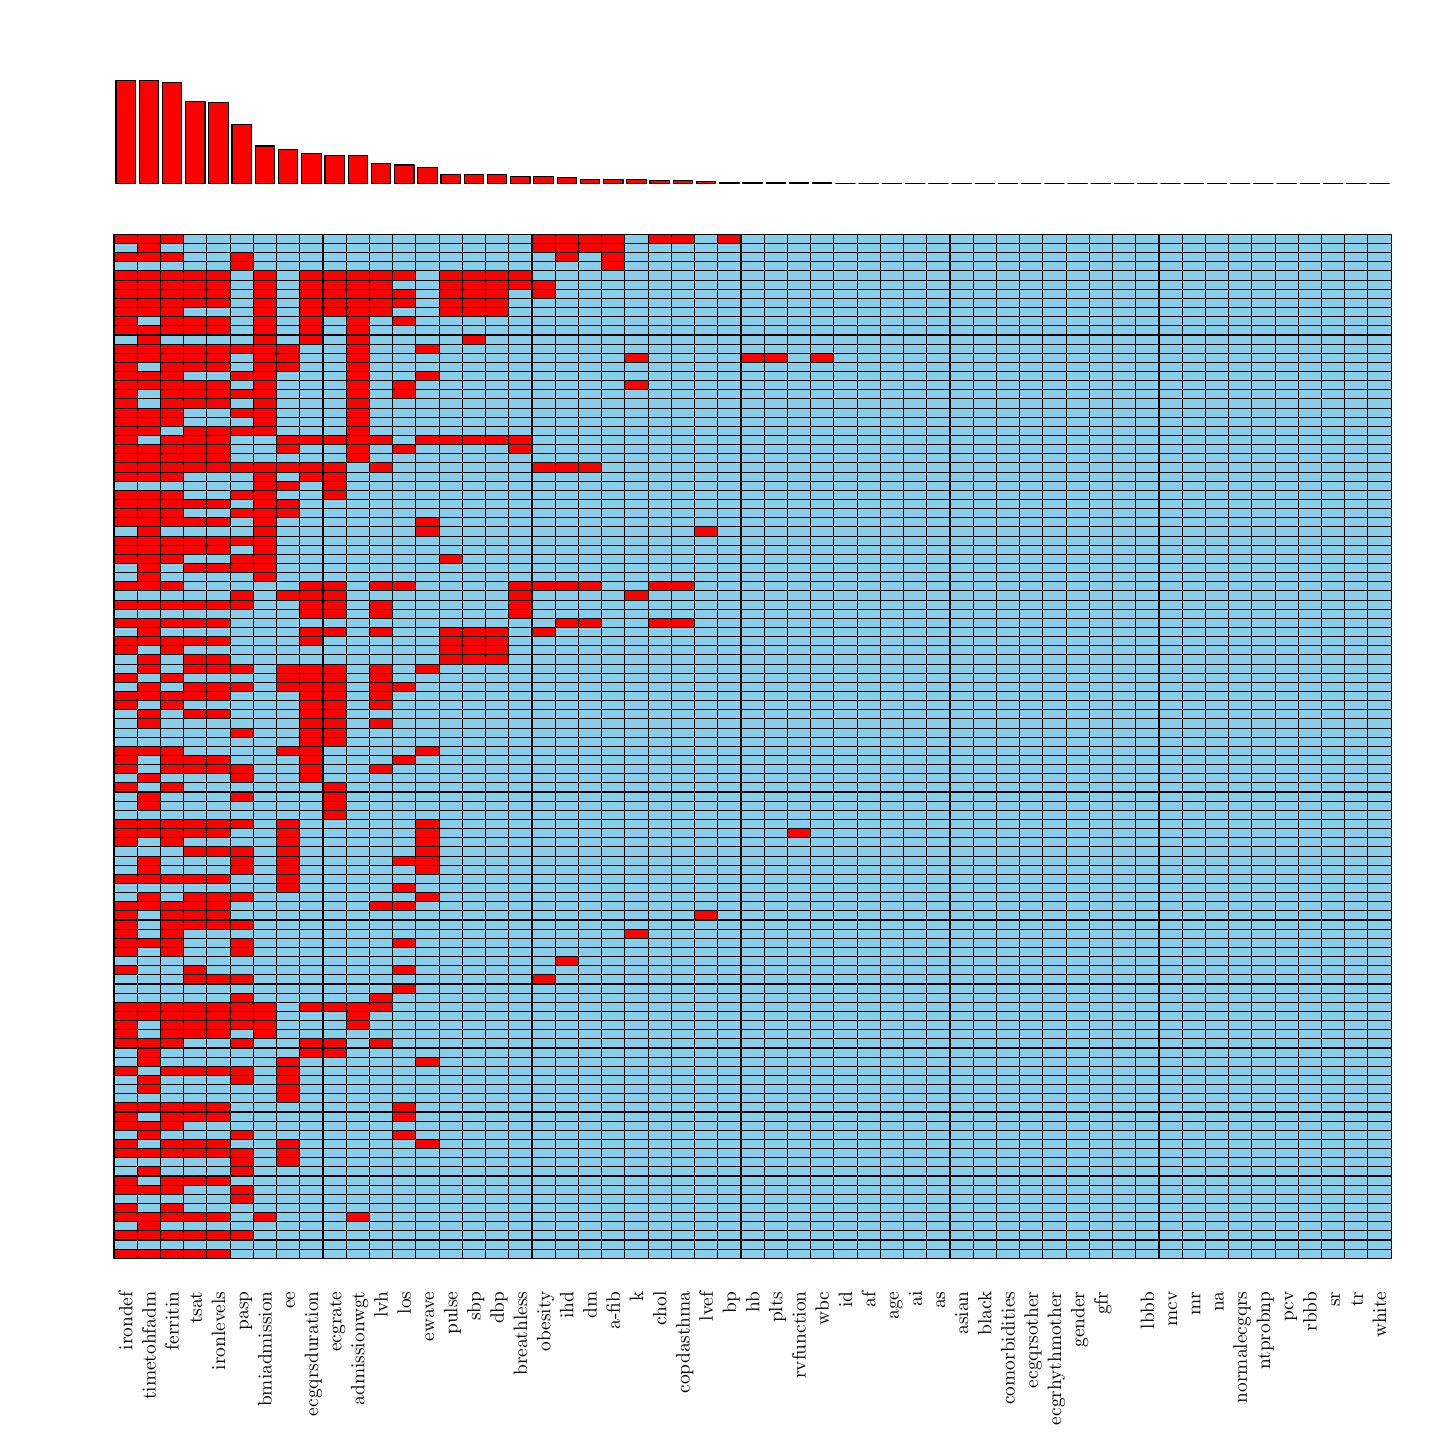
\begin{tikzpicture}[x=1pt,y=1pt]
\definecolor{fillColor}{RGB}{255,255,255}
\path[use as bounding box,fill=fillColor,fill opacity=0.00] (0,0) rectangle (505.89,505.89);
\begin{scope}
\path[clip] (  0.00,  0.00) rectangle (505.89,505.89);
\definecolor{drawColor}{RGB}{0,0,0}
\definecolor{fillColor}{RGB}{255,0,0}

\path[draw=drawColor,line width= 0.4pt,line join=round,line cap=round,fill=fillColor] ( 31.90,449.69) rectangle ( 38.89,486.69);

\path[draw=drawColor,line width= 0.4pt,line join=round,line cap=round,fill=fillColor] ( 40.29,449.69) rectangle ( 47.28,486.69);

\path[draw=drawColor,line width= 0.4pt,line join=round,line cap=round,fill=fillColor] ( 48.68,449.69) rectangle ( 55.67,486.09);

\path[draw=drawColor,line width= 0.4pt,line join=round,line cap=round,fill=fillColor] ( 57.07,449.69) rectangle ( 64.06,479.23);

\path[draw=drawColor,line width= 0.4pt,line join=round,line cap=round,fill=fillColor] ( 65.46,449.69) rectangle ( 72.45,478.93);

\path[draw=drawColor,line width= 0.4pt,line join=round,line cap=round,fill=fillColor] ( 73.85,449.69) rectangle ( 80.85,470.88);

\path[draw=drawColor,line width= 0.4pt,line join=round,line cap=round,fill=fillColor] ( 82.24,449.69) rectangle ( 89.24,463.12);

\path[draw=drawColor,line width= 0.4pt,line join=round,line cap=round,fill=fillColor] ( 90.63,449.69) rectangle ( 97.63,461.92);

\path[draw=drawColor,line width= 0.4pt,line join=round,line cap=round,fill=fillColor] ( 99.03,449.69) rectangle (106.02,460.43);

\path[draw=drawColor,line width= 0.4pt,line join=round,line cap=round,fill=fillColor] (107.42,449.69) rectangle (114.41,459.84);

\path[draw=drawColor,line width= 0.4pt,line join=round,line cap=round,fill=fillColor] (115.81,449.69) rectangle (122.80,459.54);

\path[draw=drawColor,line width= 0.4pt,line join=round,line cap=round,fill=fillColor] (124.20,449.69) rectangle (131.19,456.85);

\path[draw=drawColor,line width= 0.4pt,line join=round,line cap=round,fill=fillColor] (132.59,449.69) rectangle (139.58,456.26);

\path[draw=drawColor,line width= 0.4pt,line join=round,line cap=round,fill=fillColor] (140.98,449.69) rectangle (147.97,455.36);

\path[draw=drawColor,line width= 0.4pt,line join=round,line cap=round,fill=fillColor] (149.37,449.69) rectangle (156.36,452.97);

\path[draw=drawColor,line width= 0.4pt,line join=round,line cap=round,fill=fillColor] (157.76,449.69) rectangle (164.75,452.97);

\path[draw=drawColor,line width= 0.4pt,line join=round,line cap=round,fill=fillColor] (166.15,449.69) rectangle (173.14,452.67);

\path[draw=drawColor,line width= 0.4pt,line join=round,line cap=round,fill=fillColor] (174.54,449.69) rectangle (181.53,452.08);

\path[draw=drawColor,line width= 0.4pt,line join=round,line cap=round,fill=fillColor] (182.93,449.69) rectangle (189.92,452.08);

\path[draw=drawColor,line width= 0.4pt,line join=round,line cap=round,fill=fillColor] (191.32,449.69) rectangle (198.32,451.78);

\path[draw=drawColor,line width= 0.4pt,line join=round,line cap=round,fill=fillColor] (199.71,449.69) rectangle (206.71,451.18);

\path[draw=drawColor,line width= 0.4pt,line join=round,line cap=round,fill=fillColor] (208.10,449.69) rectangle (215.10,450.88);

\path[draw=drawColor,line width= 0.4pt,line join=round,line cap=round,fill=fillColor] (216.50,449.69) rectangle (223.49,450.88);

\path[draw=drawColor,line width= 0.4pt,line join=round,line cap=round,fill=fillColor] (224.89,449.69) rectangle (231.88,450.59);

\path[draw=drawColor,line width= 0.4pt,line join=round,line cap=round,fill=fillColor] (233.28,449.69) rectangle (240.27,450.59);

\path[draw=drawColor,line width= 0.4pt,line join=round,line cap=round,fill=fillColor] (241.67,449.69) rectangle (248.66,450.29);

\path[draw=drawColor,line width= 0.4pt,line join=round,line cap=round,fill=fillColor] (250.06,449.69) rectangle (257.05,449.99);

\path[draw=drawColor,line width= 0.4pt,line join=round,line cap=round,fill=fillColor] (258.45,449.69) rectangle (265.44,449.99);

\path[draw=drawColor,line width= 0.4pt,line join=round,line cap=round,fill=fillColor] (266.84,449.69) rectangle (273.83,449.99);

\path[draw=drawColor,line width= 0.4pt,line join=round,line cap=round,fill=fillColor] (275.23,449.69) rectangle (282.22,449.99);

\path[draw=drawColor,line width= 0.4pt,line join=round,line cap=round,fill=fillColor] (283.62,449.69) rectangle (290.61,449.99);

\path[draw=drawColor,line width= 0.4pt,line join=round,line cap=round,fill=fillColor] (292.01,449.69) rectangle (299.00,449.69);

\path[draw=drawColor,line width= 0.4pt,line join=round,line cap=round,fill=fillColor] (300.40,449.69) rectangle (307.39,449.69);

\path[draw=drawColor,line width= 0.4pt,line join=round,line cap=round,fill=fillColor] (308.79,449.69) rectangle (315.79,449.69);

\path[draw=drawColor,line width= 0.4pt,line join=round,line cap=round,fill=fillColor] (317.18,449.69) rectangle (324.18,449.69);

\path[draw=drawColor,line width= 0.4pt,line join=round,line cap=round,fill=fillColor] (325.57,449.69) rectangle (332.57,449.69);

\path[draw=drawColor,line width= 0.4pt,line join=round,line cap=round,fill=fillColor] (333.97,449.69) rectangle (340.96,449.69);

\path[draw=drawColor,line width= 0.4pt,line join=round,line cap=round,fill=fillColor] (342.36,449.69) rectangle (349.35,449.69);

\path[draw=drawColor,line width= 0.4pt,line join=round,line cap=round,fill=fillColor] (350.75,449.69) rectangle (357.74,449.69);

\path[draw=drawColor,line width= 0.4pt,line join=round,line cap=round,fill=fillColor] (359.14,449.69) rectangle (366.13,449.69);

\path[draw=drawColor,line width= 0.4pt,line join=round,line cap=round,fill=fillColor] (367.53,449.69) rectangle (374.52,449.69);

\path[draw=drawColor,line width= 0.4pt,line join=round,line cap=round,fill=fillColor] (375.92,449.69) rectangle (382.91,449.69);

\path[draw=drawColor,line width= 0.4pt,line join=round,line cap=round,fill=fillColor] (384.31,449.69) rectangle (391.30,449.69);

\path[draw=drawColor,line width= 0.4pt,line join=round,line cap=round,fill=fillColor] (392.70,449.69) rectangle (399.69,449.69);

\path[draw=drawColor,line width= 0.4pt,line join=round,line cap=round,fill=fillColor] (401.09,449.69) rectangle (408.08,449.69);

\path[draw=drawColor,line width= 0.4pt,line join=round,line cap=round,fill=fillColor] (409.48,449.69) rectangle (416.47,449.69);

\path[draw=drawColor,line width= 0.4pt,line join=round,line cap=round,fill=fillColor] (417.87,449.69) rectangle (424.86,449.69);

\path[draw=drawColor,line width= 0.4pt,line join=round,line cap=round,fill=fillColor] (426.26,449.69) rectangle (433.26,449.69);

\path[draw=drawColor,line width= 0.4pt,line join=round,line cap=round,fill=fillColor] (434.65,449.69) rectangle (441.65,449.69);

\path[draw=drawColor,line width= 0.4pt,line join=round,line cap=round,fill=fillColor] (443.04,449.69) rectangle (450.04,449.69);

\path[draw=drawColor,line width= 0.4pt,line join=round,line cap=round,fill=fillColor] (451.44,449.69) rectangle (458.43,449.69);

\path[draw=drawColor,line width= 0.4pt,line join=round,line cap=round,fill=fillColor] (459.83,449.69) rectangle (466.82,449.69);

\path[draw=drawColor,line width= 0.4pt,line join=round,line cap=round,fill=fillColor] (468.22,449.69) rectangle (475.21,449.69);

\path[draw=drawColor,line width= 0.4pt,line join=round,line cap=round,fill=fillColor] (476.61,449.69) rectangle (483.60,449.69);

\path[draw=drawColor,line width= 0.4pt,line join=round,line cap=round,fill=fillColor] (485.00,449.69) rectangle (491.99,449.69);
\end{scope}
\begin{scope}
\path[clip] (  0.00,  0.00) rectangle (505.89,505.89);
\definecolor{drawColor}{RGB}{0,0,0}
\definecolor{fillColor}{RGB}{255,0,0}

\path[draw=drawColor,line width= 0.4pt,line join=round,line cap=round,fill=fillColor] ( 31.20, 61.20) rectangle ( 39.59, 64.50);
\definecolor{fillColor}{RGB}{135,206,235}

\path[draw=drawColor,line width= 0.4pt,line join=round,line cap=round,fill=fillColor] ( 31.20, 64.50) rectangle ( 39.59, 67.81);
\definecolor{fillColor}{RGB}{255,0,0}

\path[draw=drawColor,line width= 0.4pt,line join=round,line cap=round,fill=fillColor] ( 31.20, 67.81) rectangle ( 39.59, 71.11);
\definecolor{fillColor}{RGB}{135,206,235}

\path[draw=drawColor,line width= 0.4pt,line join=round,line cap=round,fill=fillColor] ( 31.20, 71.11) rectangle ( 39.59, 74.41);
\definecolor{fillColor}{RGB}{255,0,0}

\path[draw=drawColor,line width= 0.4pt,line join=round,line cap=round,fill=fillColor] ( 31.20, 74.41) rectangle ( 39.59, 77.72);

\path[draw=drawColor,line width= 0.4pt,line join=round,line cap=round,fill=fillColor] ( 31.20, 77.72) rectangle ( 39.59, 81.02);
\definecolor{fillColor}{RGB}{135,206,235}

\path[draw=drawColor,line width= 0.4pt,line join=round,line cap=round,fill=fillColor] ( 31.20, 81.02) rectangle ( 39.59, 84.32);
\definecolor{fillColor}{RGB}{255,0,0}

\path[draw=drawColor,line width= 0.4pt,line join=round,line cap=round,fill=fillColor] ( 31.20, 84.32) rectangle ( 39.59, 87.63);

\path[draw=drawColor,line width= 0.4pt,line join=round,line cap=round,fill=fillColor] ( 31.20, 87.63) rectangle ( 39.59, 90.93);
\definecolor{fillColor}{RGB}{135,206,235}

\path[draw=drawColor,line width= 0.4pt,line join=round,line cap=round,fill=fillColor] ( 31.20, 90.93) rectangle ( 39.59, 94.23);

\path[draw=drawColor,line width= 0.4pt,line join=round,line cap=round,fill=fillColor] ( 31.20, 94.23) rectangle ( 39.59, 97.54);
\definecolor{fillColor}{RGB}{255,0,0}

\path[draw=drawColor,line width= 0.4pt,line join=round,line cap=round,fill=fillColor] ( 31.20, 97.54) rectangle ( 39.59,100.84);

\path[draw=drawColor,line width= 0.4pt,line join=round,line cap=round,fill=fillColor] ( 31.20,100.84) rectangle ( 39.59,104.15);
\definecolor{fillColor}{RGB}{135,206,235}

\path[draw=drawColor,line width= 0.4pt,line join=round,line cap=round,fill=fillColor] ( 31.20,104.15) rectangle ( 39.59,107.45);
\definecolor{fillColor}{RGB}{255,0,0}

\path[draw=drawColor,line width= 0.4pt,line join=round,line cap=round,fill=fillColor] ( 31.20,107.45) rectangle ( 39.59,110.75);

\path[draw=drawColor,line width= 0.4pt,line join=round,line cap=round,fill=fillColor] ( 31.20,110.75) rectangle ( 39.59,114.06);

\path[draw=drawColor,line width= 0.4pt,line join=round,line cap=round,fill=fillColor] ( 31.20,114.06) rectangle ( 39.59,117.36);
\definecolor{fillColor}{RGB}{135,206,235}

\path[draw=drawColor,line width= 0.4pt,line join=round,line cap=round,fill=fillColor] ( 31.20,117.36) rectangle ( 39.59,120.66);

\path[draw=drawColor,line width= 0.4pt,line join=round,line cap=round,fill=fillColor] ( 31.20,120.66) rectangle ( 39.59,123.97);

\path[draw=drawColor,line width= 0.4pt,line join=round,line cap=round,fill=fillColor] ( 31.20,123.97) rectangle ( 39.59,127.27);
\definecolor{fillColor}{RGB}{255,0,0}

\path[draw=drawColor,line width= 0.4pt,line join=round,line cap=round,fill=fillColor] ( 31.20,127.27) rectangle ( 39.59,130.57);
\definecolor{fillColor}{RGB}{135,206,235}

\path[draw=drawColor,line width= 0.4pt,line join=round,line cap=round,fill=fillColor] ( 31.20,130.57) rectangle ( 39.59,133.88);

\path[draw=drawColor,line width= 0.4pt,line join=round,line cap=round,fill=fillColor] ( 31.20,133.88) rectangle ( 39.59,137.18);
\definecolor{fillColor}{RGB}{255,0,0}

\path[draw=drawColor,line width= 0.4pt,line join=round,line cap=round,fill=fillColor] ( 31.20,137.18) rectangle ( 39.59,140.48);

\path[draw=drawColor,line width= 0.4pt,line join=round,line cap=round,fill=fillColor] ( 31.20,140.48) rectangle ( 39.59,143.79);

\path[draw=drawColor,line width= 0.4pt,line join=round,line cap=round,fill=fillColor] ( 31.20,143.79) rectangle ( 39.59,147.09);

\path[draw=drawColor,line width= 0.4pt,line join=round,line cap=round,fill=fillColor] ( 31.20,147.09) rectangle ( 39.59,150.39);

\path[draw=drawColor,line width= 0.4pt,line join=round,line cap=round,fill=fillColor] ( 31.20,150.39) rectangle ( 39.59,153.70);
\definecolor{fillColor}{RGB}{135,206,235}

\path[draw=drawColor,line width= 0.4pt,line join=round,line cap=round,fill=fillColor] ( 31.20,153.70) rectangle ( 39.59,157.00);

\path[draw=drawColor,line width= 0.4pt,line join=round,line cap=round,fill=fillColor] ( 31.20,157.00) rectangle ( 39.59,160.30);

\path[draw=drawColor,line width= 0.4pt,line join=round,line cap=round,fill=fillColor] ( 31.20,160.30) rectangle ( 39.59,163.61);
\definecolor{fillColor}{RGB}{255,0,0}

\path[draw=drawColor,line width= 0.4pt,line join=round,line cap=round,fill=fillColor] ( 31.20,163.61) rectangle ( 39.59,166.91);
\definecolor{fillColor}{RGB}{135,206,235}

\path[draw=drawColor,line width= 0.4pt,line join=round,line cap=round,fill=fillColor] ( 31.20,166.91) rectangle ( 39.59,170.22);
\definecolor{fillColor}{RGB}{255,0,0}

\path[draw=drawColor,line width= 0.4pt,line join=round,line cap=round,fill=fillColor] ( 31.20,170.22) rectangle ( 39.59,173.52);

\path[draw=drawColor,line width= 0.4pt,line join=round,line cap=round,fill=fillColor] ( 31.20,173.52) rectangle ( 39.59,176.82);

\path[draw=drawColor,line width= 0.4pt,line join=round,line cap=round,fill=fillColor] ( 31.20,176.82) rectangle ( 39.59,180.13);

\path[draw=drawColor,line width= 0.4pt,line join=round,line cap=round,fill=fillColor] ( 31.20,180.13) rectangle ( 39.59,183.43);

\path[draw=drawColor,line width= 0.4pt,line join=round,line cap=round,fill=fillColor] ( 31.20,183.43) rectangle ( 39.59,186.73);

\path[draw=drawColor,line width= 0.4pt,line join=round,line cap=round,fill=fillColor] ( 31.20,186.73) rectangle ( 39.59,190.04);
\definecolor{fillColor}{RGB}{135,206,235}

\path[draw=drawColor,line width= 0.4pt,line join=round,line cap=round,fill=fillColor] ( 31.20,190.04) rectangle ( 39.59,193.34);

\path[draw=drawColor,line width= 0.4pt,line join=round,line cap=round,fill=fillColor] ( 31.20,193.34) rectangle ( 39.59,196.64);
\definecolor{fillColor}{RGB}{255,0,0}

\path[draw=drawColor,line width= 0.4pt,line join=round,line cap=round,fill=fillColor] ( 31.20,196.64) rectangle ( 39.59,199.95);
\definecolor{fillColor}{RGB}{135,206,235}

\path[draw=drawColor,line width= 0.4pt,line join=round,line cap=round,fill=fillColor] ( 31.20,199.95) rectangle ( 39.59,203.25);

\path[draw=drawColor,line width= 0.4pt,line join=round,line cap=round,fill=fillColor] ( 31.20,203.25) rectangle ( 39.59,206.55);

\path[draw=drawColor,line width= 0.4pt,line join=round,line cap=round,fill=fillColor] ( 31.20,206.55) rectangle ( 39.59,209.86);
\definecolor{fillColor}{RGB}{255,0,0}

\path[draw=drawColor,line width= 0.4pt,line join=round,line cap=round,fill=fillColor] ( 31.20,209.86) rectangle ( 39.59,213.16);

\path[draw=drawColor,line width= 0.4pt,line join=round,line cap=round,fill=fillColor] ( 31.20,213.16) rectangle ( 39.59,216.46);

\path[draw=drawColor,line width= 0.4pt,line join=round,line cap=round,fill=fillColor] ( 31.20,216.46) rectangle ( 39.59,219.77);
\definecolor{fillColor}{RGB}{135,206,235}

\path[draw=drawColor,line width= 0.4pt,line join=round,line cap=round,fill=fillColor] ( 31.20,219.77) rectangle ( 39.59,223.07);

\path[draw=drawColor,line width= 0.4pt,line join=round,line cap=round,fill=fillColor] ( 31.20,223.07) rectangle ( 39.59,226.37);

\path[draw=drawColor,line width= 0.4pt,line join=round,line cap=round,fill=fillColor] ( 31.20,226.37) rectangle ( 39.59,229.68);
\definecolor{fillColor}{RGB}{255,0,0}

\path[draw=drawColor,line width= 0.4pt,line join=round,line cap=round,fill=fillColor] ( 31.20,229.68) rectangle ( 39.59,232.98);
\definecolor{fillColor}{RGB}{135,206,235}

\path[draw=drawColor,line width= 0.4pt,line join=round,line cap=round,fill=fillColor] ( 31.20,232.98) rectangle ( 39.59,236.29);
\definecolor{fillColor}{RGB}{255,0,0}

\path[draw=drawColor,line width= 0.4pt,line join=round,line cap=round,fill=fillColor] ( 31.20,236.29) rectangle ( 39.59,239.59);

\path[draw=drawColor,line width= 0.4pt,line join=round,line cap=round,fill=fillColor] ( 31.20,239.59) rectangle ( 39.59,242.89);

\path[draw=drawColor,line width= 0.4pt,line join=round,line cap=round,fill=fillColor] ( 31.20,242.89) rectangle ( 39.59,246.20);
\definecolor{fillColor}{RGB}{135,206,235}

\path[draw=drawColor,line width= 0.4pt,line join=round,line cap=round,fill=fillColor] ( 31.20,246.20) rectangle ( 39.59,249.50);

\path[draw=drawColor,line width= 0.4pt,line join=round,line cap=round,fill=fillColor] ( 31.20,249.50) rectangle ( 39.59,252.80);

\path[draw=drawColor,line width= 0.4pt,line join=round,line cap=round,fill=fillColor] ( 31.20,252.80) rectangle ( 39.59,256.11);

\path[draw=drawColor,line width= 0.4pt,line join=round,line cap=round,fill=fillColor] ( 31.20,256.11) rectangle ( 39.59,259.41);
\definecolor{fillColor}{RGB}{255,0,0}

\path[draw=drawColor,line width= 0.4pt,line join=round,line cap=round,fill=fillColor] ( 31.20,259.41) rectangle ( 39.59,262.71);

\path[draw=drawColor,line width= 0.4pt,line join=round,line cap=round,fill=fillColor] ( 31.20,262.71) rectangle ( 39.59,266.02);
\definecolor{fillColor}{RGB}{135,206,235}

\path[draw=drawColor,line width= 0.4pt,line join=round,line cap=round,fill=fillColor] ( 31.20,266.02) rectangle ( 39.59,269.32);
\definecolor{fillColor}{RGB}{255,0,0}

\path[draw=drawColor,line width= 0.4pt,line join=round,line cap=round,fill=fillColor] ( 31.20,269.32) rectangle ( 39.59,272.62);
\definecolor{fillColor}{RGB}{135,206,235}

\path[draw=drawColor,line width= 0.4pt,line join=round,line cap=round,fill=fillColor] ( 31.20,272.62) rectangle ( 39.59,275.93);

\path[draw=drawColor,line width= 0.4pt,line join=round,line cap=round,fill=fillColor] ( 31.20,275.93) rectangle ( 39.59,279.23);
\definecolor{fillColor}{RGB}{255,0,0}

\path[draw=drawColor,line width= 0.4pt,line join=round,line cap=round,fill=fillColor] ( 31.20,279.23) rectangle ( 39.59,282.53);

\path[draw=drawColor,line width= 0.4pt,line join=round,line cap=round,fill=fillColor] ( 31.20,282.53) rectangle ( 39.59,285.84);
\definecolor{fillColor}{RGB}{135,206,235}

\path[draw=drawColor,line width= 0.4pt,line join=round,line cap=round,fill=fillColor] ( 31.20,285.84) rectangle ( 39.59,289.14);
\definecolor{fillColor}{RGB}{255,0,0}

\path[draw=drawColor,line width= 0.4pt,line join=round,line cap=round,fill=fillColor] ( 31.20,289.14) rectangle ( 39.59,292.44);
\definecolor{fillColor}{RGB}{135,206,235}

\path[draw=drawColor,line width= 0.4pt,line join=round,line cap=round,fill=fillColor] ( 31.20,292.44) rectangle ( 39.59,295.75);
\definecolor{fillColor}{RGB}{255,0,0}

\path[draw=drawColor,line width= 0.4pt,line join=round,line cap=round,fill=fillColor] ( 31.20,295.75) rectangle ( 39.59,299.05);
\definecolor{fillColor}{RGB}{135,206,235}

\path[draw=drawColor,line width= 0.4pt,line join=round,line cap=round,fill=fillColor] ( 31.20,299.05) rectangle ( 39.59,302.36);
\definecolor{fillColor}{RGB}{255,0,0}

\path[draw=drawColor,line width= 0.4pt,line join=round,line cap=round,fill=fillColor] ( 31.20,302.36) rectangle ( 39.59,305.66);
\definecolor{fillColor}{RGB}{135,206,235}

\path[draw=drawColor,line width= 0.4pt,line join=round,line cap=round,fill=fillColor] ( 31.20,305.66) rectangle ( 39.59,308.96);

\path[draw=drawColor,line width= 0.4pt,line join=round,line cap=round,fill=fillColor] ( 31.20,308.96) rectangle ( 39.59,312.27);
\definecolor{fillColor}{RGB}{255,0,0}

\path[draw=drawColor,line width= 0.4pt,line join=round,line cap=round,fill=fillColor] ( 31.20,312.27) rectangle ( 39.59,315.57);

\path[draw=drawColor,line width= 0.4pt,line join=round,line cap=round,fill=fillColor] ( 31.20,315.57) rectangle ( 39.59,318.87);

\path[draw=drawColor,line width= 0.4pt,line join=round,line cap=round,fill=fillColor] ( 31.20,318.87) rectangle ( 39.59,322.18);
\definecolor{fillColor}{RGB}{135,206,235}

\path[draw=drawColor,line width= 0.4pt,line join=round,line cap=round,fill=fillColor] ( 31.20,322.18) rectangle ( 39.59,325.48);
\definecolor{fillColor}{RGB}{255,0,0}

\path[draw=drawColor,line width= 0.4pt,line join=round,line cap=round,fill=fillColor] ( 31.20,325.48) rectangle ( 39.59,328.78);

\path[draw=drawColor,line width= 0.4pt,line join=round,line cap=round,fill=fillColor] ( 31.20,328.78) rectangle ( 39.59,332.09);

\path[draw=drawColor,line width= 0.4pt,line join=round,line cap=round,fill=fillColor] ( 31.20,332.09) rectangle ( 39.59,335.39);

\path[draw=drawColor,line width= 0.4pt,line join=round,line cap=round,fill=fillColor] ( 31.20,335.39) rectangle ( 39.59,338.69);
\definecolor{fillColor}{RGB}{135,206,235}

\path[draw=drawColor,line width= 0.4pt,line join=round,line cap=round,fill=fillColor] ( 31.20,338.69) rectangle ( 39.59,342.00);
\definecolor{fillColor}{RGB}{255,0,0}

\path[draw=drawColor,line width= 0.4pt,line join=round,line cap=round,fill=fillColor] ( 31.20,342.00) rectangle ( 39.59,345.30);

\path[draw=drawColor,line width= 0.4pt,line join=round,line cap=round,fill=fillColor] ( 31.20,345.30) rectangle ( 39.59,348.60);

\path[draw=drawColor,line width= 0.4pt,line join=round,line cap=round,fill=fillColor] ( 31.20,348.60) rectangle ( 39.59,351.91);

\path[draw=drawColor,line width= 0.4pt,line join=round,line cap=round,fill=fillColor] ( 31.20,351.91) rectangle ( 39.59,355.21);

\path[draw=drawColor,line width= 0.4pt,line join=round,line cap=round,fill=fillColor] ( 31.20,355.21) rectangle ( 39.59,358.51);

\path[draw=drawColor,line width= 0.4pt,line join=round,line cap=round,fill=fillColor] ( 31.20,358.51) rectangle ( 39.59,361.82);

\path[draw=drawColor,line width= 0.4pt,line join=round,line cap=round,fill=fillColor] ( 31.20,361.82) rectangle ( 39.59,365.12);

\path[draw=drawColor,line width= 0.4pt,line join=round,line cap=round,fill=fillColor] ( 31.20,365.12) rectangle ( 39.59,368.42);

\path[draw=drawColor,line width= 0.4pt,line join=round,line cap=round,fill=fillColor] ( 31.20,368.42) rectangle ( 39.59,371.73);

\path[draw=drawColor,line width= 0.4pt,line join=round,line cap=round,fill=fillColor] ( 31.20,371.73) rectangle ( 39.59,375.03);

\path[draw=drawColor,line width= 0.4pt,line join=round,line cap=round,fill=fillColor] ( 31.20,375.03) rectangle ( 39.59,378.34);

\path[draw=drawColor,line width= 0.4pt,line join=round,line cap=round,fill=fillColor] ( 31.20,378.34) rectangle ( 39.59,381.64);

\path[draw=drawColor,line width= 0.4pt,line join=round,line cap=round,fill=fillColor] ( 31.20,381.64) rectangle ( 39.59,384.94);

\path[draw=drawColor,line width= 0.4pt,line join=round,line cap=round,fill=fillColor] ( 31.20,384.94) rectangle ( 39.59,388.25);

\path[draw=drawColor,line width= 0.4pt,line join=round,line cap=round,fill=fillColor] ( 31.20,388.25) rectangle ( 39.59,391.55);
\definecolor{fillColor}{RGB}{135,206,235}

\path[draw=drawColor,line width= 0.4pt,line join=round,line cap=round,fill=fillColor] ( 31.20,391.55) rectangle ( 39.59,394.85);
\definecolor{fillColor}{RGB}{255,0,0}

\path[draw=drawColor,line width= 0.4pt,line join=round,line cap=round,fill=fillColor] ( 31.20,394.85) rectangle ( 39.59,398.16);

\path[draw=drawColor,line width= 0.4pt,line join=round,line cap=round,fill=fillColor] ( 31.20,398.16) rectangle ( 39.59,401.46);

\path[draw=drawColor,line width= 0.4pt,line join=round,line cap=round,fill=fillColor] ( 31.20,401.46) rectangle ( 39.59,404.76);

\path[draw=drawColor,line width= 0.4pt,line join=round,line cap=round,fill=fillColor] ( 31.20,404.76) rectangle ( 39.59,408.07);

\path[draw=drawColor,line width= 0.4pt,line join=round,line cap=round,fill=fillColor] ( 31.20,408.07) rectangle ( 39.59,411.37);

\path[draw=drawColor,line width= 0.4pt,line join=round,line cap=round,fill=fillColor] ( 31.20,411.37) rectangle ( 39.59,414.67);

\path[draw=drawColor,line width= 0.4pt,line join=round,line cap=round,fill=fillColor] ( 31.20,414.67) rectangle ( 39.59,417.98);
\definecolor{fillColor}{RGB}{135,206,235}

\path[draw=drawColor,line width= 0.4pt,line join=round,line cap=round,fill=fillColor] ( 31.20,417.98) rectangle ( 39.59,421.28);
\definecolor{fillColor}{RGB}{255,0,0}

\path[draw=drawColor,line width= 0.4pt,line join=round,line cap=round,fill=fillColor] ( 31.20,421.28) rectangle ( 39.59,424.58);
\definecolor{fillColor}{RGB}{135,206,235}

\path[draw=drawColor,line width= 0.4pt,line join=round,line cap=round,fill=fillColor] ( 31.20,424.58) rectangle ( 39.59,427.89);
\definecolor{fillColor}{RGB}{255,0,0}

\path[draw=drawColor,line width= 0.4pt,line join=round,line cap=round,fill=fillColor] ( 31.20,427.89) rectangle ( 39.59,431.19);

\path[draw=drawColor,line width= 0.4pt,line join=round,line cap=round,fill=fillColor] ( 39.59, 61.20) rectangle ( 47.98, 64.50);
\definecolor{fillColor}{RGB}{135,206,235}

\path[draw=drawColor,line width= 0.4pt,line join=round,line cap=round,fill=fillColor] ( 39.59, 64.50) rectangle ( 47.98, 67.81);
\definecolor{fillColor}{RGB}{255,0,0}

\path[draw=drawColor,line width= 0.4pt,line join=round,line cap=round,fill=fillColor] ( 39.59, 67.81) rectangle ( 47.98, 71.11);

\path[draw=drawColor,line width= 0.4pt,line join=round,line cap=round,fill=fillColor] ( 39.59, 71.11) rectangle ( 47.98, 74.41);

\path[draw=drawColor,line width= 0.4pt,line join=round,line cap=round,fill=fillColor] ( 39.59, 74.41) rectangle ( 47.98, 77.72);
\definecolor{fillColor}{RGB}{135,206,235}

\path[draw=drawColor,line width= 0.4pt,line join=round,line cap=round,fill=fillColor] ( 39.59, 77.72) rectangle ( 47.98, 81.02);

\path[draw=drawColor,line width= 0.4pt,line join=round,line cap=round,fill=fillColor] ( 39.59, 81.02) rectangle ( 47.98, 84.32);
\definecolor{fillColor}{RGB}{255,0,0}

\path[draw=drawColor,line width= 0.4pt,line join=round,line cap=round,fill=fillColor] ( 39.59, 84.32) rectangle ( 47.98, 87.63);
\definecolor{fillColor}{RGB}{135,206,235}

\path[draw=drawColor,line width= 0.4pt,line join=round,line cap=round,fill=fillColor] ( 39.59, 87.63) rectangle ( 47.98, 90.93);
\definecolor{fillColor}{RGB}{255,0,0}

\path[draw=drawColor,line width= 0.4pt,line join=round,line cap=round,fill=fillColor] ( 39.59, 90.93) rectangle ( 47.98, 94.23);
\definecolor{fillColor}{RGB}{135,206,235}

\path[draw=drawColor,line width= 0.4pt,line join=round,line cap=round,fill=fillColor] ( 39.59, 94.23) rectangle ( 47.98, 97.54);
\definecolor{fillColor}{RGB}{255,0,0}

\path[draw=drawColor,line width= 0.4pt,line join=round,line cap=round,fill=fillColor] ( 39.59, 97.54) rectangle ( 47.98,100.84);
\definecolor{fillColor}{RGB}{135,206,235}

\path[draw=drawColor,line width= 0.4pt,line join=round,line cap=round,fill=fillColor] ( 39.59,100.84) rectangle ( 47.98,104.15);
\definecolor{fillColor}{RGB}{255,0,0}

\path[draw=drawColor,line width= 0.4pt,line join=round,line cap=round,fill=fillColor] ( 39.59,104.15) rectangle ( 47.98,107.45);

\path[draw=drawColor,line width= 0.4pt,line join=round,line cap=round,fill=fillColor] ( 39.59,107.45) rectangle ( 47.98,110.75);
\definecolor{fillColor}{RGB}{135,206,235}

\path[draw=drawColor,line width= 0.4pt,line join=round,line cap=round,fill=fillColor] ( 39.59,110.75) rectangle ( 47.98,114.06);
\definecolor{fillColor}{RGB}{255,0,0}

\path[draw=drawColor,line width= 0.4pt,line join=round,line cap=round,fill=fillColor] ( 39.59,114.06) rectangle ( 47.98,117.36);
\definecolor{fillColor}{RGB}{135,206,235}

\path[draw=drawColor,line width= 0.4pt,line join=round,line cap=round,fill=fillColor] ( 39.59,117.36) rectangle ( 47.98,120.66);
\definecolor{fillColor}{RGB}{255,0,0}

\path[draw=drawColor,line width= 0.4pt,line join=round,line cap=round,fill=fillColor] ( 39.59,120.66) rectangle ( 47.98,123.97);

\path[draw=drawColor,line width= 0.4pt,line join=round,line cap=round,fill=fillColor] ( 39.59,123.97) rectangle ( 47.98,127.27);
\definecolor{fillColor}{RGB}{135,206,235}

\path[draw=drawColor,line width= 0.4pt,line join=round,line cap=round,fill=fillColor] ( 39.59,127.27) rectangle ( 47.98,130.57);
\definecolor{fillColor}{RGB}{255,0,0}

\path[draw=drawColor,line width= 0.4pt,line join=round,line cap=round,fill=fillColor] ( 39.59,130.57) rectangle ( 47.98,133.88);

\path[draw=drawColor,line width= 0.4pt,line join=round,line cap=round,fill=fillColor] ( 39.59,133.88) rectangle ( 47.98,137.18);

\path[draw=drawColor,line width= 0.4pt,line join=round,line cap=round,fill=fillColor] ( 39.59,137.18) rectangle ( 47.98,140.48);
\definecolor{fillColor}{RGB}{135,206,235}

\path[draw=drawColor,line width= 0.4pt,line join=round,line cap=round,fill=fillColor] ( 39.59,140.48) rectangle ( 47.98,143.79);

\path[draw=drawColor,line width= 0.4pt,line join=round,line cap=round,fill=fillColor] ( 39.59,143.79) rectangle ( 47.98,147.09);
\definecolor{fillColor}{RGB}{255,0,0}

\path[draw=drawColor,line width= 0.4pt,line join=round,line cap=round,fill=fillColor] ( 39.59,147.09) rectangle ( 47.98,150.39);

\path[draw=drawColor,line width= 0.4pt,line join=round,line cap=round,fill=fillColor] ( 39.59,150.39) rectangle ( 47.98,153.70);
\definecolor{fillColor}{RGB}{135,206,235}

\path[draw=drawColor,line width= 0.4pt,line join=round,line cap=round,fill=fillColor] ( 39.59,153.70) rectangle ( 47.98,157.00);

\path[draw=drawColor,line width= 0.4pt,line join=round,line cap=round,fill=fillColor] ( 39.59,157.00) rectangle ( 47.98,160.30);

\path[draw=drawColor,line width= 0.4pt,line join=round,line cap=round,fill=fillColor] ( 39.59,160.30) rectangle ( 47.98,163.61);

\path[draw=drawColor,line width= 0.4pt,line join=round,line cap=round,fill=fillColor] ( 39.59,163.61) rectangle ( 47.98,166.91);

\path[draw=drawColor,line width= 0.4pt,line join=round,line cap=round,fill=fillColor] ( 39.59,166.91) rectangle ( 47.98,170.22);

\path[draw=drawColor,line width= 0.4pt,line join=round,line cap=round,fill=fillColor] ( 39.59,170.22) rectangle ( 47.98,173.52);
\definecolor{fillColor}{RGB}{255,0,0}

\path[draw=drawColor,line width= 0.4pt,line join=round,line cap=round,fill=fillColor] ( 39.59,173.52) rectangle ( 47.98,176.82);
\definecolor{fillColor}{RGB}{135,206,235}

\path[draw=drawColor,line width= 0.4pt,line join=round,line cap=round,fill=fillColor] ( 39.59,176.82) rectangle ( 47.98,180.13);

\path[draw=drawColor,line width= 0.4pt,line join=round,line cap=round,fill=fillColor] ( 39.59,180.13) rectangle ( 47.98,183.43);

\path[draw=drawColor,line width= 0.4pt,line join=round,line cap=round,fill=fillColor] ( 39.59,183.43) rectangle ( 47.98,186.73);
\definecolor{fillColor}{RGB}{255,0,0}

\path[draw=drawColor,line width= 0.4pt,line join=round,line cap=round,fill=fillColor] ( 39.59,186.73) rectangle ( 47.98,190.04);

\path[draw=drawColor,line width= 0.4pt,line join=round,line cap=round,fill=fillColor] ( 39.59,190.04) rectangle ( 47.98,193.34);
\definecolor{fillColor}{RGB}{135,206,235}

\path[draw=drawColor,line width= 0.4pt,line join=round,line cap=round,fill=fillColor] ( 39.59,193.34) rectangle ( 47.98,196.64);
\definecolor{fillColor}{RGB}{255,0,0}

\path[draw=drawColor,line width= 0.4pt,line join=round,line cap=round,fill=fillColor] ( 39.59,196.64) rectangle ( 47.98,199.95);

\path[draw=drawColor,line width= 0.4pt,line join=round,line cap=round,fill=fillColor] ( 39.59,199.95) rectangle ( 47.98,203.25);

\path[draw=drawColor,line width= 0.4pt,line join=round,line cap=round,fill=fillColor] ( 39.59,203.25) rectangle ( 47.98,206.55);
\definecolor{fillColor}{RGB}{135,206,235}

\path[draw=drawColor,line width= 0.4pt,line join=round,line cap=round,fill=fillColor] ( 39.59,206.55) rectangle ( 47.98,209.86);

\path[draw=drawColor,line width= 0.4pt,line join=round,line cap=round,fill=fillColor] ( 39.59,209.86) rectangle ( 47.98,213.16);
\definecolor{fillColor}{RGB}{255,0,0}

\path[draw=drawColor,line width= 0.4pt,line join=round,line cap=round,fill=fillColor] ( 39.59,213.16) rectangle ( 47.98,216.46);

\path[draw=drawColor,line width= 0.4pt,line join=round,line cap=round,fill=fillColor] ( 39.59,216.46) rectangle ( 47.98,219.77);
\definecolor{fillColor}{RGB}{135,206,235}

\path[draw=drawColor,line width= 0.4pt,line join=round,line cap=round,fill=fillColor] ( 39.59,219.77) rectangle ( 47.98,223.07);
\definecolor{fillColor}{RGB}{255,0,0}

\path[draw=drawColor,line width= 0.4pt,line join=round,line cap=round,fill=fillColor] ( 39.59,223.07) rectangle ( 47.98,226.37);

\path[draw=drawColor,line width= 0.4pt,line join=round,line cap=round,fill=fillColor] ( 39.59,226.37) rectangle ( 47.98,229.68);
\definecolor{fillColor}{RGB}{135,206,235}

\path[draw=drawColor,line width= 0.4pt,line join=round,line cap=round,fill=fillColor] ( 39.59,229.68) rectangle ( 47.98,232.98);
\definecolor{fillColor}{RGB}{255,0,0}

\path[draw=drawColor,line width= 0.4pt,line join=round,line cap=round,fill=fillColor] ( 39.59,232.98) rectangle ( 47.98,236.29);
\definecolor{fillColor}{RGB}{135,206,235}

\path[draw=drawColor,line width= 0.4pt,line join=round,line cap=round,fill=fillColor] ( 39.59,236.29) rectangle ( 47.98,239.59);

\path[draw=drawColor,line width= 0.4pt,line join=round,line cap=round,fill=fillColor] ( 39.59,239.59) rectangle ( 47.98,242.89);
\definecolor{fillColor}{RGB}{255,0,0}

\path[draw=drawColor,line width= 0.4pt,line join=round,line cap=round,fill=fillColor] ( 39.59,242.89) rectangle ( 47.98,246.20);
\definecolor{fillColor}{RGB}{135,206,235}

\path[draw=drawColor,line width= 0.4pt,line join=round,line cap=round,fill=fillColor] ( 39.59,246.20) rectangle ( 47.98,249.50);

\path[draw=drawColor,line width= 0.4pt,line join=round,line cap=round,fill=fillColor] ( 39.59,249.50) rectangle ( 47.98,252.80);
\definecolor{fillColor}{RGB}{255,0,0}

\path[draw=drawColor,line width= 0.4pt,line join=round,line cap=round,fill=fillColor] ( 39.59,252.80) rectangle ( 47.98,256.11);

\path[draw=drawColor,line width= 0.4pt,line join=round,line cap=round,fill=fillColor] ( 39.59,256.11) rectangle ( 47.98,259.41);
\definecolor{fillColor}{RGB}{135,206,235}

\path[draw=drawColor,line width= 0.4pt,line join=round,line cap=round,fill=fillColor] ( 39.59,259.41) rectangle ( 47.98,262.71);
\definecolor{fillColor}{RGB}{255,0,0}

\path[draw=drawColor,line width= 0.4pt,line join=round,line cap=round,fill=fillColor] ( 39.59,262.71) rectangle ( 47.98,266.02);

\path[draw=drawColor,line width= 0.4pt,line join=round,line cap=round,fill=fillColor] ( 39.59,266.02) rectangle ( 47.98,269.32);
\definecolor{fillColor}{RGB}{135,206,235}

\path[draw=drawColor,line width= 0.4pt,line join=round,line cap=round,fill=fillColor] ( 39.59,269.32) rectangle ( 47.98,272.62);
\definecolor{fillColor}{RGB}{255,0,0}

\path[draw=drawColor,line width= 0.4pt,line join=round,line cap=round,fill=fillColor] ( 39.59,272.62) rectangle ( 47.98,275.93);

\path[draw=drawColor,line width= 0.4pt,line join=round,line cap=round,fill=fillColor] ( 39.59,275.93) rectangle ( 47.98,279.23);
\definecolor{fillColor}{RGB}{135,206,235}

\path[draw=drawColor,line width= 0.4pt,line join=round,line cap=round,fill=fillColor] ( 39.59,279.23) rectangle ( 47.98,282.53);
\definecolor{fillColor}{RGB}{255,0,0}

\path[draw=drawColor,line width= 0.4pt,line join=round,line cap=round,fill=fillColor] ( 39.59,282.53) rectangle ( 47.98,285.84);

\path[draw=drawColor,line width= 0.4pt,line join=round,line cap=round,fill=fillColor] ( 39.59,285.84) rectangle ( 47.98,289.14);

\path[draw=drawColor,line width= 0.4pt,line join=round,line cap=round,fill=fillColor] ( 39.59,289.14) rectangle ( 47.98,292.44);
\definecolor{fillColor}{RGB}{135,206,235}

\path[draw=drawColor,line width= 0.4pt,line join=round,line cap=round,fill=fillColor] ( 39.59,292.44) rectangle ( 47.98,295.75);
\definecolor{fillColor}{RGB}{255,0,0}

\path[draw=drawColor,line width= 0.4pt,line join=round,line cap=round,fill=fillColor] ( 39.59,295.75) rectangle ( 47.98,299.05);
\definecolor{fillColor}{RGB}{135,206,235}

\path[draw=drawColor,line width= 0.4pt,line join=round,line cap=round,fill=fillColor] ( 39.59,299.05) rectangle ( 47.98,302.36);
\definecolor{fillColor}{RGB}{255,0,0}

\path[draw=drawColor,line width= 0.4pt,line join=round,line cap=round,fill=fillColor] ( 39.59,302.36) rectangle ( 47.98,305.66);

\path[draw=drawColor,line width= 0.4pt,line join=round,line cap=round,fill=fillColor] ( 39.59,305.66) rectangle ( 47.98,308.96);

\path[draw=drawColor,line width= 0.4pt,line join=round,line cap=round,fill=fillColor] ( 39.59,308.96) rectangle ( 47.98,312.27);

\path[draw=drawColor,line width= 0.4pt,line join=round,line cap=round,fill=fillColor] ( 39.59,312.27) rectangle ( 47.98,315.57);

\path[draw=drawColor,line width= 0.4pt,line join=round,line cap=round,fill=fillColor] ( 39.59,315.57) rectangle ( 47.98,318.87);

\path[draw=drawColor,line width= 0.4pt,line join=round,line cap=round,fill=fillColor] ( 39.59,318.87) rectangle ( 47.98,322.18);

\path[draw=drawColor,line width= 0.4pt,line join=round,line cap=round,fill=fillColor] ( 39.59,322.18) rectangle ( 47.98,325.48);

\path[draw=drawColor,line width= 0.4pt,line join=round,line cap=round,fill=fillColor] ( 39.59,325.48) rectangle ( 47.98,328.78);

\path[draw=drawColor,line width= 0.4pt,line join=round,line cap=round,fill=fillColor] ( 39.59,328.78) rectangle ( 47.98,332.09);

\path[draw=drawColor,line width= 0.4pt,line join=round,line cap=round,fill=fillColor] ( 39.59,332.09) rectangle ( 47.98,335.39);

\path[draw=drawColor,line width= 0.4pt,line join=round,line cap=round,fill=fillColor] ( 39.59,335.39) rectangle ( 47.98,338.69);
\definecolor{fillColor}{RGB}{135,206,235}

\path[draw=drawColor,line width= 0.4pt,line join=round,line cap=round,fill=fillColor] ( 39.59,338.69) rectangle ( 47.98,342.00);
\definecolor{fillColor}{RGB}{255,0,0}

\path[draw=drawColor,line width= 0.4pt,line join=round,line cap=round,fill=fillColor] ( 39.59,342.00) rectangle ( 47.98,345.30);

\path[draw=drawColor,line width= 0.4pt,line join=round,line cap=round,fill=fillColor] ( 39.59,345.30) rectangle ( 47.98,348.60);

\path[draw=drawColor,line width= 0.4pt,line join=round,line cap=round,fill=fillColor] ( 39.59,348.60) rectangle ( 47.98,351.91);

\path[draw=drawColor,line width= 0.4pt,line join=round,line cap=round,fill=fillColor] ( 39.59,351.91) rectangle ( 47.98,355.21);
\definecolor{fillColor}{RGB}{135,206,235}

\path[draw=drawColor,line width= 0.4pt,line join=round,line cap=round,fill=fillColor] ( 39.59,355.21) rectangle ( 47.98,358.51);
\definecolor{fillColor}{RGB}{255,0,0}

\path[draw=drawColor,line width= 0.4pt,line join=round,line cap=round,fill=fillColor] ( 39.59,358.51) rectangle ( 47.98,361.82);

\path[draw=drawColor,line width= 0.4pt,line join=round,line cap=round,fill=fillColor] ( 39.59,361.82) rectangle ( 47.98,365.12);

\path[draw=drawColor,line width= 0.4pt,line join=round,line cap=round,fill=fillColor] ( 39.59,365.12) rectangle ( 47.98,368.42);
\definecolor{fillColor}{RGB}{135,206,235}

\path[draw=drawColor,line width= 0.4pt,line join=round,line cap=round,fill=fillColor] ( 39.59,368.42) rectangle ( 47.98,371.73);

\path[draw=drawColor,line width= 0.4pt,line join=round,line cap=round,fill=fillColor] ( 39.59,371.73) rectangle ( 47.98,375.03);
\definecolor{fillColor}{RGB}{255,0,0}

\path[draw=drawColor,line width= 0.4pt,line join=round,line cap=round,fill=fillColor] ( 39.59,375.03) rectangle ( 47.98,378.34);

\path[draw=drawColor,line width= 0.4pt,line join=round,line cap=round,fill=fillColor] ( 39.59,378.34) rectangle ( 47.98,381.64);
\definecolor{fillColor}{RGB}{135,206,235}

\path[draw=drawColor,line width= 0.4pt,line join=round,line cap=round,fill=fillColor] ( 39.59,381.64) rectangle ( 47.98,384.94);
\definecolor{fillColor}{RGB}{255,0,0}

\path[draw=drawColor,line width= 0.4pt,line join=round,line cap=round,fill=fillColor] ( 39.59,384.94) rectangle ( 47.98,388.25);

\path[draw=drawColor,line width= 0.4pt,line join=round,line cap=round,fill=fillColor] ( 39.59,388.25) rectangle ( 47.98,391.55);

\path[draw=drawColor,line width= 0.4pt,line join=round,line cap=round,fill=fillColor] ( 39.59,391.55) rectangle ( 47.98,394.85);

\path[draw=drawColor,line width= 0.4pt,line join=round,line cap=round,fill=fillColor] ( 39.59,394.85) rectangle ( 47.98,398.16);
\definecolor{fillColor}{RGB}{135,206,235}

\path[draw=drawColor,line width= 0.4pt,line join=round,line cap=round,fill=fillColor] ( 39.59,398.16) rectangle ( 47.98,401.46);
\definecolor{fillColor}{RGB}{255,0,0}

\path[draw=drawColor,line width= 0.4pt,line join=round,line cap=round,fill=fillColor] ( 39.59,401.46) rectangle ( 47.98,404.76);

\path[draw=drawColor,line width= 0.4pt,line join=round,line cap=round,fill=fillColor] ( 39.59,404.76) rectangle ( 47.98,408.07);

\path[draw=drawColor,line width= 0.4pt,line join=round,line cap=round,fill=fillColor] ( 39.59,408.07) rectangle ( 47.98,411.37);

\path[draw=drawColor,line width= 0.4pt,line join=round,line cap=round,fill=fillColor] ( 39.59,411.37) rectangle ( 47.98,414.67);

\path[draw=drawColor,line width= 0.4pt,line join=round,line cap=round,fill=fillColor] ( 39.59,414.67) rectangle ( 47.98,417.98);
\definecolor{fillColor}{RGB}{135,206,235}

\path[draw=drawColor,line width= 0.4pt,line join=round,line cap=round,fill=fillColor] ( 39.59,417.98) rectangle ( 47.98,421.28);
\definecolor{fillColor}{RGB}{255,0,0}

\path[draw=drawColor,line width= 0.4pt,line join=round,line cap=round,fill=fillColor] ( 39.59,421.28) rectangle ( 47.98,424.58);

\path[draw=drawColor,line width= 0.4pt,line join=round,line cap=round,fill=fillColor] ( 39.59,424.58) rectangle ( 47.98,427.89);

\path[draw=drawColor,line width= 0.4pt,line join=round,line cap=round,fill=fillColor] ( 39.59,427.89) rectangle ( 47.98,431.19);

\path[draw=drawColor,line width= 0.4pt,line join=round,line cap=round,fill=fillColor] ( 47.98, 61.20) rectangle ( 56.37, 64.50);
\definecolor{fillColor}{RGB}{135,206,235}

\path[draw=drawColor,line width= 0.4pt,line join=round,line cap=round,fill=fillColor] ( 47.98, 64.50) rectangle ( 56.37, 67.81);
\definecolor{fillColor}{RGB}{255,0,0}

\path[draw=drawColor,line width= 0.4pt,line join=round,line cap=round,fill=fillColor] ( 47.98, 67.81) rectangle ( 56.37, 71.11);
\definecolor{fillColor}{RGB}{135,206,235}

\path[draw=drawColor,line width= 0.4pt,line join=round,line cap=round,fill=fillColor] ( 47.98, 71.11) rectangle ( 56.37, 74.41);
\definecolor{fillColor}{RGB}{255,0,0}

\path[draw=drawColor,line width= 0.4pt,line join=round,line cap=round,fill=fillColor] ( 47.98, 74.41) rectangle ( 56.37, 77.72);

\path[draw=drawColor,line width= 0.4pt,line join=round,line cap=round,fill=fillColor] ( 47.98, 77.72) rectangle ( 56.37, 81.02);
\definecolor{fillColor}{RGB}{135,206,235}

\path[draw=drawColor,line width= 0.4pt,line join=round,line cap=round,fill=fillColor] ( 47.98, 81.02) rectangle ( 56.37, 84.32);
\definecolor{fillColor}{RGB}{255,0,0}

\path[draw=drawColor,line width= 0.4pt,line join=round,line cap=round,fill=fillColor] ( 47.98, 84.32) rectangle ( 56.37, 87.63);

\path[draw=drawColor,line width= 0.4pt,line join=round,line cap=round,fill=fillColor] ( 47.98, 87.63) rectangle ( 56.37, 90.93);
\definecolor{fillColor}{RGB}{135,206,235}

\path[draw=drawColor,line width= 0.4pt,line join=round,line cap=round,fill=fillColor] ( 47.98, 90.93) rectangle ( 56.37, 94.23);

\path[draw=drawColor,line width= 0.4pt,line join=round,line cap=round,fill=fillColor] ( 47.98, 94.23) rectangle ( 56.37, 97.54);
\definecolor{fillColor}{RGB}{255,0,0}

\path[draw=drawColor,line width= 0.4pt,line join=round,line cap=round,fill=fillColor] ( 47.98, 97.54) rectangle ( 56.37,100.84);

\path[draw=drawColor,line width= 0.4pt,line join=round,line cap=round,fill=fillColor] ( 47.98,100.84) rectangle ( 56.37,104.15);
\definecolor{fillColor}{RGB}{135,206,235}

\path[draw=drawColor,line width= 0.4pt,line join=round,line cap=round,fill=fillColor] ( 47.98,104.15) rectangle ( 56.37,107.45);
\definecolor{fillColor}{RGB}{255,0,0}

\path[draw=drawColor,line width= 0.4pt,line join=round,line cap=round,fill=fillColor] ( 47.98,107.45) rectangle ( 56.37,110.75);

\path[draw=drawColor,line width= 0.4pt,line join=round,line cap=round,fill=fillColor] ( 47.98,110.75) rectangle ( 56.37,114.06);

\path[draw=drawColor,line width= 0.4pt,line join=round,line cap=round,fill=fillColor] ( 47.98,114.06) rectangle ( 56.37,117.36);
\definecolor{fillColor}{RGB}{135,206,235}

\path[draw=drawColor,line width= 0.4pt,line join=round,line cap=round,fill=fillColor] ( 47.98,117.36) rectangle ( 56.37,120.66);

\path[draw=drawColor,line width= 0.4pt,line join=round,line cap=round,fill=fillColor] ( 47.98,120.66) rectangle ( 56.37,123.97);

\path[draw=drawColor,line width= 0.4pt,line join=round,line cap=round,fill=fillColor] ( 47.98,123.97) rectangle ( 56.37,127.27);
\definecolor{fillColor}{RGB}{255,0,0}

\path[draw=drawColor,line width= 0.4pt,line join=round,line cap=round,fill=fillColor] ( 47.98,127.27) rectangle ( 56.37,130.57);
\definecolor{fillColor}{RGB}{135,206,235}

\path[draw=drawColor,line width= 0.4pt,line join=round,line cap=round,fill=fillColor] ( 47.98,130.57) rectangle ( 56.37,133.88);

\path[draw=drawColor,line width= 0.4pt,line join=round,line cap=round,fill=fillColor] ( 47.98,133.88) rectangle ( 56.37,137.18);
\definecolor{fillColor}{RGB}{255,0,0}

\path[draw=drawColor,line width= 0.4pt,line join=round,line cap=round,fill=fillColor] ( 47.98,137.18) rectangle ( 56.37,140.48);

\path[draw=drawColor,line width= 0.4pt,line join=round,line cap=round,fill=fillColor] ( 47.98,140.48) rectangle ( 56.37,143.79);

\path[draw=drawColor,line width= 0.4pt,line join=round,line cap=round,fill=fillColor] ( 47.98,143.79) rectangle ( 56.37,147.09);

\path[draw=drawColor,line width= 0.4pt,line join=round,line cap=round,fill=fillColor] ( 47.98,147.09) rectangle ( 56.37,150.39);

\path[draw=drawColor,line width= 0.4pt,line join=round,line cap=round,fill=fillColor] ( 47.98,150.39) rectangle ( 56.37,153.70);
\definecolor{fillColor}{RGB}{135,206,235}

\path[draw=drawColor,line width= 0.4pt,line join=round,line cap=round,fill=fillColor] ( 47.98,153.70) rectangle ( 56.37,157.00);

\path[draw=drawColor,line width= 0.4pt,line join=round,line cap=round,fill=fillColor] ( 47.98,157.00) rectangle ( 56.37,160.30);

\path[draw=drawColor,line width= 0.4pt,line join=round,line cap=round,fill=fillColor] ( 47.98,160.30) rectangle ( 56.37,163.61);

\path[draw=drawColor,line width= 0.4pt,line join=round,line cap=round,fill=fillColor] ( 47.98,163.61) rectangle ( 56.37,166.91);

\path[draw=drawColor,line width= 0.4pt,line join=round,line cap=round,fill=fillColor] ( 47.98,166.91) rectangle ( 56.37,170.22);
\definecolor{fillColor}{RGB}{255,0,0}

\path[draw=drawColor,line width= 0.4pt,line join=round,line cap=round,fill=fillColor] ( 47.98,170.22) rectangle ( 56.37,173.52);

\path[draw=drawColor,line width= 0.4pt,line join=round,line cap=round,fill=fillColor] ( 47.98,173.52) rectangle ( 56.37,176.82);

\path[draw=drawColor,line width= 0.4pt,line join=round,line cap=round,fill=fillColor] ( 47.98,176.82) rectangle ( 56.37,180.13);

\path[draw=drawColor,line width= 0.4pt,line join=round,line cap=round,fill=fillColor] ( 47.98,180.13) rectangle ( 56.37,183.43);

\path[draw=drawColor,line width= 0.4pt,line join=round,line cap=round,fill=fillColor] ( 47.98,183.43) rectangle ( 56.37,186.73);

\path[draw=drawColor,line width= 0.4pt,line join=round,line cap=round,fill=fillColor] ( 47.98,186.73) rectangle ( 56.37,190.04);
\definecolor{fillColor}{RGB}{135,206,235}

\path[draw=drawColor,line width= 0.4pt,line join=round,line cap=round,fill=fillColor] ( 47.98,190.04) rectangle ( 56.37,193.34);

\path[draw=drawColor,line width= 0.4pt,line join=round,line cap=round,fill=fillColor] ( 47.98,193.34) rectangle ( 56.37,196.64);
\definecolor{fillColor}{RGB}{255,0,0}

\path[draw=drawColor,line width= 0.4pt,line join=round,line cap=round,fill=fillColor] ( 47.98,196.64) rectangle ( 56.37,199.95);
\definecolor{fillColor}{RGB}{135,206,235}

\path[draw=drawColor,line width= 0.4pt,line join=round,line cap=round,fill=fillColor] ( 47.98,199.95) rectangle ( 56.37,203.25);

\path[draw=drawColor,line width= 0.4pt,line join=round,line cap=round,fill=fillColor] ( 47.98,203.25) rectangle ( 56.37,206.55);

\path[draw=drawColor,line width= 0.4pt,line join=round,line cap=round,fill=fillColor] ( 47.98,206.55) rectangle ( 56.37,209.86);
\definecolor{fillColor}{RGB}{255,0,0}

\path[draw=drawColor,line width= 0.4pt,line join=round,line cap=round,fill=fillColor] ( 47.98,209.86) rectangle ( 56.37,213.16);

\path[draw=drawColor,line width= 0.4pt,line join=round,line cap=round,fill=fillColor] ( 47.98,213.16) rectangle ( 56.37,216.46);

\path[draw=drawColor,line width= 0.4pt,line join=round,line cap=round,fill=fillColor] ( 47.98,216.46) rectangle ( 56.37,219.77);
\definecolor{fillColor}{RGB}{135,206,235}

\path[draw=drawColor,line width= 0.4pt,line join=round,line cap=round,fill=fillColor] ( 47.98,219.77) rectangle ( 56.37,223.07);

\path[draw=drawColor,line width= 0.4pt,line join=round,line cap=round,fill=fillColor] ( 47.98,223.07) rectangle ( 56.37,226.37);

\path[draw=drawColor,line width= 0.4pt,line join=round,line cap=round,fill=fillColor] ( 47.98,226.37) rectangle ( 56.37,229.68);
\definecolor{fillColor}{RGB}{255,0,0}

\path[draw=drawColor,line width= 0.4pt,line join=round,line cap=round,fill=fillColor] ( 47.98,229.68) rectangle ( 56.37,232.98);
\definecolor{fillColor}{RGB}{135,206,235}

\path[draw=drawColor,line width= 0.4pt,line join=round,line cap=round,fill=fillColor] ( 47.98,232.98) rectangle ( 56.37,236.29);
\definecolor{fillColor}{RGB}{255,0,0}

\path[draw=drawColor,line width= 0.4pt,line join=round,line cap=round,fill=fillColor] ( 47.98,236.29) rectangle ( 56.37,239.59);

\path[draw=drawColor,line width= 0.4pt,line join=round,line cap=round,fill=fillColor] ( 47.98,239.59) rectangle ( 56.37,242.89);

\path[draw=drawColor,line width= 0.4pt,line join=round,line cap=round,fill=fillColor] ( 47.98,242.89) rectangle ( 56.37,246.20);
\definecolor{fillColor}{RGB}{135,206,235}

\path[draw=drawColor,line width= 0.4pt,line join=round,line cap=round,fill=fillColor] ( 47.98,246.20) rectangle ( 56.37,249.50);

\path[draw=drawColor,line width= 0.4pt,line join=round,line cap=round,fill=fillColor] ( 47.98,249.50) rectangle ( 56.37,252.80);

\path[draw=drawColor,line width= 0.4pt,line join=round,line cap=round,fill=fillColor] ( 47.98,252.80) rectangle ( 56.37,256.11);

\path[draw=drawColor,line width= 0.4pt,line join=round,line cap=round,fill=fillColor] ( 47.98,256.11) rectangle ( 56.37,259.41);
\definecolor{fillColor}{RGB}{255,0,0}

\path[draw=drawColor,line width= 0.4pt,line join=round,line cap=round,fill=fillColor] ( 47.98,259.41) rectangle ( 56.37,262.71);

\path[draw=drawColor,line width= 0.4pt,line join=round,line cap=round,fill=fillColor] ( 47.98,262.71) rectangle ( 56.37,266.02);
\definecolor{fillColor}{RGB}{135,206,235}

\path[draw=drawColor,line width= 0.4pt,line join=round,line cap=round,fill=fillColor] ( 47.98,266.02) rectangle ( 56.37,269.32);
\definecolor{fillColor}{RGB}{255,0,0}

\path[draw=drawColor,line width= 0.4pt,line join=round,line cap=round,fill=fillColor] ( 47.98,269.32) rectangle ( 56.37,272.62);
\definecolor{fillColor}{RGB}{135,206,235}

\path[draw=drawColor,line width= 0.4pt,line join=round,line cap=round,fill=fillColor] ( 47.98,272.62) rectangle ( 56.37,275.93);

\path[draw=drawColor,line width= 0.4pt,line join=round,line cap=round,fill=fillColor] ( 47.98,275.93) rectangle ( 56.37,279.23);
\definecolor{fillColor}{RGB}{255,0,0}

\path[draw=drawColor,line width= 0.4pt,line join=round,line cap=round,fill=fillColor] ( 47.98,279.23) rectangle ( 56.37,282.53);

\path[draw=drawColor,line width= 0.4pt,line join=round,line cap=round,fill=fillColor] ( 47.98,282.53) rectangle ( 56.37,285.84);
\definecolor{fillColor}{RGB}{135,206,235}

\path[draw=drawColor,line width= 0.4pt,line join=round,line cap=round,fill=fillColor] ( 47.98,285.84) rectangle ( 56.37,289.14);
\definecolor{fillColor}{RGB}{255,0,0}

\path[draw=drawColor,line width= 0.4pt,line join=round,line cap=round,fill=fillColor] ( 47.98,289.14) rectangle ( 56.37,292.44);
\definecolor{fillColor}{RGB}{135,206,235}

\path[draw=drawColor,line width= 0.4pt,line join=round,line cap=round,fill=fillColor] ( 47.98,292.44) rectangle ( 56.37,295.75);
\definecolor{fillColor}{RGB}{255,0,0}

\path[draw=drawColor,line width= 0.4pt,line join=round,line cap=round,fill=fillColor] ( 47.98,295.75) rectangle ( 56.37,299.05);
\definecolor{fillColor}{RGB}{135,206,235}

\path[draw=drawColor,line width= 0.4pt,line join=round,line cap=round,fill=fillColor] ( 47.98,299.05) rectangle ( 56.37,302.36);
\definecolor{fillColor}{RGB}{255,0,0}

\path[draw=drawColor,line width= 0.4pt,line join=round,line cap=round,fill=fillColor] ( 47.98,302.36) rectangle ( 56.37,305.66);
\definecolor{fillColor}{RGB}{135,206,235}

\path[draw=drawColor,line width= 0.4pt,line join=round,line cap=round,fill=fillColor] ( 47.98,305.66) rectangle ( 56.37,308.96);

\path[draw=drawColor,line width= 0.4pt,line join=round,line cap=round,fill=fillColor] ( 47.98,308.96) rectangle ( 56.37,312.27);
\definecolor{fillColor}{RGB}{255,0,0}

\path[draw=drawColor,line width= 0.4pt,line join=round,line cap=round,fill=fillColor] ( 47.98,312.27) rectangle ( 56.37,315.57);

\path[draw=drawColor,line width= 0.4pt,line join=round,line cap=round,fill=fillColor] ( 47.98,315.57) rectangle ( 56.37,318.87);

\path[draw=drawColor,line width= 0.4pt,line join=round,line cap=round,fill=fillColor] ( 47.98,318.87) rectangle ( 56.37,322.18);
\definecolor{fillColor}{RGB}{135,206,235}

\path[draw=drawColor,line width= 0.4pt,line join=round,line cap=round,fill=fillColor] ( 47.98,322.18) rectangle ( 56.37,325.48);
\definecolor{fillColor}{RGB}{255,0,0}

\path[draw=drawColor,line width= 0.4pt,line join=round,line cap=round,fill=fillColor] ( 47.98,325.48) rectangle ( 56.37,328.78);

\path[draw=drawColor,line width= 0.4pt,line join=round,line cap=round,fill=fillColor] ( 47.98,328.78) rectangle ( 56.37,332.09);

\path[draw=drawColor,line width= 0.4pt,line join=round,line cap=round,fill=fillColor] ( 47.98,332.09) rectangle ( 56.37,335.39);

\path[draw=drawColor,line width= 0.4pt,line join=round,line cap=round,fill=fillColor] ( 47.98,335.39) rectangle ( 56.37,338.69);
\definecolor{fillColor}{RGB}{135,206,235}

\path[draw=drawColor,line width= 0.4pt,line join=round,line cap=round,fill=fillColor] ( 47.98,338.69) rectangle ( 56.37,342.00);
\definecolor{fillColor}{RGB}{255,0,0}

\path[draw=drawColor,line width= 0.4pt,line join=round,line cap=round,fill=fillColor] ( 47.98,342.00) rectangle ( 56.37,345.30);

\path[draw=drawColor,line width= 0.4pt,line join=round,line cap=round,fill=fillColor] ( 47.98,345.30) rectangle ( 56.37,348.60);

\path[draw=drawColor,line width= 0.4pt,line join=round,line cap=round,fill=fillColor] ( 47.98,348.60) rectangle ( 56.37,351.91);

\path[draw=drawColor,line width= 0.4pt,line join=round,line cap=round,fill=fillColor] ( 47.98,351.91) rectangle ( 56.37,355.21);

\path[draw=drawColor,line width= 0.4pt,line join=round,line cap=round,fill=fillColor] ( 47.98,355.21) rectangle ( 56.37,358.51);
\definecolor{fillColor}{RGB}{135,206,235}

\path[draw=drawColor,line width= 0.4pt,line join=round,line cap=round,fill=fillColor] ( 47.98,358.51) rectangle ( 56.37,361.82);
\definecolor{fillColor}{RGB}{255,0,0}

\path[draw=drawColor,line width= 0.4pt,line join=round,line cap=round,fill=fillColor] ( 47.98,361.82) rectangle ( 56.37,365.12);

\path[draw=drawColor,line width= 0.4pt,line join=round,line cap=round,fill=fillColor] ( 47.98,365.12) rectangle ( 56.37,368.42);

\path[draw=drawColor,line width= 0.4pt,line join=round,line cap=round,fill=fillColor] ( 47.98,368.42) rectangle ( 56.37,371.73);

\path[draw=drawColor,line width= 0.4pt,line join=round,line cap=round,fill=fillColor] ( 47.98,371.73) rectangle ( 56.37,375.03);

\path[draw=drawColor,line width= 0.4pt,line join=round,line cap=round,fill=fillColor] ( 47.98,375.03) rectangle ( 56.37,378.34);

\path[draw=drawColor,line width= 0.4pt,line join=round,line cap=round,fill=fillColor] ( 47.98,378.34) rectangle ( 56.37,381.64);

\path[draw=drawColor,line width= 0.4pt,line join=round,line cap=round,fill=fillColor] ( 47.98,381.64) rectangle ( 56.37,384.94);

\path[draw=drawColor,line width= 0.4pt,line join=round,line cap=round,fill=fillColor] ( 47.98,384.94) rectangle ( 56.37,388.25);

\path[draw=drawColor,line width= 0.4pt,line join=round,line cap=round,fill=fillColor] ( 47.98,388.25) rectangle ( 56.37,391.55);
\definecolor{fillColor}{RGB}{135,206,235}

\path[draw=drawColor,line width= 0.4pt,line join=round,line cap=round,fill=fillColor] ( 47.98,391.55) rectangle ( 56.37,394.85);
\definecolor{fillColor}{RGB}{255,0,0}

\path[draw=drawColor,line width= 0.4pt,line join=round,line cap=round,fill=fillColor] ( 47.98,394.85) rectangle ( 56.37,398.16);

\path[draw=drawColor,line width= 0.4pt,line join=round,line cap=round,fill=fillColor] ( 47.98,398.16) rectangle ( 56.37,401.46);

\path[draw=drawColor,line width= 0.4pt,line join=round,line cap=round,fill=fillColor] ( 47.98,401.46) rectangle ( 56.37,404.76);

\path[draw=drawColor,line width= 0.4pt,line join=round,line cap=round,fill=fillColor] ( 47.98,404.76) rectangle ( 56.37,408.07);

\path[draw=drawColor,line width= 0.4pt,line join=round,line cap=round,fill=fillColor] ( 47.98,408.07) rectangle ( 56.37,411.37);

\path[draw=drawColor,line width= 0.4pt,line join=round,line cap=round,fill=fillColor] ( 47.98,411.37) rectangle ( 56.37,414.67);

\path[draw=drawColor,line width= 0.4pt,line join=round,line cap=round,fill=fillColor] ( 47.98,414.67) rectangle ( 56.37,417.98);
\definecolor{fillColor}{RGB}{135,206,235}

\path[draw=drawColor,line width= 0.4pt,line join=round,line cap=round,fill=fillColor] ( 47.98,417.98) rectangle ( 56.37,421.28);
\definecolor{fillColor}{RGB}{255,0,0}

\path[draw=drawColor,line width= 0.4pt,line join=round,line cap=round,fill=fillColor] ( 47.98,421.28) rectangle ( 56.37,424.58);
\definecolor{fillColor}{RGB}{135,206,235}

\path[draw=drawColor,line width= 0.4pt,line join=round,line cap=round,fill=fillColor] ( 47.98,424.58) rectangle ( 56.37,427.89);
\definecolor{fillColor}{RGB}{255,0,0}

\path[draw=drawColor,line width= 0.4pt,line join=round,line cap=round,fill=fillColor] ( 47.98,427.89) rectangle ( 56.37,431.19);

\path[draw=drawColor,line width= 0.4pt,line join=round,line cap=round,fill=fillColor] ( 56.37, 61.20) rectangle ( 64.76, 64.50);
\definecolor{fillColor}{RGB}{135,206,235}

\path[draw=drawColor,line width= 0.4pt,line join=round,line cap=round,fill=fillColor] ( 56.37, 64.50) rectangle ( 64.76, 67.81);
\definecolor{fillColor}{RGB}{255,0,0}

\path[draw=drawColor,line width= 0.4pt,line join=round,line cap=round,fill=fillColor] ( 56.37, 67.81) rectangle ( 64.76, 71.11);
\definecolor{fillColor}{RGB}{135,206,235}

\path[draw=drawColor,line width= 0.4pt,line join=round,line cap=round,fill=fillColor] ( 56.37, 71.11) rectangle ( 64.76, 74.41);
\definecolor{fillColor}{RGB}{255,0,0}

\path[draw=drawColor,line width= 0.4pt,line join=round,line cap=round,fill=fillColor] ( 56.37, 74.41) rectangle ( 64.76, 77.72);
\definecolor{fillColor}{RGB}{135,206,235}

\path[draw=drawColor,line width= 0.4pt,line join=round,line cap=round,fill=fillColor] ( 56.37, 77.72) rectangle ( 64.76, 81.02);

\path[draw=drawColor,line width= 0.4pt,line join=round,line cap=round,fill=fillColor] ( 56.37, 81.02) rectangle ( 64.76, 84.32);

\path[draw=drawColor,line width= 0.4pt,line join=round,line cap=round,fill=fillColor] ( 56.37, 84.32) rectangle ( 64.76, 87.63);
\definecolor{fillColor}{RGB}{255,0,0}

\path[draw=drawColor,line width= 0.4pt,line join=round,line cap=round,fill=fillColor] ( 56.37, 87.63) rectangle ( 64.76, 90.93);
\definecolor{fillColor}{RGB}{135,206,235}

\path[draw=drawColor,line width= 0.4pt,line join=round,line cap=round,fill=fillColor] ( 56.37, 90.93) rectangle ( 64.76, 94.23);

\path[draw=drawColor,line width= 0.4pt,line join=round,line cap=round,fill=fillColor] ( 56.37, 94.23) rectangle ( 64.76, 97.54);
\definecolor{fillColor}{RGB}{255,0,0}

\path[draw=drawColor,line width= 0.4pt,line join=round,line cap=round,fill=fillColor] ( 56.37, 97.54) rectangle ( 64.76,100.84);

\path[draw=drawColor,line width= 0.4pt,line join=round,line cap=round,fill=fillColor] ( 56.37,100.84) rectangle ( 64.76,104.15);
\definecolor{fillColor}{RGB}{135,206,235}

\path[draw=drawColor,line width= 0.4pt,line join=round,line cap=round,fill=fillColor] ( 56.37,104.15) rectangle ( 64.76,107.45);

\path[draw=drawColor,line width= 0.4pt,line join=round,line cap=round,fill=fillColor] ( 56.37,107.45) rectangle ( 64.76,110.75);
\definecolor{fillColor}{RGB}{255,0,0}

\path[draw=drawColor,line width= 0.4pt,line join=round,line cap=round,fill=fillColor] ( 56.37,110.75) rectangle ( 64.76,114.06);

\path[draw=drawColor,line width= 0.4pt,line join=round,line cap=round,fill=fillColor] ( 56.37,114.06) rectangle ( 64.76,117.36);
\definecolor{fillColor}{RGB}{135,206,235}

\path[draw=drawColor,line width= 0.4pt,line join=round,line cap=round,fill=fillColor] ( 56.37,117.36) rectangle ( 64.76,120.66);

\path[draw=drawColor,line width= 0.4pt,line join=round,line cap=round,fill=fillColor] ( 56.37,120.66) rectangle ( 64.76,123.97);

\path[draw=drawColor,line width= 0.4pt,line join=round,line cap=round,fill=fillColor] ( 56.37,123.97) rectangle ( 64.76,127.27);
\definecolor{fillColor}{RGB}{255,0,0}

\path[draw=drawColor,line width= 0.4pt,line join=round,line cap=round,fill=fillColor] ( 56.37,127.27) rectangle ( 64.76,130.57);
\definecolor{fillColor}{RGB}{135,206,235}

\path[draw=drawColor,line width= 0.4pt,line join=round,line cap=round,fill=fillColor] ( 56.37,130.57) rectangle ( 64.76,133.88);

\path[draw=drawColor,line width= 0.4pt,line join=round,line cap=round,fill=fillColor] ( 56.37,133.88) rectangle ( 64.76,137.18);

\path[draw=drawColor,line width= 0.4pt,line join=round,line cap=round,fill=fillColor] ( 56.37,137.18) rectangle ( 64.76,140.48);
\definecolor{fillColor}{RGB}{255,0,0}

\path[draw=drawColor,line width= 0.4pt,line join=round,line cap=round,fill=fillColor] ( 56.37,140.48) rectangle ( 64.76,143.79);

\path[draw=drawColor,line width= 0.4pt,line join=round,line cap=round,fill=fillColor] ( 56.37,143.79) rectangle ( 64.76,147.09);

\path[draw=drawColor,line width= 0.4pt,line join=round,line cap=round,fill=fillColor] ( 56.37,147.09) rectangle ( 64.76,150.39);

\path[draw=drawColor,line width= 0.4pt,line join=round,line cap=round,fill=fillColor] ( 56.37,150.39) rectangle ( 64.76,153.70);
\definecolor{fillColor}{RGB}{135,206,235}

\path[draw=drawColor,line width= 0.4pt,line join=round,line cap=round,fill=fillColor] ( 56.37,153.70) rectangle ( 64.76,157.00);

\path[draw=drawColor,line width= 0.4pt,line join=round,line cap=round,fill=fillColor] ( 56.37,157.00) rectangle ( 64.76,160.30);
\definecolor{fillColor}{RGB}{255,0,0}

\path[draw=drawColor,line width= 0.4pt,line join=round,line cap=round,fill=fillColor] ( 56.37,160.30) rectangle ( 64.76,163.61);

\path[draw=drawColor,line width= 0.4pt,line join=round,line cap=round,fill=fillColor] ( 56.37,163.61) rectangle ( 64.76,166.91);
\definecolor{fillColor}{RGB}{135,206,235}

\path[draw=drawColor,line width= 0.4pt,line join=round,line cap=round,fill=fillColor] ( 56.37,166.91) rectangle ( 64.76,170.22);

\path[draw=drawColor,line width= 0.4pt,line join=round,line cap=round,fill=fillColor] ( 56.37,170.22) rectangle ( 64.76,173.52);

\path[draw=drawColor,line width= 0.4pt,line join=round,line cap=round,fill=fillColor] ( 56.37,173.52) rectangle ( 64.76,176.82);

\path[draw=drawColor,line width= 0.4pt,line join=round,line cap=round,fill=fillColor] ( 56.37,176.82) rectangle ( 64.76,180.13);
\definecolor{fillColor}{RGB}{255,0,0}

\path[draw=drawColor,line width= 0.4pt,line join=round,line cap=round,fill=fillColor] ( 56.37,180.13) rectangle ( 64.76,183.43);

\path[draw=drawColor,line width= 0.4pt,line join=round,line cap=round,fill=fillColor] ( 56.37,183.43) rectangle ( 64.76,186.73);

\path[draw=drawColor,line width= 0.4pt,line join=round,line cap=round,fill=fillColor] ( 56.37,186.73) rectangle ( 64.76,190.04);

\path[draw=drawColor,line width= 0.4pt,line join=round,line cap=round,fill=fillColor] ( 56.37,190.04) rectangle ( 64.76,193.34);
\definecolor{fillColor}{RGB}{135,206,235}

\path[draw=drawColor,line width= 0.4pt,line join=round,line cap=round,fill=fillColor] ( 56.37,193.34) rectangle ( 64.76,196.64);
\definecolor{fillColor}{RGB}{255,0,0}

\path[draw=drawColor,line width= 0.4pt,line join=round,line cap=round,fill=fillColor] ( 56.37,196.64) rectangle ( 64.76,199.95);
\definecolor{fillColor}{RGB}{135,206,235}

\path[draw=drawColor,line width= 0.4pt,line join=round,line cap=round,fill=fillColor] ( 56.37,199.95) rectangle ( 64.76,203.25);

\path[draw=drawColor,line width= 0.4pt,line join=round,line cap=round,fill=fillColor] ( 56.37,203.25) rectangle ( 64.76,206.55);
\definecolor{fillColor}{RGB}{255,0,0}

\path[draw=drawColor,line width= 0.4pt,line join=round,line cap=round,fill=fillColor] ( 56.37,206.55) rectangle ( 64.76,209.86);
\definecolor{fillColor}{RGB}{135,206,235}

\path[draw=drawColor,line width= 0.4pt,line join=round,line cap=round,fill=fillColor] ( 56.37,209.86) rectangle ( 64.76,213.16);
\definecolor{fillColor}{RGB}{255,0,0}

\path[draw=drawColor,line width= 0.4pt,line join=round,line cap=round,fill=fillColor] ( 56.37,213.16) rectangle ( 64.76,216.46);

\path[draw=drawColor,line width= 0.4pt,line join=round,line cap=round,fill=fillColor] ( 56.37,216.46) rectangle ( 64.76,219.77);
\definecolor{fillColor}{RGB}{135,206,235}

\path[draw=drawColor,line width= 0.4pt,line join=round,line cap=round,fill=fillColor] ( 56.37,219.77) rectangle ( 64.76,223.07);

\path[draw=drawColor,line width= 0.4pt,line join=round,line cap=round,fill=fillColor] ( 56.37,223.07) rectangle ( 64.76,226.37);

\path[draw=drawColor,line width= 0.4pt,line join=round,line cap=round,fill=fillColor] ( 56.37,226.37) rectangle ( 64.76,229.68);

\path[draw=drawColor,line width= 0.4pt,line join=round,line cap=round,fill=fillColor] ( 56.37,229.68) rectangle ( 64.76,232.98);

\path[draw=drawColor,line width= 0.4pt,line join=round,line cap=round,fill=fillColor] ( 56.37,232.98) rectangle ( 64.76,236.29);
\definecolor{fillColor}{RGB}{255,0,0}

\path[draw=drawColor,line width= 0.4pt,line join=round,line cap=round,fill=fillColor] ( 56.37,236.29) rectangle ( 64.76,239.59);

\path[draw=drawColor,line width= 0.4pt,line join=round,line cap=round,fill=fillColor] ( 56.37,239.59) rectangle ( 64.76,242.89);
\definecolor{fillColor}{RGB}{135,206,235}

\path[draw=drawColor,line width= 0.4pt,line join=round,line cap=round,fill=fillColor] ( 56.37,242.89) rectangle ( 64.76,246.20);

\path[draw=drawColor,line width= 0.4pt,line join=round,line cap=round,fill=fillColor] ( 56.37,246.20) rectangle ( 64.76,249.50);

\path[draw=drawColor,line width= 0.4pt,line join=round,line cap=round,fill=fillColor] ( 56.37,249.50) rectangle ( 64.76,252.80);

\path[draw=drawColor,line width= 0.4pt,line join=round,line cap=round,fill=fillColor] ( 56.37,252.80) rectangle ( 64.76,256.11);
\definecolor{fillColor}{RGB}{255,0,0}

\path[draw=drawColor,line width= 0.4pt,line join=round,line cap=round,fill=fillColor] ( 56.37,256.11) rectangle ( 64.76,259.41);
\definecolor{fillColor}{RGB}{135,206,235}

\path[draw=drawColor,line width= 0.4pt,line join=round,line cap=round,fill=fillColor] ( 56.37,259.41) rectangle ( 64.76,262.71);
\definecolor{fillColor}{RGB}{255,0,0}

\path[draw=drawColor,line width= 0.4pt,line join=round,line cap=round,fill=fillColor] ( 56.37,262.71) rectangle ( 64.76,266.02);

\path[draw=drawColor,line width= 0.4pt,line join=round,line cap=round,fill=fillColor] ( 56.37,266.02) rectangle ( 64.76,269.32);
\definecolor{fillColor}{RGB}{135,206,235}

\path[draw=drawColor,line width= 0.4pt,line join=round,line cap=round,fill=fillColor] ( 56.37,269.32) rectangle ( 64.76,272.62);
\definecolor{fillColor}{RGB}{255,0,0}

\path[draw=drawColor,line width= 0.4pt,line join=round,line cap=round,fill=fillColor] ( 56.37,272.62) rectangle ( 64.76,275.93);

\path[draw=drawColor,line width= 0.4pt,line join=round,line cap=round,fill=fillColor] ( 56.37,275.93) rectangle ( 64.76,279.23);
\definecolor{fillColor}{RGB}{135,206,235}

\path[draw=drawColor,line width= 0.4pt,line join=round,line cap=round,fill=fillColor] ( 56.37,279.23) rectangle ( 64.76,282.53);
\definecolor{fillColor}{RGB}{255,0,0}

\path[draw=drawColor,line width= 0.4pt,line join=round,line cap=round,fill=fillColor] ( 56.37,282.53) rectangle ( 64.76,285.84);
\definecolor{fillColor}{RGB}{135,206,235}

\path[draw=drawColor,line width= 0.4pt,line join=round,line cap=round,fill=fillColor] ( 56.37,285.84) rectangle ( 64.76,289.14);
\definecolor{fillColor}{RGB}{255,0,0}

\path[draw=drawColor,line width= 0.4pt,line join=round,line cap=round,fill=fillColor] ( 56.37,289.14) rectangle ( 64.76,292.44);
\definecolor{fillColor}{RGB}{135,206,235}

\path[draw=drawColor,line width= 0.4pt,line join=round,line cap=round,fill=fillColor] ( 56.37,292.44) rectangle ( 64.76,295.75);
\definecolor{fillColor}{RGB}{255,0,0}

\path[draw=drawColor,line width= 0.4pt,line join=round,line cap=round,fill=fillColor] ( 56.37,295.75) rectangle ( 64.76,299.05);
\definecolor{fillColor}{RGB}{135,206,235}

\path[draw=drawColor,line width= 0.4pt,line join=round,line cap=round,fill=fillColor] ( 56.37,299.05) rectangle ( 64.76,302.36);

\path[draw=drawColor,line width= 0.4pt,line join=round,line cap=round,fill=fillColor] ( 56.37,302.36) rectangle ( 64.76,305.66);

\path[draw=drawColor,line width= 0.4pt,line join=round,line cap=round,fill=fillColor] ( 56.37,305.66) rectangle ( 64.76,308.96);
\definecolor{fillColor}{RGB}{255,0,0}

\path[draw=drawColor,line width= 0.4pt,line join=round,line cap=round,fill=fillColor] ( 56.37,308.96) rectangle ( 64.76,312.27);
\definecolor{fillColor}{RGB}{135,206,235}

\path[draw=drawColor,line width= 0.4pt,line join=round,line cap=round,fill=fillColor] ( 56.37,312.27) rectangle ( 64.76,315.57);
\definecolor{fillColor}{RGB}{255,0,0}

\path[draw=drawColor,line width= 0.4pt,line join=round,line cap=round,fill=fillColor] ( 56.37,315.57) rectangle ( 64.76,318.87);

\path[draw=drawColor,line width= 0.4pt,line join=round,line cap=round,fill=fillColor] ( 56.37,318.87) rectangle ( 64.76,322.18);
\definecolor{fillColor}{RGB}{135,206,235}

\path[draw=drawColor,line width= 0.4pt,line join=round,line cap=round,fill=fillColor] ( 56.37,322.18) rectangle ( 64.76,325.48);
\definecolor{fillColor}{RGB}{255,0,0}

\path[draw=drawColor,line width= 0.4pt,line join=round,line cap=round,fill=fillColor] ( 56.37,325.48) rectangle ( 64.76,328.78);
\definecolor{fillColor}{RGB}{135,206,235}

\path[draw=drawColor,line width= 0.4pt,line join=round,line cap=round,fill=fillColor] ( 56.37,328.78) rectangle ( 64.76,332.09);
\definecolor{fillColor}{RGB}{255,0,0}

\path[draw=drawColor,line width= 0.4pt,line join=round,line cap=round,fill=fillColor] ( 56.37,332.09) rectangle ( 64.76,335.39);
\definecolor{fillColor}{RGB}{135,206,235}

\path[draw=drawColor,line width= 0.4pt,line join=round,line cap=round,fill=fillColor] ( 56.37,335.39) rectangle ( 64.76,338.69);

\path[draw=drawColor,line width= 0.4pt,line join=round,line cap=round,fill=fillColor] ( 56.37,338.69) rectangle ( 64.76,342.00);

\path[draw=drawColor,line width= 0.4pt,line join=round,line cap=round,fill=fillColor] ( 56.37,342.00) rectangle ( 64.76,345.30);
\definecolor{fillColor}{RGB}{255,0,0}

\path[draw=drawColor,line width= 0.4pt,line join=round,line cap=round,fill=fillColor] ( 56.37,345.30) rectangle ( 64.76,348.60);

\path[draw=drawColor,line width= 0.4pt,line join=round,line cap=round,fill=fillColor] ( 56.37,348.60) rectangle ( 64.76,351.91);

\path[draw=drawColor,line width= 0.4pt,line join=round,line cap=round,fill=fillColor] ( 56.37,351.91) rectangle ( 64.76,355.21);

\path[draw=drawColor,line width= 0.4pt,line join=round,line cap=round,fill=fillColor] ( 56.37,355.21) rectangle ( 64.76,358.51);

\path[draw=drawColor,line width= 0.4pt,line join=round,line cap=round,fill=fillColor] ( 56.37,358.51) rectangle ( 64.76,361.82);
\definecolor{fillColor}{RGB}{135,206,235}

\path[draw=drawColor,line width= 0.4pt,line join=round,line cap=round,fill=fillColor] ( 56.37,361.82) rectangle ( 64.76,365.12);

\path[draw=drawColor,line width= 0.4pt,line join=round,line cap=round,fill=fillColor] ( 56.37,365.12) rectangle ( 64.76,368.42);
\definecolor{fillColor}{RGB}{255,0,0}

\path[draw=drawColor,line width= 0.4pt,line join=round,line cap=round,fill=fillColor] ( 56.37,368.42) rectangle ( 64.76,371.73);

\path[draw=drawColor,line width= 0.4pt,line join=round,line cap=round,fill=fillColor] ( 56.37,371.73) rectangle ( 64.76,375.03);

\path[draw=drawColor,line width= 0.4pt,line join=round,line cap=round,fill=fillColor] ( 56.37,375.03) rectangle ( 64.76,378.34);
\definecolor{fillColor}{RGB}{135,206,235}

\path[draw=drawColor,line width= 0.4pt,line join=round,line cap=round,fill=fillColor] ( 56.37,378.34) rectangle ( 64.76,381.64);
\definecolor{fillColor}{RGB}{255,0,0}

\path[draw=drawColor,line width= 0.4pt,line join=round,line cap=round,fill=fillColor] ( 56.37,381.64) rectangle ( 64.76,384.94);

\path[draw=drawColor,line width= 0.4pt,line join=round,line cap=round,fill=fillColor] ( 56.37,384.94) rectangle ( 64.76,388.25);

\path[draw=drawColor,line width= 0.4pt,line join=round,line cap=round,fill=fillColor] ( 56.37,388.25) rectangle ( 64.76,391.55);
\definecolor{fillColor}{RGB}{135,206,235}

\path[draw=drawColor,line width= 0.4pt,line join=round,line cap=round,fill=fillColor] ( 56.37,391.55) rectangle ( 64.76,394.85);
\definecolor{fillColor}{RGB}{255,0,0}

\path[draw=drawColor,line width= 0.4pt,line join=round,line cap=round,fill=fillColor] ( 56.37,394.85) rectangle ( 64.76,398.16);

\path[draw=drawColor,line width= 0.4pt,line join=round,line cap=round,fill=fillColor] ( 56.37,398.16) rectangle ( 64.76,401.46);
\definecolor{fillColor}{RGB}{135,206,235}

\path[draw=drawColor,line width= 0.4pt,line join=round,line cap=round,fill=fillColor] ( 56.37,401.46) rectangle ( 64.76,404.76);
\definecolor{fillColor}{RGB}{255,0,0}

\path[draw=drawColor,line width= 0.4pt,line join=round,line cap=round,fill=fillColor] ( 56.37,404.76) rectangle ( 64.76,408.07);

\path[draw=drawColor,line width= 0.4pt,line join=round,line cap=round,fill=fillColor] ( 56.37,408.07) rectangle ( 64.76,411.37);

\path[draw=drawColor,line width= 0.4pt,line join=round,line cap=round,fill=fillColor] ( 56.37,411.37) rectangle ( 64.76,414.67);

\path[draw=drawColor,line width= 0.4pt,line join=round,line cap=round,fill=fillColor] ( 56.37,414.67) rectangle ( 64.76,417.98);
\definecolor{fillColor}{RGB}{135,206,235}

\path[draw=drawColor,line width= 0.4pt,line join=round,line cap=round,fill=fillColor] ( 56.37,417.98) rectangle ( 64.76,421.28);

\path[draw=drawColor,line width= 0.4pt,line join=round,line cap=round,fill=fillColor] ( 56.37,421.28) rectangle ( 64.76,424.58);

\path[draw=drawColor,line width= 0.4pt,line join=round,line cap=round,fill=fillColor] ( 56.37,424.58) rectangle ( 64.76,427.89);

\path[draw=drawColor,line width= 0.4pt,line join=round,line cap=round,fill=fillColor] ( 56.37,427.89) rectangle ( 64.76,431.19);
\definecolor{fillColor}{RGB}{255,0,0}

\path[draw=drawColor,line width= 0.4pt,line join=round,line cap=round,fill=fillColor] ( 64.76, 61.20) rectangle ( 73.15, 64.50);
\definecolor{fillColor}{RGB}{135,206,235}

\path[draw=drawColor,line width= 0.4pt,line join=round,line cap=round,fill=fillColor] ( 64.76, 64.50) rectangle ( 73.15, 67.81);
\definecolor{fillColor}{RGB}{255,0,0}

\path[draw=drawColor,line width= 0.4pt,line join=round,line cap=round,fill=fillColor] ( 64.76, 67.81) rectangle ( 73.15, 71.11);
\definecolor{fillColor}{RGB}{135,206,235}

\path[draw=drawColor,line width= 0.4pt,line join=round,line cap=round,fill=fillColor] ( 64.76, 71.11) rectangle ( 73.15, 74.41);
\definecolor{fillColor}{RGB}{255,0,0}

\path[draw=drawColor,line width= 0.4pt,line join=round,line cap=round,fill=fillColor] ( 64.76, 74.41) rectangle ( 73.15, 77.72);
\definecolor{fillColor}{RGB}{135,206,235}

\path[draw=drawColor,line width= 0.4pt,line join=round,line cap=round,fill=fillColor] ( 64.76, 77.72) rectangle ( 73.15, 81.02);

\path[draw=drawColor,line width= 0.4pt,line join=round,line cap=round,fill=fillColor] ( 64.76, 81.02) rectangle ( 73.15, 84.32);

\path[draw=drawColor,line width= 0.4pt,line join=round,line cap=round,fill=fillColor] ( 64.76, 84.32) rectangle ( 73.15, 87.63);
\definecolor{fillColor}{RGB}{255,0,0}

\path[draw=drawColor,line width= 0.4pt,line join=round,line cap=round,fill=fillColor] ( 64.76, 87.63) rectangle ( 73.15, 90.93);
\definecolor{fillColor}{RGB}{135,206,235}

\path[draw=drawColor,line width= 0.4pt,line join=round,line cap=round,fill=fillColor] ( 64.76, 90.93) rectangle ( 73.15, 94.23);

\path[draw=drawColor,line width= 0.4pt,line join=round,line cap=round,fill=fillColor] ( 64.76, 94.23) rectangle ( 73.15, 97.54);
\definecolor{fillColor}{RGB}{255,0,0}

\path[draw=drawColor,line width= 0.4pt,line join=round,line cap=round,fill=fillColor] ( 64.76, 97.54) rectangle ( 73.15,100.84);

\path[draw=drawColor,line width= 0.4pt,line join=round,line cap=round,fill=fillColor] ( 64.76,100.84) rectangle ( 73.15,104.15);
\definecolor{fillColor}{RGB}{135,206,235}

\path[draw=drawColor,line width= 0.4pt,line join=round,line cap=round,fill=fillColor] ( 64.76,104.15) rectangle ( 73.15,107.45);

\path[draw=drawColor,line width= 0.4pt,line join=round,line cap=round,fill=fillColor] ( 64.76,107.45) rectangle ( 73.15,110.75);
\definecolor{fillColor}{RGB}{255,0,0}

\path[draw=drawColor,line width= 0.4pt,line join=round,line cap=round,fill=fillColor] ( 64.76,110.75) rectangle ( 73.15,114.06);

\path[draw=drawColor,line width= 0.4pt,line join=round,line cap=round,fill=fillColor] ( 64.76,114.06) rectangle ( 73.15,117.36);
\definecolor{fillColor}{RGB}{135,206,235}

\path[draw=drawColor,line width= 0.4pt,line join=round,line cap=round,fill=fillColor] ( 64.76,117.36) rectangle ( 73.15,120.66);

\path[draw=drawColor,line width= 0.4pt,line join=round,line cap=round,fill=fillColor] ( 64.76,120.66) rectangle ( 73.15,123.97);

\path[draw=drawColor,line width= 0.4pt,line join=round,line cap=round,fill=fillColor] ( 64.76,123.97) rectangle ( 73.15,127.27);
\definecolor{fillColor}{RGB}{255,0,0}

\path[draw=drawColor,line width= 0.4pt,line join=round,line cap=round,fill=fillColor] ( 64.76,127.27) rectangle ( 73.15,130.57);
\definecolor{fillColor}{RGB}{135,206,235}

\path[draw=drawColor,line width= 0.4pt,line join=round,line cap=round,fill=fillColor] ( 64.76,130.57) rectangle ( 73.15,133.88);

\path[draw=drawColor,line width= 0.4pt,line join=round,line cap=round,fill=fillColor] ( 64.76,133.88) rectangle ( 73.15,137.18);

\path[draw=drawColor,line width= 0.4pt,line join=round,line cap=round,fill=fillColor] ( 64.76,137.18) rectangle ( 73.15,140.48);
\definecolor{fillColor}{RGB}{255,0,0}

\path[draw=drawColor,line width= 0.4pt,line join=round,line cap=round,fill=fillColor] ( 64.76,140.48) rectangle ( 73.15,143.79);

\path[draw=drawColor,line width= 0.4pt,line join=round,line cap=round,fill=fillColor] ( 64.76,143.79) rectangle ( 73.15,147.09);

\path[draw=drawColor,line width= 0.4pt,line join=round,line cap=round,fill=fillColor] ( 64.76,147.09) rectangle ( 73.15,150.39);

\path[draw=drawColor,line width= 0.4pt,line join=round,line cap=round,fill=fillColor] ( 64.76,150.39) rectangle ( 73.15,153.70);
\definecolor{fillColor}{RGB}{135,206,235}

\path[draw=drawColor,line width= 0.4pt,line join=round,line cap=round,fill=fillColor] ( 64.76,153.70) rectangle ( 73.15,157.00);

\path[draw=drawColor,line width= 0.4pt,line join=round,line cap=round,fill=fillColor] ( 64.76,157.00) rectangle ( 73.15,160.30);
\definecolor{fillColor}{RGB}{255,0,0}

\path[draw=drawColor,line width= 0.4pt,line join=round,line cap=round,fill=fillColor] ( 64.76,160.30) rectangle ( 73.15,163.61);
\definecolor{fillColor}{RGB}{135,206,235}

\path[draw=drawColor,line width= 0.4pt,line join=round,line cap=round,fill=fillColor] ( 64.76,163.61) rectangle ( 73.15,166.91);

\path[draw=drawColor,line width= 0.4pt,line join=round,line cap=round,fill=fillColor] ( 64.76,166.91) rectangle ( 73.15,170.22);

\path[draw=drawColor,line width= 0.4pt,line join=round,line cap=round,fill=fillColor] ( 64.76,170.22) rectangle ( 73.15,173.52);

\path[draw=drawColor,line width= 0.4pt,line join=round,line cap=round,fill=fillColor] ( 64.76,173.52) rectangle ( 73.15,176.82);

\path[draw=drawColor,line width= 0.4pt,line join=round,line cap=round,fill=fillColor] ( 64.76,176.82) rectangle ( 73.15,180.13);
\definecolor{fillColor}{RGB}{255,0,0}

\path[draw=drawColor,line width= 0.4pt,line join=round,line cap=round,fill=fillColor] ( 64.76,180.13) rectangle ( 73.15,183.43);

\path[draw=drawColor,line width= 0.4pt,line join=round,line cap=round,fill=fillColor] ( 64.76,183.43) rectangle ( 73.15,186.73);

\path[draw=drawColor,line width= 0.4pt,line join=round,line cap=round,fill=fillColor] ( 64.76,186.73) rectangle ( 73.15,190.04);

\path[draw=drawColor,line width= 0.4pt,line join=round,line cap=round,fill=fillColor] ( 64.76,190.04) rectangle ( 73.15,193.34);
\definecolor{fillColor}{RGB}{135,206,235}

\path[draw=drawColor,line width= 0.4pt,line join=round,line cap=round,fill=fillColor] ( 64.76,193.34) rectangle ( 73.15,196.64);
\definecolor{fillColor}{RGB}{255,0,0}

\path[draw=drawColor,line width= 0.4pt,line join=round,line cap=round,fill=fillColor] ( 64.76,196.64) rectangle ( 73.15,199.95);
\definecolor{fillColor}{RGB}{135,206,235}

\path[draw=drawColor,line width= 0.4pt,line join=round,line cap=round,fill=fillColor] ( 64.76,199.95) rectangle ( 73.15,203.25);

\path[draw=drawColor,line width= 0.4pt,line join=round,line cap=round,fill=fillColor] ( 64.76,203.25) rectangle ( 73.15,206.55);
\definecolor{fillColor}{RGB}{255,0,0}

\path[draw=drawColor,line width= 0.4pt,line join=round,line cap=round,fill=fillColor] ( 64.76,206.55) rectangle ( 73.15,209.86);
\definecolor{fillColor}{RGB}{135,206,235}

\path[draw=drawColor,line width= 0.4pt,line join=round,line cap=round,fill=fillColor] ( 64.76,209.86) rectangle ( 73.15,213.16);
\definecolor{fillColor}{RGB}{255,0,0}

\path[draw=drawColor,line width= 0.4pt,line join=round,line cap=round,fill=fillColor] ( 64.76,213.16) rectangle ( 73.15,216.46);

\path[draw=drawColor,line width= 0.4pt,line join=round,line cap=round,fill=fillColor] ( 64.76,216.46) rectangle ( 73.15,219.77);
\definecolor{fillColor}{RGB}{135,206,235}

\path[draw=drawColor,line width= 0.4pt,line join=round,line cap=round,fill=fillColor] ( 64.76,219.77) rectangle ( 73.15,223.07);

\path[draw=drawColor,line width= 0.4pt,line join=round,line cap=round,fill=fillColor] ( 64.76,223.07) rectangle ( 73.15,226.37);

\path[draw=drawColor,line width= 0.4pt,line join=round,line cap=round,fill=fillColor] ( 64.76,226.37) rectangle ( 73.15,229.68);

\path[draw=drawColor,line width= 0.4pt,line join=round,line cap=round,fill=fillColor] ( 64.76,229.68) rectangle ( 73.15,232.98);

\path[draw=drawColor,line width= 0.4pt,line join=round,line cap=round,fill=fillColor] ( 64.76,232.98) rectangle ( 73.15,236.29);
\definecolor{fillColor}{RGB}{255,0,0}

\path[draw=drawColor,line width= 0.4pt,line join=round,line cap=round,fill=fillColor] ( 64.76,236.29) rectangle ( 73.15,239.59);

\path[draw=drawColor,line width= 0.4pt,line join=round,line cap=round,fill=fillColor] ( 64.76,239.59) rectangle ( 73.15,242.89);
\definecolor{fillColor}{RGB}{135,206,235}

\path[draw=drawColor,line width= 0.4pt,line join=round,line cap=round,fill=fillColor] ( 64.76,242.89) rectangle ( 73.15,246.20);

\path[draw=drawColor,line width= 0.4pt,line join=round,line cap=round,fill=fillColor] ( 64.76,246.20) rectangle ( 73.15,249.50);

\path[draw=drawColor,line width= 0.4pt,line join=round,line cap=round,fill=fillColor] ( 64.76,249.50) rectangle ( 73.15,252.80);

\path[draw=drawColor,line width= 0.4pt,line join=round,line cap=round,fill=fillColor] ( 64.76,252.80) rectangle ( 73.15,256.11);
\definecolor{fillColor}{RGB}{255,0,0}

\path[draw=drawColor,line width= 0.4pt,line join=round,line cap=round,fill=fillColor] ( 64.76,256.11) rectangle ( 73.15,259.41);
\definecolor{fillColor}{RGB}{135,206,235}

\path[draw=drawColor,line width= 0.4pt,line join=round,line cap=round,fill=fillColor] ( 64.76,259.41) rectangle ( 73.15,262.71);
\definecolor{fillColor}{RGB}{255,0,0}

\path[draw=drawColor,line width= 0.4pt,line join=round,line cap=round,fill=fillColor] ( 64.76,262.71) rectangle ( 73.15,266.02);

\path[draw=drawColor,line width= 0.4pt,line join=round,line cap=round,fill=fillColor] ( 64.76,266.02) rectangle ( 73.15,269.32);
\definecolor{fillColor}{RGB}{135,206,235}

\path[draw=drawColor,line width= 0.4pt,line join=round,line cap=round,fill=fillColor] ( 64.76,269.32) rectangle ( 73.15,272.62);
\definecolor{fillColor}{RGB}{255,0,0}

\path[draw=drawColor,line width= 0.4pt,line join=round,line cap=round,fill=fillColor] ( 64.76,272.62) rectangle ( 73.15,275.93);

\path[draw=drawColor,line width= 0.4pt,line join=round,line cap=round,fill=fillColor] ( 64.76,275.93) rectangle ( 73.15,279.23);
\definecolor{fillColor}{RGB}{135,206,235}

\path[draw=drawColor,line width= 0.4pt,line join=round,line cap=round,fill=fillColor] ( 64.76,279.23) rectangle ( 73.15,282.53);
\definecolor{fillColor}{RGB}{255,0,0}

\path[draw=drawColor,line width= 0.4pt,line join=round,line cap=round,fill=fillColor] ( 64.76,282.53) rectangle ( 73.15,285.84);
\definecolor{fillColor}{RGB}{135,206,235}

\path[draw=drawColor,line width= 0.4pt,line join=round,line cap=round,fill=fillColor] ( 64.76,285.84) rectangle ( 73.15,289.14);
\definecolor{fillColor}{RGB}{255,0,0}

\path[draw=drawColor,line width= 0.4pt,line join=round,line cap=round,fill=fillColor] ( 64.76,289.14) rectangle ( 73.15,292.44);
\definecolor{fillColor}{RGB}{135,206,235}

\path[draw=drawColor,line width= 0.4pt,line join=round,line cap=round,fill=fillColor] ( 64.76,292.44) rectangle ( 73.15,295.75);
\definecolor{fillColor}{RGB}{255,0,0}

\path[draw=drawColor,line width= 0.4pt,line join=round,line cap=round,fill=fillColor] ( 64.76,295.75) rectangle ( 73.15,299.05);
\definecolor{fillColor}{RGB}{135,206,235}

\path[draw=drawColor,line width= 0.4pt,line join=round,line cap=round,fill=fillColor] ( 64.76,299.05) rectangle ( 73.15,302.36);

\path[draw=drawColor,line width= 0.4pt,line join=round,line cap=round,fill=fillColor] ( 64.76,302.36) rectangle ( 73.15,305.66);

\path[draw=drawColor,line width= 0.4pt,line join=round,line cap=round,fill=fillColor] ( 64.76,305.66) rectangle ( 73.15,308.96);
\definecolor{fillColor}{RGB}{255,0,0}

\path[draw=drawColor,line width= 0.4pt,line join=round,line cap=round,fill=fillColor] ( 64.76,308.96) rectangle ( 73.15,312.27);
\definecolor{fillColor}{RGB}{135,206,235}

\path[draw=drawColor,line width= 0.4pt,line join=round,line cap=round,fill=fillColor] ( 64.76,312.27) rectangle ( 73.15,315.57);
\definecolor{fillColor}{RGB}{255,0,0}

\path[draw=drawColor,line width= 0.4pt,line join=round,line cap=round,fill=fillColor] ( 64.76,315.57) rectangle ( 73.15,318.87);

\path[draw=drawColor,line width= 0.4pt,line join=round,line cap=round,fill=fillColor] ( 64.76,318.87) rectangle ( 73.15,322.18);
\definecolor{fillColor}{RGB}{135,206,235}

\path[draw=drawColor,line width= 0.4pt,line join=round,line cap=round,fill=fillColor] ( 64.76,322.18) rectangle ( 73.15,325.48);
\definecolor{fillColor}{RGB}{255,0,0}

\path[draw=drawColor,line width= 0.4pt,line join=round,line cap=round,fill=fillColor] ( 64.76,325.48) rectangle ( 73.15,328.78);
\definecolor{fillColor}{RGB}{135,206,235}

\path[draw=drawColor,line width= 0.4pt,line join=round,line cap=round,fill=fillColor] ( 64.76,328.78) rectangle ( 73.15,332.09);
\definecolor{fillColor}{RGB}{255,0,0}

\path[draw=drawColor,line width= 0.4pt,line join=round,line cap=round,fill=fillColor] ( 64.76,332.09) rectangle ( 73.15,335.39);
\definecolor{fillColor}{RGB}{135,206,235}

\path[draw=drawColor,line width= 0.4pt,line join=round,line cap=round,fill=fillColor] ( 64.76,335.39) rectangle ( 73.15,338.69);

\path[draw=drawColor,line width= 0.4pt,line join=round,line cap=round,fill=fillColor] ( 64.76,338.69) rectangle ( 73.15,342.00);

\path[draw=drawColor,line width= 0.4pt,line join=round,line cap=round,fill=fillColor] ( 64.76,342.00) rectangle ( 73.15,345.30);
\definecolor{fillColor}{RGB}{255,0,0}

\path[draw=drawColor,line width= 0.4pt,line join=round,line cap=round,fill=fillColor] ( 64.76,345.30) rectangle ( 73.15,348.60);

\path[draw=drawColor,line width= 0.4pt,line join=round,line cap=round,fill=fillColor] ( 64.76,348.60) rectangle ( 73.15,351.91);

\path[draw=drawColor,line width= 0.4pt,line join=round,line cap=round,fill=fillColor] ( 64.76,351.91) rectangle ( 73.15,355.21);

\path[draw=drawColor,line width= 0.4pt,line join=round,line cap=round,fill=fillColor] ( 64.76,355.21) rectangle ( 73.15,358.51);

\path[draw=drawColor,line width= 0.4pt,line join=round,line cap=round,fill=fillColor] ( 64.76,358.51) rectangle ( 73.15,361.82);
\definecolor{fillColor}{RGB}{135,206,235}

\path[draw=drawColor,line width= 0.4pt,line join=round,line cap=round,fill=fillColor] ( 64.76,361.82) rectangle ( 73.15,365.12);

\path[draw=drawColor,line width= 0.4pt,line join=round,line cap=round,fill=fillColor] ( 64.76,365.12) rectangle ( 73.15,368.42);
\definecolor{fillColor}{RGB}{255,0,0}

\path[draw=drawColor,line width= 0.4pt,line join=round,line cap=round,fill=fillColor] ( 64.76,368.42) rectangle ( 73.15,371.73);

\path[draw=drawColor,line width= 0.4pt,line join=round,line cap=round,fill=fillColor] ( 64.76,371.73) rectangle ( 73.15,375.03);

\path[draw=drawColor,line width= 0.4pt,line join=round,line cap=round,fill=fillColor] ( 64.76,375.03) rectangle ( 73.15,378.34);
\definecolor{fillColor}{RGB}{135,206,235}

\path[draw=drawColor,line width= 0.4pt,line join=round,line cap=round,fill=fillColor] ( 64.76,378.34) rectangle ( 73.15,381.64);
\definecolor{fillColor}{RGB}{255,0,0}

\path[draw=drawColor,line width= 0.4pt,line join=round,line cap=round,fill=fillColor] ( 64.76,381.64) rectangle ( 73.15,384.94);

\path[draw=drawColor,line width= 0.4pt,line join=round,line cap=round,fill=fillColor] ( 64.76,384.94) rectangle ( 73.15,388.25);

\path[draw=drawColor,line width= 0.4pt,line join=round,line cap=round,fill=fillColor] ( 64.76,388.25) rectangle ( 73.15,391.55);
\definecolor{fillColor}{RGB}{135,206,235}

\path[draw=drawColor,line width= 0.4pt,line join=round,line cap=round,fill=fillColor] ( 64.76,391.55) rectangle ( 73.15,394.85);
\definecolor{fillColor}{RGB}{255,0,0}

\path[draw=drawColor,line width= 0.4pt,line join=round,line cap=round,fill=fillColor] ( 64.76,394.85) rectangle ( 73.15,398.16);

\path[draw=drawColor,line width= 0.4pt,line join=round,line cap=round,fill=fillColor] ( 64.76,398.16) rectangle ( 73.15,401.46);
\definecolor{fillColor}{RGB}{135,206,235}

\path[draw=drawColor,line width= 0.4pt,line join=round,line cap=round,fill=fillColor] ( 64.76,401.46) rectangle ( 73.15,404.76);
\definecolor{fillColor}{RGB}{255,0,0}

\path[draw=drawColor,line width= 0.4pt,line join=round,line cap=round,fill=fillColor] ( 64.76,404.76) rectangle ( 73.15,408.07);

\path[draw=drawColor,line width= 0.4pt,line join=round,line cap=round,fill=fillColor] ( 64.76,408.07) rectangle ( 73.15,411.37);

\path[draw=drawColor,line width= 0.4pt,line join=round,line cap=round,fill=fillColor] ( 64.76,411.37) rectangle ( 73.15,414.67);

\path[draw=drawColor,line width= 0.4pt,line join=round,line cap=round,fill=fillColor] ( 64.76,414.67) rectangle ( 73.15,417.98);
\definecolor{fillColor}{RGB}{135,206,235}

\path[draw=drawColor,line width= 0.4pt,line join=round,line cap=round,fill=fillColor] ( 64.76,417.98) rectangle ( 73.15,421.28);

\path[draw=drawColor,line width= 0.4pt,line join=round,line cap=round,fill=fillColor] ( 64.76,421.28) rectangle ( 73.15,424.58);

\path[draw=drawColor,line width= 0.4pt,line join=round,line cap=round,fill=fillColor] ( 64.76,424.58) rectangle ( 73.15,427.89);

\path[draw=drawColor,line width= 0.4pt,line join=round,line cap=round,fill=fillColor] ( 64.76,427.89) rectangle ( 73.15,431.19);

\path[draw=drawColor,line width= 0.4pt,line join=round,line cap=round,fill=fillColor] ( 73.15, 61.20) rectangle ( 81.54, 64.50);

\path[draw=drawColor,line width= 0.4pt,line join=round,line cap=round,fill=fillColor] ( 73.15, 64.50) rectangle ( 81.54, 67.81);
\definecolor{fillColor}{RGB}{255,0,0}

\path[draw=drawColor,line width= 0.4pt,line join=round,line cap=round,fill=fillColor] ( 73.15, 67.81) rectangle ( 81.54, 71.11);
\definecolor{fillColor}{RGB}{135,206,235}

\path[draw=drawColor,line width= 0.4pt,line join=round,line cap=round,fill=fillColor] ( 73.15, 71.11) rectangle ( 81.54, 74.41);

\path[draw=drawColor,line width= 0.4pt,line join=round,line cap=round,fill=fillColor] ( 73.15, 74.41) rectangle ( 81.54, 77.72);

\path[draw=drawColor,line width= 0.4pt,line join=round,line cap=round,fill=fillColor] ( 73.15, 77.72) rectangle ( 81.54, 81.02);
\definecolor{fillColor}{RGB}{255,0,0}

\path[draw=drawColor,line width= 0.4pt,line join=round,line cap=round,fill=fillColor] ( 73.15, 81.02) rectangle ( 81.54, 84.32);

\path[draw=drawColor,line width= 0.4pt,line join=round,line cap=round,fill=fillColor] ( 73.15, 84.32) rectangle ( 81.54, 87.63);
\definecolor{fillColor}{RGB}{135,206,235}

\path[draw=drawColor,line width= 0.4pt,line join=round,line cap=round,fill=fillColor] ( 73.15, 87.63) rectangle ( 81.54, 90.93);
\definecolor{fillColor}{RGB}{255,0,0}

\path[draw=drawColor,line width= 0.4pt,line join=round,line cap=round,fill=fillColor] ( 73.15, 90.93) rectangle ( 81.54, 94.23);

\path[draw=drawColor,line width= 0.4pt,line join=round,line cap=round,fill=fillColor] ( 73.15, 94.23) rectangle ( 81.54, 97.54);

\path[draw=drawColor,line width= 0.4pt,line join=round,line cap=round,fill=fillColor] ( 73.15, 97.54) rectangle ( 81.54,100.84);
\definecolor{fillColor}{RGB}{135,206,235}

\path[draw=drawColor,line width= 0.4pt,line join=round,line cap=round,fill=fillColor] ( 73.15,100.84) rectangle ( 81.54,104.15);
\definecolor{fillColor}{RGB}{255,0,0}

\path[draw=drawColor,line width= 0.4pt,line join=round,line cap=round,fill=fillColor] ( 73.15,104.15) rectangle ( 81.54,107.45);
\definecolor{fillColor}{RGB}{135,206,235}

\path[draw=drawColor,line width= 0.4pt,line join=round,line cap=round,fill=fillColor] ( 73.15,107.45) rectangle ( 81.54,110.75);

\path[draw=drawColor,line width= 0.4pt,line join=round,line cap=round,fill=fillColor] ( 73.15,110.75) rectangle ( 81.54,114.06);

\path[draw=drawColor,line width= 0.4pt,line join=round,line cap=round,fill=fillColor] ( 73.15,114.06) rectangle ( 81.54,117.36);

\path[draw=drawColor,line width= 0.4pt,line join=round,line cap=round,fill=fillColor] ( 73.15,117.36) rectangle ( 81.54,120.66);

\path[draw=drawColor,line width= 0.4pt,line join=round,line cap=round,fill=fillColor] ( 73.15,120.66) rectangle ( 81.54,123.97);
\definecolor{fillColor}{RGB}{255,0,0}

\path[draw=drawColor,line width= 0.4pt,line join=round,line cap=round,fill=fillColor] ( 73.15,123.97) rectangle ( 81.54,127.27);

\path[draw=drawColor,line width= 0.4pt,line join=round,line cap=round,fill=fillColor] ( 73.15,127.27) rectangle ( 81.54,130.57);
\definecolor{fillColor}{RGB}{135,206,235}

\path[draw=drawColor,line width= 0.4pt,line join=round,line cap=round,fill=fillColor] ( 73.15,130.57) rectangle ( 81.54,133.88);

\path[draw=drawColor,line width= 0.4pt,line join=round,line cap=round,fill=fillColor] ( 73.15,133.88) rectangle ( 81.54,137.18);
\definecolor{fillColor}{RGB}{255,0,0}

\path[draw=drawColor,line width= 0.4pt,line join=round,line cap=round,fill=fillColor] ( 73.15,137.18) rectangle ( 81.54,140.48);
\definecolor{fillColor}{RGB}{135,206,235}

\path[draw=drawColor,line width= 0.4pt,line join=round,line cap=round,fill=fillColor] ( 73.15,140.48) rectangle ( 81.54,143.79);
\definecolor{fillColor}{RGB}{255,0,0}

\path[draw=drawColor,line width= 0.4pt,line join=round,line cap=round,fill=fillColor] ( 73.15,143.79) rectangle ( 81.54,147.09);

\path[draw=drawColor,line width= 0.4pt,line join=round,line cap=round,fill=fillColor] ( 73.15,147.09) rectangle ( 81.54,150.39);

\path[draw=drawColor,line width= 0.4pt,line join=round,line cap=round,fill=fillColor] ( 73.15,150.39) rectangle ( 81.54,153.70);

\path[draw=drawColor,line width= 0.4pt,line join=round,line cap=round,fill=fillColor] ( 73.15,153.70) rectangle ( 81.54,157.00);
\definecolor{fillColor}{RGB}{135,206,235}

\path[draw=drawColor,line width= 0.4pt,line join=round,line cap=round,fill=fillColor] ( 73.15,157.00) rectangle ( 81.54,160.30);
\definecolor{fillColor}{RGB}{255,0,0}

\path[draw=drawColor,line width= 0.4pt,line join=round,line cap=round,fill=fillColor] ( 73.15,160.30) rectangle ( 81.54,163.61);
\definecolor{fillColor}{RGB}{135,206,235}

\path[draw=drawColor,line width= 0.4pt,line join=round,line cap=round,fill=fillColor] ( 73.15,163.61) rectangle ( 81.54,166.91);

\path[draw=drawColor,line width= 0.4pt,line join=round,line cap=round,fill=fillColor] ( 73.15,166.91) rectangle ( 81.54,170.22);
\definecolor{fillColor}{RGB}{255,0,0}

\path[draw=drawColor,line width= 0.4pt,line join=round,line cap=round,fill=fillColor] ( 73.15,170.22) rectangle ( 81.54,173.52);

\path[draw=drawColor,line width= 0.4pt,line join=round,line cap=round,fill=fillColor] ( 73.15,173.52) rectangle ( 81.54,176.82);
\definecolor{fillColor}{RGB}{135,206,235}

\path[draw=drawColor,line width= 0.4pt,line join=round,line cap=round,fill=fillColor] ( 73.15,176.82) rectangle ( 81.54,180.13);
\definecolor{fillColor}{RGB}{255,0,0}

\path[draw=drawColor,line width= 0.4pt,line join=round,line cap=round,fill=fillColor] ( 73.15,180.13) rectangle ( 81.54,183.43);
\definecolor{fillColor}{RGB}{135,206,235}

\path[draw=drawColor,line width= 0.4pt,line join=round,line cap=round,fill=fillColor] ( 73.15,183.43) rectangle ( 81.54,186.73);

\path[draw=drawColor,line width= 0.4pt,line join=round,line cap=round,fill=fillColor] ( 73.15,186.73) rectangle ( 81.54,190.04);
\definecolor{fillColor}{RGB}{255,0,0}

\path[draw=drawColor,line width= 0.4pt,line join=round,line cap=round,fill=fillColor] ( 73.15,190.04) rectangle ( 81.54,193.34);
\definecolor{fillColor}{RGB}{135,206,235}

\path[draw=drawColor,line width= 0.4pt,line join=round,line cap=round,fill=fillColor] ( 73.15,193.34) rectangle ( 81.54,196.64);

\path[draw=drawColor,line width= 0.4pt,line join=round,line cap=round,fill=fillColor] ( 73.15,196.64) rectangle ( 81.54,199.95);
\definecolor{fillColor}{RGB}{255,0,0}

\path[draw=drawColor,line width= 0.4pt,line join=round,line cap=round,fill=fillColor] ( 73.15,199.95) rectangle ( 81.54,203.25);

\path[draw=drawColor,line width= 0.4pt,line join=round,line cap=round,fill=fillColor] ( 73.15,203.25) rectangle ( 81.54,206.55);

\path[draw=drawColor,line width= 0.4pt,line join=round,line cap=round,fill=fillColor] ( 73.15,206.55) rectangle ( 81.54,209.86);
\definecolor{fillColor}{RGB}{135,206,235}

\path[draw=drawColor,line width= 0.4pt,line join=round,line cap=round,fill=fillColor] ( 73.15,209.86) rectangle ( 81.54,213.16);

\path[draw=drawColor,line width= 0.4pt,line join=round,line cap=round,fill=fillColor] ( 73.15,213.16) rectangle ( 81.54,216.46);
\definecolor{fillColor}{RGB}{255,0,0}

\path[draw=drawColor,line width= 0.4pt,line join=round,line cap=round,fill=fillColor] ( 73.15,216.46) rectangle ( 81.54,219.77);
\definecolor{fillColor}{RGB}{135,206,235}

\path[draw=drawColor,line width= 0.4pt,line join=round,line cap=round,fill=fillColor] ( 73.15,219.77) rectangle ( 81.54,223.07);

\path[draw=drawColor,line width= 0.4pt,line join=round,line cap=round,fill=fillColor] ( 73.15,223.07) rectangle ( 81.54,226.37);
\definecolor{fillColor}{RGB}{255,0,0}

\path[draw=drawColor,line width= 0.4pt,line join=round,line cap=round,fill=fillColor] ( 73.15,226.37) rectangle ( 81.54,229.68);
\definecolor{fillColor}{RGB}{135,206,235}

\path[draw=drawColor,line width= 0.4pt,line join=round,line cap=round,fill=fillColor] ( 73.15,229.68) rectangle ( 81.54,232.98);
\definecolor{fillColor}{RGB}{255,0,0}

\path[draw=drawColor,line width= 0.4pt,line join=round,line cap=round,fill=fillColor] ( 73.15,232.98) rectangle ( 81.54,236.29);

\path[draw=drawColor,line width= 0.4pt,line join=round,line cap=round,fill=fillColor] ( 73.15,236.29) rectangle ( 81.54,239.59);
\definecolor{fillColor}{RGB}{135,206,235}

\path[draw=drawColor,line width= 0.4pt,line join=round,line cap=round,fill=fillColor] ( 73.15,239.59) rectangle ( 81.54,242.89);

\path[draw=drawColor,line width= 0.4pt,line join=round,line cap=round,fill=fillColor] ( 73.15,242.89) rectangle ( 81.54,246.20);

\path[draw=drawColor,line width= 0.4pt,line join=round,line cap=round,fill=fillColor] ( 73.15,246.20) rectangle ( 81.54,249.50);
\definecolor{fillColor}{RGB}{255,0,0}

\path[draw=drawColor,line width= 0.4pt,line join=round,line cap=round,fill=fillColor] ( 73.15,249.50) rectangle ( 81.54,252.80);
\definecolor{fillColor}{RGB}{135,206,235}

\path[draw=drawColor,line width= 0.4pt,line join=round,line cap=round,fill=fillColor] ( 73.15,252.80) rectangle ( 81.54,256.11);

\path[draw=drawColor,line width= 0.4pt,line join=round,line cap=round,fill=fillColor] ( 73.15,256.11) rectangle ( 81.54,259.41);

\path[draw=drawColor,line width= 0.4pt,line join=round,line cap=round,fill=fillColor] ( 73.15,259.41) rectangle ( 81.54,262.71);

\path[draw=drawColor,line width= 0.4pt,line join=round,line cap=round,fill=fillColor] ( 73.15,262.71) rectangle ( 81.54,266.02);
\definecolor{fillColor}{RGB}{255,0,0}

\path[draw=drawColor,line width= 0.4pt,line join=round,line cap=round,fill=fillColor] ( 73.15,266.02) rectangle ( 81.54,269.32);
\definecolor{fillColor}{RGB}{135,206,235}

\path[draw=drawColor,line width= 0.4pt,line join=round,line cap=round,fill=fillColor] ( 73.15,269.32) rectangle ( 81.54,272.62);
\definecolor{fillColor}{RGB}{255,0,0}

\path[draw=drawColor,line width= 0.4pt,line join=round,line cap=round,fill=fillColor] ( 73.15,272.62) rectangle ( 81.54,275.93);
\definecolor{fillColor}{RGB}{135,206,235}

\path[draw=drawColor,line width= 0.4pt,line join=round,line cap=round,fill=fillColor] ( 73.15,275.93) rectangle ( 81.54,279.23);

\path[draw=drawColor,line width= 0.4pt,line join=round,line cap=round,fill=fillColor] ( 73.15,279.23) rectangle ( 81.54,282.53);

\path[draw=drawColor,line width= 0.4pt,line join=round,line cap=round,fill=fillColor] ( 73.15,282.53) rectangle ( 81.54,285.84);

\path[draw=drawColor,line width= 0.4pt,line join=round,line cap=round,fill=fillColor] ( 73.15,285.84) rectangle ( 81.54,289.14);

\path[draw=drawColor,line width= 0.4pt,line join=round,line cap=round,fill=fillColor] ( 73.15,289.14) rectangle ( 81.54,292.44);

\path[draw=drawColor,line width= 0.4pt,line join=round,line cap=round,fill=fillColor] ( 73.15,292.44) rectangle ( 81.54,295.75);
\definecolor{fillColor}{RGB}{255,0,0}

\path[draw=drawColor,line width= 0.4pt,line join=round,line cap=round,fill=fillColor] ( 73.15,295.75) rectangle ( 81.54,299.05);

\path[draw=drawColor,line width= 0.4pt,line join=round,line cap=round,fill=fillColor] ( 73.15,299.05) rectangle ( 81.54,302.36);
\definecolor{fillColor}{RGB}{135,206,235}

\path[draw=drawColor,line width= 0.4pt,line join=round,line cap=round,fill=fillColor] ( 73.15,302.36) rectangle ( 81.54,305.66);

\path[draw=drawColor,line width= 0.4pt,line join=round,line cap=round,fill=fillColor] ( 73.15,305.66) rectangle ( 81.54,308.96);
\definecolor{fillColor}{RGB}{255,0,0}

\path[draw=drawColor,line width= 0.4pt,line join=round,line cap=round,fill=fillColor] ( 73.15,308.96) rectangle ( 81.54,312.27);

\path[draw=drawColor,line width= 0.4pt,line join=round,line cap=round,fill=fillColor] ( 73.15,312.27) rectangle ( 81.54,315.57);
\definecolor{fillColor}{RGB}{135,206,235}

\path[draw=drawColor,line width= 0.4pt,line join=round,line cap=round,fill=fillColor] ( 73.15,315.57) rectangle ( 81.54,318.87);
\definecolor{fillColor}{RGB}{255,0,0}

\path[draw=drawColor,line width= 0.4pt,line join=round,line cap=round,fill=fillColor] ( 73.15,318.87) rectangle ( 81.54,322.18);
\definecolor{fillColor}{RGB}{135,206,235}

\path[draw=drawColor,line width= 0.4pt,line join=round,line cap=round,fill=fillColor] ( 73.15,322.18) rectangle ( 81.54,325.48);

\path[draw=drawColor,line width= 0.4pt,line join=round,line cap=round,fill=fillColor] ( 73.15,325.48) rectangle ( 81.54,328.78);
\definecolor{fillColor}{RGB}{255,0,0}

\path[draw=drawColor,line width= 0.4pt,line join=round,line cap=round,fill=fillColor] ( 73.15,328.78) rectangle ( 81.54,332.09);
\definecolor{fillColor}{RGB}{135,206,235}

\path[draw=drawColor,line width= 0.4pt,line join=round,line cap=round,fill=fillColor] ( 73.15,332.09) rectangle ( 81.54,335.39);
\definecolor{fillColor}{RGB}{255,0,0}

\path[draw=drawColor,line width= 0.4pt,line join=round,line cap=round,fill=fillColor] ( 73.15,335.39) rectangle ( 81.54,338.69);
\definecolor{fillColor}{RGB}{135,206,235}

\path[draw=drawColor,line width= 0.4pt,line join=round,line cap=round,fill=fillColor] ( 73.15,338.69) rectangle ( 81.54,342.00);

\path[draw=drawColor,line width= 0.4pt,line join=round,line cap=round,fill=fillColor] ( 73.15,342.00) rectangle ( 81.54,345.30);
\definecolor{fillColor}{RGB}{255,0,0}

\path[draw=drawColor,line width= 0.4pt,line join=round,line cap=round,fill=fillColor] ( 73.15,345.30) rectangle ( 81.54,348.60);
\definecolor{fillColor}{RGB}{135,206,235}

\path[draw=drawColor,line width= 0.4pt,line join=round,line cap=round,fill=fillColor] ( 73.15,348.60) rectangle ( 81.54,351.91);

\path[draw=drawColor,line width= 0.4pt,line join=round,line cap=round,fill=fillColor] ( 73.15,351.91) rectangle ( 81.54,355.21);

\path[draw=drawColor,line width= 0.4pt,line join=round,line cap=round,fill=fillColor] ( 73.15,355.21) rectangle ( 81.54,358.51);
\definecolor{fillColor}{RGB}{255,0,0}

\path[draw=drawColor,line width= 0.4pt,line join=round,line cap=round,fill=fillColor] ( 73.15,358.51) rectangle ( 81.54,361.82);
\definecolor{fillColor}{RGB}{135,206,235}

\path[draw=drawColor,line width= 0.4pt,line join=round,line cap=round,fill=fillColor] ( 73.15,361.82) rectangle ( 81.54,365.12);
\definecolor{fillColor}{RGB}{255,0,0}

\path[draw=drawColor,line width= 0.4pt,line join=round,line cap=round,fill=fillColor] ( 73.15,365.12) rectangle ( 81.54,368.42);
\definecolor{fillColor}{RGB}{135,206,235}

\path[draw=drawColor,line width= 0.4pt,line join=round,line cap=round,fill=fillColor] ( 73.15,368.42) rectangle ( 81.54,371.73);
\definecolor{fillColor}{RGB}{255,0,0}

\path[draw=drawColor,line width= 0.4pt,line join=round,line cap=round,fill=fillColor] ( 73.15,371.73) rectangle ( 81.54,375.03);
\definecolor{fillColor}{RGB}{135,206,235}

\path[draw=drawColor,line width= 0.4pt,line join=round,line cap=round,fill=fillColor] ( 73.15,375.03) rectangle ( 81.54,378.34);
\definecolor{fillColor}{RGB}{255,0,0}

\path[draw=drawColor,line width= 0.4pt,line join=round,line cap=round,fill=fillColor] ( 73.15,378.34) rectangle ( 81.54,381.64);
\definecolor{fillColor}{RGB}{135,206,235}

\path[draw=drawColor,line width= 0.4pt,line join=round,line cap=round,fill=fillColor] ( 73.15,381.64) rectangle ( 81.54,384.94);

\path[draw=drawColor,line width= 0.4pt,line join=round,line cap=round,fill=fillColor] ( 73.15,384.94) rectangle ( 81.54,388.25);
\definecolor{fillColor}{RGB}{255,0,0}

\path[draw=drawColor,line width= 0.4pt,line join=round,line cap=round,fill=fillColor] ( 73.15,388.25) rectangle ( 81.54,391.55);
\definecolor{fillColor}{RGB}{135,206,235}

\path[draw=drawColor,line width= 0.4pt,line join=round,line cap=round,fill=fillColor] ( 73.15,391.55) rectangle ( 81.54,394.85);

\path[draw=drawColor,line width= 0.4pt,line join=round,line cap=round,fill=fillColor] ( 73.15,394.85) rectangle ( 81.54,398.16);

\path[draw=drawColor,line width= 0.4pt,line join=round,line cap=round,fill=fillColor] ( 73.15,398.16) rectangle ( 81.54,401.46);

\path[draw=drawColor,line width= 0.4pt,line join=round,line cap=round,fill=fillColor] ( 73.15,401.46) rectangle ( 81.54,404.76);

\path[draw=drawColor,line width= 0.4pt,line join=round,line cap=round,fill=fillColor] ( 73.15,404.76) rectangle ( 81.54,408.07);

\path[draw=drawColor,line width= 0.4pt,line join=round,line cap=round,fill=fillColor] ( 73.15,408.07) rectangle ( 81.54,411.37);

\path[draw=drawColor,line width= 0.4pt,line join=round,line cap=round,fill=fillColor] ( 73.15,411.37) rectangle ( 81.54,414.67);

\path[draw=drawColor,line width= 0.4pt,line join=round,line cap=round,fill=fillColor] ( 73.15,414.67) rectangle ( 81.54,417.98);
\definecolor{fillColor}{RGB}{255,0,0}

\path[draw=drawColor,line width= 0.4pt,line join=round,line cap=round,fill=fillColor] ( 73.15,417.98) rectangle ( 81.54,421.28);

\path[draw=drawColor,line width= 0.4pt,line join=round,line cap=round,fill=fillColor] ( 73.15,421.28) rectangle ( 81.54,424.58);
\definecolor{fillColor}{RGB}{135,206,235}

\path[draw=drawColor,line width= 0.4pt,line join=round,line cap=round,fill=fillColor] ( 73.15,424.58) rectangle ( 81.54,427.89);

\path[draw=drawColor,line width= 0.4pt,line join=round,line cap=round,fill=fillColor] ( 73.15,427.89) rectangle ( 81.54,431.19);

\path[draw=drawColor,line width= 0.4pt,line join=round,line cap=round,fill=fillColor] ( 81.54, 61.20) rectangle ( 89.94, 64.50);

\path[draw=drawColor,line width= 0.4pt,line join=round,line cap=round,fill=fillColor] ( 81.54, 64.50) rectangle ( 89.94, 67.81);

\path[draw=drawColor,line width= 0.4pt,line join=round,line cap=round,fill=fillColor] ( 81.54, 67.81) rectangle ( 89.94, 71.11);

\path[draw=drawColor,line width= 0.4pt,line join=round,line cap=round,fill=fillColor] ( 81.54, 71.11) rectangle ( 89.94, 74.41);
\definecolor{fillColor}{RGB}{255,0,0}

\path[draw=drawColor,line width= 0.4pt,line join=round,line cap=round,fill=fillColor] ( 81.54, 74.41) rectangle ( 89.94, 77.72);
\definecolor{fillColor}{RGB}{135,206,235}

\path[draw=drawColor,line width= 0.4pt,line join=round,line cap=round,fill=fillColor] ( 81.54, 77.72) rectangle ( 89.94, 81.02);

\path[draw=drawColor,line width= 0.4pt,line join=round,line cap=round,fill=fillColor] ( 81.54, 81.02) rectangle ( 89.94, 84.32);

\path[draw=drawColor,line width= 0.4pt,line join=round,line cap=round,fill=fillColor] ( 81.54, 84.32) rectangle ( 89.94, 87.63);

\path[draw=drawColor,line width= 0.4pt,line join=round,line cap=round,fill=fillColor] ( 81.54, 87.63) rectangle ( 89.94, 90.93);

\path[draw=drawColor,line width= 0.4pt,line join=round,line cap=round,fill=fillColor] ( 81.54, 90.93) rectangle ( 89.94, 94.23);

\path[draw=drawColor,line width= 0.4pt,line join=round,line cap=round,fill=fillColor] ( 81.54, 94.23) rectangle ( 89.94, 97.54);

\path[draw=drawColor,line width= 0.4pt,line join=round,line cap=round,fill=fillColor] ( 81.54, 97.54) rectangle ( 89.94,100.84);

\path[draw=drawColor,line width= 0.4pt,line join=round,line cap=round,fill=fillColor] ( 81.54,100.84) rectangle ( 89.94,104.15);

\path[draw=drawColor,line width= 0.4pt,line join=round,line cap=round,fill=fillColor] ( 81.54,104.15) rectangle ( 89.94,107.45);

\path[draw=drawColor,line width= 0.4pt,line join=round,line cap=round,fill=fillColor] ( 81.54,107.45) rectangle ( 89.94,110.75);

\path[draw=drawColor,line width= 0.4pt,line join=round,line cap=round,fill=fillColor] ( 81.54,110.75) rectangle ( 89.94,114.06);

\path[draw=drawColor,line width= 0.4pt,line join=round,line cap=round,fill=fillColor] ( 81.54,114.06) rectangle ( 89.94,117.36);

\path[draw=drawColor,line width= 0.4pt,line join=round,line cap=round,fill=fillColor] ( 81.54,117.36) rectangle ( 89.94,120.66);

\path[draw=drawColor,line width= 0.4pt,line join=round,line cap=round,fill=fillColor] ( 81.54,120.66) rectangle ( 89.94,123.97);

\path[draw=drawColor,line width= 0.4pt,line join=round,line cap=round,fill=fillColor] ( 81.54,123.97) rectangle ( 89.94,127.27);

\path[draw=drawColor,line width= 0.4pt,line join=round,line cap=round,fill=fillColor] ( 81.54,127.27) rectangle ( 89.94,130.57);

\path[draw=drawColor,line width= 0.4pt,line join=round,line cap=round,fill=fillColor] ( 81.54,130.57) rectangle ( 89.94,133.88);

\path[draw=drawColor,line width= 0.4pt,line join=round,line cap=round,fill=fillColor] ( 81.54,133.88) rectangle ( 89.94,137.18);

\path[draw=drawColor,line width= 0.4pt,line join=round,line cap=round,fill=fillColor] ( 81.54,137.18) rectangle ( 89.94,140.48);
\definecolor{fillColor}{RGB}{255,0,0}

\path[draw=drawColor,line width= 0.4pt,line join=round,line cap=round,fill=fillColor] ( 81.54,140.48) rectangle ( 89.94,143.79);

\path[draw=drawColor,line width= 0.4pt,line join=round,line cap=round,fill=fillColor] ( 81.54,143.79) rectangle ( 89.94,147.09);

\path[draw=drawColor,line width= 0.4pt,line join=round,line cap=round,fill=fillColor] ( 81.54,147.09) rectangle ( 89.94,150.39);

\path[draw=drawColor,line width= 0.4pt,line join=round,line cap=round,fill=fillColor] ( 81.54,150.39) rectangle ( 89.94,153.70);
\definecolor{fillColor}{RGB}{135,206,235}

\path[draw=drawColor,line width= 0.4pt,line join=round,line cap=round,fill=fillColor] ( 81.54,153.70) rectangle ( 89.94,157.00);

\path[draw=drawColor,line width= 0.4pt,line join=round,line cap=round,fill=fillColor] ( 81.54,157.00) rectangle ( 89.94,160.30);

\path[draw=drawColor,line width= 0.4pt,line join=round,line cap=round,fill=fillColor] ( 81.54,160.30) rectangle ( 89.94,163.61);

\path[draw=drawColor,line width= 0.4pt,line join=round,line cap=round,fill=fillColor] ( 81.54,163.61) rectangle ( 89.94,166.91);

\path[draw=drawColor,line width= 0.4pt,line join=round,line cap=round,fill=fillColor] ( 81.54,166.91) rectangle ( 89.94,170.22);

\path[draw=drawColor,line width= 0.4pt,line join=round,line cap=round,fill=fillColor] ( 81.54,170.22) rectangle ( 89.94,173.52);

\path[draw=drawColor,line width= 0.4pt,line join=round,line cap=round,fill=fillColor] ( 81.54,173.52) rectangle ( 89.94,176.82);

\path[draw=drawColor,line width= 0.4pt,line join=round,line cap=round,fill=fillColor] ( 81.54,176.82) rectangle ( 89.94,180.13);

\path[draw=drawColor,line width= 0.4pt,line join=round,line cap=round,fill=fillColor] ( 81.54,180.13) rectangle ( 89.94,183.43);

\path[draw=drawColor,line width= 0.4pt,line join=round,line cap=round,fill=fillColor] ( 81.54,183.43) rectangle ( 89.94,186.73);

\path[draw=drawColor,line width= 0.4pt,line join=round,line cap=round,fill=fillColor] ( 81.54,186.73) rectangle ( 89.94,190.04);

\path[draw=drawColor,line width= 0.4pt,line join=round,line cap=round,fill=fillColor] ( 81.54,190.04) rectangle ( 89.94,193.34);

\path[draw=drawColor,line width= 0.4pt,line join=round,line cap=round,fill=fillColor] ( 81.54,193.34) rectangle ( 89.94,196.64);

\path[draw=drawColor,line width= 0.4pt,line join=round,line cap=round,fill=fillColor] ( 81.54,196.64) rectangle ( 89.94,199.95);

\path[draw=drawColor,line width= 0.4pt,line join=round,line cap=round,fill=fillColor] ( 81.54,199.95) rectangle ( 89.94,203.25);

\path[draw=drawColor,line width= 0.4pt,line join=round,line cap=round,fill=fillColor] ( 81.54,203.25) rectangle ( 89.94,206.55);

\path[draw=drawColor,line width= 0.4pt,line join=round,line cap=round,fill=fillColor] ( 81.54,206.55) rectangle ( 89.94,209.86);

\path[draw=drawColor,line width= 0.4pt,line join=round,line cap=round,fill=fillColor] ( 81.54,209.86) rectangle ( 89.94,213.16);

\path[draw=drawColor,line width= 0.4pt,line join=round,line cap=round,fill=fillColor] ( 81.54,213.16) rectangle ( 89.94,216.46);

\path[draw=drawColor,line width= 0.4pt,line join=round,line cap=round,fill=fillColor] ( 81.54,216.46) rectangle ( 89.94,219.77);

\path[draw=drawColor,line width= 0.4pt,line join=round,line cap=round,fill=fillColor] ( 81.54,219.77) rectangle ( 89.94,223.07);

\path[draw=drawColor,line width= 0.4pt,line join=round,line cap=round,fill=fillColor] ( 81.54,223.07) rectangle ( 89.94,226.37);

\path[draw=drawColor,line width= 0.4pt,line join=round,line cap=round,fill=fillColor] ( 81.54,226.37) rectangle ( 89.94,229.68);

\path[draw=drawColor,line width= 0.4pt,line join=round,line cap=round,fill=fillColor] ( 81.54,229.68) rectangle ( 89.94,232.98);

\path[draw=drawColor,line width= 0.4pt,line join=round,line cap=round,fill=fillColor] ( 81.54,232.98) rectangle ( 89.94,236.29);

\path[draw=drawColor,line width= 0.4pt,line join=round,line cap=round,fill=fillColor] ( 81.54,236.29) rectangle ( 89.94,239.59);

\path[draw=drawColor,line width= 0.4pt,line join=round,line cap=round,fill=fillColor] ( 81.54,239.59) rectangle ( 89.94,242.89);

\path[draw=drawColor,line width= 0.4pt,line join=round,line cap=round,fill=fillColor] ( 81.54,242.89) rectangle ( 89.94,246.20);

\path[draw=drawColor,line width= 0.4pt,line join=round,line cap=round,fill=fillColor] ( 81.54,246.20) rectangle ( 89.94,249.50);

\path[draw=drawColor,line width= 0.4pt,line join=round,line cap=round,fill=fillColor] ( 81.54,249.50) rectangle ( 89.94,252.80);

\path[draw=drawColor,line width= 0.4pt,line join=round,line cap=round,fill=fillColor] ( 81.54,252.80) rectangle ( 89.94,256.11);

\path[draw=drawColor,line width= 0.4pt,line join=round,line cap=round,fill=fillColor] ( 81.54,256.11) rectangle ( 89.94,259.41);

\path[draw=drawColor,line width= 0.4pt,line join=round,line cap=round,fill=fillColor] ( 81.54,259.41) rectangle ( 89.94,262.71);

\path[draw=drawColor,line width= 0.4pt,line join=round,line cap=round,fill=fillColor] ( 81.54,262.71) rectangle ( 89.94,266.02);

\path[draw=drawColor,line width= 0.4pt,line join=round,line cap=round,fill=fillColor] ( 81.54,266.02) rectangle ( 89.94,269.32);

\path[draw=drawColor,line width= 0.4pt,line join=round,line cap=round,fill=fillColor] ( 81.54,269.32) rectangle ( 89.94,272.62);

\path[draw=drawColor,line width= 0.4pt,line join=round,line cap=round,fill=fillColor] ( 81.54,272.62) rectangle ( 89.94,275.93);

\path[draw=drawColor,line width= 0.4pt,line join=round,line cap=round,fill=fillColor] ( 81.54,275.93) rectangle ( 89.94,279.23);

\path[draw=drawColor,line width= 0.4pt,line join=round,line cap=round,fill=fillColor] ( 81.54,279.23) rectangle ( 89.94,282.53);

\path[draw=drawColor,line width= 0.4pt,line join=round,line cap=round,fill=fillColor] ( 81.54,282.53) rectangle ( 89.94,285.84);

\path[draw=drawColor,line width= 0.4pt,line join=round,line cap=round,fill=fillColor] ( 81.54,285.84) rectangle ( 89.94,289.14);

\path[draw=drawColor,line width= 0.4pt,line join=round,line cap=round,fill=fillColor] ( 81.54,289.14) rectangle ( 89.94,292.44);

\path[draw=drawColor,line width= 0.4pt,line join=round,line cap=round,fill=fillColor] ( 81.54,292.44) rectangle ( 89.94,295.75);

\path[draw=drawColor,line width= 0.4pt,line join=round,line cap=round,fill=fillColor] ( 81.54,295.75) rectangle ( 89.94,299.05);

\path[draw=drawColor,line width= 0.4pt,line join=round,line cap=round,fill=fillColor] ( 81.54,299.05) rectangle ( 89.94,302.36);

\path[draw=drawColor,line width= 0.4pt,line join=round,line cap=round,fill=fillColor] ( 81.54,302.36) rectangle ( 89.94,305.66);
\definecolor{fillColor}{RGB}{255,0,0}

\path[draw=drawColor,line width= 0.4pt,line join=round,line cap=round,fill=fillColor] ( 81.54,305.66) rectangle ( 89.94,308.96);

\path[draw=drawColor,line width= 0.4pt,line join=round,line cap=round,fill=fillColor] ( 81.54,308.96) rectangle ( 89.94,312.27);

\path[draw=drawColor,line width= 0.4pt,line join=round,line cap=round,fill=fillColor] ( 81.54,312.27) rectangle ( 89.94,315.57);

\path[draw=drawColor,line width= 0.4pt,line join=round,line cap=round,fill=fillColor] ( 81.54,315.57) rectangle ( 89.94,318.87);

\path[draw=drawColor,line width= 0.4pt,line join=round,line cap=round,fill=fillColor] ( 81.54,318.87) rectangle ( 89.94,322.18);

\path[draw=drawColor,line width= 0.4pt,line join=round,line cap=round,fill=fillColor] ( 81.54,322.18) rectangle ( 89.94,325.48);

\path[draw=drawColor,line width= 0.4pt,line join=round,line cap=round,fill=fillColor] ( 81.54,325.48) rectangle ( 89.94,328.78);

\path[draw=drawColor,line width= 0.4pt,line join=round,line cap=round,fill=fillColor] ( 81.54,328.78) rectangle ( 89.94,332.09);

\path[draw=drawColor,line width= 0.4pt,line join=round,line cap=round,fill=fillColor] ( 81.54,332.09) rectangle ( 89.94,335.39);

\path[draw=drawColor,line width= 0.4pt,line join=round,line cap=round,fill=fillColor] ( 81.54,335.39) rectangle ( 89.94,338.69);

\path[draw=drawColor,line width= 0.4pt,line join=round,line cap=round,fill=fillColor] ( 81.54,338.69) rectangle ( 89.94,342.00);

\path[draw=drawColor,line width= 0.4pt,line join=round,line cap=round,fill=fillColor] ( 81.54,342.00) rectangle ( 89.94,345.30);

\path[draw=drawColor,line width= 0.4pt,line join=round,line cap=round,fill=fillColor] ( 81.54,345.30) rectangle ( 89.94,348.60);
\definecolor{fillColor}{RGB}{135,206,235}

\path[draw=drawColor,line width= 0.4pt,line join=round,line cap=round,fill=fillColor] ( 81.54,348.60) rectangle ( 89.94,351.91);

\path[draw=drawColor,line width= 0.4pt,line join=round,line cap=round,fill=fillColor] ( 81.54,351.91) rectangle ( 89.94,355.21);

\path[draw=drawColor,line width= 0.4pt,line join=round,line cap=round,fill=fillColor] ( 81.54,355.21) rectangle ( 89.94,358.51);
\definecolor{fillColor}{RGB}{255,0,0}

\path[draw=drawColor,line width= 0.4pt,line join=round,line cap=round,fill=fillColor] ( 81.54,358.51) rectangle ( 89.94,361.82);

\path[draw=drawColor,line width= 0.4pt,line join=round,line cap=round,fill=fillColor] ( 81.54,361.82) rectangle ( 89.94,365.12);

\path[draw=drawColor,line width= 0.4pt,line join=round,line cap=round,fill=fillColor] ( 81.54,365.12) rectangle ( 89.94,368.42);

\path[draw=drawColor,line width= 0.4pt,line join=round,line cap=round,fill=fillColor] ( 81.54,368.42) rectangle ( 89.94,371.73);

\path[draw=drawColor,line width= 0.4pt,line join=round,line cap=round,fill=fillColor] ( 81.54,371.73) rectangle ( 89.94,375.03);

\path[draw=drawColor,line width= 0.4pt,line join=round,line cap=round,fill=fillColor] ( 81.54,375.03) rectangle ( 89.94,378.34);

\path[draw=drawColor,line width= 0.4pt,line join=round,line cap=round,fill=fillColor] ( 81.54,378.34) rectangle ( 89.94,381.64);

\path[draw=drawColor,line width= 0.4pt,line join=round,line cap=round,fill=fillColor] ( 81.54,381.64) rectangle ( 89.94,384.94);

\path[draw=drawColor,line width= 0.4pt,line join=round,line cap=round,fill=fillColor] ( 81.54,384.94) rectangle ( 89.94,388.25);

\path[draw=drawColor,line width= 0.4pt,line join=round,line cap=round,fill=fillColor] ( 81.54,388.25) rectangle ( 89.94,391.55);

\path[draw=drawColor,line width= 0.4pt,line join=round,line cap=round,fill=fillColor] ( 81.54,391.55) rectangle ( 89.94,394.85);

\path[draw=drawColor,line width= 0.4pt,line join=round,line cap=round,fill=fillColor] ( 81.54,394.85) rectangle ( 89.94,398.16);

\path[draw=drawColor,line width= 0.4pt,line join=round,line cap=round,fill=fillColor] ( 81.54,398.16) rectangle ( 89.94,401.46);

\path[draw=drawColor,line width= 0.4pt,line join=round,line cap=round,fill=fillColor] ( 81.54,401.46) rectangle ( 89.94,404.76);

\path[draw=drawColor,line width= 0.4pt,line join=round,line cap=round,fill=fillColor] ( 81.54,404.76) rectangle ( 89.94,408.07);

\path[draw=drawColor,line width= 0.4pt,line join=round,line cap=round,fill=fillColor] ( 81.54,408.07) rectangle ( 89.94,411.37);

\path[draw=drawColor,line width= 0.4pt,line join=round,line cap=round,fill=fillColor] ( 81.54,411.37) rectangle ( 89.94,414.67);

\path[draw=drawColor,line width= 0.4pt,line join=round,line cap=round,fill=fillColor] ( 81.54,414.67) rectangle ( 89.94,417.98);
\definecolor{fillColor}{RGB}{135,206,235}

\path[draw=drawColor,line width= 0.4pt,line join=round,line cap=round,fill=fillColor] ( 81.54,417.98) rectangle ( 89.94,421.28);

\path[draw=drawColor,line width= 0.4pt,line join=round,line cap=round,fill=fillColor] ( 81.54,421.28) rectangle ( 89.94,424.58);

\path[draw=drawColor,line width= 0.4pt,line join=round,line cap=round,fill=fillColor] ( 81.54,424.58) rectangle ( 89.94,427.89);

\path[draw=drawColor,line width= 0.4pt,line join=round,line cap=round,fill=fillColor] ( 81.54,427.89) rectangle ( 89.94,431.19);

\path[draw=drawColor,line width= 0.4pt,line join=round,line cap=round,fill=fillColor] ( 89.94, 61.20) rectangle ( 98.33, 64.50);

\path[draw=drawColor,line width= 0.4pt,line join=round,line cap=round,fill=fillColor] ( 89.94, 64.50) rectangle ( 98.33, 67.81);

\path[draw=drawColor,line width= 0.4pt,line join=round,line cap=round,fill=fillColor] ( 89.94, 67.81) rectangle ( 98.33, 71.11);

\path[draw=drawColor,line width= 0.4pt,line join=round,line cap=round,fill=fillColor] ( 89.94, 71.11) rectangle ( 98.33, 74.41);

\path[draw=drawColor,line width= 0.4pt,line join=round,line cap=round,fill=fillColor] ( 89.94, 74.41) rectangle ( 98.33, 77.72);

\path[draw=drawColor,line width= 0.4pt,line join=round,line cap=round,fill=fillColor] ( 89.94, 77.72) rectangle ( 98.33, 81.02);

\path[draw=drawColor,line width= 0.4pt,line join=round,line cap=round,fill=fillColor] ( 89.94, 81.02) rectangle ( 98.33, 84.32);

\path[draw=drawColor,line width= 0.4pt,line join=round,line cap=round,fill=fillColor] ( 89.94, 84.32) rectangle ( 98.33, 87.63);

\path[draw=drawColor,line width= 0.4pt,line join=round,line cap=round,fill=fillColor] ( 89.94, 87.63) rectangle ( 98.33, 90.93);

\path[draw=drawColor,line width= 0.4pt,line join=round,line cap=round,fill=fillColor] ( 89.94, 90.93) rectangle ( 98.33, 94.23);
\definecolor{fillColor}{RGB}{255,0,0}

\path[draw=drawColor,line width= 0.4pt,line join=round,line cap=round,fill=fillColor] ( 89.94, 94.23) rectangle ( 98.33, 97.54);

\path[draw=drawColor,line width= 0.4pt,line join=round,line cap=round,fill=fillColor] ( 89.94, 97.54) rectangle ( 98.33,100.84);

\path[draw=drawColor,line width= 0.4pt,line join=round,line cap=round,fill=fillColor] ( 89.94,100.84) rectangle ( 98.33,104.15);
\definecolor{fillColor}{RGB}{135,206,235}

\path[draw=drawColor,line width= 0.4pt,line join=round,line cap=round,fill=fillColor] ( 89.94,104.15) rectangle ( 98.33,107.45);

\path[draw=drawColor,line width= 0.4pt,line join=round,line cap=round,fill=fillColor] ( 89.94,107.45) rectangle ( 98.33,110.75);

\path[draw=drawColor,line width= 0.4pt,line join=round,line cap=round,fill=fillColor] ( 89.94,110.75) rectangle ( 98.33,114.06);

\path[draw=drawColor,line width= 0.4pt,line join=round,line cap=round,fill=fillColor] ( 89.94,114.06) rectangle ( 98.33,117.36);
\definecolor{fillColor}{RGB}{255,0,0}

\path[draw=drawColor,line width= 0.4pt,line join=round,line cap=round,fill=fillColor] ( 89.94,117.36) rectangle ( 98.33,120.66);

\path[draw=drawColor,line width= 0.4pt,line join=round,line cap=round,fill=fillColor] ( 89.94,120.66) rectangle ( 98.33,123.97);

\path[draw=drawColor,line width= 0.4pt,line join=round,line cap=round,fill=fillColor] ( 89.94,123.97) rectangle ( 98.33,127.27);

\path[draw=drawColor,line width= 0.4pt,line join=round,line cap=round,fill=fillColor] ( 89.94,127.27) rectangle ( 98.33,130.57);

\path[draw=drawColor,line width= 0.4pt,line join=round,line cap=round,fill=fillColor] ( 89.94,130.57) rectangle ( 98.33,133.88);
\definecolor{fillColor}{RGB}{135,206,235}

\path[draw=drawColor,line width= 0.4pt,line join=round,line cap=round,fill=fillColor] ( 89.94,133.88) rectangle ( 98.33,137.18);

\path[draw=drawColor,line width= 0.4pt,line join=round,line cap=round,fill=fillColor] ( 89.94,137.18) rectangle ( 98.33,140.48);

\path[draw=drawColor,line width= 0.4pt,line join=round,line cap=round,fill=fillColor] ( 89.94,140.48) rectangle ( 98.33,143.79);

\path[draw=drawColor,line width= 0.4pt,line join=round,line cap=round,fill=fillColor] ( 89.94,143.79) rectangle ( 98.33,147.09);

\path[draw=drawColor,line width= 0.4pt,line join=round,line cap=round,fill=fillColor] ( 89.94,147.09) rectangle ( 98.33,150.39);

\path[draw=drawColor,line width= 0.4pt,line join=round,line cap=round,fill=fillColor] ( 89.94,150.39) rectangle ( 98.33,153.70);

\path[draw=drawColor,line width= 0.4pt,line join=round,line cap=round,fill=fillColor] ( 89.94,153.70) rectangle ( 98.33,157.00);

\path[draw=drawColor,line width= 0.4pt,line join=round,line cap=round,fill=fillColor] ( 89.94,157.00) rectangle ( 98.33,160.30);

\path[draw=drawColor,line width= 0.4pt,line join=round,line cap=round,fill=fillColor] ( 89.94,160.30) rectangle ( 98.33,163.61);

\path[draw=drawColor,line width= 0.4pt,line join=round,line cap=round,fill=fillColor] ( 89.94,163.61) rectangle ( 98.33,166.91);

\path[draw=drawColor,line width= 0.4pt,line join=round,line cap=round,fill=fillColor] ( 89.94,166.91) rectangle ( 98.33,170.22);

\path[draw=drawColor,line width= 0.4pt,line join=round,line cap=round,fill=fillColor] ( 89.94,170.22) rectangle ( 98.33,173.52);

\path[draw=drawColor,line width= 0.4pt,line join=round,line cap=round,fill=fillColor] ( 89.94,173.52) rectangle ( 98.33,176.82);

\path[draw=drawColor,line width= 0.4pt,line join=round,line cap=round,fill=fillColor] ( 89.94,176.82) rectangle ( 98.33,180.13);

\path[draw=drawColor,line width= 0.4pt,line join=round,line cap=round,fill=fillColor] ( 89.94,180.13) rectangle ( 98.33,183.43);

\path[draw=drawColor,line width= 0.4pt,line join=round,line cap=round,fill=fillColor] ( 89.94,183.43) rectangle ( 98.33,186.73);

\path[draw=drawColor,line width= 0.4pt,line join=round,line cap=round,fill=fillColor] ( 89.94,186.73) rectangle ( 98.33,190.04);

\path[draw=drawColor,line width= 0.4pt,line join=round,line cap=round,fill=fillColor] ( 89.94,190.04) rectangle ( 98.33,193.34);
\definecolor{fillColor}{RGB}{255,0,0}

\path[draw=drawColor,line width= 0.4pt,line join=round,line cap=round,fill=fillColor] ( 89.94,193.34) rectangle ( 98.33,196.64);

\path[draw=drawColor,line width= 0.4pt,line join=round,line cap=round,fill=fillColor] ( 89.94,196.64) rectangle ( 98.33,199.95);

\path[draw=drawColor,line width= 0.4pt,line join=round,line cap=round,fill=fillColor] ( 89.94,199.95) rectangle ( 98.33,203.25);

\path[draw=drawColor,line width= 0.4pt,line join=round,line cap=round,fill=fillColor] ( 89.94,203.25) rectangle ( 98.33,206.55);

\path[draw=drawColor,line width= 0.4pt,line join=round,line cap=round,fill=fillColor] ( 89.94,206.55) rectangle ( 98.33,209.86);

\path[draw=drawColor,line width= 0.4pt,line join=round,line cap=round,fill=fillColor] ( 89.94,209.86) rectangle ( 98.33,213.16);

\path[draw=drawColor,line width= 0.4pt,line join=round,line cap=round,fill=fillColor] ( 89.94,213.16) rectangle ( 98.33,216.46);

\path[draw=drawColor,line width= 0.4pt,line join=round,line cap=round,fill=fillColor] ( 89.94,216.46) rectangle ( 98.33,219.77);
\definecolor{fillColor}{RGB}{135,206,235}

\path[draw=drawColor,line width= 0.4pt,line join=round,line cap=round,fill=fillColor] ( 89.94,219.77) rectangle ( 98.33,223.07);

\path[draw=drawColor,line width= 0.4pt,line join=round,line cap=round,fill=fillColor] ( 89.94,223.07) rectangle ( 98.33,226.37);

\path[draw=drawColor,line width= 0.4pt,line join=round,line cap=round,fill=fillColor] ( 89.94,226.37) rectangle ( 98.33,229.68);

\path[draw=drawColor,line width= 0.4pt,line join=round,line cap=round,fill=fillColor] ( 89.94,229.68) rectangle ( 98.33,232.98);

\path[draw=drawColor,line width= 0.4pt,line join=round,line cap=round,fill=fillColor] ( 89.94,232.98) rectangle ( 98.33,236.29);

\path[draw=drawColor,line width= 0.4pt,line join=round,line cap=round,fill=fillColor] ( 89.94,236.29) rectangle ( 98.33,239.59);

\path[draw=drawColor,line width= 0.4pt,line join=round,line cap=round,fill=fillColor] ( 89.94,239.59) rectangle ( 98.33,242.89);
\definecolor{fillColor}{RGB}{255,0,0}

\path[draw=drawColor,line width= 0.4pt,line join=round,line cap=round,fill=fillColor] ( 89.94,242.89) rectangle ( 98.33,246.20);
\definecolor{fillColor}{RGB}{135,206,235}

\path[draw=drawColor,line width= 0.4pt,line join=round,line cap=round,fill=fillColor] ( 89.94,246.20) rectangle ( 98.33,249.50);

\path[draw=drawColor,line width= 0.4pt,line join=round,line cap=round,fill=fillColor] ( 89.94,249.50) rectangle ( 98.33,252.80);

\path[draw=drawColor,line width= 0.4pt,line join=round,line cap=round,fill=fillColor] ( 89.94,252.80) rectangle ( 98.33,256.11);

\path[draw=drawColor,line width= 0.4pt,line join=round,line cap=round,fill=fillColor] ( 89.94,256.11) rectangle ( 98.33,259.41);

\path[draw=drawColor,line width= 0.4pt,line join=round,line cap=round,fill=fillColor] ( 89.94,259.41) rectangle ( 98.33,262.71);

\path[draw=drawColor,line width= 0.4pt,line join=round,line cap=round,fill=fillColor] ( 89.94,262.71) rectangle ( 98.33,266.02);
\definecolor{fillColor}{RGB}{255,0,0}

\path[draw=drawColor,line width= 0.4pt,line join=round,line cap=round,fill=fillColor] ( 89.94,266.02) rectangle ( 98.33,269.32);

\path[draw=drawColor,line width= 0.4pt,line join=round,line cap=round,fill=fillColor] ( 89.94,269.32) rectangle ( 98.33,272.62);

\path[draw=drawColor,line width= 0.4pt,line join=round,line cap=round,fill=fillColor] ( 89.94,272.62) rectangle ( 98.33,275.93);
\definecolor{fillColor}{RGB}{135,206,235}

\path[draw=drawColor,line width= 0.4pt,line join=round,line cap=round,fill=fillColor] ( 89.94,275.93) rectangle ( 98.33,279.23);

\path[draw=drawColor,line width= 0.4pt,line join=round,line cap=round,fill=fillColor] ( 89.94,279.23) rectangle ( 98.33,282.53);

\path[draw=drawColor,line width= 0.4pt,line join=round,line cap=round,fill=fillColor] ( 89.94,282.53) rectangle ( 98.33,285.84);

\path[draw=drawColor,line width= 0.4pt,line join=round,line cap=round,fill=fillColor] ( 89.94,285.84) rectangle ( 98.33,289.14);

\path[draw=drawColor,line width= 0.4pt,line join=round,line cap=round,fill=fillColor] ( 89.94,289.14) rectangle ( 98.33,292.44);

\path[draw=drawColor,line width= 0.4pt,line join=round,line cap=round,fill=fillColor] ( 89.94,292.44) rectangle ( 98.33,295.75);

\path[draw=drawColor,line width= 0.4pt,line join=round,line cap=round,fill=fillColor] ( 89.94,295.75) rectangle ( 98.33,299.05);
\definecolor{fillColor}{RGB}{255,0,0}

\path[draw=drawColor,line width= 0.4pt,line join=round,line cap=round,fill=fillColor] ( 89.94,299.05) rectangle ( 98.33,302.36);
\definecolor{fillColor}{RGB}{135,206,235}

\path[draw=drawColor,line width= 0.4pt,line join=round,line cap=round,fill=fillColor] ( 89.94,302.36) rectangle ( 98.33,305.66);

\path[draw=drawColor,line width= 0.4pt,line join=round,line cap=round,fill=fillColor] ( 89.94,305.66) rectangle ( 98.33,308.96);

\path[draw=drawColor,line width= 0.4pt,line join=round,line cap=round,fill=fillColor] ( 89.94,308.96) rectangle ( 98.33,312.27);

\path[draw=drawColor,line width= 0.4pt,line join=round,line cap=round,fill=fillColor] ( 89.94,312.27) rectangle ( 98.33,315.57);

\path[draw=drawColor,line width= 0.4pt,line join=round,line cap=round,fill=fillColor] ( 89.94,315.57) rectangle ( 98.33,318.87);

\path[draw=drawColor,line width= 0.4pt,line join=round,line cap=round,fill=fillColor] ( 89.94,318.87) rectangle ( 98.33,322.18);

\path[draw=drawColor,line width= 0.4pt,line join=round,line cap=round,fill=fillColor] ( 89.94,322.18) rectangle ( 98.33,325.48);

\path[draw=drawColor,line width= 0.4pt,line join=round,line cap=round,fill=fillColor] ( 89.94,325.48) rectangle ( 98.33,328.78);
\definecolor{fillColor}{RGB}{255,0,0}

\path[draw=drawColor,line width= 0.4pt,line join=round,line cap=round,fill=fillColor] ( 89.94,328.78) rectangle ( 98.33,332.09);

\path[draw=drawColor,line width= 0.4pt,line join=round,line cap=round,fill=fillColor] ( 89.94,332.09) rectangle ( 98.33,335.39);
\definecolor{fillColor}{RGB}{135,206,235}

\path[draw=drawColor,line width= 0.4pt,line join=round,line cap=round,fill=fillColor] ( 89.94,335.39) rectangle ( 98.33,338.69);
\definecolor{fillColor}{RGB}{255,0,0}

\path[draw=drawColor,line width= 0.4pt,line join=round,line cap=round,fill=fillColor] ( 89.94,338.69) rectangle ( 98.33,342.00);
\definecolor{fillColor}{RGB}{135,206,235}

\path[draw=drawColor,line width= 0.4pt,line join=round,line cap=round,fill=fillColor] ( 89.94,342.00) rectangle ( 98.33,345.30);
\definecolor{fillColor}{RGB}{255,0,0}

\path[draw=drawColor,line width= 0.4pt,line join=round,line cap=round,fill=fillColor] ( 89.94,345.30) rectangle ( 98.33,348.60);
\definecolor{fillColor}{RGB}{135,206,235}

\path[draw=drawColor,line width= 0.4pt,line join=round,line cap=round,fill=fillColor] ( 89.94,348.60) rectangle ( 98.33,351.91);
\definecolor{fillColor}{RGB}{255,0,0}

\path[draw=drawColor,line width= 0.4pt,line join=round,line cap=round,fill=fillColor] ( 89.94,351.91) rectangle ( 98.33,355.21);

\path[draw=drawColor,line width= 0.4pt,line join=round,line cap=round,fill=fillColor] ( 89.94,355.21) rectangle ( 98.33,358.51);
\definecolor{fillColor}{RGB}{135,206,235}

\path[draw=drawColor,line width= 0.4pt,line join=round,line cap=round,fill=fillColor] ( 89.94,358.51) rectangle ( 98.33,361.82);

\path[draw=drawColor,line width= 0.4pt,line join=round,line cap=round,fill=fillColor] ( 89.94,361.82) rectangle ( 98.33,365.12);

\path[draw=drawColor,line width= 0.4pt,line join=round,line cap=round,fill=fillColor] ( 89.94,365.12) rectangle ( 98.33,368.42);

\path[draw=drawColor,line width= 0.4pt,line join=round,line cap=round,fill=fillColor] ( 89.94,368.42) rectangle ( 98.33,371.73);

\path[draw=drawColor,line width= 0.4pt,line join=round,line cap=round,fill=fillColor] ( 89.94,371.73) rectangle ( 98.33,375.03);

\path[draw=drawColor,line width= 0.4pt,line join=round,line cap=round,fill=fillColor] ( 89.94,375.03) rectangle ( 98.33,378.34);

\path[draw=drawColor,line width= 0.4pt,line join=round,line cap=round,fill=fillColor] ( 89.94,378.34) rectangle ( 98.33,381.64);
\definecolor{fillColor}{RGB}{255,0,0}

\path[draw=drawColor,line width= 0.4pt,line join=round,line cap=round,fill=fillColor] ( 89.94,381.64) rectangle ( 98.33,384.94);

\path[draw=drawColor,line width= 0.4pt,line join=round,line cap=round,fill=fillColor] ( 89.94,384.94) rectangle ( 98.33,388.25);

\path[draw=drawColor,line width= 0.4pt,line join=round,line cap=round,fill=fillColor] ( 89.94,388.25) rectangle ( 98.33,391.55);
\definecolor{fillColor}{RGB}{135,206,235}

\path[draw=drawColor,line width= 0.4pt,line join=round,line cap=round,fill=fillColor] ( 89.94,391.55) rectangle ( 98.33,394.85);

\path[draw=drawColor,line width= 0.4pt,line join=round,line cap=round,fill=fillColor] ( 89.94,394.85) rectangle ( 98.33,398.16);

\path[draw=drawColor,line width= 0.4pt,line join=round,line cap=round,fill=fillColor] ( 89.94,398.16) rectangle ( 98.33,401.46);

\path[draw=drawColor,line width= 0.4pt,line join=round,line cap=round,fill=fillColor] ( 89.94,401.46) rectangle ( 98.33,404.76);

\path[draw=drawColor,line width= 0.4pt,line join=round,line cap=round,fill=fillColor] ( 89.94,404.76) rectangle ( 98.33,408.07);

\path[draw=drawColor,line width= 0.4pt,line join=round,line cap=round,fill=fillColor] ( 89.94,408.07) rectangle ( 98.33,411.37);

\path[draw=drawColor,line width= 0.4pt,line join=round,line cap=round,fill=fillColor] ( 89.94,411.37) rectangle ( 98.33,414.67);

\path[draw=drawColor,line width= 0.4pt,line join=round,line cap=round,fill=fillColor] ( 89.94,414.67) rectangle ( 98.33,417.98);

\path[draw=drawColor,line width= 0.4pt,line join=round,line cap=round,fill=fillColor] ( 89.94,417.98) rectangle ( 98.33,421.28);

\path[draw=drawColor,line width= 0.4pt,line join=round,line cap=round,fill=fillColor] ( 89.94,421.28) rectangle ( 98.33,424.58);

\path[draw=drawColor,line width= 0.4pt,line join=round,line cap=round,fill=fillColor] ( 89.94,424.58) rectangle ( 98.33,427.89);

\path[draw=drawColor,line width= 0.4pt,line join=round,line cap=round,fill=fillColor] ( 89.94,427.89) rectangle ( 98.33,431.19);

\path[draw=drawColor,line width= 0.4pt,line join=round,line cap=round,fill=fillColor] ( 98.33, 61.20) rectangle (106.72, 64.50);

\path[draw=drawColor,line width= 0.4pt,line join=round,line cap=round,fill=fillColor] ( 98.33, 64.50) rectangle (106.72, 67.81);

\path[draw=drawColor,line width= 0.4pt,line join=round,line cap=round,fill=fillColor] ( 98.33, 67.81) rectangle (106.72, 71.11);

\path[draw=drawColor,line width= 0.4pt,line join=round,line cap=round,fill=fillColor] ( 98.33, 71.11) rectangle (106.72, 74.41);

\path[draw=drawColor,line width= 0.4pt,line join=round,line cap=round,fill=fillColor] ( 98.33, 74.41) rectangle (106.72, 77.72);

\path[draw=drawColor,line width= 0.4pt,line join=round,line cap=round,fill=fillColor] ( 98.33, 77.72) rectangle (106.72, 81.02);

\path[draw=drawColor,line width= 0.4pt,line join=round,line cap=round,fill=fillColor] ( 98.33, 81.02) rectangle (106.72, 84.32);

\path[draw=drawColor,line width= 0.4pt,line join=round,line cap=round,fill=fillColor] ( 98.33, 84.32) rectangle (106.72, 87.63);

\path[draw=drawColor,line width= 0.4pt,line join=round,line cap=round,fill=fillColor] ( 98.33, 87.63) rectangle (106.72, 90.93);

\path[draw=drawColor,line width= 0.4pt,line join=round,line cap=round,fill=fillColor] ( 98.33, 90.93) rectangle (106.72, 94.23);

\path[draw=drawColor,line width= 0.4pt,line join=round,line cap=round,fill=fillColor] ( 98.33, 94.23) rectangle (106.72, 97.54);

\path[draw=drawColor,line width= 0.4pt,line join=round,line cap=round,fill=fillColor] ( 98.33, 97.54) rectangle (106.72,100.84);

\path[draw=drawColor,line width= 0.4pt,line join=round,line cap=round,fill=fillColor] ( 98.33,100.84) rectangle (106.72,104.15);

\path[draw=drawColor,line width= 0.4pt,line join=round,line cap=round,fill=fillColor] ( 98.33,104.15) rectangle (106.72,107.45);

\path[draw=drawColor,line width= 0.4pt,line join=round,line cap=round,fill=fillColor] ( 98.33,107.45) rectangle (106.72,110.75);

\path[draw=drawColor,line width= 0.4pt,line join=round,line cap=round,fill=fillColor] ( 98.33,110.75) rectangle (106.72,114.06);

\path[draw=drawColor,line width= 0.4pt,line join=round,line cap=round,fill=fillColor] ( 98.33,114.06) rectangle (106.72,117.36);

\path[draw=drawColor,line width= 0.4pt,line join=round,line cap=round,fill=fillColor] ( 98.33,117.36) rectangle (106.72,120.66);

\path[draw=drawColor,line width= 0.4pt,line join=round,line cap=round,fill=fillColor] ( 98.33,120.66) rectangle (106.72,123.97);

\path[draw=drawColor,line width= 0.4pt,line join=round,line cap=round,fill=fillColor] ( 98.33,123.97) rectangle (106.72,127.27);

\path[draw=drawColor,line width= 0.4pt,line join=round,line cap=round,fill=fillColor] ( 98.33,127.27) rectangle (106.72,130.57);

\path[draw=drawColor,line width= 0.4pt,line join=round,line cap=round,fill=fillColor] ( 98.33,130.57) rectangle (106.72,133.88);
\definecolor{fillColor}{RGB}{255,0,0}

\path[draw=drawColor,line width= 0.4pt,line join=round,line cap=round,fill=fillColor] ( 98.33,133.88) rectangle (106.72,137.18);

\path[draw=drawColor,line width= 0.4pt,line join=round,line cap=round,fill=fillColor] ( 98.33,137.18) rectangle (106.72,140.48);
\definecolor{fillColor}{RGB}{135,206,235}

\path[draw=drawColor,line width= 0.4pt,line join=round,line cap=round,fill=fillColor] ( 98.33,140.48) rectangle (106.72,143.79);

\path[draw=drawColor,line width= 0.4pt,line join=round,line cap=round,fill=fillColor] ( 98.33,143.79) rectangle (106.72,147.09);

\path[draw=drawColor,line width= 0.4pt,line join=round,line cap=round,fill=fillColor] ( 98.33,147.09) rectangle (106.72,150.39);
\definecolor{fillColor}{RGB}{255,0,0}

\path[draw=drawColor,line width= 0.4pt,line join=round,line cap=round,fill=fillColor] ( 98.33,150.39) rectangle (106.72,153.70);
\definecolor{fillColor}{RGB}{135,206,235}

\path[draw=drawColor,line width= 0.4pt,line join=round,line cap=round,fill=fillColor] ( 98.33,153.70) rectangle (106.72,157.00);

\path[draw=drawColor,line width= 0.4pt,line join=round,line cap=round,fill=fillColor] ( 98.33,157.00) rectangle (106.72,160.30);

\path[draw=drawColor,line width= 0.4pt,line join=round,line cap=round,fill=fillColor] ( 98.33,160.30) rectangle (106.72,163.61);

\path[draw=drawColor,line width= 0.4pt,line join=round,line cap=round,fill=fillColor] ( 98.33,163.61) rectangle (106.72,166.91);

\path[draw=drawColor,line width= 0.4pt,line join=round,line cap=round,fill=fillColor] ( 98.33,166.91) rectangle (106.72,170.22);

\path[draw=drawColor,line width= 0.4pt,line join=round,line cap=round,fill=fillColor] ( 98.33,170.22) rectangle (106.72,173.52);

\path[draw=drawColor,line width= 0.4pt,line join=round,line cap=round,fill=fillColor] ( 98.33,173.52) rectangle (106.72,176.82);

\path[draw=drawColor,line width= 0.4pt,line join=round,line cap=round,fill=fillColor] ( 98.33,176.82) rectangle (106.72,180.13);

\path[draw=drawColor,line width= 0.4pt,line join=round,line cap=round,fill=fillColor] ( 98.33,180.13) rectangle (106.72,183.43);

\path[draw=drawColor,line width= 0.4pt,line join=round,line cap=round,fill=fillColor] ( 98.33,183.43) rectangle (106.72,186.73);

\path[draw=drawColor,line width= 0.4pt,line join=round,line cap=round,fill=fillColor] ( 98.33,186.73) rectangle (106.72,190.04);

\path[draw=drawColor,line width= 0.4pt,line join=round,line cap=round,fill=fillColor] ( 98.33,190.04) rectangle (106.72,193.34);

\path[draw=drawColor,line width= 0.4pt,line join=round,line cap=round,fill=fillColor] ( 98.33,193.34) rectangle (106.72,196.64);

\path[draw=drawColor,line width= 0.4pt,line join=round,line cap=round,fill=fillColor] ( 98.33,196.64) rectangle (106.72,199.95);

\path[draw=drawColor,line width= 0.4pt,line join=round,line cap=round,fill=fillColor] ( 98.33,199.95) rectangle (106.72,203.25);

\path[draw=drawColor,line width= 0.4pt,line join=round,line cap=round,fill=fillColor] ( 98.33,203.25) rectangle (106.72,206.55);

\path[draw=drawColor,line width= 0.4pt,line join=round,line cap=round,fill=fillColor] ( 98.33,206.55) rectangle (106.72,209.86);

\path[draw=drawColor,line width= 0.4pt,line join=round,line cap=round,fill=fillColor] ( 98.33,209.86) rectangle (106.72,213.16);

\path[draw=drawColor,line width= 0.4pt,line join=round,line cap=round,fill=fillColor] ( 98.33,213.16) rectangle (106.72,216.46);

\path[draw=drawColor,line width= 0.4pt,line join=round,line cap=round,fill=fillColor] ( 98.33,216.46) rectangle (106.72,219.77);

\path[draw=drawColor,line width= 0.4pt,line join=round,line cap=round,fill=fillColor] ( 98.33,219.77) rectangle (106.72,223.07);

\path[draw=drawColor,line width= 0.4pt,line join=round,line cap=round,fill=fillColor] ( 98.33,223.07) rectangle (106.72,226.37);

\path[draw=drawColor,line width= 0.4pt,line join=round,line cap=round,fill=fillColor] ( 98.33,226.37) rectangle (106.72,229.68);

\path[draw=drawColor,line width= 0.4pt,line join=round,line cap=round,fill=fillColor] ( 98.33,229.68) rectangle (106.72,232.98);
\definecolor{fillColor}{RGB}{255,0,0}

\path[draw=drawColor,line width= 0.4pt,line join=round,line cap=round,fill=fillColor] ( 98.33,232.98) rectangle (106.72,236.29);

\path[draw=drawColor,line width= 0.4pt,line join=round,line cap=round,fill=fillColor] ( 98.33,236.29) rectangle (106.72,239.59);

\path[draw=drawColor,line width= 0.4pt,line join=round,line cap=round,fill=fillColor] ( 98.33,239.59) rectangle (106.72,242.89);

\path[draw=drawColor,line width= 0.4pt,line join=round,line cap=round,fill=fillColor] ( 98.33,242.89) rectangle (106.72,246.20);

\path[draw=drawColor,line width= 0.4pt,line join=round,line cap=round,fill=fillColor] ( 98.33,246.20) rectangle (106.72,249.50);

\path[draw=drawColor,line width= 0.4pt,line join=round,line cap=round,fill=fillColor] ( 98.33,249.50) rectangle (106.72,252.80);

\path[draw=drawColor,line width= 0.4pt,line join=round,line cap=round,fill=fillColor] ( 98.33,252.80) rectangle (106.72,256.11);

\path[draw=drawColor,line width= 0.4pt,line join=round,line cap=round,fill=fillColor] ( 98.33,256.11) rectangle (106.72,259.41);

\path[draw=drawColor,line width= 0.4pt,line join=round,line cap=round,fill=fillColor] ( 98.33,259.41) rectangle (106.72,262.71);

\path[draw=drawColor,line width= 0.4pt,line join=round,line cap=round,fill=fillColor] ( 98.33,262.71) rectangle (106.72,266.02);

\path[draw=drawColor,line width= 0.4pt,line join=round,line cap=round,fill=fillColor] ( 98.33,266.02) rectangle (106.72,269.32);

\path[draw=drawColor,line width= 0.4pt,line join=round,line cap=round,fill=fillColor] ( 98.33,269.32) rectangle (106.72,272.62);

\path[draw=drawColor,line width= 0.4pt,line join=round,line cap=round,fill=fillColor] ( 98.33,272.62) rectangle (106.72,275.93);
\definecolor{fillColor}{RGB}{135,206,235}

\path[draw=drawColor,line width= 0.4pt,line join=round,line cap=round,fill=fillColor] ( 98.33,275.93) rectangle (106.72,279.23);

\path[draw=drawColor,line width= 0.4pt,line join=round,line cap=round,fill=fillColor] ( 98.33,279.23) rectangle (106.72,282.53);
\definecolor{fillColor}{RGB}{255,0,0}

\path[draw=drawColor,line width= 0.4pt,line join=round,line cap=round,fill=fillColor] ( 98.33,282.53) rectangle (106.72,285.84);

\path[draw=drawColor,line width= 0.4pt,line join=round,line cap=round,fill=fillColor] ( 98.33,285.84) rectangle (106.72,289.14);
\definecolor{fillColor}{RGB}{135,206,235}

\path[draw=drawColor,line width= 0.4pt,line join=round,line cap=round,fill=fillColor] ( 98.33,289.14) rectangle (106.72,292.44);
\definecolor{fillColor}{RGB}{255,0,0}

\path[draw=drawColor,line width= 0.4pt,line join=round,line cap=round,fill=fillColor] ( 98.33,292.44) rectangle (106.72,295.75);

\path[draw=drawColor,line width= 0.4pt,line join=round,line cap=round,fill=fillColor] ( 98.33,295.75) rectangle (106.72,299.05);

\path[draw=drawColor,line width= 0.4pt,line join=round,line cap=round,fill=fillColor] ( 98.33,299.05) rectangle (106.72,302.36);

\path[draw=drawColor,line width= 0.4pt,line join=round,line cap=round,fill=fillColor] ( 98.33,302.36) rectangle (106.72,305.66);
\definecolor{fillColor}{RGB}{135,206,235}

\path[draw=drawColor,line width= 0.4pt,line join=round,line cap=round,fill=fillColor] ( 98.33,305.66) rectangle (106.72,308.96);

\path[draw=drawColor,line width= 0.4pt,line join=round,line cap=round,fill=fillColor] ( 98.33,308.96) rectangle (106.72,312.27);

\path[draw=drawColor,line width= 0.4pt,line join=round,line cap=round,fill=fillColor] ( 98.33,312.27) rectangle (106.72,315.57);

\path[draw=drawColor,line width= 0.4pt,line join=round,line cap=round,fill=fillColor] ( 98.33,315.57) rectangle (106.72,318.87);

\path[draw=drawColor,line width= 0.4pt,line join=round,line cap=round,fill=fillColor] ( 98.33,318.87) rectangle (106.72,322.18);

\path[draw=drawColor,line width= 0.4pt,line join=round,line cap=round,fill=fillColor] ( 98.33,322.18) rectangle (106.72,325.48);

\path[draw=drawColor,line width= 0.4pt,line join=round,line cap=round,fill=fillColor] ( 98.33,325.48) rectangle (106.72,328.78);

\path[draw=drawColor,line width= 0.4pt,line join=round,line cap=round,fill=fillColor] ( 98.33,328.78) rectangle (106.72,332.09);

\path[draw=drawColor,line width= 0.4pt,line join=round,line cap=round,fill=fillColor] ( 98.33,332.09) rectangle (106.72,335.39);

\path[draw=drawColor,line width= 0.4pt,line join=round,line cap=round,fill=fillColor] ( 98.33,335.39) rectangle (106.72,338.69);

\path[draw=drawColor,line width= 0.4pt,line join=round,line cap=round,fill=fillColor] ( 98.33,338.69) rectangle (106.72,342.00);
\definecolor{fillColor}{RGB}{255,0,0}

\path[draw=drawColor,line width= 0.4pt,line join=round,line cap=round,fill=fillColor] ( 98.33,342.00) rectangle (106.72,345.30);

\path[draw=drawColor,line width= 0.4pt,line join=round,line cap=round,fill=fillColor] ( 98.33,345.30) rectangle (106.72,348.60);
\definecolor{fillColor}{RGB}{135,206,235}

\path[draw=drawColor,line width= 0.4pt,line join=round,line cap=round,fill=fillColor] ( 98.33,348.60) rectangle (106.72,351.91);

\path[draw=drawColor,line width= 0.4pt,line join=round,line cap=round,fill=fillColor] ( 98.33,351.91) rectangle (106.72,355.21);
\definecolor{fillColor}{RGB}{255,0,0}

\path[draw=drawColor,line width= 0.4pt,line join=round,line cap=round,fill=fillColor] ( 98.33,355.21) rectangle (106.72,358.51);
\definecolor{fillColor}{RGB}{135,206,235}

\path[draw=drawColor,line width= 0.4pt,line join=round,line cap=round,fill=fillColor] ( 98.33,358.51) rectangle (106.72,361.82);

\path[draw=drawColor,line width= 0.4pt,line join=round,line cap=round,fill=fillColor] ( 98.33,361.82) rectangle (106.72,365.12);

\path[draw=drawColor,line width= 0.4pt,line join=round,line cap=round,fill=fillColor] ( 98.33,365.12) rectangle (106.72,368.42);

\path[draw=drawColor,line width= 0.4pt,line join=round,line cap=round,fill=fillColor] ( 98.33,368.42) rectangle (106.72,371.73);

\path[draw=drawColor,line width= 0.4pt,line join=round,line cap=round,fill=fillColor] ( 98.33,371.73) rectangle (106.72,375.03);

\path[draw=drawColor,line width= 0.4pt,line join=round,line cap=round,fill=fillColor] ( 98.33,375.03) rectangle (106.72,378.34);

\path[draw=drawColor,line width= 0.4pt,line join=round,line cap=round,fill=fillColor] ( 98.33,378.34) rectangle (106.72,381.64);

\path[draw=drawColor,line width= 0.4pt,line join=round,line cap=round,fill=fillColor] ( 98.33,381.64) rectangle (106.72,384.94);

\path[draw=drawColor,line width= 0.4pt,line join=round,line cap=round,fill=fillColor] ( 98.33,384.94) rectangle (106.72,388.25);

\path[draw=drawColor,line width= 0.4pt,line join=round,line cap=round,fill=fillColor] ( 98.33,388.25) rectangle (106.72,391.55);
\definecolor{fillColor}{RGB}{255,0,0}

\path[draw=drawColor,line width= 0.4pt,line join=round,line cap=round,fill=fillColor] ( 98.33,391.55) rectangle (106.72,394.85);

\path[draw=drawColor,line width= 0.4pt,line join=round,line cap=round,fill=fillColor] ( 98.33,394.85) rectangle (106.72,398.16);

\path[draw=drawColor,line width= 0.4pt,line join=round,line cap=round,fill=fillColor] ( 98.33,398.16) rectangle (106.72,401.46);

\path[draw=drawColor,line width= 0.4pt,line join=round,line cap=round,fill=fillColor] ( 98.33,401.46) rectangle (106.72,404.76);

\path[draw=drawColor,line width= 0.4pt,line join=round,line cap=round,fill=fillColor] ( 98.33,404.76) rectangle (106.72,408.07);

\path[draw=drawColor,line width= 0.4pt,line join=round,line cap=round,fill=fillColor] ( 98.33,408.07) rectangle (106.72,411.37);

\path[draw=drawColor,line width= 0.4pt,line join=round,line cap=round,fill=fillColor] ( 98.33,411.37) rectangle (106.72,414.67);

\path[draw=drawColor,line width= 0.4pt,line join=round,line cap=round,fill=fillColor] ( 98.33,414.67) rectangle (106.72,417.98);
\definecolor{fillColor}{RGB}{135,206,235}

\path[draw=drawColor,line width= 0.4pt,line join=round,line cap=round,fill=fillColor] ( 98.33,417.98) rectangle (106.72,421.28);

\path[draw=drawColor,line width= 0.4pt,line join=round,line cap=round,fill=fillColor] ( 98.33,421.28) rectangle (106.72,424.58);

\path[draw=drawColor,line width= 0.4pt,line join=round,line cap=round,fill=fillColor] ( 98.33,424.58) rectangle (106.72,427.89);

\path[draw=drawColor,line width= 0.4pt,line join=round,line cap=round,fill=fillColor] ( 98.33,427.89) rectangle (106.72,431.19);

\path[draw=drawColor,line width= 0.4pt,line join=round,line cap=round,fill=fillColor] (106.72, 61.20) rectangle (115.11, 64.50);

\path[draw=drawColor,line width= 0.4pt,line join=round,line cap=round,fill=fillColor] (106.72, 64.50) rectangle (115.11, 67.81);

\path[draw=drawColor,line width= 0.4pt,line join=round,line cap=round,fill=fillColor] (106.72, 67.81) rectangle (115.11, 71.11);

\path[draw=drawColor,line width= 0.4pt,line join=round,line cap=round,fill=fillColor] (106.72, 71.11) rectangle (115.11, 74.41);

\path[draw=drawColor,line width= 0.4pt,line join=round,line cap=round,fill=fillColor] (106.72, 74.41) rectangle (115.11, 77.72);

\path[draw=drawColor,line width= 0.4pt,line join=round,line cap=round,fill=fillColor] (106.72, 77.72) rectangle (115.11, 81.02);

\path[draw=drawColor,line width= 0.4pt,line join=round,line cap=round,fill=fillColor] (106.72, 81.02) rectangle (115.11, 84.32);

\path[draw=drawColor,line width= 0.4pt,line join=round,line cap=round,fill=fillColor] (106.72, 84.32) rectangle (115.11, 87.63);

\path[draw=drawColor,line width= 0.4pt,line join=round,line cap=round,fill=fillColor] (106.72, 87.63) rectangle (115.11, 90.93);

\path[draw=drawColor,line width= 0.4pt,line join=round,line cap=round,fill=fillColor] (106.72, 90.93) rectangle (115.11, 94.23);

\path[draw=drawColor,line width= 0.4pt,line join=round,line cap=round,fill=fillColor] (106.72, 94.23) rectangle (115.11, 97.54);

\path[draw=drawColor,line width= 0.4pt,line join=round,line cap=round,fill=fillColor] (106.72, 97.54) rectangle (115.11,100.84);

\path[draw=drawColor,line width= 0.4pt,line join=round,line cap=round,fill=fillColor] (106.72,100.84) rectangle (115.11,104.15);

\path[draw=drawColor,line width= 0.4pt,line join=round,line cap=round,fill=fillColor] (106.72,104.15) rectangle (115.11,107.45);

\path[draw=drawColor,line width= 0.4pt,line join=round,line cap=round,fill=fillColor] (106.72,107.45) rectangle (115.11,110.75);

\path[draw=drawColor,line width= 0.4pt,line join=round,line cap=round,fill=fillColor] (106.72,110.75) rectangle (115.11,114.06);

\path[draw=drawColor,line width= 0.4pt,line join=round,line cap=round,fill=fillColor] (106.72,114.06) rectangle (115.11,117.36);

\path[draw=drawColor,line width= 0.4pt,line join=round,line cap=round,fill=fillColor] (106.72,117.36) rectangle (115.11,120.66);

\path[draw=drawColor,line width= 0.4pt,line join=round,line cap=round,fill=fillColor] (106.72,120.66) rectangle (115.11,123.97);

\path[draw=drawColor,line width= 0.4pt,line join=round,line cap=round,fill=fillColor] (106.72,123.97) rectangle (115.11,127.27);

\path[draw=drawColor,line width= 0.4pt,line join=round,line cap=round,fill=fillColor] (106.72,127.27) rectangle (115.11,130.57);

\path[draw=drawColor,line width= 0.4pt,line join=round,line cap=round,fill=fillColor] (106.72,130.57) rectangle (115.11,133.88);
\definecolor{fillColor}{RGB}{255,0,0}

\path[draw=drawColor,line width= 0.4pt,line join=round,line cap=round,fill=fillColor] (106.72,133.88) rectangle (115.11,137.18);

\path[draw=drawColor,line width= 0.4pt,line join=round,line cap=round,fill=fillColor] (106.72,137.18) rectangle (115.11,140.48);
\definecolor{fillColor}{RGB}{135,206,235}

\path[draw=drawColor,line width= 0.4pt,line join=round,line cap=round,fill=fillColor] (106.72,140.48) rectangle (115.11,143.79);

\path[draw=drawColor,line width= 0.4pt,line join=round,line cap=round,fill=fillColor] (106.72,143.79) rectangle (115.11,147.09);

\path[draw=drawColor,line width= 0.4pt,line join=round,line cap=round,fill=fillColor] (106.72,147.09) rectangle (115.11,150.39);
\definecolor{fillColor}{RGB}{255,0,0}

\path[draw=drawColor,line width= 0.4pt,line join=round,line cap=round,fill=fillColor] (106.72,150.39) rectangle (115.11,153.70);
\definecolor{fillColor}{RGB}{135,206,235}

\path[draw=drawColor,line width= 0.4pt,line join=round,line cap=round,fill=fillColor] (106.72,153.70) rectangle (115.11,157.00);

\path[draw=drawColor,line width= 0.4pt,line join=round,line cap=round,fill=fillColor] (106.72,157.00) rectangle (115.11,160.30);

\path[draw=drawColor,line width= 0.4pt,line join=round,line cap=round,fill=fillColor] (106.72,160.30) rectangle (115.11,163.61);

\path[draw=drawColor,line width= 0.4pt,line join=round,line cap=round,fill=fillColor] (106.72,163.61) rectangle (115.11,166.91);

\path[draw=drawColor,line width= 0.4pt,line join=round,line cap=round,fill=fillColor] (106.72,166.91) rectangle (115.11,170.22);

\path[draw=drawColor,line width= 0.4pt,line join=round,line cap=round,fill=fillColor] (106.72,170.22) rectangle (115.11,173.52);

\path[draw=drawColor,line width= 0.4pt,line join=round,line cap=round,fill=fillColor] (106.72,173.52) rectangle (115.11,176.82);

\path[draw=drawColor,line width= 0.4pt,line join=round,line cap=round,fill=fillColor] (106.72,176.82) rectangle (115.11,180.13);

\path[draw=drawColor,line width= 0.4pt,line join=round,line cap=round,fill=fillColor] (106.72,180.13) rectangle (115.11,183.43);

\path[draw=drawColor,line width= 0.4pt,line join=round,line cap=round,fill=fillColor] (106.72,183.43) rectangle (115.11,186.73);

\path[draw=drawColor,line width= 0.4pt,line join=round,line cap=round,fill=fillColor] (106.72,186.73) rectangle (115.11,190.04);

\path[draw=drawColor,line width= 0.4pt,line join=round,line cap=round,fill=fillColor] (106.72,190.04) rectangle (115.11,193.34);

\path[draw=drawColor,line width= 0.4pt,line join=round,line cap=round,fill=fillColor] (106.72,193.34) rectangle (115.11,196.64);

\path[draw=drawColor,line width= 0.4pt,line join=round,line cap=round,fill=fillColor] (106.72,196.64) rectangle (115.11,199.95);

\path[draw=drawColor,line width= 0.4pt,line join=round,line cap=round,fill=fillColor] (106.72,199.95) rectangle (115.11,203.25);

\path[draw=drawColor,line width= 0.4pt,line join=round,line cap=round,fill=fillColor] (106.72,203.25) rectangle (115.11,206.55);

\path[draw=drawColor,line width= 0.4pt,line join=round,line cap=round,fill=fillColor] (106.72,206.55) rectangle (115.11,209.86);

\path[draw=drawColor,line width= 0.4pt,line join=round,line cap=round,fill=fillColor] (106.72,209.86) rectangle (115.11,213.16);

\path[draw=drawColor,line width= 0.4pt,line join=round,line cap=round,fill=fillColor] (106.72,213.16) rectangle (115.11,216.46);

\path[draw=drawColor,line width= 0.4pt,line join=round,line cap=round,fill=fillColor] (106.72,216.46) rectangle (115.11,219.77);
\definecolor{fillColor}{RGB}{255,0,0}

\path[draw=drawColor,line width= 0.4pt,line join=round,line cap=round,fill=fillColor] (106.72,219.77) rectangle (115.11,223.07);

\path[draw=drawColor,line width= 0.4pt,line join=round,line cap=round,fill=fillColor] (106.72,223.07) rectangle (115.11,226.37);

\path[draw=drawColor,line width= 0.4pt,line join=round,line cap=round,fill=fillColor] (106.72,226.37) rectangle (115.11,229.68);

\path[draw=drawColor,line width= 0.4pt,line join=round,line cap=round,fill=fillColor] (106.72,229.68) rectangle (115.11,232.98);
\definecolor{fillColor}{RGB}{135,206,235}

\path[draw=drawColor,line width= 0.4pt,line join=round,line cap=round,fill=fillColor] (106.72,232.98) rectangle (115.11,236.29);

\path[draw=drawColor,line width= 0.4pt,line join=round,line cap=round,fill=fillColor] (106.72,236.29) rectangle (115.11,239.59);

\path[draw=drawColor,line width= 0.4pt,line join=round,line cap=round,fill=fillColor] (106.72,239.59) rectangle (115.11,242.89);

\path[draw=drawColor,line width= 0.4pt,line join=round,line cap=round,fill=fillColor] (106.72,242.89) rectangle (115.11,246.20);
\definecolor{fillColor}{RGB}{255,0,0}

\path[draw=drawColor,line width= 0.4pt,line join=round,line cap=round,fill=fillColor] (106.72,246.20) rectangle (115.11,249.50);

\path[draw=drawColor,line width= 0.4pt,line join=round,line cap=round,fill=fillColor] (106.72,249.50) rectangle (115.11,252.80);

\path[draw=drawColor,line width= 0.4pt,line join=round,line cap=round,fill=fillColor] (106.72,252.80) rectangle (115.11,256.11);

\path[draw=drawColor,line width= 0.4pt,line join=round,line cap=round,fill=fillColor] (106.72,256.11) rectangle (115.11,259.41);

\path[draw=drawColor,line width= 0.4pt,line join=round,line cap=round,fill=fillColor] (106.72,259.41) rectangle (115.11,262.71);

\path[draw=drawColor,line width= 0.4pt,line join=round,line cap=round,fill=fillColor] (106.72,262.71) rectangle (115.11,266.02);

\path[draw=drawColor,line width= 0.4pt,line join=round,line cap=round,fill=fillColor] (106.72,266.02) rectangle (115.11,269.32);

\path[draw=drawColor,line width= 0.4pt,line join=round,line cap=round,fill=fillColor] (106.72,269.32) rectangle (115.11,272.62);

\path[draw=drawColor,line width= 0.4pt,line join=round,line cap=round,fill=fillColor] (106.72,272.62) rectangle (115.11,275.93);
\definecolor{fillColor}{RGB}{135,206,235}

\path[draw=drawColor,line width= 0.4pt,line join=round,line cap=round,fill=fillColor] (106.72,275.93) rectangle (115.11,279.23);

\path[draw=drawColor,line width= 0.4pt,line join=round,line cap=round,fill=fillColor] (106.72,279.23) rectangle (115.11,282.53);

\path[draw=drawColor,line width= 0.4pt,line join=round,line cap=round,fill=fillColor] (106.72,282.53) rectangle (115.11,285.84);
\definecolor{fillColor}{RGB}{255,0,0}

\path[draw=drawColor,line width= 0.4pt,line join=round,line cap=round,fill=fillColor] (106.72,285.84) rectangle (115.11,289.14);
\definecolor{fillColor}{RGB}{135,206,235}

\path[draw=drawColor,line width= 0.4pt,line join=round,line cap=round,fill=fillColor] (106.72,289.14) rectangle (115.11,292.44);
\definecolor{fillColor}{RGB}{255,0,0}

\path[draw=drawColor,line width= 0.4pt,line join=round,line cap=round,fill=fillColor] (106.72,292.44) rectangle (115.11,295.75);

\path[draw=drawColor,line width= 0.4pt,line join=round,line cap=round,fill=fillColor] (106.72,295.75) rectangle (115.11,299.05);

\path[draw=drawColor,line width= 0.4pt,line join=round,line cap=round,fill=fillColor] (106.72,299.05) rectangle (115.11,302.36);

\path[draw=drawColor,line width= 0.4pt,line join=round,line cap=round,fill=fillColor] (106.72,302.36) rectangle (115.11,305.66);
\definecolor{fillColor}{RGB}{135,206,235}

\path[draw=drawColor,line width= 0.4pt,line join=round,line cap=round,fill=fillColor] (106.72,305.66) rectangle (115.11,308.96);

\path[draw=drawColor,line width= 0.4pt,line join=round,line cap=round,fill=fillColor] (106.72,308.96) rectangle (115.11,312.27);

\path[draw=drawColor,line width= 0.4pt,line join=round,line cap=round,fill=fillColor] (106.72,312.27) rectangle (115.11,315.57);

\path[draw=drawColor,line width= 0.4pt,line join=round,line cap=round,fill=fillColor] (106.72,315.57) rectangle (115.11,318.87);

\path[draw=drawColor,line width= 0.4pt,line join=round,line cap=round,fill=fillColor] (106.72,318.87) rectangle (115.11,322.18);

\path[draw=drawColor,line width= 0.4pt,line join=round,line cap=round,fill=fillColor] (106.72,322.18) rectangle (115.11,325.48);

\path[draw=drawColor,line width= 0.4pt,line join=round,line cap=round,fill=fillColor] (106.72,325.48) rectangle (115.11,328.78);

\path[draw=drawColor,line width= 0.4pt,line join=round,line cap=round,fill=fillColor] (106.72,328.78) rectangle (115.11,332.09);

\path[draw=drawColor,line width= 0.4pt,line join=round,line cap=round,fill=fillColor] (106.72,332.09) rectangle (115.11,335.39);
\definecolor{fillColor}{RGB}{255,0,0}

\path[draw=drawColor,line width= 0.4pt,line join=round,line cap=round,fill=fillColor] (106.72,335.39) rectangle (115.11,338.69);

\path[draw=drawColor,line width= 0.4pt,line join=round,line cap=round,fill=fillColor] (106.72,338.69) rectangle (115.11,342.00);

\path[draw=drawColor,line width= 0.4pt,line join=round,line cap=round,fill=fillColor] (106.72,342.00) rectangle (115.11,345.30);

\path[draw=drawColor,line width= 0.4pt,line join=round,line cap=round,fill=fillColor] (106.72,345.30) rectangle (115.11,348.60);
\definecolor{fillColor}{RGB}{135,206,235}

\path[draw=drawColor,line width= 0.4pt,line join=round,line cap=round,fill=fillColor] (106.72,348.60) rectangle (115.11,351.91);

\path[draw=drawColor,line width= 0.4pt,line join=round,line cap=round,fill=fillColor] (106.72,351.91) rectangle (115.11,355.21);
\definecolor{fillColor}{RGB}{255,0,0}

\path[draw=drawColor,line width= 0.4pt,line join=round,line cap=round,fill=fillColor] (106.72,355.21) rectangle (115.11,358.51);
\definecolor{fillColor}{RGB}{135,206,235}

\path[draw=drawColor,line width= 0.4pt,line join=round,line cap=round,fill=fillColor] (106.72,358.51) rectangle (115.11,361.82);

\path[draw=drawColor,line width= 0.4pt,line join=round,line cap=round,fill=fillColor] (106.72,361.82) rectangle (115.11,365.12);

\path[draw=drawColor,line width= 0.4pt,line join=round,line cap=round,fill=fillColor] (106.72,365.12) rectangle (115.11,368.42);

\path[draw=drawColor,line width= 0.4pt,line join=round,line cap=round,fill=fillColor] (106.72,368.42) rectangle (115.11,371.73);

\path[draw=drawColor,line width= 0.4pt,line join=round,line cap=round,fill=fillColor] (106.72,371.73) rectangle (115.11,375.03);

\path[draw=drawColor,line width= 0.4pt,line join=round,line cap=round,fill=fillColor] (106.72,375.03) rectangle (115.11,378.34);

\path[draw=drawColor,line width= 0.4pt,line join=round,line cap=round,fill=fillColor] (106.72,378.34) rectangle (115.11,381.64);

\path[draw=drawColor,line width= 0.4pt,line join=round,line cap=round,fill=fillColor] (106.72,381.64) rectangle (115.11,384.94);

\path[draw=drawColor,line width= 0.4pt,line join=round,line cap=round,fill=fillColor] (106.72,384.94) rectangle (115.11,388.25);

\path[draw=drawColor,line width= 0.4pt,line join=round,line cap=round,fill=fillColor] (106.72,388.25) rectangle (115.11,391.55);

\path[draw=drawColor,line width= 0.4pt,line join=round,line cap=round,fill=fillColor] (106.72,391.55) rectangle (115.11,394.85);

\path[draw=drawColor,line width= 0.4pt,line join=round,line cap=round,fill=fillColor] (106.72,394.85) rectangle (115.11,398.16);

\path[draw=drawColor,line width= 0.4pt,line join=round,line cap=round,fill=fillColor] (106.72,398.16) rectangle (115.11,401.46);
\definecolor{fillColor}{RGB}{255,0,0}

\path[draw=drawColor,line width= 0.4pt,line join=round,line cap=round,fill=fillColor] (106.72,401.46) rectangle (115.11,404.76);

\path[draw=drawColor,line width= 0.4pt,line join=round,line cap=round,fill=fillColor] (106.72,404.76) rectangle (115.11,408.07);

\path[draw=drawColor,line width= 0.4pt,line join=round,line cap=round,fill=fillColor] (106.72,408.07) rectangle (115.11,411.37);

\path[draw=drawColor,line width= 0.4pt,line join=round,line cap=round,fill=fillColor] (106.72,411.37) rectangle (115.11,414.67);

\path[draw=drawColor,line width= 0.4pt,line join=round,line cap=round,fill=fillColor] (106.72,414.67) rectangle (115.11,417.98);
\definecolor{fillColor}{RGB}{135,206,235}

\path[draw=drawColor,line width= 0.4pt,line join=round,line cap=round,fill=fillColor] (106.72,417.98) rectangle (115.11,421.28);

\path[draw=drawColor,line width= 0.4pt,line join=round,line cap=round,fill=fillColor] (106.72,421.28) rectangle (115.11,424.58);

\path[draw=drawColor,line width= 0.4pt,line join=round,line cap=round,fill=fillColor] (106.72,424.58) rectangle (115.11,427.89);

\path[draw=drawColor,line width= 0.4pt,line join=round,line cap=round,fill=fillColor] (106.72,427.89) rectangle (115.11,431.19);

\path[draw=drawColor,line width= 0.4pt,line join=round,line cap=round,fill=fillColor] (115.11, 61.20) rectangle (123.50, 64.50);

\path[draw=drawColor,line width= 0.4pt,line join=round,line cap=round,fill=fillColor] (115.11, 64.50) rectangle (123.50, 67.81);

\path[draw=drawColor,line width= 0.4pt,line join=round,line cap=round,fill=fillColor] (115.11, 67.81) rectangle (123.50, 71.11);

\path[draw=drawColor,line width= 0.4pt,line join=round,line cap=round,fill=fillColor] (115.11, 71.11) rectangle (123.50, 74.41);
\definecolor{fillColor}{RGB}{255,0,0}

\path[draw=drawColor,line width= 0.4pt,line join=round,line cap=round,fill=fillColor] (115.11, 74.41) rectangle (123.50, 77.72);
\definecolor{fillColor}{RGB}{135,206,235}

\path[draw=drawColor,line width= 0.4pt,line join=round,line cap=round,fill=fillColor] (115.11, 77.72) rectangle (123.50, 81.02);

\path[draw=drawColor,line width= 0.4pt,line join=round,line cap=round,fill=fillColor] (115.11, 81.02) rectangle (123.50, 84.32);

\path[draw=drawColor,line width= 0.4pt,line join=round,line cap=round,fill=fillColor] (115.11, 84.32) rectangle (123.50, 87.63);

\path[draw=drawColor,line width= 0.4pt,line join=round,line cap=round,fill=fillColor] (115.11, 87.63) rectangle (123.50, 90.93);

\path[draw=drawColor,line width= 0.4pt,line join=round,line cap=round,fill=fillColor] (115.11, 90.93) rectangle (123.50, 94.23);

\path[draw=drawColor,line width= 0.4pt,line join=round,line cap=round,fill=fillColor] (115.11, 94.23) rectangle (123.50, 97.54);

\path[draw=drawColor,line width= 0.4pt,line join=round,line cap=round,fill=fillColor] (115.11, 97.54) rectangle (123.50,100.84);

\path[draw=drawColor,line width= 0.4pt,line join=round,line cap=round,fill=fillColor] (115.11,100.84) rectangle (123.50,104.15);

\path[draw=drawColor,line width= 0.4pt,line join=round,line cap=round,fill=fillColor] (115.11,104.15) rectangle (123.50,107.45);

\path[draw=drawColor,line width= 0.4pt,line join=round,line cap=round,fill=fillColor] (115.11,107.45) rectangle (123.50,110.75);

\path[draw=drawColor,line width= 0.4pt,line join=round,line cap=round,fill=fillColor] (115.11,110.75) rectangle (123.50,114.06);

\path[draw=drawColor,line width= 0.4pt,line join=round,line cap=round,fill=fillColor] (115.11,114.06) rectangle (123.50,117.36);

\path[draw=drawColor,line width= 0.4pt,line join=round,line cap=round,fill=fillColor] (115.11,117.36) rectangle (123.50,120.66);

\path[draw=drawColor,line width= 0.4pt,line join=round,line cap=round,fill=fillColor] (115.11,120.66) rectangle (123.50,123.97);

\path[draw=drawColor,line width= 0.4pt,line join=round,line cap=round,fill=fillColor] (115.11,123.97) rectangle (123.50,127.27);

\path[draw=drawColor,line width= 0.4pt,line join=round,line cap=round,fill=fillColor] (115.11,127.27) rectangle (123.50,130.57);

\path[draw=drawColor,line width= 0.4pt,line join=round,line cap=round,fill=fillColor] (115.11,130.57) rectangle (123.50,133.88);

\path[draw=drawColor,line width= 0.4pt,line join=round,line cap=round,fill=fillColor] (115.11,133.88) rectangle (123.50,137.18);

\path[draw=drawColor,line width= 0.4pt,line join=round,line cap=round,fill=fillColor] (115.11,137.18) rectangle (123.50,140.48);

\path[draw=drawColor,line width= 0.4pt,line join=round,line cap=round,fill=fillColor] (115.11,140.48) rectangle (123.50,143.79);
\definecolor{fillColor}{RGB}{255,0,0}

\path[draw=drawColor,line width= 0.4pt,line join=round,line cap=round,fill=fillColor] (115.11,143.79) rectangle (123.50,147.09);

\path[draw=drawColor,line width= 0.4pt,line join=round,line cap=round,fill=fillColor] (115.11,147.09) rectangle (123.50,150.39);

\path[draw=drawColor,line width= 0.4pt,line join=round,line cap=round,fill=fillColor] (115.11,150.39) rectangle (123.50,153.70);
\definecolor{fillColor}{RGB}{135,206,235}

\path[draw=drawColor,line width= 0.4pt,line join=round,line cap=round,fill=fillColor] (115.11,153.70) rectangle (123.50,157.00);

\path[draw=drawColor,line width= 0.4pt,line join=round,line cap=round,fill=fillColor] (115.11,157.00) rectangle (123.50,160.30);

\path[draw=drawColor,line width= 0.4pt,line join=round,line cap=round,fill=fillColor] (115.11,160.30) rectangle (123.50,163.61);

\path[draw=drawColor,line width= 0.4pt,line join=round,line cap=round,fill=fillColor] (115.11,163.61) rectangle (123.50,166.91);

\path[draw=drawColor,line width= 0.4pt,line join=round,line cap=round,fill=fillColor] (115.11,166.91) rectangle (123.50,170.22);

\path[draw=drawColor,line width= 0.4pt,line join=round,line cap=round,fill=fillColor] (115.11,170.22) rectangle (123.50,173.52);

\path[draw=drawColor,line width= 0.4pt,line join=round,line cap=round,fill=fillColor] (115.11,173.52) rectangle (123.50,176.82);

\path[draw=drawColor,line width= 0.4pt,line join=round,line cap=round,fill=fillColor] (115.11,176.82) rectangle (123.50,180.13);

\path[draw=drawColor,line width= 0.4pt,line join=round,line cap=round,fill=fillColor] (115.11,180.13) rectangle (123.50,183.43);

\path[draw=drawColor,line width= 0.4pt,line join=round,line cap=round,fill=fillColor] (115.11,183.43) rectangle (123.50,186.73);

\path[draw=drawColor,line width= 0.4pt,line join=round,line cap=round,fill=fillColor] (115.11,186.73) rectangle (123.50,190.04);

\path[draw=drawColor,line width= 0.4pt,line join=round,line cap=round,fill=fillColor] (115.11,190.04) rectangle (123.50,193.34);

\path[draw=drawColor,line width= 0.4pt,line join=round,line cap=round,fill=fillColor] (115.11,193.34) rectangle (123.50,196.64);

\path[draw=drawColor,line width= 0.4pt,line join=round,line cap=round,fill=fillColor] (115.11,196.64) rectangle (123.50,199.95);

\path[draw=drawColor,line width= 0.4pt,line join=round,line cap=round,fill=fillColor] (115.11,199.95) rectangle (123.50,203.25);

\path[draw=drawColor,line width= 0.4pt,line join=round,line cap=round,fill=fillColor] (115.11,203.25) rectangle (123.50,206.55);

\path[draw=drawColor,line width= 0.4pt,line join=round,line cap=round,fill=fillColor] (115.11,206.55) rectangle (123.50,209.86);

\path[draw=drawColor,line width= 0.4pt,line join=round,line cap=round,fill=fillColor] (115.11,209.86) rectangle (123.50,213.16);

\path[draw=drawColor,line width= 0.4pt,line join=round,line cap=round,fill=fillColor] (115.11,213.16) rectangle (123.50,216.46);

\path[draw=drawColor,line width= 0.4pt,line join=round,line cap=round,fill=fillColor] (115.11,216.46) rectangle (123.50,219.77);

\path[draw=drawColor,line width= 0.4pt,line join=round,line cap=round,fill=fillColor] (115.11,219.77) rectangle (123.50,223.07);

\path[draw=drawColor,line width= 0.4pt,line join=round,line cap=round,fill=fillColor] (115.11,223.07) rectangle (123.50,226.37);

\path[draw=drawColor,line width= 0.4pt,line join=round,line cap=round,fill=fillColor] (115.11,226.37) rectangle (123.50,229.68);

\path[draw=drawColor,line width= 0.4pt,line join=round,line cap=round,fill=fillColor] (115.11,229.68) rectangle (123.50,232.98);

\path[draw=drawColor,line width= 0.4pt,line join=round,line cap=round,fill=fillColor] (115.11,232.98) rectangle (123.50,236.29);

\path[draw=drawColor,line width= 0.4pt,line join=round,line cap=round,fill=fillColor] (115.11,236.29) rectangle (123.50,239.59);

\path[draw=drawColor,line width= 0.4pt,line join=round,line cap=round,fill=fillColor] (115.11,239.59) rectangle (123.50,242.89);

\path[draw=drawColor,line width= 0.4pt,line join=round,line cap=round,fill=fillColor] (115.11,242.89) rectangle (123.50,246.20);

\path[draw=drawColor,line width= 0.4pt,line join=round,line cap=round,fill=fillColor] (115.11,246.20) rectangle (123.50,249.50);

\path[draw=drawColor,line width= 0.4pt,line join=round,line cap=round,fill=fillColor] (115.11,249.50) rectangle (123.50,252.80);

\path[draw=drawColor,line width= 0.4pt,line join=round,line cap=round,fill=fillColor] (115.11,252.80) rectangle (123.50,256.11);

\path[draw=drawColor,line width= 0.4pt,line join=round,line cap=round,fill=fillColor] (115.11,256.11) rectangle (123.50,259.41);

\path[draw=drawColor,line width= 0.4pt,line join=round,line cap=round,fill=fillColor] (115.11,259.41) rectangle (123.50,262.71);

\path[draw=drawColor,line width= 0.4pt,line join=round,line cap=round,fill=fillColor] (115.11,262.71) rectangle (123.50,266.02);

\path[draw=drawColor,line width= 0.4pt,line join=round,line cap=round,fill=fillColor] (115.11,266.02) rectangle (123.50,269.32);

\path[draw=drawColor,line width= 0.4pt,line join=round,line cap=round,fill=fillColor] (115.11,269.32) rectangle (123.50,272.62);

\path[draw=drawColor,line width= 0.4pt,line join=round,line cap=round,fill=fillColor] (115.11,272.62) rectangle (123.50,275.93);

\path[draw=drawColor,line width= 0.4pt,line join=round,line cap=round,fill=fillColor] (115.11,275.93) rectangle (123.50,279.23);

\path[draw=drawColor,line width= 0.4pt,line join=round,line cap=round,fill=fillColor] (115.11,279.23) rectangle (123.50,282.53);

\path[draw=drawColor,line width= 0.4pt,line join=round,line cap=round,fill=fillColor] (115.11,282.53) rectangle (123.50,285.84);

\path[draw=drawColor,line width= 0.4pt,line join=round,line cap=round,fill=fillColor] (115.11,285.84) rectangle (123.50,289.14);

\path[draw=drawColor,line width= 0.4pt,line join=round,line cap=round,fill=fillColor] (115.11,289.14) rectangle (123.50,292.44);

\path[draw=drawColor,line width= 0.4pt,line join=round,line cap=round,fill=fillColor] (115.11,292.44) rectangle (123.50,295.75);

\path[draw=drawColor,line width= 0.4pt,line join=round,line cap=round,fill=fillColor] (115.11,295.75) rectangle (123.50,299.05);

\path[draw=drawColor,line width= 0.4pt,line join=round,line cap=round,fill=fillColor] (115.11,299.05) rectangle (123.50,302.36);

\path[draw=drawColor,line width= 0.4pt,line join=round,line cap=round,fill=fillColor] (115.11,302.36) rectangle (123.50,305.66);

\path[draw=drawColor,line width= 0.4pt,line join=round,line cap=round,fill=fillColor] (115.11,305.66) rectangle (123.50,308.96);

\path[draw=drawColor,line width= 0.4pt,line join=round,line cap=round,fill=fillColor] (115.11,308.96) rectangle (123.50,312.27);

\path[draw=drawColor,line width= 0.4pt,line join=round,line cap=round,fill=fillColor] (115.11,312.27) rectangle (123.50,315.57);

\path[draw=drawColor,line width= 0.4pt,line join=round,line cap=round,fill=fillColor] (115.11,315.57) rectangle (123.50,318.87);

\path[draw=drawColor,line width= 0.4pt,line join=round,line cap=round,fill=fillColor] (115.11,318.87) rectangle (123.50,322.18);

\path[draw=drawColor,line width= 0.4pt,line join=round,line cap=round,fill=fillColor] (115.11,322.18) rectangle (123.50,325.48);

\path[draw=drawColor,line width= 0.4pt,line join=round,line cap=round,fill=fillColor] (115.11,325.48) rectangle (123.50,328.78);

\path[draw=drawColor,line width= 0.4pt,line join=round,line cap=round,fill=fillColor] (115.11,328.78) rectangle (123.50,332.09);

\path[draw=drawColor,line width= 0.4pt,line join=round,line cap=round,fill=fillColor] (115.11,332.09) rectangle (123.50,335.39);

\path[draw=drawColor,line width= 0.4pt,line join=round,line cap=round,fill=fillColor] (115.11,335.39) rectangle (123.50,338.69);

\path[draw=drawColor,line width= 0.4pt,line join=round,line cap=round,fill=fillColor] (115.11,338.69) rectangle (123.50,342.00);

\path[draw=drawColor,line width= 0.4pt,line join=round,line cap=round,fill=fillColor] (115.11,342.00) rectangle (123.50,345.30);

\path[draw=drawColor,line width= 0.4pt,line join=round,line cap=round,fill=fillColor] (115.11,345.30) rectangle (123.50,348.60);
\definecolor{fillColor}{RGB}{255,0,0}

\path[draw=drawColor,line width= 0.4pt,line join=round,line cap=round,fill=fillColor] (115.11,348.60) rectangle (123.50,351.91);

\path[draw=drawColor,line width= 0.4pt,line join=round,line cap=round,fill=fillColor] (115.11,351.91) rectangle (123.50,355.21);

\path[draw=drawColor,line width= 0.4pt,line join=round,line cap=round,fill=fillColor] (115.11,355.21) rectangle (123.50,358.51);

\path[draw=drawColor,line width= 0.4pt,line join=round,line cap=round,fill=fillColor] (115.11,358.51) rectangle (123.50,361.82);

\path[draw=drawColor,line width= 0.4pt,line join=round,line cap=round,fill=fillColor] (115.11,361.82) rectangle (123.50,365.12);

\path[draw=drawColor,line width= 0.4pt,line join=round,line cap=round,fill=fillColor] (115.11,365.12) rectangle (123.50,368.42);

\path[draw=drawColor,line width= 0.4pt,line join=round,line cap=round,fill=fillColor] (115.11,368.42) rectangle (123.50,371.73);

\path[draw=drawColor,line width= 0.4pt,line join=round,line cap=round,fill=fillColor] (115.11,371.73) rectangle (123.50,375.03);

\path[draw=drawColor,line width= 0.4pt,line join=round,line cap=round,fill=fillColor] (115.11,375.03) rectangle (123.50,378.34);

\path[draw=drawColor,line width= 0.4pt,line join=round,line cap=round,fill=fillColor] (115.11,378.34) rectangle (123.50,381.64);

\path[draw=drawColor,line width= 0.4pt,line join=round,line cap=round,fill=fillColor] (115.11,381.64) rectangle (123.50,384.94);

\path[draw=drawColor,line width= 0.4pt,line join=round,line cap=round,fill=fillColor] (115.11,384.94) rectangle (123.50,388.25);

\path[draw=drawColor,line width= 0.4pt,line join=round,line cap=round,fill=fillColor] (115.11,388.25) rectangle (123.50,391.55);

\path[draw=drawColor,line width= 0.4pt,line join=round,line cap=round,fill=fillColor] (115.11,391.55) rectangle (123.50,394.85);

\path[draw=drawColor,line width= 0.4pt,line join=round,line cap=round,fill=fillColor] (115.11,394.85) rectangle (123.50,398.16);

\path[draw=drawColor,line width= 0.4pt,line join=round,line cap=round,fill=fillColor] (115.11,398.16) rectangle (123.50,401.46);

\path[draw=drawColor,line width= 0.4pt,line join=round,line cap=round,fill=fillColor] (115.11,401.46) rectangle (123.50,404.76);

\path[draw=drawColor,line width= 0.4pt,line join=round,line cap=round,fill=fillColor] (115.11,404.76) rectangle (123.50,408.07);

\path[draw=drawColor,line width= 0.4pt,line join=round,line cap=round,fill=fillColor] (115.11,408.07) rectangle (123.50,411.37);

\path[draw=drawColor,line width= 0.4pt,line join=round,line cap=round,fill=fillColor] (115.11,411.37) rectangle (123.50,414.67);

\path[draw=drawColor,line width= 0.4pt,line join=round,line cap=round,fill=fillColor] (115.11,414.67) rectangle (123.50,417.98);
\definecolor{fillColor}{RGB}{135,206,235}

\path[draw=drawColor,line width= 0.4pt,line join=round,line cap=round,fill=fillColor] (115.11,417.98) rectangle (123.50,421.28);

\path[draw=drawColor,line width= 0.4pt,line join=round,line cap=round,fill=fillColor] (115.11,421.28) rectangle (123.50,424.58);

\path[draw=drawColor,line width= 0.4pt,line join=round,line cap=round,fill=fillColor] (115.11,424.58) rectangle (123.50,427.89);

\path[draw=drawColor,line width= 0.4pt,line join=round,line cap=round,fill=fillColor] (115.11,427.89) rectangle (123.50,431.19);

\path[draw=drawColor,line width= 0.4pt,line join=round,line cap=round,fill=fillColor] (123.50, 61.20) rectangle (131.89, 64.50);

\path[draw=drawColor,line width= 0.4pt,line join=round,line cap=round,fill=fillColor] (123.50, 64.50) rectangle (131.89, 67.81);

\path[draw=drawColor,line width= 0.4pt,line join=round,line cap=round,fill=fillColor] (123.50, 67.81) rectangle (131.89, 71.11);

\path[draw=drawColor,line width= 0.4pt,line join=round,line cap=round,fill=fillColor] (123.50, 71.11) rectangle (131.89, 74.41);

\path[draw=drawColor,line width= 0.4pt,line join=round,line cap=round,fill=fillColor] (123.50, 74.41) rectangle (131.89, 77.72);

\path[draw=drawColor,line width= 0.4pt,line join=round,line cap=round,fill=fillColor] (123.50, 77.72) rectangle (131.89, 81.02);

\path[draw=drawColor,line width= 0.4pt,line join=round,line cap=round,fill=fillColor] (123.50, 81.02) rectangle (131.89, 84.32);

\path[draw=drawColor,line width= 0.4pt,line join=round,line cap=round,fill=fillColor] (123.50, 84.32) rectangle (131.89, 87.63);

\path[draw=drawColor,line width= 0.4pt,line join=round,line cap=round,fill=fillColor] (123.50, 87.63) rectangle (131.89, 90.93);

\path[draw=drawColor,line width= 0.4pt,line join=round,line cap=round,fill=fillColor] (123.50, 90.93) rectangle (131.89, 94.23);

\path[draw=drawColor,line width= 0.4pt,line join=round,line cap=round,fill=fillColor] (123.50, 94.23) rectangle (131.89, 97.54);

\path[draw=drawColor,line width= 0.4pt,line join=round,line cap=round,fill=fillColor] (123.50, 97.54) rectangle (131.89,100.84);

\path[draw=drawColor,line width= 0.4pt,line join=round,line cap=round,fill=fillColor] (123.50,100.84) rectangle (131.89,104.15);

\path[draw=drawColor,line width= 0.4pt,line join=round,line cap=round,fill=fillColor] (123.50,104.15) rectangle (131.89,107.45);

\path[draw=drawColor,line width= 0.4pt,line join=round,line cap=round,fill=fillColor] (123.50,107.45) rectangle (131.89,110.75);

\path[draw=drawColor,line width= 0.4pt,line join=round,line cap=round,fill=fillColor] (123.50,110.75) rectangle (131.89,114.06);

\path[draw=drawColor,line width= 0.4pt,line join=round,line cap=round,fill=fillColor] (123.50,114.06) rectangle (131.89,117.36);

\path[draw=drawColor,line width= 0.4pt,line join=round,line cap=round,fill=fillColor] (123.50,117.36) rectangle (131.89,120.66);

\path[draw=drawColor,line width= 0.4pt,line join=round,line cap=round,fill=fillColor] (123.50,120.66) rectangle (131.89,123.97);

\path[draw=drawColor,line width= 0.4pt,line join=round,line cap=round,fill=fillColor] (123.50,123.97) rectangle (131.89,127.27);

\path[draw=drawColor,line width= 0.4pt,line join=round,line cap=round,fill=fillColor] (123.50,127.27) rectangle (131.89,130.57);

\path[draw=drawColor,line width= 0.4pt,line join=round,line cap=round,fill=fillColor] (123.50,130.57) rectangle (131.89,133.88);

\path[draw=drawColor,line width= 0.4pt,line join=round,line cap=round,fill=fillColor] (123.50,133.88) rectangle (131.89,137.18);
\definecolor{fillColor}{RGB}{255,0,0}

\path[draw=drawColor,line width= 0.4pt,line join=round,line cap=round,fill=fillColor] (123.50,137.18) rectangle (131.89,140.48);
\definecolor{fillColor}{RGB}{135,206,235}

\path[draw=drawColor,line width= 0.4pt,line join=round,line cap=round,fill=fillColor] (123.50,140.48) rectangle (131.89,143.79);

\path[draw=drawColor,line width= 0.4pt,line join=round,line cap=round,fill=fillColor] (123.50,143.79) rectangle (131.89,147.09);

\path[draw=drawColor,line width= 0.4pt,line join=round,line cap=round,fill=fillColor] (123.50,147.09) rectangle (131.89,150.39);
\definecolor{fillColor}{RGB}{255,0,0}

\path[draw=drawColor,line width= 0.4pt,line join=round,line cap=round,fill=fillColor] (123.50,150.39) rectangle (131.89,153.70);

\path[draw=drawColor,line width= 0.4pt,line join=round,line cap=round,fill=fillColor] (123.50,153.70) rectangle (131.89,157.00);
\definecolor{fillColor}{RGB}{135,206,235}

\path[draw=drawColor,line width= 0.4pt,line join=round,line cap=round,fill=fillColor] (123.50,157.00) rectangle (131.89,160.30);

\path[draw=drawColor,line width= 0.4pt,line join=round,line cap=round,fill=fillColor] (123.50,160.30) rectangle (131.89,163.61);

\path[draw=drawColor,line width= 0.4pt,line join=round,line cap=round,fill=fillColor] (123.50,163.61) rectangle (131.89,166.91);

\path[draw=drawColor,line width= 0.4pt,line join=round,line cap=round,fill=fillColor] (123.50,166.91) rectangle (131.89,170.22);

\path[draw=drawColor,line width= 0.4pt,line join=round,line cap=round,fill=fillColor] (123.50,170.22) rectangle (131.89,173.52);

\path[draw=drawColor,line width= 0.4pt,line join=round,line cap=round,fill=fillColor] (123.50,173.52) rectangle (131.89,176.82);

\path[draw=drawColor,line width= 0.4pt,line join=round,line cap=round,fill=fillColor] (123.50,176.82) rectangle (131.89,180.13);

\path[draw=drawColor,line width= 0.4pt,line join=round,line cap=round,fill=fillColor] (123.50,180.13) rectangle (131.89,183.43);

\path[draw=drawColor,line width= 0.4pt,line join=round,line cap=round,fill=fillColor] (123.50,183.43) rectangle (131.89,186.73);
\definecolor{fillColor}{RGB}{255,0,0}

\path[draw=drawColor,line width= 0.4pt,line join=round,line cap=round,fill=fillColor] (123.50,186.73) rectangle (131.89,190.04);
\definecolor{fillColor}{RGB}{135,206,235}

\path[draw=drawColor,line width= 0.4pt,line join=round,line cap=round,fill=fillColor] (123.50,190.04) rectangle (131.89,193.34);

\path[draw=drawColor,line width= 0.4pt,line join=round,line cap=round,fill=fillColor] (123.50,193.34) rectangle (131.89,196.64);

\path[draw=drawColor,line width= 0.4pt,line join=round,line cap=round,fill=fillColor] (123.50,196.64) rectangle (131.89,199.95);

\path[draw=drawColor,line width= 0.4pt,line join=round,line cap=round,fill=fillColor] (123.50,199.95) rectangle (131.89,203.25);

\path[draw=drawColor,line width= 0.4pt,line join=round,line cap=round,fill=fillColor] (123.50,203.25) rectangle (131.89,206.55);

\path[draw=drawColor,line width= 0.4pt,line join=round,line cap=round,fill=fillColor] (123.50,206.55) rectangle (131.89,209.86);

\path[draw=drawColor,line width= 0.4pt,line join=round,line cap=round,fill=fillColor] (123.50,209.86) rectangle (131.89,213.16);

\path[draw=drawColor,line width= 0.4pt,line join=round,line cap=round,fill=fillColor] (123.50,213.16) rectangle (131.89,216.46);

\path[draw=drawColor,line width= 0.4pt,line join=round,line cap=round,fill=fillColor] (123.50,216.46) rectangle (131.89,219.77);

\path[draw=drawColor,line width= 0.4pt,line join=round,line cap=round,fill=fillColor] (123.50,219.77) rectangle (131.89,223.07);

\path[draw=drawColor,line width= 0.4pt,line join=round,line cap=round,fill=fillColor] (123.50,223.07) rectangle (131.89,226.37);

\path[draw=drawColor,line width= 0.4pt,line join=round,line cap=round,fill=fillColor] (123.50,226.37) rectangle (131.89,229.68);

\path[draw=drawColor,line width= 0.4pt,line join=round,line cap=round,fill=fillColor] (123.50,229.68) rectangle (131.89,232.98);

\path[draw=drawColor,line width= 0.4pt,line join=round,line cap=round,fill=fillColor] (123.50,232.98) rectangle (131.89,236.29);
\definecolor{fillColor}{RGB}{255,0,0}

\path[draw=drawColor,line width= 0.4pt,line join=round,line cap=round,fill=fillColor] (123.50,236.29) rectangle (131.89,239.59);
\definecolor{fillColor}{RGB}{135,206,235}

\path[draw=drawColor,line width= 0.4pt,line join=round,line cap=round,fill=fillColor] (123.50,239.59) rectangle (131.89,242.89);

\path[draw=drawColor,line width= 0.4pt,line join=round,line cap=round,fill=fillColor] (123.50,242.89) rectangle (131.89,246.20);

\path[draw=drawColor,line width= 0.4pt,line join=round,line cap=round,fill=fillColor] (123.50,246.20) rectangle (131.89,249.50);

\path[draw=drawColor,line width= 0.4pt,line join=round,line cap=round,fill=fillColor] (123.50,249.50) rectangle (131.89,252.80);
\definecolor{fillColor}{RGB}{255,0,0}

\path[draw=drawColor,line width= 0.4pt,line join=round,line cap=round,fill=fillColor] (123.50,252.80) rectangle (131.89,256.11);
\definecolor{fillColor}{RGB}{135,206,235}

\path[draw=drawColor,line width= 0.4pt,line join=round,line cap=round,fill=fillColor] (123.50,256.11) rectangle (131.89,259.41);
\definecolor{fillColor}{RGB}{255,0,0}

\path[draw=drawColor,line width= 0.4pt,line join=round,line cap=round,fill=fillColor] (123.50,259.41) rectangle (131.89,262.71);

\path[draw=drawColor,line width= 0.4pt,line join=round,line cap=round,fill=fillColor] (123.50,262.71) rectangle (131.89,266.02);

\path[draw=drawColor,line width= 0.4pt,line join=round,line cap=round,fill=fillColor] (123.50,266.02) rectangle (131.89,269.32);

\path[draw=drawColor,line width= 0.4pt,line join=round,line cap=round,fill=fillColor] (123.50,269.32) rectangle (131.89,272.62);

\path[draw=drawColor,line width= 0.4pt,line join=round,line cap=round,fill=fillColor] (123.50,272.62) rectangle (131.89,275.93);
\definecolor{fillColor}{RGB}{135,206,235}

\path[draw=drawColor,line width= 0.4pt,line join=round,line cap=round,fill=fillColor] (123.50,275.93) rectangle (131.89,279.23);

\path[draw=drawColor,line width= 0.4pt,line join=round,line cap=round,fill=fillColor] (123.50,279.23) rectangle (131.89,282.53);

\path[draw=drawColor,line width= 0.4pt,line join=round,line cap=round,fill=fillColor] (123.50,282.53) rectangle (131.89,285.84);
\definecolor{fillColor}{RGB}{255,0,0}

\path[draw=drawColor,line width= 0.4pt,line join=round,line cap=round,fill=fillColor] (123.50,285.84) rectangle (131.89,289.14);
\definecolor{fillColor}{RGB}{135,206,235}

\path[draw=drawColor,line width= 0.4pt,line join=round,line cap=round,fill=fillColor] (123.50,289.14) rectangle (131.89,292.44);
\definecolor{fillColor}{RGB}{255,0,0}

\path[draw=drawColor,line width= 0.4pt,line join=round,line cap=round,fill=fillColor] (123.50,292.44) rectangle (131.89,295.75);

\path[draw=drawColor,line width= 0.4pt,line join=round,line cap=round,fill=fillColor] (123.50,295.75) rectangle (131.89,299.05);
\definecolor{fillColor}{RGB}{135,206,235}

\path[draw=drawColor,line width= 0.4pt,line join=round,line cap=round,fill=fillColor] (123.50,299.05) rectangle (131.89,302.36);
\definecolor{fillColor}{RGB}{255,0,0}

\path[draw=drawColor,line width= 0.4pt,line join=round,line cap=round,fill=fillColor] (123.50,302.36) rectangle (131.89,305.66);
\definecolor{fillColor}{RGB}{135,206,235}

\path[draw=drawColor,line width= 0.4pt,line join=round,line cap=round,fill=fillColor] (123.50,305.66) rectangle (131.89,308.96);

\path[draw=drawColor,line width= 0.4pt,line join=round,line cap=round,fill=fillColor] (123.50,308.96) rectangle (131.89,312.27);

\path[draw=drawColor,line width= 0.4pt,line join=round,line cap=round,fill=fillColor] (123.50,312.27) rectangle (131.89,315.57);

\path[draw=drawColor,line width= 0.4pt,line join=round,line cap=round,fill=fillColor] (123.50,315.57) rectangle (131.89,318.87);

\path[draw=drawColor,line width= 0.4pt,line join=round,line cap=round,fill=fillColor] (123.50,318.87) rectangle (131.89,322.18);

\path[draw=drawColor,line width= 0.4pt,line join=round,line cap=round,fill=fillColor] (123.50,322.18) rectangle (131.89,325.48);

\path[draw=drawColor,line width= 0.4pt,line join=round,line cap=round,fill=fillColor] (123.50,325.48) rectangle (131.89,328.78);

\path[draw=drawColor,line width= 0.4pt,line join=round,line cap=round,fill=fillColor] (123.50,328.78) rectangle (131.89,332.09);

\path[draw=drawColor,line width= 0.4pt,line join=round,line cap=round,fill=fillColor] (123.50,332.09) rectangle (131.89,335.39);

\path[draw=drawColor,line width= 0.4pt,line join=round,line cap=round,fill=fillColor] (123.50,335.39) rectangle (131.89,338.69);

\path[draw=drawColor,line width= 0.4pt,line join=round,line cap=round,fill=fillColor] (123.50,338.69) rectangle (131.89,342.00);

\path[draw=drawColor,line width= 0.4pt,line join=round,line cap=round,fill=fillColor] (123.50,342.00) rectangle (131.89,345.30);
\definecolor{fillColor}{RGB}{255,0,0}

\path[draw=drawColor,line width= 0.4pt,line join=round,line cap=round,fill=fillColor] (123.50,345.30) rectangle (131.89,348.60);
\definecolor{fillColor}{RGB}{135,206,235}

\path[draw=drawColor,line width= 0.4pt,line join=round,line cap=round,fill=fillColor] (123.50,348.60) rectangle (131.89,351.91);

\path[draw=drawColor,line width= 0.4pt,line join=round,line cap=round,fill=fillColor] (123.50,351.91) rectangle (131.89,355.21);
\definecolor{fillColor}{RGB}{255,0,0}

\path[draw=drawColor,line width= 0.4pt,line join=round,line cap=round,fill=fillColor] (123.50,355.21) rectangle (131.89,358.51);
\definecolor{fillColor}{RGB}{135,206,235}

\path[draw=drawColor,line width= 0.4pt,line join=round,line cap=round,fill=fillColor] (123.50,358.51) rectangle (131.89,361.82);

\path[draw=drawColor,line width= 0.4pt,line join=round,line cap=round,fill=fillColor] (123.50,361.82) rectangle (131.89,365.12);

\path[draw=drawColor,line width= 0.4pt,line join=round,line cap=round,fill=fillColor] (123.50,365.12) rectangle (131.89,368.42);

\path[draw=drawColor,line width= 0.4pt,line join=round,line cap=round,fill=fillColor] (123.50,368.42) rectangle (131.89,371.73);

\path[draw=drawColor,line width= 0.4pt,line join=round,line cap=round,fill=fillColor] (123.50,371.73) rectangle (131.89,375.03);

\path[draw=drawColor,line width= 0.4pt,line join=round,line cap=round,fill=fillColor] (123.50,375.03) rectangle (131.89,378.34);

\path[draw=drawColor,line width= 0.4pt,line join=round,line cap=round,fill=fillColor] (123.50,378.34) rectangle (131.89,381.64);

\path[draw=drawColor,line width= 0.4pt,line join=round,line cap=round,fill=fillColor] (123.50,381.64) rectangle (131.89,384.94);

\path[draw=drawColor,line width= 0.4pt,line join=round,line cap=round,fill=fillColor] (123.50,384.94) rectangle (131.89,388.25);

\path[draw=drawColor,line width= 0.4pt,line join=round,line cap=round,fill=fillColor] (123.50,388.25) rectangle (131.89,391.55);

\path[draw=drawColor,line width= 0.4pt,line join=round,line cap=round,fill=fillColor] (123.50,391.55) rectangle (131.89,394.85);

\path[draw=drawColor,line width= 0.4pt,line join=round,line cap=round,fill=fillColor] (123.50,394.85) rectangle (131.89,398.16);

\path[draw=drawColor,line width= 0.4pt,line join=round,line cap=round,fill=fillColor] (123.50,398.16) rectangle (131.89,401.46);
\definecolor{fillColor}{RGB}{255,0,0}

\path[draw=drawColor,line width= 0.4pt,line join=round,line cap=round,fill=fillColor] (123.50,401.46) rectangle (131.89,404.76);

\path[draw=drawColor,line width= 0.4pt,line join=round,line cap=round,fill=fillColor] (123.50,404.76) rectangle (131.89,408.07);

\path[draw=drawColor,line width= 0.4pt,line join=round,line cap=round,fill=fillColor] (123.50,408.07) rectangle (131.89,411.37);

\path[draw=drawColor,line width= 0.4pt,line join=round,line cap=round,fill=fillColor] (123.50,411.37) rectangle (131.89,414.67);

\path[draw=drawColor,line width= 0.4pt,line join=round,line cap=round,fill=fillColor] (123.50,414.67) rectangle (131.89,417.98);
\definecolor{fillColor}{RGB}{135,206,235}

\path[draw=drawColor,line width= 0.4pt,line join=round,line cap=round,fill=fillColor] (123.50,417.98) rectangle (131.89,421.28);

\path[draw=drawColor,line width= 0.4pt,line join=round,line cap=round,fill=fillColor] (123.50,421.28) rectangle (131.89,424.58);

\path[draw=drawColor,line width= 0.4pt,line join=round,line cap=round,fill=fillColor] (123.50,424.58) rectangle (131.89,427.89);

\path[draw=drawColor,line width= 0.4pt,line join=round,line cap=round,fill=fillColor] (123.50,427.89) rectangle (131.89,431.19);

\path[draw=drawColor,line width= 0.4pt,line join=round,line cap=round,fill=fillColor] (131.89, 61.20) rectangle (140.28, 64.50);

\path[draw=drawColor,line width= 0.4pt,line join=round,line cap=round,fill=fillColor] (131.89, 64.50) rectangle (140.28, 67.81);

\path[draw=drawColor,line width= 0.4pt,line join=round,line cap=round,fill=fillColor] (131.89, 67.81) rectangle (140.28, 71.11);

\path[draw=drawColor,line width= 0.4pt,line join=round,line cap=round,fill=fillColor] (131.89, 71.11) rectangle (140.28, 74.41);

\path[draw=drawColor,line width= 0.4pt,line join=round,line cap=round,fill=fillColor] (131.89, 74.41) rectangle (140.28, 77.72);

\path[draw=drawColor,line width= 0.4pt,line join=round,line cap=round,fill=fillColor] (131.89, 77.72) rectangle (140.28, 81.02);

\path[draw=drawColor,line width= 0.4pt,line join=round,line cap=round,fill=fillColor] (131.89, 81.02) rectangle (140.28, 84.32);

\path[draw=drawColor,line width= 0.4pt,line join=round,line cap=round,fill=fillColor] (131.89, 84.32) rectangle (140.28, 87.63);

\path[draw=drawColor,line width= 0.4pt,line join=round,line cap=round,fill=fillColor] (131.89, 87.63) rectangle (140.28, 90.93);

\path[draw=drawColor,line width= 0.4pt,line join=round,line cap=round,fill=fillColor] (131.89, 90.93) rectangle (140.28, 94.23);

\path[draw=drawColor,line width= 0.4pt,line join=round,line cap=round,fill=fillColor] (131.89, 94.23) rectangle (140.28, 97.54);

\path[draw=drawColor,line width= 0.4pt,line join=round,line cap=round,fill=fillColor] (131.89, 97.54) rectangle (140.28,100.84);

\path[draw=drawColor,line width= 0.4pt,line join=round,line cap=round,fill=fillColor] (131.89,100.84) rectangle (140.28,104.15);
\definecolor{fillColor}{RGB}{255,0,0}

\path[draw=drawColor,line width= 0.4pt,line join=round,line cap=round,fill=fillColor] (131.89,104.15) rectangle (140.28,107.45);
\definecolor{fillColor}{RGB}{135,206,235}

\path[draw=drawColor,line width= 0.4pt,line join=round,line cap=round,fill=fillColor] (131.89,107.45) rectangle (140.28,110.75);
\definecolor{fillColor}{RGB}{255,0,0}

\path[draw=drawColor,line width= 0.4pt,line join=round,line cap=round,fill=fillColor] (131.89,110.75) rectangle (140.28,114.06);

\path[draw=drawColor,line width= 0.4pt,line join=round,line cap=round,fill=fillColor] (131.89,114.06) rectangle (140.28,117.36);
\definecolor{fillColor}{RGB}{135,206,235}

\path[draw=drawColor,line width= 0.4pt,line join=round,line cap=round,fill=fillColor] (131.89,117.36) rectangle (140.28,120.66);

\path[draw=drawColor,line width= 0.4pt,line join=round,line cap=round,fill=fillColor] (131.89,120.66) rectangle (140.28,123.97);

\path[draw=drawColor,line width= 0.4pt,line join=round,line cap=round,fill=fillColor] (131.89,123.97) rectangle (140.28,127.27);

\path[draw=drawColor,line width= 0.4pt,line join=round,line cap=round,fill=fillColor] (131.89,127.27) rectangle (140.28,130.57);

\path[draw=drawColor,line width= 0.4pt,line join=round,line cap=round,fill=fillColor] (131.89,130.57) rectangle (140.28,133.88);

\path[draw=drawColor,line width= 0.4pt,line join=round,line cap=round,fill=fillColor] (131.89,133.88) rectangle (140.28,137.18);

\path[draw=drawColor,line width= 0.4pt,line join=round,line cap=round,fill=fillColor] (131.89,137.18) rectangle (140.28,140.48);

\path[draw=drawColor,line width= 0.4pt,line join=round,line cap=round,fill=fillColor] (131.89,140.48) rectangle (140.28,143.79);

\path[draw=drawColor,line width= 0.4pt,line join=round,line cap=round,fill=fillColor] (131.89,143.79) rectangle (140.28,147.09);

\path[draw=drawColor,line width= 0.4pt,line join=round,line cap=round,fill=fillColor] (131.89,147.09) rectangle (140.28,150.39);

\path[draw=drawColor,line width= 0.4pt,line join=round,line cap=round,fill=fillColor] (131.89,150.39) rectangle (140.28,153.70);

\path[draw=drawColor,line width= 0.4pt,line join=round,line cap=round,fill=fillColor] (131.89,153.70) rectangle (140.28,157.00);
\definecolor{fillColor}{RGB}{255,0,0}

\path[draw=drawColor,line width= 0.4pt,line join=round,line cap=round,fill=fillColor] (131.89,157.00) rectangle (140.28,160.30);
\definecolor{fillColor}{RGB}{135,206,235}

\path[draw=drawColor,line width= 0.4pt,line join=round,line cap=round,fill=fillColor] (131.89,160.30) rectangle (140.28,163.61);
\definecolor{fillColor}{RGB}{255,0,0}

\path[draw=drawColor,line width= 0.4pt,line join=round,line cap=round,fill=fillColor] (131.89,163.61) rectangle (140.28,166.91);
\definecolor{fillColor}{RGB}{135,206,235}

\path[draw=drawColor,line width= 0.4pt,line join=round,line cap=round,fill=fillColor] (131.89,166.91) rectangle (140.28,170.22);

\path[draw=drawColor,line width= 0.4pt,line join=round,line cap=round,fill=fillColor] (131.89,170.22) rectangle (140.28,173.52);
\definecolor{fillColor}{RGB}{255,0,0}

\path[draw=drawColor,line width= 0.4pt,line join=round,line cap=round,fill=fillColor] (131.89,173.52) rectangle (140.28,176.82);
\definecolor{fillColor}{RGB}{135,206,235}

\path[draw=drawColor,line width= 0.4pt,line join=round,line cap=round,fill=fillColor] (131.89,176.82) rectangle (140.28,180.13);

\path[draw=drawColor,line width= 0.4pt,line join=round,line cap=round,fill=fillColor] (131.89,180.13) rectangle (140.28,183.43);

\path[draw=drawColor,line width= 0.4pt,line join=round,line cap=round,fill=fillColor] (131.89,183.43) rectangle (140.28,186.73);
\definecolor{fillColor}{RGB}{255,0,0}

\path[draw=drawColor,line width= 0.4pt,line join=round,line cap=round,fill=fillColor] (131.89,186.73) rectangle (140.28,190.04);
\definecolor{fillColor}{RGB}{135,206,235}

\path[draw=drawColor,line width= 0.4pt,line join=round,line cap=round,fill=fillColor] (131.89,190.04) rectangle (140.28,193.34);
\definecolor{fillColor}{RGB}{255,0,0}

\path[draw=drawColor,line width= 0.4pt,line join=round,line cap=round,fill=fillColor] (131.89,193.34) rectangle (140.28,196.64);
\definecolor{fillColor}{RGB}{135,206,235}

\path[draw=drawColor,line width= 0.4pt,line join=round,line cap=round,fill=fillColor] (131.89,196.64) rectangle (140.28,199.95);

\path[draw=drawColor,line width= 0.4pt,line join=round,line cap=round,fill=fillColor] (131.89,199.95) rectangle (140.28,203.25);
\definecolor{fillColor}{RGB}{255,0,0}

\path[draw=drawColor,line width= 0.4pt,line join=round,line cap=round,fill=fillColor] (131.89,203.25) rectangle (140.28,206.55);
\definecolor{fillColor}{RGB}{135,206,235}

\path[draw=drawColor,line width= 0.4pt,line join=round,line cap=round,fill=fillColor] (131.89,206.55) rectangle (140.28,209.86);

\path[draw=drawColor,line width= 0.4pt,line join=round,line cap=round,fill=fillColor] (131.89,209.86) rectangle (140.28,213.16);

\path[draw=drawColor,line width= 0.4pt,line join=round,line cap=round,fill=fillColor] (131.89,213.16) rectangle (140.28,216.46);

\path[draw=drawColor,line width= 0.4pt,line join=round,line cap=round,fill=fillColor] (131.89,216.46) rectangle (140.28,219.77);

\path[draw=drawColor,line width= 0.4pt,line join=round,line cap=round,fill=fillColor] (131.89,219.77) rectangle (140.28,223.07);

\path[draw=drawColor,line width= 0.4pt,line join=round,line cap=round,fill=fillColor] (131.89,223.07) rectangle (140.28,226.37);

\path[draw=drawColor,line width= 0.4pt,line join=round,line cap=round,fill=fillColor] (131.89,226.37) rectangle (140.28,229.68);

\path[draw=drawColor,line width= 0.4pt,line join=round,line cap=round,fill=fillColor] (131.89,229.68) rectangle (140.28,232.98);

\path[draw=drawColor,line width= 0.4pt,line join=round,line cap=round,fill=fillColor] (131.89,232.98) rectangle (140.28,236.29);

\path[draw=drawColor,line width= 0.4pt,line join=round,line cap=round,fill=fillColor] (131.89,236.29) rectangle (140.28,239.59);
\definecolor{fillColor}{RGB}{255,0,0}

\path[draw=drawColor,line width= 0.4pt,line join=round,line cap=round,fill=fillColor] (131.89,239.59) rectangle (140.28,242.89);
\definecolor{fillColor}{RGB}{135,206,235}

\path[draw=drawColor,line width= 0.4pt,line join=round,line cap=round,fill=fillColor] (131.89,242.89) rectangle (140.28,246.20);

\path[draw=drawColor,line width= 0.4pt,line join=round,line cap=round,fill=fillColor] (131.89,246.20) rectangle (140.28,249.50);

\path[draw=drawColor,line width= 0.4pt,line join=round,line cap=round,fill=fillColor] (131.89,249.50) rectangle (140.28,252.80);

\path[draw=drawColor,line width= 0.4pt,line join=round,line cap=round,fill=fillColor] (131.89,252.80) rectangle (140.28,256.11);

\path[draw=drawColor,line width= 0.4pt,line join=round,line cap=round,fill=fillColor] (131.89,256.11) rectangle (140.28,259.41);

\path[draw=drawColor,line width= 0.4pt,line join=round,line cap=round,fill=fillColor] (131.89,259.41) rectangle (140.28,262.71);

\path[draw=drawColor,line width= 0.4pt,line join=round,line cap=round,fill=fillColor] (131.89,262.71) rectangle (140.28,266.02);
\definecolor{fillColor}{RGB}{255,0,0}

\path[draw=drawColor,line width= 0.4pt,line join=round,line cap=round,fill=fillColor] (131.89,266.02) rectangle (140.28,269.32);
\definecolor{fillColor}{RGB}{135,206,235}

\path[draw=drawColor,line width= 0.4pt,line join=round,line cap=round,fill=fillColor] (131.89,269.32) rectangle (140.28,272.62);

\path[draw=drawColor,line width= 0.4pt,line join=round,line cap=round,fill=fillColor] (131.89,272.62) rectangle (140.28,275.93);

\path[draw=drawColor,line width= 0.4pt,line join=round,line cap=round,fill=fillColor] (131.89,275.93) rectangle (140.28,279.23);

\path[draw=drawColor,line width= 0.4pt,line join=round,line cap=round,fill=fillColor] (131.89,279.23) rectangle (140.28,282.53);

\path[draw=drawColor,line width= 0.4pt,line join=round,line cap=round,fill=fillColor] (131.89,282.53) rectangle (140.28,285.84);

\path[draw=drawColor,line width= 0.4pt,line join=round,line cap=round,fill=fillColor] (131.89,285.84) rectangle (140.28,289.14);

\path[draw=drawColor,line width= 0.4pt,line join=round,line cap=round,fill=fillColor] (131.89,289.14) rectangle (140.28,292.44);

\path[draw=drawColor,line width= 0.4pt,line join=round,line cap=round,fill=fillColor] (131.89,292.44) rectangle (140.28,295.75);

\path[draw=drawColor,line width= 0.4pt,line join=round,line cap=round,fill=fillColor] (131.89,295.75) rectangle (140.28,299.05);

\path[draw=drawColor,line width= 0.4pt,line join=round,line cap=round,fill=fillColor] (131.89,299.05) rectangle (140.28,302.36);
\definecolor{fillColor}{RGB}{255,0,0}

\path[draw=drawColor,line width= 0.4pt,line join=round,line cap=round,fill=fillColor] (131.89,302.36) rectangle (140.28,305.66);
\definecolor{fillColor}{RGB}{135,206,235}

\path[draw=drawColor,line width= 0.4pt,line join=round,line cap=round,fill=fillColor] (131.89,305.66) rectangle (140.28,308.96);

\path[draw=drawColor,line width= 0.4pt,line join=round,line cap=round,fill=fillColor] (131.89,308.96) rectangle (140.28,312.27);

\path[draw=drawColor,line width= 0.4pt,line join=round,line cap=round,fill=fillColor] (131.89,312.27) rectangle (140.28,315.57);

\path[draw=drawColor,line width= 0.4pt,line join=round,line cap=round,fill=fillColor] (131.89,315.57) rectangle (140.28,318.87);

\path[draw=drawColor,line width= 0.4pt,line join=round,line cap=round,fill=fillColor] (131.89,318.87) rectangle (140.28,322.18);

\path[draw=drawColor,line width= 0.4pt,line join=round,line cap=round,fill=fillColor] (131.89,322.18) rectangle (140.28,325.48);

\path[draw=drawColor,line width= 0.4pt,line join=round,line cap=round,fill=fillColor] (131.89,325.48) rectangle (140.28,328.78);

\path[draw=drawColor,line width= 0.4pt,line join=round,line cap=round,fill=fillColor] (131.89,328.78) rectangle (140.28,332.09);

\path[draw=drawColor,line width= 0.4pt,line join=round,line cap=round,fill=fillColor] (131.89,332.09) rectangle (140.28,335.39);

\path[draw=drawColor,line width= 0.4pt,line join=round,line cap=round,fill=fillColor] (131.89,335.39) rectangle (140.28,338.69);

\path[draw=drawColor,line width= 0.4pt,line join=round,line cap=round,fill=fillColor] (131.89,338.69) rectangle (140.28,342.00);

\path[draw=drawColor,line width= 0.4pt,line join=round,line cap=round,fill=fillColor] (131.89,342.00) rectangle (140.28,345.30);

\path[draw=drawColor,line width= 0.4pt,line join=round,line cap=round,fill=fillColor] (131.89,345.30) rectangle (140.28,348.60);

\path[draw=drawColor,line width= 0.4pt,line join=round,line cap=round,fill=fillColor] (131.89,348.60) rectangle (140.28,351.91);
\definecolor{fillColor}{RGB}{255,0,0}

\path[draw=drawColor,line width= 0.4pt,line join=round,line cap=round,fill=fillColor] (131.89,351.91) rectangle (140.28,355.21);
\definecolor{fillColor}{RGB}{135,206,235}

\path[draw=drawColor,line width= 0.4pt,line join=round,line cap=round,fill=fillColor] (131.89,355.21) rectangle (140.28,358.51);

\path[draw=drawColor,line width= 0.4pt,line join=round,line cap=round,fill=fillColor] (131.89,358.51) rectangle (140.28,361.82);

\path[draw=drawColor,line width= 0.4pt,line join=round,line cap=round,fill=fillColor] (131.89,361.82) rectangle (140.28,365.12);

\path[draw=drawColor,line width= 0.4pt,line join=round,line cap=round,fill=fillColor] (131.89,365.12) rectangle (140.28,368.42);

\path[draw=drawColor,line width= 0.4pt,line join=round,line cap=round,fill=fillColor] (131.89,368.42) rectangle (140.28,371.73);
\definecolor{fillColor}{RGB}{255,0,0}

\path[draw=drawColor,line width= 0.4pt,line join=round,line cap=round,fill=fillColor] (131.89,371.73) rectangle (140.28,375.03);

\path[draw=drawColor,line width= 0.4pt,line join=round,line cap=round,fill=fillColor] (131.89,375.03) rectangle (140.28,378.34);
\definecolor{fillColor}{RGB}{135,206,235}

\path[draw=drawColor,line width= 0.4pt,line join=round,line cap=round,fill=fillColor] (131.89,378.34) rectangle (140.28,381.64);

\path[draw=drawColor,line width= 0.4pt,line join=round,line cap=round,fill=fillColor] (131.89,381.64) rectangle (140.28,384.94);

\path[draw=drawColor,line width= 0.4pt,line join=round,line cap=round,fill=fillColor] (131.89,384.94) rectangle (140.28,388.25);

\path[draw=drawColor,line width= 0.4pt,line join=round,line cap=round,fill=fillColor] (131.89,388.25) rectangle (140.28,391.55);

\path[draw=drawColor,line width= 0.4pt,line join=round,line cap=round,fill=fillColor] (131.89,391.55) rectangle (140.28,394.85);

\path[draw=drawColor,line width= 0.4pt,line join=round,line cap=round,fill=fillColor] (131.89,394.85) rectangle (140.28,398.16);
\definecolor{fillColor}{RGB}{255,0,0}

\path[draw=drawColor,line width= 0.4pt,line join=round,line cap=round,fill=fillColor] (131.89,398.16) rectangle (140.28,401.46);
\definecolor{fillColor}{RGB}{135,206,235}

\path[draw=drawColor,line width= 0.4pt,line join=round,line cap=round,fill=fillColor] (131.89,401.46) rectangle (140.28,404.76);
\definecolor{fillColor}{RGB}{255,0,0}

\path[draw=drawColor,line width= 0.4pt,line join=round,line cap=round,fill=fillColor] (131.89,404.76) rectangle (140.28,408.07);

\path[draw=drawColor,line width= 0.4pt,line join=round,line cap=round,fill=fillColor] (131.89,408.07) rectangle (140.28,411.37);
\definecolor{fillColor}{RGB}{135,206,235}

\path[draw=drawColor,line width= 0.4pt,line join=round,line cap=round,fill=fillColor] (131.89,411.37) rectangle (140.28,414.67);
\definecolor{fillColor}{RGB}{255,0,0}

\path[draw=drawColor,line width= 0.4pt,line join=round,line cap=round,fill=fillColor] (131.89,414.67) rectangle (140.28,417.98);
\definecolor{fillColor}{RGB}{135,206,235}

\path[draw=drawColor,line width= 0.4pt,line join=round,line cap=round,fill=fillColor] (131.89,417.98) rectangle (140.28,421.28);

\path[draw=drawColor,line width= 0.4pt,line join=round,line cap=round,fill=fillColor] (131.89,421.28) rectangle (140.28,424.58);

\path[draw=drawColor,line width= 0.4pt,line join=round,line cap=round,fill=fillColor] (131.89,424.58) rectangle (140.28,427.89);

\path[draw=drawColor,line width= 0.4pt,line join=round,line cap=round,fill=fillColor] (131.89,427.89) rectangle (140.28,431.19);

\path[draw=drawColor,line width= 0.4pt,line join=round,line cap=round,fill=fillColor] (140.28, 61.20) rectangle (148.67, 64.50);

\path[draw=drawColor,line width= 0.4pt,line join=round,line cap=round,fill=fillColor] (140.28, 64.50) rectangle (148.67, 67.81);

\path[draw=drawColor,line width= 0.4pt,line join=round,line cap=round,fill=fillColor] (140.28, 67.81) rectangle (148.67, 71.11);

\path[draw=drawColor,line width= 0.4pt,line join=round,line cap=round,fill=fillColor] (140.28, 71.11) rectangle (148.67, 74.41);

\path[draw=drawColor,line width= 0.4pt,line join=round,line cap=round,fill=fillColor] (140.28, 74.41) rectangle (148.67, 77.72);

\path[draw=drawColor,line width= 0.4pt,line join=round,line cap=round,fill=fillColor] (140.28, 77.72) rectangle (148.67, 81.02);

\path[draw=drawColor,line width= 0.4pt,line join=round,line cap=round,fill=fillColor] (140.28, 81.02) rectangle (148.67, 84.32);

\path[draw=drawColor,line width= 0.4pt,line join=round,line cap=round,fill=fillColor] (140.28, 84.32) rectangle (148.67, 87.63);

\path[draw=drawColor,line width= 0.4pt,line join=round,line cap=round,fill=fillColor] (140.28, 87.63) rectangle (148.67, 90.93);

\path[draw=drawColor,line width= 0.4pt,line join=round,line cap=round,fill=fillColor] (140.28, 90.93) rectangle (148.67, 94.23);

\path[draw=drawColor,line width= 0.4pt,line join=round,line cap=round,fill=fillColor] (140.28, 94.23) rectangle (148.67, 97.54);

\path[draw=drawColor,line width= 0.4pt,line join=round,line cap=round,fill=fillColor] (140.28, 97.54) rectangle (148.67,100.84);
\definecolor{fillColor}{RGB}{255,0,0}

\path[draw=drawColor,line width= 0.4pt,line join=round,line cap=round,fill=fillColor] (140.28,100.84) rectangle (148.67,104.15);
\definecolor{fillColor}{RGB}{135,206,235}

\path[draw=drawColor,line width= 0.4pt,line join=round,line cap=round,fill=fillColor] (140.28,104.15) rectangle (148.67,107.45);

\path[draw=drawColor,line width= 0.4pt,line join=round,line cap=round,fill=fillColor] (140.28,107.45) rectangle (148.67,110.75);

\path[draw=drawColor,line width= 0.4pt,line join=round,line cap=round,fill=fillColor] (140.28,110.75) rectangle (148.67,114.06);

\path[draw=drawColor,line width= 0.4pt,line join=round,line cap=round,fill=fillColor] (140.28,114.06) rectangle (148.67,117.36);

\path[draw=drawColor,line width= 0.4pt,line join=round,line cap=round,fill=fillColor] (140.28,117.36) rectangle (148.67,120.66);

\path[draw=drawColor,line width= 0.4pt,line join=round,line cap=round,fill=fillColor] (140.28,120.66) rectangle (148.67,123.97);

\path[draw=drawColor,line width= 0.4pt,line join=round,line cap=round,fill=fillColor] (140.28,123.97) rectangle (148.67,127.27);

\path[draw=drawColor,line width= 0.4pt,line join=round,line cap=round,fill=fillColor] (140.28,127.27) rectangle (148.67,130.57);
\definecolor{fillColor}{RGB}{255,0,0}

\path[draw=drawColor,line width= 0.4pt,line join=round,line cap=round,fill=fillColor] (140.28,130.57) rectangle (148.67,133.88);
\definecolor{fillColor}{RGB}{135,206,235}

\path[draw=drawColor,line width= 0.4pt,line join=round,line cap=round,fill=fillColor] (140.28,133.88) rectangle (148.67,137.18);

\path[draw=drawColor,line width= 0.4pt,line join=round,line cap=round,fill=fillColor] (140.28,137.18) rectangle (148.67,140.48);

\path[draw=drawColor,line width= 0.4pt,line join=round,line cap=round,fill=fillColor] (140.28,140.48) rectangle (148.67,143.79);

\path[draw=drawColor,line width= 0.4pt,line join=round,line cap=round,fill=fillColor] (140.28,143.79) rectangle (148.67,147.09);

\path[draw=drawColor,line width= 0.4pt,line join=round,line cap=round,fill=fillColor] (140.28,147.09) rectangle (148.67,150.39);

\path[draw=drawColor,line width= 0.4pt,line join=round,line cap=round,fill=fillColor] (140.28,150.39) rectangle (148.67,153.70);

\path[draw=drawColor,line width= 0.4pt,line join=round,line cap=round,fill=fillColor] (140.28,153.70) rectangle (148.67,157.00);

\path[draw=drawColor,line width= 0.4pt,line join=round,line cap=round,fill=fillColor] (140.28,157.00) rectangle (148.67,160.30);

\path[draw=drawColor,line width= 0.4pt,line join=round,line cap=round,fill=fillColor] (140.28,160.30) rectangle (148.67,163.61);

\path[draw=drawColor,line width= 0.4pt,line join=round,line cap=round,fill=fillColor] (140.28,163.61) rectangle (148.67,166.91);

\path[draw=drawColor,line width= 0.4pt,line join=round,line cap=round,fill=fillColor] (140.28,166.91) rectangle (148.67,170.22);

\path[draw=drawColor,line width= 0.4pt,line join=round,line cap=round,fill=fillColor] (140.28,170.22) rectangle (148.67,173.52);

\path[draw=drawColor,line width= 0.4pt,line join=round,line cap=round,fill=fillColor] (140.28,173.52) rectangle (148.67,176.82);

\path[draw=drawColor,line width= 0.4pt,line join=round,line cap=round,fill=fillColor] (140.28,176.82) rectangle (148.67,180.13);

\path[draw=drawColor,line width= 0.4pt,line join=round,line cap=round,fill=fillColor] (140.28,180.13) rectangle (148.67,183.43);

\path[draw=drawColor,line width= 0.4pt,line join=round,line cap=round,fill=fillColor] (140.28,183.43) rectangle (148.67,186.73);

\path[draw=drawColor,line width= 0.4pt,line join=round,line cap=round,fill=fillColor] (140.28,186.73) rectangle (148.67,190.04);
\definecolor{fillColor}{RGB}{255,0,0}

\path[draw=drawColor,line width= 0.4pt,line join=round,line cap=round,fill=fillColor] (140.28,190.04) rectangle (148.67,193.34);
\definecolor{fillColor}{RGB}{135,206,235}

\path[draw=drawColor,line width= 0.4pt,line join=round,line cap=round,fill=fillColor] (140.28,193.34) rectangle (148.67,196.64);

\path[draw=drawColor,line width= 0.4pt,line join=round,line cap=round,fill=fillColor] (140.28,196.64) rectangle (148.67,199.95);
\definecolor{fillColor}{RGB}{255,0,0}

\path[draw=drawColor,line width= 0.4pt,line join=round,line cap=round,fill=fillColor] (140.28,199.95) rectangle (148.67,203.25);

\path[draw=drawColor,line width= 0.4pt,line join=round,line cap=round,fill=fillColor] (140.28,203.25) rectangle (148.67,206.55);

\path[draw=drawColor,line width= 0.4pt,line join=round,line cap=round,fill=fillColor] (140.28,206.55) rectangle (148.67,209.86);

\path[draw=drawColor,line width= 0.4pt,line join=round,line cap=round,fill=fillColor] (140.28,209.86) rectangle (148.67,213.16);

\path[draw=drawColor,line width= 0.4pt,line join=round,line cap=round,fill=fillColor] (140.28,213.16) rectangle (148.67,216.46);

\path[draw=drawColor,line width= 0.4pt,line join=round,line cap=round,fill=fillColor] (140.28,216.46) rectangle (148.67,219.77);
\definecolor{fillColor}{RGB}{135,206,235}

\path[draw=drawColor,line width= 0.4pt,line join=round,line cap=round,fill=fillColor] (140.28,219.77) rectangle (148.67,223.07);

\path[draw=drawColor,line width= 0.4pt,line join=round,line cap=round,fill=fillColor] (140.28,223.07) rectangle (148.67,226.37);

\path[draw=drawColor,line width= 0.4pt,line join=round,line cap=round,fill=fillColor] (140.28,226.37) rectangle (148.67,229.68);

\path[draw=drawColor,line width= 0.4pt,line join=round,line cap=round,fill=fillColor] (140.28,229.68) rectangle (148.67,232.98);

\path[draw=drawColor,line width= 0.4pt,line join=round,line cap=round,fill=fillColor] (140.28,232.98) rectangle (148.67,236.29);

\path[draw=drawColor,line width= 0.4pt,line join=round,line cap=round,fill=fillColor] (140.28,236.29) rectangle (148.67,239.59);

\path[draw=drawColor,line width= 0.4pt,line join=round,line cap=round,fill=fillColor] (140.28,239.59) rectangle (148.67,242.89);
\definecolor{fillColor}{RGB}{255,0,0}

\path[draw=drawColor,line width= 0.4pt,line join=round,line cap=round,fill=fillColor] (140.28,242.89) rectangle (148.67,246.20);
\definecolor{fillColor}{RGB}{135,206,235}

\path[draw=drawColor,line width= 0.4pt,line join=round,line cap=round,fill=fillColor] (140.28,246.20) rectangle (148.67,249.50);

\path[draw=drawColor,line width= 0.4pt,line join=round,line cap=round,fill=fillColor] (140.28,249.50) rectangle (148.67,252.80);

\path[draw=drawColor,line width= 0.4pt,line join=round,line cap=round,fill=fillColor] (140.28,252.80) rectangle (148.67,256.11);

\path[draw=drawColor,line width= 0.4pt,line join=round,line cap=round,fill=fillColor] (140.28,256.11) rectangle (148.67,259.41);

\path[draw=drawColor,line width= 0.4pt,line join=round,line cap=round,fill=fillColor] (140.28,259.41) rectangle (148.67,262.71);

\path[draw=drawColor,line width= 0.4pt,line join=round,line cap=round,fill=fillColor] (140.28,262.71) rectangle (148.67,266.02);

\path[draw=drawColor,line width= 0.4pt,line join=round,line cap=round,fill=fillColor] (140.28,266.02) rectangle (148.67,269.32);

\path[draw=drawColor,line width= 0.4pt,line join=round,line cap=round,fill=fillColor] (140.28,269.32) rectangle (148.67,272.62);
\definecolor{fillColor}{RGB}{255,0,0}

\path[draw=drawColor,line width= 0.4pt,line join=round,line cap=round,fill=fillColor] (140.28,272.62) rectangle (148.67,275.93);
\definecolor{fillColor}{RGB}{135,206,235}

\path[draw=drawColor,line width= 0.4pt,line join=round,line cap=round,fill=fillColor] (140.28,275.93) rectangle (148.67,279.23);

\path[draw=drawColor,line width= 0.4pt,line join=round,line cap=round,fill=fillColor] (140.28,279.23) rectangle (148.67,282.53);

\path[draw=drawColor,line width= 0.4pt,line join=round,line cap=round,fill=fillColor] (140.28,282.53) rectangle (148.67,285.84);

\path[draw=drawColor,line width= 0.4pt,line join=round,line cap=round,fill=fillColor] (140.28,285.84) rectangle (148.67,289.14);

\path[draw=drawColor,line width= 0.4pt,line join=round,line cap=round,fill=fillColor] (140.28,289.14) rectangle (148.67,292.44);

\path[draw=drawColor,line width= 0.4pt,line join=round,line cap=round,fill=fillColor] (140.28,292.44) rectangle (148.67,295.75);

\path[draw=drawColor,line width= 0.4pt,line join=round,line cap=round,fill=fillColor] (140.28,295.75) rectangle (148.67,299.05);

\path[draw=drawColor,line width= 0.4pt,line join=round,line cap=round,fill=fillColor] (140.28,299.05) rectangle (148.67,302.36);

\path[draw=drawColor,line width= 0.4pt,line join=round,line cap=round,fill=fillColor] (140.28,302.36) rectangle (148.67,305.66);

\path[draw=drawColor,line width= 0.4pt,line join=round,line cap=round,fill=fillColor] (140.28,305.66) rectangle (148.67,308.96);

\path[draw=drawColor,line width= 0.4pt,line join=round,line cap=round,fill=fillColor] (140.28,308.96) rectangle (148.67,312.27);

\path[draw=drawColor,line width= 0.4pt,line join=round,line cap=round,fill=fillColor] (140.28,312.27) rectangle (148.67,315.57);

\path[draw=drawColor,line width= 0.4pt,line join=round,line cap=round,fill=fillColor] (140.28,315.57) rectangle (148.67,318.87);

\path[draw=drawColor,line width= 0.4pt,line join=round,line cap=round,fill=fillColor] (140.28,318.87) rectangle (148.67,322.18);
\definecolor{fillColor}{RGB}{255,0,0}

\path[draw=drawColor,line width= 0.4pt,line join=round,line cap=round,fill=fillColor] (140.28,322.18) rectangle (148.67,325.48);

\path[draw=drawColor,line width= 0.4pt,line join=round,line cap=round,fill=fillColor] (140.28,325.48) rectangle (148.67,328.78);
\definecolor{fillColor}{RGB}{135,206,235}

\path[draw=drawColor,line width= 0.4pt,line join=round,line cap=round,fill=fillColor] (140.28,328.78) rectangle (148.67,332.09);

\path[draw=drawColor,line width= 0.4pt,line join=round,line cap=round,fill=fillColor] (140.28,332.09) rectangle (148.67,335.39);

\path[draw=drawColor,line width= 0.4pt,line join=round,line cap=round,fill=fillColor] (140.28,335.39) rectangle (148.67,338.69);

\path[draw=drawColor,line width= 0.4pt,line join=round,line cap=round,fill=fillColor] (140.28,338.69) rectangle (148.67,342.00);

\path[draw=drawColor,line width= 0.4pt,line join=round,line cap=round,fill=fillColor] (140.28,342.00) rectangle (148.67,345.30);

\path[draw=drawColor,line width= 0.4pt,line join=round,line cap=round,fill=fillColor] (140.28,345.30) rectangle (148.67,348.60);

\path[draw=drawColor,line width= 0.4pt,line join=round,line cap=round,fill=fillColor] (140.28,348.60) rectangle (148.67,351.91);

\path[draw=drawColor,line width= 0.4pt,line join=round,line cap=round,fill=fillColor] (140.28,351.91) rectangle (148.67,355.21);
\definecolor{fillColor}{RGB}{255,0,0}

\path[draw=drawColor,line width= 0.4pt,line join=round,line cap=round,fill=fillColor] (140.28,355.21) rectangle (148.67,358.51);
\definecolor{fillColor}{RGB}{135,206,235}

\path[draw=drawColor,line width= 0.4pt,line join=round,line cap=round,fill=fillColor] (140.28,358.51) rectangle (148.67,361.82);

\path[draw=drawColor,line width= 0.4pt,line join=round,line cap=round,fill=fillColor] (140.28,361.82) rectangle (148.67,365.12);

\path[draw=drawColor,line width= 0.4pt,line join=round,line cap=round,fill=fillColor] (140.28,365.12) rectangle (148.67,368.42);

\path[draw=drawColor,line width= 0.4pt,line join=round,line cap=round,fill=fillColor] (140.28,368.42) rectangle (148.67,371.73);

\path[draw=drawColor,line width= 0.4pt,line join=round,line cap=round,fill=fillColor] (140.28,371.73) rectangle (148.67,375.03);

\path[draw=drawColor,line width= 0.4pt,line join=round,line cap=round,fill=fillColor] (140.28,375.03) rectangle (148.67,378.34);
\definecolor{fillColor}{RGB}{255,0,0}

\path[draw=drawColor,line width= 0.4pt,line join=round,line cap=round,fill=fillColor] (140.28,378.34) rectangle (148.67,381.64);
\definecolor{fillColor}{RGB}{135,206,235}

\path[draw=drawColor,line width= 0.4pt,line join=round,line cap=round,fill=fillColor] (140.28,381.64) rectangle (148.67,384.94);

\path[draw=drawColor,line width= 0.4pt,line join=round,line cap=round,fill=fillColor] (140.28,384.94) rectangle (148.67,388.25);
\definecolor{fillColor}{RGB}{255,0,0}

\path[draw=drawColor,line width= 0.4pt,line join=round,line cap=round,fill=fillColor] (140.28,388.25) rectangle (148.67,391.55);
\definecolor{fillColor}{RGB}{135,206,235}

\path[draw=drawColor,line width= 0.4pt,line join=round,line cap=round,fill=fillColor] (140.28,391.55) rectangle (148.67,394.85);

\path[draw=drawColor,line width= 0.4pt,line join=round,line cap=round,fill=fillColor] (140.28,394.85) rectangle (148.67,398.16);

\path[draw=drawColor,line width= 0.4pt,line join=round,line cap=round,fill=fillColor] (140.28,398.16) rectangle (148.67,401.46);

\path[draw=drawColor,line width= 0.4pt,line join=round,line cap=round,fill=fillColor] (140.28,401.46) rectangle (148.67,404.76);

\path[draw=drawColor,line width= 0.4pt,line join=round,line cap=round,fill=fillColor] (140.28,404.76) rectangle (148.67,408.07);

\path[draw=drawColor,line width= 0.4pt,line join=round,line cap=round,fill=fillColor] (140.28,408.07) rectangle (148.67,411.37);

\path[draw=drawColor,line width= 0.4pt,line join=round,line cap=round,fill=fillColor] (140.28,411.37) rectangle (148.67,414.67);

\path[draw=drawColor,line width= 0.4pt,line join=round,line cap=round,fill=fillColor] (140.28,414.67) rectangle (148.67,417.98);

\path[draw=drawColor,line width= 0.4pt,line join=round,line cap=round,fill=fillColor] (140.28,417.98) rectangle (148.67,421.28);

\path[draw=drawColor,line width= 0.4pt,line join=round,line cap=round,fill=fillColor] (140.28,421.28) rectangle (148.67,424.58);

\path[draw=drawColor,line width= 0.4pt,line join=round,line cap=round,fill=fillColor] (140.28,424.58) rectangle (148.67,427.89);

\path[draw=drawColor,line width= 0.4pt,line join=round,line cap=round,fill=fillColor] (140.28,427.89) rectangle (148.67,431.19);

\path[draw=drawColor,line width= 0.4pt,line join=round,line cap=round,fill=fillColor] (148.67, 61.20) rectangle (157.06, 64.50);

\path[draw=drawColor,line width= 0.4pt,line join=round,line cap=round,fill=fillColor] (148.67, 64.50) rectangle (157.06, 67.81);

\path[draw=drawColor,line width= 0.4pt,line join=round,line cap=round,fill=fillColor] (148.67, 67.81) rectangle (157.06, 71.11);

\path[draw=drawColor,line width= 0.4pt,line join=round,line cap=round,fill=fillColor] (148.67, 71.11) rectangle (157.06, 74.41);

\path[draw=drawColor,line width= 0.4pt,line join=round,line cap=round,fill=fillColor] (148.67, 74.41) rectangle (157.06, 77.72);

\path[draw=drawColor,line width= 0.4pt,line join=round,line cap=round,fill=fillColor] (148.67, 77.72) rectangle (157.06, 81.02);

\path[draw=drawColor,line width= 0.4pt,line join=round,line cap=round,fill=fillColor] (148.67, 81.02) rectangle (157.06, 84.32);

\path[draw=drawColor,line width= 0.4pt,line join=round,line cap=round,fill=fillColor] (148.67, 84.32) rectangle (157.06, 87.63);

\path[draw=drawColor,line width= 0.4pt,line join=round,line cap=round,fill=fillColor] (148.67, 87.63) rectangle (157.06, 90.93);

\path[draw=drawColor,line width= 0.4pt,line join=round,line cap=round,fill=fillColor] (148.67, 90.93) rectangle (157.06, 94.23);

\path[draw=drawColor,line width= 0.4pt,line join=round,line cap=round,fill=fillColor] (148.67, 94.23) rectangle (157.06, 97.54);

\path[draw=drawColor,line width= 0.4pt,line join=round,line cap=round,fill=fillColor] (148.67, 97.54) rectangle (157.06,100.84);

\path[draw=drawColor,line width= 0.4pt,line join=round,line cap=round,fill=fillColor] (148.67,100.84) rectangle (157.06,104.15);

\path[draw=drawColor,line width= 0.4pt,line join=round,line cap=round,fill=fillColor] (148.67,104.15) rectangle (157.06,107.45);

\path[draw=drawColor,line width= 0.4pt,line join=round,line cap=round,fill=fillColor] (148.67,107.45) rectangle (157.06,110.75);

\path[draw=drawColor,line width= 0.4pt,line join=round,line cap=round,fill=fillColor] (148.67,110.75) rectangle (157.06,114.06);

\path[draw=drawColor,line width= 0.4pt,line join=round,line cap=round,fill=fillColor] (148.67,114.06) rectangle (157.06,117.36);

\path[draw=drawColor,line width= 0.4pt,line join=round,line cap=round,fill=fillColor] (148.67,117.36) rectangle (157.06,120.66);

\path[draw=drawColor,line width= 0.4pt,line join=round,line cap=round,fill=fillColor] (148.67,120.66) rectangle (157.06,123.97);

\path[draw=drawColor,line width= 0.4pt,line join=round,line cap=round,fill=fillColor] (148.67,123.97) rectangle (157.06,127.27);

\path[draw=drawColor,line width= 0.4pt,line join=round,line cap=round,fill=fillColor] (148.67,127.27) rectangle (157.06,130.57);

\path[draw=drawColor,line width= 0.4pt,line join=round,line cap=round,fill=fillColor] (148.67,130.57) rectangle (157.06,133.88);

\path[draw=drawColor,line width= 0.4pt,line join=round,line cap=round,fill=fillColor] (148.67,133.88) rectangle (157.06,137.18);

\path[draw=drawColor,line width= 0.4pt,line join=round,line cap=round,fill=fillColor] (148.67,137.18) rectangle (157.06,140.48);

\path[draw=drawColor,line width= 0.4pt,line join=round,line cap=round,fill=fillColor] (148.67,140.48) rectangle (157.06,143.79);

\path[draw=drawColor,line width= 0.4pt,line join=round,line cap=round,fill=fillColor] (148.67,143.79) rectangle (157.06,147.09);

\path[draw=drawColor,line width= 0.4pt,line join=round,line cap=round,fill=fillColor] (148.67,147.09) rectangle (157.06,150.39);

\path[draw=drawColor,line width= 0.4pt,line join=round,line cap=round,fill=fillColor] (148.67,150.39) rectangle (157.06,153.70);

\path[draw=drawColor,line width= 0.4pt,line join=round,line cap=round,fill=fillColor] (148.67,153.70) rectangle (157.06,157.00);

\path[draw=drawColor,line width= 0.4pt,line join=round,line cap=round,fill=fillColor] (148.67,157.00) rectangle (157.06,160.30);

\path[draw=drawColor,line width= 0.4pt,line join=round,line cap=round,fill=fillColor] (148.67,160.30) rectangle (157.06,163.61);

\path[draw=drawColor,line width= 0.4pt,line join=round,line cap=round,fill=fillColor] (148.67,163.61) rectangle (157.06,166.91);

\path[draw=drawColor,line width= 0.4pt,line join=round,line cap=round,fill=fillColor] (148.67,166.91) rectangle (157.06,170.22);

\path[draw=drawColor,line width= 0.4pt,line join=round,line cap=round,fill=fillColor] (148.67,170.22) rectangle (157.06,173.52);

\path[draw=drawColor,line width= 0.4pt,line join=round,line cap=round,fill=fillColor] (148.67,173.52) rectangle (157.06,176.82);

\path[draw=drawColor,line width= 0.4pt,line join=round,line cap=round,fill=fillColor] (148.67,176.82) rectangle (157.06,180.13);

\path[draw=drawColor,line width= 0.4pt,line join=round,line cap=round,fill=fillColor] (148.67,180.13) rectangle (157.06,183.43);

\path[draw=drawColor,line width= 0.4pt,line join=round,line cap=round,fill=fillColor] (148.67,183.43) rectangle (157.06,186.73);

\path[draw=drawColor,line width= 0.4pt,line join=round,line cap=round,fill=fillColor] (148.67,186.73) rectangle (157.06,190.04);

\path[draw=drawColor,line width= 0.4pt,line join=round,line cap=round,fill=fillColor] (148.67,190.04) rectangle (157.06,193.34);

\path[draw=drawColor,line width= 0.4pt,line join=round,line cap=round,fill=fillColor] (148.67,193.34) rectangle (157.06,196.64);

\path[draw=drawColor,line width= 0.4pt,line join=round,line cap=round,fill=fillColor] (148.67,196.64) rectangle (157.06,199.95);

\path[draw=drawColor,line width= 0.4pt,line join=round,line cap=round,fill=fillColor] (148.67,199.95) rectangle (157.06,203.25);

\path[draw=drawColor,line width= 0.4pt,line join=round,line cap=round,fill=fillColor] (148.67,203.25) rectangle (157.06,206.55);

\path[draw=drawColor,line width= 0.4pt,line join=round,line cap=round,fill=fillColor] (148.67,206.55) rectangle (157.06,209.86);

\path[draw=drawColor,line width= 0.4pt,line join=round,line cap=round,fill=fillColor] (148.67,209.86) rectangle (157.06,213.16);

\path[draw=drawColor,line width= 0.4pt,line join=round,line cap=round,fill=fillColor] (148.67,213.16) rectangle (157.06,216.46);

\path[draw=drawColor,line width= 0.4pt,line join=round,line cap=round,fill=fillColor] (148.67,216.46) rectangle (157.06,219.77);

\path[draw=drawColor,line width= 0.4pt,line join=round,line cap=round,fill=fillColor] (148.67,219.77) rectangle (157.06,223.07);

\path[draw=drawColor,line width= 0.4pt,line join=round,line cap=round,fill=fillColor] (148.67,223.07) rectangle (157.06,226.37);

\path[draw=drawColor,line width= 0.4pt,line join=round,line cap=round,fill=fillColor] (148.67,226.37) rectangle (157.06,229.68);

\path[draw=drawColor,line width= 0.4pt,line join=round,line cap=round,fill=fillColor] (148.67,229.68) rectangle (157.06,232.98);

\path[draw=drawColor,line width= 0.4pt,line join=round,line cap=round,fill=fillColor] (148.67,232.98) rectangle (157.06,236.29);

\path[draw=drawColor,line width= 0.4pt,line join=round,line cap=round,fill=fillColor] (148.67,236.29) rectangle (157.06,239.59);

\path[draw=drawColor,line width= 0.4pt,line join=round,line cap=round,fill=fillColor] (148.67,239.59) rectangle (157.06,242.89);

\path[draw=drawColor,line width= 0.4pt,line join=round,line cap=round,fill=fillColor] (148.67,242.89) rectangle (157.06,246.20);

\path[draw=drawColor,line width= 0.4pt,line join=round,line cap=round,fill=fillColor] (148.67,246.20) rectangle (157.06,249.50);

\path[draw=drawColor,line width= 0.4pt,line join=round,line cap=round,fill=fillColor] (148.67,249.50) rectangle (157.06,252.80);

\path[draw=drawColor,line width= 0.4pt,line join=round,line cap=round,fill=fillColor] (148.67,252.80) rectangle (157.06,256.11);

\path[draw=drawColor,line width= 0.4pt,line join=round,line cap=round,fill=fillColor] (148.67,256.11) rectangle (157.06,259.41);

\path[draw=drawColor,line width= 0.4pt,line join=round,line cap=round,fill=fillColor] (148.67,259.41) rectangle (157.06,262.71);

\path[draw=drawColor,line width= 0.4pt,line join=round,line cap=round,fill=fillColor] (148.67,262.71) rectangle (157.06,266.02);

\path[draw=drawColor,line width= 0.4pt,line join=round,line cap=round,fill=fillColor] (148.67,266.02) rectangle (157.06,269.32);

\path[draw=drawColor,line width= 0.4pt,line join=round,line cap=round,fill=fillColor] (148.67,269.32) rectangle (157.06,272.62);

\path[draw=drawColor,line width= 0.4pt,line join=round,line cap=round,fill=fillColor] (148.67,272.62) rectangle (157.06,275.93);
\definecolor{fillColor}{RGB}{255,0,0}

\path[draw=drawColor,line width= 0.4pt,line join=round,line cap=round,fill=fillColor] (148.67,275.93) rectangle (157.06,279.23);

\path[draw=drawColor,line width= 0.4pt,line join=round,line cap=round,fill=fillColor] (148.67,279.23) rectangle (157.06,282.53);

\path[draw=drawColor,line width= 0.4pt,line join=round,line cap=round,fill=fillColor] (148.67,282.53) rectangle (157.06,285.84);

\path[draw=drawColor,line width= 0.4pt,line join=round,line cap=round,fill=fillColor] (148.67,285.84) rectangle (157.06,289.14);
\definecolor{fillColor}{RGB}{135,206,235}

\path[draw=drawColor,line width= 0.4pt,line join=round,line cap=round,fill=fillColor] (148.67,289.14) rectangle (157.06,292.44);

\path[draw=drawColor,line width= 0.4pt,line join=round,line cap=round,fill=fillColor] (148.67,292.44) rectangle (157.06,295.75);

\path[draw=drawColor,line width= 0.4pt,line join=round,line cap=round,fill=fillColor] (148.67,295.75) rectangle (157.06,299.05);

\path[draw=drawColor,line width= 0.4pt,line join=round,line cap=round,fill=fillColor] (148.67,299.05) rectangle (157.06,302.36);

\path[draw=drawColor,line width= 0.4pt,line join=round,line cap=round,fill=fillColor] (148.67,302.36) rectangle (157.06,305.66);

\path[draw=drawColor,line width= 0.4pt,line join=round,line cap=round,fill=fillColor] (148.67,305.66) rectangle (157.06,308.96);

\path[draw=drawColor,line width= 0.4pt,line join=round,line cap=round,fill=fillColor] (148.67,308.96) rectangle (157.06,312.27);
\definecolor{fillColor}{RGB}{255,0,0}

\path[draw=drawColor,line width= 0.4pt,line join=round,line cap=round,fill=fillColor] (148.67,312.27) rectangle (157.06,315.57);
\definecolor{fillColor}{RGB}{135,206,235}

\path[draw=drawColor,line width= 0.4pt,line join=round,line cap=round,fill=fillColor] (148.67,315.57) rectangle (157.06,318.87);

\path[draw=drawColor,line width= 0.4pt,line join=round,line cap=round,fill=fillColor] (148.67,318.87) rectangle (157.06,322.18);

\path[draw=drawColor,line width= 0.4pt,line join=round,line cap=round,fill=fillColor] (148.67,322.18) rectangle (157.06,325.48);

\path[draw=drawColor,line width= 0.4pt,line join=round,line cap=round,fill=fillColor] (148.67,325.48) rectangle (157.06,328.78);

\path[draw=drawColor,line width= 0.4pt,line join=round,line cap=round,fill=fillColor] (148.67,328.78) rectangle (157.06,332.09);

\path[draw=drawColor,line width= 0.4pt,line join=round,line cap=round,fill=fillColor] (148.67,332.09) rectangle (157.06,335.39);

\path[draw=drawColor,line width= 0.4pt,line join=round,line cap=round,fill=fillColor] (148.67,335.39) rectangle (157.06,338.69);

\path[draw=drawColor,line width= 0.4pt,line join=round,line cap=round,fill=fillColor] (148.67,338.69) rectangle (157.06,342.00);

\path[draw=drawColor,line width= 0.4pt,line join=round,line cap=round,fill=fillColor] (148.67,342.00) rectangle (157.06,345.30);

\path[draw=drawColor,line width= 0.4pt,line join=round,line cap=round,fill=fillColor] (148.67,345.30) rectangle (157.06,348.60);

\path[draw=drawColor,line width= 0.4pt,line join=round,line cap=round,fill=fillColor] (148.67,348.60) rectangle (157.06,351.91);

\path[draw=drawColor,line width= 0.4pt,line join=round,line cap=round,fill=fillColor] (148.67,351.91) rectangle (157.06,355.21);
\definecolor{fillColor}{RGB}{255,0,0}

\path[draw=drawColor,line width= 0.4pt,line join=round,line cap=round,fill=fillColor] (148.67,355.21) rectangle (157.06,358.51);
\definecolor{fillColor}{RGB}{135,206,235}

\path[draw=drawColor,line width= 0.4pt,line join=round,line cap=round,fill=fillColor] (148.67,358.51) rectangle (157.06,361.82);

\path[draw=drawColor,line width= 0.4pt,line join=round,line cap=round,fill=fillColor] (148.67,361.82) rectangle (157.06,365.12);

\path[draw=drawColor,line width= 0.4pt,line join=round,line cap=round,fill=fillColor] (148.67,365.12) rectangle (157.06,368.42);

\path[draw=drawColor,line width= 0.4pt,line join=round,line cap=round,fill=fillColor] (148.67,368.42) rectangle (157.06,371.73);

\path[draw=drawColor,line width= 0.4pt,line join=round,line cap=round,fill=fillColor] (148.67,371.73) rectangle (157.06,375.03);

\path[draw=drawColor,line width= 0.4pt,line join=round,line cap=round,fill=fillColor] (148.67,375.03) rectangle (157.06,378.34);

\path[draw=drawColor,line width= 0.4pt,line join=round,line cap=round,fill=fillColor] (148.67,378.34) rectangle (157.06,381.64);

\path[draw=drawColor,line width= 0.4pt,line join=round,line cap=round,fill=fillColor] (148.67,381.64) rectangle (157.06,384.94);

\path[draw=drawColor,line width= 0.4pt,line join=round,line cap=round,fill=fillColor] (148.67,384.94) rectangle (157.06,388.25);

\path[draw=drawColor,line width= 0.4pt,line join=round,line cap=round,fill=fillColor] (148.67,388.25) rectangle (157.06,391.55);

\path[draw=drawColor,line width= 0.4pt,line join=round,line cap=round,fill=fillColor] (148.67,391.55) rectangle (157.06,394.85);

\path[draw=drawColor,line width= 0.4pt,line join=round,line cap=round,fill=fillColor] (148.67,394.85) rectangle (157.06,398.16);

\path[draw=drawColor,line width= 0.4pt,line join=round,line cap=round,fill=fillColor] (148.67,398.16) rectangle (157.06,401.46);
\definecolor{fillColor}{RGB}{255,0,0}

\path[draw=drawColor,line width= 0.4pt,line join=round,line cap=round,fill=fillColor] (148.67,401.46) rectangle (157.06,404.76);

\path[draw=drawColor,line width= 0.4pt,line join=round,line cap=round,fill=fillColor] (148.67,404.76) rectangle (157.06,408.07);

\path[draw=drawColor,line width= 0.4pt,line join=round,line cap=round,fill=fillColor] (148.67,408.07) rectangle (157.06,411.37);

\path[draw=drawColor,line width= 0.4pt,line join=round,line cap=round,fill=fillColor] (148.67,411.37) rectangle (157.06,414.67);

\path[draw=drawColor,line width= 0.4pt,line join=round,line cap=round,fill=fillColor] (148.67,414.67) rectangle (157.06,417.98);
\definecolor{fillColor}{RGB}{135,206,235}

\path[draw=drawColor,line width= 0.4pt,line join=round,line cap=round,fill=fillColor] (148.67,417.98) rectangle (157.06,421.28);

\path[draw=drawColor,line width= 0.4pt,line join=round,line cap=round,fill=fillColor] (148.67,421.28) rectangle (157.06,424.58);

\path[draw=drawColor,line width= 0.4pt,line join=round,line cap=round,fill=fillColor] (148.67,424.58) rectangle (157.06,427.89);

\path[draw=drawColor,line width= 0.4pt,line join=round,line cap=round,fill=fillColor] (148.67,427.89) rectangle (157.06,431.19);

\path[draw=drawColor,line width= 0.4pt,line join=round,line cap=round,fill=fillColor] (157.06, 61.20) rectangle (165.45, 64.50);

\path[draw=drawColor,line width= 0.4pt,line join=round,line cap=round,fill=fillColor] (157.06, 64.50) rectangle (165.45, 67.81);

\path[draw=drawColor,line width= 0.4pt,line join=round,line cap=round,fill=fillColor] (157.06, 67.81) rectangle (165.45, 71.11);

\path[draw=drawColor,line width= 0.4pt,line join=round,line cap=round,fill=fillColor] (157.06, 71.11) rectangle (165.45, 74.41);

\path[draw=drawColor,line width= 0.4pt,line join=round,line cap=round,fill=fillColor] (157.06, 74.41) rectangle (165.45, 77.72);

\path[draw=drawColor,line width= 0.4pt,line join=round,line cap=round,fill=fillColor] (157.06, 77.72) rectangle (165.45, 81.02);

\path[draw=drawColor,line width= 0.4pt,line join=round,line cap=round,fill=fillColor] (157.06, 81.02) rectangle (165.45, 84.32);

\path[draw=drawColor,line width= 0.4pt,line join=round,line cap=round,fill=fillColor] (157.06, 84.32) rectangle (165.45, 87.63);

\path[draw=drawColor,line width= 0.4pt,line join=round,line cap=round,fill=fillColor] (157.06, 87.63) rectangle (165.45, 90.93);

\path[draw=drawColor,line width= 0.4pt,line join=round,line cap=round,fill=fillColor] (157.06, 90.93) rectangle (165.45, 94.23);

\path[draw=drawColor,line width= 0.4pt,line join=round,line cap=round,fill=fillColor] (157.06, 94.23) rectangle (165.45, 97.54);

\path[draw=drawColor,line width= 0.4pt,line join=round,line cap=round,fill=fillColor] (157.06, 97.54) rectangle (165.45,100.84);

\path[draw=drawColor,line width= 0.4pt,line join=round,line cap=round,fill=fillColor] (157.06,100.84) rectangle (165.45,104.15);

\path[draw=drawColor,line width= 0.4pt,line join=round,line cap=round,fill=fillColor] (157.06,104.15) rectangle (165.45,107.45);

\path[draw=drawColor,line width= 0.4pt,line join=round,line cap=round,fill=fillColor] (157.06,107.45) rectangle (165.45,110.75);

\path[draw=drawColor,line width= 0.4pt,line join=round,line cap=round,fill=fillColor] (157.06,110.75) rectangle (165.45,114.06);

\path[draw=drawColor,line width= 0.4pt,line join=round,line cap=round,fill=fillColor] (157.06,114.06) rectangle (165.45,117.36);

\path[draw=drawColor,line width= 0.4pt,line join=round,line cap=round,fill=fillColor] (157.06,117.36) rectangle (165.45,120.66);

\path[draw=drawColor,line width= 0.4pt,line join=round,line cap=round,fill=fillColor] (157.06,120.66) rectangle (165.45,123.97);

\path[draw=drawColor,line width= 0.4pt,line join=round,line cap=round,fill=fillColor] (157.06,123.97) rectangle (165.45,127.27);

\path[draw=drawColor,line width= 0.4pt,line join=round,line cap=round,fill=fillColor] (157.06,127.27) rectangle (165.45,130.57);

\path[draw=drawColor,line width= 0.4pt,line join=round,line cap=round,fill=fillColor] (157.06,130.57) rectangle (165.45,133.88);

\path[draw=drawColor,line width= 0.4pt,line join=round,line cap=round,fill=fillColor] (157.06,133.88) rectangle (165.45,137.18);

\path[draw=drawColor,line width= 0.4pt,line join=round,line cap=round,fill=fillColor] (157.06,137.18) rectangle (165.45,140.48);

\path[draw=drawColor,line width= 0.4pt,line join=round,line cap=round,fill=fillColor] (157.06,140.48) rectangle (165.45,143.79);

\path[draw=drawColor,line width= 0.4pt,line join=round,line cap=round,fill=fillColor] (157.06,143.79) rectangle (165.45,147.09);

\path[draw=drawColor,line width= 0.4pt,line join=round,line cap=round,fill=fillColor] (157.06,147.09) rectangle (165.45,150.39);

\path[draw=drawColor,line width= 0.4pt,line join=round,line cap=round,fill=fillColor] (157.06,150.39) rectangle (165.45,153.70);

\path[draw=drawColor,line width= 0.4pt,line join=round,line cap=round,fill=fillColor] (157.06,153.70) rectangle (165.45,157.00);

\path[draw=drawColor,line width= 0.4pt,line join=round,line cap=round,fill=fillColor] (157.06,157.00) rectangle (165.45,160.30);

\path[draw=drawColor,line width= 0.4pt,line join=round,line cap=round,fill=fillColor] (157.06,160.30) rectangle (165.45,163.61);

\path[draw=drawColor,line width= 0.4pt,line join=round,line cap=round,fill=fillColor] (157.06,163.61) rectangle (165.45,166.91);

\path[draw=drawColor,line width= 0.4pt,line join=round,line cap=round,fill=fillColor] (157.06,166.91) rectangle (165.45,170.22);

\path[draw=drawColor,line width= 0.4pt,line join=round,line cap=round,fill=fillColor] (157.06,170.22) rectangle (165.45,173.52);

\path[draw=drawColor,line width= 0.4pt,line join=round,line cap=round,fill=fillColor] (157.06,173.52) rectangle (165.45,176.82);

\path[draw=drawColor,line width= 0.4pt,line join=round,line cap=round,fill=fillColor] (157.06,176.82) rectangle (165.45,180.13);

\path[draw=drawColor,line width= 0.4pt,line join=round,line cap=round,fill=fillColor] (157.06,180.13) rectangle (165.45,183.43);

\path[draw=drawColor,line width= 0.4pt,line join=round,line cap=round,fill=fillColor] (157.06,183.43) rectangle (165.45,186.73);

\path[draw=drawColor,line width= 0.4pt,line join=round,line cap=round,fill=fillColor] (157.06,186.73) rectangle (165.45,190.04);

\path[draw=drawColor,line width= 0.4pt,line join=round,line cap=round,fill=fillColor] (157.06,190.04) rectangle (165.45,193.34);

\path[draw=drawColor,line width= 0.4pt,line join=round,line cap=round,fill=fillColor] (157.06,193.34) rectangle (165.45,196.64);

\path[draw=drawColor,line width= 0.4pt,line join=round,line cap=round,fill=fillColor] (157.06,196.64) rectangle (165.45,199.95);

\path[draw=drawColor,line width= 0.4pt,line join=round,line cap=round,fill=fillColor] (157.06,199.95) rectangle (165.45,203.25);

\path[draw=drawColor,line width= 0.4pt,line join=round,line cap=round,fill=fillColor] (157.06,203.25) rectangle (165.45,206.55);

\path[draw=drawColor,line width= 0.4pt,line join=round,line cap=round,fill=fillColor] (157.06,206.55) rectangle (165.45,209.86);

\path[draw=drawColor,line width= 0.4pt,line join=round,line cap=round,fill=fillColor] (157.06,209.86) rectangle (165.45,213.16);

\path[draw=drawColor,line width= 0.4pt,line join=round,line cap=round,fill=fillColor] (157.06,213.16) rectangle (165.45,216.46);

\path[draw=drawColor,line width= 0.4pt,line join=round,line cap=round,fill=fillColor] (157.06,216.46) rectangle (165.45,219.77);

\path[draw=drawColor,line width= 0.4pt,line join=round,line cap=round,fill=fillColor] (157.06,219.77) rectangle (165.45,223.07);

\path[draw=drawColor,line width= 0.4pt,line join=round,line cap=round,fill=fillColor] (157.06,223.07) rectangle (165.45,226.37);

\path[draw=drawColor,line width= 0.4pt,line join=round,line cap=round,fill=fillColor] (157.06,226.37) rectangle (165.45,229.68);

\path[draw=drawColor,line width= 0.4pt,line join=round,line cap=round,fill=fillColor] (157.06,229.68) rectangle (165.45,232.98);

\path[draw=drawColor,line width= 0.4pt,line join=round,line cap=round,fill=fillColor] (157.06,232.98) rectangle (165.45,236.29);

\path[draw=drawColor,line width= 0.4pt,line join=round,line cap=round,fill=fillColor] (157.06,236.29) rectangle (165.45,239.59);

\path[draw=drawColor,line width= 0.4pt,line join=round,line cap=round,fill=fillColor] (157.06,239.59) rectangle (165.45,242.89);

\path[draw=drawColor,line width= 0.4pt,line join=round,line cap=round,fill=fillColor] (157.06,242.89) rectangle (165.45,246.20);

\path[draw=drawColor,line width= 0.4pt,line join=round,line cap=round,fill=fillColor] (157.06,246.20) rectangle (165.45,249.50);

\path[draw=drawColor,line width= 0.4pt,line join=round,line cap=round,fill=fillColor] (157.06,249.50) rectangle (165.45,252.80);

\path[draw=drawColor,line width= 0.4pt,line join=round,line cap=round,fill=fillColor] (157.06,252.80) rectangle (165.45,256.11);

\path[draw=drawColor,line width= 0.4pt,line join=round,line cap=round,fill=fillColor] (157.06,256.11) rectangle (165.45,259.41);

\path[draw=drawColor,line width= 0.4pt,line join=round,line cap=round,fill=fillColor] (157.06,259.41) rectangle (165.45,262.71);

\path[draw=drawColor,line width= 0.4pt,line join=round,line cap=round,fill=fillColor] (157.06,262.71) rectangle (165.45,266.02);

\path[draw=drawColor,line width= 0.4pt,line join=round,line cap=round,fill=fillColor] (157.06,266.02) rectangle (165.45,269.32);

\path[draw=drawColor,line width= 0.4pt,line join=round,line cap=round,fill=fillColor] (157.06,269.32) rectangle (165.45,272.62);

\path[draw=drawColor,line width= 0.4pt,line join=round,line cap=round,fill=fillColor] (157.06,272.62) rectangle (165.45,275.93);
\definecolor{fillColor}{RGB}{255,0,0}

\path[draw=drawColor,line width= 0.4pt,line join=round,line cap=round,fill=fillColor] (157.06,275.93) rectangle (165.45,279.23);

\path[draw=drawColor,line width= 0.4pt,line join=round,line cap=round,fill=fillColor] (157.06,279.23) rectangle (165.45,282.53);

\path[draw=drawColor,line width= 0.4pt,line join=round,line cap=round,fill=fillColor] (157.06,282.53) rectangle (165.45,285.84);

\path[draw=drawColor,line width= 0.4pt,line join=round,line cap=round,fill=fillColor] (157.06,285.84) rectangle (165.45,289.14);
\definecolor{fillColor}{RGB}{135,206,235}

\path[draw=drawColor,line width= 0.4pt,line join=round,line cap=round,fill=fillColor] (157.06,289.14) rectangle (165.45,292.44);

\path[draw=drawColor,line width= 0.4pt,line join=round,line cap=round,fill=fillColor] (157.06,292.44) rectangle (165.45,295.75);

\path[draw=drawColor,line width= 0.4pt,line join=round,line cap=round,fill=fillColor] (157.06,295.75) rectangle (165.45,299.05);

\path[draw=drawColor,line width= 0.4pt,line join=round,line cap=round,fill=fillColor] (157.06,299.05) rectangle (165.45,302.36);

\path[draw=drawColor,line width= 0.4pt,line join=round,line cap=round,fill=fillColor] (157.06,302.36) rectangle (165.45,305.66);

\path[draw=drawColor,line width= 0.4pt,line join=round,line cap=round,fill=fillColor] (157.06,305.66) rectangle (165.45,308.96);

\path[draw=drawColor,line width= 0.4pt,line join=round,line cap=round,fill=fillColor] (157.06,308.96) rectangle (165.45,312.27);

\path[draw=drawColor,line width= 0.4pt,line join=round,line cap=round,fill=fillColor] (157.06,312.27) rectangle (165.45,315.57);

\path[draw=drawColor,line width= 0.4pt,line join=round,line cap=round,fill=fillColor] (157.06,315.57) rectangle (165.45,318.87);

\path[draw=drawColor,line width= 0.4pt,line join=round,line cap=round,fill=fillColor] (157.06,318.87) rectangle (165.45,322.18);

\path[draw=drawColor,line width= 0.4pt,line join=round,line cap=round,fill=fillColor] (157.06,322.18) rectangle (165.45,325.48);

\path[draw=drawColor,line width= 0.4pt,line join=round,line cap=round,fill=fillColor] (157.06,325.48) rectangle (165.45,328.78);

\path[draw=drawColor,line width= 0.4pt,line join=round,line cap=round,fill=fillColor] (157.06,328.78) rectangle (165.45,332.09);

\path[draw=drawColor,line width= 0.4pt,line join=round,line cap=round,fill=fillColor] (157.06,332.09) rectangle (165.45,335.39);

\path[draw=drawColor,line width= 0.4pt,line join=round,line cap=round,fill=fillColor] (157.06,335.39) rectangle (165.45,338.69);

\path[draw=drawColor,line width= 0.4pt,line join=round,line cap=round,fill=fillColor] (157.06,338.69) rectangle (165.45,342.00);

\path[draw=drawColor,line width= 0.4pt,line join=round,line cap=round,fill=fillColor] (157.06,342.00) rectangle (165.45,345.30);

\path[draw=drawColor,line width= 0.4pt,line join=round,line cap=round,fill=fillColor] (157.06,345.30) rectangle (165.45,348.60);

\path[draw=drawColor,line width= 0.4pt,line join=round,line cap=round,fill=fillColor] (157.06,348.60) rectangle (165.45,351.91);

\path[draw=drawColor,line width= 0.4pt,line join=round,line cap=round,fill=fillColor] (157.06,351.91) rectangle (165.45,355.21);
\definecolor{fillColor}{RGB}{255,0,0}

\path[draw=drawColor,line width= 0.4pt,line join=round,line cap=round,fill=fillColor] (157.06,355.21) rectangle (165.45,358.51);
\definecolor{fillColor}{RGB}{135,206,235}

\path[draw=drawColor,line width= 0.4pt,line join=round,line cap=round,fill=fillColor] (157.06,358.51) rectangle (165.45,361.82);

\path[draw=drawColor,line width= 0.4pt,line join=round,line cap=round,fill=fillColor] (157.06,361.82) rectangle (165.45,365.12);

\path[draw=drawColor,line width= 0.4pt,line join=round,line cap=round,fill=fillColor] (157.06,365.12) rectangle (165.45,368.42);

\path[draw=drawColor,line width= 0.4pt,line join=round,line cap=round,fill=fillColor] (157.06,368.42) rectangle (165.45,371.73);

\path[draw=drawColor,line width= 0.4pt,line join=round,line cap=round,fill=fillColor] (157.06,371.73) rectangle (165.45,375.03);

\path[draw=drawColor,line width= 0.4pt,line join=round,line cap=round,fill=fillColor] (157.06,375.03) rectangle (165.45,378.34);

\path[draw=drawColor,line width= 0.4pt,line join=round,line cap=round,fill=fillColor] (157.06,378.34) rectangle (165.45,381.64);

\path[draw=drawColor,line width= 0.4pt,line join=round,line cap=round,fill=fillColor] (157.06,381.64) rectangle (165.45,384.94);

\path[draw=drawColor,line width= 0.4pt,line join=round,line cap=round,fill=fillColor] (157.06,384.94) rectangle (165.45,388.25);

\path[draw=drawColor,line width= 0.4pt,line join=round,line cap=round,fill=fillColor] (157.06,388.25) rectangle (165.45,391.55);
\definecolor{fillColor}{RGB}{255,0,0}

\path[draw=drawColor,line width= 0.4pt,line join=round,line cap=round,fill=fillColor] (157.06,391.55) rectangle (165.45,394.85);
\definecolor{fillColor}{RGB}{135,206,235}

\path[draw=drawColor,line width= 0.4pt,line join=round,line cap=round,fill=fillColor] (157.06,394.85) rectangle (165.45,398.16);

\path[draw=drawColor,line width= 0.4pt,line join=round,line cap=round,fill=fillColor] (157.06,398.16) rectangle (165.45,401.46);
\definecolor{fillColor}{RGB}{255,0,0}

\path[draw=drawColor,line width= 0.4pt,line join=round,line cap=round,fill=fillColor] (157.06,401.46) rectangle (165.45,404.76);

\path[draw=drawColor,line width= 0.4pt,line join=round,line cap=round,fill=fillColor] (157.06,404.76) rectangle (165.45,408.07);

\path[draw=drawColor,line width= 0.4pt,line join=round,line cap=round,fill=fillColor] (157.06,408.07) rectangle (165.45,411.37);

\path[draw=drawColor,line width= 0.4pt,line join=round,line cap=round,fill=fillColor] (157.06,411.37) rectangle (165.45,414.67);

\path[draw=drawColor,line width= 0.4pt,line join=round,line cap=round,fill=fillColor] (157.06,414.67) rectangle (165.45,417.98);
\definecolor{fillColor}{RGB}{135,206,235}

\path[draw=drawColor,line width= 0.4pt,line join=round,line cap=round,fill=fillColor] (157.06,417.98) rectangle (165.45,421.28);

\path[draw=drawColor,line width= 0.4pt,line join=round,line cap=round,fill=fillColor] (157.06,421.28) rectangle (165.45,424.58);

\path[draw=drawColor,line width= 0.4pt,line join=round,line cap=round,fill=fillColor] (157.06,424.58) rectangle (165.45,427.89);

\path[draw=drawColor,line width= 0.4pt,line join=round,line cap=round,fill=fillColor] (157.06,427.89) rectangle (165.45,431.19);

\path[draw=drawColor,line width= 0.4pt,line join=round,line cap=round,fill=fillColor] (165.45, 61.20) rectangle (173.84, 64.50);

\path[draw=drawColor,line width= 0.4pt,line join=round,line cap=round,fill=fillColor] (165.45, 64.50) rectangle (173.84, 67.81);

\path[draw=drawColor,line width= 0.4pt,line join=round,line cap=round,fill=fillColor] (165.45, 67.81) rectangle (173.84, 71.11);

\path[draw=drawColor,line width= 0.4pt,line join=round,line cap=round,fill=fillColor] (165.45, 71.11) rectangle (173.84, 74.41);

\path[draw=drawColor,line width= 0.4pt,line join=round,line cap=round,fill=fillColor] (165.45, 74.41) rectangle (173.84, 77.72);

\path[draw=drawColor,line width= 0.4pt,line join=round,line cap=round,fill=fillColor] (165.45, 77.72) rectangle (173.84, 81.02);

\path[draw=drawColor,line width= 0.4pt,line join=round,line cap=round,fill=fillColor] (165.45, 81.02) rectangle (173.84, 84.32);

\path[draw=drawColor,line width= 0.4pt,line join=round,line cap=round,fill=fillColor] (165.45, 84.32) rectangle (173.84, 87.63);

\path[draw=drawColor,line width= 0.4pt,line join=round,line cap=round,fill=fillColor] (165.45, 87.63) rectangle (173.84, 90.93);

\path[draw=drawColor,line width= 0.4pt,line join=round,line cap=round,fill=fillColor] (165.45, 90.93) rectangle (173.84, 94.23);

\path[draw=drawColor,line width= 0.4pt,line join=round,line cap=round,fill=fillColor] (165.45, 94.23) rectangle (173.84, 97.54);

\path[draw=drawColor,line width= 0.4pt,line join=round,line cap=round,fill=fillColor] (165.45, 97.54) rectangle (173.84,100.84);

\path[draw=drawColor,line width= 0.4pt,line join=round,line cap=round,fill=fillColor] (165.45,100.84) rectangle (173.84,104.15);

\path[draw=drawColor,line width= 0.4pt,line join=round,line cap=round,fill=fillColor] (165.45,104.15) rectangle (173.84,107.45);

\path[draw=drawColor,line width= 0.4pt,line join=round,line cap=round,fill=fillColor] (165.45,107.45) rectangle (173.84,110.75);

\path[draw=drawColor,line width= 0.4pt,line join=round,line cap=round,fill=fillColor] (165.45,110.75) rectangle (173.84,114.06);

\path[draw=drawColor,line width= 0.4pt,line join=round,line cap=round,fill=fillColor] (165.45,114.06) rectangle (173.84,117.36);

\path[draw=drawColor,line width= 0.4pt,line join=round,line cap=round,fill=fillColor] (165.45,117.36) rectangle (173.84,120.66);

\path[draw=drawColor,line width= 0.4pt,line join=round,line cap=round,fill=fillColor] (165.45,120.66) rectangle (173.84,123.97);

\path[draw=drawColor,line width= 0.4pt,line join=round,line cap=round,fill=fillColor] (165.45,123.97) rectangle (173.84,127.27);

\path[draw=drawColor,line width= 0.4pt,line join=round,line cap=round,fill=fillColor] (165.45,127.27) rectangle (173.84,130.57);

\path[draw=drawColor,line width= 0.4pt,line join=round,line cap=round,fill=fillColor] (165.45,130.57) rectangle (173.84,133.88);

\path[draw=drawColor,line width= 0.4pt,line join=round,line cap=round,fill=fillColor] (165.45,133.88) rectangle (173.84,137.18);

\path[draw=drawColor,line width= 0.4pt,line join=round,line cap=round,fill=fillColor] (165.45,137.18) rectangle (173.84,140.48);

\path[draw=drawColor,line width= 0.4pt,line join=round,line cap=round,fill=fillColor] (165.45,140.48) rectangle (173.84,143.79);

\path[draw=drawColor,line width= 0.4pt,line join=round,line cap=round,fill=fillColor] (165.45,143.79) rectangle (173.84,147.09);

\path[draw=drawColor,line width= 0.4pt,line join=round,line cap=round,fill=fillColor] (165.45,147.09) rectangle (173.84,150.39);

\path[draw=drawColor,line width= 0.4pt,line join=round,line cap=round,fill=fillColor] (165.45,150.39) rectangle (173.84,153.70);

\path[draw=drawColor,line width= 0.4pt,line join=round,line cap=round,fill=fillColor] (165.45,153.70) rectangle (173.84,157.00);

\path[draw=drawColor,line width= 0.4pt,line join=round,line cap=round,fill=fillColor] (165.45,157.00) rectangle (173.84,160.30);

\path[draw=drawColor,line width= 0.4pt,line join=round,line cap=round,fill=fillColor] (165.45,160.30) rectangle (173.84,163.61);

\path[draw=drawColor,line width= 0.4pt,line join=round,line cap=round,fill=fillColor] (165.45,163.61) rectangle (173.84,166.91);

\path[draw=drawColor,line width= 0.4pt,line join=round,line cap=round,fill=fillColor] (165.45,166.91) rectangle (173.84,170.22);

\path[draw=drawColor,line width= 0.4pt,line join=round,line cap=round,fill=fillColor] (165.45,170.22) rectangle (173.84,173.52);

\path[draw=drawColor,line width= 0.4pt,line join=round,line cap=round,fill=fillColor] (165.45,173.52) rectangle (173.84,176.82);

\path[draw=drawColor,line width= 0.4pt,line join=round,line cap=round,fill=fillColor] (165.45,176.82) rectangle (173.84,180.13);

\path[draw=drawColor,line width= 0.4pt,line join=round,line cap=round,fill=fillColor] (165.45,180.13) rectangle (173.84,183.43);

\path[draw=drawColor,line width= 0.4pt,line join=round,line cap=round,fill=fillColor] (165.45,183.43) rectangle (173.84,186.73);

\path[draw=drawColor,line width= 0.4pt,line join=round,line cap=round,fill=fillColor] (165.45,186.73) rectangle (173.84,190.04);

\path[draw=drawColor,line width= 0.4pt,line join=round,line cap=round,fill=fillColor] (165.45,190.04) rectangle (173.84,193.34);

\path[draw=drawColor,line width= 0.4pt,line join=round,line cap=round,fill=fillColor] (165.45,193.34) rectangle (173.84,196.64);

\path[draw=drawColor,line width= 0.4pt,line join=round,line cap=round,fill=fillColor] (165.45,196.64) rectangle (173.84,199.95);

\path[draw=drawColor,line width= 0.4pt,line join=round,line cap=round,fill=fillColor] (165.45,199.95) rectangle (173.84,203.25);

\path[draw=drawColor,line width= 0.4pt,line join=round,line cap=round,fill=fillColor] (165.45,203.25) rectangle (173.84,206.55);

\path[draw=drawColor,line width= 0.4pt,line join=round,line cap=round,fill=fillColor] (165.45,206.55) rectangle (173.84,209.86);

\path[draw=drawColor,line width= 0.4pt,line join=round,line cap=round,fill=fillColor] (165.45,209.86) rectangle (173.84,213.16);

\path[draw=drawColor,line width= 0.4pt,line join=round,line cap=round,fill=fillColor] (165.45,213.16) rectangle (173.84,216.46);

\path[draw=drawColor,line width= 0.4pt,line join=round,line cap=round,fill=fillColor] (165.45,216.46) rectangle (173.84,219.77);

\path[draw=drawColor,line width= 0.4pt,line join=round,line cap=round,fill=fillColor] (165.45,219.77) rectangle (173.84,223.07);

\path[draw=drawColor,line width= 0.4pt,line join=round,line cap=round,fill=fillColor] (165.45,223.07) rectangle (173.84,226.37);

\path[draw=drawColor,line width= 0.4pt,line join=round,line cap=round,fill=fillColor] (165.45,226.37) rectangle (173.84,229.68);

\path[draw=drawColor,line width= 0.4pt,line join=round,line cap=round,fill=fillColor] (165.45,229.68) rectangle (173.84,232.98);

\path[draw=drawColor,line width= 0.4pt,line join=round,line cap=round,fill=fillColor] (165.45,232.98) rectangle (173.84,236.29);

\path[draw=drawColor,line width= 0.4pt,line join=round,line cap=round,fill=fillColor] (165.45,236.29) rectangle (173.84,239.59);

\path[draw=drawColor,line width= 0.4pt,line join=round,line cap=round,fill=fillColor] (165.45,239.59) rectangle (173.84,242.89);

\path[draw=drawColor,line width= 0.4pt,line join=round,line cap=round,fill=fillColor] (165.45,242.89) rectangle (173.84,246.20);

\path[draw=drawColor,line width= 0.4pt,line join=round,line cap=round,fill=fillColor] (165.45,246.20) rectangle (173.84,249.50);

\path[draw=drawColor,line width= 0.4pt,line join=round,line cap=round,fill=fillColor] (165.45,249.50) rectangle (173.84,252.80);

\path[draw=drawColor,line width= 0.4pt,line join=round,line cap=round,fill=fillColor] (165.45,252.80) rectangle (173.84,256.11);

\path[draw=drawColor,line width= 0.4pt,line join=round,line cap=round,fill=fillColor] (165.45,256.11) rectangle (173.84,259.41);

\path[draw=drawColor,line width= 0.4pt,line join=round,line cap=round,fill=fillColor] (165.45,259.41) rectangle (173.84,262.71);

\path[draw=drawColor,line width= 0.4pt,line join=round,line cap=round,fill=fillColor] (165.45,262.71) rectangle (173.84,266.02);

\path[draw=drawColor,line width= 0.4pt,line join=round,line cap=round,fill=fillColor] (165.45,266.02) rectangle (173.84,269.32);

\path[draw=drawColor,line width= 0.4pt,line join=round,line cap=round,fill=fillColor] (165.45,269.32) rectangle (173.84,272.62);

\path[draw=drawColor,line width= 0.4pt,line join=round,line cap=round,fill=fillColor] (165.45,272.62) rectangle (173.84,275.93);
\definecolor{fillColor}{RGB}{255,0,0}

\path[draw=drawColor,line width= 0.4pt,line join=round,line cap=round,fill=fillColor] (165.45,275.93) rectangle (173.84,279.23);

\path[draw=drawColor,line width= 0.4pt,line join=round,line cap=round,fill=fillColor] (165.45,279.23) rectangle (173.84,282.53);

\path[draw=drawColor,line width= 0.4pt,line join=round,line cap=round,fill=fillColor] (165.45,282.53) rectangle (173.84,285.84);

\path[draw=drawColor,line width= 0.4pt,line join=round,line cap=round,fill=fillColor] (165.45,285.84) rectangle (173.84,289.14);
\definecolor{fillColor}{RGB}{135,206,235}

\path[draw=drawColor,line width= 0.4pt,line join=round,line cap=round,fill=fillColor] (165.45,289.14) rectangle (173.84,292.44);

\path[draw=drawColor,line width= 0.4pt,line join=round,line cap=round,fill=fillColor] (165.45,292.44) rectangle (173.84,295.75);

\path[draw=drawColor,line width= 0.4pt,line join=round,line cap=round,fill=fillColor] (165.45,295.75) rectangle (173.84,299.05);

\path[draw=drawColor,line width= 0.4pt,line join=round,line cap=round,fill=fillColor] (165.45,299.05) rectangle (173.84,302.36);

\path[draw=drawColor,line width= 0.4pt,line join=round,line cap=round,fill=fillColor] (165.45,302.36) rectangle (173.84,305.66);

\path[draw=drawColor,line width= 0.4pt,line join=round,line cap=round,fill=fillColor] (165.45,305.66) rectangle (173.84,308.96);

\path[draw=drawColor,line width= 0.4pt,line join=round,line cap=round,fill=fillColor] (165.45,308.96) rectangle (173.84,312.27);

\path[draw=drawColor,line width= 0.4pt,line join=round,line cap=round,fill=fillColor] (165.45,312.27) rectangle (173.84,315.57);

\path[draw=drawColor,line width= 0.4pt,line join=round,line cap=round,fill=fillColor] (165.45,315.57) rectangle (173.84,318.87);

\path[draw=drawColor,line width= 0.4pt,line join=round,line cap=round,fill=fillColor] (165.45,318.87) rectangle (173.84,322.18);

\path[draw=drawColor,line width= 0.4pt,line join=round,line cap=round,fill=fillColor] (165.45,322.18) rectangle (173.84,325.48);

\path[draw=drawColor,line width= 0.4pt,line join=round,line cap=round,fill=fillColor] (165.45,325.48) rectangle (173.84,328.78);

\path[draw=drawColor,line width= 0.4pt,line join=round,line cap=round,fill=fillColor] (165.45,328.78) rectangle (173.84,332.09);

\path[draw=drawColor,line width= 0.4pt,line join=round,line cap=round,fill=fillColor] (165.45,332.09) rectangle (173.84,335.39);

\path[draw=drawColor,line width= 0.4pt,line join=round,line cap=round,fill=fillColor] (165.45,335.39) rectangle (173.84,338.69);

\path[draw=drawColor,line width= 0.4pt,line join=round,line cap=round,fill=fillColor] (165.45,338.69) rectangle (173.84,342.00);

\path[draw=drawColor,line width= 0.4pt,line join=round,line cap=round,fill=fillColor] (165.45,342.00) rectangle (173.84,345.30);

\path[draw=drawColor,line width= 0.4pt,line join=round,line cap=round,fill=fillColor] (165.45,345.30) rectangle (173.84,348.60);

\path[draw=drawColor,line width= 0.4pt,line join=round,line cap=round,fill=fillColor] (165.45,348.60) rectangle (173.84,351.91);

\path[draw=drawColor,line width= 0.4pt,line join=round,line cap=round,fill=fillColor] (165.45,351.91) rectangle (173.84,355.21);
\definecolor{fillColor}{RGB}{255,0,0}

\path[draw=drawColor,line width= 0.4pt,line join=round,line cap=round,fill=fillColor] (165.45,355.21) rectangle (173.84,358.51);
\definecolor{fillColor}{RGB}{135,206,235}

\path[draw=drawColor,line width= 0.4pt,line join=round,line cap=round,fill=fillColor] (165.45,358.51) rectangle (173.84,361.82);

\path[draw=drawColor,line width= 0.4pt,line join=round,line cap=round,fill=fillColor] (165.45,361.82) rectangle (173.84,365.12);

\path[draw=drawColor,line width= 0.4pt,line join=round,line cap=round,fill=fillColor] (165.45,365.12) rectangle (173.84,368.42);

\path[draw=drawColor,line width= 0.4pt,line join=round,line cap=round,fill=fillColor] (165.45,368.42) rectangle (173.84,371.73);

\path[draw=drawColor,line width= 0.4pt,line join=round,line cap=round,fill=fillColor] (165.45,371.73) rectangle (173.84,375.03);

\path[draw=drawColor,line width= 0.4pt,line join=round,line cap=round,fill=fillColor] (165.45,375.03) rectangle (173.84,378.34);

\path[draw=drawColor,line width= 0.4pt,line join=round,line cap=round,fill=fillColor] (165.45,378.34) rectangle (173.84,381.64);

\path[draw=drawColor,line width= 0.4pt,line join=round,line cap=round,fill=fillColor] (165.45,381.64) rectangle (173.84,384.94);

\path[draw=drawColor,line width= 0.4pt,line join=round,line cap=round,fill=fillColor] (165.45,384.94) rectangle (173.84,388.25);

\path[draw=drawColor,line width= 0.4pt,line join=round,line cap=round,fill=fillColor] (165.45,388.25) rectangle (173.84,391.55);

\path[draw=drawColor,line width= 0.4pt,line join=round,line cap=round,fill=fillColor] (165.45,391.55) rectangle (173.84,394.85);

\path[draw=drawColor,line width= 0.4pt,line join=round,line cap=round,fill=fillColor] (165.45,394.85) rectangle (173.84,398.16);

\path[draw=drawColor,line width= 0.4pt,line join=round,line cap=round,fill=fillColor] (165.45,398.16) rectangle (173.84,401.46);
\definecolor{fillColor}{RGB}{255,0,0}

\path[draw=drawColor,line width= 0.4pt,line join=round,line cap=round,fill=fillColor] (165.45,401.46) rectangle (173.84,404.76);

\path[draw=drawColor,line width= 0.4pt,line join=round,line cap=round,fill=fillColor] (165.45,404.76) rectangle (173.84,408.07);

\path[draw=drawColor,line width= 0.4pt,line join=round,line cap=round,fill=fillColor] (165.45,408.07) rectangle (173.84,411.37);

\path[draw=drawColor,line width= 0.4pt,line join=round,line cap=round,fill=fillColor] (165.45,411.37) rectangle (173.84,414.67);

\path[draw=drawColor,line width= 0.4pt,line join=round,line cap=round,fill=fillColor] (165.45,414.67) rectangle (173.84,417.98);
\definecolor{fillColor}{RGB}{135,206,235}

\path[draw=drawColor,line width= 0.4pt,line join=round,line cap=round,fill=fillColor] (165.45,417.98) rectangle (173.84,421.28);

\path[draw=drawColor,line width= 0.4pt,line join=round,line cap=round,fill=fillColor] (165.45,421.28) rectangle (173.84,424.58);

\path[draw=drawColor,line width= 0.4pt,line join=round,line cap=round,fill=fillColor] (165.45,424.58) rectangle (173.84,427.89);

\path[draw=drawColor,line width= 0.4pt,line join=round,line cap=round,fill=fillColor] (165.45,427.89) rectangle (173.84,431.19);

\path[draw=drawColor,line width= 0.4pt,line join=round,line cap=round,fill=fillColor] (173.84, 61.20) rectangle (182.23, 64.50);

\path[draw=drawColor,line width= 0.4pt,line join=round,line cap=round,fill=fillColor] (173.84, 64.50) rectangle (182.23, 67.81);

\path[draw=drawColor,line width= 0.4pt,line join=round,line cap=round,fill=fillColor] (173.84, 67.81) rectangle (182.23, 71.11);

\path[draw=drawColor,line width= 0.4pt,line join=round,line cap=round,fill=fillColor] (173.84, 71.11) rectangle (182.23, 74.41);

\path[draw=drawColor,line width= 0.4pt,line join=round,line cap=round,fill=fillColor] (173.84, 74.41) rectangle (182.23, 77.72);

\path[draw=drawColor,line width= 0.4pt,line join=round,line cap=round,fill=fillColor] (173.84, 77.72) rectangle (182.23, 81.02);

\path[draw=drawColor,line width= 0.4pt,line join=round,line cap=round,fill=fillColor] (173.84, 81.02) rectangle (182.23, 84.32);

\path[draw=drawColor,line width= 0.4pt,line join=round,line cap=round,fill=fillColor] (173.84, 84.32) rectangle (182.23, 87.63);

\path[draw=drawColor,line width= 0.4pt,line join=round,line cap=round,fill=fillColor] (173.84, 87.63) rectangle (182.23, 90.93);

\path[draw=drawColor,line width= 0.4pt,line join=round,line cap=round,fill=fillColor] (173.84, 90.93) rectangle (182.23, 94.23);

\path[draw=drawColor,line width= 0.4pt,line join=round,line cap=round,fill=fillColor] (173.84, 94.23) rectangle (182.23, 97.54);

\path[draw=drawColor,line width= 0.4pt,line join=round,line cap=round,fill=fillColor] (173.84, 97.54) rectangle (182.23,100.84);

\path[draw=drawColor,line width= 0.4pt,line join=round,line cap=round,fill=fillColor] (173.84,100.84) rectangle (182.23,104.15);

\path[draw=drawColor,line width= 0.4pt,line join=round,line cap=round,fill=fillColor] (173.84,104.15) rectangle (182.23,107.45);

\path[draw=drawColor,line width= 0.4pt,line join=round,line cap=round,fill=fillColor] (173.84,107.45) rectangle (182.23,110.75);

\path[draw=drawColor,line width= 0.4pt,line join=round,line cap=round,fill=fillColor] (173.84,110.75) rectangle (182.23,114.06);

\path[draw=drawColor,line width= 0.4pt,line join=round,line cap=round,fill=fillColor] (173.84,114.06) rectangle (182.23,117.36);

\path[draw=drawColor,line width= 0.4pt,line join=round,line cap=round,fill=fillColor] (173.84,117.36) rectangle (182.23,120.66);

\path[draw=drawColor,line width= 0.4pt,line join=round,line cap=round,fill=fillColor] (173.84,120.66) rectangle (182.23,123.97);

\path[draw=drawColor,line width= 0.4pt,line join=round,line cap=round,fill=fillColor] (173.84,123.97) rectangle (182.23,127.27);

\path[draw=drawColor,line width= 0.4pt,line join=round,line cap=round,fill=fillColor] (173.84,127.27) rectangle (182.23,130.57);

\path[draw=drawColor,line width= 0.4pt,line join=round,line cap=round,fill=fillColor] (173.84,130.57) rectangle (182.23,133.88);

\path[draw=drawColor,line width= 0.4pt,line join=round,line cap=round,fill=fillColor] (173.84,133.88) rectangle (182.23,137.18);

\path[draw=drawColor,line width= 0.4pt,line join=round,line cap=round,fill=fillColor] (173.84,137.18) rectangle (182.23,140.48);

\path[draw=drawColor,line width= 0.4pt,line join=round,line cap=round,fill=fillColor] (173.84,140.48) rectangle (182.23,143.79);

\path[draw=drawColor,line width= 0.4pt,line join=round,line cap=round,fill=fillColor] (173.84,143.79) rectangle (182.23,147.09);

\path[draw=drawColor,line width= 0.4pt,line join=round,line cap=round,fill=fillColor] (173.84,147.09) rectangle (182.23,150.39);

\path[draw=drawColor,line width= 0.4pt,line join=round,line cap=round,fill=fillColor] (173.84,150.39) rectangle (182.23,153.70);

\path[draw=drawColor,line width= 0.4pt,line join=round,line cap=round,fill=fillColor] (173.84,153.70) rectangle (182.23,157.00);

\path[draw=drawColor,line width= 0.4pt,line join=round,line cap=round,fill=fillColor] (173.84,157.00) rectangle (182.23,160.30);

\path[draw=drawColor,line width= 0.4pt,line join=round,line cap=round,fill=fillColor] (173.84,160.30) rectangle (182.23,163.61);

\path[draw=drawColor,line width= 0.4pt,line join=round,line cap=round,fill=fillColor] (173.84,163.61) rectangle (182.23,166.91);

\path[draw=drawColor,line width= 0.4pt,line join=round,line cap=round,fill=fillColor] (173.84,166.91) rectangle (182.23,170.22);

\path[draw=drawColor,line width= 0.4pt,line join=round,line cap=round,fill=fillColor] (173.84,170.22) rectangle (182.23,173.52);

\path[draw=drawColor,line width= 0.4pt,line join=round,line cap=round,fill=fillColor] (173.84,173.52) rectangle (182.23,176.82);

\path[draw=drawColor,line width= 0.4pt,line join=round,line cap=round,fill=fillColor] (173.84,176.82) rectangle (182.23,180.13);

\path[draw=drawColor,line width= 0.4pt,line join=round,line cap=round,fill=fillColor] (173.84,180.13) rectangle (182.23,183.43);

\path[draw=drawColor,line width= 0.4pt,line join=round,line cap=round,fill=fillColor] (173.84,183.43) rectangle (182.23,186.73);

\path[draw=drawColor,line width= 0.4pt,line join=round,line cap=round,fill=fillColor] (173.84,186.73) rectangle (182.23,190.04);

\path[draw=drawColor,line width= 0.4pt,line join=round,line cap=round,fill=fillColor] (173.84,190.04) rectangle (182.23,193.34);

\path[draw=drawColor,line width= 0.4pt,line join=round,line cap=round,fill=fillColor] (173.84,193.34) rectangle (182.23,196.64);

\path[draw=drawColor,line width= 0.4pt,line join=round,line cap=round,fill=fillColor] (173.84,196.64) rectangle (182.23,199.95);

\path[draw=drawColor,line width= 0.4pt,line join=round,line cap=round,fill=fillColor] (173.84,199.95) rectangle (182.23,203.25);

\path[draw=drawColor,line width= 0.4pt,line join=round,line cap=round,fill=fillColor] (173.84,203.25) rectangle (182.23,206.55);

\path[draw=drawColor,line width= 0.4pt,line join=round,line cap=round,fill=fillColor] (173.84,206.55) rectangle (182.23,209.86);

\path[draw=drawColor,line width= 0.4pt,line join=round,line cap=round,fill=fillColor] (173.84,209.86) rectangle (182.23,213.16);

\path[draw=drawColor,line width= 0.4pt,line join=round,line cap=round,fill=fillColor] (173.84,213.16) rectangle (182.23,216.46);

\path[draw=drawColor,line width= 0.4pt,line join=round,line cap=round,fill=fillColor] (173.84,216.46) rectangle (182.23,219.77);

\path[draw=drawColor,line width= 0.4pt,line join=round,line cap=round,fill=fillColor] (173.84,219.77) rectangle (182.23,223.07);

\path[draw=drawColor,line width= 0.4pt,line join=round,line cap=round,fill=fillColor] (173.84,223.07) rectangle (182.23,226.37);

\path[draw=drawColor,line width= 0.4pt,line join=round,line cap=round,fill=fillColor] (173.84,226.37) rectangle (182.23,229.68);

\path[draw=drawColor,line width= 0.4pt,line join=round,line cap=round,fill=fillColor] (173.84,229.68) rectangle (182.23,232.98);

\path[draw=drawColor,line width= 0.4pt,line join=round,line cap=round,fill=fillColor] (173.84,232.98) rectangle (182.23,236.29);

\path[draw=drawColor,line width= 0.4pt,line join=round,line cap=round,fill=fillColor] (173.84,236.29) rectangle (182.23,239.59);

\path[draw=drawColor,line width= 0.4pt,line join=round,line cap=round,fill=fillColor] (173.84,239.59) rectangle (182.23,242.89);

\path[draw=drawColor,line width= 0.4pt,line join=round,line cap=round,fill=fillColor] (173.84,242.89) rectangle (182.23,246.20);

\path[draw=drawColor,line width= 0.4pt,line join=round,line cap=round,fill=fillColor] (173.84,246.20) rectangle (182.23,249.50);

\path[draw=drawColor,line width= 0.4pt,line join=round,line cap=round,fill=fillColor] (173.84,249.50) rectangle (182.23,252.80);

\path[draw=drawColor,line width= 0.4pt,line join=round,line cap=round,fill=fillColor] (173.84,252.80) rectangle (182.23,256.11);

\path[draw=drawColor,line width= 0.4pt,line join=round,line cap=round,fill=fillColor] (173.84,256.11) rectangle (182.23,259.41);

\path[draw=drawColor,line width= 0.4pt,line join=round,line cap=round,fill=fillColor] (173.84,259.41) rectangle (182.23,262.71);

\path[draw=drawColor,line width= 0.4pt,line join=round,line cap=round,fill=fillColor] (173.84,262.71) rectangle (182.23,266.02);

\path[draw=drawColor,line width= 0.4pt,line join=round,line cap=round,fill=fillColor] (173.84,266.02) rectangle (182.23,269.32);

\path[draw=drawColor,line width= 0.4pt,line join=round,line cap=round,fill=fillColor] (173.84,269.32) rectangle (182.23,272.62);

\path[draw=drawColor,line width= 0.4pt,line join=round,line cap=round,fill=fillColor] (173.84,272.62) rectangle (182.23,275.93);

\path[draw=drawColor,line width= 0.4pt,line join=round,line cap=round,fill=fillColor] (173.84,275.93) rectangle (182.23,279.23);

\path[draw=drawColor,line width= 0.4pt,line join=round,line cap=round,fill=fillColor] (173.84,279.23) rectangle (182.23,282.53);

\path[draw=drawColor,line width= 0.4pt,line join=round,line cap=round,fill=fillColor] (173.84,282.53) rectangle (182.23,285.84);

\path[draw=drawColor,line width= 0.4pt,line join=round,line cap=round,fill=fillColor] (173.84,285.84) rectangle (182.23,289.14);

\path[draw=drawColor,line width= 0.4pt,line join=round,line cap=round,fill=fillColor] (173.84,289.14) rectangle (182.23,292.44);
\definecolor{fillColor}{RGB}{255,0,0}

\path[draw=drawColor,line width= 0.4pt,line join=round,line cap=round,fill=fillColor] (173.84,292.44) rectangle (182.23,295.75);

\path[draw=drawColor,line width= 0.4pt,line join=round,line cap=round,fill=fillColor] (173.84,295.75) rectangle (182.23,299.05);

\path[draw=drawColor,line width= 0.4pt,line join=round,line cap=round,fill=fillColor] (173.84,299.05) rectangle (182.23,302.36);

\path[draw=drawColor,line width= 0.4pt,line join=round,line cap=round,fill=fillColor] (173.84,302.36) rectangle (182.23,305.66);
\definecolor{fillColor}{RGB}{135,206,235}

\path[draw=drawColor,line width= 0.4pt,line join=round,line cap=round,fill=fillColor] (173.84,305.66) rectangle (182.23,308.96);

\path[draw=drawColor,line width= 0.4pt,line join=round,line cap=round,fill=fillColor] (173.84,308.96) rectangle (182.23,312.27);

\path[draw=drawColor,line width= 0.4pt,line join=round,line cap=round,fill=fillColor] (173.84,312.27) rectangle (182.23,315.57);

\path[draw=drawColor,line width= 0.4pt,line join=round,line cap=round,fill=fillColor] (173.84,315.57) rectangle (182.23,318.87);

\path[draw=drawColor,line width= 0.4pt,line join=round,line cap=round,fill=fillColor] (173.84,318.87) rectangle (182.23,322.18);

\path[draw=drawColor,line width= 0.4pt,line join=round,line cap=round,fill=fillColor] (173.84,322.18) rectangle (182.23,325.48);

\path[draw=drawColor,line width= 0.4pt,line join=round,line cap=round,fill=fillColor] (173.84,325.48) rectangle (182.23,328.78);

\path[draw=drawColor,line width= 0.4pt,line join=round,line cap=round,fill=fillColor] (173.84,328.78) rectangle (182.23,332.09);

\path[draw=drawColor,line width= 0.4pt,line join=round,line cap=round,fill=fillColor] (173.84,332.09) rectangle (182.23,335.39);

\path[draw=drawColor,line width= 0.4pt,line join=round,line cap=round,fill=fillColor] (173.84,335.39) rectangle (182.23,338.69);

\path[draw=drawColor,line width= 0.4pt,line join=round,line cap=round,fill=fillColor] (173.84,338.69) rectangle (182.23,342.00);

\path[draw=drawColor,line width= 0.4pt,line join=round,line cap=round,fill=fillColor] (173.84,342.00) rectangle (182.23,345.30);

\path[draw=drawColor,line width= 0.4pt,line join=round,line cap=round,fill=fillColor] (173.84,345.30) rectangle (182.23,348.60);

\path[draw=drawColor,line width= 0.4pt,line join=round,line cap=round,fill=fillColor] (173.84,348.60) rectangle (182.23,351.91);
\definecolor{fillColor}{RGB}{255,0,0}

\path[draw=drawColor,line width= 0.4pt,line join=round,line cap=round,fill=fillColor] (173.84,351.91) rectangle (182.23,355.21);

\path[draw=drawColor,line width= 0.4pt,line join=round,line cap=round,fill=fillColor] (173.84,355.21) rectangle (182.23,358.51);
\definecolor{fillColor}{RGB}{135,206,235}

\path[draw=drawColor,line width= 0.4pt,line join=round,line cap=round,fill=fillColor] (173.84,358.51) rectangle (182.23,361.82);

\path[draw=drawColor,line width= 0.4pt,line join=round,line cap=round,fill=fillColor] (173.84,361.82) rectangle (182.23,365.12);

\path[draw=drawColor,line width= 0.4pt,line join=round,line cap=round,fill=fillColor] (173.84,365.12) rectangle (182.23,368.42);

\path[draw=drawColor,line width= 0.4pt,line join=round,line cap=round,fill=fillColor] (173.84,368.42) rectangle (182.23,371.73);

\path[draw=drawColor,line width= 0.4pt,line join=round,line cap=round,fill=fillColor] (173.84,371.73) rectangle (182.23,375.03);

\path[draw=drawColor,line width= 0.4pt,line join=round,line cap=round,fill=fillColor] (173.84,375.03) rectangle (182.23,378.34);

\path[draw=drawColor,line width= 0.4pt,line join=round,line cap=round,fill=fillColor] (173.84,378.34) rectangle (182.23,381.64);

\path[draw=drawColor,line width= 0.4pt,line join=round,line cap=round,fill=fillColor] (173.84,381.64) rectangle (182.23,384.94);

\path[draw=drawColor,line width= 0.4pt,line join=round,line cap=round,fill=fillColor] (173.84,384.94) rectangle (182.23,388.25);

\path[draw=drawColor,line width= 0.4pt,line join=round,line cap=round,fill=fillColor] (173.84,388.25) rectangle (182.23,391.55);

\path[draw=drawColor,line width= 0.4pt,line join=round,line cap=round,fill=fillColor] (173.84,391.55) rectangle (182.23,394.85);

\path[draw=drawColor,line width= 0.4pt,line join=round,line cap=round,fill=fillColor] (173.84,394.85) rectangle (182.23,398.16);

\path[draw=drawColor,line width= 0.4pt,line join=round,line cap=round,fill=fillColor] (173.84,398.16) rectangle (182.23,401.46);

\path[draw=drawColor,line width= 0.4pt,line join=round,line cap=round,fill=fillColor] (173.84,401.46) rectangle (182.23,404.76);

\path[draw=drawColor,line width= 0.4pt,line join=round,line cap=round,fill=fillColor] (173.84,404.76) rectangle (182.23,408.07);

\path[draw=drawColor,line width= 0.4pt,line join=round,line cap=round,fill=fillColor] (173.84,408.07) rectangle (182.23,411.37);
\definecolor{fillColor}{RGB}{255,0,0}

\path[draw=drawColor,line width= 0.4pt,line join=round,line cap=round,fill=fillColor] (173.84,411.37) rectangle (182.23,414.67);

\path[draw=drawColor,line width= 0.4pt,line join=round,line cap=round,fill=fillColor] (173.84,414.67) rectangle (182.23,417.98);
\definecolor{fillColor}{RGB}{135,206,235}

\path[draw=drawColor,line width= 0.4pt,line join=round,line cap=round,fill=fillColor] (173.84,417.98) rectangle (182.23,421.28);

\path[draw=drawColor,line width= 0.4pt,line join=round,line cap=round,fill=fillColor] (173.84,421.28) rectangle (182.23,424.58);

\path[draw=drawColor,line width= 0.4pt,line join=round,line cap=round,fill=fillColor] (173.84,424.58) rectangle (182.23,427.89);

\path[draw=drawColor,line width= 0.4pt,line join=round,line cap=round,fill=fillColor] (173.84,427.89) rectangle (182.23,431.19);

\path[draw=drawColor,line width= 0.4pt,line join=round,line cap=round,fill=fillColor] (182.23, 61.20) rectangle (190.62, 64.50);

\path[draw=drawColor,line width= 0.4pt,line join=round,line cap=round,fill=fillColor] (182.23, 64.50) rectangle (190.62, 67.81);

\path[draw=drawColor,line width= 0.4pt,line join=round,line cap=round,fill=fillColor] (182.23, 67.81) rectangle (190.62, 71.11);

\path[draw=drawColor,line width= 0.4pt,line join=round,line cap=round,fill=fillColor] (182.23, 71.11) rectangle (190.62, 74.41);

\path[draw=drawColor,line width= 0.4pt,line join=round,line cap=round,fill=fillColor] (182.23, 74.41) rectangle (190.62, 77.72);

\path[draw=drawColor,line width= 0.4pt,line join=round,line cap=round,fill=fillColor] (182.23, 77.72) rectangle (190.62, 81.02);

\path[draw=drawColor,line width= 0.4pt,line join=round,line cap=round,fill=fillColor] (182.23, 81.02) rectangle (190.62, 84.32);

\path[draw=drawColor,line width= 0.4pt,line join=round,line cap=round,fill=fillColor] (182.23, 84.32) rectangle (190.62, 87.63);

\path[draw=drawColor,line width= 0.4pt,line join=round,line cap=round,fill=fillColor] (182.23, 87.63) rectangle (190.62, 90.93);

\path[draw=drawColor,line width= 0.4pt,line join=round,line cap=round,fill=fillColor] (182.23, 90.93) rectangle (190.62, 94.23);

\path[draw=drawColor,line width= 0.4pt,line join=round,line cap=round,fill=fillColor] (182.23, 94.23) rectangle (190.62, 97.54);

\path[draw=drawColor,line width= 0.4pt,line join=round,line cap=round,fill=fillColor] (182.23, 97.54) rectangle (190.62,100.84);

\path[draw=drawColor,line width= 0.4pt,line join=round,line cap=round,fill=fillColor] (182.23,100.84) rectangle (190.62,104.15);

\path[draw=drawColor,line width= 0.4pt,line join=round,line cap=round,fill=fillColor] (182.23,104.15) rectangle (190.62,107.45);

\path[draw=drawColor,line width= 0.4pt,line join=round,line cap=round,fill=fillColor] (182.23,107.45) rectangle (190.62,110.75);

\path[draw=drawColor,line width= 0.4pt,line join=round,line cap=round,fill=fillColor] (182.23,110.75) rectangle (190.62,114.06);

\path[draw=drawColor,line width= 0.4pt,line join=round,line cap=round,fill=fillColor] (182.23,114.06) rectangle (190.62,117.36);

\path[draw=drawColor,line width= 0.4pt,line join=round,line cap=round,fill=fillColor] (182.23,117.36) rectangle (190.62,120.66);

\path[draw=drawColor,line width= 0.4pt,line join=round,line cap=round,fill=fillColor] (182.23,120.66) rectangle (190.62,123.97);

\path[draw=drawColor,line width= 0.4pt,line join=round,line cap=round,fill=fillColor] (182.23,123.97) rectangle (190.62,127.27);

\path[draw=drawColor,line width= 0.4pt,line join=round,line cap=round,fill=fillColor] (182.23,127.27) rectangle (190.62,130.57);

\path[draw=drawColor,line width= 0.4pt,line join=round,line cap=round,fill=fillColor] (182.23,130.57) rectangle (190.62,133.88);

\path[draw=drawColor,line width= 0.4pt,line join=round,line cap=round,fill=fillColor] (182.23,133.88) rectangle (190.62,137.18);

\path[draw=drawColor,line width= 0.4pt,line join=round,line cap=round,fill=fillColor] (182.23,137.18) rectangle (190.62,140.48);

\path[draw=drawColor,line width= 0.4pt,line join=round,line cap=round,fill=fillColor] (182.23,140.48) rectangle (190.62,143.79);

\path[draw=drawColor,line width= 0.4pt,line join=round,line cap=round,fill=fillColor] (182.23,143.79) rectangle (190.62,147.09);

\path[draw=drawColor,line width= 0.4pt,line join=round,line cap=round,fill=fillColor] (182.23,147.09) rectangle (190.62,150.39);

\path[draw=drawColor,line width= 0.4pt,line join=round,line cap=round,fill=fillColor] (182.23,150.39) rectangle (190.62,153.70);

\path[draw=drawColor,line width= 0.4pt,line join=round,line cap=round,fill=fillColor] (182.23,153.70) rectangle (190.62,157.00);

\path[draw=drawColor,line width= 0.4pt,line join=round,line cap=round,fill=fillColor] (182.23,157.00) rectangle (190.62,160.30);
\definecolor{fillColor}{RGB}{255,0,0}

\path[draw=drawColor,line width= 0.4pt,line join=round,line cap=round,fill=fillColor] (182.23,160.30) rectangle (190.62,163.61);
\definecolor{fillColor}{RGB}{135,206,235}

\path[draw=drawColor,line width= 0.4pt,line join=round,line cap=round,fill=fillColor] (182.23,163.61) rectangle (190.62,166.91);

\path[draw=drawColor,line width= 0.4pt,line join=round,line cap=round,fill=fillColor] (182.23,166.91) rectangle (190.62,170.22);

\path[draw=drawColor,line width= 0.4pt,line join=round,line cap=round,fill=fillColor] (182.23,170.22) rectangle (190.62,173.52);

\path[draw=drawColor,line width= 0.4pt,line join=round,line cap=round,fill=fillColor] (182.23,173.52) rectangle (190.62,176.82);

\path[draw=drawColor,line width= 0.4pt,line join=round,line cap=round,fill=fillColor] (182.23,176.82) rectangle (190.62,180.13);

\path[draw=drawColor,line width= 0.4pt,line join=round,line cap=round,fill=fillColor] (182.23,180.13) rectangle (190.62,183.43);

\path[draw=drawColor,line width= 0.4pt,line join=round,line cap=round,fill=fillColor] (182.23,183.43) rectangle (190.62,186.73);

\path[draw=drawColor,line width= 0.4pt,line join=round,line cap=round,fill=fillColor] (182.23,186.73) rectangle (190.62,190.04);

\path[draw=drawColor,line width= 0.4pt,line join=round,line cap=round,fill=fillColor] (182.23,190.04) rectangle (190.62,193.34);

\path[draw=drawColor,line width= 0.4pt,line join=round,line cap=round,fill=fillColor] (182.23,193.34) rectangle (190.62,196.64);

\path[draw=drawColor,line width= 0.4pt,line join=round,line cap=round,fill=fillColor] (182.23,196.64) rectangle (190.62,199.95);

\path[draw=drawColor,line width= 0.4pt,line join=round,line cap=round,fill=fillColor] (182.23,199.95) rectangle (190.62,203.25);

\path[draw=drawColor,line width= 0.4pt,line join=round,line cap=round,fill=fillColor] (182.23,203.25) rectangle (190.62,206.55);

\path[draw=drawColor,line width= 0.4pt,line join=round,line cap=round,fill=fillColor] (182.23,206.55) rectangle (190.62,209.86);

\path[draw=drawColor,line width= 0.4pt,line join=round,line cap=round,fill=fillColor] (182.23,209.86) rectangle (190.62,213.16);

\path[draw=drawColor,line width= 0.4pt,line join=round,line cap=round,fill=fillColor] (182.23,213.16) rectangle (190.62,216.46);

\path[draw=drawColor,line width= 0.4pt,line join=round,line cap=round,fill=fillColor] (182.23,216.46) rectangle (190.62,219.77);

\path[draw=drawColor,line width= 0.4pt,line join=round,line cap=round,fill=fillColor] (182.23,219.77) rectangle (190.62,223.07);

\path[draw=drawColor,line width= 0.4pt,line join=round,line cap=round,fill=fillColor] (182.23,223.07) rectangle (190.62,226.37);

\path[draw=drawColor,line width= 0.4pt,line join=round,line cap=round,fill=fillColor] (182.23,226.37) rectangle (190.62,229.68);

\path[draw=drawColor,line width= 0.4pt,line join=round,line cap=round,fill=fillColor] (182.23,229.68) rectangle (190.62,232.98);

\path[draw=drawColor,line width= 0.4pt,line join=round,line cap=round,fill=fillColor] (182.23,232.98) rectangle (190.62,236.29);

\path[draw=drawColor,line width= 0.4pt,line join=round,line cap=round,fill=fillColor] (182.23,236.29) rectangle (190.62,239.59);

\path[draw=drawColor,line width= 0.4pt,line join=round,line cap=round,fill=fillColor] (182.23,239.59) rectangle (190.62,242.89);

\path[draw=drawColor,line width= 0.4pt,line join=round,line cap=round,fill=fillColor] (182.23,242.89) rectangle (190.62,246.20);

\path[draw=drawColor,line width= 0.4pt,line join=round,line cap=round,fill=fillColor] (182.23,246.20) rectangle (190.62,249.50);

\path[draw=drawColor,line width= 0.4pt,line join=round,line cap=round,fill=fillColor] (182.23,249.50) rectangle (190.62,252.80);

\path[draw=drawColor,line width= 0.4pt,line join=round,line cap=round,fill=fillColor] (182.23,252.80) rectangle (190.62,256.11);

\path[draw=drawColor,line width= 0.4pt,line join=round,line cap=round,fill=fillColor] (182.23,256.11) rectangle (190.62,259.41);

\path[draw=drawColor,line width= 0.4pt,line join=round,line cap=round,fill=fillColor] (182.23,259.41) rectangle (190.62,262.71);

\path[draw=drawColor,line width= 0.4pt,line join=round,line cap=round,fill=fillColor] (182.23,262.71) rectangle (190.62,266.02);

\path[draw=drawColor,line width= 0.4pt,line join=round,line cap=round,fill=fillColor] (182.23,266.02) rectangle (190.62,269.32);

\path[draw=drawColor,line width= 0.4pt,line join=round,line cap=round,fill=fillColor] (182.23,269.32) rectangle (190.62,272.62);

\path[draw=drawColor,line width= 0.4pt,line join=round,line cap=round,fill=fillColor] (182.23,272.62) rectangle (190.62,275.93);

\path[draw=drawColor,line width= 0.4pt,line join=round,line cap=round,fill=fillColor] (182.23,275.93) rectangle (190.62,279.23);

\path[draw=drawColor,line width= 0.4pt,line join=round,line cap=round,fill=fillColor] (182.23,279.23) rectangle (190.62,282.53);

\path[draw=drawColor,line width= 0.4pt,line join=round,line cap=round,fill=fillColor] (182.23,282.53) rectangle (190.62,285.84);
\definecolor{fillColor}{RGB}{255,0,0}

\path[draw=drawColor,line width= 0.4pt,line join=round,line cap=round,fill=fillColor] (182.23,285.84) rectangle (190.62,289.14);
\definecolor{fillColor}{RGB}{135,206,235}

\path[draw=drawColor,line width= 0.4pt,line join=round,line cap=round,fill=fillColor] (182.23,289.14) rectangle (190.62,292.44);

\path[draw=drawColor,line width= 0.4pt,line join=round,line cap=round,fill=fillColor] (182.23,292.44) rectangle (190.62,295.75);

\path[draw=drawColor,line width= 0.4pt,line join=round,line cap=round,fill=fillColor] (182.23,295.75) rectangle (190.62,299.05);

\path[draw=drawColor,line width= 0.4pt,line join=round,line cap=round,fill=fillColor] (182.23,299.05) rectangle (190.62,302.36);
\definecolor{fillColor}{RGB}{255,0,0}

\path[draw=drawColor,line width= 0.4pt,line join=round,line cap=round,fill=fillColor] (182.23,302.36) rectangle (190.62,305.66);
\definecolor{fillColor}{RGB}{135,206,235}

\path[draw=drawColor,line width= 0.4pt,line join=round,line cap=round,fill=fillColor] (182.23,305.66) rectangle (190.62,308.96);

\path[draw=drawColor,line width= 0.4pt,line join=round,line cap=round,fill=fillColor] (182.23,308.96) rectangle (190.62,312.27);

\path[draw=drawColor,line width= 0.4pt,line join=round,line cap=round,fill=fillColor] (182.23,312.27) rectangle (190.62,315.57);

\path[draw=drawColor,line width= 0.4pt,line join=round,line cap=round,fill=fillColor] (182.23,315.57) rectangle (190.62,318.87);

\path[draw=drawColor,line width= 0.4pt,line join=round,line cap=round,fill=fillColor] (182.23,318.87) rectangle (190.62,322.18);

\path[draw=drawColor,line width= 0.4pt,line join=round,line cap=round,fill=fillColor] (182.23,322.18) rectangle (190.62,325.48);

\path[draw=drawColor,line width= 0.4pt,line join=round,line cap=round,fill=fillColor] (182.23,325.48) rectangle (190.62,328.78);

\path[draw=drawColor,line width= 0.4pt,line join=round,line cap=round,fill=fillColor] (182.23,328.78) rectangle (190.62,332.09);

\path[draw=drawColor,line width= 0.4pt,line join=round,line cap=round,fill=fillColor] (182.23,332.09) rectangle (190.62,335.39);

\path[draw=drawColor,line width= 0.4pt,line join=round,line cap=round,fill=fillColor] (182.23,335.39) rectangle (190.62,338.69);

\path[draw=drawColor,line width= 0.4pt,line join=round,line cap=round,fill=fillColor] (182.23,338.69) rectangle (190.62,342.00);

\path[draw=drawColor,line width= 0.4pt,line join=round,line cap=round,fill=fillColor] (182.23,342.00) rectangle (190.62,345.30);
\definecolor{fillColor}{RGB}{255,0,0}

\path[draw=drawColor,line width= 0.4pt,line join=round,line cap=round,fill=fillColor] (182.23,345.30) rectangle (190.62,348.60);
\definecolor{fillColor}{RGB}{135,206,235}

\path[draw=drawColor,line width= 0.4pt,line join=round,line cap=round,fill=fillColor] (182.23,348.60) rectangle (190.62,351.91);

\path[draw=drawColor,line width= 0.4pt,line join=round,line cap=round,fill=fillColor] (182.23,351.91) rectangle (190.62,355.21);

\path[draw=drawColor,line width= 0.4pt,line join=round,line cap=round,fill=fillColor] (182.23,355.21) rectangle (190.62,358.51);

\path[draw=drawColor,line width= 0.4pt,line join=round,line cap=round,fill=fillColor] (182.23,358.51) rectangle (190.62,361.82);

\path[draw=drawColor,line width= 0.4pt,line join=round,line cap=round,fill=fillColor] (182.23,361.82) rectangle (190.62,365.12);

\path[draw=drawColor,line width= 0.4pt,line join=round,line cap=round,fill=fillColor] (182.23,365.12) rectangle (190.62,368.42);

\path[draw=drawColor,line width= 0.4pt,line join=round,line cap=round,fill=fillColor] (182.23,368.42) rectangle (190.62,371.73);

\path[draw=drawColor,line width= 0.4pt,line join=round,line cap=round,fill=fillColor] (182.23,371.73) rectangle (190.62,375.03);

\path[draw=drawColor,line width= 0.4pt,line join=round,line cap=round,fill=fillColor] (182.23,375.03) rectangle (190.62,378.34);

\path[draw=drawColor,line width= 0.4pt,line join=round,line cap=round,fill=fillColor] (182.23,378.34) rectangle (190.62,381.64);

\path[draw=drawColor,line width= 0.4pt,line join=round,line cap=round,fill=fillColor] (182.23,381.64) rectangle (190.62,384.94);

\path[draw=drawColor,line width= 0.4pt,line join=round,line cap=round,fill=fillColor] (182.23,384.94) rectangle (190.62,388.25);

\path[draw=drawColor,line width= 0.4pt,line join=round,line cap=round,fill=fillColor] (182.23,388.25) rectangle (190.62,391.55);

\path[draw=drawColor,line width= 0.4pt,line join=round,line cap=round,fill=fillColor] (182.23,391.55) rectangle (190.62,394.85);

\path[draw=drawColor,line width= 0.4pt,line join=round,line cap=round,fill=fillColor] (182.23,394.85) rectangle (190.62,398.16);

\path[draw=drawColor,line width= 0.4pt,line join=round,line cap=round,fill=fillColor] (182.23,398.16) rectangle (190.62,401.46);

\path[draw=drawColor,line width= 0.4pt,line join=round,line cap=round,fill=fillColor] (182.23,401.46) rectangle (190.62,404.76);

\path[draw=drawColor,line width= 0.4pt,line join=round,line cap=round,fill=fillColor] (182.23,404.76) rectangle (190.62,408.07);
\definecolor{fillColor}{RGB}{255,0,0}

\path[draw=drawColor,line width= 0.4pt,line join=round,line cap=round,fill=fillColor] (182.23,408.07) rectangle (190.62,411.37);

\path[draw=drawColor,line width= 0.4pt,line join=round,line cap=round,fill=fillColor] (182.23,411.37) rectangle (190.62,414.67);
\definecolor{fillColor}{RGB}{135,206,235}

\path[draw=drawColor,line width= 0.4pt,line join=round,line cap=round,fill=fillColor] (182.23,414.67) rectangle (190.62,417.98);

\path[draw=drawColor,line width= 0.4pt,line join=round,line cap=round,fill=fillColor] (182.23,417.98) rectangle (190.62,421.28);

\path[draw=drawColor,line width= 0.4pt,line join=round,line cap=round,fill=fillColor] (182.23,421.28) rectangle (190.62,424.58);
\definecolor{fillColor}{RGB}{255,0,0}

\path[draw=drawColor,line width= 0.4pt,line join=round,line cap=round,fill=fillColor] (182.23,424.58) rectangle (190.62,427.89);

\path[draw=drawColor,line width= 0.4pt,line join=round,line cap=round,fill=fillColor] (182.23,427.89) rectangle (190.62,431.19);
\definecolor{fillColor}{RGB}{135,206,235}

\path[draw=drawColor,line width= 0.4pt,line join=round,line cap=round,fill=fillColor] (190.62, 61.20) rectangle (199.01, 64.50);

\path[draw=drawColor,line width= 0.4pt,line join=round,line cap=round,fill=fillColor] (190.62, 64.50) rectangle (199.01, 67.81);

\path[draw=drawColor,line width= 0.4pt,line join=round,line cap=round,fill=fillColor] (190.62, 67.81) rectangle (199.01, 71.11);

\path[draw=drawColor,line width= 0.4pt,line join=round,line cap=round,fill=fillColor] (190.62, 71.11) rectangle (199.01, 74.41);

\path[draw=drawColor,line width= 0.4pt,line join=round,line cap=round,fill=fillColor] (190.62, 74.41) rectangle (199.01, 77.72);

\path[draw=drawColor,line width= 0.4pt,line join=round,line cap=round,fill=fillColor] (190.62, 77.72) rectangle (199.01, 81.02);

\path[draw=drawColor,line width= 0.4pt,line join=round,line cap=round,fill=fillColor] (190.62, 81.02) rectangle (199.01, 84.32);

\path[draw=drawColor,line width= 0.4pt,line join=round,line cap=round,fill=fillColor] (190.62, 84.32) rectangle (199.01, 87.63);

\path[draw=drawColor,line width= 0.4pt,line join=round,line cap=round,fill=fillColor] (190.62, 87.63) rectangle (199.01, 90.93);

\path[draw=drawColor,line width= 0.4pt,line join=round,line cap=round,fill=fillColor] (190.62, 90.93) rectangle (199.01, 94.23);

\path[draw=drawColor,line width= 0.4pt,line join=round,line cap=round,fill=fillColor] (190.62, 94.23) rectangle (199.01, 97.54);

\path[draw=drawColor,line width= 0.4pt,line join=round,line cap=round,fill=fillColor] (190.62, 97.54) rectangle (199.01,100.84);

\path[draw=drawColor,line width= 0.4pt,line join=round,line cap=round,fill=fillColor] (190.62,100.84) rectangle (199.01,104.15);

\path[draw=drawColor,line width= 0.4pt,line join=round,line cap=round,fill=fillColor] (190.62,104.15) rectangle (199.01,107.45);

\path[draw=drawColor,line width= 0.4pt,line join=round,line cap=round,fill=fillColor] (190.62,107.45) rectangle (199.01,110.75);

\path[draw=drawColor,line width= 0.4pt,line join=round,line cap=round,fill=fillColor] (190.62,110.75) rectangle (199.01,114.06);

\path[draw=drawColor,line width= 0.4pt,line join=round,line cap=round,fill=fillColor] (190.62,114.06) rectangle (199.01,117.36);

\path[draw=drawColor,line width= 0.4pt,line join=round,line cap=round,fill=fillColor] (190.62,117.36) rectangle (199.01,120.66);

\path[draw=drawColor,line width= 0.4pt,line join=round,line cap=round,fill=fillColor] (190.62,120.66) rectangle (199.01,123.97);

\path[draw=drawColor,line width= 0.4pt,line join=round,line cap=round,fill=fillColor] (190.62,123.97) rectangle (199.01,127.27);

\path[draw=drawColor,line width= 0.4pt,line join=round,line cap=round,fill=fillColor] (190.62,127.27) rectangle (199.01,130.57);

\path[draw=drawColor,line width= 0.4pt,line join=round,line cap=round,fill=fillColor] (190.62,130.57) rectangle (199.01,133.88);

\path[draw=drawColor,line width= 0.4pt,line join=round,line cap=round,fill=fillColor] (190.62,133.88) rectangle (199.01,137.18);

\path[draw=drawColor,line width= 0.4pt,line join=round,line cap=round,fill=fillColor] (190.62,137.18) rectangle (199.01,140.48);

\path[draw=drawColor,line width= 0.4pt,line join=round,line cap=round,fill=fillColor] (190.62,140.48) rectangle (199.01,143.79);

\path[draw=drawColor,line width= 0.4pt,line join=round,line cap=round,fill=fillColor] (190.62,143.79) rectangle (199.01,147.09);

\path[draw=drawColor,line width= 0.4pt,line join=round,line cap=round,fill=fillColor] (190.62,147.09) rectangle (199.01,150.39);

\path[draw=drawColor,line width= 0.4pt,line join=round,line cap=round,fill=fillColor] (190.62,150.39) rectangle (199.01,153.70);

\path[draw=drawColor,line width= 0.4pt,line join=round,line cap=round,fill=fillColor] (190.62,153.70) rectangle (199.01,157.00);

\path[draw=drawColor,line width= 0.4pt,line join=round,line cap=round,fill=fillColor] (190.62,157.00) rectangle (199.01,160.30);

\path[draw=drawColor,line width= 0.4pt,line join=round,line cap=round,fill=fillColor] (190.62,160.30) rectangle (199.01,163.61);

\path[draw=drawColor,line width= 0.4pt,line join=round,line cap=round,fill=fillColor] (190.62,163.61) rectangle (199.01,166.91);
\definecolor{fillColor}{RGB}{255,0,0}

\path[draw=drawColor,line width= 0.4pt,line join=round,line cap=round,fill=fillColor] (190.62,166.91) rectangle (199.01,170.22);
\definecolor{fillColor}{RGB}{135,206,235}

\path[draw=drawColor,line width= 0.4pt,line join=round,line cap=round,fill=fillColor] (190.62,170.22) rectangle (199.01,173.52);

\path[draw=drawColor,line width= 0.4pt,line join=round,line cap=round,fill=fillColor] (190.62,173.52) rectangle (199.01,176.82);

\path[draw=drawColor,line width= 0.4pt,line join=round,line cap=round,fill=fillColor] (190.62,176.82) rectangle (199.01,180.13);

\path[draw=drawColor,line width= 0.4pt,line join=round,line cap=round,fill=fillColor] (190.62,180.13) rectangle (199.01,183.43);

\path[draw=drawColor,line width= 0.4pt,line join=round,line cap=round,fill=fillColor] (190.62,183.43) rectangle (199.01,186.73);

\path[draw=drawColor,line width= 0.4pt,line join=round,line cap=round,fill=fillColor] (190.62,186.73) rectangle (199.01,190.04);

\path[draw=drawColor,line width= 0.4pt,line join=round,line cap=round,fill=fillColor] (190.62,190.04) rectangle (199.01,193.34);

\path[draw=drawColor,line width= 0.4pt,line join=round,line cap=round,fill=fillColor] (190.62,193.34) rectangle (199.01,196.64);

\path[draw=drawColor,line width= 0.4pt,line join=round,line cap=round,fill=fillColor] (190.62,196.64) rectangle (199.01,199.95);

\path[draw=drawColor,line width= 0.4pt,line join=round,line cap=round,fill=fillColor] (190.62,199.95) rectangle (199.01,203.25);

\path[draw=drawColor,line width= 0.4pt,line join=round,line cap=round,fill=fillColor] (190.62,203.25) rectangle (199.01,206.55);

\path[draw=drawColor,line width= 0.4pt,line join=round,line cap=round,fill=fillColor] (190.62,206.55) rectangle (199.01,209.86);

\path[draw=drawColor,line width= 0.4pt,line join=round,line cap=round,fill=fillColor] (190.62,209.86) rectangle (199.01,213.16);

\path[draw=drawColor,line width= 0.4pt,line join=round,line cap=round,fill=fillColor] (190.62,213.16) rectangle (199.01,216.46);

\path[draw=drawColor,line width= 0.4pt,line join=round,line cap=round,fill=fillColor] (190.62,216.46) rectangle (199.01,219.77);

\path[draw=drawColor,line width= 0.4pt,line join=round,line cap=round,fill=fillColor] (190.62,219.77) rectangle (199.01,223.07);

\path[draw=drawColor,line width= 0.4pt,line join=round,line cap=round,fill=fillColor] (190.62,223.07) rectangle (199.01,226.37);

\path[draw=drawColor,line width= 0.4pt,line join=round,line cap=round,fill=fillColor] (190.62,226.37) rectangle (199.01,229.68);

\path[draw=drawColor,line width= 0.4pt,line join=round,line cap=round,fill=fillColor] (190.62,229.68) rectangle (199.01,232.98);

\path[draw=drawColor,line width= 0.4pt,line join=round,line cap=round,fill=fillColor] (190.62,232.98) rectangle (199.01,236.29);

\path[draw=drawColor,line width= 0.4pt,line join=round,line cap=round,fill=fillColor] (190.62,236.29) rectangle (199.01,239.59);

\path[draw=drawColor,line width= 0.4pt,line join=round,line cap=round,fill=fillColor] (190.62,239.59) rectangle (199.01,242.89);

\path[draw=drawColor,line width= 0.4pt,line join=round,line cap=round,fill=fillColor] (190.62,242.89) rectangle (199.01,246.20);

\path[draw=drawColor,line width= 0.4pt,line join=round,line cap=round,fill=fillColor] (190.62,246.20) rectangle (199.01,249.50);

\path[draw=drawColor,line width= 0.4pt,line join=round,line cap=round,fill=fillColor] (190.62,249.50) rectangle (199.01,252.80);

\path[draw=drawColor,line width= 0.4pt,line join=round,line cap=round,fill=fillColor] (190.62,252.80) rectangle (199.01,256.11);

\path[draw=drawColor,line width= 0.4pt,line join=round,line cap=round,fill=fillColor] (190.62,256.11) rectangle (199.01,259.41);

\path[draw=drawColor,line width= 0.4pt,line join=round,line cap=round,fill=fillColor] (190.62,259.41) rectangle (199.01,262.71);

\path[draw=drawColor,line width= 0.4pt,line join=round,line cap=round,fill=fillColor] (190.62,262.71) rectangle (199.01,266.02);

\path[draw=drawColor,line width= 0.4pt,line join=round,line cap=round,fill=fillColor] (190.62,266.02) rectangle (199.01,269.32);

\path[draw=drawColor,line width= 0.4pt,line join=round,line cap=round,fill=fillColor] (190.62,269.32) rectangle (199.01,272.62);

\path[draw=drawColor,line width= 0.4pt,line join=round,line cap=round,fill=fillColor] (190.62,272.62) rectangle (199.01,275.93);

\path[draw=drawColor,line width= 0.4pt,line join=round,line cap=round,fill=fillColor] (190.62,275.93) rectangle (199.01,279.23);

\path[draw=drawColor,line width= 0.4pt,line join=round,line cap=round,fill=fillColor] (190.62,279.23) rectangle (199.01,282.53);

\path[draw=drawColor,line width= 0.4pt,line join=round,line cap=round,fill=fillColor] (190.62,282.53) rectangle (199.01,285.84);

\path[draw=drawColor,line width= 0.4pt,line join=round,line cap=round,fill=fillColor] (190.62,285.84) rectangle (199.01,289.14);
\definecolor{fillColor}{RGB}{255,0,0}

\path[draw=drawColor,line width= 0.4pt,line join=round,line cap=round,fill=fillColor] (190.62,289.14) rectangle (199.01,292.44);
\definecolor{fillColor}{RGB}{135,206,235}

\path[draw=drawColor,line width= 0.4pt,line join=round,line cap=round,fill=fillColor] (190.62,292.44) rectangle (199.01,295.75);

\path[draw=drawColor,line width= 0.4pt,line join=round,line cap=round,fill=fillColor] (190.62,295.75) rectangle (199.01,299.05);

\path[draw=drawColor,line width= 0.4pt,line join=round,line cap=round,fill=fillColor] (190.62,299.05) rectangle (199.01,302.36);
\definecolor{fillColor}{RGB}{255,0,0}

\path[draw=drawColor,line width= 0.4pt,line join=round,line cap=round,fill=fillColor] (190.62,302.36) rectangle (199.01,305.66);
\definecolor{fillColor}{RGB}{135,206,235}

\path[draw=drawColor,line width= 0.4pt,line join=round,line cap=round,fill=fillColor] (190.62,305.66) rectangle (199.01,308.96);

\path[draw=drawColor,line width= 0.4pt,line join=round,line cap=round,fill=fillColor] (190.62,308.96) rectangle (199.01,312.27);

\path[draw=drawColor,line width= 0.4pt,line join=round,line cap=round,fill=fillColor] (190.62,312.27) rectangle (199.01,315.57);

\path[draw=drawColor,line width= 0.4pt,line join=round,line cap=round,fill=fillColor] (190.62,315.57) rectangle (199.01,318.87);

\path[draw=drawColor,line width= 0.4pt,line join=round,line cap=round,fill=fillColor] (190.62,318.87) rectangle (199.01,322.18);

\path[draw=drawColor,line width= 0.4pt,line join=round,line cap=round,fill=fillColor] (190.62,322.18) rectangle (199.01,325.48);

\path[draw=drawColor,line width= 0.4pt,line join=round,line cap=round,fill=fillColor] (190.62,325.48) rectangle (199.01,328.78);

\path[draw=drawColor,line width= 0.4pt,line join=round,line cap=round,fill=fillColor] (190.62,328.78) rectangle (199.01,332.09);

\path[draw=drawColor,line width= 0.4pt,line join=round,line cap=round,fill=fillColor] (190.62,332.09) rectangle (199.01,335.39);

\path[draw=drawColor,line width= 0.4pt,line join=round,line cap=round,fill=fillColor] (190.62,335.39) rectangle (199.01,338.69);

\path[draw=drawColor,line width= 0.4pt,line join=round,line cap=round,fill=fillColor] (190.62,338.69) rectangle (199.01,342.00);

\path[draw=drawColor,line width= 0.4pt,line join=round,line cap=round,fill=fillColor] (190.62,342.00) rectangle (199.01,345.30);
\definecolor{fillColor}{RGB}{255,0,0}

\path[draw=drawColor,line width= 0.4pt,line join=round,line cap=round,fill=fillColor] (190.62,345.30) rectangle (199.01,348.60);
\definecolor{fillColor}{RGB}{135,206,235}

\path[draw=drawColor,line width= 0.4pt,line join=round,line cap=round,fill=fillColor] (190.62,348.60) rectangle (199.01,351.91);

\path[draw=drawColor,line width= 0.4pt,line join=round,line cap=round,fill=fillColor] (190.62,351.91) rectangle (199.01,355.21);

\path[draw=drawColor,line width= 0.4pt,line join=round,line cap=round,fill=fillColor] (190.62,355.21) rectangle (199.01,358.51);

\path[draw=drawColor,line width= 0.4pt,line join=round,line cap=round,fill=fillColor] (190.62,358.51) rectangle (199.01,361.82);

\path[draw=drawColor,line width= 0.4pt,line join=round,line cap=round,fill=fillColor] (190.62,361.82) rectangle (199.01,365.12);

\path[draw=drawColor,line width= 0.4pt,line join=round,line cap=round,fill=fillColor] (190.62,365.12) rectangle (199.01,368.42);

\path[draw=drawColor,line width= 0.4pt,line join=round,line cap=round,fill=fillColor] (190.62,368.42) rectangle (199.01,371.73);

\path[draw=drawColor,line width= 0.4pt,line join=round,line cap=round,fill=fillColor] (190.62,371.73) rectangle (199.01,375.03);

\path[draw=drawColor,line width= 0.4pt,line join=round,line cap=round,fill=fillColor] (190.62,375.03) rectangle (199.01,378.34);

\path[draw=drawColor,line width= 0.4pt,line join=round,line cap=round,fill=fillColor] (190.62,378.34) rectangle (199.01,381.64);

\path[draw=drawColor,line width= 0.4pt,line join=round,line cap=round,fill=fillColor] (190.62,381.64) rectangle (199.01,384.94);

\path[draw=drawColor,line width= 0.4pt,line join=round,line cap=round,fill=fillColor] (190.62,384.94) rectangle (199.01,388.25);

\path[draw=drawColor,line width= 0.4pt,line join=round,line cap=round,fill=fillColor] (190.62,388.25) rectangle (199.01,391.55);

\path[draw=drawColor,line width= 0.4pt,line join=round,line cap=round,fill=fillColor] (190.62,391.55) rectangle (199.01,394.85);

\path[draw=drawColor,line width= 0.4pt,line join=round,line cap=round,fill=fillColor] (190.62,394.85) rectangle (199.01,398.16);

\path[draw=drawColor,line width= 0.4pt,line join=round,line cap=round,fill=fillColor] (190.62,398.16) rectangle (199.01,401.46);

\path[draw=drawColor,line width= 0.4pt,line join=round,line cap=round,fill=fillColor] (190.62,401.46) rectangle (199.01,404.76);

\path[draw=drawColor,line width= 0.4pt,line join=round,line cap=round,fill=fillColor] (190.62,404.76) rectangle (199.01,408.07);

\path[draw=drawColor,line width= 0.4pt,line join=round,line cap=round,fill=fillColor] (190.62,408.07) rectangle (199.01,411.37);

\path[draw=drawColor,line width= 0.4pt,line join=round,line cap=round,fill=fillColor] (190.62,411.37) rectangle (199.01,414.67);

\path[draw=drawColor,line width= 0.4pt,line join=round,line cap=round,fill=fillColor] (190.62,414.67) rectangle (199.01,417.98);

\path[draw=drawColor,line width= 0.4pt,line join=round,line cap=round,fill=fillColor] (190.62,417.98) rectangle (199.01,421.28);
\definecolor{fillColor}{RGB}{255,0,0}

\path[draw=drawColor,line width= 0.4pt,line join=round,line cap=round,fill=fillColor] (190.62,421.28) rectangle (199.01,424.58);

\path[draw=drawColor,line width= 0.4pt,line join=round,line cap=round,fill=fillColor] (190.62,424.58) rectangle (199.01,427.89);

\path[draw=drawColor,line width= 0.4pt,line join=round,line cap=round,fill=fillColor] (190.62,427.89) rectangle (199.01,431.19);
\definecolor{fillColor}{RGB}{135,206,235}

\path[draw=drawColor,line width= 0.4pt,line join=round,line cap=round,fill=fillColor] (199.01, 61.20) rectangle (207.41, 64.50);

\path[draw=drawColor,line width= 0.4pt,line join=round,line cap=round,fill=fillColor] (199.01, 64.50) rectangle (207.41, 67.81);

\path[draw=drawColor,line width= 0.4pt,line join=round,line cap=round,fill=fillColor] (199.01, 67.81) rectangle (207.41, 71.11);

\path[draw=drawColor,line width= 0.4pt,line join=round,line cap=round,fill=fillColor] (199.01, 71.11) rectangle (207.41, 74.41);

\path[draw=drawColor,line width= 0.4pt,line join=round,line cap=round,fill=fillColor] (199.01, 74.41) rectangle (207.41, 77.72);

\path[draw=drawColor,line width= 0.4pt,line join=round,line cap=round,fill=fillColor] (199.01, 77.72) rectangle (207.41, 81.02);

\path[draw=drawColor,line width= 0.4pt,line join=round,line cap=round,fill=fillColor] (199.01, 81.02) rectangle (207.41, 84.32);

\path[draw=drawColor,line width= 0.4pt,line join=round,line cap=round,fill=fillColor] (199.01, 84.32) rectangle (207.41, 87.63);

\path[draw=drawColor,line width= 0.4pt,line join=round,line cap=round,fill=fillColor] (199.01, 87.63) rectangle (207.41, 90.93);

\path[draw=drawColor,line width= 0.4pt,line join=round,line cap=round,fill=fillColor] (199.01, 90.93) rectangle (207.41, 94.23);

\path[draw=drawColor,line width= 0.4pt,line join=round,line cap=round,fill=fillColor] (199.01, 94.23) rectangle (207.41, 97.54);

\path[draw=drawColor,line width= 0.4pt,line join=round,line cap=round,fill=fillColor] (199.01, 97.54) rectangle (207.41,100.84);

\path[draw=drawColor,line width= 0.4pt,line join=round,line cap=round,fill=fillColor] (199.01,100.84) rectangle (207.41,104.15);

\path[draw=drawColor,line width= 0.4pt,line join=round,line cap=round,fill=fillColor] (199.01,104.15) rectangle (207.41,107.45);

\path[draw=drawColor,line width= 0.4pt,line join=round,line cap=round,fill=fillColor] (199.01,107.45) rectangle (207.41,110.75);

\path[draw=drawColor,line width= 0.4pt,line join=round,line cap=round,fill=fillColor] (199.01,110.75) rectangle (207.41,114.06);

\path[draw=drawColor,line width= 0.4pt,line join=round,line cap=round,fill=fillColor] (199.01,114.06) rectangle (207.41,117.36);

\path[draw=drawColor,line width= 0.4pt,line join=round,line cap=round,fill=fillColor] (199.01,117.36) rectangle (207.41,120.66);

\path[draw=drawColor,line width= 0.4pt,line join=round,line cap=round,fill=fillColor] (199.01,120.66) rectangle (207.41,123.97);

\path[draw=drawColor,line width= 0.4pt,line join=round,line cap=round,fill=fillColor] (199.01,123.97) rectangle (207.41,127.27);

\path[draw=drawColor,line width= 0.4pt,line join=round,line cap=round,fill=fillColor] (199.01,127.27) rectangle (207.41,130.57);

\path[draw=drawColor,line width= 0.4pt,line join=round,line cap=round,fill=fillColor] (199.01,130.57) rectangle (207.41,133.88);

\path[draw=drawColor,line width= 0.4pt,line join=round,line cap=round,fill=fillColor] (199.01,133.88) rectangle (207.41,137.18);

\path[draw=drawColor,line width= 0.4pt,line join=round,line cap=round,fill=fillColor] (199.01,137.18) rectangle (207.41,140.48);

\path[draw=drawColor,line width= 0.4pt,line join=round,line cap=round,fill=fillColor] (199.01,140.48) rectangle (207.41,143.79);

\path[draw=drawColor,line width= 0.4pt,line join=round,line cap=round,fill=fillColor] (199.01,143.79) rectangle (207.41,147.09);

\path[draw=drawColor,line width= 0.4pt,line join=round,line cap=round,fill=fillColor] (199.01,147.09) rectangle (207.41,150.39);

\path[draw=drawColor,line width= 0.4pt,line join=round,line cap=round,fill=fillColor] (199.01,150.39) rectangle (207.41,153.70);

\path[draw=drawColor,line width= 0.4pt,line join=round,line cap=round,fill=fillColor] (199.01,153.70) rectangle (207.41,157.00);

\path[draw=drawColor,line width= 0.4pt,line join=round,line cap=round,fill=fillColor] (199.01,157.00) rectangle (207.41,160.30);

\path[draw=drawColor,line width= 0.4pt,line join=round,line cap=round,fill=fillColor] (199.01,160.30) rectangle (207.41,163.61);

\path[draw=drawColor,line width= 0.4pt,line join=round,line cap=round,fill=fillColor] (199.01,163.61) rectangle (207.41,166.91);

\path[draw=drawColor,line width= 0.4pt,line join=round,line cap=round,fill=fillColor] (199.01,166.91) rectangle (207.41,170.22);

\path[draw=drawColor,line width= 0.4pt,line join=round,line cap=round,fill=fillColor] (199.01,170.22) rectangle (207.41,173.52);

\path[draw=drawColor,line width= 0.4pt,line join=round,line cap=round,fill=fillColor] (199.01,173.52) rectangle (207.41,176.82);

\path[draw=drawColor,line width= 0.4pt,line join=round,line cap=round,fill=fillColor] (199.01,176.82) rectangle (207.41,180.13);

\path[draw=drawColor,line width= 0.4pt,line join=round,line cap=round,fill=fillColor] (199.01,180.13) rectangle (207.41,183.43);

\path[draw=drawColor,line width= 0.4pt,line join=round,line cap=round,fill=fillColor] (199.01,183.43) rectangle (207.41,186.73);

\path[draw=drawColor,line width= 0.4pt,line join=round,line cap=round,fill=fillColor] (199.01,186.73) rectangle (207.41,190.04);

\path[draw=drawColor,line width= 0.4pt,line join=round,line cap=round,fill=fillColor] (199.01,190.04) rectangle (207.41,193.34);

\path[draw=drawColor,line width= 0.4pt,line join=round,line cap=round,fill=fillColor] (199.01,193.34) rectangle (207.41,196.64);

\path[draw=drawColor,line width= 0.4pt,line join=round,line cap=round,fill=fillColor] (199.01,196.64) rectangle (207.41,199.95);

\path[draw=drawColor,line width= 0.4pt,line join=round,line cap=round,fill=fillColor] (199.01,199.95) rectangle (207.41,203.25);

\path[draw=drawColor,line width= 0.4pt,line join=round,line cap=round,fill=fillColor] (199.01,203.25) rectangle (207.41,206.55);

\path[draw=drawColor,line width= 0.4pt,line join=round,line cap=round,fill=fillColor] (199.01,206.55) rectangle (207.41,209.86);

\path[draw=drawColor,line width= 0.4pt,line join=round,line cap=round,fill=fillColor] (199.01,209.86) rectangle (207.41,213.16);

\path[draw=drawColor,line width= 0.4pt,line join=round,line cap=round,fill=fillColor] (199.01,213.16) rectangle (207.41,216.46);

\path[draw=drawColor,line width= 0.4pt,line join=round,line cap=round,fill=fillColor] (199.01,216.46) rectangle (207.41,219.77);

\path[draw=drawColor,line width= 0.4pt,line join=round,line cap=round,fill=fillColor] (199.01,219.77) rectangle (207.41,223.07);

\path[draw=drawColor,line width= 0.4pt,line join=round,line cap=round,fill=fillColor] (199.01,223.07) rectangle (207.41,226.37);

\path[draw=drawColor,line width= 0.4pt,line join=round,line cap=round,fill=fillColor] (199.01,226.37) rectangle (207.41,229.68);

\path[draw=drawColor,line width= 0.4pt,line join=round,line cap=round,fill=fillColor] (199.01,229.68) rectangle (207.41,232.98);

\path[draw=drawColor,line width= 0.4pt,line join=round,line cap=round,fill=fillColor] (199.01,232.98) rectangle (207.41,236.29);

\path[draw=drawColor,line width= 0.4pt,line join=round,line cap=round,fill=fillColor] (199.01,236.29) rectangle (207.41,239.59);

\path[draw=drawColor,line width= 0.4pt,line join=round,line cap=round,fill=fillColor] (199.01,239.59) rectangle (207.41,242.89);

\path[draw=drawColor,line width= 0.4pt,line join=round,line cap=round,fill=fillColor] (199.01,242.89) rectangle (207.41,246.20);

\path[draw=drawColor,line width= 0.4pt,line join=round,line cap=round,fill=fillColor] (199.01,246.20) rectangle (207.41,249.50);

\path[draw=drawColor,line width= 0.4pt,line join=round,line cap=round,fill=fillColor] (199.01,249.50) rectangle (207.41,252.80);

\path[draw=drawColor,line width= 0.4pt,line join=round,line cap=round,fill=fillColor] (199.01,252.80) rectangle (207.41,256.11);

\path[draw=drawColor,line width= 0.4pt,line join=round,line cap=round,fill=fillColor] (199.01,256.11) rectangle (207.41,259.41);

\path[draw=drawColor,line width= 0.4pt,line join=round,line cap=round,fill=fillColor] (199.01,259.41) rectangle (207.41,262.71);

\path[draw=drawColor,line width= 0.4pt,line join=round,line cap=round,fill=fillColor] (199.01,262.71) rectangle (207.41,266.02);

\path[draw=drawColor,line width= 0.4pt,line join=round,line cap=round,fill=fillColor] (199.01,266.02) rectangle (207.41,269.32);

\path[draw=drawColor,line width= 0.4pt,line join=round,line cap=round,fill=fillColor] (199.01,269.32) rectangle (207.41,272.62);

\path[draw=drawColor,line width= 0.4pt,line join=round,line cap=round,fill=fillColor] (199.01,272.62) rectangle (207.41,275.93);

\path[draw=drawColor,line width= 0.4pt,line join=round,line cap=round,fill=fillColor] (199.01,275.93) rectangle (207.41,279.23);

\path[draw=drawColor,line width= 0.4pt,line join=round,line cap=round,fill=fillColor] (199.01,279.23) rectangle (207.41,282.53);

\path[draw=drawColor,line width= 0.4pt,line join=round,line cap=round,fill=fillColor] (199.01,282.53) rectangle (207.41,285.84);

\path[draw=drawColor,line width= 0.4pt,line join=round,line cap=round,fill=fillColor] (199.01,285.84) rectangle (207.41,289.14);
\definecolor{fillColor}{RGB}{255,0,0}

\path[draw=drawColor,line width= 0.4pt,line join=round,line cap=round,fill=fillColor] (199.01,289.14) rectangle (207.41,292.44);
\definecolor{fillColor}{RGB}{135,206,235}

\path[draw=drawColor,line width= 0.4pt,line join=round,line cap=round,fill=fillColor] (199.01,292.44) rectangle (207.41,295.75);

\path[draw=drawColor,line width= 0.4pt,line join=round,line cap=round,fill=fillColor] (199.01,295.75) rectangle (207.41,299.05);

\path[draw=drawColor,line width= 0.4pt,line join=round,line cap=round,fill=fillColor] (199.01,299.05) rectangle (207.41,302.36);
\definecolor{fillColor}{RGB}{255,0,0}

\path[draw=drawColor,line width= 0.4pt,line join=round,line cap=round,fill=fillColor] (199.01,302.36) rectangle (207.41,305.66);
\definecolor{fillColor}{RGB}{135,206,235}

\path[draw=drawColor,line width= 0.4pt,line join=round,line cap=round,fill=fillColor] (199.01,305.66) rectangle (207.41,308.96);

\path[draw=drawColor,line width= 0.4pt,line join=round,line cap=round,fill=fillColor] (199.01,308.96) rectangle (207.41,312.27);

\path[draw=drawColor,line width= 0.4pt,line join=round,line cap=round,fill=fillColor] (199.01,312.27) rectangle (207.41,315.57);

\path[draw=drawColor,line width= 0.4pt,line join=round,line cap=round,fill=fillColor] (199.01,315.57) rectangle (207.41,318.87);

\path[draw=drawColor,line width= 0.4pt,line join=round,line cap=round,fill=fillColor] (199.01,318.87) rectangle (207.41,322.18);

\path[draw=drawColor,line width= 0.4pt,line join=round,line cap=round,fill=fillColor] (199.01,322.18) rectangle (207.41,325.48);

\path[draw=drawColor,line width= 0.4pt,line join=round,line cap=round,fill=fillColor] (199.01,325.48) rectangle (207.41,328.78);

\path[draw=drawColor,line width= 0.4pt,line join=round,line cap=round,fill=fillColor] (199.01,328.78) rectangle (207.41,332.09);

\path[draw=drawColor,line width= 0.4pt,line join=round,line cap=round,fill=fillColor] (199.01,332.09) rectangle (207.41,335.39);

\path[draw=drawColor,line width= 0.4pt,line join=round,line cap=round,fill=fillColor] (199.01,335.39) rectangle (207.41,338.69);

\path[draw=drawColor,line width= 0.4pt,line join=round,line cap=round,fill=fillColor] (199.01,338.69) rectangle (207.41,342.00);

\path[draw=drawColor,line width= 0.4pt,line join=round,line cap=round,fill=fillColor] (199.01,342.00) rectangle (207.41,345.30);
\definecolor{fillColor}{RGB}{255,0,0}

\path[draw=drawColor,line width= 0.4pt,line join=round,line cap=round,fill=fillColor] (199.01,345.30) rectangle (207.41,348.60);
\definecolor{fillColor}{RGB}{135,206,235}

\path[draw=drawColor,line width= 0.4pt,line join=round,line cap=round,fill=fillColor] (199.01,348.60) rectangle (207.41,351.91);

\path[draw=drawColor,line width= 0.4pt,line join=round,line cap=round,fill=fillColor] (199.01,351.91) rectangle (207.41,355.21);

\path[draw=drawColor,line width= 0.4pt,line join=round,line cap=round,fill=fillColor] (199.01,355.21) rectangle (207.41,358.51);

\path[draw=drawColor,line width= 0.4pt,line join=round,line cap=round,fill=fillColor] (199.01,358.51) rectangle (207.41,361.82);

\path[draw=drawColor,line width= 0.4pt,line join=round,line cap=round,fill=fillColor] (199.01,361.82) rectangle (207.41,365.12);

\path[draw=drawColor,line width= 0.4pt,line join=round,line cap=round,fill=fillColor] (199.01,365.12) rectangle (207.41,368.42);

\path[draw=drawColor,line width= 0.4pt,line join=round,line cap=round,fill=fillColor] (199.01,368.42) rectangle (207.41,371.73);

\path[draw=drawColor,line width= 0.4pt,line join=round,line cap=round,fill=fillColor] (199.01,371.73) rectangle (207.41,375.03);

\path[draw=drawColor,line width= 0.4pt,line join=round,line cap=round,fill=fillColor] (199.01,375.03) rectangle (207.41,378.34);

\path[draw=drawColor,line width= 0.4pt,line join=round,line cap=round,fill=fillColor] (199.01,378.34) rectangle (207.41,381.64);

\path[draw=drawColor,line width= 0.4pt,line join=round,line cap=round,fill=fillColor] (199.01,381.64) rectangle (207.41,384.94);

\path[draw=drawColor,line width= 0.4pt,line join=round,line cap=round,fill=fillColor] (199.01,384.94) rectangle (207.41,388.25);

\path[draw=drawColor,line width= 0.4pt,line join=round,line cap=round,fill=fillColor] (199.01,388.25) rectangle (207.41,391.55);

\path[draw=drawColor,line width= 0.4pt,line join=round,line cap=round,fill=fillColor] (199.01,391.55) rectangle (207.41,394.85);

\path[draw=drawColor,line width= 0.4pt,line join=round,line cap=round,fill=fillColor] (199.01,394.85) rectangle (207.41,398.16);

\path[draw=drawColor,line width= 0.4pt,line join=round,line cap=round,fill=fillColor] (199.01,398.16) rectangle (207.41,401.46);

\path[draw=drawColor,line width= 0.4pt,line join=round,line cap=round,fill=fillColor] (199.01,401.46) rectangle (207.41,404.76);

\path[draw=drawColor,line width= 0.4pt,line join=round,line cap=round,fill=fillColor] (199.01,404.76) rectangle (207.41,408.07);

\path[draw=drawColor,line width= 0.4pt,line join=round,line cap=round,fill=fillColor] (199.01,408.07) rectangle (207.41,411.37);

\path[draw=drawColor,line width= 0.4pt,line join=round,line cap=round,fill=fillColor] (199.01,411.37) rectangle (207.41,414.67);

\path[draw=drawColor,line width= 0.4pt,line join=round,line cap=round,fill=fillColor] (199.01,414.67) rectangle (207.41,417.98);

\path[draw=drawColor,line width= 0.4pt,line join=round,line cap=round,fill=fillColor] (199.01,417.98) rectangle (207.41,421.28);

\path[draw=drawColor,line width= 0.4pt,line join=round,line cap=round,fill=fillColor] (199.01,421.28) rectangle (207.41,424.58);
\definecolor{fillColor}{RGB}{255,0,0}

\path[draw=drawColor,line width= 0.4pt,line join=round,line cap=round,fill=fillColor] (199.01,424.58) rectangle (207.41,427.89);

\path[draw=drawColor,line width= 0.4pt,line join=round,line cap=round,fill=fillColor] (199.01,427.89) rectangle (207.41,431.19);
\definecolor{fillColor}{RGB}{135,206,235}

\path[draw=drawColor,line width= 0.4pt,line join=round,line cap=round,fill=fillColor] (207.41, 61.20) rectangle (215.80, 64.50);

\path[draw=drawColor,line width= 0.4pt,line join=round,line cap=round,fill=fillColor] (207.41, 64.50) rectangle (215.80, 67.81);

\path[draw=drawColor,line width= 0.4pt,line join=round,line cap=round,fill=fillColor] (207.41, 67.81) rectangle (215.80, 71.11);

\path[draw=drawColor,line width= 0.4pt,line join=round,line cap=round,fill=fillColor] (207.41, 71.11) rectangle (215.80, 74.41);

\path[draw=drawColor,line width= 0.4pt,line join=round,line cap=round,fill=fillColor] (207.41, 74.41) rectangle (215.80, 77.72);

\path[draw=drawColor,line width= 0.4pt,line join=round,line cap=round,fill=fillColor] (207.41, 77.72) rectangle (215.80, 81.02);

\path[draw=drawColor,line width= 0.4pt,line join=round,line cap=round,fill=fillColor] (207.41, 81.02) rectangle (215.80, 84.32);

\path[draw=drawColor,line width= 0.4pt,line join=round,line cap=round,fill=fillColor] (207.41, 84.32) rectangle (215.80, 87.63);

\path[draw=drawColor,line width= 0.4pt,line join=round,line cap=round,fill=fillColor] (207.41, 87.63) rectangle (215.80, 90.93);

\path[draw=drawColor,line width= 0.4pt,line join=round,line cap=round,fill=fillColor] (207.41, 90.93) rectangle (215.80, 94.23);

\path[draw=drawColor,line width= 0.4pt,line join=round,line cap=round,fill=fillColor] (207.41, 94.23) rectangle (215.80, 97.54);

\path[draw=drawColor,line width= 0.4pt,line join=round,line cap=round,fill=fillColor] (207.41, 97.54) rectangle (215.80,100.84);

\path[draw=drawColor,line width= 0.4pt,line join=round,line cap=round,fill=fillColor] (207.41,100.84) rectangle (215.80,104.15);

\path[draw=drawColor,line width= 0.4pt,line join=round,line cap=round,fill=fillColor] (207.41,104.15) rectangle (215.80,107.45);

\path[draw=drawColor,line width= 0.4pt,line join=round,line cap=round,fill=fillColor] (207.41,107.45) rectangle (215.80,110.75);

\path[draw=drawColor,line width= 0.4pt,line join=round,line cap=round,fill=fillColor] (207.41,110.75) rectangle (215.80,114.06);

\path[draw=drawColor,line width= 0.4pt,line join=round,line cap=round,fill=fillColor] (207.41,114.06) rectangle (215.80,117.36);

\path[draw=drawColor,line width= 0.4pt,line join=round,line cap=round,fill=fillColor] (207.41,117.36) rectangle (215.80,120.66);

\path[draw=drawColor,line width= 0.4pt,line join=round,line cap=round,fill=fillColor] (207.41,120.66) rectangle (215.80,123.97);

\path[draw=drawColor,line width= 0.4pt,line join=round,line cap=round,fill=fillColor] (207.41,123.97) rectangle (215.80,127.27);

\path[draw=drawColor,line width= 0.4pt,line join=round,line cap=round,fill=fillColor] (207.41,127.27) rectangle (215.80,130.57);

\path[draw=drawColor,line width= 0.4pt,line join=round,line cap=round,fill=fillColor] (207.41,130.57) rectangle (215.80,133.88);

\path[draw=drawColor,line width= 0.4pt,line join=round,line cap=round,fill=fillColor] (207.41,133.88) rectangle (215.80,137.18);

\path[draw=drawColor,line width= 0.4pt,line join=round,line cap=round,fill=fillColor] (207.41,137.18) rectangle (215.80,140.48);

\path[draw=drawColor,line width= 0.4pt,line join=round,line cap=round,fill=fillColor] (207.41,140.48) rectangle (215.80,143.79);

\path[draw=drawColor,line width= 0.4pt,line join=round,line cap=round,fill=fillColor] (207.41,143.79) rectangle (215.80,147.09);

\path[draw=drawColor,line width= 0.4pt,line join=round,line cap=round,fill=fillColor] (207.41,147.09) rectangle (215.80,150.39);

\path[draw=drawColor,line width= 0.4pt,line join=round,line cap=round,fill=fillColor] (207.41,150.39) rectangle (215.80,153.70);

\path[draw=drawColor,line width= 0.4pt,line join=round,line cap=round,fill=fillColor] (207.41,153.70) rectangle (215.80,157.00);

\path[draw=drawColor,line width= 0.4pt,line join=round,line cap=round,fill=fillColor] (207.41,157.00) rectangle (215.80,160.30);

\path[draw=drawColor,line width= 0.4pt,line join=round,line cap=round,fill=fillColor] (207.41,160.30) rectangle (215.80,163.61);

\path[draw=drawColor,line width= 0.4pt,line join=round,line cap=round,fill=fillColor] (207.41,163.61) rectangle (215.80,166.91);

\path[draw=drawColor,line width= 0.4pt,line join=round,line cap=round,fill=fillColor] (207.41,166.91) rectangle (215.80,170.22);

\path[draw=drawColor,line width= 0.4pt,line join=round,line cap=round,fill=fillColor] (207.41,170.22) rectangle (215.80,173.52);

\path[draw=drawColor,line width= 0.4pt,line join=round,line cap=round,fill=fillColor] (207.41,173.52) rectangle (215.80,176.82);

\path[draw=drawColor,line width= 0.4pt,line join=round,line cap=round,fill=fillColor] (207.41,176.82) rectangle (215.80,180.13);

\path[draw=drawColor,line width= 0.4pt,line join=round,line cap=round,fill=fillColor] (207.41,180.13) rectangle (215.80,183.43);

\path[draw=drawColor,line width= 0.4pt,line join=round,line cap=round,fill=fillColor] (207.41,183.43) rectangle (215.80,186.73);

\path[draw=drawColor,line width= 0.4pt,line join=round,line cap=round,fill=fillColor] (207.41,186.73) rectangle (215.80,190.04);

\path[draw=drawColor,line width= 0.4pt,line join=round,line cap=round,fill=fillColor] (207.41,190.04) rectangle (215.80,193.34);

\path[draw=drawColor,line width= 0.4pt,line join=round,line cap=round,fill=fillColor] (207.41,193.34) rectangle (215.80,196.64);

\path[draw=drawColor,line width= 0.4pt,line join=round,line cap=round,fill=fillColor] (207.41,196.64) rectangle (215.80,199.95);

\path[draw=drawColor,line width= 0.4pt,line join=round,line cap=round,fill=fillColor] (207.41,199.95) rectangle (215.80,203.25);

\path[draw=drawColor,line width= 0.4pt,line join=round,line cap=round,fill=fillColor] (207.41,203.25) rectangle (215.80,206.55);

\path[draw=drawColor,line width= 0.4pt,line join=round,line cap=round,fill=fillColor] (207.41,206.55) rectangle (215.80,209.86);

\path[draw=drawColor,line width= 0.4pt,line join=round,line cap=round,fill=fillColor] (207.41,209.86) rectangle (215.80,213.16);

\path[draw=drawColor,line width= 0.4pt,line join=round,line cap=round,fill=fillColor] (207.41,213.16) rectangle (215.80,216.46);

\path[draw=drawColor,line width= 0.4pt,line join=round,line cap=round,fill=fillColor] (207.41,216.46) rectangle (215.80,219.77);

\path[draw=drawColor,line width= 0.4pt,line join=round,line cap=round,fill=fillColor] (207.41,219.77) rectangle (215.80,223.07);

\path[draw=drawColor,line width= 0.4pt,line join=round,line cap=round,fill=fillColor] (207.41,223.07) rectangle (215.80,226.37);

\path[draw=drawColor,line width= 0.4pt,line join=round,line cap=round,fill=fillColor] (207.41,226.37) rectangle (215.80,229.68);

\path[draw=drawColor,line width= 0.4pt,line join=round,line cap=round,fill=fillColor] (207.41,229.68) rectangle (215.80,232.98);

\path[draw=drawColor,line width= 0.4pt,line join=round,line cap=round,fill=fillColor] (207.41,232.98) rectangle (215.80,236.29);

\path[draw=drawColor,line width= 0.4pt,line join=round,line cap=round,fill=fillColor] (207.41,236.29) rectangle (215.80,239.59);

\path[draw=drawColor,line width= 0.4pt,line join=round,line cap=round,fill=fillColor] (207.41,239.59) rectangle (215.80,242.89);

\path[draw=drawColor,line width= 0.4pt,line join=round,line cap=round,fill=fillColor] (207.41,242.89) rectangle (215.80,246.20);

\path[draw=drawColor,line width= 0.4pt,line join=round,line cap=round,fill=fillColor] (207.41,246.20) rectangle (215.80,249.50);

\path[draw=drawColor,line width= 0.4pt,line join=round,line cap=round,fill=fillColor] (207.41,249.50) rectangle (215.80,252.80);

\path[draw=drawColor,line width= 0.4pt,line join=round,line cap=round,fill=fillColor] (207.41,252.80) rectangle (215.80,256.11);

\path[draw=drawColor,line width= 0.4pt,line join=round,line cap=round,fill=fillColor] (207.41,256.11) rectangle (215.80,259.41);

\path[draw=drawColor,line width= 0.4pt,line join=round,line cap=round,fill=fillColor] (207.41,259.41) rectangle (215.80,262.71);

\path[draw=drawColor,line width= 0.4pt,line join=round,line cap=round,fill=fillColor] (207.41,262.71) rectangle (215.80,266.02);

\path[draw=drawColor,line width= 0.4pt,line join=round,line cap=round,fill=fillColor] (207.41,266.02) rectangle (215.80,269.32);

\path[draw=drawColor,line width= 0.4pt,line join=round,line cap=round,fill=fillColor] (207.41,269.32) rectangle (215.80,272.62);

\path[draw=drawColor,line width= 0.4pt,line join=round,line cap=round,fill=fillColor] (207.41,272.62) rectangle (215.80,275.93);

\path[draw=drawColor,line width= 0.4pt,line join=round,line cap=round,fill=fillColor] (207.41,275.93) rectangle (215.80,279.23);

\path[draw=drawColor,line width= 0.4pt,line join=round,line cap=round,fill=fillColor] (207.41,279.23) rectangle (215.80,282.53);

\path[draw=drawColor,line width= 0.4pt,line join=round,line cap=round,fill=fillColor] (207.41,282.53) rectangle (215.80,285.84);

\path[draw=drawColor,line width= 0.4pt,line join=round,line cap=round,fill=fillColor] (207.41,285.84) rectangle (215.80,289.14);

\path[draw=drawColor,line width= 0.4pt,line join=round,line cap=round,fill=fillColor] (207.41,289.14) rectangle (215.80,292.44);

\path[draw=drawColor,line width= 0.4pt,line join=round,line cap=round,fill=fillColor] (207.41,292.44) rectangle (215.80,295.75);

\path[draw=drawColor,line width= 0.4pt,line join=round,line cap=round,fill=fillColor] (207.41,295.75) rectangle (215.80,299.05);

\path[draw=drawColor,line width= 0.4pt,line join=round,line cap=round,fill=fillColor] (207.41,299.05) rectangle (215.80,302.36);

\path[draw=drawColor,line width= 0.4pt,line join=round,line cap=round,fill=fillColor] (207.41,302.36) rectangle (215.80,305.66);

\path[draw=drawColor,line width= 0.4pt,line join=round,line cap=round,fill=fillColor] (207.41,305.66) rectangle (215.80,308.96);

\path[draw=drawColor,line width= 0.4pt,line join=round,line cap=round,fill=fillColor] (207.41,308.96) rectangle (215.80,312.27);

\path[draw=drawColor,line width= 0.4pt,line join=round,line cap=round,fill=fillColor] (207.41,312.27) rectangle (215.80,315.57);

\path[draw=drawColor,line width= 0.4pt,line join=round,line cap=round,fill=fillColor] (207.41,315.57) rectangle (215.80,318.87);

\path[draw=drawColor,line width= 0.4pt,line join=round,line cap=round,fill=fillColor] (207.41,318.87) rectangle (215.80,322.18);

\path[draw=drawColor,line width= 0.4pt,line join=round,line cap=round,fill=fillColor] (207.41,322.18) rectangle (215.80,325.48);

\path[draw=drawColor,line width= 0.4pt,line join=round,line cap=round,fill=fillColor] (207.41,325.48) rectangle (215.80,328.78);

\path[draw=drawColor,line width= 0.4pt,line join=round,line cap=round,fill=fillColor] (207.41,328.78) rectangle (215.80,332.09);

\path[draw=drawColor,line width= 0.4pt,line join=round,line cap=round,fill=fillColor] (207.41,332.09) rectangle (215.80,335.39);

\path[draw=drawColor,line width= 0.4pt,line join=round,line cap=round,fill=fillColor] (207.41,335.39) rectangle (215.80,338.69);

\path[draw=drawColor,line width= 0.4pt,line join=round,line cap=round,fill=fillColor] (207.41,338.69) rectangle (215.80,342.00);

\path[draw=drawColor,line width= 0.4pt,line join=round,line cap=round,fill=fillColor] (207.41,342.00) rectangle (215.80,345.30);

\path[draw=drawColor,line width= 0.4pt,line join=round,line cap=round,fill=fillColor] (207.41,345.30) rectangle (215.80,348.60);

\path[draw=drawColor,line width= 0.4pt,line join=round,line cap=round,fill=fillColor] (207.41,348.60) rectangle (215.80,351.91);

\path[draw=drawColor,line width= 0.4pt,line join=round,line cap=round,fill=fillColor] (207.41,351.91) rectangle (215.80,355.21);

\path[draw=drawColor,line width= 0.4pt,line join=round,line cap=round,fill=fillColor] (207.41,355.21) rectangle (215.80,358.51);

\path[draw=drawColor,line width= 0.4pt,line join=round,line cap=round,fill=fillColor] (207.41,358.51) rectangle (215.80,361.82);

\path[draw=drawColor,line width= 0.4pt,line join=round,line cap=round,fill=fillColor] (207.41,361.82) rectangle (215.80,365.12);

\path[draw=drawColor,line width= 0.4pt,line join=round,line cap=round,fill=fillColor] (207.41,365.12) rectangle (215.80,368.42);

\path[draw=drawColor,line width= 0.4pt,line join=round,line cap=round,fill=fillColor] (207.41,368.42) rectangle (215.80,371.73);

\path[draw=drawColor,line width= 0.4pt,line join=round,line cap=round,fill=fillColor] (207.41,371.73) rectangle (215.80,375.03);

\path[draw=drawColor,line width= 0.4pt,line join=round,line cap=round,fill=fillColor] (207.41,375.03) rectangle (215.80,378.34);

\path[draw=drawColor,line width= 0.4pt,line join=round,line cap=round,fill=fillColor] (207.41,378.34) rectangle (215.80,381.64);

\path[draw=drawColor,line width= 0.4pt,line join=round,line cap=round,fill=fillColor] (207.41,381.64) rectangle (215.80,384.94);

\path[draw=drawColor,line width= 0.4pt,line join=round,line cap=round,fill=fillColor] (207.41,384.94) rectangle (215.80,388.25);

\path[draw=drawColor,line width= 0.4pt,line join=round,line cap=round,fill=fillColor] (207.41,388.25) rectangle (215.80,391.55);

\path[draw=drawColor,line width= 0.4pt,line join=round,line cap=round,fill=fillColor] (207.41,391.55) rectangle (215.80,394.85);

\path[draw=drawColor,line width= 0.4pt,line join=round,line cap=round,fill=fillColor] (207.41,394.85) rectangle (215.80,398.16);

\path[draw=drawColor,line width= 0.4pt,line join=round,line cap=round,fill=fillColor] (207.41,398.16) rectangle (215.80,401.46);

\path[draw=drawColor,line width= 0.4pt,line join=round,line cap=round,fill=fillColor] (207.41,401.46) rectangle (215.80,404.76);

\path[draw=drawColor,line width= 0.4pt,line join=round,line cap=round,fill=fillColor] (207.41,404.76) rectangle (215.80,408.07);

\path[draw=drawColor,line width= 0.4pt,line join=round,line cap=round,fill=fillColor] (207.41,408.07) rectangle (215.80,411.37);

\path[draw=drawColor,line width= 0.4pt,line join=round,line cap=round,fill=fillColor] (207.41,411.37) rectangle (215.80,414.67);

\path[draw=drawColor,line width= 0.4pt,line join=round,line cap=round,fill=fillColor] (207.41,414.67) rectangle (215.80,417.98);
\definecolor{fillColor}{RGB}{255,0,0}

\path[draw=drawColor,line width= 0.4pt,line join=round,line cap=round,fill=fillColor] (207.41,417.98) rectangle (215.80,421.28);

\path[draw=drawColor,line width= 0.4pt,line join=round,line cap=round,fill=fillColor] (207.41,421.28) rectangle (215.80,424.58);

\path[draw=drawColor,line width= 0.4pt,line join=round,line cap=round,fill=fillColor] (207.41,424.58) rectangle (215.80,427.89);

\path[draw=drawColor,line width= 0.4pt,line join=round,line cap=round,fill=fillColor] (207.41,427.89) rectangle (215.80,431.19);
\definecolor{fillColor}{RGB}{135,206,235}

\path[draw=drawColor,line width= 0.4pt,line join=round,line cap=round,fill=fillColor] (215.80, 61.20) rectangle (224.19, 64.50);

\path[draw=drawColor,line width= 0.4pt,line join=round,line cap=round,fill=fillColor] (215.80, 64.50) rectangle (224.19, 67.81);

\path[draw=drawColor,line width= 0.4pt,line join=round,line cap=round,fill=fillColor] (215.80, 67.81) rectangle (224.19, 71.11);

\path[draw=drawColor,line width= 0.4pt,line join=round,line cap=round,fill=fillColor] (215.80, 71.11) rectangle (224.19, 74.41);

\path[draw=drawColor,line width= 0.4pt,line join=round,line cap=round,fill=fillColor] (215.80, 74.41) rectangle (224.19, 77.72);

\path[draw=drawColor,line width= 0.4pt,line join=round,line cap=round,fill=fillColor] (215.80, 77.72) rectangle (224.19, 81.02);

\path[draw=drawColor,line width= 0.4pt,line join=round,line cap=round,fill=fillColor] (215.80, 81.02) rectangle (224.19, 84.32);

\path[draw=drawColor,line width= 0.4pt,line join=round,line cap=round,fill=fillColor] (215.80, 84.32) rectangle (224.19, 87.63);

\path[draw=drawColor,line width= 0.4pt,line join=round,line cap=round,fill=fillColor] (215.80, 87.63) rectangle (224.19, 90.93);

\path[draw=drawColor,line width= 0.4pt,line join=round,line cap=round,fill=fillColor] (215.80, 90.93) rectangle (224.19, 94.23);

\path[draw=drawColor,line width= 0.4pt,line join=round,line cap=round,fill=fillColor] (215.80, 94.23) rectangle (224.19, 97.54);

\path[draw=drawColor,line width= 0.4pt,line join=round,line cap=round,fill=fillColor] (215.80, 97.54) rectangle (224.19,100.84);

\path[draw=drawColor,line width= 0.4pt,line join=round,line cap=round,fill=fillColor] (215.80,100.84) rectangle (224.19,104.15);

\path[draw=drawColor,line width= 0.4pt,line join=round,line cap=round,fill=fillColor] (215.80,104.15) rectangle (224.19,107.45);

\path[draw=drawColor,line width= 0.4pt,line join=round,line cap=round,fill=fillColor] (215.80,107.45) rectangle (224.19,110.75);

\path[draw=drawColor,line width= 0.4pt,line join=round,line cap=round,fill=fillColor] (215.80,110.75) rectangle (224.19,114.06);

\path[draw=drawColor,line width= 0.4pt,line join=round,line cap=round,fill=fillColor] (215.80,114.06) rectangle (224.19,117.36);

\path[draw=drawColor,line width= 0.4pt,line join=round,line cap=round,fill=fillColor] (215.80,117.36) rectangle (224.19,120.66);

\path[draw=drawColor,line width= 0.4pt,line join=round,line cap=round,fill=fillColor] (215.80,120.66) rectangle (224.19,123.97);

\path[draw=drawColor,line width= 0.4pt,line join=round,line cap=round,fill=fillColor] (215.80,123.97) rectangle (224.19,127.27);

\path[draw=drawColor,line width= 0.4pt,line join=round,line cap=round,fill=fillColor] (215.80,127.27) rectangle (224.19,130.57);

\path[draw=drawColor,line width= 0.4pt,line join=round,line cap=round,fill=fillColor] (215.80,130.57) rectangle (224.19,133.88);

\path[draw=drawColor,line width= 0.4pt,line join=round,line cap=round,fill=fillColor] (215.80,133.88) rectangle (224.19,137.18);

\path[draw=drawColor,line width= 0.4pt,line join=round,line cap=round,fill=fillColor] (215.80,137.18) rectangle (224.19,140.48);

\path[draw=drawColor,line width= 0.4pt,line join=round,line cap=round,fill=fillColor] (215.80,140.48) rectangle (224.19,143.79);

\path[draw=drawColor,line width= 0.4pt,line join=round,line cap=round,fill=fillColor] (215.80,143.79) rectangle (224.19,147.09);

\path[draw=drawColor,line width= 0.4pt,line join=round,line cap=round,fill=fillColor] (215.80,147.09) rectangle (224.19,150.39);

\path[draw=drawColor,line width= 0.4pt,line join=round,line cap=round,fill=fillColor] (215.80,150.39) rectangle (224.19,153.70);

\path[draw=drawColor,line width= 0.4pt,line join=round,line cap=round,fill=fillColor] (215.80,153.70) rectangle (224.19,157.00);

\path[draw=drawColor,line width= 0.4pt,line join=round,line cap=round,fill=fillColor] (215.80,157.00) rectangle (224.19,160.30);

\path[draw=drawColor,line width= 0.4pt,line join=round,line cap=round,fill=fillColor] (215.80,160.30) rectangle (224.19,163.61);

\path[draw=drawColor,line width= 0.4pt,line join=round,line cap=round,fill=fillColor] (215.80,163.61) rectangle (224.19,166.91);

\path[draw=drawColor,line width= 0.4pt,line join=round,line cap=round,fill=fillColor] (215.80,166.91) rectangle (224.19,170.22);

\path[draw=drawColor,line width= 0.4pt,line join=round,line cap=round,fill=fillColor] (215.80,170.22) rectangle (224.19,173.52);

\path[draw=drawColor,line width= 0.4pt,line join=round,line cap=round,fill=fillColor] (215.80,173.52) rectangle (224.19,176.82);
\definecolor{fillColor}{RGB}{255,0,0}

\path[draw=drawColor,line width= 0.4pt,line join=round,line cap=round,fill=fillColor] (215.80,176.82) rectangle (224.19,180.13);
\definecolor{fillColor}{RGB}{135,206,235}

\path[draw=drawColor,line width= 0.4pt,line join=round,line cap=round,fill=fillColor] (215.80,180.13) rectangle (224.19,183.43);

\path[draw=drawColor,line width= 0.4pt,line join=round,line cap=round,fill=fillColor] (215.80,183.43) rectangle (224.19,186.73);

\path[draw=drawColor,line width= 0.4pt,line join=round,line cap=round,fill=fillColor] (215.80,186.73) rectangle (224.19,190.04);

\path[draw=drawColor,line width= 0.4pt,line join=round,line cap=round,fill=fillColor] (215.80,190.04) rectangle (224.19,193.34);

\path[draw=drawColor,line width= 0.4pt,line join=round,line cap=round,fill=fillColor] (215.80,193.34) rectangle (224.19,196.64);

\path[draw=drawColor,line width= 0.4pt,line join=round,line cap=round,fill=fillColor] (215.80,196.64) rectangle (224.19,199.95);

\path[draw=drawColor,line width= 0.4pt,line join=round,line cap=round,fill=fillColor] (215.80,199.95) rectangle (224.19,203.25);

\path[draw=drawColor,line width= 0.4pt,line join=round,line cap=round,fill=fillColor] (215.80,203.25) rectangle (224.19,206.55);

\path[draw=drawColor,line width= 0.4pt,line join=round,line cap=round,fill=fillColor] (215.80,206.55) rectangle (224.19,209.86);

\path[draw=drawColor,line width= 0.4pt,line join=round,line cap=round,fill=fillColor] (215.80,209.86) rectangle (224.19,213.16);

\path[draw=drawColor,line width= 0.4pt,line join=round,line cap=round,fill=fillColor] (215.80,213.16) rectangle (224.19,216.46);

\path[draw=drawColor,line width= 0.4pt,line join=round,line cap=round,fill=fillColor] (215.80,216.46) rectangle (224.19,219.77);

\path[draw=drawColor,line width= 0.4pt,line join=round,line cap=round,fill=fillColor] (215.80,219.77) rectangle (224.19,223.07);

\path[draw=drawColor,line width= 0.4pt,line join=round,line cap=round,fill=fillColor] (215.80,223.07) rectangle (224.19,226.37);

\path[draw=drawColor,line width= 0.4pt,line join=round,line cap=round,fill=fillColor] (215.80,226.37) rectangle (224.19,229.68);

\path[draw=drawColor,line width= 0.4pt,line join=round,line cap=round,fill=fillColor] (215.80,229.68) rectangle (224.19,232.98);

\path[draw=drawColor,line width= 0.4pt,line join=round,line cap=round,fill=fillColor] (215.80,232.98) rectangle (224.19,236.29);

\path[draw=drawColor,line width= 0.4pt,line join=round,line cap=round,fill=fillColor] (215.80,236.29) rectangle (224.19,239.59);

\path[draw=drawColor,line width= 0.4pt,line join=round,line cap=round,fill=fillColor] (215.80,239.59) rectangle (224.19,242.89);

\path[draw=drawColor,line width= 0.4pt,line join=round,line cap=round,fill=fillColor] (215.80,242.89) rectangle (224.19,246.20);

\path[draw=drawColor,line width= 0.4pt,line join=round,line cap=round,fill=fillColor] (215.80,246.20) rectangle (224.19,249.50);

\path[draw=drawColor,line width= 0.4pt,line join=round,line cap=round,fill=fillColor] (215.80,249.50) rectangle (224.19,252.80);

\path[draw=drawColor,line width= 0.4pt,line join=round,line cap=round,fill=fillColor] (215.80,252.80) rectangle (224.19,256.11);

\path[draw=drawColor,line width= 0.4pt,line join=round,line cap=round,fill=fillColor] (215.80,256.11) rectangle (224.19,259.41);

\path[draw=drawColor,line width= 0.4pt,line join=round,line cap=round,fill=fillColor] (215.80,259.41) rectangle (224.19,262.71);

\path[draw=drawColor,line width= 0.4pt,line join=round,line cap=round,fill=fillColor] (215.80,262.71) rectangle (224.19,266.02);

\path[draw=drawColor,line width= 0.4pt,line join=round,line cap=round,fill=fillColor] (215.80,266.02) rectangle (224.19,269.32);

\path[draw=drawColor,line width= 0.4pt,line join=round,line cap=round,fill=fillColor] (215.80,269.32) rectangle (224.19,272.62);

\path[draw=drawColor,line width= 0.4pt,line join=round,line cap=round,fill=fillColor] (215.80,272.62) rectangle (224.19,275.93);

\path[draw=drawColor,line width= 0.4pt,line join=round,line cap=round,fill=fillColor] (215.80,275.93) rectangle (224.19,279.23);

\path[draw=drawColor,line width= 0.4pt,line join=round,line cap=round,fill=fillColor] (215.80,279.23) rectangle (224.19,282.53);

\path[draw=drawColor,line width= 0.4pt,line join=round,line cap=round,fill=fillColor] (215.80,282.53) rectangle (224.19,285.84);

\path[draw=drawColor,line width= 0.4pt,line join=round,line cap=round,fill=fillColor] (215.80,285.84) rectangle (224.19,289.14);

\path[draw=drawColor,line width= 0.4pt,line join=round,line cap=round,fill=fillColor] (215.80,289.14) rectangle (224.19,292.44);

\path[draw=drawColor,line width= 0.4pt,line join=round,line cap=round,fill=fillColor] (215.80,292.44) rectangle (224.19,295.75);

\path[draw=drawColor,line width= 0.4pt,line join=round,line cap=round,fill=fillColor] (215.80,295.75) rectangle (224.19,299.05);
\definecolor{fillColor}{RGB}{255,0,0}

\path[draw=drawColor,line width= 0.4pt,line join=round,line cap=round,fill=fillColor] (215.80,299.05) rectangle (224.19,302.36);
\definecolor{fillColor}{RGB}{135,206,235}

\path[draw=drawColor,line width= 0.4pt,line join=round,line cap=round,fill=fillColor] (215.80,302.36) rectangle (224.19,305.66);

\path[draw=drawColor,line width= 0.4pt,line join=round,line cap=round,fill=fillColor] (215.80,305.66) rectangle (224.19,308.96);

\path[draw=drawColor,line width= 0.4pt,line join=round,line cap=round,fill=fillColor] (215.80,308.96) rectangle (224.19,312.27);

\path[draw=drawColor,line width= 0.4pt,line join=round,line cap=round,fill=fillColor] (215.80,312.27) rectangle (224.19,315.57);

\path[draw=drawColor,line width= 0.4pt,line join=round,line cap=round,fill=fillColor] (215.80,315.57) rectangle (224.19,318.87);

\path[draw=drawColor,line width= 0.4pt,line join=round,line cap=round,fill=fillColor] (215.80,318.87) rectangle (224.19,322.18);

\path[draw=drawColor,line width= 0.4pt,line join=round,line cap=round,fill=fillColor] (215.80,322.18) rectangle (224.19,325.48);

\path[draw=drawColor,line width= 0.4pt,line join=round,line cap=round,fill=fillColor] (215.80,325.48) rectangle (224.19,328.78);

\path[draw=drawColor,line width= 0.4pt,line join=round,line cap=round,fill=fillColor] (215.80,328.78) rectangle (224.19,332.09);

\path[draw=drawColor,line width= 0.4pt,line join=round,line cap=round,fill=fillColor] (215.80,332.09) rectangle (224.19,335.39);

\path[draw=drawColor,line width= 0.4pt,line join=round,line cap=round,fill=fillColor] (215.80,335.39) rectangle (224.19,338.69);

\path[draw=drawColor,line width= 0.4pt,line join=round,line cap=round,fill=fillColor] (215.80,338.69) rectangle (224.19,342.00);

\path[draw=drawColor,line width= 0.4pt,line join=round,line cap=round,fill=fillColor] (215.80,342.00) rectangle (224.19,345.30);

\path[draw=drawColor,line width= 0.4pt,line join=round,line cap=round,fill=fillColor] (215.80,345.30) rectangle (224.19,348.60);

\path[draw=drawColor,line width= 0.4pt,line join=round,line cap=round,fill=fillColor] (215.80,348.60) rectangle (224.19,351.91);

\path[draw=drawColor,line width= 0.4pt,line join=round,line cap=round,fill=fillColor] (215.80,351.91) rectangle (224.19,355.21);

\path[draw=drawColor,line width= 0.4pt,line join=round,line cap=round,fill=fillColor] (215.80,355.21) rectangle (224.19,358.51);

\path[draw=drawColor,line width= 0.4pt,line join=round,line cap=round,fill=fillColor] (215.80,358.51) rectangle (224.19,361.82);

\path[draw=drawColor,line width= 0.4pt,line join=round,line cap=round,fill=fillColor] (215.80,361.82) rectangle (224.19,365.12);

\path[draw=drawColor,line width= 0.4pt,line join=round,line cap=round,fill=fillColor] (215.80,365.12) rectangle (224.19,368.42);

\path[draw=drawColor,line width= 0.4pt,line join=round,line cap=round,fill=fillColor] (215.80,368.42) rectangle (224.19,371.73);

\path[draw=drawColor,line width= 0.4pt,line join=round,line cap=round,fill=fillColor] (215.80,371.73) rectangle (224.19,375.03);
\definecolor{fillColor}{RGB}{255,0,0}

\path[draw=drawColor,line width= 0.4pt,line join=round,line cap=round,fill=fillColor] (215.80,375.03) rectangle (224.19,378.34);
\definecolor{fillColor}{RGB}{135,206,235}

\path[draw=drawColor,line width= 0.4pt,line join=round,line cap=round,fill=fillColor] (215.80,378.34) rectangle (224.19,381.64);

\path[draw=drawColor,line width= 0.4pt,line join=round,line cap=round,fill=fillColor] (215.80,381.64) rectangle (224.19,384.94);
\definecolor{fillColor}{RGB}{255,0,0}

\path[draw=drawColor,line width= 0.4pt,line join=round,line cap=round,fill=fillColor] (215.80,384.94) rectangle (224.19,388.25);
\definecolor{fillColor}{RGB}{135,206,235}

\path[draw=drawColor,line width= 0.4pt,line join=round,line cap=round,fill=fillColor] (215.80,388.25) rectangle (224.19,391.55);

\path[draw=drawColor,line width= 0.4pt,line join=round,line cap=round,fill=fillColor] (215.80,391.55) rectangle (224.19,394.85);

\path[draw=drawColor,line width= 0.4pt,line join=round,line cap=round,fill=fillColor] (215.80,394.85) rectangle (224.19,398.16);

\path[draw=drawColor,line width= 0.4pt,line join=round,line cap=round,fill=fillColor] (215.80,398.16) rectangle (224.19,401.46);

\path[draw=drawColor,line width= 0.4pt,line join=round,line cap=round,fill=fillColor] (215.80,401.46) rectangle (224.19,404.76);

\path[draw=drawColor,line width= 0.4pt,line join=round,line cap=round,fill=fillColor] (215.80,404.76) rectangle (224.19,408.07);

\path[draw=drawColor,line width= 0.4pt,line join=round,line cap=round,fill=fillColor] (215.80,408.07) rectangle (224.19,411.37);

\path[draw=drawColor,line width= 0.4pt,line join=round,line cap=round,fill=fillColor] (215.80,411.37) rectangle (224.19,414.67);

\path[draw=drawColor,line width= 0.4pt,line join=round,line cap=round,fill=fillColor] (215.80,414.67) rectangle (224.19,417.98);

\path[draw=drawColor,line width= 0.4pt,line join=round,line cap=round,fill=fillColor] (215.80,417.98) rectangle (224.19,421.28);

\path[draw=drawColor,line width= 0.4pt,line join=round,line cap=round,fill=fillColor] (215.80,421.28) rectangle (224.19,424.58);

\path[draw=drawColor,line width= 0.4pt,line join=round,line cap=round,fill=fillColor] (215.80,424.58) rectangle (224.19,427.89);

\path[draw=drawColor,line width= 0.4pt,line join=round,line cap=round,fill=fillColor] (215.80,427.89) rectangle (224.19,431.19);

\path[draw=drawColor,line width= 0.4pt,line join=round,line cap=round,fill=fillColor] (224.19, 61.20) rectangle (232.58, 64.50);

\path[draw=drawColor,line width= 0.4pt,line join=round,line cap=round,fill=fillColor] (224.19, 64.50) rectangle (232.58, 67.81);

\path[draw=drawColor,line width= 0.4pt,line join=round,line cap=round,fill=fillColor] (224.19, 67.81) rectangle (232.58, 71.11);

\path[draw=drawColor,line width= 0.4pt,line join=round,line cap=round,fill=fillColor] (224.19, 71.11) rectangle (232.58, 74.41);

\path[draw=drawColor,line width= 0.4pt,line join=round,line cap=round,fill=fillColor] (224.19, 74.41) rectangle (232.58, 77.72);

\path[draw=drawColor,line width= 0.4pt,line join=round,line cap=round,fill=fillColor] (224.19, 77.72) rectangle (232.58, 81.02);

\path[draw=drawColor,line width= 0.4pt,line join=round,line cap=round,fill=fillColor] (224.19, 81.02) rectangle (232.58, 84.32);

\path[draw=drawColor,line width= 0.4pt,line join=round,line cap=round,fill=fillColor] (224.19, 84.32) rectangle (232.58, 87.63);

\path[draw=drawColor,line width= 0.4pt,line join=round,line cap=round,fill=fillColor] (224.19, 87.63) rectangle (232.58, 90.93);

\path[draw=drawColor,line width= 0.4pt,line join=round,line cap=round,fill=fillColor] (224.19, 90.93) rectangle (232.58, 94.23);

\path[draw=drawColor,line width= 0.4pt,line join=round,line cap=round,fill=fillColor] (224.19, 94.23) rectangle (232.58, 97.54);

\path[draw=drawColor,line width= 0.4pt,line join=round,line cap=round,fill=fillColor] (224.19, 97.54) rectangle (232.58,100.84);

\path[draw=drawColor,line width= 0.4pt,line join=round,line cap=round,fill=fillColor] (224.19,100.84) rectangle (232.58,104.15);

\path[draw=drawColor,line width= 0.4pt,line join=round,line cap=round,fill=fillColor] (224.19,104.15) rectangle (232.58,107.45);

\path[draw=drawColor,line width= 0.4pt,line join=round,line cap=round,fill=fillColor] (224.19,107.45) rectangle (232.58,110.75);

\path[draw=drawColor,line width= 0.4pt,line join=round,line cap=round,fill=fillColor] (224.19,110.75) rectangle (232.58,114.06);

\path[draw=drawColor,line width= 0.4pt,line join=round,line cap=round,fill=fillColor] (224.19,114.06) rectangle (232.58,117.36);

\path[draw=drawColor,line width= 0.4pt,line join=round,line cap=round,fill=fillColor] (224.19,117.36) rectangle (232.58,120.66);

\path[draw=drawColor,line width= 0.4pt,line join=round,line cap=round,fill=fillColor] (224.19,120.66) rectangle (232.58,123.97);

\path[draw=drawColor,line width= 0.4pt,line join=round,line cap=round,fill=fillColor] (224.19,123.97) rectangle (232.58,127.27);

\path[draw=drawColor,line width= 0.4pt,line join=round,line cap=round,fill=fillColor] (224.19,127.27) rectangle (232.58,130.57);

\path[draw=drawColor,line width= 0.4pt,line join=round,line cap=round,fill=fillColor] (224.19,130.57) rectangle (232.58,133.88);

\path[draw=drawColor,line width= 0.4pt,line join=round,line cap=round,fill=fillColor] (224.19,133.88) rectangle (232.58,137.18);

\path[draw=drawColor,line width= 0.4pt,line join=round,line cap=round,fill=fillColor] (224.19,137.18) rectangle (232.58,140.48);

\path[draw=drawColor,line width= 0.4pt,line join=round,line cap=round,fill=fillColor] (224.19,140.48) rectangle (232.58,143.79);

\path[draw=drawColor,line width= 0.4pt,line join=round,line cap=round,fill=fillColor] (224.19,143.79) rectangle (232.58,147.09);

\path[draw=drawColor,line width= 0.4pt,line join=round,line cap=round,fill=fillColor] (224.19,147.09) rectangle (232.58,150.39);

\path[draw=drawColor,line width= 0.4pt,line join=round,line cap=round,fill=fillColor] (224.19,150.39) rectangle (232.58,153.70);

\path[draw=drawColor,line width= 0.4pt,line join=round,line cap=round,fill=fillColor] (224.19,153.70) rectangle (232.58,157.00);

\path[draw=drawColor,line width= 0.4pt,line join=round,line cap=round,fill=fillColor] (224.19,157.00) rectangle (232.58,160.30);

\path[draw=drawColor,line width= 0.4pt,line join=round,line cap=round,fill=fillColor] (224.19,160.30) rectangle (232.58,163.61);

\path[draw=drawColor,line width= 0.4pt,line join=round,line cap=round,fill=fillColor] (224.19,163.61) rectangle (232.58,166.91);

\path[draw=drawColor,line width= 0.4pt,line join=round,line cap=round,fill=fillColor] (224.19,166.91) rectangle (232.58,170.22);

\path[draw=drawColor,line width= 0.4pt,line join=round,line cap=round,fill=fillColor] (224.19,170.22) rectangle (232.58,173.52);

\path[draw=drawColor,line width= 0.4pt,line join=round,line cap=round,fill=fillColor] (224.19,173.52) rectangle (232.58,176.82);

\path[draw=drawColor,line width= 0.4pt,line join=round,line cap=round,fill=fillColor] (224.19,176.82) rectangle (232.58,180.13);

\path[draw=drawColor,line width= 0.4pt,line join=round,line cap=round,fill=fillColor] (224.19,180.13) rectangle (232.58,183.43);

\path[draw=drawColor,line width= 0.4pt,line join=round,line cap=round,fill=fillColor] (224.19,183.43) rectangle (232.58,186.73);

\path[draw=drawColor,line width= 0.4pt,line join=round,line cap=round,fill=fillColor] (224.19,186.73) rectangle (232.58,190.04);

\path[draw=drawColor,line width= 0.4pt,line join=round,line cap=round,fill=fillColor] (224.19,190.04) rectangle (232.58,193.34);

\path[draw=drawColor,line width= 0.4pt,line join=round,line cap=round,fill=fillColor] (224.19,193.34) rectangle (232.58,196.64);

\path[draw=drawColor,line width= 0.4pt,line join=round,line cap=round,fill=fillColor] (224.19,196.64) rectangle (232.58,199.95);

\path[draw=drawColor,line width= 0.4pt,line join=round,line cap=round,fill=fillColor] (224.19,199.95) rectangle (232.58,203.25);

\path[draw=drawColor,line width= 0.4pt,line join=round,line cap=round,fill=fillColor] (224.19,203.25) rectangle (232.58,206.55);

\path[draw=drawColor,line width= 0.4pt,line join=round,line cap=round,fill=fillColor] (224.19,206.55) rectangle (232.58,209.86);

\path[draw=drawColor,line width= 0.4pt,line join=round,line cap=round,fill=fillColor] (224.19,209.86) rectangle (232.58,213.16);

\path[draw=drawColor,line width= 0.4pt,line join=round,line cap=round,fill=fillColor] (224.19,213.16) rectangle (232.58,216.46);

\path[draw=drawColor,line width= 0.4pt,line join=round,line cap=round,fill=fillColor] (224.19,216.46) rectangle (232.58,219.77);

\path[draw=drawColor,line width= 0.4pt,line join=round,line cap=round,fill=fillColor] (224.19,219.77) rectangle (232.58,223.07);

\path[draw=drawColor,line width= 0.4pt,line join=round,line cap=round,fill=fillColor] (224.19,223.07) rectangle (232.58,226.37);

\path[draw=drawColor,line width= 0.4pt,line join=round,line cap=round,fill=fillColor] (224.19,226.37) rectangle (232.58,229.68);

\path[draw=drawColor,line width= 0.4pt,line join=round,line cap=round,fill=fillColor] (224.19,229.68) rectangle (232.58,232.98);

\path[draw=drawColor,line width= 0.4pt,line join=round,line cap=round,fill=fillColor] (224.19,232.98) rectangle (232.58,236.29);

\path[draw=drawColor,line width= 0.4pt,line join=round,line cap=round,fill=fillColor] (224.19,236.29) rectangle (232.58,239.59);

\path[draw=drawColor,line width= 0.4pt,line join=round,line cap=round,fill=fillColor] (224.19,239.59) rectangle (232.58,242.89);

\path[draw=drawColor,line width= 0.4pt,line join=round,line cap=round,fill=fillColor] (224.19,242.89) rectangle (232.58,246.20);

\path[draw=drawColor,line width= 0.4pt,line join=round,line cap=round,fill=fillColor] (224.19,246.20) rectangle (232.58,249.50);

\path[draw=drawColor,line width= 0.4pt,line join=round,line cap=round,fill=fillColor] (224.19,249.50) rectangle (232.58,252.80);

\path[draw=drawColor,line width= 0.4pt,line join=round,line cap=round,fill=fillColor] (224.19,252.80) rectangle (232.58,256.11);

\path[draw=drawColor,line width= 0.4pt,line join=round,line cap=round,fill=fillColor] (224.19,256.11) rectangle (232.58,259.41);

\path[draw=drawColor,line width= 0.4pt,line join=round,line cap=round,fill=fillColor] (224.19,259.41) rectangle (232.58,262.71);

\path[draw=drawColor,line width= 0.4pt,line join=round,line cap=round,fill=fillColor] (224.19,262.71) rectangle (232.58,266.02);

\path[draw=drawColor,line width= 0.4pt,line join=round,line cap=round,fill=fillColor] (224.19,266.02) rectangle (232.58,269.32);

\path[draw=drawColor,line width= 0.4pt,line join=round,line cap=round,fill=fillColor] (224.19,269.32) rectangle (232.58,272.62);

\path[draw=drawColor,line width= 0.4pt,line join=round,line cap=round,fill=fillColor] (224.19,272.62) rectangle (232.58,275.93);

\path[draw=drawColor,line width= 0.4pt,line join=round,line cap=round,fill=fillColor] (224.19,275.93) rectangle (232.58,279.23);

\path[draw=drawColor,line width= 0.4pt,line join=round,line cap=round,fill=fillColor] (224.19,279.23) rectangle (232.58,282.53);

\path[draw=drawColor,line width= 0.4pt,line join=round,line cap=round,fill=fillColor] (224.19,282.53) rectangle (232.58,285.84);

\path[draw=drawColor,line width= 0.4pt,line join=round,line cap=round,fill=fillColor] (224.19,285.84) rectangle (232.58,289.14);
\definecolor{fillColor}{RGB}{255,0,0}

\path[draw=drawColor,line width= 0.4pt,line join=round,line cap=round,fill=fillColor] (224.19,289.14) rectangle (232.58,292.44);
\definecolor{fillColor}{RGB}{135,206,235}

\path[draw=drawColor,line width= 0.4pt,line join=round,line cap=round,fill=fillColor] (224.19,292.44) rectangle (232.58,295.75);

\path[draw=drawColor,line width= 0.4pt,line join=round,line cap=round,fill=fillColor] (224.19,295.75) rectangle (232.58,299.05);

\path[draw=drawColor,line width= 0.4pt,line join=round,line cap=round,fill=fillColor] (224.19,299.05) rectangle (232.58,302.36);
\definecolor{fillColor}{RGB}{255,0,0}

\path[draw=drawColor,line width= 0.4pt,line join=round,line cap=round,fill=fillColor] (224.19,302.36) rectangle (232.58,305.66);
\definecolor{fillColor}{RGB}{135,206,235}

\path[draw=drawColor,line width= 0.4pt,line join=round,line cap=round,fill=fillColor] (224.19,305.66) rectangle (232.58,308.96);

\path[draw=drawColor,line width= 0.4pt,line join=round,line cap=round,fill=fillColor] (224.19,308.96) rectangle (232.58,312.27);

\path[draw=drawColor,line width= 0.4pt,line join=round,line cap=round,fill=fillColor] (224.19,312.27) rectangle (232.58,315.57);

\path[draw=drawColor,line width= 0.4pt,line join=round,line cap=round,fill=fillColor] (224.19,315.57) rectangle (232.58,318.87);

\path[draw=drawColor,line width= 0.4pt,line join=round,line cap=round,fill=fillColor] (224.19,318.87) rectangle (232.58,322.18);

\path[draw=drawColor,line width= 0.4pt,line join=round,line cap=round,fill=fillColor] (224.19,322.18) rectangle (232.58,325.48);

\path[draw=drawColor,line width= 0.4pt,line join=round,line cap=round,fill=fillColor] (224.19,325.48) rectangle (232.58,328.78);

\path[draw=drawColor,line width= 0.4pt,line join=round,line cap=round,fill=fillColor] (224.19,328.78) rectangle (232.58,332.09);

\path[draw=drawColor,line width= 0.4pt,line join=round,line cap=round,fill=fillColor] (224.19,332.09) rectangle (232.58,335.39);

\path[draw=drawColor,line width= 0.4pt,line join=round,line cap=round,fill=fillColor] (224.19,335.39) rectangle (232.58,338.69);

\path[draw=drawColor,line width= 0.4pt,line join=round,line cap=round,fill=fillColor] (224.19,338.69) rectangle (232.58,342.00);

\path[draw=drawColor,line width= 0.4pt,line join=round,line cap=round,fill=fillColor] (224.19,342.00) rectangle (232.58,345.30);

\path[draw=drawColor,line width= 0.4pt,line join=round,line cap=round,fill=fillColor] (224.19,345.30) rectangle (232.58,348.60);

\path[draw=drawColor,line width= 0.4pt,line join=round,line cap=round,fill=fillColor] (224.19,348.60) rectangle (232.58,351.91);

\path[draw=drawColor,line width= 0.4pt,line join=round,line cap=round,fill=fillColor] (224.19,351.91) rectangle (232.58,355.21);

\path[draw=drawColor,line width= 0.4pt,line join=round,line cap=round,fill=fillColor] (224.19,355.21) rectangle (232.58,358.51);

\path[draw=drawColor,line width= 0.4pt,line join=round,line cap=round,fill=fillColor] (224.19,358.51) rectangle (232.58,361.82);

\path[draw=drawColor,line width= 0.4pt,line join=round,line cap=round,fill=fillColor] (224.19,361.82) rectangle (232.58,365.12);

\path[draw=drawColor,line width= 0.4pt,line join=round,line cap=round,fill=fillColor] (224.19,365.12) rectangle (232.58,368.42);

\path[draw=drawColor,line width= 0.4pt,line join=round,line cap=round,fill=fillColor] (224.19,368.42) rectangle (232.58,371.73);

\path[draw=drawColor,line width= 0.4pt,line join=round,line cap=round,fill=fillColor] (224.19,371.73) rectangle (232.58,375.03);

\path[draw=drawColor,line width= 0.4pt,line join=round,line cap=round,fill=fillColor] (224.19,375.03) rectangle (232.58,378.34);

\path[draw=drawColor,line width= 0.4pt,line join=round,line cap=round,fill=fillColor] (224.19,378.34) rectangle (232.58,381.64);

\path[draw=drawColor,line width= 0.4pt,line join=round,line cap=round,fill=fillColor] (224.19,381.64) rectangle (232.58,384.94);

\path[draw=drawColor,line width= 0.4pt,line join=round,line cap=round,fill=fillColor] (224.19,384.94) rectangle (232.58,388.25);

\path[draw=drawColor,line width= 0.4pt,line join=round,line cap=round,fill=fillColor] (224.19,388.25) rectangle (232.58,391.55);

\path[draw=drawColor,line width= 0.4pt,line join=round,line cap=round,fill=fillColor] (224.19,391.55) rectangle (232.58,394.85);

\path[draw=drawColor,line width= 0.4pt,line join=round,line cap=round,fill=fillColor] (224.19,394.85) rectangle (232.58,398.16);

\path[draw=drawColor,line width= 0.4pt,line join=round,line cap=round,fill=fillColor] (224.19,398.16) rectangle (232.58,401.46);

\path[draw=drawColor,line width= 0.4pt,line join=round,line cap=round,fill=fillColor] (224.19,401.46) rectangle (232.58,404.76);

\path[draw=drawColor,line width= 0.4pt,line join=round,line cap=round,fill=fillColor] (224.19,404.76) rectangle (232.58,408.07);

\path[draw=drawColor,line width= 0.4pt,line join=round,line cap=round,fill=fillColor] (224.19,408.07) rectangle (232.58,411.37);

\path[draw=drawColor,line width= 0.4pt,line join=round,line cap=round,fill=fillColor] (224.19,411.37) rectangle (232.58,414.67);

\path[draw=drawColor,line width= 0.4pt,line join=round,line cap=round,fill=fillColor] (224.19,414.67) rectangle (232.58,417.98);

\path[draw=drawColor,line width= 0.4pt,line join=round,line cap=round,fill=fillColor] (224.19,417.98) rectangle (232.58,421.28);

\path[draw=drawColor,line width= 0.4pt,line join=round,line cap=round,fill=fillColor] (224.19,421.28) rectangle (232.58,424.58);

\path[draw=drawColor,line width= 0.4pt,line join=round,line cap=round,fill=fillColor] (224.19,424.58) rectangle (232.58,427.89);
\definecolor{fillColor}{RGB}{255,0,0}

\path[draw=drawColor,line width= 0.4pt,line join=round,line cap=round,fill=fillColor] (224.19,427.89) rectangle (232.58,431.19);
\definecolor{fillColor}{RGB}{135,206,235}

\path[draw=drawColor,line width= 0.4pt,line join=round,line cap=round,fill=fillColor] (232.58, 61.20) rectangle (240.97, 64.50);

\path[draw=drawColor,line width= 0.4pt,line join=round,line cap=round,fill=fillColor] (232.58, 64.50) rectangle (240.97, 67.81);

\path[draw=drawColor,line width= 0.4pt,line join=round,line cap=round,fill=fillColor] (232.58, 67.81) rectangle (240.97, 71.11);

\path[draw=drawColor,line width= 0.4pt,line join=round,line cap=round,fill=fillColor] (232.58, 71.11) rectangle (240.97, 74.41);

\path[draw=drawColor,line width= 0.4pt,line join=round,line cap=round,fill=fillColor] (232.58, 74.41) rectangle (240.97, 77.72);

\path[draw=drawColor,line width= 0.4pt,line join=round,line cap=round,fill=fillColor] (232.58, 77.72) rectangle (240.97, 81.02);

\path[draw=drawColor,line width= 0.4pt,line join=round,line cap=round,fill=fillColor] (232.58, 81.02) rectangle (240.97, 84.32);

\path[draw=drawColor,line width= 0.4pt,line join=round,line cap=round,fill=fillColor] (232.58, 84.32) rectangle (240.97, 87.63);

\path[draw=drawColor,line width= 0.4pt,line join=round,line cap=round,fill=fillColor] (232.58, 87.63) rectangle (240.97, 90.93);

\path[draw=drawColor,line width= 0.4pt,line join=round,line cap=round,fill=fillColor] (232.58, 90.93) rectangle (240.97, 94.23);

\path[draw=drawColor,line width= 0.4pt,line join=round,line cap=round,fill=fillColor] (232.58, 94.23) rectangle (240.97, 97.54);

\path[draw=drawColor,line width= 0.4pt,line join=round,line cap=round,fill=fillColor] (232.58, 97.54) rectangle (240.97,100.84);

\path[draw=drawColor,line width= 0.4pt,line join=round,line cap=round,fill=fillColor] (232.58,100.84) rectangle (240.97,104.15);

\path[draw=drawColor,line width= 0.4pt,line join=round,line cap=round,fill=fillColor] (232.58,104.15) rectangle (240.97,107.45);

\path[draw=drawColor,line width= 0.4pt,line join=round,line cap=round,fill=fillColor] (232.58,107.45) rectangle (240.97,110.75);

\path[draw=drawColor,line width= 0.4pt,line join=round,line cap=round,fill=fillColor] (232.58,110.75) rectangle (240.97,114.06);

\path[draw=drawColor,line width= 0.4pt,line join=round,line cap=round,fill=fillColor] (232.58,114.06) rectangle (240.97,117.36);

\path[draw=drawColor,line width= 0.4pt,line join=round,line cap=round,fill=fillColor] (232.58,117.36) rectangle (240.97,120.66);

\path[draw=drawColor,line width= 0.4pt,line join=round,line cap=round,fill=fillColor] (232.58,120.66) rectangle (240.97,123.97);

\path[draw=drawColor,line width= 0.4pt,line join=round,line cap=round,fill=fillColor] (232.58,123.97) rectangle (240.97,127.27);

\path[draw=drawColor,line width= 0.4pt,line join=round,line cap=round,fill=fillColor] (232.58,127.27) rectangle (240.97,130.57);

\path[draw=drawColor,line width= 0.4pt,line join=round,line cap=round,fill=fillColor] (232.58,130.57) rectangle (240.97,133.88);

\path[draw=drawColor,line width= 0.4pt,line join=round,line cap=round,fill=fillColor] (232.58,133.88) rectangle (240.97,137.18);

\path[draw=drawColor,line width= 0.4pt,line join=round,line cap=round,fill=fillColor] (232.58,137.18) rectangle (240.97,140.48);

\path[draw=drawColor,line width= 0.4pt,line join=round,line cap=round,fill=fillColor] (232.58,140.48) rectangle (240.97,143.79);

\path[draw=drawColor,line width= 0.4pt,line join=round,line cap=round,fill=fillColor] (232.58,143.79) rectangle (240.97,147.09);

\path[draw=drawColor,line width= 0.4pt,line join=round,line cap=round,fill=fillColor] (232.58,147.09) rectangle (240.97,150.39);

\path[draw=drawColor,line width= 0.4pt,line join=round,line cap=round,fill=fillColor] (232.58,150.39) rectangle (240.97,153.70);

\path[draw=drawColor,line width= 0.4pt,line join=round,line cap=round,fill=fillColor] (232.58,153.70) rectangle (240.97,157.00);

\path[draw=drawColor,line width= 0.4pt,line join=round,line cap=round,fill=fillColor] (232.58,157.00) rectangle (240.97,160.30);

\path[draw=drawColor,line width= 0.4pt,line join=round,line cap=round,fill=fillColor] (232.58,160.30) rectangle (240.97,163.61);

\path[draw=drawColor,line width= 0.4pt,line join=round,line cap=round,fill=fillColor] (232.58,163.61) rectangle (240.97,166.91);

\path[draw=drawColor,line width= 0.4pt,line join=round,line cap=round,fill=fillColor] (232.58,166.91) rectangle (240.97,170.22);

\path[draw=drawColor,line width= 0.4pt,line join=round,line cap=round,fill=fillColor] (232.58,170.22) rectangle (240.97,173.52);

\path[draw=drawColor,line width= 0.4pt,line join=round,line cap=round,fill=fillColor] (232.58,173.52) rectangle (240.97,176.82);

\path[draw=drawColor,line width= 0.4pt,line join=round,line cap=round,fill=fillColor] (232.58,176.82) rectangle (240.97,180.13);

\path[draw=drawColor,line width= 0.4pt,line join=round,line cap=round,fill=fillColor] (232.58,180.13) rectangle (240.97,183.43);

\path[draw=drawColor,line width= 0.4pt,line join=round,line cap=round,fill=fillColor] (232.58,183.43) rectangle (240.97,186.73);

\path[draw=drawColor,line width= 0.4pt,line join=round,line cap=round,fill=fillColor] (232.58,186.73) rectangle (240.97,190.04);

\path[draw=drawColor,line width= 0.4pt,line join=round,line cap=round,fill=fillColor] (232.58,190.04) rectangle (240.97,193.34);

\path[draw=drawColor,line width= 0.4pt,line join=round,line cap=round,fill=fillColor] (232.58,193.34) rectangle (240.97,196.64);

\path[draw=drawColor,line width= 0.4pt,line join=round,line cap=round,fill=fillColor] (232.58,196.64) rectangle (240.97,199.95);

\path[draw=drawColor,line width= 0.4pt,line join=round,line cap=round,fill=fillColor] (232.58,199.95) rectangle (240.97,203.25);

\path[draw=drawColor,line width= 0.4pt,line join=round,line cap=round,fill=fillColor] (232.58,203.25) rectangle (240.97,206.55);

\path[draw=drawColor,line width= 0.4pt,line join=round,line cap=round,fill=fillColor] (232.58,206.55) rectangle (240.97,209.86);

\path[draw=drawColor,line width= 0.4pt,line join=round,line cap=round,fill=fillColor] (232.58,209.86) rectangle (240.97,213.16);

\path[draw=drawColor,line width= 0.4pt,line join=round,line cap=round,fill=fillColor] (232.58,213.16) rectangle (240.97,216.46);

\path[draw=drawColor,line width= 0.4pt,line join=round,line cap=round,fill=fillColor] (232.58,216.46) rectangle (240.97,219.77);

\path[draw=drawColor,line width= 0.4pt,line join=round,line cap=round,fill=fillColor] (232.58,219.77) rectangle (240.97,223.07);

\path[draw=drawColor,line width= 0.4pt,line join=round,line cap=round,fill=fillColor] (232.58,223.07) rectangle (240.97,226.37);

\path[draw=drawColor,line width= 0.4pt,line join=round,line cap=round,fill=fillColor] (232.58,226.37) rectangle (240.97,229.68);

\path[draw=drawColor,line width= 0.4pt,line join=round,line cap=round,fill=fillColor] (232.58,229.68) rectangle (240.97,232.98);

\path[draw=drawColor,line width= 0.4pt,line join=round,line cap=round,fill=fillColor] (232.58,232.98) rectangle (240.97,236.29);

\path[draw=drawColor,line width= 0.4pt,line join=round,line cap=round,fill=fillColor] (232.58,236.29) rectangle (240.97,239.59);

\path[draw=drawColor,line width= 0.4pt,line join=round,line cap=round,fill=fillColor] (232.58,239.59) rectangle (240.97,242.89);

\path[draw=drawColor,line width= 0.4pt,line join=round,line cap=round,fill=fillColor] (232.58,242.89) rectangle (240.97,246.20);

\path[draw=drawColor,line width= 0.4pt,line join=round,line cap=round,fill=fillColor] (232.58,246.20) rectangle (240.97,249.50);

\path[draw=drawColor,line width= 0.4pt,line join=round,line cap=round,fill=fillColor] (232.58,249.50) rectangle (240.97,252.80);

\path[draw=drawColor,line width= 0.4pt,line join=round,line cap=round,fill=fillColor] (232.58,252.80) rectangle (240.97,256.11);

\path[draw=drawColor,line width= 0.4pt,line join=round,line cap=round,fill=fillColor] (232.58,256.11) rectangle (240.97,259.41);

\path[draw=drawColor,line width= 0.4pt,line join=round,line cap=round,fill=fillColor] (232.58,259.41) rectangle (240.97,262.71);

\path[draw=drawColor,line width= 0.4pt,line join=round,line cap=round,fill=fillColor] (232.58,262.71) rectangle (240.97,266.02);

\path[draw=drawColor,line width= 0.4pt,line join=round,line cap=round,fill=fillColor] (232.58,266.02) rectangle (240.97,269.32);

\path[draw=drawColor,line width= 0.4pt,line join=round,line cap=round,fill=fillColor] (232.58,269.32) rectangle (240.97,272.62);

\path[draw=drawColor,line width= 0.4pt,line join=round,line cap=round,fill=fillColor] (232.58,272.62) rectangle (240.97,275.93);

\path[draw=drawColor,line width= 0.4pt,line join=round,line cap=round,fill=fillColor] (232.58,275.93) rectangle (240.97,279.23);

\path[draw=drawColor,line width= 0.4pt,line join=round,line cap=round,fill=fillColor] (232.58,279.23) rectangle (240.97,282.53);

\path[draw=drawColor,line width= 0.4pt,line join=round,line cap=round,fill=fillColor] (232.58,282.53) rectangle (240.97,285.84);

\path[draw=drawColor,line width= 0.4pt,line join=round,line cap=round,fill=fillColor] (232.58,285.84) rectangle (240.97,289.14);
\definecolor{fillColor}{RGB}{255,0,0}

\path[draw=drawColor,line width= 0.4pt,line join=round,line cap=round,fill=fillColor] (232.58,289.14) rectangle (240.97,292.44);
\definecolor{fillColor}{RGB}{135,206,235}

\path[draw=drawColor,line width= 0.4pt,line join=round,line cap=round,fill=fillColor] (232.58,292.44) rectangle (240.97,295.75);

\path[draw=drawColor,line width= 0.4pt,line join=round,line cap=round,fill=fillColor] (232.58,295.75) rectangle (240.97,299.05);

\path[draw=drawColor,line width= 0.4pt,line join=round,line cap=round,fill=fillColor] (232.58,299.05) rectangle (240.97,302.36);
\definecolor{fillColor}{RGB}{255,0,0}

\path[draw=drawColor,line width= 0.4pt,line join=round,line cap=round,fill=fillColor] (232.58,302.36) rectangle (240.97,305.66);
\definecolor{fillColor}{RGB}{135,206,235}

\path[draw=drawColor,line width= 0.4pt,line join=round,line cap=round,fill=fillColor] (232.58,305.66) rectangle (240.97,308.96);

\path[draw=drawColor,line width= 0.4pt,line join=round,line cap=round,fill=fillColor] (232.58,308.96) rectangle (240.97,312.27);

\path[draw=drawColor,line width= 0.4pt,line join=round,line cap=round,fill=fillColor] (232.58,312.27) rectangle (240.97,315.57);

\path[draw=drawColor,line width= 0.4pt,line join=round,line cap=round,fill=fillColor] (232.58,315.57) rectangle (240.97,318.87);

\path[draw=drawColor,line width= 0.4pt,line join=round,line cap=round,fill=fillColor] (232.58,318.87) rectangle (240.97,322.18);

\path[draw=drawColor,line width= 0.4pt,line join=round,line cap=round,fill=fillColor] (232.58,322.18) rectangle (240.97,325.48);

\path[draw=drawColor,line width= 0.4pt,line join=round,line cap=round,fill=fillColor] (232.58,325.48) rectangle (240.97,328.78);

\path[draw=drawColor,line width= 0.4pt,line join=round,line cap=round,fill=fillColor] (232.58,328.78) rectangle (240.97,332.09);

\path[draw=drawColor,line width= 0.4pt,line join=round,line cap=round,fill=fillColor] (232.58,332.09) rectangle (240.97,335.39);

\path[draw=drawColor,line width= 0.4pt,line join=round,line cap=round,fill=fillColor] (232.58,335.39) rectangle (240.97,338.69);

\path[draw=drawColor,line width= 0.4pt,line join=round,line cap=round,fill=fillColor] (232.58,338.69) rectangle (240.97,342.00);

\path[draw=drawColor,line width= 0.4pt,line join=round,line cap=round,fill=fillColor] (232.58,342.00) rectangle (240.97,345.30);

\path[draw=drawColor,line width= 0.4pt,line join=round,line cap=round,fill=fillColor] (232.58,345.30) rectangle (240.97,348.60);

\path[draw=drawColor,line width= 0.4pt,line join=round,line cap=round,fill=fillColor] (232.58,348.60) rectangle (240.97,351.91);

\path[draw=drawColor,line width= 0.4pt,line join=round,line cap=round,fill=fillColor] (232.58,351.91) rectangle (240.97,355.21);

\path[draw=drawColor,line width= 0.4pt,line join=round,line cap=round,fill=fillColor] (232.58,355.21) rectangle (240.97,358.51);

\path[draw=drawColor,line width= 0.4pt,line join=round,line cap=round,fill=fillColor] (232.58,358.51) rectangle (240.97,361.82);

\path[draw=drawColor,line width= 0.4pt,line join=round,line cap=round,fill=fillColor] (232.58,361.82) rectangle (240.97,365.12);

\path[draw=drawColor,line width= 0.4pt,line join=round,line cap=round,fill=fillColor] (232.58,365.12) rectangle (240.97,368.42);

\path[draw=drawColor,line width= 0.4pt,line join=round,line cap=round,fill=fillColor] (232.58,368.42) rectangle (240.97,371.73);

\path[draw=drawColor,line width= 0.4pt,line join=round,line cap=round,fill=fillColor] (232.58,371.73) rectangle (240.97,375.03);

\path[draw=drawColor,line width= 0.4pt,line join=round,line cap=round,fill=fillColor] (232.58,375.03) rectangle (240.97,378.34);

\path[draw=drawColor,line width= 0.4pt,line join=round,line cap=round,fill=fillColor] (232.58,378.34) rectangle (240.97,381.64);

\path[draw=drawColor,line width= 0.4pt,line join=round,line cap=round,fill=fillColor] (232.58,381.64) rectangle (240.97,384.94);

\path[draw=drawColor,line width= 0.4pt,line join=round,line cap=round,fill=fillColor] (232.58,384.94) rectangle (240.97,388.25);

\path[draw=drawColor,line width= 0.4pt,line join=round,line cap=round,fill=fillColor] (232.58,388.25) rectangle (240.97,391.55);

\path[draw=drawColor,line width= 0.4pt,line join=round,line cap=round,fill=fillColor] (232.58,391.55) rectangle (240.97,394.85);

\path[draw=drawColor,line width= 0.4pt,line join=round,line cap=round,fill=fillColor] (232.58,394.85) rectangle (240.97,398.16);

\path[draw=drawColor,line width= 0.4pt,line join=round,line cap=round,fill=fillColor] (232.58,398.16) rectangle (240.97,401.46);

\path[draw=drawColor,line width= 0.4pt,line join=round,line cap=round,fill=fillColor] (232.58,401.46) rectangle (240.97,404.76);

\path[draw=drawColor,line width= 0.4pt,line join=round,line cap=round,fill=fillColor] (232.58,404.76) rectangle (240.97,408.07);

\path[draw=drawColor,line width= 0.4pt,line join=round,line cap=round,fill=fillColor] (232.58,408.07) rectangle (240.97,411.37);

\path[draw=drawColor,line width= 0.4pt,line join=round,line cap=round,fill=fillColor] (232.58,411.37) rectangle (240.97,414.67);

\path[draw=drawColor,line width= 0.4pt,line join=round,line cap=round,fill=fillColor] (232.58,414.67) rectangle (240.97,417.98);

\path[draw=drawColor,line width= 0.4pt,line join=round,line cap=round,fill=fillColor] (232.58,417.98) rectangle (240.97,421.28);

\path[draw=drawColor,line width= 0.4pt,line join=round,line cap=round,fill=fillColor] (232.58,421.28) rectangle (240.97,424.58);

\path[draw=drawColor,line width= 0.4pt,line join=round,line cap=round,fill=fillColor] (232.58,424.58) rectangle (240.97,427.89);
\definecolor{fillColor}{RGB}{255,0,0}

\path[draw=drawColor,line width= 0.4pt,line join=round,line cap=round,fill=fillColor] (232.58,427.89) rectangle (240.97,431.19);
\definecolor{fillColor}{RGB}{135,206,235}

\path[draw=drawColor,line width= 0.4pt,line join=round,line cap=round,fill=fillColor] (240.97, 61.20) rectangle (249.36, 64.50);

\path[draw=drawColor,line width= 0.4pt,line join=round,line cap=round,fill=fillColor] (240.97, 64.50) rectangle (249.36, 67.81);

\path[draw=drawColor,line width= 0.4pt,line join=round,line cap=round,fill=fillColor] (240.97, 67.81) rectangle (249.36, 71.11);

\path[draw=drawColor,line width= 0.4pt,line join=round,line cap=round,fill=fillColor] (240.97, 71.11) rectangle (249.36, 74.41);

\path[draw=drawColor,line width= 0.4pt,line join=round,line cap=round,fill=fillColor] (240.97, 74.41) rectangle (249.36, 77.72);

\path[draw=drawColor,line width= 0.4pt,line join=round,line cap=round,fill=fillColor] (240.97, 77.72) rectangle (249.36, 81.02);

\path[draw=drawColor,line width= 0.4pt,line join=round,line cap=round,fill=fillColor] (240.97, 81.02) rectangle (249.36, 84.32);

\path[draw=drawColor,line width= 0.4pt,line join=round,line cap=round,fill=fillColor] (240.97, 84.32) rectangle (249.36, 87.63);

\path[draw=drawColor,line width= 0.4pt,line join=round,line cap=round,fill=fillColor] (240.97, 87.63) rectangle (249.36, 90.93);

\path[draw=drawColor,line width= 0.4pt,line join=round,line cap=round,fill=fillColor] (240.97, 90.93) rectangle (249.36, 94.23);

\path[draw=drawColor,line width= 0.4pt,line join=round,line cap=round,fill=fillColor] (240.97, 94.23) rectangle (249.36, 97.54);

\path[draw=drawColor,line width= 0.4pt,line join=round,line cap=round,fill=fillColor] (240.97, 97.54) rectangle (249.36,100.84);

\path[draw=drawColor,line width= 0.4pt,line join=round,line cap=round,fill=fillColor] (240.97,100.84) rectangle (249.36,104.15);

\path[draw=drawColor,line width= 0.4pt,line join=round,line cap=round,fill=fillColor] (240.97,104.15) rectangle (249.36,107.45);

\path[draw=drawColor,line width= 0.4pt,line join=round,line cap=round,fill=fillColor] (240.97,107.45) rectangle (249.36,110.75);

\path[draw=drawColor,line width= 0.4pt,line join=round,line cap=round,fill=fillColor] (240.97,110.75) rectangle (249.36,114.06);

\path[draw=drawColor,line width= 0.4pt,line join=round,line cap=round,fill=fillColor] (240.97,114.06) rectangle (249.36,117.36);

\path[draw=drawColor,line width= 0.4pt,line join=round,line cap=round,fill=fillColor] (240.97,117.36) rectangle (249.36,120.66);

\path[draw=drawColor,line width= 0.4pt,line join=round,line cap=round,fill=fillColor] (240.97,120.66) rectangle (249.36,123.97);

\path[draw=drawColor,line width= 0.4pt,line join=round,line cap=round,fill=fillColor] (240.97,123.97) rectangle (249.36,127.27);

\path[draw=drawColor,line width= 0.4pt,line join=round,line cap=round,fill=fillColor] (240.97,127.27) rectangle (249.36,130.57);

\path[draw=drawColor,line width= 0.4pt,line join=round,line cap=round,fill=fillColor] (240.97,130.57) rectangle (249.36,133.88);

\path[draw=drawColor,line width= 0.4pt,line join=round,line cap=round,fill=fillColor] (240.97,133.88) rectangle (249.36,137.18);

\path[draw=drawColor,line width= 0.4pt,line join=round,line cap=round,fill=fillColor] (240.97,137.18) rectangle (249.36,140.48);

\path[draw=drawColor,line width= 0.4pt,line join=round,line cap=round,fill=fillColor] (240.97,140.48) rectangle (249.36,143.79);

\path[draw=drawColor,line width= 0.4pt,line join=round,line cap=round,fill=fillColor] (240.97,143.79) rectangle (249.36,147.09);

\path[draw=drawColor,line width= 0.4pt,line join=round,line cap=round,fill=fillColor] (240.97,147.09) rectangle (249.36,150.39);

\path[draw=drawColor,line width= 0.4pt,line join=round,line cap=round,fill=fillColor] (240.97,150.39) rectangle (249.36,153.70);

\path[draw=drawColor,line width= 0.4pt,line join=round,line cap=round,fill=fillColor] (240.97,153.70) rectangle (249.36,157.00);

\path[draw=drawColor,line width= 0.4pt,line join=round,line cap=round,fill=fillColor] (240.97,157.00) rectangle (249.36,160.30);

\path[draw=drawColor,line width= 0.4pt,line join=round,line cap=round,fill=fillColor] (240.97,160.30) rectangle (249.36,163.61);

\path[draw=drawColor,line width= 0.4pt,line join=round,line cap=round,fill=fillColor] (240.97,163.61) rectangle (249.36,166.91);

\path[draw=drawColor,line width= 0.4pt,line join=round,line cap=round,fill=fillColor] (240.97,166.91) rectangle (249.36,170.22);

\path[draw=drawColor,line width= 0.4pt,line join=round,line cap=round,fill=fillColor] (240.97,170.22) rectangle (249.36,173.52);

\path[draw=drawColor,line width= 0.4pt,line join=round,line cap=round,fill=fillColor] (240.97,173.52) rectangle (249.36,176.82);

\path[draw=drawColor,line width= 0.4pt,line join=round,line cap=round,fill=fillColor] (240.97,176.82) rectangle (249.36,180.13);

\path[draw=drawColor,line width= 0.4pt,line join=round,line cap=round,fill=fillColor] (240.97,180.13) rectangle (249.36,183.43);
\definecolor{fillColor}{RGB}{255,0,0}

\path[draw=drawColor,line width= 0.4pt,line join=round,line cap=round,fill=fillColor] (240.97,183.43) rectangle (249.36,186.73);
\definecolor{fillColor}{RGB}{135,206,235}

\path[draw=drawColor,line width= 0.4pt,line join=round,line cap=round,fill=fillColor] (240.97,186.73) rectangle (249.36,190.04);

\path[draw=drawColor,line width= 0.4pt,line join=round,line cap=round,fill=fillColor] (240.97,190.04) rectangle (249.36,193.34);

\path[draw=drawColor,line width= 0.4pt,line join=round,line cap=round,fill=fillColor] (240.97,193.34) rectangle (249.36,196.64);

\path[draw=drawColor,line width= 0.4pt,line join=round,line cap=round,fill=fillColor] (240.97,196.64) rectangle (249.36,199.95);

\path[draw=drawColor,line width= 0.4pt,line join=round,line cap=round,fill=fillColor] (240.97,199.95) rectangle (249.36,203.25);

\path[draw=drawColor,line width= 0.4pt,line join=round,line cap=round,fill=fillColor] (240.97,203.25) rectangle (249.36,206.55);

\path[draw=drawColor,line width= 0.4pt,line join=round,line cap=round,fill=fillColor] (240.97,206.55) rectangle (249.36,209.86);

\path[draw=drawColor,line width= 0.4pt,line join=round,line cap=round,fill=fillColor] (240.97,209.86) rectangle (249.36,213.16);

\path[draw=drawColor,line width= 0.4pt,line join=round,line cap=round,fill=fillColor] (240.97,213.16) rectangle (249.36,216.46);

\path[draw=drawColor,line width= 0.4pt,line join=round,line cap=round,fill=fillColor] (240.97,216.46) rectangle (249.36,219.77);

\path[draw=drawColor,line width= 0.4pt,line join=round,line cap=round,fill=fillColor] (240.97,219.77) rectangle (249.36,223.07);

\path[draw=drawColor,line width= 0.4pt,line join=round,line cap=round,fill=fillColor] (240.97,223.07) rectangle (249.36,226.37);

\path[draw=drawColor,line width= 0.4pt,line join=round,line cap=round,fill=fillColor] (240.97,226.37) rectangle (249.36,229.68);

\path[draw=drawColor,line width= 0.4pt,line join=round,line cap=round,fill=fillColor] (240.97,229.68) rectangle (249.36,232.98);

\path[draw=drawColor,line width= 0.4pt,line join=round,line cap=round,fill=fillColor] (240.97,232.98) rectangle (249.36,236.29);

\path[draw=drawColor,line width= 0.4pt,line join=round,line cap=round,fill=fillColor] (240.97,236.29) rectangle (249.36,239.59);

\path[draw=drawColor,line width= 0.4pt,line join=round,line cap=round,fill=fillColor] (240.97,239.59) rectangle (249.36,242.89);

\path[draw=drawColor,line width= 0.4pt,line join=round,line cap=round,fill=fillColor] (240.97,242.89) rectangle (249.36,246.20);

\path[draw=drawColor,line width= 0.4pt,line join=round,line cap=round,fill=fillColor] (240.97,246.20) rectangle (249.36,249.50);

\path[draw=drawColor,line width= 0.4pt,line join=round,line cap=round,fill=fillColor] (240.97,249.50) rectangle (249.36,252.80);

\path[draw=drawColor,line width= 0.4pt,line join=round,line cap=round,fill=fillColor] (240.97,252.80) rectangle (249.36,256.11);

\path[draw=drawColor,line width= 0.4pt,line join=round,line cap=round,fill=fillColor] (240.97,256.11) rectangle (249.36,259.41);

\path[draw=drawColor,line width= 0.4pt,line join=round,line cap=round,fill=fillColor] (240.97,259.41) rectangle (249.36,262.71);

\path[draw=drawColor,line width= 0.4pt,line join=round,line cap=round,fill=fillColor] (240.97,262.71) rectangle (249.36,266.02);

\path[draw=drawColor,line width= 0.4pt,line join=round,line cap=round,fill=fillColor] (240.97,266.02) rectangle (249.36,269.32);

\path[draw=drawColor,line width= 0.4pt,line join=round,line cap=round,fill=fillColor] (240.97,269.32) rectangle (249.36,272.62);

\path[draw=drawColor,line width= 0.4pt,line join=round,line cap=round,fill=fillColor] (240.97,272.62) rectangle (249.36,275.93);

\path[draw=drawColor,line width= 0.4pt,line join=round,line cap=round,fill=fillColor] (240.97,275.93) rectangle (249.36,279.23);

\path[draw=drawColor,line width= 0.4pt,line join=round,line cap=round,fill=fillColor] (240.97,279.23) rectangle (249.36,282.53);

\path[draw=drawColor,line width= 0.4pt,line join=round,line cap=round,fill=fillColor] (240.97,282.53) rectangle (249.36,285.84);

\path[draw=drawColor,line width= 0.4pt,line join=round,line cap=round,fill=fillColor] (240.97,285.84) rectangle (249.36,289.14);

\path[draw=drawColor,line width= 0.4pt,line join=round,line cap=round,fill=fillColor] (240.97,289.14) rectangle (249.36,292.44);

\path[draw=drawColor,line width= 0.4pt,line join=round,line cap=round,fill=fillColor] (240.97,292.44) rectangle (249.36,295.75);

\path[draw=drawColor,line width= 0.4pt,line join=round,line cap=round,fill=fillColor] (240.97,295.75) rectangle (249.36,299.05);

\path[draw=drawColor,line width= 0.4pt,line join=round,line cap=round,fill=fillColor] (240.97,299.05) rectangle (249.36,302.36);

\path[draw=drawColor,line width= 0.4pt,line join=round,line cap=round,fill=fillColor] (240.97,302.36) rectangle (249.36,305.66);

\path[draw=drawColor,line width= 0.4pt,line join=round,line cap=round,fill=fillColor] (240.97,305.66) rectangle (249.36,308.96);

\path[draw=drawColor,line width= 0.4pt,line join=round,line cap=round,fill=fillColor] (240.97,308.96) rectangle (249.36,312.27);

\path[draw=drawColor,line width= 0.4pt,line join=round,line cap=round,fill=fillColor] (240.97,312.27) rectangle (249.36,315.57);

\path[draw=drawColor,line width= 0.4pt,line join=round,line cap=round,fill=fillColor] (240.97,315.57) rectangle (249.36,318.87);

\path[draw=drawColor,line width= 0.4pt,line join=round,line cap=round,fill=fillColor] (240.97,318.87) rectangle (249.36,322.18);
\definecolor{fillColor}{RGB}{255,0,0}

\path[draw=drawColor,line width= 0.4pt,line join=round,line cap=round,fill=fillColor] (240.97,322.18) rectangle (249.36,325.48);
\definecolor{fillColor}{RGB}{135,206,235}

\path[draw=drawColor,line width= 0.4pt,line join=round,line cap=round,fill=fillColor] (240.97,325.48) rectangle (249.36,328.78);

\path[draw=drawColor,line width= 0.4pt,line join=round,line cap=round,fill=fillColor] (240.97,328.78) rectangle (249.36,332.09);

\path[draw=drawColor,line width= 0.4pt,line join=round,line cap=round,fill=fillColor] (240.97,332.09) rectangle (249.36,335.39);

\path[draw=drawColor,line width= 0.4pt,line join=round,line cap=round,fill=fillColor] (240.97,335.39) rectangle (249.36,338.69);

\path[draw=drawColor,line width= 0.4pt,line join=round,line cap=round,fill=fillColor] (240.97,338.69) rectangle (249.36,342.00);

\path[draw=drawColor,line width= 0.4pt,line join=round,line cap=round,fill=fillColor] (240.97,342.00) rectangle (249.36,345.30);

\path[draw=drawColor,line width= 0.4pt,line join=round,line cap=round,fill=fillColor] (240.97,345.30) rectangle (249.36,348.60);

\path[draw=drawColor,line width= 0.4pt,line join=round,line cap=round,fill=fillColor] (240.97,348.60) rectangle (249.36,351.91);

\path[draw=drawColor,line width= 0.4pt,line join=round,line cap=round,fill=fillColor] (240.97,351.91) rectangle (249.36,355.21);

\path[draw=drawColor,line width= 0.4pt,line join=round,line cap=round,fill=fillColor] (240.97,355.21) rectangle (249.36,358.51);

\path[draw=drawColor,line width= 0.4pt,line join=round,line cap=round,fill=fillColor] (240.97,358.51) rectangle (249.36,361.82);

\path[draw=drawColor,line width= 0.4pt,line join=round,line cap=round,fill=fillColor] (240.97,361.82) rectangle (249.36,365.12);

\path[draw=drawColor,line width= 0.4pt,line join=round,line cap=round,fill=fillColor] (240.97,365.12) rectangle (249.36,368.42);

\path[draw=drawColor,line width= 0.4pt,line join=round,line cap=round,fill=fillColor] (240.97,368.42) rectangle (249.36,371.73);

\path[draw=drawColor,line width= 0.4pt,line join=round,line cap=round,fill=fillColor] (240.97,371.73) rectangle (249.36,375.03);

\path[draw=drawColor,line width= 0.4pt,line join=round,line cap=round,fill=fillColor] (240.97,375.03) rectangle (249.36,378.34);

\path[draw=drawColor,line width= 0.4pt,line join=round,line cap=round,fill=fillColor] (240.97,378.34) rectangle (249.36,381.64);

\path[draw=drawColor,line width= 0.4pt,line join=round,line cap=round,fill=fillColor] (240.97,381.64) rectangle (249.36,384.94);

\path[draw=drawColor,line width= 0.4pt,line join=round,line cap=round,fill=fillColor] (240.97,384.94) rectangle (249.36,388.25);

\path[draw=drawColor,line width= 0.4pt,line join=round,line cap=round,fill=fillColor] (240.97,388.25) rectangle (249.36,391.55);

\path[draw=drawColor,line width= 0.4pt,line join=round,line cap=round,fill=fillColor] (240.97,391.55) rectangle (249.36,394.85);

\path[draw=drawColor,line width= 0.4pt,line join=round,line cap=round,fill=fillColor] (240.97,394.85) rectangle (249.36,398.16);

\path[draw=drawColor,line width= 0.4pt,line join=round,line cap=round,fill=fillColor] (240.97,398.16) rectangle (249.36,401.46);

\path[draw=drawColor,line width= 0.4pt,line join=round,line cap=round,fill=fillColor] (240.97,401.46) rectangle (249.36,404.76);

\path[draw=drawColor,line width= 0.4pt,line join=round,line cap=round,fill=fillColor] (240.97,404.76) rectangle (249.36,408.07);

\path[draw=drawColor,line width= 0.4pt,line join=round,line cap=round,fill=fillColor] (240.97,408.07) rectangle (249.36,411.37);

\path[draw=drawColor,line width= 0.4pt,line join=round,line cap=round,fill=fillColor] (240.97,411.37) rectangle (249.36,414.67);

\path[draw=drawColor,line width= 0.4pt,line join=round,line cap=round,fill=fillColor] (240.97,414.67) rectangle (249.36,417.98);

\path[draw=drawColor,line width= 0.4pt,line join=round,line cap=round,fill=fillColor] (240.97,417.98) rectangle (249.36,421.28);

\path[draw=drawColor,line width= 0.4pt,line join=round,line cap=round,fill=fillColor] (240.97,421.28) rectangle (249.36,424.58);

\path[draw=drawColor,line width= 0.4pt,line join=round,line cap=round,fill=fillColor] (240.97,424.58) rectangle (249.36,427.89);

\path[draw=drawColor,line width= 0.4pt,line join=round,line cap=round,fill=fillColor] (240.97,427.89) rectangle (249.36,431.19);

\path[draw=drawColor,line width= 0.4pt,line join=round,line cap=round,fill=fillColor] (249.36, 61.20) rectangle (257.75, 64.50);

\path[draw=drawColor,line width= 0.4pt,line join=round,line cap=round,fill=fillColor] (249.36, 64.50) rectangle (257.75, 67.81);

\path[draw=drawColor,line width= 0.4pt,line join=round,line cap=round,fill=fillColor] (249.36, 67.81) rectangle (257.75, 71.11);

\path[draw=drawColor,line width= 0.4pt,line join=round,line cap=round,fill=fillColor] (249.36, 71.11) rectangle (257.75, 74.41);

\path[draw=drawColor,line width= 0.4pt,line join=round,line cap=round,fill=fillColor] (249.36, 74.41) rectangle (257.75, 77.72);

\path[draw=drawColor,line width= 0.4pt,line join=round,line cap=round,fill=fillColor] (249.36, 77.72) rectangle (257.75, 81.02);

\path[draw=drawColor,line width= 0.4pt,line join=round,line cap=round,fill=fillColor] (249.36, 81.02) rectangle (257.75, 84.32);

\path[draw=drawColor,line width= 0.4pt,line join=round,line cap=round,fill=fillColor] (249.36, 84.32) rectangle (257.75, 87.63);

\path[draw=drawColor,line width= 0.4pt,line join=round,line cap=round,fill=fillColor] (249.36, 87.63) rectangle (257.75, 90.93);

\path[draw=drawColor,line width= 0.4pt,line join=round,line cap=round,fill=fillColor] (249.36, 90.93) rectangle (257.75, 94.23);

\path[draw=drawColor,line width= 0.4pt,line join=round,line cap=round,fill=fillColor] (249.36, 94.23) rectangle (257.75, 97.54);

\path[draw=drawColor,line width= 0.4pt,line join=round,line cap=round,fill=fillColor] (249.36, 97.54) rectangle (257.75,100.84);

\path[draw=drawColor,line width= 0.4pt,line join=round,line cap=round,fill=fillColor] (249.36,100.84) rectangle (257.75,104.15);

\path[draw=drawColor,line width= 0.4pt,line join=round,line cap=round,fill=fillColor] (249.36,104.15) rectangle (257.75,107.45);

\path[draw=drawColor,line width= 0.4pt,line join=round,line cap=round,fill=fillColor] (249.36,107.45) rectangle (257.75,110.75);

\path[draw=drawColor,line width= 0.4pt,line join=round,line cap=round,fill=fillColor] (249.36,110.75) rectangle (257.75,114.06);

\path[draw=drawColor,line width= 0.4pt,line join=round,line cap=round,fill=fillColor] (249.36,114.06) rectangle (257.75,117.36);

\path[draw=drawColor,line width= 0.4pt,line join=round,line cap=round,fill=fillColor] (249.36,117.36) rectangle (257.75,120.66);

\path[draw=drawColor,line width= 0.4pt,line join=round,line cap=round,fill=fillColor] (249.36,120.66) rectangle (257.75,123.97);

\path[draw=drawColor,line width= 0.4pt,line join=round,line cap=round,fill=fillColor] (249.36,123.97) rectangle (257.75,127.27);

\path[draw=drawColor,line width= 0.4pt,line join=round,line cap=round,fill=fillColor] (249.36,127.27) rectangle (257.75,130.57);

\path[draw=drawColor,line width= 0.4pt,line join=round,line cap=round,fill=fillColor] (249.36,130.57) rectangle (257.75,133.88);

\path[draw=drawColor,line width= 0.4pt,line join=round,line cap=round,fill=fillColor] (249.36,133.88) rectangle (257.75,137.18);

\path[draw=drawColor,line width= 0.4pt,line join=round,line cap=round,fill=fillColor] (249.36,137.18) rectangle (257.75,140.48);

\path[draw=drawColor,line width= 0.4pt,line join=round,line cap=round,fill=fillColor] (249.36,140.48) rectangle (257.75,143.79);

\path[draw=drawColor,line width= 0.4pt,line join=round,line cap=round,fill=fillColor] (249.36,143.79) rectangle (257.75,147.09);

\path[draw=drawColor,line width= 0.4pt,line join=round,line cap=round,fill=fillColor] (249.36,147.09) rectangle (257.75,150.39);

\path[draw=drawColor,line width= 0.4pt,line join=round,line cap=round,fill=fillColor] (249.36,150.39) rectangle (257.75,153.70);

\path[draw=drawColor,line width= 0.4pt,line join=round,line cap=round,fill=fillColor] (249.36,153.70) rectangle (257.75,157.00);

\path[draw=drawColor,line width= 0.4pt,line join=round,line cap=round,fill=fillColor] (249.36,157.00) rectangle (257.75,160.30);

\path[draw=drawColor,line width= 0.4pt,line join=round,line cap=round,fill=fillColor] (249.36,160.30) rectangle (257.75,163.61);

\path[draw=drawColor,line width= 0.4pt,line join=round,line cap=round,fill=fillColor] (249.36,163.61) rectangle (257.75,166.91);

\path[draw=drawColor,line width= 0.4pt,line join=round,line cap=round,fill=fillColor] (249.36,166.91) rectangle (257.75,170.22);

\path[draw=drawColor,line width= 0.4pt,line join=round,line cap=round,fill=fillColor] (249.36,170.22) rectangle (257.75,173.52);

\path[draw=drawColor,line width= 0.4pt,line join=round,line cap=round,fill=fillColor] (249.36,173.52) rectangle (257.75,176.82);

\path[draw=drawColor,line width= 0.4pt,line join=round,line cap=round,fill=fillColor] (249.36,176.82) rectangle (257.75,180.13);

\path[draw=drawColor,line width= 0.4pt,line join=round,line cap=round,fill=fillColor] (249.36,180.13) rectangle (257.75,183.43);

\path[draw=drawColor,line width= 0.4pt,line join=round,line cap=round,fill=fillColor] (249.36,183.43) rectangle (257.75,186.73);

\path[draw=drawColor,line width= 0.4pt,line join=round,line cap=round,fill=fillColor] (249.36,186.73) rectangle (257.75,190.04);

\path[draw=drawColor,line width= 0.4pt,line join=round,line cap=round,fill=fillColor] (249.36,190.04) rectangle (257.75,193.34);

\path[draw=drawColor,line width= 0.4pt,line join=round,line cap=round,fill=fillColor] (249.36,193.34) rectangle (257.75,196.64);

\path[draw=drawColor,line width= 0.4pt,line join=round,line cap=round,fill=fillColor] (249.36,196.64) rectangle (257.75,199.95);

\path[draw=drawColor,line width= 0.4pt,line join=round,line cap=round,fill=fillColor] (249.36,199.95) rectangle (257.75,203.25);

\path[draw=drawColor,line width= 0.4pt,line join=round,line cap=round,fill=fillColor] (249.36,203.25) rectangle (257.75,206.55);

\path[draw=drawColor,line width= 0.4pt,line join=round,line cap=round,fill=fillColor] (249.36,206.55) rectangle (257.75,209.86);

\path[draw=drawColor,line width= 0.4pt,line join=round,line cap=round,fill=fillColor] (249.36,209.86) rectangle (257.75,213.16);

\path[draw=drawColor,line width= 0.4pt,line join=round,line cap=round,fill=fillColor] (249.36,213.16) rectangle (257.75,216.46);

\path[draw=drawColor,line width= 0.4pt,line join=round,line cap=round,fill=fillColor] (249.36,216.46) rectangle (257.75,219.77);

\path[draw=drawColor,line width= 0.4pt,line join=round,line cap=round,fill=fillColor] (249.36,219.77) rectangle (257.75,223.07);

\path[draw=drawColor,line width= 0.4pt,line join=round,line cap=round,fill=fillColor] (249.36,223.07) rectangle (257.75,226.37);

\path[draw=drawColor,line width= 0.4pt,line join=round,line cap=round,fill=fillColor] (249.36,226.37) rectangle (257.75,229.68);

\path[draw=drawColor,line width= 0.4pt,line join=round,line cap=round,fill=fillColor] (249.36,229.68) rectangle (257.75,232.98);

\path[draw=drawColor,line width= 0.4pt,line join=round,line cap=round,fill=fillColor] (249.36,232.98) rectangle (257.75,236.29);

\path[draw=drawColor,line width= 0.4pt,line join=round,line cap=round,fill=fillColor] (249.36,236.29) rectangle (257.75,239.59);

\path[draw=drawColor,line width= 0.4pt,line join=round,line cap=round,fill=fillColor] (249.36,239.59) rectangle (257.75,242.89);

\path[draw=drawColor,line width= 0.4pt,line join=round,line cap=round,fill=fillColor] (249.36,242.89) rectangle (257.75,246.20);

\path[draw=drawColor,line width= 0.4pt,line join=round,line cap=round,fill=fillColor] (249.36,246.20) rectangle (257.75,249.50);

\path[draw=drawColor,line width= 0.4pt,line join=round,line cap=round,fill=fillColor] (249.36,249.50) rectangle (257.75,252.80);

\path[draw=drawColor,line width= 0.4pt,line join=round,line cap=round,fill=fillColor] (249.36,252.80) rectangle (257.75,256.11);

\path[draw=drawColor,line width= 0.4pt,line join=round,line cap=round,fill=fillColor] (249.36,256.11) rectangle (257.75,259.41);

\path[draw=drawColor,line width= 0.4pt,line join=round,line cap=round,fill=fillColor] (249.36,259.41) rectangle (257.75,262.71);

\path[draw=drawColor,line width= 0.4pt,line join=round,line cap=round,fill=fillColor] (249.36,262.71) rectangle (257.75,266.02);

\path[draw=drawColor,line width= 0.4pt,line join=round,line cap=round,fill=fillColor] (249.36,266.02) rectangle (257.75,269.32);

\path[draw=drawColor,line width= 0.4pt,line join=round,line cap=round,fill=fillColor] (249.36,269.32) rectangle (257.75,272.62);

\path[draw=drawColor,line width= 0.4pt,line join=round,line cap=round,fill=fillColor] (249.36,272.62) rectangle (257.75,275.93);

\path[draw=drawColor,line width= 0.4pt,line join=round,line cap=round,fill=fillColor] (249.36,275.93) rectangle (257.75,279.23);

\path[draw=drawColor,line width= 0.4pt,line join=round,line cap=round,fill=fillColor] (249.36,279.23) rectangle (257.75,282.53);

\path[draw=drawColor,line width= 0.4pt,line join=round,line cap=round,fill=fillColor] (249.36,282.53) rectangle (257.75,285.84);

\path[draw=drawColor,line width= 0.4pt,line join=round,line cap=round,fill=fillColor] (249.36,285.84) rectangle (257.75,289.14);

\path[draw=drawColor,line width= 0.4pt,line join=round,line cap=round,fill=fillColor] (249.36,289.14) rectangle (257.75,292.44);

\path[draw=drawColor,line width= 0.4pt,line join=round,line cap=round,fill=fillColor] (249.36,292.44) rectangle (257.75,295.75);

\path[draw=drawColor,line width= 0.4pt,line join=round,line cap=round,fill=fillColor] (249.36,295.75) rectangle (257.75,299.05);

\path[draw=drawColor,line width= 0.4pt,line join=round,line cap=round,fill=fillColor] (249.36,299.05) rectangle (257.75,302.36);

\path[draw=drawColor,line width= 0.4pt,line join=round,line cap=round,fill=fillColor] (249.36,302.36) rectangle (257.75,305.66);

\path[draw=drawColor,line width= 0.4pt,line join=round,line cap=round,fill=fillColor] (249.36,305.66) rectangle (257.75,308.96);

\path[draw=drawColor,line width= 0.4pt,line join=round,line cap=round,fill=fillColor] (249.36,308.96) rectangle (257.75,312.27);

\path[draw=drawColor,line width= 0.4pt,line join=round,line cap=round,fill=fillColor] (249.36,312.27) rectangle (257.75,315.57);

\path[draw=drawColor,line width= 0.4pt,line join=round,line cap=round,fill=fillColor] (249.36,315.57) rectangle (257.75,318.87);

\path[draw=drawColor,line width= 0.4pt,line join=round,line cap=round,fill=fillColor] (249.36,318.87) rectangle (257.75,322.18);

\path[draw=drawColor,line width= 0.4pt,line join=round,line cap=round,fill=fillColor] (249.36,322.18) rectangle (257.75,325.48);

\path[draw=drawColor,line width= 0.4pt,line join=round,line cap=round,fill=fillColor] (249.36,325.48) rectangle (257.75,328.78);

\path[draw=drawColor,line width= 0.4pt,line join=round,line cap=round,fill=fillColor] (249.36,328.78) rectangle (257.75,332.09);

\path[draw=drawColor,line width= 0.4pt,line join=round,line cap=round,fill=fillColor] (249.36,332.09) rectangle (257.75,335.39);

\path[draw=drawColor,line width= 0.4pt,line join=round,line cap=round,fill=fillColor] (249.36,335.39) rectangle (257.75,338.69);

\path[draw=drawColor,line width= 0.4pt,line join=round,line cap=round,fill=fillColor] (249.36,338.69) rectangle (257.75,342.00);

\path[draw=drawColor,line width= 0.4pt,line join=round,line cap=round,fill=fillColor] (249.36,342.00) rectangle (257.75,345.30);

\path[draw=drawColor,line width= 0.4pt,line join=round,line cap=round,fill=fillColor] (249.36,345.30) rectangle (257.75,348.60);

\path[draw=drawColor,line width= 0.4pt,line join=round,line cap=round,fill=fillColor] (249.36,348.60) rectangle (257.75,351.91);

\path[draw=drawColor,line width= 0.4pt,line join=round,line cap=round,fill=fillColor] (249.36,351.91) rectangle (257.75,355.21);

\path[draw=drawColor,line width= 0.4pt,line join=round,line cap=round,fill=fillColor] (249.36,355.21) rectangle (257.75,358.51);

\path[draw=drawColor,line width= 0.4pt,line join=round,line cap=round,fill=fillColor] (249.36,358.51) rectangle (257.75,361.82);

\path[draw=drawColor,line width= 0.4pt,line join=round,line cap=round,fill=fillColor] (249.36,361.82) rectangle (257.75,365.12);

\path[draw=drawColor,line width= 0.4pt,line join=round,line cap=round,fill=fillColor] (249.36,365.12) rectangle (257.75,368.42);

\path[draw=drawColor,line width= 0.4pt,line join=round,line cap=round,fill=fillColor] (249.36,368.42) rectangle (257.75,371.73);

\path[draw=drawColor,line width= 0.4pt,line join=round,line cap=round,fill=fillColor] (249.36,371.73) rectangle (257.75,375.03);

\path[draw=drawColor,line width= 0.4pt,line join=round,line cap=round,fill=fillColor] (249.36,375.03) rectangle (257.75,378.34);

\path[draw=drawColor,line width= 0.4pt,line join=round,line cap=round,fill=fillColor] (249.36,378.34) rectangle (257.75,381.64);

\path[draw=drawColor,line width= 0.4pt,line join=round,line cap=round,fill=fillColor] (249.36,381.64) rectangle (257.75,384.94);

\path[draw=drawColor,line width= 0.4pt,line join=round,line cap=round,fill=fillColor] (249.36,384.94) rectangle (257.75,388.25);

\path[draw=drawColor,line width= 0.4pt,line join=round,line cap=round,fill=fillColor] (249.36,388.25) rectangle (257.75,391.55);

\path[draw=drawColor,line width= 0.4pt,line join=round,line cap=round,fill=fillColor] (249.36,391.55) rectangle (257.75,394.85);

\path[draw=drawColor,line width= 0.4pt,line join=round,line cap=round,fill=fillColor] (249.36,394.85) rectangle (257.75,398.16);

\path[draw=drawColor,line width= 0.4pt,line join=round,line cap=round,fill=fillColor] (249.36,398.16) rectangle (257.75,401.46);

\path[draw=drawColor,line width= 0.4pt,line join=round,line cap=round,fill=fillColor] (249.36,401.46) rectangle (257.75,404.76);

\path[draw=drawColor,line width= 0.4pt,line join=round,line cap=round,fill=fillColor] (249.36,404.76) rectangle (257.75,408.07);

\path[draw=drawColor,line width= 0.4pt,line join=round,line cap=round,fill=fillColor] (249.36,408.07) rectangle (257.75,411.37);

\path[draw=drawColor,line width= 0.4pt,line join=round,line cap=round,fill=fillColor] (249.36,411.37) rectangle (257.75,414.67);

\path[draw=drawColor,line width= 0.4pt,line join=round,line cap=round,fill=fillColor] (249.36,414.67) rectangle (257.75,417.98);

\path[draw=drawColor,line width= 0.4pt,line join=round,line cap=round,fill=fillColor] (249.36,417.98) rectangle (257.75,421.28);

\path[draw=drawColor,line width= 0.4pt,line join=round,line cap=round,fill=fillColor] (249.36,421.28) rectangle (257.75,424.58);

\path[draw=drawColor,line width= 0.4pt,line join=round,line cap=round,fill=fillColor] (249.36,424.58) rectangle (257.75,427.89);
\definecolor{fillColor}{RGB}{255,0,0}

\path[draw=drawColor,line width= 0.4pt,line join=round,line cap=round,fill=fillColor] (249.36,427.89) rectangle (257.75,431.19);
\definecolor{fillColor}{RGB}{135,206,235}

\path[draw=drawColor,line width= 0.4pt,line join=round,line cap=round,fill=fillColor] (257.75, 61.20) rectangle (266.14, 64.50);

\path[draw=drawColor,line width= 0.4pt,line join=round,line cap=round,fill=fillColor] (257.75, 64.50) rectangle (266.14, 67.81);

\path[draw=drawColor,line width= 0.4pt,line join=round,line cap=round,fill=fillColor] (257.75, 67.81) rectangle (266.14, 71.11);

\path[draw=drawColor,line width= 0.4pt,line join=round,line cap=round,fill=fillColor] (257.75, 71.11) rectangle (266.14, 74.41);

\path[draw=drawColor,line width= 0.4pt,line join=round,line cap=round,fill=fillColor] (257.75, 74.41) rectangle (266.14, 77.72);

\path[draw=drawColor,line width= 0.4pt,line join=round,line cap=round,fill=fillColor] (257.75, 77.72) rectangle (266.14, 81.02);

\path[draw=drawColor,line width= 0.4pt,line join=round,line cap=round,fill=fillColor] (257.75, 81.02) rectangle (266.14, 84.32);

\path[draw=drawColor,line width= 0.4pt,line join=round,line cap=round,fill=fillColor] (257.75, 84.32) rectangle (266.14, 87.63);

\path[draw=drawColor,line width= 0.4pt,line join=round,line cap=round,fill=fillColor] (257.75, 87.63) rectangle (266.14, 90.93);

\path[draw=drawColor,line width= 0.4pt,line join=round,line cap=round,fill=fillColor] (257.75, 90.93) rectangle (266.14, 94.23);

\path[draw=drawColor,line width= 0.4pt,line join=round,line cap=round,fill=fillColor] (257.75, 94.23) rectangle (266.14, 97.54);

\path[draw=drawColor,line width= 0.4pt,line join=round,line cap=round,fill=fillColor] (257.75, 97.54) rectangle (266.14,100.84);

\path[draw=drawColor,line width= 0.4pt,line join=round,line cap=round,fill=fillColor] (257.75,100.84) rectangle (266.14,104.15);

\path[draw=drawColor,line width= 0.4pt,line join=round,line cap=round,fill=fillColor] (257.75,104.15) rectangle (266.14,107.45);

\path[draw=drawColor,line width= 0.4pt,line join=round,line cap=round,fill=fillColor] (257.75,107.45) rectangle (266.14,110.75);

\path[draw=drawColor,line width= 0.4pt,line join=round,line cap=round,fill=fillColor] (257.75,110.75) rectangle (266.14,114.06);

\path[draw=drawColor,line width= 0.4pt,line join=round,line cap=round,fill=fillColor] (257.75,114.06) rectangle (266.14,117.36);

\path[draw=drawColor,line width= 0.4pt,line join=round,line cap=round,fill=fillColor] (257.75,117.36) rectangle (266.14,120.66);

\path[draw=drawColor,line width= 0.4pt,line join=round,line cap=round,fill=fillColor] (257.75,120.66) rectangle (266.14,123.97);

\path[draw=drawColor,line width= 0.4pt,line join=round,line cap=round,fill=fillColor] (257.75,123.97) rectangle (266.14,127.27);

\path[draw=drawColor,line width= 0.4pt,line join=round,line cap=round,fill=fillColor] (257.75,127.27) rectangle (266.14,130.57);

\path[draw=drawColor,line width= 0.4pt,line join=round,line cap=round,fill=fillColor] (257.75,130.57) rectangle (266.14,133.88);

\path[draw=drawColor,line width= 0.4pt,line join=round,line cap=round,fill=fillColor] (257.75,133.88) rectangle (266.14,137.18);

\path[draw=drawColor,line width= 0.4pt,line join=round,line cap=round,fill=fillColor] (257.75,137.18) rectangle (266.14,140.48);

\path[draw=drawColor,line width= 0.4pt,line join=round,line cap=round,fill=fillColor] (257.75,140.48) rectangle (266.14,143.79);

\path[draw=drawColor,line width= 0.4pt,line join=round,line cap=round,fill=fillColor] (257.75,143.79) rectangle (266.14,147.09);

\path[draw=drawColor,line width= 0.4pt,line join=round,line cap=round,fill=fillColor] (257.75,147.09) rectangle (266.14,150.39);

\path[draw=drawColor,line width= 0.4pt,line join=round,line cap=round,fill=fillColor] (257.75,150.39) rectangle (266.14,153.70);

\path[draw=drawColor,line width= 0.4pt,line join=round,line cap=round,fill=fillColor] (257.75,153.70) rectangle (266.14,157.00);

\path[draw=drawColor,line width= 0.4pt,line join=round,line cap=round,fill=fillColor] (257.75,157.00) rectangle (266.14,160.30);

\path[draw=drawColor,line width= 0.4pt,line join=round,line cap=round,fill=fillColor] (257.75,160.30) rectangle (266.14,163.61);

\path[draw=drawColor,line width= 0.4pt,line join=round,line cap=round,fill=fillColor] (257.75,163.61) rectangle (266.14,166.91);

\path[draw=drawColor,line width= 0.4pt,line join=round,line cap=round,fill=fillColor] (257.75,166.91) rectangle (266.14,170.22);

\path[draw=drawColor,line width= 0.4pt,line join=round,line cap=round,fill=fillColor] (257.75,170.22) rectangle (266.14,173.52);

\path[draw=drawColor,line width= 0.4pt,line join=round,line cap=round,fill=fillColor] (257.75,173.52) rectangle (266.14,176.82);

\path[draw=drawColor,line width= 0.4pt,line join=round,line cap=round,fill=fillColor] (257.75,176.82) rectangle (266.14,180.13);

\path[draw=drawColor,line width= 0.4pt,line join=round,line cap=round,fill=fillColor] (257.75,180.13) rectangle (266.14,183.43);

\path[draw=drawColor,line width= 0.4pt,line join=round,line cap=round,fill=fillColor] (257.75,183.43) rectangle (266.14,186.73);

\path[draw=drawColor,line width= 0.4pt,line join=round,line cap=round,fill=fillColor] (257.75,186.73) rectangle (266.14,190.04);

\path[draw=drawColor,line width= 0.4pt,line join=round,line cap=round,fill=fillColor] (257.75,190.04) rectangle (266.14,193.34);

\path[draw=drawColor,line width= 0.4pt,line join=round,line cap=round,fill=fillColor] (257.75,193.34) rectangle (266.14,196.64);

\path[draw=drawColor,line width= 0.4pt,line join=round,line cap=round,fill=fillColor] (257.75,196.64) rectangle (266.14,199.95);

\path[draw=drawColor,line width= 0.4pt,line join=round,line cap=round,fill=fillColor] (257.75,199.95) rectangle (266.14,203.25);

\path[draw=drawColor,line width= 0.4pt,line join=round,line cap=round,fill=fillColor] (257.75,203.25) rectangle (266.14,206.55);

\path[draw=drawColor,line width= 0.4pt,line join=round,line cap=round,fill=fillColor] (257.75,206.55) rectangle (266.14,209.86);

\path[draw=drawColor,line width= 0.4pt,line join=round,line cap=round,fill=fillColor] (257.75,209.86) rectangle (266.14,213.16);

\path[draw=drawColor,line width= 0.4pt,line join=round,line cap=round,fill=fillColor] (257.75,213.16) rectangle (266.14,216.46);

\path[draw=drawColor,line width= 0.4pt,line join=round,line cap=round,fill=fillColor] (257.75,216.46) rectangle (266.14,219.77);

\path[draw=drawColor,line width= 0.4pt,line join=round,line cap=round,fill=fillColor] (257.75,219.77) rectangle (266.14,223.07);

\path[draw=drawColor,line width= 0.4pt,line join=round,line cap=round,fill=fillColor] (257.75,223.07) rectangle (266.14,226.37);

\path[draw=drawColor,line width= 0.4pt,line join=round,line cap=round,fill=fillColor] (257.75,226.37) rectangle (266.14,229.68);

\path[draw=drawColor,line width= 0.4pt,line join=round,line cap=round,fill=fillColor] (257.75,229.68) rectangle (266.14,232.98);

\path[draw=drawColor,line width= 0.4pt,line join=round,line cap=round,fill=fillColor] (257.75,232.98) rectangle (266.14,236.29);

\path[draw=drawColor,line width= 0.4pt,line join=round,line cap=round,fill=fillColor] (257.75,236.29) rectangle (266.14,239.59);

\path[draw=drawColor,line width= 0.4pt,line join=round,line cap=round,fill=fillColor] (257.75,239.59) rectangle (266.14,242.89);

\path[draw=drawColor,line width= 0.4pt,line join=round,line cap=round,fill=fillColor] (257.75,242.89) rectangle (266.14,246.20);

\path[draw=drawColor,line width= 0.4pt,line join=round,line cap=round,fill=fillColor] (257.75,246.20) rectangle (266.14,249.50);

\path[draw=drawColor,line width= 0.4pt,line join=round,line cap=round,fill=fillColor] (257.75,249.50) rectangle (266.14,252.80);

\path[draw=drawColor,line width= 0.4pt,line join=round,line cap=round,fill=fillColor] (257.75,252.80) rectangle (266.14,256.11);

\path[draw=drawColor,line width= 0.4pt,line join=round,line cap=round,fill=fillColor] (257.75,256.11) rectangle (266.14,259.41);

\path[draw=drawColor,line width= 0.4pt,line join=round,line cap=round,fill=fillColor] (257.75,259.41) rectangle (266.14,262.71);

\path[draw=drawColor,line width= 0.4pt,line join=round,line cap=round,fill=fillColor] (257.75,262.71) rectangle (266.14,266.02);

\path[draw=drawColor,line width= 0.4pt,line join=round,line cap=round,fill=fillColor] (257.75,266.02) rectangle (266.14,269.32);

\path[draw=drawColor,line width= 0.4pt,line join=round,line cap=round,fill=fillColor] (257.75,269.32) rectangle (266.14,272.62);

\path[draw=drawColor,line width= 0.4pt,line join=round,line cap=round,fill=fillColor] (257.75,272.62) rectangle (266.14,275.93);

\path[draw=drawColor,line width= 0.4pt,line join=round,line cap=round,fill=fillColor] (257.75,275.93) rectangle (266.14,279.23);

\path[draw=drawColor,line width= 0.4pt,line join=round,line cap=round,fill=fillColor] (257.75,279.23) rectangle (266.14,282.53);

\path[draw=drawColor,line width= 0.4pt,line join=round,line cap=round,fill=fillColor] (257.75,282.53) rectangle (266.14,285.84);

\path[draw=drawColor,line width= 0.4pt,line join=round,line cap=round,fill=fillColor] (257.75,285.84) rectangle (266.14,289.14);

\path[draw=drawColor,line width= 0.4pt,line join=round,line cap=round,fill=fillColor] (257.75,289.14) rectangle (266.14,292.44);

\path[draw=drawColor,line width= 0.4pt,line join=round,line cap=round,fill=fillColor] (257.75,292.44) rectangle (266.14,295.75);

\path[draw=drawColor,line width= 0.4pt,line join=round,line cap=round,fill=fillColor] (257.75,295.75) rectangle (266.14,299.05);

\path[draw=drawColor,line width= 0.4pt,line join=round,line cap=round,fill=fillColor] (257.75,299.05) rectangle (266.14,302.36);

\path[draw=drawColor,line width= 0.4pt,line join=round,line cap=round,fill=fillColor] (257.75,302.36) rectangle (266.14,305.66);

\path[draw=drawColor,line width= 0.4pt,line join=round,line cap=round,fill=fillColor] (257.75,305.66) rectangle (266.14,308.96);

\path[draw=drawColor,line width= 0.4pt,line join=round,line cap=round,fill=fillColor] (257.75,308.96) rectangle (266.14,312.27);

\path[draw=drawColor,line width= 0.4pt,line join=round,line cap=round,fill=fillColor] (257.75,312.27) rectangle (266.14,315.57);

\path[draw=drawColor,line width= 0.4pt,line join=round,line cap=round,fill=fillColor] (257.75,315.57) rectangle (266.14,318.87);

\path[draw=drawColor,line width= 0.4pt,line join=round,line cap=round,fill=fillColor] (257.75,318.87) rectangle (266.14,322.18);

\path[draw=drawColor,line width= 0.4pt,line join=round,line cap=round,fill=fillColor] (257.75,322.18) rectangle (266.14,325.48);

\path[draw=drawColor,line width= 0.4pt,line join=round,line cap=round,fill=fillColor] (257.75,325.48) rectangle (266.14,328.78);

\path[draw=drawColor,line width= 0.4pt,line join=round,line cap=round,fill=fillColor] (257.75,328.78) rectangle (266.14,332.09);

\path[draw=drawColor,line width= 0.4pt,line join=round,line cap=round,fill=fillColor] (257.75,332.09) rectangle (266.14,335.39);

\path[draw=drawColor,line width= 0.4pt,line join=round,line cap=round,fill=fillColor] (257.75,335.39) rectangle (266.14,338.69);

\path[draw=drawColor,line width= 0.4pt,line join=round,line cap=round,fill=fillColor] (257.75,338.69) rectangle (266.14,342.00);

\path[draw=drawColor,line width= 0.4pt,line join=round,line cap=round,fill=fillColor] (257.75,342.00) rectangle (266.14,345.30);

\path[draw=drawColor,line width= 0.4pt,line join=round,line cap=round,fill=fillColor] (257.75,345.30) rectangle (266.14,348.60);

\path[draw=drawColor,line width= 0.4pt,line join=round,line cap=round,fill=fillColor] (257.75,348.60) rectangle (266.14,351.91);

\path[draw=drawColor,line width= 0.4pt,line join=round,line cap=round,fill=fillColor] (257.75,351.91) rectangle (266.14,355.21);

\path[draw=drawColor,line width= 0.4pt,line join=round,line cap=round,fill=fillColor] (257.75,355.21) rectangle (266.14,358.51);

\path[draw=drawColor,line width= 0.4pt,line join=round,line cap=round,fill=fillColor] (257.75,358.51) rectangle (266.14,361.82);

\path[draw=drawColor,line width= 0.4pt,line join=round,line cap=round,fill=fillColor] (257.75,361.82) rectangle (266.14,365.12);

\path[draw=drawColor,line width= 0.4pt,line join=round,line cap=round,fill=fillColor] (257.75,365.12) rectangle (266.14,368.42);

\path[draw=drawColor,line width= 0.4pt,line join=round,line cap=round,fill=fillColor] (257.75,368.42) rectangle (266.14,371.73);

\path[draw=drawColor,line width= 0.4pt,line join=round,line cap=round,fill=fillColor] (257.75,371.73) rectangle (266.14,375.03);

\path[draw=drawColor,line width= 0.4pt,line join=round,line cap=round,fill=fillColor] (257.75,375.03) rectangle (266.14,378.34);

\path[draw=drawColor,line width= 0.4pt,line join=round,line cap=round,fill=fillColor] (257.75,378.34) rectangle (266.14,381.64);

\path[draw=drawColor,line width= 0.4pt,line join=round,line cap=round,fill=fillColor] (257.75,381.64) rectangle (266.14,384.94);
\definecolor{fillColor}{RGB}{255,0,0}

\path[draw=drawColor,line width= 0.4pt,line join=round,line cap=round,fill=fillColor] (257.75,384.94) rectangle (266.14,388.25);
\definecolor{fillColor}{RGB}{135,206,235}

\path[draw=drawColor,line width= 0.4pt,line join=round,line cap=round,fill=fillColor] (257.75,388.25) rectangle (266.14,391.55);

\path[draw=drawColor,line width= 0.4pt,line join=round,line cap=round,fill=fillColor] (257.75,391.55) rectangle (266.14,394.85);

\path[draw=drawColor,line width= 0.4pt,line join=round,line cap=round,fill=fillColor] (257.75,394.85) rectangle (266.14,398.16);

\path[draw=drawColor,line width= 0.4pt,line join=round,line cap=round,fill=fillColor] (257.75,398.16) rectangle (266.14,401.46);

\path[draw=drawColor,line width= 0.4pt,line join=round,line cap=round,fill=fillColor] (257.75,401.46) rectangle (266.14,404.76);

\path[draw=drawColor,line width= 0.4pt,line join=round,line cap=round,fill=fillColor] (257.75,404.76) rectangle (266.14,408.07);

\path[draw=drawColor,line width= 0.4pt,line join=round,line cap=round,fill=fillColor] (257.75,408.07) rectangle (266.14,411.37);

\path[draw=drawColor,line width= 0.4pt,line join=round,line cap=round,fill=fillColor] (257.75,411.37) rectangle (266.14,414.67);

\path[draw=drawColor,line width= 0.4pt,line join=round,line cap=round,fill=fillColor] (257.75,414.67) rectangle (266.14,417.98);

\path[draw=drawColor,line width= 0.4pt,line join=round,line cap=round,fill=fillColor] (257.75,417.98) rectangle (266.14,421.28);

\path[draw=drawColor,line width= 0.4pt,line join=round,line cap=round,fill=fillColor] (257.75,421.28) rectangle (266.14,424.58);

\path[draw=drawColor,line width= 0.4pt,line join=round,line cap=round,fill=fillColor] (257.75,424.58) rectangle (266.14,427.89);

\path[draw=drawColor,line width= 0.4pt,line join=round,line cap=round,fill=fillColor] (257.75,427.89) rectangle (266.14,431.19);

\path[draw=drawColor,line width= 0.4pt,line join=round,line cap=round,fill=fillColor] (266.14, 61.20) rectangle (274.53, 64.50);

\path[draw=drawColor,line width= 0.4pt,line join=round,line cap=round,fill=fillColor] (266.14, 64.50) rectangle (274.53, 67.81);

\path[draw=drawColor,line width= 0.4pt,line join=round,line cap=round,fill=fillColor] (266.14, 67.81) rectangle (274.53, 71.11);

\path[draw=drawColor,line width= 0.4pt,line join=round,line cap=round,fill=fillColor] (266.14, 71.11) rectangle (274.53, 74.41);

\path[draw=drawColor,line width= 0.4pt,line join=round,line cap=round,fill=fillColor] (266.14, 74.41) rectangle (274.53, 77.72);

\path[draw=drawColor,line width= 0.4pt,line join=round,line cap=round,fill=fillColor] (266.14, 77.72) rectangle (274.53, 81.02);

\path[draw=drawColor,line width= 0.4pt,line join=round,line cap=round,fill=fillColor] (266.14, 81.02) rectangle (274.53, 84.32);

\path[draw=drawColor,line width= 0.4pt,line join=round,line cap=round,fill=fillColor] (266.14, 84.32) rectangle (274.53, 87.63);

\path[draw=drawColor,line width= 0.4pt,line join=round,line cap=round,fill=fillColor] (266.14, 87.63) rectangle (274.53, 90.93);

\path[draw=drawColor,line width= 0.4pt,line join=round,line cap=round,fill=fillColor] (266.14, 90.93) rectangle (274.53, 94.23);

\path[draw=drawColor,line width= 0.4pt,line join=round,line cap=round,fill=fillColor] (266.14, 94.23) rectangle (274.53, 97.54);

\path[draw=drawColor,line width= 0.4pt,line join=round,line cap=round,fill=fillColor] (266.14, 97.54) rectangle (274.53,100.84);

\path[draw=drawColor,line width= 0.4pt,line join=round,line cap=round,fill=fillColor] (266.14,100.84) rectangle (274.53,104.15);

\path[draw=drawColor,line width= 0.4pt,line join=round,line cap=round,fill=fillColor] (266.14,104.15) rectangle (274.53,107.45);

\path[draw=drawColor,line width= 0.4pt,line join=round,line cap=round,fill=fillColor] (266.14,107.45) rectangle (274.53,110.75);

\path[draw=drawColor,line width= 0.4pt,line join=round,line cap=round,fill=fillColor] (266.14,110.75) rectangle (274.53,114.06);

\path[draw=drawColor,line width= 0.4pt,line join=round,line cap=round,fill=fillColor] (266.14,114.06) rectangle (274.53,117.36);

\path[draw=drawColor,line width= 0.4pt,line join=round,line cap=round,fill=fillColor] (266.14,117.36) rectangle (274.53,120.66);

\path[draw=drawColor,line width= 0.4pt,line join=round,line cap=round,fill=fillColor] (266.14,120.66) rectangle (274.53,123.97);

\path[draw=drawColor,line width= 0.4pt,line join=round,line cap=round,fill=fillColor] (266.14,123.97) rectangle (274.53,127.27);

\path[draw=drawColor,line width= 0.4pt,line join=round,line cap=round,fill=fillColor] (266.14,127.27) rectangle (274.53,130.57);

\path[draw=drawColor,line width= 0.4pt,line join=round,line cap=round,fill=fillColor] (266.14,130.57) rectangle (274.53,133.88);

\path[draw=drawColor,line width= 0.4pt,line join=round,line cap=round,fill=fillColor] (266.14,133.88) rectangle (274.53,137.18);

\path[draw=drawColor,line width= 0.4pt,line join=round,line cap=round,fill=fillColor] (266.14,137.18) rectangle (274.53,140.48);

\path[draw=drawColor,line width= 0.4pt,line join=round,line cap=round,fill=fillColor] (266.14,140.48) rectangle (274.53,143.79);

\path[draw=drawColor,line width= 0.4pt,line join=round,line cap=round,fill=fillColor] (266.14,143.79) rectangle (274.53,147.09);

\path[draw=drawColor,line width= 0.4pt,line join=round,line cap=round,fill=fillColor] (266.14,147.09) rectangle (274.53,150.39);

\path[draw=drawColor,line width= 0.4pt,line join=round,line cap=round,fill=fillColor] (266.14,150.39) rectangle (274.53,153.70);

\path[draw=drawColor,line width= 0.4pt,line join=round,line cap=round,fill=fillColor] (266.14,153.70) rectangle (274.53,157.00);

\path[draw=drawColor,line width= 0.4pt,line join=round,line cap=round,fill=fillColor] (266.14,157.00) rectangle (274.53,160.30);

\path[draw=drawColor,line width= 0.4pt,line join=round,line cap=round,fill=fillColor] (266.14,160.30) rectangle (274.53,163.61);

\path[draw=drawColor,line width= 0.4pt,line join=round,line cap=round,fill=fillColor] (266.14,163.61) rectangle (274.53,166.91);

\path[draw=drawColor,line width= 0.4pt,line join=round,line cap=round,fill=fillColor] (266.14,166.91) rectangle (274.53,170.22);

\path[draw=drawColor,line width= 0.4pt,line join=round,line cap=round,fill=fillColor] (266.14,170.22) rectangle (274.53,173.52);

\path[draw=drawColor,line width= 0.4pt,line join=round,line cap=round,fill=fillColor] (266.14,173.52) rectangle (274.53,176.82);

\path[draw=drawColor,line width= 0.4pt,line join=round,line cap=round,fill=fillColor] (266.14,176.82) rectangle (274.53,180.13);

\path[draw=drawColor,line width= 0.4pt,line join=round,line cap=round,fill=fillColor] (266.14,180.13) rectangle (274.53,183.43);

\path[draw=drawColor,line width= 0.4pt,line join=round,line cap=round,fill=fillColor] (266.14,183.43) rectangle (274.53,186.73);

\path[draw=drawColor,line width= 0.4pt,line join=round,line cap=round,fill=fillColor] (266.14,186.73) rectangle (274.53,190.04);

\path[draw=drawColor,line width= 0.4pt,line join=round,line cap=round,fill=fillColor] (266.14,190.04) rectangle (274.53,193.34);

\path[draw=drawColor,line width= 0.4pt,line join=round,line cap=round,fill=fillColor] (266.14,193.34) rectangle (274.53,196.64);

\path[draw=drawColor,line width= 0.4pt,line join=round,line cap=round,fill=fillColor] (266.14,196.64) rectangle (274.53,199.95);

\path[draw=drawColor,line width= 0.4pt,line join=round,line cap=round,fill=fillColor] (266.14,199.95) rectangle (274.53,203.25);

\path[draw=drawColor,line width= 0.4pt,line join=round,line cap=round,fill=fillColor] (266.14,203.25) rectangle (274.53,206.55);

\path[draw=drawColor,line width= 0.4pt,line join=round,line cap=round,fill=fillColor] (266.14,206.55) rectangle (274.53,209.86);

\path[draw=drawColor,line width= 0.4pt,line join=round,line cap=round,fill=fillColor] (266.14,209.86) rectangle (274.53,213.16);

\path[draw=drawColor,line width= 0.4pt,line join=round,line cap=round,fill=fillColor] (266.14,213.16) rectangle (274.53,216.46);

\path[draw=drawColor,line width= 0.4pt,line join=round,line cap=round,fill=fillColor] (266.14,216.46) rectangle (274.53,219.77);

\path[draw=drawColor,line width= 0.4pt,line join=round,line cap=round,fill=fillColor] (266.14,219.77) rectangle (274.53,223.07);

\path[draw=drawColor,line width= 0.4pt,line join=round,line cap=round,fill=fillColor] (266.14,223.07) rectangle (274.53,226.37);

\path[draw=drawColor,line width= 0.4pt,line join=round,line cap=round,fill=fillColor] (266.14,226.37) rectangle (274.53,229.68);

\path[draw=drawColor,line width= 0.4pt,line join=round,line cap=round,fill=fillColor] (266.14,229.68) rectangle (274.53,232.98);

\path[draw=drawColor,line width= 0.4pt,line join=round,line cap=round,fill=fillColor] (266.14,232.98) rectangle (274.53,236.29);

\path[draw=drawColor,line width= 0.4pt,line join=round,line cap=round,fill=fillColor] (266.14,236.29) rectangle (274.53,239.59);

\path[draw=drawColor,line width= 0.4pt,line join=round,line cap=round,fill=fillColor] (266.14,239.59) rectangle (274.53,242.89);

\path[draw=drawColor,line width= 0.4pt,line join=round,line cap=round,fill=fillColor] (266.14,242.89) rectangle (274.53,246.20);

\path[draw=drawColor,line width= 0.4pt,line join=round,line cap=round,fill=fillColor] (266.14,246.20) rectangle (274.53,249.50);

\path[draw=drawColor,line width= 0.4pt,line join=round,line cap=round,fill=fillColor] (266.14,249.50) rectangle (274.53,252.80);

\path[draw=drawColor,line width= 0.4pt,line join=round,line cap=round,fill=fillColor] (266.14,252.80) rectangle (274.53,256.11);

\path[draw=drawColor,line width= 0.4pt,line join=round,line cap=round,fill=fillColor] (266.14,256.11) rectangle (274.53,259.41);

\path[draw=drawColor,line width= 0.4pt,line join=round,line cap=round,fill=fillColor] (266.14,259.41) rectangle (274.53,262.71);

\path[draw=drawColor,line width= 0.4pt,line join=round,line cap=round,fill=fillColor] (266.14,262.71) rectangle (274.53,266.02);

\path[draw=drawColor,line width= 0.4pt,line join=round,line cap=round,fill=fillColor] (266.14,266.02) rectangle (274.53,269.32);

\path[draw=drawColor,line width= 0.4pt,line join=round,line cap=round,fill=fillColor] (266.14,269.32) rectangle (274.53,272.62);

\path[draw=drawColor,line width= 0.4pt,line join=round,line cap=round,fill=fillColor] (266.14,272.62) rectangle (274.53,275.93);

\path[draw=drawColor,line width= 0.4pt,line join=round,line cap=round,fill=fillColor] (266.14,275.93) rectangle (274.53,279.23);

\path[draw=drawColor,line width= 0.4pt,line join=round,line cap=round,fill=fillColor] (266.14,279.23) rectangle (274.53,282.53);

\path[draw=drawColor,line width= 0.4pt,line join=round,line cap=round,fill=fillColor] (266.14,282.53) rectangle (274.53,285.84);

\path[draw=drawColor,line width= 0.4pt,line join=round,line cap=round,fill=fillColor] (266.14,285.84) rectangle (274.53,289.14);

\path[draw=drawColor,line width= 0.4pt,line join=round,line cap=round,fill=fillColor] (266.14,289.14) rectangle (274.53,292.44);

\path[draw=drawColor,line width= 0.4pt,line join=round,line cap=round,fill=fillColor] (266.14,292.44) rectangle (274.53,295.75);

\path[draw=drawColor,line width= 0.4pt,line join=round,line cap=round,fill=fillColor] (266.14,295.75) rectangle (274.53,299.05);

\path[draw=drawColor,line width= 0.4pt,line join=round,line cap=round,fill=fillColor] (266.14,299.05) rectangle (274.53,302.36);

\path[draw=drawColor,line width= 0.4pt,line join=round,line cap=round,fill=fillColor] (266.14,302.36) rectangle (274.53,305.66);

\path[draw=drawColor,line width= 0.4pt,line join=round,line cap=round,fill=fillColor] (266.14,305.66) rectangle (274.53,308.96);

\path[draw=drawColor,line width= 0.4pt,line join=round,line cap=round,fill=fillColor] (266.14,308.96) rectangle (274.53,312.27);

\path[draw=drawColor,line width= 0.4pt,line join=round,line cap=round,fill=fillColor] (266.14,312.27) rectangle (274.53,315.57);

\path[draw=drawColor,line width= 0.4pt,line join=round,line cap=round,fill=fillColor] (266.14,315.57) rectangle (274.53,318.87);

\path[draw=drawColor,line width= 0.4pt,line join=round,line cap=round,fill=fillColor] (266.14,318.87) rectangle (274.53,322.18);

\path[draw=drawColor,line width= 0.4pt,line join=round,line cap=round,fill=fillColor] (266.14,322.18) rectangle (274.53,325.48);

\path[draw=drawColor,line width= 0.4pt,line join=round,line cap=round,fill=fillColor] (266.14,325.48) rectangle (274.53,328.78);

\path[draw=drawColor,line width= 0.4pt,line join=round,line cap=round,fill=fillColor] (266.14,328.78) rectangle (274.53,332.09);

\path[draw=drawColor,line width= 0.4pt,line join=round,line cap=round,fill=fillColor] (266.14,332.09) rectangle (274.53,335.39);

\path[draw=drawColor,line width= 0.4pt,line join=round,line cap=round,fill=fillColor] (266.14,335.39) rectangle (274.53,338.69);

\path[draw=drawColor,line width= 0.4pt,line join=round,line cap=round,fill=fillColor] (266.14,338.69) rectangle (274.53,342.00);

\path[draw=drawColor,line width= 0.4pt,line join=round,line cap=round,fill=fillColor] (266.14,342.00) rectangle (274.53,345.30);

\path[draw=drawColor,line width= 0.4pt,line join=round,line cap=round,fill=fillColor] (266.14,345.30) rectangle (274.53,348.60);

\path[draw=drawColor,line width= 0.4pt,line join=round,line cap=round,fill=fillColor] (266.14,348.60) rectangle (274.53,351.91);

\path[draw=drawColor,line width= 0.4pt,line join=round,line cap=round,fill=fillColor] (266.14,351.91) rectangle (274.53,355.21);

\path[draw=drawColor,line width= 0.4pt,line join=round,line cap=round,fill=fillColor] (266.14,355.21) rectangle (274.53,358.51);

\path[draw=drawColor,line width= 0.4pt,line join=round,line cap=round,fill=fillColor] (266.14,358.51) rectangle (274.53,361.82);

\path[draw=drawColor,line width= 0.4pt,line join=round,line cap=round,fill=fillColor] (266.14,361.82) rectangle (274.53,365.12);

\path[draw=drawColor,line width= 0.4pt,line join=round,line cap=round,fill=fillColor] (266.14,365.12) rectangle (274.53,368.42);

\path[draw=drawColor,line width= 0.4pt,line join=round,line cap=round,fill=fillColor] (266.14,368.42) rectangle (274.53,371.73);

\path[draw=drawColor,line width= 0.4pt,line join=round,line cap=round,fill=fillColor] (266.14,371.73) rectangle (274.53,375.03);

\path[draw=drawColor,line width= 0.4pt,line join=round,line cap=round,fill=fillColor] (266.14,375.03) rectangle (274.53,378.34);

\path[draw=drawColor,line width= 0.4pt,line join=round,line cap=round,fill=fillColor] (266.14,378.34) rectangle (274.53,381.64);

\path[draw=drawColor,line width= 0.4pt,line join=round,line cap=round,fill=fillColor] (266.14,381.64) rectangle (274.53,384.94);
\definecolor{fillColor}{RGB}{255,0,0}

\path[draw=drawColor,line width= 0.4pt,line join=round,line cap=round,fill=fillColor] (266.14,384.94) rectangle (274.53,388.25);
\definecolor{fillColor}{RGB}{135,206,235}

\path[draw=drawColor,line width= 0.4pt,line join=round,line cap=round,fill=fillColor] (266.14,388.25) rectangle (274.53,391.55);

\path[draw=drawColor,line width= 0.4pt,line join=round,line cap=round,fill=fillColor] (266.14,391.55) rectangle (274.53,394.85);

\path[draw=drawColor,line width= 0.4pt,line join=round,line cap=round,fill=fillColor] (266.14,394.85) rectangle (274.53,398.16);

\path[draw=drawColor,line width= 0.4pt,line join=round,line cap=round,fill=fillColor] (266.14,398.16) rectangle (274.53,401.46);

\path[draw=drawColor,line width= 0.4pt,line join=round,line cap=round,fill=fillColor] (266.14,401.46) rectangle (274.53,404.76);

\path[draw=drawColor,line width= 0.4pt,line join=round,line cap=round,fill=fillColor] (266.14,404.76) rectangle (274.53,408.07);

\path[draw=drawColor,line width= 0.4pt,line join=round,line cap=round,fill=fillColor] (266.14,408.07) rectangle (274.53,411.37);

\path[draw=drawColor,line width= 0.4pt,line join=round,line cap=round,fill=fillColor] (266.14,411.37) rectangle (274.53,414.67);

\path[draw=drawColor,line width= 0.4pt,line join=round,line cap=round,fill=fillColor] (266.14,414.67) rectangle (274.53,417.98);

\path[draw=drawColor,line width= 0.4pt,line join=round,line cap=round,fill=fillColor] (266.14,417.98) rectangle (274.53,421.28);

\path[draw=drawColor,line width= 0.4pt,line join=round,line cap=round,fill=fillColor] (266.14,421.28) rectangle (274.53,424.58);

\path[draw=drawColor,line width= 0.4pt,line join=round,line cap=round,fill=fillColor] (266.14,424.58) rectangle (274.53,427.89);

\path[draw=drawColor,line width= 0.4pt,line join=round,line cap=round,fill=fillColor] (266.14,427.89) rectangle (274.53,431.19);

\path[draw=drawColor,line width= 0.4pt,line join=round,line cap=round,fill=fillColor] (274.53, 61.20) rectangle (282.92, 64.50);

\path[draw=drawColor,line width= 0.4pt,line join=round,line cap=round,fill=fillColor] (274.53, 64.50) rectangle (282.92, 67.81);

\path[draw=drawColor,line width= 0.4pt,line join=round,line cap=round,fill=fillColor] (274.53, 67.81) rectangle (282.92, 71.11);

\path[draw=drawColor,line width= 0.4pt,line join=round,line cap=round,fill=fillColor] (274.53, 71.11) rectangle (282.92, 74.41);

\path[draw=drawColor,line width= 0.4pt,line join=round,line cap=round,fill=fillColor] (274.53, 74.41) rectangle (282.92, 77.72);

\path[draw=drawColor,line width= 0.4pt,line join=round,line cap=round,fill=fillColor] (274.53, 77.72) rectangle (282.92, 81.02);

\path[draw=drawColor,line width= 0.4pt,line join=round,line cap=round,fill=fillColor] (274.53, 81.02) rectangle (282.92, 84.32);

\path[draw=drawColor,line width= 0.4pt,line join=round,line cap=round,fill=fillColor] (274.53, 84.32) rectangle (282.92, 87.63);

\path[draw=drawColor,line width= 0.4pt,line join=round,line cap=round,fill=fillColor] (274.53, 87.63) rectangle (282.92, 90.93);

\path[draw=drawColor,line width= 0.4pt,line join=round,line cap=round,fill=fillColor] (274.53, 90.93) rectangle (282.92, 94.23);

\path[draw=drawColor,line width= 0.4pt,line join=round,line cap=round,fill=fillColor] (274.53, 94.23) rectangle (282.92, 97.54);

\path[draw=drawColor,line width= 0.4pt,line join=round,line cap=round,fill=fillColor] (274.53, 97.54) rectangle (282.92,100.84);

\path[draw=drawColor,line width= 0.4pt,line join=round,line cap=round,fill=fillColor] (274.53,100.84) rectangle (282.92,104.15);

\path[draw=drawColor,line width= 0.4pt,line join=round,line cap=round,fill=fillColor] (274.53,104.15) rectangle (282.92,107.45);

\path[draw=drawColor,line width= 0.4pt,line join=round,line cap=round,fill=fillColor] (274.53,107.45) rectangle (282.92,110.75);

\path[draw=drawColor,line width= 0.4pt,line join=round,line cap=round,fill=fillColor] (274.53,110.75) rectangle (282.92,114.06);

\path[draw=drawColor,line width= 0.4pt,line join=round,line cap=round,fill=fillColor] (274.53,114.06) rectangle (282.92,117.36);

\path[draw=drawColor,line width= 0.4pt,line join=round,line cap=round,fill=fillColor] (274.53,117.36) rectangle (282.92,120.66);

\path[draw=drawColor,line width= 0.4pt,line join=round,line cap=round,fill=fillColor] (274.53,120.66) rectangle (282.92,123.97);

\path[draw=drawColor,line width= 0.4pt,line join=round,line cap=round,fill=fillColor] (274.53,123.97) rectangle (282.92,127.27);

\path[draw=drawColor,line width= 0.4pt,line join=round,line cap=round,fill=fillColor] (274.53,127.27) rectangle (282.92,130.57);

\path[draw=drawColor,line width= 0.4pt,line join=round,line cap=round,fill=fillColor] (274.53,130.57) rectangle (282.92,133.88);

\path[draw=drawColor,line width= 0.4pt,line join=round,line cap=round,fill=fillColor] (274.53,133.88) rectangle (282.92,137.18);

\path[draw=drawColor,line width= 0.4pt,line join=round,line cap=round,fill=fillColor] (274.53,137.18) rectangle (282.92,140.48);

\path[draw=drawColor,line width= 0.4pt,line join=round,line cap=round,fill=fillColor] (274.53,140.48) rectangle (282.92,143.79);

\path[draw=drawColor,line width= 0.4pt,line join=round,line cap=round,fill=fillColor] (274.53,143.79) rectangle (282.92,147.09);

\path[draw=drawColor,line width= 0.4pt,line join=round,line cap=round,fill=fillColor] (274.53,147.09) rectangle (282.92,150.39);

\path[draw=drawColor,line width= 0.4pt,line join=round,line cap=round,fill=fillColor] (274.53,150.39) rectangle (282.92,153.70);

\path[draw=drawColor,line width= 0.4pt,line join=round,line cap=round,fill=fillColor] (274.53,153.70) rectangle (282.92,157.00);

\path[draw=drawColor,line width= 0.4pt,line join=round,line cap=round,fill=fillColor] (274.53,157.00) rectangle (282.92,160.30);

\path[draw=drawColor,line width= 0.4pt,line join=round,line cap=round,fill=fillColor] (274.53,160.30) rectangle (282.92,163.61);

\path[draw=drawColor,line width= 0.4pt,line join=round,line cap=round,fill=fillColor] (274.53,163.61) rectangle (282.92,166.91);

\path[draw=drawColor,line width= 0.4pt,line join=round,line cap=round,fill=fillColor] (274.53,166.91) rectangle (282.92,170.22);

\path[draw=drawColor,line width= 0.4pt,line join=round,line cap=round,fill=fillColor] (274.53,170.22) rectangle (282.92,173.52);

\path[draw=drawColor,line width= 0.4pt,line join=round,line cap=round,fill=fillColor] (274.53,173.52) rectangle (282.92,176.82);

\path[draw=drawColor,line width= 0.4pt,line join=round,line cap=round,fill=fillColor] (274.53,176.82) rectangle (282.92,180.13);

\path[draw=drawColor,line width= 0.4pt,line join=round,line cap=round,fill=fillColor] (274.53,180.13) rectangle (282.92,183.43);

\path[draw=drawColor,line width= 0.4pt,line join=round,line cap=round,fill=fillColor] (274.53,183.43) rectangle (282.92,186.73);

\path[draw=drawColor,line width= 0.4pt,line join=round,line cap=round,fill=fillColor] (274.53,186.73) rectangle (282.92,190.04);

\path[draw=drawColor,line width= 0.4pt,line join=round,line cap=round,fill=fillColor] (274.53,190.04) rectangle (282.92,193.34);

\path[draw=drawColor,line width= 0.4pt,line join=round,line cap=round,fill=fillColor] (274.53,193.34) rectangle (282.92,196.64);

\path[draw=drawColor,line width= 0.4pt,line join=round,line cap=round,fill=fillColor] (274.53,196.64) rectangle (282.92,199.95);

\path[draw=drawColor,line width= 0.4pt,line join=round,line cap=round,fill=fillColor] (274.53,199.95) rectangle (282.92,203.25);

\path[draw=drawColor,line width= 0.4pt,line join=round,line cap=round,fill=fillColor] (274.53,203.25) rectangle (282.92,206.55);

\path[draw=drawColor,line width= 0.4pt,line join=round,line cap=round,fill=fillColor] (274.53,206.55) rectangle (282.92,209.86);

\path[draw=drawColor,line width= 0.4pt,line join=round,line cap=round,fill=fillColor] (274.53,209.86) rectangle (282.92,213.16);
\definecolor{fillColor}{RGB}{255,0,0}

\path[draw=drawColor,line width= 0.4pt,line join=round,line cap=round,fill=fillColor] (274.53,213.16) rectangle (282.92,216.46);
\definecolor{fillColor}{RGB}{135,206,235}

\path[draw=drawColor,line width= 0.4pt,line join=round,line cap=round,fill=fillColor] (274.53,216.46) rectangle (282.92,219.77);

\path[draw=drawColor,line width= 0.4pt,line join=round,line cap=round,fill=fillColor] (274.53,219.77) rectangle (282.92,223.07);

\path[draw=drawColor,line width= 0.4pt,line join=round,line cap=round,fill=fillColor] (274.53,223.07) rectangle (282.92,226.37);

\path[draw=drawColor,line width= 0.4pt,line join=round,line cap=round,fill=fillColor] (274.53,226.37) rectangle (282.92,229.68);

\path[draw=drawColor,line width= 0.4pt,line join=round,line cap=round,fill=fillColor] (274.53,229.68) rectangle (282.92,232.98);

\path[draw=drawColor,line width= 0.4pt,line join=round,line cap=round,fill=fillColor] (274.53,232.98) rectangle (282.92,236.29);

\path[draw=drawColor,line width= 0.4pt,line join=round,line cap=round,fill=fillColor] (274.53,236.29) rectangle (282.92,239.59);

\path[draw=drawColor,line width= 0.4pt,line join=round,line cap=round,fill=fillColor] (274.53,239.59) rectangle (282.92,242.89);

\path[draw=drawColor,line width= 0.4pt,line join=round,line cap=round,fill=fillColor] (274.53,242.89) rectangle (282.92,246.20);

\path[draw=drawColor,line width= 0.4pt,line join=round,line cap=round,fill=fillColor] (274.53,246.20) rectangle (282.92,249.50);

\path[draw=drawColor,line width= 0.4pt,line join=round,line cap=round,fill=fillColor] (274.53,249.50) rectangle (282.92,252.80);

\path[draw=drawColor,line width= 0.4pt,line join=round,line cap=round,fill=fillColor] (274.53,252.80) rectangle (282.92,256.11);

\path[draw=drawColor,line width= 0.4pt,line join=round,line cap=round,fill=fillColor] (274.53,256.11) rectangle (282.92,259.41);

\path[draw=drawColor,line width= 0.4pt,line join=round,line cap=round,fill=fillColor] (274.53,259.41) rectangle (282.92,262.71);

\path[draw=drawColor,line width= 0.4pt,line join=round,line cap=round,fill=fillColor] (274.53,262.71) rectangle (282.92,266.02);

\path[draw=drawColor,line width= 0.4pt,line join=round,line cap=round,fill=fillColor] (274.53,266.02) rectangle (282.92,269.32);

\path[draw=drawColor,line width= 0.4pt,line join=round,line cap=round,fill=fillColor] (274.53,269.32) rectangle (282.92,272.62);

\path[draw=drawColor,line width= 0.4pt,line join=round,line cap=round,fill=fillColor] (274.53,272.62) rectangle (282.92,275.93);

\path[draw=drawColor,line width= 0.4pt,line join=round,line cap=round,fill=fillColor] (274.53,275.93) rectangle (282.92,279.23);

\path[draw=drawColor,line width= 0.4pt,line join=round,line cap=round,fill=fillColor] (274.53,279.23) rectangle (282.92,282.53);

\path[draw=drawColor,line width= 0.4pt,line join=round,line cap=round,fill=fillColor] (274.53,282.53) rectangle (282.92,285.84);

\path[draw=drawColor,line width= 0.4pt,line join=round,line cap=round,fill=fillColor] (274.53,285.84) rectangle (282.92,289.14);

\path[draw=drawColor,line width= 0.4pt,line join=round,line cap=round,fill=fillColor] (274.53,289.14) rectangle (282.92,292.44);

\path[draw=drawColor,line width= 0.4pt,line join=round,line cap=round,fill=fillColor] (274.53,292.44) rectangle (282.92,295.75);

\path[draw=drawColor,line width= 0.4pt,line join=round,line cap=round,fill=fillColor] (274.53,295.75) rectangle (282.92,299.05);

\path[draw=drawColor,line width= 0.4pt,line join=round,line cap=round,fill=fillColor] (274.53,299.05) rectangle (282.92,302.36);

\path[draw=drawColor,line width= 0.4pt,line join=round,line cap=round,fill=fillColor] (274.53,302.36) rectangle (282.92,305.66);

\path[draw=drawColor,line width= 0.4pt,line join=round,line cap=round,fill=fillColor] (274.53,305.66) rectangle (282.92,308.96);

\path[draw=drawColor,line width= 0.4pt,line join=round,line cap=round,fill=fillColor] (274.53,308.96) rectangle (282.92,312.27);

\path[draw=drawColor,line width= 0.4pt,line join=round,line cap=round,fill=fillColor] (274.53,312.27) rectangle (282.92,315.57);

\path[draw=drawColor,line width= 0.4pt,line join=round,line cap=round,fill=fillColor] (274.53,315.57) rectangle (282.92,318.87);

\path[draw=drawColor,line width= 0.4pt,line join=round,line cap=round,fill=fillColor] (274.53,318.87) rectangle (282.92,322.18);

\path[draw=drawColor,line width= 0.4pt,line join=round,line cap=round,fill=fillColor] (274.53,322.18) rectangle (282.92,325.48);

\path[draw=drawColor,line width= 0.4pt,line join=round,line cap=round,fill=fillColor] (274.53,325.48) rectangle (282.92,328.78);

\path[draw=drawColor,line width= 0.4pt,line join=round,line cap=round,fill=fillColor] (274.53,328.78) rectangle (282.92,332.09);

\path[draw=drawColor,line width= 0.4pt,line join=round,line cap=round,fill=fillColor] (274.53,332.09) rectangle (282.92,335.39);

\path[draw=drawColor,line width= 0.4pt,line join=round,line cap=round,fill=fillColor] (274.53,335.39) rectangle (282.92,338.69);

\path[draw=drawColor,line width= 0.4pt,line join=round,line cap=round,fill=fillColor] (274.53,338.69) rectangle (282.92,342.00);

\path[draw=drawColor,line width= 0.4pt,line join=round,line cap=round,fill=fillColor] (274.53,342.00) rectangle (282.92,345.30);

\path[draw=drawColor,line width= 0.4pt,line join=round,line cap=round,fill=fillColor] (274.53,345.30) rectangle (282.92,348.60);

\path[draw=drawColor,line width= 0.4pt,line join=round,line cap=round,fill=fillColor] (274.53,348.60) rectangle (282.92,351.91);

\path[draw=drawColor,line width= 0.4pt,line join=round,line cap=round,fill=fillColor] (274.53,351.91) rectangle (282.92,355.21);

\path[draw=drawColor,line width= 0.4pt,line join=round,line cap=round,fill=fillColor] (274.53,355.21) rectangle (282.92,358.51);

\path[draw=drawColor,line width= 0.4pt,line join=round,line cap=round,fill=fillColor] (274.53,358.51) rectangle (282.92,361.82);

\path[draw=drawColor,line width= 0.4pt,line join=round,line cap=round,fill=fillColor] (274.53,361.82) rectangle (282.92,365.12);

\path[draw=drawColor,line width= 0.4pt,line join=round,line cap=round,fill=fillColor] (274.53,365.12) rectangle (282.92,368.42);

\path[draw=drawColor,line width= 0.4pt,line join=round,line cap=round,fill=fillColor] (274.53,368.42) rectangle (282.92,371.73);

\path[draw=drawColor,line width= 0.4pt,line join=round,line cap=round,fill=fillColor] (274.53,371.73) rectangle (282.92,375.03);

\path[draw=drawColor,line width= 0.4pt,line join=round,line cap=round,fill=fillColor] (274.53,375.03) rectangle (282.92,378.34);

\path[draw=drawColor,line width= 0.4pt,line join=round,line cap=round,fill=fillColor] (274.53,378.34) rectangle (282.92,381.64);

\path[draw=drawColor,line width= 0.4pt,line join=round,line cap=round,fill=fillColor] (274.53,381.64) rectangle (282.92,384.94);

\path[draw=drawColor,line width= 0.4pt,line join=round,line cap=round,fill=fillColor] (274.53,384.94) rectangle (282.92,388.25);

\path[draw=drawColor,line width= 0.4pt,line join=round,line cap=round,fill=fillColor] (274.53,388.25) rectangle (282.92,391.55);

\path[draw=drawColor,line width= 0.4pt,line join=round,line cap=round,fill=fillColor] (274.53,391.55) rectangle (282.92,394.85);

\path[draw=drawColor,line width= 0.4pt,line join=round,line cap=round,fill=fillColor] (274.53,394.85) rectangle (282.92,398.16);

\path[draw=drawColor,line width= 0.4pt,line join=round,line cap=round,fill=fillColor] (274.53,398.16) rectangle (282.92,401.46);

\path[draw=drawColor,line width= 0.4pt,line join=round,line cap=round,fill=fillColor] (274.53,401.46) rectangle (282.92,404.76);

\path[draw=drawColor,line width= 0.4pt,line join=round,line cap=round,fill=fillColor] (274.53,404.76) rectangle (282.92,408.07);

\path[draw=drawColor,line width= 0.4pt,line join=round,line cap=round,fill=fillColor] (274.53,408.07) rectangle (282.92,411.37);

\path[draw=drawColor,line width= 0.4pt,line join=round,line cap=round,fill=fillColor] (274.53,411.37) rectangle (282.92,414.67);

\path[draw=drawColor,line width= 0.4pt,line join=round,line cap=round,fill=fillColor] (274.53,414.67) rectangle (282.92,417.98);

\path[draw=drawColor,line width= 0.4pt,line join=round,line cap=round,fill=fillColor] (274.53,417.98) rectangle (282.92,421.28);

\path[draw=drawColor,line width= 0.4pt,line join=round,line cap=round,fill=fillColor] (274.53,421.28) rectangle (282.92,424.58);

\path[draw=drawColor,line width= 0.4pt,line join=round,line cap=round,fill=fillColor] (274.53,424.58) rectangle (282.92,427.89);

\path[draw=drawColor,line width= 0.4pt,line join=round,line cap=round,fill=fillColor] (274.53,427.89) rectangle (282.92,431.19);

\path[draw=drawColor,line width= 0.4pt,line join=round,line cap=round,fill=fillColor] (282.92, 61.20) rectangle (291.31, 64.50);

\path[draw=drawColor,line width= 0.4pt,line join=round,line cap=round,fill=fillColor] (282.92, 64.50) rectangle (291.31, 67.81);

\path[draw=drawColor,line width= 0.4pt,line join=round,line cap=round,fill=fillColor] (282.92, 67.81) rectangle (291.31, 71.11);

\path[draw=drawColor,line width= 0.4pt,line join=round,line cap=round,fill=fillColor] (282.92, 71.11) rectangle (291.31, 74.41);

\path[draw=drawColor,line width= 0.4pt,line join=round,line cap=round,fill=fillColor] (282.92, 74.41) rectangle (291.31, 77.72);

\path[draw=drawColor,line width= 0.4pt,line join=round,line cap=round,fill=fillColor] (282.92, 77.72) rectangle (291.31, 81.02);

\path[draw=drawColor,line width= 0.4pt,line join=round,line cap=round,fill=fillColor] (282.92, 81.02) rectangle (291.31, 84.32);

\path[draw=drawColor,line width= 0.4pt,line join=round,line cap=round,fill=fillColor] (282.92, 84.32) rectangle (291.31, 87.63);

\path[draw=drawColor,line width= 0.4pt,line join=round,line cap=round,fill=fillColor] (282.92, 87.63) rectangle (291.31, 90.93);

\path[draw=drawColor,line width= 0.4pt,line join=round,line cap=round,fill=fillColor] (282.92, 90.93) rectangle (291.31, 94.23);

\path[draw=drawColor,line width= 0.4pt,line join=round,line cap=round,fill=fillColor] (282.92, 94.23) rectangle (291.31, 97.54);

\path[draw=drawColor,line width= 0.4pt,line join=round,line cap=round,fill=fillColor] (282.92, 97.54) rectangle (291.31,100.84);

\path[draw=drawColor,line width= 0.4pt,line join=round,line cap=round,fill=fillColor] (282.92,100.84) rectangle (291.31,104.15);

\path[draw=drawColor,line width= 0.4pt,line join=round,line cap=round,fill=fillColor] (282.92,104.15) rectangle (291.31,107.45);

\path[draw=drawColor,line width= 0.4pt,line join=round,line cap=round,fill=fillColor] (282.92,107.45) rectangle (291.31,110.75);

\path[draw=drawColor,line width= 0.4pt,line join=round,line cap=round,fill=fillColor] (282.92,110.75) rectangle (291.31,114.06);

\path[draw=drawColor,line width= 0.4pt,line join=round,line cap=round,fill=fillColor] (282.92,114.06) rectangle (291.31,117.36);

\path[draw=drawColor,line width= 0.4pt,line join=round,line cap=round,fill=fillColor] (282.92,117.36) rectangle (291.31,120.66);

\path[draw=drawColor,line width= 0.4pt,line join=round,line cap=round,fill=fillColor] (282.92,120.66) rectangle (291.31,123.97);

\path[draw=drawColor,line width= 0.4pt,line join=round,line cap=round,fill=fillColor] (282.92,123.97) rectangle (291.31,127.27);

\path[draw=drawColor,line width= 0.4pt,line join=round,line cap=round,fill=fillColor] (282.92,127.27) rectangle (291.31,130.57);

\path[draw=drawColor,line width= 0.4pt,line join=round,line cap=round,fill=fillColor] (282.92,130.57) rectangle (291.31,133.88);

\path[draw=drawColor,line width= 0.4pt,line join=round,line cap=round,fill=fillColor] (282.92,133.88) rectangle (291.31,137.18);

\path[draw=drawColor,line width= 0.4pt,line join=round,line cap=round,fill=fillColor] (282.92,137.18) rectangle (291.31,140.48);

\path[draw=drawColor,line width= 0.4pt,line join=round,line cap=round,fill=fillColor] (282.92,140.48) rectangle (291.31,143.79);

\path[draw=drawColor,line width= 0.4pt,line join=round,line cap=round,fill=fillColor] (282.92,143.79) rectangle (291.31,147.09);

\path[draw=drawColor,line width= 0.4pt,line join=round,line cap=round,fill=fillColor] (282.92,147.09) rectangle (291.31,150.39);

\path[draw=drawColor,line width= 0.4pt,line join=round,line cap=round,fill=fillColor] (282.92,150.39) rectangle (291.31,153.70);

\path[draw=drawColor,line width= 0.4pt,line join=round,line cap=round,fill=fillColor] (282.92,153.70) rectangle (291.31,157.00);

\path[draw=drawColor,line width= 0.4pt,line join=round,line cap=round,fill=fillColor] (282.92,157.00) rectangle (291.31,160.30);

\path[draw=drawColor,line width= 0.4pt,line join=round,line cap=round,fill=fillColor] (282.92,160.30) rectangle (291.31,163.61);

\path[draw=drawColor,line width= 0.4pt,line join=round,line cap=round,fill=fillColor] (282.92,163.61) rectangle (291.31,166.91);

\path[draw=drawColor,line width= 0.4pt,line join=round,line cap=round,fill=fillColor] (282.92,166.91) rectangle (291.31,170.22);

\path[draw=drawColor,line width= 0.4pt,line join=round,line cap=round,fill=fillColor] (282.92,170.22) rectangle (291.31,173.52);

\path[draw=drawColor,line width= 0.4pt,line join=round,line cap=round,fill=fillColor] (282.92,173.52) rectangle (291.31,176.82);

\path[draw=drawColor,line width= 0.4pt,line join=round,line cap=round,fill=fillColor] (282.92,176.82) rectangle (291.31,180.13);

\path[draw=drawColor,line width= 0.4pt,line join=round,line cap=round,fill=fillColor] (282.92,180.13) rectangle (291.31,183.43);

\path[draw=drawColor,line width= 0.4pt,line join=round,line cap=round,fill=fillColor] (282.92,183.43) rectangle (291.31,186.73);

\path[draw=drawColor,line width= 0.4pt,line join=round,line cap=round,fill=fillColor] (282.92,186.73) rectangle (291.31,190.04);

\path[draw=drawColor,line width= 0.4pt,line join=round,line cap=round,fill=fillColor] (282.92,190.04) rectangle (291.31,193.34);

\path[draw=drawColor,line width= 0.4pt,line join=round,line cap=round,fill=fillColor] (282.92,193.34) rectangle (291.31,196.64);

\path[draw=drawColor,line width= 0.4pt,line join=round,line cap=round,fill=fillColor] (282.92,196.64) rectangle (291.31,199.95);

\path[draw=drawColor,line width= 0.4pt,line join=round,line cap=round,fill=fillColor] (282.92,199.95) rectangle (291.31,203.25);

\path[draw=drawColor,line width= 0.4pt,line join=round,line cap=round,fill=fillColor] (282.92,203.25) rectangle (291.31,206.55);

\path[draw=drawColor,line width= 0.4pt,line join=round,line cap=round,fill=fillColor] (282.92,206.55) rectangle (291.31,209.86);

\path[draw=drawColor,line width= 0.4pt,line join=round,line cap=round,fill=fillColor] (282.92,209.86) rectangle (291.31,213.16);

\path[draw=drawColor,line width= 0.4pt,line join=round,line cap=round,fill=fillColor] (282.92,213.16) rectangle (291.31,216.46);

\path[draw=drawColor,line width= 0.4pt,line join=round,line cap=round,fill=fillColor] (282.92,216.46) rectangle (291.31,219.77);

\path[draw=drawColor,line width= 0.4pt,line join=round,line cap=round,fill=fillColor] (282.92,219.77) rectangle (291.31,223.07);

\path[draw=drawColor,line width= 0.4pt,line join=round,line cap=round,fill=fillColor] (282.92,223.07) rectangle (291.31,226.37);

\path[draw=drawColor,line width= 0.4pt,line join=round,line cap=round,fill=fillColor] (282.92,226.37) rectangle (291.31,229.68);

\path[draw=drawColor,line width= 0.4pt,line join=round,line cap=round,fill=fillColor] (282.92,229.68) rectangle (291.31,232.98);

\path[draw=drawColor,line width= 0.4pt,line join=round,line cap=round,fill=fillColor] (282.92,232.98) rectangle (291.31,236.29);

\path[draw=drawColor,line width= 0.4pt,line join=round,line cap=round,fill=fillColor] (282.92,236.29) rectangle (291.31,239.59);

\path[draw=drawColor,line width= 0.4pt,line join=round,line cap=round,fill=fillColor] (282.92,239.59) rectangle (291.31,242.89);

\path[draw=drawColor,line width= 0.4pt,line join=round,line cap=round,fill=fillColor] (282.92,242.89) rectangle (291.31,246.20);

\path[draw=drawColor,line width= 0.4pt,line join=round,line cap=round,fill=fillColor] (282.92,246.20) rectangle (291.31,249.50);

\path[draw=drawColor,line width= 0.4pt,line join=round,line cap=round,fill=fillColor] (282.92,249.50) rectangle (291.31,252.80);

\path[draw=drawColor,line width= 0.4pt,line join=round,line cap=round,fill=fillColor] (282.92,252.80) rectangle (291.31,256.11);

\path[draw=drawColor,line width= 0.4pt,line join=round,line cap=round,fill=fillColor] (282.92,256.11) rectangle (291.31,259.41);

\path[draw=drawColor,line width= 0.4pt,line join=round,line cap=round,fill=fillColor] (282.92,259.41) rectangle (291.31,262.71);

\path[draw=drawColor,line width= 0.4pt,line join=round,line cap=round,fill=fillColor] (282.92,262.71) rectangle (291.31,266.02);

\path[draw=drawColor,line width= 0.4pt,line join=round,line cap=round,fill=fillColor] (282.92,266.02) rectangle (291.31,269.32);

\path[draw=drawColor,line width= 0.4pt,line join=round,line cap=round,fill=fillColor] (282.92,269.32) rectangle (291.31,272.62);

\path[draw=drawColor,line width= 0.4pt,line join=round,line cap=round,fill=fillColor] (282.92,272.62) rectangle (291.31,275.93);

\path[draw=drawColor,line width= 0.4pt,line join=round,line cap=round,fill=fillColor] (282.92,275.93) rectangle (291.31,279.23);

\path[draw=drawColor,line width= 0.4pt,line join=round,line cap=round,fill=fillColor] (282.92,279.23) rectangle (291.31,282.53);

\path[draw=drawColor,line width= 0.4pt,line join=round,line cap=round,fill=fillColor] (282.92,282.53) rectangle (291.31,285.84);

\path[draw=drawColor,line width= 0.4pt,line join=round,line cap=round,fill=fillColor] (282.92,285.84) rectangle (291.31,289.14);

\path[draw=drawColor,line width= 0.4pt,line join=round,line cap=round,fill=fillColor] (282.92,289.14) rectangle (291.31,292.44);

\path[draw=drawColor,line width= 0.4pt,line join=round,line cap=round,fill=fillColor] (282.92,292.44) rectangle (291.31,295.75);

\path[draw=drawColor,line width= 0.4pt,line join=round,line cap=round,fill=fillColor] (282.92,295.75) rectangle (291.31,299.05);

\path[draw=drawColor,line width= 0.4pt,line join=round,line cap=round,fill=fillColor] (282.92,299.05) rectangle (291.31,302.36);

\path[draw=drawColor,line width= 0.4pt,line join=round,line cap=round,fill=fillColor] (282.92,302.36) rectangle (291.31,305.66);

\path[draw=drawColor,line width= 0.4pt,line join=round,line cap=round,fill=fillColor] (282.92,305.66) rectangle (291.31,308.96);

\path[draw=drawColor,line width= 0.4pt,line join=round,line cap=round,fill=fillColor] (282.92,308.96) rectangle (291.31,312.27);

\path[draw=drawColor,line width= 0.4pt,line join=round,line cap=round,fill=fillColor] (282.92,312.27) rectangle (291.31,315.57);

\path[draw=drawColor,line width= 0.4pt,line join=round,line cap=round,fill=fillColor] (282.92,315.57) rectangle (291.31,318.87);

\path[draw=drawColor,line width= 0.4pt,line join=round,line cap=round,fill=fillColor] (282.92,318.87) rectangle (291.31,322.18);

\path[draw=drawColor,line width= 0.4pt,line join=round,line cap=round,fill=fillColor] (282.92,322.18) rectangle (291.31,325.48);

\path[draw=drawColor,line width= 0.4pt,line join=round,line cap=round,fill=fillColor] (282.92,325.48) rectangle (291.31,328.78);

\path[draw=drawColor,line width= 0.4pt,line join=round,line cap=round,fill=fillColor] (282.92,328.78) rectangle (291.31,332.09);

\path[draw=drawColor,line width= 0.4pt,line join=round,line cap=round,fill=fillColor] (282.92,332.09) rectangle (291.31,335.39);

\path[draw=drawColor,line width= 0.4pt,line join=round,line cap=round,fill=fillColor] (282.92,335.39) rectangle (291.31,338.69);

\path[draw=drawColor,line width= 0.4pt,line join=round,line cap=round,fill=fillColor] (282.92,338.69) rectangle (291.31,342.00);

\path[draw=drawColor,line width= 0.4pt,line join=round,line cap=round,fill=fillColor] (282.92,342.00) rectangle (291.31,345.30);

\path[draw=drawColor,line width= 0.4pt,line join=round,line cap=round,fill=fillColor] (282.92,345.30) rectangle (291.31,348.60);

\path[draw=drawColor,line width= 0.4pt,line join=round,line cap=round,fill=fillColor] (282.92,348.60) rectangle (291.31,351.91);

\path[draw=drawColor,line width= 0.4pt,line join=round,line cap=round,fill=fillColor] (282.92,351.91) rectangle (291.31,355.21);

\path[draw=drawColor,line width= 0.4pt,line join=round,line cap=round,fill=fillColor] (282.92,355.21) rectangle (291.31,358.51);

\path[draw=drawColor,line width= 0.4pt,line join=round,line cap=round,fill=fillColor] (282.92,358.51) rectangle (291.31,361.82);

\path[draw=drawColor,line width= 0.4pt,line join=round,line cap=round,fill=fillColor] (282.92,361.82) rectangle (291.31,365.12);

\path[draw=drawColor,line width= 0.4pt,line join=round,line cap=round,fill=fillColor] (282.92,365.12) rectangle (291.31,368.42);

\path[draw=drawColor,line width= 0.4pt,line join=round,line cap=round,fill=fillColor] (282.92,368.42) rectangle (291.31,371.73);

\path[draw=drawColor,line width= 0.4pt,line join=round,line cap=round,fill=fillColor] (282.92,371.73) rectangle (291.31,375.03);

\path[draw=drawColor,line width= 0.4pt,line join=round,line cap=round,fill=fillColor] (282.92,375.03) rectangle (291.31,378.34);

\path[draw=drawColor,line width= 0.4pt,line join=round,line cap=round,fill=fillColor] (282.92,378.34) rectangle (291.31,381.64);

\path[draw=drawColor,line width= 0.4pt,line join=round,line cap=round,fill=fillColor] (282.92,381.64) rectangle (291.31,384.94);
\definecolor{fillColor}{RGB}{255,0,0}

\path[draw=drawColor,line width= 0.4pt,line join=round,line cap=round,fill=fillColor] (282.92,384.94) rectangle (291.31,388.25);
\definecolor{fillColor}{RGB}{135,206,235}

\path[draw=drawColor,line width= 0.4pt,line join=round,line cap=round,fill=fillColor] (282.92,388.25) rectangle (291.31,391.55);

\path[draw=drawColor,line width= 0.4pt,line join=round,line cap=round,fill=fillColor] (282.92,391.55) rectangle (291.31,394.85);

\path[draw=drawColor,line width= 0.4pt,line join=round,line cap=round,fill=fillColor] (282.92,394.85) rectangle (291.31,398.16);

\path[draw=drawColor,line width= 0.4pt,line join=round,line cap=round,fill=fillColor] (282.92,398.16) rectangle (291.31,401.46);

\path[draw=drawColor,line width= 0.4pt,line join=round,line cap=round,fill=fillColor] (282.92,401.46) rectangle (291.31,404.76);

\path[draw=drawColor,line width= 0.4pt,line join=round,line cap=round,fill=fillColor] (282.92,404.76) rectangle (291.31,408.07);

\path[draw=drawColor,line width= 0.4pt,line join=round,line cap=round,fill=fillColor] (282.92,408.07) rectangle (291.31,411.37);

\path[draw=drawColor,line width= 0.4pt,line join=round,line cap=round,fill=fillColor] (282.92,411.37) rectangle (291.31,414.67);

\path[draw=drawColor,line width= 0.4pt,line join=round,line cap=round,fill=fillColor] (282.92,414.67) rectangle (291.31,417.98);

\path[draw=drawColor,line width= 0.4pt,line join=round,line cap=round,fill=fillColor] (282.92,417.98) rectangle (291.31,421.28);

\path[draw=drawColor,line width= 0.4pt,line join=round,line cap=round,fill=fillColor] (282.92,421.28) rectangle (291.31,424.58);

\path[draw=drawColor,line width= 0.4pt,line join=round,line cap=round,fill=fillColor] (282.92,424.58) rectangle (291.31,427.89);

\path[draw=drawColor,line width= 0.4pt,line join=round,line cap=round,fill=fillColor] (282.92,427.89) rectangle (291.31,431.19);

\path[draw=drawColor,line width= 0.4pt,line join=round,line cap=round,fill=fillColor] (291.31, 61.20) rectangle (299.70, 64.50);

\path[draw=drawColor,line width= 0.4pt,line join=round,line cap=round,fill=fillColor] (291.31, 64.50) rectangle (299.70, 67.81);

\path[draw=drawColor,line width= 0.4pt,line join=round,line cap=round,fill=fillColor] (291.31, 67.81) rectangle (299.70, 71.11);

\path[draw=drawColor,line width= 0.4pt,line join=round,line cap=round,fill=fillColor] (291.31, 71.11) rectangle (299.70, 74.41);

\path[draw=drawColor,line width= 0.4pt,line join=round,line cap=round,fill=fillColor] (291.31, 74.41) rectangle (299.70, 77.72);

\path[draw=drawColor,line width= 0.4pt,line join=round,line cap=round,fill=fillColor] (291.31, 77.72) rectangle (299.70, 81.02);

\path[draw=drawColor,line width= 0.4pt,line join=round,line cap=round,fill=fillColor] (291.31, 81.02) rectangle (299.70, 84.32);

\path[draw=drawColor,line width= 0.4pt,line join=round,line cap=round,fill=fillColor] (291.31, 84.32) rectangle (299.70, 87.63);

\path[draw=drawColor,line width= 0.4pt,line join=round,line cap=round,fill=fillColor] (291.31, 87.63) rectangle (299.70, 90.93);

\path[draw=drawColor,line width= 0.4pt,line join=round,line cap=round,fill=fillColor] (291.31, 90.93) rectangle (299.70, 94.23);

\path[draw=drawColor,line width= 0.4pt,line join=round,line cap=round,fill=fillColor] (291.31, 94.23) rectangle (299.70, 97.54);

\path[draw=drawColor,line width= 0.4pt,line join=round,line cap=round,fill=fillColor] (291.31, 97.54) rectangle (299.70,100.84);

\path[draw=drawColor,line width= 0.4pt,line join=round,line cap=round,fill=fillColor] (291.31,100.84) rectangle (299.70,104.15);

\path[draw=drawColor,line width= 0.4pt,line join=round,line cap=round,fill=fillColor] (291.31,104.15) rectangle (299.70,107.45);

\path[draw=drawColor,line width= 0.4pt,line join=round,line cap=round,fill=fillColor] (291.31,107.45) rectangle (299.70,110.75);

\path[draw=drawColor,line width= 0.4pt,line join=round,line cap=round,fill=fillColor] (291.31,110.75) rectangle (299.70,114.06);

\path[draw=drawColor,line width= 0.4pt,line join=round,line cap=round,fill=fillColor] (291.31,114.06) rectangle (299.70,117.36);

\path[draw=drawColor,line width= 0.4pt,line join=round,line cap=round,fill=fillColor] (291.31,117.36) rectangle (299.70,120.66);

\path[draw=drawColor,line width= 0.4pt,line join=round,line cap=round,fill=fillColor] (291.31,120.66) rectangle (299.70,123.97);

\path[draw=drawColor,line width= 0.4pt,line join=round,line cap=round,fill=fillColor] (291.31,123.97) rectangle (299.70,127.27);

\path[draw=drawColor,line width= 0.4pt,line join=round,line cap=round,fill=fillColor] (291.31,127.27) rectangle (299.70,130.57);

\path[draw=drawColor,line width= 0.4pt,line join=round,line cap=round,fill=fillColor] (291.31,130.57) rectangle (299.70,133.88);

\path[draw=drawColor,line width= 0.4pt,line join=round,line cap=round,fill=fillColor] (291.31,133.88) rectangle (299.70,137.18);

\path[draw=drawColor,line width= 0.4pt,line join=round,line cap=round,fill=fillColor] (291.31,137.18) rectangle (299.70,140.48);

\path[draw=drawColor,line width= 0.4pt,line join=round,line cap=round,fill=fillColor] (291.31,140.48) rectangle (299.70,143.79);

\path[draw=drawColor,line width= 0.4pt,line join=round,line cap=round,fill=fillColor] (291.31,143.79) rectangle (299.70,147.09);

\path[draw=drawColor,line width= 0.4pt,line join=round,line cap=round,fill=fillColor] (291.31,147.09) rectangle (299.70,150.39);

\path[draw=drawColor,line width= 0.4pt,line join=round,line cap=round,fill=fillColor] (291.31,150.39) rectangle (299.70,153.70);

\path[draw=drawColor,line width= 0.4pt,line join=round,line cap=round,fill=fillColor] (291.31,153.70) rectangle (299.70,157.00);

\path[draw=drawColor,line width= 0.4pt,line join=round,line cap=round,fill=fillColor] (291.31,157.00) rectangle (299.70,160.30);

\path[draw=drawColor,line width= 0.4pt,line join=round,line cap=round,fill=fillColor] (291.31,160.30) rectangle (299.70,163.61);

\path[draw=drawColor,line width= 0.4pt,line join=round,line cap=round,fill=fillColor] (291.31,163.61) rectangle (299.70,166.91);

\path[draw=drawColor,line width= 0.4pt,line join=round,line cap=round,fill=fillColor] (291.31,166.91) rectangle (299.70,170.22);

\path[draw=drawColor,line width= 0.4pt,line join=round,line cap=round,fill=fillColor] (291.31,170.22) rectangle (299.70,173.52);

\path[draw=drawColor,line width= 0.4pt,line join=round,line cap=round,fill=fillColor] (291.31,173.52) rectangle (299.70,176.82);

\path[draw=drawColor,line width= 0.4pt,line join=round,line cap=round,fill=fillColor] (291.31,176.82) rectangle (299.70,180.13);

\path[draw=drawColor,line width= 0.4pt,line join=round,line cap=round,fill=fillColor] (291.31,180.13) rectangle (299.70,183.43);

\path[draw=drawColor,line width= 0.4pt,line join=round,line cap=round,fill=fillColor] (291.31,183.43) rectangle (299.70,186.73);

\path[draw=drawColor,line width= 0.4pt,line join=round,line cap=round,fill=fillColor] (291.31,186.73) rectangle (299.70,190.04);

\path[draw=drawColor,line width= 0.4pt,line join=round,line cap=round,fill=fillColor] (291.31,190.04) rectangle (299.70,193.34);

\path[draw=drawColor,line width= 0.4pt,line join=round,line cap=round,fill=fillColor] (291.31,193.34) rectangle (299.70,196.64);

\path[draw=drawColor,line width= 0.4pt,line join=round,line cap=round,fill=fillColor] (291.31,196.64) rectangle (299.70,199.95);

\path[draw=drawColor,line width= 0.4pt,line join=round,line cap=round,fill=fillColor] (291.31,199.95) rectangle (299.70,203.25);

\path[draw=drawColor,line width= 0.4pt,line join=round,line cap=round,fill=fillColor] (291.31,203.25) rectangle (299.70,206.55);

\path[draw=drawColor,line width= 0.4pt,line join=round,line cap=round,fill=fillColor] (291.31,206.55) rectangle (299.70,209.86);

\path[draw=drawColor,line width= 0.4pt,line join=round,line cap=round,fill=fillColor] (291.31,209.86) rectangle (299.70,213.16);

\path[draw=drawColor,line width= 0.4pt,line join=round,line cap=round,fill=fillColor] (291.31,213.16) rectangle (299.70,216.46);

\path[draw=drawColor,line width= 0.4pt,line join=round,line cap=round,fill=fillColor] (291.31,216.46) rectangle (299.70,219.77);

\path[draw=drawColor,line width= 0.4pt,line join=round,line cap=round,fill=fillColor] (291.31,219.77) rectangle (299.70,223.07);

\path[draw=drawColor,line width= 0.4pt,line join=round,line cap=round,fill=fillColor] (291.31,223.07) rectangle (299.70,226.37);

\path[draw=drawColor,line width= 0.4pt,line join=round,line cap=round,fill=fillColor] (291.31,226.37) rectangle (299.70,229.68);

\path[draw=drawColor,line width= 0.4pt,line join=round,line cap=round,fill=fillColor] (291.31,229.68) rectangle (299.70,232.98);

\path[draw=drawColor,line width= 0.4pt,line join=round,line cap=round,fill=fillColor] (291.31,232.98) rectangle (299.70,236.29);

\path[draw=drawColor,line width= 0.4pt,line join=round,line cap=round,fill=fillColor] (291.31,236.29) rectangle (299.70,239.59);

\path[draw=drawColor,line width= 0.4pt,line join=round,line cap=round,fill=fillColor] (291.31,239.59) rectangle (299.70,242.89);

\path[draw=drawColor,line width= 0.4pt,line join=round,line cap=round,fill=fillColor] (291.31,242.89) rectangle (299.70,246.20);

\path[draw=drawColor,line width= 0.4pt,line join=round,line cap=round,fill=fillColor] (291.31,246.20) rectangle (299.70,249.50);

\path[draw=drawColor,line width= 0.4pt,line join=round,line cap=round,fill=fillColor] (291.31,249.50) rectangle (299.70,252.80);

\path[draw=drawColor,line width= 0.4pt,line join=round,line cap=round,fill=fillColor] (291.31,252.80) rectangle (299.70,256.11);

\path[draw=drawColor,line width= 0.4pt,line join=round,line cap=round,fill=fillColor] (291.31,256.11) rectangle (299.70,259.41);

\path[draw=drawColor,line width= 0.4pt,line join=round,line cap=round,fill=fillColor] (291.31,259.41) rectangle (299.70,262.71);

\path[draw=drawColor,line width= 0.4pt,line join=round,line cap=round,fill=fillColor] (291.31,262.71) rectangle (299.70,266.02);

\path[draw=drawColor,line width= 0.4pt,line join=round,line cap=round,fill=fillColor] (291.31,266.02) rectangle (299.70,269.32);

\path[draw=drawColor,line width= 0.4pt,line join=round,line cap=round,fill=fillColor] (291.31,269.32) rectangle (299.70,272.62);

\path[draw=drawColor,line width= 0.4pt,line join=round,line cap=round,fill=fillColor] (291.31,272.62) rectangle (299.70,275.93);

\path[draw=drawColor,line width= 0.4pt,line join=round,line cap=round,fill=fillColor] (291.31,275.93) rectangle (299.70,279.23);

\path[draw=drawColor,line width= 0.4pt,line join=round,line cap=round,fill=fillColor] (291.31,279.23) rectangle (299.70,282.53);

\path[draw=drawColor,line width= 0.4pt,line join=round,line cap=round,fill=fillColor] (291.31,282.53) rectangle (299.70,285.84);

\path[draw=drawColor,line width= 0.4pt,line join=round,line cap=round,fill=fillColor] (291.31,285.84) rectangle (299.70,289.14);

\path[draw=drawColor,line width= 0.4pt,line join=round,line cap=round,fill=fillColor] (291.31,289.14) rectangle (299.70,292.44);

\path[draw=drawColor,line width= 0.4pt,line join=round,line cap=round,fill=fillColor] (291.31,292.44) rectangle (299.70,295.75);

\path[draw=drawColor,line width= 0.4pt,line join=round,line cap=round,fill=fillColor] (291.31,295.75) rectangle (299.70,299.05);

\path[draw=drawColor,line width= 0.4pt,line join=round,line cap=round,fill=fillColor] (291.31,299.05) rectangle (299.70,302.36);

\path[draw=drawColor,line width= 0.4pt,line join=round,line cap=round,fill=fillColor] (291.31,302.36) rectangle (299.70,305.66);

\path[draw=drawColor,line width= 0.4pt,line join=round,line cap=round,fill=fillColor] (291.31,305.66) rectangle (299.70,308.96);

\path[draw=drawColor,line width= 0.4pt,line join=round,line cap=round,fill=fillColor] (291.31,308.96) rectangle (299.70,312.27);

\path[draw=drawColor,line width= 0.4pt,line join=round,line cap=round,fill=fillColor] (291.31,312.27) rectangle (299.70,315.57);

\path[draw=drawColor,line width= 0.4pt,line join=round,line cap=round,fill=fillColor] (291.31,315.57) rectangle (299.70,318.87);

\path[draw=drawColor,line width= 0.4pt,line join=round,line cap=round,fill=fillColor] (291.31,318.87) rectangle (299.70,322.18);

\path[draw=drawColor,line width= 0.4pt,line join=round,line cap=round,fill=fillColor] (291.31,322.18) rectangle (299.70,325.48);

\path[draw=drawColor,line width= 0.4pt,line join=round,line cap=round,fill=fillColor] (291.31,325.48) rectangle (299.70,328.78);

\path[draw=drawColor,line width= 0.4pt,line join=round,line cap=round,fill=fillColor] (291.31,328.78) rectangle (299.70,332.09);

\path[draw=drawColor,line width= 0.4pt,line join=round,line cap=round,fill=fillColor] (291.31,332.09) rectangle (299.70,335.39);

\path[draw=drawColor,line width= 0.4pt,line join=round,line cap=round,fill=fillColor] (291.31,335.39) rectangle (299.70,338.69);

\path[draw=drawColor,line width= 0.4pt,line join=round,line cap=round,fill=fillColor] (291.31,338.69) rectangle (299.70,342.00);

\path[draw=drawColor,line width= 0.4pt,line join=round,line cap=round,fill=fillColor] (291.31,342.00) rectangle (299.70,345.30);

\path[draw=drawColor,line width= 0.4pt,line join=round,line cap=round,fill=fillColor] (291.31,345.30) rectangle (299.70,348.60);

\path[draw=drawColor,line width= 0.4pt,line join=round,line cap=round,fill=fillColor] (291.31,348.60) rectangle (299.70,351.91);

\path[draw=drawColor,line width= 0.4pt,line join=round,line cap=round,fill=fillColor] (291.31,351.91) rectangle (299.70,355.21);

\path[draw=drawColor,line width= 0.4pt,line join=round,line cap=round,fill=fillColor] (291.31,355.21) rectangle (299.70,358.51);

\path[draw=drawColor,line width= 0.4pt,line join=round,line cap=round,fill=fillColor] (291.31,358.51) rectangle (299.70,361.82);

\path[draw=drawColor,line width= 0.4pt,line join=round,line cap=round,fill=fillColor] (291.31,361.82) rectangle (299.70,365.12);

\path[draw=drawColor,line width= 0.4pt,line join=round,line cap=round,fill=fillColor] (291.31,365.12) rectangle (299.70,368.42);

\path[draw=drawColor,line width= 0.4pt,line join=round,line cap=round,fill=fillColor] (291.31,368.42) rectangle (299.70,371.73);

\path[draw=drawColor,line width= 0.4pt,line join=round,line cap=round,fill=fillColor] (291.31,371.73) rectangle (299.70,375.03);

\path[draw=drawColor,line width= 0.4pt,line join=round,line cap=round,fill=fillColor] (291.31,375.03) rectangle (299.70,378.34);

\path[draw=drawColor,line width= 0.4pt,line join=round,line cap=round,fill=fillColor] (291.31,378.34) rectangle (299.70,381.64);

\path[draw=drawColor,line width= 0.4pt,line join=round,line cap=round,fill=fillColor] (291.31,381.64) rectangle (299.70,384.94);

\path[draw=drawColor,line width= 0.4pt,line join=round,line cap=round,fill=fillColor] (291.31,384.94) rectangle (299.70,388.25);

\path[draw=drawColor,line width= 0.4pt,line join=round,line cap=round,fill=fillColor] (291.31,388.25) rectangle (299.70,391.55);

\path[draw=drawColor,line width= 0.4pt,line join=round,line cap=round,fill=fillColor] (291.31,391.55) rectangle (299.70,394.85);

\path[draw=drawColor,line width= 0.4pt,line join=round,line cap=round,fill=fillColor] (291.31,394.85) rectangle (299.70,398.16);

\path[draw=drawColor,line width= 0.4pt,line join=round,line cap=round,fill=fillColor] (291.31,398.16) rectangle (299.70,401.46);

\path[draw=drawColor,line width= 0.4pt,line join=round,line cap=round,fill=fillColor] (291.31,401.46) rectangle (299.70,404.76);

\path[draw=drawColor,line width= 0.4pt,line join=round,line cap=round,fill=fillColor] (291.31,404.76) rectangle (299.70,408.07);

\path[draw=drawColor,line width= 0.4pt,line join=round,line cap=round,fill=fillColor] (291.31,408.07) rectangle (299.70,411.37);

\path[draw=drawColor,line width= 0.4pt,line join=round,line cap=round,fill=fillColor] (291.31,411.37) rectangle (299.70,414.67);

\path[draw=drawColor,line width= 0.4pt,line join=round,line cap=round,fill=fillColor] (291.31,414.67) rectangle (299.70,417.98);

\path[draw=drawColor,line width= 0.4pt,line join=round,line cap=round,fill=fillColor] (291.31,417.98) rectangle (299.70,421.28);

\path[draw=drawColor,line width= 0.4pt,line join=round,line cap=round,fill=fillColor] (291.31,421.28) rectangle (299.70,424.58);

\path[draw=drawColor,line width= 0.4pt,line join=round,line cap=round,fill=fillColor] (291.31,424.58) rectangle (299.70,427.89);

\path[draw=drawColor,line width= 0.4pt,line join=round,line cap=round,fill=fillColor] (291.31,427.89) rectangle (299.70,431.19);

\path[draw=drawColor,line width= 0.4pt,line join=round,line cap=round,fill=fillColor] (299.70, 61.20) rectangle (308.09, 64.50);

\path[draw=drawColor,line width= 0.4pt,line join=round,line cap=round,fill=fillColor] (299.70, 64.50) rectangle (308.09, 67.81);

\path[draw=drawColor,line width= 0.4pt,line join=round,line cap=round,fill=fillColor] (299.70, 67.81) rectangle (308.09, 71.11);

\path[draw=drawColor,line width= 0.4pt,line join=round,line cap=round,fill=fillColor] (299.70, 71.11) rectangle (308.09, 74.41);

\path[draw=drawColor,line width= 0.4pt,line join=round,line cap=round,fill=fillColor] (299.70, 74.41) rectangle (308.09, 77.72);

\path[draw=drawColor,line width= 0.4pt,line join=round,line cap=round,fill=fillColor] (299.70, 77.72) rectangle (308.09, 81.02);

\path[draw=drawColor,line width= 0.4pt,line join=round,line cap=round,fill=fillColor] (299.70, 81.02) rectangle (308.09, 84.32);

\path[draw=drawColor,line width= 0.4pt,line join=round,line cap=round,fill=fillColor] (299.70, 84.32) rectangle (308.09, 87.63);

\path[draw=drawColor,line width= 0.4pt,line join=round,line cap=round,fill=fillColor] (299.70, 87.63) rectangle (308.09, 90.93);

\path[draw=drawColor,line width= 0.4pt,line join=round,line cap=round,fill=fillColor] (299.70, 90.93) rectangle (308.09, 94.23);

\path[draw=drawColor,line width= 0.4pt,line join=round,line cap=round,fill=fillColor] (299.70, 94.23) rectangle (308.09, 97.54);

\path[draw=drawColor,line width= 0.4pt,line join=round,line cap=round,fill=fillColor] (299.70, 97.54) rectangle (308.09,100.84);

\path[draw=drawColor,line width= 0.4pt,line join=round,line cap=round,fill=fillColor] (299.70,100.84) rectangle (308.09,104.15);

\path[draw=drawColor,line width= 0.4pt,line join=round,line cap=round,fill=fillColor] (299.70,104.15) rectangle (308.09,107.45);

\path[draw=drawColor,line width= 0.4pt,line join=round,line cap=round,fill=fillColor] (299.70,107.45) rectangle (308.09,110.75);

\path[draw=drawColor,line width= 0.4pt,line join=round,line cap=round,fill=fillColor] (299.70,110.75) rectangle (308.09,114.06);

\path[draw=drawColor,line width= 0.4pt,line join=round,line cap=round,fill=fillColor] (299.70,114.06) rectangle (308.09,117.36);

\path[draw=drawColor,line width= 0.4pt,line join=round,line cap=round,fill=fillColor] (299.70,117.36) rectangle (308.09,120.66);

\path[draw=drawColor,line width= 0.4pt,line join=round,line cap=round,fill=fillColor] (299.70,120.66) rectangle (308.09,123.97);

\path[draw=drawColor,line width= 0.4pt,line join=round,line cap=round,fill=fillColor] (299.70,123.97) rectangle (308.09,127.27);

\path[draw=drawColor,line width= 0.4pt,line join=round,line cap=round,fill=fillColor] (299.70,127.27) rectangle (308.09,130.57);

\path[draw=drawColor,line width= 0.4pt,line join=round,line cap=round,fill=fillColor] (299.70,130.57) rectangle (308.09,133.88);

\path[draw=drawColor,line width= 0.4pt,line join=round,line cap=round,fill=fillColor] (299.70,133.88) rectangle (308.09,137.18);

\path[draw=drawColor,line width= 0.4pt,line join=round,line cap=round,fill=fillColor] (299.70,137.18) rectangle (308.09,140.48);

\path[draw=drawColor,line width= 0.4pt,line join=round,line cap=round,fill=fillColor] (299.70,140.48) rectangle (308.09,143.79);

\path[draw=drawColor,line width= 0.4pt,line join=round,line cap=round,fill=fillColor] (299.70,143.79) rectangle (308.09,147.09);

\path[draw=drawColor,line width= 0.4pt,line join=round,line cap=round,fill=fillColor] (299.70,147.09) rectangle (308.09,150.39);

\path[draw=drawColor,line width= 0.4pt,line join=round,line cap=round,fill=fillColor] (299.70,150.39) rectangle (308.09,153.70);

\path[draw=drawColor,line width= 0.4pt,line join=round,line cap=round,fill=fillColor] (299.70,153.70) rectangle (308.09,157.00);

\path[draw=drawColor,line width= 0.4pt,line join=round,line cap=round,fill=fillColor] (299.70,157.00) rectangle (308.09,160.30);

\path[draw=drawColor,line width= 0.4pt,line join=round,line cap=round,fill=fillColor] (299.70,160.30) rectangle (308.09,163.61);

\path[draw=drawColor,line width= 0.4pt,line join=round,line cap=round,fill=fillColor] (299.70,163.61) rectangle (308.09,166.91);

\path[draw=drawColor,line width= 0.4pt,line join=round,line cap=round,fill=fillColor] (299.70,166.91) rectangle (308.09,170.22);

\path[draw=drawColor,line width= 0.4pt,line join=round,line cap=round,fill=fillColor] (299.70,170.22) rectangle (308.09,173.52);

\path[draw=drawColor,line width= 0.4pt,line join=round,line cap=round,fill=fillColor] (299.70,173.52) rectangle (308.09,176.82);

\path[draw=drawColor,line width= 0.4pt,line join=round,line cap=round,fill=fillColor] (299.70,176.82) rectangle (308.09,180.13);

\path[draw=drawColor,line width= 0.4pt,line join=round,line cap=round,fill=fillColor] (299.70,180.13) rectangle (308.09,183.43);

\path[draw=drawColor,line width= 0.4pt,line join=round,line cap=round,fill=fillColor] (299.70,183.43) rectangle (308.09,186.73);

\path[draw=drawColor,line width= 0.4pt,line join=round,line cap=round,fill=fillColor] (299.70,186.73) rectangle (308.09,190.04);

\path[draw=drawColor,line width= 0.4pt,line join=round,line cap=round,fill=fillColor] (299.70,190.04) rectangle (308.09,193.34);

\path[draw=drawColor,line width= 0.4pt,line join=round,line cap=round,fill=fillColor] (299.70,193.34) rectangle (308.09,196.64);

\path[draw=drawColor,line width= 0.4pt,line join=round,line cap=round,fill=fillColor] (299.70,196.64) rectangle (308.09,199.95);

\path[draw=drawColor,line width= 0.4pt,line join=round,line cap=round,fill=fillColor] (299.70,199.95) rectangle (308.09,203.25);

\path[draw=drawColor,line width= 0.4pt,line join=round,line cap=round,fill=fillColor] (299.70,203.25) rectangle (308.09,206.55);

\path[draw=drawColor,line width= 0.4pt,line join=round,line cap=round,fill=fillColor] (299.70,206.55) rectangle (308.09,209.86);

\path[draw=drawColor,line width= 0.4pt,line join=round,line cap=round,fill=fillColor] (299.70,209.86) rectangle (308.09,213.16);

\path[draw=drawColor,line width= 0.4pt,line join=round,line cap=round,fill=fillColor] (299.70,213.16) rectangle (308.09,216.46);

\path[draw=drawColor,line width= 0.4pt,line join=round,line cap=round,fill=fillColor] (299.70,216.46) rectangle (308.09,219.77);

\path[draw=drawColor,line width= 0.4pt,line join=round,line cap=round,fill=fillColor] (299.70,219.77) rectangle (308.09,223.07);

\path[draw=drawColor,line width= 0.4pt,line join=round,line cap=round,fill=fillColor] (299.70,223.07) rectangle (308.09,226.37);

\path[draw=drawColor,line width= 0.4pt,line join=round,line cap=round,fill=fillColor] (299.70,226.37) rectangle (308.09,229.68);

\path[draw=drawColor,line width= 0.4pt,line join=round,line cap=round,fill=fillColor] (299.70,229.68) rectangle (308.09,232.98);

\path[draw=drawColor,line width= 0.4pt,line join=round,line cap=round,fill=fillColor] (299.70,232.98) rectangle (308.09,236.29);

\path[draw=drawColor,line width= 0.4pt,line join=round,line cap=round,fill=fillColor] (299.70,236.29) rectangle (308.09,239.59);

\path[draw=drawColor,line width= 0.4pt,line join=round,line cap=round,fill=fillColor] (299.70,239.59) rectangle (308.09,242.89);

\path[draw=drawColor,line width= 0.4pt,line join=round,line cap=round,fill=fillColor] (299.70,242.89) rectangle (308.09,246.20);

\path[draw=drawColor,line width= 0.4pt,line join=round,line cap=round,fill=fillColor] (299.70,246.20) rectangle (308.09,249.50);

\path[draw=drawColor,line width= 0.4pt,line join=round,line cap=round,fill=fillColor] (299.70,249.50) rectangle (308.09,252.80);

\path[draw=drawColor,line width= 0.4pt,line join=round,line cap=round,fill=fillColor] (299.70,252.80) rectangle (308.09,256.11);

\path[draw=drawColor,line width= 0.4pt,line join=round,line cap=round,fill=fillColor] (299.70,256.11) rectangle (308.09,259.41);

\path[draw=drawColor,line width= 0.4pt,line join=round,line cap=round,fill=fillColor] (299.70,259.41) rectangle (308.09,262.71);

\path[draw=drawColor,line width= 0.4pt,line join=round,line cap=round,fill=fillColor] (299.70,262.71) rectangle (308.09,266.02);

\path[draw=drawColor,line width= 0.4pt,line join=round,line cap=round,fill=fillColor] (299.70,266.02) rectangle (308.09,269.32);

\path[draw=drawColor,line width= 0.4pt,line join=round,line cap=round,fill=fillColor] (299.70,269.32) rectangle (308.09,272.62);

\path[draw=drawColor,line width= 0.4pt,line join=round,line cap=round,fill=fillColor] (299.70,272.62) rectangle (308.09,275.93);

\path[draw=drawColor,line width= 0.4pt,line join=round,line cap=round,fill=fillColor] (299.70,275.93) rectangle (308.09,279.23);

\path[draw=drawColor,line width= 0.4pt,line join=round,line cap=round,fill=fillColor] (299.70,279.23) rectangle (308.09,282.53);

\path[draw=drawColor,line width= 0.4pt,line join=round,line cap=round,fill=fillColor] (299.70,282.53) rectangle (308.09,285.84);

\path[draw=drawColor,line width= 0.4pt,line join=round,line cap=round,fill=fillColor] (299.70,285.84) rectangle (308.09,289.14);

\path[draw=drawColor,line width= 0.4pt,line join=round,line cap=round,fill=fillColor] (299.70,289.14) rectangle (308.09,292.44);

\path[draw=drawColor,line width= 0.4pt,line join=round,line cap=round,fill=fillColor] (299.70,292.44) rectangle (308.09,295.75);

\path[draw=drawColor,line width= 0.4pt,line join=round,line cap=round,fill=fillColor] (299.70,295.75) rectangle (308.09,299.05);

\path[draw=drawColor,line width= 0.4pt,line join=round,line cap=round,fill=fillColor] (299.70,299.05) rectangle (308.09,302.36);

\path[draw=drawColor,line width= 0.4pt,line join=round,line cap=round,fill=fillColor] (299.70,302.36) rectangle (308.09,305.66);

\path[draw=drawColor,line width= 0.4pt,line join=round,line cap=round,fill=fillColor] (299.70,305.66) rectangle (308.09,308.96);

\path[draw=drawColor,line width= 0.4pt,line join=round,line cap=round,fill=fillColor] (299.70,308.96) rectangle (308.09,312.27);

\path[draw=drawColor,line width= 0.4pt,line join=round,line cap=round,fill=fillColor] (299.70,312.27) rectangle (308.09,315.57);

\path[draw=drawColor,line width= 0.4pt,line join=round,line cap=round,fill=fillColor] (299.70,315.57) rectangle (308.09,318.87);

\path[draw=drawColor,line width= 0.4pt,line join=round,line cap=round,fill=fillColor] (299.70,318.87) rectangle (308.09,322.18);

\path[draw=drawColor,line width= 0.4pt,line join=round,line cap=round,fill=fillColor] (299.70,322.18) rectangle (308.09,325.48);

\path[draw=drawColor,line width= 0.4pt,line join=round,line cap=round,fill=fillColor] (299.70,325.48) rectangle (308.09,328.78);

\path[draw=drawColor,line width= 0.4pt,line join=round,line cap=round,fill=fillColor] (299.70,328.78) rectangle (308.09,332.09);

\path[draw=drawColor,line width= 0.4pt,line join=round,line cap=round,fill=fillColor] (299.70,332.09) rectangle (308.09,335.39);

\path[draw=drawColor,line width= 0.4pt,line join=round,line cap=round,fill=fillColor] (299.70,335.39) rectangle (308.09,338.69);

\path[draw=drawColor,line width= 0.4pt,line join=round,line cap=round,fill=fillColor] (299.70,338.69) rectangle (308.09,342.00);

\path[draw=drawColor,line width= 0.4pt,line join=round,line cap=round,fill=fillColor] (299.70,342.00) rectangle (308.09,345.30);

\path[draw=drawColor,line width= 0.4pt,line join=round,line cap=round,fill=fillColor] (299.70,345.30) rectangle (308.09,348.60);

\path[draw=drawColor,line width= 0.4pt,line join=round,line cap=round,fill=fillColor] (299.70,348.60) rectangle (308.09,351.91);

\path[draw=drawColor,line width= 0.4pt,line join=round,line cap=round,fill=fillColor] (299.70,351.91) rectangle (308.09,355.21);

\path[draw=drawColor,line width= 0.4pt,line join=round,line cap=round,fill=fillColor] (299.70,355.21) rectangle (308.09,358.51);

\path[draw=drawColor,line width= 0.4pt,line join=round,line cap=round,fill=fillColor] (299.70,358.51) rectangle (308.09,361.82);

\path[draw=drawColor,line width= 0.4pt,line join=round,line cap=round,fill=fillColor] (299.70,361.82) rectangle (308.09,365.12);

\path[draw=drawColor,line width= 0.4pt,line join=round,line cap=round,fill=fillColor] (299.70,365.12) rectangle (308.09,368.42);

\path[draw=drawColor,line width= 0.4pt,line join=round,line cap=round,fill=fillColor] (299.70,368.42) rectangle (308.09,371.73);

\path[draw=drawColor,line width= 0.4pt,line join=round,line cap=round,fill=fillColor] (299.70,371.73) rectangle (308.09,375.03);

\path[draw=drawColor,line width= 0.4pt,line join=round,line cap=round,fill=fillColor] (299.70,375.03) rectangle (308.09,378.34);

\path[draw=drawColor,line width= 0.4pt,line join=round,line cap=round,fill=fillColor] (299.70,378.34) rectangle (308.09,381.64);

\path[draw=drawColor,line width= 0.4pt,line join=round,line cap=round,fill=fillColor] (299.70,381.64) rectangle (308.09,384.94);

\path[draw=drawColor,line width= 0.4pt,line join=round,line cap=round,fill=fillColor] (299.70,384.94) rectangle (308.09,388.25);

\path[draw=drawColor,line width= 0.4pt,line join=round,line cap=round,fill=fillColor] (299.70,388.25) rectangle (308.09,391.55);

\path[draw=drawColor,line width= 0.4pt,line join=round,line cap=round,fill=fillColor] (299.70,391.55) rectangle (308.09,394.85);

\path[draw=drawColor,line width= 0.4pt,line join=round,line cap=round,fill=fillColor] (299.70,394.85) rectangle (308.09,398.16);

\path[draw=drawColor,line width= 0.4pt,line join=round,line cap=round,fill=fillColor] (299.70,398.16) rectangle (308.09,401.46);

\path[draw=drawColor,line width= 0.4pt,line join=round,line cap=round,fill=fillColor] (299.70,401.46) rectangle (308.09,404.76);

\path[draw=drawColor,line width= 0.4pt,line join=round,line cap=round,fill=fillColor] (299.70,404.76) rectangle (308.09,408.07);

\path[draw=drawColor,line width= 0.4pt,line join=round,line cap=round,fill=fillColor] (299.70,408.07) rectangle (308.09,411.37);

\path[draw=drawColor,line width= 0.4pt,line join=round,line cap=round,fill=fillColor] (299.70,411.37) rectangle (308.09,414.67);

\path[draw=drawColor,line width= 0.4pt,line join=round,line cap=round,fill=fillColor] (299.70,414.67) rectangle (308.09,417.98);

\path[draw=drawColor,line width= 0.4pt,line join=round,line cap=round,fill=fillColor] (299.70,417.98) rectangle (308.09,421.28);

\path[draw=drawColor,line width= 0.4pt,line join=round,line cap=round,fill=fillColor] (299.70,421.28) rectangle (308.09,424.58);

\path[draw=drawColor,line width= 0.4pt,line join=round,line cap=round,fill=fillColor] (299.70,424.58) rectangle (308.09,427.89);

\path[draw=drawColor,line width= 0.4pt,line join=round,line cap=round,fill=fillColor] (299.70,427.89) rectangle (308.09,431.19);

\path[draw=drawColor,line width= 0.4pt,line join=round,line cap=round,fill=fillColor] (308.09, 61.20) rectangle (316.48, 64.50);

\path[draw=drawColor,line width= 0.4pt,line join=round,line cap=round,fill=fillColor] (308.09, 64.50) rectangle (316.48, 67.81);

\path[draw=drawColor,line width= 0.4pt,line join=round,line cap=round,fill=fillColor] (308.09, 67.81) rectangle (316.48, 71.11);

\path[draw=drawColor,line width= 0.4pt,line join=round,line cap=round,fill=fillColor] (308.09, 71.11) rectangle (316.48, 74.41);

\path[draw=drawColor,line width= 0.4pt,line join=round,line cap=round,fill=fillColor] (308.09, 74.41) rectangle (316.48, 77.72);

\path[draw=drawColor,line width= 0.4pt,line join=round,line cap=round,fill=fillColor] (308.09, 77.72) rectangle (316.48, 81.02);

\path[draw=drawColor,line width= 0.4pt,line join=round,line cap=round,fill=fillColor] (308.09, 81.02) rectangle (316.48, 84.32);

\path[draw=drawColor,line width= 0.4pt,line join=round,line cap=round,fill=fillColor] (308.09, 84.32) rectangle (316.48, 87.63);

\path[draw=drawColor,line width= 0.4pt,line join=round,line cap=round,fill=fillColor] (308.09, 87.63) rectangle (316.48, 90.93);

\path[draw=drawColor,line width= 0.4pt,line join=round,line cap=round,fill=fillColor] (308.09, 90.93) rectangle (316.48, 94.23);

\path[draw=drawColor,line width= 0.4pt,line join=round,line cap=round,fill=fillColor] (308.09, 94.23) rectangle (316.48, 97.54);

\path[draw=drawColor,line width= 0.4pt,line join=round,line cap=round,fill=fillColor] (308.09, 97.54) rectangle (316.48,100.84);

\path[draw=drawColor,line width= 0.4pt,line join=round,line cap=round,fill=fillColor] (308.09,100.84) rectangle (316.48,104.15);

\path[draw=drawColor,line width= 0.4pt,line join=round,line cap=round,fill=fillColor] (308.09,104.15) rectangle (316.48,107.45);

\path[draw=drawColor,line width= 0.4pt,line join=round,line cap=round,fill=fillColor] (308.09,107.45) rectangle (316.48,110.75);

\path[draw=drawColor,line width= 0.4pt,line join=round,line cap=round,fill=fillColor] (308.09,110.75) rectangle (316.48,114.06);

\path[draw=drawColor,line width= 0.4pt,line join=round,line cap=round,fill=fillColor] (308.09,114.06) rectangle (316.48,117.36);

\path[draw=drawColor,line width= 0.4pt,line join=round,line cap=round,fill=fillColor] (308.09,117.36) rectangle (316.48,120.66);

\path[draw=drawColor,line width= 0.4pt,line join=round,line cap=round,fill=fillColor] (308.09,120.66) rectangle (316.48,123.97);

\path[draw=drawColor,line width= 0.4pt,line join=round,line cap=round,fill=fillColor] (308.09,123.97) rectangle (316.48,127.27);

\path[draw=drawColor,line width= 0.4pt,line join=round,line cap=round,fill=fillColor] (308.09,127.27) rectangle (316.48,130.57);

\path[draw=drawColor,line width= 0.4pt,line join=round,line cap=round,fill=fillColor] (308.09,130.57) rectangle (316.48,133.88);

\path[draw=drawColor,line width= 0.4pt,line join=round,line cap=round,fill=fillColor] (308.09,133.88) rectangle (316.48,137.18);

\path[draw=drawColor,line width= 0.4pt,line join=round,line cap=round,fill=fillColor] (308.09,137.18) rectangle (316.48,140.48);

\path[draw=drawColor,line width= 0.4pt,line join=round,line cap=round,fill=fillColor] (308.09,140.48) rectangle (316.48,143.79);

\path[draw=drawColor,line width= 0.4pt,line join=round,line cap=round,fill=fillColor] (308.09,143.79) rectangle (316.48,147.09);

\path[draw=drawColor,line width= 0.4pt,line join=round,line cap=round,fill=fillColor] (308.09,147.09) rectangle (316.48,150.39);

\path[draw=drawColor,line width= 0.4pt,line join=round,line cap=round,fill=fillColor] (308.09,150.39) rectangle (316.48,153.70);

\path[draw=drawColor,line width= 0.4pt,line join=round,line cap=round,fill=fillColor] (308.09,153.70) rectangle (316.48,157.00);

\path[draw=drawColor,line width= 0.4pt,line join=round,line cap=round,fill=fillColor] (308.09,157.00) rectangle (316.48,160.30);

\path[draw=drawColor,line width= 0.4pt,line join=round,line cap=round,fill=fillColor] (308.09,160.30) rectangle (316.48,163.61);

\path[draw=drawColor,line width= 0.4pt,line join=round,line cap=round,fill=fillColor] (308.09,163.61) rectangle (316.48,166.91);

\path[draw=drawColor,line width= 0.4pt,line join=round,line cap=round,fill=fillColor] (308.09,166.91) rectangle (316.48,170.22);

\path[draw=drawColor,line width= 0.4pt,line join=round,line cap=round,fill=fillColor] (308.09,170.22) rectangle (316.48,173.52);

\path[draw=drawColor,line width= 0.4pt,line join=round,line cap=round,fill=fillColor] (308.09,173.52) rectangle (316.48,176.82);

\path[draw=drawColor,line width= 0.4pt,line join=round,line cap=round,fill=fillColor] (308.09,176.82) rectangle (316.48,180.13);

\path[draw=drawColor,line width= 0.4pt,line join=round,line cap=round,fill=fillColor] (308.09,180.13) rectangle (316.48,183.43);

\path[draw=drawColor,line width= 0.4pt,line join=round,line cap=round,fill=fillColor] (308.09,183.43) rectangle (316.48,186.73);

\path[draw=drawColor,line width= 0.4pt,line join=round,line cap=round,fill=fillColor] (308.09,186.73) rectangle (316.48,190.04);

\path[draw=drawColor,line width= 0.4pt,line join=round,line cap=round,fill=fillColor] (308.09,190.04) rectangle (316.48,193.34);

\path[draw=drawColor,line width= 0.4pt,line join=round,line cap=round,fill=fillColor] (308.09,193.34) rectangle (316.48,196.64);

\path[draw=drawColor,line width= 0.4pt,line join=round,line cap=round,fill=fillColor] (308.09,196.64) rectangle (316.48,199.95);

\path[draw=drawColor,line width= 0.4pt,line join=round,line cap=round,fill=fillColor] (308.09,199.95) rectangle (316.48,203.25);

\path[draw=drawColor,line width= 0.4pt,line join=round,line cap=round,fill=fillColor] (308.09,203.25) rectangle (316.48,206.55);

\path[draw=drawColor,line width= 0.4pt,line join=round,line cap=round,fill=fillColor] (308.09,206.55) rectangle (316.48,209.86);

\path[draw=drawColor,line width= 0.4pt,line join=round,line cap=round,fill=fillColor] (308.09,209.86) rectangle (316.48,213.16);

\path[draw=drawColor,line width= 0.4pt,line join=round,line cap=round,fill=fillColor] (308.09,213.16) rectangle (316.48,216.46);

\path[draw=drawColor,line width= 0.4pt,line join=round,line cap=round,fill=fillColor] (308.09,216.46) rectangle (316.48,219.77);

\path[draw=drawColor,line width= 0.4pt,line join=round,line cap=round,fill=fillColor] (308.09,219.77) rectangle (316.48,223.07);

\path[draw=drawColor,line width= 0.4pt,line join=round,line cap=round,fill=fillColor] (308.09,223.07) rectangle (316.48,226.37);

\path[draw=drawColor,line width= 0.4pt,line join=round,line cap=round,fill=fillColor] (308.09,226.37) rectangle (316.48,229.68);

\path[draw=drawColor,line width= 0.4pt,line join=round,line cap=round,fill=fillColor] (308.09,229.68) rectangle (316.48,232.98);

\path[draw=drawColor,line width= 0.4pt,line join=round,line cap=round,fill=fillColor] (308.09,232.98) rectangle (316.48,236.29);

\path[draw=drawColor,line width= 0.4pt,line join=round,line cap=round,fill=fillColor] (308.09,236.29) rectangle (316.48,239.59);

\path[draw=drawColor,line width= 0.4pt,line join=round,line cap=round,fill=fillColor] (308.09,239.59) rectangle (316.48,242.89);

\path[draw=drawColor,line width= 0.4pt,line join=round,line cap=round,fill=fillColor] (308.09,242.89) rectangle (316.48,246.20);

\path[draw=drawColor,line width= 0.4pt,line join=round,line cap=round,fill=fillColor] (308.09,246.20) rectangle (316.48,249.50);

\path[draw=drawColor,line width= 0.4pt,line join=round,line cap=round,fill=fillColor] (308.09,249.50) rectangle (316.48,252.80);

\path[draw=drawColor,line width= 0.4pt,line join=round,line cap=round,fill=fillColor] (308.09,252.80) rectangle (316.48,256.11);

\path[draw=drawColor,line width= 0.4pt,line join=round,line cap=round,fill=fillColor] (308.09,256.11) rectangle (316.48,259.41);

\path[draw=drawColor,line width= 0.4pt,line join=round,line cap=round,fill=fillColor] (308.09,259.41) rectangle (316.48,262.71);

\path[draw=drawColor,line width= 0.4pt,line join=round,line cap=round,fill=fillColor] (308.09,262.71) rectangle (316.48,266.02);

\path[draw=drawColor,line width= 0.4pt,line join=round,line cap=round,fill=fillColor] (308.09,266.02) rectangle (316.48,269.32);

\path[draw=drawColor,line width= 0.4pt,line join=round,line cap=round,fill=fillColor] (308.09,269.32) rectangle (316.48,272.62);

\path[draw=drawColor,line width= 0.4pt,line join=round,line cap=round,fill=fillColor] (308.09,272.62) rectangle (316.48,275.93);

\path[draw=drawColor,line width= 0.4pt,line join=round,line cap=round,fill=fillColor] (308.09,275.93) rectangle (316.48,279.23);

\path[draw=drawColor,line width= 0.4pt,line join=round,line cap=round,fill=fillColor] (308.09,279.23) rectangle (316.48,282.53);

\path[draw=drawColor,line width= 0.4pt,line join=round,line cap=round,fill=fillColor] (308.09,282.53) rectangle (316.48,285.84);

\path[draw=drawColor,line width= 0.4pt,line join=round,line cap=round,fill=fillColor] (308.09,285.84) rectangle (316.48,289.14);

\path[draw=drawColor,line width= 0.4pt,line join=round,line cap=round,fill=fillColor] (308.09,289.14) rectangle (316.48,292.44);

\path[draw=drawColor,line width= 0.4pt,line join=round,line cap=round,fill=fillColor] (308.09,292.44) rectangle (316.48,295.75);

\path[draw=drawColor,line width= 0.4pt,line join=round,line cap=round,fill=fillColor] (308.09,295.75) rectangle (316.48,299.05);

\path[draw=drawColor,line width= 0.4pt,line join=round,line cap=round,fill=fillColor] (308.09,299.05) rectangle (316.48,302.36);

\path[draw=drawColor,line width= 0.4pt,line join=round,line cap=round,fill=fillColor] (308.09,302.36) rectangle (316.48,305.66);

\path[draw=drawColor,line width= 0.4pt,line join=round,line cap=round,fill=fillColor] (308.09,305.66) rectangle (316.48,308.96);

\path[draw=drawColor,line width= 0.4pt,line join=round,line cap=round,fill=fillColor] (308.09,308.96) rectangle (316.48,312.27);

\path[draw=drawColor,line width= 0.4pt,line join=round,line cap=round,fill=fillColor] (308.09,312.27) rectangle (316.48,315.57);

\path[draw=drawColor,line width= 0.4pt,line join=round,line cap=round,fill=fillColor] (308.09,315.57) rectangle (316.48,318.87);

\path[draw=drawColor,line width= 0.4pt,line join=round,line cap=round,fill=fillColor] (308.09,318.87) rectangle (316.48,322.18);

\path[draw=drawColor,line width= 0.4pt,line join=round,line cap=round,fill=fillColor] (308.09,322.18) rectangle (316.48,325.48);

\path[draw=drawColor,line width= 0.4pt,line join=round,line cap=round,fill=fillColor] (308.09,325.48) rectangle (316.48,328.78);

\path[draw=drawColor,line width= 0.4pt,line join=round,line cap=round,fill=fillColor] (308.09,328.78) rectangle (316.48,332.09);

\path[draw=drawColor,line width= 0.4pt,line join=round,line cap=round,fill=fillColor] (308.09,332.09) rectangle (316.48,335.39);

\path[draw=drawColor,line width= 0.4pt,line join=round,line cap=round,fill=fillColor] (308.09,335.39) rectangle (316.48,338.69);

\path[draw=drawColor,line width= 0.4pt,line join=round,line cap=round,fill=fillColor] (308.09,338.69) rectangle (316.48,342.00);

\path[draw=drawColor,line width= 0.4pt,line join=round,line cap=round,fill=fillColor] (308.09,342.00) rectangle (316.48,345.30);

\path[draw=drawColor,line width= 0.4pt,line join=round,line cap=round,fill=fillColor] (308.09,345.30) rectangle (316.48,348.60);

\path[draw=drawColor,line width= 0.4pt,line join=round,line cap=round,fill=fillColor] (308.09,348.60) rectangle (316.48,351.91);

\path[draw=drawColor,line width= 0.4pt,line join=round,line cap=round,fill=fillColor] (308.09,351.91) rectangle (316.48,355.21);

\path[draw=drawColor,line width= 0.4pt,line join=round,line cap=round,fill=fillColor] (308.09,355.21) rectangle (316.48,358.51);

\path[draw=drawColor,line width= 0.4pt,line join=round,line cap=round,fill=fillColor] (308.09,358.51) rectangle (316.48,361.82);

\path[draw=drawColor,line width= 0.4pt,line join=round,line cap=round,fill=fillColor] (308.09,361.82) rectangle (316.48,365.12);

\path[draw=drawColor,line width= 0.4pt,line join=round,line cap=round,fill=fillColor] (308.09,365.12) rectangle (316.48,368.42);

\path[draw=drawColor,line width= 0.4pt,line join=round,line cap=round,fill=fillColor] (308.09,368.42) rectangle (316.48,371.73);

\path[draw=drawColor,line width= 0.4pt,line join=round,line cap=round,fill=fillColor] (308.09,371.73) rectangle (316.48,375.03);

\path[draw=drawColor,line width= 0.4pt,line join=round,line cap=round,fill=fillColor] (308.09,375.03) rectangle (316.48,378.34);

\path[draw=drawColor,line width= 0.4pt,line join=round,line cap=round,fill=fillColor] (308.09,378.34) rectangle (316.48,381.64);

\path[draw=drawColor,line width= 0.4pt,line join=round,line cap=round,fill=fillColor] (308.09,381.64) rectangle (316.48,384.94);

\path[draw=drawColor,line width= 0.4pt,line join=round,line cap=round,fill=fillColor] (308.09,384.94) rectangle (316.48,388.25);

\path[draw=drawColor,line width= 0.4pt,line join=round,line cap=round,fill=fillColor] (308.09,388.25) rectangle (316.48,391.55);

\path[draw=drawColor,line width= 0.4pt,line join=round,line cap=round,fill=fillColor] (308.09,391.55) rectangle (316.48,394.85);

\path[draw=drawColor,line width= 0.4pt,line join=round,line cap=round,fill=fillColor] (308.09,394.85) rectangle (316.48,398.16);

\path[draw=drawColor,line width= 0.4pt,line join=round,line cap=round,fill=fillColor] (308.09,398.16) rectangle (316.48,401.46);

\path[draw=drawColor,line width= 0.4pt,line join=round,line cap=round,fill=fillColor] (308.09,401.46) rectangle (316.48,404.76);

\path[draw=drawColor,line width= 0.4pt,line join=round,line cap=round,fill=fillColor] (308.09,404.76) rectangle (316.48,408.07);

\path[draw=drawColor,line width= 0.4pt,line join=round,line cap=round,fill=fillColor] (308.09,408.07) rectangle (316.48,411.37);

\path[draw=drawColor,line width= 0.4pt,line join=round,line cap=round,fill=fillColor] (308.09,411.37) rectangle (316.48,414.67);

\path[draw=drawColor,line width= 0.4pt,line join=round,line cap=round,fill=fillColor] (308.09,414.67) rectangle (316.48,417.98);

\path[draw=drawColor,line width= 0.4pt,line join=round,line cap=round,fill=fillColor] (308.09,417.98) rectangle (316.48,421.28);

\path[draw=drawColor,line width= 0.4pt,line join=round,line cap=round,fill=fillColor] (308.09,421.28) rectangle (316.48,424.58);

\path[draw=drawColor,line width= 0.4pt,line join=round,line cap=round,fill=fillColor] (308.09,424.58) rectangle (316.48,427.89);

\path[draw=drawColor,line width= 0.4pt,line join=round,line cap=round,fill=fillColor] (308.09,427.89) rectangle (316.48,431.19);

\path[draw=drawColor,line width= 0.4pt,line join=round,line cap=round,fill=fillColor] (316.48, 61.20) rectangle (324.88, 64.50);

\path[draw=drawColor,line width= 0.4pt,line join=round,line cap=round,fill=fillColor] (316.48, 64.50) rectangle (324.88, 67.81);

\path[draw=drawColor,line width= 0.4pt,line join=round,line cap=round,fill=fillColor] (316.48, 67.81) rectangle (324.88, 71.11);

\path[draw=drawColor,line width= 0.4pt,line join=round,line cap=round,fill=fillColor] (316.48, 71.11) rectangle (324.88, 74.41);

\path[draw=drawColor,line width= 0.4pt,line join=round,line cap=round,fill=fillColor] (316.48, 74.41) rectangle (324.88, 77.72);

\path[draw=drawColor,line width= 0.4pt,line join=round,line cap=round,fill=fillColor] (316.48, 77.72) rectangle (324.88, 81.02);

\path[draw=drawColor,line width= 0.4pt,line join=round,line cap=round,fill=fillColor] (316.48, 81.02) rectangle (324.88, 84.32);

\path[draw=drawColor,line width= 0.4pt,line join=round,line cap=round,fill=fillColor] (316.48, 84.32) rectangle (324.88, 87.63);

\path[draw=drawColor,line width= 0.4pt,line join=round,line cap=round,fill=fillColor] (316.48, 87.63) rectangle (324.88, 90.93);

\path[draw=drawColor,line width= 0.4pt,line join=round,line cap=round,fill=fillColor] (316.48, 90.93) rectangle (324.88, 94.23);

\path[draw=drawColor,line width= 0.4pt,line join=round,line cap=round,fill=fillColor] (316.48, 94.23) rectangle (324.88, 97.54);

\path[draw=drawColor,line width= 0.4pt,line join=round,line cap=round,fill=fillColor] (316.48, 97.54) rectangle (324.88,100.84);

\path[draw=drawColor,line width= 0.4pt,line join=round,line cap=round,fill=fillColor] (316.48,100.84) rectangle (324.88,104.15);

\path[draw=drawColor,line width= 0.4pt,line join=round,line cap=round,fill=fillColor] (316.48,104.15) rectangle (324.88,107.45);

\path[draw=drawColor,line width= 0.4pt,line join=round,line cap=round,fill=fillColor] (316.48,107.45) rectangle (324.88,110.75);

\path[draw=drawColor,line width= 0.4pt,line join=round,line cap=round,fill=fillColor] (316.48,110.75) rectangle (324.88,114.06);

\path[draw=drawColor,line width= 0.4pt,line join=round,line cap=round,fill=fillColor] (316.48,114.06) rectangle (324.88,117.36);

\path[draw=drawColor,line width= 0.4pt,line join=round,line cap=round,fill=fillColor] (316.48,117.36) rectangle (324.88,120.66);

\path[draw=drawColor,line width= 0.4pt,line join=round,line cap=round,fill=fillColor] (316.48,120.66) rectangle (324.88,123.97);

\path[draw=drawColor,line width= 0.4pt,line join=round,line cap=round,fill=fillColor] (316.48,123.97) rectangle (324.88,127.27);

\path[draw=drawColor,line width= 0.4pt,line join=round,line cap=round,fill=fillColor] (316.48,127.27) rectangle (324.88,130.57);

\path[draw=drawColor,line width= 0.4pt,line join=round,line cap=round,fill=fillColor] (316.48,130.57) rectangle (324.88,133.88);

\path[draw=drawColor,line width= 0.4pt,line join=round,line cap=round,fill=fillColor] (316.48,133.88) rectangle (324.88,137.18);

\path[draw=drawColor,line width= 0.4pt,line join=round,line cap=round,fill=fillColor] (316.48,137.18) rectangle (324.88,140.48);

\path[draw=drawColor,line width= 0.4pt,line join=round,line cap=round,fill=fillColor] (316.48,140.48) rectangle (324.88,143.79);

\path[draw=drawColor,line width= 0.4pt,line join=round,line cap=round,fill=fillColor] (316.48,143.79) rectangle (324.88,147.09);

\path[draw=drawColor,line width= 0.4pt,line join=round,line cap=round,fill=fillColor] (316.48,147.09) rectangle (324.88,150.39);

\path[draw=drawColor,line width= 0.4pt,line join=round,line cap=round,fill=fillColor] (316.48,150.39) rectangle (324.88,153.70);

\path[draw=drawColor,line width= 0.4pt,line join=round,line cap=round,fill=fillColor] (316.48,153.70) rectangle (324.88,157.00);

\path[draw=drawColor,line width= 0.4pt,line join=round,line cap=round,fill=fillColor] (316.48,157.00) rectangle (324.88,160.30);

\path[draw=drawColor,line width= 0.4pt,line join=round,line cap=round,fill=fillColor] (316.48,160.30) rectangle (324.88,163.61);

\path[draw=drawColor,line width= 0.4pt,line join=round,line cap=round,fill=fillColor] (316.48,163.61) rectangle (324.88,166.91);

\path[draw=drawColor,line width= 0.4pt,line join=round,line cap=round,fill=fillColor] (316.48,166.91) rectangle (324.88,170.22);

\path[draw=drawColor,line width= 0.4pt,line join=round,line cap=round,fill=fillColor] (316.48,170.22) rectangle (324.88,173.52);

\path[draw=drawColor,line width= 0.4pt,line join=round,line cap=round,fill=fillColor] (316.48,173.52) rectangle (324.88,176.82);

\path[draw=drawColor,line width= 0.4pt,line join=round,line cap=round,fill=fillColor] (316.48,176.82) rectangle (324.88,180.13);

\path[draw=drawColor,line width= 0.4pt,line join=round,line cap=round,fill=fillColor] (316.48,180.13) rectangle (324.88,183.43);

\path[draw=drawColor,line width= 0.4pt,line join=round,line cap=round,fill=fillColor] (316.48,183.43) rectangle (324.88,186.73);

\path[draw=drawColor,line width= 0.4pt,line join=round,line cap=round,fill=fillColor] (316.48,186.73) rectangle (324.88,190.04);

\path[draw=drawColor,line width= 0.4pt,line join=round,line cap=round,fill=fillColor] (316.48,190.04) rectangle (324.88,193.34);

\path[draw=drawColor,line width= 0.4pt,line join=round,line cap=round,fill=fillColor] (316.48,193.34) rectangle (324.88,196.64);

\path[draw=drawColor,line width= 0.4pt,line join=round,line cap=round,fill=fillColor] (316.48,196.64) rectangle (324.88,199.95);

\path[draw=drawColor,line width= 0.4pt,line join=round,line cap=round,fill=fillColor] (316.48,199.95) rectangle (324.88,203.25);

\path[draw=drawColor,line width= 0.4pt,line join=round,line cap=round,fill=fillColor] (316.48,203.25) rectangle (324.88,206.55);

\path[draw=drawColor,line width= 0.4pt,line join=round,line cap=round,fill=fillColor] (316.48,206.55) rectangle (324.88,209.86);

\path[draw=drawColor,line width= 0.4pt,line join=round,line cap=round,fill=fillColor] (316.48,209.86) rectangle (324.88,213.16);

\path[draw=drawColor,line width= 0.4pt,line join=round,line cap=round,fill=fillColor] (316.48,213.16) rectangle (324.88,216.46);

\path[draw=drawColor,line width= 0.4pt,line join=round,line cap=round,fill=fillColor] (316.48,216.46) rectangle (324.88,219.77);

\path[draw=drawColor,line width= 0.4pt,line join=round,line cap=round,fill=fillColor] (316.48,219.77) rectangle (324.88,223.07);

\path[draw=drawColor,line width= 0.4pt,line join=round,line cap=round,fill=fillColor] (316.48,223.07) rectangle (324.88,226.37);

\path[draw=drawColor,line width= 0.4pt,line join=round,line cap=round,fill=fillColor] (316.48,226.37) rectangle (324.88,229.68);

\path[draw=drawColor,line width= 0.4pt,line join=round,line cap=round,fill=fillColor] (316.48,229.68) rectangle (324.88,232.98);

\path[draw=drawColor,line width= 0.4pt,line join=round,line cap=round,fill=fillColor] (316.48,232.98) rectangle (324.88,236.29);

\path[draw=drawColor,line width= 0.4pt,line join=round,line cap=round,fill=fillColor] (316.48,236.29) rectangle (324.88,239.59);

\path[draw=drawColor,line width= 0.4pt,line join=round,line cap=round,fill=fillColor] (316.48,239.59) rectangle (324.88,242.89);

\path[draw=drawColor,line width= 0.4pt,line join=round,line cap=round,fill=fillColor] (316.48,242.89) rectangle (324.88,246.20);

\path[draw=drawColor,line width= 0.4pt,line join=round,line cap=round,fill=fillColor] (316.48,246.20) rectangle (324.88,249.50);

\path[draw=drawColor,line width= 0.4pt,line join=round,line cap=round,fill=fillColor] (316.48,249.50) rectangle (324.88,252.80);

\path[draw=drawColor,line width= 0.4pt,line join=round,line cap=round,fill=fillColor] (316.48,252.80) rectangle (324.88,256.11);

\path[draw=drawColor,line width= 0.4pt,line join=round,line cap=round,fill=fillColor] (316.48,256.11) rectangle (324.88,259.41);

\path[draw=drawColor,line width= 0.4pt,line join=round,line cap=round,fill=fillColor] (316.48,259.41) rectangle (324.88,262.71);

\path[draw=drawColor,line width= 0.4pt,line join=round,line cap=round,fill=fillColor] (316.48,262.71) rectangle (324.88,266.02);

\path[draw=drawColor,line width= 0.4pt,line join=round,line cap=round,fill=fillColor] (316.48,266.02) rectangle (324.88,269.32);

\path[draw=drawColor,line width= 0.4pt,line join=round,line cap=round,fill=fillColor] (316.48,269.32) rectangle (324.88,272.62);

\path[draw=drawColor,line width= 0.4pt,line join=round,line cap=round,fill=fillColor] (316.48,272.62) rectangle (324.88,275.93);

\path[draw=drawColor,line width= 0.4pt,line join=round,line cap=round,fill=fillColor] (316.48,275.93) rectangle (324.88,279.23);

\path[draw=drawColor,line width= 0.4pt,line join=round,line cap=round,fill=fillColor] (316.48,279.23) rectangle (324.88,282.53);

\path[draw=drawColor,line width= 0.4pt,line join=round,line cap=round,fill=fillColor] (316.48,282.53) rectangle (324.88,285.84);

\path[draw=drawColor,line width= 0.4pt,line join=round,line cap=round,fill=fillColor] (316.48,285.84) rectangle (324.88,289.14);

\path[draw=drawColor,line width= 0.4pt,line join=round,line cap=round,fill=fillColor] (316.48,289.14) rectangle (324.88,292.44);

\path[draw=drawColor,line width= 0.4pt,line join=round,line cap=round,fill=fillColor] (316.48,292.44) rectangle (324.88,295.75);

\path[draw=drawColor,line width= 0.4pt,line join=round,line cap=round,fill=fillColor] (316.48,295.75) rectangle (324.88,299.05);

\path[draw=drawColor,line width= 0.4pt,line join=round,line cap=round,fill=fillColor] (316.48,299.05) rectangle (324.88,302.36);

\path[draw=drawColor,line width= 0.4pt,line join=round,line cap=round,fill=fillColor] (316.48,302.36) rectangle (324.88,305.66);

\path[draw=drawColor,line width= 0.4pt,line join=round,line cap=round,fill=fillColor] (316.48,305.66) rectangle (324.88,308.96);

\path[draw=drawColor,line width= 0.4pt,line join=round,line cap=round,fill=fillColor] (316.48,308.96) rectangle (324.88,312.27);

\path[draw=drawColor,line width= 0.4pt,line join=round,line cap=round,fill=fillColor] (316.48,312.27) rectangle (324.88,315.57);

\path[draw=drawColor,line width= 0.4pt,line join=round,line cap=round,fill=fillColor] (316.48,315.57) rectangle (324.88,318.87);

\path[draw=drawColor,line width= 0.4pt,line join=round,line cap=round,fill=fillColor] (316.48,318.87) rectangle (324.88,322.18);

\path[draw=drawColor,line width= 0.4pt,line join=round,line cap=round,fill=fillColor] (316.48,322.18) rectangle (324.88,325.48);

\path[draw=drawColor,line width= 0.4pt,line join=round,line cap=round,fill=fillColor] (316.48,325.48) rectangle (324.88,328.78);

\path[draw=drawColor,line width= 0.4pt,line join=round,line cap=round,fill=fillColor] (316.48,328.78) rectangle (324.88,332.09);

\path[draw=drawColor,line width= 0.4pt,line join=round,line cap=round,fill=fillColor] (316.48,332.09) rectangle (324.88,335.39);

\path[draw=drawColor,line width= 0.4pt,line join=round,line cap=round,fill=fillColor] (316.48,335.39) rectangle (324.88,338.69);

\path[draw=drawColor,line width= 0.4pt,line join=round,line cap=round,fill=fillColor] (316.48,338.69) rectangle (324.88,342.00);

\path[draw=drawColor,line width= 0.4pt,line join=round,line cap=round,fill=fillColor] (316.48,342.00) rectangle (324.88,345.30);

\path[draw=drawColor,line width= 0.4pt,line join=round,line cap=round,fill=fillColor] (316.48,345.30) rectangle (324.88,348.60);

\path[draw=drawColor,line width= 0.4pt,line join=round,line cap=round,fill=fillColor] (316.48,348.60) rectangle (324.88,351.91);

\path[draw=drawColor,line width= 0.4pt,line join=round,line cap=round,fill=fillColor] (316.48,351.91) rectangle (324.88,355.21);

\path[draw=drawColor,line width= 0.4pt,line join=round,line cap=round,fill=fillColor] (316.48,355.21) rectangle (324.88,358.51);

\path[draw=drawColor,line width= 0.4pt,line join=round,line cap=round,fill=fillColor] (316.48,358.51) rectangle (324.88,361.82);

\path[draw=drawColor,line width= 0.4pt,line join=round,line cap=round,fill=fillColor] (316.48,361.82) rectangle (324.88,365.12);

\path[draw=drawColor,line width= 0.4pt,line join=round,line cap=round,fill=fillColor] (316.48,365.12) rectangle (324.88,368.42);

\path[draw=drawColor,line width= 0.4pt,line join=round,line cap=round,fill=fillColor] (316.48,368.42) rectangle (324.88,371.73);

\path[draw=drawColor,line width= 0.4pt,line join=round,line cap=round,fill=fillColor] (316.48,371.73) rectangle (324.88,375.03);

\path[draw=drawColor,line width= 0.4pt,line join=round,line cap=round,fill=fillColor] (316.48,375.03) rectangle (324.88,378.34);

\path[draw=drawColor,line width= 0.4pt,line join=round,line cap=round,fill=fillColor] (316.48,378.34) rectangle (324.88,381.64);

\path[draw=drawColor,line width= 0.4pt,line join=round,line cap=round,fill=fillColor] (316.48,381.64) rectangle (324.88,384.94);

\path[draw=drawColor,line width= 0.4pt,line join=round,line cap=round,fill=fillColor] (316.48,384.94) rectangle (324.88,388.25);

\path[draw=drawColor,line width= 0.4pt,line join=round,line cap=round,fill=fillColor] (316.48,388.25) rectangle (324.88,391.55);

\path[draw=drawColor,line width= 0.4pt,line join=round,line cap=round,fill=fillColor] (316.48,391.55) rectangle (324.88,394.85);

\path[draw=drawColor,line width= 0.4pt,line join=round,line cap=round,fill=fillColor] (316.48,394.85) rectangle (324.88,398.16);

\path[draw=drawColor,line width= 0.4pt,line join=round,line cap=round,fill=fillColor] (316.48,398.16) rectangle (324.88,401.46);

\path[draw=drawColor,line width= 0.4pt,line join=round,line cap=round,fill=fillColor] (316.48,401.46) rectangle (324.88,404.76);

\path[draw=drawColor,line width= 0.4pt,line join=round,line cap=round,fill=fillColor] (316.48,404.76) rectangle (324.88,408.07);

\path[draw=drawColor,line width= 0.4pt,line join=round,line cap=round,fill=fillColor] (316.48,408.07) rectangle (324.88,411.37);

\path[draw=drawColor,line width= 0.4pt,line join=round,line cap=round,fill=fillColor] (316.48,411.37) rectangle (324.88,414.67);

\path[draw=drawColor,line width= 0.4pt,line join=round,line cap=round,fill=fillColor] (316.48,414.67) rectangle (324.88,417.98);

\path[draw=drawColor,line width= 0.4pt,line join=round,line cap=round,fill=fillColor] (316.48,417.98) rectangle (324.88,421.28);

\path[draw=drawColor,line width= 0.4pt,line join=round,line cap=round,fill=fillColor] (316.48,421.28) rectangle (324.88,424.58);

\path[draw=drawColor,line width= 0.4pt,line join=round,line cap=round,fill=fillColor] (316.48,424.58) rectangle (324.88,427.89);

\path[draw=drawColor,line width= 0.4pt,line join=round,line cap=round,fill=fillColor] (316.48,427.89) rectangle (324.88,431.19);

\path[draw=drawColor,line width= 0.4pt,line join=round,line cap=round,fill=fillColor] (324.88, 61.20) rectangle (333.27, 64.50);

\path[draw=drawColor,line width= 0.4pt,line join=round,line cap=round,fill=fillColor] (324.88, 64.50) rectangle (333.27, 67.81);

\path[draw=drawColor,line width= 0.4pt,line join=round,line cap=round,fill=fillColor] (324.88, 67.81) rectangle (333.27, 71.11);

\path[draw=drawColor,line width= 0.4pt,line join=round,line cap=round,fill=fillColor] (324.88, 71.11) rectangle (333.27, 74.41);

\path[draw=drawColor,line width= 0.4pt,line join=round,line cap=round,fill=fillColor] (324.88, 74.41) rectangle (333.27, 77.72);

\path[draw=drawColor,line width= 0.4pt,line join=round,line cap=round,fill=fillColor] (324.88, 77.72) rectangle (333.27, 81.02);

\path[draw=drawColor,line width= 0.4pt,line join=round,line cap=round,fill=fillColor] (324.88, 81.02) rectangle (333.27, 84.32);

\path[draw=drawColor,line width= 0.4pt,line join=round,line cap=round,fill=fillColor] (324.88, 84.32) rectangle (333.27, 87.63);

\path[draw=drawColor,line width= 0.4pt,line join=round,line cap=round,fill=fillColor] (324.88, 87.63) rectangle (333.27, 90.93);

\path[draw=drawColor,line width= 0.4pt,line join=round,line cap=round,fill=fillColor] (324.88, 90.93) rectangle (333.27, 94.23);

\path[draw=drawColor,line width= 0.4pt,line join=round,line cap=round,fill=fillColor] (324.88, 94.23) rectangle (333.27, 97.54);

\path[draw=drawColor,line width= 0.4pt,line join=round,line cap=round,fill=fillColor] (324.88, 97.54) rectangle (333.27,100.84);

\path[draw=drawColor,line width= 0.4pt,line join=round,line cap=round,fill=fillColor] (324.88,100.84) rectangle (333.27,104.15);

\path[draw=drawColor,line width= 0.4pt,line join=round,line cap=round,fill=fillColor] (324.88,104.15) rectangle (333.27,107.45);

\path[draw=drawColor,line width= 0.4pt,line join=round,line cap=round,fill=fillColor] (324.88,107.45) rectangle (333.27,110.75);

\path[draw=drawColor,line width= 0.4pt,line join=round,line cap=round,fill=fillColor] (324.88,110.75) rectangle (333.27,114.06);

\path[draw=drawColor,line width= 0.4pt,line join=round,line cap=round,fill=fillColor] (324.88,114.06) rectangle (333.27,117.36);

\path[draw=drawColor,line width= 0.4pt,line join=round,line cap=round,fill=fillColor] (324.88,117.36) rectangle (333.27,120.66);

\path[draw=drawColor,line width= 0.4pt,line join=round,line cap=round,fill=fillColor] (324.88,120.66) rectangle (333.27,123.97);

\path[draw=drawColor,line width= 0.4pt,line join=round,line cap=round,fill=fillColor] (324.88,123.97) rectangle (333.27,127.27);

\path[draw=drawColor,line width= 0.4pt,line join=round,line cap=round,fill=fillColor] (324.88,127.27) rectangle (333.27,130.57);

\path[draw=drawColor,line width= 0.4pt,line join=round,line cap=round,fill=fillColor] (324.88,130.57) rectangle (333.27,133.88);

\path[draw=drawColor,line width= 0.4pt,line join=round,line cap=round,fill=fillColor] (324.88,133.88) rectangle (333.27,137.18);

\path[draw=drawColor,line width= 0.4pt,line join=round,line cap=round,fill=fillColor] (324.88,137.18) rectangle (333.27,140.48);

\path[draw=drawColor,line width= 0.4pt,line join=round,line cap=round,fill=fillColor] (324.88,140.48) rectangle (333.27,143.79);

\path[draw=drawColor,line width= 0.4pt,line join=round,line cap=round,fill=fillColor] (324.88,143.79) rectangle (333.27,147.09);

\path[draw=drawColor,line width= 0.4pt,line join=round,line cap=round,fill=fillColor] (324.88,147.09) rectangle (333.27,150.39);

\path[draw=drawColor,line width= 0.4pt,line join=round,line cap=round,fill=fillColor] (324.88,150.39) rectangle (333.27,153.70);

\path[draw=drawColor,line width= 0.4pt,line join=round,line cap=round,fill=fillColor] (324.88,153.70) rectangle (333.27,157.00);

\path[draw=drawColor,line width= 0.4pt,line join=round,line cap=round,fill=fillColor] (324.88,157.00) rectangle (333.27,160.30);

\path[draw=drawColor,line width= 0.4pt,line join=round,line cap=round,fill=fillColor] (324.88,160.30) rectangle (333.27,163.61);

\path[draw=drawColor,line width= 0.4pt,line join=round,line cap=round,fill=fillColor] (324.88,163.61) rectangle (333.27,166.91);

\path[draw=drawColor,line width= 0.4pt,line join=round,line cap=round,fill=fillColor] (324.88,166.91) rectangle (333.27,170.22);

\path[draw=drawColor,line width= 0.4pt,line join=round,line cap=round,fill=fillColor] (324.88,170.22) rectangle (333.27,173.52);

\path[draw=drawColor,line width= 0.4pt,line join=round,line cap=round,fill=fillColor] (324.88,173.52) rectangle (333.27,176.82);

\path[draw=drawColor,line width= 0.4pt,line join=round,line cap=round,fill=fillColor] (324.88,176.82) rectangle (333.27,180.13);

\path[draw=drawColor,line width= 0.4pt,line join=round,line cap=round,fill=fillColor] (324.88,180.13) rectangle (333.27,183.43);

\path[draw=drawColor,line width= 0.4pt,line join=round,line cap=round,fill=fillColor] (324.88,183.43) rectangle (333.27,186.73);

\path[draw=drawColor,line width= 0.4pt,line join=round,line cap=round,fill=fillColor] (324.88,186.73) rectangle (333.27,190.04);

\path[draw=drawColor,line width= 0.4pt,line join=round,line cap=round,fill=fillColor] (324.88,190.04) rectangle (333.27,193.34);

\path[draw=drawColor,line width= 0.4pt,line join=round,line cap=round,fill=fillColor] (324.88,193.34) rectangle (333.27,196.64);

\path[draw=drawColor,line width= 0.4pt,line join=round,line cap=round,fill=fillColor] (324.88,196.64) rectangle (333.27,199.95);

\path[draw=drawColor,line width= 0.4pt,line join=round,line cap=round,fill=fillColor] (324.88,199.95) rectangle (333.27,203.25);

\path[draw=drawColor,line width= 0.4pt,line join=round,line cap=round,fill=fillColor] (324.88,203.25) rectangle (333.27,206.55);

\path[draw=drawColor,line width= 0.4pt,line join=round,line cap=round,fill=fillColor] (324.88,206.55) rectangle (333.27,209.86);

\path[draw=drawColor,line width= 0.4pt,line join=round,line cap=round,fill=fillColor] (324.88,209.86) rectangle (333.27,213.16);

\path[draw=drawColor,line width= 0.4pt,line join=round,line cap=round,fill=fillColor] (324.88,213.16) rectangle (333.27,216.46);

\path[draw=drawColor,line width= 0.4pt,line join=round,line cap=round,fill=fillColor] (324.88,216.46) rectangle (333.27,219.77);

\path[draw=drawColor,line width= 0.4pt,line join=round,line cap=round,fill=fillColor] (324.88,219.77) rectangle (333.27,223.07);

\path[draw=drawColor,line width= 0.4pt,line join=round,line cap=round,fill=fillColor] (324.88,223.07) rectangle (333.27,226.37);

\path[draw=drawColor,line width= 0.4pt,line join=round,line cap=round,fill=fillColor] (324.88,226.37) rectangle (333.27,229.68);

\path[draw=drawColor,line width= 0.4pt,line join=round,line cap=round,fill=fillColor] (324.88,229.68) rectangle (333.27,232.98);

\path[draw=drawColor,line width= 0.4pt,line join=round,line cap=round,fill=fillColor] (324.88,232.98) rectangle (333.27,236.29);

\path[draw=drawColor,line width= 0.4pt,line join=round,line cap=round,fill=fillColor] (324.88,236.29) rectangle (333.27,239.59);

\path[draw=drawColor,line width= 0.4pt,line join=round,line cap=round,fill=fillColor] (324.88,239.59) rectangle (333.27,242.89);

\path[draw=drawColor,line width= 0.4pt,line join=round,line cap=round,fill=fillColor] (324.88,242.89) rectangle (333.27,246.20);

\path[draw=drawColor,line width= 0.4pt,line join=round,line cap=round,fill=fillColor] (324.88,246.20) rectangle (333.27,249.50);

\path[draw=drawColor,line width= 0.4pt,line join=round,line cap=round,fill=fillColor] (324.88,249.50) rectangle (333.27,252.80);

\path[draw=drawColor,line width= 0.4pt,line join=round,line cap=round,fill=fillColor] (324.88,252.80) rectangle (333.27,256.11);

\path[draw=drawColor,line width= 0.4pt,line join=round,line cap=round,fill=fillColor] (324.88,256.11) rectangle (333.27,259.41);

\path[draw=drawColor,line width= 0.4pt,line join=round,line cap=round,fill=fillColor] (324.88,259.41) rectangle (333.27,262.71);

\path[draw=drawColor,line width= 0.4pt,line join=round,line cap=round,fill=fillColor] (324.88,262.71) rectangle (333.27,266.02);

\path[draw=drawColor,line width= 0.4pt,line join=round,line cap=round,fill=fillColor] (324.88,266.02) rectangle (333.27,269.32);

\path[draw=drawColor,line width= 0.4pt,line join=round,line cap=round,fill=fillColor] (324.88,269.32) rectangle (333.27,272.62);

\path[draw=drawColor,line width= 0.4pt,line join=round,line cap=round,fill=fillColor] (324.88,272.62) rectangle (333.27,275.93);

\path[draw=drawColor,line width= 0.4pt,line join=round,line cap=round,fill=fillColor] (324.88,275.93) rectangle (333.27,279.23);

\path[draw=drawColor,line width= 0.4pt,line join=round,line cap=round,fill=fillColor] (324.88,279.23) rectangle (333.27,282.53);

\path[draw=drawColor,line width= 0.4pt,line join=round,line cap=round,fill=fillColor] (324.88,282.53) rectangle (333.27,285.84);

\path[draw=drawColor,line width= 0.4pt,line join=round,line cap=round,fill=fillColor] (324.88,285.84) rectangle (333.27,289.14);

\path[draw=drawColor,line width= 0.4pt,line join=round,line cap=round,fill=fillColor] (324.88,289.14) rectangle (333.27,292.44);

\path[draw=drawColor,line width= 0.4pt,line join=round,line cap=round,fill=fillColor] (324.88,292.44) rectangle (333.27,295.75);

\path[draw=drawColor,line width= 0.4pt,line join=round,line cap=round,fill=fillColor] (324.88,295.75) rectangle (333.27,299.05);

\path[draw=drawColor,line width= 0.4pt,line join=round,line cap=round,fill=fillColor] (324.88,299.05) rectangle (333.27,302.36);

\path[draw=drawColor,line width= 0.4pt,line join=round,line cap=round,fill=fillColor] (324.88,302.36) rectangle (333.27,305.66);

\path[draw=drawColor,line width= 0.4pt,line join=round,line cap=round,fill=fillColor] (324.88,305.66) rectangle (333.27,308.96);

\path[draw=drawColor,line width= 0.4pt,line join=round,line cap=round,fill=fillColor] (324.88,308.96) rectangle (333.27,312.27);

\path[draw=drawColor,line width= 0.4pt,line join=round,line cap=round,fill=fillColor] (324.88,312.27) rectangle (333.27,315.57);

\path[draw=drawColor,line width= 0.4pt,line join=round,line cap=round,fill=fillColor] (324.88,315.57) rectangle (333.27,318.87);

\path[draw=drawColor,line width= 0.4pt,line join=round,line cap=round,fill=fillColor] (324.88,318.87) rectangle (333.27,322.18);

\path[draw=drawColor,line width= 0.4pt,line join=round,line cap=round,fill=fillColor] (324.88,322.18) rectangle (333.27,325.48);

\path[draw=drawColor,line width= 0.4pt,line join=round,line cap=round,fill=fillColor] (324.88,325.48) rectangle (333.27,328.78);

\path[draw=drawColor,line width= 0.4pt,line join=round,line cap=round,fill=fillColor] (324.88,328.78) rectangle (333.27,332.09);

\path[draw=drawColor,line width= 0.4pt,line join=round,line cap=round,fill=fillColor] (324.88,332.09) rectangle (333.27,335.39);

\path[draw=drawColor,line width= 0.4pt,line join=round,line cap=round,fill=fillColor] (324.88,335.39) rectangle (333.27,338.69);

\path[draw=drawColor,line width= 0.4pt,line join=round,line cap=round,fill=fillColor] (324.88,338.69) rectangle (333.27,342.00);

\path[draw=drawColor,line width= 0.4pt,line join=round,line cap=round,fill=fillColor] (324.88,342.00) rectangle (333.27,345.30);

\path[draw=drawColor,line width= 0.4pt,line join=round,line cap=round,fill=fillColor] (324.88,345.30) rectangle (333.27,348.60);

\path[draw=drawColor,line width= 0.4pt,line join=round,line cap=round,fill=fillColor] (324.88,348.60) rectangle (333.27,351.91);

\path[draw=drawColor,line width= 0.4pt,line join=round,line cap=round,fill=fillColor] (324.88,351.91) rectangle (333.27,355.21);

\path[draw=drawColor,line width= 0.4pt,line join=round,line cap=round,fill=fillColor] (324.88,355.21) rectangle (333.27,358.51);

\path[draw=drawColor,line width= 0.4pt,line join=round,line cap=round,fill=fillColor] (324.88,358.51) rectangle (333.27,361.82);

\path[draw=drawColor,line width= 0.4pt,line join=round,line cap=round,fill=fillColor] (324.88,361.82) rectangle (333.27,365.12);

\path[draw=drawColor,line width= 0.4pt,line join=round,line cap=round,fill=fillColor] (324.88,365.12) rectangle (333.27,368.42);

\path[draw=drawColor,line width= 0.4pt,line join=round,line cap=round,fill=fillColor] (324.88,368.42) rectangle (333.27,371.73);

\path[draw=drawColor,line width= 0.4pt,line join=round,line cap=round,fill=fillColor] (324.88,371.73) rectangle (333.27,375.03);

\path[draw=drawColor,line width= 0.4pt,line join=round,line cap=round,fill=fillColor] (324.88,375.03) rectangle (333.27,378.34);

\path[draw=drawColor,line width= 0.4pt,line join=round,line cap=round,fill=fillColor] (324.88,378.34) rectangle (333.27,381.64);

\path[draw=drawColor,line width= 0.4pt,line join=round,line cap=round,fill=fillColor] (324.88,381.64) rectangle (333.27,384.94);

\path[draw=drawColor,line width= 0.4pt,line join=round,line cap=round,fill=fillColor] (324.88,384.94) rectangle (333.27,388.25);

\path[draw=drawColor,line width= 0.4pt,line join=round,line cap=round,fill=fillColor] (324.88,388.25) rectangle (333.27,391.55);

\path[draw=drawColor,line width= 0.4pt,line join=round,line cap=round,fill=fillColor] (324.88,391.55) rectangle (333.27,394.85);

\path[draw=drawColor,line width= 0.4pt,line join=round,line cap=round,fill=fillColor] (324.88,394.85) rectangle (333.27,398.16);

\path[draw=drawColor,line width= 0.4pt,line join=round,line cap=round,fill=fillColor] (324.88,398.16) rectangle (333.27,401.46);

\path[draw=drawColor,line width= 0.4pt,line join=round,line cap=round,fill=fillColor] (324.88,401.46) rectangle (333.27,404.76);

\path[draw=drawColor,line width= 0.4pt,line join=round,line cap=round,fill=fillColor] (324.88,404.76) rectangle (333.27,408.07);

\path[draw=drawColor,line width= 0.4pt,line join=round,line cap=round,fill=fillColor] (324.88,408.07) rectangle (333.27,411.37);

\path[draw=drawColor,line width= 0.4pt,line join=round,line cap=round,fill=fillColor] (324.88,411.37) rectangle (333.27,414.67);

\path[draw=drawColor,line width= 0.4pt,line join=round,line cap=round,fill=fillColor] (324.88,414.67) rectangle (333.27,417.98);

\path[draw=drawColor,line width= 0.4pt,line join=round,line cap=round,fill=fillColor] (324.88,417.98) rectangle (333.27,421.28);

\path[draw=drawColor,line width= 0.4pt,line join=round,line cap=round,fill=fillColor] (324.88,421.28) rectangle (333.27,424.58);

\path[draw=drawColor,line width= 0.4pt,line join=round,line cap=round,fill=fillColor] (324.88,424.58) rectangle (333.27,427.89);

\path[draw=drawColor,line width= 0.4pt,line join=round,line cap=round,fill=fillColor] (324.88,427.89) rectangle (333.27,431.19);

\path[draw=drawColor,line width= 0.4pt,line join=round,line cap=round,fill=fillColor] (333.27, 61.20) rectangle (341.66, 64.50);

\path[draw=drawColor,line width= 0.4pt,line join=round,line cap=round,fill=fillColor] (333.27, 64.50) rectangle (341.66, 67.81);

\path[draw=drawColor,line width= 0.4pt,line join=round,line cap=round,fill=fillColor] (333.27, 67.81) rectangle (341.66, 71.11);

\path[draw=drawColor,line width= 0.4pt,line join=round,line cap=round,fill=fillColor] (333.27, 71.11) rectangle (341.66, 74.41);

\path[draw=drawColor,line width= 0.4pt,line join=round,line cap=round,fill=fillColor] (333.27, 74.41) rectangle (341.66, 77.72);

\path[draw=drawColor,line width= 0.4pt,line join=round,line cap=round,fill=fillColor] (333.27, 77.72) rectangle (341.66, 81.02);

\path[draw=drawColor,line width= 0.4pt,line join=round,line cap=round,fill=fillColor] (333.27, 81.02) rectangle (341.66, 84.32);

\path[draw=drawColor,line width= 0.4pt,line join=round,line cap=round,fill=fillColor] (333.27, 84.32) rectangle (341.66, 87.63);

\path[draw=drawColor,line width= 0.4pt,line join=round,line cap=round,fill=fillColor] (333.27, 87.63) rectangle (341.66, 90.93);

\path[draw=drawColor,line width= 0.4pt,line join=round,line cap=round,fill=fillColor] (333.27, 90.93) rectangle (341.66, 94.23);

\path[draw=drawColor,line width= 0.4pt,line join=round,line cap=round,fill=fillColor] (333.27, 94.23) rectangle (341.66, 97.54);

\path[draw=drawColor,line width= 0.4pt,line join=round,line cap=round,fill=fillColor] (333.27, 97.54) rectangle (341.66,100.84);

\path[draw=drawColor,line width= 0.4pt,line join=round,line cap=round,fill=fillColor] (333.27,100.84) rectangle (341.66,104.15);

\path[draw=drawColor,line width= 0.4pt,line join=round,line cap=round,fill=fillColor] (333.27,104.15) rectangle (341.66,107.45);

\path[draw=drawColor,line width= 0.4pt,line join=round,line cap=round,fill=fillColor] (333.27,107.45) rectangle (341.66,110.75);

\path[draw=drawColor,line width= 0.4pt,line join=round,line cap=round,fill=fillColor] (333.27,110.75) rectangle (341.66,114.06);

\path[draw=drawColor,line width= 0.4pt,line join=round,line cap=round,fill=fillColor] (333.27,114.06) rectangle (341.66,117.36);

\path[draw=drawColor,line width= 0.4pt,line join=round,line cap=round,fill=fillColor] (333.27,117.36) rectangle (341.66,120.66);

\path[draw=drawColor,line width= 0.4pt,line join=round,line cap=round,fill=fillColor] (333.27,120.66) rectangle (341.66,123.97);

\path[draw=drawColor,line width= 0.4pt,line join=round,line cap=round,fill=fillColor] (333.27,123.97) rectangle (341.66,127.27);

\path[draw=drawColor,line width= 0.4pt,line join=round,line cap=round,fill=fillColor] (333.27,127.27) rectangle (341.66,130.57);

\path[draw=drawColor,line width= 0.4pt,line join=round,line cap=round,fill=fillColor] (333.27,130.57) rectangle (341.66,133.88);

\path[draw=drawColor,line width= 0.4pt,line join=round,line cap=round,fill=fillColor] (333.27,133.88) rectangle (341.66,137.18);

\path[draw=drawColor,line width= 0.4pt,line join=round,line cap=round,fill=fillColor] (333.27,137.18) rectangle (341.66,140.48);

\path[draw=drawColor,line width= 0.4pt,line join=round,line cap=round,fill=fillColor] (333.27,140.48) rectangle (341.66,143.79);

\path[draw=drawColor,line width= 0.4pt,line join=round,line cap=round,fill=fillColor] (333.27,143.79) rectangle (341.66,147.09);

\path[draw=drawColor,line width= 0.4pt,line join=round,line cap=round,fill=fillColor] (333.27,147.09) rectangle (341.66,150.39);

\path[draw=drawColor,line width= 0.4pt,line join=round,line cap=round,fill=fillColor] (333.27,150.39) rectangle (341.66,153.70);

\path[draw=drawColor,line width= 0.4pt,line join=round,line cap=round,fill=fillColor] (333.27,153.70) rectangle (341.66,157.00);

\path[draw=drawColor,line width= 0.4pt,line join=round,line cap=round,fill=fillColor] (333.27,157.00) rectangle (341.66,160.30);

\path[draw=drawColor,line width= 0.4pt,line join=round,line cap=round,fill=fillColor] (333.27,160.30) rectangle (341.66,163.61);

\path[draw=drawColor,line width= 0.4pt,line join=round,line cap=round,fill=fillColor] (333.27,163.61) rectangle (341.66,166.91);

\path[draw=drawColor,line width= 0.4pt,line join=round,line cap=round,fill=fillColor] (333.27,166.91) rectangle (341.66,170.22);

\path[draw=drawColor,line width= 0.4pt,line join=round,line cap=round,fill=fillColor] (333.27,170.22) rectangle (341.66,173.52);

\path[draw=drawColor,line width= 0.4pt,line join=round,line cap=round,fill=fillColor] (333.27,173.52) rectangle (341.66,176.82);

\path[draw=drawColor,line width= 0.4pt,line join=round,line cap=round,fill=fillColor] (333.27,176.82) rectangle (341.66,180.13);

\path[draw=drawColor,line width= 0.4pt,line join=round,line cap=round,fill=fillColor] (333.27,180.13) rectangle (341.66,183.43);

\path[draw=drawColor,line width= 0.4pt,line join=round,line cap=round,fill=fillColor] (333.27,183.43) rectangle (341.66,186.73);

\path[draw=drawColor,line width= 0.4pt,line join=round,line cap=round,fill=fillColor] (333.27,186.73) rectangle (341.66,190.04);

\path[draw=drawColor,line width= 0.4pt,line join=round,line cap=round,fill=fillColor] (333.27,190.04) rectangle (341.66,193.34);

\path[draw=drawColor,line width= 0.4pt,line join=round,line cap=round,fill=fillColor] (333.27,193.34) rectangle (341.66,196.64);

\path[draw=drawColor,line width= 0.4pt,line join=round,line cap=round,fill=fillColor] (333.27,196.64) rectangle (341.66,199.95);

\path[draw=drawColor,line width= 0.4pt,line join=round,line cap=round,fill=fillColor] (333.27,199.95) rectangle (341.66,203.25);

\path[draw=drawColor,line width= 0.4pt,line join=round,line cap=round,fill=fillColor] (333.27,203.25) rectangle (341.66,206.55);

\path[draw=drawColor,line width= 0.4pt,line join=round,line cap=round,fill=fillColor] (333.27,206.55) rectangle (341.66,209.86);

\path[draw=drawColor,line width= 0.4pt,line join=round,line cap=round,fill=fillColor] (333.27,209.86) rectangle (341.66,213.16);

\path[draw=drawColor,line width= 0.4pt,line join=round,line cap=round,fill=fillColor] (333.27,213.16) rectangle (341.66,216.46);

\path[draw=drawColor,line width= 0.4pt,line join=round,line cap=round,fill=fillColor] (333.27,216.46) rectangle (341.66,219.77);

\path[draw=drawColor,line width= 0.4pt,line join=round,line cap=round,fill=fillColor] (333.27,219.77) rectangle (341.66,223.07);

\path[draw=drawColor,line width= 0.4pt,line join=round,line cap=round,fill=fillColor] (333.27,223.07) rectangle (341.66,226.37);

\path[draw=drawColor,line width= 0.4pt,line join=round,line cap=round,fill=fillColor] (333.27,226.37) rectangle (341.66,229.68);

\path[draw=drawColor,line width= 0.4pt,line join=round,line cap=round,fill=fillColor] (333.27,229.68) rectangle (341.66,232.98);

\path[draw=drawColor,line width= 0.4pt,line join=round,line cap=round,fill=fillColor] (333.27,232.98) rectangle (341.66,236.29);

\path[draw=drawColor,line width= 0.4pt,line join=round,line cap=round,fill=fillColor] (333.27,236.29) rectangle (341.66,239.59);

\path[draw=drawColor,line width= 0.4pt,line join=round,line cap=round,fill=fillColor] (333.27,239.59) rectangle (341.66,242.89);

\path[draw=drawColor,line width= 0.4pt,line join=round,line cap=round,fill=fillColor] (333.27,242.89) rectangle (341.66,246.20);

\path[draw=drawColor,line width= 0.4pt,line join=round,line cap=round,fill=fillColor] (333.27,246.20) rectangle (341.66,249.50);

\path[draw=drawColor,line width= 0.4pt,line join=round,line cap=round,fill=fillColor] (333.27,249.50) rectangle (341.66,252.80);

\path[draw=drawColor,line width= 0.4pt,line join=round,line cap=round,fill=fillColor] (333.27,252.80) rectangle (341.66,256.11);

\path[draw=drawColor,line width= 0.4pt,line join=round,line cap=round,fill=fillColor] (333.27,256.11) rectangle (341.66,259.41);

\path[draw=drawColor,line width= 0.4pt,line join=round,line cap=round,fill=fillColor] (333.27,259.41) rectangle (341.66,262.71);

\path[draw=drawColor,line width= 0.4pt,line join=round,line cap=round,fill=fillColor] (333.27,262.71) rectangle (341.66,266.02);

\path[draw=drawColor,line width= 0.4pt,line join=round,line cap=round,fill=fillColor] (333.27,266.02) rectangle (341.66,269.32);

\path[draw=drawColor,line width= 0.4pt,line join=round,line cap=round,fill=fillColor] (333.27,269.32) rectangle (341.66,272.62);

\path[draw=drawColor,line width= 0.4pt,line join=round,line cap=round,fill=fillColor] (333.27,272.62) rectangle (341.66,275.93);

\path[draw=drawColor,line width= 0.4pt,line join=round,line cap=round,fill=fillColor] (333.27,275.93) rectangle (341.66,279.23);

\path[draw=drawColor,line width= 0.4pt,line join=round,line cap=round,fill=fillColor] (333.27,279.23) rectangle (341.66,282.53);

\path[draw=drawColor,line width= 0.4pt,line join=round,line cap=round,fill=fillColor] (333.27,282.53) rectangle (341.66,285.84);

\path[draw=drawColor,line width= 0.4pt,line join=round,line cap=round,fill=fillColor] (333.27,285.84) rectangle (341.66,289.14);

\path[draw=drawColor,line width= 0.4pt,line join=round,line cap=round,fill=fillColor] (333.27,289.14) rectangle (341.66,292.44);

\path[draw=drawColor,line width= 0.4pt,line join=round,line cap=round,fill=fillColor] (333.27,292.44) rectangle (341.66,295.75);

\path[draw=drawColor,line width= 0.4pt,line join=round,line cap=round,fill=fillColor] (333.27,295.75) rectangle (341.66,299.05);

\path[draw=drawColor,line width= 0.4pt,line join=round,line cap=round,fill=fillColor] (333.27,299.05) rectangle (341.66,302.36);

\path[draw=drawColor,line width= 0.4pt,line join=round,line cap=round,fill=fillColor] (333.27,302.36) rectangle (341.66,305.66);

\path[draw=drawColor,line width= 0.4pt,line join=round,line cap=round,fill=fillColor] (333.27,305.66) rectangle (341.66,308.96);

\path[draw=drawColor,line width= 0.4pt,line join=round,line cap=round,fill=fillColor] (333.27,308.96) rectangle (341.66,312.27);

\path[draw=drawColor,line width= 0.4pt,line join=round,line cap=round,fill=fillColor] (333.27,312.27) rectangle (341.66,315.57);

\path[draw=drawColor,line width= 0.4pt,line join=round,line cap=round,fill=fillColor] (333.27,315.57) rectangle (341.66,318.87);

\path[draw=drawColor,line width= 0.4pt,line join=round,line cap=round,fill=fillColor] (333.27,318.87) rectangle (341.66,322.18);

\path[draw=drawColor,line width= 0.4pt,line join=round,line cap=round,fill=fillColor] (333.27,322.18) rectangle (341.66,325.48);

\path[draw=drawColor,line width= 0.4pt,line join=round,line cap=round,fill=fillColor] (333.27,325.48) rectangle (341.66,328.78);

\path[draw=drawColor,line width= 0.4pt,line join=round,line cap=round,fill=fillColor] (333.27,328.78) rectangle (341.66,332.09);

\path[draw=drawColor,line width= 0.4pt,line join=round,line cap=round,fill=fillColor] (333.27,332.09) rectangle (341.66,335.39);

\path[draw=drawColor,line width= 0.4pt,line join=round,line cap=round,fill=fillColor] (333.27,335.39) rectangle (341.66,338.69);

\path[draw=drawColor,line width= 0.4pt,line join=round,line cap=round,fill=fillColor] (333.27,338.69) rectangle (341.66,342.00);

\path[draw=drawColor,line width= 0.4pt,line join=round,line cap=round,fill=fillColor] (333.27,342.00) rectangle (341.66,345.30);

\path[draw=drawColor,line width= 0.4pt,line join=round,line cap=round,fill=fillColor] (333.27,345.30) rectangle (341.66,348.60);

\path[draw=drawColor,line width= 0.4pt,line join=round,line cap=round,fill=fillColor] (333.27,348.60) rectangle (341.66,351.91);

\path[draw=drawColor,line width= 0.4pt,line join=round,line cap=round,fill=fillColor] (333.27,351.91) rectangle (341.66,355.21);

\path[draw=drawColor,line width= 0.4pt,line join=round,line cap=round,fill=fillColor] (333.27,355.21) rectangle (341.66,358.51);

\path[draw=drawColor,line width= 0.4pt,line join=round,line cap=round,fill=fillColor] (333.27,358.51) rectangle (341.66,361.82);

\path[draw=drawColor,line width= 0.4pt,line join=round,line cap=round,fill=fillColor] (333.27,361.82) rectangle (341.66,365.12);

\path[draw=drawColor,line width= 0.4pt,line join=round,line cap=round,fill=fillColor] (333.27,365.12) rectangle (341.66,368.42);

\path[draw=drawColor,line width= 0.4pt,line join=round,line cap=round,fill=fillColor] (333.27,368.42) rectangle (341.66,371.73);

\path[draw=drawColor,line width= 0.4pt,line join=round,line cap=round,fill=fillColor] (333.27,371.73) rectangle (341.66,375.03);

\path[draw=drawColor,line width= 0.4pt,line join=round,line cap=round,fill=fillColor] (333.27,375.03) rectangle (341.66,378.34);

\path[draw=drawColor,line width= 0.4pt,line join=round,line cap=round,fill=fillColor] (333.27,378.34) rectangle (341.66,381.64);

\path[draw=drawColor,line width= 0.4pt,line join=round,line cap=round,fill=fillColor] (333.27,381.64) rectangle (341.66,384.94);

\path[draw=drawColor,line width= 0.4pt,line join=round,line cap=round,fill=fillColor] (333.27,384.94) rectangle (341.66,388.25);

\path[draw=drawColor,line width= 0.4pt,line join=round,line cap=round,fill=fillColor] (333.27,388.25) rectangle (341.66,391.55);

\path[draw=drawColor,line width= 0.4pt,line join=round,line cap=round,fill=fillColor] (333.27,391.55) rectangle (341.66,394.85);

\path[draw=drawColor,line width= 0.4pt,line join=round,line cap=round,fill=fillColor] (333.27,394.85) rectangle (341.66,398.16);

\path[draw=drawColor,line width= 0.4pt,line join=round,line cap=round,fill=fillColor] (333.27,398.16) rectangle (341.66,401.46);

\path[draw=drawColor,line width= 0.4pt,line join=round,line cap=round,fill=fillColor] (333.27,401.46) rectangle (341.66,404.76);

\path[draw=drawColor,line width= 0.4pt,line join=round,line cap=round,fill=fillColor] (333.27,404.76) rectangle (341.66,408.07);

\path[draw=drawColor,line width= 0.4pt,line join=round,line cap=round,fill=fillColor] (333.27,408.07) rectangle (341.66,411.37);

\path[draw=drawColor,line width= 0.4pt,line join=round,line cap=round,fill=fillColor] (333.27,411.37) rectangle (341.66,414.67);

\path[draw=drawColor,line width= 0.4pt,line join=round,line cap=round,fill=fillColor] (333.27,414.67) rectangle (341.66,417.98);

\path[draw=drawColor,line width= 0.4pt,line join=round,line cap=round,fill=fillColor] (333.27,417.98) rectangle (341.66,421.28);

\path[draw=drawColor,line width= 0.4pt,line join=round,line cap=round,fill=fillColor] (333.27,421.28) rectangle (341.66,424.58);

\path[draw=drawColor,line width= 0.4pt,line join=round,line cap=round,fill=fillColor] (333.27,424.58) rectangle (341.66,427.89);

\path[draw=drawColor,line width= 0.4pt,line join=round,line cap=round,fill=fillColor] (333.27,427.89) rectangle (341.66,431.19);

\path[draw=drawColor,line width= 0.4pt,line join=round,line cap=round,fill=fillColor] (341.66, 61.20) rectangle (350.05, 64.50);

\path[draw=drawColor,line width= 0.4pt,line join=round,line cap=round,fill=fillColor] (341.66, 64.50) rectangle (350.05, 67.81);

\path[draw=drawColor,line width= 0.4pt,line join=round,line cap=round,fill=fillColor] (341.66, 67.81) rectangle (350.05, 71.11);

\path[draw=drawColor,line width= 0.4pt,line join=round,line cap=round,fill=fillColor] (341.66, 71.11) rectangle (350.05, 74.41);

\path[draw=drawColor,line width= 0.4pt,line join=round,line cap=round,fill=fillColor] (341.66, 74.41) rectangle (350.05, 77.72);

\path[draw=drawColor,line width= 0.4pt,line join=round,line cap=round,fill=fillColor] (341.66, 77.72) rectangle (350.05, 81.02);

\path[draw=drawColor,line width= 0.4pt,line join=round,line cap=round,fill=fillColor] (341.66, 81.02) rectangle (350.05, 84.32);

\path[draw=drawColor,line width= 0.4pt,line join=round,line cap=round,fill=fillColor] (341.66, 84.32) rectangle (350.05, 87.63);

\path[draw=drawColor,line width= 0.4pt,line join=round,line cap=round,fill=fillColor] (341.66, 87.63) rectangle (350.05, 90.93);

\path[draw=drawColor,line width= 0.4pt,line join=round,line cap=round,fill=fillColor] (341.66, 90.93) rectangle (350.05, 94.23);

\path[draw=drawColor,line width= 0.4pt,line join=round,line cap=round,fill=fillColor] (341.66, 94.23) rectangle (350.05, 97.54);

\path[draw=drawColor,line width= 0.4pt,line join=round,line cap=round,fill=fillColor] (341.66, 97.54) rectangle (350.05,100.84);

\path[draw=drawColor,line width= 0.4pt,line join=round,line cap=round,fill=fillColor] (341.66,100.84) rectangle (350.05,104.15);

\path[draw=drawColor,line width= 0.4pt,line join=round,line cap=round,fill=fillColor] (341.66,104.15) rectangle (350.05,107.45);

\path[draw=drawColor,line width= 0.4pt,line join=round,line cap=round,fill=fillColor] (341.66,107.45) rectangle (350.05,110.75);

\path[draw=drawColor,line width= 0.4pt,line join=round,line cap=round,fill=fillColor] (341.66,110.75) rectangle (350.05,114.06);

\path[draw=drawColor,line width= 0.4pt,line join=round,line cap=round,fill=fillColor] (341.66,114.06) rectangle (350.05,117.36);

\path[draw=drawColor,line width= 0.4pt,line join=round,line cap=round,fill=fillColor] (341.66,117.36) rectangle (350.05,120.66);

\path[draw=drawColor,line width= 0.4pt,line join=round,line cap=round,fill=fillColor] (341.66,120.66) rectangle (350.05,123.97);

\path[draw=drawColor,line width= 0.4pt,line join=round,line cap=round,fill=fillColor] (341.66,123.97) rectangle (350.05,127.27);

\path[draw=drawColor,line width= 0.4pt,line join=round,line cap=round,fill=fillColor] (341.66,127.27) rectangle (350.05,130.57);

\path[draw=drawColor,line width= 0.4pt,line join=round,line cap=round,fill=fillColor] (341.66,130.57) rectangle (350.05,133.88);

\path[draw=drawColor,line width= 0.4pt,line join=round,line cap=round,fill=fillColor] (341.66,133.88) rectangle (350.05,137.18);

\path[draw=drawColor,line width= 0.4pt,line join=round,line cap=round,fill=fillColor] (341.66,137.18) rectangle (350.05,140.48);

\path[draw=drawColor,line width= 0.4pt,line join=round,line cap=round,fill=fillColor] (341.66,140.48) rectangle (350.05,143.79);

\path[draw=drawColor,line width= 0.4pt,line join=round,line cap=round,fill=fillColor] (341.66,143.79) rectangle (350.05,147.09);

\path[draw=drawColor,line width= 0.4pt,line join=round,line cap=round,fill=fillColor] (341.66,147.09) rectangle (350.05,150.39);

\path[draw=drawColor,line width= 0.4pt,line join=round,line cap=round,fill=fillColor] (341.66,150.39) rectangle (350.05,153.70);

\path[draw=drawColor,line width= 0.4pt,line join=round,line cap=round,fill=fillColor] (341.66,153.70) rectangle (350.05,157.00);

\path[draw=drawColor,line width= 0.4pt,line join=round,line cap=round,fill=fillColor] (341.66,157.00) rectangle (350.05,160.30);

\path[draw=drawColor,line width= 0.4pt,line join=round,line cap=round,fill=fillColor] (341.66,160.30) rectangle (350.05,163.61);

\path[draw=drawColor,line width= 0.4pt,line join=round,line cap=round,fill=fillColor] (341.66,163.61) rectangle (350.05,166.91);

\path[draw=drawColor,line width= 0.4pt,line join=round,line cap=round,fill=fillColor] (341.66,166.91) rectangle (350.05,170.22);

\path[draw=drawColor,line width= 0.4pt,line join=round,line cap=round,fill=fillColor] (341.66,170.22) rectangle (350.05,173.52);

\path[draw=drawColor,line width= 0.4pt,line join=round,line cap=round,fill=fillColor] (341.66,173.52) rectangle (350.05,176.82);

\path[draw=drawColor,line width= 0.4pt,line join=round,line cap=round,fill=fillColor] (341.66,176.82) rectangle (350.05,180.13);

\path[draw=drawColor,line width= 0.4pt,line join=round,line cap=round,fill=fillColor] (341.66,180.13) rectangle (350.05,183.43);

\path[draw=drawColor,line width= 0.4pt,line join=round,line cap=round,fill=fillColor] (341.66,183.43) rectangle (350.05,186.73);

\path[draw=drawColor,line width= 0.4pt,line join=round,line cap=round,fill=fillColor] (341.66,186.73) rectangle (350.05,190.04);

\path[draw=drawColor,line width= 0.4pt,line join=round,line cap=round,fill=fillColor] (341.66,190.04) rectangle (350.05,193.34);

\path[draw=drawColor,line width= 0.4pt,line join=round,line cap=round,fill=fillColor] (341.66,193.34) rectangle (350.05,196.64);

\path[draw=drawColor,line width= 0.4pt,line join=round,line cap=round,fill=fillColor] (341.66,196.64) rectangle (350.05,199.95);

\path[draw=drawColor,line width= 0.4pt,line join=round,line cap=round,fill=fillColor] (341.66,199.95) rectangle (350.05,203.25);

\path[draw=drawColor,line width= 0.4pt,line join=round,line cap=round,fill=fillColor] (341.66,203.25) rectangle (350.05,206.55);

\path[draw=drawColor,line width= 0.4pt,line join=round,line cap=round,fill=fillColor] (341.66,206.55) rectangle (350.05,209.86);

\path[draw=drawColor,line width= 0.4pt,line join=round,line cap=round,fill=fillColor] (341.66,209.86) rectangle (350.05,213.16);

\path[draw=drawColor,line width= 0.4pt,line join=round,line cap=round,fill=fillColor] (341.66,213.16) rectangle (350.05,216.46);

\path[draw=drawColor,line width= 0.4pt,line join=round,line cap=round,fill=fillColor] (341.66,216.46) rectangle (350.05,219.77);

\path[draw=drawColor,line width= 0.4pt,line join=round,line cap=round,fill=fillColor] (341.66,219.77) rectangle (350.05,223.07);

\path[draw=drawColor,line width= 0.4pt,line join=round,line cap=round,fill=fillColor] (341.66,223.07) rectangle (350.05,226.37);

\path[draw=drawColor,line width= 0.4pt,line join=round,line cap=round,fill=fillColor] (341.66,226.37) rectangle (350.05,229.68);

\path[draw=drawColor,line width= 0.4pt,line join=round,line cap=round,fill=fillColor] (341.66,229.68) rectangle (350.05,232.98);

\path[draw=drawColor,line width= 0.4pt,line join=round,line cap=round,fill=fillColor] (341.66,232.98) rectangle (350.05,236.29);

\path[draw=drawColor,line width= 0.4pt,line join=round,line cap=round,fill=fillColor] (341.66,236.29) rectangle (350.05,239.59);

\path[draw=drawColor,line width= 0.4pt,line join=round,line cap=round,fill=fillColor] (341.66,239.59) rectangle (350.05,242.89);

\path[draw=drawColor,line width= 0.4pt,line join=round,line cap=round,fill=fillColor] (341.66,242.89) rectangle (350.05,246.20);

\path[draw=drawColor,line width= 0.4pt,line join=round,line cap=round,fill=fillColor] (341.66,246.20) rectangle (350.05,249.50);

\path[draw=drawColor,line width= 0.4pt,line join=round,line cap=round,fill=fillColor] (341.66,249.50) rectangle (350.05,252.80);

\path[draw=drawColor,line width= 0.4pt,line join=round,line cap=round,fill=fillColor] (341.66,252.80) rectangle (350.05,256.11);

\path[draw=drawColor,line width= 0.4pt,line join=round,line cap=round,fill=fillColor] (341.66,256.11) rectangle (350.05,259.41);

\path[draw=drawColor,line width= 0.4pt,line join=round,line cap=round,fill=fillColor] (341.66,259.41) rectangle (350.05,262.71);

\path[draw=drawColor,line width= 0.4pt,line join=round,line cap=round,fill=fillColor] (341.66,262.71) rectangle (350.05,266.02);

\path[draw=drawColor,line width= 0.4pt,line join=round,line cap=round,fill=fillColor] (341.66,266.02) rectangle (350.05,269.32);

\path[draw=drawColor,line width= 0.4pt,line join=round,line cap=round,fill=fillColor] (341.66,269.32) rectangle (350.05,272.62);

\path[draw=drawColor,line width= 0.4pt,line join=round,line cap=round,fill=fillColor] (341.66,272.62) rectangle (350.05,275.93);

\path[draw=drawColor,line width= 0.4pt,line join=round,line cap=round,fill=fillColor] (341.66,275.93) rectangle (350.05,279.23);

\path[draw=drawColor,line width= 0.4pt,line join=round,line cap=round,fill=fillColor] (341.66,279.23) rectangle (350.05,282.53);

\path[draw=drawColor,line width= 0.4pt,line join=round,line cap=round,fill=fillColor] (341.66,282.53) rectangle (350.05,285.84);

\path[draw=drawColor,line width= 0.4pt,line join=round,line cap=round,fill=fillColor] (341.66,285.84) rectangle (350.05,289.14);

\path[draw=drawColor,line width= 0.4pt,line join=round,line cap=round,fill=fillColor] (341.66,289.14) rectangle (350.05,292.44);

\path[draw=drawColor,line width= 0.4pt,line join=round,line cap=round,fill=fillColor] (341.66,292.44) rectangle (350.05,295.75);

\path[draw=drawColor,line width= 0.4pt,line join=round,line cap=round,fill=fillColor] (341.66,295.75) rectangle (350.05,299.05);

\path[draw=drawColor,line width= 0.4pt,line join=round,line cap=round,fill=fillColor] (341.66,299.05) rectangle (350.05,302.36);

\path[draw=drawColor,line width= 0.4pt,line join=round,line cap=round,fill=fillColor] (341.66,302.36) rectangle (350.05,305.66);

\path[draw=drawColor,line width= 0.4pt,line join=round,line cap=round,fill=fillColor] (341.66,305.66) rectangle (350.05,308.96);

\path[draw=drawColor,line width= 0.4pt,line join=round,line cap=round,fill=fillColor] (341.66,308.96) rectangle (350.05,312.27);

\path[draw=drawColor,line width= 0.4pt,line join=round,line cap=round,fill=fillColor] (341.66,312.27) rectangle (350.05,315.57);

\path[draw=drawColor,line width= 0.4pt,line join=round,line cap=round,fill=fillColor] (341.66,315.57) rectangle (350.05,318.87);

\path[draw=drawColor,line width= 0.4pt,line join=round,line cap=round,fill=fillColor] (341.66,318.87) rectangle (350.05,322.18);

\path[draw=drawColor,line width= 0.4pt,line join=round,line cap=round,fill=fillColor] (341.66,322.18) rectangle (350.05,325.48);

\path[draw=drawColor,line width= 0.4pt,line join=round,line cap=round,fill=fillColor] (341.66,325.48) rectangle (350.05,328.78);

\path[draw=drawColor,line width= 0.4pt,line join=round,line cap=round,fill=fillColor] (341.66,328.78) rectangle (350.05,332.09);

\path[draw=drawColor,line width= 0.4pt,line join=round,line cap=round,fill=fillColor] (341.66,332.09) rectangle (350.05,335.39);

\path[draw=drawColor,line width= 0.4pt,line join=round,line cap=round,fill=fillColor] (341.66,335.39) rectangle (350.05,338.69);

\path[draw=drawColor,line width= 0.4pt,line join=round,line cap=round,fill=fillColor] (341.66,338.69) rectangle (350.05,342.00);

\path[draw=drawColor,line width= 0.4pt,line join=round,line cap=round,fill=fillColor] (341.66,342.00) rectangle (350.05,345.30);

\path[draw=drawColor,line width= 0.4pt,line join=round,line cap=round,fill=fillColor] (341.66,345.30) rectangle (350.05,348.60);

\path[draw=drawColor,line width= 0.4pt,line join=round,line cap=round,fill=fillColor] (341.66,348.60) rectangle (350.05,351.91);

\path[draw=drawColor,line width= 0.4pt,line join=round,line cap=round,fill=fillColor] (341.66,351.91) rectangle (350.05,355.21);

\path[draw=drawColor,line width= 0.4pt,line join=round,line cap=round,fill=fillColor] (341.66,355.21) rectangle (350.05,358.51);

\path[draw=drawColor,line width= 0.4pt,line join=round,line cap=round,fill=fillColor] (341.66,358.51) rectangle (350.05,361.82);

\path[draw=drawColor,line width= 0.4pt,line join=round,line cap=round,fill=fillColor] (341.66,361.82) rectangle (350.05,365.12);

\path[draw=drawColor,line width= 0.4pt,line join=round,line cap=round,fill=fillColor] (341.66,365.12) rectangle (350.05,368.42);

\path[draw=drawColor,line width= 0.4pt,line join=round,line cap=round,fill=fillColor] (341.66,368.42) rectangle (350.05,371.73);

\path[draw=drawColor,line width= 0.4pt,line join=round,line cap=round,fill=fillColor] (341.66,371.73) rectangle (350.05,375.03);

\path[draw=drawColor,line width= 0.4pt,line join=round,line cap=round,fill=fillColor] (341.66,375.03) rectangle (350.05,378.34);

\path[draw=drawColor,line width= 0.4pt,line join=round,line cap=round,fill=fillColor] (341.66,378.34) rectangle (350.05,381.64);

\path[draw=drawColor,line width= 0.4pt,line join=round,line cap=round,fill=fillColor] (341.66,381.64) rectangle (350.05,384.94);

\path[draw=drawColor,line width= 0.4pt,line join=round,line cap=round,fill=fillColor] (341.66,384.94) rectangle (350.05,388.25);

\path[draw=drawColor,line width= 0.4pt,line join=round,line cap=round,fill=fillColor] (341.66,388.25) rectangle (350.05,391.55);

\path[draw=drawColor,line width= 0.4pt,line join=round,line cap=round,fill=fillColor] (341.66,391.55) rectangle (350.05,394.85);

\path[draw=drawColor,line width= 0.4pt,line join=round,line cap=round,fill=fillColor] (341.66,394.85) rectangle (350.05,398.16);

\path[draw=drawColor,line width= 0.4pt,line join=round,line cap=round,fill=fillColor] (341.66,398.16) rectangle (350.05,401.46);

\path[draw=drawColor,line width= 0.4pt,line join=round,line cap=round,fill=fillColor] (341.66,401.46) rectangle (350.05,404.76);

\path[draw=drawColor,line width= 0.4pt,line join=round,line cap=round,fill=fillColor] (341.66,404.76) rectangle (350.05,408.07);

\path[draw=drawColor,line width= 0.4pt,line join=round,line cap=round,fill=fillColor] (341.66,408.07) rectangle (350.05,411.37);

\path[draw=drawColor,line width= 0.4pt,line join=round,line cap=round,fill=fillColor] (341.66,411.37) rectangle (350.05,414.67);

\path[draw=drawColor,line width= 0.4pt,line join=round,line cap=round,fill=fillColor] (341.66,414.67) rectangle (350.05,417.98);

\path[draw=drawColor,line width= 0.4pt,line join=round,line cap=round,fill=fillColor] (341.66,417.98) rectangle (350.05,421.28);

\path[draw=drawColor,line width= 0.4pt,line join=round,line cap=round,fill=fillColor] (341.66,421.28) rectangle (350.05,424.58);

\path[draw=drawColor,line width= 0.4pt,line join=round,line cap=round,fill=fillColor] (341.66,424.58) rectangle (350.05,427.89);

\path[draw=drawColor,line width= 0.4pt,line join=round,line cap=round,fill=fillColor] (341.66,427.89) rectangle (350.05,431.19);

\path[draw=drawColor,line width= 0.4pt,line join=round,line cap=round,fill=fillColor] (350.05, 61.20) rectangle (358.44, 64.50);

\path[draw=drawColor,line width= 0.4pt,line join=round,line cap=round,fill=fillColor] (350.05, 64.50) rectangle (358.44, 67.81);

\path[draw=drawColor,line width= 0.4pt,line join=round,line cap=round,fill=fillColor] (350.05, 67.81) rectangle (358.44, 71.11);

\path[draw=drawColor,line width= 0.4pt,line join=round,line cap=round,fill=fillColor] (350.05, 71.11) rectangle (358.44, 74.41);

\path[draw=drawColor,line width= 0.4pt,line join=round,line cap=round,fill=fillColor] (350.05, 74.41) rectangle (358.44, 77.72);

\path[draw=drawColor,line width= 0.4pt,line join=round,line cap=round,fill=fillColor] (350.05, 77.72) rectangle (358.44, 81.02);

\path[draw=drawColor,line width= 0.4pt,line join=round,line cap=round,fill=fillColor] (350.05, 81.02) rectangle (358.44, 84.32);

\path[draw=drawColor,line width= 0.4pt,line join=round,line cap=round,fill=fillColor] (350.05, 84.32) rectangle (358.44, 87.63);

\path[draw=drawColor,line width= 0.4pt,line join=round,line cap=round,fill=fillColor] (350.05, 87.63) rectangle (358.44, 90.93);

\path[draw=drawColor,line width= 0.4pt,line join=round,line cap=round,fill=fillColor] (350.05, 90.93) rectangle (358.44, 94.23);

\path[draw=drawColor,line width= 0.4pt,line join=round,line cap=round,fill=fillColor] (350.05, 94.23) rectangle (358.44, 97.54);

\path[draw=drawColor,line width= 0.4pt,line join=round,line cap=round,fill=fillColor] (350.05, 97.54) rectangle (358.44,100.84);

\path[draw=drawColor,line width= 0.4pt,line join=round,line cap=round,fill=fillColor] (350.05,100.84) rectangle (358.44,104.15);

\path[draw=drawColor,line width= 0.4pt,line join=round,line cap=round,fill=fillColor] (350.05,104.15) rectangle (358.44,107.45);

\path[draw=drawColor,line width= 0.4pt,line join=round,line cap=round,fill=fillColor] (350.05,107.45) rectangle (358.44,110.75);

\path[draw=drawColor,line width= 0.4pt,line join=round,line cap=round,fill=fillColor] (350.05,110.75) rectangle (358.44,114.06);

\path[draw=drawColor,line width= 0.4pt,line join=round,line cap=round,fill=fillColor] (350.05,114.06) rectangle (358.44,117.36);

\path[draw=drawColor,line width= 0.4pt,line join=round,line cap=round,fill=fillColor] (350.05,117.36) rectangle (358.44,120.66);

\path[draw=drawColor,line width= 0.4pt,line join=round,line cap=round,fill=fillColor] (350.05,120.66) rectangle (358.44,123.97);

\path[draw=drawColor,line width= 0.4pt,line join=round,line cap=round,fill=fillColor] (350.05,123.97) rectangle (358.44,127.27);

\path[draw=drawColor,line width= 0.4pt,line join=round,line cap=round,fill=fillColor] (350.05,127.27) rectangle (358.44,130.57);

\path[draw=drawColor,line width= 0.4pt,line join=round,line cap=round,fill=fillColor] (350.05,130.57) rectangle (358.44,133.88);

\path[draw=drawColor,line width= 0.4pt,line join=round,line cap=round,fill=fillColor] (350.05,133.88) rectangle (358.44,137.18);

\path[draw=drawColor,line width= 0.4pt,line join=round,line cap=round,fill=fillColor] (350.05,137.18) rectangle (358.44,140.48);

\path[draw=drawColor,line width= 0.4pt,line join=round,line cap=round,fill=fillColor] (350.05,140.48) rectangle (358.44,143.79);

\path[draw=drawColor,line width= 0.4pt,line join=round,line cap=round,fill=fillColor] (350.05,143.79) rectangle (358.44,147.09);

\path[draw=drawColor,line width= 0.4pt,line join=round,line cap=round,fill=fillColor] (350.05,147.09) rectangle (358.44,150.39);

\path[draw=drawColor,line width= 0.4pt,line join=round,line cap=round,fill=fillColor] (350.05,150.39) rectangle (358.44,153.70);

\path[draw=drawColor,line width= 0.4pt,line join=round,line cap=round,fill=fillColor] (350.05,153.70) rectangle (358.44,157.00);

\path[draw=drawColor,line width= 0.4pt,line join=round,line cap=round,fill=fillColor] (350.05,157.00) rectangle (358.44,160.30);

\path[draw=drawColor,line width= 0.4pt,line join=round,line cap=round,fill=fillColor] (350.05,160.30) rectangle (358.44,163.61);

\path[draw=drawColor,line width= 0.4pt,line join=round,line cap=round,fill=fillColor] (350.05,163.61) rectangle (358.44,166.91);

\path[draw=drawColor,line width= 0.4pt,line join=round,line cap=round,fill=fillColor] (350.05,166.91) rectangle (358.44,170.22);

\path[draw=drawColor,line width= 0.4pt,line join=round,line cap=round,fill=fillColor] (350.05,170.22) rectangle (358.44,173.52);

\path[draw=drawColor,line width= 0.4pt,line join=round,line cap=round,fill=fillColor] (350.05,173.52) rectangle (358.44,176.82);

\path[draw=drawColor,line width= 0.4pt,line join=round,line cap=round,fill=fillColor] (350.05,176.82) rectangle (358.44,180.13);

\path[draw=drawColor,line width= 0.4pt,line join=round,line cap=round,fill=fillColor] (350.05,180.13) rectangle (358.44,183.43);

\path[draw=drawColor,line width= 0.4pt,line join=round,line cap=round,fill=fillColor] (350.05,183.43) rectangle (358.44,186.73);

\path[draw=drawColor,line width= 0.4pt,line join=round,line cap=round,fill=fillColor] (350.05,186.73) rectangle (358.44,190.04);

\path[draw=drawColor,line width= 0.4pt,line join=round,line cap=round,fill=fillColor] (350.05,190.04) rectangle (358.44,193.34);

\path[draw=drawColor,line width= 0.4pt,line join=round,line cap=round,fill=fillColor] (350.05,193.34) rectangle (358.44,196.64);

\path[draw=drawColor,line width= 0.4pt,line join=round,line cap=round,fill=fillColor] (350.05,196.64) rectangle (358.44,199.95);

\path[draw=drawColor,line width= 0.4pt,line join=round,line cap=round,fill=fillColor] (350.05,199.95) rectangle (358.44,203.25);

\path[draw=drawColor,line width= 0.4pt,line join=round,line cap=round,fill=fillColor] (350.05,203.25) rectangle (358.44,206.55);

\path[draw=drawColor,line width= 0.4pt,line join=round,line cap=round,fill=fillColor] (350.05,206.55) rectangle (358.44,209.86);

\path[draw=drawColor,line width= 0.4pt,line join=round,line cap=round,fill=fillColor] (350.05,209.86) rectangle (358.44,213.16);

\path[draw=drawColor,line width= 0.4pt,line join=round,line cap=round,fill=fillColor] (350.05,213.16) rectangle (358.44,216.46);

\path[draw=drawColor,line width= 0.4pt,line join=round,line cap=round,fill=fillColor] (350.05,216.46) rectangle (358.44,219.77);

\path[draw=drawColor,line width= 0.4pt,line join=round,line cap=round,fill=fillColor] (350.05,219.77) rectangle (358.44,223.07);

\path[draw=drawColor,line width= 0.4pt,line join=round,line cap=round,fill=fillColor] (350.05,223.07) rectangle (358.44,226.37);

\path[draw=drawColor,line width= 0.4pt,line join=round,line cap=round,fill=fillColor] (350.05,226.37) rectangle (358.44,229.68);

\path[draw=drawColor,line width= 0.4pt,line join=round,line cap=round,fill=fillColor] (350.05,229.68) rectangle (358.44,232.98);

\path[draw=drawColor,line width= 0.4pt,line join=round,line cap=round,fill=fillColor] (350.05,232.98) rectangle (358.44,236.29);

\path[draw=drawColor,line width= 0.4pt,line join=round,line cap=round,fill=fillColor] (350.05,236.29) rectangle (358.44,239.59);

\path[draw=drawColor,line width= 0.4pt,line join=round,line cap=round,fill=fillColor] (350.05,239.59) rectangle (358.44,242.89);

\path[draw=drawColor,line width= 0.4pt,line join=round,line cap=round,fill=fillColor] (350.05,242.89) rectangle (358.44,246.20);

\path[draw=drawColor,line width= 0.4pt,line join=round,line cap=round,fill=fillColor] (350.05,246.20) rectangle (358.44,249.50);

\path[draw=drawColor,line width= 0.4pt,line join=round,line cap=round,fill=fillColor] (350.05,249.50) rectangle (358.44,252.80);

\path[draw=drawColor,line width= 0.4pt,line join=round,line cap=round,fill=fillColor] (350.05,252.80) rectangle (358.44,256.11);

\path[draw=drawColor,line width= 0.4pt,line join=round,line cap=round,fill=fillColor] (350.05,256.11) rectangle (358.44,259.41);

\path[draw=drawColor,line width= 0.4pt,line join=round,line cap=round,fill=fillColor] (350.05,259.41) rectangle (358.44,262.71);

\path[draw=drawColor,line width= 0.4pt,line join=round,line cap=round,fill=fillColor] (350.05,262.71) rectangle (358.44,266.02);

\path[draw=drawColor,line width= 0.4pt,line join=round,line cap=round,fill=fillColor] (350.05,266.02) rectangle (358.44,269.32);

\path[draw=drawColor,line width= 0.4pt,line join=round,line cap=round,fill=fillColor] (350.05,269.32) rectangle (358.44,272.62);

\path[draw=drawColor,line width= 0.4pt,line join=round,line cap=round,fill=fillColor] (350.05,272.62) rectangle (358.44,275.93);

\path[draw=drawColor,line width= 0.4pt,line join=round,line cap=round,fill=fillColor] (350.05,275.93) rectangle (358.44,279.23);

\path[draw=drawColor,line width= 0.4pt,line join=round,line cap=round,fill=fillColor] (350.05,279.23) rectangle (358.44,282.53);

\path[draw=drawColor,line width= 0.4pt,line join=round,line cap=round,fill=fillColor] (350.05,282.53) rectangle (358.44,285.84);

\path[draw=drawColor,line width= 0.4pt,line join=round,line cap=round,fill=fillColor] (350.05,285.84) rectangle (358.44,289.14);

\path[draw=drawColor,line width= 0.4pt,line join=round,line cap=round,fill=fillColor] (350.05,289.14) rectangle (358.44,292.44);

\path[draw=drawColor,line width= 0.4pt,line join=round,line cap=round,fill=fillColor] (350.05,292.44) rectangle (358.44,295.75);

\path[draw=drawColor,line width= 0.4pt,line join=round,line cap=round,fill=fillColor] (350.05,295.75) rectangle (358.44,299.05);

\path[draw=drawColor,line width= 0.4pt,line join=round,line cap=round,fill=fillColor] (350.05,299.05) rectangle (358.44,302.36);

\path[draw=drawColor,line width= 0.4pt,line join=round,line cap=round,fill=fillColor] (350.05,302.36) rectangle (358.44,305.66);

\path[draw=drawColor,line width= 0.4pt,line join=round,line cap=round,fill=fillColor] (350.05,305.66) rectangle (358.44,308.96);

\path[draw=drawColor,line width= 0.4pt,line join=round,line cap=round,fill=fillColor] (350.05,308.96) rectangle (358.44,312.27);

\path[draw=drawColor,line width= 0.4pt,line join=round,line cap=round,fill=fillColor] (350.05,312.27) rectangle (358.44,315.57);

\path[draw=drawColor,line width= 0.4pt,line join=round,line cap=round,fill=fillColor] (350.05,315.57) rectangle (358.44,318.87);

\path[draw=drawColor,line width= 0.4pt,line join=round,line cap=round,fill=fillColor] (350.05,318.87) rectangle (358.44,322.18);

\path[draw=drawColor,line width= 0.4pt,line join=round,line cap=round,fill=fillColor] (350.05,322.18) rectangle (358.44,325.48);

\path[draw=drawColor,line width= 0.4pt,line join=round,line cap=round,fill=fillColor] (350.05,325.48) rectangle (358.44,328.78);

\path[draw=drawColor,line width= 0.4pt,line join=round,line cap=round,fill=fillColor] (350.05,328.78) rectangle (358.44,332.09);

\path[draw=drawColor,line width= 0.4pt,line join=round,line cap=round,fill=fillColor] (350.05,332.09) rectangle (358.44,335.39);

\path[draw=drawColor,line width= 0.4pt,line join=round,line cap=round,fill=fillColor] (350.05,335.39) rectangle (358.44,338.69);

\path[draw=drawColor,line width= 0.4pt,line join=round,line cap=round,fill=fillColor] (350.05,338.69) rectangle (358.44,342.00);

\path[draw=drawColor,line width= 0.4pt,line join=round,line cap=round,fill=fillColor] (350.05,342.00) rectangle (358.44,345.30);

\path[draw=drawColor,line width= 0.4pt,line join=round,line cap=round,fill=fillColor] (350.05,345.30) rectangle (358.44,348.60);

\path[draw=drawColor,line width= 0.4pt,line join=round,line cap=round,fill=fillColor] (350.05,348.60) rectangle (358.44,351.91);

\path[draw=drawColor,line width= 0.4pt,line join=round,line cap=round,fill=fillColor] (350.05,351.91) rectangle (358.44,355.21);

\path[draw=drawColor,line width= 0.4pt,line join=round,line cap=round,fill=fillColor] (350.05,355.21) rectangle (358.44,358.51);

\path[draw=drawColor,line width= 0.4pt,line join=round,line cap=round,fill=fillColor] (350.05,358.51) rectangle (358.44,361.82);

\path[draw=drawColor,line width= 0.4pt,line join=round,line cap=round,fill=fillColor] (350.05,361.82) rectangle (358.44,365.12);

\path[draw=drawColor,line width= 0.4pt,line join=round,line cap=round,fill=fillColor] (350.05,365.12) rectangle (358.44,368.42);

\path[draw=drawColor,line width= 0.4pt,line join=round,line cap=round,fill=fillColor] (350.05,368.42) rectangle (358.44,371.73);

\path[draw=drawColor,line width= 0.4pt,line join=round,line cap=round,fill=fillColor] (350.05,371.73) rectangle (358.44,375.03);

\path[draw=drawColor,line width= 0.4pt,line join=round,line cap=round,fill=fillColor] (350.05,375.03) rectangle (358.44,378.34);

\path[draw=drawColor,line width= 0.4pt,line join=round,line cap=round,fill=fillColor] (350.05,378.34) rectangle (358.44,381.64);

\path[draw=drawColor,line width= 0.4pt,line join=round,line cap=round,fill=fillColor] (350.05,381.64) rectangle (358.44,384.94);

\path[draw=drawColor,line width= 0.4pt,line join=round,line cap=round,fill=fillColor] (350.05,384.94) rectangle (358.44,388.25);

\path[draw=drawColor,line width= 0.4pt,line join=round,line cap=round,fill=fillColor] (350.05,388.25) rectangle (358.44,391.55);

\path[draw=drawColor,line width= 0.4pt,line join=round,line cap=round,fill=fillColor] (350.05,391.55) rectangle (358.44,394.85);

\path[draw=drawColor,line width= 0.4pt,line join=round,line cap=round,fill=fillColor] (350.05,394.85) rectangle (358.44,398.16);

\path[draw=drawColor,line width= 0.4pt,line join=round,line cap=round,fill=fillColor] (350.05,398.16) rectangle (358.44,401.46);

\path[draw=drawColor,line width= 0.4pt,line join=round,line cap=round,fill=fillColor] (350.05,401.46) rectangle (358.44,404.76);

\path[draw=drawColor,line width= 0.4pt,line join=round,line cap=round,fill=fillColor] (350.05,404.76) rectangle (358.44,408.07);

\path[draw=drawColor,line width= 0.4pt,line join=round,line cap=round,fill=fillColor] (350.05,408.07) rectangle (358.44,411.37);

\path[draw=drawColor,line width= 0.4pt,line join=round,line cap=round,fill=fillColor] (350.05,411.37) rectangle (358.44,414.67);

\path[draw=drawColor,line width= 0.4pt,line join=round,line cap=round,fill=fillColor] (350.05,414.67) rectangle (358.44,417.98);

\path[draw=drawColor,line width= 0.4pt,line join=round,line cap=round,fill=fillColor] (350.05,417.98) rectangle (358.44,421.28);

\path[draw=drawColor,line width= 0.4pt,line join=round,line cap=round,fill=fillColor] (350.05,421.28) rectangle (358.44,424.58);

\path[draw=drawColor,line width= 0.4pt,line join=round,line cap=round,fill=fillColor] (350.05,424.58) rectangle (358.44,427.89);

\path[draw=drawColor,line width= 0.4pt,line join=round,line cap=round,fill=fillColor] (350.05,427.89) rectangle (358.44,431.19);

\path[draw=drawColor,line width= 0.4pt,line join=round,line cap=round,fill=fillColor] (358.44, 61.20) rectangle (366.83, 64.50);

\path[draw=drawColor,line width= 0.4pt,line join=round,line cap=round,fill=fillColor] (358.44, 64.50) rectangle (366.83, 67.81);

\path[draw=drawColor,line width= 0.4pt,line join=round,line cap=round,fill=fillColor] (358.44, 67.81) rectangle (366.83, 71.11);

\path[draw=drawColor,line width= 0.4pt,line join=round,line cap=round,fill=fillColor] (358.44, 71.11) rectangle (366.83, 74.41);

\path[draw=drawColor,line width= 0.4pt,line join=round,line cap=round,fill=fillColor] (358.44, 74.41) rectangle (366.83, 77.72);

\path[draw=drawColor,line width= 0.4pt,line join=round,line cap=round,fill=fillColor] (358.44, 77.72) rectangle (366.83, 81.02);

\path[draw=drawColor,line width= 0.4pt,line join=round,line cap=round,fill=fillColor] (358.44, 81.02) rectangle (366.83, 84.32);

\path[draw=drawColor,line width= 0.4pt,line join=round,line cap=round,fill=fillColor] (358.44, 84.32) rectangle (366.83, 87.63);

\path[draw=drawColor,line width= 0.4pt,line join=round,line cap=round,fill=fillColor] (358.44, 87.63) rectangle (366.83, 90.93);

\path[draw=drawColor,line width= 0.4pt,line join=round,line cap=round,fill=fillColor] (358.44, 90.93) rectangle (366.83, 94.23);

\path[draw=drawColor,line width= 0.4pt,line join=round,line cap=round,fill=fillColor] (358.44, 94.23) rectangle (366.83, 97.54);

\path[draw=drawColor,line width= 0.4pt,line join=round,line cap=round,fill=fillColor] (358.44, 97.54) rectangle (366.83,100.84);

\path[draw=drawColor,line width= 0.4pt,line join=round,line cap=round,fill=fillColor] (358.44,100.84) rectangle (366.83,104.15);

\path[draw=drawColor,line width= 0.4pt,line join=round,line cap=round,fill=fillColor] (358.44,104.15) rectangle (366.83,107.45);

\path[draw=drawColor,line width= 0.4pt,line join=round,line cap=round,fill=fillColor] (358.44,107.45) rectangle (366.83,110.75);

\path[draw=drawColor,line width= 0.4pt,line join=round,line cap=round,fill=fillColor] (358.44,110.75) rectangle (366.83,114.06);

\path[draw=drawColor,line width= 0.4pt,line join=round,line cap=round,fill=fillColor] (358.44,114.06) rectangle (366.83,117.36);

\path[draw=drawColor,line width= 0.4pt,line join=round,line cap=round,fill=fillColor] (358.44,117.36) rectangle (366.83,120.66);

\path[draw=drawColor,line width= 0.4pt,line join=round,line cap=round,fill=fillColor] (358.44,120.66) rectangle (366.83,123.97);

\path[draw=drawColor,line width= 0.4pt,line join=round,line cap=round,fill=fillColor] (358.44,123.97) rectangle (366.83,127.27);

\path[draw=drawColor,line width= 0.4pt,line join=round,line cap=round,fill=fillColor] (358.44,127.27) rectangle (366.83,130.57);

\path[draw=drawColor,line width= 0.4pt,line join=round,line cap=round,fill=fillColor] (358.44,130.57) rectangle (366.83,133.88);

\path[draw=drawColor,line width= 0.4pt,line join=round,line cap=round,fill=fillColor] (358.44,133.88) rectangle (366.83,137.18);

\path[draw=drawColor,line width= 0.4pt,line join=round,line cap=round,fill=fillColor] (358.44,137.18) rectangle (366.83,140.48);

\path[draw=drawColor,line width= 0.4pt,line join=round,line cap=round,fill=fillColor] (358.44,140.48) rectangle (366.83,143.79);

\path[draw=drawColor,line width= 0.4pt,line join=round,line cap=round,fill=fillColor] (358.44,143.79) rectangle (366.83,147.09);

\path[draw=drawColor,line width= 0.4pt,line join=round,line cap=round,fill=fillColor] (358.44,147.09) rectangle (366.83,150.39);

\path[draw=drawColor,line width= 0.4pt,line join=round,line cap=round,fill=fillColor] (358.44,150.39) rectangle (366.83,153.70);

\path[draw=drawColor,line width= 0.4pt,line join=round,line cap=round,fill=fillColor] (358.44,153.70) rectangle (366.83,157.00);

\path[draw=drawColor,line width= 0.4pt,line join=round,line cap=round,fill=fillColor] (358.44,157.00) rectangle (366.83,160.30);

\path[draw=drawColor,line width= 0.4pt,line join=round,line cap=round,fill=fillColor] (358.44,160.30) rectangle (366.83,163.61);

\path[draw=drawColor,line width= 0.4pt,line join=round,line cap=round,fill=fillColor] (358.44,163.61) rectangle (366.83,166.91);

\path[draw=drawColor,line width= 0.4pt,line join=round,line cap=round,fill=fillColor] (358.44,166.91) rectangle (366.83,170.22);

\path[draw=drawColor,line width= 0.4pt,line join=round,line cap=round,fill=fillColor] (358.44,170.22) rectangle (366.83,173.52);

\path[draw=drawColor,line width= 0.4pt,line join=round,line cap=round,fill=fillColor] (358.44,173.52) rectangle (366.83,176.82);

\path[draw=drawColor,line width= 0.4pt,line join=round,line cap=round,fill=fillColor] (358.44,176.82) rectangle (366.83,180.13);

\path[draw=drawColor,line width= 0.4pt,line join=round,line cap=round,fill=fillColor] (358.44,180.13) rectangle (366.83,183.43);

\path[draw=drawColor,line width= 0.4pt,line join=round,line cap=round,fill=fillColor] (358.44,183.43) rectangle (366.83,186.73);

\path[draw=drawColor,line width= 0.4pt,line join=round,line cap=round,fill=fillColor] (358.44,186.73) rectangle (366.83,190.04);

\path[draw=drawColor,line width= 0.4pt,line join=round,line cap=round,fill=fillColor] (358.44,190.04) rectangle (366.83,193.34);

\path[draw=drawColor,line width= 0.4pt,line join=round,line cap=round,fill=fillColor] (358.44,193.34) rectangle (366.83,196.64);

\path[draw=drawColor,line width= 0.4pt,line join=round,line cap=round,fill=fillColor] (358.44,196.64) rectangle (366.83,199.95);

\path[draw=drawColor,line width= 0.4pt,line join=round,line cap=round,fill=fillColor] (358.44,199.95) rectangle (366.83,203.25);

\path[draw=drawColor,line width= 0.4pt,line join=round,line cap=round,fill=fillColor] (358.44,203.25) rectangle (366.83,206.55);

\path[draw=drawColor,line width= 0.4pt,line join=round,line cap=round,fill=fillColor] (358.44,206.55) rectangle (366.83,209.86);

\path[draw=drawColor,line width= 0.4pt,line join=round,line cap=round,fill=fillColor] (358.44,209.86) rectangle (366.83,213.16);

\path[draw=drawColor,line width= 0.4pt,line join=round,line cap=round,fill=fillColor] (358.44,213.16) rectangle (366.83,216.46);

\path[draw=drawColor,line width= 0.4pt,line join=round,line cap=round,fill=fillColor] (358.44,216.46) rectangle (366.83,219.77);

\path[draw=drawColor,line width= 0.4pt,line join=round,line cap=round,fill=fillColor] (358.44,219.77) rectangle (366.83,223.07);

\path[draw=drawColor,line width= 0.4pt,line join=round,line cap=round,fill=fillColor] (358.44,223.07) rectangle (366.83,226.37);

\path[draw=drawColor,line width= 0.4pt,line join=round,line cap=round,fill=fillColor] (358.44,226.37) rectangle (366.83,229.68);

\path[draw=drawColor,line width= 0.4pt,line join=round,line cap=round,fill=fillColor] (358.44,229.68) rectangle (366.83,232.98);

\path[draw=drawColor,line width= 0.4pt,line join=round,line cap=round,fill=fillColor] (358.44,232.98) rectangle (366.83,236.29);

\path[draw=drawColor,line width= 0.4pt,line join=round,line cap=round,fill=fillColor] (358.44,236.29) rectangle (366.83,239.59);

\path[draw=drawColor,line width= 0.4pt,line join=round,line cap=round,fill=fillColor] (358.44,239.59) rectangle (366.83,242.89);

\path[draw=drawColor,line width= 0.4pt,line join=round,line cap=round,fill=fillColor] (358.44,242.89) rectangle (366.83,246.20);

\path[draw=drawColor,line width= 0.4pt,line join=round,line cap=round,fill=fillColor] (358.44,246.20) rectangle (366.83,249.50);

\path[draw=drawColor,line width= 0.4pt,line join=round,line cap=round,fill=fillColor] (358.44,249.50) rectangle (366.83,252.80);

\path[draw=drawColor,line width= 0.4pt,line join=round,line cap=round,fill=fillColor] (358.44,252.80) rectangle (366.83,256.11);

\path[draw=drawColor,line width= 0.4pt,line join=round,line cap=round,fill=fillColor] (358.44,256.11) rectangle (366.83,259.41);

\path[draw=drawColor,line width= 0.4pt,line join=round,line cap=round,fill=fillColor] (358.44,259.41) rectangle (366.83,262.71);

\path[draw=drawColor,line width= 0.4pt,line join=round,line cap=round,fill=fillColor] (358.44,262.71) rectangle (366.83,266.02);

\path[draw=drawColor,line width= 0.4pt,line join=round,line cap=round,fill=fillColor] (358.44,266.02) rectangle (366.83,269.32);

\path[draw=drawColor,line width= 0.4pt,line join=round,line cap=round,fill=fillColor] (358.44,269.32) rectangle (366.83,272.62);

\path[draw=drawColor,line width= 0.4pt,line join=round,line cap=round,fill=fillColor] (358.44,272.62) rectangle (366.83,275.93);

\path[draw=drawColor,line width= 0.4pt,line join=round,line cap=round,fill=fillColor] (358.44,275.93) rectangle (366.83,279.23);

\path[draw=drawColor,line width= 0.4pt,line join=round,line cap=round,fill=fillColor] (358.44,279.23) rectangle (366.83,282.53);

\path[draw=drawColor,line width= 0.4pt,line join=round,line cap=round,fill=fillColor] (358.44,282.53) rectangle (366.83,285.84);

\path[draw=drawColor,line width= 0.4pt,line join=round,line cap=round,fill=fillColor] (358.44,285.84) rectangle (366.83,289.14);

\path[draw=drawColor,line width= 0.4pt,line join=round,line cap=round,fill=fillColor] (358.44,289.14) rectangle (366.83,292.44);

\path[draw=drawColor,line width= 0.4pt,line join=round,line cap=round,fill=fillColor] (358.44,292.44) rectangle (366.83,295.75);

\path[draw=drawColor,line width= 0.4pt,line join=round,line cap=round,fill=fillColor] (358.44,295.75) rectangle (366.83,299.05);

\path[draw=drawColor,line width= 0.4pt,line join=round,line cap=round,fill=fillColor] (358.44,299.05) rectangle (366.83,302.36);

\path[draw=drawColor,line width= 0.4pt,line join=round,line cap=round,fill=fillColor] (358.44,302.36) rectangle (366.83,305.66);

\path[draw=drawColor,line width= 0.4pt,line join=round,line cap=round,fill=fillColor] (358.44,305.66) rectangle (366.83,308.96);

\path[draw=drawColor,line width= 0.4pt,line join=round,line cap=round,fill=fillColor] (358.44,308.96) rectangle (366.83,312.27);

\path[draw=drawColor,line width= 0.4pt,line join=round,line cap=round,fill=fillColor] (358.44,312.27) rectangle (366.83,315.57);

\path[draw=drawColor,line width= 0.4pt,line join=round,line cap=round,fill=fillColor] (358.44,315.57) rectangle (366.83,318.87);

\path[draw=drawColor,line width= 0.4pt,line join=round,line cap=round,fill=fillColor] (358.44,318.87) rectangle (366.83,322.18);

\path[draw=drawColor,line width= 0.4pt,line join=round,line cap=round,fill=fillColor] (358.44,322.18) rectangle (366.83,325.48);

\path[draw=drawColor,line width= 0.4pt,line join=round,line cap=round,fill=fillColor] (358.44,325.48) rectangle (366.83,328.78);

\path[draw=drawColor,line width= 0.4pt,line join=round,line cap=round,fill=fillColor] (358.44,328.78) rectangle (366.83,332.09);

\path[draw=drawColor,line width= 0.4pt,line join=round,line cap=round,fill=fillColor] (358.44,332.09) rectangle (366.83,335.39);

\path[draw=drawColor,line width= 0.4pt,line join=round,line cap=round,fill=fillColor] (358.44,335.39) rectangle (366.83,338.69);

\path[draw=drawColor,line width= 0.4pt,line join=round,line cap=round,fill=fillColor] (358.44,338.69) rectangle (366.83,342.00);

\path[draw=drawColor,line width= 0.4pt,line join=round,line cap=round,fill=fillColor] (358.44,342.00) rectangle (366.83,345.30);

\path[draw=drawColor,line width= 0.4pt,line join=round,line cap=round,fill=fillColor] (358.44,345.30) rectangle (366.83,348.60);

\path[draw=drawColor,line width= 0.4pt,line join=round,line cap=round,fill=fillColor] (358.44,348.60) rectangle (366.83,351.91);

\path[draw=drawColor,line width= 0.4pt,line join=round,line cap=round,fill=fillColor] (358.44,351.91) rectangle (366.83,355.21);

\path[draw=drawColor,line width= 0.4pt,line join=round,line cap=round,fill=fillColor] (358.44,355.21) rectangle (366.83,358.51);

\path[draw=drawColor,line width= 0.4pt,line join=round,line cap=round,fill=fillColor] (358.44,358.51) rectangle (366.83,361.82);

\path[draw=drawColor,line width= 0.4pt,line join=round,line cap=round,fill=fillColor] (358.44,361.82) rectangle (366.83,365.12);

\path[draw=drawColor,line width= 0.4pt,line join=round,line cap=round,fill=fillColor] (358.44,365.12) rectangle (366.83,368.42);

\path[draw=drawColor,line width= 0.4pt,line join=round,line cap=round,fill=fillColor] (358.44,368.42) rectangle (366.83,371.73);

\path[draw=drawColor,line width= 0.4pt,line join=round,line cap=round,fill=fillColor] (358.44,371.73) rectangle (366.83,375.03);

\path[draw=drawColor,line width= 0.4pt,line join=round,line cap=round,fill=fillColor] (358.44,375.03) rectangle (366.83,378.34);

\path[draw=drawColor,line width= 0.4pt,line join=round,line cap=round,fill=fillColor] (358.44,378.34) rectangle (366.83,381.64);

\path[draw=drawColor,line width= 0.4pt,line join=round,line cap=round,fill=fillColor] (358.44,381.64) rectangle (366.83,384.94);

\path[draw=drawColor,line width= 0.4pt,line join=round,line cap=round,fill=fillColor] (358.44,384.94) rectangle (366.83,388.25);

\path[draw=drawColor,line width= 0.4pt,line join=round,line cap=round,fill=fillColor] (358.44,388.25) rectangle (366.83,391.55);

\path[draw=drawColor,line width= 0.4pt,line join=round,line cap=round,fill=fillColor] (358.44,391.55) rectangle (366.83,394.85);

\path[draw=drawColor,line width= 0.4pt,line join=round,line cap=round,fill=fillColor] (358.44,394.85) rectangle (366.83,398.16);

\path[draw=drawColor,line width= 0.4pt,line join=round,line cap=round,fill=fillColor] (358.44,398.16) rectangle (366.83,401.46);

\path[draw=drawColor,line width= 0.4pt,line join=round,line cap=round,fill=fillColor] (358.44,401.46) rectangle (366.83,404.76);

\path[draw=drawColor,line width= 0.4pt,line join=round,line cap=round,fill=fillColor] (358.44,404.76) rectangle (366.83,408.07);

\path[draw=drawColor,line width= 0.4pt,line join=round,line cap=round,fill=fillColor] (358.44,408.07) rectangle (366.83,411.37);

\path[draw=drawColor,line width= 0.4pt,line join=round,line cap=round,fill=fillColor] (358.44,411.37) rectangle (366.83,414.67);

\path[draw=drawColor,line width= 0.4pt,line join=round,line cap=round,fill=fillColor] (358.44,414.67) rectangle (366.83,417.98);

\path[draw=drawColor,line width= 0.4pt,line join=round,line cap=round,fill=fillColor] (358.44,417.98) rectangle (366.83,421.28);

\path[draw=drawColor,line width= 0.4pt,line join=round,line cap=round,fill=fillColor] (358.44,421.28) rectangle (366.83,424.58);

\path[draw=drawColor,line width= 0.4pt,line join=round,line cap=round,fill=fillColor] (358.44,424.58) rectangle (366.83,427.89);

\path[draw=drawColor,line width= 0.4pt,line join=round,line cap=round,fill=fillColor] (358.44,427.89) rectangle (366.83,431.19);

\path[draw=drawColor,line width= 0.4pt,line join=round,line cap=round,fill=fillColor] (366.83, 61.20) rectangle (375.22, 64.50);

\path[draw=drawColor,line width= 0.4pt,line join=round,line cap=round,fill=fillColor] (366.83, 64.50) rectangle (375.22, 67.81);

\path[draw=drawColor,line width= 0.4pt,line join=round,line cap=round,fill=fillColor] (366.83, 67.81) rectangle (375.22, 71.11);

\path[draw=drawColor,line width= 0.4pt,line join=round,line cap=round,fill=fillColor] (366.83, 71.11) rectangle (375.22, 74.41);

\path[draw=drawColor,line width= 0.4pt,line join=round,line cap=round,fill=fillColor] (366.83, 74.41) rectangle (375.22, 77.72);

\path[draw=drawColor,line width= 0.4pt,line join=round,line cap=round,fill=fillColor] (366.83, 77.72) rectangle (375.22, 81.02);

\path[draw=drawColor,line width= 0.4pt,line join=round,line cap=round,fill=fillColor] (366.83, 81.02) rectangle (375.22, 84.32);

\path[draw=drawColor,line width= 0.4pt,line join=round,line cap=round,fill=fillColor] (366.83, 84.32) rectangle (375.22, 87.63);

\path[draw=drawColor,line width= 0.4pt,line join=round,line cap=round,fill=fillColor] (366.83, 87.63) rectangle (375.22, 90.93);

\path[draw=drawColor,line width= 0.4pt,line join=round,line cap=round,fill=fillColor] (366.83, 90.93) rectangle (375.22, 94.23);

\path[draw=drawColor,line width= 0.4pt,line join=round,line cap=round,fill=fillColor] (366.83, 94.23) rectangle (375.22, 97.54);

\path[draw=drawColor,line width= 0.4pt,line join=round,line cap=round,fill=fillColor] (366.83, 97.54) rectangle (375.22,100.84);

\path[draw=drawColor,line width= 0.4pt,line join=round,line cap=round,fill=fillColor] (366.83,100.84) rectangle (375.22,104.15);

\path[draw=drawColor,line width= 0.4pt,line join=round,line cap=round,fill=fillColor] (366.83,104.15) rectangle (375.22,107.45);

\path[draw=drawColor,line width= 0.4pt,line join=round,line cap=round,fill=fillColor] (366.83,107.45) rectangle (375.22,110.75);

\path[draw=drawColor,line width= 0.4pt,line join=round,line cap=round,fill=fillColor] (366.83,110.75) rectangle (375.22,114.06);

\path[draw=drawColor,line width= 0.4pt,line join=round,line cap=round,fill=fillColor] (366.83,114.06) rectangle (375.22,117.36);

\path[draw=drawColor,line width= 0.4pt,line join=round,line cap=round,fill=fillColor] (366.83,117.36) rectangle (375.22,120.66);

\path[draw=drawColor,line width= 0.4pt,line join=round,line cap=round,fill=fillColor] (366.83,120.66) rectangle (375.22,123.97);

\path[draw=drawColor,line width= 0.4pt,line join=round,line cap=round,fill=fillColor] (366.83,123.97) rectangle (375.22,127.27);

\path[draw=drawColor,line width= 0.4pt,line join=round,line cap=round,fill=fillColor] (366.83,127.27) rectangle (375.22,130.57);

\path[draw=drawColor,line width= 0.4pt,line join=round,line cap=round,fill=fillColor] (366.83,130.57) rectangle (375.22,133.88);

\path[draw=drawColor,line width= 0.4pt,line join=round,line cap=round,fill=fillColor] (366.83,133.88) rectangle (375.22,137.18);

\path[draw=drawColor,line width= 0.4pt,line join=round,line cap=round,fill=fillColor] (366.83,137.18) rectangle (375.22,140.48);

\path[draw=drawColor,line width= 0.4pt,line join=round,line cap=round,fill=fillColor] (366.83,140.48) rectangle (375.22,143.79);

\path[draw=drawColor,line width= 0.4pt,line join=round,line cap=round,fill=fillColor] (366.83,143.79) rectangle (375.22,147.09);

\path[draw=drawColor,line width= 0.4pt,line join=round,line cap=round,fill=fillColor] (366.83,147.09) rectangle (375.22,150.39);

\path[draw=drawColor,line width= 0.4pt,line join=round,line cap=round,fill=fillColor] (366.83,150.39) rectangle (375.22,153.70);

\path[draw=drawColor,line width= 0.4pt,line join=round,line cap=round,fill=fillColor] (366.83,153.70) rectangle (375.22,157.00);

\path[draw=drawColor,line width= 0.4pt,line join=round,line cap=round,fill=fillColor] (366.83,157.00) rectangle (375.22,160.30);

\path[draw=drawColor,line width= 0.4pt,line join=round,line cap=round,fill=fillColor] (366.83,160.30) rectangle (375.22,163.61);

\path[draw=drawColor,line width= 0.4pt,line join=round,line cap=round,fill=fillColor] (366.83,163.61) rectangle (375.22,166.91);

\path[draw=drawColor,line width= 0.4pt,line join=round,line cap=round,fill=fillColor] (366.83,166.91) rectangle (375.22,170.22);

\path[draw=drawColor,line width= 0.4pt,line join=round,line cap=round,fill=fillColor] (366.83,170.22) rectangle (375.22,173.52);

\path[draw=drawColor,line width= 0.4pt,line join=round,line cap=round,fill=fillColor] (366.83,173.52) rectangle (375.22,176.82);

\path[draw=drawColor,line width= 0.4pt,line join=round,line cap=round,fill=fillColor] (366.83,176.82) rectangle (375.22,180.13);

\path[draw=drawColor,line width= 0.4pt,line join=round,line cap=round,fill=fillColor] (366.83,180.13) rectangle (375.22,183.43);

\path[draw=drawColor,line width= 0.4pt,line join=round,line cap=round,fill=fillColor] (366.83,183.43) rectangle (375.22,186.73);

\path[draw=drawColor,line width= 0.4pt,line join=round,line cap=round,fill=fillColor] (366.83,186.73) rectangle (375.22,190.04);

\path[draw=drawColor,line width= 0.4pt,line join=round,line cap=round,fill=fillColor] (366.83,190.04) rectangle (375.22,193.34);

\path[draw=drawColor,line width= 0.4pt,line join=round,line cap=round,fill=fillColor] (366.83,193.34) rectangle (375.22,196.64);

\path[draw=drawColor,line width= 0.4pt,line join=round,line cap=round,fill=fillColor] (366.83,196.64) rectangle (375.22,199.95);

\path[draw=drawColor,line width= 0.4pt,line join=round,line cap=round,fill=fillColor] (366.83,199.95) rectangle (375.22,203.25);

\path[draw=drawColor,line width= 0.4pt,line join=round,line cap=round,fill=fillColor] (366.83,203.25) rectangle (375.22,206.55);

\path[draw=drawColor,line width= 0.4pt,line join=round,line cap=round,fill=fillColor] (366.83,206.55) rectangle (375.22,209.86);

\path[draw=drawColor,line width= 0.4pt,line join=round,line cap=round,fill=fillColor] (366.83,209.86) rectangle (375.22,213.16);

\path[draw=drawColor,line width= 0.4pt,line join=round,line cap=round,fill=fillColor] (366.83,213.16) rectangle (375.22,216.46);

\path[draw=drawColor,line width= 0.4pt,line join=round,line cap=round,fill=fillColor] (366.83,216.46) rectangle (375.22,219.77);

\path[draw=drawColor,line width= 0.4pt,line join=round,line cap=round,fill=fillColor] (366.83,219.77) rectangle (375.22,223.07);

\path[draw=drawColor,line width= 0.4pt,line join=round,line cap=round,fill=fillColor] (366.83,223.07) rectangle (375.22,226.37);

\path[draw=drawColor,line width= 0.4pt,line join=round,line cap=round,fill=fillColor] (366.83,226.37) rectangle (375.22,229.68);

\path[draw=drawColor,line width= 0.4pt,line join=round,line cap=round,fill=fillColor] (366.83,229.68) rectangle (375.22,232.98);

\path[draw=drawColor,line width= 0.4pt,line join=round,line cap=round,fill=fillColor] (366.83,232.98) rectangle (375.22,236.29);

\path[draw=drawColor,line width= 0.4pt,line join=round,line cap=round,fill=fillColor] (366.83,236.29) rectangle (375.22,239.59);

\path[draw=drawColor,line width= 0.4pt,line join=round,line cap=round,fill=fillColor] (366.83,239.59) rectangle (375.22,242.89);

\path[draw=drawColor,line width= 0.4pt,line join=round,line cap=round,fill=fillColor] (366.83,242.89) rectangle (375.22,246.20);

\path[draw=drawColor,line width= 0.4pt,line join=round,line cap=round,fill=fillColor] (366.83,246.20) rectangle (375.22,249.50);

\path[draw=drawColor,line width= 0.4pt,line join=round,line cap=round,fill=fillColor] (366.83,249.50) rectangle (375.22,252.80);

\path[draw=drawColor,line width= 0.4pt,line join=round,line cap=round,fill=fillColor] (366.83,252.80) rectangle (375.22,256.11);

\path[draw=drawColor,line width= 0.4pt,line join=round,line cap=round,fill=fillColor] (366.83,256.11) rectangle (375.22,259.41);

\path[draw=drawColor,line width= 0.4pt,line join=round,line cap=round,fill=fillColor] (366.83,259.41) rectangle (375.22,262.71);

\path[draw=drawColor,line width= 0.4pt,line join=round,line cap=round,fill=fillColor] (366.83,262.71) rectangle (375.22,266.02);

\path[draw=drawColor,line width= 0.4pt,line join=round,line cap=round,fill=fillColor] (366.83,266.02) rectangle (375.22,269.32);

\path[draw=drawColor,line width= 0.4pt,line join=round,line cap=round,fill=fillColor] (366.83,269.32) rectangle (375.22,272.62);

\path[draw=drawColor,line width= 0.4pt,line join=round,line cap=round,fill=fillColor] (366.83,272.62) rectangle (375.22,275.93);

\path[draw=drawColor,line width= 0.4pt,line join=round,line cap=round,fill=fillColor] (366.83,275.93) rectangle (375.22,279.23);

\path[draw=drawColor,line width= 0.4pt,line join=round,line cap=round,fill=fillColor] (366.83,279.23) rectangle (375.22,282.53);

\path[draw=drawColor,line width= 0.4pt,line join=round,line cap=round,fill=fillColor] (366.83,282.53) rectangle (375.22,285.84);

\path[draw=drawColor,line width= 0.4pt,line join=round,line cap=round,fill=fillColor] (366.83,285.84) rectangle (375.22,289.14);

\path[draw=drawColor,line width= 0.4pt,line join=round,line cap=round,fill=fillColor] (366.83,289.14) rectangle (375.22,292.44);

\path[draw=drawColor,line width= 0.4pt,line join=round,line cap=round,fill=fillColor] (366.83,292.44) rectangle (375.22,295.75);

\path[draw=drawColor,line width= 0.4pt,line join=round,line cap=round,fill=fillColor] (366.83,295.75) rectangle (375.22,299.05);

\path[draw=drawColor,line width= 0.4pt,line join=round,line cap=round,fill=fillColor] (366.83,299.05) rectangle (375.22,302.36);

\path[draw=drawColor,line width= 0.4pt,line join=round,line cap=round,fill=fillColor] (366.83,302.36) rectangle (375.22,305.66);

\path[draw=drawColor,line width= 0.4pt,line join=round,line cap=round,fill=fillColor] (366.83,305.66) rectangle (375.22,308.96);

\path[draw=drawColor,line width= 0.4pt,line join=round,line cap=round,fill=fillColor] (366.83,308.96) rectangle (375.22,312.27);

\path[draw=drawColor,line width= 0.4pt,line join=round,line cap=round,fill=fillColor] (366.83,312.27) rectangle (375.22,315.57);

\path[draw=drawColor,line width= 0.4pt,line join=round,line cap=round,fill=fillColor] (366.83,315.57) rectangle (375.22,318.87);

\path[draw=drawColor,line width= 0.4pt,line join=round,line cap=round,fill=fillColor] (366.83,318.87) rectangle (375.22,322.18);

\path[draw=drawColor,line width= 0.4pt,line join=round,line cap=round,fill=fillColor] (366.83,322.18) rectangle (375.22,325.48);

\path[draw=drawColor,line width= 0.4pt,line join=round,line cap=round,fill=fillColor] (366.83,325.48) rectangle (375.22,328.78);

\path[draw=drawColor,line width= 0.4pt,line join=round,line cap=round,fill=fillColor] (366.83,328.78) rectangle (375.22,332.09);

\path[draw=drawColor,line width= 0.4pt,line join=round,line cap=round,fill=fillColor] (366.83,332.09) rectangle (375.22,335.39);

\path[draw=drawColor,line width= 0.4pt,line join=round,line cap=round,fill=fillColor] (366.83,335.39) rectangle (375.22,338.69);

\path[draw=drawColor,line width= 0.4pt,line join=round,line cap=round,fill=fillColor] (366.83,338.69) rectangle (375.22,342.00);

\path[draw=drawColor,line width= 0.4pt,line join=round,line cap=round,fill=fillColor] (366.83,342.00) rectangle (375.22,345.30);

\path[draw=drawColor,line width= 0.4pt,line join=round,line cap=round,fill=fillColor] (366.83,345.30) rectangle (375.22,348.60);

\path[draw=drawColor,line width= 0.4pt,line join=round,line cap=round,fill=fillColor] (366.83,348.60) rectangle (375.22,351.91);

\path[draw=drawColor,line width= 0.4pt,line join=round,line cap=round,fill=fillColor] (366.83,351.91) rectangle (375.22,355.21);

\path[draw=drawColor,line width= 0.4pt,line join=round,line cap=round,fill=fillColor] (366.83,355.21) rectangle (375.22,358.51);

\path[draw=drawColor,line width= 0.4pt,line join=round,line cap=round,fill=fillColor] (366.83,358.51) rectangle (375.22,361.82);

\path[draw=drawColor,line width= 0.4pt,line join=round,line cap=round,fill=fillColor] (366.83,361.82) rectangle (375.22,365.12);

\path[draw=drawColor,line width= 0.4pt,line join=round,line cap=round,fill=fillColor] (366.83,365.12) rectangle (375.22,368.42);

\path[draw=drawColor,line width= 0.4pt,line join=round,line cap=round,fill=fillColor] (366.83,368.42) rectangle (375.22,371.73);

\path[draw=drawColor,line width= 0.4pt,line join=round,line cap=round,fill=fillColor] (366.83,371.73) rectangle (375.22,375.03);

\path[draw=drawColor,line width= 0.4pt,line join=round,line cap=round,fill=fillColor] (366.83,375.03) rectangle (375.22,378.34);

\path[draw=drawColor,line width= 0.4pt,line join=round,line cap=round,fill=fillColor] (366.83,378.34) rectangle (375.22,381.64);

\path[draw=drawColor,line width= 0.4pt,line join=round,line cap=round,fill=fillColor] (366.83,381.64) rectangle (375.22,384.94);

\path[draw=drawColor,line width= 0.4pt,line join=round,line cap=round,fill=fillColor] (366.83,384.94) rectangle (375.22,388.25);

\path[draw=drawColor,line width= 0.4pt,line join=round,line cap=round,fill=fillColor] (366.83,388.25) rectangle (375.22,391.55);

\path[draw=drawColor,line width= 0.4pt,line join=round,line cap=round,fill=fillColor] (366.83,391.55) rectangle (375.22,394.85);

\path[draw=drawColor,line width= 0.4pt,line join=round,line cap=round,fill=fillColor] (366.83,394.85) rectangle (375.22,398.16);

\path[draw=drawColor,line width= 0.4pt,line join=round,line cap=round,fill=fillColor] (366.83,398.16) rectangle (375.22,401.46);

\path[draw=drawColor,line width= 0.4pt,line join=round,line cap=round,fill=fillColor] (366.83,401.46) rectangle (375.22,404.76);

\path[draw=drawColor,line width= 0.4pt,line join=round,line cap=round,fill=fillColor] (366.83,404.76) rectangle (375.22,408.07);

\path[draw=drawColor,line width= 0.4pt,line join=round,line cap=round,fill=fillColor] (366.83,408.07) rectangle (375.22,411.37);

\path[draw=drawColor,line width= 0.4pt,line join=round,line cap=round,fill=fillColor] (366.83,411.37) rectangle (375.22,414.67);

\path[draw=drawColor,line width= 0.4pt,line join=round,line cap=round,fill=fillColor] (366.83,414.67) rectangle (375.22,417.98);

\path[draw=drawColor,line width= 0.4pt,line join=round,line cap=round,fill=fillColor] (366.83,417.98) rectangle (375.22,421.28);

\path[draw=drawColor,line width= 0.4pt,line join=round,line cap=round,fill=fillColor] (366.83,421.28) rectangle (375.22,424.58);

\path[draw=drawColor,line width= 0.4pt,line join=round,line cap=round,fill=fillColor] (366.83,424.58) rectangle (375.22,427.89);

\path[draw=drawColor,line width= 0.4pt,line join=round,line cap=round,fill=fillColor] (366.83,427.89) rectangle (375.22,431.19);

\path[draw=drawColor,line width= 0.4pt,line join=round,line cap=round,fill=fillColor] (375.22, 61.20) rectangle (383.61, 64.50);

\path[draw=drawColor,line width= 0.4pt,line join=round,line cap=round,fill=fillColor] (375.22, 64.50) rectangle (383.61, 67.81);

\path[draw=drawColor,line width= 0.4pt,line join=round,line cap=round,fill=fillColor] (375.22, 67.81) rectangle (383.61, 71.11);

\path[draw=drawColor,line width= 0.4pt,line join=round,line cap=round,fill=fillColor] (375.22, 71.11) rectangle (383.61, 74.41);

\path[draw=drawColor,line width= 0.4pt,line join=round,line cap=round,fill=fillColor] (375.22, 74.41) rectangle (383.61, 77.72);

\path[draw=drawColor,line width= 0.4pt,line join=round,line cap=round,fill=fillColor] (375.22, 77.72) rectangle (383.61, 81.02);

\path[draw=drawColor,line width= 0.4pt,line join=round,line cap=round,fill=fillColor] (375.22, 81.02) rectangle (383.61, 84.32);

\path[draw=drawColor,line width= 0.4pt,line join=round,line cap=round,fill=fillColor] (375.22, 84.32) rectangle (383.61, 87.63);

\path[draw=drawColor,line width= 0.4pt,line join=round,line cap=round,fill=fillColor] (375.22, 87.63) rectangle (383.61, 90.93);

\path[draw=drawColor,line width= 0.4pt,line join=round,line cap=round,fill=fillColor] (375.22, 90.93) rectangle (383.61, 94.23);

\path[draw=drawColor,line width= 0.4pt,line join=round,line cap=round,fill=fillColor] (375.22, 94.23) rectangle (383.61, 97.54);

\path[draw=drawColor,line width= 0.4pt,line join=round,line cap=round,fill=fillColor] (375.22, 97.54) rectangle (383.61,100.84);

\path[draw=drawColor,line width= 0.4pt,line join=round,line cap=round,fill=fillColor] (375.22,100.84) rectangle (383.61,104.15);

\path[draw=drawColor,line width= 0.4pt,line join=round,line cap=round,fill=fillColor] (375.22,104.15) rectangle (383.61,107.45);

\path[draw=drawColor,line width= 0.4pt,line join=round,line cap=round,fill=fillColor] (375.22,107.45) rectangle (383.61,110.75);

\path[draw=drawColor,line width= 0.4pt,line join=round,line cap=round,fill=fillColor] (375.22,110.75) rectangle (383.61,114.06);

\path[draw=drawColor,line width= 0.4pt,line join=round,line cap=round,fill=fillColor] (375.22,114.06) rectangle (383.61,117.36);

\path[draw=drawColor,line width= 0.4pt,line join=round,line cap=round,fill=fillColor] (375.22,117.36) rectangle (383.61,120.66);

\path[draw=drawColor,line width= 0.4pt,line join=round,line cap=round,fill=fillColor] (375.22,120.66) rectangle (383.61,123.97);

\path[draw=drawColor,line width= 0.4pt,line join=round,line cap=round,fill=fillColor] (375.22,123.97) rectangle (383.61,127.27);

\path[draw=drawColor,line width= 0.4pt,line join=round,line cap=round,fill=fillColor] (375.22,127.27) rectangle (383.61,130.57);

\path[draw=drawColor,line width= 0.4pt,line join=round,line cap=round,fill=fillColor] (375.22,130.57) rectangle (383.61,133.88);

\path[draw=drawColor,line width= 0.4pt,line join=round,line cap=round,fill=fillColor] (375.22,133.88) rectangle (383.61,137.18);

\path[draw=drawColor,line width= 0.4pt,line join=round,line cap=round,fill=fillColor] (375.22,137.18) rectangle (383.61,140.48);

\path[draw=drawColor,line width= 0.4pt,line join=round,line cap=round,fill=fillColor] (375.22,140.48) rectangle (383.61,143.79);

\path[draw=drawColor,line width= 0.4pt,line join=round,line cap=round,fill=fillColor] (375.22,143.79) rectangle (383.61,147.09);

\path[draw=drawColor,line width= 0.4pt,line join=round,line cap=round,fill=fillColor] (375.22,147.09) rectangle (383.61,150.39);

\path[draw=drawColor,line width= 0.4pt,line join=round,line cap=round,fill=fillColor] (375.22,150.39) rectangle (383.61,153.70);

\path[draw=drawColor,line width= 0.4pt,line join=round,line cap=round,fill=fillColor] (375.22,153.70) rectangle (383.61,157.00);

\path[draw=drawColor,line width= 0.4pt,line join=round,line cap=round,fill=fillColor] (375.22,157.00) rectangle (383.61,160.30);

\path[draw=drawColor,line width= 0.4pt,line join=round,line cap=round,fill=fillColor] (375.22,160.30) rectangle (383.61,163.61);

\path[draw=drawColor,line width= 0.4pt,line join=round,line cap=round,fill=fillColor] (375.22,163.61) rectangle (383.61,166.91);

\path[draw=drawColor,line width= 0.4pt,line join=round,line cap=round,fill=fillColor] (375.22,166.91) rectangle (383.61,170.22);

\path[draw=drawColor,line width= 0.4pt,line join=round,line cap=round,fill=fillColor] (375.22,170.22) rectangle (383.61,173.52);

\path[draw=drawColor,line width= 0.4pt,line join=round,line cap=round,fill=fillColor] (375.22,173.52) rectangle (383.61,176.82);

\path[draw=drawColor,line width= 0.4pt,line join=round,line cap=round,fill=fillColor] (375.22,176.82) rectangle (383.61,180.13);

\path[draw=drawColor,line width= 0.4pt,line join=round,line cap=round,fill=fillColor] (375.22,180.13) rectangle (383.61,183.43);

\path[draw=drawColor,line width= 0.4pt,line join=round,line cap=round,fill=fillColor] (375.22,183.43) rectangle (383.61,186.73);

\path[draw=drawColor,line width= 0.4pt,line join=round,line cap=round,fill=fillColor] (375.22,186.73) rectangle (383.61,190.04);

\path[draw=drawColor,line width= 0.4pt,line join=round,line cap=round,fill=fillColor] (375.22,190.04) rectangle (383.61,193.34);

\path[draw=drawColor,line width= 0.4pt,line join=round,line cap=round,fill=fillColor] (375.22,193.34) rectangle (383.61,196.64);

\path[draw=drawColor,line width= 0.4pt,line join=round,line cap=round,fill=fillColor] (375.22,196.64) rectangle (383.61,199.95);

\path[draw=drawColor,line width= 0.4pt,line join=round,line cap=round,fill=fillColor] (375.22,199.95) rectangle (383.61,203.25);

\path[draw=drawColor,line width= 0.4pt,line join=round,line cap=round,fill=fillColor] (375.22,203.25) rectangle (383.61,206.55);

\path[draw=drawColor,line width= 0.4pt,line join=round,line cap=round,fill=fillColor] (375.22,206.55) rectangle (383.61,209.86);

\path[draw=drawColor,line width= 0.4pt,line join=round,line cap=round,fill=fillColor] (375.22,209.86) rectangle (383.61,213.16);

\path[draw=drawColor,line width= 0.4pt,line join=round,line cap=round,fill=fillColor] (375.22,213.16) rectangle (383.61,216.46);

\path[draw=drawColor,line width= 0.4pt,line join=round,line cap=round,fill=fillColor] (375.22,216.46) rectangle (383.61,219.77);

\path[draw=drawColor,line width= 0.4pt,line join=round,line cap=round,fill=fillColor] (375.22,219.77) rectangle (383.61,223.07);

\path[draw=drawColor,line width= 0.4pt,line join=round,line cap=round,fill=fillColor] (375.22,223.07) rectangle (383.61,226.37);

\path[draw=drawColor,line width= 0.4pt,line join=round,line cap=round,fill=fillColor] (375.22,226.37) rectangle (383.61,229.68);

\path[draw=drawColor,line width= 0.4pt,line join=round,line cap=round,fill=fillColor] (375.22,229.68) rectangle (383.61,232.98);

\path[draw=drawColor,line width= 0.4pt,line join=round,line cap=round,fill=fillColor] (375.22,232.98) rectangle (383.61,236.29);

\path[draw=drawColor,line width= 0.4pt,line join=round,line cap=round,fill=fillColor] (375.22,236.29) rectangle (383.61,239.59);

\path[draw=drawColor,line width= 0.4pt,line join=round,line cap=round,fill=fillColor] (375.22,239.59) rectangle (383.61,242.89);

\path[draw=drawColor,line width= 0.4pt,line join=round,line cap=round,fill=fillColor] (375.22,242.89) rectangle (383.61,246.20);

\path[draw=drawColor,line width= 0.4pt,line join=round,line cap=round,fill=fillColor] (375.22,246.20) rectangle (383.61,249.50);

\path[draw=drawColor,line width= 0.4pt,line join=round,line cap=round,fill=fillColor] (375.22,249.50) rectangle (383.61,252.80);

\path[draw=drawColor,line width= 0.4pt,line join=round,line cap=round,fill=fillColor] (375.22,252.80) rectangle (383.61,256.11);

\path[draw=drawColor,line width= 0.4pt,line join=round,line cap=round,fill=fillColor] (375.22,256.11) rectangle (383.61,259.41);

\path[draw=drawColor,line width= 0.4pt,line join=round,line cap=round,fill=fillColor] (375.22,259.41) rectangle (383.61,262.71);

\path[draw=drawColor,line width= 0.4pt,line join=round,line cap=round,fill=fillColor] (375.22,262.71) rectangle (383.61,266.02);

\path[draw=drawColor,line width= 0.4pt,line join=round,line cap=round,fill=fillColor] (375.22,266.02) rectangle (383.61,269.32);

\path[draw=drawColor,line width= 0.4pt,line join=round,line cap=round,fill=fillColor] (375.22,269.32) rectangle (383.61,272.62);

\path[draw=drawColor,line width= 0.4pt,line join=round,line cap=round,fill=fillColor] (375.22,272.62) rectangle (383.61,275.93);

\path[draw=drawColor,line width= 0.4pt,line join=round,line cap=round,fill=fillColor] (375.22,275.93) rectangle (383.61,279.23);

\path[draw=drawColor,line width= 0.4pt,line join=round,line cap=round,fill=fillColor] (375.22,279.23) rectangle (383.61,282.53);

\path[draw=drawColor,line width= 0.4pt,line join=round,line cap=round,fill=fillColor] (375.22,282.53) rectangle (383.61,285.84);

\path[draw=drawColor,line width= 0.4pt,line join=round,line cap=round,fill=fillColor] (375.22,285.84) rectangle (383.61,289.14);

\path[draw=drawColor,line width= 0.4pt,line join=round,line cap=round,fill=fillColor] (375.22,289.14) rectangle (383.61,292.44);

\path[draw=drawColor,line width= 0.4pt,line join=round,line cap=round,fill=fillColor] (375.22,292.44) rectangle (383.61,295.75);

\path[draw=drawColor,line width= 0.4pt,line join=round,line cap=round,fill=fillColor] (375.22,295.75) rectangle (383.61,299.05);

\path[draw=drawColor,line width= 0.4pt,line join=round,line cap=round,fill=fillColor] (375.22,299.05) rectangle (383.61,302.36);

\path[draw=drawColor,line width= 0.4pt,line join=round,line cap=round,fill=fillColor] (375.22,302.36) rectangle (383.61,305.66);

\path[draw=drawColor,line width= 0.4pt,line join=round,line cap=round,fill=fillColor] (375.22,305.66) rectangle (383.61,308.96);

\path[draw=drawColor,line width= 0.4pt,line join=round,line cap=round,fill=fillColor] (375.22,308.96) rectangle (383.61,312.27);

\path[draw=drawColor,line width= 0.4pt,line join=round,line cap=round,fill=fillColor] (375.22,312.27) rectangle (383.61,315.57);

\path[draw=drawColor,line width= 0.4pt,line join=round,line cap=round,fill=fillColor] (375.22,315.57) rectangle (383.61,318.87);

\path[draw=drawColor,line width= 0.4pt,line join=round,line cap=round,fill=fillColor] (375.22,318.87) rectangle (383.61,322.18);

\path[draw=drawColor,line width= 0.4pt,line join=round,line cap=round,fill=fillColor] (375.22,322.18) rectangle (383.61,325.48);

\path[draw=drawColor,line width= 0.4pt,line join=round,line cap=round,fill=fillColor] (375.22,325.48) rectangle (383.61,328.78);

\path[draw=drawColor,line width= 0.4pt,line join=round,line cap=round,fill=fillColor] (375.22,328.78) rectangle (383.61,332.09);

\path[draw=drawColor,line width= 0.4pt,line join=round,line cap=round,fill=fillColor] (375.22,332.09) rectangle (383.61,335.39);

\path[draw=drawColor,line width= 0.4pt,line join=round,line cap=round,fill=fillColor] (375.22,335.39) rectangle (383.61,338.69);

\path[draw=drawColor,line width= 0.4pt,line join=round,line cap=round,fill=fillColor] (375.22,338.69) rectangle (383.61,342.00);

\path[draw=drawColor,line width= 0.4pt,line join=round,line cap=round,fill=fillColor] (375.22,342.00) rectangle (383.61,345.30);

\path[draw=drawColor,line width= 0.4pt,line join=round,line cap=round,fill=fillColor] (375.22,345.30) rectangle (383.61,348.60);

\path[draw=drawColor,line width= 0.4pt,line join=round,line cap=round,fill=fillColor] (375.22,348.60) rectangle (383.61,351.91);

\path[draw=drawColor,line width= 0.4pt,line join=round,line cap=round,fill=fillColor] (375.22,351.91) rectangle (383.61,355.21);

\path[draw=drawColor,line width= 0.4pt,line join=round,line cap=round,fill=fillColor] (375.22,355.21) rectangle (383.61,358.51);

\path[draw=drawColor,line width= 0.4pt,line join=round,line cap=round,fill=fillColor] (375.22,358.51) rectangle (383.61,361.82);

\path[draw=drawColor,line width= 0.4pt,line join=round,line cap=round,fill=fillColor] (375.22,361.82) rectangle (383.61,365.12);

\path[draw=drawColor,line width= 0.4pt,line join=round,line cap=round,fill=fillColor] (375.22,365.12) rectangle (383.61,368.42);

\path[draw=drawColor,line width= 0.4pt,line join=round,line cap=round,fill=fillColor] (375.22,368.42) rectangle (383.61,371.73);

\path[draw=drawColor,line width= 0.4pt,line join=round,line cap=round,fill=fillColor] (375.22,371.73) rectangle (383.61,375.03);

\path[draw=drawColor,line width= 0.4pt,line join=round,line cap=round,fill=fillColor] (375.22,375.03) rectangle (383.61,378.34);

\path[draw=drawColor,line width= 0.4pt,line join=round,line cap=round,fill=fillColor] (375.22,378.34) rectangle (383.61,381.64);

\path[draw=drawColor,line width= 0.4pt,line join=round,line cap=round,fill=fillColor] (375.22,381.64) rectangle (383.61,384.94);

\path[draw=drawColor,line width= 0.4pt,line join=round,line cap=round,fill=fillColor] (375.22,384.94) rectangle (383.61,388.25);

\path[draw=drawColor,line width= 0.4pt,line join=round,line cap=round,fill=fillColor] (375.22,388.25) rectangle (383.61,391.55);

\path[draw=drawColor,line width= 0.4pt,line join=round,line cap=round,fill=fillColor] (375.22,391.55) rectangle (383.61,394.85);

\path[draw=drawColor,line width= 0.4pt,line join=round,line cap=round,fill=fillColor] (375.22,394.85) rectangle (383.61,398.16);

\path[draw=drawColor,line width= 0.4pt,line join=round,line cap=round,fill=fillColor] (375.22,398.16) rectangle (383.61,401.46);

\path[draw=drawColor,line width= 0.4pt,line join=round,line cap=round,fill=fillColor] (375.22,401.46) rectangle (383.61,404.76);

\path[draw=drawColor,line width= 0.4pt,line join=round,line cap=round,fill=fillColor] (375.22,404.76) rectangle (383.61,408.07);

\path[draw=drawColor,line width= 0.4pt,line join=round,line cap=round,fill=fillColor] (375.22,408.07) rectangle (383.61,411.37);

\path[draw=drawColor,line width= 0.4pt,line join=round,line cap=round,fill=fillColor] (375.22,411.37) rectangle (383.61,414.67);

\path[draw=drawColor,line width= 0.4pt,line join=round,line cap=round,fill=fillColor] (375.22,414.67) rectangle (383.61,417.98);

\path[draw=drawColor,line width= 0.4pt,line join=round,line cap=round,fill=fillColor] (375.22,417.98) rectangle (383.61,421.28);

\path[draw=drawColor,line width= 0.4pt,line join=round,line cap=round,fill=fillColor] (375.22,421.28) rectangle (383.61,424.58);

\path[draw=drawColor,line width= 0.4pt,line join=round,line cap=round,fill=fillColor] (375.22,424.58) rectangle (383.61,427.89);

\path[draw=drawColor,line width= 0.4pt,line join=round,line cap=round,fill=fillColor] (375.22,427.89) rectangle (383.61,431.19);

\path[draw=drawColor,line width= 0.4pt,line join=round,line cap=round,fill=fillColor] (383.61, 61.20) rectangle (392.00, 64.50);

\path[draw=drawColor,line width= 0.4pt,line join=round,line cap=round,fill=fillColor] (383.61, 64.50) rectangle (392.00, 67.81);

\path[draw=drawColor,line width= 0.4pt,line join=round,line cap=round,fill=fillColor] (383.61, 67.81) rectangle (392.00, 71.11);

\path[draw=drawColor,line width= 0.4pt,line join=round,line cap=round,fill=fillColor] (383.61, 71.11) rectangle (392.00, 74.41);

\path[draw=drawColor,line width= 0.4pt,line join=round,line cap=round,fill=fillColor] (383.61, 74.41) rectangle (392.00, 77.72);

\path[draw=drawColor,line width= 0.4pt,line join=round,line cap=round,fill=fillColor] (383.61, 77.72) rectangle (392.00, 81.02);

\path[draw=drawColor,line width= 0.4pt,line join=round,line cap=round,fill=fillColor] (383.61, 81.02) rectangle (392.00, 84.32);

\path[draw=drawColor,line width= 0.4pt,line join=round,line cap=round,fill=fillColor] (383.61, 84.32) rectangle (392.00, 87.63);

\path[draw=drawColor,line width= 0.4pt,line join=round,line cap=round,fill=fillColor] (383.61, 87.63) rectangle (392.00, 90.93);

\path[draw=drawColor,line width= 0.4pt,line join=round,line cap=round,fill=fillColor] (383.61, 90.93) rectangle (392.00, 94.23);

\path[draw=drawColor,line width= 0.4pt,line join=round,line cap=round,fill=fillColor] (383.61, 94.23) rectangle (392.00, 97.54);

\path[draw=drawColor,line width= 0.4pt,line join=round,line cap=round,fill=fillColor] (383.61, 97.54) rectangle (392.00,100.84);

\path[draw=drawColor,line width= 0.4pt,line join=round,line cap=round,fill=fillColor] (383.61,100.84) rectangle (392.00,104.15);

\path[draw=drawColor,line width= 0.4pt,line join=round,line cap=round,fill=fillColor] (383.61,104.15) rectangle (392.00,107.45);

\path[draw=drawColor,line width= 0.4pt,line join=round,line cap=round,fill=fillColor] (383.61,107.45) rectangle (392.00,110.75);

\path[draw=drawColor,line width= 0.4pt,line join=round,line cap=round,fill=fillColor] (383.61,110.75) rectangle (392.00,114.06);

\path[draw=drawColor,line width= 0.4pt,line join=round,line cap=round,fill=fillColor] (383.61,114.06) rectangle (392.00,117.36);

\path[draw=drawColor,line width= 0.4pt,line join=round,line cap=round,fill=fillColor] (383.61,117.36) rectangle (392.00,120.66);

\path[draw=drawColor,line width= 0.4pt,line join=round,line cap=round,fill=fillColor] (383.61,120.66) rectangle (392.00,123.97);

\path[draw=drawColor,line width= 0.4pt,line join=round,line cap=round,fill=fillColor] (383.61,123.97) rectangle (392.00,127.27);

\path[draw=drawColor,line width= 0.4pt,line join=round,line cap=round,fill=fillColor] (383.61,127.27) rectangle (392.00,130.57);

\path[draw=drawColor,line width= 0.4pt,line join=round,line cap=round,fill=fillColor] (383.61,130.57) rectangle (392.00,133.88);

\path[draw=drawColor,line width= 0.4pt,line join=round,line cap=round,fill=fillColor] (383.61,133.88) rectangle (392.00,137.18);

\path[draw=drawColor,line width= 0.4pt,line join=round,line cap=round,fill=fillColor] (383.61,137.18) rectangle (392.00,140.48);

\path[draw=drawColor,line width= 0.4pt,line join=round,line cap=round,fill=fillColor] (383.61,140.48) rectangle (392.00,143.79);

\path[draw=drawColor,line width= 0.4pt,line join=round,line cap=round,fill=fillColor] (383.61,143.79) rectangle (392.00,147.09);

\path[draw=drawColor,line width= 0.4pt,line join=round,line cap=round,fill=fillColor] (383.61,147.09) rectangle (392.00,150.39);

\path[draw=drawColor,line width= 0.4pt,line join=round,line cap=round,fill=fillColor] (383.61,150.39) rectangle (392.00,153.70);

\path[draw=drawColor,line width= 0.4pt,line join=round,line cap=round,fill=fillColor] (383.61,153.70) rectangle (392.00,157.00);

\path[draw=drawColor,line width= 0.4pt,line join=round,line cap=round,fill=fillColor] (383.61,157.00) rectangle (392.00,160.30);

\path[draw=drawColor,line width= 0.4pt,line join=round,line cap=round,fill=fillColor] (383.61,160.30) rectangle (392.00,163.61);

\path[draw=drawColor,line width= 0.4pt,line join=round,line cap=round,fill=fillColor] (383.61,163.61) rectangle (392.00,166.91);

\path[draw=drawColor,line width= 0.4pt,line join=round,line cap=round,fill=fillColor] (383.61,166.91) rectangle (392.00,170.22);

\path[draw=drawColor,line width= 0.4pt,line join=round,line cap=round,fill=fillColor] (383.61,170.22) rectangle (392.00,173.52);

\path[draw=drawColor,line width= 0.4pt,line join=round,line cap=round,fill=fillColor] (383.61,173.52) rectangle (392.00,176.82);

\path[draw=drawColor,line width= 0.4pt,line join=round,line cap=round,fill=fillColor] (383.61,176.82) rectangle (392.00,180.13);

\path[draw=drawColor,line width= 0.4pt,line join=round,line cap=round,fill=fillColor] (383.61,180.13) rectangle (392.00,183.43);

\path[draw=drawColor,line width= 0.4pt,line join=round,line cap=round,fill=fillColor] (383.61,183.43) rectangle (392.00,186.73);

\path[draw=drawColor,line width= 0.4pt,line join=round,line cap=round,fill=fillColor] (383.61,186.73) rectangle (392.00,190.04);

\path[draw=drawColor,line width= 0.4pt,line join=round,line cap=round,fill=fillColor] (383.61,190.04) rectangle (392.00,193.34);

\path[draw=drawColor,line width= 0.4pt,line join=round,line cap=round,fill=fillColor] (383.61,193.34) rectangle (392.00,196.64);

\path[draw=drawColor,line width= 0.4pt,line join=round,line cap=round,fill=fillColor] (383.61,196.64) rectangle (392.00,199.95);

\path[draw=drawColor,line width= 0.4pt,line join=round,line cap=round,fill=fillColor] (383.61,199.95) rectangle (392.00,203.25);

\path[draw=drawColor,line width= 0.4pt,line join=round,line cap=round,fill=fillColor] (383.61,203.25) rectangle (392.00,206.55);

\path[draw=drawColor,line width= 0.4pt,line join=round,line cap=round,fill=fillColor] (383.61,206.55) rectangle (392.00,209.86);

\path[draw=drawColor,line width= 0.4pt,line join=round,line cap=round,fill=fillColor] (383.61,209.86) rectangle (392.00,213.16);

\path[draw=drawColor,line width= 0.4pt,line join=round,line cap=round,fill=fillColor] (383.61,213.16) rectangle (392.00,216.46);

\path[draw=drawColor,line width= 0.4pt,line join=round,line cap=round,fill=fillColor] (383.61,216.46) rectangle (392.00,219.77);

\path[draw=drawColor,line width= 0.4pt,line join=round,line cap=round,fill=fillColor] (383.61,219.77) rectangle (392.00,223.07);

\path[draw=drawColor,line width= 0.4pt,line join=round,line cap=round,fill=fillColor] (383.61,223.07) rectangle (392.00,226.37);

\path[draw=drawColor,line width= 0.4pt,line join=round,line cap=round,fill=fillColor] (383.61,226.37) rectangle (392.00,229.68);

\path[draw=drawColor,line width= 0.4pt,line join=round,line cap=round,fill=fillColor] (383.61,229.68) rectangle (392.00,232.98);

\path[draw=drawColor,line width= 0.4pt,line join=round,line cap=round,fill=fillColor] (383.61,232.98) rectangle (392.00,236.29);

\path[draw=drawColor,line width= 0.4pt,line join=round,line cap=round,fill=fillColor] (383.61,236.29) rectangle (392.00,239.59);

\path[draw=drawColor,line width= 0.4pt,line join=round,line cap=round,fill=fillColor] (383.61,239.59) rectangle (392.00,242.89);

\path[draw=drawColor,line width= 0.4pt,line join=round,line cap=round,fill=fillColor] (383.61,242.89) rectangle (392.00,246.20);

\path[draw=drawColor,line width= 0.4pt,line join=round,line cap=round,fill=fillColor] (383.61,246.20) rectangle (392.00,249.50);

\path[draw=drawColor,line width= 0.4pt,line join=round,line cap=round,fill=fillColor] (383.61,249.50) rectangle (392.00,252.80);

\path[draw=drawColor,line width= 0.4pt,line join=round,line cap=round,fill=fillColor] (383.61,252.80) rectangle (392.00,256.11);

\path[draw=drawColor,line width= 0.4pt,line join=round,line cap=round,fill=fillColor] (383.61,256.11) rectangle (392.00,259.41);

\path[draw=drawColor,line width= 0.4pt,line join=round,line cap=round,fill=fillColor] (383.61,259.41) rectangle (392.00,262.71);

\path[draw=drawColor,line width= 0.4pt,line join=round,line cap=round,fill=fillColor] (383.61,262.71) rectangle (392.00,266.02);

\path[draw=drawColor,line width= 0.4pt,line join=round,line cap=round,fill=fillColor] (383.61,266.02) rectangle (392.00,269.32);

\path[draw=drawColor,line width= 0.4pt,line join=round,line cap=round,fill=fillColor] (383.61,269.32) rectangle (392.00,272.62);

\path[draw=drawColor,line width= 0.4pt,line join=round,line cap=round,fill=fillColor] (383.61,272.62) rectangle (392.00,275.93);

\path[draw=drawColor,line width= 0.4pt,line join=round,line cap=round,fill=fillColor] (383.61,275.93) rectangle (392.00,279.23);

\path[draw=drawColor,line width= 0.4pt,line join=round,line cap=round,fill=fillColor] (383.61,279.23) rectangle (392.00,282.53);

\path[draw=drawColor,line width= 0.4pt,line join=round,line cap=round,fill=fillColor] (383.61,282.53) rectangle (392.00,285.84);

\path[draw=drawColor,line width= 0.4pt,line join=round,line cap=round,fill=fillColor] (383.61,285.84) rectangle (392.00,289.14);

\path[draw=drawColor,line width= 0.4pt,line join=round,line cap=round,fill=fillColor] (383.61,289.14) rectangle (392.00,292.44);

\path[draw=drawColor,line width= 0.4pt,line join=round,line cap=round,fill=fillColor] (383.61,292.44) rectangle (392.00,295.75);

\path[draw=drawColor,line width= 0.4pt,line join=round,line cap=round,fill=fillColor] (383.61,295.75) rectangle (392.00,299.05);

\path[draw=drawColor,line width= 0.4pt,line join=round,line cap=round,fill=fillColor] (383.61,299.05) rectangle (392.00,302.36);

\path[draw=drawColor,line width= 0.4pt,line join=round,line cap=round,fill=fillColor] (383.61,302.36) rectangle (392.00,305.66);

\path[draw=drawColor,line width= 0.4pt,line join=round,line cap=round,fill=fillColor] (383.61,305.66) rectangle (392.00,308.96);

\path[draw=drawColor,line width= 0.4pt,line join=round,line cap=round,fill=fillColor] (383.61,308.96) rectangle (392.00,312.27);

\path[draw=drawColor,line width= 0.4pt,line join=round,line cap=round,fill=fillColor] (383.61,312.27) rectangle (392.00,315.57);

\path[draw=drawColor,line width= 0.4pt,line join=round,line cap=round,fill=fillColor] (383.61,315.57) rectangle (392.00,318.87);

\path[draw=drawColor,line width= 0.4pt,line join=round,line cap=round,fill=fillColor] (383.61,318.87) rectangle (392.00,322.18);

\path[draw=drawColor,line width= 0.4pt,line join=round,line cap=round,fill=fillColor] (383.61,322.18) rectangle (392.00,325.48);

\path[draw=drawColor,line width= 0.4pt,line join=round,line cap=round,fill=fillColor] (383.61,325.48) rectangle (392.00,328.78);

\path[draw=drawColor,line width= 0.4pt,line join=round,line cap=round,fill=fillColor] (383.61,328.78) rectangle (392.00,332.09);

\path[draw=drawColor,line width= 0.4pt,line join=round,line cap=round,fill=fillColor] (383.61,332.09) rectangle (392.00,335.39);

\path[draw=drawColor,line width= 0.4pt,line join=round,line cap=round,fill=fillColor] (383.61,335.39) rectangle (392.00,338.69);

\path[draw=drawColor,line width= 0.4pt,line join=round,line cap=round,fill=fillColor] (383.61,338.69) rectangle (392.00,342.00);

\path[draw=drawColor,line width= 0.4pt,line join=round,line cap=round,fill=fillColor] (383.61,342.00) rectangle (392.00,345.30);

\path[draw=drawColor,line width= 0.4pt,line join=round,line cap=round,fill=fillColor] (383.61,345.30) rectangle (392.00,348.60);

\path[draw=drawColor,line width= 0.4pt,line join=round,line cap=round,fill=fillColor] (383.61,348.60) rectangle (392.00,351.91);

\path[draw=drawColor,line width= 0.4pt,line join=round,line cap=round,fill=fillColor] (383.61,351.91) rectangle (392.00,355.21);

\path[draw=drawColor,line width= 0.4pt,line join=round,line cap=round,fill=fillColor] (383.61,355.21) rectangle (392.00,358.51);

\path[draw=drawColor,line width= 0.4pt,line join=round,line cap=round,fill=fillColor] (383.61,358.51) rectangle (392.00,361.82);

\path[draw=drawColor,line width= 0.4pt,line join=round,line cap=round,fill=fillColor] (383.61,361.82) rectangle (392.00,365.12);

\path[draw=drawColor,line width= 0.4pt,line join=round,line cap=round,fill=fillColor] (383.61,365.12) rectangle (392.00,368.42);

\path[draw=drawColor,line width= 0.4pt,line join=round,line cap=round,fill=fillColor] (383.61,368.42) rectangle (392.00,371.73);

\path[draw=drawColor,line width= 0.4pt,line join=round,line cap=round,fill=fillColor] (383.61,371.73) rectangle (392.00,375.03);

\path[draw=drawColor,line width= 0.4pt,line join=round,line cap=round,fill=fillColor] (383.61,375.03) rectangle (392.00,378.34);

\path[draw=drawColor,line width= 0.4pt,line join=round,line cap=round,fill=fillColor] (383.61,378.34) rectangle (392.00,381.64);

\path[draw=drawColor,line width= 0.4pt,line join=round,line cap=round,fill=fillColor] (383.61,381.64) rectangle (392.00,384.94);

\path[draw=drawColor,line width= 0.4pt,line join=round,line cap=round,fill=fillColor] (383.61,384.94) rectangle (392.00,388.25);

\path[draw=drawColor,line width= 0.4pt,line join=round,line cap=round,fill=fillColor] (383.61,388.25) rectangle (392.00,391.55);

\path[draw=drawColor,line width= 0.4pt,line join=round,line cap=round,fill=fillColor] (383.61,391.55) rectangle (392.00,394.85);

\path[draw=drawColor,line width= 0.4pt,line join=round,line cap=round,fill=fillColor] (383.61,394.85) rectangle (392.00,398.16);

\path[draw=drawColor,line width= 0.4pt,line join=round,line cap=round,fill=fillColor] (383.61,398.16) rectangle (392.00,401.46);

\path[draw=drawColor,line width= 0.4pt,line join=round,line cap=round,fill=fillColor] (383.61,401.46) rectangle (392.00,404.76);

\path[draw=drawColor,line width= 0.4pt,line join=round,line cap=round,fill=fillColor] (383.61,404.76) rectangle (392.00,408.07);

\path[draw=drawColor,line width= 0.4pt,line join=round,line cap=round,fill=fillColor] (383.61,408.07) rectangle (392.00,411.37);

\path[draw=drawColor,line width= 0.4pt,line join=round,line cap=round,fill=fillColor] (383.61,411.37) rectangle (392.00,414.67);

\path[draw=drawColor,line width= 0.4pt,line join=round,line cap=round,fill=fillColor] (383.61,414.67) rectangle (392.00,417.98);

\path[draw=drawColor,line width= 0.4pt,line join=round,line cap=round,fill=fillColor] (383.61,417.98) rectangle (392.00,421.28);

\path[draw=drawColor,line width= 0.4pt,line join=round,line cap=round,fill=fillColor] (383.61,421.28) rectangle (392.00,424.58);

\path[draw=drawColor,line width= 0.4pt,line join=round,line cap=round,fill=fillColor] (383.61,424.58) rectangle (392.00,427.89);

\path[draw=drawColor,line width= 0.4pt,line join=round,line cap=round,fill=fillColor] (383.61,427.89) rectangle (392.00,431.19);

\path[draw=drawColor,line width= 0.4pt,line join=round,line cap=round,fill=fillColor] (392.00, 61.20) rectangle (400.39, 64.50);

\path[draw=drawColor,line width= 0.4pt,line join=round,line cap=round,fill=fillColor] (392.00, 64.50) rectangle (400.39, 67.81);

\path[draw=drawColor,line width= 0.4pt,line join=round,line cap=round,fill=fillColor] (392.00, 67.81) rectangle (400.39, 71.11);

\path[draw=drawColor,line width= 0.4pt,line join=round,line cap=round,fill=fillColor] (392.00, 71.11) rectangle (400.39, 74.41);

\path[draw=drawColor,line width= 0.4pt,line join=round,line cap=round,fill=fillColor] (392.00, 74.41) rectangle (400.39, 77.72);

\path[draw=drawColor,line width= 0.4pt,line join=round,line cap=round,fill=fillColor] (392.00, 77.72) rectangle (400.39, 81.02);

\path[draw=drawColor,line width= 0.4pt,line join=round,line cap=round,fill=fillColor] (392.00, 81.02) rectangle (400.39, 84.32);

\path[draw=drawColor,line width= 0.4pt,line join=round,line cap=round,fill=fillColor] (392.00, 84.32) rectangle (400.39, 87.63);

\path[draw=drawColor,line width= 0.4pt,line join=round,line cap=round,fill=fillColor] (392.00, 87.63) rectangle (400.39, 90.93);

\path[draw=drawColor,line width= 0.4pt,line join=round,line cap=round,fill=fillColor] (392.00, 90.93) rectangle (400.39, 94.23);

\path[draw=drawColor,line width= 0.4pt,line join=round,line cap=round,fill=fillColor] (392.00, 94.23) rectangle (400.39, 97.54);

\path[draw=drawColor,line width= 0.4pt,line join=round,line cap=round,fill=fillColor] (392.00, 97.54) rectangle (400.39,100.84);

\path[draw=drawColor,line width= 0.4pt,line join=round,line cap=round,fill=fillColor] (392.00,100.84) rectangle (400.39,104.15);

\path[draw=drawColor,line width= 0.4pt,line join=round,line cap=round,fill=fillColor] (392.00,104.15) rectangle (400.39,107.45);

\path[draw=drawColor,line width= 0.4pt,line join=round,line cap=round,fill=fillColor] (392.00,107.45) rectangle (400.39,110.75);

\path[draw=drawColor,line width= 0.4pt,line join=round,line cap=round,fill=fillColor] (392.00,110.75) rectangle (400.39,114.06);

\path[draw=drawColor,line width= 0.4pt,line join=round,line cap=round,fill=fillColor] (392.00,114.06) rectangle (400.39,117.36);

\path[draw=drawColor,line width= 0.4pt,line join=round,line cap=round,fill=fillColor] (392.00,117.36) rectangle (400.39,120.66);

\path[draw=drawColor,line width= 0.4pt,line join=round,line cap=round,fill=fillColor] (392.00,120.66) rectangle (400.39,123.97);

\path[draw=drawColor,line width= 0.4pt,line join=round,line cap=round,fill=fillColor] (392.00,123.97) rectangle (400.39,127.27);

\path[draw=drawColor,line width= 0.4pt,line join=round,line cap=round,fill=fillColor] (392.00,127.27) rectangle (400.39,130.57);

\path[draw=drawColor,line width= 0.4pt,line join=round,line cap=round,fill=fillColor] (392.00,130.57) rectangle (400.39,133.88);

\path[draw=drawColor,line width= 0.4pt,line join=round,line cap=round,fill=fillColor] (392.00,133.88) rectangle (400.39,137.18);

\path[draw=drawColor,line width= 0.4pt,line join=round,line cap=round,fill=fillColor] (392.00,137.18) rectangle (400.39,140.48);

\path[draw=drawColor,line width= 0.4pt,line join=round,line cap=round,fill=fillColor] (392.00,140.48) rectangle (400.39,143.79);

\path[draw=drawColor,line width= 0.4pt,line join=round,line cap=round,fill=fillColor] (392.00,143.79) rectangle (400.39,147.09);

\path[draw=drawColor,line width= 0.4pt,line join=round,line cap=round,fill=fillColor] (392.00,147.09) rectangle (400.39,150.39);

\path[draw=drawColor,line width= 0.4pt,line join=round,line cap=round,fill=fillColor] (392.00,150.39) rectangle (400.39,153.70);

\path[draw=drawColor,line width= 0.4pt,line join=round,line cap=round,fill=fillColor] (392.00,153.70) rectangle (400.39,157.00);

\path[draw=drawColor,line width= 0.4pt,line join=round,line cap=round,fill=fillColor] (392.00,157.00) rectangle (400.39,160.30);

\path[draw=drawColor,line width= 0.4pt,line join=round,line cap=round,fill=fillColor] (392.00,160.30) rectangle (400.39,163.61);

\path[draw=drawColor,line width= 0.4pt,line join=round,line cap=round,fill=fillColor] (392.00,163.61) rectangle (400.39,166.91);

\path[draw=drawColor,line width= 0.4pt,line join=round,line cap=round,fill=fillColor] (392.00,166.91) rectangle (400.39,170.22);

\path[draw=drawColor,line width= 0.4pt,line join=round,line cap=round,fill=fillColor] (392.00,170.22) rectangle (400.39,173.52);

\path[draw=drawColor,line width= 0.4pt,line join=round,line cap=round,fill=fillColor] (392.00,173.52) rectangle (400.39,176.82);

\path[draw=drawColor,line width= 0.4pt,line join=round,line cap=round,fill=fillColor] (392.00,176.82) rectangle (400.39,180.13);

\path[draw=drawColor,line width= 0.4pt,line join=round,line cap=round,fill=fillColor] (392.00,180.13) rectangle (400.39,183.43);

\path[draw=drawColor,line width= 0.4pt,line join=round,line cap=round,fill=fillColor] (392.00,183.43) rectangle (400.39,186.73);

\path[draw=drawColor,line width= 0.4pt,line join=round,line cap=round,fill=fillColor] (392.00,186.73) rectangle (400.39,190.04);

\path[draw=drawColor,line width= 0.4pt,line join=round,line cap=round,fill=fillColor] (392.00,190.04) rectangle (400.39,193.34);

\path[draw=drawColor,line width= 0.4pt,line join=round,line cap=round,fill=fillColor] (392.00,193.34) rectangle (400.39,196.64);

\path[draw=drawColor,line width= 0.4pt,line join=round,line cap=round,fill=fillColor] (392.00,196.64) rectangle (400.39,199.95);

\path[draw=drawColor,line width= 0.4pt,line join=round,line cap=round,fill=fillColor] (392.00,199.95) rectangle (400.39,203.25);

\path[draw=drawColor,line width= 0.4pt,line join=round,line cap=round,fill=fillColor] (392.00,203.25) rectangle (400.39,206.55);

\path[draw=drawColor,line width= 0.4pt,line join=round,line cap=round,fill=fillColor] (392.00,206.55) rectangle (400.39,209.86);

\path[draw=drawColor,line width= 0.4pt,line join=round,line cap=round,fill=fillColor] (392.00,209.86) rectangle (400.39,213.16);

\path[draw=drawColor,line width= 0.4pt,line join=round,line cap=round,fill=fillColor] (392.00,213.16) rectangle (400.39,216.46);

\path[draw=drawColor,line width= 0.4pt,line join=round,line cap=round,fill=fillColor] (392.00,216.46) rectangle (400.39,219.77);

\path[draw=drawColor,line width= 0.4pt,line join=round,line cap=round,fill=fillColor] (392.00,219.77) rectangle (400.39,223.07);

\path[draw=drawColor,line width= 0.4pt,line join=round,line cap=round,fill=fillColor] (392.00,223.07) rectangle (400.39,226.37);

\path[draw=drawColor,line width= 0.4pt,line join=round,line cap=round,fill=fillColor] (392.00,226.37) rectangle (400.39,229.68);

\path[draw=drawColor,line width= 0.4pt,line join=round,line cap=round,fill=fillColor] (392.00,229.68) rectangle (400.39,232.98);

\path[draw=drawColor,line width= 0.4pt,line join=round,line cap=round,fill=fillColor] (392.00,232.98) rectangle (400.39,236.29);

\path[draw=drawColor,line width= 0.4pt,line join=round,line cap=round,fill=fillColor] (392.00,236.29) rectangle (400.39,239.59);

\path[draw=drawColor,line width= 0.4pt,line join=round,line cap=round,fill=fillColor] (392.00,239.59) rectangle (400.39,242.89);

\path[draw=drawColor,line width= 0.4pt,line join=round,line cap=round,fill=fillColor] (392.00,242.89) rectangle (400.39,246.20);

\path[draw=drawColor,line width= 0.4pt,line join=round,line cap=round,fill=fillColor] (392.00,246.20) rectangle (400.39,249.50);

\path[draw=drawColor,line width= 0.4pt,line join=round,line cap=round,fill=fillColor] (392.00,249.50) rectangle (400.39,252.80);

\path[draw=drawColor,line width= 0.4pt,line join=round,line cap=round,fill=fillColor] (392.00,252.80) rectangle (400.39,256.11);

\path[draw=drawColor,line width= 0.4pt,line join=round,line cap=round,fill=fillColor] (392.00,256.11) rectangle (400.39,259.41);

\path[draw=drawColor,line width= 0.4pt,line join=round,line cap=round,fill=fillColor] (392.00,259.41) rectangle (400.39,262.71);

\path[draw=drawColor,line width= 0.4pt,line join=round,line cap=round,fill=fillColor] (392.00,262.71) rectangle (400.39,266.02);

\path[draw=drawColor,line width= 0.4pt,line join=round,line cap=round,fill=fillColor] (392.00,266.02) rectangle (400.39,269.32);

\path[draw=drawColor,line width= 0.4pt,line join=round,line cap=round,fill=fillColor] (392.00,269.32) rectangle (400.39,272.62);

\path[draw=drawColor,line width= 0.4pt,line join=round,line cap=round,fill=fillColor] (392.00,272.62) rectangle (400.39,275.93);

\path[draw=drawColor,line width= 0.4pt,line join=round,line cap=round,fill=fillColor] (392.00,275.93) rectangle (400.39,279.23);

\path[draw=drawColor,line width= 0.4pt,line join=round,line cap=round,fill=fillColor] (392.00,279.23) rectangle (400.39,282.53);

\path[draw=drawColor,line width= 0.4pt,line join=round,line cap=round,fill=fillColor] (392.00,282.53) rectangle (400.39,285.84);

\path[draw=drawColor,line width= 0.4pt,line join=round,line cap=round,fill=fillColor] (392.00,285.84) rectangle (400.39,289.14);

\path[draw=drawColor,line width= 0.4pt,line join=round,line cap=round,fill=fillColor] (392.00,289.14) rectangle (400.39,292.44);

\path[draw=drawColor,line width= 0.4pt,line join=round,line cap=round,fill=fillColor] (392.00,292.44) rectangle (400.39,295.75);

\path[draw=drawColor,line width= 0.4pt,line join=round,line cap=round,fill=fillColor] (392.00,295.75) rectangle (400.39,299.05);

\path[draw=drawColor,line width= 0.4pt,line join=round,line cap=round,fill=fillColor] (392.00,299.05) rectangle (400.39,302.36);

\path[draw=drawColor,line width= 0.4pt,line join=round,line cap=round,fill=fillColor] (392.00,302.36) rectangle (400.39,305.66);

\path[draw=drawColor,line width= 0.4pt,line join=round,line cap=round,fill=fillColor] (392.00,305.66) rectangle (400.39,308.96);

\path[draw=drawColor,line width= 0.4pt,line join=round,line cap=round,fill=fillColor] (392.00,308.96) rectangle (400.39,312.27);

\path[draw=drawColor,line width= 0.4pt,line join=round,line cap=round,fill=fillColor] (392.00,312.27) rectangle (400.39,315.57);

\path[draw=drawColor,line width= 0.4pt,line join=round,line cap=round,fill=fillColor] (392.00,315.57) rectangle (400.39,318.87);

\path[draw=drawColor,line width= 0.4pt,line join=round,line cap=round,fill=fillColor] (392.00,318.87) rectangle (400.39,322.18);

\path[draw=drawColor,line width= 0.4pt,line join=round,line cap=round,fill=fillColor] (392.00,322.18) rectangle (400.39,325.48);

\path[draw=drawColor,line width= 0.4pt,line join=round,line cap=round,fill=fillColor] (392.00,325.48) rectangle (400.39,328.78);

\path[draw=drawColor,line width= 0.4pt,line join=round,line cap=round,fill=fillColor] (392.00,328.78) rectangle (400.39,332.09);

\path[draw=drawColor,line width= 0.4pt,line join=round,line cap=round,fill=fillColor] (392.00,332.09) rectangle (400.39,335.39);

\path[draw=drawColor,line width= 0.4pt,line join=round,line cap=round,fill=fillColor] (392.00,335.39) rectangle (400.39,338.69);

\path[draw=drawColor,line width= 0.4pt,line join=round,line cap=round,fill=fillColor] (392.00,338.69) rectangle (400.39,342.00);

\path[draw=drawColor,line width= 0.4pt,line join=round,line cap=round,fill=fillColor] (392.00,342.00) rectangle (400.39,345.30);

\path[draw=drawColor,line width= 0.4pt,line join=round,line cap=round,fill=fillColor] (392.00,345.30) rectangle (400.39,348.60);

\path[draw=drawColor,line width= 0.4pt,line join=round,line cap=round,fill=fillColor] (392.00,348.60) rectangle (400.39,351.91);

\path[draw=drawColor,line width= 0.4pt,line join=round,line cap=round,fill=fillColor] (392.00,351.91) rectangle (400.39,355.21);

\path[draw=drawColor,line width= 0.4pt,line join=round,line cap=round,fill=fillColor] (392.00,355.21) rectangle (400.39,358.51);

\path[draw=drawColor,line width= 0.4pt,line join=round,line cap=round,fill=fillColor] (392.00,358.51) rectangle (400.39,361.82);

\path[draw=drawColor,line width= 0.4pt,line join=round,line cap=round,fill=fillColor] (392.00,361.82) rectangle (400.39,365.12);

\path[draw=drawColor,line width= 0.4pt,line join=round,line cap=round,fill=fillColor] (392.00,365.12) rectangle (400.39,368.42);

\path[draw=drawColor,line width= 0.4pt,line join=round,line cap=round,fill=fillColor] (392.00,368.42) rectangle (400.39,371.73);

\path[draw=drawColor,line width= 0.4pt,line join=round,line cap=round,fill=fillColor] (392.00,371.73) rectangle (400.39,375.03);

\path[draw=drawColor,line width= 0.4pt,line join=round,line cap=round,fill=fillColor] (392.00,375.03) rectangle (400.39,378.34);

\path[draw=drawColor,line width= 0.4pt,line join=round,line cap=round,fill=fillColor] (392.00,378.34) rectangle (400.39,381.64);

\path[draw=drawColor,line width= 0.4pt,line join=round,line cap=round,fill=fillColor] (392.00,381.64) rectangle (400.39,384.94);

\path[draw=drawColor,line width= 0.4pt,line join=round,line cap=round,fill=fillColor] (392.00,384.94) rectangle (400.39,388.25);

\path[draw=drawColor,line width= 0.4pt,line join=round,line cap=round,fill=fillColor] (392.00,388.25) rectangle (400.39,391.55);

\path[draw=drawColor,line width= 0.4pt,line join=round,line cap=round,fill=fillColor] (392.00,391.55) rectangle (400.39,394.85);

\path[draw=drawColor,line width= 0.4pt,line join=round,line cap=round,fill=fillColor] (392.00,394.85) rectangle (400.39,398.16);

\path[draw=drawColor,line width= 0.4pt,line join=round,line cap=round,fill=fillColor] (392.00,398.16) rectangle (400.39,401.46);

\path[draw=drawColor,line width= 0.4pt,line join=round,line cap=round,fill=fillColor] (392.00,401.46) rectangle (400.39,404.76);

\path[draw=drawColor,line width= 0.4pt,line join=round,line cap=round,fill=fillColor] (392.00,404.76) rectangle (400.39,408.07);

\path[draw=drawColor,line width= 0.4pt,line join=round,line cap=round,fill=fillColor] (392.00,408.07) rectangle (400.39,411.37);

\path[draw=drawColor,line width= 0.4pt,line join=round,line cap=round,fill=fillColor] (392.00,411.37) rectangle (400.39,414.67);

\path[draw=drawColor,line width= 0.4pt,line join=round,line cap=round,fill=fillColor] (392.00,414.67) rectangle (400.39,417.98);

\path[draw=drawColor,line width= 0.4pt,line join=round,line cap=round,fill=fillColor] (392.00,417.98) rectangle (400.39,421.28);

\path[draw=drawColor,line width= 0.4pt,line join=round,line cap=round,fill=fillColor] (392.00,421.28) rectangle (400.39,424.58);

\path[draw=drawColor,line width= 0.4pt,line join=round,line cap=round,fill=fillColor] (392.00,424.58) rectangle (400.39,427.89);

\path[draw=drawColor,line width= 0.4pt,line join=round,line cap=round,fill=fillColor] (392.00,427.89) rectangle (400.39,431.19);

\path[draw=drawColor,line width= 0.4pt,line join=round,line cap=round,fill=fillColor] (400.39, 61.20) rectangle (408.78, 64.50);

\path[draw=drawColor,line width= 0.4pt,line join=round,line cap=round,fill=fillColor] (400.39, 64.50) rectangle (408.78, 67.81);

\path[draw=drawColor,line width= 0.4pt,line join=round,line cap=round,fill=fillColor] (400.39, 67.81) rectangle (408.78, 71.11);

\path[draw=drawColor,line width= 0.4pt,line join=round,line cap=round,fill=fillColor] (400.39, 71.11) rectangle (408.78, 74.41);

\path[draw=drawColor,line width= 0.4pt,line join=round,line cap=round,fill=fillColor] (400.39, 74.41) rectangle (408.78, 77.72);

\path[draw=drawColor,line width= 0.4pt,line join=round,line cap=round,fill=fillColor] (400.39, 77.72) rectangle (408.78, 81.02);

\path[draw=drawColor,line width= 0.4pt,line join=round,line cap=round,fill=fillColor] (400.39, 81.02) rectangle (408.78, 84.32);

\path[draw=drawColor,line width= 0.4pt,line join=round,line cap=round,fill=fillColor] (400.39, 84.32) rectangle (408.78, 87.63);

\path[draw=drawColor,line width= 0.4pt,line join=round,line cap=round,fill=fillColor] (400.39, 87.63) rectangle (408.78, 90.93);

\path[draw=drawColor,line width= 0.4pt,line join=round,line cap=round,fill=fillColor] (400.39, 90.93) rectangle (408.78, 94.23);

\path[draw=drawColor,line width= 0.4pt,line join=round,line cap=round,fill=fillColor] (400.39, 94.23) rectangle (408.78, 97.54);

\path[draw=drawColor,line width= 0.4pt,line join=round,line cap=round,fill=fillColor] (400.39, 97.54) rectangle (408.78,100.84);

\path[draw=drawColor,line width= 0.4pt,line join=round,line cap=round,fill=fillColor] (400.39,100.84) rectangle (408.78,104.15);

\path[draw=drawColor,line width= 0.4pt,line join=round,line cap=round,fill=fillColor] (400.39,104.15) rectangle (408.78,107.45);

\path[draw=drawColor,line width= 0.4pt,line join=round,line cap=round,fill=fillColor] (400.39,107.45) rectangle (408.78,110.75);

\path[draw=drawColor,line width= 0.4pt,line join=round,line cap=round,fill=fillColor] (400.39,110.75) rectangle (408.78,114.06);

\path[draw=drawColor,line width= 0.4pt,line join=round,line cap=round,fill=fillColor] (400.39,114.06) rectangle (408.78,117.36);

\path[draw=drawColor,line width= 0.4pt,line join=round,line cap=round,fill=fillColor] (400.39,117.36) rectangle (408.78,120.66);

\path[draw=drawColor,line width= 0.4pt,line join=round,line cap=round,fill=fillColor] (400.39,120.66) rectangle (408.78,123.97);

\path[draw=drawColor,line width= 0.4pt,line join=round,line cap=round,fill=fillColor] (400.39,123.97) rectangle (408.78,127.27);

\path[draw=drawColor,line width= 0.4pt,line join=round,line cap=round,fill=fillColor] (400.39,127.27) rectangle (408.78,130.57);

\path[draw=drawColor,line width= 0.4pt,line join=round,line cap=round,fill=fillColor] (400.39,130.57) rectangle (408.78,133.88);

\path[draw=drawColor,line width= 0.4pt,line join=round,line cap=round,fill=fillColor] (400.39,133.88) rectangle (408.78,137.18);

\path[draw=drawColor,line width= 0.4pt,line join=round,line cap=round,fill=fillColor] (400.39,137.18) rectangle (408.78,140.48);

\path[draw=drawColor,line width= 0.4pt,line join=round,line cap=round,fill=fillColor] (400.39,140.48) rectangle (408.78,143.79);

\path[draw=drawColor,line width= 0.4pt,line join=round,line cap=round,fill=fillColor] (400.39,143.79) rectangle (408.78,147.09);

\path[draw=drawColor,line width= 0.4pt,line join=round,line cap=round,fill=fillColor] (400.39,147.09) rectangle (408.78,150.39);

\path[draw=drawColor,line width= 0.4pt,line join=round,line cap=round,fill=fillColor] (400.39,150.39) rectangle (408.78,153.70);

\path[draw=drawColor,line width= 0.4pt,line join=round,line cap=round,fill=fillColor] (400.39,153.70) rectangle (408.78,157.00);

\path[draw=drawColor,line width= 0.4pt,line join=round,line cap=round,fill=fillColor] (400.39,157.00) rectangle (408.78,160.30);

\path[draw=drawColor,line width= 0.4pt,line join=round,line cap=round,fill=fillColor] (400.39,160.30) rectangle (408.78,163.61);

\path[draw=drawColor,line width= 0.4pt,line join=round,line cap=round,fill=fillColor] (400.39,163.61) rectangle (408.78,166.91);

\path[draw=drawColor,line width= 0.4pt,line join=round,line cap=round,fill=fillColor] (400.39,166.91) rectangle (408.78,170.22);

\path[draw=drawColor,line width= 0.4pt,line join=round,line cap=round,fill=fillColor] (400.39,170.22) rectangle (408.78,173.52);

\path[draw=drawColor,line width= 0.4pt,line join=round,line cap=round,fill=fillColor] (400.39,173.52) rectangle (408.78,176.82);

\path[draw=drawColor,line width= 0.4pt,line join=round,line cap=round,fill=fillColor] (400.39,176.82) rectangle (408.78,180.13);

\path[draw=drawColor,line width= 0.4pt,line join=round,line cap=round,fill=fillColor] (400.39,180.13) rectangle (408.78,183.43);

\path[draw=drawColor,line width= 0.4pt,line join=round,line cap=round,fill=fillColor] (400.39,183.43) rectangle (408.78,186.73);

\path[draw=drawColor,line width= 0.4pt,line join=round,line cap=round,fill=fillColor] (400.39,186.73) rectangle (408.78,190.04);

\path[draw=drawColor,line width= 0.4pt,line join=round,line cap=round,fill=fillColor] (400.39,190.04) rectangle (408.78,193.34);

\path[draw=drawColor,line width= 0.4pt,line join=round,line cap=round,fill=fillColor] (400.39,193.34) rectangle (408.78,196.64);

\path[draw=drawColor,line width= 0.4pt,line join=round,line cap=round,fill=fillColor] (400.39,196.64) rectangle (408.78,199.95);

\path[draw=drawColor,line width= 0.4pt,line join=round,line cap=round,fill=fillColor] (400.39,199.95) rectangle (408.78,203.25);

\path[draw=drawColor,line width= 0.4pt,line join=round,line cap=round,fill=fillColor] (400.39,203.25) rectangle (408.78,206.55);

\path[draw=drawColor,line width= 0.4pt,line join=round,line cap=round,fill=fillColor] (400.39,206.55) rectangle (408.78,209.86);

\path[draw=drawColor,line width= 0.4pt,line join=round,line cap=round,fill=fillColor] (400.39,209.86) rectangle (408.78,213.16);

\path[draw=drawColor,line width= 0.4pt,line join=round,line cap=round,fill=fillColor] (400.39,213.16) rectangle (408.78,216.46);

\path[draw=drawColor,line width= 0.4pt,line join=round,line cap=round,fill=fillColor] (400.39,216.46) rectangle (408.78,219.77);

\path[draw=drawColor,line width= 0.4pt,line join=round,line cap=round,fill=fillColor] (400.39,219.77) rectangle (408.78,223.07);

\path[draw=drawColor,line width= 0.4pt,line join=round,line cap=round,fill=fillColor] (400.39,223.07) rectangle (408.78,226.37);

\path[draw=drawColor,line width= 0.4pt,line join=round,line cap=round,fill=fillColor] (400.39,226.37) rectangle (408.78,229.68);

\path[draw=drawColor,line width= 0.4pt,line join=round,line cap=round,fill=fillColor] (400.39,229.68) rectangle (408.78,232.98);

\path[draw=drawColor,line width= 0.4pt,line join=round,line cap=round,fill=fillColor] (400.39,232.98) rectangle (408.78,236.29);

\path[draw=drawColor,line width= 0.4pt,line join=round,line cap=round,fill=fillColor] (400.39,236.29) rectangle (408.78,239.59);

\path[draw=drawColor,line width= 0.4pt,line join=round,line cap=round,fill=fillColor] (400.39,239.59) rectangle (408.78,242.89);

\path[draw=drawColor,line width= 0.4pt,line join=round,line cap=round,fill=fillColor] (400.39,242.89) rectangle (408.78,246.20);

\path[draw=drawColor,line width= 0.4pt,line join=round,line cap=round,fill=fillColor] (400.39,246.20) rectangle (408.78,249.50);

\path[draw=drawColor,line width= 0.4pt,line join=round,line cap=round,fill=fillColor] (400.39,249.50) rectangle (408.78,252.80);

\path[draw=drawColor,line width= 0.4pt,line join=round,line cap=round,fill=fillColor] (400.39,252.80) rectangle (408.78,256.11);

\path[draw=drawColor,line width= 0.4pt,line join=round,line cap=round,fill=fillColor] (400.39,256.11) rectangle (408.78,259.41);

\path[draw=drawColor,line width= 0.4pt,line join=round,line cap=round,fill=fillColor] (400.39,259.41) rectangle (408.78,262.71);

\path[draw=drawColor,line width= 0.4pt,line join=round,line cap=round,fill=fillColor] (400.39,262.71) rectangle (408.78,266.02);

\path[draw=drawColor,line width= 0.4pt,line join=round,line cap=round,fill=fillColor] (400.39,266.02) rectangle (408.78,269.32);

\path[draw=drawColor,line width= 0.4pt,line join=round,line cap=round,fill=fillColor] (400.39,269.32) rectangle (408.78,272.62);

\path[draw=drawColor,line width= 0.4pt,line join=round,line cap=round,fill=fillColor] (400.39,272.62) rectangle (408.78,275.93);

\path[draw=drawColor,line width= 0.4pt,line join=round,line cap=round,fill=fillColor] (400.39,275.93) rectangle (408.78,279.23);

\path[draw=drawColor,line width= 0.4pt,line join=round,line cap=round,fill=fillColor] (400.39,279.23) rectangle (408.78,282.53);

\path[draw=drawColor,line width= 0.4pt,line join=round,line cap=round,fill=fillColor] (400.39,282.53) rectangle (408.78,285.84);

\path[draw=drawColor,line width= 0.4pt,line join=round,line cap=round,fill=fillColor] (400.39,285.84) rectangle (408.78,289.14);

\path[draw=drawColor,line width= 0.4pt,line join=round,line cap=round,fill=fillColor] (400.39,289.14) rectangle (408.78,292.44);

\path[draw=drawColor,line width= 0.4pt,line join=round,line cap=round,fill=fillColor] (400.39,292.44) rectangle (408.78,295.75);

\path[draw=drawColor,line width= 0.4pt,line join=round,line cap=round,fill=fillColor] (400.39,295.75) rectangle (408.78,299.05);

\path[draw=drawColor,line width= 0.4pt,line join=round,line cap=round,fill=fillColor] (400.39,299.05) rectangle (408.78,302.36);

\path[draw=drawColor,line width= 0.4pt,line join=round,line cap=round,fill=fillColor] (400.39,302.36) rectangle (408.78,305.66);

\path[draw=drawColor,line width= 0.4pt,line join=round,line cap=round,fill=fillColor] (400.39,305.66) rectangle (408.78,308.96);

\path[draw=drawColor,line width= 0.4pt,line join=round,line cap=round,fill=fillColor] (400.39,308.96) rectangle (408.78,312.27);

\path[draw=drawColor,line width= 0.4pt,line join=round,line cap=round,fill=fillColor] (400.39,312.27) rectangle (408.78,315.57);

\path[draw=drawColor,line width= 0.4pt,line join=round,line cap=round,fill=fillColor] (400.39,315.57) rectangle (408.78,318.87);

\path[draw=drawColor,line width= 0.4pt,line join=round,line cap=round,fill=fillColor] (400.39,318.87) rectangle (408.78,322.18);

\path[draw=drawColor,line width= 0.4pt,line join=round,line cap=round,fill=fillColor] (400.39,322.18) rectangle (408.78,325.48);

\path[draw=drawColor,line width= 0.4pt,line join=round,line cap=round,fill=fillColor] (400.39,325.48) rectangle (408.78,328.78);

\path[draw=drawColor,line width= 0.4pt,line join=round,line cap=round,fill=fillColor] (400.39,328.78) rectangle (408.78,332.09);

\path[draw=drawColor,line width= 0.4pt,line join=round,line cap=round,fill=fillColor] (400.39,332.09) rectangle (408.78,335.39);

\path[draw=drawColor,line width= 0.4pt,line join=round,line cap=round,fill=fillColor] (400.39,335.39) rectangle (408.78,338.69);

\path[draw=drawColor,line width= 0.4pt,line join=round,line cap=round,fill=fillColor] (400.39,338.69) rectangle (408.78,342.00);

\path[draw=drawColor,line width= 0.4pt,line join=round,line cap=round,fill=fillColor] (400.39,342.00) rectangle (408.78,345.30);

\path[draw=drawColor,line width= 0.4pt,line join=round,line cap=round,fill=fillColor] (400.39,345.30) rectangle (408.78,348.60);

\path[draw=drawColor,line width= 0.4pt,line join=round,line cap=round,fill=fillColor] (400.39,348.60) rectangle (408.78,351.91);

\path[draw=drawColor,line width= 0.4pt,line join=round,line cap=round,fill=fillColor] (400.39,351.91) rectangle (408.78,355.21);

\path[draw=drawColor,line width= 0.4pt,line join=round,line cap=round,fill=fillColor] (400.39,355.21) rectangle (408.78,358.51);

\path[draw=drawColor,line width= 0.4pt,line join=round,line cap=round,fill=fillColor] (400.39,358.51) rectangle (408.78,361.82);

\path[draw=drawColor,line width= 0.4pt,line join=round,line cap=round,fill=fillColor] (400.39,361.82) rectangle (408.78,365.12);

\path[draw=drawColor,line width= 0.4pt,line join=round,line cap=round,fill=fillColor] (400.39,365.12) rectangle (408.78,368.42);

\path[draw=drawColor,line width= 0.4pt,line join=round,line cap=round,fill=fillColor] (400.39,368.42) rectangle (408.78,371.73);

\path[draw=drawColor,line width= 0.4pt,line join=round,line cap=round,fill=fillColor] (400.39,371.73) rectangle (408.78,375.03);

\path[draw=drawColor,line width= 0.4pt,line join=round,line cap=round,fill=fillColor] (400.39,375.03) rectangle (408.78,378.34);

\path[draw=drawColor,line width= 0.4pt,line join=round,line cap=round,fill=fillColor] (400.39,378.34) rectangle (408.78,381.64);

\path[draw=drawColor,line width= 0.4pt,line join=round,line cap=round,fill=fillColor] (400.39,381.64) rectangle (408.78,384.94);

\path[draw=drawColor,line width= 0.4pt,line join=round,line cap=round,fill=fillColor] (400.39,384.94) rectangle (408.78,388.25);

\path[draw=drawColor,line width= 0.4pt,line join=round,line cap=round,fill=fillColor] (400.39,388.25) rectangle (408.78,391.55);

\path[draw=drawColor,line width= 0.4pt,line join=round,line cap=round,fill=fillColor] (400.39,391.55) rectangle (408.78,394.85);

\path[draw=drawColor,line width= 0.4pt,line join=round,line cap=round,fill=fillColor] (400.39,394.85) rectangle (408.78,398.16);

\path[draw=drawColor,line width= 0.4pt,line join=round,line cap=round,fill=fillColor] (400.39,398.16) rectangle (408.78,401.46);

\path[draw=drawColor,line width= 0.4pt,line join=round,line cap=round,fill=fillColor] (400.39,401.46) rectangle (408.78,404.76);

\path[draw=drawColor,line width= 0.4pt,line join=round,line cap=round,fill=fillColor] (400.39,404.76) rectangle (408.78,408.07);

\path[draw=drawColor,line width= 0.4pt,line join=round,line cap=round,fill=fillColor] (400.39,408.07) rectangle (408.78,411.37);

\path[draw=drawColor,line width= 0.4pt,line join=round,line cap=round,fill=fillColor] (400.39,411.37) rectangle (408.78,414.67);

\path[draw=drawColor,line width= 0.4pt,line join=round,line cap=round,fill=fillColor] (400.39,414.67) rectangle (408.78,417.98);

\path[draw=drawColor,line width= 0.4pt,line join=round,line cap=round,fill=fillColor] (400.39,417.98) rectangle (408.78,421.28);

\path[draw=drawColor,line width= 0.4pt,line join=round,line cap=round,fill=fillColor] (400.39,421.28) rectangle (408.78,424.58);

\path[draw=drawColor,line width= 0.4pt,line join=round,line cap=round,fill=fillColor] (400.39,424.58) rectangle (408.78,427.89);

\path[draw=drawColor,line width= 0.4pt,line join=round,line cap=round,fill=fillColor] (400.39,427.89) rectangle (408.78,431.19);

\path[draw=drawColor,line width= 0.4pt,line join=round,line cap=round,fill=fillColor] (408.78, 61.20) rectangle (417.17, 64.50);

\path[draw=drawColor,line width= 0.4pt,line join=round,line cap=round,fill=fillColor] (408.78, 64.50) rectangle (417.17, 67.81);

\path[draw=drawColor,line width= 0.4pt,line join=round,line cap=round,fill=fillColor] (408.78, 67.81) rectangle (417.17, 71.11);

\path[draw=drawColor,line width= 0.4pt,line join=round,line cap=round,fill=fillColor] (408.78, 71.11) rectangle (417.17, 74.41);

\path[draw=drawColor,line width= 0.4pt,line join=round,line cap=round,fill=fillColor] (408.78, 74.41) rectangle (417.17, 77.72);

\path[draw=drawColor,line width= 0.4pt,line join=round,line cap=round,fill=fillColor] (408.78, 77.72) rectangle (417.17, 81.02);

\path[draw=drawColor,line width= 0.4pt,line join=round,line cap=round,fill=fillColor] (408.78, 81.02) rectangle (417.17, 84.32);

\path[draw=drawColor,line width= 0.4pt,line join=round,line cap=round,fill=fillColor] (408.78, 84.32) rectangle (417.17, 87.63);

\path[draw=drawColor,line width= 0.4pt,line join=round,line cap=round,fill=fillColor] (408.78, 87.63) rectangle (417.17, 90.93);

\path[draw=drawColor,line width= 0.4pt,line join=round,line cap=round,fill=fillColor] (408.78, 90.93) rectangle (417.17, 94.23);

\path[draw=drawColor,line width= 0.4pt,line join=round,line cap=round,fill=fillColor] (408.78, 94.23) rectangle (417.17, 97.54);

\path[draw=drawColor,line width= 0.4pt,line join=round,line cap=round,fill=fillColor] (408.78, 97.54) rectangle (417.17,100.84);

\path[draw=drawColor,line width= 0.4pt,line join=round,line cap=round,fill=fillColor] (408.78,100.84) rectangle (417.17,104.15);

\path[draw=drawColor,line width= 0.4pt,line join=round,line cap=round,fill=fillColor] (408.78,104.15) rectangle (417.17,107.45);

\path[draw=drawColor,line width= 0.4pt,line join=round,line cap=round,fill=fillColor] (408.78,107.45) rectangle (417.17,110.75);

\path[draw=drawColor,line width= 0.4pt,line join=round,line cap=round,fill=fillColor] (408.78,110.75) rectangle (417.17,114.06);

\path[draw=drawColor,line width= 0.4pt,line join=round,line cap=round,fill=fillColor] (408.78,114.06) rectangle (417.17,117.36);

\path[draw=drawColor,line width= 0.4pt,line join=round,line cap=round,fill=fillColor] (408.78,117.36) rectangle (417.17,120.66);

\path[draw=drawColor,line width= 0.4pt,line join=round,line cap=round,fill=fillColor] (408.78,120.66) rectangle (417.17,123.97);

\path[draw=drawColor,line width= 0.4pt,line join=round,line cap=round,fill=fillColor] (408.78,123.97) rectangle (417.17,127.27);

\path[draw=drawColor,line width= 0.4pt,line join=round,line cap=round,fill=fillColor] (408.78,127.27) rectangle (417.17,130.57);

\path[draw=drawColor,line width= 0.4pt,line join=round,line cap=round,fill=fillColor] (408.78,130.57) rectangle (417.17,133.88);

\path[draw=drawColor,line width= 0.4pt,line join=round,line cap=round,fill=fillColor] (408.78,133.88) rectangle (417.17,137.18);

\path[draw=drawColor,line width= 0.4pt,line join=round,line cap=round,fill=fillColor] (408.78,137.18) rectangle (417.17,140.48);

\path[draw=drawColor,line width= 0.4pt,line join=round,line cap=round,fill=fillColor] (408.78,140.48) rectangle (417.17,143.79);

\path[draw=drawColor,line width= 0.4pt,line join=round,line cap=round,fill=fillColor] (408.78,143.79) rectangle (417.17,147.09);

\path[draw=drawColor,line width= 0.4pt,line join=round,line cap=round,fill=fillColor] (408.78,147.09) rectangle (417.17,150.39);

\path[draw=drawColor,line width= 0.4pt,line join=round,line cap=round,fill=fillColor] (408.78,150.39) rectangle (417.17,153.70);

\path[draw=drawColor,line width= 0.4pt,line join=round,line cap=round,fill=fillColor] (408.78,153.70) rectangle (417.17,157.00);

\path[draw=drawColor,line width= 0.4pt,line join=round,line cap=round,fill=fillColor] (408.78,157.00) rectangle (417.17,160.30);

\path[draw=drawColor,line width= 0.4pt,line join=round,line cap=round,fill=fillColor] (408.78,160.30) rectangle (417.17,163.61);

\path[draw=drawColor,line width= 0.4pt,line join=round,line cap=round,fill=fillColor] (408.78,163.61) rectangle (417.17,166.91);

\path[draw=drawColor,line width= 0.4pt,line join=round,line cap=round,fill=fillColor] (408.78,166.91) rectangle (417.17,170.22);

\path[draw=drawColor,line width= 0.4pt,line join=round,line cap=round,fill=fillColor] (408.78,170.22) rectangle (417.17,173.52);

\path[draw=drawColor,line width= 0.4pt,line join=round,line cap=round,fill=fillColor] (408.78,173.52) rectangle (417.17,176.82);

\path[draw=drawColor,line width= 0.4pt,line join=round,line cap=round,fill=fillColor] (408.78,176.82) rectangle (417.17,180.13);

\path[draw=drawColor,line width= 0.4pt,line join=round,line cap=round,fill=fillColor] (408.78,180.13) rectangle (417.17,183.43);

\path[draw=drawColor,line width= 0.4pt,line join=round,line cap=round,fill=fillColor] (408.78,183.43) rectangle (417.17,186.73);

\path[draw=drawColor,line width= 0.4pt,line join=round,line cap=round,fill=fillColor] (408.78,186.73) rectangle (417.17,190.04);

\path[draw=drawColor,line width= 0.4pt,line join=round,line cap=round,fill=fillColor] (408.78,190.04) rectangle (417.17,193.34);

\path[draw=drawColor,line width= 0.4pt,line join=round,line cap=round,fill=fillColor] (408.78,193.34) rectangle (417.17,196.64);

\path[draw=drawColor,line width= 0.4pt,line join=round,line cap=round,fill=fillColor] (408.78,196.64) rectangle (417.17,199.95);

\path[draw=drawColor,line width= 0.4pt,line join=round,line cap=round,fill=fillColor] (408.78,199.95) rectangle (417.17,203.25);

\path[draw=drawColor,line width= 0.4pt,line join=round,line cap=round,fill=fillColor] (408.78,203.25) rectangle (417.17,206.55);

\path[draw=drawColor,line width= 0.4pt,line join=round,line cap=round,fill=fillColor] (408.78,206.55) rectangle (417.17,209.86);

\path[draw=drawColor,line width= 0.4pt,line join=round,line cap=round,fill=fillColor] (408.78,209.86) rectangle (417.17,213.16);

\path[draw=drawColor,line width= 0.4pt,line join=round,line cap=round,fill=fillColor] (408.78,213.16) rectangle (417.17,216.46);

\path[draw=drawColor,line width= 0.4pt,line join=round,line cap=round,fill=fillColor] (408.78,216.46) rectangle (417.17,219.77);

\path[draw=drawColor,line width= 0.4pt,line join=round,line cap=round,fill=fillColor] (408.78,219.77) rectangle (417.17,223.07);

\path[draw=drawColor,line width= 0.4pt,line join=round,line cap=round,fill=fillColor] (408.78,223.07) rectangle (417.17,226.37);

\path[draw=drawColor,line width= 0.4pt,line join=round,line cap=round,fill=fillColor] (408.78,226.37) rectangle (417.17,229.68);

\path[draw=drawColor,line width= 0.4pt,line join=round,line cap=round,fill=fillColor] (408.78,229.68) rectangle (417.17,232.98);

\path[draw=drawColor,line width= 0.4pt,line join=round,line cap=round,fill=fillColor] (408.78,232.98) rectangle (417.17,236.29);

\path[draw=drawColor,line width= 0.4pt,line join=round,line cap=round,fill=fillColor] (408.78,236.29) rectangle (417.17,239.59);

\path[draw=drawColor,line width= 0.4pt,line join=round,line cap=round,fill=fillColor] (408.78,239.59) rectangle (417.17,242.89);

\path[draw=drawColor,line width= 0.4pt,line join=round,line cap=round,fill=fillColor] (408.78,242.89) rectangle (417.17,246.20);

\path[draw=drawColor,line width= 0.4pt,line join=round,line cap=round,fill=fillColor] (408.78,246.20) rectangle (417.17,249.50);

\path[draw=drawColor,line width= 0.4pt,line join=round,line cap=round,fill=fillColor] (408.78,249.50) rectangle (417.17,252.80);

\path[draw=drawColor,line width= 0.4pt,line join=round,line cap=round,fill=fillColor] (408.78,252.80) rectangle (417.17,256.11);

\path[draw=drawColor,line width= 0.4pt,line join=round,line cap=round,fill=fillColor] (408.78,256.11) rectangle (417.17,259.41);

\path[draw=drawColor,line width= 0.4pt,line join=round,line cap=round,fill=fillColor] (408.78,259.41) rectangle (417.17,262.71);

\path[draw=drawColor,line width= 0.4pt,line join=round,line cap=round,fill=fillColor] (408.78,262.71) rectangle (417.17,266.02);

\path[draw=drawColor,line width= 0.4pt,line join=round,line cap=round,fill=fillColor] (408.78,266.02) rectangle (417.17,269.32);

\path[draw=drawColor,line width= 0.4pt,line join=round,line cap=round,fill=fillColor] (408.78,269.32) rectangle (417.17,272.62);

\path[draw=drawColor,line width= 0.4pt,line join=round,line cap=round,fill=fillColor] (408.78,272.62) rectangle (417.17,275.93);

\path[draw=drawColor,line width= 0.4pt,line join=round,line cap=round,fill=fillColor] (408.78,275.93) rectangle (417.17,279.23);

\path[draw=drawColor,line width= 0.4pt,line join=round,line cap=round,fill=fillColor] (408.78,279.23) rectangle (417.17,282.53);

\path[draw=drawColor,line width= 0.4pt,line join=round,line cap=round,fill=fillColor] (408.78,282.53) rectangle (417.17,285.84);

\path[draw=drawColor,line width= 0.4pt,line join=round,line cap=round,fill=fillColor] (408.78,285.84) rectangle (417.17,289.14);

\path[draw=drawColor,line width= 0.4pt,line join=round,line cap=round,fill=fillColor] (408.78,289.14) rectangle (417.17,292.44);

\path[draw=drawColor,line width= 0.4pt,line join=round,line cap=round,fill=fillColor] (408.78,292.44) rectangle (417.17,295.75);

\path[draw=drawColor,line width= 0.4pt,line join=round,line cap=round,fill=fillColor] (408.78,295.75) rectangle (417.17,299.05);

\path[draw=drawColor,line width= 0.4pt,line join=round,line cap=round,fill=fillColor] (408.78,299.05) rectangle (417.17,302.36);

\path[draw=drawColor,line width= 0.4pt,line join=round,line cap=round,fill=fillColor] (408.78,302.36) rectangle (417.17,305.66);

\path[draw=drawColor,line width= 0.4pt,line join=round,line cap=round,fill=fillColor] (408.78,305.66) rectangle (417.17,308.96);

\path[draw=drawColor,line width= 0.4pt,line join=round,line cap=round,fill=fillColor] (408.78,308.96) rectangle (417.17,312.27);

\path[draw=drawColor,line width= 0.4pt,line join=round,line cap=round,fill=fillColor] (408.78,312.27) rectangle (417.17,315.57);

\path[draw=drawColor,line width= 0.4pt,line join=round,line cap=round,fill=fillColor] (408.78,315.57) rectangle (417.17,318.87);

\path[draw=drawColor,line width= 0.4pt,line join=round,line cap=round,fill=fillColor] (408.78,318.87) rectangle (417.17,322.18);

\path[draw=drawColor,line width= 0.4pt,line join=round,line cap=round,fill=fillColor] (408.78,322.18) rectangle (417.17,325.48);

\path[draw=drawColor,line width= 0.4pt,line join=round,line cap=round,fill=fillColor] (408.78,325.48) rectangle (417.17,328.78);

\path[draw=drawColor,line width= 0.4pt,line join=round,line cap=round,fill=fillColor] (408.78,328.78) rectangle (417.17,332.09);

\path[draw=drawColor,line width= 0.4pt,line join=round,line cap=round,fill=fillColor] (408.78,332.09) rectangle (417.17,335.39);

\path[draw=drawColor,line width= 0.4pt,line join=round,line cap=round,fill=fillColor] (408.78,335.39) rectangle (417.17,338.69);

\path[draw=drawColor,line width= 0.4pt,line join=round,line cap=round,fill=fillColor] (408.78,338.69) rectangle (417.17,342.00);

\path[draw=drawColor,line width= 0.4pt,line join=round,line cap=round,fill=fillColor] (408.78,342.00) rectangle (417.17,345.30);

\path[draw=drawColor,line width= 0.4pt,line join=round,line cap=round,fill=fillColor] (408.78,345.30) rectangle (417.17,348.60);

\path[draw=drawColor,line width= 0.4pt,line join=round,line cap=round,fill=fillColor] (408.78,348.60) rectangle (417.17,351.91);

\path[draw=drawColor,line width= 0.4pt,line join=round,line cap=round,fill=fillColor] (408.78,351.91) rectangle (417.17,355.21);

\path[draw=drawColor,line width= 0.4pt,line join=round,line cap=round,fill=fillColor] (408.78,355.21) rectangle (417.17,358.51);

\path[draw=drawColor,line width= 0.4pt,line join=round,line cap=round,fill=fillColor] (408.78,358.51) rectangle (417.17,361.82);

\path[draw=drawColor,line width= 0.4pt,line join=round,line cap=round,fill=fillColor] (408.78,361.82) rectangle (417.17,365.12);

\path[draw=drawColor,line width= 0.4pt,line join=round,line cap=round,fill=fillColor] (408.78,365.12) rectangle (417.17,368.42);

\path[draw=drawColor,line width= 0.4pt,line join=round,line cap=round,fill=fillColor] (408.78,368.42) rectangle (417.17,371.73);

\path[draw=drawColor,line width= 0.4pt,line join=round,line cap=round,fill=fillColor] (408.78,371.73) rectangle (417.17,375.03);

\path[draw=drawColor,line width= 0.4pt,line join=round,line cap=round,fill=fillColor] (408.78,375.03) rectangle (417.17,378.34);

\path[draw=drawColor,line width= 0.4pt,line join=round,line cap=round,fill=fillColor] (408.78,378.34) rectangle (417.17,381.64);

\path[draw=drawColor,line width= 0.4pt,line join=round,line cap=round,fill=fillColor] (408.78,381.64) rectangle (417.17,384.94);

\path[draw=drawColor,line width= 0.4pt,line join=round,line cap=round,fill=fillColor] (408.78,384.94) rectangle (417.17,388.25);

\path[draw=drawColor,line width= 0.4pt,line join=round,line cap=round,fill=fillColor] (408.78,388.25) rectangle (417.17,391.55);

\path[draw=drawColor,line width= 0.4pt,line join=round,line cap=round,fill=fillColor] (408.78,391.55) rectangle (417.17,394.85);

\path[draw=drawColor,line width= 0.4pt,line join=round,line cap=round,fill=fillColor] (408.78,394.85) rectangle (417.17,398.16);

\path[draw=drawColor,line width= 0.4pt,line join=round,line cap=round,fill=fillColor] (408.78,398.16) rectangle (417.17,401.46);

\path[draw=drawColor,line width= 0.4pt,line join=round,line cap=round,fill=fillColor] (408.78,401.46) rectangle (417.17,404.76);

\path[draw=drawColor,line width= 0.4pt,line join=round,line cap=round,fill=fillColor] (408.78,404.76) rectangle (417.17,408.07);

\path[draw=drawColor,line width= 0.4pt,line join=round,line cap=round,fill=fillColor] (408.78,408.07) rectangle (417.17,411.37);

\path[draw=drawColor,line width= 0.4pt,line join=round,line cap=round,fill=fillColor] (408.78,411.37) rectangle (417.17,414.67);

\path[draw=drawColor,line width= 0.4pt,line join=round,line cap=round,fill=fillColor] (408.78,414.67) rectangle (417.17,417.98);

\path[draw=drawColor,line width= 0.4pt,line join=round,line cap=round,fill=fillColor] (408.78,417.98) rectangle (417.17,421.28);

\path[draw=drawColor,line width= 0.4pt,line join=round,line cap=round,fill=fillColor] (408.78,421.28) rectangle (417.17,424.58);

\path[draw=drawColor,line width= 0.4pt,line join=round,line cap=round,fill=fillColor] (408.78,424.58) rectangle (417.17,427.89);

\path[draw=drawColor,line width= 0.4pt,line join=round,line cap=round,fill=fillColor] (408.78,427.89) rectangle (417.17,431.19);

\path[draw=drawColor,line width= 0.4pt,line join=round,line cap=round,fill=fillColor] (417.17, 61.20) rectangle (425.56, 64.50);

\path[draw=drawColor,line width= 0.4pt,line join=round,line cap=round,fill=fillColor] (417.17, 64.50) rectangle (425.56, 67.81);

\path[draw=drawColor,line width= 0.4pt,line join=round,line cap=round,fill=fillColor] (417.17, 67.81) rectangle (425.56, 71.11);

\path[draw=drawColor,line width= 0.4pt,line join=round,line cap=round,fill=fillColor] (417.17, 71.11) rectangle (425.56, 74.41);

\path[draw=drawColor,line width= 0.4pt,line join=round,line cap=round,fill=fillColor] (417.17, 74.41) rectangle (425.56, 77.72);

\path[draw=drawColor,line width= 0.4pt,line join=round,line cap=round,fill=fillColor] (417.17, 77.72) rectangle (425.56, 81.02);

\path[draw=drawColor,line width= 0.4pt,line join=round,line cap=round,fill=fillColor] (417.17, 81.02) rectangle (425.56, 84.32);

\path[draw=drawColor,line width= 0.4pt,line join=round,line cap=round,fill=fillColor] (417.17, 84.32) rectangle (425.56, 87.63);

\path[draw=drawColor,line width= 0.4pt,line join=round,line cap=round,fill=fillColor] (417.17, 87.63) rectangle (425.56, 90.93);

\path[draw=drawColor,line width= 0.4pt,line join=round,line cap=round,fill=fillColor] (417.17, 90.93) rectangle (425.56, 94.23);

\path[draw=drawColor,line width= 0.4pt,line join=round,line cap=round,fill=fillColor] (417.17, 94.23) rectangle (425.56, 97.54);

\path[draw=drawColor,line width= 0.4pt,line join=round,line cap=round,fill=fillColor] (417.17, 97.54) rectangle (425.56,100.84);

\path[draw=drawColor,line width= 0.4pt,line join=round,line cap=round,fill=fillColor] (417.17,100.84) rectangle (425.56,104.15);

\path[draw=drawColor,line width= 0.4pt,line join=round,line cap=round,fill=fillColor] (417.17,104.15) rectangle (425.56,107.45);

\path[draw=drawColor,line width= 0.4pt,line join=round,line cap=round,fill=fillColor] (417.17,107.45) rectangle (425.56,110.75);

\path[draw=drawColor,line width= 0.4pt,line join=round,line cap=round,fill=fillColor] (417.17,110.75) rectangle (425.56,114.06);

\path[draw=drawColor,line width= 0.4pt,line join=round,line cap=round,fill=fillColor] (417.17,114.06) rectangle (425.56,117.36);

\path[draw=drawColor,line width= 0.4pt,line join=round,line cap=round,fill=fillColor] (417.17,117.36) rectangle (425.56,120.66);

\path[draw=drawColor,line width= 0.4pt,line join=round,line cap=round,fill=fillColor] (417.17,120.66) rectangle (425.56,123.97);

\path[draw=drawColor,line width= 0.4pt,line join=round,line cap=round,fill=fillColor] (417.17,123.97) rectangle (425.56,127.27);

\path[draw=drawColor,line width= 0.4pt,line join=round,line cap=round,fill=fillColor] (417.17,127.27) rectangle (425.56,130.57);

\path[draw=drawColor,line width= 0.4pt,line join=round,line cap=round,fill=fillColor] (417.17,130.57) rectangle (425.56,133.88);

\path[draw=drawColor,line width= 0.4pt,line join=round,line cap=round,fill=fillColor] (417.17,133.88) rectangle (425.56,137.18);

\path[draw=drawColor,line width= 0.4pt,line join=round,line cap=round,fill=fillColor] (417.17,137.18) rectangle (425.56,140.48);

\path[draw=drawColor,line width= 0.4pt,line join=round,line cap=round,fill=fillColor] (417.17,140.48) rectangle (425.56,143.79);

\path[draw=drawColor,line width= 0.4pt,line join=round,line cap=round,fill=fillColor] (417.17,143.79) rectangle (425.56,147.09);

\path[draw=drawColor,line width= 0.4pt,line join=round,line cap=round,fill=fillColor] (417.17,147.09) rectangle (425.56,150.39);

\path[draw=drawColor,line width= 0.4pt,line join=round,line cap=round,fill=fillColor] (417.17,150.39) rectangle (425.56,153.70);

\path[draw=drawColor,line width= 0.4pt,line join=round,line cap=round,fill=fillColor] (417.17,153.70) rectangle (425.56,157.00);

\path[draw=drawColor,line width= 0.4pt,line join=round,line cap=round,fill=fillColor] (417.17,157.00) rectangle (425.56,160.30);

\path[draw=drawColor,line width= 0.4pt,line join=round,line cap=round,fill=fillColor] (417.17,160.30) rectangle (425.56,163.61);

\path[draw=drawColor,line width= 0.4pt,line join=round,line cap=round,fill=fillColor] (417.17,163.61) rectangle (425.56,166.91);

\path[draw=drawColor,line width= 0.4pt,line join=round,line cap=round,fill=fillColor] (417.17,166.91) rectangle (425.56,170.22);

\path[draw=drawColor,line width= 0.4pt,line join=round,line cap=round,fill=fillColor] (417.17,170.22) rectangle (425.56,173.52);

\path[draw=drawColor,line width= 0.4pt,line join=round,line cap=round,fill=fillColor] (417.17,173.52) rectangle (425.56,176.82);

\path[draw=drawColor,line width= 0.4pt,line join=round,line cap=round,fill=fillColor] (417.17,176.82) rectangle (425.56,180.13);

\path[draw=drawColor,line width= 0.4pt,line join=round,line cap=round,fill=fillColor] (417.17,180.13) rectangle (425.56,183.43);

\path[draw=drawColor,line width= 0.4pt,line join=round,line cap=round,fill=fillColor] (417.17,183.43) rectangle (425.56,186.73);

\path[draw=drawColor,line width= 0.4pt,line join=round,line cap=round,fill=fillColor] (417.17,186.73) rectangle (425.56,190.04);

\path[draw=drawColor,line width= 0.4pt,line join=round,line cap=round,fill=fillColor] (417.17,190.04) rectangle (425.56,193.34);

\path[draw=drawColor,line width= 0.4pt,line join=round,line cap=round,fill=fillColor] (417.17,193.34) rectangle (425.56,196.64);

\path[draw=drawColor,line width= 0.4pt,line join=round,line cap=round,fill=fillColor] (417.17,196.64) rectangle (425.56,199.95);

\path[draw=drawColor,line width= 0.4pt,line join=round,line cap=round,fill=fillColor] (417.17,199.95) rectangle (425.56,203.25);

\path[draw=drawColor,line width= 0.4pt,line join=round,line cap=round,fill=fillColor] (417.17,203.25) rectangle (425.56,206.55);

\path[draw=drawColor,line width= 0.4pt,line join=round,line cap=round,fill=fillColor] (417.17,206.55) rectangle (425.56,209.86);

\path[draw=drawColor,line width= 0.4pt,line join=round,line cap=round,fill=fillColor] (417.17,209.86) rectangle (425.56,213.16);

\path[draw=drawColor,line width= 0.4pt,line join=round,line cap=round,fill=fillColor] (417.17,213.16) rectangle (425.56,216.46);

\path[draw=drawColor,line width= 0.4pt,line join=round,line cap=round,fill=fillColor] (417.17,216.46) rectangle (425.56,219.77);

\path[draw=drawColor,line width= 0.4pt,line join=round,line cap=round,fill=fillColor] (417.17,219.77) rectangle (425.56,223.07);

\path[draw=drawColor,line width= 0.4pt,line join=round,line cap=round,fill=fillColor] (417.17,223.07) rectangle (425.56,226.37);

\path[draw=drawColor,line width= 0.4pt,line join=round,line cap=round,fill=fillColor] (417.17,226.37) rectangle (425.56,229.68);

\path[draw=drawColor,line width= 0.4pt,line join=round,line cap=round,fill=fillColor] (417.17,229.68) rectangle (425.56,232.98);

\path[draw=drawColor,line width= 0.4pt,line join=round,line cap=round,fill=fillColor] (417.17,232.98) rectangle (425.56,236.29);

\path[draw=drawColor,line width= 0.4pt,line join=round,line cap=round,fill=fillColor] (417.17,236.29) rectangle (425.56,239.59);

\path[draw=drawColor,line width= 0.4pt,line join=round,line cap=round,fill=fillColor] (417.17,239.59) rectangle (425.56,242.89);

\path[draw=drawColor,line width= 0.4pt,line join=round,line cap=round,fill=fillColor] (417.17,242.89) rectangle (425.56,246.20);

\path[draw=drawColor,line width= 0.4pt,line join=round,line cap=round,fill=fillColor] (417.17,246.20) rectangle (425.56,249.50);

\path[draw=drawColor,line width= 0.4pt,line join=round,line cap=round,fill=fillColor] (417.17,249.50) rectangle (425.56,252.80);

\path[draw=drawColor,line width= 0.4pt,line join=round,line cap=round,fill=fillColor] (417.17,252.80) rectangle (425.56,256.11);

\path[draw=drawColor,line width= 0.4pt,line join=round,line cap=round,fill=fillColor] (417.17,256.11) rectangle (425.56,259.41);

\path[draw=drawColor,line width= 0.4pt,line join=round,line cap=round,fill=fillColor] (417.17,259.41) rectangle (425.56,262.71);

\path[draw=drawColor,line width= 0.4pt,line join=round,line cap=round,fill=fillColor] (417.17,262.71) rectangle (425.56,266.02);

\path[draw=drawColor,line width= 0.4pt,line join=round,line cap=round,fill=fillColor] (417.17,266.02) rectangle (425.56,269.32);

\path[draw=drawColor,line width= 0.4pt,line join=round,line cap=round,fill=fillColor] (417.17,269.32) rectangle (425.56,272.62);

\path[draw=drawColor,line width= 0.4pt,line join=round,line cap=round,fill=fillColor] (417.17,272.62) rectangle (425.56,275.93);

\path[draw=drawColor,line width= 0.4pt,line join=round,line cap=round,fill=fillColor] (417.17,275.93) rectangle (425.56,279.23);

\path[draw=drawColor,line width= 0.4pt,line join=round,line cap=round,fill=fillColor] (417.17,279.23) rectangle (425.56,282.53);

\path[draw=drawColor,line width= 0.4pt,line join=round,line cap=round,fill=fillColor] (417.17,282.53) rectangle (425.56,285.84);

\path[draw=drawColor,line width= 0.4pt,line join=round,line cap=round,fill=fillColor] (417.17,285.84) rectangle (425.56,289.14);

\path[draw=drawColor,line width= 0.4pt,line join=round,line cap=round,fill=fillColor] (417.17,289.14) rectangle (425.56,292.44);

\path[draw=drawColor,line width= 0.4pt,line join=round,line cap=round,fill=fillColor] (417.17,292.44) rectangle (425.56,295.75);

\path[draw=drawColor,line width= 0.4pt,line join=round,line cap=round,fill=fillColor] (417.17,295.75) rectangle (425.56,299.05);

\path[draw=drawColor,line width= 0.4pt,line join=round,line cap=round,fill=fillColor] (417.17,299.05) rectangle (425.56,302.36);

\path[draw=drawColor,line width= 0.4pt,line join=round,line cap=round,fill=fillColor] (417.17,302.36) rectangle (425.56,305.66);

\path[draw=drawColor,line width= 0.4pt,line join=round,line cap=round,fill=fillColor] (417.17,305.66) rectangle (425.56,308.96);

\path[draw=drawColor,line width= 0.4pt,line join=round,line cap=round,fill=fillColor] (417.17,308.96) rectangle (425.56,312.27);

\path[draw=drawColor,line width= 0.4pt,line join=round,line cap=round,fill=fillColor] (417.17,312.27) rectangle (425.56,315.57);

\path[draw=drawColor,line width= 0.4pt,line join=round,line cap=round,fill=fillColor] (417.17,315.57) rectangle (425.56,318.87);

\path[draw=drawColor,line width= 0.4pt,line join=round,line cap=round,fill=fillColor] (417.17,318.87) rectangle (425.56,322.18);

\path[draw=drawColor,line width= 0.4pt,line join=round,line cap=round,fill=fillColor] (417.17,322.18) rectangle (425.56,325.48);

\path[draw=drawColor,line width= 0.4pt,line join=round,line cap=round,fill=fillColor] (417.17,325.48) rectangle (425.56,328.78);

\path[draw=drawColor,line width= 0.4pt,line join=round,line cap=round,fill=fillColor] (417.17,328.78) rectangle (425.56,332.09);

\path[draw=drawColor,line width= 0.4pt,line join=round,line cap=round,fill=fillColor] (417.17,332.09) rectangle (425.56,335.39);

\path[draw=drawColor,line width= 0.4pt,line join=round,line cap=round,fill=fillColor] (417.17,335.39) rectangle (425.56,338.69);

\path[draw=drawColor,line width= 0.4pt,line join=round,line cap=round,fill=fillColor] (417.17,338.69) rectangle (425.56,342.00);

\path[draw=drawColor,line width= 0.4pt,line join=round,line cap=round,fill=fillColor] (417.17,342.00) rectangle (425.56,345.30);

\path[draw=drawColor,line width= 0.4pt,line join=round,line cap=round,fill=fillColor] (417.17,345.30) rectangle (425.56,348.60);

\path[draw=drawColor,line width= 0.4pt,line join=round,line cap=round,fill=fillColor] (417.17,348.60) rectangle (425.56,351.91);

\path[draw=drawColor,line width= 0.4pt,line join=round,line cap=round,fill=fillColor] (417.17,351.91) rectangle (425.56,355.21);

\path[draw=drawColor,line width= 0.4pt,line join=round,line cap=round,fill=fillColor] (417.17,355.21) rectangle (425.56,358.51);

\path[draw=drawColor,line width= 0.4pt,line join=round,line cap=round,fill=fillColor] (417.17,358.51) rectangle (425.56,361.82);

\path[draw=drawColor,line width= 0.4pt,line join=round,line cap=round,fill=fillColor] (417.17,361.82) rectangle (425.56,365.12);

\path[draw=drawColor,line width= 0.4pt,line join=round,line cap=round,fill=fillColor] (417.17,365.12) rectangle (425.56,368.42);

\path[draw=drawColor,line width= 0.4pt,line join=round,line cap=round,fill=fillColor] (417.17,368.42) rectangle (425.56,371.73);

\path[draw=drawColor,line width= 0.4pt,line join=round,line cap=round,fill=fillColor] (417.17,371.73) rectangle (425.56,375.03);

\path[draw=drawColor,line width= 0.4pt,line join=round,line cap=round,fill=fillColor] (417.17,375.03) rectangle (425.56,378.34);

\path[draw=drawColor,line width= 0.4pt,line join=round,line cap=round,fill=fillColor] (417.17,378.34) rectangle (425.56,381.64);

\path[draw=drawColor,line width= 0.4pt,line join=round,line cap=round,fill=fillColor] (417.17,381.64) rectangle (425.56,384.94);

\path[draw=drawColor,line width= 0.4pt,line join=round,line cap=round,fill=fillColor] (417.17,384.94) rectangle (425.56,388.25);

\path[draw=drawColor,line width= 0.4pt,line join=round,line cap=round,fill=fillColor] (417.17,388.25) rectangle (425.56,391.55);

\path[draw=drawColor,line width= 0.4pt,line join=round,line cap=round,fill=fillColor] (417.17,391.55) rectangle (425.56,394.85);

\path[draw=drawColor,line width= 0.4pt,line join=round,line cap=round,fill=fillColor] (417.17,394.85) rectangle (425.56,398.16);

\path[draw=drawColor,line width= 0.4pt,line join=round,line cap=round,fill=fillColor] (417.17,398.16) rectangle (425.56,401.46);

\path[draw=drawColor,line width= 0.4pt,line join=round,line cap=round,fill=fillColor] (417.17,401.46) rectangle (425.56,404.76);

\path[draw=drawColor,line width= 0.4pt,line join=round,line cap=round,fill=fillColor] (417.17,404.76) rectangle (425.56,408.07);

\path[draw=drawColor,line width= 0.4pt,line join=round,line cap=round,fill=fillColor] (417.17,408.07) rectangle (425.56,411.37);

\path[draw=drawColor,line width= 0.4pt,line join=round,line cap=round,fill=fillColor] (417.17,411.37) rectangle (425.56,414.67);

\path[draw=drawColor,line width= 0.4pt,line join=round,line cap=round,fill=fillColor] (417.17,414.67) rectangle (425.56,417.98);

\path[draw=drawColor,line width= 0.4pt,line join=round,line cap=round,fill=fillColor] (417.17,417.98) rectangle (425.56,421.28);

\path[draw=drawColor,line width= 0.4pt,line join=round,line cap=round,fill=fillColor] (417.17,421.28) rectangle (425.56,424.58);

\path[draw=drawColor,line width= 0.4pt,line join=round,line cap=round,fill=fillColor] (417.17,424.58) rectangle (425.56,427.89);

\path[draw=drawColor,line width= 0.4pt,line join=round,line cap=round,fill=fillColor] (417.17,427.89) rectangle (425.56,431.19);

\path[draw=drawColor,line width= 0.4pt,line join=round,line cap=round,fill=fillColor] (425.56, 61.20) rectangle (433.95, 64.50);

\path[draw=drawColor,line width= 0.4pt,line join=round,line cap=round,fill=fillColor] (425.56, 64.50) rectangle (433.95, 67.81);

\path[draw=drawColor,line width= 0.4pt,line join=round,line cap=round,fill=fillColor] (425.56, 67.81) rectangle (433.95, 71.11);

\path[draw=drawColor,line width= 0.4pt,line join=round,line cap=round,fill=fillColor] (425.56, 71.11) rectangle (433.95, 74.41);

\path[draw=drawColor,line width= 0.4pt,line join=round,line cap=round,fill=fillColor] (425.56, 74.41) rectangle (433.95, 77.72);

\path[draw=drawColor,line width= 0.4pt,line join=round,line cap=round,fill=fillColor] (425.56, 77.72) rectangle (433.95, 81.02);

\path[draw=drawColor,line width= 0.4pt,line join=round,line cap=round,fill=fillColor] (425.56, 81.02) rectangle (433.95, 84.32);

\path[draw=drawColor,line width= 0.4pt,line join=round,line cap=round,fill=fillColor] (425.56, 84.32) rectangle (433.95, 87.63);

\path[draw=drawColor,line width= 0.4pt,line join=round,line cap=round,fill=fillColor] (425.56, 87.63) rectangle (433.95, 90.93);

\path[draw=drawColor,line width= 0.4pt,line join=round,line cap=round,fill=fillColor] (425.56, 90.93) rectangle (433.95, 94.23);

\path[draw=drawColor,line width= 0.4pt,line join=round,line cap=round,fill=fillColor] (425.56, 94.23) rectangle (433.95, 97.54);

\path[draw=drawColor,line width= 0.4pt,line join=round,line cap=round,fill=fillColor] (425.56, 97.54) rectangle (433.95,100.84);

\path[draw=drawColor,line width= 0.4pt,line join=round,line cap=round,fill=fillColor] (425.56,100.84) rectangle (433.95,104.15);

\path[draw=drawColor,line width= 0.4pt,line join=round,line cap=round,fill=fillColor] (425.56,104.15) rectangle (433.95,107.45);

\path[draw=drawColor,line width= 0.4pt,line join=round,line cap=round,fill=fillColor] (425.56,107.45) rectangle (433.95,110.75);

\path[draw=drawColor,line width= 0.4pt,line join=round,line cap=round,fill=fillColor] (425.56,110.75) rectangle (433.95,114.06);

\path[draw=drawColor,line width= 0.4pt,line join=round,line cap=round,fill=fillColor] (425.56,114.06) rectangle (433.95,117.36);

\path[draw=drawColor,line width= 0.4pt,line join=round,line cap=round,fill=fillColor] (425.56,117.36) rectangle (433.95,120.66);

\path[draw=drawColor,line width= 0.4pt,line join=round,line cap=round,fill=fillColor] (425.56,120.66) rectangle (433.95,123.97);

\path[draw=drawColor,line width= 0.4pt,line join=round,line cap=round,fill=fillColor] (425.56,123.97) rectangle (433.95,127.27);

\path[draw=drawColor,line width= 0.4pt,line join=round,line cap=round,fill=fillColor] (425.56,127.27) rectangle (433.95,130.57);

\path[draw=drawColor,line width= 0.4pt,line join=round,line cap=round,fill=fillColor] (425.56,130.57) rectangle (433.95,133.88);

\path[draw=drawColor,line width= 0.4pt,line join=round,line cap=round,fill=fillColor] (425.56,133.88) rectangle (433.95,137.18);

\path[draw=drawColor,line width= 0.4pt,line join=round,line cap=round,fill=fillColor] (425.56,137.18) rectangle (433.95,140.48);

\path[draw=drawColor,line width= 0.4pt,line join=round,line cap=round,fill=fillColor] (425.56,140.48) rectangle (433.95,143.79);

\path[draw=drawColor,line width= 0.4pt,line join=round,line cap=round,fill=fillColor] (425.56,143.79) rectangle (433.95,147.09);

\path[draw=drawColor,line width= 0.4pt,line join=round,line cap=round,fill=fillColor] (425.56,147.09) rectangle (433.95,150.39);

\path[draw=drawColor,line width= 0.4pt,line join=round,line cap=round,fill=fillColor] (425.56,150.39) rectangle (433.95,153.70);

\path[draw=drawColor,line width= 0.4pt,line join=round,line cap=round,fill=fillColor] (425.56,153.70) rectangle (433.95,157.00);

\path[draw=drawColor,line width= 0.4pt,line join=round,line cap=round,fill=fillColor] (425.56,157.00) rectangle (433.95,160.30);

\path[draw=drawColor,line width= 0.4pt,line join=round,line cap=round,fill=fillColor] (425.56,160.30) rectangle (433.95,163.61);

\path[draw=drawColor,line width= 0.4pt,line join=round,line cap=round,fill=fillColor] (425.56,163.61) rectangle (433.95,166.91);

\path[draw=drawColor,line width= 0.4pt,line join=round,line cap=round,fill=fillColor] (425.56,166.91) rectangle (433.95,170.22);

\path[draw=drawColor,line width= 0.4pt,line join=round,line cap=round,fill=fillColor] (425.56,170.22) rectangle (433.95,173.52);

\path[draw=drawColor,line width= 0.4pt,line join=round,line cap=round,fill=fillColor] (425.56,173.52) rectangle (433.95,176.82);

\path[draw=drawColor,line width= 0.4pt,line join=round,line cap=round,fill=fillColor] (425.56,176.82) rectangle (433.95,180.13);

\path[draw=drawColor,line width= 0.4pt,line join=round,line cap=round,fill=fillColor] (425.56,180.13) rectangle (433.95,183.43);

\path[draw=drawColor,line width= 0.4pt,line join=round,line cap=round,fill=fillColor] (425.56,183.43) rectangle (433.95,186.73);

\path[draw=drawColor,line width= 0.4pt,line join=round,line cap=round,fill=fillColor] (425.56,186.73) rectangle (433.95,190.04);

\path[draw=drawColor,line width= 0.4pt,line join=round,line cap=round,fill=fillColor] (425.56,190.04) rectangle (433.95,193.34);

\path[draw=drawColor,line width= 0.4pt,line join=round,line cap=round,fill=fillColor] (425.56,193.34) rectangle (433.95,196.64);

\path[draw=drawColor,line width= 0.4pt,line join=round,line cap=round,fill=fillColor] (425.56,196.64) rectangle (433.95,199.95);

\path[draw=drawColor,line width= 0.4pt,line join=round,line cap=round,fill=fillColor] (425.56,199.95) rectangle (433.95,203.25);

\path[draw=drawColor,line width= 0.4pt,line join=round,line cap=round,fill=fillColor] (425.56,203.25) rectangle (433.95,206.55);

\path[draw=drawColor,line width= 0.4pt,line join=round,line cap=round,fill=fillColor] (425.56,206.55) rectangle (433.95,209.86);

\path[draw=drawColor,line width= 0.4pt,line join=round,line cap=round,fill=fillColor] (425.56,209.86) rectangle (433.95,213.16);

\path[draw=drawColor,line width= 0.4pt,line join=round,line cap=round,fill=fillColor] (425.56,213.16) rectangle (433.95,216.46);

\path[draw=drawColor,line width= 0.4pt,line join=round,line cap=round,fill=fillColor] (425.56,216.46) rectangle (433.95,219.77);

\path[draw=drawColor,line width= 0.4pt,line join=round,line cap=round,fill=fillColor] (425.56,219.77) rectangle (433.95,223.07);

\path[draw=drawColor,line width= 0.4pt,line join=round,line cap=round,fill=fillColor] (425.56,223.07) rectangle (433.95,226.37);

\path[draw=drawColor,line width= 0.4pt,line join=round,line cap=round,fill=fillColor] (425.56,226.37) rectangle (433.95,229.68);

\path[draw=drawColor,line width= 0.4pt,line join=round,line cap=round,fill=fillColor] (425.56,229.68) rectangle (433.95,232.98);

\path[draw=drawColor,line width= 0.4pt,line join=round,line cap=round,fill=fillColor] (425.56,232.98) rectangle (433.95,236.29);

\path[draw=drawColor,line width= 0.4pt,line join=round,line cap=round,fill=fillColor] (425.56,236.29) rectangle (433.95,239.59);

\path[draw=drawColor,line width= 0.4pt,line join=round,line cap=round,fill=fillColor] (425.56,239.59) rectangle (433.95,242.89);

\path[draw=drawColor,line width= 0.4pt,line join=round,line cap=round,fill=fillColor] (425.56,242.89) rectangle (433.95,246.20);

\path[draw=drawColor,line width= 0.4pt,line join=round,line cap=round,fill=fillColor] (425.56,246.20) rectangle (433.95,249.50);

\path[draw=drawColor,line width= 0.4pt,line join=round,line cap=round,fill=fillColor] (425.56,249.50) rectangle (433.95,252.80);

\path[draw=drawColor,line width= 0.4pt,line join=round,line cap=round,fill=fillColor] (425.56,252.80) rectangle (433.95,256.11);

\path[draw=drawColor,line width= 0.4pt,line join=round,line cap=round,fill=fillColor] (425.56,256.11) rectangle (433.95,259.41);

\path[draw=drawColor,line width= 0.4pt,line join=round,line cap=round,fill=fillColor] (425.56,259.41) rectangle (433.95,262.71);

\path[draw=drawColor,line width= 0.4pt,line join=round,line cap=round,fill=fillColor] (425.56,262.71) rectangle (433.95,266.02);

\path[draw=drawColor,line width= 0.4pt,line join=round,line cap=round,fill=fillColor] (425.56,266.02) rectangle (433.95,269.32);

\path[draw=drawColor,line width= 0.4pt,line join=round,line cap=round,fill=fillColor] (425.56,269.32) rectangle (433.95,272.62);

\path[draw=drawColor,line width= 0.4pt,line join=round,line cap=round,fill=fillColor] (425.56,272.62) rectangle (433.95,275.93);

\path[draw=drawColor,line width= 0.4pt,line join=round,line cap=round,fill=fillColor] (425.56,275.93) rectangle (433.95,279.23);

\path[draw=drawColor,line width= 0.4pt,line join=round,line cap=round,fill=fillColor] (425.56,279.23) rectangle (433.95,282.53);

\path[draw=drawColor,line width= 0.4pt,line join=round,line cap=round,fill=fillColor] (425.56,282.53) rectangle (433.95,285.84);

\path[draw=drawColor,line width= 0.4pt,line join=round,line cap=round,fill=fillColor] (425.56,285.84) rectangle (433.95,289.14);

\path[draw=drawColor,line width= 0.4pt,line join=round,line cap=round,fill=fillColor] (425.56,289.14) rectangle (433.95,292.44);

\path[draw=drawColor,line width= 0.4pt,line join=round,line cap=round,fill=fillColor] (425.56,292.44) rectangle (433.95,295.75);

\path[draw=drawColor,line width= 0.4pt,line join=round,line cap=round,fill=fillColor] (425.56,295.75) rectangle (433.95,299.05);

\path[draw=drawColor,line width= 0.4pt,line join=round,line cap=round,fill=fillColor] (425.56,299.05) rectangle (433.95,302.36);

\path[draw=drawColor,line width= 0.4pt,line join=round,line cap=round,fill=fillColor] (425.56,302.36) rectangle (433.95,305.66);

\path[draw=drawColor,line width= 0.4pt,line join=round,line cap=round,fill=fillColor] (425.56,305.66) rectangle (433.95,308.96);

\path[draw=drawColor,line width= 0.4pt,line join=round,line cap=round,fill=fillColor] (425.56,308.96) rectangle (433.95,312.27);

\path[draw=drawColor,line width= 0.4pt,line join=round,line cap=round,fill=fillColor] (425.56,312.27) rectangle (433.95,315.57);

\path[draw=drawColor,line width= 0.4pt,line join=round,line cap=round,fill=fillColor] (425.56,315.57) rectangle (433.95,318.87);

\path[draw=drawColor,line width= 0.4pt,line join=round,line cap=round,fill=fillColor] (425.56,318.87) rectangle (433.95,322.18);

\path[draw=drawColor,line width= 0.4pt,line join=round,line cap=round,fill=fillColor] (425.56,322.18) rectangle (433.95,325.48);

\path[draw=drawColor,line width= 0.4pt,line join=round,line cap=round,fill=fillColor] (425.56,325.48) rectangle (433.95,328.78);

\path[draw=drawColor,line width= 0.4pt,line join=round,line cap=round,fill=fillColor] (425.56,328.78) rectangle (433.95,332.09);

\path[draw=drawColor,line width= 0.4pt,line join=round,line cap=round,fill=fillColor] (425.56,332.09) rectangle (433.95,335.39);

\path[draw=drawColor,line width= 0.4pt,line join=round,line cap=round,fill=fillColor] (425.56,335.39) rectangle (433.95,338.69);

\path[draw=drawColor,line width= 0.4pt,line join=round,line cap=round,fill=fillColor] (425.56,338.69) rectangle (433.95,342.00);

\path[draw=drawColor,line width= 0.4pt,line join=round,line cap=round,fill=fillColor] (425.56,342.00) rectangle (433.95,345.30);

\path[draw=drawColor,line width= 0.4pt,line join=round,line cap=round,fill=fillColor] (425.56,345.30) rectangle (433.95,348.60);

\path[draw=drawColor,line width= 0.4pt,line join=round,line cap=round,fill=fillColor] (425.56,348.60) rectangle (433.95,351.91);

\path[draw=drawColor,line width= 0.4pt,line join=round,line cap=round,fill=fillColor] (425.56,351.91) rectangle (433.95,355.21);

\path[draw=drawColor,line width= 0.4pt,line join=round,line cap=round,fill=fillColor] (425.56,355.21) rectangle (433.95,358.51);

\path[draw=drawColor,line width= 0.4pt,line join=round,line cap=round,fill=fillColor] (425.56,358.51) rectangle (433.95,361.82);

\path[draw=drawColor,line width= 0.4pt,line join=round,line cap=round,fill=fillColor] (425.56,361.82) rectangle (433.95,365.12);

\path[draw=drawColor,line width= 0.4pt,line join=round,line cap=round,fill=fillColor] (425.56,365.12) rectangle (433.95,368.42);

\path[draw=drawColor,line width= 0.4pt,line join=round,line cap=round,fill=fillColor] (425.56,368.42) rectangle (433.95,371.73);

\path[draw=drawColor,line width= 0.4pt,line join=round,line cap=round,fill=fillColor] (425.56,371.73) rectangle (433.95,375.03);

\path[draw=drawColor,line width= 0.4pt,line join=round,line cap=round,fill=fillColor] (425.56,375.03) rectangle (433.95,378.34);

\path[draw=drawColor,line width= 0.4pt,line join=round,line cap=round,fill=fillColor] (425.56,378.34) rectangle (433.95,381.64);

\path[draw=drawColor,line width= 0.4pt,line join=round,line cap=round,fill=fillColor] (425.56,381.64) rectangle (433.95,384.94);

\path[draw=drawColor,line width= 0.4pt,line join=round,line cap=round,fill=fillColor] (425.56,384.94) rectangle (433.95,388.25);

\path[draw=drawColor,line width= 0.4pt,line join=round,line cap=round,fill=fillColor] (425.56,388.25) rectangle (433.95,391.55);

\path[draw=drawColor,line width= 0.4pt,line join=round,line cap=round,fill=fillColor] (425.56,391.55) rectangle (433.95,394.85);

\path[draw=drawColor,line width= 0.4pt,line join=round,line cap=round,fill=fillColor] (425.56,394.85) rectangle (433.95,398.16);

\path[draw=drawColor,line width= 0.4pt,line join=round,line cap=round,fill=fillColor] (425.56,398.16) rectangle (433.95,401.46);

\path[draw=drawColor,line width= 0.4pt,line join=round,line cap=round,fill=fillColor] (425.56,401.46) rectangle (433.95,404.76);

\path[draw=drawColor,line width= 0.4pt,line join=round,line cap=round,fill=fillColor] (425.56,404.76) rectangle (433.95,408.07);

\path[draw=drawColor,line width= 0.4pt,line join=round,line cap=round,fill=fillColor] (425.56,408.07) rectangle (433.95,411.37);

\path[draw=drawColor,line width= 0.4pt,line join=round,line cap=round,fill=fillColor] (425.56,411.37) rectangle (433.95,414.67);

\path[draw=drawColor,line width= 0.4pt,line join=round,line cap=round,fill=fillColor] (425.56,414.67) rectangle (433.95,417.98);

\path[draw=drawColor,line width= 0.4pt,line join=round,line cap=round,fill=fillColor] (425.56,417.98) rectangle (433.95,421.28);

\path[draw=drawColor,line width= 0.4pt,line join=round,line cap=round,fill=fillColor] (425.56,421.28) rectangle (433.95,424.58);

\path[draw=drawColor,line width= 0.4pt,line join=round,line cap=round,fill=fillColor] (425.56,424.58) rectangle (433.95,427.89);

\path[draw=drawColor,line width= 0.4pt,line join=round,line cap=round,fill=fillColor] (425.56,427.89) rectangle (433.95,431.19);

\path[draw=drawColor,line width= 0.4pt,line join=round,line cap=round,fill=fillColor] (433.95, 61.20) rectangle (442.35, 64.50);

\path[draw=drawColor,line width= 0.4pt,line join=round,line cap=round,fill=fillColor] (433.95, 64.50) rectangle (442.35, 67.81);

\path[draw=drawColor,line width= 0.4pt,line join=round,line cap=round,fill=fillColor] (433.95, 67.81) rectangle (442.35, 71.11);

\path[draw=drawColor,line width= 0.4pt,line join=round,line cap=round,fill=fillColor] (433.95, 71.11) rectangle (442.35, 74.41);

\path[draw=drawColor,line width= 0.4pt,line join=round,line cap=round,fill=fillColor] (433.95, 74.41) rectangle (442.35, 77.72);

\path[draw=drawColor,line width= 0.4pt,line join=round,line cap=round,fill=fillColor] (433.95, 77.72) rectangle (442.35, 81.02);

\path[draw=drawColor,line width= 0.4pt,line join=round,line cap=round,fill=fillColor] (433.95, 81.02) rectangle (442.35, 84.32);

\path[draw=drawColor,line width= 0.4pt,line join=round,line cap=round,fill=fillColor] (433.95, 84.32) rectangle (442.35, 87.63);

\path[draw=drawColor,line width= 0.4pt,line join=round,line cap=round,fill=fillColor] (433.95, 87.63) rectangle (442.35, 90.93);

\path[draw=drawColor,line width= 0.4pt,line join=round,line cap=round,fill=fillColor] (433.95, 90.93) rectangle (442.35, 94.23);

\path[draw=drawColor,line width= 0.4pt,line join=round,line cap=round,fill=fillColor] (433.95, 94.23) rectangle (442.35, 97.54);

\path[draw=drawColor,line width= 0.4pt,line join=round,line cap=round,fill=fillColor] (433.95, 97.54) rectangle (442.35,100.84);

\path[draw=drawColor,line width= 0.4pt,line join=round,line cap=round,fill=fillColor] (433.95,100.84) rectangle (442.35,104.15);

\path[draw=drawColor,line width= 0.4pt,line join=round,line cap=round,fill=fillColor] (433.95,104.15) rectangle (442.35,107.45);

\path[draw=drawColor,line width= 0.4pt,line join=round,line cap=round,fill=fillColor] (433.95,107.45) rectangle (442.35,110.75);

\path[draw=drawColor,line width= 0.4pt,line join=round,line cap=round,fill=fillColor] (433.95,110.75) rectangle (442.35,114.06);

\path[draw=drawColor,line width= 0.4pt,line join=round,line cap=round,fill=fillColor] (433.95,114.06) rectangle (442.35,117.36);

\path[draw=drawColor,line width= 0.4pt,line join=round,line cap=round,fill=fillColor] (433.95,117.36) rectangle (442.35,120.66);

\path[draw=drawColor,line width= 0.4pt,line join=round,line cap=round,fill=fillColor] (433.95,120.66) rectangle (442.35,123.97);

\path[draw=drawColor,line width= 0.4pt,line join=round,line cap=round,fill=fillColor] (433.95,123.97) rectangle (442.35,127.27);

\path[draw=drawColor,line width= 0.4pt,line join=round,line cap=round,fill=fillColor] (433.95,127.27) rectangle (442.35,130.57);

\path[draw=drawColor,line width= 0.4pt,line join=round,line cap=round,fill=fillColor] (433.95,130.57) rectangle (442.35,133.88);

\path[draw=drawColor,line width= 0.4pt,line join=round,line cap=round,fill=fillColor] (433.95,133.88) rectangle (442.35,137.18);

\path[draw=drawColor,line width= 0.4pt,line join=round,line cap=round,fill=fillColor] (433.95,137.18) rectangle (442.35,140.48);

\path[draw=drawColor,line width= 0.4pt,line join=round,line cap=round,fill=fillColor] (433.95,140.48) rectangle (442.35,143.79);

\path[draw=drawColor,line width= 0.4pt,line join=round,line cap=round,fill=fillColor] (433.95,143.79) rectangle (442.35,147.09);

\path[draw=drawColor,line width= 0.4pt,line join=round,line cap=round,fill=fillColor] (433.95,147.09) rectangle (442.35,150.39);

\path[draw=drawColor,line width= 0.4pt,line join=round,line cap=round,fill=fillColor] (433.95,150.39) rectangle (442.35,153.70);

\path[draw=drawColor,line width= 0.4pt,line join=round,line cap=round,fill=fillColor] (433.95,153.70) rectangle (442.35,157.00);

\path[draw=drawColor,line width= 0.4pt,line join=round,line cap=round,fill=fillColor] (433.95,157.00) rectangle (442.35,160.30);

\path[draw=drawColor,line width= 0.4pt,line join=round,line cap=round,fill=fillColor] (433.95,160.30) rectangle (442.35,163.61);

\path[draw=drawColor,line width= 0.4pt,line join=round,line cap=round,fill=fillColor] (433.95,163.61) rectangle (442.35,166.91);

\path[draw=drawColor,line width= 0.4pt,line join=round,line cap=round,fill=fillColor] (433.95,166.91) rectangle (442.35,170.22);

\path[draw=drawColor,line width= 0.4pt,line join=round,line cap=round,fill=fillColor] (433.95,170.22) rectangle (442.35,173.52);

\path[draw=drawColor,line width= 0.4pt,line join=round,line cap=round,fill=fillColor] (433.95,173.52) rectangle (442.35,176.82);

\path[draw=drawColor,line width= 0.4pt,line join=round,line cap=round,fill=fillColor] (433.95,176.82) rectangle (442.35,180.13);

\path[draw=drawColor,line width= 0.4pt,line join=round,line cap=round,fill=fillColor] (433.95,180.13) rectangle (442.35,183.43);

\path[draw=drawColor,line width= 0.4pt,line join=round,line cap=round,fill=fillColor] (433.95,183.43) rectangle (442.35,186.73);

\path[draw=drawColor,line width= 0.4pt,line join=round,line cap=round,fill=fillColor] (433.95,186.73) rectangle (442.35,190.04);

\path[draw=drawColor,line width= 0.4pt,line join=round,line cap=round,fill=fillColor] (433.95,190.04) rectangle (442.35,193.34);

\path[draw=drawColor,line width= 0.4pt,line join=round,line cap=round,fill=fillColor] (433.95,193.34) rectangle (442.35,196.64);

\path[draw=drawColor,line width= 0.4pt,line join=round,line cap=round,fill=fillColor] (433.95,196.64) rectangle (442.35,199.95);

\path[draw=drawColor,line width= 0.4pt,line join=round,line cap=round,fill=fillColor] (433.95,199.95) rectangle (442.35,203.25);

\path[draw=drawColor,line width= 0.4pt,line join=round,line cap=round,fill=fillColor] (433.95,203.25) rectangle (442.35,206.55);

\path[draw=drawColor,line width= 0.4pt,line join=round,line cap=round,fill=fillColor] (433.95,206.55) rectangle (442.35,209.86);

\path[draw=drawColor,line width= 0.4pt,line join=round,line cap=round,fill=fillColor] (433.95,209.86) rectangle (442.35,213.16);

\path[draw=drawColor,line width= 0.4pt,line join=round,line cap=round,fill=fillColor] (433.95,213.16) rectangle (442.35,216.46);

\path[draw=drawColor,line width= 0.4pt,line join=round,line cap=round,fill=fillColor] (433.95,216.46) rectangle (442.35,219.77);

\path[draw=drawColor,line width= 0.4pt,line join=round,line cap=round,fill=fillColor] (433.95,219.77) rectangle (442.35,223.07);

\path[draw=drawColor,line width= 0.4pt,line join=round,line cap=round,fill=fillColor] (433.95,223.07) rectangle (442.35,226.37);

\path[draw=drawColor,line width= 0.4pt,line join=round,line cap=round,fill=fillColor] (433.95,226.37) rectangle (442.35,229.68);

\path[draw=drawColor,line width= 0.4pt,line join=round,line cap=round,fill=fillColor] (433.95,229.68) rectangle (442.35,232.98);

\path[draw=drawColor,line width= 0.4pt,line join=round,line cap=round,fill=fillColor] (433.95,232.98) rectangle (442.35,236.29);

\path[draw=drawColor,line width= 0.4pt,line join=round,line cap=round,fill=fillColor] (433.95,236.29) rectangle (442.35,239.59);

\path[draw=drawColor,line width= 0.4pt,line join=round,line cap=round,fill=fillColor] (433.95,239.59) rectangle (442.35,242.89);

\path[draw=drawColor,line width= 0.4pt,line join=round,line cap=round,fill=fillColor] (433.95,242.89) rectangle (442.35,246.20);

\path[draw=drawColor,line width= 0.4pt,line join=round,line cap=round,fill=fillColor] (433.95,246.20) rectangle (442.35,249.50);

\path[draw=drawColor,line width= 0.4pt,line join=round,line cap=round,fill=fillColor] (433.95,249.50) rectangle (442.35,252.80);

\path[draw=drawColor,line width= 0.4pt,line join=round,line cap=round,fill=fillColor] (433.95,252.80) rectangle (442.35,256.11);

\path[draw=drawColor,line width= 0.4pt,line join=round,line cap=round,fill=fillColor] (433.95,256.11) rectangle (442.35,259.41);

\path[draw=drawColor,line width= 0.4pt,line join=round,line cap=round,fill=fillColor] (433.95,259.41) rectangle (442.35,262.71);

\path[draw=drawColor,line width= 0.4pt,line join=round,line cap=round,fill=fillColor] (433.95,262.71) rectangle (442.35,266.02);

\path[draw=drawColor,line width= 0.4pt,line join=round,line cap=round,fill=fillColor] (433.95,266.02) rectangle (442.35,269.32);

\path[draw=drawColor,line width= 0.4pt,line join=round,line cap=round,fill=fillColor] (433.95,269.32) rectangle (442.35,272.62);

\path[draw=drawColor,line width= 0.4pt,line join=round,line cap=round,fill=fillColor] (433.95,272.62) rectangle (442.35,275.93);

\path[draw=drawColor,line width= 0.4pt,line join=round,line cap=round,fill=fillColor] (433.95,275.93) rectangle (442.35,279.23);

\path[draw=drawColor,line width= 0.4pt,line join=round,line cap=round,fill=fillColor] (433.95,279.23) rectangle (442.35,282.53);

\path[draw=drawColor,line width= 0.4pt,line join=round,line cap=round,fill=fillColor] (433.95,282.53) rectangle (442.35,285.84);

\path[draw=drawColor,line width= 0.4pt,line join=round,line cap=round,fill=fillColor] (433.95,285.84) rectangle (442.35,289.14);

\path[draw=drawColor,line width= 0.4pt,line join=round,line cap=round,fill=fillColor] (433.95,289.14) rectangle (442.35,292.44);

\path[draw=drawColor,line width= 0.4pt,line join=round,line cap=round,fill=fillColor] (433.95,292.44) rectangle (442.35,295.75);

\path[draw=drawColor,line width= 0.4pt,line join=round,line cap=round,fill=fillColor] (433.95,295.75) rectangle (442.35,299.05);

\path[draw=drawColor,line width= 0.4pt,line join=round,line cap=round,fill=fillColor] (433.95,299.05) rectangle (442.35,302.36);

\path[draw=drawColor,line width= 0.4pt,line join=round,line cap=round,fill=fillColor] (433.95,302.36) rectangle (442.35,305.66);

\path[draw=drawColor,line width= 0.4pt,line join=round,line cap=round,fill=fillColor] (433.95,305.66) rectangle (442.35,308.96);

\path[draw=drawColor,line width= 0.4pt,line join=round,line cap=round,fill=fillColor] (433.95,308.96) rectangle (442.35,312.27);

\path[draw=drawColor,line width= 0.4pt,line join=round,line cap=round,fill=fillColor] (433.95,312.27) rectangle (442.35,315.57);

\path[draw=drawColor,line width= 0.4pt,line join=round,line cap=round,fill=fillColor] (433.95,315.57) rectangle (442.35,318.87);

\path[draw=drawColor,line width= 0.4pt,line join=round,line cap=round,fill=fillColor] (433.95,318.87) rectangle (442.35,322.18);

\path[draw=drawColor,line width= 0.4pt,line join=round,line cap=round,fill=fillColor] (433.95,322.18) rectangle (442.35,325.48);

\path[draw=drawColor,line width= 0.4pt,line join=round,line cap=round,fill=fillColor] (433.95,325.48) rectangle (442.35,328.78);

\path[draw=drawColor,line width= 0.4pt,line join=round,line cap=round,fill=fillColor] (433.95,328.78) rectangle (442.35,332.09);

\path[draw=drawColor,line width= 0.4pt,line join=round,line cap=round,fill=fillColor] (433.95,332.09) rectangle (442.35,335.39);

\path[draw=drawColor,line width= 0.4pt,line join=round,line cap=round,fill=fillColor] (433.95,335.39) rectangle (442.35,338.69);

\path[draw=drawColor,line width= 0.4pt,line join=round,line cap=round,fill=fillColor] (433.95,338.69) rectangle (442.35,342.00);

\path[draw=drawColor,line width= 0.4pt,line join=round,line cap=round,fill=fillColor] (433.95,342.00) rectangle (442.35,345.30);

\path[draw=drawColor,line width= 0.4pt,line join=round,line cap=round,fill=fillColor] (433.95,345.30) rectangle (442.35,348.60);

\path[draw=drawColor,line width= 0.4pt,line join=round,line cap=round,fill=fillColor] (433.95,348.60) rectangle (442.35,351.91);

\path[draw=drawColor,line width= 0.4pt,line join=round,line cap=round,fill=fillColor] (433.95,351.91) rectangle (442.35,355.21);

\path[draw=drawColor,line width= 0.4pt,line join=round,line cap=round,fill=fillColor] (433.95,355.21) rectangle (442.35,358.51);

\path[draw=drawColor,line width= 0.4pt,line join=round,line cap=round,fill=fillColor] (433.95,358.51) rectangle (442.35,361.82);

\path[draw=drawColor,line width= 0.4pt,line join=round,line cap=round,fill=fillColor] (433.95,361.82) rectangle (442.35,365.12);

\path[draw=drawColor,line width= 0.4pt,line join=round,line cap=round,fill=fillColor] (433.95,365.12) rectangle (442.35,368.42);

\path[draw=drawColor,line width= 0.4pt,line join=round,line cap=round,fill=fillColor] (433.95,368.42) rectangle (442.35,371.73);

\path[draw=drawColor,line width= 0.4pt,line join=round,line cap=round,fill=fillColor] (433.95,371.73) rectangle (442.35,375.03);

\path[draw=drawColor,line width= 0.4pt,line join=round,line cap=round,fill=fillColor] (433.95,375.03) rectangle (442.35,378.34);

\path[draw=drawColor,line width= 0.4pt,line join=round,line cap=round,fill=fillColor] (433.95,378.34) rectangle (442.35,381.64);

\path[draw=drawColor,line width= 0.4pt,line join=round,line cap=round,fill=fillColor] (433.95,381.64) rectangle (442.35,384.94);

\path[draw=drawColor,line width= 0.4pt,line join=round,line cap=round,fill=fillColor] (433.95,384.94) rectangle (442.35,388.25);

\path[draw=drawColor,line width= 0.4pt,line join=round,line cap=round,fill=fillColor] (433.95,388.25) rectangle (442.35,391.55);

\path[draw=drawColor,line width= 0.4pt,line join=round,line cap=round,fill=fillColor] (433.95,391.55) rectangle (442.35,394.85);

\path[draw=drawColor,line width= 0.4pt,line join=round,line cap=round,fill=fillColor] (433.95,394.85) rectangle (442.35,398.16);

\path[draw=drawColor,line width= 0.4pt,line join=round,line cap=round,fill=fillColor] (433.95,398.16) rectangle (442.35,401.46);

\path[draw=drawColor,line width= 0.4pt,line join=round,line cap=round,fill=fillColor] (433.95,401.46) rectangle (442.35,404.76);

\path[draw=drawColor,line width= 0.4pt,line join=round,line cap=round,fill=fillColor] (433.95,404.76) rectangle (442.35,408.07);

\path[draw=drawColor,line width= 0.4pt,line join=round,line cap=round,fill=fillColor] (433.95,408.07) rectangle (442.35,411.37);

\path[draw=drawColor,line width= 0.4pt,line join=round,line cap=round,fill=fillColor] (433.95,411.37) rectangle (442.35,414.67);

\path[draw=drawColor,line width= 0.4pt,line join=round,line cap=round,fill=fillColor] (433.95,414.67) rectangle (442.35,417.98);

\path[draw=drawColor,line width= 0.4pt,line join=round,line cap=round,fill=fillColor] (433.95,417.98) rectangle (442.35,421.28);

\path[draw=drawColor,line width= 0.4pt,line join=round,line cap=round,fill=fillColor] (433.95,421.28) rectangle (442.35,424.58);

\path[draw=drawColor,line width= 0.4pt,line join=round,line cap=round,fill=fillColor] (433.95,424.58) rectangle (442.35,427.89);

\path[draw=drawColor,line width= 0.4pt,line join=round,line cap=round,fill=fillColor] (433.95,427.89) rectangle (442.35,431.19);

\path[draw=drawColor,line width= 0.4pt,line join=round,line cap=round,fill=fillColor] (442.35, 61.20) rectangle (450.74, 64.50);

\path[draw=drawColor,line width= 0.4pt,line join=round,line cap=round,fill=fillColor] (442.35, 64.50) rectangle (450.74, 67.81);

\path[draw=drawColor,line width= 0.4pt,line join=round,line cap=round,fill=fillColor] (442.35, 67.81) rectangle (450.74, 71.11);

\path[draw=drawColor,line width= 0.4pt,line join=round,line cap=round,fill=fillColor] (442.35, 71.11) rectangle (450.74, 74.41);

\path[draw=drawColor,line width= 0.4pt,line join=round,line cap=round,fill=fillColor] (442.35, 74.41) rectangle (450.74, 77.72);

\path[draw=drawColor,line width= 0.4pt,line join=round,line cap=round,fill=fillColor] (442.35, 77.72) rectangle (450.74, 81.02);

\path[draw=drawColor,line width= 0.4pt,line join=round,line cap=round,fill=fillColor] (442.35, 81.02) rectangle (450.74, 84.32);

\path[draw=drawColor,line width= 0.4pt,line join=round,line cap=round,fill=fillColor] (442.35, 84.32) rectangle (450.74, 87.63);

\path[draw=drawColor,line width= 0.4pt,line join=round,line cap=round,fill=fillColor] (442.35, 87.63) rectangle (450.74, 90.93);

\path[draw=drawColor,line width= 0.4pt,line join=round,line cap=round,fill=fillColor] (442.35, 90.93) rectangle (450.74, 94.23);

\path[draw=drawColor,line width= 0.4pt,line join=round,line cap=round,fill=fillColor] (442.35, 94.23) rectangle (450.74, 97.54);

\path[draw=drawColor,line width= 0.4pt,line join=round,line cap=round,fill=fillColor] (442.35, 97.54) rectangle (450.74,100.84);

\path[draw=drawColor,line width= 0.4pt,line join=round,line cap=round,fill=fillColor] (442.35,100.84) rectangle (450.74,104.15);

\path[draw=drawColor,line width= 0.4pt,line join=round,line cap=round,fill=fillColor] (442.35,104.15) rectangle (450.74,107.45);

\path[draw=drawColor,line width= 0.4pt,line join=round,line cap=round,fill=fillColor] (442.35,107.45) rectangle (450.74,110.75);

\path[draw=drawColor,line width= 0.4pt,line join=round,line cap=round,fill=fillColor] (442.35,110.75) rectangle (450.74,114.06);

\path[draw=drawColor,line width= 0.4pt,line join=round,line cap=round,fill=fillColor] (442.35,114.06) rectangle (450.74,117.36);

\path[draw=drawColor,line width= 0.4pt,line join=round,line cap=round,fill=fillColor] (442.35,117.36) rectangle (450.74,120.66);

\path[draw=drawColor,line width= 0.4pt,line join=round,line cap=round,fill=fillColor] (442.35,120.66) rectangle (450.74,123.97);

\path[draw=drawColor,line width= 0.4pt,line join=round,line cap=round,fill=fillColor] (442.35,123.97) rectangle (450.74,127.27);

\path[draw=drawColor,line width= 0.4pt,line join=round,line cap=round,fill=fillColor] (442.35,127.27) rectangle (450.74,130.57);

\path[draw=drawColor,line width= 0.4pt,line join=round,line cap=round,fill=fillColor] (442.35,130.57) rectangle (450.74,133.88);

\path[draw=drawColor,line width= 0.4pt,line join=round,line cap=round,fill=fillColor] (442.35,133.88) rectangle (450.74,137.18);

\path[draw=drawColor,line width= 0.4pt,line join=round,line cap=round,fill=fillColor] (442.35,137.18) rectangle (450.74,140.48);

\path[draw=drawColor,line width= 0.4pt,line join=round,line cap=round,fill=fillColor] (442.35,140.48) rectangle (450.74,143.79);

\path[draw=drawColor,line width= 0.4pt,line join=round,line cap=round,fill=fillColor] (442.35,143.79) rectangle (450.74,147.09);

\path[draw=drawColor,line width= 0.4pt,line join=round,line cap=round,fill=fillColor] (442.35,147.09) rectangle (450.74,150.39);

\path[draw=drawColor,line width= 0.4pt,line join=round,line cap=round,fill=fillColor] (442.35,150.39) rectangle (450.74,153.70);

\path[draw=drawColor,line width= 0.4pt,line join=round,line cap=round,fill=fillColor] (442.35,153.70) rectangle (450.74,157.00);

\path[draw=drawColor,line width= 0.4pt,line join=round,line cap=round,fill=fillColor] (442.35,157.00) rectangle (450.74,160.30);

\path[draw=drawColor,line width= 0.4pt,line join=round,line cap=round,fill=fillColor] (442.35,160.30) rectangle (450.74,163.61);

\path[draw=drawColor,line width= 0.4pt,line join=round,line cap=round,fill=fillColor] (442.35,163.61) rectangle (450.74,166.91);

\path[draw=drawColor,line width= 0.4pt,line join=round,line cap=round,fill=fillColor] (442.35,166.91) rectangle (450.74,170.22);

\path[draw=drawColor,line width= 0.4pt,line join=round,line cap=round,fill=fillColor] (442.35,170.22) rectangle (450.74,173.52);

\path[draw=drawColor,line width= 0.4pt,line join=round,line cap=round,fill=fillColor] (442.35,173.52) rectangle (450.74,176.82);

\path[draw=drawColor,line width= 0.4pt,line join=round,line cap=round,fill=fillColor] (442.35,176.82) rectangle (450.74,180.13);

\path[draw=drawColor,line width= 0.4pt,line join=round,line cap=round,fill=fillColor] (442.35,180.13) rectangle (450.74,183.43);

\path[draw=drawColor,line width= 0.4pt,line join=round,line cap=round,fill=fillColor] (442.35,183.43) rectangle (450.74,186.73);

\path[draw=drawColor,line width= 0.4pt,line join=round,line cap=round,fill=fillColor] (442.35,186.73) rectangle (450.74,190.04);

\path[draw=drawColor,line width= 0.4pt,line join=round,line cap=round,fill=fillColor] (442.35,190.04) rectangle (450.74,193.34);

\path[draw=drawColor,line width= 0.4pt,line join=round,line cap=round,fill=fillColor] (442.35,193.34) rectangle (450.74,196.64);

\path[draw=drawColor,line width= 0.4pt,line join=round,line cap=round,fill=fillColor] (442.35,196.64) rectangle (450.74,199.95);

\path[draw=drawColor,line width= 0.4pt,line join=round,line cap=round,fill=fillColor] (442.35,199.95) rectangle (450.74,203.25);

\path[draw=drawColor,line width= 0.4pt,line join=round,line cap=round,fill=fillColor] (442.35,203.25) rectangle (450.74,206.55);

\path[draw=drawColor,line width= 0.4pt,line join=round,line cap=round,fill=fillColor] (442.35,206.55) rectangle (450.74,209.86);

\path[draw=drawColor,line width= 0.4pt,line join=round,line cap=round,fill=fillColor] (442.35,209.86) rectangle (450.74,213.16);

\path[draw=drawColor,line width= 0.4pt,line join=round,line cap=round,fill=fillColor] (442.35,213.16) rectangle (450.74,216.46);

\path[draw=drawColor,line width= 0.4pt,line join=round,line cap=round,fill=fillColor] (442.35,216.46) rectangle (450.74,219.77);

\path[draw=drawColor,line width= 0.4pt,line join=round,line cap=round,fill=fillColor] (442.35,219.77) rectangle (450.74,223.07);

\path[draw=drawColor,line width= 0.4pt,line join=round,line cap=round,fill=fillColor] (442.35,223.07) rectangle (450.74,226.37);

\path[draw=drawColor,line width= 0.4pt,line join=round,line cap=round,fill=fillColor] (442.35,226.37) rectangle (450.74,229.68);

\path[draw=drawColor,line width= 0.4pt,line join=round,line cap=round,fill=fillColor] (442.35,229.68) rectangle (450.74,232.98);

\path[draw=drawColor,line width= 0.4pt,line join=round,line cap=round,fill=fillColor] (442.35,232.98) rectangle (450.74,236.29);

\path[draw=drawColor,line width= 0.4pt,line join=round,line cap=round,fill=fillColor] (442.35,236.29) rectangle (450.74,239.59);

\path[draw=drawColor,line width= 0.4pt,line join=round,line cap=round,fill=fillColor] (442.35,239.59) rectangle (450.74,242.89);

\path[draw=drawColor,line width= 0.4pt,line join=round,line cap=round,fill=fillColor] (442.35,242.89) rectangle (450.74,246.20);

\path[draw=drawColor,line width= 0.4pt,line join=round,line cap=round,fill=fillColor] (442.35,246.20) rectangle (450.74,249.50);

\path[draw=drawColor,line width= 0.4pt,line join=round,line cap=round,fill=fillColor] (442.35,249.50) rectangle (450.74,252.80);

\path[draw=drawColor,line width= 0.4pt,line join=round,line cap=round,fill=fillColor] (442.35,252.80) rectangle (450.74,256.11);

\path[draw=drawColor,line width= 0.4pt,line join=round,line cap=round,fill=fillColor] (442.35,256.11) rectangle (450.74,259.41);

\path[draw=drawColor,line width= 0.4pt,line join=round,line cap=round,fill=fillColor] (442.35,259.41) rectangle (450.74,262.71);

\path[draw=drawColor,line width= 0.4pt,line join=round,line cap=round,fill=fillColor] (442.35,262.71) rectangle (450.74,266.02);

\path[draw=drawColor,line width= 0.4pt,line join=round,line cap=round,fill=fillColor] (442.35,266.02) rectangle (450.74,269.32);

\path[draw=drawColor,line width= 0.4pt,line join=round,line cap=round,fill=fillColor] (442.35,269.32) rectangle (450.74,272.62);

\path[draw=drawColor,line width= 0.4pt,line join=round,line cap=round,fill=fillColor] (442.35,272.62) rectangle (450.74,275.93);

\path[draw=drawColor,line width= 0.4pt,line join=round,line cap=round,fill=fillColor] (442.35,275.93) rectangle (450.74,279.23);

\path[draw=drawColor,line width= 0.4pt,line join=round,line cap=round,fill=fillColor] (442.35,279.23) rectangle (450.74,282.53);

\path[draw=drawColor,line width= 0.4pt,line join=round,line cap=round,fill=fillColor] (442.35,282.53) rectangle (450.74,285.84);

\path[draw=drawColor,line width= 0.4pt,line join=round,line cap=round,fill=fillColor] (442.35,285.84) rectangle (450.74,289.14);

\path[draw=drawColor,line width= 0.4pt,line join=round,line cap=round,fill=fillColor] (442.35,289.14) rectangle (450.74,292.44);

\path[draw=drawColor,line width= 0.4pt,line join=round,line cap=round,fill=fillColor] (442.35,292.44) rectangle (450.74,295.75);

\path[draw=drawColor,line width= 0.4pt,line join=round,line cap=round,fill=fillColor] (442.35,295.75) rectangle (450.74,299.05);

\path[draw=drawColor,line width= 0.4pt,line join=round,line cap=round,fill=fillColor] (442.35,299.05) rectangle (450.74,302.36);

\path[draw=drawColor,line width= 0.4pt,line join=round,line cap=round,fill=fillColor] (442.35,302.36) rectangle (450.74,305.66);

\path[draw=drawColor,line width= 0.4pt,line join=round,line cap=round,fill=fillColor] (442.35,305.66) rectangle (450.74,308.96);

\path[draw=drawColor,line width= 0.4pt,line join=round,line cap=round,fill=fillColor] (442.35,308.96) rectangle (450.74,312.27);

\path[draw=drawColor,line width= 0.4pt,line join=round,line cap=round,fill=fillColor] (442.35,312.27) rectangle (450.74,315.57);

\path[draw=drawColor,line width= 0.4pt,line join=round,line cap=round,fill=fillColor] (442.35,315.57) rectangle (450.74,318.87);

\path[draw=drawColor,line width= 0.4pt,line join=round,line cap=round,fill=fillColor] (442.35,318.87) rectangle (450.74,322.18);

\path[draw=drawColor,line width= 0.4pt,line join=round,line cap=round,fill=fillColor] (442.35,322.18) rectangle (450.74,325.48);

\path[draw=drawColor,line width= 0.4pt,line join=round,line cap=round,fill=fillColor] (442.35,325.48) rectangle (450.74,328.78);

\path[draw=drawColor,line width= 0.4pt,line join=round,line cap=round,fill=fillColor] (442.35,328.78) rectangle (450.74,332.09);

\path[draw=drawColor,line width= 0.4pt,line join=round,line cap=round,fill=fillColor] (442.35,332.09) rectangle (450.74,335.39);

\path[draw=drawColor,line width= 0.4pt,line join=round,line cap=round,fill=fillColor] (442.35,335.39) rectangle (450.74,338.69);

\path[draw=drawColor,line width= 0.4pt,line join=round,line cap=round,fill=fillColor] (442.35,338.69) rectangle (450.74,342.00);

\path[draw=drawColor,line width= 0.4pt,line join=round,line cap=round,fill=fillColor] (442.35,342.00) rectangle (450.74,345.30);

\path[draw=drawColor,line width= 0.4pt,line join=round,line cap=round,fill=fillColor] (442.35,345.30) rectangle (450.74,348.60);

\path[draw=drawColor,line width= 0.4pt,line join=round,line cap=round,fill=fillColor] (442.35,348.60) rectangle (450.74,351.91);

\path[draw=drawColor,line width= 0.4pt,line join=round,line cap=round,fill=fillColor] (442.35,351.91) rectangle (450.74,355.21);

\path[draw=drawColor,line width= 0.4pt,line join=round,line cap=round,fill=fillColor] (442.35,355.21) rectangle (450.74,358.51);

\path[draw=drawColor,line width= 0.4pt,line join=round,line cap=round,fill=fillColor] (442.35,358.51) rectangle (450.74,361.82);

\path[draw=drawColor,line width= 0.4pt,line join=round,line cap=round,fill=fillColor] (442.35,361.82) rectangle (450.74,365.12);

\path[draw=drawColor,line width= 0.4pt,line join=round,line cap=round,fill=fillColor] (442.35,365.12) rectangle (450.74,368.42);

\path[draw=drawColor,line width= 0.4pt,line join=round,line cap=round,fill=fillColor] (442.35,368.42) rectangle (450.74,371.73);

\path[draw=drawColor,line width= 0.4pt,line join=round,line cap=round,fill=fillColor] (442.35,371.73) rectangle (450.74,375.03);

\path[draw=drawColor,line width= 0.4pt,line join=round,line cap=round,fill=fillColor] (442.35,375.03) rectangle (450.74,378.34);

\path[draw=drawColor,line width= 0.4pt,line join=round,line cap=round,fill=fillColor] (442.35,378.34) rectangle (450.74,381.64);

\path[draw=drawColor,line width= 0.4pt,line join=round,line cap=round,fill=fillColor] (442.35,381.64) rectangle (450.74,384.94);

\path[draw=drawColor,line width= 0.4pt,line join=round,line cap=round,fill=fillColor] (442.35,384.94) rectangle (450.74,388.25);

\path[draw=drawColor,line width= 0.4pt,line join=round,line cap=round,fill=fillColor] (442.35,388.25) rectangle (450.74,391.55);

\path[draw=drawColor,line width= 0.4pt,line join=round,line cap=round,fill=fillColor] (442.35,391.55) rectangle (450.74,394.85);

\path[draw=drawColor,line width= 0.4pt,line join=round,line cap=round,fill=fillColor] (442.35,394.85) rectangle (450.74,398.16);

\path[draw=drawColor,line width= 0.4pt,line join=round,line cap=round,fill=fillColor] (442.35,398.16) rectangle (450.74,401.46);

\path[draw=drawColor,line width= 0.4pt,line join=round,line cap=round,fill=fillColor] (442.35,401.46) rectangle (450.74,404.76);

\path[draw=drawColor,line width= 0.4pt,line join=round,line cap=round,fill=fillColor] (442.35,404.76) rectangle (450.74,408.07);

\path[draw=drawColor,line width= 0.4pt,line join=round,line cap=round,fill=fillColor] (442.35,408.07) rectangle (450.74,411.37);

\path[draw=drawColor,line width= 0.4pt,line join=round,line cap=round,fill=fillColor] (442.35,411.37) rectangle (450.74,414.67);

\path[draw=drawColor,line width= 0.4pt,line join=round,line cap=round,fill=fillColor] (442.35,414.67) rectangle (450.74,417.98);

\path[draw=drawColor,line width= 0.4pt,line join=round,line cap=round,fill=fillColor] (442.35,417.98) rectangle (450.74,421.28);

\path[draw=drawColor,line width= 0.4pt,line join=round,line cap=round,fill=fillColor] (442.35,421.28) rectangle (450.74,424.58);

\path[draw=drawColor,line width= 0.4pt,line join=round,line cap=round,fill=fillColor] (442.35,424.58) rectangle (450.74,427.89);

\path[draw=drawColor,line width= 0.4pt,line join=round,line cap=round,fill=fillColor] (442.35,427.89) rectangle (450.74,431.19);

\path[draw=drawColor,line width= 0.4pt,line join=round,line cap=round,fill=fillColor] (450.74, 61.20) rectangle (459.13, 64.50);

\path[draw=drawColor,line width= 0.4pt,line join=round,line cap=round,fill=fillColor] (450.74, 64.50) rectangle (459.13, 67.81);

\path[draw=drawColor,line width= 0.4pt,line join=round,line cap=round,fill=fillColor] (450.74, 67.81) rectangle (459.13, 71.11);

\path[draw=drawColor,line width= 0.4pt,line join=round,line cap=round,fill=fillColor] (450.74, 71.11) rectangle (459.13, 74.41);

\path[draw=drawColor,line width= 0.4pt,line join=round,line cap=round,fill=fillColor] (450.74, 74.41) rectangle (459.13, 77.72);

\path[draw=drawColor,line width= 0.4pt,line join=round,line cap=round,fill=fillColor] (450.74, 77.72) rectangle (459.13, 81.02);

\path[draw=drawColor,line width= 0.4pt,line join=round,line cap=round,fill=fillColor] (450.74, 81.02) rectangle (459.13, 84.32);

\path[draw=drawColor,line width= 0.4pt,line join=round,line cap=round,fill=fillColor] (450.74, 84.32) rectangle (459.13, 87.63);

\path[draw=drawColor,line width= 0.4pt,line join=round,line cap=round,fill=fillColor] (450.74, 87.63) rectangle (459.13, 90.93);

\path[draw=drawColor,line width= 0.4pt,line join=round,line cap=round,fill=fillColor] (450.74, 90.93) rectangle (459.13, 94.23);

\path[draw=drawColor,line width= 0.4pt,line join=round,line cap=round,fill=fillColor] (450.74, 94.23) rectangle (459.13, 97.54);

\path[draw=drawColor,line width= 0.4pt,line join=round,line cap=round,fill=fillColor] (450.74, 97.54) rectangle (459.13,100.84);

\path[draw=drawColor,line width= 0.4pt,line join=round,line cap=round,fill=fillColor] (450.74,100.84) rectangle (459.13,104.15);

\path[draw=drawColor,line width= 0.4pt,line join=round,line cap=round,fill=fillColor] (450.74,104.15) rectangle (459.13,107.45);

\path[draw=drawColor,line width= 0.4pt,line join=round,line cap=round,fill=fillColor] (450.74,107.45) rectangle (459.13,110.75);

\path[draw=drawColor,line width= 0.4pt,line join=round,line cap=round,fill=fillColor] (450.74,110.75) rectangle (459.13,114.06);

\path[draw=drawColor,line width= 0.4pt,line join=round,line cap=round,fill=fillColor] (450.74,114.06) rectangle (459.13,117.36);

\path[draw=drawColor,line width= 0.4pt,line join=round,line cap=round,fill=fillColor] (450.74,117.36) rectangle (459.13,120.66);

\path[draw=drawColor,line width= 0.4pt,line join=round,line cap=round,fill=fillColor] (450.74,120.66) rectangle (459.13,123.97);

\path[draw=drawColor,line width= 0.4pt,line join=round,line cap=round,fill=fillColor] (450.74,123.97) rectangle (459.13,127.27);

\path[draw=drawColor,line width= 0.4pt,line join=round,line cap=round,fill=fillColor] (450.74,127.27) rectangle (459.13,130.57);

\path[draw=drawColor,line width= 0.4pt,line join=round,line cap=round,fill=fillColor] (450.74,130.57) rectangle (459.13,133.88);

\path[draw=drawColor,line width= 0.4pt,line join=round,line cap=round,fill=fillColor] (450.74,133.88) rectangle (459.13,137.18);

\path[draw=drawColor,line width= 0.4pt,line join=round,line cap=round,fill=fillColor] (450.74,137.18) rectangle (459.13,140.48);

\path[draw=drawColor,line width= 0.4pt,line join=round,line cap=round,fill=fillColor] (450.74,140.48) rectangle (459.13,143.79);

\path[draw=drawColor,line width= 0.4pt,line join=round,line cap=round,fill=fillColor] (450.74,143.79) rectangle (459.13,147.09);

\path[draw=drawColor,line width= 0.4pt,line join=round,line cap=round,fill=fillColor] (450.74,147.09) rectangle (459.13,150.39);

\path[draw=drawColor,line width= 0.4pt,line join=round,line cap=round,fill=fillColor] (450.74,150.39) rectangle (459.13,153.70);

\path[draw=drawColor,line width= 0.4pt,line join=round,line cap=round,fill=fillColor] (450.74,153.70) rectangle (459.13,157.00);

\path[draw=drawColor,line width= 0.4pt,line join=round,line cap=round,fill=fillColor] (450.74,157.00) rectangle (459.13,160.30);

\path[draw=drawColor,line width= 0.4pt,line join=round,line cap=round,fill=fillColor] (450.74,160.30) rectangle (459.13,163.61);

\path[draw=drawColor,line width= 0.4pt,line join=round,line cap=round,fill=fillColor] (450.74,163.61) rectangle (459.13,166.91);

\path[draw=drawColor,line width= 0.4pt,line join=round,line cap=round,fill=fillColor] (450.74,166.91) rectangle (459.13,170.22);

\path[draw=drawColor,line width= 0.4pt,line join=round,line cap=round,fill=fillColor] (450.74,170.22) rectangle (459.13,173.52);

\path[draw=drawColor,line width= 0.4pt,line join=round,line cap=round,fill=fillColor] (450.74,173.52) rectangle (459.13,176.82);

\path[draw=drawColor,line width= 0.4pt,line join=round,line cap=round,fill=fillColor] (450.74,176.82) rectangle (459.13,180.13);

\path[draw=drawColor,line width= 0.4pt,line join=round,line cap=round,fill=fillColor] (450.74,180.13) rectangle (459.13,183.43);

\path[draw=drawColor,line width= 0.4pt,line join=round,line cap=round,fill=fillColor] (450.74,183.43) rectangle (459.13,186.73);

\path[draw=drawColor,line width= 0.4pt,line join=round,line cap=round,fill=fillColor] (450.74,186.73) rectangle (459.13,190.04);

\path[draw=drawColor,line width= 0.4pt,line join=round,line cap=round,fill=fillColor] (450.74,190.04) rectangle (459.13,193.34);

\path[draw=drawColor,line width= 0.4pt,line join=round,line cap=round,fill=fillColor] (450.74,193.34) rectangle (459.13,196.64);

\path[draw=drawColor,line width= 0.4pt,line join=round,line cap=round,fill=fillColor] (450.74,196.64) rectangle (459.13,199.95);

\path[draw=drawColor,line width= 0.4pt,line join=round,line cap=round,fill=fillColor] (450.74,199.95) rectangle (459.13,203.25);

\path[draw=drawColor,line width= 0.4pt,line join=round,line cap=round,fill=fillColor] (450.74,203.25) rectangle (459.13,206.55);

\path[draw=drawColor,line width= 0.4pt,line join=round,line cap=round,fill=fillColor] (450.74,206.55) rectangle (459.13,209.86);

\path[draw=drawColor,line width= 0.4pt,line join=round,line cap=round,fill=fillColor] (450.74,209.86) rectangle (459.13,213.16);

\path[draw=drawColor,line width= 0.4pt,line join=round,line cap=round,fill=fillColor] (450.74,213.16) rectangle (459.13,216.46);

\path[draw=drawColor,line width= 0.4pt,line join=round,line cap=round,fill=fillColor] (450.74,216.46) rectangle (459.13,219.77);

\path[draw=drawColor,line width= 0.4pt,line join=round,line cap=round,fill=fillColor] (450.74,219.77) rectangle (459.13,223.07);

\path[draw=drawColor,line width= 0.4pt,line join=round,line cap=round,fill=fillColor] (450.74,223.07) rectangle (459.13,226.37);

\path[draw=drawColor,line width= 0.4pt,line join=round,line cap=round,fill=fillColor] (450.74,226.37) rectangle (459.13,229.68);

\path[draw=drawColor,line width= 0.4pt,line join=round,line cap=round,fill=fillColor] (450.74,229.68) rectangle (459.13,232.98);

\path[draw=drawColor,line width= 0.4pt,line join=round,line cap=round,fill=fillColor] (450.74,232.98) rectangle (459.13,236.29);

\path[draw=drawColor,line width= 0.4pt,line join=round,line cap=round,fill=fillColor] (450.74,236.29) rectangle (459.13,239.59);

\path[draw=drawColor,line width= 0.4pt,line join=round,line cap=round,fill=fillColor] (450.74,239.59) rectangle (459.13,242.89);

\path[draw=drawColor,line width= 0.4pt,line join=round,line cap=round,fill=fillColor] (450.74,242.89) rectangle (459.13,246.20);

\path[draw=drawColor,line width= 0.4pt,line join=round,line cap=round,fill=fillColor] (450.74,246.20) rectangle (459.13,249.50);

\path[draw=drawColor,line width= 0.4pt,line join=round,line cap=round,fill=fillColor] (450.74,249.50) rectangle (459.13,252.80);

\path[draw=drawColor,line width= 0.4pt,line join=round,line cap=round,fill=fillColor] (450.74,252.80) rectangle (459.13,256.11);

\path[draw=drawColor,line width= 0.4pt,line join=round,line cap=round,fill=fillColor] (450.74,256.11) rectangle (459.13,259.41);

\path[draw=drawColor,line width= 0.4pt,line join=round,line cap=round,fill=fillColor] (450.74,259.41) rectangle (459.13,262.71);

\path[draw=drawColor,line width= 0.4pt,line join=round,line cap=round,fill=fillColor] (450.74,262.71) rectangle (459.13,266.02);

\path[draw=drawColor,line width= 0.4pt,line join=round,line cap=round,fill=fillColor] (450.74,266.02) rectangle (459.13,269.32);

\path[draw=drawColor,line width= 0.4pt,line join=round,line cap=round,fill=fillColor] (450.74,269.32) rectangle (459.13,272.62);

\path[draw=drawColor,line width= 0.4pt,line join=round,line cap=round,fill=fillColor] (450.74,272.62) rectangle (459.13,275.93);

\path[draw=drawColor,line width= 0.4pt,line join=round,line cap=round,fill=fillColor] (450.74,275.93) rectangle (459.13,279.23);

\path[draw=drawColor,line width= 0.4pt,line join=round,line cap=round,fill=fillColor] (450.74,279.23) rectangle (459.13,282.53);

\path[draw=drawColor,line width= 0.4pt,line join=round,line cap=round,fill=fillColor] (450.74,282.53) rectangle (459.13,285.84);

\path[draw=drawColor,line width= 0.4pt,line join=round,line cap=round,fill=fillColor] (450.74,285.84) rectangle (459.13,289.14);

\path[draw=drawColor,line width= 0.4pt,line join=round,line cap=round,fill=fillColor] (450.74,289.14) rectangle (459.13,292.44);

\path[draw=drawColor,line width= 0.4pt,line join=round,line cap=round,fill=fillColor] (450.74,292.44) rectangle (459.13,295.75);

\path[draw=drawColor,line width= 0.4pt,line join=round,line cap=round,fill=fillColor] (450.74,295.75) rectangle (459.13,299.05);

\path[draw=drawColor,line width= 0.4pt,line join=round,line cap=round,fill=fillColor] (450.74,299.05) rectangle (459.13,302.36);

\path[draw=drawColor,line width= 0.4pt,line join=round,line cap=round,fill=fillColor] (450.74,302.36) rectangle (459.13,305.66);

\path[draw=drawColor,line width= 0.4pt,line join=round,line cap=round,fill=fillColor] (450.74,305.66) rectangle (459.13,308.96);

\path[draw=drawColor,line width= 0.4pt,line join=round,line cap=round,fill=fillColor] (450.74,308.96) rectangle (459.13,312.27);

\path[draw=drawColor,line width= 0.4pt,line join=round,line cap=round,fill=fillColor] (450.74,312.27) rectangle (459.13,315.57);

\path[draw=drawColor,line width= 0.4pt,line join=round,line cap=round,fill=fillColor] (450.74,315.57) rectangle (459.13,318.87);

\path[draw=drawColor,line width= 0.4pt,line join=round,line cap=round,fill=fillColor] (450.74,318.87) rectangle (459.13,322.18);

\path[draw=drawColor,line width= 0.4pt,line join=round,line cap=round,fill=fillColor] (450.74,322.18) rectangle (459.13,325.48);

\path[draw=drawColor,line width= 0.4pt,line join=round,line cap=round,fill=fillColor] (450.74,325.48) rectangle (459.13,328.78);

\path[draw=drawColor,line width= 0.4pt,line join=round,line cap=round,fill=fillColor] (450.74,328.78) rectangle (459.13,332.09);

\path[draw=drawColor,line width= 0.4pt,line join=round,line cap=round,fill=fillColor] (450.74,332.09) rectangle (459.13,335.39);

\path[draw=drawColor,line width= 0.4pt,line join=round,line cap=round,fill=fillColor] (450.74,335.39) rectangle (459.13,338.69);

\path[draw=drawColor,line width= 0.4pt,line join=round,line cap=round,fill=fillColor] (450.74,338.69) rectangle (459.13,342.00);

\path[draw=drawColor,line width= 0.4pt,line join=round,line cap=round,fill=fillColor] (450.74,342.00) rectangle (459.13,345.30);

\path[draw=drawColor,line width= 0.4pt,line join=round,line cap=round,fill=fillColor] (450.74,345.30) rectangle (459.13,348.60);

\path[draw=drawColor,line width= 0.4pt,line join=round,line cap=round,fill=fillColor] (450.74,348.60) rectangle (459.13,351.91);

\path[draw=drawColor,line width= 0.4pt,line join=round,line cap=round,fill=fillColor] (450.74,351.91) rectangle (459.13,355.21);

\path[draw=drawColor,line width= 0.4pt,line join=round,line cap=round,fill=fillColor] (450.74,355.21) rectangle (459.13,358.51);

\path[draw=drawColor,line width= 0.4pt,line join=round,line cap=round,fill=fillColor] (450.74,358.51) rectangle (459.13,361.82);

\path[draw=drawColor,line width= 0.4pt,line join=round,line cap=round,fill=fillColor] (450.74,361.82) rectangle (459.13,365.12);

\path[draw=drawColor,line width= 0.4pt,line join=round,line cap=round,fill=fillColor] (450.74,365.12) rectangle (459.13,368.42);

\path[draw=drawColor,line width= 0.4pt,line join=round,line cap=round,fill=fillColor] (450.74,368.42) rectangle (459.13,371.73);

\path[draw=drawColor,line width= 0.4pt,line join=round,line cap=round,fill=fillColor] (450.74,371.73) rectangle (459.13,375.03);

\path[draw=drawColor,line width= 0.4pt,line join=round,line cap=round,fill=fillColor] (450.74,375.03) rectangle (459.13,378.34);

\path[draw=drawColor,line width= 0.4pt,line join=round,line cap=round,fill=fillColor] (450.74,378.34) rectangle (459.13,381.64);

\path[draw=drawColor,line width= 0.4pt,line join=round,line cap=round,fill=fillColor] (450.74,381.64) rectangle (459.13,384.94);

\path[draw=drawColor,line width= 0.4pt,line join=round,line cap=round,fill=fillColor] (450.74,384.94) rectangle (459.13,388.25);

\path[draw=drawColor,line width= 0.4pt,line join=round,line cap=round,fill=fillColor] (450.74,388.25) rectangle (459.13,391.55);

\path[draw=drawColor,line width= 0.4pt,line join=round,line cap=round,fill=fillColor] (450.74,391.55) rectangle (459.13,394.85);

\path[draw=drawColor,line width= 0.4pt,line join=round,line cap=round,fill=fillColor] (450.74,394.85) rectangle (459.13,398.16);

\path[draw=drawColor,line width= 0.4pt,line join=round,line cap=round,fill=fillColor] (450.74,398.16) rectangle (459.13,401.46);

\path[draw=drawColor,line width= 0.4pt,line join=round,line cap=round,fill=fillColor] (450.74,401.46) rectangle (459.13,404.76);

\path[draw=drawColor,line width= 0.4pt,line join=round,line cap=round,fill=fillColor] (450.74,404.76) rectangle (459.13,408.07);

\path[draw=drawColor,line width= 0.4pt,line join=round,line cap=round,fill=fillColor] (450.74,408.07) rectangle (459.13,411.37);

\path[draw=drawColor,line width= 0.4pt,line join=round,line cap=round,fill=fillColor] (450.74,411.37) rectangle (459.13,414.67);

\path[draw=drawColor,line width= 0.4pt,line join=round,line cap=round,fill=fillColor] (450.74,414.67) rectangle (459.13,417.98);

\path[draw=drawColor,line width= 0.4pt,line join=round,line cap=round,fill=fillColor] (450.74,417.98) rectangle (459.13,421.28);

\path[draw=drawColor,line width= 0.4pt,line join=round,line cap=round,fill=fillColor] (450.74,421.28) rectangle (459.13,424.58);

\path[draw=drawColor,line width= 0.4pt,line join=round,line cap=round,fill=fillColor] (450.74,424.58) rectangle (459.13,427.89);

\path[draw=drawColor,line width= 0.4pt,line join=round,line cap=round,fill=fillColor] (450.74,427.89) rectangle (459.13,431.19);

\path[draw=drawColor,line width= 0.4pt,line join=round,line cap=round,fill=fillColor] (459.13, 61.20) rectangle (467.52, 64.50);

\path[draw=drawColor,line width= 0.4pt,line join=round,line cap=round,fill=fillColor] (459.13, 64.50) rectangle (467.52, 67.81);

\path[draw=drawColor,line width= 0.4pt,line join=round,line cap=round,fill=fillColor] (459.13, 67.81) rectangle (467.52, 71.11);

\path[draw=drawColor,line width= 0.4pt,line join=round,line cap=round,fill=fillColor] (459.13, 71.11) rectangle (467.52, 74.41);

\path[draw=drawColor,line width= 0.4pt,line join=round,line cap=round,fill=fillColor] (459.13, 74.41) rectangle (467.52, 77.72);

\path[draw=drawColor,line width= 0.4pt,line join=round,line cap=round,fill=fillColor] (459.13, 77.72) rectangle (467.52, 81.02);

\path[draw=drawColor,line width= 0.4pt,line join=round,line cap=round,fill=fillColor] (459.13, 81.02) rectangle (467.52, 84.32);

\path[draw=drawColor,line width= 0.4pt,line join=round,line cap=round,fill=fillColor] (459.13, 84.32) rectangle (467.52, 87.63);

\path[draw=drawColor,line width= 0.4pt,line join=round,line cap=round,fill=fillColor] (459.13, 87.63) rectangle (467.52, 90.93);

\path[draw=drawColor,line width= 0.4pt,line join=round,line cap=round,fill=fillColor] (459.13, 90.93) rectangle (467.52, 94.23);

\path[draw=drawColor,line width= 0.4pt,line join=round,line cap=round,fill=fillColor] (459.13, 94.23) rectangle (467.52, 97.54);

\path[draw=drawColor,line width= 0.4pt,line join=round,line cap=round,fill=fillColor] (459.13, 97.54) rectangle (467.52,100.84);

\path[draw=drawColor,line width= 0.4pt,line join=round,line cap=round,fill=fillColor] (459.13,100.84) rectangle (467.52,104.15);

\path[draw=drawColor,line width= 0.4pt,line join=round,line cap=round,fill=fillColor] (459.13,104.15) rectangle (467.52,107.45);

\path[draw=drawColor,line width= 0.4pt,line join=round,line cap=round,fill=fillColor] (459.13,107.45) rectangle (467.52,110.75);

\path[draw=drawColor,line width= 0.4pt,line join=round,line cap=round,fill=fillColor] (459.13,110.75) rectangle (467.52,114.06);

\path[draw=drawColor,line width= 0.4pt,line join=round,line cap=round,fill=fillColor] (459.13,114.06) rectangle (467.52,117.36);

\path[draw=drawColor,line width= 0.4pt,line join=round,line cap=round,fill=fillColor] (459.13,117.36) rectangle (467.52,120.66);

\path[draw=drawColor,line width= 0.4pt,line join=round,line cap=round,fill=fillColor] (459.13,120.66) rectangle (467.52,123.97);

\path[draw=drawColor,line width= 0.4pt,line join=round,line cap=round,fill=fillColor] (459.13,123.97) rectangle (467.52,127.27);

\path[draw=drawColor,line width= 0.4pt,line join=round,line cap=round,fill=fillColor] (459.13,127.27) rectangle (467.52,130.57);

\path[draw=drawColor,line width= 0.4pt,line join=round,line cap=round,fill=fillColor] (459.13,130.57) rectangle (467.52,133.88);

\path[draw=drawColor,line width= 0.4pt,line join=round,line cap=round,fill=fillColor] (459.13,133.88) rectangle (467.52,137.18);

\path[draw=drawColor,line width= 0.4pt,line join=round,line cap=round,fill=fillColor] (459.13,137.18) rectangle (467.52,140.48);

\path[draw=drawColor,line width= 0.4pt,line join=round,line cap=round,fill=fillColor] (459.13,140.48) rectangle (467.52,143.79);

\path[draw=drawColor,line width= 0.4pt,line join=round,line cap=round,fill=fillColor] (459.13,143.79) rectangle (467.52,147.09);

\path[draw=drawColor,line width= 0.4pt,line join=round,line cap=round,fill=fillColor] (459.13,147.09) rectangle (467.52,150.39);

\path[draw=drawColor,line width= 0.4pt,line join=round,line cap=round,fill=fillColor] (459.13,150.39) rectangle (467.52,153.70);

\path[draw=drawColor,line width= 0.4pt,line join=round,line cap=round,fill=fillColor] (459.13,153.70) rectangle (467.52,157.00);

\path[draw=drawColor,line width= 0.4pt,line join=round,line cap=round,fill=fillColor] (459.13,157.00) rectangle (467.52,160.30);

\path[draw=drawColor,line width= 0.4pt,line join=round,line cap=round,fill=fillColor] (459.13,160.30) rectangle (467.52,163.61);

\path[draw=drawColor,line width= 0.4pt,line join=round,line cap=round,fill=fillColor] (459.13,163.61) rectangle (467.52,166.91);

\path[draw=drawColor,line width= 0.4pt,line join=round,line cap=round,fill=fillColor] (459.13,166.91) rectangle (467.52,170.22);

\path[draw=drawColor,line width= 0.4pt,line join=round,line cap=round,fill=fillColor] (459.13,170.22) rectangle (467.52,173.52);

\path[draw=drawColor,line width= 0.4pt,line join=round,line cap=round,fill=fillColor] (459.13,173.52) rectangle (467.52,176.82);

\path[draw=drawColor,line width= 0.4pt,line join=round,line cap=round,fill=fillColor] (459.13,176.82) rectangle (467.52,180.13);

\path[draw=drawColor,line width= 0.4pt,line join=round,line cap=round,fill=fillColor] (459.13,180.13) rectangle (467.52,183.43);

\path[draw=drawColor,line width= 0.4pt,line join=round,line cap=round,fill=fillColor] (459.13,183.43) rectangle (467.52,186.73);

\path[draw=drawColor,line width= 0.4pt,line join=round,line cap=round,fill=fillColor] (459.13,186.73) rectangle (467.52,190.04);

\path[draw=drawColor,line width= 0.4pt,line join=round,line cap=round,fill=fillColor] (459.13,190.04) rectangle (467.52,193.34);

\path[draw=drawColor,line width= 0.4pt,line join=round,line cap=round,fill=fillColor] (459.13,193.34) rectangle (467.52,196.64);

\path[draw=drawColor,line width= 0.4pt,line join=round,line cap=round,fill=fillColor] (459.13,196.64) rectangle (467.52,199.95);

\path[draw=drawColor,line width= 0.4pt,line join=round,line cap=round,fill=fillColor] (459.13,199.95) rectangle (467.52,203.25);

\path[draw=drawColor,line width= 0.4pt,line join=round,line cap=round,fill=fillColor] (459.13,203.25) rectangle (467.52,206.55);

\path[draw=drawColor,line width= 0.4pt,line join=round,line cap=round,fill=fillColor] (459.13,206.55) rectangle (467.52,209.86);

\path[draw=drawColor,line width= 0.4pt,line join=round,line cap=round,fill=fillColor] (459.13,209.86) rectangle (467.52,213.16);

\path[draw=drawColor,line width= 0.4pt,line join=round,line cap=round,fill=fillColor] (459.13,213.16) rectangle (467.52,216.46);

\path[draw=drawColor,line width= 0.4pt,line join=round,line cap=round,fill=fillColor] (459.13,216.46) rectangle (467.52,219.77);

\path[draw=drawColor,line width= 0.4pt,line join=round,line cap=round,fill=fillColor] (459.13,219.77) rectangle (467.52,223.07);

\path[draw=drawColor,line width= 0.4pt,line join=round,line cap=round,fill=fillColor] (459.13,223.07) rectangle (467.52,226.37);

\path[draw=drawColor,line width= 0.4pt,line join=round,line cap=round,fill=fillColor] (459.13,226.37) rectangle (467.52,229.68);

\path[draw=drawColor,line width= 0.4pt,line join=round,line cap=round,fill=fillColor] (459.13,229.68) rectangle (467.52,232.98);

\path[draw=drawColor,line width= 0.4pt,line join=round,line cap=round,fill=fillColor] (459.13,232.98) rectangle (467.52,236.29);

\path[draw=drawColor,line width= 0.4pt,line join=round,line cap=round,fill=fillColor] (459.13,236.29) rectangle (467.52,239.59);

\path[draw=drawColor,line width= 0.4pt,line join=round,line cap=round,fill=fillColor] (459.13,239.59) rectangle (467.52,242.89);

\path[draw=drawColor,line width= 0.4pt,line join=round,line cap=round,fill=fillColor] (459.13,242.89) rectangle (467.52,246.20);

\path[draw=drawColor,line width= 0.4pt,line join=round,line cap=round,fill=fillColor] (459.13,246.20) rectangle (467.52,249.50);

\path[draw=drawColor,line width= 0.4pt,line join=round,line cap=round,fill=fillColor] (459.13,249.50) rectangle (467.52,252.80);

\path[draw=drawColor,line width= 0.4pt,line join=round,line cap=round,fill=fillColor] (459.13,252.80) rectangle (467.52,256.11);

\path[draw=drawColor,line width= 0.4pt,line join=round,line cap=round,fill=fillColor] (459.13,256.11) rectangle (467.52,259.41);

\path[draw=drawColor,line width= 0.4pt,line join=round,line cap=round,fill=fillColor] (459.13,259.41) rectangle (467.52,262.71);

\path[draw=drawColor,line width= 0.4pt,line join=round,line cap=round,fill=fillColor] (459.13,262.71) rectangle (467.52,266.02);

\path[draw=drawColor,line width= 0.4pt,line join=round,line cap=round,fill=fillColor] (459.13,266.02) rectangle (467.52,269.32);

\path[draw=drawColor,line width= 0.4pt,line join=round,line cap=round,fill=fillColor] (459.13,269.32) rectangle (467.52,272.62);

\path[draw=drawColor,line width= 0.4pt,line join=round,line cap=round,fill=fillColor] (459.13,272.62) rectangle (467.52,275.93);

\path[draw=drawColor,line width= 0.4pt,line join=round,line cap=round,fill=fillColor] (459.13,275.93) rectangle (467.52,279.23);

\path[draw=drawColor,line width= 0.4pt,line join=round,line cap=round,fill=fillColor] (459.13,279.23) rectangle (467.52,282.53);

\path[draw=drawColor,line width= 0.4pt,line join=round,line cap=round,fill=fillColor] (459.13,282.53) rectangle (467.52,285.84);

\path[draw=drawColor,line width= 0.4pt,line join=round,line cap=round,fill=fillColor] (459.13,285.84) rectangle (467.52,289.14);

\path[draw=drawColor,line width= 0.4pt,line join=round,line cap=round,fill=fillColor] (459.13,289.14) rectangle (467.52,292.44);

\path[draw=drawColor,line width= 0.4pt,line join=round,line cap=round,fill=fillColor] (459.13,292.44) rectangle (467.52,295.75);

\path[draw=drawColor,line width= 0.4pt,line join=round,line cap=round,fill=fillColor] (459.13,295.75) rectangle (467.52,299.05);

\path[draw=drawColor,line width= 0.4pt,line join=round,line cap=round,fill=fillColor] (459.13,299.05) rectangle (467.52,302.36);

\path[draw=drawColor,line width= 0.4pt,line join=round,line cap=round,fill=fillColor] (459.13,302.36) rectangle (467.52,305.66);

\path[draw=drawColor,line width= 0.4pt,line join=round,line cap=round,fill=fillColor] (459.13,305.66) rectangle (467.52,308.96);

\path[draw=drawColor,line width= 0.4pt,line join=round,line cap=round,fill=fillColor] (459.13,308.96) rectangle (467.52,312.27);

\path[draw=drawColor,line width= 0.4pt,line join=round,line cap=round,fill=fillColor] (459.13,312.27) rectangle (467.52,315.57);

\path[draw=drawColor,line width= 0.4pt,line join=round,line cap=round,fill=fillColor] (459.13,315.57) rectangle (467.52,318.87);

\path[draw=drawColor,line width= 0.4pt,line join=round,line cap=round,fill=fillColor] (459.13,318.87) rectangle (467.52,322.18);

\path[draw=drawColor,line width= 0.4pt,line join=round,line cap=round,fill=fillColor] (459.13,322.18) rectangle (467.52,325.48);

\path[draw=drawColor,line width= 0.4pt,line join=round,line cap=round,fill=fillColor] (459.13,325.48) rectangle (467.52,328.78);

\path[draw=drawColor,line width= 0.4pt,line join=round,line cap=round,fill=fillColor] (459.13,328.78) rectangle (467.52,332.09);

\path[draw=drawColor,line width= 0.4pt,line join=round,line cap=round,fill=fillColor] (459.13,332.09) rectangle (467.52,335.39);

\path[draw=drawColor,line width= 0.4pt,line join=round,line cap=round,fill=fillColor] (459.13,335.39) rectangle (467.52,338.69);

\path[draw=drawColor,line width= 0.4pt,line join=round,line cap=round,fill=fillColor] (459.13,338.69) rectangle (467.52,342.00);

\path[draw=drawColor,line width= 0.4pt,line join=round,line cap=round,fill=fillColor] (459.13,342.00) rectangle (467.52,345.30);

\path[draw=drawColor,line width= 0.4pt,line join=round,line cap=round,fill=fillColor] (459.13,345.30) rectangle (467.52,348.60);

\path[draw=drawColor,line width= 0.4pt,line join=round,line cap=round,fill=fillColor] (459.13,348.60) rectangle (467.52,351.91);

\path[draw=drawColor,line width= 0.4pt,line join=round,line cap=round,fill=fillColor] (459.13,351.91) rectangle (467.52,355.21);

\path[draw=drawColor,line width= 0.4pt,line join=round,line cap=round,fill=fillColor] (459.13,355.21) rectangle (467.52,358.51);

\path[draw=drawColor,line width= 0.4pt,line join=round,line cap=round,fill=fillColor] (459.13,358.51) rectangle (467.52,361.82);

\path[draw=drawColor,line width= 0.4pt,line join=round,line cap=round,fill=fillColor] (459.13,361.82) rectangle (467.52,365.12);

\path[draw=drawColor,line width= 0.4pt,line join=round,line cap=round,fill=fillColor] (459.13,365.12) rectangle (467.52,368.42);

\path[draw=drawColor,line width= 0.4pt,line join=round,line cap=round,fill=fillColor] (459.13,368.42) rectangle (467.52,371.73);

\path[draw=drawColor,line width= 0.4pt,line join=round,line cap=round,fill=fillColor] (459.13,371.73) rectangle (467.52,375.03);

\path[draw=drawColor,line width= 0.4pt,line join=round,line cap=round,fill=fillColor] (459.13,375.03) rectangle (467.52,378.34);

\path[draw=drawColor,line width= 0.4pt,line join=round,line cap=round,fill=fillColor] (459.13,378.34) rectangle (467.52,381.64);

\path[draw=drawColor,line width= 0.4pt,line join=round,line cap=round,fill=fillColor] (459.13,381.64) rectangle (467.52,384.94);

\path[draw=drawColor,line width= 0.4pt,line join=round,line cap=round,fill=fillColor] (459.13,384.94) rectangle (467.52,388.25);

\path[draw=drawColor,line width= 0.4pt,line join=round,line cap=round,fill=fillColor] (459.13,388.25) rectangle (467.52,391.55);

\path[draw=drawColor,line width= 0.4pt,line join=round,line cap=round,fill=fillColor] (459.13,391.55) rectangle (467.52,394.85);

\path[draw=drawColor,line width= 0.4pt,line join=round,line cap=round,fill=fillColor] (459.13,394.85) rectangle (467.52,398.16);

\path[draw=drawColor,line width= 0.4pt,line join=round,line cap=round,fill=fillColor] (459.13,398.16) rectangle (467.52,401.46);

\path[draw=drawColor,line width= 0.4pt,line join=round,line cap=round,fill=fillColor] (459.13,401.46) rectangle (467.52,404.76);

\path[draw=drawColor,line width= 0.4pt,line join=round,line cap=round,fill=fillColor] (459.13,404.76) rectangle (467.52,408.07);

\path[draw=drawColor,line width= 0.4pt,line join=round,line cap=round,fill=fillColor] (459.13,408.07) rectangle (467.52,411.37);

\path[draw=drawColor,line width= 0.4pt,line join=round,line cap=round,fill=fillColor] (459.13,411.37) rectangle (467.52,414.67);

\path[draw=drawColor,line width= 0.4pt,line join=round,line cap=round,fill=fillColor] (459.13,414.67) rectangle (467.52,417.98);

\path[draw=drawColor,line width= 0.4pt,line join=round,line cap=round,fill=fillColor] (459.13,417.98) rectangle (467.52,421.28);

\path[draw=drawColor,line width= 0.4pt,line join=round,line cap=round,fill=fillColor] (459.13,421.28) rectangle (467.52,424.58);

\path[draw=drawColor,line width= 0.4pt,line join=round,line cap=round,fill=fillColor] (459.13,424.58) rectangle (467.52,427.89);

\path[draw=drawColor,line width= 0.4pt,line join=round,line cap=round,fill=fillColor] (459.13,427.89) rectangle (467.52,431.19);

\path[draw=drawColor,line width= 0.4pt,line join=round,line cap=round,fill=fillColor] (467.52, 61.20) rectangle (475.91, 64.50);

\path[draw=drawColor,line width= 0.4pt,line join=round,line cap=round,fill=fillColor] (467.52, 64.50) rectangle (475.91, 67.81);

\path[draw=drawColor,line width= 0.4pt,line join=round,line cap=round,fill=fillColor] (467.52, 67.81) rectangle (475.91, 71.11);

\path[draw=drawColor,line width= 0.4pt,line join=round,line cap=round,fill=fillColor] (467.52, 71.11) rectangle (475.91, 74.41);

\path[draw=drawColor,line width= 0.4pt,line join=round,line cap=round,fill=fillColor] (467.52, 74.41) rectangle (475.91, 77.72);

\path[draw=drawColor,line width= 0.4pt,line join=round,line cap=round,fill=fillColor] (467.52, 77.72) rectangle (475.91, 81.02);

\path[draw=drawColor,line width= 0.4pt,line join=round,line cap=round,fill=fillColor] (467.52, 81.02) rectangle (475.91, 84.32);

\path[draw=drawColor,line width= 0.4pt,line join=round,line cap=round,fill=fillColor] (467.52, 84.32) rectangle (475.91, 87.63);

\path[draw=drawColor,line width= 0.4pt,line join=round,line cap=round,fill=fillColor] (467.52, 87.63) rectangle (475.91, 90.93);

\path[draw=drawColor,line width= 0.4pt,line join=round,line cap=round,fill=fillColor] (467.52, 90.93) rectangle (475.91, 94.23);

\path[draw=drawColor,line width= 0.4pt,line join=round,line cap=round,fill=fillColor] (467.52, 94.23) rectangle (475.91, 97.54);

\path[draw=drawColor,line width= 0.4pt,line join=round,line cap=round,fill=fillColor] (467.52, 97.54) rectangle (475.91,100.84);

\path[draw=drawColor,line width= 0.4pt,line join=round,line cap=round,fill=fillColor] (467.52,100.84) rectangle (475.91,104.15);

\path[draw=drawColor,line width= 0.4pt,line join=round,line cap=round,fill=fillColor] (467.52,104.15) rectangle (475.91,107.45);

\path[draw=drawColor,line width= 0.4pt,line join=round,line cap=round,fill=fillColor] (467.52,107.45) rectangle (475.91,110.75);

\path[draw=drawColor,line width= 0.4pt,line join=round,line cap=round,fill=fillColor] (467.52,110.75) rectangle (475.91,114.06);

\path[draw=drawColor,line width= 0.4pt,line join=round,line cap=round,fill=fillColor] (467.52,114.06) rectangle (475.91,117.36);

\path[draw=drawColor,line width= 0.4pt,line join=round,line cap=round,fill=fillColor] (467.52,117.36) rectangle (475.91,120.66);

\path[draw=drawColor,line width= 0.4pt,line join=round,line cap=round,fill=fillColor] (467.52,120.66) rectangle (475.91,123.97);

\path[draw=drawColor,line width= 0.4pt,line join=round,line cap=round,fill=fillColor] (467.52,123.97) rectangle (475.91,127.27);

\path[draw=drawColor,line width= 0.4pt,line join=round,line cap=round,fill=fillColor] (467.52,127.27) rectangle (475.91,130.57);

\path[draw=drawColor,line width= 0.4pt,line join=round,line cap=round,fill=fillColor] (467.52,130.57) rectangle (475.91,133.88);

\path[draw=drawColor,line width= 0.4pt,line join=round,line cap=round,fill=fillColor] (467.52,133.88) rectangle (475.91,137.18);

\path[draw=drawColor,line width= 0.4pt,line join=round,line cap=round,fill=fillColor] (467.52,137.18) rectangle (475.91,140.48);

\path[draw=drawColor,line width= 0.4pt,line join=round,line cap=round,fill=fillColor] (467.52,140.48) rectangle (475.91,143.79);

\path[draw=drawColor,line width= 0.4pt,line join=round,line cap=round,fill=fillColor] (467.52,143.79) rectangle (475.91,147.09);

\path[draw=drawColor,line width= 0.4pt,line join=round,line cap=round,fill=fillColor] (467.52,147.09) rectangle (475.91,150.39);

\path[draw=drawColor,line width= 0.4pt,line join=round,line cap=round,fill=fillColor] (467.52,150.39) rectangle (475.91,153.70);

\path[draw=drawColor,line width= 0.4pt,line join=round,line cap=round,fill=fillColor] (467.52,153.70) rectangle (475.91,157.00);

\path[draw=drawColor,line width= 0.4pt,line join=round,line cap=round,fill=fillColor] (467.52,157.00) rectangle (475.91,160.30);

\path[draw=drawColor,line width= 0.4pt,line join=round,line cap=round,fill=fillColor] (467.52,160.30) rectangle (475.91,163.61);

\path[draw=drawColor,line width= 0.4pt,line join=round,line cap=round,fill=fillColor] (467.52,163.61) rectangle (475.91,166.91);

\path[draw=drawColor,line width= 0.4pt,line join=round,line cap=round,fill=fillColor] (467.52,166.91) rectangle (475.91,170.22);

\path[draw=drawColor,line width= 0.4pt,line join=round,line cap=round,fill=fillColor] (467.52,170.22) rectangle (475.91,173.52);

\path[draw=drawColor,line width= 0.4pt,line join=round,line cap=round,fill=fillColor] (467.52,173.52) rectangle (475.91,176.82);

\path[draw=drawColor,line width= 0.4pt,line join=round,line cap=round,fill=fillColor] (467.52,176.82) rectangle (475.91,180.13);

\path[draw=drawColor,line width= 0.4pt,line join=round,line cap=round,fill=fillColor] (467.52,180.13) rectangle (475.91,183.43);

\path[draw=drawColor,line width= 0.4pt,line join=round,line cap=round,fill=fillColor] (467.52,183.43) rectangle (475.91,186.73);

\path[draw=drawColor,line width= 0.4pt,line join=round,line cap=round,fill=fillColor] (467.52,186.73) rectangle (475.91,190.04);

\path[draw=drawColor,line width= 0.4pt,line join=round,line cap=round,fill=fillColor] (467.52,190.04) rectangle (475.91,193.34);

\path[draw=drawColor,line width= 0.4pt,line join=round,line cap=round,fill=fillColor] (467.52,193.34) rectangle (475.91,196.64);

\path[draw=drawColor,line width= 0.4pt,line join=round,line cap=round,fill=fillColor] (467.52,196.64) rectangle (475.91,199.95);

\path[draw=drawColor,line width= 0.4pt,line join=round,line cap=round,fill=fillColor] (467.52,199.95) rectangle (475.91,203.25);

\path[draw=drawColor,line width= 0.4pt,line join=round,line cap=round,fill=fillColor] (467.52,203.25) rectangle (475.91,206.55);

\path[draw=drawColor,line width= 0.4pt,line join=round,line cap=round,fill=fillColor] (467.52,206.55) rectangle (475.91,209.86);

\path[draw=drawColor,line width= 0.4pt,line join=round,line cap=round,fill=fillColor] (467.52,209.86) rectangle (475.91,213.16);

\path[draw=drawColor,line width= 0.4pt,line join=round,line cap=round,fill=fillColor] (467.52,213.16) rectangle (475.91,216.46);

\path[draw=drawColor,line width= 0.4pt,line join=round,line cap=round,fill=fillColor] (467.52,216.46) rectangle (475.91,219.77);

\path[draw=drawColor,line width= 0.4pt,line join=round,line cap=round,fill=fillColor] (467.52,219.77) rectangle (475.91,223.07);

\path[draw=drawColor,line width= 0.4pt,line join=round,line cap=round,fill=fillColor] (467.52,223.07) rectangle (475.91,226.37);

\path[draw=drawColor,line width= 0.4pt,line join=round,line cap=round,fill=fillColor] (467.52,226.37) rectangle (475.91,229.68);

\path[draw=drawColor,line width= 0.4pt,line join=round,line cap=round,fill=fillColor] (467.52,229.68) rectangle (475.91,232.98);

\path[draw=drawColor,line width= 0.4pt,line join=round,line cap=round,fill=fillColor] (467.52,232.98) rectangle (475.91,236.29);

\path[draw=drawColor,line width= 0.4pt,line join=round,line cap=round,fill=fillColor] (467.52,236.29) rectangle (475.91,239.59);

\path[draw=drawColor,line width= 0.4pt,line join=round,line cap=round,fill=fillColor] (467.52,239.59) rectangle (475.91,242.89);

\path[draw=drawColor,line width= 0.4pt,line join=round,line cap=round,fill=fillColor] (467.52,242.89) rectangle (475.91,246.20);

\path[draw=drawColor,line width= 0.4pt,line join=round,line cap=round,fill=fillColor] (467.52,246.20) rectangle (475.91,249.50);

\path[draw=drawColor,line width= 0.4pt,line join=round,line cap=round,fill=fillColor] (467.52,249.50) rectangle (475.91,252.80);

\path[draw=drawColor,line width= 0.4pt,line join=round,line cap=round,fill=fillColor] (467.52,252.80) rectangle (475.91,256.11);

\path[draw=drawColor,line width= 0.4pt,line join=round,line cap=round,fill=fillColor] (467.52,256.11) rectangle (475.91,259.41);

\path[draw=drawColor,line width= 0.4pt,line join=round,line cap=round,fill=fillColor] (467.52,259.41) rectangle (475.91,262.71);

\path[draw=drawColor,line width= 0.4pt,line join=round,line cap=round,fill=fillColor] (467.52,262.71) rectangle (475.91,266.02);

\path[draw=drawColor,line width= 0.4pt,line join=round,line cap=round,fill=fillColor] (467.52,266.02) rectangle (475.91,269.32);

\path[draw=drawColor,line width= 0.4pt,line join=round,line cap=round,fill=fillColor] (467.52,269.32) rectangle (475.91,272.62);

\path[draw=drawColor,line width= 0.4pt,line join=round,line cap=round,fill=fillColor] (467.52,272.62) rectangle (475.91,275.93);

\path[draw=drawColor,line width= 0.4pt,line join=round,line cap=round,fill=fillColor] (467.52,275.93) rectangle (475.91,279.23);

\path[draw=drawColor,line width= 0.4pt,line join=round,line cap=round,fill=fillColor] (467.52,279.23) rectangle (475.91,282.53);

\path[draw=drawColor,line width= 0.4pt,line join=round,line cap=round,fill=fillColor] (467.52,282.53) rectangle (475.91,285.84);

\path[draw=drawColor,line width= 0.4pt,line join=round,line cap=round,fill=fillColor] (467.52,285.84) rectangle (475.91,289.14);

\path[draw=drawColor,line width= 0.4pt,line join=round,line cap=round,fill=fillColor] (467.52,289.14) rectangle (475.91,292.44);

\path[draw=drawColor,line width= 0.4pt,line join=round,line cap=round,fill=fillColor] (467.52,292.44) rectangle (475.91,295.75);

\path[draw=drawColor,line width= 0.4pt,line join=round,line cap=round,fill=fillColor] (467.52,295.75) rectangle (475.91,299.05);

\path[draw=drawColor,line width= 0.4pt,line join=round,line cap=round,fill=fillColor] (467.52,299.05) rectangle (475.91,302.36);

\path[draw=drawColor,line width= 0.4pt,line join=round,line cap=round,fill=fillColor] (467.52,302.36) rectangle (475.91,305.66);

\path[draw=drawColor,line width= 0.4pt,line join=round,line cap=round,fill=fillColor] (467.52,305.66) rectangle (475.91,308.96);

\path[draw=drawColor,line width= 0.4pt,line join=round,line cap=round,fill=fillColor] (467.52,308.96) rectangle (475.91,312.27);

\path[draw=drawColor,line width= 0.4pt,line join=round,line cap=round,fill=fillColor] (467.52,312.27) rectangle (475.91,315.57);

\path[draw=drawColor,line width= 0.4pt,line join=round,line cap=round,fill=fillColor] (467.52,315.57) rectangle (475.91,318.87);

\path[draw=drawColor,line width= 0.4pt,line join=round,line cap=round,fill=fillColor] (467.52,318.87) rectangle (475.91,322.18);

\path[draw=drawColor,line width= 0.4pt,line join=round,line cap=round,fill=fillColor] (467.52,322.18) rectangle (475.91,325.48);

\path[draw=drawColor,line width= 0.4pt,line join=round,line cap=round,fill=fillColor] (467.52,325.48) rectangle (475.91,328.78);

\path[draw=drawColor,line width= 0.4pt,line join=round,line cap=round,fill=fillColor] (467.52,328.78) rectangle (475.91,332.09);

\path[draw=drawColor,line width= 0.4pt,line join=round,line cap=round,fill=fillColor] (467.52,332.09) rectangle (475.91,335.39);

\path[draw=drawColor,line width= 0.4pt,line join=round,line cap=round,fill=fillColor] (467.52,335.39) rectangle (475.91,338.69);

\path[draw=drawColor,line width= 0.4pt,line join=round,line cap=round,fill=fillColor] (467.52,338.69) rectangle (475.91,342.00);

\path[draw=drawColor,line width= 0.4pt,line join=round,line cap=round,fill=fillColor] (467.52,342.00) rectangle (475.91,345.30);

\path[draw=drawColor,line width= 0.4pt,line join=round,line cap=round,fill=fillColor] (467.52,345.30) rectangle (475.91,348.60);

\path[draw=drawColor,line width= 0.4pt,line join=round,line cap=round,fill=fillColor] (467.52,348.60) rectangle (475.91,351.91);

\path[draw=drawColor,line width= 0.4pt,line join=round,line cap=round,fill=fillColor] (467.52,351.91) rectangle (475.91,355.21);

\path[draw=drawColor,line width= 0.4pt,line join=round,line cap=round,fill=fillColor] (467.52,355.21) rectangle (475.91,358.51);

\path[draw=drawColor,line width= 0.4pt,line join=round,line cap=round,fill=fillColor] (467.52,358.51) rectangle (475.91,361.82);

\path[draw=drawColor,line width= 0.4pt,line join=round,line cap=round,fill=fillColor] (467.52,361.82) rectangle (475.91,365.12);

\path[draw=drawColor,line width= 0.4pt,line join=round,line cap=round,fill=fillColor] (467.52,365.12) rectangle (475.91,368.42);

\path[draw=drawColor,line width= 0.4pt,line join=round,line cap=round,fill=fillColor] (467.52,368.42) rectangle (475.91,371.73);

\path[draw=drawColor,line width= 0.4pt,line join=round,line cap=round,fill=fillColor] (467.52,371.73) rectangle (475.91,375.03);

\path[draw=drawColor,line width= 0.4pt,line join=round,line cap=round,fill=fillColor] (467.52,375.03) rectangle (475.91,378.34);

\path[draw=drawColor,line width= 0.4pt,line join=round,line cap=round,fill=fillColor] (467.52,378.34) rectangle (475.91,381.64);

\path[draw=drawColor,line width= 0.4pt,line join=round,line cap=round,fill=fillColor] (467.52,381.64) rectangle (475.91,384.94);

\path[draw=drawColor,line width= 0.4pt,line join=round,line cap=round,fill=fillColor] (467.52,384.94) rectangle (475.91,388.25);

\path[draw=drawColor,line width= 0.4pt,line join=round,line cap=round,fill=fillColor] (467.52,388.25) rectangle (475.91,391.55);

\path[draw=drawColor,line width= 0.4pt,line join=round,line cap=round,fill=fillColor] (467.52,391.55) rectangle (475.91,394.85);

\path[draw=drawColor,line width= 0.4pt,line join=round,line cap=round,fill=fillColor] (467.52,394.85) rectangle (475.91,398.16);

\path[draw=drawColor,line width= 0.4pt,line join=round,line cap=round,fill=fillColor] (467.52,398.16) rectangle (475.91,401.46);

\path[draw=drawColor,line width= 0.4pt,line join=round,line cap=round,fill=fillColor] (467.52,401.46) rectangle (475.91,404.76);

\path[draw=drawColor,line width= 0.4pt,line join=round,line cap=round,fill=fillColor] (467.52,404.76) rectangle (475.91,408.07);

\path[draw=drawColor,line width= 0.4pt,line join=round,line cap=round,fill=fillColor] (467.52,408.07) rectangle (475.91,411.37);

\path[draw=drawColor,line width= 0.4pt,line join=round,line cap=round,fill=fillColor] (467.52,411.37) rectangle (475.91,414.67);

\path[draw=drawColor,line width= 0.4pt,line join=round,line cap=round,fill=fillColor] (467.52,414.67) rectangle (475.91,417.98);

\path[draw=drawColor,line width= 0.4pt,line join=round,line cap=round,fill=fillColor] (467.52,417.98) rectangle (475.91,421.28);

\path[draw=drawColor,line width= 0.4pt,line join=round,line cap=round,fill=fillColor] (467.52,421.28) rectangle (475.91,424.58);

\path[draw=drawColor,line width= 0.4pt,line join=round,line cap=round,fill=fillColor] (467.52,424.58) rectangle (475.91,427.89);

\path[draw=drawColor,line width= 0.4pt,line join=round,line cap=round,fill=fillColor] (467.52,427.89) rectangle (475.91,431.19);

\path[draw=drawColor,line width= 0.4pt,line join=round,line cap=round,fill=fillColor] (475.91, 61.20) rectangle (484.30, 64.50);

\path[draw=drawColor,line width= 0.4pt,line join=round,line cap=round,fill=fillColor] (475.91, 64.50) rectangle (484.30, 67.81);

\path[draw=drawColor,line width= 0.4pt,line join=round,line cap=round,fill=fillColor] (475.91, 67.81) rectangle (484.30, 71.11);

\path[draw=drawColor,line width= 0.4pt,line join=round,line cap=round,fill=fillColor] (475.91, 71.11) rectangle (484.30, 74.41);

\path[draw=drawColor,line width= 0.4pt,line join=round,line cap=round,fill=fillColor] (475.91, 74.41) rectangle (484.30, 77.72);

\path[draw=drawColor,line width= 0.4pt,line join=round,line cap=round,fill=fillColor] (475.91, 77.72) rectangle (484.30, 81.02);

\path[draw=drawColor,line width= 0.4pt,line join=round,line cap=round,fill=fillColor] (475.91, 81.02) rectangle (484.30, 84.32);

\path[draw=drawColor,line width= 0.4pt,line join=round,line cap=round,fill=fillColor] (475.91, 84.32) rectangle (484.30, 87.63);

\path[draw=drawColor,line width= 0.4pt,line join=round,line cap=round,fill=fillColor] (475.91, 87.63) rectangle (484.30, 90.93);

\path[draw=drawColor,line width= 0.4pt,line join=round,line cap=round,fill=fillColor] (475.91, 90.93) rectangle (484.30, 94.23);

\path[draw=drawColor,line width= 0.4pt,line join=round,line cap=round,fill=fillColor] (475.91, 94.23) rectangle (484.30, 97.54);

\path[draw=drawColor,line width= 0.4pt,line join=round,line cap=round,fill=fillColor] (475.91, 97.54) rectangle (484.30,100.84);

\path[draw=drawColor,line width= 0.4pt,line join=round,line cap=round,fill=fillColor] (475.91,100.84) rectangle (484.30,104.15);

\path[draw=drawColor,line width= 0.4pt,line join=round,line cap=round,fill=fillColor] (475.91,104.15) rectangle (484.30,107.45);

\path[draw=drawColor,line width= 0.4pt,line join=round,line cap=round,fill=fillColor] (475.91,107.45) rectangle (484.30,110.75);

\path[draw=drawColor,line width= 0.4pt,line join=round,line cap=round,fill=fillColor] (475.91,110.75) rectangle (484.30,114.06);

\path[draw=drawColor,line width= 0.4pt,line join=round,line cap=round,fill=fillColor] (475.91,114.06) rectangle (484.30,117.36);

\path[draw=drawColor,line width= 0.4pt,line join=round,line cap=round,fill=fillColor] (475.91,117.36) rectangle (484.30,120.66);

\path[draw=drawColor,line width= 0.4pt,line join=round,line cap=round,fill=fillColor] (475.91,120.66) rectangle (484.30,123.97);

\path[draw=drawColor,line width= 0.4pt,line join=round,line cap=round,fill=fillColor] (475.91,123.97) rectangle (484.30,127.27);

\path[draw=drawColor,line width= 0.4pt,line join=round,line cap=round,fill=fillColor] (475.91,127.27) rectangle (484.30,130.57);

\path[draw=drawColor,line width= 0.4pt,line join=round,line cap=round,fill=fillColor] (475.91,130.57) rectangle (484.30,133.88);

\path[draw=drawColor,line width= 0.4pt,line join=round,line cap=round,fill=fillColor] (475.91,133.88) rectangle (484.30,137.18);

\path[draw=drawColor,line width= 0.4pt,line join=round,line cap=round,fill=fillColor] (475.91,137.18) rectangle (484.30,140.48);

\path[draw=drawColor,line width= 0.4pt,line join=round,line cap=round,fill=fillColor] (475.91,140.48) rectangle (484.30,143.79);

\path[draw=drawColor,line width= 0.4pt,line join=round,line cap=round,fill=fillColor] (475.91,143.79) rectangle (484.30,147.09);

\path[draw=drawColor,line width= 0.4pt,line join=round,line cap=round,fill=fillColor] (475.91,147.09) rectangle (484.30,150.39);

\path[draw=drawColor,line width= 0.4pt,line join=round,line cap=round,fill=fillColor] (475.91,150.39) rectangle (484.30,153.70);

\path[draw=drawColor,line width= 0.4pt,line join=round,line cap=round,fill=fillColor] (475.91,153.70) rectangle (484.30,157.00);

\path[draw=drawColor,line width= 0.4pt,line join=round,line cap=round,fill=fillColor] (475.91,157.00) rectangle (484.30,160.30);

\path[draw=drawColor,line width= 0.4pt,line join=round,line cap=round,fill=fillColor] (475.91,160.30) rectangle (484.30,163.61);

\path[draw=drawColor,line width= 0.4pt,line join=round,line cap=round,fill=fillColor] (475.91,163.61) rectangle (484.30,166.91);

\path[draw=drawColor,line width= 0.4pt,line join=round,line cap=round,fill=fillColor] (475.91,166.91) rectangle (484.30,170.22);

\path[draw=drawColor,line width= 0.4pt,line join=round,line cap=round,fill=fillColor] (475.91,170.22) rectangle (484.30,173.52);

\path[draw=drawColor,line width= 0.4pt,line join=round,line cap=round,fill=fillColor] (475.91,173.52) rectangle (484.30,176.82);

\path[draw=drawColor,line width= 0.4pt,line join=round,line cap=round,fill=fillColor] (475.91,176.82) rectangle (484.30,180.13);

\path[draw=drawColor,line width= 0.4pt,line join=round,line cap=round,fill=fillColor] (475.91,180.13) rectangle (484.30,183.43);

\path[draw=drawColor,line width= 0.4pt,line join=round,line cap=round,fill=fillColor] (475.91,183.43) rectangle (484.30,186.73);

\path[draw=drawColor,line width= 0.4pt,line join=round,line cap=round,fill=fillColor] (475.91,186.73) rectangle (484.30,190.04);

\path[draw=drawColor,line width= 0.4pt,line join=round,line cap=round,fill=fillColor] (475.91,190.04) rectangle (484.30,193.34);

\path[draw=drawColor,line width= 0.4pt,line join=round,line cap=round,fill=fillColor] (475.91,193.34) rectangle (484.30,196.64);

\path[draw=drawColor,line width= 0.4pt,line join=round,line cap=round,fill=fillColor] (475.91,196.64) rectangle (484.30,199.95);

\path[draw=drawColor,line width= 0.4pt,line join=round,line cap=round,fill=fillColor] (475.91,199.95) rectangle (484.30,203.25);

\path[draw=drawColor,line width= 0.4pt,line join=round,line cap=round,fill=fillColor] (475.91,203.25) rectangle (484.30,206.55);

\path[draw=drawColor,line width= 0.4pt,line join=round,line cap=round,fill=fillColor] (475.91,206.55) rectangle (484.30,209.86);

\path[draw=drawColor,line width= 0.4pt,line join=round,line cap=round,fill=fillColor] (475.91,209.86) rectangle (484.30,213.16);

\path[draw=drawColor,line width= 0.4pt,line join=round,line cap=round,fill=fillColor] (475.91,213.16) rectangle (484.30,216.46);

\path[draw=drawColor,line width= 0.4pt,line join=round,line cap=round,fill=fillColor] (475.91,216.46) rectangle (484.30,219.77);

\path[draw=drawColor,line width= 0.4pt,line join=round,line cap=round,fill=fillColor] (475.91,219.77) rectangle (484.30,223.07);

\path[draw=drawColor,line width= 0.4pt,line join=round,line cap=round,fill=fillColor] (475.91,223.07) rectangle (484.30,226.37);

\path[draw=drawColor,line width= 0.4pt,line join=round,line cap=round,fill=fillColor] (475.91,226.37) rectangle (484.30,229.68);

\path[draw=drawColor,line width= 0.4pt,line join=round,line cap=round,fill=fillColor] (475.91,229.68) rectangle (484.30,232.98);

\path[draw=drawColor,line width= 0.4pt,line join=round,line cap=round,fill=fillColor] (475.91,232.98) rectangle (484.30,236.29);

\path[draw=drawColor,line width= 0.4pt,line join=round,line cap=round,fill=fillColor] (475.91,236.29) rectangle (484.30,239.59);

\path[draw=drawColor,line width= 0.4pt,line join=round,line cap=round,fill=fillColor] (475.91,239.59) rectangle (484.30,242.89);

\path[draw=drawColor,line width= 0.4pt,line join=round,line cap=round,fill=fillColor] (475.91,242.89) rectangle (484.30,246.20);

\path[draw=drawColor,line width= 0.4pt,line join=round,line cap=round,fill=fillColor] (475.91,246.20) rectangle (484.30,249.50);

\path[draw=drawColor,line width= 0.4pt,line join=round,line cap=round,fill=fillColor] (475.91,249.50) rectangle (484.30,252.80);

\path[draw=drawColor,line width= 0.4pt,line join=round,line cap=round,fill=fillColor] (475.91,252.80) rectangle (484.30,256.11);

\path[draw=drawColor,line width= 0.4pt,line join=round,line cap=round,fill=fillColor] (475.91,256.11) rectangle (484.30,259.41);

\path[draw=drawColor,line width= 0.4pt,line join=round,line cap=round,fill=fillColor] (475.91,259.41) rectangle (484.30,262.71);

\path[draw=drawColor,line width= 0.4pt,line join=round,line cap=round,fill=fillColor] (475.91,262.71) rectangle (484.30,266.02);

\path[draw=drawColor,line width= 0.4pt,line join=round,line cap=round,fill=fillColor] (475.91,266.02) rectangle (484.30,269.32);

\path[draw=drawColor,line width= 0.4pt,line join=round,line cap=round,fill=fillColor] (475.91,269.32) rectangle (484.30,272.62);

\path[draw=drawColor,line width= 0.4pt,line join=round,line cap=round,fill=fillColor] (475.91,272.62) rectangle (484.30,275.93);

\path[draw=drawColor,line width= 0.4pt,line join=round,line cap=round,fill=fillColor] (475.91,275.93) rectangle (484.30,279.23);

\path[draw=drawColor,line width= 0.4pt,line join=round,line cap=round,fill=fillColor] (475.91,279.23) rectangle (484.30,282.53);

\path[draw=drawColor,line width= 0.4pt,line join=round,line cap=round,fill=fillColor] (475.91,282.53) rectangle (484.30,285.84);

\path[draw=drawColor,line width= 0.4pt,line join=round,line cap=round,fill=fillColor] (475.91,285.84) rectangle (484.30,289.14);

\path[draw=drawColor,line width= 0.4pt,line join=round,line cap=round,fill=fillColor] (475.91,289.14) rectangle (484.30,292.44);

\path[draw=drawColor,line width= 0.4pt,line join=round,line cap=round,fill=fillColor] (475.91,292.44) rectangle (484.30,295.75);

\path[draw=drawColor,line width= 0.4pt,line join=round,line cap=round,fill=fillColor] (475.91,295.75) rectangle (484.30,299.05);

\path[draw=drawColor,line width= 0.4pt,line join=round,line cap=round,fill=fillColor] (475.91,299.05) rectangle (484.30,302.36);

\path[draw=drawColor,line width= 0.4pt,line join=round,line cap=round,fill=fillColor] (475.91,302.36) rectangle (484.30,305.66);

\path[draw=drawColor,line width= 0.4pt,line join=round,line cap=round,fill=fillColor] (475.91,305.66) rectangle (484.30,308.96);

\path[draw=drawColor,line width= 0.4pt,line join=round,line cap=round,fill=fillColor] (475.91,308.96) rectangle (484.30,312.27);

\path[draw=drawColor,line width= 0.4pt,line join=round,line cap=round,fill=fillColor] (475.91,312.27) rectangle (484.30,315.57);

\path[draw=drawColor,line width= 0.4pt,line join=round,line cap=round,fill=fillColor] (475.91,315.57) rectangle (484.30,318.87);

\path[draw=drawColor,line width= 0.4pt,line join=round,line cap=round,fill=fillColor] (475.91,318.87) rectangle (484.30,322.18);

\path[draw=drawColor,line width= 0.4pt,line join=round,line cap=round,fill=fillColor] (475.91,322.18) rectangle (484.30,325.48);

\path[draw=drawColor,line width= 0.4pt,line join=round,line cap=round,fill=fillColor] (475.91,325.48) rectangle (484.30,328.78);

\path[draw=drawColor,line width= 0.4pt,line join=round,line cap=round,fill=fillColor] (475.91,328.78) rectangle (484.30,332.09);

\path[draw=drawColor,line width= 0.4pt,line join=round,line cap=round,fill=fillColor] (475.91,332.09) rectangle (484.30,335.39);

\path[draw=drawColor,line width= 0.4pt,line join=round,line cap=round,fill=fillColor] (475.91,335.39) rectangle (484.30,338.69);

\path[draw=drawColor,line width= 0.4pt,line join=round,line cap=round,fill=fillColor] (475.91,338.69) rectangle (484.30,342.00);

\path[draw=drawColor,line width= 0.4pt,line join=round,line cap=round,fill=fillColor] (475.91,342.00) rectangle (484.30,345.30);

\path[draw=drawColor,line width= 0.4pt,line join=round,line cap=round,fill=fillColor] (475.91,345.30) rectangle (484.30,348.60);

\path[draw=drawColor,line width= 0.4pt,line join=round,line cap=round,fill=fillColor] (475.91,348.60) rectangle (484.30,351.91);

\path[draw=drawColor,line width= 0.4pt,line join=round,line cap=round,fill=fillColor] (475.91,351.91) rectangle (484.30,355.21);

\path[draw=drawColor,line width= 0.4pt,line join=round,line cap=round,fill=fillColor] (475.91,355.21) rectangle (484.30,358.51);

\path[draw=drawColor,line width= 0.4pt,line join=round,line cap=round,fill=fillColor] (475.91,358.51) rectangle (484.30,361.82);

\path[draw=drawColor,line width= 0.4pt,line join=round,line cap=round,fill=fillColor] (475.91,361.82) rectangle (484.30,365.12);

\path[draw=drawColor,line width= 0.4pt,line join=round,line cap=round,fill=fillColor] (475.91,365.12) rectangle (484.30,368.42);

\path[draw=drawColor,line width= 0.4pt,line join=round,line cap=round,fill=fillColor] (475.91,368.42) rectangle (484.30,371.73);

\path[draw=drawColor,line width= 0.4pt,line join=round,line cap=round,fill=fillColor] (475.91,371.73) rectangle (484.30,375.03);

\path[draw=drawColor,line width= 0.4pt,line join=round,line cap=round,fill=fillColor] (475.91,375.03) rectangle (484.30,378.34);

\path[draw=drawColor,line width= 0.4pt,line join=round,line cap=round,fill=fillColor] (475.91,378.34) rectangle (484.30,381.64);

\path[draw=drawColor,line width= 0.4pt,line join=round,line cap=round,fill=fillColor] (475.91,381.64) rectangle (484.30,384.94);

\path[draw=drawColor,line width= 0.4pt,line join=round,line cap=round,fill=fillColor] (475.91,384.94) rectangle (484.30,388.25);

\path[draw=drawColor,line width= 0.4pt,line join=round,line cap=round,fill=fillColor] (475.91,388.25) rectangle (484.30,391.55);

\path[draw=drawColor,line width= 0.4pt,line join=round,line cap=round,fill=fillColor] (475.91,391.55) rectangle (484.30,394.85);

\path[draw=drawColor,line width= 0.4pt,line join=round,line cap=round,fill=fillColor] (475.91,394.85) rectangle (484.30,398.16);

\path[draw=drawColor,line width= 0.4pt,line join=round,line cap=round,fill=fillColor] (475.91,398.16) rectangle (484.30,401.46);

\path[draw=drawColor,line width= 0.4pt,line join=round,line cap=round,fill=fillColor] (475.91,401.46) rectangle (484.30,404.76);

\path[draw=drawColor,line width= 0.4pt,line join=round,line cap=round,fill=fillColor] (475.91,404.76) rectangle (484.30,408.07);

\path[draw=drawColor,line width= 0.4pt,line join=round,line cap=round,fill=fillColor] (475.91,408.07) rectangle (484.30,411.37);

\path[draw=drawColor,line width= 0.4pt,line join=round,line cap=round,fill=fillColor] (475.91,411.37) rectangle (484.30,414.67);

\path[draw=drawColor,line width= 0.4pt,line join=round,line cap=round,fill=fillColor] (475.91,414.67) rectangle (484.30,417.98);

\path[draw=drawColor,line width= 0.4pt,line join=round,line cap=round,fill=fillColor] (475.91,417.98) rectangle (484.30,421.28);

\path[draw=drawColor,line width= 0.4pt,line join=round,line cap=round,fill=fillColor] (475.91,421.28) rectangle (484.30,424.58);

\path[draw=drawColor,line width= 0.4pt,line join=round,line cap=round,fill=fillColor] (475.91,424.58) rectangle (484.30,427.89);

\path[draw=drawColor,line width= 0.4pt,line join=round,line cap=round,fill=fillColor] (475.91,427.89) rectangle (484.30,431.19);

\path[draw=drawColor,line width= 0.4pt,line join=round,line cap=round,fill=fillColor] (484.30, 61.20) rectangle (492.69, 64.50);

\path[draw=drawColor,line width= 0.4pt,line join=round,line cap=round,fill=fillColor] (484.30, 64.50) rectangle (492.69, 67.81);

\path[draw=drawColor,line width= 0.4pt,line join=round,line cap=round,fill=fillColor] (484.30, 67.81) rectangle (492.69, 71.11);

\path[draw=drawColor,line width= 0.4pt,line join=round,line cap=round,fill=fillColor] (484.30, 71.11) rectangle (492.69, 74.41);

\path[draw=drawColor,line width= 0.4pt,line join=round,line cap=round,fill=fillColor] (484.30, 74.41) rectangle (492.69, 77.72);

\path[draw=drawColor,line width= 0.4pt,line join=round,line cap=round,fill=fillColor] (484.30, 77.72) rectangle (492.69, 81.02);

\path[draw=drawColor,line width= 0.4pt,line join=round,line cap=round,fill=fillColor] (484.30, 81.02) rectangle (492.69, 84.32);

\path[draw=drawColor,line width= 0.4pt,line join=round,line cap=round,fill=fillColor] (484.30, 84.32) rectangle (492.69, 87.63);

\path[draw=drawColor,line width= 0.4pt,line join=round,line cap=round,fill=fillColor] (484.30, 87.63) rectangle (492.69, 90.93);

\path[draw=drawColor,line width= 0.4pt,line join=round,line cap=round,fill=fillColor] (484.30, 90.93) rectangle (492.69, 94.23);

\path[draw=drawColor,line width= 0.4pt,line join=round,line cap=round,fill=fillColor] (484.30, 94.23) rectangle (492.69, 97.54);

\path[draw=drawColor,line width= 0.4pt,line join=round,line cap=round,fill=fillColor] (484.30, 97.54) rectangle (492.69,100.84);

\path[draw=drawColor,line width= 0.4pt,line join=round,line cap=round,fill=fillColor] (484.30,100.84) rectangle (492.69,104.15);

\path[draw=drawColor,line width= 0.4pt,line join=round,line cap=round,fill=fillColor] (484.30,104.15) rectangle (492.69,107.45);

\path[draw=drawColor,line width= 0.4pt,line join=round,line cap=round,fill=fillColor] (484.30,107.45) rectangle (492.69,110.75);

\path[draw=drawColor,line width= 0.4pt,line join=round,line cap=round,fill=fillColor] (484.30,110.75) rectangle (492.69,114.06);

\path[draw=drawColor,line width= 0.4pt,line join=round,line cap=round,fill=fillColor] (484.30,114.06) rectangle (492.69,117.36);

\path[draw=drawColor,line width= 0.4pt,line join=round,line cap=round,fill=fillColor] (484.30,117.36) rectangle (492.69,120.66);

\path[draw=drawColor,line width= 0.4pt,line join=round,line cap=round,fill=fillColor] (484.30,120.66) rectangle (492.69,123.97);

\path[draw=drawColor,line width= 0.4pt,line join=round,line cap=round,fill=fillColor] (484.30,123.97) rectangle (492.69,127.27);

\path[draw=drawColor,line width= 0.4pt,line join=round,line cap=round,fill=fillColor] (484.30,127.27) rectangle (492.69,130.57);

\path[draw=drawColor,line width= 0.4pt,line join=round,line cap=round,fill=fillColor] (484.30,130.57) rectangle (492.69,133.88);

\path[draw=drawColor,line width= 0.4pt,line join=round,line cap=round,fill=fillColor] (484.30,133.88) rectangle (492.69,137.18);

\path[draw=drawColor,line width= 0.4pt,line join=round,line cap=round,fill=fillColor] (484.30,137.18) rectangle (492.69,140.48);

\path[draw=drawColor,line width= 0.4pt,line join=round,line cap=round,fill=fillColor] (484.30,140.48) rectangle (492.69,143.79);

\path[draw=drawColor,line width= 0.4pt,line join=round,line cap=round,fill=fillColor] (484.30,143.79) rectangle (492.69,147.09);

\path[draw=drawColor,line width= 0.4pt,line join=round,line cap=round,fill=fillColor] (484.30,147.09) rectangle (492.69,150.39);

\path[draw=drawColor,line width= 0.4pt,line join=round,line cap=round,fill=fillColor] (484.30,150.39) rectangle (492.69,153.70);

\path[draw=drawColor,line width= 0.4pt,line join=round,line cap=round,fill=fillColor] (484.30,153.70) rectangle (492.69,157.00);

\path[draw=drawColor,line width= 0.4pt,line join=round,line cap=round,fill=fillColor] (484.30,157.00) rectangle (492.69,160.30);

\path[draw=drawColor,line width= 0.4pt,line join=round,line cap=round,fill=fillColor] (484.30,160.30) rectangle (492.69,163.61);

\path[draw=drawColor,line width= 0.4pt,line join=round,line cap=round,fill=fillColor] (484.30,163.61) rectangle (492.69,166.91);

\path[draw=drawColor,line width= 0.4pt,line join=round,line cap=round,fill=fillColor] (484.30,166.91) rectangle (492.69,170.22);

\path[draw=drawColor,line width= 0.4pt,line join=round,line cap=round,fill=fillColor] (484.30,170.22) rectangle (492.69,173.52);

\path[draw=drawColor,line width= 0.4pt,line join=round,line cap=round,fill=fillColor] (484.30,173.52) rectangle (492.69,176.82);

\path[draw=drawColor,line width= 0.4pt,line join=round,line cap=round,fill=fillColor] (484.30,176.82) rectangle (492.69,180.13);

\path[draw=drawColor,line width= 0.4pt,line join=round,line cap=round,fill=fillColor] (484.30,180.13) rectangle (492.69,183.43);

\path[draw=drawColor,line width= 0.4pt,line join=round,line cap=round,fill=fillColor] (484.30,183.43) rectangle (492.69,186.73);

\path[draw=drawColor,line width= 0.4pt,line join=round,line cap=round,fill=fillColor] (484.30,186.73) rectangle (492.69,190.04);

\path[draw=drawColor,line width= 0.4pt,line join=round,line cap=round,fill=fillColor] (484.30,190.04) rectangle (492.69,193.34);

\path[draw=drawColor,line width= 0.4pt,line join=round,line cap=round,fill=fillColor] (484.30,193.34) rectangle (492.69,196.64);

\path[draw=drawColor,line width= 0.4pt,line join=round,line cap=round,fill=fillColor] (484.30,196.64) rectangle (492.69,199.95);

\path[draw=drawColor,line width= 0.4pt,line join=round,line cap=round,fill=fillColor] (484.30,199.95) rectangle (492.69,203.25);

\path[draw=drawColor,line width= 0.4pt,line join=round,line cap=round,fill=fillColor] (484.30,203.25) rectangle (492.69,206.55);

\path[draw=drawColor,line width= 0.4pt,line join=round,line cap=round,fill=fillColor] (484.30,206.55) rectangle (492.69,209.86);

\path[draw=drawColor,line width= 0.4pt,line join=round,line cap=round,fill=fillColor] (484.30,209.86) rectangle (492.69,213.16);

\path[draw=drawColor,line width= 0.4pt,line join=round,line cap=round,fill=fillColor] (484.30,213.16) rectangle (492.69,216.46);

\path[draw=drawColor,line width= 0.4pt,line join=round,line cap=round,fill=fillColor] (484.30,216.46) rectangle (492.69,219.77);

\path[draw=drawColor,line width= 0.4pt,line join=round,line cap=round,fill=fillColor] (484.30,219.77) rectangle (492.69,223.07);

\path[draw=drawColor,line width= 0.4pt,line join=round,line cap=round,fill=fillColor] (484.30,223.07) rectangle (492.69,226.37);

\path[draw=drawColor,line width= 0.4pt,line join=round,line cap=round,fill=fillColor] (484.30,226.37) rectangle (492.69,229.68);

\path[draw=drawColor,line width= 0.4pt,line join=round,line cap=round,fill=fillColor] (484.30,229.68) rectangle (492.69,232.98);

\path[draw=drawColor,line width= 0.4pt,line join=round,line cap=round,fill=fillColor] (484.30,232.98) rectangle (492.69,236.29);

\path[draw=drawColor,line width= 0.4pt,line join=round,line cap=round,fill=fillColor] (484.30,236.29) rectangle (492.69,239.59);

\path[draw=drawColor,line width= 0.4pt,line join=round,line cap=round,fill=fillColor] (484.30,239.59) rectangle (492.69,242.89);

\path[draw=drawColor,line width= 0.4pt,line join=round,line cap=round,fill=fillColor] (484.30,242.89) rectangle (492.69,246.20);

\path[draw=drawColor,line width= 0.4pt,line join=round,line cap=round,fill=fillColor] (484.30,246.20) rectangle (492.69,249.50);

\path[draw=drawColor,line width= 0.4pt,line join=round,line cap=round,fill=fillColor] (484.30,249.50) rectangle (492.69,252.80);

\path[draw=drawColor,line width= 0.4pt,line join=round,line cap=round,fill=fillColor] (484.30,252.80) rectangle (492.69,256.11);

\path[draw=drawColor,line width= 0.4pt,line join=round,line cap=round,fill=fillColor] (484.30,256.11) rectangle (492.69,259.41);

\path[draw=drawColor,line width= 0.4pt,line join=round,line cap=round,fill=fillColor] (484.30,259.41) rectangle (492.69,262.71);

\path[draw=drawColor,line width= 0.4pt,line join=round,line cap=round,fill=fillColor] (484.30,262.71) rectangle (492.69,266.02);

\path[draw=drawColor,line width= 0.4pt,line join=round,line cap=round,fill=fillColor] (484.30,266.02) rectangle (492.69,269.32);

\path[draw=drawColor,line width= 0.4pt,line join=round,line cap=round,fill=fillColor] (484.30,269.32) rectangle (492.69,272.62);

\path[draw=drawColor,line width= 0.4pt,line join=round,line cap=round,fill=fillColor] (484.30,272.62) rectangle (492.69,275.93);

\path[draw=drawColor,line width= 0.4pt,line join=round,line cap=round,fill=fillColor] (484.30,275.93) rectangle (492.69,279.23);

\path[draw=drawColor,line width= 0.4pt,line join=round,line cap=round,fill=fillColor] (484.30,279.23) rectangle (492.69,282.53);

\path[draw=drawColor,line width= 0.4pt,line join=round,line cap=round,fill=fillColor] (484.30,282.53) rectangle (492.69,285.84);

\path[draw=drawColor,line width= 0.4pt,line join=round,line cap=round,fill=fillColor] (484.30,285.84) rectangle (492.69,289.14);

\path[draw=drawColor,line width= 0.4pt,line join=round,line cap=round,fill=fillColor] (484.30,289.14) rectangle (492.69,292.44);

\path[draw=drawColor,line width= 0.4pt,line join=round,line cap=round,fill=fillColor] (484.30,292.44) rectangle (492.69,295.75);

\path[draw=drawColor,line width= 0.4pt,line join=round,line cap=round,fill=fillColor] (484.30,295.75) rectangle (492.69,299.05);

\path[draw=drawColor,line width= 0.4pt,line join=round,line cap=round,fill=fillColor] (484.30,299.05) rectangle (492.69,302.36);

\path[draw=drawColor,line width= 0.4pt,line join=round,line cap=round,fill=fillColor] (484.30,302.36) rectangle (492.69,305.66);

\path[draw=drawColor,line width= 0.4pt,line join=round,line cap=round,fill=fillColor] (484.30,305.66) rectangle (492.69,308.96);

\path[draw=drawColor,line width= 0.4pt,line join=round,line cap=round,fill=fillColor] (484.30,308.96) rectangle (492.69,312.27);

\path[draw=drawColor,line width= 0.4pt,line join=round,line cap=round,fill=fillColor] (484.30,312.27) rectangle (492.69,315.57);

\path[draw=drawColor,line width= 0.4pt,line join=round,line cap=round,fill=fillColor] (484.30,315.57) rectangle (492.69,318.87);

\path[draw=drawColor,line width= 0.4pt,line join=round,line cap=round,fill=fillColor] (484.30,318.87) rectangle (492.69,322.18);

\path[draw=drawColor,line width= 0.4pt,line join=round,line cap=round,fill=fillColor] (484.30,322.18) rectangle (492.69,325.48);

\path[draw=drawColor,line width= 0.4pt,line join=round,line cap=round,fill=fillColor] (484.30,325.48) rectangle (492.69,328.78);

\path[draw=drawColor,line width= 0.4pt,line join=round,line cap=round,fill=fillColor] (484.30,328.78) rectangle (492.69,332.09);

\path[draw=drawColor,line width= 0.4pt,line join=round,line cap=round,fill=fillColor] (484.30,332.09) rectangle (492.69,335.39);

\path[draw=drawColor,line width= 0.4pt,line join=round,line cap=round,fill=fillColor] (484.30,335.39) rectangle (492.69,338.69);

\path[draw=drawColor,line width= 0.4pt,line join=round,line cap=round,fill=fillColor] (484.30,338.69) rectangle (492.69,342.00);

\path[draw=drawColor,line width= 0.4pt,line join=round,line cap=round,fill=fillColor] (484.30,342.00) rectangle (492.69,345.30);

\path[draw=drawColor,line width= 0.4pt,line join=round,line cap=round,fill=fillColor] (484.30,345.30) rectangle (492.69,348.60);

\path[draw=drawColor,line width= 0.4pt,line join=round,line cap=round,fill=fillColor] (484.30,348.60) rectangle (492.69,351.91);

\path[draw=drawColor,line width= 0.4pt,line join=round,line cap=round,fill=fillColor] (484.30,351.91) rectangle (492.69,355.21);

\path[draw=drawColor,line width= 0.4pt,line join=round,line cap=round,fill=fillColor] (484.30,355.21) rectangle (492.69,358.51);

\path[draw=drawColor,line width= 0.4pt,line join=round,line cap=round,fill=fillColor] (484.30,358.51) rectangle (492.69,361.82);

\path[draw=drawColor,line width= 0.4pt,line join=round,line cap=round,fill=fillColor] (484.30,361.82) rectangle (492.69,365.12);

\path[draw=drawColor,line width= 0.4pt,line join=round,line cap=round,fill=fillColor] (484.30,365.12) rectangle (492.69,368.42);

\path[draw=drawColor,line width= 0.4pt,line join=round,line cap=round,fill=fillColor] (484.30,368.42) rectangle (492.69,371.73);

\path[draw=drawColor,line width= 0.4pt,line join=round,line cap=round,fill=fillColor] (484.30,371.73) rectangle (492.69,375.03);

\path[draw=drawColor,line width= 0.4pt,line join=round,line cap=round,fill=fillColor] (484.30,375.03) rectangle (492.69,378.34);

\path[draw=drawColor,line width= 0.4pt,line join=round,line cap=round,fill=fillColor] (484.30,378.34) rectangle (492.69,381.64);

\path[draw=drawColor,line width= 0.4pt,line join=round,line cap=round,fill=fillColor] (484.30,381.64) rectangle (492.69,384.94);

\path[draw=drawColor,line width= 0.4pt,line join=round,line cap=round,fill=fillColor] (484.30,384.94) rectangle (492.69,388.25);

\path[draw=drawColor,line width= 0.4pt,line join=round,line cap=round,fill=fillColor] (484.30,388.25) rectangle (492.69,391.55);

\path[draw=drawColor,line width= 0.4pt,line join=round,line cap=round,fill=fillColor] (484.30,391.55) rectangle (492.69,394.85);

\path[draw=drawColor,line width= 0.4pt,line join=round,line cap=round,fill=fillColor] (484.30,394.85) rectangle (492.69,398.16);

\path[draw=drawColor,line width= 0.4pt,line join=round,line cap=round,fill=fillColor] (484.30,398.16) rectangle (492.69,401.46);

\path[draw=drawColor,line width= 0.4pt,line join=round,line cap=round,fill=fillColor] (484.30,401.46) rectangle (492.69,404.76);

\path[draw=drawColor,line width= 0.4pt,line join=round,line cap=round,fill=fillColor] (484.30,404.76) rectangle (492.69,408.07);

\path[draw=drawColor,line width= 0.4pt,line join=round,line cap=round,fill=fillColor] (484.30,408.07) rectangle (492.69,411.37);

\path[draw=drawColor,line width= 0.4pt,line join=round,line cap=round,fill=fillColor] (484.30,411.37) rectangle (492.69,414.67);

\path[draw=drawColor,line width= 0.4pt,line join=round,line cap=round,fill=fillColor] (484.30,414.67) rectangle (492.69,417.98);

\path[draw=drawColor,line width= 0.4pt,line join=round,line cap=round,fill=fillColor] (484.30,417.98) rectangle (492.69,421.28);

\path[draw=drawColor,line width= 0.4pt,line join=round,line cap=round,fill=fillColor] (484.30,421.28) rectangle (492.69,424.58);

\path[draw=drawColor,line width= 0.4pt,line join=round,line cap=round,fill=fillColor] (484.30,424.58) rectangle (492.69,427.89);

\path[draw=drawColor,line width= 0.4pt,line join=round,line cap=round,fill=fillColor] (484.30,427.89) rectangle (492.69,431.19);

\node[text=drawColor,rotate= 90.00,anchor=base east,inner sep=0pt, outer sep=0pt, scale=  0.70] at ( 37.81, 49.20) {irondef};

\node[text=drawColor,rotate= 90.00,anchor=base east,inner sep=0pt, outer sep=0pt, scale=  0.70] at ( 46.20, 49.20) {timetohfadm};

\node[text=drawColor,rotate= 90.00,anchor=base east,inner sep=0pt, outer sep=0pt, scale=  0.70] at ( 54.59, 49.20) {ferritin};

\node[text=drawColor,rotate= 90.00,anchor=base east,inner sep=0pt, outer sep=0pt, scale=  0.70] at ( 62.98, 49.20) {tsat};

\node[text=drawColor,rotate= 90.00,anchor=base east,inner sep=0pt, outer sep=0pt, scale=  0.70] at ( 71.37, 49.20) {ironlevels};

\node[text=drawColor,rotate= 90.00,anchor=base east,inner sep=0pt, outer sep=0pt, scale=  0.70] at ( 79.76, 49.20) {pasp};

\node[text=drawColor,rotate= 90.00,anchor=base east,inner sep=0pt, outer sep=0pt, scale=  0.70] at ( 88.15, 49.20) {bmiadmission};

\node[text=drawColor,rotate= 90.00,anchor=base east,inner sep=0pt, outer sep=0pt, scale=  0.70] at ( 96.54, 49.20) {ee};

\node[text=drawColor,rotate= 90.00,anchor=base east,inner sep=0pt, outer sep=0pt, scale=  0.70] at (104.93, 49.20) {ecgqrsduration};

\node[text=drawColor,rotate= 90.00,anchor=base east,inner sep=0pt, outer sep=0pt, scale=  0.70] at (113.32, 49.20) {ecgrate};

\node[text=drawColor,rotate= 90.00,anchor=base east,inner sep=0pt, outer sep=0pt, scale=  0.70] at (121.71, 49.20) {admissionwgt};

\node[text=drawColor,rotate= 90.00,anchor=base east,inner sep=0pt, outer sep=0pt, scale=  0.70] at (130.10, 49.20) {lvh};

\node[text=drawColor,rotate= 90.00,anchor=base east,inner sep=0pt, outer sep=0pt, scale=  0.70] at (138.49, 49.20) {los};

\node[text=drawColor,rotate= 90.00,anchor=base east,inner sep=0pt, outer sep=0pt, scale=  0.70] at (146.89, 49.20) {ewave};

\node[text=drawColor,rotate= 90.00,anchor=base east,inner sep=0pt, outer sep=0pt, scale=  0.70] at (155.28, 49.20) {pulse};

\node[text=drawColor,rotate= 90.00,anchor=base east,inner sep=0pt, outer sep=0pt, scale=  0.70] at (163.67, 49.20) {sbp};

\node[text=drawColor,rotate= 90.00,anchor=base east,inner sep=0pt, outer sep=0pt, scale=  0.70] at (172.06, 49.20) {dbp};

\node[text=drawColor,rotate= 90.00,anchor=base east,inner sep=0pt, outer sep=0pt, scale=  0.70] at (180.45, 49.20) {breathless};

\node[text=drawColor,rotate= 90.00,anchor=base east,inner sep=0pt, outer sep=0pt, scale=  0.70] at (188.84, 49.20) {obesity};

\node[text=drawColor,rotate= 90.00,anchor=base east,inner sep=0pt, outer sep=0pt, scale=  0.70] at (197.23, 49.20) {ihd};

\node[text=drawColor,rotate= 90.00,anchor=base east,inner sep=0pt, outer sep=0pt, scale=  0.70] at (205.62, 49.20) {dm};

\node[text=drawColor,rotate= 90.00,anchor=base east,inner sep=0pt, outer sep=0pt, scale=  0.70] at (214.01, 49.20) {a-fib};

\node[text=drawColor,rotate= 90.00,anchor=base east,inner sep=0pt, outer sep=0pt, scale=  0.70] at (222.40, 49.20) {k};

\node[text=drawColor,rotate= 90.00,anchor=base east,inner sep=0pt, outer sep=0pt, scale=  0.70] at (230.79, 49.20) {chol};

\node[text=drawColor,rotate= 90.00,anchor=base east,inner sep=0pt, outer sep=0pt, scale=  0.70] at (239.18, 49.20) {copdasthma};

\node[text=drawColor,rotate= 90.00,anchor=base east,inner sep=0pt, outer sep=0pt, scale=  0.70] at (247.57, 49.20) {lvef};

\node[text=drawColor,rotate= 90.00,anchor=base east,inner sep=0pt, outer sep=0pt, scale=  0.70] at (255.96, 49.20) {bp};

\node[text=drawColor,rotate= 90.00,anchor=base east,inner sep=0pt, outer sep=0pt, scale=  0.70] at (264.36, 49.20) {hb};

\node[text=drawColor,rotate= 90.00,anchor=base east,inner sep=0pt, outer sep=0pt, scale=  0.70] at (272.75, 49.20) {plts};

\node[text=drawColor,rotate= 90.00,anchor=base east,inner sep=0pt, outer sep=0pt, scale=  0.70] at (281.14, 49.20) {rvfunction};

\node[text=drawColor,rotate= 90.00,anchor=base east,inner sep=0pt, outer sep=0pt, scale=  0.70] at (289.53, 49.20) {wbc};

\node[text=drawColor,rotate= 90.00,anchor=base east,inner sep=0pt, outer sep=0pt, scale=  0.70] at (297.92, 49.20) {id};

\node[text=drawColor,rotate= 90.00,anchor=base east,inner sep=0pt, outer sep=0pt, scale=  0.70] at (306.31, 49.20) {af};

\node[text=drawColor,rotate= 90.00,anchor=base east,inner sep=0pt, outer sep=0pt, scale=  0.70] at (314.70, 49.20) {age};

\node[text=drawColor,rotate= 90.00,anchor=base east,inner sep=0pt, outer sep=0pt, scale=  0.70] at (323.09, 49.20) {ai};

\node[text=drawColor,rotate= 90.00,anchor=base east,inner sep=0pt, outer sep=0pt, scale=  0.70] at (331.48, 49.20) {as};

\node[text=drawColor,rotate= 90.00,anchor=base east,inner sep=0pt, outer sep=0pt, scale=  0.70] at (339.87, 49.20) {asian};

\node[text=drawColor,rotate= 90.00,anchor=base east,inner sep=0pt, outer sep=0pt, scale=  0.70] at (348.26, 49.20) {black};

\node[text=drawColor,rotate= 90.00,anchor=base east,inner sep=0pt, outer sep=0pt, scale=  0.70] at (356.65, 49.20) {comorbidities};

\node[text=drawColor,rotate= 90.00,anchor=base east,inner sep=0pt, outer sep=0pt, scale=  0.70] at (365.04, 49.20) {ecgqrsother};

\node[text=drawColor,rotate= 90.00,anchor=base east,inner sep=0pt, outer sep=0pt, scale=  0.70] at (373.43, 49.20) {ecgrhythmother};

\node[text=drawColor,rotate= 90.00,anchor=base east,inner sep=0pt, outer sep=0pt, scale=  0.70] at (381.83, 49.20) {gender};

\node[text=drawColor,rotate= 90.00,anchor=base east,inner sep=0pt, outer sep=0pt, scale=  0.70] at (390.22, 49.20) {gfr};

\node[text=drawColor,rotate= 90.00,anchor=base east,inner sep=0pt, outer sep=0pt, scale=  0.70] at (407.00, 49.20) {lbbb};

\node[text=drawColor,rotate= 90.00,anchor=base east,inner sep=0pt, outer sep=0pt, scale=  0.70] at (415.39, 49.20) {mcv};

\node[text=drawColor,rotate= 90.00,anchor=base east,inner sep=0pt, outer sep=0pt, scale=  0.70] at (423.78, 49.20) {mr};

\node[text=drawColor,rotate= 90.00,anchor=base east,inner sep=0pt, outer sep=0pt, scale=  0.70] at (432.17, 49.20) {na};

\node[text=drawColor,rotate= 90.00,anchor=base east,inner sep=0pt, outer sep=0pt, scale=  0.70] at (440.56, 49.20) {normalecgqrs};

\node[text=drawColor,rotate= 90.00,anchor=base east,inner sep=0pt, outer sep=0pt, scale=  0.70] at (448.95, 49.20) {ntprobnp};

\node[text=drawColor,rotate= 90.00,anchor=base east,inner sep=0pt, outer sep=0pt, scale=  0.70] at (457.34, 49.20) {pcv};

\node[text=drawColor,rotate= 90.00,anchor=base east,inner sep=0pt, outer sep=0pt, scale=  0.70] at (465.73, 49.20) {rbbb};

\node[text=drawColor,rotate= 90.00,anchor=base east,inner sep=0pt, outer sep=0pt, scale=  0.70] at (474.12, 49.20) {sr};

\node[text=drawColor,rotate= 90.00,anchor=base east,inner sep=0pt, outer sep=0pt, scale=  0.70] at (482.51, 49.20) {tr};

\node[text=drawColor,rotate= 90.00,anchor=base east,inner sep=0pt, outer sep=0pt, scale=  0.70] at (490.91, 49.20) {white};
\end{scope}
\end{tikzpicture}
}
    %\hspace*{-1cm}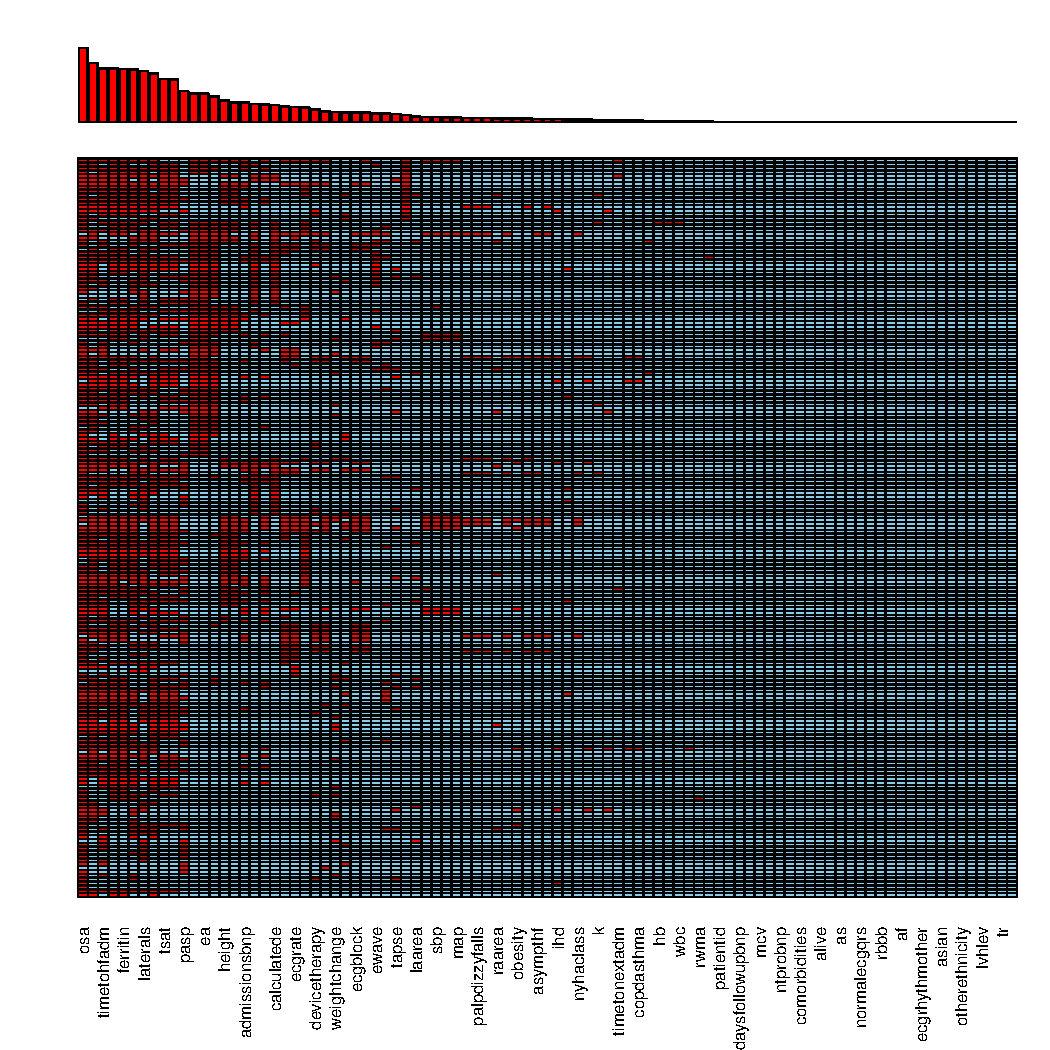
\includegraphics[width=1.1\textwidth]{doc/thesis/images/HFpEF_miss_dist.pdf}
    \caption[Missing values in HFpEF data set]{\textit{Missing values in HFpEF data set. Top:  the amount of missing values in each variable sorted in ascending order. Bottom: plot of the combinations of missing (red) and non-missing (blue) values in the HFpEF data set.}}
    \label{fig:HFpEF_missing}
\end{figure}

\newpage

\begin{figure}[h!]
    \centering
    \hspace*{-1cm}\resizebox{1.1\textwidth}{!}{\footnotesize% Created by tikzDevice version 0.11 on 2018-07-23 18:48:33
% !TEX encoding = UTF-8 Unicode
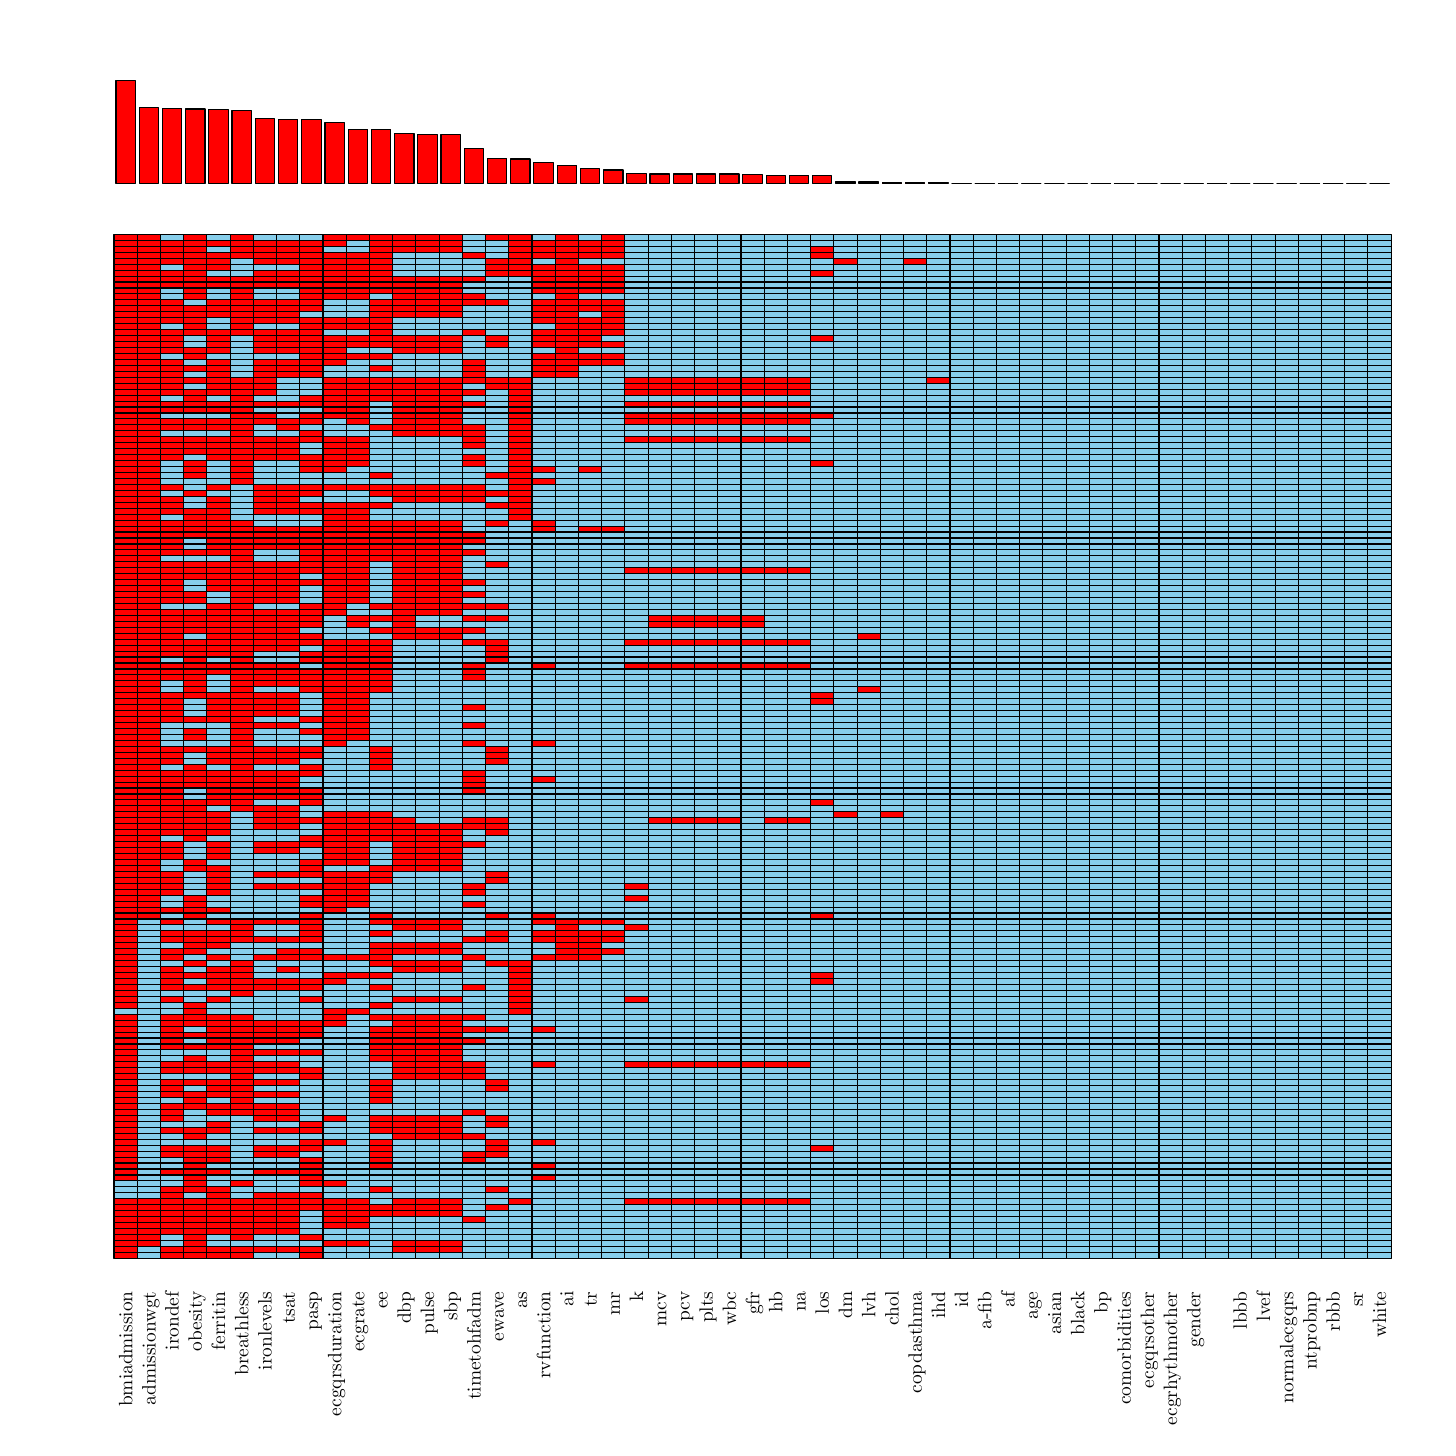
\begin{tikzpicture}[x=1pt,y=1pt]
\definecolor{fillColor}{RGB}{255,255,255}
\path[use as bounding box,fill=fillColor,fill opacity=0.00] (0,0) rectangle (505.89,505.89);
\begin{scope}
\path[clip] (  0.00,  0.00) rectangle (505.89,505.89);
\definecolor{drawColor}{RGB}{0,0,0}
\definecolor{fillColor}{RGB}{255,0,0}

\path[draw=drawColor,line width= 0.4pt,line join=round,line cap=round,fill=fillColor] ( 31.90,449.69) rectangle ( 38.89,486.69);

\path[draw=drawColor,line width= 0.4pt,line join=round,line cap=round,fill=fillColor] ( 40.29,449.69) rectangle ( 47.28,476.92);

\path[draw=drawColor,line width= 0.4pt,line join=round,line cap=round,fill=fillColor] ( 48.68,449.69) rectangle ( 55.67,476.71);

\path[draw=drawColor,line width= 0.4pt,line join=round,line cap=round,fill=fillColor] ( 57.07,449.69) rectangle ( 64.06,476.50);

\path[draw=drawColor,line width= 0.4pt,line join=round,line cap=round,fill=fillColor] ( 65.46,449.69) rectangle ( 72.45,476.30);

\path[draw=drawColor,line width= 0.4pt,line join=round,line cap=round,fill=fillColor] ( 73.85,449.69) rectangle ( 80.85,476.09);

\path[draw=drawColor,line width= 0.4pt,line join=round,line cap=round,fill=fillColor] ( 82.24,449.69) rectangle ( 89.24,472.97);

\path[draw=drawColor,line width= 0.4pt,line join=round,line cap=round,fill=fillColor] ( 90.63,449.69) rectangle ( 97.63,472.76);

\path[draw=drawColor,line width= 0.4pt,line join=round,line cap=round,fill=fillColor] ( 99.03,449.69) rectangle (106.02,472.56);

\path[draw=drawColor,line width= 0.4pt,line join=round,line cap=round,fill=fillColor] (107.42,449.69) rectangle (114.41,471.52);

\path[draw=drawColor,line width= 0.4pt,line join=round,line cap=round,fill=fillColor] (115.81,449.69) rectangle (122.80,469.23);

\path[draw=drawColor,line width= 0.4pt,line join=round,line cap=round,fill=fillColor] (124.20,449.69) rectangle (131.19,469.23);

\path[draw=drawColor,line width= 0.4pt,line join=round,line cap=round,fill=fillColor] (132.59,449.69) rectangle (139.58,467.77);

\path[draw=drawColor,line width= 0.4pt,line join=round,line cap=round,fill=fillColor] (140.98,449.69) rectangle (147.97,467.15);

\path[draw=drawColor,line width= 0.4pt,line join=round,line cap=round,fill=fillColor] (149.37,449.69) rectangle (156.36,467.15);

\path[draw=drawColor,line width= 0.4pt,line join=round,line cap=round,fill=fillColor] (157.76,449.69) rectangle (164.75,462.16);

\path[draw=drawColor,line width= 0.4pt,line join=round,line cap=round,fill=fillColor] (166.15,449.69) rectangle (173.14,458.63);

\path[draw=drawColor,line width= 0.4pt,line join=round,line cap=round,fill=fillColor] (174.54,449.69) rectangle (181.53,458.42);

\path[draw=drawColor,line width= 0.4pt,line join=round,line cap=round,fill=fillColor] (182.93,449.69) rectangle (189.92,457.17);

\path[draw=drawColor,line width= 0.4pt,line join=round,line cap=round,fill=fillColor] (191.32,449.69) rectangle (198.32,456.13);

\path[draw=drawColor,line width= 0.4pt,line join=round,line cap=round,fill=fillColor] (199.71,449.69) rectangle (206.71,454.89);

\path[draw=drawColor,line width= 0.4pt,line join=round,line cap=round,fill=fillColor] (208.10,449.69) rectangle (215.10,454.47);

\path[draw=drawColor,line width= 0.4pt,line join=round,line cap=round,fill=fillColor] (216.50,449.69) rectangle (223.49,453.22);

\path[draw=drawColor,line width= 0.4pt,line join=round,line cap=round,fill=fillColor] (224.89,449.69) rectangle (231.88,453.02);

\path[draw=drawColor,line width= 0.4pt,line join=round,line cap=round,fill=fillColor] (233.28,449.69) rectangle (240.27,453.02);

\path[draw=drawColor,line width= 0.4pt,line join=round,line cap=round,fill=fillColor] (241.67,449.69) rectangle (248.66,453.02);

\path[draw=drawColor,line width= 0.4pt,line join=round,line cap=round,fill=fillColor] (250.06,449.69) rectangle (257.05,453.02);

\path[draw=drawColor,line width= 0.4pt,line join=round,line cap=round,fill=fillColor] (258.45,449.69) rectangle (265.44,452.81);

\path[draw=drawColor,line width= 0.4pt,line join=round,line cap=round,fill=fillColor] (266.84,449.69) rectangle (273.83,452.60);

\path[draw=drawColor,line width= 0.4pt,line join=round,line cap=round,fill=fillColor] (275.23,449.69) rectangle (282.22,452.60);

\path[draw=drawColor,line width= 0.4pt,line join=round,line cap=round,fill=fillColor] (283.62,449.69) rectangle (290.61,452.39);

\path[draw=drawColor,line width= 0.4pt,line join=round,line cap=round,fill=fillColor] (292.01,449.69) rectangle (299.00,450.11);

\path[draw=drawColor,line width= 0.4pt,line join=round,line cap=round,fill=fillColor] (300.40,449.69) rectangle (307.39,450.11);

\path[draw=drawColor,line width= 0.4pt,line join=round,line cap=round,fill=fillColor] (308.79,449.69) rectangle (315.79,449.90);

\path[draw=drawColor,line width= 0.4pt,line join=round,line cap=round,fill=fillColor] (317.18,449.69) rectangle (324.18,449.90);

\path[draw=drawColor,line width= 0.4pt,line join=round,line cap=round,fill=fillColor] (325.57,449.69) rectangle (332.57,449.90);

\path[draw=drawColor,line width= 0.4pt,line join=round,line cap=round,fill=fillColor] (333.97,449.69) rectangle (340.96,449.69);

\path[draw=drawColor,line width= 0.4pt,line join=round,line cap=round,fill=fillColor] (342.36,449.69) rectangle (349.35,449.69);

\path[draw=drawColor,line width= 0.4pt,line join=round,line cap=round,fill=fillColor] (350.75,449.69) rectangle (357.74,449.69);

\path[draw=drawColor,line width= 0.4pt,line join=round,line cap=round,fill=fillColor] (359.14,449.69) rectangle (366.13,449.69);

\path[draw=drawColor,line width= 0.4pt,line join=round,line cap=round,fill=fillColor] (367.53,449.69) rectangle (374.52,449.69);

\path[draw=drawColor,line width= 0.4pt,line join=round,line cap=round,fill=fillColor] (375.92,449.69) rectangle (382.91,449.69);

\path[draw=drawColor,line width= 0.4pt,line join=round,line cap=round,fill=fillColor] (384.31,449.69) rectangle (391.30,449.69);

\path[draw=drawColor,line width= 0.4pt,line join=round,line cap=round,fill=fillColor] (392.70,449.69) rectangle (399.69,449.69);

\path[draw=drawColor,line width= 0.4pt,line join=round,line cap=round,fill=fillColor] (401.09,449.69) rectangle (408.08,449.69);

\path[draw=drawColor,line width= 0.4pt,line join=round,line cap=round,fill=fillColor] (409.48,449.69) rectangle (416.47,449.69);

\path[draw=drawColor,line width= 0.4pt,line join=round,line cap=round,fill=fillColor] (417.87,449.69) rectangle (424.86,449.69);

\path[draw=drawColor,line width= 0.4pt,line join=round,line cap=round,fill=fillColor] (426.26,449.69) rectangle (433.26,449.69);

\path[draw=drawColor,line width= 0.4pt,line join=round,line cap=round,fill=fillColor] (434.65,449.69) rectangle (441.65,449.69);

\path[draw=drawColor,line width= 0.4pt,line join=round,line cap=round,fill=fillColor] (443.04,449.69) rectangle (450.04,449.69);

\path[draw=drawColor,line width= 0.4pt,line join=round,line cap=round,fill=fillColor] (451.44,449.69) rectangle (458.43,449.69);

\path[draw=drawColor,line width= 0.4pt,line join=round,line cap=round,fill=fillColor] (459.83,449.69) rectangle (466.82,449.69);

\path[draw=drawColor,line width= 0.4pt,line join=round,line cap=round,fill=fillColor] (468.22,449.69) rectangle (475.21,449.69);

\path[draw=drawColor,line width= 0.4pt,line join=round,line cap=round,fill=fillColor] (476.61,449.69) rectangle (483.60,449.69);

\path[draw=drawColor,line width= 0.4pt,line join=round,line cap=round,fill=fillColor] (485.00,449.69) rectangle (491.99,449.69);
\end{scope}
\begin{scope}
\path[clip] (  0.00,  0.00) rectangle (505.89,505.89);
\definecolor{drawColor}{RGB}{0,0,0}
\definecolor{fillColor}{RGB}{255,0,0}

\path[draw=drawColor,line width= 0.4pt,line join=round,line cap=round,fill=fillColor] ( 31.20, 61.20) rectangle ( 39.59, 63.35);

\path[draw=drawColor,line width= 0.4pt,line join=round,line cap=round,fill=fillColor] ( 31.20, 63.35) rectangle ( 39.59, 65.50);

\path[draw=drawColor,line width= 0.4pt,line join=round,line cap=round,fill=fillColor] ( 31.20, 65.50) rectangle ( 39.59, 67.65);

\path[draw=drawColor,line width= 0.4pt,line join=round,line cap=round,fill=fillColor] ( 31.20, 67.65) rectangle ( 39.59, 69.80);

\path[draw=drawColor,line width= 0.4pt,line join=round,line cap=round,fill=fillColor] ( 31.20, 69.80) rectangle ( 39.59, 71.96);

\path[draw=drawColor,line width= 0.4pt,line join=round,line cap=round,fill=fillColor] ( 31.20, 71.96) rectangle ( 39.59, 74.11);

\path[draw=drawColor,line width= 0.4pt,line join=round,line cap=round,fill=fillColor] ( 31.20, 74.11) rectangle ( 39.59, 76.26);

\path[draw=drawColor,line width= 0.4pt,line join=round,line cap=round,fill=fillColor] ( 31.20, 76.26) rectangle ( 39.59, 78.41);

\path[draw=drawColor,line width= 0.4pt,line join=round,line cap=round,fill=fillColor] ( 31.20, 78.41) rectangle ( 39.59, 80.56);

\path[draw=drawColor,line width= 0.4pt,line join=round,line cap=round,fill=fillColor] ( 31.20, 80.56) rectangle ( 39.59, 82.71);
\definecolor{fillColor}{RGB}{135,206,235}

\path[draw=drawColor,line width= 0.4pt,line join=round,line cap=round,fill=fillColor] ( 31.20, 82.71) rectangle ( 39.59, 84.86);

\path[draw=drawColor,line width= 0.4pt,line join=round,line cap=round,fill=fillColor] ( 31.20, 84.86) rectangle ( 39.59, 87.01);

\path[draw=drawColor,line width= 0.4pt,line join=round,line cap=round,fill=fillColor] ( 31.20, 87.01) rectangle ( 39.59, 89.16);
\definecolor{fillColor}{RGB}{255,0,0}

\path[draw=drawColor,line width= 0.4pt,line join=round,line cap=round,fill=fillColor] ( 31.20, 89.16) rectangle ( 39.59, 91.32);

\path[draw=drawColor,line width= 0.4pt,line join=round,line cap=round,fill=fillColor] ( 31.20, 91.32) rectangle ( 39.59, 93.47);

\path[draw=drawColor,line width= 0.4pt,line join=round,line cap=round,fill=fillColor] ( 31.20, 93.47) rectangle ( 39.59, 95.62);

\path[draw=drawColor,line width= 0.4pt,line join=round,line cap=round,fill=fillColor] ( 31.20, 95.62) rectangle ( 39.59, 97.77);

\path[draw=drawColor,line width= 0.4pt,line join=round,line cap=round,fill=fillColor] ( 31.20, 97.77) rectangle ( 39.59, 99.92);

\path[draw=drawColor,line width= 0.4pt,line join=round,line cap=round,fill=fillColor] ( 31.20, 99.92) rectangle ( 39.59,102.07);

\path[draw=drawColor,line width= 0.4pt,line join=round,line cap=round,fill=fillColor] ( 31.20,102.07) rectangle ( 39.59,104.22);

\path[draw=drawColor,line width= 0.4pt,line join=round,line cap=round,fill=fillColor] ( 31.20,104.22) rectangle ( 39.59,106.37);

\path[draw=drawColor,line width= 0.4pt,line join=round,line cap=round,fill=fillColor] ( 31.20,106.37) rectangle ( 39.59,108.52);

\path[draw=drawColor,line width= 0.4pt,line join=round,line cap=round,fill=fillColor] ( 31.20,108.52) rectangle ( 39.59,110.68);

\path[draw=drawColor,line width= 0.4pt,line join=round,line cap=round,fill=fillColor] ( 31.20,110.68) rectangle ( 39.59,112.83);

\path[draw=drawColor,line width= 0.4pt,line join=round,line cap=round,fill=fillColor] ( 31.20,112.83) rectangle ( 39.59,114.98);

\path[draw=drawColor,line width= 0.4pt,line join=round,line cap=round,fill=fillColor] ( 31.20,114.98) rectangle ( 39.59,117.13);

\path[draw=drawColor,line width= 0.4pt,line join=round,line cap=round,fill=fillColor] ( 31.20,117.13) rectangle ( 39.59,119.28);

\path[draw=drawColor,line width= 0.4pt,line join=round,line cap=round,fill=fillColor] ( 31.20,119.28) rectangle ( 39.59,121.43);

\path[draw=drawColor,line width= 0.4pt,line join=round,line cap=round,fill=fillColor] ( 31.20,121.43) rectangle ( 39.59,123.58);

\path[draw=drawColor,line width= 0.4pt,line join=round,line cap=round,fill=fillColor] ( 31.20,123.58) rectangle ( 39.59,125.73);

\path[draw=drawColor,line width= 0.4pt,line join=round,line cap=round,fill=fillColor] ( 31.20,125.73) rectangle ( 39.59,127.88);

\path[draw=drawColor,line width= 0.4pt,line join=round,line cap=round,fill=fillColor] ( 31.20,127.88) rectangle ( 39.59,130.04);

\path[draw=drawColor,line width= 0.4pt,line join=round,line cap=round,fill=fillColor] ( 31.20,130.04) rectangle ( 39.59,132.19);

\path[draw=drawColor,line width= 0.4pt,line join=round,line cap=round,fill=fillColor] ( 31.20,132.19) rectangle ( 39.59,134.34);

\path[draw=drawColor,line width= 0.4pt,line join=round,line cap=round,fill=fillColor] ( 31.20,134.34) rectangle ( 39.59,136.49);

\path[draw=drawColor,line width= 0.4pt,line join=round,line cap=round,fill=fillColor] ( 31.20,136.49) rectangle ( 39.59,138.64);

\path[draw=drawColor,line width= 0.4pt,line join=round,line cap=round,fill=fillColor] ( 31.20,138.64) rectangle ( 39.59,140.79);

\path[draw=drawColor,line width= 0.4pt,line join=round,line cap=round,fill=fillColor] ( 31.20,140.79) rectangle ( 39.59,142.94);

\path[draw=drawColor,line width= 0.4pt,line join=round,line cap=round,fill=fillColor] ( 31.20,142.94) rectangle ( 39.59,145.09);

\path[draw=drawColor,line width= 0.4pt,line join=round,line cap=round,fill=fillColor] ( 31.20,145.09) rectangle ( 39.59,147.24);

\path[draw=drawColor,line width= 0.4pt,line join=round,line cap=round,fill=fillColor] ( 31.20,147.24) rectangle ( 39.59,149.40);
\definecolor{fillColor}{RGB}{135,206,235}

\path[draw=drawColor,line width= 0.4pt,line join=round,line cap=round,fill=fillColor] ( 31.20,149.40) rectangle ( 39.59,151.55);
\definecolor{fillColor}{RGB}{255,0,0}

\path[draw=drawColor,line width= 0.4pt,line join=round,line cap=round,fill=fillColor] ( 31.20,151.55) rectangle ( 39.59,153.70);

\path[draw=drawColor,line width= 0.4pt,line join=round,line cap=round,fill=fillColor] ( 31.20,153.70) rectangle ( 39.59,155.85);

\path[draw=drawColor,line width= 0.4pt,line join=round,line cap=round,fill=fillColor] ( 31.20,155.85) rectangle ( 39.59,158.00);

\path[draw=drawColor,line width= 0.4pt,line join=round,line cap=round,fill=fillColor] ( 31.20,158.00) rectangle ( 39.59,160.15);

\path[draw=drawColor,line width= 0.4pt,line join=round,line cap=round,fill=fillColor] ( 31.20,160.15) rectangle ( 39.59,162.30);

\path[draw=drawColor,line width= 0.4pt,line join=round,line cap=round,fill=fillColor] ( 31.20,162.30) rectangle ( 39.59,164.45);

\path[draw=drawColor,line width= 0.4pt,line join=round,line cap=round,fill=fillColor] ( 31.20,164.45) rectangle ( 39.59,166.60);

\path[draw=drawColor,line width= 0.4pt,line join=round,line cap=round,fill=fillColor] ( 31.20,166.60) rectangle ( 39.59,168.76);

\path[draw=drawColor,line width= 0.4pt,line join=round,line cap=round,fill=fillColor] ( 31.20,168.76) rectangle ( 39.59,170.91);

\path[draw=drawColor,line width= 0.4pt,line join=round,line cap=round,fill=fillColor] ( 31.20,170.91) rectangle ( 39.59,173.06);

\path[draw=drawColor,line width= 0.4pt,line join=round,line cap=round,fill=fillColor] ( 31.20,173.06) rectangle ( 39.59,175.21);

\path[draw=drawColor,line width= 0.4pt,line join=round,line cap=round,fill=fillColor] ( 31.20,175.21) rectangle ( 39.59,177.36);

\path[draw=drawColor,line width= 0.4pt,line join=round,line cap=round,fill=fillColor] ( 31.20,177.36) rectangle ( 39.59,179.51);

\path[draw=drawColor,line width= 0.4pt,line join=round,line cap=round,fill=fillColor] ( 31.20,179.51) rectangle ( 39.59,181.66);

\path[draw=drawColor,line width= 0.4pt,line join=round,line cap=round,fill=fillColor] ( 31.20,181.66) rectangle ( 39.59,183.81);

\path[draw=drawColor,line width= 0.4pt,line join=round,line cap=round,fill=fillColor] ( 31.20,183.81) rectangle ( 39.59,185.96);

\path[draw=drawColor,line width= 0.4pt,line join=round,line cap=round,fill=fillColor] ( 31.20,185.96) rectangle ( 39.59,188.12);

\path[draw=drawColor,line width= 0.4pt,line join=round,line cap=round,fill=fillColor] ( 31.20,188.12) rectangle ( 39.59,190.27);

\path[draw=drawColor,line width= 0.4pt,line join=round,line cap=round,fill=fillColor] ( 31.20,190.27) rectangle ( 39.59,192.42);

\path[draw=drawColor,line width= 0.4pt,line join=round,line cap=round,fill=fillColor] ( 31.20,192.42) rectangle ( 39.59,194.57);

\path[draw=drawColor,line width= 0.4pt,line join=round,line cap=round,fill=fillColor] ( 31.20,194.57) rectangle ( 39.59,196.72);

\path[draw=drawColor,line width= 0.4pt,line join=round,line cap=round,fill=fillColor] ( 31.20,196.72) rectangle ( 39.59,198.87);

\path[draw=drawColor,line width= 0.4pt,line join=round,line cap=round,fill=fillColor] ( 31.20,198.87) rectangle ( 39.59,201.02);

\path[draw=drawColor,line width= 0.4pt,line join=round,line cap=round,fill=fillColor] ( 31.20,201.02) rectangle ( 39.59,203.17);

\path[draw=drawColor,line width= 0.4pt,line join=round,line cap=round,fill=fillColor] ( 31.20,203.17) rectangle ( 39.59,205.32);

\path[draw=drawColor,line width= 0.4pt,line join=round,line cap=round,fill=fillColor] ( 31.20,205.32) rectangle ( 39.59,207.48);

\path[draw=drawColor,line width= 0.4pt,line join=round,line cap=round,fill=fillColor] ( 31.20,207.48) rectangle ( 39.59,209.63);

\path[draw=drawColor,line width= 0.4pt,line join=round,line cap=round,fill=fillColor] ( 31.20,209.63) rectangle ( 39.59,211.78);

\path[draw=drawColor,line width= 0.4pt,line join=round,line cap=round,fill=fillColor] ( 31.20,211.78) rectangle ( 39.59,213.93);

\path[draw=drawColor,line width= 0.4pt,line join=round,line cap=round,fill=fillColor] ( 31.20,213.93) rectangle ( 39.59,216.08);

\path[draw=drawColor,line width= 0.4pt,line join=round,line cap=round,fill=fillColor] ( 31.20,216.08) rectangle ( 39.59,218.23);

\path[draw=drawColor,line width= 0.4pt,line join=round,line cap=round,fill=fillColor] ( 31.20,218.23) rectangle ( 39.59,220.38);

\path[draw=drawColor,line width= 0.4pt,line join=round,line cap=round,fill=fillColor] ( 31.20,220.38) rectangle ( 39.59,222.53);

\path[draw=drawColor,line width= 0.4pt,line join=round,line cap=round,fill=fillColor] ( 31.20,222.53) rectangle ( 39.59,224.68);

\path[draw=drawColor,line width= 0.4pt,line join=round,line cap=round,fill=fillColor] ( 31.20,224.68) rectangle ( 39.59,226.84);

\path[draw=drawColor,line width= 0.4pt,line join=round,line cap=round,fill=fillColor] ( 31.20,226.84) rectangle ( 39.59,228.99);

\path[draw=drawColor,line width= 0.4pt,line join=round,line cap=round,fill=fillColor] ( 31.20,228.99) rectangle ( 39.59,231.14);

\path[draw=drawColor,line width= 0.4pt,line join=round,line cap=round,fill=fillColor] ( 31.20,231.14) rectangle ( 39.59,233.29);

\path[draw=drawColor,line width= 0.4pt,line join=round,line cap=round,fill=fillColor] ( 31.20,233.29) rectangle ( 39.59,235.44);

\path[draw=drawColor,line width= 0.4pt,line join=round,line cap=round,fill=fillColor] ( 31.20,235.44) rectangle ( 39.59,237.59);

\path[draw=drawColor,line width= 0.4pt,line join=round,line cap=round,fill=fillColor] ( 31.20,237.59) rectangle ( 39.59,239.74);

\path[draw=drawColor,line width= 0.4pt,line join=round,line cap=round,fill=fillColor] ( 31.20,239.74) rectangle ( 39.59,241.89);

\path[draw=drawColor,line width= 0.4pt,line join=round,line cap=round,fill=fillColor] ( 31.20,241.89) rectangle ( 39.59,244.04);

\path[draw=drawColor,line width= 0.4pt,line join=round,line cap=round,fill=fillColor] ( 31.20,244.04) rectangle ( 39.59,246.20);

\path[draw=drawColor,line width= 0.4pt,line join=round,line cap=round,fill=fillColor] ( 31.20,246.20) rectangle ( 39.59,248.35);

\path[draw=drawColor,line width= 0.4pt,line join=round,line cap=round,fill=fillColor] ( 31.20,248.35) rectangle ( 39.59,250.50);

\path[draw=drawColor,line width= 0.4pt,line join=round,line cap=round,fill=fillColor] ( 31.20,250.50) rectangle ( 39.59,252.65);

\path[draw=drawColor,line width= 0.4pt,line join=round,line cap=round,fill=fillColor] ( 31.20,252.65) rectangle ( 39.59,254.80);

\path[draw=drawColor,line width= 0.4pt,line join=round,line cap=round,fill=fillColor] ( 31.20,254.80) rectangle ( 39.59,256.95);

\path[draw=drawColor,line width= 0.4pt,line join=round,line cap=round,fill=fillColor] ( 31.20,256.95) rectangle ( 39.59,259.10);

\path[draw=drawColor,line width= 0.4pt,line join=round,line cap=round,fill=fillColor] ( 31.20,259.10) rectangle ( 39.59,261.25);

\path[draw=drawColor,line width= 0.4pt,line join=round,line cap=round,fill=fillColor] ( 31.20,261.25) rectangle ( 39.59,263.40);

\path[draw=drawColor,line width= 0.4pt,line join=round,line cap=round,fill=fillColor] ( 31.20,263.40) rectangle ( 39.59,265.56);

\path[draw=drawColor,line width= 0.4pt,line join=round,line cap=round,fill=fillColor] ( 31.20,265.56) rectangle ( 39.59,267.71);

\path[draw=drawColor,line width= 0.4pt,line join=round,line cap=round,fill=fillColor] ( 31.20,267.71) rectangle ( 39.59,269.86);

\path[draw=drawColor,line width= 0.4pt,line join=round,line cap=round,fill=fillColor] ( 31.20,269.86) rectangle ( 39.59,272.01);

\path[draw=drawColor,line width= 0.4pt,line join=round,line cap=round,fill=fillColor] ( 31.20,272.01) rectangle ( 39.59,274.16);

\path[draw=drawColor,line width= 0.4pt,line join=round,line cap=round,fill=fillColor] ( 31.20,274.16) rectangle ( 39.59,276.31);

\path[draw=drawColor,line width= 0.4pt,line join=round,line cap=round,fill=fillColor] ( 31.20,276.31) rectangle ( 39.59,278.46);

\path[draw=drawColor,line width= 0.4pt,line join=round,line cap=round,fill=fillColor] ( 31.20,278.46) rectangle ( 39.59,280.61);

\path[draw=drawColor,line width= 0.4pt,line join=round,line cap=round,fill=fillColor] ( 31.20,280.61) rectangle ( 39.59,282.76);

\path[draw=drawColor,line width= 0.4pt,line join=round,line cap=round,fill=fillColor] ( 31.20,282.76) rectangle ( 39.59,284.92);

\path[draw=drawColor,line width= 0.4pt,line join=round,line cap=round,fill=fillColor] ( 31.20,284.92) rectangle ( 39.59,287.07);

\path[draw=drawColor,line width= 0.4pt,line join=round,line cap=round,fill=fillColor] ( 31.20,287.07) rectangle ( 39.59,289.22);

\path[draw=drawColor,line width= 0.4pt,line join=round,line cap=round,fill=fillColor] ( 31.20,289.22) rectangle ( 39.59,291.37);

\path[draw=drawColor,line width= 0.4pt,line join=round,line cap=round,fill=fillColor] ( 31.20,291.37) rectangle ( 39.59,293.52);

\path[draw=drawColor,line width= 0.4pt,line join=round,line cap=round,fill=fillColor] ( 31.20,293.52) rectangle ( 39.59,295.67);

\path[draw=drawColor,line width= 0.4pt,line join=round,line cap=round,fill=fillColor] ( 31.20,295.67) rectangle ( 39.59,297.82);

\path[draw=drawColor,line width= 0.4pt,line join=round,line cap=round,fill=fillColor] ( 31.20,297.82) rectangle ( 39.59,299.97);

\path[draw=drawColor,line width= 0.4pt,line join=round,line cap=round,fill=fillColor] ( 31.20,299.97) rectangle ( 39.59,302.12);

\path[draw=drawColor,line width= 0.4pt,line join=round,line cap=round,fill=fillColor] ( 31.20,302.12) rectangle ( 39.59,304.28);

\path[draw=drawColor,line width= 0.4pt,line join=round,line cap=round,fill=fillColor] ( 31.20,304.28) rectangle ( 39.59,306.43);

\path[draw=drawColor,line width= 0.4pt,line join=round,line cap=round,fill=fillColor] ( 31.20,306.43) rectangle ( 39.59,308.58);

\path[draw=drawColor,line width= 0.4pt,line join=round,line cap=round,fill=fillColor] ( 31.20,308.58) rectangle ( 39.59,310.73);

\path[draw=drawColor,line width= 0.4pt,line join=round,line cap=round,fill=fillColor] ( 31.20,310.73) rectangle ( 39.59,312.88);

\path[draw=drawColor,line width= 0.4pt,line join=round,line cap=round,fill=fillColor] ( 31.20,312.88) rectangle ( 39.59,315.03);

\path[draw=drawColor,line width= 0.4pt,line join=round,line cap=round,fill=fillColor] ( 31.20,315.03) rectangle ( 39.59,317.18);

\path[draw=drawColor,line width= 0.4pt,line join=round,line cap=round,fill=fillColor] ( 31.20,317.18) rectangle ( 39.59,319.33);

\path[draw=drawColor,line width= 0.4pt,line join=round,line cap=round,fill=fillColor] ( 31.20,319.33) rectangle ( 39.59,321.48);

\path[draw=drawColor,line width= 0.4pt,line join=round,line cap=round,fill=fillColor] ( 31.20,321.48) rectangle ( 39.59,323.64);

\path[draw=drawColor,line width= 0.4pt,line join=round,line cap=round,fill=fillColor] ( 31.20,323.64) rectangle ( 39.59,325.79);

\path[draw=drawColor,line width= 0.4pt,line join=round,line cap=round,fill=fillColor] ( 31.20,325.79) rectangle ( 39.59,327.94);

\path[draw=drawColor,line width= 0.4pt,line join=round,line cap=round,fill=fillColor] ( 31.20,327.94) rectangle ( 39.59,330.09);

\path[draw=drawColor,line width= 0.4pt,line join=round,line cap=round,fill=fillColor] ( 31.20,330.09) rectangle ( 39.59,332.24);

\path[draw=drawColor,line width= 0.4pt,line join=round,line cap=round,fill=fillColor] ( 31.20,332.24) rectangle ( 39.59,334.39);

\path[draw=drawColor,line width= 0.4pt,line join=round,line cap=round,fill=fillColor] ( 31.20,334.39) rectangle ( 39.59,336.54);

\path[draw=drawColor,line width= 0.4pt,line join=round,line cap=round,fill=fillColor] ( 31.20,336.54) rectangle ( 39.59,338.69);

\path[draw=drawColor,line width= 0.4pt,line join=round,line cap=round,fill=fillColor] ( 31.20,338.69) rectangle ( 39.59,340.84);

\path[draw=drawColor,line width= 0.4pt,line join=round,line cap=round,fill=fillColor] ( 31.20,340.84) rectangle ( 39.59,343.00);

\path[draw=drawColor,line width= 0.4pt,line join=round,line cap=round,fill=fillColor] ( 31.20,343.00) rectangle ( 39.59,345.15);

\path[draw=drawColor,line width= 0.4pt,line join=round,line cap=round,fill=fillColor] ( 31.20,345.15) rectangle ( 39.59,347.30);

\path[draw=drawColor,line width= 0.4pt,line join=round,line cap=round,fill=fillColor] ( 31.20,347.30) rectangle ( 39.59,349.45);

\path[draw=drawColor,line width= 0.4pt,line join=round,line cap=round,fill=fillColor] ( 31.20,349.45) rectangle ( 39.59,351.60);

\path[draw=drawColor,line width= 0.4pt,line join=round,line cap=round,fill=fillColor] ( 31.20,351.60) rectangle ( 39.59,353.75);

\path[draw=drawColor,line width= 0.4pt,line join=round,line cap=round,fill=fillColor] ( 31.20,353.75) rectangle ( 39.59,355.90);

\path[draw=drawColor,line width= 0.4pt,line join=round,line cap=round,fill=fillColor] ( 31.20,355.90) rectangle ( 39.59,358.05);

\path[draw=drawColor,line width= 0.4pt,line join=round,line cap=round,fill=fillColor] ( 31.20,358.05) rectangle ( 39.59,360.20);

\path[draw=drawColor,line width= 0.4pt,line join=round,line cap=round,fill=fillColor] ( 31.20,360.20) rectangle ( 39.59,362.36);

\path[draw=drawColor,line width= 0.4pt,line join=round,line cap=round,fill=fillColor] ( 31.20,362.36) rectangle ( 39.59,364.51);

\path[draw=drawColor,line width= 0.4pt,line join=round,line cap=round,fill=fillColor] ( 31.20,364.51) rectangle ( 39.59,366.66);

\path[draw=drawColor,line width= 0.4pt,line join=round,line cap=round,fill=fillColor] ( 31.20,366.66) rectangle ( 39.59,368.81);

\path[draw=drawColor,line width= 0.4pt,line join=round,line cap=round,fill=fillColor] ( 31.20,368.81) rectangle ( 39.59,370.96);

\path[draw=drawColor,line width= 0.4pt,line join=round,line cap=round,fill=fillColor] ( 31.20,370.96) rectangle ( 39.59,373.11);

\path[draw=drawColor,line width= 0.4pt,line join=round,line cap=round,fill=fillColor] ( 31.20,373.11) rectangle ( 39.59,375.26);

\path[draw=drawColor,line width= 0.4pt,line join=round,line cap=round,fill=fillColor] ( 31.20,375.26) rectangle ( 39.59,377.41);

\path[draw=drawColor,line width= 0.4pt,line join=round,line cap=round,fill=fillColor] ( 31.20,377.41) rectangle ( 39.59,379.56);

\path[draw=drawColor,line width= 0.4pt,line join=round,line cap=round,fill=fillColor] ( 31.20,379.56) rectangle ( 39.59,381.72);

\path[draw=drawColor,line width= 0.4pt,line join=round,line cap=round,fill=fillColor] ( 31.20,381.72) rectangle ( 39.59,383.87);

\path[draw=drawColor,line width= 0.4pt,line join=round,line cap=round,fill=fillColor] ( 31.20,383.87) rectangle ( 39.59,386.02);

\path[draw=drawColor,line width= 0.4pt,line join=round,line cap=round,fill=fillColor] ( 31.20,386.02) rectangle ( 39.59,388.17);

\path[draw=drawColor,line width= 0.4pt,line join=round,line cap=round,fill=fillColor] ( 31.20,388.17) rectangle ( 39.59,390.32);

\path[draw=drawColor,line width= 0.4pt,line join=round,line cap=round,fill=fillColor] ( 31.20,390.32) rectangle ( 39.59,392.47);

\path[draw=drawColor,line width= 0.4pt,line join=round,line cap=round,fill=fillColor] ( 31.20,392.47) rectangle ( 39.59,394.62);

\path[draw=drawColor,line width= 0.4pt,line join=round,line cap=round,fill=fillColor] ( 31.20,394.62) rectangle ( 39.59,396.77);

\path[draw=drawColor,line width= 0.4pt,line join=round,line cap=round,fill=fillColor] ( 31.20,396.77) rectangle ( 39.59,398.92);

\path[draw=drawColor,line width= 0.4pt,line join=round,line cap=round,fill=fillColor] ( 31.20,398.92) rectangle ( 39.59,401.08);

\path[draw=drawColor,line width= 0.4pt,line join=round,line cap=round,fill=fillColor] ( 31.20,401.08) rectangle ( 39.59,403.23);

\path[draw=drawColor,line width= 0.4pt,line join=round,line cap=round,fill=fillColor] ( 31.20,403.23) rectangle ( 39.59,405.38);

\path[draw=drawColor,line width= 0.4pt,line join=round,line cap=round,fill=fillColor] ( 31.20,405.38) rectangle ( 39.59,407.53);

\path[draw=drawColor,line width= 0.4pt,line join=round,line cap=round,fill=fillColor] ( 31.20,407.53) rectangle ( 39.59,409.68);

\path[draw=drawColor,line width= 0.4pt,line join=round,line cap=round,fill=fillColor] ( 31.20,409.68) rectangle ( 39.59,411.83);

\path[draw=drawColor,line width= 0.4pt,line join=round,line cap=round,fill=fillColor] ( 31.20,411.83) rectangle ( 39.59,413.98);

\path[draw=drawColor,line width= 0.4pt,line join=round,line cap=round,fill=fillColor] ( 31.20,413.98) rectangle ( 39.59,416.13);

\path[draw=drawColor,line width= 0.4pt,line join=round,line cap=round,fill=fillColor] ( 31.20,416.13) rectangle ( 39.59,418.28);

\path[draw=drawColor,line width= 0.4pt,line join=round,line cap=round,fill=fillColor] ( 31.20,418.28) rectangle ( 39.59,420.44);

\path[draw=drawColor,line width= 0.4pt,line join=round,line cap=round,fill=fillColor] ( 31.20,420.44) rectangle ( 39.59,422.59);

\path[draw=drawColor,line width= 0.4pt,line join=round,line cap=round,fill=fillColor] ( 31.20,422.59) rectangle ( 39.59,424.74);

\path[draw=drawColor,line width= 0.4pt,line join=round,line cap=round,fill=fillColor] ( 31.20,424.74) rectangle ( 39.59,426.89);

\path[draw=drawColor,line width= 0.4pt,line join=round,line cap=round,fill=fillColor] ( 31.20,426.89) rectangle ( 39.59,429.04);

\path[draw=drawColor,line width= 0.4pt,line join=round,line cap=round,fill=fillColor] ( 31.20,429.04) rectangle ( 39.59,431.19);
\definecolor{fillColor}{RGB}{135,206,235}

\path[draw=drawColor,line width= 0.4pt,line join=round,line cap=round,fill=fillColor] ( 39.59, 61.20) rectangle ( 47.98, 63.35);

\path[draw=drawColor,line width= 0.4pt,line join=round,line cap=round,fill=fillColor] ( 39.59, 63.35) rectangle ( 47.98, 65.50);
\definecolor{fillColor}{RGB}{255,0,0}

\path[draw=drawColor,line width= 0.4pt,line join=round,line cap=round,fill=fillColor] ( 39.59, 65.50) rectangle ( 47.98, 67.65);

\path[draw=drawColor,line width= 0.4pt,line join=round,line cap=round,fill=fillColor] ( 39.59, 67.65) rectangle ( 47.98, 69.80);

\path[draw=drawColor,line width= 0.4pt,line join=round,line cap=round,fill=fillColor] ( 39.59, 69.80) rectangle ( 47.98, 71.96);

\path[draw=drawColor,line width= 0.4pt,line join=round,line cap=round,fill=fillColor] ( 39.59, 71.96) rectangle ( 47.98, 74.11);

\path[draw=drawColor,line width= 0.4pt,line join=round,line cap=round,fill=fillColor] ( 39.59, 74.11) rectangle ( 47.98, 76.26);

\path[draw=drawColor,line width= 0.4pt,line join=round,line cap=round,fill=fillColor] ( 39.59, 76.26) rectangle ( 47.98, 78.41);

\path[draw=drawColor,line width= 0.4pt,line join=round,line cap=round,fill=fillColor] ( 39.59, 78.41) rectangle ( 47.98, 80.56);

\path[draw=drawColor,line width= 0.4pt,line join=round,line cap=round,fill=fillColor] ( 39.59, 80.56) rectangle ( 47.98, 82.71);
\definecolor{fillColor}{RGB}{135,206,235}

\path[draw=drawColor,line width= 0.4pt,line join=round,line cap=round,fill=fillColor] ( 39.59, 82.71) rectangle ( 47.98, 84.86);

\path[draw=drawColor,line width= 0.4pt,line join=round,line cap=round,fill=fillColor] ( 39.59, 84.86) rectangle ( 47.98, 87.01);

\path[draw=drawColor,line width= 0.4pt,line join=round,line cap=round,fill=fillColor] ( 39.59, 87.01) rectangle ( 47.98, 89.16);

\path[draw=drawColor,line width= 0.4pt,line join=round,line cap=round,fill=fillColor] ( 39.59, 89.16) rectangle ( 47.98, 91.32);

\path[draw=drawColor,line width= 0.4pt,line join=round,line cap=round,fill=fillColor] ( 39.59, 91.32) rectangle ( 47.98, 93.47);

\path[draw=drawColor,line width= 0.4pt,line join=round,line cap=round,fill=fillColor] ( 39.59, 93.47) rectangle ( 47.98, 95.62);

\path[draw=drawColor,line width= 0.4pt,line join=round,line cap=round,fill=fillColor] ( 39.59, 95.62) rectangle ( 47.98, 97.77);

\path[draw=drawColor,line width= 0.4pt,line join=round,line cap=round,fill=fillColor] ( 39.59, 97.77) rectangle ( 47.98, 99.92);

\path[draw=drawColor,line width= 0.4pt,line join=round,line cap=round,fill=fillColor] ( 39.59, 99.92) rectangle ( 47.98,102.07);

\path[draw=drawColor,line width= 0.4pt,line join=round,line cap=round,fill=fillColor] ( 39.59,102.07) rectangle ( 47.98,104.22);

\path[draw=drawColor,line width= 0.4pt,line join=round,line cap=round,fill=fillColor] ( 39.59,104.22) rectangle ( 47.98,106.37);

\path[draw=drawColor,line width= 0.4pt,line join=round,line cap=round,fill=fillColor] ( 39.59,106.37) rectangle ( 47.98,108.52);

\path[draw=drawColor,line width= 0.4pt,line join=round,line cap=round,fill=fillColor] ( 39.59,108.52) rectangle ( 47.98,110.68);

\path[draw=drawColor,line width= 0.4pt,line join=round,line cap=round,fill=fillColor] ( 39.59,110.68) rectangle ( 47.98,112.83);

\path[draw=drawColor,line width= 0.4pt,line join=round,line cap=round,fill=fillColor] ( 39.59,112.83) rectangle ( 47.98,114.98);

\path[draw=drawColor,line width= 0.4pt,line join=round,line cap=round,fill=fillColor] ( 39.59,114.98) rectangle ( 47.98,117.13);

\path[draw=drawColor,line width= 0.4pt,line join=round,line cap=round,fill=fillColor] ( 39.59,117.13) rectangle ( 47.98,119.28);

\path[draw=drawColor,line width= 0.4pt,line join=round,line cap=round,fill=fillColor] ( 39.59,119.28) rectangle ( 47.98,121.43);

\path[draw=drawColor,line width= 0.4pt,line join=round,line cap=round,fill=fillColor] ( 39.59,121.43) rectangle ( 47.98,123.58);

\path[draw=drawColor,line width= 0.4pt,line join=round,line cap=round,fill=fillColor] ( 39.59,123.58) rectangle ( 47.98,125.73);

\path[draw=drawColor,line width= 0.4pt,line join=round,line cap=round,fill=fillColor] ( 39.59,125.73) rectangle ( 47.98,127.88);

\path[draw=drawColor,line width= 0.4pt,line join=round,line cap=round,fill=fillColor] ( 39.59,127.88) rectangle ( 47.98,130.04);

\path[draw=drawColor,line width= 0.4pt,line join=round,line cap=round,fill=fillColor] ( 39.59,130.04) rectangle ( 47.98,132.19);

\path[draw=drawColor,line width= 0.4pt,line join=round,line cap=round,fill=fillColor] ( 39.59,132.19) rectangle ( 47.98,134.34);

\path[draw=drawColor,line width= 0.4pt,line join=round,line cap=round,fill=fillColor] ( 39.59,134.34) rectangle ( 47.98,136.49);

\path[draw=drawColor,line width= 0.4pt,line join=round,line cap=round,fill=fillColor] ( 39.59,136.49) rectangle ( 47.98,138.64);

\path[draw=drawColor,line width= 0.4pt,line join=round,line cap=round,fill=fillColor] ( 39.59,138.64) rectangle ( 47.98,140.79);

\path[draw=drawColor,line width= 0.4pt,line join=round,line cap=round,fill=fillColor] ( 39.59,140.79) rectangle ( 47.98,142.94);

\path[draw=drawColor,line width= 0.4pt,line join=round,line cap=round,fill=fillColor] ( 39.59,142.94) rectangle ( 47.98,145.09);

\path[draw=drawColor,line width= 0.4pt,line join=round,line cap=round,fill=fillColor] ( 39.59,145.09) rectangle ( 47.98,147.24);

\path[draw=drawColor,line width= 0.4pt,line join=round,line cap=round,fill=fillColor] ( 39.59,147.24) rectangle ( 47.98,149.40);

\path[draw=drawColor,line width= 0.4pt,line join=round,line cap=round,fill=fillColor] ( 39.59,149.40) rectangle ( 47.98,151.55);

\path[draw=drawColor,line width= 0.4pt,line join=round,line cap=round,fill=fillColor] ( 39.59,151.55) rectangle ( 47.98,153.70);

\path[draw=drawColor,line width= 0.4pt,line join=round,line cap=round,fill=fillColor] ( 39.59,153.70) rectangle ( 47.98,155.85);

\path[draw=drawColor,line width= 0.4pt,line join=round,line cap=round,fill=fillColor] ( 39.59,155.85) rectangle ( 47.98,158.00);

\path[draw=drawColor,line width= 0.4pt,line join=round,line cap=round,fill=fillColor] ( 39.59,158.00) rectangle ( 47.98,160.15);

\path[draw=drawColor,line width= 0.4pt,line join=round,line cap=round,fill=fillColor] ( 39.59,160.15) rectangle ( 47.98,162.30);

\path[draw=drawColor,line width= 0.4pt,line join=round,line cap=round,fill=fillColor] ( 39.59,162.30) rectangle ( 47.98,164.45);

\path[draw=drawColor,line width= 0.4pt,line join=round,line cap=round,fill=fillColor] ( 39.59,164.45) rectangle ( 47.98,166.60);

\path[draw=drawColor,line width= 0.4pt,line join=round,line cap=round,fill=fillColor] ( 39.59,166.60) rectangle ( 47.98,168.76);

\path[draw=drawColor,line width= 0.4pt,line join=round,line cap=round,fill=fillColor] ( 39.59,168.76) rectangle ( 47.98,170.91);

\path[draw=drawColor,line width= 0.4pt,line join=round,line cap=round,fill=fillColor] ( 39.59,170.91) rectangle ( 47.98,173.06);

\path[draw=drawColor,line width= 0.4pt,line join=round,line cap=round,fill=fillColor] ( 39.59,173.06) rectangle ( 47.98,175.21);

\path[draw=drawColor,line width= 0.4pt,line join=round,line cap=round,fill=fillColor] ( 39.59,175.21) rectangle ( 47.98,177.36);

\path[draw=drawColor,line width= 0.4pt,line join=round,line cap=round,fill=fillColor] ( 39.59,177.36) rectangle ( 47.98,179.51);

\path[draw=drawColor,line width= 0.4pt,line join=round,line cap=round,fill=fillColor] ( 39.59,179.51) rectangle ( 47.98,181.66);

\path[draw=drawColor,line width= 0.4pt,line join=round,line cap=round,fill=fillColor] ( 39.59,181.66) rectangle ( 47.98,183.81);
\definecolor{fillColor}{RGB}{255,0,0}

\path[draw=drawColor,line width= 0.4pt,line join=round,line cap=round,fill=fillColor] ( 39.59,183.81) rectangle ( 47.98,185.96);

\path[draw=drawColor,line width= 0.4pt,line join=round,line cap=round,fill=fillColor] ( 39.59,185.96) rectangle ( 47.98,188.12);

\path[draw=drawColor,line width= 0.4pt,line join=round,line cap=round,fill=fillColor] ( 39.59,188.12) rectangle ( 47.98,190.27);

\path[draw=drawColor,line width= 0.4pt,line join=round,line cap=round,fill=fillColor] ( 39.59,190.27) rectangle ( 47.98,192.42);

\path[draw=drawColor,line width= 0.4pt,line join=round,line cap=round,fill=fillColor] ( 39.59,192.42) rectangle ( 47.98,194.57);

\path[draw=drawColor,line width= 0.4pt,line join=round,line cap=round,fill=fillColor] ( 39.59,194.57) rectangle ( 47.98,196.72);

\path[draw=drawColor,line width= 0.4pt,line join=round,line cap=round,fill=fillColor] ( 39.59,196.72) rectangle ( 47.98,198.87);

\path[draw=drawColor,line width= 0.4pt,line join=round,line cap=round,fill=fillColor] ( 39.59,198.87) rectangle ( 47.98,201.02);

\path[draw=drawColor,line width= 0.4pt,line join=round,line cap=round,fill=fillColor] ( 39.59,201.02) rectangle ( 47.98,203.17);

\path[draw=drawColor,line width= 0.4pt,line join=round,line cap=round,fill=fillColor] ( 39.59,203.17) rectangle ( 47.98,205.32);

\path[draw=drawColor,line width= 0.4pt,line join=round,line cap=round,fill=fillColor] ( 39.59,205.32) rectangle ( 47.98,207.48);

\path[draw=drawColor,line width= 0.4pt,line join=round,line cap=round,fill=fillColor] ( 39.59,207.48) rectangle ( 47.98,209.63);

\path[draw=drawColor,line width= 0.4pt,line join=round,line cap=round,fill=fillColor] ( 39.59,209.63) rectangle ( 47.98,211.78);

\path[draw=drawColor,line width= 0.4pt,line join=round,line cap=round,fill=fillColor] ( 39.59,211.78) rectangle ( 47.98,213.93);

\path[draw=drawColor,line width= 0.4pt,line join=round,line cap=round,fill=fillColor] ( 39.59,213.93) rectangle ( 47.98,216.08);

\path[draw=drawColor,line width= 0.4pt,line join=round,line cap=round,fill=fillColor] ( 39.59,216.08) rectangle ( 47.98,218.23);

\path[draw=drawColor,line width= 0.4pt,line join=round,line cap=round,fill=fillColor] ( 39.59,218.23) rectangle ( 47.98,220.38);

\path[draw=drawColor,line width= 0.4pt,line join=round,line cap=round,fill=fillColor] ( 39.59,220.38) rectangle ( 47.98,222.53);

\path[draw=drawColor,line width= 0.4pt,line join=round,line cap=round,fill=fillColor] ( 39.59,222.53) rectangle ( 47.98,224.68);

\path[draw=drawColor,line width= 0.4pt,line join=round,line cap=round,fill=fillColor] ( 39.59,224.68) rectangle ( 47.98,226.84);

\path[draw=drawColor,line width= 0.4pt,line join=round,line cap=round,fill=fillColor] ( 39.59,226.84) rectangle ( 47.98,228.99);

\path[draw=drawColor,line width= 0.4pt,line join=round,line cap=round,fill=fillColor] ( 39.59,228.99) rectangle ( 47.98,231.14);

\path[draw=drawColor,line width= 0.4pt,line join=round,line cap=round,fill=fillColor] ( 39.59,231.14) rectangle ( 47.98,233.29);

\path[draw=drawColor,line width= 0.4pt,line join=round,line cap=round,fill=fillColor] ( 39.59,233.29) rectangle ( 47.98,235.44);

\path[draw=drawColor,line width= 0.4pt,line join=round,line cap=round,fill=fillColor] ( 39.59,235.44) rectangle ( 47.98,237.59);

\path[draw=drawColor,line width= 0.4pt,line join=round,line cap=round,fill=fillColor] ( 39.59,237.59) rectangle ( 47.98,239.74);

\path[draw=drawColor,line width= 0.4pt,line join=round,line cap=round,fill=fillColor] ( 39.59,239.74) rectangle ( 47.98,241.89);

\path[draw=drawColor,line width= 0.4pt,line join=round,line cap=round,fill=fillColor] ( 39.59,241.89) rectangle ( 47.98,244.04);

\path[draw=drawColor,line width= 0.4pt,line join=round,line cap=round,fill=fillColor] ( 39.59,244.04) rectangle ( 47.98,246.20);

\path[draw=drawColor,line width= 0.4pt,line join=round,line cap=round,fill=fillColor] ( 39.59,246.20) rectangle ( 47.98,248.35);

\path[draw=drawColor,line width= 0.4pt,line join=round,line cap=round,fill=fillColor] ( 39.59,248.35) rectangle ( 47.98,250.50);

\path[draw=drawColor,line width= 0.4pt,line join=round,line cap=round,fill=fillColor] ( 39.59,250.50) rectangle ( 47.98,252.65);

\path[draw=drawColor,line width= 0.4pt,line join=round,line cap=round,fill=fillColor] ( 39.59,252.65) rectangle ( 47.98,254.80);

\path[draw=drawColor,line width= 0.4pt,line join=round,line cap=round,fill=fillColor] ( 39.59,254.80) rectangle ( 47.98,256.95);

\path[draw=drawColor,line width= 0.4pt,line join=round,line cap=round,fill=fillColor] ( 39.59,256.95) rectangle ( 47.98,259.10);

\path[draw=drawColor,line width= 0.4pt,line join=round,line cap=round,fill=fillColor] ( 39.59,259.10) rectangle ( 47.98,261.25);

\path[draw=drawColor,line width= 0.4pt,line join=round,line cap=round,fill=fillColor] ( 39.59,261.25) rectangle ( 47.98,263.40);

\path[draw=drawColor,line width= 0.4pt,line join=round,line cap=round,fill=fillColor] ( 39.59,263.40) rectangle ( 47.98,265.56);

\path[draw=drawColor,line width= 0.4pt,line join=round,line cap=round,fill=fillColor] ( 39.59,265.56) rectangle ( 47.98,267.71);

\path[draw=drawColor,line width= 0.4pt,line join=round,line cap=round,fill=fillColor] ( 39.59,267.71) rectangle ( 47.98,269.86);

\path[draw=drawColor,line width= 0.4pt,line join=round,line cap=round,fill=fillColor] ( 39.59,269.86) rectangle ( 47.98,272.01);

\path[draw=drawColor,line width= 0.4pt,line join=round,line cap=round,fill=fillColor] ( 39.59,272.01) rectangle ( 47.98,274.16);

\path[draw=drawColor,line width= 0.4pt,line join=round,line cap=round,fill=fillColor] ( 39.59,274.16) rectangle ( 47.98,276.31);

\path[draw=drawColor,line width= 0.4pt,line join=round,line cap=round,fill=fillColor] ( 39.59,276.31) rectangle ( 47.98,278.46);

\path[draw=drawColor,line width= 0.4pt,line join=round,line cap=round,fill=fillColor] ( 39.59,278.46) rectangle ( 47.98,280.61);

\path[draw=drawColor,line width= 0.4pt,line join=round,line cap=round,fill=fillColor] ( 39.59,280.61) rectangle ( 47.98,282.76);

\path[draw=drawColor,line width= 0.4pt,line join=round,line cap=round,fill=fillColor] ( 39.59,282.76) rectangle ( 47.98,284.92);

\path[draw=drawColor,line width= 0.4pt,line join=round,line cap=round,fill=fillColor] ( 39.59,284.92) rectangle ( 47.98,287.07);

\path[draw=drawColor,line width= 0.4pt,line join=round,line cap=round,fill=fillColor] ( 39.59,287.07) rectangle ( 47.98,289.22);

\path[draw=drawColor,line width= 0.4pt,line join=round,line cap=round,fill=fillColor] ( 39.59,289.22) rectangle ( 47.98,291.37);

\path[draw=drawColor,line width= 0.4pt,line join=round,line cap=round,fill=fillColor] ( 39.59,291.37) rectangle ( 47.98,293.52);

\path[draw=drawColor,line width= 0.4pt,line join=round,line cap=round,fill=fillColor] ( 39.59,293.52) rectangle ( 47.98,295.67);

\path[draw=drawColor,line width= 0.4pt,line join=round,line cap=round,fill=fillColor] ( 39.59,295.67) rectangle ( 47.98,297.82);

\path[draw=drawColor,line width= 0.4pt,line join=round,line cap=round,fill=fillColor] ( 39.59,297.82) rectangle ( 47.98,299.97);

\path[draw=drawColor,line width= 0.4pt,line join=round,line cap=round,fill=fillColor] ( 39.59,299.97) rectangle ( 47.98,302.12);

\path[draw=drawColor,line width= 0.4pt,line join=round,line cap=round,fill=fillColor] ( 39.59,302.12) rectangle ( 47.98,304.28);

\path[draw=drawColor,line width= 0.4pt,line join=round,line cap=round,fill=fillColor] ( 39.59,304.28) rectangle ( 47.98,306.43);

\path[draw=drawColor,line width= 0.4pt,line join=round,line cap=round,fill=fillColor] ( 39.59,306.43) rectangle ( 47.98,308.58);

\path[draw=drawColor,line width= 0.4pt,line join=round,line cap=round,fill=fillColor] ( 39.59,308.58) rectangle ( 47.98,310.73);

\path[draw=drawColor,line width= 0.4pt,line join=round,line cap=round,fill=fillColor] ( 39.59,310.73) rectangle ( 47.98,312.88);

\path[draw=drawColor,line width= 0.4pt,line join=round,line cap=round,fill=fillColor] ( 39.59,312.88) rectangle ( 47.98,315.03);

\path[draw=drawColor,line width= 0.4pt,line join=round,line cap=round,fill=fillColor] ( 39.59,315.03) rectangle ( 47.98,317.18);

\path[draw=drawColor,line width= 0.4pt,line join=round,line cap=round,fill=fillColor] ( 39.59,317.18) rectangle ( 47.98,319.33);

\path[draw=drawColor,line width= 0.4pt,line join=round,line cap=round,fill=fillColor] ( 39.59,319.33) rectangle ( 47.98,321.48);

\path[draw=drawColor,line width= 0.4pt,line join=round,line cap=round,fill=fillColor] ( 39.59,321.48) rectangle ( 47.98,323.64);

\path[draw=drawColor,line width= 0.4pt,line join=round,line cap=round,fill=fillColor] ( 39.59,323.64) rectangle ( 47.98,325.79);

\path[draw=drawColor,line width= 0.4pt,line join=round,line cap=round,fill=fillColor] ( 39.59,325.79) rectangle ( 47.98,327.94);

\path[draw=drawColor,line width= 0.4pt,line join=round,line cap=round,fill=fillColor] ( 39.59,327.94) rectangle ( 47.98,330.09);

\path[draw=drawColor,line width= 0.4pt,line join=round,line cap=round,fill=fillColor] ( 39.59,330.09) rectangle ( 47.98,332.24);

\path[draw=drawColor,line width= 0.4pt,line join=round,line cap=round,fill=fillColor] ( 39.59,332.24) rectangle ( 47.98,334.39);

\path[draw=drawColor,line width= 0.4pt,line join=round,line cap=round,fill=fillColor] ( 39.59,334.39) rectangle ( 47.98,336.54);

\path[draw=drawColor,line width= 0.4pt,line join=round,line cap=round,fill=fillColor] ( 39.59,336.54) rectangle ( 47.98,338.69);

\path[draw=drawColor,line width= 0.4pt,line join=round,line cap=round,fill=fillColor] ( 39.59,338.69) rectangle ( 47.98,340.84);

\path[draw=drawColor,line width= 0.4pt,line join=round,line cap=round,fill=fillColor] ( 39.59,340.84) rectangle ( 47.98,343.00);

\path[draw=drawColor,line width= 0.4pt,line join=round,line cap=round,fill=fillColor] ( 39.59,343.00) rectangle ( 47.98,345.15);

\path[draw=drawColor,line width= 0.4pt,line join=round,line cap=round,fill=fillColor] ( 39.59,345.15) rectangle ( 47.98,347.30);

\path[draw=drawColor,line width= 0.4pt,line join=round,line cap=round,fill=fillColor] ( 39.59,347.30) rectangle ( 47.98,349.45);

\path[draw=drawColor,line width= 0.4pt,line join=round,line cap=round,fill=fillColor] ( 39.59,349.45) rectangle ( 47.98,351.60);

\path[draw=drawColor,line width= 0.4pt,line join=round,line cap=round,fill=fillColor] ( 39.59,351.60) rectangle ( 47.98,353.75);

\path[draw=drawColor,line width= 0.4pt,line join=round,line cap=round,fill=fillColor] ( 39.59,353.75) rectangle ( 47.98,355.90);

\path[draw=drawColor,line width= 0.4pt,line join=round,line cap=round,fill=fillColor] ( 39.59,355.90) rectangle ( 47.98,358.05);

\path[draw=drawColor,line width= 0.4pt,line join=round,line cap=round,fill=fillColor] ( 39.59,358.05) rectangle ( 47.98,360.20);

\path[draw=drawColor,line width= 0.4pt,line join=round,line cap=round,fill=fillColor] ( 39.59,360.20) rectangle ( 47.98,362.36);

\path[draw=drawColor,line width= 0.4pt,line join=round,line cap=round,fill=fillColor] ( 39.59,362.36) rectangle ( 47.98,364.51);

\path[draw=drawColor,line width= 0.4pt,line join=round,line cap=round,fill=fillColor] ( 39.59,364.51) rectangle ( 47.98,366.66);

\path[draw=drawColor,line width= 0.4pt,line join=round,line cap=round,fill=fillColor] ( 39.59,366.66) rectangle ( 47.98,368.81);

\path[draw=drawColor,line width= 0.4pt,line join=round,line cap=round,fill=fillColor] ( 39.59,368.81) rectangle ( 47.98,370.96);

\path[draw=drawColor,line width= 0.4pt,line join=round,line cap=round,fill=fillColor] ( 39.59,370.96) rectangle ( 47.98,373.11);

\path[draw=drawColor,line width= 0.4pt,line join=round,line cap=round,fill=fillColor] ( 39.59,373.11) rectangle ( 47.98,375.26);

\path[draw=drawColor,line width= 0.4pt,line join=round,line cap=round,fill=fillColor] ( 39.59,375.26) rectangle ( 47.98,377.41);

\path[draw=drawColor,line width= 0.4pt,line join=round,line cap=round,fill=fillColor] ( 39.59,377.41) rectangle ( 47.98,379.56);

\path[draw=drawColor,line width= 0.4pt,line join=round,line cap=round,fill=fillColor] ( 39.59,379.56) rectangle ( 47.98,381.72);

\path[draw=drawColor,line width= 0.4pt,line join=round,line cap=round,fill=fillColor] ( 39.59,381.72) rectangle ( 47.98,383.87);

\path[draw=drawColor,line width= 0.4pt,line join=round,line cap=round,fill=fillColor] ( 39.59,383.87) rectangle ( 47.98,386.02);

\path[draw=drawColor,line width= 0.4pt,line join=round,line cap=round,fill=fillColor] ( 39.59,386.02) rectangle ( 47.98,388.17);

\path[draw=drawColor,line width= 0.4pt,line join=round,line cap=round,fill=fillColor] ( 39.59,388.17) rectangle ( 47.98,390.32);

\path[draw=drawColor,line width= 0.4pt,line join=round,line cap=round,fill=fillColor] ( 39.59,390.32) rectangle ( 47.98,392.47);

\path[draw=drawColor,line width= 0.4pt,line join=round,line cap=round,fill=fillColor] ( 39.59,392.47) rectangle ( 47.98,394.62);

\path[draw=drawColor,line width= 0.4pt,line join=round,line cap=round,fill=fillColor] ( 39.59,394.62) rectangle ( 47.98,396.77);

\path[draw=drawColor,line width= 0.4pt,line join=round,line cap=round,fill=fillColor] ( 39.59,396.77) rectangle ( 47.98,398.92);

\path[draw=drawColor,line width= 0.4pt,line join=round,line cap=round,fill=fillColor] ( 39.59,398.92) rectangle ( 47.98,401.08);

\path[draw=drawColor,line width= 0.4pt,line join=round,line cap=round,fill=fillColor] ( 39.59,401.08) rectangle ( 47.98,403.23);

\path[draw=drawColor,line width= 0.4pt,line join=round,line cap=round,fill=fillColor] ( 39.59,403.23) rectangle ( 47.98,405.38);

\path[draw=drawColor,line width= 0.4pt,line join=round,line cap=round,fill=fillColor] ( 39.59,405.38) rectangle ( 47.98,407.53);

\path[draw=drawColor,line width= 0.4pt,line join=round,line cap=round,fill=fillColor] ( 39.59,407.53) rectangle ( 47.98,409.68);

\path[draw=drawColor,line width= 0.4pt,line join=round,line cap=round,fill=fillColor] ( 39.59,409.68) rectangle ( 47.98,411.83);

\path[draw=drawColor,line width= 0.4pt,line join=round,line cap=round,fill=fillColor] ( 39.59,411.83) rectangle ( 47.98,413.98);

\path[draw=drawColor,line width= 0.4pt,line join=round,line cap=round,fill=fillColor] ( 39.59,413.98) rectangle ( 47.98,416.13);

\path[draw=drawColor,line width= 0.4pt,line join=round,line cap=round,fill=fillColor] ( 39.59,416.13) rectangle ( 47.98,418.28);

\path[draw=drawColor,line width= 0.4pt,line join=round,line cap=round,fill=fillColor] ( 39.59,418.28) rectangle ( 47.98,420.44);

\path[draw=drawColor,line width= 0.4pt,line join=round,line cap=round,fill=fillColor] ( 39.59,420.44) rectangle ( 47.98,422.59);

\path[draw=drawColor,line width= 0.4pt,line join=round,line cap=round,fill=fillColor] ( 39.59,422.59) rectangle ( 47.98,424.74);

\path[draw=drawColor,line width= 0.4pt,line join=round,line cap=round,fill=fillColor] ( 39.59,424.74) rectangle ( 47.98,426.89);

\path[draw=drawColor,line width= 0.4pt,line join=round,line cap=round,fill=fillColor] ( 39.59,426.89) rectangle ( 47.98,429.04);

\path[draw=drawColor,line width= 0.4pt,line join=round,line cap=round,fill=fillColor] ( 39.59,429.04) rectangle ( 47.98,431.19);

\path[draw=drawColor,line width= 0.4pt,line join=round,line cap=round,fill=fillColor] ( 47.98, 61.20) rectangle ( 56.37, 63.35);

\path[draw=drawColor,line width= 0.4pt,line join=round,line cap=round,fill=fillColor] ( 47.98, 63.35) rectangle ( 56.37, 65.50);
\definecolor{fillColor}{RGB}{135,206,235}

\path[draw=drawColor,line width= 0.4pt,line join=round,line cap=round,fill=fillColor] ( 47.98, 65.50) rectangle ( 56.37, 67.65);

\path[draw=drawColor,line width= 0.4pt,line join=round,line cap=round,fill=fillColor] ( 47.98, 67.65) rectangle ( 56.37, 69.80);
\definecolor{fillColor}{RGB}{255,0,0}

\path[draw=drawColor,line width= 0.4pt,line join=round,line cap=round,fill=fillColor] ( 47.98, 69.80) rectangle ( 56.37, 71.96);

\path[draw=drawColor,line width= 0.4pt,line join=round,line cap=round,fill=fillColor] ( 47.98, 71.96) rectangle ( 56.37, 74.11);

\path[draw=drawColor,line width= 0.4pt,line join=round,line cap=round,fill=fillColor] ( 47.98, 74.11) rectangle ( 56.37, 76.26);

\path[draw=drawColor,line width= 0.4pt,line join=round,line cap=round,fill=fillColor] ( 47.98, 76.26) rectangle ( 56.37, 78.41);

\path[draw=drawColor,line width= 0.4pt,line join=round,line cap=round,fill=fillColor] ( 47.98, 78.41) rectangle ( 56.37, 80.56);

\path[draw=drawColor,line width= 0.4pt,line join=round,line cap=round,fill=fillColor] ( 47.98, 80.56) rectangle ( 56.37, 82.71);

\path[draw=drawColor,line width= 0.4pt,line join=round,line cap=round,fill=fillColor] ( 47.98, 82.71) rectangle ( 56.37, 84.86);

\path[draw=drawColor,line width= 0.4pt,line join=round,line cap=round,fill=fillColor] ( 47.98, 84.86) rectangle ( 56.37, 87.01);
\definecolor{fillColor}{RGB}{135,206,235}

\path[draw=drawColor,line width= 0.4pt,line join=round,line cap=round,fill=fillColor] ( 47.98, 87.01) rectangle ( 56.37, 89.16);

\path[draw=drawColor,line width= 0.4pt,line join=round,line cap=round,fill=fillColor] ( 47.98, 89.16) rectangle ( 56.37, 91.32);
\definecolor{fillColor}{RGB}{255,0,0}

\path[draw=drawColor,line width= 0.4pt,line join=round,line cap=round,fill=fillColor] ( 47.98, 91.32) rectangle ( 56.37, 93.47);
\definecolor{fillColor}{RGB}{135,206,235}

\path[draw=drawColor,line width= 0.4pt,line join=round,line cap=round,fill=fillColor] ( 47.98, 93.47) rectangle ( 56.37, 95.62);

\path[draw=drawColor,line width= 0.4pt,line join=round,line cap=round,fill=fillColor] ( 47.98, 95.62) rectangle ( 56.37, 97.77);
\definecolor{fillColor}{RGB}{255,0,0}

\path[draw=drawColor,line width= 0.4pt,line join=round,line cap=round,fill=fillColor] ( 47.98, 97.77) rectangle ( 56.37, 99.92);

\path[draw=drawColor,line width= 0.4pt,line join=round,line cap=round,fill=fillColor] ( 47.98, 99.92) rectangle ( 56.37,102.07);
\definecolor{fillColor}{RGB}{135,206,235}

\path[draw=drawColor,line width= 0.4pt,line join=round,line cap=round,fill=fillColor] ( 47.98,102.07) rectangle ( 56.37,104.22);

\path[draw=drawColor,line width= 0.4pt,line join=round,line cap=round,fill=fillColor] ( 47.98,104.22) rectangle ( 56.37,106.37);
\definecolor{fillColor}{RGB}{255,0,0}

\path[draw=drawColor,line width= 0.4pt,line join=round,line cap=round,fill=fillColor] ( 47.98,106.37) rectangle ( 56.37,108.52);
\definecolor{fillColor}{RGB}{135,206,235}

\path[draw=drawColor,line width= 0.4pt,line join=round,line cap=round,fill=fillColor] ( 47.98,108.52) rectangle ( 56.37,110.68);
\definecolor{fillColor}{RGB}{255,0,0}

\path[draw=drawColor,line width= 0.4pt,line join=round,line cap=round,fill=fillColor] ( 47.98,110.68) rectangle ( 56.37,112.83);

\path[draw=drawColor,line width= 0.4pt,line join=round,line cap=round,fill=fillColor] ( 47.98,112.83) rectangle ( 56.37,114.98);

\path[draw=drawColor,line width= 0.4pt,line join=round,line cap=round,fill=fillColor] ( 47.98,114.98) rectangle ( 56.37,117.13);
\definecolor{fillColor}{RGB}{135,206,235}

\path[draw=drawColor,line width= 0.4pt,line join=round,line cap=round,fill=fillColor] ( 47.98,117.13) rectangle ( 56.37,119.28);
\definecolor{fillColor}{RGB}{255,0,0}

\path[draw=drawColor,line width= 0.4pt,line join=round,line cap=round,fill=fillColor] ( 47.98,119.28) rectangle ( 56.37,121.43);

\path[draw=drawColor,line width= 0.4pt,line join=round,line cap=round,fill=fillColor] ( 47.98,121.43) rectangle ( 56.37,123.58);

\path[draw=drawColor,line width= 0.4pt,line join=round,line cap=round,fill=fillColor] ( 47.98,123.58) rectangle ( 56.37,125.73);
\definecolor{fillColor}{RGB}{135,206,235}

\path[draw=drawColor,line width= 0.4pt,line join=round,line cap=round,fill=fillColor] ( 47.98,125.73) rectangle ( 56.37,127.88);
\definecolor{fillColor}{RGB}{255,0,0}

\path[draw=drawColor,line width= 0.4pt,line join=round,line cap=round,fill=fillColor] ( 47.98,127.88) rectangle ( 56.37,130.04);

\path[draw=drawColor,line width= 0.4pt,line join=round,line cap=round,fill=fillColor] ( 47.98,130.04) rectangle ( 56.37,132.19);
\definecolor{fillColor}{RGB}{135,206,235}

\path[draw=drawColor,line width= 0.4pt,line join=round,line cap=round,fill=fillColor] ( 47.98,132.19) rectangle ( 56.37,134.34);

\path[draw=drawColor,line width= 0.4pt,line join=round,line cap=round,fill=fillColor] ( 47.98,134.34) rectangle ( 56.37,136.49);
\definecolor{fillColor}{RGB}{255,0,0}

\path[draw=drawColor,line width= 0.4pt,line join=round,line cap=round,fill=fillColor] ( 47.98,136.49) rectangle ( 56.37,138.64);

\path[draw=drawColor,line width= 0.4pt,line join=round,line cap=round,fill=fillColor] ( 47.98,138.64) rectangle ( 56.37,140.79);

\path[draw=drawColor,line width= 0.4pt,line join=round,line cap=round,fill=fillColor] ( 47.98,140.79) rectangle ( 56.37,142.94);

\path[draw=drawColor,line width= 0.4pt,line join=round,line cap=round,fill=fillColor] ( 47.98,142.94) rectangle ( 56.37,145.09);

\path[draw=drawColor,line width= 0.4pt,line join=round,line cap=round,fill=fillColor] ( 47.98,145.09) rectangle ( 56.37,147.24);

\path[draw=drawColor,line width= 0.4pt,line join=round,line cap=round,fill=fillColor] ( 47.98,147.24) rectangle ( 56.37,149.40);
\definecolor{fillColor}{RGB}{135,206,235}

\path[draw=drawColor,line width= 0.4pt,line join=round,line cap=round,fill=fillColor] ( 47.98,149.40) rectangle ( 56.37,151.55);

\path[draw=drawColor,line width= 0.4pt,line join=round,line cap=round,fill=fillColor] ( 47.98,151.55) rectangle ( 56.37,153.70);
\definecolor{fillColor}{RGB}{255,0,0}

\path[draw=drawColor,line width= 0.4pt,line join=round,line cap=round,fill=fillColor] ( 47.98,153.70) rectangle ( 56.37,155.85);
\definecolor{fillColor}{RGB}{135,206,235}

\path[draw=drawColor,line width= 0.4pt,line join=round,line cap=round,fill=fillColor] ( 47.98,155.85) rectangle ( 56.37,158.00);
\definecolor{fillColor}{RGB}{255,0,0}

\path[draw=drawColor,line width= 0.4pt,line join=round,line cap=round,fill=fillColor] ( 47.98,158.00) rectangle ( 56.37,160.15);

\path[draw=drawColor,line width= 0.4pt,line join=round,line cap=round,fill=fillColor] ( 47.98,160.15) rectangle ( 56.37,162.30);

\path[draw=drawColor,line width= 0.4pt,line join=round,line cap=round,fill=fillColor] ( 47.98,162.30) rectangle ( 56.37,164.45);

\path[draw=drawColor,line width= 0.4pt,line join=round,line cap=round,fill=fillColor] ( 47.98,164.45) rectangle ( 56.37,166.60);
\definecolor{fillColor}{RGB}{135,206,235}

\path[draw=drawColor,line width= 0.4pt,line join=round,line cap=round,fill=fillColor] ( 47.98,166.60) rectangle ( 56.37,168.76);
\definecolor{fillColor}{RGB}{255,0,0}

\path[draw=drawColor,line width= 0.4pt,line join=round,line cap=round,fill=fillColor] ( 47.98,168.76) rectangle ( 56.37,170.91);

\path[draw=drawColor,line width= 0.4pt,line join=round,line cap=round,fill=fillColor] ( 47.98,170.91) rectangle ( 56.37,173.06);
\definecolor{fillColor}{RGB}{135,206,235}

\path[draw=drawColor,line width= 0.4pt,line join=round,line cap=round,fill=fillColor] ( 47.98,173.06) rectangle ( 56.37,175.21);
\definecolor{fillColor}{RGB}{255,0,0}

\path[draw=drawColor,line width= 0.4pt,line join=round,line cap=round,fill=fillColor] ( 47.98,175.21) rectangle ( 56.37,177.36);

\path[draw=drawColor,line width= 0.4pt,line join=round,line cap=round,fill=fillColor] ( 47.98,177.36) rectangle ( 56.37,179.51);
\definecolor{fillColor}{RGB}{135,206,235}

\path[draw=drawColor,line width= 0.4pt,line join=round,line cap=round,fill=fillColor] ( 47.98,179.51) rectangle ( 56.37,181.66);
\definecolor{fillColor}{RGB}{255,0,0}

\path[draw=drawColor,line width= 0.4pt,line join=round,line cap=round,fill=fillColor] ( 47.98,181.66) rectangle ( 56.37,183.81);
\definecolor{fillColor}{RGB}{135,206,235}

\path[draw=drawColor,line width= 0.4pt,line join=round,line cap=round,fill=fillColor] ( 47.98,183.81) rectangle ( 56.37,185.96);
\definecolor{fillColor}{RGB}{255,0,0}

\path[draw=drawColor,line width= 0.4pt,line join=round,line cap=round,fill=fillColor] ( 47.98,185.96) rectangle ( 56.37,188.12);
\definecolor{fillColor}{RGB}{135,206,235}

\path[draw=drawColor,line width= 0.4pt,line join=round,line cap=round,fill=fillColor] ( 47.98,188.12) rectangle ( 56.37,190.27);

\path[draw=drawColor,line width= 0.4pt,line join=round,line cap=round,fill=fillColor] ( 47.98,190.27) rectangle ( 56.37,192.42);
\definecolor{fillColor}{RGB}{255,0,0}

\path[draw=drawColor,line width= 0.4pt,line join=round,line cap=round,fill=fillColor] ( 47.98,192.42) rectangle ( 56.37,194.57);

\path[draw=drawColor,line width= 0.4pt,line join=round,line cap=round,fill=fillColor] ( 47.98,194.57) rectangle ( 56.37,196.72);

\path[draw=drawColor,line width= 0.4pt,line join=round,line cap=round,fill=fillColor] ( 47.98,196.72) rectangle ( 56.37,198.87);

\path[draw=drawColor,line width= 0.4pt,line join=round,line cap=round,fill=fillColor] ( 47.98,198.87) rectangle ( 56.37,201.02);
\definecolor{fillColor}{RGB}{135,206,235}

\path[draw=drawColor,line width= 0.4pt,line join=round,line cap=round,fill=fillColor] ( 47.98,201.02) rectangle ( 56.37,203.17);

\path[draw=drawColor,line width= 0.4pt,line join=round,line cap=round,fill=fillColor] ( 47.98,203.17) rectangle ( 56.37,205.32);
\definecolor{fillColor}{RGB}{255,0,0}

\path[draw=drawColor,line width= 0.4pt,line join=round,line cap=round,fill=fillColor] ( 47.98,205.32) rectangle ( 56.37,207.48);

\path[draw=drawColor,line width= 0.4pt,line join=round,line cap=round,fill=fillColor] ( 47.98,207.48) rectangle ( 56.37,209.63);

\path[draw=drawColor,line width= 0.4pt,line join=round,line cap=round,fill=fillColor] ( 47.98,209.63) rectangle ( 56.37,211.78);
\definecolor{fillColor}{RGB}{135,206,235}

\path[draw=drawColor,line width= 0.4pt,line join=round,line cap=round,fill=fillColor] ( 47.98,211.78) rectangle ( 56.37,213.93);
\definecolor{fillColor}{RGB}{255,0,0}

\path[draw=drawColor,line width= 0.4pt,line join=round,line cap=round,fill=fillColor] ( 47.98,213.93) rectangle ( 56.37,216.08);

\path[draw=drawColor,line width= 0.4pt,line join=round,line cap=round,fill=fillColor] ( 47.98,216.08) rectangle ( 56.37,218.23);

\path[draw=drawColor,line width= 0.4pt,line join=round,line cap=round,fill=fillColor] ( 47.98,218.23) rectangle ( 56.37,220.38);

\path[draw=drawColor,line width= 0.4pt,line join=round,line cap=round,fill=fillColor] ( 47.98,220.38) rectangle ( 56.37,222.53);

\path[draw=drawColor,line width= 0.4pt,line join=round,line cap=round,fill=fillColor] ( 47.98,222.53) rectangle ( 56.37,224.68);

\path[draw=drawColor,line width= 0.4pt,line join=round,line cap=round,fill=fillColor] ( 47.98,224.68) rectangle ( 56.37,226.84);

\path[draw=drawColor,line width= 0.4pt,line join=round,line cap=round,fill=fillColor] ( 47.98,226.84) rectangle ( 56.37,228.99);

\path[draw=drawColor,line width= 0.4pt,line join=round,line cap=round,fill=fillColor] ( 47.98,228.99) rectangle ( 56.37,231.14);

\path[draw=drawColor,line width= 0.4pt,line join=round,line cap=round,fill=fillColor] ( 47.98,231.14) rectangle ( 56.37,233.29);

\path[draw=drawColor,line width= 0.4pt,line join=round,line cap=round,fill=fillColor] ( 47.98,233.29) rectangle ( 56.37,235.44);

\path[draw=drawColor,line width= 0.4pt,line join=round,line cap=round,fill=fillColor] ( 47.98,235.44) rectangle ( 56.37,237.59);
\definecolor{fillColor}{RGB}{135,206,235}

\path[draw=drawColor,line width= 0.4pt,line join=round,line cap=round,fill=fillColor] ( 47.98,237.59) rectangle ( 56.37,239.74);
\definecolor{fillColor}{RGB}{255,0,0}

\path[draw=drawColor,line width= 0.4pt,line join=round,line cap=round,fill=fillColor] ( 47.98,239.74) rectangle ( 56.37,241.89);

\path[draw=drawColor,line width= 0.4pt,line join=round,line cap=round,fill=fillColor] ( 47.98,241.89) rectangle ( 56.37,244.04);

\path[draw=drawColor,line width= 0.4pt,line join=round,line cap=round,fill=fillColor] ( 47.98,244.04) rectangle ( 56.37,246.20);
\definecolor{fillColor}{RGB}{135,206,235}

\path[draw=drawColor,line width= 0.4pt,line join=round,line cap=round,fill=fillColor] ( 47.98,246.20) rectangle ( 56.37,248.35);

\path[draw=drawColor,line width= 0.4pt,line join=round,line cap=round,fill=fillColor] ( 47.98,248.35) rectangle ( 56.37,250.50);

\path[draw=drawColor,line width= 0.4pt,line join=round,line cap=round,fill=fillColor] ( 47.98,250.50) rectangle ( 56.37,252.65);

\path[draw=drawColor,line width= 0.4pt,line join=round,line cap=round,fill=fillColor] ( 47.98,252.65) rectangle ( 56.37,254.80);
\definecolor{fillColor}{RGB}{255,0,0}

\path[draw=drawColor,line width= 0.4pt,line join=round,line cap=round,fill=fillColor] ( 47.98,254.80) rectangle ( 56.37,256.95);

\path[draw=drawColor,line width= 0.4pt,line join=round,line cap=round,fill=fillColor] ( 47.98,256.95) rectangle ( 56.37,259.10);

\path[draw=drawColor,line width= 0.4pt,line join=round,line cap=round,fill=fillColor] ( 47.98,259.10) rectangle ( 56.37,261.25);

\path[draw=drawColor,line width= 0.4pt,line join=round,line cap=round,fill=fillColor] ( 47.98,261.25) rectangle ( 56.37,263.40);

\path[draw=drawColor,line width= 0.4pt,line join=round,line cap=round,fill=fillColor] ( 47.98,263.40) rectangle ( 56.37,265.56);
\definecolor{fillColor}{RGB}{135,206,235}

\path[draw=drawColor,line width= 0.4pt,line join=round,line cap=round,fill=fillColor] ( 47.98,265.56) rectangle ( 56.37,267.71);

\path[draw=drawColor,line width= 0.4pt,line join=round,line cap=round,fill=fillColor] ( 47.98,267.71) rectangle ( 56.37,269.86);
\definecolor{fillColor}{RGB}{255,0,0}

\path[draw=drawColor,line width= 0.4pt,line join=round,line cap=round,fill=fillColor] ( 47.98,269.86) rectangle ( 56.37,272.01);

\path[draw=drawColor,line width= 0.4pt,line join=round,line cap=round,fill=fillColor] ( 47.98,272.01) rectangle ( 56.37,274.16);

\path[draw=drawColor,line width= 0.4pt,line join=round,line cap=round,fill=fillColor] ( 47.98,274.16) rectangle ( 56.37,276.31);
\definecolor{fillColor}{RGB}{135,206,235}

\path[draw=drawColor,line width= 0.4pt,line join=round,line cap=round,fill=fillColor] ( 47.98,276.31) rectangle ( 56.37,278.46);
\definecolor{fillColor}{RGB}{255,0,0}

\path[draw=drawColor,line width= 0.4pt,line join=round,line cap=round,fill=fillColor] ( 47.98,278.46) rectangle ( 56.37,280.61);

\path[draw=drawColor,line width= 0.4pt,line join=round,line cap=round,fill=fillColor] ( 47.98,280.61) rectangle ( 56.37,282.76);

\path[draw=drawColor,line width= 0.4pt,line join=round,line cap=round,fill=fillColor] ( 47.98,282.76) rectangle ( 56.37,284.92);

\path[draw=drawColor,line width= 0.4pt,line join=round,line cap=round,fill=fillColor] ( 47.98,284.92) rectangle ( 56.37,287.07);

\path[draw=drawColor,line width= 0.4pt,line join=round,line cap=round,fill=fillColor] ( 47.98,287.07) rectangle ( 56.37,289.22);

\path[draw=drawColor,line width= 0.4pt,line join=round,line cap=round,fill=fillColor] ( 47.98,289.22) rectangle ( 56.37,291.37);

\path[draw=drawColor,line width= 0.4pt,line join=round,line cap=round,fill=fillColor] ( 47.98,291.37) rectangle ( 56.37,293.52);

\path[draw=drawColor,line width= 0.4pt,line join=round,line cap=round,fill=fillColor] ( 47.98,293.52) rectangle ( 56.37,295.67);
\definecolor{fillColor}{RGB}{135,206,235}

\path[draw=drawColor,line width= 0.4pt,line join=round,line cap=round,fill=fillColor] ( 47.98,295.67) rectangle ( 56.37,297.82);
\definecolor{fillColor}{RGB}{255,0,0}

\path[draw=drawColor,line width= 0.4pt,line join=round,line cap=round,fill=fillColor] ( 47.98,297.82) rectangle ( 56.37,299.97);

\path[draw=drawColor,line width= 0.4pt,line join=round,line cap=round,fill=fillColor] ( 47.98,299.97) rectangle ( 56.37,302.12);

\path[draw=drawColor,line width= 0.4pt,line join=round,line cap=round,fill=fillColor] ( 47.98,302.12) rectangle ( 56.37,304.28);

\path[draw=drawColor,line width= 0.4pt,line join=round,line cap=round,fill=fillColor] ( 47.98,304.28) rectangle ( 56.37,306.43);

\path[draw=drawColor,line width= 0.4pt,line join=round,line cap=round,fill=fillColor] ( 47.98,306.43) rectangle ( 56.37,308.58);

\path[draw=drawColor,line width= 0.4pt,line join=round,line cap=round,fill=fillColor] ( 47.98,308.58) rectangle ( 56.37,310.73);

\path[draw=drawColor,line width= 0.4pt,line join=round,line cap=round,fill=fillColor] ( 47.98,310.73) rectangle ( 56.37,312.88);
\definecolor{fillColor}{RGB}{135,206,235}

\path[draw=drawColor,line width= 0.4pt,line join=round,line cap=round,fill=fillColor] ( 47.98,312.88) rectangle ( 56.37,315.03);
\definecolor{fillColor}{RGB}{255,0,0}

\path[draw=drawColor,line width= 0.4pt,line join=round,line cap=round,fill=fillColor] ( 47.98,315.03) rectangle ( 56.37,317.18);

\path[draw=drawColor,line width= 0.4pt,line join=round,line cap=round,fill=fillColor] ( 47.98,317.18) rectangle ( 56.37,319.33);

\path[draw=drawColor,line width= 0.4pt,line join=round,line cap=round,fill=fillColor] ( 47.98,319.33) rectangle ( 56.37,321.48);

\path[draw=drawColor,line width= 0.4pt,line join=round,line cap=round,fill=fillColor] ( 47.98,321.48) rectangle ( 56.37,323.64);

\path[draw=drawColor,line width= 0.4pt,line join=round,line cap=round,fill=fillColor] ( 47.98,323.64) rectangle ( 56.37,325.79);

\path[draw=drawColor,line width= 0.4pt,line join=round,line cap=round,fill=fillColor] ( 47.98,325.79) rectangle ( 56.37,327.94);
\definecolor{fillColor}{RGB}{135,206,235}

\path[draw=drawColor,line width= 0.4pt,line join=round,line cap=round,fill=fillColor] ( 47.98,327.94) rectangle ( 56.37,330.09);
\definecolor{fillColor}{RGB}{255,0,0}

\path[draw=drawColor,line width= 0.4pt,line join=round,line cap=round,fill=fillColor] ( 47.98,330.09) rectangle ( 56.37,332.24);

\path[draw=drawColor,line width= 0.4pt,line join=round,line cap=round,fill=fillColor] ( 47.98,332.24) rectangle ( 56.37,334.39);

\path[draw=drawColor,line width= 0.4pt,line join=round,line cap=round,fill=fillColor] ( 47.98,334.39) rectangle ( 56.37,336.54);
\definecolor{fillColor}{RGB}{135,206,235}

\path[draw=drawColor,line width= 0.4pt,line join=round,line cap=round,fill=fillColor] ( 47.98,336.54) rectangle ( 56.37,338.69);
\definecolor{fillColor}{RGB}{255,0,0}

\path[draw=drawColor,line width= 0.4pt,line join=round,line cap=round,fill=fillColor] ( 47.98,338.69) rectangle ( 56.37,340.84);
\definecolor{fillColor}{RGB}{135,206,235}

\path[draw=drawColor,line width= 0.4pt,line join=round,line cap=round,fill=fillColor] ( 47.98,340.84) rectangle ( 56.37,343.00);

\path[draw=drawColor,line width= 0.4pt,line join=round,line cap=round,fill=fillColor] ( 47.98,343.00) rectangle ( 56.37,345.15);

\path[draw=drawColor,line width= 0.4pt,line join=round,line cap=round,fill=fillColor] ( 47.98,345.15) rectangle ( 56.37,347.30);

\path[draw=drawColor,line width= 0.4pt,line join=round,line cap=round,fill=fillColor] ( 47.98,347.30) rectangle ( 56.37,349.45);
\definecolor{fillColor}{RGB}{255,0,0}

\path[draw=drawColor,line width= 0.4pt,line join=round,line cap=round,fill=fillColor] ( 47.98,349.45) rectangle ( 56.37,351.60);

\path[draw=drawColor,line width= 0.4pt,line join=round,line cap=round,fill=fillColor] ( 47.98,351.60) rectangle ( 56.37,353.75);

\path[draw=drawColor,line width= 0.4pt,line join=round,line cap=round,fill=fillColor] ( 47.98,353.75) rectangle ( 56.37,355.90);

\path[draw=drawColor,line width= 0.4pt,line join=round,line cap=round,fill=fillColor] ( 47.98,355.90) rectangle ( 56.37,358.05);
\definecolor{fillColor}{RGB}{135,206,235}

\path[draw=drawColor,line width= 0.4pt,line join=round,line cap=round,fill=fillColor] ( 47.98,358.05) rectangle ( 56.37,360.20);
\definecolor{fillColor}{RGB}{255,0,0}

\path[draw=drawColor,line width= 0.4pt,line join=round,line cap=round,fill=fillColor] ( 47.98,360.20) rectangle ( 56.37,362.36);

\path[draw=drawColor,line width= 0.4pt,line join=round,line cap=round,fill=fillColor] ( 47.98,362.36) rectangle ( 56.37,364.51);
\definecolor{fillColor}{RGB}{135,206,235}

\path[draw=drawColor,line width= 0.4pt,line join=round,line cap=round,fill=fillColor] ( 47.98,364.51) rectangle ( 56.37,366.66);
\definecolor{fillColor}{RGB}{255,0,0}

\path[draw=drawColor,line width= 0.4pt,line join=round,line cap=round,fill=fillColor] ( 47.98,366.66) rectangle ( 56.37,368.81);

\path[draw=drawColor,line width= 0.4pt,line join=round,line cap=round,fill=fillColor] ( 47.98,368.81) rectangle ( 56.37,370.96);
\definecolor{fillColor}{RGB}{135,206,235}

\path[draw=drawColor,line width= 0.4pt,line join=round,line cap=round,fill=fillColor] ( 47.98,370.96) rectangle ( 56.37,373.11);
\definecolor{fillColor}{RGB}{255,0,0}

\path[draw=drawColor,line width= 0.4pt,line join=round,line cap=round,fill=fillColor] ( 47.98,373.11) rectangle ( 56.37,375.26);

\path[draw=drawColor,line width= 0.4pt,line join=round,line cap=round,fill=fillColor] ( 47.98,375.26) rectangle ( 56.37,377.41);

\path[draw=drawColor,line width= 0.4pt,line join=round,line cap=round,fill=fillColor] ( 47.98,377.41) rectangle ( 56.37,379.56);

\path[draw=drawColor,line width= 0.4pt,line join=round,line cap=round,fill=fillColor] ( 47.98,379.56) rectangle ( 56.37,381.72);

\path[draw=drawColor,line width= 0.4pt,line join=round,line cap=round,fill=fillColor] ( 47.98,381.72) rectangle ( 56.37,383.87);

\path[draw=drawColor,line width= 0.4pt,line join=round,line cap=round,fill=fillColor] ( 47.98,383.87) rectangle ( 56.37,386.02);
\definecolor{fillColor}{RGB}{135,206,235}

\path[draw=drawColor,line width= 0.4pt,line join=round,line cap=round,fill=fillColor] ( 47.98,386.02) rectangle ( 56.37,388.17);
\definecolor{fillColor}{RGB}{255,0,0}

\path[draw=drawColor,line width= 0.4pt,line join=round,line cap=round,fill=fillColor] ( 47.98,388.17) rectangle ( 56.37,390.32);

\path[draw=drawColor,line width= 0.4pt,line join=round,line cap=round,fill=fillColor] ( 47.98,390.32) rectangle ( 56.37,392.47);

\path[draw=drawColor,line width= 0.4pt,line join=round,line cap=round,fill=fillColor] ( 47.98,392.47) rectangle ( 56.37,394.62);

\path[draw=drawColor,line width= 0.4pt,line join=round,line cap=round,fill=fillColor] ( 47.98,394.62) rectangle ( 56.37,396.77);
\definecolor{fillColor}{RGB}{135,206,235}

\path[draw=drawColor,line width= 0.4pt,line join=round,line cap=round,fill=fillColor] ( 47.98,396.77) rectangle ( 56.37,398.92);
\definecolor{fillColor}{RGB}{255,0,0}

\path[draw=drawColor,line width= 0.4pt,line join=round,line cap=round,fill=fillColor] ( 47.98,398.92) rectangle ( 56.37,401.08);

\path[draw=drawColor,line width= 0.4pt,line join=round,line cap=round,fill=fillColor] ( 47.98,401.08) rectangle ( 56.37,403.23);

\path[draw=drawColor,line width= 0.4pt,line join=round,line cap=round,fill=fillColor] ( 47.98,403.23) rectangle ( 56.37,405.38);

\path[draw=drawColor,line width= 0.4pt,line join=round,line cap=round,fill=fillColor] ( 47.98,405.38) rectangle ( 56.37,407.53);
\definecolor{fillColor}{RGB}{135,206,235}

\path[draw=drawColor,line width= 0.4pt,line join=round,line cap=round,fill=fillColor] ( 47.98,407.53) rectangle ( 56.37,409.68);

\path[draw=drawColor,line width= 0.4pt,line join=round,line cap=round,fill=fillColor] ( 47.98,409.68) rectangle ( 56.37,411.83);
\definecolor{fillColor}{RGB}{255,0,0}

\path[draw=drawColor,line width= 0.4pt,line join=round,line cap=round,fill=fillColor] ( 47.98,411.83) rectangle ( 56.37,413.98);

\path[draw=drawColor,line width= 0.4pt,line join=round,line cap=round,fill=fillColor] ( 47.98,413.98) rectangle ( 56.37,416.13);

\path[draw=drawColor,line width= 0.4pt,line join=round,line cap=round,fill=fillColor] ( 47.98,416.13) rectangle ( 56.37,418.28);
\definecolor{fillColor}{RGB}{135,206,235}

\path[draw=drawColor,line width= 0.4pt,line join=round,line cap=round,fill=fillColor] ( 47.98,418.28) rectangle ( 56.37,420.44);
\definecolor{fillColor}{RGB}{255,0,0}

\path[draw=drawColor,line width= 0.4pt,line join=round,line cap=round,fill=fillColor] ( 47.98,420.44) rectangle ( 56.37,422.59);

\path[draw=drawColor,line width= 0.4pt,line join=round,line cap=round,fill=fillColor] ( 47.98,422.59) rectangle ( 56.37,424.74);

\path[draw=drawColor,line width= 0.4pt,line join=round,line cap=round,fill=fillColor] ( 47.98,424.74) rectangle ( 56.37,426.89);

\path[draw=drawColor,line width= 0.4pt,line join=round,line cap=round,fill=fillColor] ( 47.98,426.89) rectangle ( 56.37,429.04);
\definecolor{fillColor}{RGB}{135,206,235}

\path[draw=drawColor,line width= 0.4pt,line join=round,line cap=round,fill=fillColor] ( 47.98,429.04) rectangle ( 56.37,431.19);
\definecolor{fillColor}{RGB}{255,0,0}

\path[draw=drawColor,line width= 0.4pt,line join=round,line cap=round,fill=fillColor] ( 56.37, 61.20) rectangle ( 64.76, 63.35);

\path[draw=drawColor,line width= 0.4pt,line join=round,line cap=round,fill=fillColor] ( 56.37, 63.35) rectangle ( 64.76, 65.50);

\path[draw=drawColor,line width= 0.4pt,line join=round,line cap=round,fill=fillColor] ( 56.37, 65.50) rectangle ( 64.76, 67.65);

\path[draw=drawColor,line width= 0.4pt,line join=round,line cap=round,fill=fillColor] ( 56.37, 67.65) rectangle ( 64.76, 69.80);

\path[draw=drawColor,line width= 0.4pt,line join=round,line cap=round,fill=fillColor] ( 56.37, 69.80) rectangle ( 64.76, 71.96);

\path[draw=drawColor,line width= 0.4pt,line join=round,line cap=round,fill=fillColor] ( 56.37, 71.96) rectangle ( 64.76, 74.11);

\path[draw=drawColor,line width= 0.4pt,line join=round,line cap=round,fill=fillColor] ( 56.37, 74.11) rectangle ( 64.76, 76.26);

\path[draw=drawColor,line width= 0.4pt,line join=round,line cap=round,fill=fillColor] ( 56.37, 76.26) rectangle ( 64.76, 78.41);

\path[draw=drawColor,line width= 0.4pt,line join=round,line cap=round,fill=fillColor] ( 56.37, 78.41) rectangle ( 64.76, 80.56);

\path[draw=drawColor,line width= 0.4pt,line join=round,line cap=round,fill=fillColor] ( 56.37, 80.56) rectangle ( 64.76, 82.71);
\definecolor{fillColor}{RGB}{135,206,235}

\path[draw=drawColor,line width= 0.4pt,line join=round,line cap=round,fill=fillColor] ( 56.37, 82.71) rectangle ( 64.76, 84.86);
\definecolor{fillColor}{RGB}{255,0,0}

\path[draw=drawColor,line width= 0.4pt,line join=round,line cap=round,fill=fillColor] ( 56.37, 84.86) rectangle ( 64.76, 87.01);

\path[draw=drawColor,line width= 0.4pt,line join=round,line cap=round,fill=fillColor] ( 56.37, 87.01) rectangle ( 64.76, 89.16);

\path[draw=drawColor,line width= 0.4pt,line join=round,line cap=round,fill=fillColor] ( 56.37, 89.16) rectangle ( 64.76, 91.32);

\path[draw=drawColor,line width= 0.4pt,line join=round,line cap=round,fill=fillColor] ( 56.37, 91.32) rectangle ( 64.76, 93.47);

\path[draw=drawColor,line width= 0.4pt,line join=round,line cap=round,fill=fillColor] ( 56.37, 93.47) rectangle ( 64.76, 95.62);

\path[draw=drawColor,line width= 0.4pt,line join=round,line cap=round,fill=fillColor] ( 56.37, 95.62) rectangle ( 64.76, 97.77);

\path[draw=drawColor,line width= 0.4pt,line join=round,line cap=round,fill=fillColor] ( 56.37, 97.77) rectangle ( 64.76, 99.92);

\path[draw=drawColor,line width= 0.4pt,line join=round,line cap=round,fill=fillColor] ( 56.37, 99.92) rectangle ( 64.76,102.07);
\definecolor{fillColor}{RGB}{135,206,235}

\path[draw=drawColor,line width= 0.4pt,line join=round,line cap=round,fill=fillColor] ( 56.37,102.07) rectangle ( 64.76,104.22);
\definecolor{fillColor}{RGB}{255,0,0}

\path[draw=drawColor,line width= 0.4pt,line join=round,line cap=round,fill=fillColor] ( 56.37,104.22) rectangle ( 64.76,106.37);

\path[draw=drawColor,line width= 0.4pt,line join=round,line cap=round,fill=fillColor] ( 56.37,106.37) rectangle ( 64.76,108.52);
\definecolor{fillColor}{RGB}{135,206,235}

\path[draw=drawColor,line width= 0.4pt,line join=round,line cap=round,fill=fillColor] ( 56.37,108.52) rectangle ( 64.76,110.68);

\path[draw=drawColor,line width= 0.4pt,line join=round,line cap=round,fill=fillColor] ( 56.37,110.68) rectangle ( 64.76,112.83);

\path[draw=drawColor,line width= 0.4pt,line join=round,line cap=round,fill=fillColor] ( 56.37,112.83) rectangle ( 64.76,114.98);
\definecolor{fillColor}{RGB}{255,0,0}

\path[draw=drawColor,line width= 0.4pt,line join=round,line cap=round,fill=fillColor] ( 56.37,114.98) rectangle ( 64.76,117.13);

\path[draw=drawColor,line width= 0.4pt,line join=round,line cap=round,fill=fillColor] ( 56.37,117.13) rectangle ( 64.76,119.28);

\path[draw=drawColor,line width= 0.4pt,line join=round,line cap=round,fill=fillColor] ( 56.37,119.28) rectangle ( 64.76,121.43);
\definecolor{fillColor}{RGB}{135,206,235}

\path[draw=drawColor,line width= 0.4pt,line join=round,line cap=round,fill=fillColor] ( 56.37,121.43) rectangle ( 64.76,123.58);
\definecolor{fillColor}{RGB}{255,0,0}

\path[draw=drawColor,line width= 0.4pt,line join=round,line cap=round,fill=fillColor] ( 56.37,123.58) rectangle ( 64.76,125.73);
\definecolor{fillColor}{RGB}{135,206,235}

\path[draw=drawColor,line width= 0.4pt,line join=round,line cap=round,fill=fillColor] ( 56.37,125.73) rectangle ( 64.76,127.88);
\definecolor{fillColor}{RGB}{255,0,0}

\path[draw=drawColor,line width= 0.4pt,line join=round,line cap=round,fill=fillColor] ( 56.37,127.88) rectangle ( 64.76,130.04);

\path[draw=drawColor,line width= 0.4pt,line join=round,line cap=round,fill=fillColor] ( 56.37,130.04) rectangle ( 64.76,132.19);

\path[draw=drawColor,line width= 0.4pt,line join=round,line cap=round,fill=fillColor] ( 56.37,132.19) rectangle ( 64.76,134.34);
\definecolor{fillColor}{RGB}{135,206,235}

\path[draw=drawColor,line width= 0.4pt,line join=round,line cap=round,fill=fillColor] ( 56.37,134.34) rectangle ( 64.76,136.49);
\definecolor{fillColor}{RGB}{255,0,0}

\path[draw=drawColor,line width= 0.4pt,line join=round,line cap=round,fill=fillColor] ( 56.37,136.49) rectangle ( 64.76,138.64);
\definecolor{fillColor}{RGB}{135,206,235}

\path[draw=drawColor,line width= 0.4pt,line join=round,line cap=round,fill=fillColor] ( 56.37,138.64) rectangle ( 64.76,140.79);
\definecolor{fillColor}{RGB}{255,0,0}

\path[draw=drawColor,line width= 0.4pt,line join=round,line cap=round,fill=fillColor] ( 56.37,140.79) rectangle ( 64.76,142.94);
\definecolor{fillColor}{RGB}{135,206,235}

\path[draw=drawColor,line width= 0.4pt,line join=round,line cap=round,fill=fillColor] ( 56.37,142.94) rectangle ( 64.76,145.09);
\definecolor{fillColor}{RGB}{255,0,0}

\path[draw=drawColor,line width= 0.4pt,line join=round,line cap=round,fill=fillColor] ( 56.37,145.09) rectangle ( 64.76,147.24);

\path[draw=drawColor,line width= 0.4pt,line join=round,line cap=round,fill=fillColor] ( 56.37,147.24) rectangle ( 64.76,149.40);

\path[draw=drawColor,line width= 0.4pt,line join=round,line cap=round,fill=fillColor] ( 56.37,149.40) rectangle ( 64.76,151.55);

\path[draw=drawColor,line width= 0.4pt,line join=round,line cap=round,fill=fillColor] ( 56.37,151.55) rectangle ( 64.76,153.70);
\definecolor{fillColor}{RGB}{135,206,235}

\path[draw=drawColor,line width= 0.4pt,line join=round,line cap=round,fill=fillColor] ( 56.37,153.70) rectangle ( 64.76,155.85);

\path[draw=drawColor,line width= 0.4pt,line join=round,line cap=round,fill=fillColor] ( 56.37,155.85) rectangle ( 64.76,158.00);
\definecolor{fillColor}{RGB}{255,0,0}

\path[draw=drawColor,line width= 0.4pt,line join=round,line cap=round,fill=fillColor] ( 56.37,158.00) rectangle ( 64.76,160.15);
\definecolor{fillColor}{RGB}{135,206,235}

\path[draw=drawColor,line width= 0.4pt,line join=round,line cap=round,fill=fillColor] ( 56.37,160.15) rectangle ( 64.76,162.30);
\definecolor{fillColor}{RGB}{255,0,0}

\path[draw=drawColor,line width= 0.4pt,line join=round,line cap=round,fill=fillColor] ( 56.37,162.30) rectangle ( 64.76,164.45);
\definecolor{fillColor}{RGB}{135,206,235}

\path[draw=drawColor,line width= 0.4pt,line join=round,line cap=round,fill=fillColor] ( 56.37,164.45) rectangle ( 64.76,166.60);
\definecolor{fillColor}{RGB}{255,0,0}

\path[draw=drawColor,line width= 0.4pt,line join=round,line cap=round,fill=fillColor] ( 56.37,166.60) rectangle ( 64.76,168.76);
\definecolor{fillColor}{RGB}{135,206,235}

\path[draw=drawColor,line width= 0.4pt,line join=round,line cap=round,fill=fillColor] ( 56.37,168.76) rectangle ( 64.76,170.91);
\definecolor{fillColor}{RGB}{255,0,0}

\path[draw=drawColor,line width= 0.4pt,line join=round,line cap=round,fill=fillColor] ( 56.37,170.91) rectangle ( 64.76,173.06);

\path[draw=drawColor,line width= 0.4pt,line join=round,line cap=round,fill=fillColor] ( 56.37,173.06) rectangle ( 64.76,175.21);

\path[draw=drawColor,line width= 0.4pt,line join=round,line cap=round,fill=fillColor] ( 56.37,175.21) rectangle ( 64.76,177.36);

\path[draw=drawColor,line width= 0.4pt,line join=round,line cap=round,fill=fillColor] ( 56.37,177.36) rectangle ( 64.76,179.51);
\definecolor{fillColor}{RGB}{135,206,235}

\path[draw=drawColor,line width= 0.4pt,line join=round,line cap=round,fill=fillColor] ( 56.37,179.51) rectangle ( 64.76,181.66);

\path[draw=drawColor,line width= 0.4pt,line join=round,line cap=round,fill=fillColor] ( 56.37,181.66) rectangle ( 64.76,183.81);
\definecolor{fillColor}{RGB}{255,0,0}

\path[draw=drawColor,line width= 0.4pt,line join=round,line cap=round,fill=fillColor] ( 56.37,183.81) rectangle ( 64.76,185.96);

\path[draw=drawColor,line width= 0.4pt,line join=round,line cap=round,fill=fillColor] ( 56.37,185.96) rectangle ( 64.76,188.12);

\path[draw=drawColor,line width= 0.4pt,line join=round,line cap=round,fill=fillColor] ( 56.37,188.12) rectangle ( 64.76,190.27);

\path[draw=drawColor,line width= 0.4pt,line join=round,line cap=round,fill=fillColor] ( 56.37,190.27) rectangle ( 64.76,192.42);
\definecolor{fillColor}{RGB}{135,206,235}

\path[draw=drawColor,line width= 0.4pt,line join=round,line cap=round,fill=fillColor] ( 56.37,192.42) rectangle ( 64.76,194.57);

\path[draw=drawColor,line width= 0.4pt,line join=round,line cap=round,fill=fillColor] ( 56.37,194.57) rectangle ( 64.76,196.72);

\path[draw=drawColor,line width= 0.4pt,line join=round,line cap=round,fill=fillColor] ( 56.37,196.72) rectangle ( 64.76,198.87);

\path[draw=drawColor,line width= 0.4pt,line join=round,line cap=round,fill=fillColor] ( 56.37,198.87) rectangle ( 64.76,201.02);
\definecolor{fillColor}{RGB}{255,0,0}

\path[draw=drawColor,line width= 0.4pt,line join=round,line cap=round,fill=fillColor] ( 56.37,201.02) rectangle ( 64.76,203.17);

\path[draw=drawColor,line width= 0.4pt,line join=round,line cap=round,fill=fillColor] ( 56.37,203.17) rectangle ( 64.76,205.32);
\definecolor{fillColor}{RGB}{135,206,235}

\path[draw=drawColor,line width= 0.4pt,line join=round,line cap=round,fill=fillColor] ( 56.37,205.32) rectangle ( 64.76,207.48);

\path[draw=drawColor,line width= 0.4pt,line join=round,line cap=round,fill=fillColor] ( 56.37,207.48) rectangle ( 64.76,209.63);

\path[draw=drawColor,line width= 0.4pt,line join=round,line cap=round,fill=fillColor] ( 56.37,209.63) rectangle ( 64.76,211.78);
\definecolor{fillColor}{RGB}{255,0,0}

\path[draw=drawColor,line width= 0.4pt,line join=round,line cap=round,fill=fillColor] ( 56.37,211.78) rectangle ( 64.76,213.93);

\path[draw=drawColor,line width= 0.4pt,line join=round,line cap=round,fill=fillColor] ( 56.37,213.93) rectangle ( 64.76,216.08);

\path[draw=drawColor,line width= 0.4pt,line join=round,line cap=round,fill=fillColor] ( 56.37,216.08) rectangle ( 64.76,218.23);

\path[draw=drawColor,line width= 0.4pt,line join=round,line cap=round,fill=fillColor] ( 56.37,218.23) rectangle ( 64.76,220.38);

\path[draw=drawColor,line width= 0.4pt,line join=round,line cap=round,fill=fillColor] ( 56.37,220.38) rectangle ( 64.76,222.53);

\path[draw=drawColor,line width= 0.4pt,line join=round,line cap=round,fill=fillColor] ( 56.37,222.53) rectangle ( 64.76,224.68);

\path[draw=drawColor,line width= 0.4pt,line join=round,line cap=round,fill=fillColor] ( 56.37,224.68) rectangle ( 64.76,226.84);
\definecolor{fillColor}{RGB}{135,206,235}

\path[draw=drawColor,line width= 0.4pt,line join=round,line cap=round,fill=fillColor] ( 56.37,226.84) rectangle ( 64.76,228.99);

\path[draw=drawColor,line width= 0.4pt,line join=round,line cap=round,fill=fillColor] ( 56.37,228.99) rectangle ( 64.76,231.14);
\definecolor{fillColor}{RGB}{255,0,0}

\path[draw=drawColor,line width= 0.4pt,line join=round,line cap=round,fill=fillColor] ( 56.37,231.14) rectangle ( 64.76,233.29);

\path[draw=drawColor,line width= 0.4pt,line join=round,line cap=round,fill=fillColor] ( 56.37,233.29) rectangle ( 64.76,235.44);

\path[draw=drawColor,line width= 0.4pt,line join=round,line cap=round,fill=fillColor] ( 56.37,235.44) rectangle ( 64.76,237.59);

\path[draw=drawColor,line width= 0.4pt,line join=round,line cap=round,fill=fillColor] ( 56.37,237.59) rectangle ( 64.76,239.74);
\definecolor{fillColor}{RGB}{135,206,235}

\path[draw=drawColor,line width= 0.4pt,line join=round,line cap=round,fill=fillColor] ( 56.37,239.74) rectangle ( 64.76,241.89);

\path[draw=drawColor,line width= 0.4pt,line join=round,line cap=round,fill=fillColor] ( 56.37,241.89) rectangle ( 64.76,244.04);
\definecolor{fillColor}{RGB}{255,0,0}

\path[draw=drawColor,line width= 0.4pt,line join=round,line cap=round,fill=fillColor] ( 56.37,244.04) rectangle ( 64.76,246.20);
\definecolor{fillColor}{RGB}{135,206,235}

\path[draw=drawColor,line width= 0.4pt,line join=round,line cap=round,fill=fillColor] ( 56.37,246.20) rectangle ( 64.76,248.35);
\definecolor{fillColor}{RGB}{255,0,0}

\path[draw=drawColor,line width= 0.4pt,line join=round,line cap=round,fill=fillColor] ( 56.37,248.35) rectangle ( 64.76,250.50);

\path[draw=drawColor,line width= 0.4pt,line join=round,line cap=round,fill=fillColor] ( 56.37,250.50) rectangle ( 64.76,252.65);
\definecolor{fillColor}{RGB}{135,206,235}

\path[draw=drawColor,line width= 0.4pt,line join=round,line cap=round,fill=fillColor] ( 56.37,252.65) rectangle ( 64.76,254.80);
\definecolor{fillColor}{RGB}{255,0,0}

\path[draw=drawColor,line width= 0.4pt,line join=round,line cap=round,fill=fillColor] ( 56.37,254.80) rectangle ( 64.76,256.95);
\definecolor{fillColor}{RGB}{135,206,235}

\path[draw=drawColor,line width= 0.4pt,line join=round,line cap=round,fill=fillColor] ( 56.37,256.95) rectangle ( 64.76,259.10);

\path[draw=drawColor,line width= 0.4pt,line join=round,line cap=round,fill=fillColor] ( 56.37,259.10) rectangle ( 64.76,261.25);

\path[draw=drawColor,line width= 0.4pt,line join=round,line cap=round,fill=fillColor] ( 56.37,261.25) rectangle ( 64.76,263.40);
\definecolor{fillColor}{RGB}{255,0,0}

\path[draw=drawColor,line width= 0.4pt,line join=round,line cap=round,fill=fillColor] ( 56.37,263.40) rectangle ( 64.76,265.56);

\path[draw=drawColor,line width= 0.4pt,line join=round,line cap=round,fill=fillColor] ( 56.37,265.56) rectangle ( 64.76,267.71);

\path[draw=drawColor,line width= 0.4pt,line join=round,line cap=round,fill=fillColor] ( 56.37,267.71) rectangle ( 64.76,269.86);

\path[draw=drawColor,line width= 0.4pt,line join=round,line cap=round,fill=fillColor] ( 56.37,269.86) rectangle ( 64.76,272.01);

\path[draw=drawColor,line width= 0.4pt,line join=round,line cap=round,fill=fillColor] ( 56.37,272.01) rectangle ( 64.76,274.16);

\path[draw=drawColor,line width= 0.4pt,line join=round,line cap=round,fill=fillColor] ( 56.37,274.16) rectangle ( 64.76,276.31);

\path[draw=drawColor,line width= 0.4pt,line join=round,line cap=round,fill=fillColor] ( 56.37,276.31) rectangle ( 64.76,278.46);

\path[draw=drawColor,line width= 0.4pt,line join=round,line cap=round,fill=fillColor] ( 56.37,278.46) rectangle ( 64.76,280.61);

\path[draw=drawColor,line width= 0.4pt,line join=round,line cap=round,fill=fillColor] ( 56.37,280.61) rectangle ( 64.76,282.76);

\path[draw=drawColor,line width= 0.4pt,line join=round,line cap=round,fill=fillColor] ( 56.37,282.76) rectangle ( 64.76,284.92);
\definecolor{fillColor}{RGB}{135,206,235}

\path[draw=drawColor,line width= 0.4pt,line join=round,line cap=round,fill=fillColor] ( 56.37,284.92) rectangle ( 64.76,287.07);
\definecolor{fillColor}{RGB}{255,0,0}

\path[draw=drawColor,line width= 0.4pt,line join=round,line cap=round,fill=fillColor] ( 56.37,287.07) rectangle ( 64.76,289.22);

\path[draw=drawColor,line width= 0.4pt,line join=round,line cap=round,fill=fillColor] ( 56.37,289.22) rectangle ( 64.76,291.37);

\path[draw=drawColor,line width= 0.4pt,line join=round,line cap=round,fill=fillColor] ( 56.37,291.37) rectangle ( 64.76,293.52);

\path[draw=drawColor,line width= 0.4pt,line join=round,line cap=round,fill=fillColor] ( 56.37,293.52) rectangle ( 64.76,295.67);
\definecolor{fillColor}{RGB}{135,206,235}

\path[draw=drawColor,line width= 0.4pt,line join=round,line cap=round,fill=fillColor] ( 56.37,295.67) rectangle ( 64.76,297.82);
\definecolor{fillColor}{RGB}{255,0,0}

\path[draw=drawColor,line width= 0.4pt,line join=round,line cap=round,fill=fillColor] ( 56.37,297.82) rectangle ( 64.76,299.97);

\path[draw=drawColor,line width= 0.4pt,line join=round,line cap=round,fill=fillColor] ( 56.37,299.97) rectangle ( 64.76,302.12);
\definecolor{fillColor}{RGB}{135,206,235}

\path[draw=drawColor,line width= 0.4pt,line join=round,line cap=round,fill=fillColor] ( 56.37,302.12) rectangle ( 64.76,304.28);

\path[draw=drawColor,line width= 0.4pt,line join=round,line cap=round,fill=fillColor] ( 56.37,304.28) rectangle ( 64.76,306.43);
\definecolor{fillColor}{RGB}{255,0,0}

\path[draw=drawColor,line width= 0.4pt,line join=round,line cap=round,fill=fillColor] ( 56.37,306.43) rectangle ( 64.76,308.58);

\path[draw=drawColor,line width= 0.4pt,line join=round,line cap=round,fill=fillColor] ( 56.37,308.58) rectangle ( 64.76,310.73);

\path[draw=drawColor,line width= 0.4pt,line join=round,line cap=round,fill=fillColor] ( 56.37,310.73) rectangle ( 64.76,312.88);
\definecolor{fillColor}{RGB}{135,206,235}

\path[draw=drawColor,line width= 0.4pt,line join=round,line cap=round,fill=fillColor] ( 56.37,312.88) rectangle ( 64.76,315.03);
\definecolor{fillColor}{RGB}{255,0,0}

\path[draw=drawColor,line width= 0.4pt,line join=round,line cap=round,fill=fillColor] ( 56.37,315.03) rectangle ( 64.76,317.18);
\definecolor{fillColor}{RGB}{135,206,235}

\path[draw=drawColor,line width= 0.4pt,line join=round,line cap=round,fill=fillColor] ( 56.37,317.18) rectangle ( 64.76,319.33);

\path[draw=drawColor,line width= 0.4pt,line join=round,line cap=round,fill=fillColor] ( 56.37,319.33) rectangle ( 64.76,321.48);
\definecolor{fillColor}{RGB}{255,0,0}

\path[draw=drawColor,line width= 0.4pt,line join=round,line cap=round,fill=fillColor] ( 56.37,321.48) rectangle ( 64.76,323.64);

\path[draw=drawColor,line width= 0.4pt,line join=round,line cap=round,fill=fillColor] ( 56.37,323.64) rectangle ( 64.76,325.79);

\path[draw=drawColor,line width= 0.4pt,line join=round,line cap=round,fill=fillColor] ( 56.37,325.79) rectangle ( 64.76,327.94);

\path[draw=drawColor,line width= 0.4pt,line join=round,line cap=round,fill=fillColor] ( 56.37,327.94) rectangle ( 64.76,330.09);

\path[draw=drawColor,line width= 0.4pt,line join=round,line cap=round,fill=fillColor] ( 56.37,330.09) rectangle ( 64.76,332.24);
\definecolor{fillColor}{RGB}{135,206,235}

\path[draw=drawColor,line width= 0.4pt,line join=round,line cap=round,fill=fillColor] ( 56.37,332.24) rectangle ( 64.76,334.39);

\path[draw=drawColor,line width= 0.4pt,line join=round,line cap=round,fill=fillColor] ( 56.37,334.39) rectangle ( 64.76,336.54);
\definecolor{fillColor}{RGB}{255,0,0}

\path[draw=drawColor,line width= 0.4pt,line join=round,line cap=round,fill=fillColor] ( 56.37,336.54) rectangle ( 64.76,338.69);
\definecolor{fillColor}{RGB}{135,206,235}

\path[draw=drawColor,line width= 0.4pt,line join=round,line cap=round,fill=fillColor] ( 56.37,338.69) rectangle ( 64.76,340.84);

\path[draw=drawColor,line width= 0.4pt,line join=round,line cap=round,fill=fillColor] ( 56.37,340.84) rectangle ( 64.76,343.00);
\definecolor{fillColor}{RGB}{255,0,0}

\path[draw=drawColor,line width= 0.4pt,line join=round,line cap=round,fill=fillColor] ( 56.37,343.00) rectangle ( 64.76,345.15);

\path[draw=drawColor,line width= 0.4pt,line join=round,line cap=round,fill=fillColor] ( 56.37,345.15) rectangle ( 64.76,347.30);

\path[draw=drawColor,line width= 0.4pt,line join=round,line cap=round,fill=fillColor] ( 56.37,347.30) rectangle ( 64.76,349.45);
\definecolor{fillColor}{RGB}{135,206,235}

\path[draw=drawColor,line width= 0.4pt,line join=round,line cap=round,fill=fillColor] ( 56.37,349.45) rectangle ( 64.76,351.60);
\definecolor{fillColor}{RGB}{255,0,0}

\path[draw=drawColor,line width= 0.4pt,line join=round,line cap=round,fill=fillColor] ( 56.37,351.60) rectangle ( 64.76,353.75);

\path[draw=drawColor,line width= 0.4pt,line join=round,line cap=round,fill=fillColor] ( 56.37,353.75) rectangle ( 64.76,355.90);

\path[draw=drawColor,line width= 0.4pt,line join=round,line cap=round,fill=fillColor] ( 56.37,355.90) rectangle ( 64.76,358.05);
\definecolor{fillColor}{RGB}{135,206,235}

\path[draw=drawColor,line width= 0.4pt,line join=round,line cap=round,fill=fillColor] ( 56.37,358.05) rectangle ( 64.76,360.20);
\definecolor{fillColor}{RGB}{255,0,0}

\path[draw=drawColor,line width= 0.4pt,line join=round,line cap=round,fill=fillColor] ( 56.37,360.20) rectangle ( 64.76,362.36);

\path[draw=drawColor,line width= 0.4pt,line join=round,line cap=round,fill=fillColor] ( 56.37,362.36) rectangle ( 64.76,364.51);
\definecolor{fillColor}{RGB}{135,206,235}

\path[draw=drawColor,line width= 0.4pt,line join=round,line cap=round,fill=fillColor] ( 56.37,364.51) rectangle ( 64.76,366.66);
\definecolor{fillColor}{RGB}{255,0,0}

\path[draw=drawColor,line width= 0.4pt,line join=round,line cap=round,fill=fillColor] ( 56.37,366.66) rectangle ( 64.76,368.81);

\path[draw=drawColor,line width= 0.4pt,line join=round,line cap=round,fill=fillColor] ( 56.37,368.81) rectangle ( 64.76,370.96);

\path[draw=drawColor,line width= 0.4pt,line join=round,line cap=round,fill=fillColor] ( 56.37,370.96) rectangle ( 64.76,373.11);

\path[draw=drawColor,line width= 0.4pt,line join=round,line cap=round,fill=fillColor] ( 56.37,373.11) rectangle ( 64.76,375.26);
\definecolor{fillColor}{RGB}{135,206,235}

\path[draw=drawColor,line width= 0.4pt,line join=round,line cap=round,fill=fillColor] ( 56.37,375.26) rectangle ( 64.76,377.41);
\definecolor{fillColor}{RGB}{255,0,0}

\path[draw=drawColor,line width= 0.4pt,line join=round,line cap=round,fill=fillColor] ( 56.37,377.41) rectangle ( 64.76,379.56);
\definecolor{fillColor}{RGB}{135,206,235}

\path[draw=drawColor,line width= 0.4pt,line join=round,line cap=round,fill=fillColor] ( 56.37,379.56) rectangle ( 64.76,381.72);
\definecolor{fillColor}{RGB}{255,0,0}

\path[draw=drawColor,line width= 0.4pt,line join=round,line cap=round,fill=fillColor] ( 56.37,381.72) rectangle ( 64.76,383.87);
\definecolor{fillColor}{RGB}{135,206,235}

\path[draw=drawColor,line width= 0.4pt,line join=round,line cap=round,fill=fillColor] ( 56.37,383.87) rectangle ( 64.76,386.02);
\definecolor{fillColor}{RGB}{255,0,0}

\path[draw=drawColor,line width= 0.4pt,line join=round,line cap=round,fill=fillColor] ( 56.37,386.02) rectangle ( 64.76,388.17);

\path[draw=drawColor,line width= 0.4pt,line join=round,line cap=round,fill=fillColor] ( 56.37,388.17) rectangle ( 64.76,390.32);
\definecolor{fillColor}{RGB}{135,206,235}

\path[draw=drawColor,line width= 0.4pt,line join=round,line cap=round,fill=fillColor] ( 56.37,390.32) rectangle ( 64.76,392.47);

\path[draw=drawColor,line width= 0.4pt,line join=round,line cap=round,fill=fillColor] ( 56.37,392.47) rectangle ( 64.76,394.62);
\definecolor{fillColor}{RGB}{255,0,0}

\path[draw=drawColor,line width= 0.4pt,line join=round,line cap=round,fill=fillColor] ( 56.37,394.62) rectangle ( 64.76,396.77);

\path[draw=drawColor,line width= 0.4pt,line join=round,line cap=round,fill=fillColor] ( 56.37,396.77) rectangle ( 64.76,398.92);

\path[draw=drawColor,line width= 0.4pt,line join=round,line cap=round,fill=fillColor] ( 56.37,398.92) rectangle ( 64.76,401.08);

\path[draw=drawColor,line width= 0.4pt,line join=round,line cap=round,fill=fillColor] ( 56.37,401.08) rectangle ( 64.76,403.23);

\path[draw=drawColor,line width= 0.4pt,line join=round,line cap=round,fill=fillColor] ( 56.37,403.23) rectangle ( 64.76,405.38);
\definecolor{fillColor}{RGB}{135,206,235}

\path[draw=drawColor,line width= 0.4pt,line join=round,line cap=round,fill=fillColor] ( 56.37,405.38) rectangle ( 64.76,407.53);
\definecolor{fillColor}{RGB}{255,0,0}

\path[draw=drawColor,line width= 0.4pt,line join=round,line cap=round,fill=fillColor] ( 56.37,407.53) rectangle ( 64.76,409.68);

\path[draw=drawColor,line width= 0.4pt,line join=round,line cap=round,fill=fillColor] ( 56.37,409.68) rectangle ( 64.76,411.83);

\path[draw=drawColor,line width= 0.4pt,line join=round,line cap=round,fill=fillColor] ( 56.37,411.83) rectangle ( 64.76,413.98);

\path[draw=drawColor,line width= 0.4pt,line join=round,line cap=round,fill=fillColor] ( 56.37,413.98) rectangle ( 64.76,416.13);

\path[draw=drawColor,line width= 0.4pt,line join=round,line cap=round,fill=fillColor] ( 56.37,416.13) rectangle ( 64.76,418.28);

\path[draw=drawColor,line width= 0.4pt,line join=round,line cap=round,fill=fillColor] ( 56.37,418.28) rectangle ( 64.76,420.44);

\path[draw=drawColor,line width= 0.4pt,line join=round,line cap=round,fill=fillColor] ( 56.37,420.44) rectangle ( 64.76,422.59);

\path[draw=drawColor,line width= 0.4pt,line join=round,line cap=round,fill=fillColor] ( 56.37,422.59) rectangle ( 64.76,424.74);

\path[draw=drawColor,line width= 0.4pt,line join=round,line cap=round,fill=fillColor] ( 56.37,424.74) rectangle ( 64.76,426.89);

\path[draw=drawColor,line width= 0.4pt,line join=round,line cap=round,fill=fillColor] ( 56.37,426.89) rectangle ( 64.76,429.04);

\path[draw=drawColor,line width= 0.4pt,line join=round,line cap=round,fill=fillColor] ( 56.37,429.04) rectangle ( 64.76,431.19);

\path[draw=drawColor,line width= 0.4pt,line join=round,line cap=round,fill=fillColor] ( 64.76, 61.20) rectangle ( 73.15, 63.35);

\path[draw=drawColor,line width= 0.4pt,line join=round,line cap=round,fill=fillColor] ( 64.76, 63.35) rectangle ( 73.15, 65.50);
\definecolor{fillColor}{RGB}{135,206,235}

\path[draw=drawColor,line width= 0.4pt,line join=round,line cap=round,fill=fillColor] ( 64.76, 65.50) rectangle ( 73.15, 67.65);

\path[draw=drawColor,line width= 0.4pt,line join=round,line cap=round,fill=fillColor] ( 64.76, 67.65) rectangle ( 73.15, 69.80);
\definecolor{fillColor}{RGB}{255,0,0}

\path[draw=drawColor,line width= 0.4pt,line join=round,line cap=round,fill=fillColor] ( 64.76, 69.80) rectangle ( 73.15, 71.96);

\path[draw=drawColor,line width= 0.4pt,line join=round,line cap=round,fill=fillColor] ( 64.76, 71.96) rectangle ( 73.15, 74.11);

\path[draw=drawColor,line width= 0.4pt,line join=round,line cap=round,fill=fillColor] ( 64.76, 74.11) rectangle ( 73.15, 76.26);

\path[draw=drawColor,line width= 0.4pt,line join=round,line cap=round,fill=fillColor] ( 64.76, 76.26) rectangle ( 73.15, 78.41);

\path[draw=drawColor,line width= 0.4pt,line join=round,line cap=round,fill=fillColor] ( 64.76, 78.41) rectangle ( 73.15, 80.56);

\path[draw=drawColor,line width= 0.4pt,line join=round,line cap=round,fill=fillColor] ( 64.76, 80.56) rectangle ( 73.15, 82.71);

\path[draw=drawColor,line width= 0.4pt,line join=round,line cap=round,fill=fillColor] ( 64.76, 82.71) rectangle ( 73.15, 84.86);

\path[draw=drawColor,line width= 0.4pt,line join=round,line cap=round,fill=fillColor] ( 64.76, 84.86) rectangle ( 73.15, 87.01);
\definecolor{fillColor}{RGB}{135,206,235}

\path[draw=drawColor,line width= 0.4pt,line join=round,line cap=round,fill=fillColor] ( 64.76, 87.01) rectangle ( 73.15, 89.16);

\path[draw=drawColor,line width= 0.4pt,line join=round,line cap=round,fill=fillColor] ( 64.76, 89.16) rectangle ( 73.15, 91.32);
\definecolor{fillColor}{RGB}{255,0,0}

\path[draw=drawColor,line width= 0.4pt,line join=round,line cap=round,fill=fillColor] ( 64.76, 91.32) rectangle ( 73.15, 93.47);
\definecolor{fillColor}{RGB}{135,206,235}

\path[draw=drawColor,line width= 0.4pt,line join=round,line cap=round,fill=fillColor] ( 64.76, 93.47) rectangle ( 73.15, 95.62);
\definecolor{fillColor}{RGB}{255,0,0}

\path[draw=drawColor,line width= 0.4pt,line join=round,line cap=round,fill=fillColor] ( 64.76, 95.62) rectangle ( 73.15, 97.77);

\path[draw=drawColor,line width= 0.4pt,line join=round,line cap=round,fill=fillColor] ( 64.76, 97.77) rectangle ( 73.15, 99.92);

\path[draw=drawColor,line width= 0.4pt,line join=round,line cap=round,fill=fillColor] ( 64.76, 99.92) rectangle ( 73.15,102.07);
\definecolor{fillColor}{RGB}{135,206,235}

\path[draw=drawColor,line width= 0.4pt,line join=round,line cap=round,fill=fillColor] ( 64.76,102.07) rectangle ( 73.15,104.22);

\path[draw=drawColor,line width= 0.4pt,line join=round,line cap=round,fill=fillColor] ( 64.76,104.22) rectangle ( 73.15,106.37);
\definecolor{fillColor}{RGB}{255,0,0}

\path[draw=drawColor,line width= 0.4pt,line join=round,line cap=round,fill=fillColor] ( 64.76,106.37) rectangle ( 73.15,108.52);

\path[draw=drawColor,line width= 0.4pt,line join=round,line cap=round,fill=fillColor] ( 64.76,108.52) rectangle ( 73.15,110.68);
\definecolor{fillColor}{RGB}{135,206,235}

\path[draw=drawColor,line width= 0.4pt,line join=round,line cap=round,fill=fillColor] ( 64.76,110.68) rectangle ( 73.15,112.83);
\definecolor{fillColor}{RGB}{255,0,0}

\path[draw=drawColor,line width= 0.4pt,line join=round,line cap=round,fill=fillColor] ( 64.76,112.83) rectangle ( 73.15,114.98);

\path[draw=drawColor,line width= 0.4pt,line join=round,line cap=round,fill=fillColor] ( 64.76,114.98) rectangle ( 73.15,117.13);
\definecolor{fillColor}{RGB}{135,206,235}

\path[draw=drawColor,line width= 0.4pt,line join=round,line cap=round,fill=fillColor] ( 64.76,117.13) rectangle ( 73.15,119.28);
\definecolor{fillColor}{RGB}{255,0,0}

\path[draw=drawColor,line width= 0.4pt,line join=round,line cap=round,fill=fillColor] ( 64.76,119.28) rectangle ( 73.15,121.43);

\path[draw=drawColor,line width= 0.4pt,line join=round,line cap=round,fill=fillColor] ( 64.76,121.43) rectangle ( 73.15,123.58);

\path[draw=drawColor,line width= 0.4pt,line join=round,line cap=round,fill=fillColor] ( 64.76,123.58) rectangle ( 73.15,125.73);
\definecolor{fillColor}{RGB}{135,206,235}

\path[draw=drawColor,line width= 0.4pt,line join=round,line cap=round,fill=fillColor] ( 64.76,125.73) rectangle ( 73.15,127.88);
\definecolor{fillColor}{RGB}{255,0,0}

\path[draw=drawColor,line width= 0.4pt,line join=round,line cap=round,fill=fillColor] ( 64.76,127.88) rectangle ( 73.15,130.04);

\path[draw=drawColor,line width= 0.4pt,line join=round,line cap=round,fill=fillColor] ( 64.76,130.04) rectangle ( 73.15,132.19);
\definecolor{fillColor}{RGB}{135,206,235}

\path[draw=drawColor,line width= 0.4pt,line join=round,line cap=round,fill=fillColor] ( 64.76,132.19) rectangle ( 73.15,134.34);

\path[draw=drawColor,line width= 0.4pt,line join=round,line cap=round,fill=fillColor] ( 64.76,134.34) rectangle ( 73.15,136.49);
\definecolor{fillColor}{RGB}{255,0,0}

\path[draw=drawColor,line width= 0.4pt,line join=round,line cap=round,fill=fillColor] ( 64.76,136.49) rectangle ( 73.15,138.64);

\path[draw=drawColor,line width= 0.4pt,line join=round,line cap=round,fill=fillColor] ( 64.76,138.64) rectangle ( 73.15,140.79);

\path[draw=drawColor,line width= 0.4pt,line join=round,line cap=round,fill=fillColor] ( 64.76,140.79) rectangle ( 73.15,142.94);

\path[draw=drawColor,line width= 0.4pt,line join=round,line cap=round,fill=fillColor] ( 64.76,142.94) rectangle ( 73.15,145.09);

\path[draw=drawColor,line width= 0.4pt,line join=round,line cap=round,fill=fillColor] ( 64.76,145.09) rectangle ( 73.15,147.24);

\path[draw=drawColor,line width= 0.4pt,line join=round,line cap=round,fill=fillColor] ( 64.76,147.24) rectangle ( 73.15,149.40);
\definecolor{fillColor}{RGB}{135,206,235}

\path[draw=drawColor,line width= 0.4pt,line join=round,line cap=round,fill=fillColor] ( 64.76,149.40) rectangle ( 73.15,151.55);

\path[draw=drawColor,line width= 0.4pt,line join=round,line cap=round,fill=fillColor] ( 64.76,151.55) rectangle ( 73.15,153.70);
\definecolor{fillColor}{RGB}{255,0,0}

\path[draw=drawColor,line width= 0.4pt,line join=round,line cap=round,fill=fillColor] ( 64.76,153.70) rectangle ( 73.15,155.85);
\definecolor{fillColor}{RGB}{135,206,235}

\path[draw=drawColor,line width= 0.4pt,line join=round,line cap=round,fill=fillColor] ( 64.76,155.85) rectangle ( 73.15,158.00);
\definecolor{fillColor}{RGB}{255,0,0}

\path[draw=drawColor,line width= 0.4pt,line join=round,line cap=round,fill=fillColor] ( 64.76,158.00) rectangle ( 73.15,160.15);

\path[draw=drawColor,line width= 0.4pt,line join=round,line cap=round,fill=fillColor] ( 64.76,160.15) rectangle ( 73.15,162.30);

\path[draw=drawColor,line width= 0.4pt,line join=round,line cap=round,fill=fillColor] ( 64.76,162.30) rectangle ( 73.15,164.45);

\path[draw=drawColor,line width= 0.4pt,line join=round,line cap=round,fill=fillColor] ( 64.76,164.45) rectangle ( 73.15,166.60);
\definecolor{fillColor}{RGB}{135,206,235}

\path[draw=drawColor,line width= 0.4pt,line join=round,line cap=round,fill=fillColor] ( 64.76,166.60) rectangle ( 73.15,168.76);
\definecolor{fillColor}{RGB}{255,0,0}

\path[draw=drawColor,line width= 0.4pt,line join=round,line cap=round,fill=fillColor] ( 64.76,168.76) rectangle ( 73.15,170.91);
\definecolor{fillColor}{RGB}{135,206,235}

\path[draw=drawColor,line width= 0.4pt,line join=round,line cap=round,fill=fillColor] ( 64.76,170.91) rectangle ( 73.15,173.06);
\definecolor{fillColor}{RGB}{255,0,0}

\path[draw=drawColor,line width= 0.4pt,line join=round,line cap=round,fill=fillColor] ( 64.76,173.06) rectangle ( 73.15,175.21);

\path[draw=drawColor,line width= 0.4pt,line join=round,line cap=round,fill=fillColor] ( 64.76,175.21) rectangle ( 73.15,177.36);

\path[draw=drawColor,line width= 0.4pt,line join=round,line cap=round,fill=fillColor] ( 64.76,177.36) rectangle ( 73.15,179.51);
\definecolor{fillColor}{RGB}{135,206,235}

\path[draw=drawColor,line width= 0.4pt,line join=round,line cap=round,fill=fillColor] ( 64.76,179.51) rectangle ( 73.15,181.66);
\definecolor{fillColor}{RGB}{255,0,0}

\path[draw=drawColor,line width= 0.4pt,line join=round,line cap=round,fill=fillColor] ( 64.76,181.66) rectangle ( 73.15,183.81);
\definecolor{fillColor}{RGB}{135,206,235}

\path[draw=drawColor,line width= 0.4pt,line join=round,line cap=round,fill=fillColor] ( 64.76,183.81) rectangle ( 73.15,185.96);
\definecolor{fillColor}{RGB}{255,0,0}

\path[draw=drawColor,line width= 0.4pt,line join=round,line cap=round,fill=fillColor] ( 64.76,185.96) rectangle ( 73.15,188.12);
\definecolor{fillColor}{RGB}{135,206,235}

\path[draw=drawColor,line width= 0.4pt,line join=round,line cap=round,fill=fillColor] ( 64.76,188.12) rectangle ( 73.15,190.27);

\path[draw=drawColor,line width= 0.4pt,line join=round,line cap=round,fill=fillColor] ( 64.76,190.27) rectangle ( 73.15,192.42);
\definecolor{fillColor}{RGB}{255,0,0}

\path[draw=drawColor,line width= 0.4pt,line join=round,line cap=round,fill=fillColor] ( 64.76,192.42) rectangle ( 73.15,194.57);

\path[draw=drawColor,line width= 0.4pt,line join=round,line cap=round,fill=fillColor] ( 64.76,194.57) rectangle ( 73.15,196.72);

\path[draw=drawColor,line width= 0.4pt,line join=round,line cap=round,fill=fillColor] ( 64.76,196.72) rectangle ( 73.15,198.87);

\path[draw=drawColor,line width= 0.4pt,line join=round,line cap=round,fill=fillColor] ( 64.76,198.87) rectangle ( 73.15,201.02);

\path[draw=drawColor,line width= 0.4pt,line join=round,line cap=round,fill=fillColor] ( 64.76,201.02) rectangle ( 73.15,203.17);
\definecolor{fillColor}{RGB}{135,206,235}

\path[draw=drawColor,line width= 0.4pt,line join=round,line cap=round,fill=fillColor] ( 64.76,203.17) rectangle ( 73.15,205.32);
\definecolor{fillColor}{RGB}{255,0,0}

\path[draw=drawColor,line width= 0.4pt,line join=round,line cap=round,fill=fillColor] ( 64.76,205.32) rectangle ( 73.15,207.48);

\path[draw=drawColor,line width= 0.4pt,line join=round,line cap=round,fill=fillColor] ( 64.76,207.48) rectangle ( 73.15,209.63);

\path[draw=drawColor,line width= 0.4pt,line join=round,line cap=round,fill=fillColor] ( 64.76,209.63) rectangle ( 73.15,211.78);
\definecolor{fillColor}{RGB}{135,206,235}

\path[draw=drawColor,line width= 0.4pt,line join=round,line cap=round,fill=fillColor] ( 64.76,211.78) rectangle ( 73.15,213.93);
\definecolor{fillColor}{RGB}{255,0,0}

\path[draw=drawColor,line width= 0.4pt,line join=round,line cap=round,fill=fillColor] ( 64.76,213.93) rectangle ( 73.15,216.08);

\path[draw=drawColor,line width= 0.4pt,line join=round,line cap=round,fill=fillColor] ( 64.76,216.08) rectangle ( 73.15,218.23);

\path[draw=drawColor,line width= 0.4pt,line join=round,line cap=round,fill=fillColor] ( 64.76,218.23) rectangle ( 73.15,220.38);

\path[draw=drawColor,line width= 0.4pt,line join=round,line cap=round,fill=fillColor] ( 64.76,220.38) rectangle ( 73.15,222.53);
\definecolor{fillColor}{RGB}{135,206,235}

\path[draw=drawColor,line width= 0.4pt,line join=round,line cap=round,fill=fillColor] ( 64.76,222.53) rectangle ( 73.15,224.68);
\definecolor{fillColor}{RGB}{255,0,0}

\path[draw=drawColor,line width= 0.4pt,line join=round,line cap=round,fill=fillColor] ( 64.76,224.68) rectangle ( 73.15,226.84);

\path[draw=drawColor,line width= 0.4pt,line join=round,line cap=round,fill=fillColor] ( 64.76,226.84) rectangle ( 73.15,228.99);

\path[draw=drawColor,line width= 0.4pt,line join=round,line cap=round,fill=fillColor] ( 64.76,228.99) rectangle ( 73.15,231.14);

\path[draw=drawColor,line width= 0.4pt,line join=round,line cap=round,fill=fillColor] ( 64.76,231.14) rectangle ( 73.15,233.29);

\path[draw=drawColor,line width= 0.4pt,line join=round,line cap=round,fill=fillColor] ( 64.76,233.29) rectangle ( 73.15,235.44);

\path[draw=drawColor,line width= 0.4pt,line join=round,line cap=round,fill=fillColor] ( 64.76,235.44) rectangle ( 73.15,237.59);
\definecolor{fillColor}{RGB}{135,206,235}

\path[draw=drawColor,line width= 0.4pt,line join=round,line cap=round,fill=fillColor] ( 64.76,237.59) rectangle ( 73.15,239.74);
\definecolor{fillColor}{RGB}{255,0,0}

\path[draw=drawColor,line width= 0.4pt,line join=round,line cap=round,fill=fillColor] ( 64.76,239.74) rectangle ( 73.15,241.89);

\path[draw=drawColor,line width= 0.4pt,line join=round,line cap=round,fill=fillColor] ( 64.76,241.89) rectangle ( 73.15,244.04);

\path[draw=drawColor,line width= 0.4pt,line join=round,line cap=round,fill=fillColor] ( 64.76,244.04) rectangle ( 73.15,246.20);
\definecolor{fillColor}{RGB}{135,206,235}

\path[draw=drawColor,line width= 0.4pt,line join=round,line cap=round,fill=fillColor] ( 64.76,246.20) rectangle ( 73.15,248.35);

\path[draw=drawColor,line width= 0.4pt,line join=round,line cap=round,fill=fillColor] ( 64.76,248.35) rectangle ( 73.15,250.50);

\path[draw=drawColor,line width= 0.4pt,line join=round,line cap=round,fill=fillColor] ( 64.76,250.50) rectangle ( 73.15,252.65);

\path[draw=drawColor,line width= 0.4pt,line join=round,line cap=round,fill=fillColor] ( 64.76,252.65) rectangle ( 73.15,254.80);
\definecolor{fillColor}{RGB}{255,0,0}

\path[draw=drawColor,line width= 0.4pt,line join=round,line cap=round,fill=fillColor] ( 64.76,254.80) rectangle ( 73.15,256.95);

\path[draw=drawColor,line width= 0.4pt,line join=round,line cap=round,fill=fillColor] ( 64.76,256.95) rectangle ( 73.15,259.10);

\path[draw=drawColor,line width= 0.4pt,line join=round,line cap=round,fill=fillColor] ( 64.76,259.10) rectangle ( 73.15,261.25);

\path[draw=drawColor,line width= 0.4pt,line join=round,line cap=round,fill=fillColor] ( 64.76,261.25) rectangle ( 73.15,263.40);

\path[draw=drawColor,line width= 0.4pt,line join=round,line cap=round,fill=fillColor] ( 64.76,263.40) rectangle ( 73.15,265.56);
\definecolor{fillColor}{RGB}{135,206,235}

\path[draw=drawColor,line width= 0.4pt,line join=round,line cap=round,fill=fillColor] ( 64.76,265.56) rectangle ( 73.15,267.71);

\path[draw=drawColor,line width= 0.4pt,line join=round,line cap=round,fill=fillColor] ( 64.76,267.71) rectangle ( 73.15,269.86);

\path[draw=drawColor,line width= 0.4pt,line join=round,line cap=round,fill=fillColor] ( 64.76,269.86) rectangle ( 73.15,272.01);
\definecolor{fillColor}{RGB}{255,0,0}

\path[draw=drawColor,line width= 0.4pt,line join=round,line cap=round,fill=fillColor] ( 64.76,272.01) rectangle ( 73.15,274.16);

\path[draw=drawColor,line width= 0.4pt,line join=round,line cap=round,fill=fillColor] ( 64.76,274.16) rectangle ( 73.15,276.31);
\definecolor{fillColor}{RGB}{135,206,235}

\path[draw=drawColor,line width= 0.4pt,line join=round,line cap=round,fill=fillColor] ( 64.76,276.31) rectangle ( 73.15,278.46);
\definecolor{fillColor}{RGB}{255,0,0}

\path[draw=drawColor,line width= 0.4pt,line join=round,line cap=round,fill=fillColor] ( 64.76,278.46) rectangle ( 73.15,280.61);

\path[draw=drawColor,line width= 0.4pt,line join=round,line cap=round,fill=fillColor] ( 64.76,280.61) rectangle ( 73.15,282.76);

\path[draw=drawColor,line width= 0.4pt,line join=round,line cap=round,fill=fillColor] ( 64.76,282.76) rectangle ( 73.15,284.92);

\path[draw=drawColor,line width= 0.4pt,line join=round,line cap=round,fill=fillColor] ( 64.76,284.92) rectangle ( 73.15,287.07);

\path[draw=drawColor,line width= 0.4pt,line join=round,line cap=round,fill=fillColor] ( 64.76,287.07) rectangle ( 73.15,289.22);

\path[draw=drawColor,line width= 0.4pt,line join=round,line cap=round,fill=fillColor] ( 64.76,289.22) rectangle ( 73.15,291.37);

\path[draw=drawColor,line width= 0.4pt,line join=round,line cap=round,fill=fillColor] ( 64.76,291.37) rectangle ( 73.15,293.52);

\path[draw=drawColor,line width= 0.4pt,line join=round,line cap=round,fill=fillColor] ( 64.76,293.52) rectangle ( 73.15,295.67);

\path[draw=drawColor,line width= 0.4pt,line join=round,line cap=round,fill=fillColor] ( 64.76,295.67) rectangle ( 73.15,297.82);
\definecolor{fillColor}{RGB}{135,206,235}

\path[draw=drawColor,line width= 0.4pt,line join=round,line cap=round,fill=fillColor] ( 64.76,297.82) rectangle ( 73.15,299.97);

\path[draw=drawColor,line width= 0.4pt,line join=round,line cap=round,fill=fillColor] ( 64.76,299.97) rectangle ( 73.15,302.12);
\definecolor{fillColor}{RGB}{255,0,0}

\path[draw=drawColor,line width= 0.4pt,line join=round,line cap=round,fill=fillColor] ( 64.76,302.12) rectangle ( 73.15,304.28);

\path[draw=drawColor,line width= 0.4pt,line join=round,line cap=round,fill=fillColor] ( 64.76,304.28) rectangle ( 73.15,306.43);

\path[draw=drawColor,line width= 0.4pt,line join=round,line cap=round,fill=fillColor] ( 64.76,306.43) rectangle ( 73.15,308.58);

\path[draw=drawColor,line width= 0.4pt,line join=round,line cap=round,fill=fillColor] ( 64.76,308.58) rectangle ( 73.15,310.73);

\path[draw=drawColor,line width= 0.4pt,line join=round,line cap=round,fill=fillColor] ( 64.76,310.73) rectangle ( 73.15,312.88);
\definecolor{fillColor}{RGB}{135,206,235}

\path[draw=drawColor,line width= 0.4pt,line join=round,line cap=round,fill=fillColor] ( 64.76,312.88) rectangle ( 73.15,315.03);
\definecolor{fillColor}{RGB}{255,0,0}

\path[draw=drawColor,line width= 0.4pt,line join=round,line cap=round,fill=fillColor] ( 64.76,315.03) rectangle ( 73.15,317.18);

\path[draw=drawColor,line width= 0.4pt,line join=round,line cap=round,fill=fillColor] ( 64.76,317.18) rectangle ( 73.15,319.33);

\path[draw=drawColor,line width= 0.4pt,line join=round,line cap=round,fill=fillColor] ( 64.76,319.33) rectangle ( 73.15,321.48);

\path[draw=drawColor,line width= 0.4pt,line join=round,line cap=round,fill=fillColor] ( 64.76,321.48) rectangle ( 73.15,323.64);

\path[draw=drawColor,line width= 0.4pt,line join=round,line cap=round,fill=fillColor] ( 64.76,323.64) rectangle ( 73.15,325.79);

\path[draw=drawColor,line width= 0.4pt,line join=round,line cap=round,fill=fillColor] ( 64.76,325.79) rectangle ( 73.15,327.94);

\path[draw=drawColor,line width= 0.4pt,line join=round,line cap=round,fill=fillColor] ( 64.76,327.94) rectangle ( 73.15,330.09);

\path[draw=drawColor,line width= 0.4pt,line join=round,line cap=round,fill=fillColor] ( 64.76,330.09) rectangle ( 73.15,332.24);

\path[draw=drawColor,line width= 0.4pt,line join=round,line cap=round,fill=fillColor] ( 64.76,332.24) rectangle ( 73.15,334.39);

\path[draw=drawColor,line width= 0.4pt,line join=round,line cap=round,fill=fillColor] ( 64.76,334.39) rectangle ( 73.15,336.54);
\definecolor{fillColor}{RGB}{135,206,235}

\path[draw=drawColor,line width= 0.4pt,line join=round,line cap=round,fill=fillColor] ( 64.76,336.54) rectangle ( 73.15,338.69);
\definecolor{fillColor}{RGB}{255,0,0}

\path[draw=drawColor,line width= 0.4pt,line join=round,line cap=round,fill=fillColor] ( 64.76,338.69) rectangle ( 73.15,340.84);
\definecolor{fillColor}{RGB}{135,206,235}

\path[draw=drawColor,line width= 0.4pt,line join=round,line cap=round,fill=fillColor] ( 64.76,340.84) rectangle ( 73.15,343.00);

\path[draw=drawColor,line width= 0.4pt,line join=round,line cap=round,fill=fillColor] ( 64.76,343.00) rectangle ( 73.15,345.15);

\path[draw=drawColor,line width= 0.4pt,line join=round,line cap=round,fill=fillColor] ( 64.76,345.15) rectangle ( 73.15,347.30);

\path[draw=drawColor,line width= 0.4pt,line join=round,line cap=round,fill=fillColor] ( 64.76,347.30) rectangle ( 73.15,349.45);
\definecolor{fillColor}{RGB}{255,0,0}

\path[draw=drawColor,line width= 0.4pt,line join=round,line cap=round,fill=fillColor] ( 64.76,349.45) rectangle ( 73.15,351.60);

\path[draw=drawColor,line width= 0.4pt,line join=round,line cap=round,fill=fillColor] ( 64.76,351.60) rectangle ( 73.15,353.75);

\path[draw=drawColor,line width= 0.4pt,line join=round,line cap=round,fill=fillColor] ( 64.76,353.75) rectangle ( 73.15,355.90);

\path[draw=drawColor,line width= 0.4pt,line join=round,line cap=round,fill=fillColor] ( 64.76,355.90) rectangle ( 73.15,358.05);
\definecolor{fillColor}{RGB}{135,206,235}

\path[draw=drawColor,line width= 0.4pt,line join=round,line cap=round,fill=fillColor] ( 64.76,358.05) rectangle ( 73.15,360.20);
\definecolor{fillColor}{RGB}{255,0,0}

\path[draw=drawColor,line width= 0.4pt,line join=round,line cap=round,fill=fillColor] ( 64.76,360.20) rectangle ( 73.15,362.36);

\path[draw=drawColor,line width= 0.4pt,line join=round,line cap=round,fill=fillColor] ( 64.76,362.36) rectangle ( 73.15,364.51);
\definecolor{fillColor}{RGB}{135,206,235}

\path[draw=drawColor,line width= 0.4pt,line join=round,line cap=round,fill=fillColor] ( 64.76,364.51) rectangle ( 73.15,366.66);
\definecolor{fillColor}{RGB}{255,0,0}

\path[draw=drawColor,line width= 0.4pt,line join=round,line cap=round,fill=fillColor] ( 64.76,366.66) rectangle ( 73.15,368.81);

\path[draw=drawColor,line width= 0.4pt,line join=round,line cap=round,fill=fillColor] ( 64.76,368.81) rectangle ( 73.15,370.96);
\definecolor{fillColor}{RGB}{135,206,235}

\path[draw=drawColor,line width= 0.4pt,line join=round,line cap=round,fill=fillColor] ( 64.76,370.96) rectangle ( 73.15,373.11);
\definecolor{fillColor}{RGB}{255,0,0}

\path[draw=drawColor,line width= 0.4pt,line join=round,line cap=round,fill=fillColor] ( 64.76,373.11) rectangle ( 73.15,375.26);

\path[draw=drawColor,line width= 0.4pt,line join=round,line cap=round,fill=fillColor] ( 64.76,375.26) rectangle ( 73.15,377.41);

\path[draw=drawColor,line width= 0.4pt,line join=round,line cap=round,fill=fillColor] ( 64.76,377.41) rectangle ( 73.15,379.56);

\path[draw=drawColor,line width= 0.4pt,line join=round,line cap=round,fill=fillColor] ( 64.76,379.56) rectangle ( 73.15,381.72);

\path[draw=drawColor,line width= 0.4pt,line join=round,line cap=round,fill=fillColor] ( 64.76,381.72) rectangle ( 73.15,383.87);

\path[draw=drawColor,line width= 0.4pt,line join=round,line cap=round,fill=fillColor] ( 64.76,383.87) rectangle ( 73.15,386.02);
\definecolor{fillColor}{RGB}{135,206,235}

\path[draw=drawColor,line width= 0.4pt,line join=round,line cap=round,fill=fillColor] ( 64.76,386.02) rectangle ( 73.15,388.17);
\definecolor{fillColor}{RGB}{255,0,0}

\path[draw=drawColor,line width= 0.4pt,line join=round,line cap=round,fill=fillColor] ( 64.76,388.17) rectangle ( 73.15,390.32);

\path[draw=drawColor,line width= 0.4pt,line join=round,line cap=round,fill=fillColor] ( 64.76,390.32) rectangle ( 73.15,392.47);

\path[draw=drawColor,line width= 0.4pt,line join=round,line cap=round,fill=fillColor] ( 64.76,392.47) rectangle ( 73.15,394.62);

\path[draw=drawColor,line width= 0.4pt,line join=round,line cap=round,fill=fillColor] ( 64.76,394.62) rectangle ( 73.15,396.77);
\definecolor{fillColor}{RGB}{135,206,235}

\path[draw=drawColor,line width= 0.4pt,line join=round,line cap=round,fill=fillColor] ( 64.76,396.77) rectangle ( 73.15,398.92);

\path[draw=drawColor,line width= 0.4pt,line join=round,line cap=round,fill=fillColor] ( 64.76,398.92) rectangle ( 73.15,401.08);
\definecolor{fillColor}{RGB}{255,0,0}

\path[draw=drawColor,line width= 0.4pt,line join=round,line cap=round,fill=fillColor] ( 64.76,401.08) rectangle ( 73.15,403.23);

\path[draw=drawColor,line width= 0.4pt,line join=round,line cap=round,fill=fillColor] ( 64.76,403.23) rectangle ( 73.15,405.38);

\path[draw=drawColor,line width= 0.4pt,line join=round,line cap=round,fill=fillColor] ( 64.76,405.38) rectangle ( 73.15,407.53);
\definecolor{fillColor}{RGB}{135,206,235}

\path[draw=drawColor,line width= 0.4pt,line join=round,line cap=round,fill=fillColor] ( 64.76,407.53) rectangle ( 73.15,409.68);

\path[draw=drawColor,line width= 0.4pt,line join=round,line cap=round,fill=fillColor] ( 64.76,409.68) rectangle ( 73.15,411.83);
\definecolor{fillColor}{RGB}{255,0,0}

\path[draw=drawColor,line width= 0.4pt,line join=round,line cap=round,fill=fillColor] ( 64.76,411.83) rectangle ( 73.15,413.98);

\path[draw=drawColor,line width= 0.4pt,line join=round,line cap=round,fill=fillColor] ( 64.76,413.98) rectangle ( 73.15,416.13);
\definecolor{fillColor}{RGB}{135,206,235}

\path[draw=drawColor,line width= 0.4pt,line join=round,line cap=round,fill=fillColor] ( 64.76,416.13) rectangle ( 73.15,418.28);
\definecolor{fillColor}{RGB}{255,0,0}

\path[draw=drawColor,line width= 0.4pt,line join=round,line cap=round,fill=fillColor] ( 64.76,418.28) rectangle ( 73.15,420.44);

\path[draw=drawColor,line width= 0.4pt,line join=round,line cap=round,fill=fillColor] ( 64.76,420.44) rectangle ( 73.15,422.59);

\path[draw=drawColor,line width= 0.4pt,line join=round,line cap=round,fill=fillColor] ( 64.76,422.59) rectangle ( 73.15,424.74);
\definecolor{fillColor}{RGB}{135,206,235}

\path[draw=drawColor,line width= 0.4pt,line join=round,line cap=round,fill=fillColor] ( 64.76,424.74) rectangle ( 73.15,426.89);
\definecolor{fillColor}{RGB}{255,0,0}

\path[draw=drawColor,line width= 0.4pt,line join=round,line cap=round,fill=fillColor] ( 64.76,426.89) rectangle ( 73.15,429.04);
\definecolor{fillColor}{RGB}{135,206,235}

\path[draw=drawColor,line width= 0.4pt,line join=round,line cap=round,fill=fillColor] ( 64.76,429.04) rectangle ( 73.15,431.19);
\definecolor{fillColor}{RGB}{255,0,0}

\path[draw=drawColor,line width= 0.4pt,line join=round,line cap=round,fill=fillColor] ( 73.15, 61.20) rectangle ( 81.54, 63.35);

\path[draw=drawColor,line width= 0.4pt,line join=round,line cap=round,fill=fillColor] ( 73.15, 63.35) rectangle ( 81.54, 65.50);
\definecolor{fillColor}{RGB}{135,206,235}

\path[draw=drawColor,line width= 0.4pt,line join=round,line cap=round,fill=fillColor] ( 73.15, 65.50) rectangle ( 81.54, 67.65);
\definecolor{fillColor}{RGB}{255,0,0}

\path[draw=drawColor,line width= 0.4pt,line join=round,line cap=round,fill=fillColor] ( 73.15, 67.65) rectangle ( 81.54, 69.80);

\path[draw=drawColor,line width= 0.4pt,line join=round,line cap=round,fill=fillColor] ( 73.15, 69.80) rectangle ( 81.54, 71.96);

\path[draw=drawColor,line width= 0.4pt,line join=round,line cap=round,fill=fillColor] ( 73.15, 71.96) rectangle ( 81.54, 74.11);

\path[draw=drawColor,line width= 0.4pt,line join=round,line cap=round,fill=fillColor] ( 73.15, 74.11) rectangle ( 81.54, 76.26);

\path[draw=drawColor,line width= 0.4pt,line join=round,line cap=round,fill=fillColor] ( 73.15, 76.26) rectangle ( 81.54, 78.41);

\path[draw=drawColor,line width= 0.4pt,line join=round,line cap=round,fill=fillColor] ( 73.15, 78.41) rectangle ( 81.54, 80.56);

\path[draw=drawColor,line width= 0.4pt,line join=round,line cap=round,fill=fillColor] ( 73.15, 80.56) rectangle ( 81.54, 82.71);
\definecolor{fillColor}{RGB}{135,206,235}

\path[draw=drawColor,line width= 0.4pt,line join=round,line cap=round,fill=fillColor] ( 73.15, 82.71) rectangle ( 81.54, 84.86);

\path[draw=drawColor,line width= 0.4pt,line join=round,line cap=round,fill=fillColor] ( 73.15, 84.86) rectangle ( 81.54, 87.01);
\definecolor{fillColor}{RGB}{255,0,0}

\path[draw=drawColor,line width= 0.4pt,line join=round,line cap=round,fill=fillColor] ( 73.15, 87.01) rectangle ( 81.54, 89.16);
\definecolor{fillColor}{RGB}{135,206,235}

\path[draw=drawColor,line width= 0.4pt,line join=round,line cap=round,fill=fillColor] ( 73.15, 89.16) rectangle ( 81.54, 91.32);

\path[draw=drawColor,line width= 0.4pt,line join=round,line cap=round,fill=fillColor] ( 73.15, 91.32) rectangle ( 81.54, 93.47);

\path[draw=drawColor,line width= 0.4pt,line join=round,line cap=round,fill=fillColor] ( 73.15, 93.47) rectangle ( 81.54, 95.62);

\path[draw=drawColor,line width= 0.4pt,line join=round,line cap=round,fill=fillColor] ( 73.15, 95.62) rectangle ( 81.54, 97.77);

\path[draw=drawColor,line width= 0.4pt,line join=round,line cap=round,fill=fillColor] ( 73.15, 97.77) rectangle ( 81.54, 99.92);

\path[draw=drawColor,line width= 0.4pt,line join=round,line cap=round,fill=fillColor] ( 73.15, 99.92) rectangle ( 81.54,102.07);

\path[draw=drawColor,line width= 0.4pt,line join=round,line cap=round,fill=fillColor] ( 73.15,102.07) rectangle ( 81.54,104.22);

\path[draw=drawColor,line width= 0.4pt,line join=round,line cap=round,fill=fillColor] ( 73.15,104.22) rectangle ( 81.54,106.37);

\path[draw=drawColor,line width= 0.4pt,line join=round,line cap=round,fill=fillColor] ( 73.15,106.37) rectangle ( 81.54,108.52);

\path[draw=drawColor,line width= 0.4pt,line join=round,line cap=round,fill=fillColor] ( 73.15,108.52) rectangle ( 81.54,110.68);

\path[draw=drawColor,line width= 0.4pt,line join=round,line cap=round,fill=fillColor] ( 73.15,110.68) rectangle ( 81.54,112.83);
\definecolor{fillColor}{RGB}{255,0,0}

\path[draw=drawColor,line width= 0.4pt,line join=round,line cap=round,fill=fillColor] ( 73.15,112.83) rectangle ( 81.54,114.98);

\path[draw=drawColor,line width= 0.4pt,line join=round,line cap=round,fill=fillColor] ( 73.15,114.98) rectangle ( 81.54,117.13);

\path[draw=drawColor,line width= 0.4pt,line join=round,line cap=round,fill=fillColor] ( 73.15,117.13) rectangle ( 81.54,119.28);

\path[draw=drawColor,line width= 0.4pt,line join=round,line cap=round,fill=fillColor] ( 73.15,119.28) rectangle ( 81.54,121.43);

\path[draw=drawColor,line width= 0.4pt,line join=round,line cap=round,fill=fillColor] ( 73.15,121.43) rectangle ( 81.54,123.58);

\path[draw=drawColor,line width= 0.4pt,line join=round,line cap=round,fill=fillColor] ( 73.15,123.58) rectangle ( 81.54,125.73);

\path[draw=drawColor,line width= 0.4pt,line join=round,line cap=round,fill=fillColor] ( 73.15,125.73) rectangle ( 81.54,127.88);

\path[draw=drawColor,line width= 0.4pt,line join=round,line cap=round,fill=fillColor] ( 73.15,127.88) rectangle ( 81.54,130.04);

\path[draw=drawColor,line width= 0.4pt,line join=round,line cap=round,fill=fillColor] ( 73.15,130.04) rectangle ( 81.54,132.19);

\path[draw=drawColor,line width= 0.4pt,line join=round,line cap=round,fill=fillColor] ( 73.15,132.19) rectangle ( 81.54,134.34);

\path[draw=drawColor,line width= 0.4pt,line join=round,line cap=round,fill=fillColor] ( 73.15,134.34) rectangle ( 81.54,136.49);

\path[draw=drawColor,line width= 0.4pt,line join=round,line cap=round,fill=fillColor] ( 73.15,136.49) rectangle ( 81.54,138.64);

\path[draw=drawColor,line width= 0.4pt,line join=round,line cap=round,fill=fillColor] ( 73.15,138.64) rectangle ( 81.54,140.79);

\path[draw=drawColor,line width= 0.4pt,line join=round,line cap=round,fill=fillColor] ( 73.15,140.79) rectangle ( 81.54,142.94);

\path[draw=drawColor,line width= 0.4pt,line join=round,line cap=round,fill=fillColor] ( 73.15,142.94) rectangle ( 81.54,145.09);

\path[draw=drawColor,line width= 0.4pt,line join=round,line cap=round,fill=fillColor] ( 73.15,145.09) rectangle ( 81.54,147.24);

\path[draw=drawColor,line width= 0.4pt,line join=round,line cap=round,fill=fillColor] ( 73.15,147.24) rectangle ( 81.54,149.40);
\definecolor{fillColor}{RGB}{135,206,235}

\path[draw=drawColor,line width= 0.4pt,line join=round,line cap=round,fill=fillColor] ( 73.15,149.40) rectangle ( 81.54,151.55);

\path[draw=drawColor,line width= 0.4pt,line join=round,line cap=round,fill=fillColor] ( 73.15,151.55) rectangle ( 81.54,153.70);

\path[draw=drawColor,line width= 0.4pt,line join=round,line cap=round,fill=fillColor] ( 73.15,153.70) rectangle ( 81.54,155.85);
\definecolor{fillColor}{RGB}{255,0,0}

\path[draw=drawColor,line width= 0.4pt,line join=round,line cap=round,fill=fillColor] ( 73.15,155.85) rectangle ( 81.54,158.00);

\path[draw=drawColor,line width= 0.4pt,line join=round,line cap=round,fill=fillColor] ( 73.15,158.00) rectangle ( 81.54,160.15);

\path[draw=drawColor,line width= 0.4pt,line join=round,line cap=round,fill=fillColor] ( 73.15,160.15) rectangle ( 81.54,162.30);

\path[draw=drawColor,line width= 0.4pt,line join=round,line cap=round,fill=fillColor] ( 73.15,162.30) rectangle ( 81.54,164.45);

\path[draw=drawColor,line width= 0.4pt,line join=round,line cap=round,fill=fillColor] ( 73.15,164.45) rectangle ( 81.54,166.60);

\path[draw=drawColor,line width= 0.4pt,line join=round,line cap=round,fill=fillColor] ( 73.15,166.60) rectangle ( 81.54,168.76);
\definecolor{fillColor}{RGB}{135,206,235}

\path[draw=drawColor,line width= 0.4pt,line join=round,line cap=round,fill=fillColor] ( 73.15,168.76) rectangle ( 81.54,170.91);

\path[draw=drawColor,line width= 0.4pt,line join=round,line cap=round,fill=fillColor] ( 73.15,170.91) rectangle ( 81.54,173.06);

\path[draw=drawColor,line width= 0.4pt,line join=round,line cap=round,fill=fillColor] ( 73.15,173.06) rectangle ( 81.54,175.21);
\definecolor{fillColor}{RGB}{255,0,0}

\path[draw=drawColor,line width= 0.4pt,line join=round,line cap=round,fill=fillColor] ( 73.15,175.21) rectangle ( 81.54,177.36);

\path[draw=drawColor,line width= 0.4pt,line join=round,line cap=round,fill=fillColor] ( 73.15,177.36) rectangle ( 81.54,179.51);

\path[draw=drawColor,line width= 0.4pt,line join=round,line cap=round,fill=fillColor] ( 73.15,179.51) rectangle ( 81.54,181.66);

\path[draw=drawColor,line width= 0.4pt,line join=round,line cap=round,fill=fillColor] ( 73.15,181.66) rectangle ( 81.54,183.81);
\definecolor{fillColor}{RGB}{135,206,235}

\path[draw=drawColor,line width= 0.4pt,line join=round,line cap=round,fill=fillColor] ( 73.15,183.81) rectangle ( 81.54,185.96);

\path[draw=drawColor,line width= 0.4pt,line join=round,line cap=round,fill=fillColor] ( 73.15,185.96) rectangle ( 81.54,188.12);

\path[draw=drawColor,line width= 0.4pt,line join=round,line cap=round,fill=fillColor] ( 73.15,188.12) rectangle ( 81.54,190.27);

\path[draw=drawColor,line width= 0.4pt,line join=round,line cap=round,fill=fillColor] ( 73.15,190.27) rectangle ( 81.54,192.42);

\path[draw=drawColor,line width= 0.4pt,line join=round,line cap=round,fill=fillColor] ( 73.15,192.42) rectangle ( 81.54,194.57);

\path[draw=drawColor,line width= 0.4pt,line join=round,line cap=round,fill=fillColor] ( 73.15,194.57) rectangle ( 81.54,196.72);

\path[draw=drawColor,line width= 0.4pt,line join=round,line cap=round,fill=fillColor] ( 73.15,196.72) rectangle ( 81.54,198.87);

\path[draw=drawColor,line width= 0.4pt,line join=round,line cap=round,fill=fillColor] ( 73.15,198.87) rectangle ( 81.54,201.02);

\path[draw=drawColor,line width= 0.4pt,line join=round,line cap=round,fill=fillColor] ( 73.15,201.02) rectangle ( 81.54,203.17);

\path[draw=drawColor,line width= 0.4pt,line join=round,line cap=round,fill=fillColor] ( 73.15,203.17) rectangle ( 81.54,205.32);

\path[draw=drawColor,line width= 0.4pt,line join=round,line cap=round,fill=fillColor] ( 73.15,205.32) rectangle ( 81.54,207.48);

\path[draw=drawColor,line width= 0.4pt,line join=round,line cap=round,fill=fillColor] ( 73.15,207.48) rectangle ( 81.54,209.63);

\path[draw=drawColor,line width= 0.4pt,line join=round,line cap=round,fill=fillColor] ( 73.15,209.63) rectangle ( 81.54,211.78);

\path[draw=drawColor,line width= 0.4pt,line join=round,line cap=round,fill=fillColor] ( 73.15,211.78) rectangle ( 81.54,213.93);

\path[draw=drawColor,line width= 0.4pt,line join=round,line cap=round,fill=fillColor] ( 73.15,213.93) rectangle ( 81.54,216.08);

\path[draw=drawColor,line width= 0.4pt,line join=round,line cap=round,fill=fillColor] ( 73.15,216.08) rectangle ( 81.54,218.23);

\path[draw=drawColor,line width= 0.4pt,line join=round,line cap=round,fill=fillColor] ( 73.15,218.23) rectangle ( 81.54,220.38);

\path[draw=drawColor,line width= 0.4pt,line join=round,line cap=round,fill=fillColor] ( 73.15,220.38) rectangle ( 81.54,222.53);
\definecolor{fillColor}{RGB}{255,0,0}

\path[draw=drawColor,line width= 0.4pt,line join=round,line cap=round,fill=fillColor] ( 73.15,222.53) rectangle ( 81.54,224.68);

\path[draw=drawColor,line width= 0.4pt,line join=round,line cap=round,fill=fillColor] ( 73.15,224.68) rectangle ( 81.54,226.84);

\path[draw=drawColor,line width= 0.4pt,line join=round,line cap=round,fill=fillColor] ( 73.15,226.84) rectangle ( 81.54,228.99);

\path[draw=drawColor,line width= 0.4pt,line join=round,line cap=round,fill=fillColor] ( 73.15,228.99) rectangle ( 81.54,231.14);

\path[draw=drawColor,line width= 0.4pt,line join=round,line cap=round,fill=fillColor] ( 73.15,231.14) rectangle ( 81.54,233.29);

\path[draw=drawColor,line width= 0.4pt,line join=round,line cap=round,fill=fillColor] ( 73.15,233.29) rectangle ( 81.54,235.44);

\path[draw=drawColor,line width= 0.4pt,line join=round,line cap=round,fill=fillColor] ( 73.15,235.44) rectangle ( 81.54,237.59);

\path[draw=drawColor,line width= 0.4pt,line join=round,line cap=round,fill=fillColor] ( 73.15,237.59) rectangle ( 81.54,239.74);

\path[draw=drawColor,line width= 0.4pt,line join=round,line cap=round,fill=fillColor] ( 73.15,239.74) rectangle ( 81.54,241.89);

\path[draw=drawColor,line width= 0.4pt,line join=round,line cap=round,fill=fillColor] ( 73.15,241.89) rectangle ( 81.54,244.04);

\path[draw=drawColor,line width= 0.4pt,line join=round,line cap=round,fill=fillColor] ( 73.15,244.04) rectangle ( 81.54,246.20);

\path[draw=drawColor,line width= 0.4pt,line join=round,line cap=round,fill=fillColor] ( 73.15,246.20) rectangle ( 81.54,248.35);

\path[draw=drawColor,line width= 0.4pt,line join=round,line cap=round,fill=fillColor] ( 73.15,248.35) rectangle ( 81.54,250.50);

\path[draw=drawColor,line width= 0.4pt,line join=round,line cap=round,fill=fillColor] ( 73.15,250.50) rectangle ( 81.54,252.65);

\path[draw=drawColor,line width= 0.4pt,line join=round,line cap=round,fill=fillColor] ( 73.15,252.65) rectangle ( 81.54,254.80);

\path[draw=drawColor,line width= 0.4pt,line join=round,line cap=round,fill=fillColor] ( 73.15,254.80) rectangle ( 81.54,256.95);

\path[draw=drawColor,line width= 0.4pt,line join=round,line cap=round,fill=fillColor] ( 73.15,256.95) rectangle ( 81.54,259.10);

\path[draw=drawColor,line width= 0.4pt,line join=round,line cap=round,fill=fillColor] ( 73.15,259.10) rectangle ( 81.54,261.25);

\path[draw=drawColor,line width= 0.4pt,line join=round,line cap=round,fill=fillColor] ( 73.15,261.25) rectangle ( 81.54,263.40);

\path[draw=drawColor,line width= 0.4pt,line join=round,line cap=round,fill=fillColor] ( 73.15,263.40) rectangle ( 81.54,265.56);

\path[draw=drawColor,line width= 0.4pt,line join=round,line cap=round,fill=fillColor] ( 73.15,265.56) rectangle ( 81.54,267.71);

\path[draw=drawColor,line width= 0.4pt,line join=round,line cap=round,fill=fillColor] ( 73.15,267.71) rectangle ( 81.54,269.86);

\path[draw=drawColor,line width= 0.4pt,line join=round,line cap=round,fill=fillColor] ( 73.15,269.86) rectangle ( 81.54,272.01);

\path[draw=drawColor,line width= 0.4pt,line join=round,line cap=round,fill=fillColor] ( 73.15,272.01) rectangle ( 81.54,274.16);

\path[draw=drawColor,line width= 0.4pt,line join=round,line cap=round,fill=fillColor] ( 73.15,274.16) rectangle ( 81.54,276.31);

\path[draw=drawColor,line width= 0.4pt,line join=round,line cap=round,fill=fillColor] ( 73.15,276.31) rectangle ( 81.54,278.46);

\path[draw=drawColor,line width= 0.4pt,line join=round,line cap=round,fill=fillColor] ( 73.15,278.46) rectangle ( 81.54,280.61);

\path[draw=drawColor,line width= 0.4pt,line join=round,line cap=round,fill=fillColor] ( 73.15,280.61) rectangle ( 81.54,282.76);

\path[draw=drawColor,line width= 0.4pt,line join=round,line cap=round,fill=fillColor] ( 73.15,282.76) rectangle ( 81.54,284.92);

\path[draw=drawColor,line width= 0.4pt,line join=round,line cap=round,fill=fillColor] ( 73.15,284.92) rectangle ( 81.54,287.07);

\path[draw=drawColor,line width= 0.4pt,line join=round,line cap=round,fill=fillColor] ( 73.15,287.07) rectangle ( 81.54,289.22);

\path[draw=drawColor,line width= 0.4pt,line join=round,line cap=round,fill=fillColor] ( 73.15,289.22) rectangle ( 81.54,291.37);

\path[draw=drawColor,line width= 0.4pt,line join=round,line cap=round,fill=fillColor] ( 73.15,291.37) rectangle ( 81.54,293.52);

\path[draw=drawColor,line width= 0.4pt,line join=round,line cap=round,fill=fillColor] ( 73.15,293.52) rectangle ( 81.54,295.67);

\path[draw=drawColor,line width= 0.4pt,line join=round,line cap=round,fill=fillColor] ( 73.15,295.67) rectangle ( 81.54,297.82);

\path[draw=drawColor,line width= 0.4pt,line join=round,line cap=round,fill=fillColor] ( 73.15,297.82) rectangle ( 81.54,299.97);

\path[draw=drawColor,line width= 0.4pt,line join=round,line cap=round,fill=fillColor] ( 73.15,299.97) rectangle ( 81.54,302.12);

\path[draw=drawColor,line width= 0.4pt,line join=round,line cap=round,fill=fillColor] ( 73.15,302.12) rectangle ( 81.54,304.28);

\path[draw=drawColor,line width= 0.4pt,line join=round,line cap=round,fill=fillColor] ( 73.15,304.28) rectangle ( 81.54,306.43);

\path[draw=drawColor,line width= 0.4pt,line join=round,line cap=round,fill=fillColor] ( 73.15,306.43) rectangle ( 81.54,308.58);

\path[draw=drawColor,line width= 0.4pt,line join=round,line cap=round,fill=fillColor] ( 73.15,308.58) rectangle ( 81.54,310.73);

\path[draw=drawColor,line width= 0.4pt,line join=round,line cap=round,fill=fillColor] ( 73.15,310.73) rectangle ( 81.54,312.88);

\path[draw=drawColor,line width= 0.4pt,line join=round,line cap=round,fill=fillColor] ( 73.15,312.88) rectangle ( 81.54,315.03);

\path[draw=drawColor,line width= 0.4pt,line join=round,line cap=round,fill=fillColor] ( 73.15,315.03) rectangle ( 81.54,317.18);

\path[draw=drawColor,line width= 0.4pt,line join=round,line cap=round,fill=fillColor] ( 73.15,317.18) rectangle ( 81.54,319.33);

\path[draw=drawColor,line width= 0.4pt,line join=round,line cap=round,fill=fillColor] ( 73.15,319.33) rectangle ( 81.54,321.48);

\path[draw=drawColor,line width= 0.4pt,line join=round,line cap=round,fill=fillColor] ( 73.15,321.48) rectangle ( 81.54,323.64);

\path[draw=drawColor,line width= 0.4pt,line join=round,line cap=round,fill=fillColor] ( 73.15,323.64) rectangle ( 81.54,325.79);

\path[draw=drawColor,line width= 0.4pt,line join=round,line cap=round,fill=fillColor] ( 73.15,325.79) rectangle ( 81.54,327.94);
\definecolor{fillColor}{RGB}{135,206,235}

\path[draw=drawColor,line width= 0.4pt,line join=round,line cap=round,fill=fillColor] ( 73.15,327.94) rectangle ( 81.54,330.09);

\path[draw=drawColor,line width= 0.4pt,line join=round,line cap=round,fill=fillColor] ( 73.15,330.09) rectangle ( 81.54,332.24);

\path[draw=drawColor,line width= 0.4pt,line join=round,line cap=round,fill=fillColor] ( 73.15,332.24) rectangle ( 81.54,334.39);

\path[draw=drawColor,line width= 0.4pt,line join=round,line cap=round,fill=fillColor] ( 73.15,334.39) rectangle ( 81.54,336.54);

\path[draw=drawColor,line width= 0.4pt,line join=round,line cap=round,fill=fillColor] ( 73.15,336.54) rectangle ( 81.54,338.69);

\path[draw=drawColor,line width= 0.4pt,line join=round,line cap=round,fill=fillColor] ( 73.15,338.69) rectangle ( 81.54,340.84);
\definecolor{fillColor}{RGB}{255,0,0}

\path[draw=drawColor,line width= 0.4pt,line join=round,line cap=round,fill=fillColor] ( 73.15,340.84) rectangle ( 81.54,343.00);

\path[draw=drawColor,line width= 0.4pt,line join=round,line cap=round,fill=fillColor] ( 73.15,343.00) rectangle ( 81.54,345.15);

\path[draw=drawColor,line width= 0.4pt,line join=round,line cap=round,fill=fillColor] ( 73.15,345.15) rectangle ( 81.54,347.30);

\path[draw=drawColor,line width= 0.4pt,line join=round,line cap=round,fill=fillColor] ( 73.15,347.30) rectangle ( 81.54,349.45);

\path[draw=drawColor,line width= 0.4pt,line join=round,line cap=round,fill=fillColor] ( 73.15,349.45) rectangle ( 81.54,351.60);

\path[draw=drawColor,line width= 0.4pt,line join=round,line cap=round,fill=fillColor] ( 73.15,351.60) rectangle ( 81.54,353.75);

\path[draw=drawColor,line width= 0.4pt,line join=round,line cap=round,fill=fillColor] ( 73.15,353.75) rectangle ( 81.54,355.90);

\path[draw=drawColor,line width= 0.4pt,line join=round,line cap=round,fill=fillColor] ( 73.15,355.90) rectangle ( 81.54,358.05);

\path[draw=drawColor,line width= 0.4pt,line join=round,line cap=round,fill=fillColor] ( 73.15,358.05) rectangle ( 81.54,360.20);

\path[draw=drawColor,line width= 0.4pt,line join=round,line cap=round,fill=fillColor] ( 73.15,360.20) rectangle ( 81.54,362.36);

\path[draw=drawColor,line width= 0.4pt,line join=round,line cap=round,fill=fillColor] ( 73.15,362.36) rectangle ( 81.54,364.51);

\path[draw=drawColor,line width= 0.4pt,line join=round,line cap=round,fill=fillColor] ( 73.15,364.51) rectangle ( 81.54,366.66);

\path[draw=drawColor,line width= 0.4pt,line join=round,line cap=round,fill=fillColor] ( 73.15,366.66) rectangle ( 81.54,368.81);

\path[draw=drawColor,line width= 0.4pt,line join=round,line cap=round,fill=fillColor] ( 73.15,368.81) rectangle ( 81.54,370.96);

\path[draw=drawColor,line width= 0.4pt,line join=round,line cap=round,fill=fillColor] ( 73.15,370.96) rectangle ( 81.54,373.11);

\path[draw=drawColor,line width= 0.4pt,line join=round,line cap=round,fill=fillColor] ( 73.15,373.11) rectangle ( 81.54,375.26);

\path[draw=drawColor,line width= 0.4pt,line join=round,line cap=round,fill=fillColor] ( 73.15,375.26) rectangle ( 81.54,377.41);

\path[draw=drawColor,line width= 0.4pt,line join=round,line cap=round,fill=fillColor] ( 73.15,377.41) rectangle ( 81.54,379.56);
\definecolor{fillColor}{RGB}{135,206,235}

\path[draw=drawColor,line width= 0.4pt,line join=round,line cap=round,fill=fillColor] ( 73.15,379.56) rectangle ( 81.54,381.72);

\path[draw=drawColor,line width= 0.4pt,line join=round,line cap=round,fill=fillColor] ( 73.15,381.72) rectangle ( 81.54,383.87);

\path[draw=drawColor,line width= 0.4pt,line join=round,line cap=round,fill=fillColor] ( 73.15,383.87) rectangle ( 81.54,386.02);

\path[draw=drawColor,line width= 0.4pt,line join=round,line cap=round,fill=fillColor] ( 73.15,386.02) rectangle ( 81.54,388.17);

\path[draw=drawColor,line width= 0.4pt,line join=round,line cap=round,fill=fillColor] ( 73.15,388.17) rectangle ( 81.54,390.32);

\path[draw=drawColor,line width= 0.4pt,line join=round,line cap=round,fill=fillColor] ( 73.15,390.32) rectangle ( 81.54,392.47);

\path[draw=drawColor,line width= 0.4pt,line join=round,line cap=round,fill=fillColor] ( 73.15,392.47) rectangle ( 81.54,394.62);
\definecolor{fillColor}{RGB}{255,0,0}

\path[draw=drawColor,line width= 0.4pt,line join=round,line cap=round,fill=fillColor] ( 73.15,394.62) rectangle ( 81.54,396.77);

\path[draw=drawColor,line width= 0.4pt,line join=round,line cap=round,fill=fillColor] ( 73.15,396.77) rectangle ( 81.54,398.92);

\path[draw=drawColor,line width= 0.4pt,line join=round,line cap=round,fill=fillColor] ( 73.15,398.92) rectangle ( 81.54,401.08);

\path[draw=drawColor,line width= 0.4pt,line join=round,line cap=round,fill=fillColor] ( 73.15,401.08) rectangle ( 81.54,403.23);

\path[draw=drawColor,line width= 0.4pt,line join=round,line cap=round,fill=fillColor] ( 73.15,403.23) rectangle ( 81.54,405.38);

\path[draw=drawColor,line width= 0.4pt,line join=round,line cap=round,fill=fillColor] ( 73.15,405.38) rectangle ( 81.54,407.53);

\path[draw=drawColor,line width= 0.4pt,line join=round,line cap=round,fill=fillColor] ( 73.15,407.53) rectangle ( 81.54,409.68);

\path[draw=drawColor,line width= 0.4pt,line join=round,line cap=round,fill=fillColor] ( 73.15,409.68) rectangle ( 81.54,411.83);

\path[draw=drawColor,line width= 0.4pt,line join=round,line cap=round,fill=fillColor] ( 73.15,411.83) rectangle ( 81.54,413.98);

\path[draw=drawColor,line width= 0.4pt,line join=round,line cap=round,fill=fillColor] ( 73.15,413.98) rectangle ( 81.54,416.13);
\definecolor{fillColor}{RGB}{135,206,235}

\path[draw=drawColor,line width= 0.4pt,line join=round,line cap=round,fill=fillColor] ( 73.15,416.13) rectangle ( 81.54,418.28);

\path[draw=drawColor,line width= 0.4pt,line join=round,line cap=round,fill=fillColor] ( 73.15,418.28) rectangle ( 81.54,420.44);

\path[draw=drawColor,line width= 0.4pt,line join=round,line cap=round,fill=fillColor] ( 73.15,420.44) rectangle ( 81.54,422.59);
\definecolor{fillColor}{RGB}{255,0,0}

\path[draw=drawColor,line width= 0.4pt,line join=round,line cap=round,fill=fillColor] ( 73.15,422.59) rectangle ( 81.54,424.74);

\path[draw=drawColor,line width= 0.4pt,line join=round,line cap=round,fill=fillColor] ( 73.15,424.74) rectangle ( 81.54,426.89);

\path[draw=drawColor,line width= 0.4pt,line join=round,line cap=round,fill=fillColor] ( 73.15,426.89) rectangle ( 81.54,429.04);

\path[draw=drawColor,line width= 0.4pt,line join=round,line cap=round,fill=fillColor] ( 73.15,429.04) rectangle ( 81.54,431.19);
\definecolor{fillColor}{RGB}{135,206,235}

\path[draw=drawColor,line width= 0.4pt,line join=round,line cap=round,fill=fillColor] ( 81.54, 61.20) rectangle ( 89.94, 63.35);
\definecolor{fillColor}{RGB}{255,0,0}

\path[draw=drawColor,line width= 0.4pt,line join=round,line cap=round,fill=fillColor] ( 81.54, 63.35) rectangle ( 89.94, 65.50);
\definecolor{fillColor}{RGB}{135,206,235}

\path[draw=drawColor,line width= 0.4pt,line join=round,line cap=round,fill=fillColor] ( 81.54, 65.50) rectangle ( 89.94, 67.65);

\path[draw=drawColor,line width= 0.4pt,line join=round,line cap=round,fill=fillColor] ( 81.54, 67.65) rectangle ( 89.94, 69.80);
\definecolor{fillColor}{RGB}{255,0,0}

\path[draw=drawColor,line width= 0.4pt,line join=round,line cap=round,fill=fillColor] ( 81.54, 69.80) rectangle ( 89.94, 71.96);

\path[draw=drawColor,line width= 0.4pt,line join=round,line cap=round,fill=fillColor] ( 81.54, 71.96) rectangle ( 89.94, 74.11);

\path[draw=drawColor,line width= 0.4pt,line join=round,line cap=round,fill=fillColor] ( 81.54, 74.11) rectangle ( 89.94, 76.26);

\path[draw=drawColor,line width= 0.4pt,line join=round,line cap=round,fill=fillColor] ( 81.54, 76.26) rectangle ( 89.94, 78.41);

\path[draw=drawColor,line width= 0.4pt,line join=round,line cap=round,fill=fillColor] ( 81.54, 78.41) rectangle ( 89.94, 80.56);

\path[draw=drawColor,line width= 0.4pt,line join=round,line cap=round,fill=fillColor] ( 81.54, 80.56) rectangle ( 89.94, 82.71);

\path[draw=drawColor,line width= 0.4pt,line join=round,line cap=round,fill=fillColor] ( 81.54, 82.71) rectangle ( 89.94, 84.86);
\definecolor{fillColor}{RGB}{135,206,235}

\path[draw=drawColor,line width= 0.4pt,line join=round,line cap=round,fill=fillColor] ( 81.54, 84.86) rectangle ( 89.94, 87.01);

\path[draw=drawColor,line width= 0.4pt,line join=round,line cap=round,fill=fillColor] ( 81.54, 87.01) rectangle ( 89.94, 89.16);

\path[draw=drawColor,line width= 0.4pt,line join=round,line cap=round,fill=fillColor] ( 81.54, 89.16) rectangle ( 89.94, 91.32);
\definecolor{fillColor}{RGB}{255,0,0}

\path[draw=drawColor,line width= 0.4pt,line join=round,line cap=round,fill=fillColor] ( 81.54, 91.32) rectangle ( 89.94, 93.47);
\definecolor{fillColor}{RGB}{135,206,235}

\path[draw=drawColor,line width= 0.4pt,line join=round,line cap=round,fill=fillColor] ( 81.54, 93.47) rectangle ( 89.94, 95.62);

\path[draw=drawColor,line width= 0.4pt,line join=round,line cap=round,fill=fillColor] ( 81.54, 95.62) rectangle ( 89.94, 97.77);
\definecolor{fillColor}{RGB}{255,0,0}

\path[draw=drawColor,line width= 0.4pt,line join=round,line cap=round,fill=fillColor] ( 81.54, 97.77) rectangle ( 89.94, 99.92);

\path[draw=drawColor,line width= 0.4pt,line join=round,line cap=round,fill=fillColor] ( 81.54, 99.92) rectangle ( 89.94,102.07);
\definecolor{fillColor}{RGB}{135,206,235}

\path[draw=drawColor,line width= 0.4pt,line join=round,line cap=round,fill=fillColor] ( 81.54,102.07) rectangle ( 89.94,104.22);

\path[draw=drawColor,line width= 0.4pt,line join=round,line cap=round,fill=fillColor] ( 81.54,104.22) rectangle ( 89.94,106.37);
\definecolor{fillColor}{RGB}{255,0,0}

\path[draw=drawColor,line width= 0.4pt,line join=round,line cap=round,fill=fillColor] ( 81.54,106.37) rectangle ( 89.94,108.52);
\definecolor{fillColor}{RGB}{135,206,235}

\path[draw=drawColor,line width= 0.4pt,line join=round,line cap=round,fill=fillColor] ( 81.54,108.52) rectangle ( 89.94,110.68);
\definecolor{fillColor}{RGB}{255,0,0}

\path[draw=drawColor,line width= 0.4pt,line join=round,line cap=round,fill=fillColor] ( 81.54,110.68) rectangle ( 89.94,112.83);

\path[draw=drawColor,line width= 0.4pt,line join=round,line cap=round,fill=fillColor] ( 81.54,112.83) rectangle ( 89.94,114.98);

\path[draw=drawColor,line width= 0.4pt,line join=round,line cap=round,fill=fillColor] ( 81.54,114.98) rectangle ( 89.94,117.13);
\definecolor{fillColor}{RGB}{135,206,235}

\path[draw=drawColor,line width= 0.4pt,line join=round,line cap=round,fill=fillColor] ( 81.54,117.13) rectangle ( 89.94,119.28);
\definecolor{fillColor}{RGB}{255,0,0}

\path[draw=drawColor,line width= 0.4pt,line join=round,line cap=round,fill=fillColor] ( 81.54,119.28) rectangle ( 89.94,121.43);
\definecolor{fillColor}{RGB}{135,206,235}

\path[draw=drawColor,line width= 0.4pt,line join=round,line cap=round,fill=fillColor] ( 81.54,121.43) rectangle ( 89.94,123.58);
\definecolor{fillColor}{RGB}{255,0,0}

\path[draw=drawColor,line width= 0.4pt,line join=round,line cap=round,fill=fillColor] ( 81.54,123.58) rectangle ( 89.94,125.73);
\definecolor{fillColor}{RGB}{135,206,235}

\path[draw=drawColor,line width= 0.4pt,line join=round,line cap=round,fill=fillColor] ( 81.54,125.73) rectangle ( 89.94,127.88);
\definecolor{fillColor}{RGB}{255,0,0}

\path[draw=drawColor,line width= 0.4pt,line join=round,line cap=round,fill=fillColor] ( 81.54,127.88) rectangle ( 89.94,130.04);

\path[draw=drawColor,line width= 0.4pt,line join=round,line cap=round,fill=fillColor] ( 81.54,130.04) rectangle ( 89.94,132.19);
\definecolor{fillColor}{RGB}{135,206,235}

\path[draw=drawColor,line width= 0.4pt,line join=round,line cap=round,fill=fillColor] ( 81.54,132.19) rectangle ( 89.94,134.34);
\definecolor{fillColor}{RGB}{255,0,0}

\path[draw=drawColor,line width= 0.4pt,line join=round,line cap=round,fill=fillColor] ( 81.54,134.34) rectangle ( 89.94,136.49);
\definecolor{fillColor}{RGB}{135,206,235}

\path[draw=drawColor,line width= 0.4pt,line join=round,line cap=round,fill=fillColor] ( 81.54,136.49) rectangle ( 89.94,138.64);
\definecolor{fillColor}{RGB}{255,0,0}

\path[draw=drawColor,line width= 0.4pt,line join=round,line cap=round,fill=fillColor] ( 81.54,138.64) rectangle ( 89.94,140.79);

\path[draw=drawColor,line width= 0.4pt,line join=round,line cap=round,fill=fillColor] ( 81.54,140.79) rectangle ( 89.94,142.94);

\path[draw=drawColor,line width= 0.4pt,line join=round,line cap=round,fill=fillColor] ( 81.54,142.94) rectangle ( 89.94,145.09);

\path[draw=drawColor,line width= 0.4pt,line join=round,line cap=round,fill=fillColor] ( 81.54,145.09) rectangle ( 89.94,147.24);
\definecolor{fillColor}{RGB}{135,206,235}

\path[draw=drawColor,line width= 0.4pt,line join=round,line cap=round,fill=fillColor] ( 81.54,147.24) rectangle ( 89.94,149.40);

\path[draw=drawColor,line width= 0.4pt,line join=round,line cap=round,fill=fillColor] ( 81.54,149.40) rectangle ( 89.94,151.55);

\path[draw=drawColor,line width= 0.4pt,line join=round,line cap=round,fill=fillColor] ( 81.54,151.55) rectangle ( 89.94,153.70);

\path[draw=drawColor,line width= 0.4pt,line join=round,line cap=round,fill=fillColor] ( 81.54,153.70) rectangle ( 89.94,155.85);

\path[draw=drawColor,line width= 0.4pt,line join=round,line cap=round,fill=fillColor] ( 81.54,155.85) rectangle ( 89.94,158.00);
\definecolor{fillColor}{RGB}{255,0,0}

\path[draw=drawColor,line width= 0.4pt,line join=round,line cap=round,fill=fillColor] ( 81.54,158.00) rectangle ( 89.94,160.15);

\path[draw=drawColor,line width= 0.4pt,line join=round,line cap=round,fill=fillColor] ( 81.54,160.15) rectangle ( 89.94,162.30);
\definecolor{fillColor}{RGB}{135,206,235}

\path[draw=drawColor,line width= 0.4pt,line join=round,line cap=round,fill=fillColor] ( 81.54,162.30) rectangle ( 89.94,164.45);

\path[draw=drawColor,line width= 0.4pt,line join=round,line cap=round,fill=fillColor] ( 81.54,164.45) rectangle ( 89.94,166.60);

\path[draw=drawColor,line width= 0.4pt,line join=round,line cap=round,fill=fillColor] ( 81.54,166.60) rectangle ( 89.94,168.76);
\definecolor{fillColor}{RGB}{255,0,0}

\path[draw=drawColor,line width= 0.4pt,line join=round,line cap=round,fill=fillColor] ( 81.54,168.76) rectangle ( 89.94,170.91);
\definecolor{fillColor}{RGB}{135,206,235}

\path[draw=drawColor,line width= 0.4pt,line join=round,line cap=round,fill=fillColor] ( 81.54,170.91) rectangle ( 89.94,173.06);

\path[draw=drawColor,line width= 0.4pt,line join=round,line cap=round,fill=fillColor] ( 81.54,173.06) rectangle ( 89.94,175.21);
\definecolor{fillColor}{RGB}{255,0,0}

\path[draw=drawColor,line width= 0.4pt,line join=round,line cap=round,fill=fillColor] ( 81.54,175.21) rectangle ( 89.94,177.36);
\definecolor{fillColor}{RGB}{135,206,235}

\path[draw=drawColor,line width= 0.4pt,line join=round,line cap=round,fill=fillColor] ( 81.54,177.36) rectangle ( 89.94,179.51);

\path[draw=drawColor,line width= 0.4pt,line join=round,line cap=round,fill=fillColor] ( 81.54,179.51) rectangle ( 89.94,181.66);
\definecolor{fillColor}{RGB}{255,0,0}

\path[draw=drawColor,line width= 0.4pt,line join=round,line cap=round,fill=fillColor] ( 81.54,181.66) rectangle ( 89.94,183.81);
\definecolor{fillColor}{RGB}{135,206,235}

\path[draw=drawColor,line width= 0.4pt,line join=round,line cap=round,fill=fillColor] ( 81.54,183.81) rectangle ( 89.94,185.96);

\path[draw=drawColor,line width= 0.4pt,line join=round,line cap=round,fill=fillColor] ( 81.54,185.96) rectangle ( 89.94,188.12);

\path[draw=drawColor,line width= 0.4pt,line join=round,line cap=round,fill=fillColor] ( 81.54,188.12) rectangle ( 89.94,190.27);

\path[draw=drawColor,line width= 0.4pt,line join=round,line cap=round,fill=fillColor] ( 81.54,190.27) rectangle ( 89.94,192.42);

\path[draw=drawColor,line width= 0.4pt,line join=round,line cap=round,fill=fillColor] ( 81.54,192.42) rectangle ( 89.94,194.57);
\definecolor{fillColor}{RGB}{255,0,0}

\path[draw=drawColor,line width= 0.4pt,line join=round,line cap=round,fill=fillColor] ( 81.54,194.57) rectangle ( 89.94,196.72);
\definecolor{fillColor}{RGB}{135,206,235}

\path[draw=drawColor,line width= 0.4pt,line join=round,line cap=round,fill=fillColor] ( 81.54,196.72) rectangle ( 89.94,198.87);
\definecolor{fillColor}{RGB}{255,0,0}

\path[draw=drawColor,line width= 0.4pt,line join=round,line cap=round,fill=fillColor] ( 81.54,198.87) rectangle ( 89.94,201.02);
\definecolor{fillColor}{RGB}{135,206,235}

\path[draw=drawColor,line width= 0.4pt,line join=round,line cap=round,fill=fillColor] ( 81.54,201.02) rectangle ( 89.94,203.17);

\path[draw=drawColor,line width= 0.4pt,line join=round,line cap=round,fill=fillColor] ( 81.54,203.17) rectangle ( 89.94,205.32);

\path[draw=drawColor,line width= 0.4pt,line join=round,line cap=round,fill=fillColor] ( 81.54,205.32) rectangle ( 89.94,207.48);
\definecolor{fillColor}{RGB}{255,0,0}

\path[draw=drawColor,line width= 0.4pt,line join=round,line cap=round,fill=fillColor] ( 81.54,207.48) rectangle ( 89.94,209.63);

\path[draw=drawColor,line width= 0.4pt,line join=round,line cap=round,fill=fillColor] ( 81.54,209.63) rectangle ( 89.94,211.78);
\definecolor{fillColor}{RGB}{135,206,235}

\path[draw=drawColor,line width= 0.4pt,line join=round,line cap=round,fill=fillColor] ( 81.54,211.78) rectangle ( 89.94,213.93);

\path[draw=drawColor,line width= 0.4pt,line join=round,line cap=round,fill=fillColor] ( 81.54,213.93) rectangle ( 89.94,216.08);
\definecolor{fillColor}{RGB}{255,0,0}

\path[draw=drawColor,line width= 0.4pt,line join=round,line cap=round,fill=fillColor] ( 81.54,216.08) rectangle ( 89.94,218.23);

\path[draw=drawColor,line width= 0.4pt,line join=round,line cap=round,fill=fillColor] ( 81.54,218.23) rectangle ( 89.94,220.38);

\path[draw=drawColor,line width= 0.4pt,line join=round,line cap=round,fill=fillColor] ( 81.54,220.38) rectangle ( 89.94,222.53);

\path[draw=drawColor,line width= 0.4pt,line join=round,line cap=round,fill=fillColor] ( 81.54,222.53) rectangle ( 89.94,224.68);
\definecolor{fillColor}{RGB}{135,206,235}

\path[draw=drawColor,line width= 0.4pt,line join=round,line cap=round,fill=fillColor] ( 81.54,224.68) rectangle ( 89.94,226.84);
\definecolor{fillColor}{RGB}{255,0,0}

\path[draw=drawColor,line width= 0.4pt,line join=round,line cap=round,fill=fillColor] ( 81.54,226.84) rectangle ( 89.94,228.99);

\path[draw=drawColor,line width= 0.4pt,line join=round,line cap=round,fill=fillColor] ( 81.54,228.99) rectangle ( 89.94,231.14);

\path[draw=drawColor,line width= 0.4pt,line join=round,line cap=round,fill=fillColor] ( 81.54,231.14) rectangle ( 89.94,233.29);

\path[draw=drawColor,line width= 0.4pt,line join=round,line cap=round,fill=fillColor] ( 81.54,233.29) rectangle ( 89.94,235.44);

\path[draw=drawColor,line width= 0.4pt,line join=round,line cap=round,fill=fillColor] ( 81.54,235.44) rectangle ( 89.94,237.59);
\definecolor{fillColor}{RGB}{135,206,235}

\path[draw=drawColor,line width= 0.4pt,line join=round,line cap=round,fill=fillColor] ( 81.54,237.59) rectangle ( 89.94,239.74);
\definecolor{fillColor}{RGB}{255,0,0}

\path[draw=drawColor,line width= 0.4pt,line join=round,line cap=round,fill=fillColor] ( 81.54,239.74) rectangle ( 89.94,241.89);

\path[draw=drawColor,line width= 0.4pt,line join=round,line cap=round,fill=fillColor] ( 81.54,241.89) rectangle ( 89.94,244.04);

\path[draw=drawColor,line width= 0.4pt,line join=round,line cap=round,fill=fillColor] ( 81.54,244.04) rectangle ( 89.94,246.20);
\definecolor{fillColor}{RGB}{135,206,235}

\path[draw=drawColor,line width= 0.4pt,line join=round,line cap=round,fill=fillColor] ( 81.54,246.20) rectangle ( 89.94,248.35);

\path[draw=drawColor,line width= 0.4pt,line join=round,line cap=round,fill=fillColor] ( 81.54,248.35) rectangle ( 89.94,250.50);

\path[draw=drawColor,line width= 0.4pt,line join=round,line cap=round,fill=fillColor] ( 81.54,250.50) rectangle ( 89.94,252.65);
\definecolor{fillColor}{RGB}{255,0,0}

\path[draw=drawColor,line width= 0.4pt,line join=round,line cap=round,fill=fillColor] ( 81.54,252.65) rectangle ( 89.94,254.80);
\definecolor{fillColor}{RGB}{135,206,235}

\path[draw=drawColor,line width= 0.4pt,line join=round,line cap=round,fill=fillColor] ( 81.54,254.80) rectangle ( 89.94,256.95);
\definecolor{fillColor}{RGB}{255,0,0}

\path[draw=drawColor,line width= 0.4pt,line join=round,line cap=round,fill=fillColor] ( 81.54,256.95) rectangle ( 89.94,259.10);

\path[draw=drawColor,line width= 0.4pt,line join=round,line cap=round,fill=fillColor] ( 81.54,259.10) rectangle ( 89.94,261.25);

\path[draw=drawColor,line width= 0.4pt,line join=round,line cap=round,fill=fillColor] ( 81.54,261.25) rectangle ( 89.94,263.40);

\path[draw=drawColor,line width= 0.4pt,line join=round,line cap=round,fill=fillColor] ( 81.54,263.40) rectangle ( 89.94,265.56);
\definecolor{fillColor}{RGB}{135,206,235}

\path[draw=drawColor,line width= 0.4pt,line join=round,line cap=round,fill=fillColor] ( 81.54,265.56) rectangle ( 89.94,267.71);
\definecolor{fillColor}{RGB}{255,0,0}

\path[draw=drawColor,line width= 0.4pt,line join=round,line cap=round,fill=fillColor] ( 81.54,267.71) rectangle ( 89.94,269.86);

\path[draw=drawColor,line width= 0.4pt,line join=round,line cap=round,fill=fillColor] ( 81.54,269.86) rectangle ( 89.94,272.01);

\path[draw=drawColor,line width= 0.4pt,line join=round,line cap=round,fill=fillColor] ( 81.54,272.01) rectangle ( 89.94,274.16);

\path[draw=drawColor,line width= 0.4pt,line join=round,line cap=round,fill=fillColor] ( 81.54,274.16) rectangle ( 89.94,276.31);
\definecolor{fillColor}{RGB}{135,206,235}

\path[draw=drawColor,line width= 0.4pt,line join=round,line cap=round,fill=fillColor] ( 81.54,276.31) rectangle ( 89.94,278.46);

\path[draw=drawColor,line width= 0.4pt,line join=round,line cap=round,fill=fillColor] ( 81.54,278.46) rectangle ( 89.94,280.61);
\definecolor{fillColor}{RGB}{255,0,0}

\path[draw=drawColor,line width= 0.4pt,line join=round,line cap=round,fill=fillColor] ( 81.54,280.61) rectangle ( 89.94,282.76);

\path[draw=drawColor,line width= 0.4pt,line join=round,line cap=round,fill=fillColor] ( 81.54,282.76) rectangle ( 89.94,284.92);

\path[draw=drawColor,line width= 0.4pt,line join=round,line cap=round,fill=fillColor] ( 81.54,284.92) rectangle ( 89.94,287.07);

\path[draw=drawColor,line width= 0.4pt,line join=round,line cap=round,fill=fillColor] ( 81.54,287.07) rectangle ( 89.94,289.22);

\path[draw=drawColor,line width= 0.4pt,line join=round,line cap=round,fill=fillColor] ( 81.54,289.22) rectangle ( 89.94,291.37);

\path[draw=drawColor,line width= 0.4pt,line join=round,line cap=round,fill=fillColor] ( 81.54,291.37) rectangle ( 89.94,293.52);

\path[draw=drawColor,line width= 0.4pt,line join=round,line cap=round,fill=fillColor] ( 81.54,293.52) rectangle ( 89.94,295.67);
\definecolor{fillColor}{RGB}{135,206,235}

\path[draw=drawColor,line width= 0.4pt,line join=round,line cap=round,fill=fillColor] ( 81.54,295.67) rectangle ( 89.94,297.82);
\definecolor{fillColor}{RGB}{255,0,0}

\path[draw=drawColor,line width= 0.4pt,line join=round,line cap=round,fill=fillColor] ( 81.54,297.82) rectangle ( 89.94,299.97);

\path[draw=drawColor,line width= 0.4pt,line join=round,line cap=round,fill=fillColor] ( 81.54,299.97) rectangle ( 89.94,302.12);

\path[draw=drawColor,line width= 0.4pt,line join=round,line cap=round,fill=fillColor] ( 81.54,302.12) rectangle ( 89.94,304.28);

\path[draw=drawColor,line width= 0.4pt,line join=round,line cap=round,fill=fillColor] ( 81.54,304.28) rectangle ( 89.94,306.43);

\path[draw=drawColor,line width= 0.4pt,line join=round,line cap=round,fill=fillColor] ( 81.54,306.43) rectangle ( 89.94,308.58);

\path[draw=drawColor,line width= 0.4pt,line join=round,line cap=round,fill=fillColor] ( 81.54,308.58) rectangle ( 89.94,310.73);

\path[draw=drawColor,line width= 0.4pt,line join=round,line cap=round,fill=fillColor] ( 81.54,310.73) rectangle ( 89.94,312.88);
\definecolor{fillColor}{RGB}{135,206,235}

\path[draw=drawColor,line width= 0.4pt,line join=round,line cap=round,fill=fillColor] ( 81.54,312.88) rectangle ( 89.94,315.03);

\path[draw=drawColor,line width= 0.4pt,line join=round,line cap=round,fill=fillColor] ( 81.54,315.03) rectangle ( 89.94,317.18);
\definecolor{fillColor}{RGB}{255,0,0}

\path[draw=drawColor,line width= 0.4pt,line join=round,line cap=round,fill=fillColor] ( 81.54,317.18) rectangle ( 89.94,319.33);

\path[draw=drawColor,line width= 0.4pt,line join=round,line cap=round,fill=fillColor] ( 81.54,319.33) rectangle ( 89.94,321.48);

\path[draw=drawColor,line width= 0.4pt,line join=round,line cap=round,fill=fillColor] ( 81.54,321.48) rectangle ( 89.94,323.64);

\path[draw=drawColor,line width= 0.4pt,line join=round,line cap=round,fill=fillColor] ( 81.54,323.64) rectangle ( 89.94,325.79);
\definecolor{fillColor}{RGB}{135,206,235}

\path[draw=drawColor,line width= 0.4pt,line join=round,line cap=round,fill=fillColor] ( 81.54,325.79) rectangle ( 89.94,327.94);

\path[draw=drawColor,line width= 0.4pt,line join=round,line cap=round,fill=fillColor] ( 81.54,327.94) rectangle ( 89.94,330.09);
\definecolor{fillColor}{RGB}{255,0,0}

\path[draw=drawColor,line width= 0.4pt,line join=round,line cap=round,fill=fillColor] ( 81.54,330.09) rectangle ( 89.94,332.24);

\path[draw=drawColor,line width= 0.4pt,line join=round,line cap=round,fill=fillColor] ( 81.54,332.24) rectangle ( 89.94,334.39);

\path[draw=drawColor,line width= 0.4pt,line join=round,line cap=round,fill=fillColor] ( 81.54,334.39) rectangle ( 89.94,336.54);

\path[draw=drawColor,line width= 0.4pt,line join=round,line cap=round,fill=fillColor] ( 81.54,336.54) rectangle ( 89.94,338.69);

\path[draw=drawColor,line width= 0.4pt,line join=round,line cap=round,fill=fillColor] ( 81.54,338.69) rectangle ( 89.94,340.84);
\definecolor{fillColor}{RGB}{135,206,235}

\path[draw=drawColor,line width= 0.4pt,line join=round,line cap=round,fill=fillColor] ( 81.54,340.84) rectangle ( 89.94,343.00);

\path[draw=drawColor,line width= 0.4pt,line join=round,line cap=round,fill=fillColor] ( 81.54,343.00) rectangle ( 89.94,345.15);

\path[draw=drawColor,line width= 0.4pt,line join=round,line cap=round,fill=fillColor] ( 81.54,345.15) rectangle ( 89.94,347.30);

\path[draw=drawColor,line width= 0.4pt,line join=round,line cap=round,fill=fillColor] ( 81.54,347.30) rectangle ( 89.94,349.45);
\definecolor{fillColor}{RGB}{255,0,0}

\path[draw=drawColor,line width= 0.4pt,line join=round,line cap=round,fill=fillColor] ( 81.54,349.45) rectangle ( 89.94,351.60);

\path[draw=drawColor,line width= 0.4pt,line join=round,line cap=round,fill=fillColor] ( 81.54,351.60) rectangle ( 89.94,353.75);

\path[draw=drawColor,line width= 0.4pt,line join=round,line cap=round,fill=fillColor] ( 81.54,353.75) rectangle ( 89.94,355.90);

\path[draw=drawColor,line width= 0.4pt,line join=round,line cap=round,fill=fillColor] ( 81.54,355.90) rectangle ( 89.94,358.05);
\definecolor{fillColor}{RGB}{135,206,235}

\path[draw=drawColor,line width= 0.4pt,line join=round,line cap=round,fill=fillColor] ( 81.54,358.05) rectangle ( 89.94,360.20);

\path[draw=drawColor,line width= 0.4pt,line join=round,line cap=round,fill=fillColor] ( 81.54,360.20) rectangle ( 89.94,362.36);
\definecolor{fillColor}{RGB}{255,0,0}

\path[draw=drawColor,line width= 0.4pt,line join=round,line cap=round,fill=fillColor] ( 81.54,362.36) rectangle ( 89.94,364.51);

\path[draw=drawColor,line width= 0.4pt,line join=round,line cap=round,fill=fillColor] ( 81.54,364.51) rectangle ( 89.94,366.66);
\definecolor{fillColor}{RGB}{135,206,235}

\path[draw=drawColor,line width= 0.4pt,line join=round,line cap=round,fill=fillColor] ( 81.54,366.66) rectangle ( 89.94,368.81);
\definecolor{fillColor}{RGB}{255,0,0}

\path[draw=drawColor,line width= 0.4pt,line join=round,line cap=round,fill=fillColor] ( 81.54,368.81) rectangle ( 89.94,370.96);
\definecolor{fillColor}{RGB}{135,206,235}

\path[draw=drawColor,line width= 0.4pt,line join=round,line cap=round,fill=fillColor] ( 81.54,370.96) rectangle ( 89.94,373.11);
\definecolor{fillColor}{RGB}{255,0,0}

\path[draw=drawColor,line width= 0.4pt,line join=round,line cap=round,fill=fillColor] ( 81.54,373.11) rectangle ( 89.94,375.26);

\path[draw=drawColor,line width= 0.4pt,line join=round,line cap=round,fill=fillColor] ( 81.54,375.26) rectangle ( 89.94,377.41);

\path[draw=drawColor,line width= 0.4pt,line join=round,line cap=round,fill=fillColor] ( 81.54,377.41) rectangle ( 89.94,379.56);

\path[draw=drawColor,line width= 0.4pt,line join=round,line cap=round,fill=fillColor] ( 81.54,379.56) rectangle ( 89.94,381.72);

\path[draw=drawColor,line width= 0.4pt,line join=round,line cap=round,fill=fillColor] ( 81.54,381.72) rectangle ( 89.94,383.87);

\path[draw=drawColor,line width= 0.4pt,line join=round,line cap=round,fill=fillColor] ( 81.54,383.87) rectangle ( 89.94,386.02);
\definecolor{fillColor}{RGB}{135,206,235}

\path[draw=drawColor,line width= 0.4pt,line join=round,line cap=round,fill=fillColor] ( 81.54,386.02) rectangle ( 89.94,388.17);
\definecolor{fillColor}{RGB}{255,0,0}

\path[draw=drawColor,line width= 0.4pt,line join=round,line cap=round,fill=fillColor] ( 81.54,388.17) rectangle ( 89.94,390.32);

\path[draw=drawColor,line width= 0.4pt,line join=round,line cap=round,fill=fillColor] ( 81.54,390.32) rectangle ( 89.94,392.47);

\path[draw=drawColor,line width= 0.4pt,line join=round,line cap=round,fill=fillColor] ( 81.54,392.47) rectangle ( 89.94,394.62);

\path[draw=drawColor,line width= 0.4pt,line join=round,line cap=round,fill=fillColor] ( 81.54,394.62) rectangle ( 89.94,396.77);
\definecolor{fillColor}{RGB}{135,206,235}

\path[draw=drawColor,line width= 0.4pt,line join=round,line cap=round,fill=fillColor] ( 81.54,396.77) rectangle ( 89.94,398.92);
\definecolor{fillColor}{RGB}{255,0,0}

\path[draw=drawColor,line width= 0.4pt,line join=round,line cap=round,fill=fillColor] ( 81.54,398.92) rectangle ( 89.94,401.08);

\path[draw=drawColor,line width= 0.4pt,line join=round,line cap=round,fill=fillColor] ( 81.54,401.08) rectangle ( 89.94,403.23);

\path[draw=drawColor,line width= 0.4pt,line join=round,line cap=round,fill=fillColor] ( 81.54,403.23) rectangle ( 89.94,405.38);

\path[draw=drawColor,line width= 0.4pt,line join=round,line cap=round,fill=fillColor] ( 81.54,405.38) rectangle ( 89.94,407.53);
\definecolor{fillColor}{RGB}{135,206,235}

\path[draw=drawColor,line width= 0.4pt,line join=round,line cap=round,fill=fillColor] ( 81.54,407.53) rectangle ( 89.94,409.68);

\path[draw=drawColor,line width= 0.4pt,line join=round,line cap=round,fill=fillColor] ( 81.54,409.68) rectangle ( 89.94,411.83);
\definecolor{fillColor}{RGB}{255,0,0}

\path[draw=drawColor,line width= 0.4pt,line join=round,line cap=round,fill=fillColor] ( 81.54,411.83) rectangle ( 89.94,413.98);

\path[draw=drawColor,line width= 0.4pt,line join=round,line cap=round,fill=fillColor] ( 81.54,413.98) rectangle ( 89.94,416.13);

\path[draw=drawColor,line width= 0.4pt,line join=round,line cap=round,fill=fillColor] ( 81.54,416.13) rectangle ( 89.94,418.28);
\definecolor{fillColor}{RGB}{135,206,235}

\path[draw=drawColor,line width= 0.4pt,line join=round,line cap=round,fill=fillColor] ( 81.54,418.28) rectangle ( 89.94,420.44);
\definecolor{fillColor}{RGB}{255,0,0}

\path[draw=drawColor,line width= 0.4pt,line join=round,line cap=round,fill=fillColor] ( 81.54,420.44) rectangle ( 89.94,422.59);

\path[draw=drawColor,line width= 0.4pt,line join=round,line cap=round,fill=fillColor] ( 81.54,422.59) rectangle ( 89.94,424.74);

\path[draw=drawColor,line width= 0.4pt,line join=round,line cap=round,fill=fillColor] ( 81.54,424.74) rectangle ( 89.94,426.89);

\path[draw=drawColor,line width= 0.4pt,line join=round,line cap=round,fill=fillColor] ( 81.54,426.89) rectangle ( 89.94,429.04);
\definecolor{fillColor}{RGB}{135,206,235}

\path[draw=drawColor,line width= 0.4pt,line join=round,line cap=round,fill=fillColor] ( 81.54,429.04) rectangle ( 89.94,431.19);

\path[draw=drawColor,line width= 0.4pt,line join=round,line cap=round,fill=fillColor] ( 89.94, 61.20) rectangle ( 98.33, 63.35);
\definecolor{fillColor}{RGB}{255,0,0}

\path[draw=drawColor,line width= 0.4pt,line join=round,line cap=round,fill=fillColor] ( 89.94, 63.35) rectangle ( 98.33, 65.50);
\definecolor{fillColor}{RGB}{135,206,235}

\path[draw=drawColor,line width= 0.4pt,line join=round,line cap=round,fill=fillColor] ( 89.94, 65.50) rectangle ( 98.33, 67.65);

\path[draw=drawColor,line width= 0.4pt,line join=round,line cap=round,fill=fillColor] ( 89.94, 67.65) rectangle ( 98.33, 69.80);
\definecolor{fillColor}{RGB}{255,0,0}

\path[draw=drawColor,line width= 0.4pt,line join=round,line cap=round,fill=fillColor] ( 89.94, 69.80) rectangle ( 98.33, 71.96);

\path[draw=drawColor,line width= 0.4pt,line join=round,line cap=round,fill=fillColor] ( 89.94, 71.96) rectangle ( 98.33, 74.11);

\path[draw=drawColor,line width= 0.4pt,line join=round,line cap=round,fill=fillColor] ( 89.94, 74.11) rectangle ( 98.33, 76.26);

\path[draw=drawColor,line width= 0.4pt,line join=round,line cap=round,fill=fillColor] ( 89.94, 76.26) rectangle ( 98.33, 78.41);

\path[draw=drawColor,line width= 0.4pt,line join=round,line cap=round,fill=fillColor] ( 89.94, 78.41) rectangle ( 98.33, 80.56);

\path[draw=drawColor,line width= 0.4pt,line join=round,line cap=round,fill=fillColor] ( 89.94, 80.56) rectangle ( 98.33, 82.71);

\path[draw=drawColor,line width= 0.4pt,line join=round,line cap=round,fill=fillColor] ( 89.94, 82.71) rectangle ( 98.33, 84.86);
\definecolor{fillColor}{RGB}{135,206,235}

\path[draw=drawColor,line width= 0.4pt,line join=round,line cap=round,fill=fillColor] ( 89.94, 84.86) rectangle ( 98.33, 87.01);

\path[draw=drawColor,line width= 0.4pt,line join=round,line cap=round,fill=fillColor] ( 89.94, 87.01) rectangle ( 98.33, 89.16);

\path[draw=drawColor,line width= 0.4pt,line join=round,line cap=round,fill=fillColor] ( 89.94, 89.16) rectangle ( 98.33, 91.32);
\definecolor{fillColor}{RGB}{255,0,0}

\path[draw=drawColor,line width= 0.4pt,line join=round,line cap=round,fill=fillColor] ( 89.94, 91.32) rectangle ( 98.33, 93.47);
\definecolor{fillColor}{RGB}{135,206,235}

\path[draw=drawColor,line width= 0.4pt,line join=round,line cap=round,fill=fillColor] ( 89.94, 93.47) rectangle ( 98.33, 95.62);

\path[draw=drawColor,line width= 0.4pt,line join=round,line cap=round,fill=fillColor] ( 89.94, 95.62) rectangle ( 98.33, 97.77);
\definecolor{fillColor}{RGB}{255,0,0}

\path[draw=drawColor,line width= 0.4pt,line join=round,line cap=round,fill=fillColor] ( 89.94, 97.77) rectangle ( 98.33, 99.92);

\path[draw=drawColor,line width= 0.4pt,line join=round,line cap=round,fill=fillColor] ( 89.94, 99.92) rectangle ( 98.33,102.07);
\definecolor{fillColor}{RGB}{135,206,235}

\path[draw=drawColor,line width= 0.4pt,line join=round,line cap=round,fill=fillColor] ( 89.94,102.07) rectangle ( 98.33,104.22);

\path[draw=drawColor,line width= 0.4pt,line join=round,line cap=round,fill=fillColor] ( 89.94,104.22) rectangle ( 98.33,106.37);
\definecolor{fillColor}{RGB}{255,0,0}

\path[draw=drawColor,line width= 0.4pt,line join=round,line cap=round,fill=fillColor] ( 89.94,106.37) rectangle ( 98.33,108.52);
\definecolor{fillColor}{RGB}{135,206,235}

\path[draw=drawColor,line width= 0.4pt,line join=round,line cap=round,fill=fillColor] ( 89.94,108.52) rectangle ( 98.33,110.68);
\definecolor{fillColor}{RGB}{255,0,0}

\path[draw=drawColor,line width= 0.4pt,line join=round,line cap=round,fill=fillColor] ( 89.94,110.68) rectangle ( 98.33,112.83);

\path[draw=drawColor,line width= 0.4pt,line join=round,line cap=round,fill=fillColor] ( 89.94,112.83) rectangle ( 98.33,114.98);

\path[draw=drawColor,line width= 0.4pt,line join=round,line cap=round,fill=fillColor] ( 89.94,114.98) rectangle ( 98.33,117.13);
\definecolor{fillColor}{RGB}{135,206,235}

\path[draw=drawColor,line width= 0.4pt,line join=round,line cap=round,fill=fillColor] ( 89.94,117.13) rectangle ( 98.33,119.28);
\definecolor{fillColor}{RGB}{255,0,0}

\path[draw=drawColor,line width= 0.4pt,line join=round,line cap=round,fill=fillColor] ( 89.94,119.28) rectangle ( 98.33,121.43);
\definecolor{fillColor}{RGB}{135,206,235}

\path[draw=drawColor,line width= 0.4pt,line join=round,line cap=round,fill=fillColor] ( 89.94,121.43) rectangle ( 98.33,123.58);
\definecolor{fillColor}{RGB}{255,0,0}

\path[draw=drawColor,line width= 0.4pt,line join=round,line cap=round,fill=fillColor] ( 89.94,123.58) rectangle ( 98.33,125.73);
\definecolor{fillColor}{RGB}{135,206,235}

\path[draw=drawColor,line width= 0.4pt,line join=round,line cap=round,fill=fillColor] ( 89.94,125.73) rectangle ( 98.33,127.88);
\definecolor{fillColor}{RGB}{255,0,0}

\path[draw=drawColor,line width= 0.4pt,line join=round,line cap=round,fill=fillColor] ( 89.94,127.88) rectangle ( 98.33,130.04);

\path[draw=drawColor,line width= 0.4pt,line join=round,line cap=round,fill=fillColor] ( 89.94,130.04) rectangle ( 98.33,132.19);
\definecolor{fillColor}{RGB}{135,206,235}

\path[draw=drawColor,line width= 0.4pt,line join=round,line cap=round,fill=fillColor] ( 89.94,132.19) rectangle ( 98.33,134.34);
\definecolor{fillColor}{RGB}{255,0,0}

\path[draw=drawColor,line width= 0.4pt,line join=round,line cap=round,fill=fillColor] ( 89.94,134.34) rectangle ( 98.33,136.49);
\definecolor{fillColor}{RGB}{135,206,235}

\path[draw=drawColor,line width= 0.4pt,line join=round,line cap=round,fill=fillColor] ( 89.94,136.49) rectangle ( 98.33,138.64);
\definecolor{fillColor}{RGB}{255,0,0}

\path[draw=drawColor,line width= 0.4pt,line join=round,line cap=round,fill=fillColor] ( 89.94,138.64) rectangle ( 98.33,140.79);

\path[draw=drawColor,line width= 0.4pt,line join=round,line cap=round,fill=fillColor] ( 89.94,140.79) rectangle ( 98.33,142.94);

\path[draw=drawColor,line width= 0.4pt,line join=round,line cap=round,fill=fillColor] ( 89.94,142.94) rectangle ( 98.33,145.09);

\path[draw=drawColor,line width= 0.4pt,line join=round,line cap=round,fill=fillColor] ( 89.94,145.09) rectangle ( 98.33,147.24);
\definecolor{fillColor}{RGB}{135,206,235}

\path[draw=drawColor,line width= 0.4pt,line join=round,line cap=round,fill=fillColor] ( 89.94,147.24) rectangle ( 98.33,149.40);

\path[draw=drawColor,line width= 0.4pt,line join=round,line cap=round,fill=fillColor] ( 89.94,149.40) rectangle ( 98.33,151.55);

\path[draw=drawColor,line width= 0.4pt,line join=round,line cap=round,fill=fillColor] ( 89.94,151.55) rectangle ( 98.33,153.70);

\path[draw=drawColor,line width= 0.4pt,line join=round,line cap=round,fill=fillColor] ( 89.94,153.70) rectangle ( 98.33,155.85);

\path[draw=drawColor,line width= 0.4pt,line join=round,line cap=round,fill=fillColor] ( 89.94,155.85) rectangle ( 98.33,158.00);
\definecolor{fillColor}{RGB}{255,0,0}

\path[draw=drawColor,line width= 0.4pt,line join=round,line cap=round,fill=fillColor] ( 89.94,158.00) rectangle ( 98.33,160.15);

\path[draw=drawColor,line width= 0.4pt,line join=round,line cap=round,fill=fillColor] ( 89.94,160.15) rectangle ( 98.33,162.30);
\definecolor{fillColor}{RGB}{135,206,235}

\path[draw=drawColor,line width= 0.4pt,line join=round,line cap=round,fill=fillColor] ( 89.94,162.30) rectangle ( 98.33,164.45);
\definecolor{fillColor}{RGB}{255,0,0}

\path[draw=drawColor,line width= 0.4pt,line join=round,line cap=round,fill=fillColor] ( 89.94,164.45) rectangle ( 98.33,166.60);
\definecolor{fillColor}{RGB}{135,206,235}

\path[draw=drawColor,line width= 0.4pt,line join=round,line cap=round,fill=fillColor] ( 89.94,166.60) rectangle ( 98.33,168.76);
\definecolor{fillColor}{RGB}{255,0,0}

\path[draw=drawColor,line width= 0.4pt,line join=round,line cap=round,fill=fillColor] ( 89.94,168.76) rectangle ( 98.33,170.91);

\path[draw=drawColor,line width= 0.4pt,line join=round,line cap=round,fill=fillColor] ( 89.94,170.91) rectangle ( 98.33,173.06);
\definecolor{fillColor}{RGB}{135,206,235}

\path[draw=drawColor,line width= 0.4pt,line join=round,line cap=round,fill=fillColor] ( 89.94,173.06) rectangle ( 98.33,175.21);
\definecolor{fillColor}{RGB}{255,0,0}

\path[draw=drawColor,line width= 0.4pt,line join=round,line cap=round,fill=fillColor] ( 89.94,175.21) rectangle ( 98.33,177.36);
\definecolor{fillColor}{RGB}{135,206,235}

\path[draw=drawColor,line width= 0.4pt,line join=round,line cap=round,fill=fillColor] ( 89.94,177.36) rectangle ( 98.33,179.51);

\path[draw=drawColor,line width= 0.4pt,line join=round,line cap=round,fill=fillColor] ( 89.94,179.51) rectangle ( 98.33,181.66);
\definecolor{fillColor}{RGB}{255,0,0}

\path[draw=drawColor,line width= 0.4pt,line join=round,line cap=round,fill=fillColor] ( 89.94,181.66) rectangle ( 98.33,183.81);
\definecolor{fillColor}{RGB}{135,206,235}

\path[draw=drawColor,line width= 0.4pt,line join=round,line cap=round,fill=fillColor] ( 89.94,183.81) rectangle ( 98.33,185.96);

\path[draw=drawColor,line width= 0.4pt,line join=round,line cap=round,fill=fillColor] ( 89.94,185.96) rectangle ( 98.33,188.12);

\path[draw=drawColor,line width= 0.4pt,line join=round,line cap=round,fill=fillColor] ( 89.94,188.12) rectangle ( 98.33,190.27);

\path[draw=drawColor,line width= 0.4pt,line join=round,line cap=round,fill=fillColor] ( 89.94,190.27) rectangle ( 98.33,192.42);

\path[draw=drawColor,line width= 0.4pt,line join=round,line cap=round,fill=fillColor] ( 89.94,192.42) rectangle ( 98.33,194.57);
\definecolor{fillColor}{RGB}{255,0,0}

\path[draw=drawColor,line width= 0.4pt,line join=round,line cap=round,fill=fillColor] ( 89.94,194.57) rectangle ( 98.33,196.72);
\definecolor{fillColor}{RGB}{135,206,235}

\path[draw=drawColor,line width= 0.4pt,line join=round,line cap=round,fill=fillColor] ( 89.94,196.72) rectangle ( 98.33,198.87);
\definecolor{fillColor}{RGB}{255,0,0}

\path[draw=drawColor,line width= 0.4pt,line join=round,line cap=round,fill=fillColor] ( 89.94,198.87) rectangle ( 98.33,201.02);
\definecolor{fillColor}{RGB}{135,206,235}

\path[draw=drawColor,line width= 0.4pt,line join=round,line cap=round,fill=fillColor] ( 89.94,201.02) rectangle ( 98.33,203.17);

\path[draw=drawColor,line width= 0.4pt,line join=round,line cap=round,fill=fillColor] ( 89.94,203.17) rectangle ( 98.33,205.32);

\path[draw=drawColor,line width= 0.4pt,line join=round,line cap=round,fill=fillColor] ( 89.94,205.32) rectangle ( 98.33,207.48);
\definecolor{fillColor}{RGB}{255,0,0}

\path[draw=drawColor,line width= 0.4pt,line join=round,line cap=round,fill=fillColor] ( 89.94,207.48) rectangle ( 98.33,209.63);

\path[draw=drawColor,line width= 0.4pt,line join=round,line cap=round,fill=fillColor] ( 89.94,209.63) rectangle ( 98.33,211.78);
\definecolor{fillColor}{RGB}{135,206,235}

\path[draw=drawColor,line width= 0.4pt,line join=round,line cap=round,fill=fillColor] ( 89.94,211.78) rectangle ( 98.33,213.93);

\path[draw=drawColor,line width= 0.4pt,line join=round,line cap=round,fill=fillColor] ( 89.94,213.93) rectangle ( 98.33,216.08);
\definecolor{fillColor}{RGB}{255,0,0}

\path[draw=drawColor,line width= 0.4pt,line join=round,line cap=round,fill=fillColor] ( 89.94,216.08) rectangle ( 98.33,218.23);

\path[draw=drawColor,line width= 0.4pt,line join=round,line cap=round,fill=fillColor] ( 89.94,218.23) rectangle ( 98.33,220.38);

\path[draw=drawColor,line width= 0.4pt,line join=round,line cap=round,fill=fillColor] ( 89.94,220.38) rectangle ( 98.33,222.53);

\path[draw=drawColor,line width= 0.4pt,line join=round,line cap=round,fill=fillColor] ( 89.94,222.53) rectangle ( 98.33,224.68);
\definecolor{fillColor}{RGB}{135,206,235}

\path[draw=drawColor,line width= 0.4pt,line join=round,line cap=round,fill=fillColor] ( 89.94,224.68) rectangle ( 98.33,226.84);
\definecolor{fillColor}{RGB}{255,0,0}

\path[draw=drawColor,line width= 0.4pt,line join=round,line cap=round,fill=fillColor] ( 89.94,226.84) rectangle ( 98.33,228.99);

\path[draw=drawColor,line width= 0.4pt,line join=round,line cap=round,fill=fillColor] ( 89.94,228.99) rectangle ( 98.33,231.14);

\path[draw=drawColor,line width= 0.4pt,line join=round,line cap=round,fill=fillColor] ( 89.94,231.14) rectangle ( 98.33,233.29);

\path[draw=drawColor,line width= 0.4pt,line join=round,line cap=round,fill=fillColor] ( 89.94,233.29) rectangle ( 98.33,235.44);

\path[draw=drawColor,line width= 0.4pt,line join=round,line cap=round,fill=fillColor] ( 89.94,235.44) rectangle ( 98.33,237.59);
\definecolor{fillColor}{RGB}{135,206,235}

\path[draw=drawColor,line width= 0.4pt,line join=round,line cap=round,fill=fillColor] ( 89.94,237.59) rectangle ( 98.33,239.74);
\definecolor{fillColor}{RGB}{255,0,0}

\path[draw=drawColor,line width= 0.4pt,line join=round,line cap=round,fill=fillColor] ( 89.94,239.74) rectangle ( 98.33,241.89);

\path[draw=drawColor,line width= 0.4pt,line join=round,line cap=round,fill=fillColor] ( 89.94,241.89) rectangle ( 98.33,244.04);

\path[draw=drawColor,line width= 0.4pt,line join=round,line cap=round,fill=fillColor] ( 89.94,244.04) rectangle ( 98.33,246.20);
\definecolor{fillColor}{RGB}{135,206,235}

\path[draw=drawColor,line width= 0.4pt,line join=round,line cap=round,fill=fillColor] ( 89.94,246.20) rectangle ( 98.33,248.35);

\path[draw=drawColor,line width= 0.4pt,line join=round,line cap=round,fill=fillColor] ( 89.94,248.35) rectangle ( 98.33,250.50);

\path[draw=drawColor,line width= 0.4pt,line join=round,line cap=round,fill=fillColor] ( 89.94,250.50) rectangle ( 98.33,252.65);
\definecolor{fillColor}{RGB}{255,0,0}

\path[draw=drawColor,line width= 0.4pt,line join=round,line cap=round,fill=fillColor] ( 89.94,252.65) rectangle ( 98.33,254.80);
\definecolor{fillColor}{RGB}{135,206,235}

\path[draw=drawColor,line width= 0.4pt,line join=round,line cap=round,fill=fillColor] ( 89.94,254.80) rectangle ( 98.33,256.95);
\definecolor{fillColor}{RGB}{255,0,0}

\path[draw=drawColor,line width= 0.4pt,line join=round,line cap=round,fill=fillColor] ( 89.94,256.95) rectangle ( 98.33,259.10);

\path[draw=drawColor,line width= 0.4pt,line join=round,line cap=round,fill=fillColor] ( 89.94,259.10) rectangle ( 98.33,261.25);

\path[draw=drawColor,line width= 0.4pt,line join=round,line cap=round,fill=fillColor] ( 89.94,261.25) rectangle ( 98.33,263.40);

\path[draw=drawColor,line width= 0.4pt,line join=round,line cap=round,fill=fillColor] ( 89.94,263.40) rectangle ( 98.33,265.56);
\definecolor{fillColor}{RGB}{135,206,235}

\path[draw=drawColor,line width= 0.4pt,line join=round,line cap=round,fill=fillColor] ( 89.94,265.56) rectangle ( 98.33,267.71);
\definecolor{fillColor}{RGB}{255,0,0}

\path[draw=drawColor,line width= 0.4pt,line join=round,line cap=round,fill=fillColor] ( 89.94,267.71) rectangle ( 98.33,269.86);

\path[draw=drawColor,line width= 0.4pt,line join=round,line cap=round,fill=fillColor] ( 89.94,269.86) rectangle ( 98.33,272.01);

\path[draw=drawColor,line width= 0.4pt,line join=round,line cap=round,fill=fillColor] ( 89.94,272.01) rectangle ( 98.33,274.16);

\path[draw=drawColor,line width= 0.4pt,line join=round,line cap=round,fill=fillColor] ( 89.94,274.16) rectangle ( 98.33,276.31);
\definecolor{fillColor}{RGB}{135,206,235}

\path[draw=drawColor,line width= 0.4pt,line join=round,line cap=round,fill=fillColor] ( 89.94,276.31) rectangle ( 98.33,278.46);

\path[draw=drawColor,line width= 0.4pt,line join=round,line cap=round,fill=fillColor] ( 89.94,278.46) rectangle ( 98.33,280.61);
\definecolor{fillColor}{RGB}{255,0,0}

\path[draw=drawColor,line width= 0.4pt,line join=round,line cap=round,fill=fillColor] ( 89.94,280.61) rectangle ( 98.33,282.76);

\path[draw=drawColor,line width= 0.4pt,line join=round,line cap=round,fill=fillColor] ( 89.94,282.76) rectangle ( 98.33,284.92);

\path[draw=drawColor,line width= 0.4pt,line join=round,line cap=round,fill=fillColor] ( 89.94,284.92) rectangle ( 98.33,287.07);

\path[draw=drawColor,line width= 0.4pt,line join=round,line cap=round,fill=fillColor] ( 89.94,287.07) rectangle ( 98.33,289.22);

\path[draw=drawColor,line width= 0.4pt,line join=round,line cap=round,fill=fillColor] ( 89.94,289.22) rectangle ( 98.33,291.37);

\path[draw=drawColor,line width= 0.4pt,line join=round,line cap=round,fill=fillColor] ( 89.94,291.37) rectangle ( 98.33,293.52);

\path[draw=drawColor,line width= 0.4pt,line join=round,line cap=round,fill=fillColor] ( 89.94,293.52) rectangle ( 98.33,295.67);
\definecolor{fillColor}{RGB}{135,206,235}

\path[draw=drawColor,line width= 0.4pt,line join=round,line cap=round,fill=fillColor] ( 89.94,295.67) rectangle ( 98.33,297.82);
\definecolor{fillColor}{RGB}{255,0,0}

\path[draw=drawColor,line width= 0.4pt,line join=round,line cap=round,fill=fillColor] ( 89.94,297.82) rectangle ( 98.33,299.97);

\path[draw=drawColor,line width= 0.4pt,line join=round,line cap=round,fill=fillColor] ( 89.94,299.97) rectangle ( 98.33,302.12);

\path[draw=drawColor,line width= 0.4pt,line join=round,line cap=round,fill=fillColor] ( 89.94,302.12) rectangle ( 98.33,304.28);

\path[draw=drawColor,line width= 0.4pt,line join=round,line cap=round,fill=fillColor] ( 89.94,304.28) rectangle ( 98.33,306.43);

\path[draw=drawColor,line width= 0.4pt,line join=round,line cap=round,fill=fillColor] ( 89.94,306.43) rectangle ( 98.33,308.58);

\path[draw=drawColor,line width= 0.4pt,line join=round,line cap=round,fill=fillColor] ( 89.94,308.58) rectangle ( 98.33,310.73);

\path[draw=drawColor,line width= 0.4pt,line join=round,line cap=round,fill=fillColor] ( 89.94,310.73) rectangle ( 98.33,312.88);
\definecolor{fillColor}{RGB}{135,206,235}

\path[draw=drawColor,line width= 0.4pt,line join=round,line cap=round,fill=fillColor] ( 89.94,312.88) rectangle ( 98.33,315.03);

\path[draw=drawColor,line width= 0.4pt,line join=round,line cap=round,fill=fillColor] ( 89.94,315.03) rectangle ( 98.33,317.18);
\definecolor{fillColor}{RGB}{255,0,0}

\path[draw=drawColor,line width= 0.4pt,line join=round,line cap=round,fill=fillColor] ( 89.94,317.18) rectangle ( 98.33,319.33);

\path[draw=drawColor,line width= 0.4pt,line join=round,line cap=round,fill=fillColor] ( 89.94,319.33) rectangle ( 98.33,321.48);

\path[draw=drawColor,line width= 0.4pt,line join=round,line cap=round,fill=fillColor] ( 89.94,321.48) rectangle ( 98.33,323.64);

\path[draw=drawColor,line width= 0.4pt,line join=round,line cap=round,fill=fillColor] ( 89.94,323.64) rectangle ( 98.33,325.79);
\definecolor{fillColor}{RGB}{135,206,235}

\path[draw=drawColor,line width= 0.4pt,line join=round,line cap=round,fill=fillColor] ( 89.94,325.79) rectangle ( 98.33,327.94);

\path[draw=drawColor,line width= 0.4pt,line join=round,line cap=round,fill=fillColor] ( 89.94,327.94) rectangle ( 98.33,330.09);
\definecolor{fillColor}{RGB}{255,0,0}

\path[draw=drawColor,line width= 0.4pt,line join=round,line cap=round,fill=fillColor] ( 89.94,330.09) rectangle ( 98.33,332.24);

\path[draw=drawColor,line width= 0.4pt,line join=round,line cap=round,fill=fillColor] ( 89.94,332.24) rectangle ( 98.33,334.39);

\path[draw=drawColor,line width= 0.4pt,line join=round,line cap=round,fill=fillColor] ( 89.94,334.39) rectangle ( 98.33,336.54);

\path[draw=drawColor,line width= 0.4pt,line join=round,line cap=round,fill=fillColor] ( 89.94,336.54) rectangle ( 98.33,338.69);

\path[draw=drawColor,line width= 0.4pt,line join=round,line cap=round,fill=fillColor] ( 89.94,338.69) rectangle ( 98.33,340.84);
\definecolor{fillColor}{RGB}{135,206,235}

\path[draw=drawColor,line width= 0.4pt,line join=round,line cap=round,fill=fillColor] ( 89.94,340.84) rectangle ( 98.33,343.00);

\path[draw=drawColor,line width= 0.4pt,line join=round,line cap=round,fill=fillColor] ( 89.94,343.00) rectangle ( 98.33,345.15);

\path[draw=drawColor,line width= 0.4pt,line join=round,line cap=round,fill=fillColor] ( 89.94,345.15) rectangle ( 98.33,347.30);

\path[draw=drawColor,line width= 0.4pt,line join=round,line cap=round,fill=fillColor] ( 89.94,347.30) rectangle ( 98.33,349.45);
\definecolor{fillColor}{RGB}{255,0,0}

\path[draw=drawColor,line width= 0.4pt,line join=round,line cap=round,fill=fillColor] ( 89.94,349.45) rectangle ( 98.33,351.60);

\path[draw=drawColor,line width= 0.4pt,line join=round,line cap=round,fill=fillColor] ( 89.94,351.60) rectangle ( 98.33,353.75);

\path[draw=drawColor,line width= 0.4pt,line join=round,line cap=round,fill=fillColor] ( 89.94,353.75) rectangle ( 98.33,355.90);

\path[draw=drawColor,line width= 0.4pt,line join=round,line cap=round,fill=fillColor] ( 89.94,355.90) rectangle ( 98.33,358.05);
\definecolor{fillColor}{RGB}{135,206,235}

\path[draw=drawColor,line width= 0.4pt,line join=round,line cap=round,fill=fillColor] ( 89.94,358.05) rectangle ( 98.33,360.20);
\definecolor{fillColor}{RGB}{255,0,0}

\path[draw=drawColor,line width= 0.4pt,line join=round,line cap=round,fill=fillColor] ( 89.94,360.20) rectangle ( 98.33,362.36);

\path[draw=drawColor,line width= 0.4pt,line join=round,line cap=round,fill=fillColor] ( 89.94,362.36) rectangle ( 98.33,364.51);
\definecolor{fillColor}{RGB}{135,206,235}

\path[draw=drawColor,line width= 0.4pt,line join=round,line cap=round,fill=fillColor] ( 89.94,364.51) rectangle ( 98.33,366.66);

\path[draw=drawColor,line width= 0.4pt,line join=round,line cap=round,fill=fillColor] ( 89.94,366.66) rectangle ( 98.33,368.81);
\definecolor{fillColor}{RGB}{255,0,0}

\path[draw=drawColor,line width= 0.4pt,line join=round,line cap=round,fill=fillColor] ( 89.94,368.81) rectangle ( 98.33,370.96);
\definecolor{fillColor}{RGB}{135,206,235}

\path[draw=drawColor,line width= 0.4pt,line join=round,line cap=round,fill=fillColor] ( 89.94,370.96) rectangle ( 98.33,373.11);

\path[draw=drawColor,line width= 0.4pt,line join=round,line cap=round,fill=fillColor] ( 89.94,373.11) rectangle ( 98.33,375.26);

\path[draw=drawColor,line width= 0.4pt,line join=round,line cap=round,fill=fillColor] ( 89.94,375.26) rectangle ( 98.33,377.41);

\path[draw=drawColor,line width= 0.4pt,line join=round,line cap=round,fill=fillColor] ( 89.94,377.41) rectangle ( 98.33,379.56);
\definecolor{fillColor}{RGB}{255,0,0}

\path[draw=drawColor,line width= 0.4pt,line join=round,line cap=round,fill=fillColor] ( 89.94,379.56) rectangle ( 98.33,381.72);

\path[draw=drawColor,line width= 0.4pt,line join=round,line cap=round,fill=fillColor] ( 89.94,381.72) rectangle ( 98.33,383.87);

\path[draw=drawColor,line width= 0.4pt,line join=round,line cap=round,fill=fillColor] ( 89.94,383.87) rectangle ( 98.33,386.02);
\definecolor{fillColor}{RGB}{135,206,235}

\path[draw=drawColor,line width= 0.4pt,line join=round,line cap=round,fill=fillColor] ( 89.94,386.02) rectangle ( 98.33,388.17);
\definecolor{fillColor}{RGB}{255,0,0}

\path[draw=drawColor,line width= 0.4pt,line join=round,line cap=round,fill=fillColor] ( 89.94,388.17) rectangle ( 98.33,390.32);

\path[draw=drawColor,line width= 0.4pt,line join=round,line cap=round,fill=fillColor] ( 89.94,390.32) rectangle ( 98.33,392.47);

\path[draw=drawColor,line width= 0.4pt,line join=round,line cap=round,fill=fillColor] ( 89.94,392.47) rectangle ( 98.33,394.62);

\path[draw=drawColor,line width= 0.4pt,line join=round,line cap=round,fill=fillColor] ( 89.94,394.62) rectangle ( 98.33,396.77);
\definecolor{fillColor}{RGB}{135,206,235}

\path[draw=drawColor,line width= 0.4pt,line join=round,line cap=round,fill=fillColor] ( 89.94,396.77) rectangle ( 98.33,398.92);
\definecolor{fillColor}{RGB}{255,0,0}

\path[draw=drawColor,line width= 0.4pt,line join=round,line cap=round,fill=fillColor] ( 89.94,398.92) rectangle ( 98.33,401.08);

\path[draw=drawColor,line width= 0.4pt,line join=round,line cap=round,fill=fillColor] ( 89.94,401.08) rectangle ( 98.33,403.23);

\path[draw=drawColor,line width= 0.4pt,line join=round,line cap=round,fill=fillColor] ( 89.94,403.23) rectangle ( 98.33,405.38);

\path[draw=drawColor,line width= 0.4pt,line join=round,line cap=round,fill=fillColor] ( 89.94,405.38) rectangle ( 98.33,407.53);
\definecolor{fillColor}{RGB}{135,206,235}

\path[draw=drawColor,line width= 0.4pt,line join=round,line cap=round,fill=fillColor] ( 89.94,407.53) rectangle ( 98.33,409.68);

\path[draw=drawColor,line width= 0.4pt,line join=round,line cap=round,fill=fillColor] ( 89.94,409.68) rectangle ( 98.33,411.83);
\definecolor{fillColor}{RGB}{255,0,0}

\path[draw=drawColor,line width= 0.4pt,line join=round,line cap=round,fill=fillColor] ( 89.94,411.83) rectangle ( 98.33,413.98);

\path[draw=drawColor,line width= 0.4pt,line join=round,line cap=round,fill=fillColor] ( 89.94,413.98) rectangle ( 98.33,416.13);

\path[draw=drawColor,line width= 0.4pt,line join=round,line cap=round,fill=fillColor] ( 89.94,416.13) rectangle ( 98.33,418.28);
\definecolor{fillColor}{RGB}{135,206,235}

\path[draw=drawColor,line width= 0.4pt,line join=round,line cap=round,fill=fillColor] ( 89.94,418.28) rectangle ( 98.33,420.44);
\definecolor{fillColor}{RGB}{255,0,0}

\path[draw=drawColor,line width= 0.4pt,line join=round,line cap=round,fill=fillColor] ( 89.94,420.44) rectangle ( 98.33,422.59);

\path[draw=drawColor,line width= 0.4pt,line join=round,line cap=round,fill=fillColor] ( 89.94,422.59) rectangle ( 98.33,424.74);

\path[draw=drawColor,line width= 0.4pt,line join=round,line cap=round,fill=fillColor] ( 89.94,424.74) rectangle ( 98.33,426.89);

\path[draw=drawColor,line width= 0.4pt,line join=round,line cap=round,fill=fillColor] ( 89.94,426.89) rectangle ( 98.33,429.04);
\definecolor{fillColor}{RGB}{135,206,235}

\path[draw=drawColor,line width= 0.4pt,line join=round,line cap=round,fill=fillColor] ( 89.94,429.04) rectangle ( 98.33,431.19);
\definecolor{fillColor}{RGB}{255,0,0}

\path[draw=drawColor,line width= 0.4pt,line join=round,line cap=round,fill=fillColor] ( 98.33, 61.20) rectangle (106.72, 63.35);

\path[draw=drawColor,line width= 0.4pt,line join=round,line cap=round,fill=fillColor] ( 98.33, 63.35) rectangle (106.72, 65.50);
\definecolor{fillColor}{RGB}{135,206,235}

\path[draw=drawColor,line width= 0.4pt,line join=round,line cap=round,fill=fillColor] ( 98.33, 65.50) rectangle (106.72, 67.65);
\definecolor{fillColor}{RGB}{255,0,0}

\path[draw=drawColor,line width= 0.4pt,line join=round,line cap=round,fill=fillColor] ( 98.33, 67.65) rectangle (106.72, 69.80);
\definecolor{fillColor}{RGB}{135,206,235}

\path[draw=drawColor,line width= 0.4pt,line join=round,line cap=round,fill=fillColor] ( 98.33, 69.80) rectangle (106.72, 71.96);

\path[draw=drawColor,line width= 0.4pt,line join=round,line cap=round,fill=fillColor] ( 98.33, 71.96) rectangle (106.72, 74.11);

\path[draw=drawColor,line width= 0.4pt,line join=round,line cap=round,fill=fillColor] ( 98.33, 74.11) rectangle (106.72, 76.26);

\path[draw=drawColor,line width= 0.4pt,line join=round,line cap=round,fill=fillColor] ( 98.33, 76.26) rectangle (106.72, 78.41);
\definecolor{fillColor}{RGB}{255,0,0}

\path[draw=drawColor,line width= 0.4pt,line join=round,line cap=round,fill=fillColor] ( 98.33, 78.41) rectangle (106.72, 80.56);

\path[draw=drawColor,line width= 0.4pt,line join=round,line cap=round,fill=fillColor] ( 98.33, 80.56) rectangle (106.72, 82.71);

\path[draw=drawColor,line width= 0.4pt,line join=round,line cap=round,fill=fillColor] ( 98.33, 82.71) rectangle (106.72, 84.86);
\definecolor{fillColor}{RGB}{135,206,235}

\path[draw=drawColor,line width= 0.4pt,line join=round,line cap=round,fill=fillColor] ( 98.33, 84.86) rectangle (106.72, 87.01);
\definecolor{fillColor}{RGB}{255,0,0}

\path[draw=drawColor,line width= 0.4pt,line join=round,line cap=round,fill=fillColor] ( 98.33, 87.01) rectangle (106.72, 89.16);

\path[draw=drawColor,line width= 0.4pt,line join=round,line cap=round,fill=fillColor] ( 98.33, 89.16) rectangle (106.72, 91.32);

\path[draw=drawColor,line width= 0.4pt,line join=round,line cap=round,fill=fillColor] ( 98.33, 91.32) rectangle (106.72, 93.47);

\path[draw=drawColor,line width= 0.4pt,line join=round,line cap=round,fill=fillColor] ( 98.33, 93.47) rectangle (106.72, 95.62);

\path[draw=drawColor,line width= 0.4pt,line join=round,line cap=round,fill=fillColor] ( 98.33, 95.62) rectangle (106.72, 97.77);
\definecolor{fillColor}{RGB}{135,206,235}

\path[draw=drawColor,line width= 0.4pt,line join=round,line cap=round,fill=fillColor] ( 98.33, 97.77) rectangle (106.72, 99.92);
\definecolor{fillColor}{RGB}{255,0,0}

\path[draw=drawColor,line width= 0.4pt,line join=round,line cap=round,fill=fillColor] ( 98.33, 99.92) rectangle (106.72,102.07);

\path[draw=drawColor,line width= 0.4pt,line join=round,line cap=round,fill=fillColor] ( 98.33,102.07) rectangle (106.72,104.22);
\definecolor{fillColor}{RGB}{135,206,235}

\path[draw=drawColor,line width= 0.4pt,line join=round,line cap=round,fill=fillColor] ( 98.33,104.22) rectangle (106.72,106.37);
\definecolor{fillColor}{RGB}{255,0,0}

\path[draw=drawColor,line width= 0.4pt,line join=round,line cap=round,fill=fillColor] ( 98.33,106.37) rectangle (106.72,108.52);

\path[draw=drawColor,line width= 0.4pt,line join=round,line cap=round,fill=fillColor] ( 98.33,108.52) rectangle (106.72,110.68);
\definecolor{fillColor}{RGB}{135,206,235}

\path[draw=drawColor,line width= 0.4pt,line join=round,line cap=round,fill=fillColor] ( 98.33,110.68) rectangle (106.72,112.83);

\path[draw=drawColor,line width= 0.4pt,line join=round,line cap=round,fill=fillColor] ( 98.33,112.83) rectangle (106.72,114.98);

\path[draw=drawColor,line width= 0.4pt,line join=round,line cap=round,fill=fillColor] ( 98.33,114.98) rectangle (106.72,117.13);

\path[draw=drawColor,line width= 0.4pt,line join=round,line cap=round,fill=fillColor] ( 98.33,117.13) rectangle (106.72,119.28);

\path[draw=drawColor,line width= 0.4pt,line join=round,line cap=round,fill=fillColor] ( 98.33,119.28) rectangle (106.72,121.43);

\path[draw=drawColor,line width= 0.4pt,line join=round,line cap=round,fill=fillColor] ( 98.33,121.43) rectangle (106.72,123.58);

\path[draw=drawColor,line width= 0.4pt,line join=round,line cap=round,fill=fillColor] ( 98.33,123.58) rectangle (106.72,125.73);
\definecolor{fillColor}{RGB}{255,0,0}

\path[draw=drawColor,line width= 0.4pt,line join=round,line cap=round,fill=fillColor] ( 98.33,125.73) rectangle (106.72,127.88);

\path[draw=drawColor,line width= 0.4pt,line join=round,line cap=round,fill=fillColor] ( 98.33,127.88) rectangle (106.72,130.04);
\definecolor{fillColor}{RGB}{135,206,235}

\path[draw=drawColor,line width= 0.4pt,line join=round,line cap=round,fill=fillColor] ( 98.33,130.04) rectangle (106.72,132.19);

\path[draw=drawColor,line width= 0.4pt,line join=round,line cap=round,fill=fillColor] ( 98.33,132.19) rectangle (106.72,134.34);
\definecolor{fillColor}{RGB}{255,0,0}

\path[draw=drawColor,line width= 0.4pt,line join=round,line cap=round,fill=fillColor] ( 98.33,134.34) rectangle (106.72,136.49);
\definecolor{fillColor}{RGB}{135,206,235}

\path[draw=drawColor,line width= 0.4pt,line join=round,line cap=round,fill=fillColor] ( 98.33,136.49) rectangle (106.72,138.64);

\path[draw=drawColor,line width= 0.4pt,line join=round,line cap=round,fill=fillColor] ( 98.33,138.64) rectangle (106.72,140.79);
\definecolor{fillColor}{RGB}{255,0,0}

\path[draw=drawColor,line width= 0.4pt,line join=round,line cap=round,fill=fillColor] ( 98.33,140.79) rectangle (106.72,142.94);

\path[draw=drawColor,line width= 0.4pt,line join=round,line cap=round,fill=fillColor] ( 98.33,142.94) rectangle (106.72,145.09);

\path[draw=drawColor,line width= 0.4pt,line join=round,line cap=round,fill=fillColor] ( 98.33,145.09) rectangle (106.72,147.24);
\definecolor{fillColor}{RGB}{135,206,235}

\path[draw=drawColor,line width= 0.4pt,line join=round,line cap=round,fill=fillColor] ( 98.33,147.24) rectangle (106.72,149.40);

\path[draw=drawColor,line width= 0.4pt,line join=round,line cap=round,fill=fillColor] ( 98.33,149.40) rectangle (106.72,151.55);

\path[draw=drawColor,line width= 0.4pt,line join=round,line cap=round,fill=fillColor] ( 98.33,151.55) rectangle (106.72,153.70);
\definecolor{fillColor}{RGB}{255,0,0}

\path[draw=drawColor,line width= 0.4pt,line join=round,line cap=round,fill=fillColor] ( 98.33,153.70) rectangle (106.72,155.85);
\definecolor{fillColor}{RGB}{135,206,235}

\path[draw=drawColor,line width= 0.4pt,line join=round,line cap=round,fill=fillColor] ( 98.33,155.85) rectangle (106.72,158.00);
\definecolor{fillColor}{RGB}{255,0,0}

\path[draw=drawColor,line width= 0.4pt,line join=round,line cap=round,fill=fillColor] ( 98.33,158.00) rectangle (106.72,160.15);

\path[draw=drawColor,line width= 0.4pt,line join=round,line cap=round,fill=fillColor] ( 98.33,160.15) rectangle (106.72,162.30);
\definecolor{fillColor}{RGB}{135,206,235}

\path[draw=drawColor,line width= 0.4pt,line join=round,line cap=round,fill=fillColor] ( 98.33,162.30) rectangle (106.72,164.45);

\path[draw=drawColor,line width= 0.4pt,line join=round,line cap=round,fill=fillColor] ( 98.33,164.45) rectangle (106.72,166.60);

\path[draw=drawColor,line width= 0.4pt,line join=round,line cap=round,fill=fillColor] ( 98.33,166.60) rectangle (106.72,168.76);
\definecolor{fillColor}{RGB}{255,0,0}

\path[draw=drawColor,line width= 0.4pt,line join=round,line cap=round,fill=fillColor] ( 98.33,168.76) rectangle (106.72,170.91);

\path[draw=drawColor,line width= 0.4pt,line join=round,line cap=round,fill=fillColor] ( 98.33,170.91) rectangle (106.72,173.06);
\definecolor{fillColor}{RGB}{135,206,235}

\path[draw=drawColor,line width= 0.4pt,line join=round,line cap=round,fill=fillColor] ( 98.33,173.06) rectangle (106.72,175.21);
\definecolor{fillColor}{RGB}{255,0,0}

\path[draw=drawColor,line width= 0.4pt,line join=round,line cap=round,fill=fillColor] ( 98.33,175.21) rectangle (106.72,177.36);

\path[draw=drawColor,line width= 0.4pt,line join=round,line cap=round,fill=fillColor] ( 98.33,177.36) rectangle (106.72,179.51);

\path[draw=drawColor,line width= 0.4pt,line join=round,line cap=round,fill=fillColor] ( 98.33,179.51) rectangle (106.72,181.66);

\path[draw=drawColor,line width= 0.4pt,line join=round,line cap=round,fill=fillColor] ( 98.33,181.66) rectangle (106.72,183.81);

\path[draw=drawColor,line width= 0.4pt,line join=round,line cap=round,fill=fillColor] ( 98.33,183.81) rectangle (106.72,185.96);
\definecolor{fillColor}{RGB}{135,206,235}

\path[draw=drawColor,line width= 0.4pt,line join=round,line cap=round,fill=fillColor] ( 98.33,185.96) rectangle (106.72,188.12);
\definecolor{fillColor}{RGB}{255,0,0}

\path[draw=drawColor,line width= 0.4pt,line join=round,line cap=round,fill=fillColor] ( 98.33,188.12) rectangle (106.72,190.27);

\path[draw=drawColor,line width= 0.4pt,line join=round,line cap=round,fill=fillColor] ( 98.33,190.27) rectangle (106.72,192.42);
\definecolor{fillColor}{RGB}{135,206,235}

\path[draw=drawColor,line width= 0.4pt,line join=round,line cap=round,fill=fillColor] ( 98.33,192.42) rectangle (106.72,194.57);
\definecolor{fillColor}{RGB}{255,0,0}

\path[draw=drawColor,line width= 0.4pt,line join=round,line cap=round,fill=fillColor] ( 98.33,194.57) rectangle (106.72,196.72);
\definecolor{fillColor}{RGB}{135,206,235}

\path[draw=drawColor,line width= 0.4pt,line join=round,line cap=round,fill=fillColor] ( 98.33,196.72) rectangle (106.72,198.87);
\definecolor{fillColor}{RGB}{255,0,0}

\path[draw=drawColor,line width= 0.4pt,line join=round,line cap=round,fill=fillColor] ( 98.33,198.87) rectangle (106.72,201.02);

\path[draw=drawColor,line width= 0.4pt,line join=round,line cap=round,fill=fillColor] ( 98.33,201.02) rectangle (106.72,203.17);

\path[draw=drawColor,line width= 0.4pt,line join=round,line cap=round,fill=fillColor] ( 98.33,203.17) rectangle (106.72,205.32);
\definecolor{fillColor}{RGB}{135,206,235}

\path[draw=drawColor,line width= 0.4pt,line join=round,line cap=round,fill=fillColor] ( 98.33,205.32) rectangle (106.72,207.48);

\path[draw=drawColor,line width= 0.4pt,line join=round,line cap=round,fill=fillColor] ( 98.33,207.48) rectangle (106.72,209.63);
\definecolor{fillColor}{RGB}{255,0,0}

\path[draw=drawColor,line width= 0.4pt,line join=round,line cap=round,fill=fillColor] ( 98.33,209.63) rectangle (106.72,211.78);

\path[draw=drawColor,line width= 0.4pt,line join=round,line cap=round,fill=fillColor] ( 98.33,211.78) rectangle (106.72,213.93);
\definecolor{fillColor}{RGB}{135,206,235}

\path[draw=drawColor,line width= 0.4pt,line join=round,line cap=round,fill=fillColor] ( 98.33,213.93) rectangle (106.72,216.08);

\path[draw=drawColor,line width= 0.4pt,line join=round,line cap=round,fill=fillColor] ( 98.33,216.08) rectangle (106.72,218.23);
\definecolor{fillColor}{RGB}{255,0,0}

\path[draw=drawColor,line width= 0.4pt,line join=round,line cap=round,fill=fillColor] ( 98.33,218.23) rectangle (106.72,220.38);
\definecolor{fillColor}{RGB}{135,206,235}

\path[draw=drawColor,line width= 0.4pt,line join=round,line cap=round,fill=fillColor] ( 98.33,220.38) rectangle (106.72,222.53);

\path[draw=drawColor,line width= 0.4pt,line join=round,line cap=round,fill=fillColor] ( 98.33,222.53) rectangle (106.72,224.68);
\definecolor{fillColor}{RGB}{255,0,0}

\path[draw=drawColor,line width= 0.4pt,line join=round,line cap=round,fill=fillColor] ( 98.33,224.68) rectangle (106.72,226.84);

\path[draw=drawColor,line width= 0.4pt,line join=round,line cap=round,fill=fillColor] ( 98.33,226.84) rectangle (106.72,228.99);

\path[draw=drawColor,line width= 0.4pt,line join=round,line cap=round,fill=fillColor] ( 98.33,228.99) rectangle (106.72,231.14);
\definecolor{fillColor}{RGB}{135,206,235}

\path[draw=drawColor,line width= 0.4pt,line join=round,line cap=round,fill=fillColor] ( 98.33,231.14) rectangle (106.72,233.29);

\path[draw=drawColor,line width= 0.4pt,line join=round,line cap=round,fill=fillColor] ( 98.33,233.29) rectangle (106.72,235.44);
\definecolor{fillColor}{RGB}{255,0,0}

\path[draw=drawColor,line width= 0.4pt,line join=round,line cap=round,fill=fillColor] ( 98.33,235.44) rectangle (106.72,237.59);

\path[draw=drawColor,line width= 0.4pt,line join=round,line cap=round,fill=fillColor] ( 98.33,237.59) rectangle (106.72,239.74);
\definecolor{fillColor}{RGB}{135,206,235}

\path[draw=drawColor,line width= 0.4pt,line join=round,line cap=round,fill=fillColor] ( 98.33,239.74) rectangle (106.72,241.89);
\definecolor{fillColor}{RGB}{255,0,0}

\path[draw=drawColor,line width= 0.4pt,line join=round,line cap=round,fill=fillColor] ( 98.33,241.89) rectangle (106.72,244.04);

\path[draw=drawColor,line width= 0.4pt,line join=round,line cap=round,fill=fillColor] ( 98.33,244.04) rectangle (106.72,246.20);
\definecolor{fillColor}{RGB}{135,206,235}

\path[draw=drawColor,line width= 0.4pt,line join=round,line cap=round,fill=fillColor] ( 98.33,246.20) rectangle (106.72,248.35);

\path[draw=drawColor,line width= 0.4pt,line join=round,line cap=round,fill=fillColor] ( 98.33,248.35) rectangle (106.72,250.50);
\definecolor{fillColor}{RGB}{255,0,0}

\path[draw=drawColor,line width= 0.4pt,line join=round,line cap=round,fill=fillColor] ( 98.33,250.50) rectangle (106.72,252.65);
\definecolor{fillColor}{RGB}{135,206,235}

\path[draw=drawColor,line width= 0.4pt,line join=round,line cap=round,fill=fillColor] ( 98.33,252.65) rectangle (106.72,254.80);
\definecolor{fillColor}{RGB}{255,0,0}

\path[draw=drawColor,line width= 0.4pt,line join=round,line cap=round,fill=fillColor] ( 98.33,254.80) rectangle (106.72,256.95);
\definecolor{fillColor}{RGB}{135,206,235}

\path[draw=drawColor,line width= 0.4pt,line join=round,line cap=round,fill=fillColor] ( 98.33,256.95) rectangle (106.72,259.10);

\path[draw=drawColor,line width= 0.4pt,line join=round,line cap=round,fill=fillColor] ( 98.33,259.10) rectangle (106.72,261.25);

\path[draw=drawColor,line width= 0.4pt,line join=round,line cap=round,fill=fillColor] ( 98.33,261.25) rectangle (106.72,263.40);

\path[draw=drawColor,line width= 0.4pt,line join=round,line cap=round,fill=fillColor] ( 98.33,263.40) rectangle (106.72,265.56);
\definecolor{fillColor}{RGB}{255,0,0}

\path[draw=drawColor,line width= 0.4pt,line join=round,line cap=round,fill=fillColor] ( 98.33,265.56) rectangle (106.72,267.71);

\path[draw=drawColor,line width= 0.4pt,line join=round,line cap=round,fill=fillColor] ( 98.33,267.71) rectangle (106.72,269.86);

\path[draw=drawColor,line width= 0.4pt,line join=round,line cap=round,fill=fillColor] ( 98.33,269.86) rectangle (106.72,272.01);

\path[draw=drawColor,line width= 0.4pt,line join=round,line cap=round,fill=fillColor] ( 98.33,272.01) rectangle (106.72,274.16);
\definecolor{fillColor}{RGB}{135,206,235}

\path[draw=drawColor,line width= 0.4pt,line join=round,line cap=round,fill=fillColor] ( 98.33,274.16) rectangle (106.72,276.31);
\definecolor{fillColor}{RGB}{255,0,0}

\path[draw=drawColor,line width= 0.4pt,line join=round,line cap=round,fill=fillColor] ( 98.33,276.31) rectangle (106.72,278.46);

\path[draw=drawColor,line width= 0.4pt,line join=round,line cap=round,fill=fillColor] ( 98.33,278.46) rectangle (106.72,280.61);
\definecolor{fillColor}{RGB}{135,206,235}

\path[draw=drawColor,line width= 0.4pt,line join=round,line cap=round,fill=fillColor] ( 98.33,280.61) rectangle (106.72,282.76);
\definecolor{fillColor}{RGB}{255,0,0}

\path[draw=drawColor,line width= 0.4pt,line join=round,line cap=round,fill=fillColor] ( 98.33,282.76) rectangle (106.72,284.92);

\path[draw=drawColor,line width= 0.4pt,line join=round,line cap=round,fill=fillColor] ( 98.33,284.92) rectangle (106.72,287.07);
\definecolor{fillColor}{RGB}{135,206,235}

\path[draw=drawColor,line width= 0.4pt,line join=round,line cap=round,fill=fillColor] ( 98.33,287.07) rectangle (106.72,289.22);
\definecolor{fillColor}{RGB}{255,0,0}

\path[draw=drawColor,line width= 0.4pt,line join=round,line cap=round,fill=fillColor] ( 98.33,289.22) rectangle (106.72,291.37);

\path[draw=drawColor,line width= 0.4pt,line join=round,line cap=round,fill=fillColor] ( 98.33,291.37) rectangle (106.72,293.52);

\path[draw=drawColor,line width= 0.4pt,line join=round,line cap=round,fill=fillColor] ( 98.33,293.52) rectangle (106.72,295.67);

\path[draw=drawColor,line width= 0.4pt,line join=round,line cap=round,fill=fillColor] ( 98.33,295.67) rectangle (106.72,297.82);
\definecolor{fillColor}{RGB}{135,206,235}

\path[draw=drawColor,line width= 0.4pt,line join=round,line cap=round,fill=fillColor] ( 98.33,297.82) rectangle (106.72,299.97);

\path[draw=drawColor,line width= 0.4pt,line join=round,line cap=round,fill=fillColor] ( 98.33,299.97) rectangle (106.72,302.12);

\path[draw=drawColor,line width= 0.4pt,line join=round,line cap=round,fill=fillColor] ( 98.33,302.12) rectangle (106.72,304.28);
\definecolor{fillColor}{RGB}{255,0,0}

\path[draw=drawColor,line width= 0.4pt,line join=round,line cap=round,fill=fillColor] ( 98.33,304.28) rectangle (106.72,306.43);
\definecolor{fillColor}{RGB}{135,206,235}

\path[draw=drawColor,line width= 0.4pt,line join=round,line cap=round,fill=fillColor] ( 98.33,306.43) rectangle (106.72,308.58);
\definecolor{fillColor}{RGB}{255,0,0}

\path[draw=drawColor,line width= 0.4pt,line join=round,line cap=round,fill=fillColor] ( 98.33,308.58) rectangle (106.72,310.73);

\path[draw=drawColor,line width= 0.4pt,line join=round,line cap=round,fill=fillColor] ( 98.33,310.73) rectangle (106.72,312.88);

\path[draw=drawColor,line width= 0.4pt,line join=round,line cap=round,fill=fillColor] ( 98.33,312.88) rectangle (106.72,315.03);

\path[draw=drawColor,line width= 0.4pt,line join=round,line cap=round,fill=fillColor] ( 98.33,315.03) rectangle (106.72,317.18);

\path[draw=drawColor,line width= 0.4pt,line join=round,line cap=round,fill=fillColor] ( 98.33,317.18) rectangle (106.72,319.33);

\path[draw=drawColor,line width= 0.4pt,line join=round,line cap=round,fill=fillColor] ( 98.33,319.33) rectangle (106.72,321.48);

\path[draw=drawColor,line width= 0.4pt,line join=round,line cap=round,fill=fillColor] ( 98.33,321.48) rectangle (106.72,323.64);

\path[draw=drawColor,line width= 0.4pt,line join=round,line cap=round,fill=fillColor] ( 98.33,323.64) rectangle (106.72,325.79);
\definecolor{fillColor}{RGB}{135,206,235}

\path[draw=drawColor,line width= 0.4pt,line join=round,line cap=round,fill=fillColor] ( 98.33,325.79) rectangle (106.72,327.94);

\path[draw=drawColor,line width= 0.4pt,line join=round,line cap=round,fill=fillColor] ( 98.33,327.94) rectangle (106.72,330.09);
\definecolor{fillColor}{RGB}{255,0,0}

\path[draw=drawColor,line width= 0.4pt,line join=round,line cap=round,fill=fillColor] ( 98.33,330.09) rectangle (106.72,332.24);

\path[draw=drawColor,line width= 0.4pt,line join=round,line cap=round,fill=fillColor] ( 98.33,332.24) rectangle (106.72,334.39);
\definecolor{fillColor}{RGB}{135,206,235}

\path[draw=drawColor,line width= 0.4pt,line join=round,line cap=round,fill=fillColor] ( 98.33,334.39) rectangle (106.72,336.54);
\definecolor{fillColor}{RGB}{255,0,0}

\path[draw=drawColor,line width= 0.4pt,line join=round,line cap=round,fill=fillColor] ( 98.33,336.54) rectangle (106.72,338.69);

\path[draw=drawColor,line width= 0.4pt,line join=round,line cap=round,fill=fillColor] ( 98.33,338.69) rectangle (106.72,340.84);
\definecolor{fillColor}{RGB}{135,206,235}

\path[draw=drawColor,line width= 0.4pt,line join=round,line cap=round,fill=fillColor] ( 98.33,340.84) rectangle (106.72,343.00);

\path[draw=drawColor,line width= 0.4pt,line join=round,line cap=round,fill=fillColor] ( 98.33,343.00) rectangle (106.72,345.15);
\definecolor{fillColor}{RGB}{255,0,0}

\path[draw=drawColor,line width= 0.4pt,line join=round,line cap=round,fill=fillColor] ( 98.33,345.15) rectangle (106.72,347.30);

\path[draw=drawColor,line width= 0.4pt,line join=round,line cap=round,fill=fillColor] ( 98.33,347.30) rectangle (106.72,349.45);

\path[draw=drawColor,line width= 0.4pt,line join=round,line cap=round,fill=fillColor] ( 98.33,349.45) rectangle (106.72,351.60);
\definecolor{fillColor}{RGB}{135,206,235}

\path[draw=drawColor,line width= 0.4pt,line join=round,line cap=round,fill=fillColor] ( 98.33,351.60) rectangle (106.72,353.75);

\path[draw=drawColor,line width= 0.4pt,line join=round,line cap=round,fill=fillColor] ( 98.33,353.75) rectangle (106.72,355.90);
\definecolor{fillColor}{RGB}{255,0,0}

\path[draw=drawColor,line width= 0.4pt,line join=round,line cap=round,fill=fillColor] ( 98.33,355.90) rectangle (106.72,358.05);

\path[draw=drawColor,line width= 0.4pt,line join=round,line cap=round,fill=fillColor] ( 98.33,358.05) rectangle (106.72,360.20);
\definecolor{fillColor}{RGB}{135,206,235}

\path[draw=drawColor,line width= 0.4pt,line join=round,line cap=round,fill=fillColor] ( 98.33,360.20) rectangle (106.72,362.36);
\definecolor{fillColor}{RGB}{255,0,0}

\path[draw=drawColor,line width= 0.4pt,line join=round,line cap=round,fill=fillColor] ( 98.33,362.36) rectangle (106.72,364.51);

\path[draw=drawColor,line width= 0.4pt,line join=round,line cap=round,fill=fillColor] ( 98.33,364.51) rectangle (106.72,366.66);
\definecolor{fillColor}{RGB}{135,206,235}

\path[draw=drawColor,line width= 0.4pt,line join=round,line cap=round,fill=fillColor] ( 98.33,366.66) rectangle (106.72,368.81);
\definecolor{fillColor}{RGB}{255,0,0}

\path[draw=drawColor,line width= 0.4pt,line join=round,line cap=round,fill=fillColor] ( 98.33,368.81) rectangle (106.72,370.96);

\path[draw=drawColor,line width= 0.4pt,line join=round,line cap=round,fill=fillColor] ( 98.33,370.96) rectangle (106.72,373.11);
\definecolor{fillColor}{RGB}{135,206,235}

\path[draw=drawColor,line width= 0.4pt,line join=round,line cap=round,fill=fillColor] ( 98.33,373.11) rectangle (106.72,375.26);

\path[draw=drawColor,line width= 0.4pt,line join=round,line cap=round,fill=fillColor] ( 98.33,375.26) rectangle (106.72,377.41);

\path[draw=drawColor,line width= 0.4pt,line join=round,line cap=round,fill=fillColor] ( 98.33,377.41) rectangle (106.72,379.56);
\definecolor{fillColor}{RGB}{255,0,0}

\path[draw=drawColor,line width= 0.4pt,line join=round,line cap=round,fill=fillColor] ( 98.33,379.56) rectangle (106.72,381.72);

\path[draw=drawColor,line width= 0.4pt,line join=round,line cap=round,fill=fillColor] ( 98.33,381.72) rectangle (106.72,383.87);

\path[draw=drawColor,line width= 0.4pt,line join=round,line cap=round,fill=fillColor] ( 98.33,383.87) rectangle (106.72,386.02);

\path[draw=drawColor,line width= 0.4pt,line join=round,line cap=round,fill=fillColor] ( 98.33,386.02) rectangle (106.72,388.17);

\path[draw=drawColor,line width= 0.4pt,line join=round,line cap=round,fill=fillColor] ( 98.33,388.17) rectangle (106.72,390.32);

\path[draw=drawColor,line width= 0.4pt,line join=round,line cap=round,fill=fillColor] ( 98.33,390.32) rectangle (106.72,392.47);

\path[draw=drawColor,line width= 0.4pt,line join=round,line cap=round,fill=fillColor] ( 98.33,392.47) rectangle (106.72,394.62);

\path[draw=drawColor,line width= 0.4pt,line join=round,line cap=round,fill=fillColor] ( 98.33,394.62) rectangle (106.72,396.77);

\path[draw=drawColor,line width= 0.4pt,line join=round,line cap=round,fill=fillColor] ( 98.33,396.77) rectangle (106.72,398.92);

\path[draw=drawColor,line width= 0.4pt,line join=round,line cap=round,fill=fillColor] ( 98.33,398.92) rectangle (106.72,401.08);
\definecolor{fillColor}{RGB}{135,206,235}

\path[draw=drawColor,line width= 0.4pt,line join=round,line cap=round,fill=fillColor] ( 98.33,401.08) rectangle (106.72,403.23);
\definecolor{fillColor}{RGB}{255,0,0}

\path[draw=drawColor,line width= 0.4pt,line join=round,line cap=round,fill=fillColor] ( 98.33,403.23) rectangle (106.72,405.38);

\path[draw=drawColor,line width= 0.4pt,line join=round,line cap=round,fill=fillColor] ( 98.33,405.38) rectangle (106.72,407.53);

\path[draw=drawColor,line width= 0.4pt,line join=round,line cap=round,fill=fillColor] ( 98.33,407.53) rectangle (106.72,409.68);

\path[draw=drawColor,line width= 0.4pt,line join=round,line cap=round,fill=fillColor] ( 98.33,409.68) rectangle (106.72,411.83);

\path[draw=drawColor,line width= 0.4pt,line join=round,line cap=round,fill=fillColor] ( 98.33,411.83) rectangle (106.72,413.98);

\path[draw=drawColor,line width= 0.4pt,line join=round,line cap=round,fill=fillColor] ( 98.33,413.98) rectangle (106.72,416.13);

\path[draw=drawColor,line width= 0.4pt,line join=round,line cap=round,fill=fillColor] ( 98.33,416.13) rectangle (106.72,418.28);

\path[draw=drawColor,line width= 0.4pt,line join=round,line cap=round,fill=fillColor] ( 98.33,418.28) rectangle (106.72,420.44);

\path[draw=drawColor,line width= 0.4pt,line join=round,line cap=round,fill=fillColor] ( 98.33,420.44) rectangle (106.72,422.59);

\path[draw=drawColor,line width= 0.4pt,line join=round,line cap=round,fill=fillColor] ( 98.33,422.59) rectangle (106.72,424.74);

\path[draw=drawColor,line width= 0.4pt,line join=round,line cap=round,fill=fillColor] ( 98.33,424.74) rectangle (106.72,426.89);

\path[draw=drawColor,line width= 0.4pt,line join=round,line cap=round,fill=fillColor] ( 98.33,426.89) rectangle (106.72,429.04);
\definecolor{fillColor}{RGB}{135,206,235}

\path[draw=drawColor,line width= 0.4pt,line join=round,line cap=round,fill=fillColor] ( 98.33,429.04) rectangle (106.72,431.19);

\path[draw=drawColor,line width= 0.4pt,line join=round,line cap=round,fill=fillColor] (106.72, 61.20) rectangle (115.11, 63.35);

\path[draw=drawColor,line width= 0.4pt,line join=round,line cap=round,fill=fillColor] (106.72, 63.35) rectangle (115.11, 65.50);
\definecolor{fillColor}{RGB}{255,0,0}

\path[draw=drawColor,line width= 0.4pt,line join=round,line cap=round,fill=fillColor] (106.72, 65.50) rectangle (115.11, 67.65);
\definecolor{fillColor}{RGB}{135,206,235}

\path[draw=drawColor,line width= 0.4pt,line join=round,line cap=round,fill=fillColor] (106.72, 67.65) rectangle (115.11, 69.80);

\path[draw=drawColor,line width= 0.4pt,line join=round,line cap=round,fill=fillColor] (106.72, 69.80) rectangle (115.11, 71.96);
\definecolor{fillColor}{RGB}{255,0,0}

\path[draw=drawColor,line width= 0.4pt,line join=round,line cap=round,fill=fillColor] (106.72, 71.96) rectangle (115.11, 74.11);

\path[draw=drawColor,line width= 0.4pt,line join=round,line cap=round,fill=fillColor] (106.72, 74.11) rectangle (115.11, 76.26);

\path[draw=drawColor,line width= 0.4pt,line join=round,line cap=round,fill=fillColor] (106.72, 76.26) rectangle (115.11, 78.41);

\path[draw=drawColor,line width= 0.4pt,line join=round,line cap=round,fill=fillColor] (106.72, 78.41) rectangle (115.11, 80.56);

\path[draw=drawColor,line width= 0.4pt,line join=round,line cap=round,fill=fillColor] (106.72, 80.56) rectangle (115.11, 82.71);
\definecolor{fillColor}{RGB}{135,206,235}

\path[draw=drawColor,line width= 0.4pt,line join=round,line cap=round,fill=fillColor] (106.72, 82.71) rectangle (115.11, 84.86);

\path[draw=drawColor,line width= 0.4pt,line join=round,line cap=round,fill=fillColor] (106.72, 84.86) rectangle (115.11, 87.01);
\definecolor{fillColor}{RGB}{255,0,0}

\path[draw=drawColor,line width= 0.4pt,line join=round,line cap=round,fill=fillColor] (106.72, 87.01) rectangle (115.11, 89.16);
\definecolor{fillColor}{RGB}{135,206,235}

\path[draw=drawColor,line width= 0.4pt,line join=round,line cap=round,fill=fillColor] (106.72, 89.16) rectangle (115.11, 91.32);

\path[draw=drawColor,line width= 0.4pt,line join=round,line cap=round,fill=fillColor] (106.72, 91.32) rectangle (115.11, 93.47);

\path[draw=drawColor,line width= 0.4pt,line join=round,line cap=round,fill=fillColor] (106.72, 93.47) rectangle (115.11, 95.62);

\path[draw=drawColor,line width= 0.4pt,line join=round,line cap=round,fill=fillColor] (106.72, 95.62) rectangle (115.11, 97.77);

\path[draw=drawColor,line width= 0.4pt,line join=round,line cap=round,fill=fillColor] (106.72, 97.77) rectangle (115.11, 99.92);

\path[draw=drawColor,line width= 0.4pt,line join=round,line cap=round,fill=fillColor] (106.72, 99.92) rectangle (115.11,102.07);
\definecolor{fillColor}{RGB}{255,0,0}

\path[draw=drawColor,line width= 0.4pt,line join=round,line cap=round,fill=fillColor] (106.72,102.07) rectangle (115.11,104.22);
\definecolor{fillColor}{RGB}{135,206,235}

\path[draw=drawColor,line width= 0.4pt,line join=round,line cap=round,fill=fillColor] (106.72,104.22) rectangle (115.11,106.37);

\path[draw=drawColor,line width= 0.4pt,line join=round,line cap=round,fill=fillColor] (106.72,106.37) rectangle (115.11,108.52);

\path[draw=drawColor,line width= 0.4pt,line join=round,line cap=round,fill=fillColor] (106.72,108.52) rectangle (115.11,110.68);
\definecolor{fillColor}{RGB}{255,0,0}

\path[draw=drawColor,line width= 0.4pt,line join=round,line cap=round,fill=fillColor] (106.72,110.68) rectangle (115.11,112.83);
\definecolor{fillColor}{RGB}{135,206,235}

\path[draw=drawColor,line width= 0.4pt,line join=round,line cap=round,fill=fillColor] (106.72,112.83) rectangle (115.11,114.98);

\path[draw=drawColor,line width= 0.4pt,line join=round,line cap=round,fill=fillColor] (106.72,114.98) rectangle (115.11,117.13);

\path[draw=drawColor,line width= 0.4pt,line join=round,line cap=round,fill=fillColor] (106.72,117.13) rectangle (115.11,119.28);

\path[draw=drawColor,line width= 0.4pt,line join=round,line cap=round,fill=fillColor] (106.72,119.28) rectangle (115.11,121.43);

\path[draw=drawColor,line width= 0.4pt,line join=round,line cap=round,fill=fillColor] (106.72,121.43) rectangle (115.11,123.58);

\path[draw=drawColor,line width= 0.4pt,line join=round,line cap=round,fill=fillColor] (106.72,123.58) rectangle (115.11,125.73);

\path[draw=drawColor,line width= 0.4pt,line join=round,line cap=round,fill=fillColor] (106.72,125.73) rectangle (115.11,127.88);

\path[draw=drawColor,line width= 0.4pt,line join=round,line cap=round,fill=fillColor] (106.72,127.88) rectangle (115.11,130.04);

\path[draw=drawColor,line width= 0.4pt,line join=round,line cap=round,fill=fillColor] (106.72,130.04) rectangle (115.11,132.19);

\path[draw=drawColor,line width= 0.4pt,line join=round,line cap=round,fill=fillColor] (106.72,132.19) rectangle (115.11,134.34);

\path[draw=drawColor,line width= 0.4pt,line join=round,line cap=round,fill=fillColor] (106.72,134.34) rectangle (115.11,136.49);

\path[draw=drawColor,line width= 0.4pt,line join=round,line cap=round,fill=fillColor] (106.72,136.49) rectangle (115.11,138.64);

\path[draw=drawColor,line width= 0.4pt,line join=round,line cap=round,fill=fillColor] (106.72,138.64) rectangle (115.11,140.79);

\path[draw=drawColor,line width= 0.4pt,line join=round,line cap=round,fill=fillColor] (106.72,140.79) rectangle (115.11,142.94);

\path[draw=drawColor,line width= 0.4pt,line join=round,line cap=round,fill=fillColor] (106.72,142.94) rectangle (115.11,145.09);
\definecolor{fillColor}{RGB}{255,0,0}

\path[draw=drawColor,line width= 0.4pt,line join=round,line cap=round,fill=fillColor] (106.72,145.09) rectangle (115.11,147.24);

\path[draw=drawColor,line width= 0.4pt,line join=round,line cap=round,fill=fillColor] (106.72,147.24) rectangle (115.11,149.40);

\path[draw=drawColor,line width= 0.4pt,line join=round,line cap=round,fill=fillColor] (106.72,149.40) rectangle (115.11,151.55);
\definecolor{fillColor}{RGB}{135,206,235}

\path[draw=drawColor,line width= 0.4pt,line join=round,line cap=round,fill=fillColor] (106.72,151.55) rectangle (115.11,153.70);

\path[draw=drawColor,line width= 0.4pt,line join=round,line cap=round,fill=fillColor] (106.72,153.70) rectangle (115.11,155.85);

\path[draw=drawColor,line width= 0.4pt,line join=round,line cap=round,fill=fillColor] (106.72,155.85) rectangle (115.11,158.00);

\path[draw=drawColor,line width= 0.4pt,line join=round,line cap=round,fill=fillColor] (106.72,158.00) rectangle (115.11,160.15);
\definecolor{fillColor}{RGB}{255,0,0}

\path[draw=drawColor,line width= 0.4pt,line join=round,line cap=round,fill=fillColor] (106.72,160.15) rectangle (115.11,162.30);

\path[draw=drawColor,line width= 0.4pt,line join=round,line cap=round,fill=fillColor] (106.72,162.30) rectangle (115.11,164.45);
\definecolor{fillColor}{RGB}{135,206,235}

\path[draw=drawColor,line width= 0.4pt,line join=round,line cap=round,fill=fillColor] (106.72,164.45) rectangle (115.11,166.60);

\path[draw=drawColor,line width= 0.4pt,line join=round,line cap=round,fill=fillColor] (106.72,166.60) rectangle (115.11,168.76);
\definecolor{fillColor}{RGB}{255,0,0}

\path[draw=drawColor,line width= 0.4pt,line join=round,line cap=round,fill=fillColor] (106.72,168.76) rectangle (115.11,170.91);
\definecolor{fillColor}{RGB}{135,206,235}

\path[draw=drawColor,line width= 0.4pt,line join=round,line cap=round,fill=fillColor] (106.72,170.91) rectangle (115.11,173.06);

\path[draw=drawColor,line width= 0.4pt,line join=round,line cap=round,fill=fillColor] (106.72,173.06) rectangle (115.11,175.21);

\path[draw=drawColor,line width= 0.4pt,line join=round,line cap=round,fill=fillColor] (106.72,175.21) rectangle (115.11,177.36);

\path[draw=drawColor,line width= 0.4pt,line join=round,line cap=round,fill=fillColor] (106.72,177.36) rectangle (115.11,179.51);

\path[draw=drawColor,line width= 0.4pt,line join=round,line cap=round,fill=fillColor] (106.72,179.51) rectangle (115.11,181.66);

\path[draw=drawColor,line width= 0.4pt,line join=round,line cap=round,fill=fillColor] (106.72,181.66) rectangle (115.11,183.81);

\path[draw=drawColor,line width= 0.4pt,line join=round,line cap=round,fill=fillColor] (106.72,183.81) rectangle (115.11,185.96);
\definecolor{fillColor}{RGB}{255,0,0}

\path[draw=drawColor,line width= 0.4pt,line join=round,line cap=round,fill=fillColor] (106.72,185.96) rectangle (115.11,188.12);

\path[draw=drawColor,line width= 0.4pt,line join=round,line cap=round,fill=fillColor] (106.72,188.12) rectangle (115.11,190.27);

\path[draw=drawColor,line width= 0.4pt,line join=round,line cap=round,fill=fillColor] (106.72,190.27) rectangle (115.11,192.42);

\path[draw=drawColor,line width= 0.4pt,line join=round,line cap=round,fill=fillColor] (106.72,192.42) rectangle (115.11,194.57);

\path[draw=drawColor,line width= 0.4pt,line join=round,line cap=round,fill=fillColor] (106.72,194.57) rectangle (115.11,196.72);

\path[draw=drawColor,line width= 0.4pt,line join=round,line cap=round,fill=fillColor] (106.72,196.72) rectangle (115.11,198.87);

\path[draw=drawColor,line width= 0.4pt,line join=round,line cap=round,fill=fillColor] (106.72,198.87) rectangle (115.11,201.02);
\definecolor{fillColor}{RGB}{135,206,235}

\path[draw=drawColor,line width= 0.4pt,line join=round,line cap=round,fill=fillColor] (106.72,201.02) rectangle (115.11,203.17);
\definecolor{fillColor}{RGB}{255,0,0}

\path[draw=drawColor,line width= 0.4pt,line join=round,line cap=round,fill=fillColor] (106.72,203.17) rectangle (115.11,205.32);

\path[draw=drawColor,line width= 0.4pt,line join=round,line cap=round,fill=fillColor] (106.72,205.32) rectangle (115.11,207.48);

\path[draw=drawColor,line width= 0.4pt,line join=round,line cap=round,fill=fillColor] (106.72,207.48) rectangle (115.11,209.63);

\path[draw=drawColor,line width= 0.4pt,line join=round,line cap=round,fill=fillColor] (106.72,209.63) rectangle (115.11,211.78);

\path[draw=drawColor,line width= 0.4pt,line join=round,line cap=round,fill=fillColor] (106.72,211.78) rectangle (115.11,213.93);

\path[draw=drawColor,line width= 0.4pt,line join=round,line cap=round,fill=fillColor] (106.72,213.93) rectangle (115.11,216.08);

\path[draw=drawColor,line width= 0.4pt,line join=round,line cap=round,fill=fillColor] (106.72,216.08) rectangle (115.11,218.23);

\path[draw=drawColor,line width= 0.4pt,line join=round,line cap=round,fill=fillColor] (106.72,218.23) rectangle (115.11,220.38);

\path[draw=drawColor,line width= 0.4pt,line join=round,line cap=round,fill=fillColor] (106.72,220.38) rectangle (115.11,222.53);
\definecolor{fillColor}{RGB}{135,206,235}

\path[draw=drawColor,line width= 0.4pt,line join=round,line cap=round,fill=fillColor] (106.72,222.53) rectangle (115.11,224.68);

\path[draw=drawColor,line width= 0.4pt,line join=round,line cap=round,fill=fillColor] (106.72,224.68) rectangle (115.11,226.84);

\path[draw=drawColor,line width= 0.4pt,line join=round,line cap=round,fill=fillColor] (106.72,226.84) rectangle (115.11,228.99);

\path[draw=drawColor,line width= 0.4pt,line join=round,line cap=round,fill=fillColor] (106.72,228.99) rectangle (115.11,231.14);

\path[draw=drawColor,line width= 0.4pt,line join=round,line cap=round,fill=fillColor] (106.72,231.14) rectangle (115.11,233.29);

\path[draw=drawColor,line width= 0.4pt,line join=round,line cap=round,fill=fillColor] (106.72,233.29) rectangle (115.11,235.44);

\path[draw=drawColor,line width= 0.4pt,line join=round,line cap=round,fill=fillColor] (106.72,235.44) rectangle (115.11,237.59);

\path[draw=drawColor,line width= 0.4pt,line join=round,line cap=round,fill=fillColor] (106.72,237.59) rectangle (115.11,239.74);

\path[draw=drawColor,line width= 0.4pt,line join=round,line cap=round,fill=fillColor] (106.72,239.74) rectangle (115.11,241.89);

\path[draw=drawColor,line width= 0.4pt,line join=round,line cap=round,fill=fillColor] (106.72,241.89) rectangle (115.11,244.04);

\path[draw=drawColor,line width= 0.4pt,line join=round,line cap=round,fill=fillColor] (106.72,244.04) rectangle (115.11,246.20);
\definecolor{fillColor}{RGB}{255,0,0}

\path[draw=drawColor,line width= 0.4pt,line join=round,line cap=round,fill=fillColor] (106.72,246.20) rectangle (115.11,248.35);

\path[draw=drawColor,line width= 0.4pt,line join=round,line cap=round,fill=fillColor] (106.72,248.35) rectangle (115.11,250.50);

\path[draw=drawColor,line width= 0.4pt,line join=round,line cap=round,fill=fillColor] (106.72,250.50) rectangle (115.11,252.65);

\path[draw=drawColor,line width= 0.4pt,line join=round,line cap=round,fill=fillColor] (106.72,252.65) rectangle (115.11,254.80);

\path[draw=drawColor,line width= 0.4pt,line join=round,line cap=round,fill=fillColor] (106.72,254.80) rectangle (115.11,256.95);

\path[draw=drawColor,line width= 0.4pt,line join=round,line cap=round,fill=fillColor] (106.72,256.95) rectangle (115.11,259.10);

\path[draw=drawColor,line width= 0.4pt,line join=round,line cap=round,fill=fillColor] (106.72,259.10) rectangle (115.11,261.25);

\path[draw=drawColor,line width= 0.4pt,line join=round,line cap=round,fill=fillColor] (106.72,261.25) rectangle (115.11,263.40);

\path[draw=drawColor,line width= 0.4pt,line join=round,line cap=round,fill=fillColor] (106.72,263.40) rectangle (115.11,265.56);

\path[draw=drawColor,line width= 0.4pt,line join=round,line cap=round,fill=fillColor] (106.72,265.56) rectangle (115.11,267.71);

\path[draw=drawColor,line width= 0.4pt,line join=round,line cap=round,fill=fillColor] (106.72,267.71) rectangle (115.11,269.86);

\path[draw=drawColor,line width= 0.4pt,line join=round,line cap=round,fill=fillColor] (106.72,269.86) rectangle (115.11,272.01);

\path[draw=drawColor,line width= 0.4pt,line join=round,line cap=round,fill=fillColor] (106.72,272.01) rectangle (115.11,274.16);

\path[draw=drawColor,line width= 0.4pt,line join=round,line cap=round,fill=fillColor] (106.72,274.16) rectangle (115.11,276.31);

\path[draw=drawColor,line width= 0.4pt,line join=round,line cap=round,fill=fillColor] (106.72,276.31) rectangle (115.11,278.46);

\path[draw=drawColor,line width= 0.4pt,line join=round,line cap=round,fill=fillColor] (106.72,278.46) rectangle (115.11,280.61);

\path[draw=drawColor,line width= 0.4pt,line join=round,line cap=round,fill=fillColor] (106.72,280.61) rectangle (115.11,282.76);

\path[draw=drawColor,line width= 0.4pt,line join=round,line cap=round,fill=fillColor] (106.72,282.76) rectangle (115.11,284.92);
\definecolor{fillColor}{RGB}{135,206,235}

\path[draw=drawColor,line width= 0.4pt,line join=round,line cap=round,fill=fillColor] (106.72,284.92) rectangle (115.11,287.07);

\path[draw=drawColor,line width= 0.4pt,line join=round,line cap=round,fill=fillColor] (106.72,287.07) rectangle (115.11,289.22);

\path[draw=drawColor,line width= 0.4pt,line join=round,line cap=round,fill=fillColor] (106.72,289.22) rectangle (115.11,291.37);

\path[draw=drawColor,line width= 0.4pt,line join=round,line cap=round,fill=fillColor] (106.72,291.37) rectangle (115.11,293.52);
\definecolor{fillColor}{RGB}{255,0,0}

\path[draw=drawColor,line width= 0.4pt,line join=round,line cap=round,fill=fillColor] (106.72,293.52) rectangle (115.11,295.67);

\path[draw=drawColor,line width= 0.4pt,line join=round,line cap=round,fill=fillColor] (106.72,295.67) rectangle (115.11,297.82);

\path[draw=drawColor,line width= 0.4pt,line join=round,line cap=round,fill=fillColor] (106.72,297.82) rectangle (115.11,299.97);

\path[draw=drawColor,line width= 0.4pt,line join=round,line cap=round,fill=fillColor] (106.72,299.97) rectangle (115.11,302.12);

\path[draw=drawColor,line width= 0.4pt,line join=round,line cap=round,fill=fillColor] (106.72,302.12) rectangle (115.11,304.28);

\path[draw=drawColor,line width= 0.4pt,line join=round,line cap=round,fill=fillColor] (106.72,304.28) rectangle (115.11,306.43);

\path[draw=drawColor,line width= 0.4pt,line join=round,line cap=round,fill=fillColor] (106.72,306.43) rectangle (115.11,308.58);

\path[draw=drawColor,line width= 0.4pt,line join=round,line cap=round,fill=fillColor] (106.72,308.58) rectangle (115.11,310.73);

\path[draw=drawColor,line width= 0.4pt,line join=round,line cap=round,fill=fillColor] (106.72,310.73) rectangle (115.11,312.88);

\path[draw=drawColor,line width= 0.4pt,line join=round,line cap=round,fill=fillColor] (106.72,312.88) rectangle (115.11,315.03);

\path[draw=drawColor,line width= 0.4pt,line join=round,line cap=round,fill=fillColor] (106.72,315.03) rectangle (115.11,317.18);

\path[draw=drawColor,line width= 0.4pt,line join=round,line cap=round,fill=fillColor] (106.72,317.18) rectangle (115.11,319.33);

\path[draw=drawColor,line width= 0.4pt,line join=round,line cap=round,fill=fillColor] (106.72,319.33) rectangle (115.11,321.48);

\path[draw=drawColor,line width= 0.4pt,line join=round,line cap=round,fill=fillColor] (106.72,321.48) rectangle (115.11,323.64);

\path[draw=drawColor,line width= 0.4pt,line join=round,line cap=round,fill=fillColor] (106.72,323.64) rectangle (115.11,325.79);

\path[draw=drawColor,line width= 0.4pt,line join=round,line cap=round,fill=fillColor] (106.72,325.79) rectangle (115.11,327.94);

\path[draw=drawColor,line width= 0.4pt,line join=round,line cap=round,fill=fillColor] (106.72,327.94) rectangle (115.11,330.09);

\path[draw=drawColor,line width= 0.4pt,line join=round,line cap=round,fill=fillColor] (106.72,330.09) rectangle (115.11,332.24);

\path[draw=drawColor,line width= 0.4pt,line join=round,line cap=round,fill=fillColor] (106.72,332.24) rectangle (115.11,334.39);
\definecolor{fillColor}{RGB}{135,206,235}

\path[draw=drawColor,line width= 0.4pt,line join=round,line cap=round,fill=fillColor] (106.72,334.39) rectangle (115.11,336.54);

\path[draw=drawColor,line width= 0.4pt,line join=round,line cap=round,fill=fillColor] (106.72,336.54) rectangle (115.11,338.69);
\definecolor{fillColor}{RGB}{255,0,0}

\path[draw=drawColor,line width= 0.4pt,line join=round,line cap=round,fill=fillColor] (106.72,338.69) rectangle (115.11,340.84);
\definecolor{fillColor}{RGB}{135,206,235}

\path[draw=drawColor,line width= 0.4pt,line join=round,line cap=round,fill=fillColor] (106.72,340.84) rectangle (115.11,343.00);

\path[draw=drawColor,line width= 0.4pt,line join=round,line cap=round,fill=fillColor] (106.72,343.00) rectangle (115.11,345.15);
\definecolor{fillColor}{RGB}{255,0,0}

\path[draw=drawColor,line width= 0.4pt,line join=round,line cap=round,fill=fillColor] (106.72,345.15) rectangle (115.11,347.30);

\path[draw=drawColor,line width= 0.4pt,line join=round,line cap=round,fill=fillColor] (106.72,347.30) rectangle (115.11,349.45);

\path[draw=drawColor,line width= 0.4pt,line join=round,line cap=round,fill=fillColor] (106.72,349.45) rectangle (115.11,351.60);

\path[draw=drawColor,line width= 0.4pt,line join=round,line cap=round,fill=fillColor] (106.72,351.60) rectangle (115.11,353.75);

\path[draw=drawColor,line width= 0.4pt,line join=round,line cap=round,fill=fillColor] (106.72,353.75) rectangle (115.11,355.90);

\path[draw=drawColor,line width= 0.4pt,line join=round,line cap=round,fill=fillColor] (106.72,355.90) rectangle (115.11,358.05);
\definecolor{fillColor}{RGB}{135,206,235}

\path[draw=drawColor,line width= 0.4pt,line join=round,line cap=round,fill=fillColor] (106.72,358.05) rectangle (115.11,360.20);

\path[draw=drawColor,line width= 0.4pt,line join=round,line cap=round,fill=fillColor] (106.72,360.20) rectangle (115.11,362.36);

\path[draw=drawColor,line width= 0.4pt,line join=round,line cap=round,fill=fillColor] (106.72,362.36) rectangle (115.11,364.51);
\definecolor{fillColor}{RGB}{255,0,0}

\path[draw=drawColor,line width= 0.4pt,line join=round,line cap=round,fill=fillColor] (106.72,364.51) rectangle (115.11,366.66);

\path[draw=drawColor,line width= 0.4pt,line join=round,line cap=round,fill=fillColor] (106.72,366.66) rectangle (115.11,368.81);

\path[draw=drawColor,line width= 0.4pt,line join=round,line cap=round,fill=fillColor] (106.72,368.81) rectangle (115.11,370.96);

\path[draw=drawColor,line width= 0.4pt,line join=round,line cap=round,fill=fillColor] (106.72,370.96) rectangle (115.11,373.11);

\path[draw=drawColor,line width= 0.4pt,line join=round,line cap=round,fill=fillColor] (106.72,373.11) rectangle (115.11,375.26);

\path[draw=drawColor,line width= 0.4pt,line join=round,line cap=round,fill=fillColor] (106.72,375.26) rectangle (115.11,377.41);

\path[draw=drawColor,line width= 0.4pt,line join=round,line cap=round,fill=fillColor] (106.72,377.41) rectangle (115.11,379.56);
\definecolor{fillColor}{RGB}{135,206,235}

\path[draw=drawColor,line width= 0.4pt,line join=round,line cap=round,fill=fillColor] (106.72,379.56) rectangle (115.11,381.72);

\path[draw=drawColor,line width= 0.4pt,line join=round,line cap=round,fill=fillColor] (106.72,381.72) rectangle (115.11,383.87);
\definecolor{fillColor}{RGB}{255,0,0}

\path[draw=drawColor,line width= 0.4pt,line join=round,line cap=round,fill=fillColor] (106.72,383.87) rectangle (115.11,386.02);

\path[draw=drawColor,line width= 0.4pt,line join=round,line cap=round,fill=fillColor] (106.72,386.02) rectangle (115.11,388.17);

\path[draw=drawColor,line width= 0.4pt,line join=round,line cap=round,fill=fillColor] (106.72,388.17) rectangle (115.11,390.32);

\path[draw=drawColor,line width= 0.4pt,line join=round,line cap=round,fill=fillColor] (106.72,390.32) rectangle (115.11,392.47);

\path[draw=drawColor,line width= 0.4pt,line join=round,line cap=round,fill=fillColor] (106.72,392.47) rectangle (115.11,394.62);
\definecolor{fillColor}{RGB}{135,206,235}

\path[draw=drawColor,line width= 0.4pt,line join=round,line cap=round,fill=fillColor] (106.72,394.62) rectangle (115.11,396.77);
\definecolor{fillColor}{RGB}{255,0,0}

\path[draw=drawColor,line width= 0.4pt,line join=round,line cap=round,fill=fillColor] (106.72,396.77) rectangle (115.11,398.92);

\path[draw=drawColor,line width= 0.4pt,line join=round,line cap=round,fill=fillColor] (106.72,398.92) rectangle (115.11,401.08);
\definecolor{fillColor}{RGB}{135,206,235}

\path[draw=drawColor,line width= 0.4pt,line join=round,line cap=round,fill=fillColor] (106.72,401.08) rectangle (115.11,403.23);

\path[draw=drawColor,line width= 0.4pt,line join=round,line cap=round,fill=fillColor] (106.72,403.23) rectangle (115.11,405.38);

\path[draw=drawColor,line width= 0.4pt,line join=round,line cap=round,fill=fillColor] (106.72,405.38) rectangle (115.11,407.53);
\definecolor{fillColor}{RGB}{255,0,0}

\path[draw=drawColor,line width= 0.4pt,line join=round,line cap=round,fill=fillColor] (106.72,407.53) rectangle (115.11,409.68);

\path[draw=drawColor,line width= 0.4pt,line join=round,line cap=round,fill=fillColor] (106.72,409.68) rectangle (115.11,411.83);

\path[draw=drawColor,line width= 0.4pt,line join=round,line cap=round,fill=fillColor] (106.72,411.83) rectangle (115.11,413.98);

\path[draw=drawColor,line width= 0.4pt,line join=round,line cap=round,fill=fillColor] (106.72,413.98) rectangle (115.11,416.13);

\path[draw=drawColor,line width= 0.4pt,line join=round,line cap=round,fill=fillColor] (106.72,416.13) rectangle (115.11,418.28);

\path[draw=drawColor,line width= 0.4pt,line join=round,line cap=round,fill=fillColor] (106.72,418.28) rectangle (115.11,420.44);

\path[draw=drawColor,line width= 0.4pt,line join=round,line cap=round,fill=fillColor] (106.72,420.44) rectangle (115.11,422.59);

\path[draw=drawColor,line width= 0.4pt,line join=round,line cap=round,fill=fillColor] (106.72,422.59) rectangle (115.11,424.74);
\definecolor{fillColor}{RGB}{135,206,235}

\path[draw=drawColor,line width= 0.4pt,line join=round,line cap=round,fill=fillColor] (106.72,424.74) rectangle (115.11,426.89);
\definecolor{fillColor}{RGB}{255,0,0}

\path[draw=drawColor,line width= 0.4pt,line join=round,line cap=round,fill=fillColor] (106.72,426.89) rectangle (115.11,429.04);

\path[draw=drawColor,line width= 0.4pt,line join=round,line cap=round,fill=fillColor] (106.72,429.04) rectangle (115.11,431.19);
\definecolor{fillColor}{RGB}{135,206,235}

\path[draw=drawColor,line width= 0.4pt,line join=round,line cap=round,fill=fillColor] (115.11, 61.20) rectangle (123.50, 63.35);

\path[draw=drawColor,line width= 0.4pt,line join=round,line cap=round,fill=fillColor] (115.11, 63.35) rectangle (123.50, 65.50);
\definecolor{fillColor}{RGB}{255,0,0}

\path[draw=drawColor,line width= 0.4pt,line join=round,line cap=round,fill=fillColor] (115.11, 65.50) rectangle (123.50, 67.65);
\definecolor{fillColor}{RGB}{135,206,235}

\path[draw=drawColor,line width= 0.4pt,line join=round,line cap=round,fill=fillColor] (115.11, 67.65) rectangle (123.50, 69.80);

\path[draw=drawColor,line width= 0.4pt,line join=round,line cap=round,fill=fillColor] (115.11, 69.80) rectangle (123.50, 71.96);
\definecolor{fillColor}{RGB}{255,0,0}

\path[draw=drawColor,line width= 0.4pt,line join=round,line cap=round,fill=fillColor] (115.11, 71.96) rectangle (123.50, 74.11);

\path[draw=drawColor,line width= 0.4pt,line join=round,line cap=round,fill=fillColor] (115.11, 74.11) rectangle (123.50, 76.26);

\path[draw=drawColor,line width= 0.4pt,line join=round,line cap=round,fill=fillColor] (115.11, 76.26) rectangle (123.50, 78.41);

\path[draw=drawColor,line width= 0.4pt,line join=round,line cap=round,fill=fillColor] (115.11, 78.41) rectangle (123.50, 80.56);

\path[draw=drawColor,line width= 0.4pt,line join=round,line cap=round,fill=fillColor] (115.11, 80.56) rectangle (123.50, 82.71);
\definecolor{fillColor}{RGB}{135,206,235}

\path[draw=drawColor,line width= 0.4pt,line join=round,line cap=round,fill=fillColor] (115.11, 82.71) rectangle (123.50, 84.86);

\path[draw=drawColor,line width= 0.4pt,line join=round,line cap=round,fill=fillColor] (115.11, 84.86) rectangle (123.50, 87.01);

\path[draw=drawColor,line width= 0.4pt,line join=round,line cap=round,fill=fillColor] (115.11, 87.01) rectangle (123.50, 89.16);

\path[draw=drawColor,line width= 0.4pt,line join=round,line cap=round,fill=fillColor] (115.11, 89.16) rectangle (123.50, 91.32);

\path[draw=drawColor,line width= 0.4pt,line join=round,line cap=round,fill=fillColor] (115.11, 91.32) rectangle (123.50, 93.47);

\path[draw=drawColor,line width= 0.4pt,line join=round,line cap=round,fill=fillColor] (115.11, 93.47) rectangle (123.50, 95.62);

\path[draw=drawColor,line width= 0.4pt,line join=round,line cap=round,fill=fillColor] (115.11, 95.62) rectangle (123.50, 97.77);

\path[draw=drawColor,line width= 0.4pt,line join=round,line cap=round,fill=fillColor] (115.11, 97.77) rectangle (123.50, 99.92);

\path[draw=drawColor,line width= 0.4pt,line join=round,line cap=round,fill=fillColor] (115.11, 99.92) rectangle (123.50,102.07);

\path[draw=drawColor,line width= 0.4pt,line join=round,line cap=round,fill=fillColor] (115.11,102.07) rectangle (123.50,104.22);

\path[draw=drawColor,line width= 0.4pt,line join=round,line cap=round,fill=fillColor] (115.11,104.22) rectangle (123.50,106.37);

\path[draw=drawColor,line width= 0.4pt,line join=round,line cap=round,fill=fillColor] (115.11,106.37) rectangle (123.50,108.52);

\path[draw=drawColor,line width= 0.4pt,line join=round,line cap=round,fill=fillColor] (115.11,108.52) rectangle (123.50,110.68);

\path[draw=drawColor,line width= 0.4pt,line join=round,line cap=round,fill=fillColor] (115.11,110.68) rectangle (123.50,112.83);

\path[draw=drawColor,line width= 0.4pt,line join=round,line cap=round,fill=fillColor] (115.11,112.83) rectangle (123.50,114.98);

\path[draw=drawColor,line width= 0.4pt,line join=round,line cap=round,fill=fillColor] (115.11,114.98) rectangle (123.50,117.13);

\path[draw=drawColor,line width= 0.4pt,line join=round,line cap=round,fill=fillColor] (115.11,117.13) rectangle (123.50,119.28);

\path[draw=drawColor,line width= 0.4pt,line join=round,line cap=round,fill=fillColor] (115.11,119.28) rectangle (123.50,121.43);

\path[draw=drawColor,line width= 0.4pt,line join=round,line cap=round,fill=fillColor] (115.11,121.43) rectangle (123.50,123.58);

\path[draw=drawColor,line width= 0.4pt,line join=round,line cap=round,fill=fillColor] (115.11,123.58) rectangle (123.50,125.73);

\path[draw=drawColor,line width= 0.4pt,line join=round,line cap=round,fill=fillColor] (115.11,125.73) rectangle (123.50,127.88);

\path[draw=drawColor,line width= 0.4pt,line join=round,line cap=round,fill=fillColor] (115.11,127.88) rectangle (123.50,130.04);

\path[draw=drawColor,line width= 0.4pt,line join=round,line cap=round,fill=fillColor] (115.11,130.04) rectangle (123.50,132.19);

\path[draw=drawColor,line width= 0.4pt,line join=round,line cap=round,fill=fillColor] (115.11,132.19) rectangle (123.50,134.34);

\path[draw=drawColor,line width= 0.4pt,line join=round,line cap=round,fill=fillColor] (115.11,134.34) rectangle (123.50,136.49);

\path[draw=drawColor,line width= 0.4pt,line join=round,line cap=round,fill=fillColor] (115.11,136.49) rectangle (123.50,138.64);

\path[draw=drawColor,line width= 0.4pt,line join=round,line cap=round,fill=fillColor] (115.11,138.64) rectangle (123.50,140.79);

\path[draw=drawColor,line width= 0.4pt,line join=round,line cap=round,fill=fillColor] (115.11,140.79) rectangle (123.50,142.94);

\path[draw=drawColor,line width= 0.4pt,line join=round,line cap=round,fill=fillColor] (115.11,142.94) rectangle (123.50,145.09);

\path[draw=drawColor,line width= 0.4pt,line join=round,line cap=round,fill=fillColor] (115.11,145.09) rectangle (123.50,147.24);

\path[draw=drawColor,line width= 0.4pt,line join=round,line cap=round,fill=fillColor] (115.11,147.24) rectangle (123.50,149.40);
\definecolor{fillColor}{RGB}{255,0,0}

\path[draw=drawColor,line width= 0.4pt,line join=round,line cap=round,fill=fillColor] (115.11,149.40) rectangle (123.50,151.55);
\definecolor{fillColor}{RGB}{135,206,235}

\path[draw=drawColor,line width= 0.4pt,line join=round,line cap=round,fill=fillColor] (115.11,151.55) rectangle (123.50,153.70);

\path[draw=drawColor,line width= 0.4pt,line join=round,line cap=round,fill=fillColor] (115.11,153.70) rectangle (123.50,155.85);

\path[draw=drawColor,line width= 0.4pt,line join=round,line cap=round,fill=fillColor] (115.11,155.85) rectangle (123.50,158.00);

\path[draw=drawColor,line width= 0.4pt,line join=round,line cap=round,fill=fillColor] (115.11,158.00) rectangle (123.50,160.15);

\path[draw=drawColor,line width= 0.4pt,line join=round,line cap=round,fill=fillColor] (115.11,160.15) rectangle (123.50,162.30);
\definecolor{fillColor}{RGB}{255,0,0}

\path[draw=drawColor,line width= 0.4pt,line join=round,line cap=round,fill=fillColor] (115.11,162.30) rectangle (123.50,164.45);
\definecolor{fillColor}{RGB}{135,206,235}

\path[draw=drawColor,line width= 0.4pt,line join=round,line cap=round,fill=fillColor] (115.11,164.45) rectangle (123.50,166.60);

\path[draw=drawColor,line width= 0.4pt,line join=round,line cap=round,fill=fillColor] (115.11,166.60) rectangle (123.50,168.76);
\definecolor{fillColor}{RGB}{255,0,0}

\path[draw=drawColor,line width= 0.4pt,line join=round,line cap=round,fill=fillColor] (115.11,168.76) rectangle (123.50,170.91);
\definecolor{fillColor}{RGB}{135,206,235}

\path[draw=drawColor,line width= 0.4pt,line join=round,line cap=round,fill=fillColor] (115.11,170.91) rectangle (123.50,173.06);

\path[draw=drawColor,line width= 0.4pt,line join=round,line cap=round,fill=fillColor] (115.11,173.06) rectangle (123.50,175.21);

\path[draw=drawColor,line width= 0.4pt,line join=round,line cap=round,fill=fillColor] (115.11,175.21) rectangle (123.50,177.36);

\path[draw=drawColor,line width= 0.4pt,line join=round,line cap=round,fill=fillColor] (115.11,177.36) rectangle (123.50,179.51);

\path[draw=drawColor,line width= 0.4pt,line join=round,line cap=round,fill=fillColor] (115.11,179.51) rectangle (123.50,181.66);

\path[draw=drawColor,line width= 0.4pt,line join=round,line cap=round,fill=fillColor] (115.11,181.66) rectangle (123.50,183.81);

\path[draw=drawColor,line width= 0.4pt,line join=round,line cap=round,fill=fillColor] (115.11,183.81) rectangle (123.50,185.96);

\path[draw=drawColor,line width= 0.4pt,line join=round,line cap=round,fill=fillColor] (115.11,185.96) rectangle (123.50,188.12);
\definecolor{fillColor}{RGB}{255,0,0}

\path[draw=drawColor,line width= 0.4pt,line join=round,line cap=round,fill=fillColor] (115.11,188.12) rectangle (123.50,190.27);

\path[draw=drawColor,line width= 0.4pt,line join=round,line cap=round,fill=fillColor] (115.11,190.27) rectangle (123.50,192.42);

\path[draw=drawColor,line width= 0.4pt,line join=round,line cap=round,fill=fillColor] (115.11,192.42) rectangle (123.50,194.57);

\path[draw=drawColor,line width= 0.4pt,line join=round,line cap=round,fill=fillColor] (115.11,194.57) rectangle (123.50,196.72);

\path[draw=drawColor,line width= 0.4pt,line join=round,line cap=round,fill=fillColor] (115.11,196.72) rectangle (123.50,198.87);

\path[draw=drawColor,line width= 0.4pt,line join=round,line cap=round,fill=fillColor] (115.11,198.87) rectangle (123.50,201.02);
\definecolor{fillColor}{RGB}{135,206,235}

\path[draw=drawColor,line width= 0.4pt,line join=round,line cap=round,fill=fillColor] (115.11,201.02) rectangle (123.50,203.17);
\definecolor{fillColor}{RGB}{255,0,0}

\path[draw=drawColor,line width= 0.4pt,line join=round,line cap=round,fill=fillColor] (115.11,203.17) rectangle (123.50,205.32);

\path[draw=drawColor,line width= 0.4pt,line join=round,line cap=round,fill=fillColor] (115.11,205.32) rectangle (123.50,207.48);

\path[draw=drawColor,line width= 0.4pt,line join=round,line cap=round,fill=fillColor] (115.11,207.48) rectangle (123.50,209.63);

\path[draw=drawColor,line width= 0.4pt,line join=round,line cap=round,fill=fillColor] (115.11,209.63) rectangle (123.50,211.78);

\path[draw=drawColor,line width= 0.4pt,line join=round,line cap=round,fill=fillColor] (115.11,211.78) rectangle (123.50,213.93);

\path[draw=drawColor,line width= 0.4pt,line join=round,line cap=round,fill=fillColor] (115.11,213.93) rectangle (123.50,216.08);

\path[draw=drawColor,line width= 0.4pt,line join=round,line cap=round,fill=fillColor] (115.11,216.08) rectangle (123.50,218.23);

\path[draw=drawColor,line width= 0.4pt,line join=round,line cap=round,fill=fillColor] (115.11,218.23) rectangle (123.50,220.38);

\path[draw=drawColor,line width= 0.4pt,line join=round,line cap=round,fill=fillColor] (115.11,220.38) rectangle (123.50,222.53);
\definecolor{fillColor}{RGB}{135,206,235}

\path[draw=drawColor,line width= 0.4pt,line join=round,line cap=round,fill=fillColor] (115.11,222.53) rectangle (123.50,224.68);

\path[draw=drawColor,line width= 0.4pt,line join=round,line cap=round,fill=fillColor] (115.11,224.68) rectangle (123.50,226.84);

\path[draw=drawColor,line width= 0.4pt,line join=round,line cap=round,fill=fillColor] (115.11,226.84) rectangle (123.50,228.99);

\path[draw=drawColor,line width= 0.4pt,line join=round,line cap=round,fill=fillColor] (115.11,228.99) rectangle (123.50,231.14);

\path[draw=drawColor,line width= 0.4pt,line join=round,line cap=round,fill=fillColor] (115.11,231.14) rectangle (123.50,233.29);

\path[draw=drawColor,line width= 0.4pt,line join=round,line cap=round,fill=fillColor] (115.11,233.29) rectangle (123.50,235.44);

\path[draw=drawColor,line width= 0.4pt,line join=round,line cap=round,fill=fillColor] (115.11,235.44) rectangle (123.50,237.59);

\path[draw=drawColor,line width= 0.4pt,line join=round,line cap=round,fill=fillColor] (115.11,237.59) rectangle (123.50,239.74);

\path[draw=drawColor,line width= 0.4pt,line join=round,line cap=round,fill=fillColor] (115.11,239.74) rectangle (123.50,241.89);

\path[draw=drawColor,line width= 0.4pt,line join=round,line cap=round,fill=fillColor] (115.11,241.89) rectangle (123.50,244.04);

\path[draw=drawColor,line width= 0.4pt,line join=round,line cap=round,fill=fillColor] (115.11,244.04) rectangle (123.50,246.20);

\path[draw=drawColor,line width= 0.4pt,line join=round,line cap=round,fill=fillColor] (115.11,246.20) rectangle (123.50,248.35);
\definecolor{fillColor}{RGB}{255,0,0}

\path[draw=drawColor,line width= 0.4pt,line join=round,line cap=round,fill=fillColor] (115.11,248.35) rectangle (123.50,250.50);

\path[draw=drawColor,line width= 0.4pt,line join=round,line cap=round,fill=fillColor] (115.11,250.50) rectangle (123.50,252.65);

\path[draw=drawColor,line width= 0.4pt,line join=round,line cap=round,fill=fillColor] (115.11,252.65) rectangle (123.50,254.80);

\path[draw=drawColor,line width= 0.4pt,line join=round,line cap=round,fill=fillColor] (115.11,254.80) rectangle (123.50,256.95);

\path[draw=drawColor,line width= 0.4pt,line join=round,line cap=round,fill=fillColor] (115.11,256.95) rectangle (123.50,259.10);

\path[draw=drawColor,line width= 0.4pt,line join=round,line cap=round,fill=fillColor] (115.11,259.10) rectangle (123.50,261.25);

\path[draw=drawColor,line width= 0.4pt,line join=round,line cap=round,fill=fillColor] (115.11,261.25) rectangle (123.50,263.40);

\path[draw=drawColor,line width= 0.4pt,line join=round,line cap=round,fill=fillColor] (115.11,263.40) rectangle (123.50,265.56);

\path[draw=drawColor,line width= 0.4pt,line join=round,line cap=round,fill=fillColor] (115.11,265.56) rectangle (123.50,267.71);

\path[draw=drawColor,line width= 0.4pt,line join=round,line cap=round,fill=fillColor] (115.11,267.71) rectangle (123.50,269.86);

\path[draw=drawColor,line width= 0.4pt,line join=round,line cap=round,fill=fillColor] (115.11,269.86) rectangle (123.50,272.01);

\path[draw=drawColor,line width= 0.4pt,line join=round,line cap=round,fill=fillColor] (115.11,272.01) rectangle (123.50,274.16);

\path[draw=drawColor,line width= 0.4pt,line join=round,line cap=round,fill=fillColor] (115.11,274.16) rectangle (123.50,276.31);

\path[draw=drawColor,line width= 0.4pt,line join=round,line cap=round,fill=fillColor] (115.11,276.31) rectangle (123.50,278.46);

\path[draw=drawColor,line width= 0.4pt,line join=round,line cap=round,fill=fillColor] (115.11,278.46) rectangle (123.50,280.61);

\path[draw=drawColor,line width= 0.4pt,line join=round,line cap=round,fill=fillColor] (115.11,280.61) rectangle (123.50,282.76);

\path[draw=drawColor,line width= 0.4pt,line join=round,line cap=round,fill=fillColor] (115.11,282.76) rectangle (123.50,284.92);
\definecolor{fillColor}{RGB}{135,206,235}

\path[draw=drawColor,line width= 0.4pt,line join=round,line cap=round,fill=fillColor] (115.11,284.92) rectangle (123.50,287.07);

\path[draw=drawColor,line width= 0.4pt,line join=round,line cap=round,fill=fillColor] (115.11,287.07) rectangle (123.50,289.22);
\definecolor{fillColor}{RGB}{255,0,0}

\path[draw=drawColor,line width= 0.4pt,line join=round,line cap=round,fill=fillColor] (115.11,289.22) rectangle (123.50,291.37);

\path[draw=drawColor,line width= 0.4pt,line join=round,line cap=round,fill=fillColor] (115.11,291.37) rectangle (123.50,293.52);
\definecolor{fillColor}{RGB}{135,206,235}

\path[draw=drawColor,line width= 0.4pt,line join=round,line cap=round,fill=fillColor] (115.11,293.52) rectangle (123.50,295.67);

\path[draw=drawColor,line width= 0.4pt,line join=round,line cap=round,fill=fillColor] (115.11,295.67) rectangle (123.50,297.82);
\definecolor{fillColor}{RGB}{255,0,0}

\path[draw=drawColor,line width= 0.4pt,line join=round,line cap=round,fill=fillColor] (115.11,297.82) rectangle (123.50,299.97);

\path[draw=drawColor,line width= 0.4pt,line join=round,line cap=round,fill=fillColor] (115.11,299.97) rectangle (123.50,302.12);

\path[draw=drawColor,line width= 0.4pt,line join=round,line cap=round,fill=fillColor] (115.11,302.12) rectangle (123.50,304.28);

\path[draw=drawColor,line width= 0.4pt,line join=round,line cap=round,fill=fillColor] (115.11,304.28) rectangle (123.50,306.43);

\path[draw=drawColor,line width= 0.4pt,line join=round,line cap=round,fill=fillColor] (115.11,306.43) rectangle (123.50,308.58);

\path[draw=drawColor,line width= 0.4pt,line join=round,line cap=round,fill=fillColor] (115.11,308.58) rectangle (123.50,310.73);

\path[draw=drawColor,line width= 0.4pt,line join=round,line cap=round,fill=fillColor] (115.11,310.73) rectangle (123.50,312.88);

\path[draw=drawColor,line width= 0.4pt,line join=round,line cap=round,fill=fillColor] (115.11,312.88) rectangle (123.50,315.03);

\path[draw=drawColor,line width= 0.4pt,line join=round,line cap=round,fill=fillColor] (115.11,315.03) rectangle (123.50,317.18);

\path[draw=drawColor,line width= 0.4pt,line join=round,line cap=round,fill=fillColor] (115.11,317.18) rectangle (123.50,319.33);

\path[draw=drawColor,line width= 0.4pt,line join=round,line cap=round,fill=fillColor] (115.11,319.33) rectangle (123.50,321.48);

\path[draw=drawColor,line width= 0.4pt,line join=round,line cap=round,fill=fillColor] (115.11,321.48) rectangle (123.50,323.64);

\path[draw=drawColor,line width= 0.4pt,line join=round,line cap=round,fill=fillColor] (115.11,323.64) rectangle (123.50,325.79);

\path[draw=drawColor,line width= 0.4pt,line join=round,line cap=round,fill=fillColor] (115.11,325.79) rectangle (123.50,327.94);

\path[draw=drawColor,line width= 0.4pt,line join=round,line cap=round,fill=fillColor] (115.11,327.94) rectangle (123.50,330.09);

\path[draw=drawColor,line width= 0.4pt,line join=round,line cap=round,fill=fillColor] (115.11,330.09) rectangle (123.50,332.24);

\path[draw=drawColor,line width= 0.4pt,line join=round,line cap=round,fill=fillColor] (115.11,332.24) rectangle (123.50,334.39);
\definecolor{fillColor}{RGB}{135,206,235}

\path[draw=drawColor,line width= 0.4pt,line join=round,line cap=round,fill=fillColor] (115.11,334.39) rectangle (123.50,336.54);

\path[draw=drawColor,line width= 0.4pt,line join=round,line cap=round,fill=fillColor] (115.11,336.54) rectangle (123.50,338.69);
\definecolor{fillColor}{RGB}{255,0,0}

\path[draw=drawColor,line width= 0.4pt,line join=round,line cap=round,fill=fillColor] (115.11,338.69) rectangle (123.50,340.84);
\definecolor{fillColor}{RGB}{135,206,235}

\path[draw=drawColor,line width= 0.4pt,line join=round,line cap=round,fill=fillColor] (115.11,340.84) rectangle (123.50,343.00);

\path[draw=drawColor,line width= 0.4pt,line join=round,line cap=round,fill=fillColor] (115.11,343.00) rectangle (123.50,345.15);

\path[draw=drawColor,line width= 0.4pt,line join=round,line cap=round,fill=fillColor] (115.11,345.15) rectangle (123.50,347.30);
\definecolor{fillColor}{RGB}{255,0,0}

\path[draw=drawColor,line width= 0.4pt,line join=round,line cap=round,fill=fillColor] (115.11,347.30) rectangle (123.50,349.45);

\path[draw=drawColor,line width= 0.4pt,line join=round,line cap=round,fill=fillColor] (115.11,349.45) rectangle (123.50,351.60);

\path[draw=drawColor,line width= 0.4pt,line join=round,line cap=round,fill=fillColor] (115.11,351.60) rectangle (123.50,353.75);

\path[draw=drawColor,line width= 0.4pt,line join=round,line cap=round,fill=fillColor] (115.11,353.75) rectangle (123.50,355.90);

\path[draw=drawColor,line width= 0.4pt,line join=round,line cap=round,fill=fillColor] (115.11,355.90) rectangle (123.50,358.05);
\definecolor{fillColor}{RGB}{135,206,235}

\path[draw=drawColor,line width= 0.4pt,line join=round,line cap=round,fill=fillColor] (115.11,358.05) rectangle (123.50,360.20);

\path[draw=drawColor,line width= 0.4pt,line join=round,line cap=round,fill=fillColor] (115.11,360.20) rectangle (123.50,362.36);
\definecolor{fillColor}{RGB}{255,0,0}

\path[draw=drawColor,line width= 0.4pt,line join=round,line cap=round,fill=fillColor] (115.11,362.36) rectangle (123.50,364.51);

\path[draw=drawColor,line width= 0.4pt,line join=round,line cap=round,fill=fillColor] (115.11,364.51) rectangle (123.50,366.66);

\path[draw=drawColor,line width= 0.4pt,line join=round,line cap=round,fill=fillColor] (115.11,366.66) rectangle (123.50,368.81);

\path[draw=drawColor,line width= 0.4pt,line join=round,line cap=round,fill=fillColor] (115.11,368.81) rectangle (123.50,370.96);

\path[draw=drawColor,line width= 0.4pt,line join=round,line cap=round,fill=fillColor] (115.11,370.96) rectangle (123.50,373.11);

\path[draw=drawColor,line width= 0.4pt,line join=round,line cap=round,fill=fillColor] (115.11,373.11) rectangle (123.50,375.26);

\path[draw=drawColor,line width= 0.4pt,line join=round,line cap=round,fill=fillColor] (115.11,375.26) rectangle (123.50,377.41);

\path[draw=drawColor,line width= 0.4pt,line join=round,line cap=round,fill=fillColor] (115.11,377.41) rectangle (123.50,379.56);
\definecolor{fillColor}{RGB}{135,206,235}

\path[draw=drawColor,line width= 0.4pt,line join=round,line cap=round,fill=fillColor] (115.11,379.56) rectangle (123.50,381.72);

\path[draw=drawColor,line width= 0.4pt,line join=round,line cap=round,fill=fillColor] (115.11,381.72) rectangle (123.50,383.87);

\path[draw=drawColor,line width= 0.4pt,line join=round,line cap=round,fill=fillColor] (115.11,383.87) rectangle (123.50,386.02);
\definecolor{fillColor}{RGB}{255,0,0}

\path[draw=drawColor,line width= 0.4pt,line join=round,line cap=round,fill=fillColor] (115.11,386.02) rectangle (123.50,388.17);
\definecolor{fillColor}{RGB}{135,206,235}

\path[draw=drawColor,line width= 0.4pt,line join=round,line cap=round,fill=fillColor] (115.11,388.17) rectangle (123.50,390.32);
\definecolor{fillColor}{RGB}{255,0,0}

\path[draw=drawColor,line width= 0.4pt,line join=round,line cap=round,fill=fillColor] (115.11,390.32) rectangle (123.50,392.47);

\path[draw=drawColor,line width= 0.4pt,line join=round,line cap=round,fill=fillColor] (115.11,392.47) rectangle (123.50,394.62);
\definecolor{fillColor}{RGB}{135,206,235}

\path[draw=drawColor,line width= 0.4pt,line join=round,line cap=round,fill=fillColor] (115.11,394.62) rectangle (123.50,396.77);
\definecolor{fillColor}{RGB}{255,0,0}

\path[draw=drawColor,line width= 0.4pt,line join=round,line cap=round,fill=fillColor] (115.11,396.77) rectangle (123.50,398.92);

\path[draw=drawColor,line width= 0.4pt,line join=round,line cap=round,fill=fillColor] (115.11,398.92) rectangle (123.50,401.08);
\definecolor{fillColor}{RGB}{135,206,235}

\path[draw=drawColor,line width= 0.4pt,line join=round,line cap=round,fill=fillColor] (115.11,401.08) rectangle (123.50,403.23);

\path[draw=drawColor,line width= 0.4pt,line join=round,line cap=round,fill=fillColor] (115.11,403.23) rectangle (123.50,405.38);

\path[draw=drawColor,line width= 0.4pt,line join=round,line cap=round,fill=fillColor] (115.11,405.38) rectangle (123.50,407.53);
\definecolor{fillColor}{RGB}{255,0,0}

\path[draw=drawColor,line width= 0.4pt,line join=round,line cap=round,fill=fillColor] (115.11,407.53) rectangle (123.50,409.68);

\path[draw=drawColor,line width= 0.4pt,line join=round,line cap=round,fill=fillColor] (115.11,409.68) rectangle (123.50,411.83);

\path[draw=drawColor,line width= 0.4pt,line join=round,line cap=round,fill=fillColor] (115.11,411.83) rectangle (123.50,413.98);

\path[draw=drawColor,line width= 0.4pt,line join=round,line cap=round,fill=fillColor] (115.11,413.98) rectangle (123.50,416.13);

\path[draw=drawColor,line width= 0.4pt,line join=round,line cap=round,fill=fillColor] (115.11,416.13) rectangle (123.50,418.28);

\path[draw=drawColor,line width= 0.4pt,line join=round,line cap=round,fill=fillColor] (115.11,418.28) rectangle (123.50,420.44);

\path[draw=drawColor,line width= 0.4pt,line join=round,line cap=round,fill=fillColor] (115.11,420.44) rectangle (123.50,422.59);

\path[draw=drawColor,line width= 0.4pt,line join=round,line cap=round,fill=fillColor] (115.11,422.59) rectangle (123.50,424.74);
\definecolor{fillColor}{RGB}{135,206,235}

\path[draw=drawColor,line width= 0.4pt,line join=round,line cap=round,fill=fillColor] (115.11,424.74) rectangle (123.50,426.89);

\path[draw=drawColor,line width= 0.4pt,line join=round,line cap=round,fill=fillColor] (115.11,426.89) rectangle (123.50,429.04);
\definecolor{fillColor}{RGB}{255,0,0}

\path[draw=drawColor,line width= 0.4pt,line join=round,line cap=round,fill=fillColor] (115.11,429.04) rectangle (123.50,431.19);
\definecolor{fillColor}{RGB}{135,206,235}

\path[draw=drawColor,line width= 0.4pt,line join=round,line cap=round,fill=fillColor] (123.50, 61.20) rectangle (131.89, 63.35);

\path[draw=drawColor,line width= 0.4pt,line join=round,line cap=round,fill=fillColor] (123.50, 63.35) rectangle (131.89, 65.50);

\path[draw=drawColor,line width= 0.4pt,line join=round,line cap=round,fill=fillColor] (123.50, 65.50) rectangle (131.89, 67.65);

\path[draw=drawColor,line width= 0.4pt,line join=round,line cap=round,fill=fillColor] (123.50, 67.65) rectangle (131.89, 69.80);

\path[draw=drawColor,line width= 0.4pt,line join=round,line cap=round,fill=fillColor] (123.50, 69.80) rectangle (131.89, 71.96);

\path[draw=drawColor,line width= 0.4pt,line join=round,line cap=round,fill=fillColor] (123.50, 71.96) rectangle (131.89, 74.11);

\path[draw=drawColor,line width= 0.4pt,line join=round,line cap=round,fill=fillColor] (123.50, 74.11) rectangle (131.89, 76.26);
\definecolor{fillColor}{RGB}{255,0,0}

\path[draw=drawColor,line width= 0.4pt,line join=round,line cap=round,fill=fillColor] (123.50, 76.26) rectangle (131.89, 78.41);

\path[draw=drawColor,line width= 0.4pt,line join=round,line cap=round,fill=fillColor] (123.50, 78.41) rectangle (131.89, 80.56);
\definecolor{fillColor}{RGB}{135,206,235}

\path[draw=drawColor,line width= 0.4pt,line join=round,line cap=round,fill=fillColor] (123.50, 80.56) rectangle (131.89, 82.71);

\path[draw=drawColor,line width= 0.4pt,line join=round,line cap=round,fill=fillColor] (123.50, 82.71) rectangle (131.89, 84.86);
\definecolor{fillColor}{RGB}{255,0,0}

\path[draw=drawColor,line width= 0.4pt,line join=round,line cap=round,fill=fillColor] (123.50, 84.86) rectangle (131.89, 87.01);
\definecolor{fillColor}{RGB}{135,206,235}

\path[draw=drawColor,line width= 0.4pt,line join=round,line cap=round,fill=fillColor] (123.50, 87.01) rectangle (131.89, 89.16);

\path[draw=drawColor,line width= 0.4pt,line join=round,line cap=round,fill=fillColor] (123.50, 89.16) rectangle (131.89, 91.32);

\path[draw=drawColor,line width= 0.4pt,line join=round,line cap=round,fill=fillColor] (123.50, 91.32) rectangle (131.89, 93.47);
\definecolor{fillColor}{RGB}{255,0,0}

\path[draw=drawColor,line width= 0.4pt,line join=round,line cap=round,fill=fillColor] (123.50, 93.47) rectangle (131.89, 95.62);

\path[draw=drawColor,line width= 0.4pt,line join=round,line cap=round,fill=fillColor] (123.50, 95.62) rectangle (131.89, 97.77);

\path[draw=drawColor,line width= 0.4pt,line join=round,line cap=round,fill=fillColor] (123.50, 97.77) rectangle (131.89, 99.92);

\path[draw=drawColor,line width= 0.4pt,line join=round,line cap=round,fill=fillColor] (123.50, 99.92) rectangle (131.89,102.07);

\path[draw=drawColor,line width= 0.4pt,line join=round,line cap=round,fill=fillColor] (123.50,102.07) rectangle (131.89,104.22);
\definecolor{fillColor}{RGB}{135,206,235}

\path[draw=drawColor,line width= 0.4pt,line join=round,line cap=round,fill=fillColor] (123.50,104.22) rectangle (131.89,106.37);
\definecolor{fillColor}{RGB}{255,0,0}

\path[draw=drawColor,line width= 0.4pt,line join=round,line cap=round,fill=fillColor] (123.50,106.37) rectangle (131.89,108.52);

\path[draw=drawColor,line width= 0.4pt,line join=round,line cap=round,fill=fillColor] (123.50,108.52) rectangle (131.89,110.68);

\path[draw=drawColor,line width= 0.4pt,line join=round,line cap=round,fill=fillColor] (123.50,110.68) rectangle (131.89,112.83);
\definecolor{fillColor}{RGB}{135,206,235}

\path[draw=drawColor,line width= 0.4pt,line join=round,line cap=round,fill=fillColor] (123.50,112.83) rectangle (131.89,114.98);

\path[draw=drawColor,line width= 0.4pt,line join=round,line cap=round,fill=fillColor] (123.50,114.98) rectangle (131.89,117.13);
\definecolor{fillColor}{RGB}{255,0,0}

\path[draw=drawColor,line width= 0.4pt,line join=round,line cap=round,fill=fillColor] (123.50,117.13) rectangle (131.89,119.28);

\path[draw=drawColor,line width= 0.4pt,line join=round,line cap=round,fill=fillColor] (123.50,119.28) rectangle (131.89,121.43);

\path[draw=drawColor,line width= 0.4pt,line join=round,line cap=round,fill=fillColor] (123.50,121.43) rectangle (131.89,123.58);

\path[draw=drawColor,line width= 0.4pt,line join=round,line cap=round,fill=fillColor] (123.50,123.58) rectangle (131.89,125.73);
\definecolor{fillColor}{RGB}{135,206,235}

\path[draw=drawColor,line width= 0.4pt,line join=round,line cap=round,fill=fillColor] (123.50,125.73) rectangle (131.89,127.88);

\path[draw=drawColor,line width= 0.4pt,line join=round,line cap=round,fill=fillColor] (123.50,127.88) rectangle (131.89,130.04);

\path[draw=drawColor,line width= 0.4pt,line join=round,line cap=round,fill=fillColor] (123.50,130.04) rectangle (131.89,132.19);
\definecolor{fillColor}{RGB}{255,0,0}

\path[draw=drawColor,line width= 0.4pt,line join=round,line cap=round,fill=fillColor] (123.50,132.19) rectangle (131.89,134.34);

\path[draw=drawColor,line width= 0.4pt,line join=round,line cap=round,fill=fillColor] (123.50,134.34) rectangle (131.89,136.49);

\path[draw=drawColor,line width= 0.4pt,line join=round,line cap=round,fill=fillColor] (123.50,136.49) rectangle (131.89,138.64);

\path[draw=drawColor,line width= 0.4pt,line join=round,line cap=round,fill=fillColor] (123.50,138.64) rectangle (131.89,140.79);

\path[draw=drawColor,line width= 0.4pt,line join=round,line cap=round,fill=fillColor] (123.50,140.79) rectangle (131.89,142.94);

\path[draw=drawColor,line width= 0.4pt,line join=round,line cap=round,fill=fillColor] (123.50,142.94) rectangle (131.89,145.09);
\definecolor{fillColor}{RGB}{135,206,235}

\path[draw=drawColor,line width= 0.4pt,line join=round,line cap=round,fill=fillColor] (123.50,145.09) rectangle (131.89,147.24);
\definecolor{fillColor}{RGB}{255,0,0}

\path[draw=drawColor,line width= 0.4pt,line join=round,line cap=round,fill=fillColor] (123.50,147.24) rectangle (131.89,149.40);
\definecolor{fillColor}{RGB}{135,206,235}

\path[draw=drawColor,line width= 0.4pt,line join=round,line cap=round,fill=fillColor] (123.50,149.40) rectangle (131.89,151.55);
\definecolor{fillColor}{RGB}{255,0,0}

\path[draw=drawColor,line width= 0.4pt,line join=round,line cap=round,fill=fillColor] (123.50,151.55) rectangle (131.89,153.70);
\definecolor{fillColor}{RGB}{135,206,235}

\path[draw=drawColor,line width= 0.4pt,line join=round,line cap=round,fill=fillColor] (123.50,153.70) rectangle (131.89,155.85);

\path[draw=drawColor,line width= 0.4pt,line join=round,line cap=round,fill=fillColor] (123.50,155.85) rectangle (131.89,158.00);
\definecolor{fillColor}{RGB}{255,0,0}

\path[draw=drawColor,line width= 0.4pt,line join=round,line cap=round,fill=fillColor] (123.50,158.00) rectangle (131.89,160.15);
\definecolor{fillColor}{RGB}{135,206,235}

\path[draw=drawColor,line width= 0.4pt,line join=round,line cap=round,fill=fillColor] (123.50,160.15) rectangle (131.89,162.30);
\definecolor{fillColor}{RGB}{255,0,0}

\path[draw=drawColor,line width= 0.4pt,line join=round,line cap=round,fill=fillColor] (123.50,162.30) rectangle (131.89,164.45);
\definecolor{fillColor}{RGB}{135,206,235}

\path[draw=drawColor,line width= 0.4pt,line join=round,line cap=round,fill=fillColor] (123.50,164.45) rectangle (131.89,166.60);
\definecolor{fillColor}{RGB}{255,0,0}

\path[draw=drawColor,line width= 0.4pt,line join=round,line cap=round,fill=fillColor] (123.50,166.60) rectangle (131.89,168.76);

\path[draw=drawColor,line width= 0.4pt,line join=round,line cap=round,fill=fillColor] (123.50,168.76) rectangle (131.89,170.91);

\path[draw=drawColor,line width= 0.4pt,line join=round,line cap=round,fill=fillColor] (123.50,170.91) rectangle (131.89,173.06);

\path[draw=drawColor,line width= 0.4pt,line join=round,line cap=round,fill=fillColor] (123.50,173.06) rectangle (131.89,175.21);
\definecolor{fillColor}{RGB}{135,206,235}

\path[draw=drawColor,line width= 0.4pt,line join=round,line cap=round,fill=fillColor] (123.50,175.21) rectangle (131.89,177.36);
\definecolor{fillColor}{RGB}{255,0,0}

\path[draw=drawColor,line width= 0.4pt,line join=round,line cap=round,fill=fillColor] (123.50,177.36) rectangle (131.89,179.51);
\definecolor{fillColor}{RGB}{135,206,235}

\path[draw=drawColor,line width= 0.4pt,line join=round,line cap=round,fill=fillColor] (123.50,179.51) rectangle (131.89,181.66);
\definecolor{fillColor}{RGB}{255,0,0}

\path[draw=drawColor,line width= 0.4pt,line join=round,line cap=round,fill=fillColor] (123.50,181.66) rectangle (131.89,183.81);

\path[draw=drawColor,line width= 0.4pt,line join=round,line cap=round,fill=fillColor] (123.50,183.81) rectangle (131.89,185.96);
\definecolor{fillColor}{RGB}{135,206,235}

\path[draw=drawColor,line width= 0.4pt,line join=round,line cap=round,fill=fillColor] (123.50,185.96) rectangle (131.89,188.12);

\path[draw=drawColor,line width= 0.4pt,line join=round,line cap=round,fill=fillColor] (123.50,188.12) rectangle (131.89,190.27);

\path[draw=drawColor,line width= 0.4pt,line join=round,line cap=round,fill=fillColor] (123.50,190.27) rectangle (131.89,192.42);

\path[draw=drawColor,line width= 0.4pt,line join=round,line cap=round,fill=fillColor] (123.50,192.42) rectangle (131.89,194.57);

\path[draw=drawColor,line width= 0.4pt,line join=round,line cap=round,fill=fillColor] (123.50,194.57) rectangle (131.89,196.72);
\definecolor{fillColor}{RGB}{255,0,0}

\path[draw=drawColor,line width= 0.4pt,line join=round,line cap=round,fill=fillColor] (123.50,196.72) rectangle (131.89,198.87);

\path[draw=drawColor,line width= 0.4pt,line join=round,line cap=round,fill=fillColor] (123.50,198.87) rectangle (131.89,201.02);

\path[draw=drawColor,line width= 0.4pt,line join=round,line cap=round,fill=fillColor] (123.50,201.02) rectangle (131.89,203.17);
\definecolor{fillColor}{RGB}{135,206,235}

\path[draw=drawColor,line width= 0.4pt,line join=round,line cap=round,fill=fillColor] (123.50,203.17) rectangle (131.89,205.32);

\path[draw=drawColor,line width= 0.4pt,line join=round,line cap=round,fill=fillColor] (123.50,205.32) rectangle (131.89,207.48);

\path[draw=drawColor,line width= 0.4pt,line join=round,line cap=round,fill=fillColor] (123.50,207.48) rectangle (131.89,209.63);

\path[draw=drawColor,line width= 0.4pt,line join=round,line cap=round,fill=fillColor] (123.50,209.63) rectangle (131.89,211.78);
\definecolor{fillColor}{RGB}{255,0,0}

\path[draw=drawColor,line width= 0.4pt,line join=round,line cap=round,fill=fillColor] (123.50,211.78) rectangle (131.89,213.93);

\path[draw=drawColor,line width= 0.4pt,line join=round,line cap=round,fill=fillColor] (123.50,213.93) rectangle (131.89,216.08);

\path[draw=drawColor,line width= 0.4pt,line join=round,line cap=round,fill=fillColor] (123.50,216.08) rectangle (131.89,218.23);

\path[draw=drawColor,line width= 0.4pt,line join=round,line cap=round,fill=fillColor] (123.50,218.23) rectangle (131.89,220.38);

\path[draw=drawColor,line width= 0.4pt,line join=round,line cap=round,fill=fillColor] (123.50,220.38) rectangle (131.89,222.53);
\definecolor{fillColor}{RGB}{135,206,235}

\path[draw=drawColor,line width= 0.4pt,line join=round,line cap=round,fill=fillColor] (123.50,222.53) rectangle (131.89,224.68);

\path[draw=drawColor,line width= 0.4pt,line join=round,line cap=round,fill=fillColor] (123.50,224.68) rectangle (131.89,226.84);

\path[draw=drawColor,line width= 0.4pt,line join=round,line cap=round,fill=fillColor] (123.50,226.84) rectangle (131.89,228.99);

\path[draw=drawColor,line width= 0.4pt,line join=round,line cap=round,fill=fillColor] (123.50,228.99) rectangle (131.89,231.14);

\path[draw=drawColor,line width= 0.4pt,line join=round,line cap=round,fill=fillColor] (123.50,231.14) rectangle (131.89,233.29);

\path[draw=drawColor,line width= 0.4pt,line join=round,line cap=round,fill=fillColor] (123.50,233.29) rectangle (131.89,235.44);

\path[draw=drawColor,line width= 0.4pt,line join=round,line cap=round,fill=fillColor] (123.50,235.44) rectangle (131.89,237.59);
\definecolor{fillColor}{RGB}{255,0,0}

\path[draw=drawColor,line width= 0.4pt,line join=round,line cap=round,fill=fillColor] (123.50,237.59) rectangle (131.89,239.74);

\path[draw=drawColor,line width= 0.4pt,line join=round,line cap=round,fill=fillColor] (123.50,239.74) rectangle (131.89,241.89);

\path[draw=drawColor,line width= 0.4pt,line join=round,line cap=round,fill=fillColor] (123.50,241.89) rectangle (131.89,244.04);

\path[draw=drawColor,line width= 0.4pt,line join=round,line cap=round,fill=fillColor] (123.50,244.04) rectangle (131.89,246.20);
\definecolor{fillColor}{RGB}{135,206,235}

\path[draw=drawColor,line width= 0.4pt,line join=round,line cap=round,fill=fillColor] (123.50,246.20) rectangle (131.89,248.35);

\path[draw=drawColor,line width= 0.4pt,line join=round,line cap=round,fill=fillColor] (123.50,248.35) rectangle (131.89,250.50);

\path[draw=drawColor,line width= 0.4pt,line join=round,line cap=round,fill=fillColor] (123.50,250.50) rectangle (131.89,252.65);

\path[draw=drawColor,line width= 0.4pt,line join=round,line cap=round,fill=fillColor] (123.50,252.65) rectangle (131.89,254.80);

\path[draw=drawColor,line width= 0.4pt,line join=round,line cap=round,fill=fillColor] (123.50,254.80) rectangle (131.89,256.95);

\path[draw=drawColor,line width= 0.4pt,line join=round,line cap=round,fill=fillColor] (123.50,256.95) rectangle (131.89,259.10);

\path[draw=drawColor,line width= 0.4pt,line join=round,line cap=round,fill=fillColor] (123.50,259.10) rectangle (131.89,261.25);

\path[draw=drawColor,line width= 0.4pt,line join=round,line cap=round,fill=fillColor] (123.50,261.25) rectangle (131.89,263.40);

\path[draw=drawColor,line width= 0.4pt,line join=round,line cap=round,fill=fillColor] (123.50,263.40) rectangle (131.89,265.56);
\definecolor{fillColor}{RGB}{255,0,0}

\path[draw=drawColor,line width= 0.4pt,line join=round,line cap=round,fill=fillColor] (123.50,265.56) rectangle (131.89,267.71);

\path[draw=drawColor,line width= 0.4pt,line join=round,line cap=round,fill=fillColor] (123.50,267.71) rectangle (131.89,269.86);

\path[draw=drawColor,line width= 0.4pt,line join=round,line cap=round,fill=fillColor] (123.50,269.86) rectangle (131.89,272.01);

\path[draw=drawColor,line width= 0.4pt,line join=round,line cap=round,fill=fillColor] (123.50,272.01) rectangle (131.89,274.16);

\path[draw=drawColor,line width= 0.4pt,line join=round,line cap=round,fill=fillColor] (123.50,274.16) rectangle (131.89,276.31);

\path[draw=drawColor,line width= 0.4pt,line join=round,line cap=round,fill=fillColor] (123.50,276.31) rectangle (131.89,278.46);

\path[draw=drawColor,line width= 0.4pt,line join=round,line cap=round,fill=fillColor] (123.50,278.46) rectangle (131.89,280.61);

\path[draw=drawColor,line width= 0.4pt,line join=round,line cap=round,fill=fillColor] (123.50,280.61) rectangle (131.89,282.76);

\path[draw=drawColor,line width= 0.4pt,line join=round,line cap=round,fill=fillColor] (123.50,282.76) rectangle (131.89,284.92);
\definecolor{fillColor}{RGB}{135,206,235}

\path[draw=drawColor,line width= 0.4pt,line join=round,line cap=round,fill=fillColor] (123.50,284.92) rectangle (131.89,287.07);
\definecolor{fillColor}{RGB}{255,0,0}

\path[draw=drawColor,line width= 0.4pt,line join=round,line cap=round,fill=fillColor] (123.50,287.07) rectangle (131.89,289.22);
\definecolor{fillColor}{RGB}{135,206,235}

\path[draw=drawColor,line width= 0.4pt,line join=round,line cap=round,fill=fillColor] (123.50,289.22) rectangle (131.89,291.37);
\definecolor{fillColor}{RGB}{255,0,0}

\path[draw=drawColor,line width= 0.4pt,line join=round,line cap=round,fill=fillColor] (123.50,291.37) rectangle (131.89,293.52);
\definecolor{fillColor}{RGB}{135,206,235}

\path[draw=drawColor,line width= 0.4pt,line join=round,line cap=round,fill=fillColor] (123.50,293.52) rectangle (131.89,295.67);
\definecolor{fillColor}{RGB}{255,0,0}

\path[draw=drawColor,line width= 0.4pt,line join=round,line cap=round,fill=fillColor] (123.50,295.67) rectangle (131.89,297.82);
\definecolor{fillColor}{RGB}{135,206,235}

\path[draw=drawColor,line width= 0.4pt,line join=round,line cap=round,fill=fillColor] (123.50,297.82) rectangle (131.89,299.97);

\path[draw=drawColor,line width= 0.4pt,line join=round,line cap=round,fill=fillColor] (123.50,299.97) rectangle (131.89,302.12);

\path[draw=drawColor,line width= 0.4pt,line join=round,line cap=round,fill=fillColor] (123.50,302.12) rectangle (131.89,304.28);

\path[draw=drawColor,line width= 0.4pt,line join=round,line cap=round,fill=fillColor] (123.50,304.28) rectangle (131.89,306.43);

\path[draw=drawColor,line width= 0.4pt,line join=round,line cap=round,fill=fillColor] (123.50,306.43) rectangle (131.89,308.58);

\path[draw=drawColor,line width= 0.4pt,line join=round,line cap=round,fill=fillColor] (123.50,308.58) rectangle (131.89,310.73);

\path[draw=drawColor,line width= 0.4pt,line join=round,line cap=round,fill=fillColor] (123.50,310.73) rectangle (131.89,312.88);
\definecolor{fillColor}{RGB}{255,0,0}

\path[draw=drawColor,line width= 0.4pt,line join=round,line cap=round,fill=fillColor] (123.50,312.88) rectangle (131.89,315.03);

\path[draw=drawColor,line width= 0.4pt,line join=round,line cap=round,fill=fillColor] (123.50,315.03) rectangle (131.89,317.18);

\path[draw=drawColor,line width= 0.4pt,line join=round,line cap=round,fill=fillColor] (123.50,317.18) rectangle (131.89,319.33);

\path[draw=drawColor,line width= 0.4pt,line join=round,line cap=round,fill=fillColor] (123.50,319.33) rectangle (131.89,321.48);

\path[draw=drawColor,line width= 0.4pt,line join=round,line cap=round,fill=fillColor] (123.50,321.48) rectangle (131.89,323.64);

\path[draw=drawColor,line width= 0.4pt,line join=round,line cap=round,fill=fillColor] (123.50,323.64) rectangle (131.89,325.79);

\path[draw=drawColor,line width= 0.4pt,line join=round,line cap=round,fill=fillColor] (123.50,325.79) rectangle (131.89,327.94);
\definecolor{fillColor}{RGB}{135,206,235}

\path[draw=drawColor,line width= 0.4pt,line join=round,line cap=round,fill=fillColor] (123.50,327.94) rectangle (131.89,330.09);

\path[draw=drawColor,line width= 0.4pt,line join=round,line cap=round,fill=fillColor] (123.50,330.09) rectangle (131.89,332.24);
\definecolor{fillColor}{RGB}{255,0,0}

\path[draw=drawColor,line width= 0.4pt,line join=round,line cap=round,fill=fillColor] (123.50,332.24) rectangle (131.89,334.39);
\definecolor{fillColor}{RGB}{135,206,235}

\path[draw=drawColor,line width= 0.4pt,line join=round,line cap=round,fill=fillColor] (123.50,334.39) rectangle (131.89,336.54);
\definecolor{fillColor}{RGB}{255,0,0}

\path[draw=drawColor,line width= 0.4pt,line join=round,line cap=round,fill=fillColor] (123.50,336.54) rectangle (131.89,338.69);

\path[draw=drawColor,line width= 0.4pt,line join=round,line cap=round,fill=fillColor] (123.50,338.69) rectangle (131.89,340.84);
\definecolor{fillColor}{RGB}{135,206,235}

\path[draw=drawColor,line width= 0.4pt,line join=round,line cap=round,fill=fillColor] (123.50,340.84) rectangle (131.89,343.00);
\definecolor{fillColor}{RGB}{255,0,0}

\path[draw=drawColor,line width= 0.4pt,line join=round,line cap=round,fill=fillColor] (123.50,343.00) rectangle (131.89,345.15);
\definecolor{fillColor}{RGB}{135,206,235}

\path[draw=drawColor,line width= 0.4pt,line join=round,line cap=round,fill=fillColor] (123.50,345.15) rectangle (131.89,347.30);

\path[draw=drawColor,line width= 0.4pt,line join=round,line cap=round,fill=fillColor] (123.50,347.30) rectangle (131.89,349.45);

\path[draw=drawColor,line width= 0.4pt,line join=round,line cap=round,fill=fillColor] (123.50,349.45) rectangle (131.89,351.60);

\path[draw=drawColor,line width= 0.4pt,line join=round,line cap=round,fill=fillColor] (123.50,351.60) rectangle (131.89,353.75);

\path[draw=drawColor,line width= 0.4pt,line join=round,line cap=round,fill=fillColor] (123.50,353.75) rectangle (131.89,355.90);

\path[draw=drawColor,line width= 0.4pt,line join=round,line cap=round,fill=fillColor] (123.50,355.90) rectangle (131.89,358.05);

\path[draw=drawColor,line width= 0.4pt,line join=round,line cap=round,fill=fillColor] (123.50,358.05) rectangle (131.89,360.20);
\definecolor{fillColor}{RGB}{255,0,0}

\path[draw=drawColor,line width= 0.4pt,line join=round,line cap=round,fill=fillColor] (123.50,360.20) rectangle (131.89,362.36);
\definecolor{fillColor}{RGB}{135,206,235}

\path[draw=drawColor,line width= 0.4pt,line join=round,line cap=round,fill=fillColor] (123.50,362.36) rectangle (131.89,364.51);

\path[draw=drawColor,line width= 0.4pt,line join=round,line cap=round,fill=fillColor] (123.50,364.51) rectangle (131.89,366.66);

\path[draw=drawColor,line width= 0.4pt,line join=round,line cap=round,fill=fillColor] (123.50,366.66) rectangle (131.89,368.81);

\path[draw=drawColor,line width= 0.4pt,line join=round,line cap=round,fill=fillColor] (123.50,368.81) rectangle (131.89,370.96);
\definecolor{fillColor}{RGB}{255,0,0}

\path[draw=drawColor,line width= 0.4pt,line join=round,line cap=round,fill=fillColor] (123.50,370.96) rectangle (131.89,373.11);

\path[draw=drawColor,line width= 0.4pt,line join=round,line cap=round,fill=fillColor] (123.50,373.11) rectangle (131.89,375.26);

\path[draw=drawColor,line width= 0.4pt,line join=round,line cap=round,fill=fillColor] (123.50,375.26) rectangle (131.89,377.41);

\path[draw=drawColor,line width= 0.4pt,line join=round,line cap=round,fill=fillColor] (123.50,377.41) rectangle (131.89,379.56);
\definecolor{fillColor}{RGB}{135,206,235}

\path[draw=drawColor,line width= 0.4pt,line join=round,line cap=round,fill=fillColor] (123.50,379.56) rectangle (131.89,381.72);
\definecolor{fillColor}{RGB}{255,0,0}

\path[draw=drawColor,line width= 0.4pt,line join=round,line cap=round,fill=fillColor] (123.50,381.72) rectangle (131.89,383.87);
\definecolor{fillColor}{RGB}{135,206,235}

\path[draw=drawColor,line width= 0.4pt,line join=round,line cap=round,fill=fillColor] (123.50,383.87) rectangle (131.89,386.02);
\definecolor{fillColor}{RGB}{255,0,0}

\path[draw=drawColor,line width= 0.4pt,line join=round,line cap=round,fill=fillColor] (123.50,386.02) rectangle (131.89,388.17);
\definecolor{fillColor}{RGB}{135,206,235}

\path[draw=drawColor,line width= 0.4pt,line join=round,line cap=round,fill=fillColor] (123.50,388.17) rectangle (131.89,390.32);
\definecolor{fillColor}{RGB}{255,0,0}

\path[draw=drawColor,line width= 0.4pt,line join=round,line cap=round,fill=fillColor] (123.50,390.32) rectangle (131.89,392.47);

\path[draw=drawColor,line width= 0.4pt,line join=round,line cap=round,fill=fillColor] (123.50,392.47) rectangle (131.89,394.62);

\path[draw=drawColor,line width= 0.4pt,line join=round,line cap=round,fill=fillColor] (123.50,394.62) rectangle (131.89,396.77);

\path[draw=drawColor,line width= 0.4pt,line join=round,line cap=round,fill=fillColor] (123.50,396.77) rectangle (131.89,398.92);

\path[draw=drawColor,line width= 0.4pt,line join=round,line cap=round,fill=fillColor] (123.50,398.92) rectangle (131.89,401.08);

\path[draw=drawColor,line width= 0.4pt,line join=round,line cap=round,fill=fillColor] (123.50,401.08) rectangle (131.89,403.23);

\path[draw=drawColor,line width= 0.4pt,line join=round,line cap=round,fill=fillColor] (123.50,403.23) rectangle (131.89,405.38);

\path[draw=drawColor,line width= 0.4pt,line join=round,line cap=round,fill=fillColor] (123.50,405.38) rectangle (131.89,407.53);
\definecolor{fillColor}{RGB}{135,206,235}

\path[draw=drawColor,line width= 0.4pt,line join=round,line cap=round,fill=fillColor] (123.50,407.53) rectangle (131.89,409.68);
\definecolor{fillColor}{RGB}{255,0,0}

\path[draw=drawColor,line width= 0.4pt,line join=round,line cap=round,fill=fillColor] (123.50,409.68) rectangle (131.89,411.83);

\path[draw=drawColor,line width= 0.4pt,line join=round,line cap=round,fill=fillColor] (123.50,411.83) rectangle (131.89,413.98);

\path[draw=drawColor,line width= 0.4pt,line join=round,line cap=round,fill=fillColor] (123.50,413.98) rectangle (131.89,416.13);

\path[draw=drawColor,line width= 0.4pt,line join=round,line cap=round,fill=fillColor] (123.50,416.13) rectangle (131.89,418.28);

\path[draw=drawColor,line width= 0.4pt,line join=round,line cap=round,fill=fillColor] (123.50,418.28) rectangle (131.89,420.44);

\path[draw=drawColor,line width= 0.4pt,line join=round,line cap=round,fill=fillColor] (123.50,420.44) rectangle (131.89,422.59);

\path[draw=drawColor,line width= 0.4pt,line join=round,line cap=round,fill=fillColor] (123.50,422.59) rectangle (131.89,424.74);

\path[draw=drawColor,line width= 0.4pt,line join=round,line cap=round,fill=fillColor] (123.50,424.74) rectangle (131.89,426.89);

\path[draw=drawColor,line width= 0.4pt,line join=round,line cap=round,fill=fillColor] (123.50,426.89) rectangle (131.89,429.04);

\path[draw=drawColor,line width= 0.4pt,line join=round,line cap=round,fill=fillColor] (123.50,429.04) rectangle (131.89,431.19);
\definecolor{fillColor}{RGB}{135,206,235}

\path[draw=drawColor,line width= 0.4pt,line join=round,line cap=round,fill=fillColor] (131.89, 61.20) rectangle (140.28, 63.35);
\definecolor{fillColor}{RGB}{255,0,0}

\path[draw=drawColor,line width= 0.4pt,line join=round,line cap=round,fill=fillColor] (131.89, 63.35) rectangle (140.28, 65.50);

\path[draw=drawColor,line width= 0.4pt,line join=round,line cap=round,fill=fillColor] (131.89, 65.50) rectangle (140.28, 67.65);
\definecolor{fillColor}{RGB}{135,206,235}

\path[draw=drawColor,line width= 0.4pt,line join=round,line cap=round,fill=fillColor] (131.89, 67.65) rectangle (140.28, 69.80);

\path[draw=drawColor,line width= 0.4pt,line join=round,line cap=round,fill=fillColor] (131.89, 69.80) rectangle (140.28, 71.96);

\path[draw=drawColor,line width= 0.4pt,line join=round,line cap=round,fill=fillColor] (131.89, 71.96) rectangle (140.28, 74.11);

\path[draw=drawColor,line width= 0.4pt,line join=round,line cap=round,fill=fillColor] (131.89, 74.11) rectangle (140.28, 76.26);
\definecolor{fillColor}{RGB}{255,0,0}

\path[draw=drawColor,line width= 0.4pt,line join=round,line cap=round,fill=fillColor] (131.89, 76.26) rectangle (140.28, 78.41);

\path[draw=drawColor,line width= 0.4pt,line join=round,line cap=round,fill=fillColor] (131.89, 78.41) rectangle (140.28, 80.56);

\path[draw=drawColor,line width= 0.4pt,line join=round,line cap=round,fill=fillColor] (131.89, 80.56) rectangle (140.28, 82.71);
\definecolor{fillColor}{RGB}{135,206,235}

\path[draw=drawColor,line width= 0.4pt,line join=round,line cap=round,fill=fillColor] (131.89, 82.71) rectangle (140.28, 84.86);

\path[draw=drawColor,line width= 0.4pt,line join=round,line cap=round,fill=fillColor] (131.89, 84.86) rectangle (140.28, 87.01);

\path[draw=drawColor,line width= 0.4pt,line join=round,line cap=round,fill=fillColor] (131.89, 87.01) rectangle (140.28, 89.16);

\path[draw=drawColor,line width= 0.4pt,line join=round,line cap=round,fill=fillColor] (131.89, 89.16) rectangle (140.28, 91.32);

\path[draw=drawColor,line width= 0.4pt,line join=round,line cap=round,fill=fillColor] (131.89, 91.32) rectangle (140.28, 93.47);

\path[draw=drawColor,line width= 0.4pt,line join=round,line cap=round,fill=fillColor] (131.89, 93.47) rectangle (140.28, 95.62);

\path[draw=drawColor,line width= 0.4pt,line join=round,line cap=round,fill=fillColor] (131.89, 95.62) rectangle (140.28, 97.77);

\path[draw=drawColor,line width= 0.4pt,line join=round,line cap=round,fill=fillColor] (131.89, 97.77) rectangle (140.28, 99.92);

\path[draw=drawColor,line width= 0.4pt,line join=round,line cap=round,fill=fillColor] (131.89, 99.92) rectangle (140.28,102.07);

\path[draw=drawColor,line width= 0.4pt,line join=round,line cap=round,fill=fillColor] (131.89,102.07) rectangle (140.28,104.22);
\definecolor{fillColor}{RGB}{255,0,0}

\path[draw=drawColor,line width= 0.4pt,line join=round,line cap=round,fill=fillColor] (131.89,104.22) rectangle (140.28,106.37);

\path[draw=drawColor,line width= 0.4pt,line join=round,line cap=round,fill=fillColor] (131.89,106.37) rectangle (140.28,108.52);

\path[draw=drawColor,line width= 0.4pt,line join=round,line cap=round,fill=fillColor] (131.89,108.52) rectangle (140.28,110.68);

\path[draw=drawColor,line width= 0.4pt,line join=round,line cap=round,fill=fillColor] (131.89,110.68) rectangle (140.28,112.83);
\definecolor{fillColor}{RGB}{135,206,235}

\path[draw=drawColor,line width= 0.4pt,line join=round,line cap=round,fill=fillColor] (131.89,112.83) rectangle (140.28,114.98);

\path[draw=drawColor,line width= 0.4pt,line join=round,line cap=round,fill=fillColor] (131.89,114.98) rectangle (140.28,117.13);

\path[draw=drawColor,line width= 0.4pt,line join=round,line cap=round,fill=fillColor] (131.89,117.13) rectangle (140.28,119.28);

\path[draw=drawColor,line width= 0.4pt,line join=round,line cap=round,fill=fillColor] (131.89,119.28) rectangle (140.28,121.43);

\path[draw=drawColor,line width= 0.4pt,line join=round,line cap=round,fill=fillColor] (131.89,121.43) rectangle (140.28,123.58);

\path[draw=drawColor,line width= 0.4pt,line join=round,line cap=round,fill=fillColor] (131.89,123.58) rectangle (140.28,125.73);
\definecolor{fillColor}{RGB}{255,0,0}

\path[draw=drawColor,line width= 0.4pt,line join=round,line cap=round,fill=fillColor] (131.89,125.73) rectangle (140.28,127.88);

\path[draw=drawColor,line width= 0.4pt,line join=round,line cap=round,fill=fillColor] (131.89,127.88) rectangle (140.28,130.04);

\path[draw=drawColor,line width= 0.4pt,line join=round,line cap=round,fill=fillColor] (131.89,130.04) rectangle (140.28,132.19);

\path[draw=drawColor,line width= 0.4pt,line join=round,line cap=round,fill=fillColor] (131.89,132.19) rectangle (140.28,134.34);

\path[draw=drawColor,line width= 0.4pt,line join=round,line cap=round,fill=fillColor] (131.89,134.34) rectangle (140.28,136.49);

\path[draw=drawColor,line width= 0.4pt,line join=round,line cap=round,fill=fillColor] (131.89,136.49) rectangle (140.28,138.64);

\path[draw=drawColor,line width= 0.4pt,line join=round,line cap=round,fill=fillColor] (131.89,138.64) rectangle (140.28,140.79);

\path[draw=drawColor,line width= 0.4pt,line join=round,line cap=round,fill=fillColor] (131.89,140.79) rectangle (140.28,142.94);

\path[draw=drawColor,line width= 0.4pt,line join=round,line cap=round,fill=fillColor] (131.89,142.94) rectangle (140.28,145.09);

\path[draw=drawColor,line width= 0.4pt,line join=round,line cap=round,fill=fillColor] (131.89,145.09) rectangle (140.28,147.24);

\path[draw=drawColor,line width= 0.4pt,line join=round,line cap=round,fill=fillColor] (131.89,147.24) rectangle (140.28,149.40);
\definecolor{fillColor}{RGB}{135,206,235}

\path[draw=drawColor,line width= 0.4pt,line join=round,line cap=round,fill=fillColor] (131.89,149.40) rectangle (140.28,151.55);

\path[draw=drawColor,line width= 0.4pt,line join=round,line cap=round,fill=fillColor] (131.89,151.55) rectangle (140.28,153.70);
\definecolor{fillColor}{RGB}{255,0,0}

\path[draw=drawColor,line width= 0.4pt,line join=round,line cap=round,fill=fillColor] (131.89,153.70) rectangle (140.28,155.85);
\definecolor{fillColor}{RGB}{135,206,235}

\path[draw=drawColor,line width= 0.4pt,line join=round,line cap=round,fill=fillColor] (131.89,155.85) rectangle (140.28,158.00);

\path[draw=drawColor,line width= 0.4pt,line join=round,line cap=round,fill=fillColor] (131.89,158.00) rectangle (140.28,160.15);

\path[draw=drawColor,line width= 0.4pt,line join=round,line cap=round,fill=fillColor] (131.89,160.15) rectangle (140.28,162.30);

\path[draw=drawColor,line width= 0.4pt,line join=round,line cap=round,fill=fillColor] (131.89,162.30) rectangle (140.28,164.45);
\definecolor{fillColor}{RGB}{255,0,0}

\path[draw=drawColor,line width= 0.4pt,line join=round,line cap=round,fill=fillColor] (131.89,164.45) rectangle (140.28,166.60);

\path[draw=drawColor,line width= 0.4pt,line join=round,line cap=round,fill=fillColor] (131.89,166.60) rectangle (140.28,168.76);
\definecolor{fillColor}{RGB}{135,206,235}

\path[draw=drawColor,line width= 0.4pt,line join=round,line cap=round,fill=fillColor] (131.89,168.76) rectangle (140.28,170.91);
\definecolor{fillColor}{RGB}{255,0,0}

\path[draw=drawColor,line width= 0.4pt,line join=round,line cap=round,fill=fillColor] (131.89,170.91) rectangle (140.28,173.06);

\path[draw=drawColor,line width= 0.4pt,line join=round,line cap=round,fill=fillColor] (131.89,173.06) rectangle (140.28,175.21);
\definecolor{fillColor}{RGB}{135,206,235}

\path[draw=drawColor,line width= 0.4pt,line join=round,line cap=round,fill=fillColor] (131.89,175.21) rectangle (140.28,177.36);

\path[draw=drawColor,line width= 0.4pt,line join=round,line cap=round,fill=fillColor] (131.89,177.36) rectangle (140.28,179.51);
\definecolor{fillColor}{RGB}{255,0,0}

\path[draw=drawColor,line width= 0.4pt,line join=round,line cap=round,fill=fillColor] (131.89,179.51) rectangle (140.28,181.66);

\path[draw=drawColor,line width= 0.4pt,line join=round,line cap=round,fill=fillColor] (131.89,181.66) rectangle (140.28,183.81);
\definecolor{fillColor}{RGB}{135,206,235}

\path[draw=drawColor,line width= 0.4pt,line join=round,line cap=round,fill=fillColor] (131.89,183.81) rectangle (140.28,185.96);

\path[draw=drawColor,line width= 0.4pt,line join=round,line cap=round,fill=fillColor] (131.89,185.96) rectangle (140.28,188.12);

\path[draw=drawColor,line width= 0.4pt,line join=round,line cap=round,fill=fillColor] (131.89,188.12) rectangle (140.28,190.27);

\path[draw=drawColor,line width= 0.4pt,line join=round,line cap=round,fill=fillColor] (131.89,190.27) rectangle (140.28,192.42);

\path[draw=drawColor,line width= 0.4pt,line join=round,line cap=round,fill=fillColor] (131.89,192.42) rectangle (140.28,194.57);

\path[draw=drawColor,line width= 0.4pt,line join=round,line cap=round,fill=fillColor] (131.89,194.57) rectangle (140.28,196.72);

\path[draw=drawColor,line width= 0.4pt,line join=round,line cap=round,fill=fillColor] (131.89,196.72) rectangle (140.28,198.87);

\path[draw=drawColor,line width= 0.4pt,line join=round,line cap=round,fill=fillColor] (131.89,198.87) rectangle (140.28,201.02);
\definecolor{fillColor}{RGB}{255,0,0}

\path[draw=drawColor,line width= 0.4pt,line join=round,line cap=round,fill=fillColor] (131.89,201.02) rectangle (140.28,203.17);

\path[draw=drawColor,line width= 0.4pt,line join=round,line cap=round,fill=fillColor] (131.89,203.17) rectangle (140.28,205.32);

\path[draw=drawColor,line width= 0.4pt,line join=round,line cap=round,fill=fillColor] (131.89,205.32) rectangle (140.28,207.48);

\path[draw=drawColor,line width= 0.4pt,line join=round,line cap=round,fill=fillColor] (131.89,207.48) rectangle (140.28,209.63);

\path[draw=drawColor,line width= 0.4pt,line join=round,line cap=round,fill=fillColor] (131.89,209.63) rectangle (140.28,211.78);

\path[draw=drawColor,line width= 0.4pt,line join=round,line cap=round,fill=fillColor] (131.89,211.78) rectangle (140.28,213.93);

\path[draw=drawColor,line width= 0.4pt,line join=round,line cap=round,fill=fillColor] (131.89,213.93) rectangle (140.28,216.08);

\path[draw=drawColor,line width= 0.4pt,line join=round,line cap=round,fill=fillColor] (131.89,216.08) rectangle (140.28,218.23);

\path[draw=drawColor,line width= 0.4pt,line join=round,line cap=round,fill=fillColor] (131.89,218.23) rectangle (140.28,220.38);
\definecolor{fillColor}{RGB}{135,206,235}

\path[draw=drawColor,line width= 0.4pt,line join=round,line cap=round,fill=fillColor] (131.89,220.38) rectangle (140.28,222.53);

\path[draw=drawColor,line width= 0.4pt,line join=round,line cap=round,fill=fillColor] (131.89,222.53) rectangle (140.28,224.68);

\path[draw=drawColor,line width= 0.4pt,line join=round,line cap=round,fill=fillColor] (131.89,224.68) rectangle (140.28,226.84);

\path[draw=drawColor,line width= 0.4pt,line join=round,line cap=round,fill=fillColor] (131.89,226.84) rectangle (140.28,228.99);

\path[draw=drawColor,line width= 0.4pt,line join=round,line cap=round,fill=fillColor] (131.89,228.99) rectangle (140.28,231.14);

\path[draw=drawColor,line width= 0.4pt,line join=round,line cap=round,fill=fillColor] (131.89,231.14) rectangle (140.28,233.29);

\path[draw=drawColor,line width= 0.4pt,line join=round,line cap=round,fill=fillColor] (131.89,233.29) rectangle (140.28,235.44);

\path[draw=drawColor,line width= 0.4pt,line join=round,line cap=round,fill=fillColor] (131.89,235.44) rectangle (140.28,237.59);

\path[draw=drawColor,line width= 0.4pt,line join=round,line cap=round,fill=fillColor] (131.89,237.59) rectangle (140.28,239.74);

\path[draw=drawColor,line width= 0.4pt,line join=round,line cap=round,fill=fillColor] (131.89,239.74) rectangle (140.28,241.89);

\path[draw=drawColor,line width= 0.4pt,line join=round,line cap=round,fill=fillColor] (131.89,241.89) rectangle (140.28,244.04);

\path[draw=drawColor,line width= 0.4pt,line join=round,line cap=round,fill=fillColor] (131.89,244.04) rectangle (140.28,246.20);

\path[draw=drawColor,line width= 0.4pt,line join=round,line cap=round,fill=fillColor] (131.89,246.20) rectangle (140.28,248.35);

\path[draw=drawColor,line width= 0.4pt,line join=round,line cap=round,fill=fillColor] (131.89,248.35) rectangle (140.28,250.50);

\path[draw=drawColor,line width= 0.4pt,line join=round,line cap=round,fill=fillColor] (131.89,250.50) rectangle (140.28,252.65);

\path[draw=drawColor,line width= 0.4pt,line join=round,line cap=round,fill=fillColor] (131.89,252.65) rectangle (140.28,254.80);

\path[draw=drawColor,line width= 0.4pt,line join=round,line cap=round,fill=fillColor] (131.89,254.80) rectangle (140.28,256.95);

\path[draw=drawColor,line width= 0.4pt,line join=round,line cap=round,fill=fillColor] (131.89,256.95) rectangle (140.28,259.10);

\path[draw=drawColor,line width= 0.4pt,line join=round,line cap=round,fill=fillColor] (131.89,259.10) rectangle (140.28,261.25);

\path[draw=drawColor,line width= 0.4pt,line join=round,line cap=round,fill=fillColor] (131.89,261.25) rectangle (140.28,263.40);

\path[draw=drawColor,line width= 0.4pt,line join=round,line cap=round,fill=fillColor] (131.89,263.40) rectangle (140.28,265.56);

\path[draw=drawColor,line width= 0.4pt,line join=round,line cap=round,fill=fillColor] (131.89,265.56) rectangle (140.28,267.71);

\path[draw=drawColor,line width= 0.4pt,line join=round,line cap=round,fill=fillColor] (131.89,267.71) rectangle (140.28,269.86);

\path[draw=drawColor,line width= 0.4pt,line join=round,line cap=round,fill=fillColor] (131.89,269.86) rectangle (140.28,272.01);

\path[draw=drawColor,line width= 0.4pt,line join=round,line cap=round,fill=fillColor] (131.89,272.01) rectangle (140.28,274.16);

\path[draw=drawColor,line width= 0.4pt,line join=round,line cap=round,fill=fillColor] (131.89,274.16) rectangle (140.28,276.31);

\path[draw=drawColor,line width= 0.4pt,line join=round,line cap=round,fill=fillColor] (131.89,276.31) rectangle (140.28,278.46);

\path[draw=drawColor,line width= 0.4pt,line join=round,line cap=round,fill=fillColor] (131.89,278.46) rectangle (140.28,280.61);

\path[draw=drawColor,line width= 0.4pt,line join=round,line cap=round,fill=fillColor] (131.89,280.61) rectangle (140.28,282.76);

\path[draw=drawColor,line width= 0.4pt,line join=round,line cap=round,fill=fillColor] (131.89,282.76) rectangle (140.28,284.92);
\definecolor{fillColor}{RGB}{255,0,0}

\path[draw=drawColor,line width= 0.4pt,line join=round,line cap=round,fill=fillColor] (131.89,284.92) rectangle (140.28,287.07);

\path[draw=drawColor,line width= 0.4pt,line join=round,line cap=round,fill=fillColor] (131.89,287.07) rectangle (140.28,289.22);

\path[draw=drawColor,line width= 0.4pt,line join=round,line cap=round,fill=fillColor] (131.89,289.22) rectangle (140.28,291.37);

\path[draw=drawColor,line width= 0.4pt,line join=round,line cap=round,fill=fillColor] (131.89,291.37) rectangle (140.28,293.52);

\path[draw=drawColor,line width= 0.4pt,line join=round,line cap=round,fill=fillColor] (131.89,293.52) rectangle (140.28,295.67);

\path[draw=drawColor,line width= 0.4pt,line join=round,line cap=round,fill=fillColor] (131.89,295.67) rectangle (140.28,297.82);

\path[draw=drawColor,line width= 0.4pt,line join=round,line cap=round,fill=fillColor] (131.89,297.82) rectangle (140.28,299.97);

\path[draw=drawColor,line width= 0.4pt,line join=round,line cap=round,fill=fillColor] (131.89,299.97) rectangle (140.28,302.12);

\path[draw=drawColor,line width= 0.4pt,line join=round,line cap=round,fill=fillColor] (131.89,302.12) rectangle (140.28,304.28);

\path[draw=drawColor,line width= 0.4pt,line join=round,line cap=round,fill=fillColor] (131.89,304.28) rectangle (140.28,306.43);

\path[draw=drawColor,line width= 0.4pt,line join=round,line cap=round,fill=fillColor] (131.89,306.43) rectangle (140.28,308.58);

\path[draw=drawColor,line width= 0.4pt,line join=round,line cap=round,fill=fillColor] (131.89,308.58) rectangle (140.28,310.73);

\path[draw=drawColor,line width= 0.4pt,line join=round,line cap=round,fill=fillColor] (131.89,310.73) rectangle (140.28,312.88);

\path[draw=drawColor,line width= 0.4pt,line join=round,line cap=round,fill=fillColor] (131.89,312.88) rectangle (140.28,315.03);

\path[draw=drawColor,line width= 0.4pt,line join=round,line cap=round,fill=fillColor] (131.89,315.03) rectangle (140.28,317.18);

\path[draw=drawColor,line width= 0.4pt,line join=round,line cap=round,fill=fillColor] (131.89,317.18) rectangle (140.28,319.33);

\path[draw=drawColor,line width= 0.4pt,line join=round,line cap=round,fill=fillColor] (131.89,319.33) rectangle (140.28,321.48);

\path[draw=drawColor,line width= 0.4pt,line join=round,line cap=round,fill=fillColor] (131.89,321.48) rectangle (140.28,323.64);

\path[draw=drawColor,line width= 0.4pt,line join=round,line cap=round,fill=fillColor] (131.89,323.64) rectangle (140.28,325.79);

\path[draw=drawColor,line width= 0.4pt,line join=round,line cap=round,fill=fillColor] (131.89,325.79) rectangle (140.28,327.94);
\definecolor{fillColor}{RGB}{135,206,235}

\path[draw=drawColor,line width= 0.4pt,line join=round,line cap=round,fill=fillColor] (131.89,327.94) rectangle (140.28,330.09);

\path[draw=drawColor,line width= 0.4pt,line join=round,line cap=round,fill=fillColor] (131.89,330.09) rectangle (140.28,332.24);

\path[draw=drawColor,line width= 0.4pt,line join=round,line cap=round,fill=fillColor] (131.89,332.24) rectangle (140.28,334.39);
\definecolor{fillColor}{RGB}{255,0,0}

\path[draw=drawColor,line width= 0.4pt,line join=round,line cap=round,fill=fillColor] (131.89,334.39) rectangle (140.28,336.54);

\path[draw=drawColor,line width= 0.4pt,line join=round,line cap=round,fill=fillColor] (131.89,336.54) rectangle (140.28,338.69);

\path[draw=drawColor,line width= 0.4pt,line join=round,line cap=round,fill=fillColor] (131.89,338.69) rectangle (140.28,340.84);
\definecolor{fillColor}{RGB}{135,206,235}

\path[draw=drawColor,line width= 0.4pt,line join=round,line cap=round,fill=fillColor] (131.89,340.84) rectangle (140.28,343.00);

\path[draw=drawColor,line width= 0.4pt,line join=round,line cap=round,fill=fillColor] (131.89,343.00) rectangle (140.28,345.15);

\path[draw=drawColor,line width= 0.4pt,line join=round,line cap=round,fill=fillColor] (131.89,345.15) rectangle (140.28,347.30);

\path[draw=drawColor,line width= 0.4pt,line join=round,line cap=round,fill=fillColor] (131.89,347.30) rectangle (140.28,349.45);

\path[draw=drawColor,line width= 0.4pt,line join=round,line cap=round,fill=fillColor] (131.89,349.45) rectangle (140.28,351.60);

\path[draw=drawColor,line width= 0.4pt,line join=round,line cap=round,fill=fillColor] (131.89,351.60) rectangle (140.28,353.75);

\path[draw=drawColor,line width= 0.4pt,line join=round,line cap=round,fill=fillColor] (131.89,353.75) rectangle (140.28,355.90);

\path[draw=drawColor,line width= 0.4pt,line join=round,line cap=round,fill=fillColor] (131.89,355.90) rectangle (140.28,358.05);
\definecolor{fillColor}{RGB}{255,0,0}

\path[draw=drawColor,line width= 0.4pt,line join=round,line cap=round,fill=fillColor] (131.89,358.05) rectangle (140.28,360.20);

\path[draw=drawColor,line width= 0.4pt,line join=round,line cap=round,fill=fillColor] (131.89,360.20) rectangle (140.28,362.36);

\path[draw=drawColor,line width= 0.4pt,line join=round,line cap=round,fill=fillColor] (131.89,362.36) rectangle (140.28,364.51);

\path[draw=drawColor,line width= 0.4pt,line join=round,line cap=round,fill=fillColor] (131.89,364.51) rectangle (140.28,366.66);

\path[draw=drawColor,line width= 0.4pt,line join=round,line cap=round,fill=fillColor] (131.89,366.66) rectangle (140.28,368.81);

\path[draw=drawColor,line width= 0.4pt,line join=round,line cap=round,fill=fillColor] (131.89,368.81) rectangle (140.28,370.96);

\path[draw=drawColor,line width= 0.4pt,line join=round,line cap=round,fill=fillColor] (131.89,370.96) rectangle (140.28,373.11);

\path[draw=drawColor,line width= 0.4pt,line join=round,line cap=round,fill=fillColor] (131.89,373.11) rectangle (140.28,375.26);

\path[draw=drawColor,line width= 0.4pt,line join=round,line cap=round,fill=fillColor] (131.89,375.26) rectangle (140.28,377.41);

\path[draw=drawColor,line width= 0.4pt,line join=round,line cap=round,fill=fillColor] (131.89,377.41) rectangle (140.28,379.56);
\definecolor{fillColor}{RGB}{135,206,235}

\path[draw=drawColor,line width= 0.4pt,line join=round,line cap=round,fill=fillColor] (131.89,379.56) rectangle (140.28,381.72);

\path[draw=drawColor,line width= 0.4pt,line join=round,line cap=round,fill=fillColor] (131.89,381.72) rectangle (140.28,383.87);

\path[draw=drawColor,line width= 0.4pt,line join=round,line cap=round,fill=fillColor] (131.89,383.87) rectangle (140.28,386.02);

\path[draw=drawColor,line width= 0.4pt,line join=round,line cap=round,fill=fillColor] (131.89,386.02) rectangle (140.28,388.17);
\definecolor{fillColor}{RGB}{255,0,0}

\path[draw=drawColor,line width= 0.4pt,line join=round,line cap=round,fill=fillColor] (131.89,388.17) rectangle (140.28,390.32);

\path[draw=drawColor,line width= 0.4pt,line join=round,line cap=round,fill=fillColor] (131.89,390.32) rectangle (140.28,392.47);

\path[draw=drawColor,line width= 0.4pt,line join=round,line cap=round,fill=fillColor] (131.89,392.47) rectangle (140.28,394.62);
\definecolor{fillColor}{RGB}{135,206,235}

\path[draw=drawColor,line width= 0.4pt,line join=round,line cap=round,fill=fillColor] (131.89,394.62) rectangle (140.28,396.77);

\path[draw=drawColor,line width= 0.4pt,line join=round,line cap=round,fill=fillColor] (131.89,396.77) rectangle (140.28,398.92);

\path[draw=drawColor,line width= 0.4pt,line join=round,line cap=round,fill=fillColor] (131.89,398.92) rectangle (140.28,401.08);
\definecolor{fillColor}{RGB}{255,0,0}

\path[draw=drawColor,line width= 0.4pt,line join=round,line cap=round,fill=fillColor] (131.89,401.08) rectangle (140.28,403.23);

\path[draw=drawColor,line width= 0.4pt,line join=round,line cap=round,fill=fillColor] (131.89,403.23) rectangle (140.28,405.38);

\path[draw=drawColor,line width= 0.4pt,line join=round,line cap=round,fill=fillColor] (131.89,405.38) rectangle (140.28,407.53);

\path[draw=drawColor,line width= 0.4pt,line join=round,line cap=round,fill=fillColor] (131.89,407.53) rectangle (140.28,409.68);

\path[draw=drawColor,line width= 0.4pt,line join=round,line cap=round,fill=fillColor] (131.89,409.68) rectangle (140.28,411.83);

\path[draw=drawColor,line width= 0.4pt,line join=round,line cap=round,fill=fillColor] (131.89,411.83) rectangle (140.28,413.98);

\path[draw=drawColor,line width= 0.4pt,line join=round,line cap=round,fill=fillColor] (131.89,413.98) rectangle (140.28,416.13);
\definecolor{fillColor}{RGB}{135,206,235}

\path[draw=drawColor,line width= 0.4pt,line join=round,line cap=round,fill=fillColor] (131.89,416.13) rectangle (140.28,418.28);

\path[draw=drawColor,line width= 0.4pt,line join=round,line cap=round,fill=fillColor] (131.89,418.28) rectangle (140.28,420.44);

\path[draw=drawColor,line width= 0.4pt,line join=round,line cap=round,fill=fillColor] (131.89,420.44) rectangle (140.28,422.59);

\path[draw=drawColor,line width= 0.4pt,line join=round,line cap=round,fill=fillColor] (131.89,422.59) rectangle (140.28,424.74);
\definecolor{fillColor}{RGB}{255,0,0}

\path[draw=drawColor,line width= 0.4pt,line join=round,line cap=round,fill=fillColor] (131.89,424.74) rectangle (140.28,426.89);

\path[draw=drawColor,line width= 0.4pt,line join=round,line cap=round,fill=fillColor] (131.89,426.89) rectangle (140.28,429.04);

\path[draw=drawColor,line width= 0.4pt,line join=round,line cap=round,fill=fillColor] (131.89,429.04) rectangle (140.28,431.19);
\definecolor{fillColor}{RGB}{135,206,235}

\path[draw=drawColor,line width= 0.4pt,line join=round,line cap=round,fill=fillColor] (140.28, 61.20) rectangle (148.67, 63.35);
\definecolor{fillColor}{RGB}{255,0,0}

\path[draw=drawColor,line width= 0.4pt,line join=round,line cap=round,fill=fillColor] (140.28, 63.35) rectangle (148.67, 65.50);

\path[draw=drawColor,line width= 0.4pt,line join=round,line cap=round,fill=fillColor] (140.28, 65.50) rectangle (148.67, 67.65);
\definecolor{fillColor}{RGB}{135,206,235}

\path[draw=drawColor,line width= 0.4pt,line join=round,line cap=round,fill=fillColor] (140.28, 67.65) rectangle (148.67, 69.80);

\path[draw=drawColor,line width= 0.4pt,line join=round,line cap=round,fill=fillColor] (140.28, 69.80) rectangle (148.67, 71.96);

\path[draw=drawColor,line width= 0.4pt,line join=round,line cap=round,fill=fillColor] (140.28, 71.96) rectangle (148.67, 74.11);

\path[draw=drawColor,line width= 0.4pt,line join=round,line cap=round,fill=fillColor] (140.28, 74.11) rectangle (148.67, 76.26);
\definecolor{fillColor}{RGB}{255,0,0}

\path[draw=drawColor,line width= 0.4pt,line join=round,line cap=round,fill=fillColor] (140.28, 76.26) rectangle (148.67, 78.41);

\path[draw=drawColor,line width= 0.4pt,line join=round,line cap=round,fill=fillColor] (140.28, 78.41) rectangle (148.67, 80.56);

\path[draw=drawColor,line width= 0.4pt,line join=round,line cap=round,fill=fillColor] (140.28, 80.56) rectangle (148.67, 82.71);
\definecolor{fillColor}{RGB}{135,206,235}

\path[draw=drawColor,line width= 0.4pt,line join=round,line cap=round,fill=fillColor] (140.28, 82.71) rectangle (148.67, 84.86);

\path[draw=drawColor,line width= 0.4pt,line join=round,line cap=round,fill=fillColor] (140.28, 84.86) rectangle (148.67, 87.01);

\path[draw=drawColor,line width= 0.4pt,line join=round,line cap=round,fill=fillColor] (140.28, 87.01) rectangle (148.67, 89.16);

\path[draw=drawColor,line width= 0.4pt,line join=round,line cap=round,fill=fillColor] (140.28, 89.16) rectangle (148.67, 91.32);

\path[draw=drawColor,line width= 0.4pt,line join=round,line cap=round,fill=fillColor] (140.28, 91.32) rectangle (148.67, 93.47);

\path[draw=drawColor,line width= 0.4pt,line join=round,line cap=round,fill=fillColor] (140.28, 93.47) rectangle (148.67, 95.62);

\path[draw=drawColor,line width= 0.4pt,line join=round,line cap=round,fill=fillColor] (140.28, 95.62) rectangle (148.67, 97.77);

\path[draw=drawColor,line width= 0.4pt,line join=round,line cap=round,fill=fillColor] (140.28, 97.77) rectangle (148.67, 99.92);

\path[draw=drawColor,line width= 0.4pt,line join=round,line cap=round,fill=fillColor] (140.28, 99.92) rectangle (148.67,102.07);

\path[draw=drawColor,line width= 0.4pt,line join=round,line cap=round,fill=fillColor] (140.28,102.07) rectangle (148.67,104.22);
\definecolor{fillColor}{RGB}{255,0,0}

\path[draw=drawColor,line width= 0.4pt,line join=round,line cap=round,fill=fillColor] (140.28,104.22) rectangle (148.67,106.37);

\path[draw=drawColor,line width= 0.4pt,line join=round,line cap=round,fill=fillColor] (140.28,106.37) rectangle (148.67,108.52);

\path[draw=drawColor,line width= 0.4pt,line join=round,line cap=round,fill=fillColor] (140.28,108.52) rectangle (148.67,110.68);

\path[draw=drawColor,line width= 0.4pt,line join=round,line cap=round,fill=fillColor] (140.28,110.68) rectangle (148.67,112.83);
\definecolor{fillColor}{RGB}{135,206,235}

\path[draw=drawColor,line width= 0.4pt,line join=round,line cap=round,fill=fillColor] (140.28,112.83) rectangle (148.67,114.98);

\path[draw=drawColor,line width= 0.4pt,line join=round,line cap=round,fill=fillColor] (140.28,114.98) rectangle (148.67,117.13);

\path[draw=drawColor,line width= 0.4pt,line join=round,line cap=round,fill=fillColor] (140.28,117.13) rectangle (148.67,119.28);

\path[draw=drawColor,line width= 0.4pt,line join=round,line cap=round,fill=fillColor] (140.28,119.28) rectangle (148.67,121.43);

\path[draw=drawColor,line width= 0.4pt,line join=round,line cap=round,fill=fillColor] (140.28,121.43) rectangle (148.67,123.58);

\path[draw=drawColor,line width= 0.4pt,line join=round,line cap=round,fill=fillColor] (140.28,123.58) rectangle (148.67,125.73);
\definecolor{fillColor}{RGB}{255,0,0}

\path[draw=drawColor,line width= 0.4pt,line join=round,line cap=round,fill=fillColor] (140.28,125.73) rectangle (148.67,127.88);

\path[draw=drawColor,line width= 0.4pt,line join=round,line cap=round,fill=fillColor] (140.28,127.88) rectangle (148.67,130.04);

\path[draw=drawColor,line width= 0.4pt,line join=round,line cap=round,fill=fillColor] (140.28,130.04) rectangle (148.67,132.19);

\path[draw=drawColor,line width= 0.4pt,line join=round,line cap=round,fill=fillColor] (140.28,132.19) rectangle (148.67,134.34);

\path[draw=drawColor,line width= 0.4pt,line join=round,line cap=round,fill=fillColor] (140.28,134.34) rectangle (148.67,136.49);

\path[draw=drawColor,line width= 0.4pt,line join=round,line cap=round,fill=fillColor] (140.28,136.49) rectangle (148.67,138.64);

\path[draw=drawColor,line width= 0.4pt,line join=round,line cap=round,fill=fillColor] (140.28,138.64) rectangle (148.67,140.79);

\path[draw=drawColor,line width= 0.4pt,line join=round,line cap=round,fill=fillColor] (140.28,140.79) rectangle (148.67,142.94);

\path[draw=drawColor,line width= 0.4pt,line join=round,line cap=round,fill=fillColor] (140.28,142.94) rectangle (148.67,145.09);

\path[draw=drawColor,line width= 0.4pt,line join=round,line cap=round,fill=fillColor] (140.28,145.09) rectangle (148.67,147.24);

\path[draw=drawColor,line width= 0.4pt,line join=round,line cap=round,fill=fillColor] (140.28,147.24) rectangle (148.67,149.40);
\definecolor{fillColor}{RGB}{135,206,235}

\path[draw=drawColor,line width= 0.4pt,line join=round,line cap=round,fill=fillColor] (140.28,149.40) rectangle (148.67,151.55);

\path[draw=drawColor,line width= 0.4pt,line join=round,line cap=round,fill=fillColor] (140.28,151.55) rectangle (148.67,153.70);
\definecolor{fillColor}{RGB}{255,0,0}

\path[draw=drawColor,line width= 0.4pt,line join=round,line cap=round,fill=fillColor] (140.28,153.70) rectangle (148.67,155.85);
\definecolor{fillColor}{RGB}{135,206,235}

\path[draw=drawColor,line width= 0.4pt,line join=round,line cap=round,fill=fillColor] (140.28,155.85) rectangle (148.67,158.00);

\path[draw=drawColor,line width= 0.4pt,line join=round,line cap=round,fill=fillColor] (140.28,158.00) rectangle (148.67,160.15);

\path[draw=drawColor,line width= 0.4pt,line join=round,line cap=round,fill=fillColor] (140.28,160.15) rectangle (148.67,162.30);

\path[draw=drawColor,line width= 0.4pt,line join=round,line cap=round,fill=fillColor] (140.28,162.30) rectangle (148.67,164.45);
\definecolor{fillColor}{RGB}{255,0,0}

\path[draw=drawColor,line width= 0.4pt,line join=round,line cap=round,fill=fillColor] (140.28,164.45) rectangle (148.67,166.60);

\path[draw=drawColor,line width= 0.4pt,line join=round,line cap=round,fill=fillColor] (140.28,166.60) rectangle (148.67,168.76);
\definecolor{fillColor}{RGB}{135,206,235}

\path[draw=drawColor,line width= 0.4pt,line join=round,line cap=round,fill=fillColor] (140.28,168.76) rectangle (148.67,170.91);
\definecolor{fillColor}{RGB}{255,0,0}

\path[draw=drawColor,line width= 0.4pt,line join=round,line cap=round,fill=fillColor] (140.28,170.91) rectangle (148.67,173.06);

\path[draw=drawColor,line width= 0.4pt,line join=round,line cap=round,fill=fillColor] (140.28,173.06) rectangle (148.67,175.21);
\definecolor{fillColor}{RGB}{135,206,235}

\path[draw=drawColor,line width= 0.4pt,line join=round,line cap=round,fill=fillColor] (140.28,175.21) rectangle (148.67,177.36);

\path[draw=drawColor,line width= 0.4pt,line join=round,line cap=round,fill=fillColor] (140.28,177.36) rectangle (148.67,179.51);
\definecolor{fillColor}{RGB}{255,0,0}

\path[draw=drawColor,line width= 0.4pt,line join=round,line cap=round,fill=fillColor] (140.28,179.51) rectangle (148.67,181.66);

\path[draw=drawColor,line width= 0.4pt,line join=round,line cap=round,fill=fillColor] (140.28,181.66) rectangle (148.67,183.81);
\definecolor{fillColor}{RGB}{135,206,235}

\path[draw=drawColor,line width= 0.4pt,line join=round,line cap=round,fill=fillColor] (140.28,183.81) rectangle (148.67,185.96);

\path[draw=drawColor,line width= 0.4pt,line join=round,line cap=round,fill=fillColor] (140.28,185.96) rectangle (148.67,188.12);

\path[draw=drawColor,line width= 0.4pt,line join=round,line cap=round,fill=fillColor] (140.28,188.12) rectangle (148.67,190.27);

\path[draw=drawColor,line width= 0.4pt,line join=round,line cap=round,fill=fillColor] (140.28,190.27) rectangle (148.67,192.42);

\path[draw=drawColor,line width= 0.4pt,line join=round,line cap=round,fill=fillColor] (140.28,192.42) rectangle (148.67,194.57);

\path[draw=drawColor,line width= 0.4pt,line join=round,line cap=round,fill=fillColor] (140.28,194.57) rectangle (148.67,196.72);

\path[draw=drawColor,line width= 0.4pt,line join=round,line cap=round,fill=fillColor] (140.28,196.72) rectangle (148.67,198.87);

\path[draw=drawColor,line width= 0.4pt,line join=round,line cap=round,fill=fillColor] (140.28,198.87) rectangle (148.67,201.02);
\definecolor{fillColor}{RGB}{255,0,0}

\path[draw=drawColor,line width= 0.4pt,line join=round,line cap=round,fill=fillColor] (140.28,201.02) rectangle (148.67,203.17);

\path[draw=drawColor,line width= 0.4pt,line join=round,line cap=round,fill=fillColor] (140.28,203.17) rectangle (148.67,205.32);

\path[draw=drawColor,line width= 0.4pt,line join=round,line cap=round,fill=fillColor] (140.28,205.32) rectangle (148.67,207.48);

\path[draw=drawColor,line width= 0.4pt,line join=round,line cap=round,fill=fillColor] (140.28,207.48) rectangle (148.67,209.63);

\path[draw=drawColor,line width= 0.4pt,line join=round,line cap=round,fill=fillColor] (140.28,209.63) rectangle (148.67,211.78);

\path[draw=drawColor,line width= 0.4pt,line join=round,line cap=round,fill=fillColor] (140.28,211.78) rectangle (148.67,213.93);

\path[draw=drawColor,line width= 0.4pt,line join=round,line cap=round,fill=fillColor] (140.28,213.93) rectangle (148.67,216.08);

\path[draw=drawColor,line width= 0.4pt,line join=round,line cap=round,fill=fillColor] (140.28,216.08) rectangle (148.67,218.23);
\definecolor{fillColor}{RGB}{135,206,235}

\path[draw=drawColor,line width= 0.4pt,line join=round,line cap=round,fill=fillColor] (140.28,218.23) rectangle (148.67,220.38);

\path[draw=drawColor,line width= 0.4pt,line join=round,line cap=round,fill=fillColor] (140.28,220.38) rectangle (148.67,222.53);

\path[draw=drawColor,line width= 0.4pt,line join=round,line cap=round,fill=fillColor] (140.28,222.53) rectangle (148.67,224.68);

\path[draw=drawColor,line width= 0.4pt,line join=round,line cap=round,fill=fillColor] (140.28,224.68) rectangle (148.67,226.84);

\path[draw=drawColor,line width= 0.4pt,line join=round,line cap=round,fill=fillColor] (140.28,226.84) rectangle (148.67,228.99);

\path[draw=drawColor,line width= 0.4pt,line join=round,line cap=round,fill=fillColor] (140.28,228.99) rectangle (148.67,231.14);

\path[draw=drawColor,line width= 0.4pt,line join=round,line cap=round,fill=fillColor] (140.28,231.14) rectangle (148.67,233.29);

\path[draw=drawColor,line width= 0.4pt,line join=round,line cap=round,fill=fillColor] (140.28,233.29) rectangle (148.67,235.44);

\path[draw=drawColor,line width= 0.4pt,line join=round,line cap=round,fill=fillColor] (140.28,235.44) rectangle (148.67,237.59);

\path[draw=drawColor,line width= 0.4pt,line join=round,line cap=round,fill=fillColor] (140.28,237.59) rectangle (148.67,239.74);

\path[draw=drawColor,line width= 0.4pt,line join=round,line cap=round,fill=fillColor] (140.28,239.74) rectangle (148.67,241.89);

\path[draw=drawColor,line width= 0.4pt,line join=round,line cap=round,fill=fillColor] (140.28,241.89) rectangle (148.67,244.04);

\path[draw=drawColor,line width= 0.4pt,line join=round,line cap=round,fill=fillColor] (140.28,244.04) rectangle (148.67,246.20);

\path[draw=drawColor,line width= 0.4pt,line join=round,line cap=round,fill=fillColor] (140.28,246.20) rectangle (148.67,248.35);

\path[draw=drawColor,line width= 0.4pt,line join=round,line cap=round,fill=fillColor] (140.28,248.35) rectangle (148.67,250.50);

\path[draw=drawColor,line width= 0.4pt,line join=round,line cap=round,fill=fillColor] (140.28,250.50) rectangle (148.67,252.65);

\path[draw=drawColor,line width= 0.4pt,line join=round,line cap=round,fill=fillColor] (140.28,252.65) rectangle (148.67,254.80);

\path[draw=drawColor,line width= 0.4pt,line join=round,line cap=round,fill=fillColor] (140.28,254.80) rectangle (148.67,256.95);

\path[draw=drawColor,line width= 0.4pt,line join=round,line cap=round,fill=fillColor] (140.28,256.95) rectangle (148.67,259.10);

\path[draw=drawColor,line width= 0.4pt,line join=round,line cap=round,fill=fillColor] (140.28,259.10) rectangle (148.67,261.25);

\path[draw=drawColor,line width= 0.4pt,line join=round,line cap=round,fill=fillColor] (140.28,261.25) rectangle (148.67,263.40);

\path[draw=drawColor,line width= 0.4pt,line join=round,line cap=round,fill=fillColor] (140.28,263.40) rectangle (148.67,265.56);

\path[draw=drawColor,line width= 0.4pt,line join=round,line cap=round,fill=fillColor] (140.28,265.56) rectangle (148.67,267.71);

\path[draw=drawColor,line width= 0.4pt,line join=round,line cap=round,fill=fillColor] (140.28,267.71) rectangle (148.67,269.86);

\path[draw=drawColor,line width= 0.4pt,line join=round,line cap=round,fill=fillColor] (140.28,269.86) rectangle (148.67,272.01);

\path[draw=drawColor,line width= 0.4pt,line join=round,line cap=round,fill=fillColor] (140.28,272.01) rectangle (148.67,274.16);

\path[draw=drawColor,line width= 0.4pt,line join=round,line cap=round,fill=fillColor] (140.28,274.16) rectangle (148.67,276.31);

\path[draw=drawColor,line width= 0.4pt,line join=round,line cap=round,fill=fillColor] (140.28,276.31) rectangle (148.67,278.46);

\path[draw=drawColor,line width= 0.4pt,line join=round,line cap=round,fill=fillColor] (140.28,278.46) rectangle (148.67,280.61);

\path[draw=drawColor,line width= 0.4pt,line join=round,line cap=round,fill=fillColor] (140.28,280.61) rectangle (148.67,282.76);

\path[draw=drawColor,line width= 0.4pt,line join=round,line cap=round,fill=fillColor] (140.28,282.76) rectangle (148.67,284.92);
\definecolor{fillColor}{RGB}{255,0,0}

\path[draw=drawColor,line width= 0.4pt,line join=round,line cap=round,fill=fillColor] (140.28,284.92) rectangle (148.67,287.07);

\path[draw=drawColor,line width= 0.4pt,line join=round,line cap=round,fill=fillColor] (140.28,287.07) rectangle (148.67,289.22);
\definecolor{fillColor}{RGB}{135,206,235}

\path[draw=drawColor,line width= 0.4pt,line join=round,line cap=round,fill=fillColor] (140.28,289.22) rectangle (148.67,291.37);

\path[draw=drawColor,line width= 0.4pt,line join=round,line cap=round,fill=fillColor] (140.28,291.37) rectangle (148.67,293.52);
\definecolor{fillColor}{RGB}{255,0,0}

\path[draw=drawColor,line width= 0.4pt,line join=round,line cap=round,fill=fillColor] (140.28,293.52) rectangle (148.67,295.67);

\path[draw=drawColor,line width= 0.4pt,line join=round,line cap=round,fill=fillColor] (140.28,295.67) rectangle (148.67,297.82);

\path[draw=drawColor,line width= 0.4pt,line join=round,line cap=round,fill=fillColor] (140.28,297.82) rectangle (148.67,299.97);

\path[draw=drawColor,line width= 0.4pt,line join=round,line cap=round,fill=fillColor] (140.28,299.97) rectangle (148.67,302.12);

\path[draw=drawColor,line width= 0.4pt,line join=round,line cap=round,fill=fillColor] (140.28,302.12) rectangle (148.67,304.28);

\path[draw=drawColor,line width= 0.4pt,line join=round,line cap=round,fill=fillColor] (140.28,304.28) rectangle (148.67,306.43);

\path[draw=drawColor,line width= 0.4pt,line join=round,line cap=round,fill=fillColor] (140.28,306.43) rectangle (148.67,308.58);

\path[draw=drawColor,line width= 0.4pt,line join=round,line cap=round,fill=fillColor] (140.28,308.58) rectangle (148.67,310.73);

\path[draw=drawColor,line width= 0.4pt,line join=round,line cap=round,fill=fillColor] (140.28,310.73) rectangle (148.67,312.88);

\path[draw=drawColor,line width= 0.4pt,line join=round,line cap=round,fill=fillColor] (140.28,312.88) rectangle (148.67,315.03);

\path[draw=drawColor,line width= 0.4pt,line join=round,line cap=round,fill=fillColor] (140.28,315.03) rectangle (148.67,317.18);

\path[draw=drawColor,line width= 0.4pt,line join=round,line cap=round,fill=fillColor] (140.28,317.18) rectangle (148.67,319.33);

\path[draw=drawColor,line width= 0.4pt,line join=round,line cap=round,fill=fillColor] (140.28,319.33) rectangle (148.67,321.48);

\path[draw=drawColor,line width= 0.4pt,line join=round,line cap=round,fill=fillColor] (140.28,321.48) rectangle (148.67,323.64);

\path[draw=drawColor,line width= 0.4pt,line join=round,line cap=round,fill=fillColor] (140.28,323.64) rectangle (148.67,325.79);

\path[draw=drawColor,line width= 0.4pt,line join=round,line cap=round,fill=fillColor] (140.28,325.79) rectangle (148.67,327.94);
\definecolor{fillColor}{RGB}{135,206,235}

\path[draw=drawColor,line width= 0.4pt,line join=round,line cap=round,fill=fillColor] (140.28,327.94) rectangle (148.67,330.09);

\path[draw=drawColor,line width= 0.4pt,line join=round,line cap=round,fill=fillColor] (140.28,330.09) rectangle (148.67,332.24);

\path[draw=drawColor,line width= 0.4pt,line join=round,line cap=round,fill=fillColor] (140.28,332.24) rectangle (148.67,334.39);
\definecolor{fillColor}{RGB}{255,0,0}

\path[draw=drawColor,line width= 0.4pt,line join=round,line cap=round,fill=fillColor] (140.28,334.39) rectangle (148.67,336.54);

\path[draw=drawColor,line width= 0.4pt,line join=round,line cap=round,fill=fillColor] (140.28,336.54) rectangle (148.67,338.69);

\path[draw=drawColor,line width= 0.4pt,line join=round,line cap=round,fill=fillColor] (140.28,338.69) rectangle (148.67,340.84);
\definecolor{fillColor}{RGB}{135,206,235}

\path[draw=drawColor,line width= 0.4pt,line join=round,line cap=round,fill=fillColor] (140.28,340.84) rectangle (148.67,343.00);

\path[draw=drawColor,line width= 0.4pt,line join=round,line cap=round,fill=fillColor] (140.28,343.00) rectangle (148.67,345.15);

\path[draw=drawColor,line width= 0.4pt,line join=round,line cap=round,fill=fillColor] (140.28,345.15) rectangle (148.67,347.30);

\path[draw=drawColor,line width= 0.4pt,line join=round,line cap=round,fill=fillColor] (140.28,347.30) rectangle (148.67,349.45);

\path[draw=drawColor,line width= 0.4pt,line join=round,line cap=round,fill=fillColor] (140.28,349.45) rectangle (148.67,351.60);

\path[draw=drawColor,line width= 0.4pt,line join=round,line cap=round,fill=fillColor] (140.28,351.60) rectangle (148.67,353.75);

\path[draw=drawColor,line width= 0.4pt,line join=round,line cap=round,fill=fillColor] (140.28,353.75) rectangle (148.67,355.90);

\path[draw=drawColor,line width= 0.4pt,line join=round,line cap=round,fill=fillColor] (140.28,355.90) rectangle (148.67,358.05);
\definecolor{fillColor}{RGB}{255,0,0}

\path[draw=drawColor,line width= 0.4pt,line join=round,line cap=round,fill=fillColor] (140.28,358.05) rectangle (148.67,360.20);

\path[draw=drawColor,line width= 0.4pt,line join=round,line cap=round,fill=fillColor] (140.28,360.20) rectangle (148.67,362.36);

\path[draw=drawColor,line width= 0.4pt,line join=round,line cap=round,fill=fillColor] (140.28,362.36) rectangle (148.67,364.51);

\path[draw=drawColor,line width= 0.4pt,line join=round,line cap=round,fill=fillColor] (140.28,364.51) rectangle (148.67,366.66);

\path[draw=drawColor,line width= 0.4pt,line join=round,line cap=round,fill=fillColor] (140.28,366.66) rectangle (148.67,368.81);

\path[draw=drawColor,line width= 0.4pt,line join=round,line cap=round,fill=fillColor] (140.28,368.81) rectangle (148.67,370.96);

\path[draw=drawColor,line width= 0.4pt,line join=round,line cap=round,fill=fillColor] (140.28,370.96) rectangle (148.67,373.11);

\path[draw=drawColor,line width= 0.4pt,line join=round,line cap=round,fill=fillColor] (140.28,373.11) rectangle (148.67,375.26);

\path[draw=drawColor,line width= 0.4pt,line join=round,line cap=round,fill=fillColor] (140.28,375.26) rectangle (148.67,377.41);

\path[draw=drawColor,line width= 0.4pt,line join=round,line cap=round,fill=fillColor] (140.28,377.41) rectangle (148.67,379.56);
\definecolor{fillColor}{RGB}{135,206,235}

\path[draw=drawColor,line width= 0.4pt,line join=round,line cap=round,fill=fillColor] (140.28,379.56) rectangle (148.67,381.72);

\path[draw=drawColor,line width= 0.4pt,line join=round,line cap=round,fill=fillColor] (140.28,381.72) rectangle (148.67,383.87);

\path[draw=drawColor,line width= 0.4pt,line join=round,line cap=round,fill=fillColor] (140.28,383.87) rectangle (148.67,386.02);

\path[draw=drawColor,line width= 0.4pt,line join=round,line cap=round,fill=fillColor] (140.28,386.02) rectangle (148.67,388.17);
\definecolor{fillColor}{RGB}{255,0,0}

\path[draw=drawColor,line width= 0.4pt,line join=round,line cap=round,fill=fillColor] (140.28,388.17) rectangle (148.67,390.32);

\path[draw=drawColor,line width= 0.4pt,line join=round,line cap=round,fill=fillColor] (140.28,390.32) rectangle (148.67,392.47);

\path[draw=drawColor,line width= 0.4pt,line join=round,line cap=round,fill=fillColor] (140.28,392.47) rectangle (148.67,394.62);
\definecolor{fillColor}{RGB}{135,206,235}

\path[draw=drawColor,line width= 0.4pt,line join=round,line cap=round,fill=fillColor] (140.28,394.62) rectangle (148.67,396.77);

\path[draw=drawColor,line width= 0.4pt,line join=round,line cap=round,fill=fillColor] (140.28,396.77) rectangle (148.67,398.92);

\path[draw=drawColor,line width= 0.4pt,line join=round,line cap=round,fill=fillColor] (140.28,398.92) rectangle (148.67,401.08);
\definecolor{fillColor}{RGB}{255,0,0}

\path[draw=drawColor,line width= 0.4pt,line join=round,line cap=round,fill=fillColor] (140.28,401.08) rectangle (148.67,403.23);

\path[draw=drawColor,line width= 0.4pt,line join=round,line cap=round,fill=fillColor] (140.28,403.23) rectangle (148.67,405.38);

\path[draw=drawColor,line width= 0.4pt,line join=round,line cap=round,fill=fillColor] (140.28,405.38) rectangle (148.67,407.53);

\path[draw=drawColor,line width= 0.4pt,line join=round,line cap=round,fill=fillColor] (140.28,407.53) rectangle (148.67,409.68);

\path[draw=drawColor,line width= 0.4pt,line join=round,line cap=round,fill=fillColor] (140.28,409.68) rectangle (148.67,411.83);

\path[draw=drawColor,line width= 0.4pt,line join=round,line cap=round,fill=fillColor] (140.28,411.83) rectangle (148.67,413.98);

\path[draw=drawColor,line width= 0.4pt,line join=round,line cap=round,fill=fillColor] (140.28,413.98) rectangle (148.67,416.13);
\definecolor{fillColor}{RGB}{135,206,235}

\path[draw=drawColor,line width= 0.4pt,line join=round,line cap=round,fill=fillColor] (140.28,416.13) rectangle (148.67,418.28);

\path[draw=drawColor,line width= 0.4pt,line join=round,line cap=round,fill=fillColor] (140.28,418.28) rectangle (148.67,420.44);

\path[draw=drawColor,line width= 0.4pt,line join=round,line cap=round,fill=fillColor] (140.28,420.44) rectangle (148.67,422.59);

\path[draw=drawColor,line width= 0.4pt,line join=round,line cap=round,fill=fillColor] (140.28,422.59) rectangle (148.67,424.74);
\definecolor{fillColor}{RGB}{255,0,0}

\path[draw=drawColor,line width= 0.4pt,line join=round,line cap=round,fill=fillColor] (140.28,424.74) rectangle (148.67,426.89);

\path[draw=drawColor,line width= 0.4pt,line join=round,line cap=round,fill=fillColor] (140.28,426.89) rectangle (148.67,429.04);

\path[draw=drawColor,line width= 0.4pt,line join=round,line cap=round,fill=fillColor] (140.28,429.04) rectangle (148.67,431.19);
\definecolor{fillColor}{RGB}{135,206,235}

\path[draw=drawColor,line width= 0.4pt,line join=round,line cap=round,fill=fillColor] (148.67, 61.20) rectangle (157.06, 63.35);
\definecolor{fillColor}{RGB}{255,0,0}

\path[draw=drawColor,line width= 0.4pt,line join=round,line cap=round,fill=fillColor] (148.67, 63.35) rectangle (157.06, 65.50);

\path[draw=drawColor,line width= 0.4pt,line join=round,line cap=round,fill=fillColor] (148.67, 65.50) rectangle (157.06, 67.65);
\definecolor{fillColor}{RGB}{135,206,235}

\path[draw=drawColor,line width= 0.4pt,line join=round,line cap=round,fill=fillColor] (148.67, 67.65) rectangle (157.06, 69.80);

\path[draw=drawColor,line width= 0.4pt,line join=round,line cap=round,fill=fillColor] (148.67, 69.80) rectangle (157.06, 71.96);

\path[draw=drawColor,line width= 0.4pt,line join=round,line cap=round,fill=fillColor] (148.67, 71.96) rectangle (157.06, 74.11);

\path[draw=drawColor,line width= 0.4pt,line join=round,line cap=round,fill=fillColor] (148.67, 74.11) rectangle (157.06, 76.26);
\definecolor{fillColor}{RGB}{255,0,0}

\path[draw=drawColor,line width= 0.4pt,line join=round,line cap=round,fill=fillColor] (148.67, 76.26) rectangle (157.06, 78.41);

\path[draw=drawColor,line width= 0.4pt,line join=round,line cap=round,fill=fillColor] (148.67, 78.41) rectangle (157.06, 80.56);

\path[draw=drawColor,line width= 0.4pt,line join=round,line cap=round,fill=fillColor] (148.67, 80.56) rectangle (157.06, 82.71);
\definecolor{fillColor}{RGB}{135,206,235}

\path[draw=drawColor,line width= 0.4pt,line join=round,line cap=round,fill=fillColor] (148.67, 82.71) rectangle (157.06, 84.86);

\path[draw=drawColor,line width= 0.4pt,line join=round,line cap=round,fill=fillColor] (148.67, 84.86) rectangle (157.06, 87.01);

\path[draw=drawColor,line width= 0.4pt,line join=round,line cap=round,fill=fillColor] (148.67, 87.01) rectangle (157.06, 89.16);

\path[draw=drawColor,line width= 0.4pt,line join=round,line cap=round,fill=fillColor] (148.67, 89.16) rectangle (157.06, 91.32);

\path[draw=drawColor,line width= 0.4pt,line join=round,line cap=round,fill=fillColor] (148.67, 91.32) rectangle (157.06, 93.47);

\path[draw=drawColor,line width= 0.4pt,line join=round,line cap=round,fill=fillColor] (148.67, 93.47) rectangle (157.06, 95.62);

\path[draw=drawColor,line width= 0.4pt,line join=round,line cap=round,fill=fillColor] (148.67, 95.62) rectangle (157.06, 97.77);

\path[draw=drawColor,line width= 0.4pt,line join=round,line cap=round,fill=fillColor] (148.67, 97.77) rectangle (157.06, 99.92);

\path[draw=drawColor,line width= 0.4pt,line join=round,line cap=round,fill=fillColor] (148.67, 99.92) rectangle (157.06,102.07);

\path[draw=drawColor,line width= 0.4pt,line join=round,line cap=round,fill=fillColor] (148.67,102.07) rectangle (157.06,104.22);
\definecolor{fillColor}{RGB}{255,0,0}

\path[draw=drawColor,line width= 0.4pt,line join=round,line cap=round,fill=fillColor] (148.67,104.22) rectangle (157.06,106.37);

\path[draw=drawColor,line width= 0.4pt,line join=round,line cap=round,fill=fillColor] (148.67,106.37) rectangle (157.06,108.52);

\path[draw=drawColor,line width= 0.4pt,line join=round,line cap=round,fill=fillColor] (148.67,108.52) rectangle (157.06,110.68);

\path[draw=drawColor,line width= 0.4pt,line join=round,line cap=round,fill=fillColor] (148.67,110.68) rectangle (157.06,112.83);
\definecolor{fillColor}{RGB}{135,206,235}

\path[draw=drawColor,line width= 0.4pt,line join=round,line cap=round,fill=fillColor] (148.67,112.83) rectangle (157.06,114.98);

\path[draw=drawColor,line width= 0.4pt,line join=round,line cap=round,fill=fillColor] (148.67,114.98) rectangle (157.06,117.13);

\path[draw=drawColor,line width= 0.4pt,line join=round,line cap=round,fill=fillColor] (148.67,117.13) rectangle (157.06,119.28);

\path[draw=drawColor,line width= 0.4pt,line join=round,line cap=round,fill=fillColor] (148.67,119.28) rectangle (157.06,121.43);

\path[draw=drawColor,line width= 0.4pt,line join=round,line cap=round,fill=fillColor] (148.67,121.43) rectangle (157.06,123.58);

\path[draw=drawColor,line width= 0.4pt,line join=round,line cap=round,fill=fillColor] (148.67,123.58) rectangle (157.06,125.73);
\definecolor{fillColor}{RGB}{255,0,0}

\path[draw=drawColor,line width= 0.4pt,line join=round,line cap=round,fill=fillColor] (148.67,125.73) rectangle (157.06,127.88);

\path[draw=drawColor,line width= 0.4pt,line join=round,line cap=round,fill=fillColor] (148.67,127.88) rectangle (157.06,130.04);

\path[draw=drawColor,line width= 0.4pt,line join=round,line cap=round,fill=fillColor] (148.67,130.04) rectangle (157.06,132.19);

\path[draw=drawColor,line width= 0.4pt,line join=round,line cap=round,fill=fillColor] (148.67,132.19) rectangle (157.06,134.34);

\path[draw=drawColor,line width= 0.4pt,line join=round,line cap=round,fill=fillColor] (148.67,134.34) rectangle (157.06,136.49);

\path[draw=drawColor,line width= 0.4pt,line join=round,line cap=round,fill=fillColor] (148.67,136.49) rectangle (157.06,138.64);

\path[draw=drawColor,line width= 0.4pt,line join=round,line cap=round,fill=fillColor] (148.67,138.64) rectangle (157.06,140.79);

\path[draw=drawColor,line width= 0.4pt,line join=round,line cap=round,fill=fillColor] (148.67,140.79) rectangle (157.06,142.94);

\path[draw=drawColor,line width= 0.4pt,line join=round,line cap=round,fill=fillColor] (148.67,142.94) rectangle (157.06,145.09);

\path[draw=drawColor,line width= 0.4pt,line join=round,line cap=round,fill=fillColor] (148.67,145.09) rectangle (157.06,147.24);

\path[draw=drawColor,line width= 0.4pt,line join=round,line cap=round,fill=fillColor] (148.67,147.24) rectangle (157.06,149.40);
\definecolor{fillColor}{RGB}{135,206,235}

\path[draw=drawColor,line width= 0.4pt,line join=round,line cap=round,fill=fillColor] (148.67,149.40) rectangle (157.06,151.55);

\path[draw=drawColor,line width= 0.4pt,line join=round,line cap=round,fill=fillColor] (148.67,151.55) rectangle (157.06,153.70);
\definecolor{fillColor}{RGB}{255,0,0}

\path[draw=drawColor,line width= 0.4pt,line join=round,line cap=round,fill=fillColor] (148.67,153.70) rectangle (157.06,155.85);
\definecolor{fillColor}{RGB}{135,206,235}

\path[draw=drawColor,line width= 0.4pt,line join=round,line cap=round,fill=fillColor] (148.67,155.85) rectangle (157.06,158.00);

\path[draw=drawColor,line width= 0.4pt,line join=round,line cap=round,fill=fillColor] (148.67,158.00) rectangle (157.06,160.15);

\path[draw=drawColor,line width= 0.4pt,line join=round,line cap=round,fill=fillColor] (148.67,160.15) rectangle (157.06,162.30);

\path[draw=drawColor,line width= 0.4pt,line join=round,line cap=round,fill=fillColor] (148.67,162.30) rectangle (157.06,164.45);
\definecolor{fillColor}{RGB}{255,0,0}

\path[draw=drawColor,line width= 0.4pt,line join=round,line cap=round,fill=fillColor] (148.67,164.45) rectangle (157.06,166.60);

\path[draw=drawColor,line width= 0.4pt,line join=round,line cap=round,fill=fillColor] (148.67,166.60) rectangle (157.06,168.76);
\definecolor{fillColor}{RGB}{135,206,235}

\path[draw=drawColor,line width= 0.4pt,line join=round,line cap=round,fill=fillColor] (148.67,168.76) rectangle (157.06,170.91);
\definecolor{fillColor}{RGB}{255,0,0}

\path[draw=drawColor,line width= 0.4pt,line join=round,line cap=round,fill=fillColor] (148.67,170.91) rectangle (157.06,173.06);

\path[draw=drawColor,line width= 0.4pt,line join=round,line cap=round,fill=fillColor] (148.67,173.06) rectangle (157.06,175.21);
\definecolor{fillColor}{RGB}{135,206,235}

\path[draw=drawColor,line width= 0.4pt,line join=round,line cap=round,fill=fillColor] (148.67,175.21) rectangle (157.06,177.36);

\path[draw=drawColor,line width= 0.4pt,line join=round,line cap=round,fill=fillColor] (148.67,177.36) rectangle (157.06,179.51);
\definecolor{fillColor}{RGB}{255,0,0}

\path[draw=drawColor,line width= 0.4pt,line join=round,line cap=round,fill=fillColor] (148.67,179.51) rectangle (157.06,181.66);

\path[draw=drawColor,line width= 0.4pt,line join=round,line cap=round,fill=fillColor] (148.67,181.66) rectangle (157.06,183.81);
\definecolor{fillColor}{RGB}{135,206,235}

\path[draw=drawColor,line width= 0.4pt,line join=round,line cap=round,fill=fillColor] (148.67,183.81) rectangle (157.06,185.96);

\path[draw=drawColor,line width= 0.4pt,line join=round,line cap=round,fill=fillColor] (148.67,185.96) rectangle (157.06,188.12);

\path[draw=drawColor,line width= 0.4pt,line join=round,line cap=round,fill=fillColor] (148.67,188.12) rectangle (157.06,190.27);

\path[draw=drawColor,line width= 0.4pt,line join=round,line cap=round,fill=fillColor] (148.67,190.27) rectangle (157.06,192.42);

\path[draw=drawColor,line width= 0.4pt,line join=round,line cap=round,fill=fillColor] (148.67,192.42) rectangle (157.06,194.57);

\path[draw=drawColor,line width= 0.4pt,line join=round,line cap=round,fill=fillColor] (148.67,194.57) rectangle (157.06,196.72);

\path[draw=drawColor,line width= 0.4pt,line join=round,line cap=round,fill=fillColor] (148.67,196.72) rectangle (157.06,198.87);

\path[draw=drawColor,line width= 0.4pt,line join=round,line cap=round,fill=fillColor] (148.67,198.87) rectangle (157.06,201.02);
\definecolor{fillColor}{RGB}{255,0,0}

\path[draw=drawColor,line width= 0.4pt,line join=round,line cap=round,fill=fillColor] (148.67,201.02) rectangle (157.06,203.17);

\path[draw=drawColor,line width= 0.4pt,line join=round,line cap=round,fill=fillColor] (148.67,203.17) rectangle (157.06,205.32);

\path[draw=drawColor,line width= 0.4pt,line join=round,line cap=round,fill=fillColor] (148.67,205.32) rectangle (157.06,207.48);

\path[draw=drawColor,line width= 0.4pt,line join=round,line cap=round,fill=fillColor] (148.67,207.48) rectangle (157.06,209.63);

\path[draw=drawColor,line width= 0.4pt,line join=round,line cap=round,fill=fillColor] (148.67,209.63) rectangle (157.06,211.78);

\path[draw=drawColor,line width= 0.4pt,line join=round,line cap=round,fill=fillColor] (148.67,211.78) rectangle (157.06,213.93);

\path[draw=drawColor,line width= 0.4pt,line join=round,line cap=round,fill=fillColor] (148.67,213.93) rectangle (157.06,216.08);

\path[draw=drawColor,line width= 0.4pt,line join=round,line cap=round,fill=fillColor] (148.67,216.08) rectangle (157.06,218.23);
\definecolor{fillColor}{RGB}{135,206,235}

\path[draw=drawColor,line width= 0.4pt,line join=round,line cap=round,fill=fillColor] (148.67,218.23) rectangle (157.06,220.38);

\path[draw=drawColor,line width= 0.4pt,line join=round,line cap=round,fill=fillColor] (148.67,220.38) rectangle (157.06,222.53);

\path[draw=drawColor,line width= 0.4pt,line join=round,line cap=round,fill=fillColor] (148.67,222.53) rectangle (157.06,224.68);

\path[draw=drawColor,line width= 0.4pt,line join=round,line cap=round,fill=fillColor] (148.67,224.68) rectangle (157.06,226.84);

\path[draw=drawColor,line width= 0.4pt,line join=round,line cap=round,fill=fillColor] (148.67,226.84) rectangle (157.06,228.99);

\path[draw=drawColor,line width= 0.4pt,line join=round,line cap=round,fill=fillColor] (148.67,228.99) rectangle (157.06,231.14);

\path[draw=drawColor,line width= 0.4pt,line join=round,line cap=round,fill=fillColor] (148.67,231.14) rectangle (157.06,233.29);

\path[draw=drawColor,line width= 0.4pt,line join=round,line cap=round,fill=fillColor] (148.67,233.29) rectangle (157.06,235.44);

\path[draw=drawColor,line width= 0.4pt,line join=round,line cap=round,fill=fillColor] (148.67,235.44) rectangle (157.06,237.59);

\path[draw=drawColor,line width= 0.4pt,line join=round,line cap=round,fill=fillColor] (148.67,237.59) rectangle (157.06,239.74);

\path[draw=drawColor,line width= 0.4pt,line join=round,line cap=round,fill=fillColor] (148.67,239.74) rectangle (157.06,241.89);

\path[draw=drawColor,line width= 0.4pt,line join=round,line cap=round,fill=fillColor] (148.67,241.89) rectangle (157.06,244.04);

\path[draw=drawColor,line width= 0.4pt,line join=round,line cap=round,fill=fillColor] (148.67,244.04) rectangle (157.06,246.20);

\path[draw=drawColor,line width= 0.4pt,line join=round,line cap=round,fill=fillColor] (148.67,246.20) rectangle (157.06,248.35);

\path[draw=drawColor,line width= 0.4pt,line join=round,line cap=round,fill=fillColor] (148.67,248.35) rectangle (157.06,250.50);

\path[draw=drawColor,line width= 0.4pt,line join=round,line cap=round,fill=fillColor] (148.67,250.50) rectangle (157.06,252.65);

\path[draw=drawColor,line width= 0.4pt,line join=round,line cap=round,fill=fillColor] (148.67,252.65) rectangle (157.06,254.80);

\path[draw=drawColor,line width= 0.4pt,line join=round,line cap=round,fill=fillColor] (148.67,254.80) rectangle (157.06,256.95);

\path[draw=drawColor,line width= 0.4pt,line join=round,line cap=round,fill=fillColor] (148.67,256.95) rectangle (157.06,259.10);

\path[draw=drawColor,line width= 0.4pt,line join=round,line cap=round,fill=fillColor] (148.67,259.10) rectangle (157.06,261.25);

\path[draw=drawColor,line width= 0.4pt,line join=round,line cap=round,fill=fillColor] (148.67,261.25) rectangle (157.06,263.40);

\path[draw=drawColor,line width= 0.4pt,line join=round,line cap=round,fill=fillColor] (148.67,263.40) rectangle (157.06,265.56);

\path[draw=drawColor,line width= 0.4pt,line join=round,line cap=round,fill=fillColor] (148.67,265.56) rectangle (157.06,267.71);

\path[draw=drawColor,line width= 0.4pt,line join=round,line cap=round,fill=fillColor] (148.67,267.71) rectangle (157.06,269.86);

\path[draw=drawColor,line width= 0.4pt,line join=round,line cap=round,fill=fillColor] (148.67,269.86) rectangle (157.06,272.01);

\path[draw=drawColor,line width= 0.4pt,line join=round,line cap=round,fill=fillColor] (148.67,272.01) rectangle (157.06,274.16);

\path[draw=drawColor,line width= 0.4pt,line join=round,line cap=round,fill=fillColor] (148.67,274.16) rectangle (157.06,276.31);

\path[draw=drawColor,line width= 0.4pt,line join=round,line cap=round,fill=fillColor] (148.67,276.31) rectangle (157.06,278.46);

\path[draw=drawColor,line width= 0.4pt,line join=round,line cap=round,fill=fillColor] (148.67,278.46) rectangle (157.06,280.61);

\path[draw=drawColor,line width= 0.4pt,line join=round,line cap=round,fill=fillColor] (148.67,280.61) rectangle (157.06,282.76);

\path[draw=drawColor,line width= 0.4pt,line join=round,line cap=round,fill=fillColor] (148.67,282.76) rectangle (157.06,284.92);
\definecolor{fillColor}{RGB}{255,0,0}

\path[draw=drawColor,line width= 0.4pt,line join=round,line cap=round,fill=fillColor] (148.67,284.92) rectangle (157.06,287.07);

\path[draw=drawColor,line width= 0.4pt,line join=round,line cap=round,fill=fillColor] (148.67,287.07) rectangle (157.06,289.22);
\definecolor{fillColor}{RGB}{135,206,235}

\path[draw=drawColor,line width= 0.4pt,line join=round,line cap=round,fill=fillColor] (148.67,289.22) rectangle (157.06,291.37);

\path[draw=drawColor,line width= 0.4pt,line join=round,line cap=round,fill=fillColor] (148.67,291.37) rectangle (157.06,293.52);
\definecolor{fillColor}{RGB}{255,0,0}

\path[draw=drawColor,line width= 0.4pt,line join=round,line cap=round,fill=fillColor] (148.67,293.52) rectangle (157.06,295.67);

\path[draw=drawColor,line width= 0.4pt,line join=round,line cap=round,fill=fillColor] (148.67,295.67) rectangle (157.06,297.82);

\path[draw=drawColor,line width= 0.4pt,line join=round,line cap=round,fill=fillColor] (148.67,297.82) rectangle (157.06,299.97);

\path[draw=drawColor,line width= 0.4pt,line join=round,line cap=round,fill=fillColor] (148.67,299.97) rectangle (157.06,302.12);

\path[draw=drawColor,line width= 0.4pt,line join=round,line cap=round,fill=fillColor] (148.67,302.12) rectangle (157.06,304.28);

\path[draw=drawColor,line width= 0.4pt,line join=round,line cap=round,fill=fillColor] (148.67,304.28) rectangle (157.06,306.43);

\path[draw=drawColor,line width= 0.4pt,line join=round,line cap=round,fill=fillColor] (148.67,306.43) rectangle (157.06,308.58);

\path[draw=drawColor,line width= 0.4pt,line join=round,line cap=round,fill=fillColor] (148.67,308.58) rectangle (157.06,310.73);

\path[draw=drawColor,line width= 0.4pt,line join=round,line cap=round,fill=fillColor] (148.67,310.73) rectangle (157.06,312.88);

\path[draw=drawColor,line width= 0.4pt,line join=round,line cap=round,fill=fillColor] (148.67,312.88) rectangle (157.06,315.03);

\path[draw=drawColor,line width= 0.4pt,line join=round,line cap=round,fill=fillColor] (148.67,315.03) rectangle (157.06,317.18);

\path[draw=drawColor,line width= 0.4pt,line join=round,line cap=round,fill=fillColor] (148.67,317.18) rectangle (157.06,319.33);

\path[draw=drawColor,line width= 0.4pt,line join=round,line cap=round,fill=fillColor] (148.67,319.33) rectangle (157.06,321.48);

\path[draw=drawColor,line width= 0.4pt,line join=round,line cap=round,fill=fillColor] (148.67,321.48) rectangle (157.06,323.64);

\path[draw=drawColor,line width= 0.4pt,line join=round,line cap=round,fill=fillColor] (148.67,323.64) rectangle (157.06,325.79);

\path[draw=drawColor,line width= 0.4pt,line join=round,line cap=round,fill=fillColor] (148.67,325.79) rectangle (157.06,327.94);
\definecolor{fillColor}{RGB}{135,206,235}

\path[draw=drawColor,line width= 0.4pt,line join=round,line cap=round,fill=fillColor] (148.67,327.94) rectangle (157.06,330.09);

\path[draw=drawColor,line width= 0.4pt,line join=round,line cap=round,fill=fillColor] (148.67,330.09) rectangle (157.06,332.24);

\path[draw=drawColor,line width= 0.4pt,line join=round,line cap=round,fill=fillColor] (148.67,332.24) rectangle (157.06,334.39);
\definecolor{fillColor}{RGB}{255,0,0}

\path[draw=drawColor,line width= 0.4pt,line join=round,line cap=round,fill=fillColor] (148.67,334.39) rectangle (157.06,336.54);

\path[draw=drawColor,line width= 0.4pt,line join=round,line cap=round,fill=fillColor] (148.67,336.54) rectangle (157.06,338.69);

\path[draw=drawColor,line width= 0.4pt,line join=round,line cap=round,fill=fillColor] (148.67,338.69) rectangle (157.06,340.84);
\definecolor{fillColor}{RGB}{135,206,235}

\path[draw=drawColor,line width= 0.4pt,line join=round,line cap=round,fill=fillColor] (148.67,340.84) rectangle (157.06,343.00);

\path[draw=drawColor,line width= 0.4pt,line join=round,line cap=round,fill=fillColor] (148.67,343.00) rectangle (157.06,345.15);

\path[draw=drawColor,line width= 0.4pt,line join=round,line cap=round,fill=fillColor] (148.67,345.15) rectangle (157.06,347.30);

\path[draw=drawColor,line width= 0.4pt,line join=round,line cap=round,fill=fillColor] (148.67,347.30) rectangle (157.06,349.45);

\path[draw=drawColor,line width= 0.4pt,line join=round,line cap=round,fill=fillColor] (148.67,349.45) rectangle (157.06,351.60);

\path[draw=drawColor,line width= 0.4pt,line join=round,line cap=round,fill=fillColor] (148.67,351.60) rectangle (157.06,353.75);

\path[draw=drawColor,line width= 0.4pt,line join=round,line cap=round,fill=fillColor] (148.67,353.75) rectangle (157.06,355.90);

\path[draw=drawColor,line width= 0.4pt,line join=round,line cap=round,fill=fillColor] (148.67,355.90) rectangle (157.06,358.05);
\definecolor{fillColor}{RGB}{255,0,0}

\path[draw=drawColor,line width= 0.4pt,line join=round,line cap=round,fill=fillColor] (148.67,358.05) rectangle (157.06,360.20);

\path[draw=drawColor,line width= 0.4pt,line join=round,line cap=round,fill=fillColor] (148.67,360.20) rectangle (157.06,362.36);

\path[draw=drawColor,line width= 0.4pt,line join=round,line cap=round,fill=fillColor] (148.67,362.36) rectangle (157.06,364.51);

\path[draw=drawColor,line width= 0.4pt,line join=round,line cap=round,fill=fillColor] (148.67,364.51) rectangle (157.06,366.66);

\path[draw=drawColor,line width= 0.4pt,line join=round,line cap=round,fill=fillColor] (148.67,366.66) rectangle (157.06,368.81);

\path[draw=drawColor,line width= 0.4pt,line join=round,line cap=round,fill=fillColor] (148.67,368.81) rectangle (157.06,370.96);

\path[draw=drawColor,line width= 0.4pt,line join=round,line cap=round,fill=fillColor] (148.67,370.96) rectangle (157.06,373.11);

\path[draw=drawColor,line width= 0.4pt,line join=round,line cap=round,fill=fillColor] (148.67,373.11) rectangle (157.06,375.26);

\path[draw=drawColor,line width= 0.4pt,line join=round,line cap=round,fill=fillColor] (148.67,375.26) rectangle (157.06,377.41);

\path[draw=drawColor,line width= 0.4pt,line join=round,line cap=round,fill=fillColor] (148.67,377.41) rectangle (157.06,379.56);
\definecolor{fillColor}{RGB}{135,206,235}

\path[draw=drawColor,line width= 0.4pt,line join=round,line cap=round,fill=fillColor] (148.67,379.56) rectangle (157.06,381.72);

\path[draw=drawColor,line width= 0.4pt,line join=round,line cap=round,fill=fillColor] (148.67,381.72) rectangle (157.06,383.87);

\path[draw=drawColor,line width= 0.4pt,line join=round,line cap=round,fill=fillColor] (148.67,383.87) rectangle (157.06,386.02);

\path[draw=drawColor,line width= 0.4pt,line join=round,line cap=round,fill=fillColor] (148.67,386.02) rectangle (157.06,388.17);
\definecolor{fillColor}{RGB}{255,0,0}

\path[draw=drawColor,line width= 0.4pt,line join=round,line cap=round,fill=fillColor] (148.67,388.17) rectangle (157.06,390.32);

\path[draw=drawColor,line width= 0.4pt,line join=round,line cap=round,fill=fillColor] (148.67,390.32) rectangle (157.06,392.47);

\path[draw=drawColor,line width= 0.4pt,line join=round,line cap=round,fill=fillColor] (148.67,392.47) rectangle (157.06,394.62);
\definecolor{fillColor}{RGB}{135,206,235}

\path[draw=drawColor,line width= 0.4pt,line join=round,line cap=round,fill=fillColor] (148.67,394.62) rectangle (157.06,396.77);

\path[draw=drawColor,line width= 0.4pt,line join=round,line cap=round,fill=fillColor] (148.67,396.77) rectangle (157.06,398.92);

\path[draw=drawColor,line width= 0.4pt,line join=round,line cap=round,fill=fillColor] (148.67,398.92) rectangle (157.06,401.08);
\definecolor{fillColor}{RGB}{255,0,0}

\path[draw=drawColor,line width= 0.4pt,line join=round,line cap=round,fill=fillColor] (148.67,401.08) rectangle (157.06,403.23);

\path[draw=drawColor,line width= 0.4pt,line join=round,line cap=round,fill=fillColor] (148.67,403.23) rectangle (157.06,405.38);

\path[draw=drawColor,line width= 0.4pt,line join=round,line cap=round,fill=fillColor] (148.67,405.38) rectangle (157.06,407.53);

\path[draw=drawColor,line width= 0.4pt,line join=round,line cap=round,fill=fillColor] (148.67,407.53) rectangle (157.06,409.68);

\path[draw=drawColor,line width= 0.4pt,line join=round,line cap=round,fill=fillColor] (148.67,409.68) rectangle (157.06,411.83);

\path[draw=drawColor,line width= 0.4pt,line join=round,line cap=round,fill=fillColor] (148.67,411.83) rectangle (157.06,413.98);

\path[draw=drawColor,line width= 0.4pt,line join=round,line cap=round,fill=fillColor] (148.67,413.98) rectangle (157.06,416.13);
\definecolor{fillColor}{RGB}{135,206,235}

\path[draw=drawColor,line width= 0.4pt,line join=round,line cap=round,fill=fillColor] (148.67,416.13) rectangle (157.06,418.28);

\path[draw=drawColor,line width= 0.4pt,line join=round,line cap=round,fill=fillColor] (148.67,418.28) rectangle (157.06,420.44);

\path[draw=drawColor,line width= 0.4pt,line join=round,line cap=round,fill=fillColor] (148.67,420.44) rectangle (157.06,422.59);

\path[draw=drawColor,line width= 0.4pt,line join=round,line cap=round,fill=fillColor] (148.67,422.59) rectangle (157.06,424.74);
\definecolor{fillColor}{RGB}{255,0,0}

\path[draw=drawColor,line width= 0.4pt,line join=round,line cap=round,fill=fillColor] (148.67,424.74) rectangle (157.06,426.89);

\path[draw=drawColor,line width= 0.4pt,line join=round,line cap=round,fill=fillColor] (148.67,426.89) rectangle (157.06,429.04);

\path[draw=drawColor,line width= 0.4pt,line join=round,line cap=round,fill=fillColor] (148.67,429.04) rectangle (157.06,431.19);
\definecolor{fillColor}{RGB}{135,206,235}

\path[draw=drawColor,line width= 0.4pt,line join=round,line cap=round,fill=fillColor] (157.06, 61.20) rectangle (165.45, 63.35);

\path[draw=drawColor,line width= 0.4pt,line join=round,line cap=round,fill=fillColor] (157.06, 63.35) rectangle (165.45, 65.50);

\path[draw=drawColor,line width= 0.4pt,line join=round,line cap=round,fill=fillColor] (157.06, 65.50) rectangle (165.45, 67.65);

\path[draw=drawColor,line width= 0.4pt,line join=round,line cap=round,fill=fillColor] (157.06, 67.65) rectangle (165.45, 69.80);

\path[draw=drawColor,line width= 0.4pt,line join=round,line cap=round,fill=fillColor] (157.06, 69.80) rectangle (165.45, 71.96);

\path[draw=drawColor,line width= 0.4pt,line join=round,line cap=round,fill=fillColor] (157.06, 71.96) rectangle (165.45, 74.11);
\definecolor{fillColor}{RGB}{255,0,0}

\path[draw=drawColor,line width= 0.4pt,line join=round,line cap=round,fill=fillColor] (157.06, 74.11) rectangle (165.45, 76.26);
\definecolor{fillColor}{RGB}{135,206,235}

\path[draw=drawColor,line width= 0.4pt,line join=round,line cap=round,fill=fillColor] (157.06, 76.26) rectangle (165.45, 78.41);

\path[draw=drawColor,line width= 0.4pt,line join=round,line cap=round,fill=fillColor] (157.06, 78.41) rectangle (165.45, 80.56);

\path[draw=drawColor,line width= 0.4pt,line join=round,line cap=round,fill=fillColor] (157.06, 80.56) rectangle (165.45, 82.71);

\path[draw=drawColor,line width= 0.4pt,line join=round,line cap=round,fill=fillColor] (157.06, 82.71) rectangle (165.45, 84.86);

\path[draw=drawColor,line width= 0.4pt,line join=round,line cap=round,fill=fillColor] (157.06, 84.86) rectangle (165.45, 87.01);

\path[draw=drawColor,line width= 0.4pt,line join=round,line cap=round,fill=fillColor] (157.06, 87.01) rectangle (165.45, 89.16);

\path[draw=drawColor,line width= 0.4pt,line join=round,line cap=round,fill=fillColor] (157.06, 89.16) rectangle (165.45, 91.32);

\path[draw=drawColor,line width= 0.4pt,line join=round,line cap=round,fill=fillColor] (157.06, 91.32) rectangle (165.45, 93.47);

\path[draw=drawColor,line width= 0.4pt,line join=round,line cap=round,fill=fillColor] (157.06, 93.47) rectangle (165.45, 95.62);
\definecolor{fillColor}{RGB}{255,0,0}

\path[draw=drawColor,line width= 0.4pt,line join=round,line cap=round,fill=fillColor] (157.06, 95.62) rectangle (165.45, 97.77);

\path[draw=drawColor,line width= 0.4pt,line join=round,line cap=round,fill=fillColor] (157.06, 97.77) rectangle (165.45, 99.92);
\definecolor{fillColor}{RGB}{135,206,235}

\path[draw=drawColor,line width= 0.4pt,line join=round,line cap=round,fill=fillColor] (157.06, 99.92) rectangle (165.45,102.07);

\path[draw=drawColor,line width= 0.4pt,line join=round,line cap=round,fill=fillColor] (157.06,102.07) rectangle (165.45,104.22);
\definecolor{fillColor}{RGB}{255,0,0}

\path[draw=drawColor,line width= 0.4pt,line join=round,line cap=round,fill=fillColor] (157.06,104.22) rectangle (165.45,106.37);
\definecolor{fillColor}{RGB}{135,206,235}

\path[draw=drawColor,line width= 0.4pt,line join=round,line cap=round,fill=fillColor] (157.06,106.37) rectangle (165.45,108.52);

\path[draw=drawColor,line width= 0.4pt,line join=round,line cap=round,fill=fillColor] (157.06,108.52) rectangle (165.45,110.68);

\path[draw=drawColor,line width= 0.4pt,line join=round,line cap=round,fill=fillColor] (157.06,110.68) rectangle (165.45,112.83);
\definecolor{fillColor}{RGB}{255,0,0}

\path[draw=drawColor,line width= 0.4pt,line join=round,line cap=round,fill=fillColor] (157.06,112.83) rectangle (165.45,114.98);
\definecolor{fillColor}{RGB}{135,206,235}

\path[draw=drawColor,line width= 0.4pt,line join=round,line cap=round,fill=fillColor] (157.06,114.98) rectangle (165.45,117.13);

\path[draw=drawColor,line width= 0.4pt,line join=round,line cap=round,fill=fillColor] (157.06,117.13) rectangle (165.45,119.28);

\path[draw=drawColor,line width= 0.4pt,line join=round,line cap=round,fill=fillColor] (157.06,119.28) rectangle (165.45,121.43);

\path[draw=drawColor,line width= 0.4pt,line join=round,line cap=round,fill=fillColor] (157.06,121.43) rectangle (165.45,123.58);

\path[draw=drawColor,line width= 0.4pt,line join=round,line cap=round,fill=fillColor] (157.06,123.58) rectangle (165.45,125.73);
\definecolor{fillColor}{RGB}{255,0,0}

\path[draw=drawColor,line width= 0.4pt,line join=round,line cap=round,fill=fillColor] (157.06,125.73) rectangle (165.45,127.88);

\path[draw=drawColor,line width= 0.4pt,line join=round,line cap=round,fill=fillColor] (157.06,127.88) rectangle (165.45,130.04);

\path[draw=drawColor,line width= 0.4pt,line join=round,line cap=round,fill=fillColor] (157.06,130.04) rectangle (165.45,132.19);
\definecolor{fillColor}{RGB}{135,206,235}

\path[draw=drawColor,line width= 0.4pt,line join=round,line cap=round,fill=fillColor] (157.06,132.19) rectangle (165.45,134.34);

\path[draw=drawColor,line width= 0.4pt,line join=round,line cap=round,fill=fillColor] (157.06,134.34) rectangle (165.45,136.49);

\path[draw=drawColor,line width= 0.4pt,line join=round,line cap=round,fill=fillColor] (157.06,136.49) rectangle (165.45,138.64);
\definecolor{fillColor}{RGB}{255,0,0}

\path[draw=drawColor,line width= 0.4pt,line join=round,line cap=round,fill=fillColor] (157.06,138.64) rectangle (165.45,140.79);
\definecolor{fillColor}{RGB}{135,206,235}

\path[draw=drawColor,line width= 0.4pt,line join=round,line cap=round,fill=fillColor] (157.06,140.79) rectangle (165.45,142.94);
\definecolor{fillColor}{RGB}{255,0,0}

\path[draw=drawColor,line width= 0.4pt,line join=round,line cap=round,fill=fillColor] (157.06,142.94) rectangle (165.45,145.09);
\definecolor{fillColor}{RGB}{135,206,235}

\path[draw=drawColor,line width= 0.4pt,line join=round,line cap=round,fill=fillColor] (157.06,145.09) rectangle (165.45,147.24);
\definecolor{fillColor}{RGB}{255,0,0}

\path[draw=drawColor,line width= 0.4pt,line join=round,line cap=round,fill=fillColor] (157.06,147.24) rectangle (165.45,149.40);
\definecolor{fillColor}{RGB}{135,206,235}

\path[draw=drawColor,line width= 0.4pt,line join=round,line cap=round,fill=fillColor] (157.06,149.40) rectangle (165.45,151.55);

\path[draw=drawColor,line width= 0.4pt,line join=round,line cap=round,fill=fillColor] (157.06,151.55) rectangle (165.45,153.70);

\path[draw=drawColor,line width= 0.4pt,line join=round,line cap=round,fill=fillColor] (157.06,153.70) rectangle (165.45,155.85);

\path[draw=drawColor,line width= 0.4pt,line join=round,line cap=round,fill=fillColor] (157.06,155.85) rectangle (165.45,158.00);
\definecolor{fillColor}{RGB}{255,0,0}

\path[draw=drawColor,line width= 0.4pt,line join=round,line cap=round,fill=fillColor] (157.06,158.00) rectangle (165.45,160.15);
\definecolor{fillColor}{RGB}{135,206,235}

\path[draw=drawColor,line width= 0.4pt,line join=round,line cap=round,fill=fillColor] (157.06,160.15) rectangle (165.45,162.30);

\path[draw=drawColor,line width= 0.4pt,line join=round,line cap=round,fill=fillColor] (157.06,162.30) rectangle (165.45,164.45);

\path[draw=drawColor,line width= 0.4pt,line join=round,line cap=round,fill=fillColor] (157.06,164.45) rectangle (165.45,166.60);

\path[draw=drawColor,line width= 0.4pt,line join=round,line cap=round,fill=fillColor] (157.06,166.60) rectangle (165.45,168.76);
\definecolor{fillColor}{RGB}{255,0,0}

\path[draw=drawColor,line width= 0.4pt,line join=round,line cap=round,fill=fillColor] (157.06,168.76) rectangle (165.45,170.91);
\definecolor{fillColor}{RGB}{135,206,235}

\path[draw=drawColor,line width= 0.4pt,line join=round,line cap=round,fill=fillColor] (157.06,170.91) rectangle (165.45,173.06);

\path[draw=drawColor,line width= 0.4pt,line join=round,line cap=round,fill=fillColor] (157.06,173.06) rectangle (165.45,175.21);
\definecolor{fillColor}{RGB}{255,0,0}

\path[draw=drawColor,line width= 0.4pt,line join=round,line cap=round,fill=fillColor] (157.06,175.21) rectangle (165.45,177.36);
\definecolor{fillColor}{RGB}{135,206,235}

\path[draw=drawColor,line width= 0.4pt,line join=round,line cap=round,fill=fillColor] (157.06,177.36) rectangle (165.45,179.51);

\path[draw=drawColor,line width= 0.4pt,line join=round,line cap=round,fill=fillColor] (157.06,179.51) rectangle (165.45,181.66);

\path[draw=drawColor,line width= 0.4pt,line join=round,line cap=round,fill=fillColor] (157.06,181.66) rectangle (165.45,183.81);

\path[draw=drawColor,line width= 0.4pt,line join=round,line cap=round,fill=fillColor] (157.06,183.81) rectangle (165.45,185.96);

\path[draw=drawColor,line width= 0.4pt,line join=round,line cap=round,fill=fillColor] (157.06,185.96) rectangle (165.45,188.12);
\definecolor{fillColor}{RGB}{255,0,0}

\path[draw=drawColor,line width= 0.4pt,line join=round,line cap=round,fill=fillColor] (157.06,188.12) rectangle (165.45,190.27);
\definecolor{fillColor}{RGB}{135,206,235}

\path[draw=drawColor,line width= 0.4pt,line join=round,line cap=round,fill=fillColor] (157.06,190.27) rectangle (165.45,192.42);
\definecolor{fillColor}{RGB}{255,0,0}

\path[draw=drawColor,line width= 0.4pt,line join=round,line cap=round,fill=fillColor] (157.06,192.42) rectangle (165.45,194.57);

\path[draw=drawColor,line width= 0.4pt,line join=round,line cap=round,fill=fillColor] (157.06,194.57) rectangle (165.45,196.72);
\definecolor{fillColor}{RGB}{135,206,235}

\path[draw=drawColor,line width= 0.4pt,line join=round,line cap=round,fill=fillColor] (157.06,196.72) rectangle (165.45,198.87);

\path[draw=drawColor,line width= 0.4pt,line join=round,line cap=round,fill=fillColor] (157.06,198.87) rectangle (165.45,201.02);

\path[draw=drawColor,line width= 0.4pt,line join=round,line cap=round,fill=fillColor] (157.06,201.02) rectangle (165.45,203.17);

\path[draw=drawColor,line width= 0.4pt,line join=round,line cap=round,fill=fillColor] (157.06,203.17) rectangle (165.45,205.32);

\path[draw=drawColor,line width= 0.4pt,line join=round,line cap=round,fill=fillColor] (157.06,205.32) rectangle (165.45,207.48);

\path[draw=drawColor,line width= 0.4pt,line join=round,line cap=round,fill=fillColor] (157.06,207.48) rectangle (165.45,209.63);
\definecolor{fillColor}{RGB}{255,0,0}

\path[draw=drawColor,line width= 0.4pt,line join=round,line cap=round,fill=fillColor] (157.06,209.63) rectangle (165.45,211.78);
\definecolor{fillColor}{RGB}{135,206,235}

\path[draw=drawColor,line width= 0.4pt,line join=round,line cap=round,fill=fillColor] (157.06,211.78) rectangle (165.45,213.93);

\path[draw=drawColor,line width= 0.4pt,line join=round,line cap=round,fill=fillColor] (157.06,213.93) rectangle (165.45,216.08);
\definecolor{fillColor}{RGB}{255,0,0}

\path[draw=drawColor,line width= 0.4pt,line join=round,line cap=round,fill=fillColor] (157.06,216.08) rectangle (165.45,218.23);

\path[draw=drawColor,line width= 0.4pt,line join=round,line cap=round,fill=fillColor] (157.06,218.23) rectangle (165.45,220.38);
\definecolor{fillColor}{RGB}{135,206,235}

\path[draw=drawColor,line width= 0.4pt,line join=round,line cap=round,fill=fillColor] (157.06,220.38) rectangle (165.45,222.53);

\path[draw=drawColor,line width= 0.4pt,line join=round,line cap=round,fill=fillColor] (157.06,222.53) rectangle (165.45,224.68);

\path[draw=drawColor,line width= 0.4pt,line join=round,line cap=round,fill=fillColor] (157.06,224.68) rectangle (165.45,226.84);

\path[draw=drawColor,line width= 0.4pt,line join=round,line cap=round,fill=fillColor] (157.06,226.84) rectangle (165.45,228.99);
\definecolor{fillColor}{RGB}{255,0,0}

\path[draw=drawColor,line width= 0.4pt,line join=round,line cap=round,fill=fillColor] (157.06,228.99) rectangle (165.45,231.14);

\path[draw=drawColor,line width= 0.4pt,line join=round,line cap=round,fill=fillColor] (157.06,231.14) rectangle (165.45,233.29);

\path[draw=drawColor,line width= 0.4pt,line join=round,line cap=round,fill=fillColor] (157.06,233.29) rectangle (165.45,235.44);

\path[draw=drawColor,line width= 0.4pt,line join=round,line cap=round,fill=fillColor] (157.06,235.44) rectangle (165.45,237.59);
\definecolor{fillColor}{RGB}{135,206,235}

\path[draw=drawColor,line width= 0.4pt,line join=round,line cap=round,fill=fillColor] (157.06,237.59) rectangle (165.45,239.74);

\path[draw=drawColor,line width= 0.4pt,line join=round,line cap=round,fill=fillColor] (157.06,239.74) rectangle (165.45,241.89);

\path[draw=drawColor,line width= 0.4pt,line join=round,line cap=round,fill=fillColor] (157.06,241.89) rectangle (165.45,244.04);

\path[draw=drawColor,line width= 0.4pt,line join=round,line cap=round,fill=fillColor] (157.06,244.04) rectangle (165.45,246.20);
\definecolor{fillColor}{RGB}{255,0,0}

\path[draw=drawColor,line width= 0.4pt,line join=round,line cap=round,fill=fillColor] (157.06,246.20) rectangle (165.45,248.35);
\definecolor{fillColor}{RGB}{135,206,235}

\path[draw=drawColor,line width= 0.4pt,line join=round,line cap=round,fill=fillColor] (157.06,248.35) rectangle (165.45,250.50);

\path[draw=drawColor,line width= 0.4pt,line join=round,line cap=round,fill=fillColor] (157.06,250.50) rectangle (165.45,252.65);
\definecolor{fillColor}{RGB}{255,0,0}

\path[draw=drawColor,line width= 0.4pt,line join=round,line cap=round,fill=fillColor] (157.06,252.65) rectangle (165.45,254.80);
\definecolor{fillColor}{RGB}{135,206,235}

\path[draw=drawColor,line width= 0.4pt,line join=round,line cap=round,fill=fillColor] (157.06,254.80) rectangle (165.45,256.95);

\path[draw=drawColor,line width= 0.4pt,line join=round,line cap=round,fill=fillColor] (157.06,256.95) rectangle (165.45,259.10);
\definecolor{fillColor}{RGB}{255,0,0}

\path[draw=drawColor,line width= 0.4pt,line join=round,line cap=round,fill=fillColor] (157.06,259.10) rectangle (165.45,261.25);
\definecolor{fillColor}{RGB}{135,206,235}

\path[draw=drawColor,line width= 0.4pt,line join=round,line cap=round,fill=fillColor] (157.06,261.25) rectangle (165.45,263.40);

\path[draw=drawColor,line width= 0.4pt,line join=round,line cap=round,fill=fillColor] (157.06,263.40) rectangle (165.45,265.56);

\path[draw=drawColor,line width= 0.4pt,line join=round,line cap=round,fill=fillColor] (157.06,265.56) rectangle (165.45,267.71);

\path[draw=drawColor,line width= 0.4pt,line join=round,line cap=round,fill=fillColor] (157.06,267.71) rectangle (165.45,269.86);
\definecolor{fillColor}{RGB}{255,0,0}

\path[draw=drawColor,line width= 0.4pt,line join=round,line cap=round,fill=fillColor] (157.06,269.86) rectangle (165.45,272.01);

\path[draw=drawColor,line width= 0.4pt,line join=round,line cap=round,fill=fillColor] (157.06,272.01) rectangle (165.45,274.16);

\path[draw=drawColor,line width= 0.4pt,line join=round,line cap=round,fill=fillColor] (157.06,274.16) rectangle (165.45,276.31);
\definecolor{fillColor}{RGB}{135,206,235}

\path[draw=drawColor,line width= 0.4pt,line join=round,line cap=round,fill=fillColor] (157.06,276.31) rectangle (165.45,278.46);

\path[draw=drawColor,line width= 0.4pt,line join=round,line cap=round,fill=fillColor] (157.06,278.46) rectangle (165.45,280.61);

\path[draw=drawColor,line width= 0.4pt,line join=round,line cap=round,fill=fillColor] (157.06,280.61) rectangle (165.45,282.76);
\definecolor{fillColor}{RGB}{255,0,0}

\path[draw=drawColor,line width= 0.4pt,line join=round,line cap=round,fill=fillColor] (157.06,282.76) rectangle (165.45,284.92);
\definecolor{fillColor}{RGB}{135,206,235}

\path[draw=drawColor,line width= 0.4pt,line join=round,line cap=round,fill=fillColor] (157.06,284.92) rectangle (165.45,287.07);
\definecolor{fillColor}{RGB}{255,0,0}

\path[draw=drawColor,line width= 0.4pt,line join=round,line cap=round,fill=fillColor] (157.06,287.07) rectangle (165.45,289.22);
\definecolor{fillColor}{RGB}{135,206,235}

\path[draw=drawColor,line width= 0.4pt,line join=round,line cap=round,fill=fillColor] (157.06,289.22) rectangle (165.45,291.37);
\definecolor{fillColor}{RGB}{255,0,0}

\path[draw=drawColor,line width= 0.4pt,line join=round,line cap=round,fill=fillColor] (157.06,291.37) rectangle (165.45,293.52);
\definecolor{fillColor}{RGB}{135,206,235}

\path[draw=drawColor,line width= 0.4pt,line join=round,line cap=round,fill=fillColor] (157.06,293.52) rectangle (165.45,295.67);
\definecolor{fillColor}{RGB}{255,0,0}

\path[draw=drawColor,line width= 0.4pt,line join=round,line cap=round,fill=fillColor] (157.06,295.67) rectangle (165.45,297.82);
\definecolor{fillColor}{RGB}{135,206,235}

\path[draw=drawColor,line width= 0.4pt,line join=round,line cap=round,fill=fillColor] (157.06,297.82) rectangle (165.45,299.97);
\definecolor{fillColor}{RGB}{255,0,0}

\path[draw=drawColor,line width= 0.4pt,line join=round,line cap=round,fill=fillColor] (157.06,299.97) rectangle (165.45,302.12);
\definecolor{fillColor}{RGB}{135,206,235}

\path[draw=drawColor,line width= 0.4pt,line join=round,line cap=round,fill=fillColor] (157.06,302.12) rectangle (165.45,304.28);
\definecolor{fillColor}{RGB}{255,0,0}

\path[draw=drawColor,line width= 0.4pt,line join=round,line cap=round,fill=fillColor] (157.06,304.28) rectangle (165.45,306.43);
\definecolor{fillColor}{RGB}{135,206,235}

\path[draw=drawColor,line width= 0.4pt,line join=round,line cap=round,fill=fillColor] (157.06,306.43) rectangle (165.45,308.58);

\path[draw=drawColor,line width= 0.4pt,line join=round,line cap=round,fill=fillColor] (157.06,308.58) rectangle (165.45,310.73);

\path[draw=drawColor,line width= 0.4pt,line join=round,line cap=round,fill=fillColor] (157.06,310.73) rectangle (165.45,312.88);

\path[draw=drawColor,line width= 0.4pt,line join=round,line cap=round,fill=fillColor] (157.06,312.88) rectangle (165.45,315.03);
\definecolor{fillColor}{RGB}{255,0,0}

\path[draw=drawColor,line width= 0.4pt,line join=round,line cap=round,fill=fillColor] (157.06,315.03) rectangle (165.45,317.18);
\definecolor{fillColor}{RGB}{135,206,235}

\path[draw=drawColor,line width= 0.4pt,line join=round,line cap=round,fill=fillColor] (157.06,317.18) rectangle (165.45,319.33);
\definecolor{fillColor}{RGB}{255,0,0}

\path[draw=drawColor,line width= 0.4pt,line join=round,line cap=round,fill=fillColor] (157.06,319.33) rectangle (165.45,321.48);

\path[draw=drawColor,line width= 0.4pt,line join=round,line cap=round,fill=fillColor] (157.06,321.48) rectangle (165.45,323.64);
\definecolor{fillColor}{RGB}{135,206,235}

\path[draw=drawColor,line width= 0.4pt,line join=round,line cap=round,fill=fillColor] (157.06,323.64) rectangle (165.45,325.79);

\path[draw=drawColor,line width= 0.4pt,line join=round,line cap=round,fill=fillColor] (157.06,325.79) rectangle (165.45,327.94);

\path[draw=drawColor,line width= 0.4pt,line join=round,line cap=round,fill=fillColor] (157.06,327.94) rectangle (165.45,330.09);

\path[draw=drawColor,line width= 0.4pt,line join=round,line cap=round,fill=fillColor] (157.06,330.09) rectangle (165.45,332.24);

\path[draw=drawColor,line width= 0.4pt,line join=round,line cap=round,fill=fillColor] (157.06,332.24) rectangle (165.45,334.39);
\definecolor{fillColor}{RGB}{255,0,0}

\path[draw=drawColor,line width= 0.4pt,line join=round,line cap=round,fill=fillColor] (157.06,334.39) rectangle (165.45,336.54);

\path[draw=drawColor,line width= 0.4pt,line join=round,line cap=round,fill=fillColor] (157.06,336.54) rectangle (165.45,338.69);

\path[draw=drawColor,line width= 0.4pt,line join=round,line cap=round,fill=fillColor] (157.06,338.69) rectangle (165.45,340.84);
\definecolor{fillColor}{RGB}{135,206,235}

\path[draw=drawColor,line width= 0.4pt,line join=round,line cap=round,fill=fillColor] (157.06,340.84) rectangle (165.45,343.00);

\path[draw=drawColor,line width= 0.4pt,line join=round,line cap=round,fill=fillColor] (157.06,343.00) rectangle (165.45,345.15);

\path[draw=drawColor,line width= 0.4pt,line join=round,line cap=round,fill=fillColor] (157.06,345.15) rectangle (165.45,347.30);
\definecolor{fillColor}{RGB}{255,0,0}

\path[draw=drawColor,line width= 0.4pt,line join=round,line cap=round,fill=fillColor] (157.06,347.30) rectangle (165.45,349.45);

\path[draw=drawColor,line width= 0.4pt,line join=round,line cap=round,fill=fillColor] (157.06,349.45) rectangle (165.45,351.60);
\definecolor{fillColor}{RGB}{135,206,235}

\path[draw=drawColor,line width= 0.4pt,line join=round,line cap=round,fill=fillColor] (157.06,351.60) rectangle (165.45,353.75);
\definecolor{fillColor}{RGB}{255,0,0}

\path[draw=drawColor,line width= 0.4pt,line join=round,line cap=round,fill=fillColor] (157.06,353.75) rectangle (165.45,355.90);

\path[draw=drawColor,line width= 0.4pt,line join=round,line cap=round,fill=fillColor] (157.06,355.90) rectangle (165.45,358.05);

\path[draw=drawColor,line width= 0.4pt,line join=round,line cap=round,fill=fillColor] (157.06,358.05) rectangle (165.45,360.20);

\path[draw=drawColor,line width= 0.4pt,line join=round,line cap=round,fill=fillColor] (157.06,360.20) rectangle (165.45,362.36);
\definecolor{fillColor}{RGB}{135,206,235}

\path[draw=drawColor,line width= 0.4pt,line join=round,line cap=round,fill=fillColor] (157.06,362.36) rectangle (165.45,364.51);

\path[draw=drawColor,line width= 0.4pt,line join=round,line cap=round,fill=fillColor] (157.06,364.51) rectangle (165.45,366.66);

\path[draw=drawColor,line width= 0.4pt,line join=round,line cap=round,fill=fillColor] (157.06,366.66) rectangle (165.45,368.81);
\definecolor{fillColor}{RGB}{255,0,0}

\path[draw=drawColor,line width= 0.4pt,line join=round,line cap=round,fill=fillColor] (157.06,368.81) rectangle (165.45,370.96);
\definecolor{fillColor}{RGB}{135,206,235}

\path[draw=drawColor,line width= 0.4pt,line join=round,line cap=round,fill=fillColor] (157.06,370.96) rectangle (165.45,373.11);
\definecolor{fillColor}{RGB}{255,0,0}

\path[draw=drawColor,line width= 0.4pt,line join=round,line cap=round,fill=fillColor] (157.06,373.11) rectangle (165.45,375.26);
\definecolor{fillColor}{RGB}{135,206,235}

\path[draw=drawColor,line width= 0.4pt,line join=round,line cap=round,fill=fillColor] (157.06,375.26) rectangle (165.45,377.41);
\definecolor{fillColor}{RGB}{255,0,0}

\path[draw=drawColor,line width= 0.4pt,line join=round,line cap=round,fill=fillColor] (157.06,377.41) rectangle (165.45,379.56);

\path[draw=drawColor,line width= 0.4pt,line join=round,line cap=round,fill=fillColor] (157.06,379.56) rectangle (165.45,381.72);

\path[draw=drawColor,line width= 0.4pt,line join=round,line cap=round,fill=fillColor] (157.06,381.72) rectangle (165.45,383.87);

\path[draw=drawColor,line width= 0.4pt,line join=round,line cap=round,fill=fillColor] (157.06,383.87) rectangle (165.45,386.02);
\definecolor{fillColor}{RGB}{135,206,235}

\path[draw=drawColor,line width= 0.4pt,line join=round,line cap=round,fill=fillColor] (157.06,386.02) rectangle (165.45,388.17);

\path[draw=drawColor,line width= 0.4pt,line join=round,line cap=round,fill=fillColor] (157.06,388.17) rectangle (165.45,390.32);

\path[draw=drawColor,line width= 0.4pt,line join=round,line cap=round,fill=fillColor] (157.06,390.32) rectangle (165.45,392.47);

\path[draw=drawColor,line width= 0.4pt,line join=round,line cap=round,fill=fillColor] (157.06,392.47) rectangle (165.45,394.62);
\definecolor{fillColor}{RGB}{255,0,0}

\path[draw=drawColor,line width= 0.4pt,line join=round,line cap=round,fill=fillColor] (157.06,394.62) rectangle (165.45,396.77);
\definecolor{fillColor}{RGB}{135,206,235}

\path[draw=drawColor,line width= 0.4pt,line join=round,line cap=round,fill=fillColor] (157.06,396.77) rectangle (165.45,398.92);

\path[draw=drawColor,line width= 0.4pt,line join=round,line cap=round,fill=fillColor] (157.06,398.92) rectangle (165.45,401.08);

\path[draw=drawColor,line width= 0.4pt,line join=round,line cap=round,fill=fillColor] (157.06,401.08) rectangle (165.45,403.23);

\path[draw=drawColor,line width= 0.4pt,line join=round,line cap=round,fill=fillColor] (157.06,403.23) rectangle (165.45,405.38);
\definecolor{fillColor}{RGB}{255,0,0}

\path[draw=drawColor,line width= 0.4pt,line join=round,line cap=round,fill=fillColor] (157.06,405.38) rectangle (165.45,407.53);

\path[draw=drawColor,line width= 0.4pt,line join=round,line cap=round,fill=fillColor] (157.06,407.53) rectangle (165.45,409.68);
\definecolor{fillColor}{RGB}{135,206,235}

\path[draw=drawColor,line width= 0.4pt,line join=round,line cap=round,fill=fillColor] (157.06,409.68) rectangle (165.45,411.83);

\path[draw=drawColor,line width= 0.4pt,line join=round,line cap=round,fill=fillColor] (157.06,411.83) rectangle (165.45,413.98);
\definecolor{fillColor}{RGB}{255,0,0}

\path[draw=drawColor,line width= 0.4pt,line join=round,line cap=round,fill=fillColor] (157.06,413.98) rectangle (165.45,416.13);
\definecolor{fillColor}{RGB}{135,206,235}

\path[draw=drawColor,line width= 0.4pt,line join=round,line cap=round,fill=fillColor] (157.06,416.13) rectangle (165.45,418.28);

\path[draw=drawColor,line width= 0.4pt,line join=round,line cap=round,fill=fillColor] (157.06,418.28) rectangle (165.45,420.44);

\path[draw=drawColor,line width= 0.4pt,line join=round,line cap=round,fill=fillColor] (157.06,420.44) rectangle (165.45,422.59);
\definecolor{fillColor}{RGB}{255,0,0}

\path[draw=drawColor,line width= 0.4pt,line join=round,line cap=round,fill=fillColor] (157.06,422.59) rectangle (165.45,424.74);
\definecolor{fillColor}{RGB}{135,206,235}

\path[draw=drawColor,line width= 0.4pt,line join=round,line cap=round,fill=fillColor] (157.06,424.74) rectangle (165.45,426.89);

\path[draw=drawColor,line width= 0.4pt,line join=round,line cap=round,fill=fillColor] (157.06,426.89) rectangle (165.45,429.04);

\path[draw=drawColor,line width= 0.4pt,line join=round,line cap=round,fill=fillColor] (157.06,429.04) rectangle (165.45,431.19);

\path[draw=drawColor,line width= 0.4pt,line join=round,line cap=round,fill=fillColor] (165.45, 61.20) rectangle (173.84, 63.35);

\path[draw=drawColor,line width= 0.4pt,line join=round,line cap=round,fill=fillColor] (165.45, 63.35) rectangle (173.84, 65.50);

\path[draw=drawColor,line width= 0.4pt,line join=round,line cap=round,fill=fillColor] (165.45, 65.50) rectangle (173.84, 67.65);

\path[draw=drawColor,line width= 0.4pt,line join=round,line cap=round,fill=fillColor] (165.45, 67.65) rectangle (173.84, 69.80);

\path[draw=drawColor,line width= 0.4pt,line join=round,line cap=round,fill=fillColor] (165.45, 69.80) rectangle (173.84, 71.96);

\path[draw=drawColor,line width= 0.4pt,line join=round,line cap=round,fill=fillColor] (165.45, 71.96) rectangle (173.84, 74.11);

\path[draw=drawColor,line width= 0.4pt,line join=round,line cap=round,fill=fillColor] (165.45, 74.11) rectangle (173.84, 76.26);

\path[draw=drawColor,line width= 0.4pt,line join=round,line cap=round,fill=fillColor] (165.45, 76.26) rectangle (173.84, 78.41);
\definecolor{fillColor}{RGB}{255,0,0}

\path[draw=drawColor,line width= 0.4pt,line join=round,line cap=round,fill=fillColor] (165.45, 78.41) rectangle (173.84, 80.56);
\definecolor{fillColor}{RGB}{135,206,235}

\path[draw=drawColor,line width= 0.4pt,line join=round,line cap=round,fill=fillColor] (165.45, 80.56) rectangle (173.84, 82.71);

\path[draw=drawColor,line width= 0.4pt,line join=round,line cap=round,fill=fillColor] (165.45, 82.71) rectangle (173.84, 84.86);
\definecolor{fillColor}{RGB}{255,0,0}

\path[draw=drawColor,line width= 0.4pt,line join=round,line cap=round,fill=fillColor] (165.45, 84.86) rectangle (173.84, 87.01);
\definecolor{fillColor}{RGB}{135,206,235}

\path[draw=drawColor,line width= 0.4pt,line join=round,line cap=round,fill=fillColor] (165.45, 87.01) rectangle (173.84, 89.16);

\path[draw=drawColor,line width= 0.4pt,line join=round,line cap=round,fill=fillColor] (165.45, 89.16) rectangle (173.84, 91.32);

\path[draw=drawColor,line width= 0.4pt,line join=round,line cap=round,fill=fillColor] (165.45, 91.32) rectangle (173.84, 93.47);

\path[draw=drawColor,line width= 0.4pt,line join=round,line cap=round,fill=fillColor] (165.45, 93.47) rectangle (173.84, 95.62);

\path[draw=drawColor,line width= 0.4pt,line join=round,line cap=round,fill=fillColor] (165.45, 95.62) rectangle (173.84, 97.77);
\definecolor{fillColor}{RGB}{255,0,0}

\path[draw=drawColor,line width= 0.4pt,line join=round,line cap=round,fill=fillColor] (165.45, 97.77) rectangle (173.84, 99.92);

\path[draw=drawColor,line width= 0.4pt,line join=round,line cap=round,fill=fillColor] (165.45, 99.92) rectangle (173.84,102.07);

\path[draw=drawColor,line width= 0.4pt,line join=round,line cap=round,fill=fillColor] (165.45,102.07) rectangle (173.84,104.22);
\definecolor{fillColor}{RGB}{135,206,235}

\path[draw=drawColor,line width= 0.4pt,line join=round,line cap=round,fill=fillColor] (165.45,104.22) rectangle (173.84,106.37);

\path[draw=drawColor,line width= 0.4pt,line join=round,line cap=round,fill=fillColor] (165.45,106.37) rectangle (173.84,108.52);
\definecolor{fillColor}{RGB}{255,0,0}

\path[draw=drawColor,line width= 0.4pt,line join=round,line cap=round,fill=fillColor] (165.45,108.52) rectangle (173.84,110.68);

\path[draw=drawColor,line width= 0.4pt,line join=round,line cap=round,fill=fillColor] (165.45,110.68) rectangle (173.84,112.83);
\definecolor{fillColor}{RGB}{135,206,235}

\path[draw=drawColor,line width= 0.4pt,line join=round,line cap=round,fill=fillColor] (165.45,112.83) rectangle (173.84,114.98);

\path[draw=drawColor,line width= 0.4pt,line join=round,line cap=round,fill=fillColor] (165.45,114.98) rectangle (173.84,117.13);

\path[draw=drawColor,line width= 0.4pt,line join=round,line cap=round,fill=fillColor] (165.45,117.13) rectangle (173.84,119.28);

\path[draw=drawColor,line width= 0.4pt,line join=round,line cap=round,fill=fillColor] (165.45,119.28) rectangle (173.84,121.43);
\definecolor{fillColor}{RGB}{255,0,0}

\path[draw=drawColor,line width= 0.4pt,line join=round,line cap=round,fill=fillColor] (165.45,121.43) rectangle (173.84,123.58);

\path[draw=drawColor,line width= 0.4pt,line join=round,line cap=round,fill=fillColor] (165.45,123.58) rectangle (173.84,125.73);
\definecolor{fillColor}{RGB}{135,206,235}

\path[draw=drawColor,line width= 0.4pt,line join=round,line cap=round,fill=fillColor] (165.45,125.73) rectangle (173.84,127.88);

\path[draw=drawColor,line width= 0.4pt,line join=round,line cap=round,fill=fillColor] (165.45,127.88) rectangle (173.84,130.04);

\path[draw=drawColor,line width= 0.4pt,line join=round,line cap=round,fill=fillColor] (165.45,130.04) rectangle (173.84,132.19);

\path[draw=drawColor,line width= 0.4pt,line join=round,line cap=round,fill=fillColor] (165.45,132.19) rectangle (173.84,134.34);

\path[draw=drawColor,line width= 0.4pt,line join=round,line cap=round,fill=fillColor] (165.45,134.34) rectangle (173.84,136.49);

\path[draw=drawColor,line width= 0.4pt,line join=round,line cap=round,fill=fillColor] (165.45,136.49) rectangle (173.84,138.64);

\path[draw=drawColor,line width= 0.4pt,line join=round,line cap=round,fill=fillColor] (165.45,138.64) rectangle (173.84,140.79);

\path[draw=drawColor,line width= 0.4pt,line join=round,line cap=round,fill=fillColor] (165.45,140.79) rectangle (173.84,142.94);
\definecolor{fillColor}{RGB}{255,0,0}

\path[draw=drawColor,line width= 0.4pt,line join=round,line cap=round,fill=fillColor] (165.45,142.94) rectangle (173.84,145.09);
\definecolor{fillColor}{RGB}{135,206,235}

\path[draw=drawColor,line width= 0.4pt,line join=round,line cap=round,fill=fillColor] (165.45,145.09) rectangle (173.84,147.24);

\path[draw=drawColor,line width= 0.4pt,line join=round,line cap=round,fill=fillColor] (165.45,147.24) rectangle (173.84,149.40);

\path[draw=drawColor,line width= 0.4pt,line join=round,line cap=round,fill=fillColor] (165.45,149.40) rectangle (173.84,151.55);

\path[draw=drawColor,line width= 0.4pt,line join=round,line cap=round,fill=fillColor] (165.45,151.55) rectangle (173.84,153.70);

\path[draw=drawColor,line width= 0.4pt,line join=round,line cap=round,fill=fillColor] (165.45,153.70) rectangle (173.84,155.85);

\path[draw=drawColor,line width= 0.4pt,line join=round,line cap=round,fill=fillColor] (165.45,155.85) rectangle (173.84,158.00);

\path[draw=drawColor,line width= 0.4pt,line join=round,line cap=round,fill=fillColor] (165.45,158.00) rectangle (173.84,160.15);

\path[draw=drawColor,line width= 0.4pt,line join=round,line cap=round,fill=fillColor] (165.45,160.15) rectangle (173.84,162.30);

\path[draw=drawColor,line width= 0.4pt,line join=round,line cap=round,fill=fillColor] (165.45,162.30) rectangle (173.84,164.45);

\path[draw=drawColor,line width= 0.4pt,line join=round,line cap=round,fill=fillColor] (165.45,164.45) rectangle (173.84,166.60);
\definecolor{fillColor}{RGB}{255,0,0}

\path[draw=drawColor,line width= 0.4pt,line join=round,line cap=round,fill=fillColor] (165.45,166.60) rectangle (173.84,168.76);
\definecolor{fillColor}{RGB}{135,206,235}

\path[draw=drawColor,line width= 0.4pt,line join=round,line cap=round,fill=fillColor] (165.45,168.76) rectangle (173.84,170.91);

\path[draw=drawColor,line width= 0.4pt,line join=round,line cap=round,fill=fillColor] (165.45,170.91) rectangle (173.84,173.06);

\path[draw=drawColor,line width= 0.4pt,line join=round,line cap=round,fill=fillColor] (165.45,173.06) rectangle (173.84,175.21);
\definecolor{fillColor}{RGB}{255,0,0}

\path[draw=drawColor,line width= 0.4pt,line join=round,line cap=round,fill=fillColor] (165.45,175.21) rectangle (173.84,177.36);

\path[draw=drawColor,line width= 0.4pt,line join=round,line cap=round,fill=fillColor] (165.45,177.36) rectangle (173.84,179.51);
\definecolor{fillColor}{RGB}{135,206,235}

\path[draw=drawColor,line width= 0.4pt,line join=round,line cap=round,fill=fillColor] (165.45,179.51) rectangle (173.84,181.66);

\path[draw=drawColor,line width= 0.4pt,line join=round,line cap=round,fill=fillColor] (165.45,181.66) rectangle (173.84,183.81);
\definecolor{fillColor}{RGB}{255,0,0}

\path[draw=drawColor,line width= 0.4pt,line join=round,line cap=round,fill=fillColor] (165.45,183.81) rectangle (173.84,185.96);
\definecolor{fillColor}{RGB}{135,206,235}

\path[draw=drawColor,line width= 0.4pt,line join=round,line cap=round,fill=fillColor] (165.45,185.96) rectangle (173.84,188.12);

\path[draw=drawColor,line width= 0.4pt,line join=round,line cap=round,fill=fillColor] (165.45,188.12) rectangle (173.84,190.27);

\path[draw=drawColor,line width= 0.4pt,line join=round,line cap=round,fill=fillColor] (165.45,190.27) rectangle (173.84,192.42);

\path[draw=drawColor,line width= 0.4pt,line join=round,line cap=round,fill=fillColor] (165.45,192.42) rectangle (173.84,194.57);

\path[draw=drawColor,line width= 0.4pt,line join=round,line cap=round,fill=fillColor] (165.45,194.57) rectangle (173.84,196.72);
\definecolor{fillColor}{RGB}{255,0,0}

\path[draw=drawColor,line width= 0.4pt,line join=round,line cap=round,fill=fillColor] (165.45,196.72) rectangle (173.84,198.87);

\path[draw=drawColor,line width= 0.4pt,line join=round,line cap=round,fill=fillColor] (165.45,198.87) rectangle (173.84,201.02);
\definecolor{fillColor}{RGB}{135,206,235}

\path[draw=drawColor,line width= 0.4pt,line join=round,line cap=round,fill=fillColor] (165.45,201.02) rectangle (173.84,203.17);

\path[draw=drawColor,line width= 0.4pt,line join=round,line cap=round,fill=fillColor] (165.45,203.17) rectangle (173.84,205.32);

\path[draw=drawColor,line width= 0.4pt,line join=round,line cap=round,fill=fillColor] (165.45,205.32) rectangle (173.84,207.48);

\path[draw=drawColor,line width= 0.4pt,line join=round,line cap=round,fill=fillColor] (165.45,207.48) rectangle (173.84,209.63);

\path[draw=drawColor,line width= 0.4pt,line join=round,line cap=round,fill=fillColor] (165.45,209.63) rectangle (173.84,211.78);

\path[draw=drawColor,line width= 0.4pt,line join=round,line cap=round,fill=fillColor] (165.45,211.78) rectangle (173.84,213.93);
\definecolor{fillColor}{RGB}{255,0,0}

\path[draw=drawColor,line width= 0.4pt,line join=round,line cap=round,fill=fillColor] (165.45,213.93) rectangle (173.84,216.08);

\path[draw=drawColor,line width= 0.4pt,line join=round,line cap=round,fill=fillColor] (165.45,216.08) rectangle (173.84,218.23);

\path[draw=drawColor,line width= 0.4pt,line join=round,line cap=round,fill=fillColor] (165.45,218.23) rectangle (173.84,220.38);
\definecolor{fillColor}{RGB}{135,206,235}

\path[draw=drawColor,line width= 0.4pt,line join=round,line cap=round,fill=fillColor] (165.45,220.38) rectangle (173.84,222.53);

\path[draw=drawColor,line width= 0.4pt,line join=round,line cap=round,fill=fillColor] (165.45,222.53) rectangle (173.84,224.68);

\path[draw=drawColor,line width= 0.4pt,line join=round,line cap=round,fill=fillColor] (165.45,224.68) rectangle (173.84,226.84);

\path[draw=drawColor,line width= 0.4pt,line join=round,line cap=round,fill=fillColor] (165.45,226.84) rectangle (173.84,228.99);

\path[draw=drawColor,line width= 0.4pt,line join=round,line cap=round,fill=fillColor] (165.45,228.99) rectangle (173.84,231.14);

\path[draw=drawColor,line width= 0.4pt,line join=round,line cap=round,fill=fillColor] (165.45,231.14) rectangle (173.84,233.29);

\path[draw=drawColor,line width= 0.4pt,line join=round,line cap=round,fill=fillColor] (165.45,233.29) rectangle (173.84,235.44);

\path[draw=drawColor,line width= 0.4pt,line join=round,line cap=round,fill=fillColor] (165.45,235.44) rectangle (173.84,237.59);

\path[draw=drawColor,line width= 0.4pt,line join=round,line cap=round,fill=fillColor] (165.45,237.59) rectangle (173.84,239.74);
\definecolor{fillColor}{RGB}{255,0,0}

\path[draw=drawColor,line width= 0.4pt,line join=round,line cap=round,fill=fillColor] (165.45,239.74) rectangle (173.84,241.89);

\path[draw=drawColor,line width= 0.4pt,line join=round,line cap=round,fill=fillColor] (165.45,241.89) rectangle (173.84,244.04);

\path[draw=drawColor,line width= 0.4pt,line join=round,line cap=round,fill=fillColor] (165.45,244.04) rectangle (173.84,246.20);
\definecolor{fillColor}{RGB}{135,206,235}

\path[draw=drawColor,line width= 0.4pt,line join=round,line cap=round,fill=fillColor] (165.45,246.20) rectangle (173.84,248.35);

\path[draw=drawColor,line width= 0.4pt,line join=round,line cap=round,fill=fillColor] (165.45,248.35) rectangle (173.84,250.50);

\path[draw=drawColor,line width= 0.4pt,line join=round,line cap=round,fill=fillColor] (165.45,250.50) rectangle (173.84,252.65);

\path[draw=drawColor,line width= 0.4pt,line join=round,line cap=round,fill=fillColor] (165.45,252.65) rectangle (173.84,254.80);

\path[draw=drawColor,line width= 0.4pt,line join=round,line cap=round,fill=fillColor] (165.45,254.80) rectangle (173.84,256.95);

\path[draw=drawColor,line width= 0.4pt,line join=round,line cap=round,fill=fillColor] (165.45,256.95) rectangle (173.84,259.10);

\path[draw=drawColor,line width= 0.4pt,line join=round,line cap=round,fill=fillColor] (165.45,259.10) rectangle (173.84,261.25);

\path[draw=drawColor,line width= 0.4pt,line join=round,line cap=round,fill=fillColor] (165.45,261.25) rectangle (173.84,263.40);

\path[draw=drawColor,line width= 0.4pt,line join=round,line cap=round,fill=fillColor] (165.45,263.40) rectangle (173.84,265.56);

\path[draw=drawColor,line width= 0.4pt,line join=round,line cap=round,fill=fillColor] (165.45,265.56) rectangle (173.84,267.71);

\path[draw=drawColor,line width= 0.4pt,line join=round,line cap=round,fill=fillColor] (165.45,267.71) rectangle (173.84,269.86);

\path[draw=drawColor,line width= 0.4pt,line join=round,line cap=round,fill=fillColor] (165.45,269.86) rectangle (173.84,272.01);

\path[draw=drawColor,line width= 0.4pt,line join=round,line cap=round,fill=fillColor] (165.45,272.01) rectangle (173.84,274.16);

\path[draw=drawColor,line width= 0.4pt,line join=round,line cap=round,fill=fillColor] (165.45,274.16) rectangle (173.84,276.31);
\definecolor{fillColor}{RGB}{255,0,0}

\path[draw=drawColor,line width= 0.4pt,line join=round,line cap=round,fill=fillColor] (165.45,276.31) rectangle (173.84,278.46);

\path[draw=drawColor,line width= 0.4pt,line join=round,line cap=round,fill=fillColor] (165.45,278.46) rectangle (173.84,280.61);

\path[draw=drawColor,line width= 0.4pt,line join=round,line cap=round,fill=fillColor] (165.45,280.61) rectangle (173.84,282.76);

\path[draw=drawColor,line width= 0.4pt,line join=round,line cap=round,fill=fillColor] (165.45,282.76) rectangle (173.84,284.92);
\definecolor{fillColor}{RGB}{135,206,235}

\path[draw=drawColor,line width= 0.4pt,line join=round,line cap=round,fill=fillColor] (165.45,284.92) rectangle (173.84,287.07);

\path[draw=drawColor,line width= 0.4pt,line join=round,line cap=round,fill=fillColor] (165.45,287.07) rectangle (173.84,289.22);

\path[draw=drawColor,line width= 0.4pt,line join=round,line cap=round,fill=fillColor] (165.45,289.22) rectangle (173.84,291.37);
\definecolor{fillColor}{RGB}{255,0,0}

\path[draw=drawColor,line width= 0.4pt,line join=round,line cap=round,fill=fillColor] (165.45,291.37) rectangle (173.84,293.52);
\definecolor{fillColor}{RGB}{135,206,235}

\path[draw=drawColor,line width= 0.4pt,line join=round,line cap=round,fill=fillColor] (165.45,293.52) rectangle (173.84,295.67);
\definecolor{fillColor}{RGB}{255,0,0}

\path[draw=drawColor,line width= 0.4pt,line join=round,line cap=round,fill=fillColor] (165.45,295.67) rectangle (173.84,297.82);
\definecolor{fillColor}{RGB}{135,206,235}

\path[draw=drawColor,line width= 0.4pt,line join=round,line cap=round,fill=fillColor] (165.45,297.82) rectangle (173.84,299.97);

\path[draw=drawColor,line width= 0.4pt,line join=round,line cap=round,fill=fillColor] (165.45,299.97) rectangle (173.84,302.12);

\path[draw=drawColor,line width= 0.4pt,line join=round,line cap=round,fill=fillColor] (165.45,302.12) rectangle (173.84,304.28);

\path[draw=drawColor,line width= 0.4pt,line join=round,line cap=round,fill=fillColor] (165.45,304.28) rectangle (173.84,306.43);

\path[draw=drawColor,line width= 0.4pt,line join=round,line cap=round,fill=fillColor] (165.45,306.43) rectangle (173.84,308.58);

\path[draw=drawColor,line width= 0.4pt,line join=round,line cap=round,fill=fillColor] (165.45,308.58) rectangle (173.84,310.73);
\definecolor{fillColor}{RGB}{255,0,0}

\path[draw=drawColor,line width= 0.4pt,line join=round,line cap=round,fill=fillColor] (165.45,310.73) rectangle (173.84,312.88);
\definecolor{fillColor}{RGB}{135,206,235}

\path[draw=drawColor,line width= 0.4pt,line join=round,line cap=round,fill=fillColor] (165.45,312.88) rectangle (173.84,315.03);

\path[draw=drawColor,line width= 0.4pt,line join=round,line cap=round,fill=fillColor] (165.45,315.03) rectangle (173.84,317.18);

\path[draw=drawColor,line width= 0.4pt,line join=round,line cap=round,fill=fillColor] (165.45,317.18) rectangle (173.84,319.33);

\path[draw=drawColor,line width= 0.4pt,line join=round,line cap=round,fill=fillColor] (165.45,319.33) rectangle (173.84,321.48);

\path[draw=drawColor,line width= 0.4pt,line join=round,line cap=round,fill=fillColor] (165.45,321.48) rectangle (173.84,323.64);

\path[draw=drawColor,line width= 0.4pt,line join=round,line cap=round,fill=fillColor] (165.45,323.64) rectangle (173.84,325.79);
\definecolor{fillColor}{RGB}{255,0,0}

\path[draw=drawColor,line width= 0.4pt,line join=round,line cap=round,fill=fillColor] (165.45,325.79) rectangle (173.84,327.94);
\definecolor{fillColor}{RGB}{135,206,235}

\path[draw=drawColor,line width= 0.4pt,line join=round,line cap=round,fill=fillColor] (165.45,327.94) rectangle (173.84,330.09);

\path[draw=drawColor,line width= 0.4pt,line join=round,line cap=round,fill=fillColor] (165.45,330.09) rectangle (173.84,332.24);
\definecolor{fillColor}{RGB}{255,0,0}

\path[draw=drawColor,line width= 0.4pt,line join=round,line cap=round,fill=fillColor] (165.45,332.24) rectangle (173.84,334.39);
\definecolor{fillColor}{RGB}{135,206,235}

\path[draw=drawColor,line width= 0.4pt,line join=round,line cap=round,fill=fillColor] (165.45,334.39) rectangle (173.84,336.54);
\definecolor{fillColor}{RGB}{255,0,0}

\path[draw=drawColor,line width= 0.4pt,line join=round,line cap=round,fill=fillColor] (165.45,336.54) rectangle (173.84,338.69);
\definecolor{fillColor}{RGB}{135,206,235}

\path[draw=drawColor,line width= 0.4pt,line join=round,line cap=round,fill=fillColor] (165.45,338.69) rectangle (173.84,340.84);

\path[draw=drawColor,line width= 0.4pt,line join=round,line cap=round,fill=fillColor] (165.45,340.84) rectangle (173.84,343.00);
\definecolor{fillColor}{RGB}{255,0,0}

\path[draw=drawColor,line width= 0.4pt,line join=round,line cap=round,fill=fillColor] (165.45,343.00) rectangle (173.84,345.15);
\definecolor{fillColor}{RGB}{135,206,235}

\path[draw=drawColor,line width= 0.4pt,line join=round,line cap=round,fill=fillColor] (165.45,345.15) rectangle (173.84,347.30);

\path[draw=drawColor,line width= 0.4pt,line join=round,line cap=round,fill=fillColor] (165.45,347.30) rectangle (173.84,349.45);

\path[draw=drawColor,line width= 0.4pt,line join=round,line cap=round,fill=fillColor] (165.45,349.45) rectangle (173.84,351.60);

\path[draw=drawColor,line width= 0.4pt,line join=round,line cap=round,fill=fillColor] (165.45,351.60) rectangle (173.84,353.75);

\path[draw=drawColor,line width= 0.4pt,line join=round,line cap=round,fill=fillColor] (165.45,353.75) rectangle (173.84,355.90);

\path[draw=drawColor,line width= 0.4pt,line join=round,line cap=round,fill=fillColor] (165.45,355.90) rectangle (173.84,358.05);

\path[draw=drawColor,line width= 0.4pt,line join=round,line cap=round,fill=fillColor] (165.45,358.05) rectangle (173.84,360.20);

\path[draw=drawColor,line width= 0.4pt,line join=round,line cap=round,fill=fillColor] (165.45,360.20) rectangle (173.84,362.36);

\path[draw=drawColor,line width= 0.4pt,line join=round,line cap=round,fill=fillColor] (165.45,362.36) rectangle (173.84,364.51);

\path[draw=drawColor,line width= 0.4pt,line join=round,line cap=round,fill=fillColor] (165.45,364.51) rectangle (173.84,366.66);

\path[draw=drawColor,line width= 0.4pt,line join=round,line cap=round,fill=fillColor] (165.45,366.66) rectangle (173.84,368.81);

\path[draw=drawColor,line width= 0.4pt,line join=round,line cap=round,fill=fillColor] (165.45,368.81) rectangle (173.84,370.96);

\path[draw=drawColor,line width= 0.4pt,line join=round,line cap=round,fill=fillColor] (165.45,370.96) rectangle (173.84,373.11);

\path[draw=drawColor,line width= 0.4pt,line join=round,line cap=round,fill=fillColor] (165.45,373.11) rectangle (173.84,375.26);
\definecolor{fillColor}{RGB}{255,0,0}

\path[draw=drawColor,line width= 0.4pt,line join=round,line cap=round,fill=fillColor] (165.45,375.26) rectangle (173.84,377.41);

\path[draw=drawColor,line width= 0.4pt,line join=round,line cap=round,fill=fillColor] (165.45,377.41) rectangle (173.84,379.56);
\definecolor{fillColor}{RGB}{135,206,235}

\path[draw=drawColor,line width= 0.4pt,line join=round,line cap=round,fill=fillColor] (165.45,379.56) rectangle (173.84,381.72);

\path[draw=drawColor,line width= 0.4pt,line join=round,line cap=round,fill=fillColor] (165.45,381.72) rectangle (173.84,383.87);

\path[draw=drawColor,line width= 0.4pt,line join=round,line cap=round,fill=fillColor] (165.45,383.87) rectangle (173.84,386.02);

\path[draw=drawColor,line width= 0.4pt,line join=round,line cap=round,fill=fillColor] (165.45,386.02) rectangle (173.84,388.17);

\path[draw=drawColor,line width= 0.4pt,line join=round,line cap=round,fill=fillColor] (165.45,388.17) rectangle (173.84,390.32);
\definecolor{fillColor}{RGB}{255,0,0}

\path[draw=drawColor,line width= 0.4pt,line join=round,line cap=round,fill=fillColor] (165.45,390.32) rectangle (173.84,392.47);

\path[draw=drawColor,line width= 0.4pt,line join=round,line cap=round,fill=fillColor] (165.45,392.47) rectangle (173.84,394.62);
\definecolor{fillColor}{RGB}{135,206,235}

\path[draw=drawColor,line width= 0.4pt,line join=round,line cap=round,fill=fillColor] (165.45,394.62) rectangle (173.84,396.77);

\path[draw=drawColor,line width= 0.4pt,line join=round,line cap=round,fill=fillColor] (165.45,396.77) rectangle (173.84,398.92);

\path[draw=drawColor,line width= 0.4pt,line join=round,line cap=round,fill=fillColor] (165.45,398.92) rectangle (173.84,401.08);

\path[draw=drawColor,line width= 0.4pt,line join=round,line cap=round,fill=fillColor] (165.45,401.08) rectangle (173.84,403.23);

\path[draw=drawColor,line width= 0.4pt,line join=round,line cap=round,fill=fillColor] (165.45,403.23) rectangle (173.84,405.38);
\definecolor{fillColor}{RGB}{255,0,0}

\path[draw=drawColor,line width= 0.4pt,line join=round,line cap=round,fill=fillColor] (165.45,405.38) rectangle (173.84,407.53);
\definecolor{fillColor}{RGB}{135,206,235}

\path[draw=drawColor,line width= 0.4pt,line join=round,line cap=round,fill=fillColor] (165.45,407.53) rectangle (173.84,409.68);

\path[draw=drawColor,line width= 0.4pt,line join=round,line cap=round,fill=fillColor] (165.45,409.68) rectangle (173.84,411.83);

\path[draw=drawColor,line width= 0.4pt,line join=round,line cap=round,fill=fillColor] (165.45,411.83) rectangle (173.84,413.98);

\path[draw=drawColor,line width= 0.4pt,line join=round,line cap=round,fill=fillColor] (165.45,413.98) rectangle (173.84,416.13);
\definecolor{fillColor}{RGB}{255,0,0}

\path[draw=drawColor,line width= 0.4pt,line join=round,line cap=round,fill=fillColor] (165.45,416.13) rectangle (173.84,418.28);

\path[draw=drawColor,line width= 0.4pt,line join=round,line cap=round,fill=fillColor] (165.45,418.28) rectangle (173.84,420.44);

\path[draw=drawColor,line width= 0.4pt,line join=round,line cap=round,fill=fillColor] (165.45,420.44) rectangle (173.84,422.59);
\definecolor{fillColor}{RGB}{135,206,235}

\path[draw=drawColor,line width= 0.4pt,line join=round,line cap=round,fill=fillColor] (165.45,422.59) rectangle (173.84,424.74);

\path[draw=drawColor,line width= 0.4pt,line join=round,line cap=round,fill=fillColor] (165.45,424.74) rectangle (173.84,426.89);

\path[draw=drawColor,line width= 0.4pt,line join=round,line cap=round,fill=fillColor] (165.45,426.89) rectangle (173.84,429.04);
\definecolor{fillColor}{RGB}{255,0,0}

\path[draw=drawColor,line width= 0.4pt,line join=round,line cap=round,fill=fillColor] (165.45,429.04) rectangle (173.84,431.19);
\definecolor{fillColor}{RGB}{135,206,235}

\path[draw=drawColor,line width= 0.4pt,line join=round,line cap=round,fill=fillColor] (173.84, 61.20) rectangle (182.23, 63.35);

\path[draw=drawColor,line width= 0.4pt,line join=round,line cap=round,fill=fillColor] (173.84, 63.35) rectangle (182.23, 65.50);

\path[draw=drawColor,line width= 0.4pt,line join=round,line cap=round,fill=fillColor] (173.84, 65.50) rectangle (182.23, 67.65);

\path[draw=drawColor,line width= 0.4pt,line join=round,line cap=round,fill=fillColor] (173.84, 67.65) rectangle (182.23, 69.80);

\path[draw=drawColor,line width= 0.4pt,line join=round,line cap=round,fill=fillColor] (173.84, 69.80) rectangle (182.23, 71.96);

\path[draw=drawColor,line width= 0.4pt,line join=round,line cap=round,fill=fillColor] (173.84, 71.96) rectangle (182.23, 74.11);

\path[draw=drawColor,line width= 0.4pt,line join=round,line cap=round,fill=fillColor] (173.84, 74.11) rectangle (182.23, 76.26);

\path[draw=drawColor,line width= 0.4pt,line join=round,line cap=round,fill=fillColor] (173.84, 76.26) rectangle (182.23, 78.41);

\path[draw=drawColor,line width= 0.4pt,line join=round,line cap=round,fill=fillColor] (173.84, 78.41) rectangle (182.23, 80.56);
\definecolor{fillColor}{RGB}{255,0,0}

\path[draw=drawColor,line width= 0.4pt,line join=round,line cap=round,fill=fillColor] (173.84, 80.56) rectangle (182.23, 82.71);
\definecolor{fillColor}{RGB}{135,206,235}

\path[draw=drawColor,line width= 0.4pt,line join=round,line cap=round,fill=fillColor] (173.84, 82.71) rectangle (182.23, 84.86);

\path[draw=drawColor,line width= 0.4pt,line join=round,line cap=round,fill=fillColor] (173.84, 84.86) rectangle (182.23, 87.01);

\path[draw=drawColor,line width= 0.4pt,line join=round,line cap=round,fill=fillColor] (173.84, 87.01) rectangle (182.23, 89.16);

\path[draw=drawColor,line width= 0.4pt,line join=round,line cap=round,fill=fillColor] (173.84, 89.16) rectangle (182.23, 91.32);

\path[draw=drawColor,line width= 0.4pt,line join=round,line cap=round,fill=fillColor] (173.84, 91.32) rectangle (182.23, 93.47);

\path[draw=drawColor,line width= 0.4pt,line join=round,line cap=round,fill=fillColor] (173.84, 93.47) rectangle (182.23, 95.62);

\path[draw=drawColor,line width= 0.4pt,line join=round,line cap=round,fill=fillColor] (173.84, 95.62) rectangle (182.23, 97.77);

\path[draw=drawColor,line width= 0.4pt,line join=round,line cap=round,fill=fillColor] (173.84, 97.77) rectangle (182.23, 99.92);

\path[draw=drawColor,line width= 0.4pt,line join=round,line cap=round,fill=fillColor] (173.84, 99.92) rectangle (182.23,102.07);

\path[draw=drawColor,line width= 0.4pt,line join=round,line cap=round,fill=fillColor] (173.84,102.07) rectangle (182.23,104.22);

\path[draw=drawColor,line width= 0.4pt,line join=round,line cap=round,fill=fillColor] (173.84,104.22) rectangle (182.23,106.37);

\path[draw=drawColor,line width= 0.4pt,line join=round,line cap=round,fill=fillColor] (173.84,106.37) rectangle (182.23,108.52);

\path[draw=drawColor,line width= 0.4pt,line join=round,line cap=round,fill=fillColor] (173.84,108.52) rectangle (182.23,110.68);

\path[draw=drawColor,line width= 0.4pt,line join=round,line cap=round,fill=fillColor] (173.84,110.68) rectangle (182.23,112.83);

\path[draw=drawColor,line width= 0.4pt,line join=round,line cap=round,fill=fillColor] (173.84,112.83) rectangle (182.23,114.98);

\path[draw=drawColor,line width= 0.4pt,line join=round,line cap=round,fill=fillColor] (173.84,114.98) rectangle (182.23,117.13);

\path[draw=drawColor,line width= 0.4pt,line join=round,line cap=round,fill=fillColor] (173.84,117.13) rectangle (182.23,119.28);

\path[draw=drawColor,line width= 0.4pt,line join=round,line cap=round,fill=fillColor] (173.84,119.28) rectangle (182.23,121.43);

\path[draw=drawColor,line width= 0.4pt,line join=round,line cap=round,fill=fillColor] (173.84,121.43) rectangle (182.23,123.58);

\path[draw=drawColor,line width= 0.4pt,line join=round,line cap=round,fill=fillColor] (173.84,123.58) rectangle (182.23,125.73);

\path[draw=drawColor,line width= 0.4pt,line join=round,line cap=round,fill=fillColor] (173.84,125.73) rectangle (182.23,127.88);

\path[draw=drawColor,line width= 0.4pt,line join=round,line cap=round,fill=fillColor] (173.84,127.88) rectangle (182.23,130.04);

\path[draw=drawColor,line width= 0.4pt,line join=round,line cap=round,fill=fillColor] (173.84,130.04) rectangle (182.23,132.19);

\path[draw=drawColor,line width= 0.4pt,line join=round,line cap=round,fill=fillColor] (173.84,132.19) rectangle (182.23,134.34);

\path[draw=drawColor,line width= 0.4pt,line join=round,line cap=round,fill=fillColor] (173.84,134.34) rectangle (182.23,136.49);

\path[draw=drawColor,line width= 0.4pt,line join=round,line cap=round,fill=fillColor] (173.84,136.49) rectangle (182.23,138.64);

\path[draw=drawColor,line width= 0.4pt,line join=round,line cap=round,fill=fillColor] (173.84,138.64) rectangle (182.23,140.79);

\path[draw=drawColor,line width= 0.4pt,line join=round,line cap=round,fill=fillColor] (173.84,140.79) rectangle (182.23,142.94);

\path[draw=drawColor,line width= 0.4pt,line join=round,line cap=round,fill=fillColor] (173.84,142.94) rectangle (182.23,145.09);

\path[draw=drawColor,line width= 0.4pt,line join=round,line cap=round,fill=fillColor] (173.84,145.09) rectangle (182.23,147.24);

\path[draw=drawColor,line width= 0.4pt,line join=round,line cap=round,fill=fillColor] (173.84,147.24) rectangle (182.23,149.40);
\definecolor{fillColor}{RGB}{255,0,0}

\path[draw=drawColor,line width= 0.4pt,line join=round,line cap=round,fill=fillColor] (173.84,149.40) rectangle (182.23,151.55);

\path[draw=drawColor,line width= 0.4pt,line join=round,line cap=round,fill=fillColor] (173.84,151.55) rectangle (182.23,153.70);

\path[draw=drawColor,line width= 0.4pt,line join=round,line cap=round,fill=fillColor] (173.84,153.70) rectangle (182.23,155.85);

\path[draw=drawColor,line width= 0.4pt,line join=round,line cap=round,fill=fillColor] (173.84,155.85) rectangle (182.23,158.00);

\path[draw=drawColor,line width= 0.4pt,line join=round,line cap=round,fill=fillColor] (173.84,158.00) rectangle (182.23,160.15);

\path[draw=drawColor,line width= 0.4pt,line join=round,line cap=round,fill=fillColor] (173.84,160.15) rectangle (182.23,162.30);

\path[draw=drawColor,line width= 0.4pt,line join=round,line cap=round,fill=fillColor] (173.84,162.30) rectangle (182.23,164.45);

\path[draw=drawColor,line width= 0.4pt,line join=round,line cap=round,fill=fillColor] (173.84,164.45) rectangle (182.23,166.60);

\path[draw=drawColor,line width= 0.4pt,line join=round,line cap=round,fill=fillColor] (173.84,166.60) rectangle (182.23,168.76);
\definecolor{fillColor}{RGB}{135,206,235}

\path[draw=drawColor,line width= 0.4pt,line join=round,line cap=round,fill=fillColor] (173.84,168.76) rectangle (182.23,170.91);

\path[draw=drawColor,line width= 0.4pt,line join=round,line cap=round,fill=fillColor] (173.84,170.91) rectangle (182.23,173.06);

\path[draw=drawColor,line width= 0.4pt,line join=round,line cap=round,fill=fillColor] (173.84,173.06) rectangle (182.23,175.21);

\path[draw=drawColor,line width= 0.4pt,line join=round,line cap=round,fill=fillColor] (173.84,175.21) rectangle (182.23,177.36);

\path[draw=drawColor,line width= 0.4pt,line join=round,line cap=round,fill=fillColor] (173.84,177.36) rectangle (182.23,179.51);

\path[draw=drawColor,line width= 0.4pt,line join=round,line cap=round,fill=fillColor] (173.84,179.51) rectangle (182.23,181.66);

\path[draw=drawColor,line width= 0.4pt,line join=round,line cap=round,fill=fillColor] (173.84,181.66) rectangle (182.23,183.81);

\path[draw=drawColor,line width= 0.4pt,line join=round,line cap=round,fill=fillColor] (173.84,183.81) rectangle (182.23,185.96);

\path[draw=drawColor,line width= 0.4pt,line join=round,line cap=round,fill=fillColor] (173.84,185.96) rectangle (182.23,188.12);

\path[draw=drawColor,line width= 0.4pt,line join=round,line cap=round,fill=fillColor] (173.84,188.12) rectangle (182.23,190.27);

\path[draw=drawColor,line width= 0.4pt,line join=round,line cap=round,fill=fillColor] (173.84,190.27) rectangle (182.23,192.42);

\path[draw=drawColor,line width= 0.4pt,line join=round,line cap=round,fill=fillColor] (173.84,192.42) rectangle (182.23,194.57);

\path[draw=drawColor,line width= 0.4pt,line join=round,line cap=round,fill=fillColor] (173.84,194.57) rectangle (182.23,196.72);

\path[draw=drawColor,line width= 0.4pt,line join=round,line cap=round,fill=fillColor] (173.84,196.72) rectangle (182.23,198.87);

\path[draw=drawColor,line width= 0.4pt,line join=round,line cap=round,fill=fillColor] (173.84,198.87) rectangle (182.23,201.02);

\path[draw=drawColor,line width= 0.4pt,line join=round,line cap=round,fill=fillColor] (173.84,201.02) rectangle (182.23,203.17);

\path[draw=drawColor,line width= 0.4pt,line join=round,line cap=round,fill=fillColor] (173.84,203.17) rectangle (182.23,205.32);

\path[draw=drawColor,line width= 0.4pt,line join=round,line cap=round,fill=fillColor] (173.84,205.32) rectangle (182.23,207.48);

\path[draw=drawColor,line width= 0.4pt,line join=round,line cap=round,fill=fillColor] (173.84,207.48) rectangle (182.23,209.63);

\path[draw=drawColor,line width= 0.4pt,line join=round,line cap=round,fill=fillColor] (173.84,209.63) rectangle (182.23,211.78);

\path[draw=drawColor,line width= 0.4pt,line join=round,line cap=round,fill=fillColor] (173.84,211.78) rectangle (182.23,213.93);

\path[draw=drawColor,line width= 0.4pt,line join=round,line cap=round,fill=fillColor] (173.84,213.93) rectangle (182.23,216.08);

\path[draw=drawColor,line width= 0.4pt,line join=round,line cap=round,fill=fillColor] (173.84,216.08) rectangle (182.23,218.23);

\path[draw=drawColor,line width= 0.4pt,line join=round,line cap=round,fill=fillColor] (173.84,218.23) rectangle (182.23,220.38);

\path[draw=drawColor,line width= 0.4pt,line join=round,line cap=round,fill=fillColor] (173.84,220.38) rectangle (182.23,222.53);

\path[draw=drawColor,line width= 0.4pt,line join=round,line cap=round,fill=fillColor] (173.84,222.53) rectangle (182.23,224.68);

\path[draw=drawColor,line width= 0.4pt,line join=round,line cap=round,fill=fillColor] (173.84,224.68) rectangle (182.23,226.84);

\path[draw=drawColor,line width= 0.4pt,line join=round,line cap=round,fill=fillColor] (173.84,226.84) rectangle (182.23,228.99);

\path[draw=drawColor,line width= 0.4pt,line join=round,line cap=round,fill=fillColor] (173.84,228.99) rectangle (182.23,231.14);

\path[draw=drawColor,line width= 0.4pt,line join=round,line cap=round,fill=fillColor] (173.84,231.14) rectangle (182.23,233.29);

\path[draw=drawColor,line width= 0.4pt,line join=round,line cap=round,fill=fillColor] (173.84,233.29) rectangle (182.23,235.44);

\path[draw=drawColor,line width= 0.4pt,line join=round,line cap=round,fill=fillColor] (173.84,235.44) rectangle (182.23,237.59);

\path[draw=drawColor,line width= 0.4pt,line join=round,line cap=round,fill=fillColor] (173.84,237.59) rectangle (182.23,239.74);

\path[draw=drawColor,line width= 0.4pt,line join=round,line cap=round,fill=fillColor] (173.84,239.74) rectangle (182.23,241.89);

\path[draw=drawColor,line width= 0.4pt,line join=round,line cap=round,fill=fillColor] (173.84,241.89) rectangle (182.23,244.04);

\path[draw=drawColor,line width= 0.4pt,line join=round,line cap=round,fill=fillColor] (173.84,244.04) rectangle (182.23,246.20);

\path[draw=drawColor,line width= 0.4pt,line join=round,line cap=round,fill=fillColor] (173.84,246.20) rectangle (182.23,248.35);

\path[draw=drawColor,line width= 0.4pt,line join=round,line cap=round,fill=fillColor] (173.84,248.35) rectangle (182.23,250.50);

\path[draw=drawColor,line width= 0.4pt,line join=round,line cap=round,fill=fillColor] (173.84,250.50) rectangle (182.23,252.65);

\path[draw=drawColor,line width= 0.4pt,line join=round,line cap=round,fill=fillColor] (173.84,252.65) rectangle (182.23,254.80);

\path[draw=drawColor,line width= 0.4pt,line join=round,line cap=round,fill=fillColor] (173.84,254.80) rectangle (182.23,256.95);

\path[draw=drawColor,line width= 0.4pt,line join=round,line cap=round,fill=fillColor] (173.84,256.95) rectangle (182.23,259.10);

\path[draw=drawColor,line width= 0.4pt,line join=round,line cap=round,fill=fillColor] (173.84,259.10) rectangle (182.23,261.25);

\path[draw=drawColor,line width= 0.4pt,line join=round,line cap=round,fill=fillColor] (173.84,261.25) rectangle (182.23,263.40);

\path[draw=drawColor,line width= 0.4pt,line join=round,line cap=round,fill=fillColor] (173.84,263.40) rectangle (182.23,265.56);

\path[draw=drawColor,line width= 0.4pt,line join=round,line cap=round,fill=fillColor] (173.84,265.56) rectangle (182.23,267.71);

\path[draw=drawColor,line width= 0.4pt,line join=round,line cap=round,fill=fillColor] (173.84,267.71) rectangle (182.23,269.86);

\path[draw=drawColor,line width= 0.4pt,line join=round,line cap=round,fill=fillColor] (173.84,269.86) rectangle (182.23,272.01);

\path[draw=drawColor,line width= 0.4pt,line join=round,line cap=round,fill=fillColor] (173.84,272.01) rectangle (182.23,274.16);

\path[draw=drawColor,line width= 0.4pt,line join=round,line cap=round,fill=fillColor] (173.84,274.16) rectangle (182.23,276.31);

\path[draw=drawColor,line width= 0.4pt,line join=round,line cap=round,fill=fillColor] (173.84,276.31) rectangle (182.23,278.46);

\path[draw=drawColor,line width= 0.4pt,line join=round,line cap=round,fill=fillColor] (173.84,278.46) rectangle (182.23,280.61);

\path[draw=drawColor,line width= 0.4pt,line join=round,line cap=round,fill=fillColor] (173.84,280.61) rectangle (182.23,282.76);

\path[draw=drawColor,line width= 0.4pt,line join=round,line cap=round,fill=fillColor] (173.84,282.76) rectangle (182.23,284.92);

\path[draw=drawColor,line width= 0.4pt,line join=round,line cap=round,fill=fillColor] (173.84,284.92) rectangle (182.23,287.07);

\path[draw=drawColor,line width= 0.4pt,line join=round,line cap=round,fill=fillColor] (173.84,287.07) rectangle (182.23,289.22);

\path[draw=drawColor,line width= 0.4pt,line join=round,line cap=round,fill=fillColor] (173.84,289.22) rectangle (182.23,291.37);

\path[draw=drawColor,line width= 0.4pt,line join=round,line cap=round,fill=fillColor] (173.84,291.37) rectangle (182.23,293.52);

\path[draw=drawColor,line width= 0.4pt,line join=round,line cap=round,fill=fillColor] (173.84,293.52) rectangle (182.23,295.67);

\path[draw=drawColor,line width= 0.4pt,line join=round,line cap=round,fill=fillColor] (173.84,295.67) rectangle (182.23,297.82);

\path[draw=drawColor,line width= 0.4pt,line join=round,line cap=round,fill=fillColor] (173.84,297.82) rectangle (182.23,299.97);

\path[draw=drawColor,line width= 0.4pt,line join=round,line cap=round,fill=fillColor] (173.84,299.97) rectangle (182.23,302.12);

\path[draw=drawColor,line width= 0.4pt,line join=round,line cap=round,fill=fillColor] (173.84,302.12) rectangle (182.23,304.28);

\path[draw=drawColor,line width= 0.4pt,line join=round,line cap=round,fill=fillColor] (173.84,304.28) rectangle (182.23,306.43);

\path[draw=drawColor,line width= 0.4pt,line join=round,line cap=round,fill=fillColor] (173.84,306.43) rectangle (182.23,308.58);

\path[draw=drawColor,line width= 0.4pt,line join=round,line cap=round,fill=fillColor] (173.84,308.58) rectangle (182.23,310.73);

\path[draw=drawColor,line width= 0.4pt,line join=round,line cap=round,fill=fillColor] (173.84,310.73) rectangle (182.23,312.88);

\path[draw=drawColor,line width= 0.4pt,line join=round,line cap=round,fill=fillColor] (173.84,312.88) rectangle (182.23,315.03);

\path[draw=drawColor,line width= 0.4pt,line join=round,line cap=round,fill=fillColor] (173.84,315.03) rectangle (182.23,317.18);

\path[draw=drawColor,line width= 0.4pt,line join=round,line cap=round,fill=fillColor] (173.84,317.18) rectangle (182.23,319.33);

\path[draw=drawColor,line width= 0.4pt,line join=round,line cap=round,fill=fillColor] (173.84,319.33) rectangle (182.23,321.48);

\path[draw=drawColor,line width= 0.4pt,line join=round,line cap=round,fill=fillColor] (173.84,321.48) rectangle (182.23,323.64);

\path[draw=drawColor,line width= 0.4pt,line join=round,line cap=round,fill=fillColor] (173.84,323.64) rectangle (182.23,325.79);

\path[draw=drawColor,line width= 0.4pt,line join=round,line cap=round,fill=fillColor] (173.84,325.79) rectangle (182.23,327.94);
\definecolor{fillColor}{RGB}{255,0,0}

\path[draw=drawColor,line width= 0.4pt,line join=round,line cap=round,fill=fillColor] (173.84,327.94) rectangle (182.23,330.09);

\path[draw=drawColor,line width= 0.4pt,line join=round,line cap=round,fill=fillColor] (173.84,330.09) rectangle (182.23,332.24);

\path[draw=drawColor,line width= 0.4pt,line join=round,line cap=round,fill=fillColor] (173.84,332.24) rectangle (182.23,334.39);

\path[draw=drawColor,line width= 0.4pt,line join=round,line cap=round,fill=fillColor] (173.84,334.39) rectangle (182.23,336.54);

\path[draw=drawColor,line width= 0.4pt,line join=round,line cap=round,fill=fillColor] (173.84,336.54) rectangle (182.23,338.69);

\path[draw=drawColor,line width= 0.4pt,line join=round,line cap=round,fill=fillColor] (173.84,338.69) rectangle (182.23,340.84);

\path[draw=drawColor,line width= 0.4pt,line join=round,line cap=round,fill=fillColor] (173.84,340.84) rectangle (182.23,343.00);

\path[draw=drawColor,line width= 0.4pt,line join=round,line cap=round,fill=fillColor] (173.84,343.00) rectangle (182.23,345.15);

\path[draw=drawColor,line width= 0.4pt,line join=round,line cap=round,fill=fillColor] (173.84,345.15) rectangle (182.23,347.30);

\path[draw=drawColor,line width= 0.4pt,line join=round,line cap=round,fill=fillColor] (173.84,347.30) rectangle (182.23,349.45);

\path[draw=drawColor,line width= 0.4pt,line join=round,line cap=round,fill=fillColor] (173.84,349.45) rectangle (182.23,351.60);

\path[draw=drawColor,line width= 0.4pt,line join=round,line cap=round,fill=fillColor] (173.84,351.60) rectangle (182.23,353.75);

\path[draw=drawColor,line width= 0.4pt,line join=round,line cap=round,fill=fillColor] (173.84,353.75) rectangle (182.23,355.90);

\path[draw=drawColor,line width= 0.4pt,line join=round,line cap=round,fill=fillColor] (173.84,355.90) rectangle (182.23,358.05);

\path[draw=drawColor,line width= 0.4pt,line join=round,line cap=round,fill=fillColor] (173.84,358.05) rectangle (182.23,360.20);

\path[draw=drawColor,line width= 0.4pt,line join=round,line cap=round,fill=fillColor] (173.84,360.20) rectangle (182.23,362.36);

\path[draw=drawColor,line width= 0.4pt,line join=round,line cap=round,fill=fillColor] (173.84,362.36) rectangle (182.23,364.51);

\path[draw=drawColor,line width= 0.4pt,line join=round,line cap=round,fill=fillColor] (173.84,364.51) rectangle (182.23,366.66);

\path[draw=drawColor,line width= 0.4pt,line join=round,line cap=round,fill=fillColor] (173.84,366.66) rectangle (182.23,368.81);

\path[draw=drawColor,line width= 0.4pt,line join=round,line cap=round,fill=fillColor] (173.84,368.81) rectangle (182.23,370.96);

\path[draw=drawColor,line width= 0.4pt,line join=round,line cap=round,fill=fillColor] (173.84,370.96) rectangle (182.23,373.11);

\path[draw=drawColor,line width= 0.4pt,line join=round,line cap=round,fill=fillColor] (173.84,373.11) rectangle (182.23,375.26);

\path[draw=drawColor,line width= 0.4pt,line join=round,line cap=round,fill=fillColor] (173.84,375.26) rectangle (182.23,377.41);

\path[draw=drawColor,line width= 0.4pt,line join=round,line cap=round,fill=fillColor] (173.84,377.41) rectangle (182.23,379.56);
\definecolor{fillColor}{RGB}{135,206,235}

\path[draw=drawColor,line width= 0.4pt,line join=round,line cap=round,fill=fillColor] (173.84,379.56) rectangle (182.23,381.72);

\path[draw=drawColor,line width= 0.4pt,line join=round,line cap=round,fill=fillColor] (173.84,381.72) rectangle (182.23,383.87);

\path[draw=drawColor,line width= 0.4pt,line join=round,line cap=round,fill=fillColor] (173.84,383.87) rectangle (182.23,386.02);

\path[draw=drawColor,line width= 0.4pt,line join=round,line cap=round,fill=fillColor] (173.84,386.02) rectangle (182.23,388.17);

\path[draw=drawColor,line width= 0.4pt,line join=round,line cap=round,fill=fillColor] (173.84,388.17) rectangle (182.23,390.32);

\path[draw=drawColor,line width= 0.4pt,line join=round,line cap=round,fill=fillColor] (173.84,390.32) rectangle (182.23,392.47);

\path[draw=drawColor,line width= 0.4pt,line join=round,line cap=round,fill=fillColor] (173.84,392.47) rectangle (182.23,394.62);

\path[draw=drawColor,line width= 0.4pt,line join=round,line cap=round,fill=fillColor] (173.84,394.62) rectangle (182.23,396.77);

\path[draw=drawColor,line width= 0.4pt,line join=round,line cap=round,fill=fillColor] (173.84,396.77) rectangle (182.23,398.92);

\path[draw=drawColor,line width= 0.4pt,line join=round,line cap=round,fill=fillColor] (173.84,398.92) rectangle (182.23,401.08);

\path[draw=drawColor,line width= 0.4pt,line join=round,line cap=round,fill=fillColor] (173.84,401.08) rectangle (182.23,403.23);

\path[draw=drawColor,line width= 0.4pt,line join=round,line cap=round,fill=fillColor] (173.84,403.23) rectangle (182.23,405.38);

\path[draw=drawColor,line width= 0.4pt,line join=round,line cap=round,fill=fillColor] (173.84,405.38) rectangle (182.23,407.53);

\path[draw=drawColor,line width= 0.4pt,line join=round,line cap=round,fill=fillColor] (173.84,407.53) rectangle (182.23,409.68);

\path[draw=drawColor,line width= 0.4pt,line join=round,line cap=round,fill=fillColor] (173.84,409.68) rectangle (182.23,411.83);

\path[draw=drawColor,line width= 0.4pt,line join=round,line cap=round,fill=fillColor] (173.84,411.83) rectangle (182.23,413.98);

\path[draw=drawColor,line width= 0.4pt,line join=round,line cap=round,fill=fillColor] (173.84,413.98) rectangle (182.23,416.13);
\definecolor{fillColor}{RGB}{255,0,0}

\path[draw=drawColor,line width= 0.4pt,line join=round,line cap=round,fill=fillColor] (173.84,416.13) rectangle (182.23,418.28);

\path[draw=drawColor,line width= 0.4pt,line join=round,line cap=round,fill=fillColor] (173.84,418.28) rectangle (182.23,420.44);

\path[draw=drawColor,line width= 0.4pt,line join=round,line cap=round,fill=fillColor] (173.84,420.44) rectangle (182.23,422.59);

\path[draw=drawColor,line width= 0.4pt,line join=round,line cap=round,fill=fillColor] (173.84,422.59) rectangle (182.23,424.74);

\path[draw=drawColor,line width= 0.4pt,line join=round,line cap=round,fill=fillColor] (173.84,424.74) rectangle (182.23,426.89);

\path[draw=drawColor,line width= 0.4pt,line join=round,line cap=round,fill=fillColor] (173.84,426.89) rectangle (182.23,429.04);

\path[draw=drawColor,line width= 0.4pt,line join=round,line cap=round,fill=fillColor] (173.84,429.04) rectangle (182.23,431.19);
\definecolor{fillColor}{RGB}{135,206,235}

\path[draw=drawColor,line width= 0.4pt,line join=round,line cap=round,fill=fillColor] (182.23, 61.20) rectangle (190.62, 63.35);

\path[draw=drawColor,line width= 0.4pt,line join=round,line cap=round,fill=fillColor] (182.23, 63.35) rectangle (190.62, 65.50);

\path[draw=drawColor,line width= 0.4pt,line join=round,line cap=round,fill=fillColor] (182.23, 65.50) rectangle (190.62, 67.65);

\path[draw=drawColor,line width= 0.4pt,line join=round,line cap=round,fill=fillColor] (182.23, 67.65) rectangle (190.62, 69.80);

\path[draw=drawColor,line width= 0.4pt,line join=round,line cap=round,fill=fillColor] (182.23, 69.80) rectangle (190.62, 71.96);

\path[draw=drawColor,line width= 0.4pt,line join=round,line cap=round,fill=fillColor] (182.23, 71.96) rectangle (190.62, 74.11);

\path[draw=drawColor,line width= 0.4pt,line join=round,line cap=round,fill=fillColor] (182.23, 74.11) rectangle (190.62, 76.26);

\path[draw=drawColor,line width= 0.4pt,line join=round,line cap=round,fill=fillColor] (182.23, 76.26) rectangle (190.62, 78.41);

\path[draw=drawColor,line width= 0.4pt,line join=round,line cap=round,fill=fillColor] (182.23, 78.41) rectangle (190.62, 80.56);

\path[draw=drawColor,line width= 0.4pt,line join=round,line cap=round,fill=fillColor] (182.23, 80.56) rectangle (190.62, 82.71);

\path[draw=drawColor,line width= 0.4pt,line join=round,line cap=round,fill=fillColor] (182.23, 82.71) rectangle (190.62, 84.86);

\path[draw=drawColor,line width= 0.4pt,line join=round,line cap=round,fill=fillColor] (182.23, 84.86) rectangle (190.62, 87.01);

\path[draw=drawColor,line width= 0.4pt,line join=round,line cap=round,fill=fillColor] (182.23, 87.01) rectangle (190.62, 89.16);
\definecolor{fillColor}{RGB}{255,0,0}

\path[draw=drawColor,line width= 0.4pt,line join=round,line cap=round,fill=fillColor] (182.23, 89.16) rectangle (190.62, 91.32);
\definecolor{fillColor}{RGB}{135,206,235}

\path[draw=drawColor,line width= 0.4pt,line join=round,line cap=round,fill=fillColor] (182.23, 91.32) rectangle (190.62, 93.47);
\definecolor{fillColor}{RGB}{255,0,0}

\path[draw=drawColor,line width= 0.4pt,line join=round,line cap=round,fill=fillColor] (182.23, 93.47) rectangle (190.62, 95.62);
\definecolor{fillColor}{RGB}{135,206,235}

\path[draw=drawColor,line width= 0.4pt,line join=round,line cap=round,fill=fillColor] (182.23, 95.62) rectangle (190.62, 97.77);

\path[draw=drawColor,line width= 0.4pt,line join=round,line cap=round,fill=fillColor] (182.23, 97.77) rectangle (190.62, 99.92);

\path[draw=drawColor,line width= 0.4pt,line join=round,line cap=round,fill=fillColor] (182.23, 99.92) rectangle (190.62,102.07);
\definecolor{fillColor}{RGB}{255,0,0}

\path[draw=drawColor,line width= 0.4pt,line join=round,line cap=round,fill=fillColor] (182.23,102.07) rectangle (190.62,104.22);
\definecolor{fillColor}{RGB}{135,206,235}

\path[draw=drawColor,line width= 0.4pt,line join=round,line cap=round,fill=fillColor] (182.23,104.22) rectangle (190.62,106.37);

\path[draw=drawColor,line width= 0.4pt,line join=round,line cap=round,fill=fillColor] (182.23,106.37) rectangle (190.62,108.52);

\path[draw=drawColor,line width= 0.4pt,line join=round,line cap=round,fill=fillColor] (182.23,108.52) rectangle (190.62,110.68);

\path[draw=drawColor,line width= 0.4pt,line join=round,line cap=round,fill=fillColor] (182.23,110.68) rectangle (190.62,112.83);

\path[draw=drawColor,line width= 0.4pt,line join=round,line cap=round,fill=fillColor] (182.23,112.83) rectangle (190.62,114.98);

\path[draw=drawColor,line width= 0.4pt,line join=round,line cap=round,fill=fillColor] (182.23,114.98) rectangle (190.62,117.13);

\path[draw=drawColor,line width= 0.4pt,line join=round,line cap=round,fill=fillColor] (182.23,117.13) rectangle (190.62,119.28);

\path[draw=drawColor,line width= 0.4pt,line join=round,line cap=round,fill=fillColor] (182.23,119.28) rectangle (190.62,121.43);

\path[draw=drawColor,line width= 0.4pt,line join=round,line cap=round,fill=fillColor] (182.23,121.43) rectangle (190.62,123.58);

\path[draw=drawColor,line width= 0.4pt,line join=round,line cap=round,fill=fillColor] (182.23,123.58) rectangle (190.62,125.73);

\path[draw=drawColor,line width= 0.4pt,line join=round,line cap=round,fill=fillColor] (182.23,125.73) rectangle (190.62,127.88);

\path[draw=drawColor,line width= 0.4pt,line join=round,line cap=round,fill=fillColor] (182.23,127.88) rectangle (190.62,130.04);
\definecolor{fillColor}{RGB}{255,0,0}

\path[draw=drawColor,line width= 0.4pt,line join=round,line cap=round,fill=fillColor] (182.23,130.04) rectangle (190.62,132.19);
\definecolor{fillColor}{RGB}{135,206,235}

\path[draw=drawColor,line width= 0.4pt,line join=round,line cap=round,fill=fillColor] (182.23,132.19) rectangle (190.62,134.34);

\path[draw=drawColor,line width= 0.4pt,line join=round,line cap=round,fill=fillColor] (182.23,134.34) rectangle (190.62,136.49);

\path[draw=drawColor,line width= 0.4pt,line join=round,line cap=round,fill=fillColor] (182.23,136.49) rectangle (190.62,138.64);

\path[draw=drawColor,line width= 0.4pt,line join=round,line cap=round,fill=fillColor] (182.23,138.64) rectangle (190.62,140.79);

\path[draw=drawColor,line width= 0.4pt,line join=round,line cap=round,fill=fillColor] (182.23,140.79) rectangle (190.62,142.94);
\definecolor{fillColor}{RGB}{255,0,0}

\path[draw=drawColor,line width= 0.4pt,line join=round,line cap=round,fill=fillColor] (182.23,142.94) rectangle (190.62,145.09);
\definecolor{fillColor}{RGB}{135,206,235}

\path[draw=drawColor,line width= 0.4pt,line join=round,line cap=round,fill=fillColor] (182.23,145.09) rectangle (190.62,147.24);

\path[draw=drawColor,line width= 0.4pt,line join=round,line cap=round,fill=fillColor] (182.23,147.24) rectangle (190.62,149.40);

\path[draw=drawColor,line width= 0.4pt,line join=round,line cap=round,fill=fillColor] (182.23,149.40) rectangle (190.62,151.55);

\path[draw=drawColor,line width= 0.4pt,line join=round,line cap=round,fill=fillColor] (182.23,151.55) rectangle (190.62,153.70);

\path[draw=drawColor,line width= 0.4pt,line join=round,line cap=round,fill=fillColor] (182.23,153.70) rectangle (190.62,155.85);

\path[draw=drawColor,line width= 0.4pt,line join=round,line cap=round,fill=fillColor] (182.23,155.85) rectangle (190.62,158.00);

\path[draw=drawColor,line width= 0.4pt,line join=round,line cap=round,fill=fillColor] (182.23,158.00) rectangle (190.62,160.15);

\path[draw=drawColor,line width= 0.4pt,line join=round,line cap=round,fill=fillColor] (182.23,160.15) rectangle (190.62,162.30);

\path[draw=drawColor,line width= 0.4pt,line join=round,line cap=round,fill=fillColor] (182.23,162.30) rectangle (190.62,164.45);

\path[draw=drawColor,line width= 0.4pt,line join=round,line cap=round,fill=fillColor] (182.23,164.45) rectangle (190.62,166.60);

\path[draw=drawColor,line width= 0.4pt,line join=round,line cap=round,fill=fillColor] (182.23,166.60) rectangle (190.62,168.76);
\definecolor{fillColor}{RGB}{255,0,0}

\path[draw=drawColor,line width= 0.4pt,line join=round,line cap=round,fill=fillColor] (182.23,168.76) rectangle (190.62,170.91);
\definecolor{fillColor}{RGB}{135,206,235}

\path[draw=drawColor,line width= 0.4pt,line join=round,line cap=round,fill=fillColor] (182.23,170.91) rectangle (190.62,173.06);

\path[draw=drawColor,line width= 0.4pt,line join=round,line cap=round,fill=fillColor] (182.23,173.06) rectangle (190.62,175.21);
\definecolor{fillColor}{RGB}{255,0,0}

\path[draw=drawColor,line width= 0.4pt,line join=round,line cap=round,fill=fillColor] (182.23,175.21) rectangle (190.62,177.36);

\path[draw=drawColor,line width= 0.4pt,line join=round,line cap=round,fill=fillColor] (182.23,177.36) rectangle (190.62,179.51);
\definecolor{fillColor}{RGB}{135,206,235}

\path[draw=drawColor,line width= 0.4pt,line join=round,line cap=round,fill=fillColor] (182.23,179.51) rectangle (190.62,181.66);
\definecolor{fillColor}{RGB}{255,0,0}

\path[draw=drawColor,line width= 0.4pt,line join=round,line cap=round,fill=fillColor] (182.23,181.66) rectangle (190.62,183.81);

\path[draw=drawColor,line width= 0.4pt,line join=round,line cap=round,fill=fillColor] (182.23,183.81) rectangle (190.62,185.96);
\definecolor{fillColor}{RGB}{135,206,235}

\path[draw=drawColor,line width= 0.4pt,line join=round,line cap=round,fill=fillColor] (182.23,185.96) rectangle (190.62,188.12);

\path[draw=drawColor,line width= 0.4pt,line join=round,line cap=round,fill=fillColor] (182.23,188.12) rectangle (190.62,190.27);

\path[draw=drawColor,line width= 0.4pt,line join=round,line cap=round,fill=fillColor] (182.23,190.27) rectangle (190.62,192.42);

\path[draw=drawColor,line width= 0.4pt,line join=round,line cap=round,fill=fillColor] (182.23,192.42) rectangle (190.62,194.57);

\path[draw=drawColor,line width= 0.4pt,line join=round,line cap=round,fill=fillColor] (182.23,194.57) rectangle (190.62,196.72);

\path[draw=drawColor,line width= 0.4pt,line join=round,line cap=round,fill=fillColor] (182.23,196.72) rectangle (190.62,198.87);

\path[draw=drawColor,line width= 0.4pt,line join=round,line cap=round,fill=fillColor] (182.23,198.87) rectangle (190.62,201.02);

\path[draw=drawColor,line width= 0.4pt,line join=round,line cap=round,fill=fillColor] (182.23,201.02) rectangle (190.62,203.17);

\path[draw=drawColor,line width= 0.4pt,line join=round,line cap=round,fill=fillColor] (182.23,203.17) rectangle (190.62,205.32);

\path[draw=drawColor,line width= 0.4pt,line join=round,line cap=round,fill=fillColor] (182.23,205.32) rectangle (190.62,207.48);

\path[draw=drawColor,line width= 0.4pt,line join=round,line cap=round,fill=fillColor] (182.23,207.48) rectangle (190.62,209.63);

\path[draw=drawColor,line width= 0.4pt,line join=round,line cap=round,fill=fillColor] (182.23,209.63) rectangle (190.62,211.78);

\path[draw=drawColor,line width= 0.4pt,line join=round,line cap=round,fill=fillColor] (182.23,211.78) rectangle (190.62,213.93);

\path[draw=drawColor,line width= 0.4pt,line join=round,line cap=round,fill=fillColor] (182.23,213.93) rectangle (190.62,216.08);

\path[draw=drawColor,line width= 0.4pt,line join=round,line cap=round,fill=fillColor] (182.23,216.08) rectangle (190.62,218.23);

\path[draw=drawColor,line width= 0.4pt,line join=round,line cap=round,fill=fillColor] (182.23,218.23) rectangle (190.62,220.38);

\path[draw=drawColor,line width= 0.4pt,line join=round,line cap=round,fill=fillColor] (182.23,220.38) rectangle (190.62,222.53);

\path[draw=drawColor,line width= 0.4pt,line join=round,line cap=round,fill=fillColor] (182.23,222.53) rectangle (190.62,224.68);

\path[draw=drawColor,line width= 0.4pt,line join=round,line cap=round,fill=fillColor] (182.23,224.68) rectangle (190.62,226.84);

\path[draw=drawColor,line width= 0.4pt,line join=round,line cap=round,fill=fillColor] (182.23,226.84) rectangle (190.62,228.99);

\path[draw=drawColor,line width= 0.4pt,line join=round,line cap=round,fill=fillColor] (182.23,228.99) rectangle (190.62,231.14);

\path[draw=drawColor,line width= 0.4pt,line join=round,line cap=round,fill=fillColor] (182.23,231.14) rectangle (190.62,233.29);
\definecolor{fillColor}{RGB}{255,0,0}

\path[draw=drawColor,line width= 0.4pt,line join=round,line cap=round,fill=fillColor] (182.23,233.29) rectangle (190.62,235.44);
\definecolor{fillColor}{RGB}{135,206,235}

\path[draw=drawColor,line width= 0.4pt,line join=round,line cap=round,fill=fillColor] (182.23,235.44) rectangle (190.62,237.59);

\path[draw=drawColor,line width= 0.4pt,line join=round,line cap=round,fill=fillColor] (182.23,237.59) rectangle (190.62,239.74);

\path[draw=drawColor,line width= 0.4pt,line join=round,line cap=round,fill=fillColor] (182.23,239.74) rectangle (190.62,241.89);

\path[draw=drawColor,line width= 0.4pt,line join=round,line cap=round,fill=fillColor] (182.23,241.89) rectangle (190.62,244.04);

\path[draw=drawColor,line width= 0.4pt,line join=round,line cap=round,fill=fillColor] (182.23,244.04) rectangle (190.62,246.20);
\definecolor{fillColor}{RGB}{255,0,0}

\path[draw=drawColor,line width= 0.4pt,line join=round,line cap=round,fill=fillColor] (182.23,246.20) rectangle (190.62,248.35);
\definecolor{fillColor}{RGB}{135,206,235}

\path[draw=drawColor,line width= 0.4pt,line join=round,line cap=round,fill=fillColor] (182.23,248.35) rectangle (190.62,250.50);

\path[draw=drawColor,line width= 0.4pt,line join=round,line cap=round,fill=fillColor] (182.23,250.50) rectangle (190.62,252.65);

\path[draw=drawColor,line width= 0.4pt,line join=round,line cap=round,fill=fillColor] (182.23,252.65) rectangle (190.62,254.80);

\path[draw=drawColor,line width= 0.4pt,line join=round,line cap=round,fill=fillColor] (182.23,254.80) rectangle (190.62,256.95);

\path[draw=drawColor,line width= 0.4pt,line join=round,line cap=round,fill=fillColor] (182.23,256.95) rectangle (190.62,259.10);

\path[draw=drawColor,line width= 0.4pt,line join=round,line cap=round,fill=fillColor] (182.23,259.10) rectangle (190.62,261.25);

\path[draw=drawColor,line width= 0.4pt,line join=round,line cap=round,fill=fillColor] (182.23,261.25) rectangle (190.62,263.40);

\path[draw=drawColor,line width= 0.4pt,line join=round,line cap=round,fill=fillColor] (182.23,263.40) rectangle (190.62,265.56);

\path[draw=drawColor,line width= 0.4pt,line join=round,line cap=round,fill=fillColor] (182.23,265.56) rectangle (190.62,267.71);

\path[draw=drawColor,line width= 0.4pt,line join=round,line cap=round,fill=fillColor] (182.23,267.71) rectangle (190.62,269.86);

\path[draw=drawColor,line width= 0.4pt,line join=round,line cap=round,fill=fillColor] (182.23,269.86) rectangle (190.62,272.01);

\path[draw=drawColor,line width= 0.4pt,line join=round,line cap=round,fill=fillColor] (182.23,272.01) rectangle (190.62,274.16);
\definecolor{fillColor}{RGB}{255,0,0}

\path[draw=drawColor,line width= 0.4pt,line join=round,line cap=round,fill=fillColor] (182.23,274.16) rectangle (190.62,276.31);
\definecolor{fillColor}{RGB}{135,206,235}

\path[draw=drawColor,line width= 0.4pt,line join=round,line cap=round,fill=fillColor] (182.23,276.31) rectangle (190.62,278.46);

\path[draw=drawColor,line width= 0.4pt,line join=round,line cap=round,fill=fillColor] (182.23,278.46) rectangle (190.62,280.61);

\path[draw=drawColor,line width= 0.4pt,line join=round,line cap=round,fill=fillColor] (182.23,280.61) rectangle (190.62,282.76);

\path[draw=drawColor,line width= 0.4pt,line join=round,line cap=round,fill=fillColor] (182.23,282.76) rectangle (190.62,284.92);

\path[draw=drawColor,line width= 0.4pt,line join=round,line cap=round,fill=fillColor] (182.23,284.92) rectangle (190.62,287.07);

\path[draw=drawColor,line width= 0.4pt,line join=round,line cap=round,fill=fillColor] (182.23,287.07) rectangle (190.62,289.22);

\path[draw=drawColor,line width= 0.4pt,line join=round,line cap=round,fill=fillColor] (182.23,289.22) rectangle (190.62,291.37);

\path[draw=drawColor,line width= 0.4pt,line join=round,line cap=round,fill=fillColor] (182.23,291.37) rectangle (190.62,293.52);

\path[draw=drawColor,line width= 0.4pt,line join=round,line cap=round,fill=fillColor] (182.23,293.52) rectangle (190.62,295.67);

\path[draw=drawColor,line width= 0.4pt,line join=round,line cap=round,fill=fillColor] (182.23,295.67) rectangle (190.62,297.82);

\path[draw=drawColor,line width= 0.4pt,line join=round,line cap=round,fill=fillColor] (182.23,297.82) rectangle (190.62,299.97);

\path[draw=drawColor,line width= 0.4pt,line join=round,line cap=round,fill=fillColor] (182.23,299.97) rectangle (190.62,302.12);

\path[draw=drawColor,line width= 0.4pt,line join=round,line cap=round,fill=fillColor] (182.23,302.12) rectangle (190.62,304.28);

\path[draw=drawColor,line width= 0.4pt,line join=round,line cap=round,fill=fillColor] (182.23,304.28) rectangle (190.62,306.43);

\path[draw=drawColor,line width= 0.4pt,line join=round,line cap=round,fill=fillColor] (182.23,306.43) rectangle (190.62,308.58);

\path[draw=drawColor,line width= 0.4pt,line join=round,line cap=round,fill=fillColor] (182.23,308.58) rectangle (190.62,310.73);

\path[draw=drawColor,line width= 0.4pt,line join=round,line cap=round,fill=fillColor] (182.23,310.73) rectangle (190.62,312.88);

\path[draw=drawColor,line width= 0.4pt,line join=round,line cap=round,fill=fillColor] (182.23,312.88) rectangle (190.62,315.03);

\path[draw=drawColor,line width= 0.4pt,line join=round,line cap=round,fill=fillColor] (182.23,315.03) rectangle (190.62,317.18);

\path[draw=drawColor,line width= 0.4pt,line join=round,line cap=round,fill=fillColor] (182.23,317.18) rectangle (190.62,319.33);

\path[draw=drawColor,line width= 0.4pt,line join=round,line cap=round,fill=fillColor] (182.23,319.33) rectangle (190.62,321.48);

\path[draw=drawColor,line width= 0.4pt,line join=round,line cap=round,fill=fillColor] (182.23,321.48) rectangle (190.62,323.64);
\definecolor{fillColor}{RGB}{255,0,0}

\path[draw=drawColor,line width= 0.4pt,line join=round,line cap=round,fill=fillColor] (182.23,323.64) rectangle (190.62,325.79);

\path[draw=drawColor,line width= 0.4pt,line join=round,line cap=round,fill=fillColor] (182.23,325.79) rectangle (190.62,327.94);
\definecolor{fillColor}{RGB}{135,206,235}

\path[draw=drawColor,line width= 0.4pt,line join=round,line cap=round,fill=fillColor] (182.23,327.94) rectangle (190.62,330.09);

\path[draw=drawColor,line width= 0.4pt,line join=round,line cap=round,fill=fillColor] (182.23,330.09) rectangle (190.62,332.24);

\path[draw=drawColor,line width= 0.4pt,line join=round,line cap=round,fill=fillColor] (182.23,332.24) rectangle (190.62,334.39);

\path[draw=drawColor,line width= 0.4pt,line join=round,line cap=round,fill=fillColor] (182.23,334.39) rectangle (190.62,336.54);

\path[draw=drawColor,line width= 0.4pt,line join=round,line cap=round,fill=fillColor] (182.23,336.54) rectangle (190.62,338.69);

\path[draw=drawColor,line width= 0.4pt,line join=round,line cap=round,fill=fillColor] (182.23,338.69) rectangle (190.62,340.84);
\definecolor{fillColor}{RGB}{255,0,0}

\path[draw=drawColor,line width= 0.4pt,line join=round,line cap=round,fill=fillColor] (182.23,340.84) rectangle (190.62,343.00);
\definecolor{fillColor}{RGB}{135,206,235}

\path[draw=drawColor,line width= 0.4pt,line join=round,line cap=round,fill=fillColor] (182.23,343.00) rectangle (190.62,345.15);
\definecolor{fillColor}{RGB}{255,0,0}

\path[draw=drawColor,line width= 0.4pt,line join=round,line cap=round,fill=fillColor] (182.23,345.15) rectangle (190.62,347.30);
\definecolor{fillColor}{RGB}{135,206,235}

\path[draw=drawColor,line width= 0.4pt,line join=round,line cap=round,fill=fillColor] (182.23,347.30) rectangle (190.62,349.45);

\path[draw=drawColor,line width= 0.4pt,line join=round,line cap=round,fill=fillColor] (182.23,349.45) rectangle (190.62,351.60);

\path[draw=drawColor,line width= 0.4pt,line join=round,line cap=round,fill=fillColor] (182.23,351.60) rectangle (190.62,353.75);

\path[draw=drawColor,line width= 0.4pt,line join=round,line cap=round,fill=fillColor] (182.23,353.75) rectangle (190.62,355.90);

\path[draw=drawColor,line width= 0.4pt,line join=round,line cap=round,fill=fillColor] (182.23,355.90) rectangle (190.62,358.05);

\path[draw=drawColor,line width= 0.4pt,line join=round,line cap=round,fill=fillColor] (182.23,358.05) rectangle (190.62,360.20);

\path[draw=drawColor,line width= 0.4pt,line join=round,line cap=round,fill=fillColor] (182.23,360.20) rectangle (190.62,362.36);

\path[draw=drawColor,line width= 0.4pt,line join=round,line cap=round,fill=fillColor] (182.23,362.36) rectangle (190.62,364.51);

\path[draw=drawColor,line width= 0.4pt,line join=round,line cap=round,fill=fillColor] (182.23,364.51) rectangle (190.62,366.66);

\path[draw=drawColor,line width= 0.4pt,line join=round,line cap=round,fill=fillColor] (182.23,366.66) rectangle (190.62,368.81);

\path[draw=drawColor,line width= 0.4pt,line join=round,line cap=round,fill=fillColor] (182.23,368.81) rectangle (190.62,370.96);

\path[draw=drawColor,line width= 0.4pt,line join=round,line cap=round,fill=fillColor] (182.23,370.96) rectangle (190.62,373.11);

\path[draw=drawColor,line width= 0.4pt,line join=round,line cap=round,fill=fillColor] (182.23,373.11) rectangle (190.62,375.26);

\path[draw=drawColor,line width= 0.4pt,line join=round,line cap=round,fill=fillColor] (182.23,375.26) rectangle (190.62,377.41);

\path[draw=drawColor,line width= 0.4pt,line join=round,line cap=round,fill=fillColor] (182.23,377.41) rectangle (190.62,379.56);
\definecolor{fillColor}{RGB}{255,0,0}

\path[draw=drawColor,line width= 0.4pt,line join=round,line cap=round,fill=fillColor] (182.23,379.56) rectangle (190.62,381.72);

\path[draw=drawColor,line width= 0.4pt,line join=round,line cap=round,fill=fillColor] (182.23,381.72) rectangle (190.62,383.87);

\path[draw=drawColor,line width= 0.4pt,line join=round,line cap=round,fill=fillColor] (182.23,383.87) rectangle (190.62,386.02);

\path[draw=drawColor,line width= 0.4pt,line join=round,line cap=round,fill=fillColor] (182.23,386.02) rectangle (190.62,388.17);
\definecolor{fillColor}{RGB}{135,206,235}

\path[draw=drawColor,line width= 0.4pt,line join=round,line cap=round,fill=fillColor] (182.23,388.17) rectangle (190.62,390.32);
\definecolor{fillColor}{RGB}{255,0,0}

\path[draw=drawColor,line width= 0.4pt,line join=round,line cap=round,fill=fillColor] (182.23,390.32) rectangle (190.62,392.47);

\path[draw=drawColor,line width= 0.4pt,line join=round,line cap=round,fill=fillColor] (182.23,392.47) rectangle (190.62,394.62);

\path[draw=drawColor,line width= 0.4pt,line join=round,line cap=round,fill=fillColor] (182.23,394.62) rectangle (190.62,396.77);
\definecolor{fillColor}{RGB}{135,206,235}

\path[draw=drawColor,line width= 0.4pt,line join=round,line cap=round,fill=fillColor] (182.23,396.77) rectangle (190.62,398.92);
\definecolor{fillColor}{RGB}{255,0,0}

\path[draw=drawColor,line width= 0.4pt,line join=round,line cap=round,fill=fillColor] (182.23,398.92) rectangle (190.62,401.08);

\path[draw=drawColor,line width= 0.4pt,line join=round,line cap=round,fill=fillColor] (182.23,401.08) rectangle (190.62,403.23);

\path[draw=drawColor,line width= 0.4pt,line join=round,line cap=round,fill=fillColor] (182.23,403.23) rectangle (190.62,405.38);

\path[draw=drawColor,line width= 0.4pt,line join=round,line cap=round,fill=fillColor] (182.23,405.38) rectangle (190.62,407.53);
\definecolor{fillColor}{RGB}{135,206,235}

\path[draw=drawColor,line width= 0.4pt,line join=round,line cap=round,fill=fillColor] (182.23,407.53) rectangle (190.62,409.68);
\definecolor{fillColor}{RGB}{255,0,0}

\path[draw=drawColor,line width= 0.4pt,line join=round,line cap=round,fill=fillColor] (182.23,409.68) rectangle (190.62,411.83);

\path[draw=drawColor,line width= 0.4pt,line join=round,line cap=round,fill=fillColor] (182.23,411.83) rectangle (190.62,413.98);

\path[draw=drawColor,line width= 0.4pt,line join=round,line cap=round,fill=fillColor] (182.23,413.98) rectangle (190.62,416.13);

\path[draw=drawColor,line width= 0.4pt,line join=round,line cap=round,fill=fillColor] (182.23,416.13) rectangle (190.62,418.28);

\path[draw=drawColor,line width= 0.4pt,line join=round,line cap=round,fill=fillColor] (182.23,418.28) rectangle (190.62,420.44);
\definecolor{fillColor}{RGB}{135,206,235}

\path[draw=drawColor,line width= 0.4pt,line join=round,line cap=round,fill=fillColor] (182.23,420.44) rectangle (190.62,422.59);
\definecolor{fillColor}{RGB}{255,0,0}

\path[draw=drawColor,line width= 0.4pt,line join=round,line cap=round,fill=fillColor] (182.23,422.59) rectangle (190.62,424.74);

\path[draw=drawColor,line width= 0.4pt,line join=round,line cap=round,fill=fillColor] (182.23,424.74) rectangle (190.62,426.89);

\path[draw=drawColor,line width= 0.4pt,line join=round,line cap=round,fill=fillColor] (182.23,426.89) rectangle (190.62,429.04);
\definecolor{fillColor}{RGB}{135,206,235}

\path[draw=drawColor,line width= 0.4pt,line join=round,line cap=round,fill=fillColor] (182.23,429.04) rectangle (190.62,431.19);

\path[draw=drawColor,line width= 0.4pt,line join=round,line cap=round,fill=fillColor] (190.62, 61.20) rectangle (199.01, 63.35);

\path[draw=drawColor,line width= 0.4pt,line join=round,line cap=round,fill=fillColor] (190.62, 63.35) rectangle (199.01, 65.50);

\path[draw=drawColor,line width= 0.4pt,line join=round,line cap=round,fill=fillColor] (190.62, 65.50) rectangle (199.01, 67.65);

\path[draw=drawColor,line width= 0.4pt,line join=round,line cap=round,fill=fillColor] (190.62, 67.65) rectangle (199.01, 69.80);

\path[draw=drawColor,line width= 0.4pt,line join=round,line cap=round,fill=fillColor] (190.62, 69.80) rectangle (199.01, 71.96);

\path[draw=drawColor,line width= 0.4pt,line join=round,line cap=round,fill=fillColor] (190.62, 71.96) rectangle (199.01, 74.11);

\path[draw=drawColor,line width= 0.4pt,line join=round,line cap=round,fill=fillColor] (190.62, 74.11) rectangle (199.01, 76.26);

\path[draw=drawColor,line width= 0.4pt,line join=round,line cap=round,fill=fillColor] (190.62, 76.26) rectangle (199.01, 78.41);

\path[draw=drawColor,line width= 0.4pt,line join=round,line cap=round,fill=fillColor] (190.62, 78.41) rectangle (199.01, 80.56);

\path[draw=drawColor,line width= 0.4pt,line join=round,line cap=round,fill=fillColor] (190.62, 80.56) rectangle (199.01, 82.71);

\path[draw=drawColor,line width= 0.4pt,line join=round,line cap=round,fill=fillColor] (190.62, 82.71) rectangle (199.01, 84.86);

\path[draw=drawColor,line width= 0.4pt,line join=round,line cap=round,fill=fillColor] (190.62, 84.86) rectangle (199.01, 87.01);

\path[draw=drawColor,line width= 0.4pt,line join=round,line cap=round,fill=fillColor] (190.62, 87.01) rectangle (199.01, 89.16);

\path[draw=drawColor,line width= 0.4pt,line join=round,line cap=round,fill=fillColor] (190.62, 89.16) rectangle (199.01, 91.32);

\path[draw=drawColor,line width= 0.4pt,line join=round,line cap=round,fill=fillColor] (190.62, 91.32) rectangle (199.01, 93.47);

\path[draw=drawColor,line width= 0.4pt,line join=round,line cap=round,fill=fillColor] (190.62, 93.47) rectangle (199.01, 95.62);

\path[draw=drawColor,line width= 0.4pt,line join=round,line cap=round,fill=fillColor] (190.62, 95.62) rectangle (199.01, 97.77);

\path[draw=drawColor,line width= 0.4pt,line join=round,line cap=round,fill=fillColor] (190.62, 97.77) rectangle (199.01, 99.92);

\path[draw=drawColor,line width= 0.4pt,line join=round,line cap=round,fill=fillColor] (190.62, 99.92) rectangle (199.01,102.07);

\path[draw=drawColor,line width= 0.4pt,line join=round,line cap=round,fill=fillColor] (190.62,102.07) rectangle (199.01,104.22);

\path[draw=drawColor,line width= 0.4pt,line join=round,line cap=round,fill=fillColor] (190.62,104.22) rectangle (199.01,106.37);

\path[draw=drawColor,line width= 0.4pt,line join=round,line cap=round,fill=fillColor] (190.62,106.37) rectangle (199.01,108.52);

\path[draw=drawColor,line width= 0.4pt,line join=round,line cap=round,fill=fillColor] (190.62,108.52) rectangle (199.01,110.68);

\path[draw=drawColor,line width= 0.4pt,line join=round,line cap=round,fill=fillColor] (190.62,110.68) rectangle (199.01,112.83);

\path[draw=drawColor,line width= 0.4pt,line join=round,line cap=round,fill=fillColor] (190.62,112.83) rectangle (199.01,114.98);

\path[draw=drawColor,line width= 0.4pt,line join=round,line cap=round,fill=fillColor] (190.62,114.98) rectangle (199.01,117.13);

\path[draw=drawColor,line width= 0.4pt,line join=round,line cap=round,fill=fillColor] (190.62,117.13) rectangle (199.01,119.28);

\path[draw=drawColor,line width= 0.4pt,line join=round,line cap=round,fill=fillColor] (190.62,119.28) rectangle (199.01,121.43);

\path[draw=drawColor,line width= 0.4pt,line join=round,line cap=round,fill=fillColor] (190.62,121.43) rectangle (199.01,123.58);

\path[draw=drawColor,line width= 0.4pt,line join=round,line cap=round,fill=fillColor] (190.62,123.58) rectangle (199.01,125.73);

\path[draw=drawColor,line width= 0.4pt,line join=round,line cap=round,fill=fillColor] (190.62,125.73) rectangle (199.01,127.88);

\path[draw=drawColor,line width= 0.4pt,line join=round,line cap=round,fill=fillColor] (190.62,127.88) rectangle (199.01,130.04);

\path[draw=drawColor,line width= 0.4pt,line join=round,line cap=round,fill=fillColor] (190.62,130.04) rectangle (199.01,132.19);

\path[draw=drawColor,line width= 0.4pt,line join=round,line cap=round,fill=fillColor] (190.62,132.19) rectangle (199.01,134.34);

\path[draw=drawColor,line width= 0.4pt,line join=round,line cap=round,fill=fillColor] (190.62,134.34) rectangle (199.01,136.49);

\path[draw=drawColor,line width= 0.4pt,line join=round,line cap=round,fill=fillColor] (190.62,136.49) rectangle (199.01,138.64);

\path[draw=drawColor,line width= 0.4pt,line join=round,line cap=round,fill=fillColor] (190.62,138.64) rectangle (199.01,140.79);

\path[draw=drawColor,line width= 0.4pt,line join=round,line cap=round,fill=fillColor] (190.62,140.79) rectangle (199.01,142.94);

\path[draw=drawColor,line width= 0.4pt,line join=round,line cap=round,fill=fillColor] (190.62,142.94) rectangle (199.01,145.09);

\path[draw=drawColor,line width= 0.4pt,line join=round,line cap=round,fill=fillColor] (190.62,145.09) rectangle (199.01,147.24);

\path[draw=drawColor,line width= 0.4pt,line join=round,line cap=round,fill=fillColor] (190.62,147.24) rectangle (199.01,149.40);

\path[draw=drawColor,line width= 0.4pt,line join=round,line cap=round,fill=fillColor] (190.62,149.40) rectangle (199.01,151.55);

\path[draw=drawColor,line width= 0.4pt,line join=round,line cap=round,fill=fillColor] (190.62,151.55) rectangle (199.01,153.70);

\path[draw=drawColor,line width= 0.4pt,line join=round,line cap=round,fill=fillColor] (190.62,153.70) rectangle (199.01,155.85);

\path[draw=drawColor,line width= 0.4pt,line join=round,line cap=round,fill=fillColor] (190.62,155.85) rectangle (199.01,158.00);

\path[draw=drawColor,line width= 0.4pt,line join=round,line cap=round,fill=fillColor] (190.62,158.00) rectangle (199.01,160.15);

\path[draw=drawColor,line width= 0.4pt,line join=round,line cap=round,fill=fillColor] (190.62,160.15) rectangle (199.01,162.30);

\path[draw=drawColor,line width= 0.4pt,line join=round,line cap=round,fill=fillColor] (190.62,162.30) rectangle (199.01,164.45);

\path[draw=drawColor,line width= 0.4pt,line join=round,line cap=round,fill=fillColor] (190.62,164.45) rectangle (199.01,166.60);

\path[draw=drawColor,line width= 0.4pt,line join=round,line cap=round,fill=fillColor] (190.62,166.60) rectangle (199.01,168.76);
\definecolor{fillColor}{RGB}{255,0,0}

\path[draw=drawColor,line width= 0.4pt,line join=round,line cap=round,fill=fillColor] (190.62,168.76) rectangle (199.01,170.91);

\path[draw=drawColor,line width= 0.4pt,line join=round,line cap=round,fill=fillColor] (190.62,170.91) rectangle (199.01,173.06);

\path[draw=drawColor,line width= 0.4pt,line join=round,line cap=round,fill=fillColor] (190.62,173.06) rectangle (199.01,175.21);

\path[draw=drawColor,line width= 0.4pt,line join=round,line cap=round,fill=fillColor] (190.62,175.21) rectangle (199.01,177.36);

\path[draw=drawColor,line width= 0.4pt,line join=round,line cap=round,fill=fillColor] (190.62,177.36) rectangle (199.01,179.51);

\path[draw=drawColor,line width= 0.4pt,line join=round,line cap=round,fill=fillColor] (190.62,179.51) rectangle (199.01,181.66);

\path[draw=drawColor,line width= 0.4pt,line join=round,line cap=round,fill=fillColor] (190.62,181.66) rectangle (199.01,183.81);
\definecolor{fillColor}{RGB}{135,206,235}

\path[draw=drawColor,line width= 0.4pt,line join=round,line cap=round,fill=fillColor] (190.62,183.81) rectangle (199.01,185.96);

\path[draw=drawColor,line width= 0.4pt,line join=round,line cap=round,fill=fillColor] (190.62,185.96) rectangle (199.01,188.12);

\path[draw=drawColor,line width= 0.4pt,line join=round,line cap=round,fill=fillColor] (190.62,188.12) rectangle (199.01,190.27);

\path[draw=drawColor,line width= 0.4pt,line join=round,line cap=round,fill=fillColor] (190.62,190.27) rectangle (199.01,192.42);

\path[draw=drawColor,line width= 0.4pt,line join=round,line cap=round,fill=fillColor] (190.62,192.42) rectangle (199.01,194.57);

\path[draw=drawColor,line width= 0.4pt,line join=round,line cap=round,fill=fillColor] (190.62,194.57) rectangle (199.01,196.72);

\path[draw=drawColor,line width= 0.4pt,line join=round,line cap=round,fill=fillColor] (190.62,196.72) rectangle (199.01,198.87);

\path[draw=drawColor,line width= 0.4pt,line join=round,line cap=round,fill=fillColor] (190.62,198.87) rectangle (199.01,201.02);

\path[draw=drawColor,line width= 0.4pt,line join=round,line cap=round,fill=fillColor] (190.62,201.02) rectangle (199.01,203.17);

\path[draw=drawColor,line width= 0.4pt,line join=round,line cap=round,fill=fillColor] (190.62,203.17) rectangle (199.01,205.32);

\path[draw=drawColor,line width= 0.4pt,line join=round,line cap=round,fill=fillColor] (190.62,205.32) rectangle (199.01,207.48);

\path[draw=drawColor,line width= 0.4pt,line join=round,line cap=round,fill=fillColor] (190.62,207.48) rectangle (199.01,209.63);

\path[draw=drawColor,line width= 0.4pt,line join=round,line cap=round,fill=fillColor] (190.62,209.63) rectangle (199.01,211.78);

\path[draw=drawColor,line width= 0.4pt,line join=round,line cap=round,fill=fillColor] (190.62,211.78) rectangle (199.01,213.93);

\path[draw=drawColor,line width= 0.4pt,line join=round,line cap=round,fill=fillColor] (190.62,213.93) rectangle (199.01,216.08);

\path[draw=drawColor,line width= 0.4pt,line join=round,line cap=round,fill=fillColor] (190.62,216.08) rectangle (199.01,218.23);

\path[draw=drawColor,line width= 0.4pt,line join=round,line cap=round,fill=fillColor] (190.62,218.23) rectangle (199.01,220.38);

\path[draw=drawColor,line width= 0.4pt,line join=round,line cap=round,fill=fillColor] (190.62,220.38) rectangle (199.01,222.53);

\path[draw=drawColor,line width= 0.4pt,line join=round,line cap=round,fill=fillColor] (190.62,222.53) rectangle (199.01,224.68);

\path[draw=drawColor,line width= 0.4pt,line join=round,line cap=round,fill=fillColor] (190.62,224.68) rectangle (199.01,226.84);

\path[draw=drawColor,line width= 0.4pt,line join=round,line cap=round,fill=fillColor] (190.62,226.84) rectangle (199.01,228.99);

\path[draw=drawColor,line width= 0.4pt,line join=round,line cap=round,fill=fillColor] (190.62,228.99) rectangle (199.01,231.14);

\path[draw=drawColor,line width= 0.4pt,line join=round,line cap=round,fill=fillColor] (190.62,231.14) rectangle (199.01,233.29);

\path[draw=drawColor,line width= 0.4pt,line join=round,line cap=round,fill=fillColor] (190.62,233.29) rectangle (199.01,235.44);

\path[draw=drawColor,line width= 0.4pt,line join=round,line cap=round,fill=fillColor] (190.62,235.44) rectangle (199.01,237.59);

\path[draw=drawColor,line width= 0.4pt,line join=round,line cap=round,fill=fillColor] (190.62,237.59) rectangle (199.01,239.74);

\path[draw=drawColor,line width= 0.4pt,line join=round,line cap=round,fill=fillColor] (190.62,239.74) rectangle (199.01,241.89);

\path[draw=drawColor,line width= 0.4pt,line join=round,line cap=round,fill=fillColor] (190.62,241.89) rectangle (199.01,244.04);

\path[draw=drawColor,line width= 0.4pt,line join=round,line cap=round,fill=fillColor] (190.62,244.04) rectangle (199.01,246.20);

\path[draw=drawColor,line width= 0.4pt,line join=round,line cap=round,fill=fillColor] (190.62,246.20) rectangle (199.01,248.35);

\path[draw=drawColor,line width= 0.4pt,line join=round,line cap=round,fill=fillColor] (190.62,248.35) rectangle (199.01,250.50);

\path[draw=drawColor,line width= 0.4pt,line join=round,line cap=round,fill=fillColor] (190.62,250.50) rectangle (199.01,252.65);

\path[draw=drawColor,line width= 0.4pt,line join=round,line cap=round,fill=fillColor] (190.62,252.65) rectangle (199.01,254.80);

\path[draw=drawColor,line width= 0.4pt,line join=round,line cap=round,fill=fillColor] (190.62,254.80) rectangle (199.01,256.95);

\path[draw=drawColor,line width= 0.4pt,line join=round,line cap=round,fill=fillColor] (190.62,256.95) rectangle (199.01,259.10);

\path[draw=drawColor,line width= 0.4pt,line join=round,line cap=round,fill=fillColor] (190.62,259.10) rectangle (199.01,261.25);

\path[draw=drawColor,line width= 0.4pt,line join=round,line cap=round,fill=fillColor] (190.62,261.25) rectangle (199.01,263.40);

\path[draw=drawColor,line width= 0.4pt,line join=round,line cap=round,fill=fillColor] (190.62,263.40) rectangle (199.01,265.56);

\path[draw=drawColor,line width= 0.4pt,line join=round,line cap=round,fill=fillColor] (190.62,265.56) rectangle (199.01,267.71);

\path[draw=drawColor,line width= 0.4pt,line join=round,line cap=round,fill=fillColor] (190.62,267.71) rectangle (199.01,269.86);

\path[draw=drawColor,line width= 0.4pt,line join=round,line cap=round,fill=fillColor] (190.62,269.86) rectangle (199.01,272.01);

\path[draw=drawColor,line width= 0.4pt,line join=round,line cap=round,fill=fillColor] (190.62,272.01) rectangle (199.01,274.16);

\path[draw=drawColor,line width= 0.4pt,line join=round,line cap=round,fill=fillColor] (190.62,274.16) rectangle (199.01,276.31);

\path[draw=drawColor,line width= 0.4pt,line join=round,line cap=round,fill=fillColor] (190.62,276.31) rectangle (199.01,278.46);

\path[draw=drawColor,line width= 0.4pt,line join=round,line cap=round,fill=fillColor] (190.62,278.46) rectangle (199.01,280.61);

\path[draw=drawColor,line width= 0.4pt,line join=round,line cap=round,fill=fillColor] (190.62,280.61) rectangle (199.01,282.76);

\path[draw=drawColor,line width= 0.4pt,line join=round,line cap=round,fill=fillColor] (190.62,282.76) rectangle (199.01,284.92);

\path[draw=drawColor,line width= 0.4pt,line join=round,line cap=round,fill=fillColor] (190.62,284.92) rectangle (199.01,287.07);

\path[draw=drawColor,line width= 0.4pt,line join=round,line cap=round,fill=fillColor] (190.62,287.07) rectangle (199.01,289.22);

\path[draw=drawColor,line width= 0.4pt,line join=round,line cap=round,fill=fillColor] (190.62,289.22) rectangle (199.01,291.37);

\path[draw=drawColor,line width= 0.4pt,line join=round,line cap=round,fill=fillColor] (190.62,291.37) rectangle (199.01,293.52);

\path[draw=drawColor,line width= 0.4pt,line join=round,line cap=round,fill=fillColor] (190.62,293.52) rectangle (199.01,295.67);

\path[draw=drawColor,line width= 0.4pt,line join=round,line cap=round,fill=fillColor] (190.62,295.67) rectangle (199.01,297.82);

\path[draw=drawColor,line width= 0.4pt,line join=round,line cap=round,fill=fillColor] (190.62,297.82) rectangle (199.01,299.97);

\path[draw=drawColor,line width= 0.4pt,line join=round,line cap=round,fill=fillColor] (190.62,299.97) rectangle (199.01,302.12);

\path[draw=drawColor,line width= 0.4pt,line join=round,line cap=round,fill=fillColor] (190.62,302.12) rectangle (199.01,304.28);

\path[draw=drawColor,line width= 0.4pt,line join=round,line cap=round,fill=fillColor] (190.62,304.28) rectangle (199.01,306.43);

\path[draw=drawColor,line width= 0.4pt,line join=round,line cap=round,fill=fillColor] (190.62,306.43) rectangle (199.01,308.58);

\path[draw=drawColor,line width= 0.4pt,line join=round,line cap=round,fill=fillColor] (190.62,308.58) rectangle (199.01,310.73);

\path[draw=drawColor,line width= 0.4pt,line join=round,line cap=round,fill=fillColor] (190.62,310.73) rectangle (199.01,312.88);

\path[draw=drawColor,line width= 0.4pt,line join=round,line cap=round,fill=fillColor] (190.62,312.88) rectangle (199.01,315.03);

\path[draw=drawColor,line width= 0.4pt,line join=round,line cap=round,fill=fillColor] (190.62,315.03) rectangle (199.01,317.18);

\path[draw=drawColor,line width= 0.4pt,line join=round,line cap=round,fill=fillColor] (190.62,317.18) rectangle (199.01,319.33);

\path[draw=drawColor,line width= 0.4pt,line join=round,line cap=round,fill=fillColor] (190.62,319.33) rectangle (199.01,321.48);

\path[draw=drawColor,line width= 0.4pt,line join=round,line cap=round,fill=fillColor] (190.62,321.48) rectangle (199.01,323.64);

\path[draw=drawColor,line width= 0.4pt,line join=round,line cap=round,fill=fillColor] (190.62,323.64) rectangle (199.01,325.79);

\path[draw=drawColor,line width= 0.4pt,line join=round,line cap=round,fill=fillColor] (190.62,325.79) rectangle (199.01,327.94);

\path[draw=drawColor,line width= 0.4pt,line join=round,line cap=round,fill=fillColor] (190.62,327.94) rectangle (199.01,330.09);

\path[draw=drawColor,line width= 0.4pt,line join=round,line cap=round,fill=fillColor] (190.62,330.09) rectangle (199.01,332.24);

\path[draw=drawColor,line width= 0.4pt,line join=round,line cap=round,fill=fillColor] (190.62,332.24) rectangle (199.01,334.39);

\path[draw=drawColor,line width= 0.4pt,line join=round,line cap=round,fill=fillColor] (190.62,334.39) rectangle (199.01,336.54);

\path[draw=drawColor,line width= 0.4pt,line join=round,line cap=round,fill=fillColor] (190.62,336.54) rectangle (199.01,338.69);

\path[draw=drawColor,line width= 0.4pt,line join=round,line cap=round,fill=fillColor] (190.62,338.69) rectangle (199.01,340.84);

\path[draw=drawColor,line width= 0.4pt,line join=round,line cap=round,fill=fillColor] (190.62,340.84) rectangle (199.01,343.00);

\path[draw=drawColor,line width= 0.4pt,line join=round,line cap=round,fill=fillColor] (190.62,343.00) rectangle (199.01,345.15);

\path[draw=drawColor,line width= 0.4pt,line join=round,line cap=round,fill=fillColor] (190.62,345.15) rectangle (199.01,347.30);

\path[draw=drawColor,line width= 0.4pt,line join=round,line cap=round,fill=fillColor] (190.62,347.30) rectangle (199.01,349.45);

\path[draw=drawColor,line width= 0.4pt,line join=round,line cap=round,fill=fillColor] (190.62,349.45) rectangle (199.01,351.60);

\path[draw=drawColor,line width= 0.4pt,line join=round,line cap=round,fill=fillColor] (190.62,351.60) rectangle (199.01,353.75);

\path[draw=drawColor,line width= 0.4pt,line join=round,line cap=round,fill=fillColor] (190.62,353.75) rectangle (199.01,355.90);

\path[draw=drawColor,line width= 0.4pt,line join=round,line cap=round,fill=fillColor] (190.62,355.90) rectangle (199.01,358.05);

\path[draw=drawColor,line width= 0.4pt,line join=round,line cap=round,fill=fillColor] (190.62,358.05) rectangle (199.01,360.20);

\path[draw=drawColor,line width= 0.4pt,line join=round,line cap=round,fill=fillColor] (190.62,360.20) rectangle (199.01,362.36);

\path[draw=drawColor,line width= 0.4pt,line join=round,line cap=round,fill=fillColor] (190.62,362.36) rectangle (199.01,364.51);

\path[draw=drawColor,line width= 0.4pt,line join=round,line cap=round,fill=fillColor] (190.62,364.51) rectangle (199.01,366.66);

\path[draw=drawColor,line width= 0.4pt,line join=round,line cap=round,fill=fillColor] (190.62,366.66) rectangle (199.01,368.81);

\path[draw=drawColor,line width= 0.4pt,line join=round,line cap=round,fill=fillColor] (190.62,368.81) rectangle (199.01,370.96);

\path[draw=drawColor,line width= 0.4pt,line join=round,line cap=round,fill=fillColor] (190.62,370.96) rectangle (199.01,373.11);

\path[draw=drawColor,line width= 0.4pt,line join=round,line cap=round,fill=fillColor] (190.62,373.11) rectangle (199.01,375.26);

\path[draw=drawColor,line width= 0.4pt,line join=round,line cap=round,fill=fillColor] (190.62,375.26) rectangle (199.01,377.41);

\path[draw=drawColor,line width= 0.4pt,line join=round,line cap=round,fill=fillColor] (190.62,377.41) rectangle (199.01,379.56);
\definecolor{fillColor}{RGB}{255,0,0}

\path[draw=drawColor,line width= 0.4pt,line join=round,line cap=round,fill=fillColor] (190.62,379.56) rectangle (199.01,381.72);

\path[draw=drawColor,line width= 0.4pt,line join=round,line cap=round,fill=fillColor] (190.62,381.72) rectangle (199.01,383.87);

\path[draw=drawColor,line width= 0.4pt,line join=round,line cap=round,fill=fillColor] (190.62,383.87) rectangle (199.01,386.02);

\path[draw=drawColor,line width= 0.4pt,line join=round,line cap=round,fill=fillColor] (190.62,386.02) rectangle (199.01,388.17);

\path[draw=drawColor,line width= 0.4pt,line join=round,line cap=round,fill=fillColor] (190.62,388.17) rectangle (199.01,390.32);

\path[draw=drawColor,line width= 0.4pt,line join=round,line cap=round,fill=fillColor] (190.62,390.32) rectangle (199.01,392.47);

\path[draw=drawColor,line width= 0.4pt,line join=round,line cap=round,fill=fillColor] (190.62,392.47) rectangle (199.01,394.62);

\path[draw=drawColor,line width= 0.4pt,line join=round,line cap=round,fill=fillColor] (190.62,394.62) rectangle (199.01,396.77);

\path[draw=drawColor,line width= 0.4pt,line join=round,line cap=round,fill=fillColor] (190.62,396.77) rectangle (199.01,398.92);

\path[draw=drawColor,line width= 0.4pt,line join=round,line cap=round,fill=fillColor] (190.62,398.92) rectangle (199.01,401.08);

\path[draw=drawColor,line width= 0.4pt,line join=round,line cap=round,fill=fillColor] (190.62,401.08) rectangle (199.01,403.23);

\path[draw=drawColor,line width= 0.4pt,line join=round,line cap=round,fill=fillColor] (190.62,403.23) rectangle (199.01,405.38);

\path[draw=drawColor,line width= 0.4pt,line join=round,line cap=round,fill=fillColor] (190.62,405.38) rectangle (199.01,407.53);

\path[draw=drawColor,line width= 0.4pt,line join=round,line cap=round,fill=fillColor] (190.62,407.53) rectangle (199.01,409.68);

\path[draw=drawColor,line width= 0.4pt,line join=round,line cap=round,fill=fillColor] (190.62,409.68) rectangle (199.01,411.83);

\path[draw=drawColor,line width= 0.4pt,line join=round,line cap=round,fill=fillColor] (190.62,411.83) rectangle (199.01,413.98);

\path[draw=drawColor,line width= 0.4pt,line join=round,line cap=round,fill=fillColor] (190.62,413.98) rectangle (199.01,416.13);

\path[draw=drawColor,line width= 0.4pt,line join=round,line cap=round,fill=fillColor] (190.62,416.13) rectangle (199.01,418.28);

\path[draw=drawColor,line width= 0.4pt,line join=round,line cap=round,fill=fillColor] (190.62,418.28) rectangle (199.01,420.44);

\path[draw=drawColor,line width= 0.4pt,line join=round,line cap=round,fill=fillColor] (190.62,420.44) rectangle (199.01,422.59);

\path[draw=drawColor,line width= 0.4pt,line join=round,line cap=round,fill=fillColor] (190.62,422.59) rectangle (199.01,424.74);

\path[draw=drawColor,line width= 0.4pt,line join=round,line cap=round,fill=fillColor] (190.62,424.74) rectangle (199.01,426.89);

\path[draw=drawColor,line width= 0.4pt,line join=round,line cap=round,fill=fillColor] (190.62,426.89) rectangle (199.01,429.04);

\path[draw=drawColor,line width= 0.4pt,line join=round,line cap=round,fill=fillColor] (190.62,429.04) rectangle (199.01,431.19);
\definecolor{fillColor}{RGB}{135,206,235}

\path[draw=drawColor,line width= 0.4pt,line join=round,line cap=round,fill=fillColor] (199.01, 61.20) rectangle (207.41, 63.35);

\path[draw=drawColor,line width= 0.4pt,line join=round,line cap=round,fill=fillColor] (199.01, 63.35) rectangle (207.41, 65.50);

\path[draw=drawColor,line width= 0.4pt,line join=round,line cap=round,fill=fillColor] (199.01, 65.50) rectangle (207.41, 67.65);

\path[draw=drawColor,line width= 0.4pt,line join=round,line cap=round,fill=fillColor] (199.01, 67.65) rectangle (207.41, 69.80);

\path[draw=drawColor,line width= 0.4pt,line join=round,line cap=round,fill=fillColor] (199.01, 69.80) rectangle (207.41, 71.96);

\path[draw=drawColor,line width= 0.4pt,line join=round,line cap=round,fill=fillColor] (199.01, 71.96) rectangle (207.41, 74.11);

\path[draw=drawColor,line width= 0.4pt,line join=round,line cap=round,fill=fillColor] (199.01, 74.11) rectangle (207.41, 76.26);

\path[draw=drawColor,line width= 0.4pt,line join=round,line cap=round,fill=fillColor] (199.01, 76.26) rectangle (207.41, 78.41);

\path[draw=drawColor,line width= 0.4pt,line join=round,line cap=round,fill=fillColor] (199.01, 78.41) rectangle (207.41, 80.56);

\path[draw=drawColor,line width= 0.4pt,line join=round,line cap=round,fill=fillColor] (199.01, 80.56) rectangle (207.41, 82.71);

\path[draw=drawColor,line width= 0.4pt,line join=round,line cap=round,fill=fillColor] (199.01, 82.71) rectangle (207.41, 84.86);

\path[draw=drawColor,line width= 0.4pt,line join=round,line cap=round,fill=fillColor] (199.01, 84.86) rectangle (207.41, 87.01);

\path[draw=drawColor,line width= 0.4pt,line join=round,line cap=round,fill=fillColor] (199.01, 87.01) rectangle (207.41, 89.16);

\path[draw=drawColor,line width= 0.4pt,line join=round,line cap=round,fill=fillColor] (199.01, 89.16) rectangle (207.41, 91.32);

\path[draw=drawColor,line width= 0.4pt,line join=round,line cap=round,fill=fillColor] (199.01, 91.32) rectangle (207.41, 93.47);

\path[draw=drawColor,line width= 0.4pt,line join=round,line cap=round,fill=fillColor] (199.01, 93.47) rectangle (207.41, 95.62);

\path[draw=drawColor,line width= 0.4pt,line join=round,line cap=round,fill=fillColor] (199.01, 95.62) rectangle (207.41, 97.77);

\path[draw=drawColor,line width= 0.4pt,line join=round,line cap=round,fill=fillColor] (199.01, 97.77) rectangle (207.41, 99.92);

\path[draw=drawColor,line width= 0.4pt,line join=round,line cap=round,fill=fillColor] (199.01, 99.92) rectangle (207.41,102.07);

\path[draw=drawColor,line width= 0.4pt,line join=round,line cap=round,fill=fillColor] (199.01,102.07) rectangle (207.41,104.22);

\path[draw=drawColor,line width= 0.4pt,line join=round,line cap=round,fill=fillColor] (199.01,104.22) rectangle (207.41,106.37);

\path[draw=drawColor,line width= 0.4pt,line join=round,line cap=round,fill=fillColor] (199.01,106.37) rectangle (207.41,108.52);

\path[draw=drawColor,line width= 0.4pt,line join=round,line cap=round,fill=fillColor] (199.01,108.52) rectangle (207.41,110.68);

\path[draw=drawColor,line width= 0.4pt,line join=round,line cap=round,fill=fillColor] (199.01,110.68) rectangle (207.41,112.83);

\path[draw=drawColor,line width= 0.4pt,line join=round,line cap=round,fill=fillColor] (199.01,112.83) rectangle (207.41,114.98);

\path[draw=drawColor,line width= 0.4pt,line join=round,line cap=round,fill=fillColor] (199.01,114.98) rectangle (207.41,117.13);

\path[draw=drawColor,line width= 0.4pt,line join=round,line cap=round,fill=fillColor] (199.01,117.13) rectangle (207.41,119.28);

\path[draw=drawColor,line width= 0.4pt,line join=round,line cap=round,fill=fillColor] (199.01,119.28) rectangle (207.41,121.43);

\path[draw=drawColor,line width= 0.4pt,line join=round,line cap=round,fill=fillColor] (199.01,121.43) rectangle (207.41,123.58);

\path[draw=drawColor,line width= 0.4pt,line join=round,line cap=round,fill=fillColor] (199.01,123.58) rectangle (207.41,125.73);

\path[draw=drawColor,line width= 0.4pt,line join=round,line cap=round,fill=fillColor] (199.01,125.73) rectangle (207.41,127.88);

\path[draw=drawColor,line width= 0.4pt,line join=round,line cap=round,fill=fillColor] (199.01,127.88) rectangle (207.41,130.04);

\path[draw=drawColor,line width= 0.4pt,line join=round,line cap=round,fill=fillColor] (199.01,130.04) rectangle (207.41,132.19);

\path[draw=drawColor,line width= 0.4pt,line join=round,line cap=round,fill=fillColor] (199.01,132.19) rectangle (207.41,134.34);

\path[draw=drawColor,line width= 0.4pt,line join=round,line cap=round,fill=fillColor] (199.01,134.34) rectangle (207.41,136.49);

\path[draw=drawColor,line width= 0.4pt,line join=round,line cap=round,fill=fillColor] (199.01,136.49) rectangle (207.41,138.64);

\path[draw=drawColor,line width= 0.4pt,line join=round,line cap=round,fill=fillColor] (199.01,138.64) rectangle (207.41,140.79);

\path[draw=drawColor,line width= 0.4pt,line join=round,line cap=round,fill=fillColor] (199.01,140.79) rectangle (207.41,142.94);

\path[draw=drawColor,line width= 0.4pt,line join=round,line cap=round,fill=fillColor] (199.01,142.94) rectangle (207.41,145.09);

\path[draw=drawColor,line width= 0.4pt,line join=round,line cap=round,fill=fillColor] (199.01,145.09) rectangle (207.41,147.24);

\path[draw=drawColor,line width= 0.4pt,line join=round,line cap=round,fill=fillColor] (199.01,147.24) rectangle (207.41,149.40);

\path[draw=drawColor,line width= 0.4pt,line join=round,line cap=round,fill=fillColor] (199.01,149.40) rectangle (207.41,151.55);

\path[draw=drawColor,line width= 0.4pt,line join=round,line cap=round,fill=fillColor] (199.01,151.55) rectangle (207.41,153.70);

\path[draw=drawColor,line width= 0.4pt,line join=round,line cap=round,fill=fillColor] (199.01,153.70) rectangle (207.41,155.85);

\path[draw=drawColor,line width= 0.4pt,line join=round,line cap=round,fill=fillColor] (199.01,155.85) rectangle (207.41,158.00);

\path[draw=drawColor,line width= 0.4pt,line join=round,line cap=round,fill=fillColor] (199.01,158.00) rectangle (207.41,160.15);

\path[draw=drawColor,line width= 0.4pt,line join=round,line cap=round,fill=fillColor] (199.01,160.15) rectangle (207.41,162.30);

\path[draw=drawColor,line width= 0.4pt,line join=round,line cap=round,fill=fillColor] (199.01,162.30) rectangle (207.41,164.45);

\path[draw=drawColor,line width= 0.4pt,line join=round,line cap=round,fill=fillColor] (199.01,164.45) rectangle (207.41,166.60);

\path[draw=drawColor,line width= 0.4pt,line join=round,line cap=round,fill=fillColor] (199.01,166.60) rectangle (207.41,168.76);
\definecolor{fillColor}{RGB}{255,0,0}

\path[draw=drawColor,line width= 0.4pt,line join=round,line cap=round,fill=fillColor] (199.01,168.76) rectangle (207.41,170.91);

\path[draw=drawColor,line width= 0.4pt,line join=round,line cap=round,fill=fillColor] (199.01,170.91) rectangle (207.41,173.06);

\path[draw=drawColor,line width= 0.4pt,line join=round,line cap=round,fill=fillColor] (199.01,173.06) rectangle (207.41,175.21);

\path[draw=drawColor,line width= 0.4pt,line join=round,line cap=round,fill=fillColor] (199.01,175.21) rectangle (207.41,177.36);

\path[draw=drawColor,line width= 0.4pt,line join=round,line cap=round,fill=fillColor] (199.01,177.36) rectangle (207.41,179.51);
\definecolor{fillColor}{RGB}{135,206,235}

\path[draw=drawColor,line width= 0.4pt,line join=round,line cap=round,fill=fillColor] (199.01,179.51) rectangle (207.41,181.66);
\definecolor{fillColor}{RGB}{255,0,0}

\path[draw=drawColor,line width= 0.4pt,line join=round,line cap=round,fill=fillColor] (199.01,181.66) rectangle (207.41,183.81);
\definecolor{fillColor}{RGB}{135,206,235}

\path[draw=drawColor,line width= 0.4pt,line join=round,line cap=round,fill=fillColor] (199.01,183.81) rectangle (207.41,185.96);

\path[draw=drawColor,line width= 0.4pt,line join=round,line cap=round,fill=fillColor] (199.01,185.96) rectangle (207.41,188.12);

\path[draw=drawColor,line width= 0.4pt,line join=round,line cap=round,fill=fillColor] (199.01,188.12) rectangle (207.41,190.27);

\path[draw=drawColor,line width= 0.4pt,line join=round,line cap=round,fill=fillColor] (199.01,190.27) rectangle (207.41,192.42);

\path[draw=drawColor,line width= 0.4pt,line join=round,line cap=round,fill=fillColor] (199.01,192.42) rectangle (207.41,194.57);

\path[draw=drawColor,line width= 0.4pt,line join=round,line cap=round,fill=fillColor] (199.01,194.57) rectangle (207.41,196.72);

\path[draw=drawColor,line width= 0.4pt,line join=round,line cap=round,fill=fillColor] (199.01,196.72) rectangle (207.41,198.87);

\path[draw=drawColor,line width= 0.4pt,line join=round,line cap=round,fill=fillColor] (199.01,198.87) rectangle (207.41,201.02);

\path[draw=drawColor,line width= 0.4pt,line join=round,line cap=round,fill=fillColor] (199.01,201.02) rectangle (207.41,203.17);

\path[draw=drawColor,line width= 0.4pt,line join=round,line cap=round,fill=fillColor] (199.01,203.17) rectangle (207.41,205.32);

\path[draw=drawColor,line width= 0.4pt,line join=round,line cap=round,fill=fillColor] (199.01,205.32) rectangle (207.41,207.48);

\path[draw=drawColor,line width= 0.4pt,line join=round,line cap=round,fill=fillColor] (199.01,207.48) rectangle (207.41,209.63);

\path[draw=drawColor,line width= 0.4pt,line join=round,line cap=round,fill=fillColor] (199.01,209.63) rectangle (207.41,211.78);

\path[draw=drawColor,line width= 0.4pt,line join=round,line cap=round,fill=fillColor] (199.01,211.78) rectangle (207.41,213.93);

\path[draw=drawColor,line width= 0.4pt,line join=round,line cap=round,fill=fillColor] (199.01,213.93) rectangle (207.41,216.08);

\path[draw=drawColor,line width= 0.4pt,line join=round,line cap=round,fill=fillColor] (199.01,216.08) rectangle (207.41,218.23);

\path[draw=drawColor,line width= 0.4pt,line join=round,line cap=round,fill=fillColor] (199.01,218.23) rectangle (207.41,220.38);

\path[draw=drawColor,line width= 0.4pt,line join=round,line cap=round,fill=fillColor] (199.01,220.38) rectangle (207.41,222.53);

\path[draw=drawColor,line width= 0.4pt,line join=round,line cap=round,fill=fillColor] (199.01,222.53) rectangle (207.41,224.68);

\path[draw=drawColor,line width= 0.4pt,line join=round,line cap=round,fill=fillColor] (199.01,224.68) rectangle (207.41,226.84);

\path[draw=drawColor,line width= 0.4pt,line join=round,line cap=round,fill=fillColor] (199.01,226.84) rectangle (207.41,228.99);

\path[draw=drawColor,line width= 0.4pt,line join=round,line cap=round,fill=fillColor] (199.01,228.99) rectangle (207.41,231.14);

\path[draw=drawColor,line width= 0.4pt,line join=round,line cap=round,fill=fillColor] (199.01,231.14) rectangle (207.41,233.29);

\path[draw=drawColor,line width= 0.4pt,line join=round,line cap=round,fill=fillColor] (199.01,233.29) rectangle (207.41,235.44);

\path[draw=drawColor,line width= 0.4pt,line join=round,line cap=round,fill=fillColor] (199.01,235.44) rectangle (207.41,237.59);

\path[draw=drawColor,line width= 0.4pt,line join=round,line cap=round,fill=fillColor] (199.01,237.59) rectangle (207.41,239.74);

\path[draw=drawColor,line width= 0.4pt,line join=round,line cap=round,fill=fillColor] (199.01,239.74) rectangle (207.41,241.89);

\path[draw=drawColor,line width= 0.4pt,line join=round,line cap=round,fill=fillColor] (199.01,241.89) rectangle (207.41,244.04);

\path[draw=drawColor,line width= 0.4pt,line join=round,line cap=round,fill=fillColor] (199.01,244.04) rectangle (207.41,246.20);

\path[draw=drawColor,line width= 0.4pt,line join=round,line cap=round,fill=fillColor] (199.01,246.20) rectangle (207.41,248.35);

\path[draw=drawColor,line width= 0.4pt,line join=round,line cap=round,fill=fillColor] (199.01,248.35) rectangle (207.41,250.50);

\path[draw=drawColor,line width= 0.4pt,line join=round,line cap=round,fill=fillColor] (199.01,250.50) rectangle (207.41,252.65);

\path[draw=drawColor,line width= 0.4pt,line join=round,line cap=round,fill=fillColor] (199.01,252.65) rectangle (207.41,254.80);

\path[draw=drawColor,line width= 0.4pt,line join=round,line cap=round,fill=fillColor] (199.01,254.80) rectangle (207.41,256.95);

\path[draw=drawColor,line width= 0.4pt,line join=round,line cap=round,fill=fillColor] (199.01,256.95) rectangle (207.41,259.10);

\path[draw=drawColor,line width= 0.4pt,line join=round,line cap=round,fill=fillColor] (199.01,259.10) rectangle (207.41,261.25);

\path[draw=drawColor,line width= 0.4pt,line join=round,line cap=round,fill=fillColor] (199.01,261.25) rectangle (207.41,263.40);

\path[draw=drawColor,line width= 0.4pt,line join=round,line cap=round,fill=fillColor] (199.01,263.40) rectangle (207.41,265.56);

\path[draw=drawColor,line width= 0.4pt,line join=round,line cap=round,fill=fillColor] (199.01,265.56) rectangle (207.41,267.71);

\path[draw=drawColor,line width= 0.4pt,line join=round,line cap=round,fill=fillColor] (199.01,267.71) rectangle (207.41,269.86);

\path[draw=drawColor,line width= 0.4pt,line join=round,line cap=round,fill=fillColor] (199.01,269.86) rectangle (207.41,272.01);

\path[draw=drawColor,line width= 0.4pt,line join=round,line cap=round,fill=fillColor] (199.01,272.01) rectangle (207.41,274.16);

\path[draw=drawColor,line width= 0.4pt,line join=round,line cap=round,fill=fillColor] (199.01,274.16) rectangle (207.41,276.31);

\path[draw=drawColor,line width= 0.4pt,line join=round,line cap=round,fill=fillColor] (199.01,276.31) rectangle (207.41,278.46);

\path[draw=drawColor,line width= 0.4pt,line join=round,line cap=round,fill=fillColor] (199.01,278.46) rectangle (207.41,280.61);

\path[draw=drawColor,line width= 0.4pt,line join=round,line cap=round,fill=fillColor] (199.01,280.61) rectangle (207.41,282.76);

\path[draw=drawColor,line width= 0.4pt,line join=round,line cap=round,fill=fillColor] (199.01,282.76) rectangle (207.41,284.92);

\path[draw=drawColor,line width= 0.4pt,line join=round,line cap=round,fill=fillColor] (199.01,284.92) rectangle (207.41,287.07);

\path[draw=drawColor,line width= 0.4pt,line join=round,line cap=round,fill=fillColor] (199.01,287.07) rectangle (207.41,289.22);

\path[draw=drawColor,line width= 0.4pt,line join=round,line cap=round,fill=fillColor] (199.01,289.22) rectangle (207.41,291.37);

\path[draw=drawColor,line width= 0.4pt,line join=round,line cap=round,fill=fillColor] (199.01,291.37) rectangle (207.41,293.52);

\path[draw=drawColor,line width= 0.4pt,line join=round,line cap=round,fill=fillColor] (199.01,293.52) rectangle (207.41,295.67);

\path[draw=drawColor,line width= 0.4pt,line join=round,line cap=round,fill=fillColor] (199.01,295.67) rectangle (207.41,297.82);

\path[draw=drawColor,line width= 0.4pt,line join=round,line cap=round,fill=fillColor] (199.01,297.82) rectangle (207.41,299.97);

\path[draw=drawColor,line width= 0.4pt,line join=round,line cap=round,fill=fillColor] (199.01,299.97) rectangle (207.41,302.12);

\path[draw=drawColor,line width= 0.4pt,line join=round,line cap=round,fill=fillColor] (199.01,302.12) rectangle (207.41,304.28);

\path[draw=drawColor,line width= 0.4pt,line join=round,line cap=round,fill=fillColor] (199.01,304.28) rectangle (207.41,306.43);

\path[draw=drawColor,line width= 0.4pt,line join=round,line cap=round,fill=fillColor] (199.01,306.43) rectangle (207.41,308.58);

\path[draw=drawColor,line width= 0.4pt,line join=round,line cap=round,fill=fillColor] (199.01,308.58) rectangle (207.41,310.73);

\path[draw=drawColor,line width= 0.4pt,line join=round,line cap=round,fill=fillColor] (199.01,310.73) rectangle (207.41,312.88);

\path[draw=drawColor,line width= 0.4pt,line join=round,line cap=round,fill=fillColor] (199.01,312.88) rectangle (207.41,315.03);

\path[draw=drawColor,line width= 0.4pt,line join=round,line cap=round,fill=fillColor] (199.01,315.03) rectangle (207.41,317.18);

\path[draw=drawColor,line width= 0.4pt,line join=round,line cap=round,fill=fillColor] (199.01,317.18) rectangle (207.41,319.33);

\path[draw=drawColor,line width= 0.4pt,line join=round,line cap=round,fill=fillColor] (199.01,319.33) rectangle (207.41,321.48);

\path[draw=drawColor,line width= 0.4pt,line join=round,line cap=round,fill=fillColor] (199.01,321.48) rectangle (207.41,323.64);
\definecolor{fillColor}{RGB}{255,0,0}

\path[draw=drawColor,line width= 0.4pt,line join=round,line cap=round,fill=fillColor] (199.01,323.64) rectangle (207.41,325.79);
\definecolor{fillColor}{RGB}{135,206,235}

\path[draw=drawColor,line width= 0.4pt,line join=round,line cap=round,fill=fillColor] (199.01,325.79) rectangle (207.41,327.94);

\path[draw=drawColor,line width= 0.4pt,line join=round,line cap=round,fill=fillColor] (199.01,327.94) rectangle (207.41,330.09);

\path[draw=drawColor,line width= 0.4pt,line join=round,line cap=round,fill=fillColor] (199.01,330.09) rectangle (207.41,332.24);

\path[draw=drawColor,line width= 0.4pt,line join=round,line cap=round,fill=fillColor] (199.01,332.24) rectangle (207.41,334.39);

\path[draw=drawColor,line width= 0.4pt,line join=round,line cap=round,fill=fillColor] (199.01,334.39) rectangle (207.41,336.54);

\path[draw=drawColor,line width= 0.4pt,line join=round,line cap=round,fill=fillColor] (199.01,336.54) rectangle (207.41,338.69);

\path[draw=drawColor,line width= 0.4pt,line join=round,line cap=round,fill=fillColor] (199.01,338.69) rectangle (207.41,340.84);

\path[draw=drawColor,line width= 0.4pt,line join=round,line cap=round,fill=fillColor] (199.01,340.84) rectangle (207.41,343.00);

\path[draw=drawColor,line width= 0.4pt,line join=round,line cap=round,fill=fillColor] (199.01,343.00) rectangle (207.41,345.15);
\definecolor{fillColor}{RGB}{255,0,0}

\path[draw=drawColor,line width= 0.4pt,line join=round,line cap=round,fill=fillColor] (199.01,345.15) rectangle (207.41,347.30);
\definecolor{fillColor}{RGB}{135,206,235}

\path[draw=drawColor,line width= 0.4pt,line join=round,line cap=round,fill=fillColor] (199.01,347.30) rectangle (207.41,349.45);

\path[draw=drawColor,line width= 0.4pt,line join=round,line cap=round,fill=fillColor] (199.01,349.45) rectangle (207.41,351.60);

\path[draw=drawColor,line width= 0.4pt,line join=round,line cap=round,fill=fillColor] (199.01,351.60) rectangle (207.41,353.75);

\path[draw=drawColor,line width= 0.4pt,line join=round,line cap=round,fill=fillColor] (199.01,353.75) rectangle (207.41,355.90);

\path[draw=drawColor,line width= 0.4pt,line join=round,line cap=round,fill=fillColor] (199.01,355.90) rectangle (207.41,358.05);

\path[draw=drawColor,line width= 0.4pt,line join=round,line cap=round,fill=fillColor] (199.01,358.05) rectangle (207.41,360.20);

\path[draw=drawColor,line width= 0.4pt,line join=round,line cap=round,fill=fillColor] (199.01,360.20) rectangle (207.41,362.36);

\path[draw=drawColor,line width= 0.4pt,line join=round,line cap=round,fill=fillColor] (199.01,362.36) rectangle (207.41,364.51);

\path[draw=drawColor,line width= 0.4pt,line join=round,line cap=round,fill=fillColor] (199.01,364.51) rectangle (207.41,366.66);

\path[draw=drawColor,line width= 0.4pt,line join=round,line cap=round,fill=fillColor] (199.01,366.66) rectangle (207.41,368.81);

\path[draw=drawColor,line width= 0.4pt,line join=round,line cap=round,fill=fillColor] (199.01,368.81) rectangle (207.41,370.96);

\path[draw=drawColor,line width= 0.4pt,line join=round,line cap=round,fill=fillColor] (199.01,370.96) rectangle (207.41,373.11);

\path[draw=drawColor,line width= 0.4pt,line join=round,line cap=round,fill=fillColor] (199.01,373.11) rectangle (207.41,375.26);

\path[draw=drawColor,line width= 0.4pt,line join=round,line cap=round,fill=fillColor] (199.01,375.26) rectangle (207.41,377.41);

\path[draw=drawColor,line width= 0.4pt,line join=round,line cap=round,fill=fillColor] (199.01,377.41) rectangle (207.41,379.56);

\path[draw=drawColor,line width= 0.4pt,line join=round,line cap=round,fill=fillColor] (199.01,379.56) rectangle (207.41,381.72);

\path[draw=drawColor,line width= 0.4pt,line join=round,line cap=round,fill=fillColor] (199.01,381.72) rectangle (207.41,383.87);
\definecolor{fillColor}{RGB}{255,0,0}

\path[draw=drawColor,line width= 0.4pt,line join=round,line cap=round,fill=fillColor] (199.01,383.87) rectangle (207.41,386.02);

\path[draw=drawColor,line width= 0.4pt,line join=round,line cap=round,fill=fillColor] (199.01,386.02) rectangle (207.41,388.17);
\definecolor{fillColor}{RGB}{135,206,235}

\path[draw=drawColor,line width= 0.4pt,line join=round,line cap=round,fill=fillColor] (199.01,388.17) rectangle (207.41,390.32);
\definecolor{fillColor}{RGB}{255,0,0}

\path[draw=drawColor,line width= 0.4pt,line join=round,line cap=round,fill=fillColor] (199.01,390.32) rectangle (207.41,392.47);

\path[draw=drawColor,line width= 0.4pt,line join=round,line cap=round,fill=fillColor] (199.01,392.47) rectangle (207.41,394.62);

\path[draw=drawColor,line width= 0.4pt,line join=round,line cap=round,fill=fillColor] (199.01,394.62) rectangle (207.41,396.77);

\path[draw=drawColor,line width= 0.4pt,line join=round,line cap=round,fill=fillColor] (199.01,396.77) rectangle (207.41,398.92);

\path[draw=drawColor,line width= 0.4pt,line join=round,line cap=round,fill=fillColor] (199.01,398.92) rectangle (207.41,401.08);
\definecolor{fillColor}{RGB}{135,206,235}

\path[draw=drawColor,line width= 0.4pt,line join=round,line cap=round,fill=fillColor] (199.01,401.08) rectangle (207.41,403.23);
\definecolor{fillColor}{RGB}{255,0,0}

\path[draw=drawColor,line width= 0.4pt,line join=round,line cap=round,fill=fillColor] (199.01,403.23) rectangle (207.41,405.38);

\path[draw=drawColor,line width= 0.4pt,line join=round,line cap=round,fill=fillColor] (199.01,405.38) rectangle (207.41,407.53);
\definecolor{fillColor}{RGB}{135,206,235}

\path[draw=drawColor,line width= 0.4pt,line join=round,line cap=round,fill=fillColor] (199.01,407.53) rectangle (207.41,409.68);
\definecolor{fillColor}{RGB}{255,0,0}

\path[draw=drawColor,line width= 0.4pt,line join=round,line cap=round,fill=fillColor] (199.01,409.68) rectangle (207.41,411.83);

\path[draw=drawColor,line width= 0.4pt,line join=round,line cap=round,fill=fillColor] (199.01,411.83) rectangle (207.41,413.98);

\path[draw=drawColor,line width= 0.4pt,line join=round,line cap=round,fill=fillColor] (199.01,413.98) rectangle (207.41,416.13);

\path[draw=drawColor,line width= 0.4pt,line join=round,line cap=round,fill=fillColor] (199.01,416.13) rectangle (207.41,418.28);

\path[draw=drawColor,line width= 0.4pt,line join=round,line cap=round,fill=fillColor] (199.01,418.28) rectangle (207.41,420.44);
\definecolor{fillColor}{RGB}{135,206,235}

\path[draw=drawColor,line width= 0.4pt,line join=round,line cap=round,fill=fillColor] (199.01,420.44) rectangle (207.41,422.59);
\definecolor{fillColor}{RGB}{255,0,0}

\path[draw=drawColor,line width= 0.4pt,line join=round,line cap=round,fill=fillColor] (199.01,422.59) rectangle (207.41,424.74);

\path[draw=drawColor,line width= 0.4pt,line join=round,line cap=round,fill=fillColor] (199.01,424.74) rectangle (207.41,426.89);

\path[draw=drawColor,line width= 0.4pt,line join=round,line cap=round,fill=fillColor] (199.01,426.89) rectangle (207.41,429.04);
\definecolor{fillColor}{RGB}{135,206,235}

\path[draw=drawColor,line width= 0.4pt,line join=round,line cap=round,fill=fillColor] (199.01,429.04) rectangle (207.41,431.19);

\path[draw=drawColor,line width= 0.4pt,line join=round,line cap=round,fill=fillColor] (207.41, 61.20) rectangle (215.80, 63.35);

\path[draw=drawColor,line width= 0.4pt,line join=round,line cap=round,fill=fillColor] (207.41, 63.35) rectangle (215.80, 65.50);

\path[draw=drawColor,line width= 0.4pt,line join=round,line cap=round,fill=fillColor] (207.41, 65.50) rectangle (215.80, 67.65);

\path[draw=drawColor,line width= 0.4pt,line join=round,line cap=round,fill=fillColor] (207.41, 67.65) rectangle (215.80, 69.80);

\path[draw=drawColor,line width= 0.4pt,line join=round,line cap=round,fill=fillColor] (207.41, 69.80) rectangle (215.80, 71.96);

\path[draw=drawColor,line width= 0.4pt,line join=round,line cap=round,fill=fillColor] (207.41, 71.96) rectangle (215.80, 74.11);

\path[draw=drawColor,line width= 0.4pt,line join=round,line cap=round,fill=fillColor] (207.41, 74.11) rectangle (215.80, 76.26);

\path[draw=drawColor,line width= 0.4pt,line join=round,line cap=round,fill=fillColor] (207.41, 76.26) rectangle (215.80, 78.41);

\path[draw=drawColor,line width= 0.4pt,line join=round,line cap=round,fill=fillColor] (207.41, 78.41) rectangle (215.80, 80.56);

\path[draw=drawColor,line width= 0.4pt,line join=round,line cap=round,fill=fillColor] (207.41, 80.56) rectangle (215.80, 82.71);

\path[draw=drawColor,line width= 0.4pt,line join=round,line cap=round,fill=fillColor] (207.41, 82.71) rectangle (215.80, 84.86);

\path[draw=drawColor,line width= 0.4pt,line join=round,line cap=round,fill=fillColor] (207.41, 84.86) rectangle (215.80, 87.01);

\path[draw=drawColor,line width= 0.4pt,line join=round,line cap=round,fill=fillColor] (207.41, 87.01) rectangle (215.80, 89.16);

\path[draw=drawColor,line width= 0.4pt,line join=round,line cap=round,fill=fillColor] (207.41, 89.16) rectangle (215.80, 91.32);

\path[draw=drawColor,line width= 0.4pt,line join=round,line cap=round,fill=fillColor] (207.41, 91.32) rectangle (215.80, 93.47);

\path[draw=drawColor,line width= 0.4pt,line join=round,line cap=round,fill=fillColor] (207.41, 93.47) rectangle (215.80, 95.62);

\path[draw=drawColor,line width= 0.4pt,line join=round,line cap=round,fill=fillColor] (207.41, 95.62) rectangle (215.80, 97.77);

\path[draw=drawColor,line width= 0.4pt,line join=round,line cap=round,fill=fillColor] (207.41, 97.77) rectangle (215.80, 99.92);

\path[draw=drawColor,line width= 0.4pt,line join=round,line cap=round,fill=fillColor] (207.41, 99.92) rectangle (215.80,102.07);

\path[draw=drawColor,line width= 0.4pt,line join=round,line cap=round,fill=fillColor] (207.41,102.07) rectangle (215.80,104.22);

\path[draw=drawColor,line width= 0.4pt,line join=round,line cap=round,fill=fillColor] (207.41,104.22) rectangle (215.80,106.37);

\path[draw=drawColor,line width= 0.4pt,line join=round,line cap=round,fill=fillColor] (207.41,106.37) rectangle (215.80,108.52);

\path[draw=drawColor,line width= 0.4pt,line join=round,line cap=round,fill=fillColor] (207.41,108.52) rectangle (215.80,110.68);

\path[draw=drawColor,line width= 0.4pt,line join=round,line cap=round,fill=fillColor] (207.41,110.68) rectangle (215.80,112.83);

\path[draw=drawColor,line width= 0.4pt,line join=round,line cap=round,fill=fillColor] (207.41,112.83) rectangle (215.80,114.98);

\path[draw=drawColor,line width= 0.4pt,line join=round,line cap=round,fill=fillColor] (207.41,114.98) rectangle (215.80,117.13);

\path[draw=drawColor,line width= 0.4pt,line join=round,line cap=round,fill=fillColor] (207.41,117.13) rectangle (215.80,119.28);

\path[draw=drawColor,line width= 0.4pt,line join=round,line cap=round,fill=fillColor] (207.41,119.28) rectangle (215.80,121.43);

\path[draw=drawColor,line width= 0.4pt,line join=round,line cap=round,fill=fillColor] (207.41,121.43) rectangle (215.80,123.58);

\path[draw=drawColor,line width= 0.4pt,line join=round,line cap=round,fill=fillColor] (207.41,123.58) rectangle (215.80,125.73);

\path[draw=drawColor,line width= 0.4pt,line join=round,line cap=round,fill=fillColor] (207.41,125.73) rectangle (215.80,127.88);

\path[draw=drawColor,line width= 0.4pt,line join=round,line cap=round,fill=fillColor] (207.41,127.88) rectangle (215.80,130.04);

\path[draw=drawColor,line width= 0.4pt,line join=round,line cap=round,fill=fillColor] (207.41,130.04) rectangle (215.80,132.19);

\path[draw=drawColor,line width= 0.4pt,line join=round,line cap=round,fill=fillColor] (207.41,132.19) rectangle (215.80,134.34);

\path[draw=drawColor,line width= 0.4pt,line join=round,line cap=round,fill=fillColor] (207.41,134.34) rectangle (215.80,136.49);

\path[draw=drawColor,line width= 0.4pt,line join=round,line cap=round,fill=fillColor] (207.41,136.49) rectangle (215.80,138.64);

\path[draw=drawColor,line width= 0.4pt,line join=round,line cap=round,fill=fillColor] (207.41,138.64) rectangle (215.80,140.79);

\path[draw=drawColor,line width= 0.4pt,line join=round,line cap=round,fill=fillColor] (207.41,140.79) rectangle (215.80,142.94);

\path[draw=drawColor,line width= 0.4pt,line join=round,line cap=round,fill=fillColor] (207.41,142.94) rectangle (215.80,145.09);

\path[draw=drawColor,line width= 0.4pt,line join=round,line cap=round,fill=fillColor] (207.41,145.09) rectangle (215.80,147.24);

\path[draw=drawColor,line width= 0.4pt,line join=round,line cap=round,fill=fillColor] (207.41,147.24) rectangle (215.80,149.40);

\path[draw=drawColor,line width= 0.4pt,line join=round,line cap=round,fill=fillColor] (207.41,149.40) rectangle (215.80,151.55);

\path[draw=drawColor,line width= 0.4pt,line join=round,line cap=round,fill=fillColor] (207.41,151.55) rectangle (215.80,153.70);

\path[draw=drawColor,line width= 0.4pt,line join=round,line cap=round,fill=fillColor] (207.41,153.70) rectangle (215.80,155.85);

\path[draw=drawColor,line width= 0.4pt,line join=round,line cap=round,fill=fillColor] (207.41,155.85) rectangle (215.80,158.00);

\path[draw=drawColor,line width= 0.4pt,line join=round,line cap=round,fill=fillColor] (207.41,158.00) rectangle (215.80,160.15);

\path[draw=drawColor,line width= 0.4pt,line join=round,line cap=round,fill=fillColor] (207.41,160.15) rectangle (215.80,162.30);

\path[draw=drawColor,line width= 0.4pt,line join=round,line cap=round,fill=fillColor] (207.41,162.30) rectangle (215.80,164.45);

\path[draw=drawColor,line width= 0.4pt,line join=round,line cap=round,fill=fillColor] (207.41,164.45) rectangle (215.80,166.60);

\path[draw=drawColor,line width= 0.4pt,line join=round,line cap=round,fill=fillColor] (207.41,166.60) rectangle (215.80,168.76);

\path[draw=drawColor,line width= 0.4pt,line join=round,line cap=round,fill=fillColor] (207.41,168.76) rectangle (215.80,170.91);
\definecolor{fillColor}{RGB}{255,0,0}

\path[draw=drawColor,line width= 0.4pt,line join=round,line cap=round,fill=fillColor] (207.41,170.91) rectangle (215.80,173.06);
\definecolor{fillColor}{RGB}{135,206,235}

\path[draw=drawColor,line width= 0.4pt,line join=round,line cap=round,fill=fillColor] (207.41,173.06) rectangle (215.80,175.21);
\definecolor{fillColor}{RGB}{255,0,0}

\path[draw=drawColor,line width= 0.4pt,line join=round,line cap=round,fill=fillColor] (207.41,175.21) rectangle (215.80,177.36);

\path[draw=drawColor,line width= 0.4pt,line join=round,line cap=round,fill=fillColor] (207.41,177.36) rectangle (215.80,179.51);
\definecolor{fillColor}{RGB}{135,206,235}

\path[draw=drawColor,line width= 0.4pt,line join=round,line cap=round,fill=fillColor] (207.41,179.51) rectangle (215.80,181.66);
\definecolor{fillColor}{RGB}{255,0,0}

\path[draw=drawColor,line width= 0.4pt,line join=round,line cap=round,fill=fillColor] (207.41,181.66) rectangle (215.80,183.81);
\definecolor{fillColor}{RGB}{135,206,235}

\path[draw=drawColor,line width= 0.4pt,line join=round,line cap=round,fill=fillColor] (207.41,183.81) rectangle (215.80,185.96);

\path[draw=drawColor,line width= 0.4pt,line join=round,line cap=round,fill=fillColor] (207.41,185.96) rectangle (215.80,188.12);

\path[draw=drawColor,line width= 0.4pt,line join=round,line cap=round,fill=fillColor] (207.41,188.12) rectangle (215.80,190.27);

\path[draw=drawColor,line width= 0.4pt,line join=round,line cap=round,fill=fillColor] (207.41,190.27) rectangle (215.80,192.42);

\path[draw=drawColor,line width= 0.4pt,line join=round,line cap=round,fill=fillColor] (207.41,192.42) rectangle (215.80,194.57);

\path[draw=drawColor,line width= 0.4pt,line join=round,line cap=round,fill=fillColor] (207.41,194.57) rectangle (215.80,196.72);

\path[draw=drawColor,line width= 0.4pt,line join=round,line cap=round,fill=fillColor] (207.41,196.72) rectangle (215.80,198.87);

\path[draw=drawColor,line width= 0.4pt,line join=round,line cap=round,fill=fillColor] (207.41,198.87) rectangle (215.80,201.02);

\path[draw=drawColor,line width= 0.4pt,line join=round,line cap=round,fill=fillColor] (207.41,201.02) rectangle (215.80,203.17);

\path[draw=drawColor,line width= 0.4pt,line join=round,line cap=round,fill=fillColor] (207.41,203.17) rectangle (215.80,205.32);

\path[draw=drawColor,line width= 0.4pt,line join=round,line cap=round,fill=fillColor] (207.41,205.32) rectangle (215.80,207.48);

\path[draw=drawColor,line width= 0.4pt,line join=round,line cap=round,fill=fillColor] (207.41,207.48) rectangle (215.80,209.63);

\path[draw=drawColor,line width= 0.4pt,line join=round,line cap=round,fill=fillColor] (207.41,209.63) rectangle (215.80,211.78);

\path[draw=drawColor,line width= 0.4pt,line join=round,line cap=round,fill=fillColor] (207.41,211.78) rectangle (215.80,213.93);

\path[draw=drawColor,line width= 0.4pt,line join=round,line cap=round,fill=fillColor] (207.41,213.93) rectangle (215.80,216.08);

\path[draw=drawColor,line width= 0.4pt,line join=round,line cap=round,fill=fillColor] (207.41,216.08) rectangle (215.80,218.23);

\path[draw=drawColor,line width= 0.4pt,line join=round,line cap=round,fill=fillColor] (207.41,218.23) rectangle (215.80,220.38);

\path[draw=drawColor,line width= 0.4pt,line join=round,line cap=round,fill=fillColor] (207.41,220.38) rectangle (215.80,222.53);

\path[draw=drawColor,line width= 0.4pt,line join=round,line cap=round,fill=fillColor] (207.41,222.53) rectangle (215.80,224.68);

\path[draw=drawColor,line width= 0.4pt,line join=round,line cap=round,fill=fillColor] (207.41,224.68) rectangle (215.80,226.84);

\path[draw=drawColor,line width= 0.4pt,line join=round,line cap=round,fill=fillColor] (207.41,226.84) rectangle (215.80,228.99);

\path[draw=drawColor,line width= 0.4pt,line join=round,line cap=round,fill=fillColor] (207.41,228.99) rectangle (215.80,231.14);

\path[draw=drawColor,line width= 0.4pt,line join=round,line cap=round,fill=fillColor] (207.41,231.14) rectangle (215.80,233.29);

\path[draw=drawColor,line width= 0.4pt,line join=round,line cap=round,fill=fillColor] (207.41,233.29) rectangle (215.80,235.44);

\path[draw=drawColor,line width= 0.4pt,line join=round,line cap=round,fill=fillColor] (207.41,235.44) rectangle (215.80,237.59);

\path[draw=drawColor,line width= 0.4pt,line join=round,line cap=round,fill=fillColor] (207.41,237.59) rectangle (215.80,239.74);

\path[draw=drawColor,line width= 0.4pt,line join=round,line cap=round,fill=fillColor] (207.41,239.74) rectangle (215.80,241.89);

\path[draw=drawColor,line width= 0.4pt,line join=round,line cap=round,fill=fillColor] (207.41,241.89) rectangle (215.80,244.04);

\path[draw=drawColor,line width= 0.4pt,line join=round,line cap=round,fill=fillColor] (207.41,244.04) rectangle (215.80,246.20);

\path[draw=drawColor,line width= 0.4pt,line join=round,line cap=round,fill=fillColor] (207.41,246.20) rectangle (215.80,248.35);

\path[draw=drawColor,line width= 0.4pt,line join=round,line cap=round,fill=fillColor] (207.41,248.35) rectangle (215.80,250.50);

\path[draw=drawColor,line width= 0.4pt,line join=round,line cap=round,fill=fillColor] (207.41,250.50) rectangle (215.80,252.65);

\path[draw=drawColor,line width= 0.4pt,line join=round,line cap=round,fill=fillColor] (207.41,252.65) rectangle (215.80,254.80);

\path[draw=drawColor,line width= 0.4pt,line join=round,line cap=round,fill=fillColor] (207.41,254.80) rectangle (215.80,256.95);

\path[draw=drawColor,line width= 0.4pt,line join=round,line cap=round,fill=fillColor] (207.41,256.95) rectangle (215.80,259.10);

\path[draw=drawColor,line width= 0.4pt,line join=round,line cap=round,fill=fillColor] (207.41,259.10) rectangle (215.80,261.25);

\path[draw=drawColor,line width= 0.4pt,line join=round,line cap=round,fill=fillColor] (207.41,261.25) rectangle (215.80,263.40);

\path[draw=drawColor,line width= 0.4pt,line join=round,line cap=round,fill=fillColor] (207.41,263.40) rectangle (215.80,265.56);

\path[draw=drawColor,line width= 0.4pt,line join=round,line cap=round,fill=fillColor] (207.41,265.56) rectangle (215.80,267.71);

\path[draw=drawColor,line width= 0.4pt,line join=round,line cap=round,fill=fillColor] (207.41,267.71) rectangle (215.80,269.86);

\path[draw=drawColor,line width= 0.4pt,line join=round,line cap=round,fill=fillColor] (207.41,269.86) rectangle (215.80,272.01);

\path[draw=drawColor,line width= 0.4pt,line join=round,line cap=round,fill=fillColor] (207.41,272.01) rectangle (215.80,274.16);

\path[draw=drawColor,line width= 0.4pt,line join=round,line cap=round,fill=fillColor] (207.41,274.16) rectangle (215.80,276.31);

\path[draw=drawColor,line width= 0.4pt,line join=round,line cap=round,fill=fillColor] (207.41,276.31) rectangle (215.80,278.46);

\path[draw=drawColor,line width= 0.4pt,line join=round,line cap=round,fill=fillColor] (207.41,278.46) rectangle (215.80,280.61);

\path[draw=drawColor,line width= 0.4pt,line join=round,line cap=round,fill=fillColor] (207.41,280.61) rectangle (215.80,282.76);

\path[draw=drawColor,line width= 0.4pt,line join=round,line cap=round,fill=fillColor] (207.41,282.76) rectangle (215.80,284.92);

\path[draw=drawColor,line width= 0.4pt,line join=round,line cap=round,fill=fillColor] (207.41,284.92) rectangle (215.80,287.07);

\path[draw=drawColor,line width= 0.4pt,line join=round,line cap=round,fill=fillColor] (207.41,287.07) rectangle (215.80,289.22);

\path[draw=drawColor,line width= 0.4pt,line join=round,line cap=round,fill=fillColor] (207.41,289.22) rectangle (215.80,291.37);

\path[draw=drawColor,line width= 0.4pt,line join=round,line cap=round,fill=fillColor] (207.41,291.37) rectangle (215.80,293.52);

\path[draw=drawColor,line width= 0.4pt,line join=round,line cap=round,fill=fillColor] (207.41,293.52) rectangle (215.80,295.67);

\path[draw=drawColor,line width= 0.4pt,line join=round,line cap=round,fill=fillColor] (207.41,295.67) rectangle (215.80,297.82);

\path[draw=drawColor,line width= 0.4pt,line join=round,line cap=round,fill=fillColor] (207.41,297.82) rectangle (215.80,299.97);

\path[draw=drawColor,line width= 0.4pt,line join=round,line cap=round,fill=fillColor] (207.41,299.97) rectangle (215.80,302.12);

\path[draw=drawColor,line width= 0.4pt,line join=round,line cap=round,fill=fillColor] (207.41,302.12) rectangle (215.80,304.28);

\path[draw=drawColor,line width= 0.4pt,line join=round,line cap=round,fill=fillColor] (207.41,304.28) rectangle (215.80,306.43);

\path[draw=drawColor,line width= 0.4pt,line join=round,line cap=round,fill=fillColor] (207.41,306.43) rectangle (215.80,308.58);

\path[draw=drawColor,line width= 0.4pt,line join=round,line cap=round,fill=fillColor] (207.41,308.58) rectangle (215.80,310.73);

\path[draw=drawColor,line width= 0.4pt,line join=round,line cap=round,fill=fillColor] (207.41,310.73) rectangle (215.80,312.88);

\path[draw=drawColor,line width= 0.4pt,line join=round,line cap=round,fill=fillColor] (207.41,312.88) rectangle (215.80,315.03);

\path[draw=drawColor,line width= 0.4pt,line join=round,line cap=round,fill=fillColor] (207.41,315.03) rectangle (215.80,317.18);

\path[draw=drawColor,line width= 0.4pt,line join=round,line cap=round,fill=fillColor] (207.41,317.18) rectangle (215.80,319.33);

\path[draw=drawColor,line width= 0.4pt,line join=round,line cap=round,fill=fillColor] (207.41,319.33) rectangle (215.80,321.48);

\path[draw=drawColor,line width= 0.4pt,line join=round,line cap=round,fill=fillColor] (207.41,321.48) rectangle (215.80,323.64);
\definecolor{fillColor}{RGB}{255,0,0}

\path[draw=drawColor,line width= 0.4pt,line join=round,line cap=round,fill=fillColor] (207.41,323.64) rectangle (215.80,325.79);
\definecolor{fillColor}{RGB}{135,206,235}

\path[draw=drawColor,line width= 0.4pt,line join=round,line cap=round,fill=fillColor] (207.41,325.79) rectangle (215.80,327.94);

\path[draw=drawColor,line width= 0.4pt,line join=round,line cap=round,fill=fillColor] (207.41,327.94) rectangle (215.80,330.09);

\path[draw=drawColor,line width= 0.4pt,line join=round,line cap=round,fill=fillColor] (207.41,330.09) rectangle (215.80,332.24);

\path[draw=drawColor,line width= 0.4pt,line join=round,line cap=round,fill=fillColor] (207.41,332.24) rectangle (215.80,334.39);

\path[draw=drawColor,line width= 0.4pt,line join=round,line cap=round,fill=fillColor] (207.41,334.39) rectangle (215.80,336.54);

\path[draw=drawColor,line width= 0.4pt,line join=round,line cap=round,fill=fillColor] (207.41,336.54) rectangle (215.80,338.69);

\path[draw=drawColor,line width= 0.4pt,line join=round,line cap=round,fill=fillColor] (207.41,338.69) rectangle (215.80,340.84);

\path[draw=drawColor,line width= 0.4pt,line join=round,line cap=round,fill=fillColor] (207.41,340.84) rectangle (215.80,343.00);

\path[draw=drawColor,line width= 0.4pt,line join=round,line cap=round,fill=fillColor] (207.41,343.00) rectangle (215.80,345.15);

\path[draw=drawColor,line width= 0.4pt,line join=round,line cap=round,fill=fillColor] (207.41,345.15) rectangle (215.80,347.30);

\path[draw=drawColor,line width= 0.4pt,line join=round,line cap=round,fill=fillColor] (207.41,347.30) rectangle (215.80,349.45);

\path[draw=drawColor,line width= 0.4pt,line join=round,line cap=round,fill=fillColor] (207.41,349.45) rectangle (215.80,351.60);

\path[draw=drawColor,line width= 0.4pt,line join=round,line cap=round,fill=fillColor] (207.41,351.60) rectangle (215.80,353.75);

\path[draw=drawColor,line width= 0.4pt,line join=round,line cap=round,fill=fillColor] (207.41,353.75) rectangle (215.80,355.90);

\path[draw=drawColor,line width= 0.4pt,line join=round,line cap=round,fill=fillColor] (207.41,355.90) rectangle (215.80,358.05);

\path[draw=drawColor,line width= 0.4pt,line join=round,line cap=round,fill=fillColor] (207.41,358.05) rectangle (215.80,360.20);

\path[draw=drawColor,line width= 0.4pt,line join=round,line cap=round,fill=fillColor] (207.41,360.20) rectangle (215.80,362.36);

\path[draw=drawColor,line width= 0.4pt,line join=round,line cap=round,fill=fillColor] (207.41,362.36) rectangle (215.80,364.51);

\path[draw=drawColor,line width= 0.4pt,line join=round,line cap=round,fill=fillColor] (207.41,364.51) rectangle (215.80,366.66);

\path[draw=drawColor,line width= 0.4pt,line join=round,line cap=round,fill=fillColor] (207.41,366.66) rectangle (215.80,368.81);

\path[draw=drawColor,line width= 0.4pt,line join=round,line cap=round,fill=fillColor] (207.41,368.81) rectangle (215.80,370.96);

\path[draw=drawColor,line width= 0.4pt,line join=round,line cap=round,fill=fillColor] (207.41,370.96) rectangle (215.80,373.11);

\path[draw=drawColor,line width= 0.4pt,line join=round,line cap=round,fill=fillColor] (207.41,373.11) rectangle (215.80,375.26);

\path[draw=drawColor,line width= 0.4pt,line join=round,line cap=round,fill=fillColor] (207.41,375.26) rectangle (215.80,377.41);

\path[draw=drawColor,line width= 0.4pt,line join=round,line cap=round,fill=fillColor] (207.41,377.41) rectangle (215.80,379.56);

\path[draw=drawColor,line width= 0.4pt,line join=round,line cap=round,fill=fillColor] (207.41,379.56) rectangle (215.80,381.72);

\path[draw=drawColor,line width= 0.4pt,line join=round,line cap=round,fill=fillColor] (207.41,381.72) rectangle (215.80,383.87);
\definecolor{fillColor}{RGB}{255,0,0}

\path[draw=drawColor,line width= 0.4pt,line join=round,line cap=round,fill=fillColor] (207.41,383.87) rectangle (215.80,386.02);

\path[draw=drawColor,line width= 0.4pt,line join=round,line cap=round,fill=fillColor] (207.41,386.02) rectangle (215.80,388.17);
\definecolor{fillColor}{RGB}{135,206,235}

\path[draw=drawColor,line width= 0.4pt,line join=round,line cap=round,fill=fillColor] (207.41,388.17) rectangle (215.80,390.32);
\definecolor{fillColor}{RGB}{255,0,0}

\path[draw=drawColor,line width= 0.4pt,line join=round,line cap=round,fill=fillColor] (207.41,390.32) rectangle (215.80,392.47);
\definecolor{fillColor}{RGB}{135,206,235}

\path[draw=drawColor,line width= 0.4pt,line join=round,line cap=round,fill=fillColor] (207.41,392.47) rectangle (215.80,394.62);
\definecolor{fillColor}{RGB}{255,0,0}

\path[draw=drawColor,line width= 0.4pt,line join=round,line cap=round,fill=fillColor] (207.41,394.62) rectangle (215.80,396.77);

\path[draw=drawColor,line width= 0.4pt,line join=round,line cap=round,fill=fillColor] (207.41,396.77) rectangle (215.80,398.92);

\path[draw=drawColor,line width= 0.4pt,line join=round,line cap=round,fill=fillColor] (207.41,398.92) rectangle (215.80,401.08);

\path[draw=drawColor,line width= 0.4pt,line join=round,line cap=round,fill=fillColor] (207.41,401.08) rectangle (215.80,403.23);

\path[draw=drawColor,line width= 0.4pt,line join=round,line cap=round,fill=fillColor] (207.41,403.23) rectangle (215.80,405.38);

\path[draw=drawColor,line width= 0.4pt,line join=round,line cap=round,fill=fillColor] (207.41,405.38) rectangle (215.80,407.53);
\definecolor{fillColor}{RGB}{135,206,235}

\path[draw=drawColor,line width= 0.4pt,line join=round,line cap=round,fill=fillColor] (207.41,407.53) rectangle (215.80,409.68);
\definecolor{fillColor}{RGB}{255,0,0}

\path[draw=drawColor,line width= 0.4pt,line join=round,line cap=round,fill=fillColor] (207.41,409.68) rectangle (215.80,411.83);

\path[draw=drawColor,line width= 0.4pt,line join=round,line cap=round,fill=fillColor] (207.41,411.83) rectangle (215.80,413.98);

\path[draw=drawColor,line width= 0.4pt,line join=round,line cap=round,fill=fillColor] (207.41,413.98) rectangle (215.80,416.13);

\path[draw=drawColor,line width= 0.4pt,line join=round,line cap=round,fill=fillColor] (207.41,416.13) rectangle (215.80,418.28);

\path[draw=drawColor,line width= 0.4pt,line join=round,line cap=round,fill=fillColor] (207.41,418.28) rectangle (215.80,420.44);
\definecolor{fillColor}{RGB}{135,206,235}

\path[draw=drawColor,line width= 0.4pt,line join=round,line cap=round,fill=fillColor] (207.41,420.44) rectangle (215.80,422.59);
\definecolor{fillColor}{RGB}{255,0,0}

\path[draw=drawColor,line width= 0.4pt,line join=round,line cap=round,fill=fillColor] (207.41,422.59) rectangle (215.80,424.74);

\path[draw=drawColor,line width= 0.4pt,line join=round,line cap=round,fill=fillColor] (207.41,424.74) rectangle (215.80,426.89);

\path[draw=drawColor,line width= 0.4pt,line join=round,line cap=round,fill=fillColor] (207.41,426.89) rectangle (215.80,429.04);

\path[draw=drawColor,line width= 0.4pt,line join=round,line cap=round,fill=fillColor] (207.41,429.04) rectangle (215.80,431.19);
\definecolor{fillColor}{RGB}{135,206,235}

\path[draw=drawColor,line width= 0.4pt,line join=round,line cap=round,fill=fillColor] (215.80, 61.20) rectangle (224.19, 63.35);

\path[draw=drawColor,line width= 0.4pt,line join=round,line cap=round,fill=fillColor] (215.80, 63.35) rectangle (224.19, 65.50);

\path[draw=drawColor,line width= 0.4pt,line join=round,line cap=round,fill=fillColor] (215.80, 65.50) rectangle (224.19, 67.65);

\path[draw=drawColor,line width= 0.4pt,line join=round,line cap=round,fill=fillColor] (215.80, 67.65) rectangle (224.19, 69.80);

\path[draw=drawColor,line width= 0.4pt,line join=round,line cap=round,fill=fillColor] (215.80, 69.80) rectangle (224.19, 71.96);

\path[draw=drawColor,line width= 0.4pt,line join=round,line cap=round,fill=fillColor] (215.80, 71.96) rectangle (224.19, 74.11);

\path[draw=drawColor,line width= 0.4pt,line join=round,line cap=round,fill=fillColor] (215.80, 74.11) rectangle (224.19, 76.26);

\path[draw=drawColor,line width= 0.4pt,line join=round,line cap=round,fill=fillColor] (215.80, 76.26) rectangle (224.19, 78.41);

\path[draw=drawColor,line width= 0.4pt,line join=round,line cap=round,fill=fillColor] (215.80, 78.41) rectangle (224.19, 80.56);
\definecolor{fillColor}{RGB}{255,0,0}

\path[draw=drawColor,line width= 0.4pt,line join=round,line cap=round,fill=fillColor] (215.80, 80.56) rectangle (224.19, 82.71);
\definecolor{fillColor}{RGB}{135,206,235}

\path[draw=drawColor,line width= 0.4pt,line join=round,line cap=round,fill=fillColor] (215.80, 82.71) rectangle (224.19, 84.86);

\path[draw=drawColor,line width= 0.4pt,line join=round,line cap=round,fill=fillColor] (215.80, 84.86) rectangle (224.19, 87.01);

\path[draw=drawColor,line width= 0.4pt,line join=round,line cap=round,fill=fillColor] (215.80, 87.01) rectangle (224.19, 89.16);

\path[draw=drawColor,line width= 0.4pt,line join=round,line cap=round,fill=fillColor] (215.80, 89.16) rectangle (224.19, 91.32);

\path[draw=drawColor,line width= 0.4pt,line join=round,line cap=round,fill=fillColor] (215.80, 91.32) rectangle (224.19, 93.47);

\path[draw=drawColor,line width= 0.4pt,line join=round,line cap=round,fill=fillColor] (215.80, 93.47) rectangle (224.19, 95.62);

\path[draw=drawColor,line width= 0.4pt,line join=round,line cap=round,fill=fillColor] (215.80, 95.62) rectangle (224.19, 97.77);

\path[draw=drawColor,line width= 0.4pt,line join=round,line cap=round,fill=fillColor] (215.80, 97.77) rectangle (224.19, 99.92);

\path[draw=drawColor,line width= 0.4pt,line join=round,line cap=round,fill=fillColor] (215.80, 99.92) rectangle (224.19,102.07);

\path[draw=drawColor,line width= 0.4pt,line join=round,line cap=round,fill=fillColor] (215.80,102.07) rectangle (224.19,104.22);

\path[draw=drawColor,line width= 0.4pt,line join=round,line cap=round,fill=fillColor] (215.80,104.22) rectangle (224.19,106.37);

\path[draw=drawColor,line width= 0.4pt,line join=round,line cap=round,fill=fillColor] (215.80,106.37) rectangle (224.19,108.52);

\path[draw=drawColor,line width= 0.4pt,line join=round,line cap=round,fill=fillColor] (215.80,108.52) rectangle (224.19,110.68);

\path[draw=drawColor,line width= 0.4pt,line join=round,line cap=round,fill=fillColor] (215.80,110.68) rectangle (224.19,112.83);

\path[draw=drawColor,line width= 0.4pt,line join=round,line cap=round,fill=fillColor] (215.80,112.83) rectangle (224.19,114.98);

\path[draw=drawColor,line width= 0.4pt,line join=round,line cap=round,fill=fillColor] (215.80,114.98) rectangle (224.19,117.13);

\path[draw=drawColor,line width= 0.4pt,line join=round,line cap=round,fill=fillColor] (215.80,117.13) rectangle (224.19,119.28);

\path[draw=drawColor,line width= 0.4pt,line join=round,line cap=round,fill=fillColor] (215.80,119.28) rectangle (224.19,121.43);

\path[draw=drawColor,line width= 0.4pt,line join=round,line cap=round,fill=fillColor] (215.80,121.43) rectangle (224.19,123.58);

\path[draw=drawColor,line width= 0.4pt,line join=round,line cap=round,fill=fillColor] (215.80,123.58) rectangle (224.19,125.73);

\path[draw=drawColor,line width= 0.4pt,line join=round,line cap=round,fill=fillColor] (215.80,125.73) rectangle (224.19,127.88);

\path[draw=drawColor,line width= 0.4pt,line join=round,line cap=round,fill=fillColor] (215.80,127.88) rectangle (224.19,130.04);
\definecolor{fillColor}{RGB}{255,0,0}

\path[draw=drawColor,line width= 0.4pt,line join=round,line cap=round,fill=fillColor] (215.80,130.04) rectangle (224.19,132.19);
\definecolor{fillColor}{RGB}{135,206,235}

\path[draw=drawColor,line width= 0.4pt,line join=round,line cap=round,fill=fillColor] (215.80,132.19) rectangle (224.19,134.34);

\path[draw=drawColor,line width= 0.4pt,line join=round,line cap=round,fill=fillColor] (215.80,134.34) rectangle (224.19,136.49);

\path[draw=drawColor,line width= 0.4pt,line join=round,line cap=round,fill=fillColor] (215.80,136.49) rectangle (224.19,138.64);

\path[draw=drawColor,line width= 0.4pt,line join=round,line cap=round,fill=fillColor] (215.80,138.64) rectangle (224.19,140.79);

\path[draw=drawColor,line width= 0.4pt,line join=round,line cap=round,fill=fillColor] (215.80,140.79) rectangle (224.19,142.94);

\path[draw=drawColor,line width= 0.4pt,line join=round,line cap=round,fill=fillColor] (215.80,142.94) rectangle (224.19,145.09);

\path[draw=drawColor,line width= 0.4pt,line join=round,line cap=round,fill=fillColor] (215.80,145.09) rectangle (224.19,147.24);

\path[draw=drawColor,line width= 0.4pt,line join=round,line cap=round,fill=fillColor] (215.80,147.24) rectangle (224.19,149.40);

\path[draw=drawColor,line width= 0.4pt,line join=round,line cap=round,fill=fillColor] (215.80,149.40) rectangle (224.19,151.55);

\path[draw=drawColor,line width= 0.4pt,line join=round,line cap=round,fill=fillColor] (215.80,151.55) rectangle (224.19,153.70);
\definecolor{fillColor}{RGB}{255,0,0}

\path[draw=drawColor,line width= 0.4pt,line join=round,line cap=round,fill=fillColor] (215.80,153.70) rectangle (224.19,155.85);
\definecolor{fillColor}{RGB}{135,206,235}

\path[draw=drawColor,line width= 0.4pt,line join=round,line cap=round,fill=fillColor] (215.80,155.85) rectangle (224.19,158.00);

\path[draw=drawColor,line width= 0.4pt,line join=round,line cap=round,fill=fillColor] (215.80,158.00) rectangle (224.19,160.15);

\path[draw=drawColor,line width= 0.4pt,line join=round,line cap=round,fill=fillColor] (215.80,160.15) rectangle (224.19,162.30);

\path[draw=drawColor,line width= 0.4pt,line join=round,line cap=round,fill=fillColor] (215.80,162.30) rectangle (224.19,164.45);

\path[draw=drawColor,line width= 0.4pt,line join=round,line cap=round,fill=fillColor] (215.80,164.45) rectangle (224.19,166.60);

\path[draw=drawColor,line width= 0.4pt,line join=round,line cap=round,fill=fillColor] (215.80,166.60) rectangle (224.19,168.76);

\path[draw=drawColor,line width= 0.4pt,line join=round,line cap=round,fill=fillColor] (215.80,168.76) rectangle (224.19,170.91);

\path[draw=drawColor,line width= 0.4pt,line join=round,line cap=round,fill=fillColor] (215.80,170.91) rectangle (224.19,173.06);

\path[draw=drawColor,line width= 0.4pt,line join=round,line cap=round,fill=fillColor] (215.80,173.06) rectangle (224.19,175.21);

\path[draw=drawColor,line width= 0.4pt,line join=round,line cap=round,fill=fillColor] (215.80,175.21) rectangle (224.19,177.36);

\path[draw=drawColor,line width= 0.4pt,line join=round,line cap=round,fill=fillColor] (215.80,177.36) rectangle (224.19,179.51);
\definecolor{fillColor}{RGB}{255,0,0}

\path[draw=drawColor,line width= 0.4pt,line join=round,line cap=round,fill=fillColor] (215.80,179.51) rectangle (224.19,181.66);
\definecolor{fillColor}{RGB}{135,206,235}

\path[draw=drawColor,line width= 0.4pt,line join=round,line cap=round,fill=fillColor] (215.80,181.66) rectangle (224.19,183.81);

\path[draw=drawColor,line width= 0.4pt,line join=round,line cap=round,fill=fillColor] (215.80,183.81) rectangle (224.19,185.96);

\path[draw=drawColor,line width= 0.4pt,line join=round,line cap=round,fill=fillColor] (215.80,185.96) rectangle (224.19,188.12);

\path[draw=drawColor,line width= 0.4pt,line join=round,line cap=round,fill=fillColor] (215.80,188.12) rectangle (224.19,190.27);
\definecolor{fillColor}{RGB}{255,0,0}

\path[draw=drawColor,line width= 0.4pt,line join=round,line cap=round,fill=fillColor] (215.80,190.27) rectangle (224.19,192.42);
\definecolor{fillColor}{RGB}{135,206,235}

\path[draw=drawColor,line width= 0.4pt,line join=round,line cap=round,fill=fillColor] (215.80,192.42) rectangle (224.19,194.57);
\definecolor{fillColor}{RGB}{255,0,0}

\path[draw=drawColor,line width= 0.4pt,line join=round,line cap=round,fill=fillColor] (215.80,194.57) rectangle (224.19,196.72);
\definecolor{fillColor}{RGB}{135,206,235}

\path[draw=drawColor,line width= 0.4pt,line join=round,line cap=round,fill=fillColor] (215.80,196.72) rectangle (224.19,198.87);

\path[draw=drawColor,line width= 0.4pt,line join=round,line cap=round,fill=fillColor] (215.80,198.87) rectangle (224.19,201.02);

\path[draw=drawColor,line width= 0.4pt,line join=round,line cap=round,fill=fillColor] (215.80,201.02) rectangle (224.19,203.17);

\path[draw=drawColor,line width= 0.4pt,line join=round,line cap=round,fill=fillColor] (215.80,203.17) rectangle (224.19,205.32);

\path[draw=drawColor,line width= 0.4pt,line join=round,line cap=round,fill=fillColor] (215.80,205.32) rectangle (224.19,207.48);

\path[draw=drawColor,line width= 0.4pt,line join=round,line cap=round,fill=fillColor] (215.80,207.48) rectangle (224.19,209.63);

\path[draw=drawColor,line width= 0.4pt,line join=round,line cap=round,fill=fillColor] (215.80,209.63) rectangle (224.19,211.78);

\path[draw=drawColor,line width= 0.4pt,line join=round,line cap=round,fill=fillColor] (215.80,211.78) rectangle (224.19,213.93);

\path[draw=drawColor,line width= 0.4pt,line join=round,line cap=round,fill=fillColor] (215.80,213.93) rectangle (224.19,216.08);

\path[draw=drawColor,line width= 0.4pt,line join=round,line cap=round,fill=fillColor] (215.80,216.08) rectangle (224.19,218.23);

\path[draw=drawColor,line width= 0.4pt,line join=round,line cap=round,fill=fillColor] (215.80,218.23) rectangle (224.19,220.38);

\path[draw=drawColor,line width= 0.4pt,line join=round,line cap=round,fill=fillColor] (215.80,220.38) rectangle (224.19,222.53);

\path[draw=drawColor,line width= 0.4pt,line join=round,line cap=round,fill=fillColor] (215.80,222.53) rectangle (224.19,224.68);

\path[draw=drawColor,line width= 0.4pt,line join=round,line cap=round,fill=fillColor] (215.80,224.68) rectangle (224.19,226.84);

\path[draw=drawColor,line width= 0.4pt,line join=round,line cap=round,fill=fillColor] (215.80,226.84) rectangle (224.19,228.99);

\path[draw=drawColor,line width= 0.4pt,line join=round,line cap=round,fill=fillColor] (215.80,228.99) rectangle (224.19,231.14);

\path[draw=drawColor,line width= 0.4pt,line join=round,line cap=round,fill=fillColor] (215.80,231.14) rectangle (224.19,233.29);

\path[draw=drawColor,line width= 0.4pt,line join=round,line cap=round,fill=fillColor] (215.80,233.29) rectangle (224.19,235.44);

\path[draw=drawColor,line width= 0.4pt,line join=round,line cap=round,fill=fillColor] (215.80,235.44) rectangle (224.19,237.59);

\path[draw=drawColor,line width= 0.4pt,line join=round,line cap=round,fill=fillColor] (215.80,237.59) rectangle (224.19,239.74);

\path[draw=drawColor,line width= 0.4pt,line join=round,line cap=round,fill=fillColor] (215.80,239.74) rectangle (224.19,241.89);

\path[draw=drawColor,line width= 0.4pt,line join=round,line cap=round,fill=fillColor] (215.80,241.89) rectangle (224.19,244.04);

\path[draw=drawColor,line width= 0.4pt,line join=round,line cap=round,fill=fillColor] (215.80,244.04) rectangle (224.19,246.20);

\path[draw=drawColor,line width= 0.4pt,line join=round,line cap=round,fill=fillColor] (215.80,246.20) rectangle (224.19,248.35);

\path[draw=drawColor,line width= 0.4pt,line join=round,line cap=round,fill=fillColor] (215.80,248.35) rectangle (224.19,250.50);

\path[draw=drawColor,line width= 0.4pt,line join=round,line cap=round,fill=fillColor] (215.80,250.50) rectangle (224.19,252.65);

\path[draw=drawColor,line width= 0.4pt,line join=round,line cap=round,fill=fillColor] (215.80,252.65) rectangle (224.19,254.80);

\path[draw=drawColor,line width= 0.4pt,line join=round,line cap=round,fill=fillColor] (215.80,254.80) rectangle (224.19,256.95);

\path[draw=drawColor,line width= 0.4pt,line join=round,line cap=round,fill=fillColor] (215.80,256.95) rectangle (224.19,259.10);

\path[draw=drawColor,line width= 0.4pt,line join=round,line cap=round,fill=fillColor] (215.80,259.10) rectangle (224.19,261.25);

\path[draw=drawColor,line width= 0.4pt,line join=round,line cap=round,fill=fillColor] (215.80,261.25) rectangle (224.19,263.40);

\path[draw=drawColor,line width= 0.4pt,line join=round,line cap=round,fill=fillColor] (215.80,263.40) rectangle (224.19,265.56);

\path[draw=drawColor,line width= 0.4pt,line join=round,line cap=round,fill=fillColor] (215.80,265.56) rectangle (224.19,267.71);

\path[draw=drawColor,line width= 0.4pt,line join=round,line cap=round,fill=fillColor] (215.80,267.71) rectangle (224.19,269.86);

\path[draw=drawColor,line width= 0.4pt,line join=round,line cap=round,fill=fillColor] (215.80,269.86) rectangle (224.19,272.01);

\path[draw=drawColor,line width= 0.4pt,line join=round,line cap=round,fill=fillColor] (215.80,272.01) rectangle (224.19,274.16);
\definecolor{fillColor}{RGB}{255,0,0}

\path[draw=drawColor,line width= 0.4pt,line join=round,line cap=round,fill=fillColor] (215.80,274.16) rectangle (224.19,276.31);
\definecolor{fillColor}{RGB}{135,206,235}

\path[draw=drawColor,line width= 0.4pt,line join=round,line cap=round,fill=fillColor] (215.80,276.31) rectangle (224.19,278.46);

\path[draw=drawColor,line width= 0.4pt,line join=round,line cap=round,fill=fillColor] (215.80,278.46) rectangle (224.19,280.61);

\path[draw=drawColor,line width= 0.4pt,line join=round,line cap=round,fill=fillColor] (215.80,280.61) rectangle (224.19,282.76);
\definecolor{fillColor}{RGB}{255,0,0}

\path[draw=drawColor,line width= 0.4pt,line join=round,line cap=round,fill=fillColor] (215.80,282.76) rectangle (224.19,284.92);
\definecolor{fillColor}{RGB}{135,206,235}

\path[draw=drawColor,line width= 0.4pt,line join=round,line cap=round,fill=fillColor] (215.80,284.92) rectangle (224.19,287.07);

\path[draw=drawColor,line width= 0.4pt,line join=round,line cap=round,fill=fillColor] (215.80,287.07) rectangle (224.19,289.22);

\path[draw=drawColor,line width= 0.4pt,line join=round,line cap=round,fill=fillColor] (215.80,289.22) rectangle (224.19,291.37);

\path[draw=drawColor,line width= 0.4pt,line join=round,line cap=round,fill=fillColor] (215.80,291.37) rectangle (224.19,293.52);

\path[draw=drawColor,line width= 0.4pt,line join=round,line cap=round,fill=fillColor] (215.80,293.52) rectangle (224.19,295.67);

\path[draw=drawColor,line width= 0.4pt,line join=round,line cap=round,fill=fillColor] (215.80,295.67) rectangle (224.19,297.82);

\path[draw=drawColor,line width= 0.4pt,line join=round,line cap=round,fill=fillColor] (215.80,297.82) rectangle (224.19,299.97);

\path[draw=drawColor,line width= 0.4pt,line join=round,line cap=round,fill=fillColor] (215.80,299.97) rectangle (224.19,302.12);

\path[draw=drawColor,line width= 0.4pt,line join=round,line cap=round,fill=fillColor] (215.80,302.12) rectangle (224.19,304.28);

\path[draw=drawColor,line width= 0.4pt,line join=round,line cap=round,fill=fillColor] (215.80,304.28) rectangle (224.19,306.43);

\path[draw=drawColor,line width= 0.4pt,line join=round,line cap=round,fill=fillColor] (215.80,306.43) rectangle (224.19,308.58);
\definecolor{fillColor}{RGB}{255,0,0}

\path[draw=drawColor,line width= 0.4pt,line join=round,line cap=round,fill=fillColor] (215.80,308.58) rectangle (224.19,310.73);
\definecolor{fillColor}{RGB}{135,206,235}

\path[draw=drawColor,line width= 0.4pt,line join=round,line cap=round,fill=fillColor] (215.80,310.73) rectangle (224.19,312.88);

\path[draw=drawColor,line width= 0.4pt,line join=round,line cap=round,fill=fillColor] (215.80,312.88) rectangle (224.19,315.03);

\path[draw=drawColor,line width= 0.4pt,line join=round,line cap=round,fill=fillColor] (215.80,315.03) rectangle (224.19,317.18);

\path[draw=drawColor,line width= 0.4pt,line join=round,line cap=round,fill=fillColor] (215.80,317.18) rectangle (224.19,319.33);

\path[draw=drawColor,line width= 0.4pt,line join=round,line cap=round,fill=fillColor] (215.80,319.33) rectangle (224.19,321.48);

\path[draw=drawColor,line width= 0.4pt,line join=round,line cap=round,fill=fillColor] (215.80,321.48) rectangle (224.19,323.64);

\path[draw=drawColor,line width= 0.4pt,line join=round,line cap=round,fill=fillColor] (215.80,323.64) rectangle (224.19,325.79);

\path[draw=drawColor,line width= 0.4pt,line join=round,line cap=round,fill=fillColor] (215.80,325.79) rectangle (224.19,327.94);

\path[draw=drawColor,line width= 0.4pt,line join=round,line cap=round,fill=fillColor] (215.80,327.94) rectangle (224.19,330.09);

\path[draw=drawColor,line width= 0.4pt,line join=round,line cap=round,fill=fillColor] (215.80,330.09) rectangle (224.19,332.24);

\path[draw=drawColor,line width= 0.4pt,line join=round,line cap=round,fill=fillColor] (215.80,332.24) rectangle (224.19,334.39);

\path[draw=drawColor,line width= 0.4pt,line join=round,line cap=round,fill=fillColor] (215.80,334.39) rectangle (224.19,336.54);

\path[draw=drawColor,line width= 0.4pt,line join=round,line cap=round,fill=fillColor] (215.80,336.54) rectangle (224.19,338.69);

\path[draw=drawColor,line width= 0.4pt,line join=round,line cap=round,fill=fillColor] (215.80,338.69) rectangle (224.19,340.84);

\path[draw=drawColor,line width= 0.4pt,line join=round,line cap=round,fill=fillColor] (215.80,340.84) rectangle (224.19,343.00);

\path[draw=drawColor,line width= 0.4pt,line join=round,line cap=round,fill=fillColor] (215.80,343.00) rectangle (224.19,345.15);

\path[draw=drawColor,line width= 0.4pt,line join=round,line cap=round,fill=fillColor] (215.80,345.15) rectangle (224.19,347.30);

\path[draw=drawColor,line width= 0.4pt,line join=round,line cap=round,fill=fillColor] (215.80,347.30) rectangle (224.19,349.45);

\path[draw=drawColor,line width= 0.4pt,line join=round,line cap=round,fill=fillColor] (215.80,349.45) rectangle (224.19,351.60);

\path[draw=drawColor,line width= 0.4pt,line join=round,line cap=round,fill=fillColor] (215.80,351.60) rectangle (224.19,353.75);

\path[draw=drawColor,line width= 0.4pt,line join=round,line cap=round,fill=fillColor] (215.80,353.75) rectangle (224.19,355.90);
\definecolor{fillColor}{RGB}{255,0,0}

\path[draw=drawColor,line width= 0.4pt,line join=round,line cap=round,fill=fillColor] (215.80,355.90) rectangle (224.19,358.05);
\definecolor{fillColor}{RGB}{135,206,235}

\path[draw=drawColor,line width= 0.4pt,line join=round,line cap=round,fill=fillColor] (215.80,358.05) rectangle (224.19,360.20);

\path[draw=drawColor,line width= 0.4pt,line join=round,line cap=round,fill=fillColor] (215.80,360.20) rectangle (224.19,362.36);
\definecolor{fillColor}{RGB}{255,0,0}

\path[draw=drawColor,line width= 0.4pt,line join=round,line cap=round,fill=fillColor] (215.80,362.36) rectangle (224.19,364.51);

\path[draw=drawColor,line width= 0.4pt,line join=round,line cap=round,fill=fillColor] (215.80,364.51) rectangle (224.19,366.66);
\definecolor{fillColor}{RGB}{135,206,235}

\path[draw=drawColor,line width= 0.4pt,line join=round,line cap=round,fill=fillColor] (215.80,366.66) rectangle (224.19,368.81);
\definecolor{fillColor}{RGB}{255,0,0}

\path[draw=drawColor,line width= 0.4pt,line join=round,line cap=round,fill=fillColor] (215.80,368.81) rectangle (224.19,370.96);
\definecolor{fillColor}{RGB}{135,206,235}

\path[draw=drawColor,line width= 0.4pt,line join=round,line cap=round,fill=fillColor] (215.80,370.96) rectangle (224.19,373.11);
\definecolor{fillColor}{RGB}{255,0,0}

\path[draw=drawColor,line width= 0.4pt,line join=round,line cap=round,fill=fillColor] (215.80,373.11) rectangle (224.19,375.26);

\path[draw=drawColor,line width= 0.4pt,line join=round,line cap=round,fill=fillColor] (215.80,375.26) rectangle (224.19,377.41);

\path[draw=drawColor,line width= 0.4pt,line join=round,line cap=round,fill=fillColor] (215.80,377.41) rectangle (224.19,379.56);
\definecolor{fillColor}{RGB}{135,206,235}

\path[draw=drawColor,line width= 0.4pt,line join=round,line cap=round,fill=fillColor] (215.80,379.56) rectangle (224.19,381.72);

\path[draw=drawColor,line width= 0.4pt,line join=round,line cap=round,fill=fillColor] (215.80,381.72) rectangle (224.19,383.87);

\path[draw=drawColor,line width= 0.4pt,line join=round,line cap=round,fill=fillColor] (215.80,383.87) rectangle (224.19,386.02);

\path[draw=drawColor,line width= 0.4pt,line join=round,line cap=round,fill=fillColor] (215.80,386.02) rectangle (224.19,388.17);

\path[draw=drawColor,line width= 0.4pt,line join=round,line cap=round,fill=fillColor] (215.80,388.17) rectangle (224.19,390.32);

\path[draw=drawColor,line width= 0.4pt,line join=round,line cap=round,fill=fillColor] (215.80,390.32) rectangle (224.19,392.47);

\path[draw=drawColor,line width= 0.4pt,line join=round,line cap=round,fill=fillColor] (215.80,392.47) rectangle (224.19,394.62);

\path[draw=drawColor,line width= 0.4pt,line join=round,line cap=round,fill=fillColor] (215.80,394.62) rectangle (224.19,396.77);

\path[draw=drawColor,line width= 0.4pt,line join=round,line cap=round,fill=fillColor] (215.80,396.77) rectangle (224.19,398.92);

\path[draw=drawColor,line width= 0.4pt,line join=round,line cap=round,fill=fillColor] (215.80,398.92) rectangle (224.19,401.08);

\path[draw=drawColor,line width= 0.4pt,line join=round,line cap=round,fill=fillColor] (215.80,401.08) rectangle (224.19,403.23);

\path[draw=drawColor,line width= 0.4pt,line join=round,line cap=round,fill=fillColor] (215.80,403.23) rectangle (224.19,405.38);

\path[draw=drawColor,line width= 0.4pt,line join=round,line cap=round,fill=fillColor] (215.80,405.38) rectangle (224.19,407.53);

\path[draw=drawColor,line width= 0.4pt,line join=round,line cap=round,fill=fillColor] (215.80,407.53) rectangle (224.19,409.68);

\path[draw=drawColor,line width= 0.4pt,line join=round,line cap=round,fill=fillColor] (215.80,409.68) rectangle (224.19,411.83);

\path[draw=drawColor,line width= 0.4pt,line join=round,line cap=round,fill=fillColor] (215.80,411.83) rectangle (224.19,413.98);

\path[draw=drawColor,line width= 0.4pt,line join=round,line cap=round,fill=fillColor] (215.80,413.98) rectangle (224.19,416.13);

\path[draw=drawColor,line width= 0.4pt,line join=round,line cap=round,fill=fillColor] (215.80,416.13) rectangle (224.19,418.28);

\path[draw=drawColor,line width= 0.4pt,line join=round,line cap=round,fill=fillColor] (215.80,418.28) rectangle (224.19,420.44);

\path[draw=drawColor,line width= 0.4pt,line join=round,line cap=round,fill=fillColor] (215.80,420.44) rectangle (224.19,422.59);

\path[draw=drawColor,line width= 0.4pt,line join=round,line cap=round,fill=fillColor] (215.80,422.59) rectangle (224.19,424.74);

\path[draw=drawColor,line width= 0.4pt,line join=round,line cap=round,fill=fillColor] (215.80,424.74) rectangle (224.19,426.89);

\path[draw=drawColor,line width= 0.4pt,line join=round,line cap=round,fill=fillColor] (215.80,426.89) rectangle (224.19,429.04);

\path[draw=drawColor,line width= 0.4pt,line join=round,line cap=round,fill=fillColor] (215.80,429.04) rectangle (224.19,431.19);

\path[draw=drawColor,line width= 0.4pt,line join=round,line cap=round,fill=fillColor] (224.19, 61.20) rectangle (232.58, 63.35);

\path[draw=drawColor,line width= 0.4pt,line join=round,line cap=round,fill=fillColor] (224.19, 63.35) rectangle (232.58, 65.50);

\path[draw=drawColor,line width= 0.4pt,line join=round,line cap=round,fill=fillColor] (224.19, 65.50) rectangle (232.58, 67.65);

\path[draw=drawColor,line width= 0.4pt,line join=round,line cap=round,fill=fillColor] (224.19, 67.65) rectangle (232.58, 69.80);

\path[draw=drawColor,line width= 0.4pt,line join=round,line cap=round,fill=fillColor] (224.19, 69.80) rectangle (232.58, 71.96);

\path[draw=drawColor,line width= 0.4pt,line join=round,line cap=round,fill=fillColor] (224.19, 71.96) rectangle (232.58, 74.11);

\path[draw=drawColor,line width= 0.4pt,line join=round,line cap=round,fill=fillColor] (224.19, 74.11) rectangle (232.58, 76.26);

\path[draw=drawColor,line width= 0.4pt,line join=round,line cap=round,fill=fillColor] (224.19, 76.26) rectangle (232.58, 78.41);

\path[draw=drawColor,line width= 0.4pt,line join=round,line cap=round,fill=fillColor] (224.19, 78.41) rectangle (232.58, 80.56);
\definecolor{fillColor}{RGB}{255,0,0}

\path[draw=drawColor,line width= 0.4pt,line join=round,line cap=round,fill=fillColor] (224.19, 80.56) rectangle (232.58, 82.71);
\definecolor{fillColor}{RGB}{135,206,235}

\path[draw=drawColor,line width= 0.4pt,line join=round,line cap=round,fill=fillColor] (224.19, 82.71) rectangle (232.58, 84.86);

\path[draw=drawColor,line width= 0.4pt,line join=round,line cap=round,fill=fillColor] (224.19, 84.86) rectangle (232.58, 87.01);

\path[draw=drawColor,line width= 0.4pt,line join=round,line cap=round,fill=fillColor] (224.19, 87.01) rectangle (232.58, 89.16);

\path[draw=drawColor,line width= 0.4pt,line join=round,line cap=round,fill=fillColor] (224.19, 89.16) rectangle (232.58, 91.32);

\path[draw=drawColor,line width= 0.4pt,line join=round,line cap=round,fill=fillColor] (224.19, 91.32) rectangle (232.58, 93.47);

\path[draw=drawColor,line width= 0.4pt,line join=round,line cap=round,fill=fillColor] (224.19, 93.47) rectangle (232.58, 95.62);

\path[draw=drawColor,line width= 0.4pt,line join=round,line cap=round,fill=fillColor] (224.19, 95.62) rectangle (232.58, 97.77);

\path[draw=drawColor,line width= 0.4pt,line join=round,line cap=round,fill=fillColor] (224.19, 97.77) rectangle (232.58, 99.92);

\path[draw=drawColor,line width= 0.4pt,line join=round,line cap=round,fill=fillColor] (224.19, 99.92) rectangle (232.58,102.07);

\path[draw=drawColor,line width= 0.4pt,line join=round,line cap=round,fill=fillColor] (224.19,102.07) rectangle (232.58,104.22);

\path[draw=drawColor,line width= 0.4pt,line join=round,line cap=round,fill=fillColor] (224.19,104.22) rectangle (232.58,106.37);

\path[draw=drawColor,line width= 0.4pt,line join=round,line cap=round,fill=fillColor] (224.19,106.37) rectangle (232.58,108.52);

\path[draw=drawColor,line width= 0.4pt,line join=round,line cap=round,fill=fillColor] (224.19,108.52) rectangle (232.58,110.68);

\path[draw=drawColor,line width= 0.4pt,line join=round,line cap=round,fill=fillColor] (224.19,110.68) rectangle (232.58,112.83);

\path[draw=drawColor,line width= 0.4pt,line join=round,line cap=round,fill=fillColor] (224.19,112.83) rectangle (232.58,114.98);

\path[draw=drawColor,line width= 0.4pt,line join=round,line cap=round,fill=fillColor] (224.19,114.98) rectangle (232.58,117.13);

\path[draw=drawColor,line width= 0.4pt,line join=round,line cap=round,fill=fillColor] (224.19,117.13) rectangle (232.58,119.28);

\path[draw=drawColor,line width= 0.4pt,line join=round,line cap=round,fill=fillColor] (224.19,119.28) rectangle (232.58,121.43);

\path[draw=drawColor,line width= 0.4pt,line join=round,line cap=round,fill=fillColor] (224.19,121.43) rectangle (232.58,123.58);

\path[draw=drawColor,line width= 0.4pt,line join=round,line cap=round,fill=fillColor] (224.19,123.58) rectangle (232.58,125.73);

\path[draw=drawColor,line width= 0.4pt,line join=round,line cap=round,fill=fillColor] (224.19,125.73) rectangle (232.58,127.88);

\path[draw=drawColor,line width= 0.4pt,line join=round,line cap=round,fill=fillColor] (224.19,127.88) rectangle (232.58,130.04);
\definecolor{fillColor}{RGB}{255,0,0}

\path[draw=drawColor,line width= 0.4pt,line join=round,line cap=round,fill=fillColor] (224.19,130.04) rectangle (232.58,132.19);
\definecolor{fillColor}{RGB}{135,206,235}

\path[draw=drawColor,line width= 0.4pt,line join=round,line cap=round,fill=fillColor] (224.19,132.19) rectangle (232.58,134.34);

\path[draw=drawColor,line width= 0.4pt,line join=round,line cap=round,fill=fillColor] (224.19,134.34) rectangle (232.58,136.49);

\path[draw=drawColor,line width= 0.4pt,line join=round,line cap=round,fill=fillColor] (224.19,136.49) rectangle (232.58,138.64);

\path[draw=drawColor,line width= 0.4pt,line join=round,line cap=round,fill=fillColor] (224.19,138.64) rectangle (232.58,140.79);

\path[draw=drawColor,line width= 0.4pt,line join=round,line cap=round,fill=fillColor] (224.19,140.79) rectangle (232.58,142.94);

\path[draw=drawColor,line width= 0.4pt,line join=round,line cap=round,fill=fillColor] (224.19,142.94) rectangle (232.58,145.09);

\path[draw=drawColor,line width= 0.4pt,line join=round,line cap=round,fill=fillColor] (224.19,145.09) rectangle (232.58,147.24);

\path[draw=drawColor,line width= 0.4pt,line join=round,line cap=round,fill=fillColor] (224.19,147.24) rectangle (232.58,149.40);

\path[draw=drawColor,line width= 0.4pt,line join=round,line cap=round,fill=fillColor] (224.19,149.40) rectangle (232.58,151.55);

\path[draw=drawColor,line width= 0.4pt,line join=round,line cap=round,fill=fillColor] (224.19,151.55) rectangle (232.58,153.70);

\path[draw=drawColor,line width= 0.4pt,line join=round,line cap=round,fill=fillColor] (224.19,153.70) rectangle (232.58,155.85);

\path[draw=drawColor,line width= 0.4pt,line join=round,line cap=round,fill=fillColor] (224.19,155.85) rectangle (232.58,158.00);

\path[draw=drawColor,line width= 0.4pt,line join=round,line cap=round,fill=fillColor] (224.19,158.00) rectangle (232.58,160.15);

\path[draw=drawColor,line width= 0.4pt,line join=round,line cap=round,fill=fillColor] (224.19,160.15) rectangle (232.58,162.30);

\path[draw=drawColor,line width= 0.4pt,line join=round,line cap=round,fill=fillColor] (224.19,162.30) rectangle (232.58,164.45);

\path[draw=drawColor,line width= 0.4pt,line join=round,line cap=round,fill=fillColor] (224.19,164.45) rectangle (232.58,166.60);

\path[draw=drawColor,line width= 0.4pt,line join=round,line cap=round,fill=fillColor] (224.19,166.60) rectangle (232.58,168.76);

\path[draw=drawColor,line width= 0.4pt,line join=round,line cap=round,fill=fillColor] (224.19,168.76) rectangle (232.58,170.91);

\path[draw=drawColor,line width= 0.4pt,line join=round,line cap=round,fill=fillColor] (224.19,170.91) rectangle (232.58,173.06);

\path[draw=drawColor,line width= 0.4pt,line join=round,line cap=round,fill=fillColor] (224.19,173.06) rectangle (232.58,175.21);

\path[draw=drawColor,line width= 0.4pt,line join=round,line cap=round,fill=fillColor] (224.19,175.21) rectangle (232.58,177.36);

\path[draw=drawColor,line width= 0.4pt,line join=round,line cap=round,fill=fillColor] (224.19,177.36) rectangle (232.58,179.51);

\path[draw=drawColor,line width= 0.4pt,line join=round,line cap=round,fill=fillColor] (224.19,179.51) rectangle (232.58,181.66);

\path[draw=drawColor,line width= 0.4pt,line join=round,line cap=round,fill=fillColor] (224.19,181.66) rectangle (232.58,183.81);

\path[draw=drawColor,line width= 0.4pt,line join=round,line cap=round,fill=fillColor] (224.19,183.81) rectangle (232.58,185.96);

\path[draw=drawColor,line width= 0.4pt,line join=round,line cap=round,fill=fillColor] (224.19,185.96) rectangle (232.58,188.12);

\path[draw=drawColor,line width= 0.4pt,line join=round,line cap=round,fill=fillColor] (224.19,188.12) rectangle (232.58,190.27);

\path[draw=drawColor,line width= 0.4pt,line join=round,line cap=round,fill=fillColor] (224.19,190.27) rectangle (232.58,192.42);

\path[draw=drawColor,line width= 0.4pt,line join=round,line cap=round,fill=fillColor] (224.19,192.42) rectangle (232.58,194.57);

\path[draw=drawColor,line width= 0.4pt,line join=round,line cap=round,fill=fillColor] (224.19,194.57) rectangle (232.58,196.72);

\path[draw=drawColor,line width= 0.4pt,line join=round,line cap=round,fill=fillColor] (224.19,196.72) rectangle (232.58,198.87);

\path[draw=drawColor,line width= 0.4pt,line join=round,line cap=round,fill=fillColor] (224.19,198.87) rectangle (232.58,201.02);

\path[draw=drawColor,line width= 0.4pt,line join=round,line cap=round,fill=fillColor] (224.19,201.02) rectangle (232.58,203.17);

\path[draw=drawColor,line width= 0.4pt,line join=round,line cap=round,fill=fillColor] (224.19,203.17) rectangle (232.58,205.32);

\path[draw=drawColor,line width= 0.4pt,line join=round,line cap=round,fill=fillColor] (224.19,205.32) rectangle (232.58,207.48);

\path[draw=drawColor,line width= 0.4pt,line join=round,line cap=round,fill=fillColor] (224.19,207.48) rectangle (232.58,209.63);

\path[draw=drawColor,line width= 0.4pt,line join=round,line cap=round,fill=fillColor] (224.19,209.63) rectangle (232.58,211.78);

\path[draw=drawColor,line width= 0.4pt,line join=round,line cap=round,fill=fillColor] (224.19,211.78) rectangle (232.58,213.93);

\path[draw=drawColor,line width= 0.4pt,line join=round,line cap=round,fill=fillColor] (224.19,213.93) rectangle (232.58,216.08);

\path[draw=drawColor,line width= 0.4pt,line join=round,line cap=round,fill=fillColor] (224.19,216.08) rectangle (232.58,218.23);
\definecolor{fillColor}{RGB}{255,0,0}

\path[draw=drawColor,line width= 0.4pt,line join=round,line cap=round,fill=fillColor] (224.19,218.23) rectangle (232.58,220.38);
\definecolor{fillColor}{RGB}{135,206,235}

\path[draw=drawColor,line width= 0.4pt,line join=round,line cap=round,fill=fillColor] (224.19,220.38) rectangle (232.58,222.53);

\path[draw=drawColor,line width= 0.4pt,line join=round,line cap=round,fill=fillColor] (224.19,222.53) rectangle (232.58,224.68);

\path[draw=drawColor,line width= 0.4pt,line join=round,line cap=round,fill=fillColor] (224.19,224.68) rectangle (232.58,226.84);

\path[draw=drawColor,line width= 0.4pt,line join=round,line cap=round,fill=fillColor] (224.19,226.84) rectangle (232.58,228.99);

\path[draw=drawColor,line width= 0.4pt,line join=round,line cap=round,fill=fillColor] (224.19,228.99) rectangle (232.58,231.14);

\path[draw=drawColor,line width= 0.4pt,line join=round,line cap=round,fill=fillColor] (224.19,231.14) rectangle (232.58,233.29);

\path[draw=drawColor,line width= 0.4pt,line join=round,line cap=round,fill=fillColor] (224.19,233.29) rectangle (232.58,235.44);

\path[draw=drawColor,line width= 0.4pt,line join=round,line cap=round,fill=fillColor] (224.19,235.44) rectangle (232.58,237.59);

\path[draw=drawColor,line width= 0.4pt,line join=round,line cap=round,fill=fillColor] (224.19,237.59) rectangle (232.58,239.74);

\path[draw=drawColor,line width= 0.4pt,line join=round,line cap=round,fill=fillColor] (224.19,239.74) rectangle (232.58,241.89);

\path[draw=drawColor,line width= 0.4pt,line join=round,line cap=round,fill=fillColor] (224.19,241.89) rectangle (232.58,244.04);

\path[draw=drawColor,line width= 0.4pt,line join=round,line cap=round,fill=fillColor] (224.19,244.04) rectangle (232.58,246.20);

\path[draw=drawColor,line width= 0.4pt,line join=round,line cap=round,fill=fillColor] (224.19,246.20) rectangle (232.58,248.35);

\path[draw=drawColor,line width= 0.4pt,line join=round,line cap=round,fill=fillColor] (224.19,248.35) rectangle (232.58,250.50);

\path[draw=drawColor,line width= 0.4pt,line join=round,line cap=round,fill=fillColor] (224.19,250.50) rectangle (232.58,252.65);

\path[draw=drawColor,line width= 0.4pt,line join=round,line cap=round,fill=fillColor] (224.19,252.65) rectangle (232.58,254.80);

\path[draw=drawColor,line width= 0.4pt,line join=round,line cap=round,fill=fillColor] (224.19,254.80) rectangle (232.58,256.95);

\path[draw=drawColor,line width= 0.4pt,line join=round,line cap=round,fill=fillColor] (224.19,256.95) rectangle (232.58,259.10);

\path[draw=drawColor,line width= 0.4pt,line join=round,line cap=round,fill=fillColor] (224.19,259.10) rectangle (232.58,261.25);

\path[draw=drawColor,line width= 0.4pt,line join=round,line cap=round,fill=fillColor] (224.19,261.25) rectangle (232.58,263.40);

\path[draw=drawColor,line width= 0.4pt,line join=round,line cap=round,fill=fillColor] (224.19,263.40) rectangle (232.58,265.56);

\path[draw=drawColor,line width= 0.4pt,line join=round,line cap=round,fill=fillColor] (224.19,265.56) rectangle (232.58,267.71);

\path[draw=drawColor,line width= 0.4pt,line join=round,line cap=round,fill=fillColor] (224.19,267.71) rectangle (232.58,269.86);

\path[draw=drawColor,line width= 0.4pt,line join=round,line cap=round,fill=fillColor] (224.19,269.86) rectangle (232.58,272.01);

\path[draw=drawColor,line width= 0.4pt,line join=round,line cap=round,fill=fillColor] (224.19,272.01) rectangle (232.58,274.16);
\definecolor{fillColor}{RGB}{255,0,0}

\path[draw=drawColor,line width= 0.4pt,line join=round,line cap=round,fill=fillColor] (224.19,274.16) rectangle (232.58,276.31);
\definecolor{fillColor}{RGB}{135,206,235}

\path[draw=drawColor,line width= 0.4pt,line join=round,line cap=round,fill=fillColor] (224.19,276.31) rectangle (232.58,278.46);

\path[draw=drawColor,line width= 0.4pt,line join=round,line cap=round,fill=fillColor] (224.19,278.46) rectangle (232.58,280.61);

\path[draw=drawColor,line width= 0.4pt,line join=round,line cap=round,fill=fillColor] (224.19,280.61) rectangle (232.58,282.76);
\definecolor{fillColor}{RGB}{255,0,0}

\path[draw=drawColor,line width= 0.4pt,line join=round,line cap=round,fill=fillColor] (224.19,282.76) rectangle (232.58,284.92);
\definecolor{fillColor}{RGB}{135,206,235}

\path[draw=drawColor,line width= 0.4pt,line join=round,line cap=round,fill=fillColor] (224.19,284.92) rectangle (232.58,287.07);

\path[draw=drawColor,line width= 0.4pt,line join=round,line cap=round,fill=fillColor] (224.19,287.07) rectangle (232.58,289.22);
\definecolor{fillColor}{RGB}{255,0,0}

\path[draw=drawColor,line width= 0.4pt,line join=round,line cap=round,fill=fillColor] (224.19,289.22) rectangle (232.58,291.37);

\path[draw=drawColor,line width= 0.4pt,line join=round,line cap=round,fill=fillColor] (224.19,291.37) rectangle (232.58,293.52);
\definecolor{fillColor}{RGB}{135,206,235}

\path[draw=drawColor,line width= 0.4pt,line join=round,line cap=round,fill=fillColor] (224.19,293.52) rectangle (232.58,295.67);

\path[draw=drawColor,line width= 0.4pt,line join=round,line cap=round,fill=fillColor] (224.19,295.67) rectangle (232.58,297.82);

\path[draw=drawColor,line width= 0.4pt,line join=round,line cap=round,fill=fillColor] (224.19,297.82) rectangle (232.58,299.97);

\path[draw=drawColor,line width= 0.4pt,line join=round,line cap=round,fill=fillColor] (224.19,299.97) rectangle (232.58,302.12);

\path[draw=drawColor,line width= 0.4pt,line join=round,line cap=round,fill=fillColor] (224.19,302.12) rectangle (232.58,304.28);

\path[draw=drawColor,line width= 0.4pt,line join=round,line cap=round,fill=fillColor] (224.19,304.28) rectangle (232.58,306.43);

\path[draw=drawColor,line width= 0.4pt,line join=round,line cap=round,fill=fillColor] (224.19,306.43) rectangle (232.58,308.58);
\definecolor{fillColor}{RGB}{255,0,0}

\path[draw=drawColor,line width= 0.4pt,line join=round,line cap=round,fill=fillColor] (224.19,308.58) rectangle (232.58,310.73);
\definecolor{fillColor}{RGB}{135,206,235}

\path[draw=drawColor,line width= 0.4pt,line join=round,line cap=round,fill=fillColor] (224.19,310.73) rectangle (232.58,312.88);

\path[draw=drawColor,line width= 0.4pt,line join=round,line cap=round,fill=fillColor] (224.19,312.88) rectangle (232.58,315.03);

\path[draw=drawColor,line width= 0.4pt,line join=round,line cap=round,fill=fillColor] (224.19,315.03) rectangle (232.58,317.18);

\path[draw=drawColor,line width= 0.4pt,line join=round,line cap=round,fill=fillColor] (224.19,317.18) rectangle (232.58,319.33);

\path[draw=drawColor,line width= 0.4pt,line join=round,line cap=round,fill=fillColor] (224.19,319.33) rectangle (232.58,321.48);

\path[draw=drawColor,line width= 0.4pt,line join=round,line cap=round,fill=fillColor] (224.19,321.48) rectangle (232.58,323.64);

\path[draw=drawColor,line width= 0.4pt,line join=round,line cap=round,fill=fillColor] (224.19,323.64) rectangle (232.58,325.79);

\path[draw=drawColor,line width= 0.4pt,line join=round,line cap=round,fill=fillColor] (224.19,325.79) rectangle (232.58,327.94);

\path[draw=drawColor,line width= 0.4pt,line join=round,line cap=round,fill=fillColor] (224.19,327.94) rectangle (232.58,330.09);

\path[draw=drawColor,line width= 0.4pt,line join=round,line cap=round,fill=fillColor] (224.19,330.09) rectangle (232.58,332.24);

\path[draw=drawColor,line width= 0.4pt,line join=round,line cap=round,fill=fillColor] (224.19,332.24) rectangle (232.58,334.39);

\path[draw=drawColor,line width= 0.4pt,line join=round,line cap=round,fill=fillColor] (224.19,334.39) rectangle (232.58,336.54);

\path[draw=drawColor,line width= 0.4pt,line join=round,line cap=round,fill=fillColor] (224.19,336.54) rectangle (232.58,338.69);

\path[draw=drawColor,line width= 0.4pt,line join=round,line cap=round,fill=fillColor] (224.19,338.69) rectangle (232.58,340.84);

\path[draw=drawColor,line width= 0.4pt,line join=round,line cap=round,fill=fillColor] (224.19,340.84) rectangle (232.58,343.00);

\path[draw=drawColor,line width= 0.4pt,line join=round,line cap=round,fill=fillColor] (224.19,343.00) rectangle (232.58,345.15);

\path[draw=drawColor,line width= 0.4pt,line join=round,line cap=round,fill=fillColor] (224.19,345.15) rectangle (232.58,347.30);

\path[draw=drawColor,line width= 0.4pt,line join=round,line cap=round,fill=fillColor] (224.19,347.30) rectangle (232.58,349.45);

\path[draw=drawColor,line width= 0.4pt,line join=round,line cap=round,fill=fillColor] (224.19,349.45) rectangle (232.58,351.60);

\path[draw=drawColor,line width= 0.4pt,line join=round,line cap=round,fill=fillColor] (224.19,351.60) rectangle (232.58,353.75);

\path[draw=drawColor,line width= 0.4pt,line join=round,line cap=round,fill=fillColor] (224.19,353.75) rectangle (232.58,355.90);
\definecolor{fillColor}{RGB}{255,0,0}

\path[draw=drawColor,line width= 0.4pt,line join=round,line cap=round,fill=fillColor] (224.19,355.90) rectangle (232.58,358.05);
\definecolor{fillColor}{RGB}{135,206,235}

\path[draw=drawColor,line width= 0.4pt,line join=round,line cap=round,fill=fillColor] (224.19,358.05) rectangle (232.58,360.20);

\path[draw=drawColor,line width= 0.4pt,line join=round,line cap=round,fill=fillColor] (224.19,360.20) rectangle (232.58,362.36);
\definecolor{fillColor}{RGB}{255,0,0}

\path[draw=drawColor,line width= 0.4pt,line join=round,line cap=round,fill=fillColor] (224.19,362.36) rectangle (232.58,364.51);

\path[draw=drawColor,line width= 0.4pt,line join=round,line cap=round,fill=fillColor] (224.19,364.51) rectangle (232.58,366.66);
\definecolor{fillColor}{RGB}{135,206,235}

\path[draw=drawColor,line width= 0.4pt,line join=round,line cap=round,fill=fillColor] (224.19,366.66) rectangle (232.58,368.81);
\definecolor{fillColor}{RGB}{255,0,0}

\path[draw=drawColor,line width= 0.4pt,line join=round,line cap=round,fill=fillColor] (224.19,368.81) rectangle (232.58,370.96);
\definecolor{fillColor}{RGB}{135,206,235}

\path[draw=drawColor,line width= 0.4pt,line join=round,line cap=round,fill=fillColor] (224.19,370.96) rectangle (232.58,373.11);
\definecolor{fillColor}{RGB}{255,0,0}

\path[draw=drawColor,line width= 0.4pt,line join=round,line cap=round,fill=fillColor] (224.19,373.11) rectangle (232.58,375.26);

\path[draw=drawColor,line width= 0.4pt,line join=round,line cap=round,fill=fillColor] (224.19,375.26) rectangle (232.58,377.41);

\path[draw=drawColor,line width= 0.4pt,line join=round,line cap=round,fill=fillColor] (224.19,377.41) rectangle (232.58,379.56);
\definecolor{fillColor}{RGB}{135,206,235}

\path[draw=drawColor,line width= 0.4pt,line join=round,line cap=round,fill=fillColor] (224.19,379.56) rectangle (232.58,381.72);

\path[draw=drawColor,line width= 0.4pt,line join=round,line cap=round,fill=fillColor] (224.19,381.72) rectangle (232.58,383.87);

\path[draw=drawColor,line width= 0.4pt,line join=round,line cap=round,fill=fillColor] (224.19,383.87) rectangle (232.58,386.02);

\path[draw=drawColor,line width= 0.4pt,line join=round,line cap=round,fill=fillColor] (224.19,386.02) rectangle (232.58,388.17);

\path[draw=drawColor,line width= 0.4pt,line join=round,line cap=round,fill=fillColor] (224.19,388.17) rectangle (232.58,390.32);

\path[draw=drawColor,line width= 0.4pt,line join=round,line cap=round,fill=fillColor] (224.19,390.32) rectangle (232.58,392.47);

\path[draw=drawColor,line width= 0.4pt,line join=round,line cap=round,fill=fillColor] (224.19,392.47) rectangle (232.58,394.62);

\path[draw=drawColor,line width= 0.4pt,line join=round,line cap=round,fill=fillColor] (224.19,394.62) rectangle (232.58,396.77);

\path[draw=drawColor,line width= 0.4pt,line join=round,line cap=round,fill=fillColor] (224.19,396.77) rectangle (232.58,398.92);

\path[draw=drawColor,line width= 0.4pt,line join=round,line cap=round,fill=fillColor] (224.19,398.92) rectangle (232.58,401.08);

\path[draw=drawColor,line width= 0.4pt,line join=round,line cap=round,fill=fillColor] (224.19,401.08) rectangle (232.58,403.23);

\path[draw=drawColor,line width= 0.4pt,line join=round,line cap=round,fill=fillColor] (224.19,403.23) rectangle (232.58,405.38);

\path[draw=drawColor,line width= 0.4pt,line join=round,line cap=round,fill=fillColor] (224.19,405.38) rectangle (232.58,407.53);

\path[draw=drawColor,line width= 0.4pt,line join=round,line cap=round,fill=fillColor] (224.19,407.53) rectangle (232.58,409.68);

\path[draw=drawColor,line width= 0.4pt,line join=round,line cap=round,fill=fillColor] (224.19,409.68) rectangle (232.58,411.83);

\path[draw=drawColor,line width= 0.4pt,line join=round,line cap=round,fill=fillColor] (224.19,411.83) rectangle (232.58,413.98);

\path[draw=drawColor,line width= 0.4pt,line join=round,line cap=round,fill=fillColor] (224.19,413.98) rectangle (232.58,416.13);

\path[draw=drawColor,line width= 0.4pt,line join=round,line cap=round,fill=fillColor] (224.19,416.13) rectangle (232.58,418.28);

\path[draw=drawColor,line width= 0.4pt,line join=round,line cap=round,fill=fillColor] (224.19,418.28) rectangle (232.58,420.44);

\path[draw=drawColor,line width= 0.4pt,line join=round,line cap=round,fill=fillColor] (224.19,420.44) rectangle (232.58,422.59);

\path[draw=drawColor,line width= 0.4pt,line join=round,line cap=round,fill=fillColor] (224.19,422.59) rectangle (232.58,424.74);

\path[draw=drawColor,line width= 0.4pt,line join=round,line cap=round,fill=fillColor] (224.19,424.74) rectangle (232.58,426.89);

\path[draw=drawColor,line width= 0.4pt,line join=round,line cap=round,fill=fillColor] (224.19,426.89) rectangle (232.58,429.04);

\path[draw=drawColor,line width= 0.4pt,line join=round,line cap=round,fill=fillColor] (224.19,429.04) rectangle (232.58,431.19);

\path[draw=drawColor,line width= 0.4pt,line join=round,line cap=round,fill=fillColor] (232.58, 61.20) rectangle (240.97, 63.35);

\path[draw=drawColor,line width= 0.4pt,line join=round,line cap=round,fill=fillColor] (232.58, 63.35) rectangle (240.97, 65.50);

\path[draw=drawColor,line width= 0.4pt,line join=round,line cap=round,fill=fillColor] (232.58, 65.50) rectangle (240.97, 67.65);

\path[draw=drawColor,line width= 0.4pt,line join=round,line cap=round,fill=fillColor] (232.58, 67.65) rectangle (240.97, 69.80);

\path[draw=drawColor,line width= 0.4pt,line join=round,line cap=round,fill=fillColor] (232.58, 69.80) rectangle (240.97, 71.96);

\path[draw=drawColor,line width= 0.4pt,line join=round,line cap=round,fill=fillColor] (232.58, 71.96) rectangle (240.97, 74.11);

\path[draw=drawColor,line width= 0.4pt,line join=round,line cap=round,fill=fillColor] (232.58, 74.11) rectangle (240.97, 76.26);

\path[draw=drawColor,line width= 0.4pt,line join=round,line cap=round,fill=fillColor] (232.58, 76.26) rectangle (240.97, 78.41);

\path[draw=drawColor,line width= 0.4pt,line join=round,line cap=round,fill=fillColor] (232.58, 78.41) rectangle (240.97, 80.56);
\definecolor{fillColor}{RGB}{255,0,0}

\path[draw=drawColor,line width= 0.4pt,line join=round,line cap=round,fill=fillColor] (232.58, 80.56) rectangle (240.97, 82.71);
\definecolor{fillColor}{RGB}{135,206,235}

\path[draw=drawColor,line width= 0.4pt,line join=round,line cap=round,fill=fillColor] (232.58, 82.71) rectangle (240.97, 84.86);

\path[draw=drawColor,line width= 0.4pt,line join=round,line cap=round,fill=fillColor] (232.58, 84.86) rectangle (240.97, 87.01);

\path[draw=drawColor,line width= 0.4pt,line join=round,line cap=round,fill=fillColor] (232.58, 87.01) rectangle (240.97, 89.16);

\path[draw=drawColor,line width= 0.4pt,line join=round,line cap=round,fill=fillColor] (232.58, 89.16) rectangle (240.97, 91.32);

\path[draw=drawColor,line width= 0.4pt,line join=round,line cap=round,fill=fillColor] (232.58, 91.32) rectangle (240.97, 93.47);

\path[draw=drawColor,line width= 0.4pt,line join=round,line cap=round,fill=fillColor] (232.58, 93.47) rectangle (240.97, 95.62);

\path[draw=drawColor,line width= 0.4pt,line join=round,line cap=round,fill=fillColor] (232.58, 95.62) rectangle (240.97, 97.77);

\path[draw=drawColor,line width= 0.4pt,line join=round,line cap=round,fill=fillColor] (232.58, 97.77) rectangle (240.97, 99.92);

\path[draw=drawColor,line width= 0.4pt,line join=round,line cap=round,fill=fillColor] (232.58, 99.92) rectangle (240.97,102.07);

\path[draw=drawColor,line width= 0.4pt,line join=round,line cap=round,fill=fillColor] (232.58,102.07) rectangle (240.97,104.22);

\path[draw=drawColor,line width= 0.4pt,line join=round,line cap=round,fill=fillColor] (232.58,104.22) rectangle (240.97,106.37);

\path[draw=drawColor,line width= 0.4pt,line join=round,line cap=round,fill=fillColor] (232.58,106.37) rectangle (240.97,108.52);

\path[draw=drawColor,line width= 0.4pt,line join=round,line cap=round,fill=fillColor] (232.58,108.52) rectangle (240.97,110.68);

\path[draw=drawColor,line width= 0.4pt,line join=round,line cap=round,fill=fillColor] (232.58,110.68) rectangle (240.97,112.83);

\path[draw=drawColor,line width= 0.4pt,line join=round,line cap=round,fill=fillColor] (232.58,112.83) rectangle (240.97,114.98);

\path[draw=drawColor,line width= 0.4pt,line join=round,line cap=round,fill=fillColor] (232.58,114.98) rectangle (240.97,117.13);

\path[draw=drawColor,line width= 0.4pt,line join=round,line cap=round,fill=fillColor] (232.58,117.13) rectangle (240.97,119.28);

\path[draw=drawColor,line width= 0.4pt,line join=round,line cap=round,fill=fillColor] (232.58,119.28) rectangle (240.97,121.43);

\path[draw=drawColor,line width= 0.4pt,line join=round,line cap=round,fill=fillColor] (232.58,121.43) rectangle (240.97,123.58);

\path[draw=drawColor,line width= 0.4pt,line join=round,line cap=round,fill=fillColor] (232.58,123.58) rectangle (240.97,125.73);

\path[draw=drawColor,line width= 0.4pt,line join=round,line cap=round,fill=fillColor] (232.58,125.73) rectangle (240.97,127.88);

\path[draw=drawColor,line width= 0.4pt,line join=round,line cap=round,fill=fillColor] (232.58,127.88) rectangle (240.97,130.04);
\definecolor{fillColor}{RGB}{255,0,0}

\path[draw=drawColor,line width= 0.4pt,line join=round,line cap=round,fill=fillColor] (232.58,130.04) rectangle (240.97,132.19);
\definecolor{fillColor}{RGB}{135,206,235}

\path[draw=drawColor,line width= 0.4pt,line join=round,line cap=round,fill=fillColor] (232.58,132.19) rectangle (240.97,134.34);

\path[draw=drawColor,line width= 0.4pt,line join=round,line cap=round,fill=fillColor] (232.58,134.34) rectangle (240.97,136.49);

\path[draw=drawColor,line width= 0.4pt,line join=round,line cap=round,fill=fillColor] (232.58,136.49) rectangle (240.97,138.64);

\path[draw=drawColor,line width= 0.4pt,line join=round,line cap=round,fill=fillColor] (232.58,138.64) rectangle (240.97,140.79);

\path[draw=drawColor,line width= 0.4pt,line join=round,line cap=round,fill=fillColor] (232.58,140.79) rectangle (240.97,142.94);

\path[draw=drawColor,line width= 0.4pt,line join=round,line cap=round,fill=fillColor] (232.58,142.94) rectangle (240.97,145.09);

\path[draw=drawColor,line width= 0.4pt,line join=round,line cap=round,fill=fillColor] (232.58,145.09) rectangle (240.97,147.24);

\path[draw=drawColor,line width= 0.4pt,line join=round,line cap=round,fill=fillColor] (232.58,147.24) rectangle (240.97,149.40);

\path[draw=drawColor,line width= 0.4pt,line join=round,line cap=round,fill=fillColor] (232.58,149.40) rectangle (240.97,151.55);

\path[draw=drawColor,line width= 0.4pt,line join=round,line cap=round,fill=fillColor] (232.58,151.55) rectangle (240.97,153.70);

\path[draw=drawColor,line width= 0.4pt,line join=round,line cap=round,fill=fillColor] (232.58,153.70) rectangle (240.97,155.85);

\path[draw=drawColor,line width= 0.4pt,line join=round,line cap=round,fill=fillColor] (232.58,155.85) rectangle (240.97,158.00);

\path[draw=drawColor,line width= 0.4pt,line join=round,line cap=round,fill=fillColor] (232.58,158.00) rectangle (240.97,160.15);

\path[draw=drawColor,line width= 0.4pt,line join=round,line cap=round,fill=fillColor] (232.58,160.15) rectangle (240.97,162.30);

\path[draw=drawColor,line width= 0.4pt,line join=round,line cap=round,fill=fillColor] (232.58,162.30) rectangle (240.97,164.45);

\path[draw=drawColor,line width= 0.4pt,line join=round,line cap=round,fill=fillColor] (232.58,164.45) rectangle (240.97,166.60);

\path[draw=drawColor,line width= 0.4pt,line join=round,line cap=round,fill=fillColor] (232.58,166.60) rectangle (240.97,168.76);

\path[draw=drawColor,line width= 0.4pt,line join=round,line cap=round,fill=fillColor] (232.58,168.76) rectangle (240.97,170.91);

\path[draw=drawColor,line width= 0.4pt,line join=round,line cap=round,fill=fillColor] (232.58,170.91) rectangle (240.97,173.06);

\path[draw=drawColor,line width= 0.4pt,line join=round,line cap=round,fill=fillColor] (232.58,173.06) rectangle (240.97,175.21);

\path[draw=drawColor,line width= 0.4pt,line join=round,line cap=round,fill=fillColor] (232.58,175.21) rectangle (240.97,177.36);

\path[draw=drawColor,line width= 0.4pt,line join=round,line cap=round,fill=fillColor] (232.58,177.36) rectangle (240.97,179.51);

\path[draw=drawColor,line width= 0.4pt,line join=round,line cap=round,fill=fillColor] (232.58,179.51) rectangle (240.97,181.66);

\path[draw=drawColor,line width= 0.4pt,line join=round,line cap=round,fill=fillColor] (232.58,181.66) rectangle (240.97,183.81);

\path[draw=drawColor,line width= 0.4pt,line join=round,line cap=round,fill=fillColor] (232.58,183.81) rectangle (240.97,185.96);

\path[draw=drawColor,line width= 0.4pt,line join=round,line cap=round,fill=fillColor] (232.58,185.96) rectangle (240.97,188.12);

\path[draw=drawColor,line width= 0.4pt,line join=round,line cap=round,fill=fillColor] (232.58,188.12) rectangle (240.97,190.27);

\path[draw=drawColor,line width= 0.4pt,line join=round,line cap=round,fill=fillColor] (232.58,190.27) rectangle (240.97,192.42);

\path[draw=drawColor,line width= 0.4pt,line join=round,line cap=round,fill=fillColor] (232.58,192.42) rectangle (240.97,194.57);

\path[draw=drawColor,line width= 0.4pt,line join=round,line cap=round,fill=fillColor] (232.58,194.57) rectangle (240.97,196.72);

\path[draw=drawColor,line width= 0.4pt,line join=round,line cap=round,fill=fillColor] (232.58,196.72) rectangle (240.97,198.87);

\path[draw=drawColor,line width= 0.4pt,line join=round,line cap=round,fill=fillColor] (232.58,198.87) rectangle (240.97,201.02);

\path[draw=drawColor,line width= 0.4pt,line join=round,line cap=round,fill=fillColor] (232.58,201.02) rectangle (240.97,203.17);

\path[draw=drawColor,line width= 0.4pt,line join=round,line cap=round,fill=fillColor] (232.58,203.17) rectangle (240.97,205.32);

\path[draw=drawColor,line width= 0.4pt,line join=round,line cap=round,fill=fillColor] (232.58,205.32) rectangle (240.97,207.48);

\path[draw=drawColor,line width= 0.4pt,line join=round,line cap=round,fill=fillColor] (232.58,207.48) rectangle (240.97,209.63);

\path[draw=drawColor,line width= 0.4pt,line join=round,line cap=round,fill=fillColor] (232.58,209.63) rectangle (240.97,211.78);

\path[draw=drawColor,line width= 0.4pt,line join=round,line cap=round,fill=fillColor] (232.58,211.78) rectangle (240.97,213.93);

\path[draw=drawColor,line width= 0.4pt,line join=round,line cap=round,fill=fillColor] (232.58,213.93) rectangle (240.97,216.08);

\path[draw=drawColor,line width= 0.4pt,line join=round,line cap=round,fill=fillColor] (232.58,216.08) rectangle (240.97,218.23);
\definecolor{fillColor}{RGB}{255,0,0}

\path[draw=drawColor,line width= 0.4pt,line join=round,line cap=round,fill=fillColor] (232.58,218.23) rectangle (240.97,220.38);
\definecolor{fillColor}{RGB}{135,206,235}

\path[draw=drawColor,line width= 0.4pt,line join=round,line cap=round,fill=fillColor] (232.58,220.38) rectangle (240.97,222.53);

\path[draw=drawColor,line width= 0.4pt,line join=round,line cap=round,fill=fillColor] (232.58,222.53) rectangle (240.97,224.68);

\path[draw=drawColor,line width= 0.4pt,line join=round,line cap=round,fill=fillColor] (232.58,224.68) rectangle (240.97,226.84);

\path[draw=drawColor,line width= 0.4pt,line join=round,line cap=round,fill=fillColor] (232.58,226.84) rectangle (240.97,228.99);

\path[draw=drawColor,line width= 0.4pt,line join=round,line cap=round,fill=fillColor] (232.58,228.99) rectangle (240.97,231.14);

\path[draw=drawColor,line width= 0.4pt,line join=round,line cap=round,fill=fillColor] (232.58,231.14) rectangle (240.97,233.29);

\path[draw=drawColor,line width= 0.4pt,line join=round,line cap=round,fill=fillColor] (232.58,233.29) rectangle (240.97,235.44);

\path[draw=drawColor,line width= 0.4pt,line join=round,line cap=round,fill=fillColor] (232.58,235.44) rectangle (240.97,237.59);

\path[draw=drawColor,line width= 0.4pt,line join=round,line cap=round,fill=fillColor] (232.58,237.59) rectangle (240.97,239.74);

\path[draw=drawColor,line width= 0.4pt,line join=round,line cap=round,fill=fillColor] (232.58,239.74) rectangle (240.97,241.89);

\path[draw=drawColor,line width= 0.4pt,line join=round,line cap=round,fill=fillColor] (232.58,241.89) rectangle (240.97,244.04);

\path[draw=drawColor,line width= 0.4pt,line join=round,line cap=round,fill=fillColor] (232.58,244.04) rectangle (240.97,246.20);

\path[draw=drawColor,line width= 0.4pt,line join=round,line cap=round,fill=fillColor] (232.58,246.20) rectangle (240.97,248.35);

\path[draw=drawColor,line width= 0.4pt,line join=round,line cap=round,fill=fillColor] (232.58,248.35) rectangle (240.97,250.50);

\path[draw=drawColor,line width= 0.4pt,line join=round,line cap=round,fill=fillColor] (232.58,250.50) rectangle (240.97,252.65);

\path[draw=drawColor,line width= 0.4pt,line join=round,line cap=round,fill=fillColor] (232.58,252.65) rectangle (240.97,254.80);

\path[draw=drawColor,line width= 0.4pt,line join=round,line cap=round,fill=fillColor] (232.58,254.80) rectangle (240.97,256.95);

\path[draw=drawColor,line width= 0.4pt,line join=round,line cap=round,fill=fillColor] (232.58,256.95) rectangle (240.97,259.10);

\path[draw=drawColor,line width= 0.4pt,line join=round,line cap=round,fill=fillColor] (232.58,259.10) rectangle (240.97,261.25);

\path[draw=drawColor,line width= 0.4pt,line join=round,line cap=round,fill=fillColor] (232.58,261.25) rectangle (240.97,263.40);

\path[draw=drawColor,line width= 0.4pt,line join=round,line cap=round,fill=fillColor] (232.58,263.40) rectangle (240.97,265.56);

\path[draw=drawColor,line width= 0.4pt,line join=round,line cap=round,fill=fillColor] (232.58,265.56) rectangle (240.97,267.71);

\path[draw=drawColor,line width= 0.4pt,line join=round,line cap=round,fill=fillColor] (232.58,267.71) rectangle (240.97,269.86);

\path[draw=drawColor,line width= 0.4pt,line join=round,line cap=round,fill=fillColor] (232.58,269.86) rectangle (240.97,272.01);

\path[draw=drawColor,line width= 0.4pt,line join=round,line cap=round,fill=fillColor] (232.58,272.01) rectangle (240.97,274.16);
\definecolor{fillColor}{RGB}{255,0,0}

\path[draw=drawColor,line width= 0.4pt,line join=round,line cap=round,fill=fillColor] (232.58,274.16) rectangle (240.97,276.31);
\definecolor{fillColor}{RGB}{135,206,235}

\path[draw=drawColor,line width= 0.4pt,line join=round,line cap=round,fill=fillColor] (232.58,276.31) rectangle (240.97,278.46);

\path[draw=drawColor,line width= 0.4pt,line join=round,line cap=round,fill=fillColor] (232.58,278.46) rectangle (240.97,280.61);

\path[draw=drawColor,line width= 0.4pt,line join=round,line cap=round,fill=fillColor] (232.58,280.61) rectangle (240.97,282.76);
\definecolor{fillColor}{RGB}{255,0,0}

\path[draw=drawColor,line width= 0.4pt,line join=round,line cap=round,fill=fillColor] (232.58,282.76) rectangle (240.97,284.92);
\definecolor{fillColor}{RGB}{135,206,235}

\path[draw=drawColor,line width= 0.4pt,line join=round,line cap=round,fill=fillColor] (232.58,284.92) rectangle (240.97,287.07);

\path[draw=drawColor,line width= 0.4pt,line join=round,line cap=round,fill=fillColor] (232.58,287.07) rectangle (240.97,289.22);
\definecolor{fillColor}{RGB}{255,0,0}

\path[draw=drawColor,line width= 0.4pt,line join=round,line cap=round,fill=fillColor] (232.58,289.22) rectangle (240.97,291.37);

\path[draw=drawColor,line width= 0.4pt,line join=round,line cap=round,fill=fillColor] (232.58,291.37) rectangle (240.97,293.52);
\definecolor{fillColor}{RGB}{135,206,235}

\path[draw=drawColor,line width= 0.4pt,line join=round,line cap=round,fill=fillColor] (232.58,293.52) rectangle (240.97,295.67);

\path[draw=drawColor,line width= 0.4pt,line join=round,line cap=round,fill=fillColor] (232.58,295.67) rectangle (240.97,297.82);

\path[draw=drawColor,line width= 0.4pt,line join=round,line cap=round,fill=fillColor] (232.58,297.82) rectangle (240.97,299.97);

\path[draw=drawColor,line width= 0.4pt,line join=round,line cap=round,fill=fillColor] (232.58,299.97) rectangle (240.97,302.12);

\path[draw=drawColor,line width= 0.4pt,line join=round,line cap=round,fill=fillColor] (232.58,302.12) rectangle (240.97,304.28);

\path[draw=drawColor,line width= 0.4pt,line join=round,line cap=round,fill=fillColor] (232.58,304.28) rectangle (240.97,306.43);

\path[draw=drawColor,line width= 0.4pt,line join=round,line cap=round,fill=fillColor] (232.58,306.43) rectangle (240.97,308.58);
\definecolor{fillColor}{RGB}{255,0,0}

\path[draw=drawColor,line width= 0.4pt,line join=round,line cap=round,fill=fillColor] (232.58,308.58) rectangle (240.97,310.73);
\definecolor{fillColor}{RGB}{135,206,235}

\path[draw=drawColor,line width= 0.4pt,line join=round,line cap=round,fill=fillColor] (232.58,310.73) rectangle (240.97,312.88);

\path[draw=drawColor,line width= 0.4pt,line join=round,line cap=round,fill=fillColor] (232.58,312.88) rectangle (240.97,315.03);

\path[draw=drawColor,line width= 0.4pt,line join=round,line cap=round,fill=fillColor] (232.58,315.03) rectangle (240.97,317.18);

\path[draw=drawColor,line width= 0.4pt,line join=round,line cap=round,fill=fillColor] (232.58,317.18) rectangle (240.97,319.33);

\path[draw=drawColor,line width= 0.4pt,line join=round,line cap=round,fill=fillColor] (232.58,319.33) rectangle (240.97,321.48);

\path[draw=drawColor,line width= 0.4pt,line join=round,line cap=round,fill=fillColor] (232.58,321.48) rectangle (240.97,323.64);

\path[draw=drawColor,line width= 0.4pt,line join=round,line cap=round,fill=fillColor] (232.58,323.64) rectangle (240.97,325.79);

\path[draw=drawColor,line width= 0.4pt,line join=round,line cap=round,fill=fillColor] (232.58,325.79) rectangle (240.97,327.94);

\path[draw=drawColor,line width= 0.4pt,line join=round,line cap=round,fill=fillColor] (232.58,327.94) rectangle (240.97,330.09);

\path[draw=drawColor,line width= 0.4pt,line join=round,line cap=round,fill=fillColor] (232.58,330.09) rectangle (240.97,332.24);

\path[draw=drawColor,line width= 0.4pt,line join=round,line cap=round,fill=fillColor] (232.58,332.24) rectangle (240.97,334.39);

\path[draw=drawColor,line width= 0.4pt,line join=round,line cap=round,fill=fillColor] (232.58,334.39) rectangle (240.97,336.54);

\path[draw=drawColor,line width= 0.4pt,line join=round,line cap=round,fill=fillColor] (232.58,336.54) rectangle (240.97,338.69);

\path[draw=drawColor,line width= 0.4pt,line join=round,line cap=round,fill=fillColor] (232.58,338.69) rectangle (240.97,340.84);

\path[draw=drawColor,line width= 0.4pt,line join=round,line cap=round,fill=fillColor] (232.58,340.84) rectangle (240.97,343.00);

\path[draw=drawColor,line width= 0.4pt,line join=round,line cap=round,fill=fillColor] (232.58,343.00) rectangle (240.97,345.15);

\path[draw=drawColor,line width= 0.4pt,line join=round,line cap=round,fill=fillColor] (232.58,345.15) rectangle (240.97,347.30);

\path[draw=drawColor,line width= 0.4pt,line join=round,line cap=round,fill=fillColor] (232.58,347.30) rectangle (240.97,349.45);

\path[draw=drawColor,line width= 0.4pt,line join=round,line cap=round,fill=fillColor] (232.58,349.45) rectangle (240.97,351.60);

\path[draw=drawColor,line width= 0.4pt,line join=round,line cap=round,fill=fillColor] (232.58,351.60) rectangle (240.97,353.75);

\path[draw=drawColor,line width= 0.4pt,line join=round,line cap=round,fill=fillColor] (232.58,353.75) rectangle (240.97,355.90);
\definecolor{fillColor}{RGB}{255,0,0}

\path[draw=drawColor,line width= 0.4pt,line join=round,line cap=round,fill=fillColor] (232.58,355.90) rectangle (240.97,358.05);
\definecolor{fillColor}{RGB}{135,206,235}

\path[draw=drawColor,line width= 0.4pt,line join=round,line cap=round,fill=fillColor] (232.58,358.05) rectangle (240.97,360.20);

\path[draw=drawColor,line width= 0.4pt,line join=round,line cap=round,fill=fillColor] (232.58,360.20) rectangle (240.97,362.36);
\definecolor{fillColor}{RGB}{255,0,0}

\path[draw=drawColor,line width= 0.4pt,line join=round,line cap=round,fill=fillColor] (232.58,362.36) rectangle (240.97,364.51);

\path[draw=drawColor,line width= 0.4pt,line join=round,line cap=round,fill=fillColor] (232.58,364.51) rectangle (240.97,366.66);
\definecolor{fillColor}{RGB}{135,206,235}

\path[draw=drawColor,line width= 0.4pt,line join=round,line cap=round,fill=fillColor] (232.58,366.66) rectangle (240.97,368.81);
\definecolor{fillColor}{RGB}{255,0,0}

\path[draw=drawColor,line width= 0.4pt,line join=round,line cap=round,fill=fillColor] (232.58,368.81) rectangle (240.97,370.96);
\definecolor{fillColor}{RGB}{135,206,235}

\path[draw=drawColor,line width= 0.4pt,line join=round,line cap=round,fill=fillColor] (232.58,370.96) rectangle (240.97,373.11);
\definecolor{fillColor}{RGB}{255,0,0}

\path[draw=drawColor,line width= 0.4pt,line join=round,line cap=round,fill=fillColor] (232.58,373.11) rectangle (240.97,375.26);

\path[draw=drawColor,line width= 0.4pt,line join=round,line cap=round,fill=fillColor] (232.58,375.26) rectangle (240.97,377.41);

\path[draw=drawColor,line width= 0.4pt,line join=round,line cap=round,fill=fillColor] (232.58,377.41) rectangle (240.97,379.56);
\definecolor{fillColor}{RGB}{135,206,235}

\path[draw=drawColor,line width= 0.4pt,line join=round,line cap=round,fill=fillColor] (232.58,379.56) rectangle (240.97,381.72);

\path[draw=drawColor,line width= 0.4pt,line join=round,line cap=round,fill=fillColor] (232.58,381.72) rectangle (240.97,383.87);

\path[draw=drawColor,line width= 0.4pt,line join=round,line cap=round,fill=fillColor] (232.58,383.87) rectangle (240.97,386.02);

\path[draw=drawColor,line width= 0.4pt,line join=round,line cap=round,fill=fillColor] (232.58,386.02) rectangle (240.97,388.17);

\path[draw=drawColor,line width= 0.4pt,line join=round,line cap=round,fill=fillColor] (232.58,388.17) rectangle (240.97,390.32);

\path[draw=drawColor,line width= 0.4pt,line join=round,line cap=round,fill=fillColor] (232.58,390.32) rectangle (240.97,392.47);

\path[draw=drawColor,line width= 0.4pt,line join=round,line cap=round,fill=fillColor] (232.58,392.47) rectangle (240.97,394.62);

\path[draw=drawColor,line width= 0.4pt,line join=round,line cap=round,fill=fillColor] (232.58,394.62) rectangle (240.97,396.77);

\path[draw=drawColor,line width= 0.4pt,line join=round,line cap=round,fill=fillColor] (232.58,396.77) rectangle (240.97,398.92);

\path[draw=drawColor,line width= 0.4pt,line join=round,line cap=round,fill=fillColor] (232.58,398.92) rectangle (240.97,401.08);

\path[draw=drawColor,line width= 0.4pt,line join=round,line cap=round,fill=fillColor] (232.58,401.08) rectangle (240.97,403.23);

\path[draw=drawColor,line width= 0.4pt,line join=round,line cap=round,fill=fillColor] (232.58,403.23) rectangle (240.97,405.38);

\path[draw=drawColor,line width= 0.4pt,line join=round,line cap=round,fill=fillColor] (232.58,405.38) rectangle (240.97,407.53);

\path[draw=drawColor,line width= 0.4pt,line join=round,line cap=round,fill=fillColor] (232.58,407.53) rectangle (240.97,409.68);

\path[draw=drawColor,line width= 0.4pt,line join=round,line cap=round,fill=fillColor] (232.58,409.68) rectangle (240.97,411.83);

\path[draw=drawColor,line width= 0.4pt,line join=round,line cap=round,fill=fillColor] (232.58,411.83) rectangle (240.97,413.98);

\path[draw=drawColor,line width= 0.4pt,line join=round,line cap=round,fill=fillColor] (232.58,413.98) rectangle (240.97,416.13);

\path[draw=drawColor,line width= 0.4pt,line join=round,line cap=round,fill=fillColor] (232.58,416.13) rectangle (240.97,418.28);

\path[draw=drawColor,line width= 0.4pt,line join=round,line cap=round,fill=fillColor] (232.58,418.28) rectangle (240.97,420.44);

\path[draw=drawColor,line width= 0.4pt,line join=round,line cap=round,fill=fillColor] (232.58,420.44) rectangle (240.97,422.59);

\path[draw=drawColor,line width= 0.4pt,line join=round,line cap=round,fill=fillColor] (232.58,422.59) rectangle (240.97,424.74);

\path[draw=drawColor,line width= 0.4pt,line join=round,line cap=round,fill=fillColor] (232.58,424.74) rectangle (240.97,426.89);

\path[draw=drawColor,line width= 0.4pt,line join=round,line cap=round,fill=fillColor] (232.58,426.89) rectangle (240.97,429.04);

\path[draw=drawColor,line width= 0.4pt,line join=round,line cap=round,fill=fillColor] (232.58,429.04) rectangle (240.97,431.19);

\path[draw=drawColor,line width= 0.4pt,line join=round,line cap=round,fill=fillColor] (240.97, 61.20) rectangle (249.36, 63.35);

\path[draw=drawColor,line width= 0.4pt,line join=round,line cap=round,fill=fillColor] (240.97, 63.35) rectangle (249.36, 65.50);

\path[draw=drawColor,line width= 0.4pt,line join=round,line cap=round,fill=fillColor] (240.97, 65.50) rectangle (249.36, 67.65);

\path[draw=drawColor,line width= 0.4pt,line join=round,line cap=round,fill=fillColor] (240.97, 67.65) rectangle (249.36, 69.80);

\path[draw=drawColor,line width= 0.4pt,line join=round,line cap=round,fill=fillColor] (240.97, 69.80) rectangle (249.36, 71.96);

\path[draw=drawColor,line width= 0.4pt,line join=round,line cap=round,fill=fillColor] (240.97, 71.96) rectangle (249.36, 74.11);

\path[draw=drawColor,line width= 0.4pt,line join=round,line cap=round,fill=fillColor] (240.97, 74.11) rectangle (249.36, 76.26);

\path[draw=drawColor,line width= 0.4pt,line join=round,line cap=round,fill=fillColor] (240.97, 76.26) rectangle (249.36, 78.41);

\path[draw=drawColor,line width= 0.4pt,line join=round,line cap=round,fill=fillColor] (240.97, 78.41) rectangle (249.36, 80.56);
\definecolor{fillColor}{RGB}{255,0,0}

\path[draw=drawColor,line width= 0.4pt,line join=round,line cap=round,fill=fillColor] (240.97, 80.56) rectangle (249.36, 82.71);
\definecolor{fillColor}{RGB}{135,206,235}

\path[draw=drawColor,line width= 0.4pt,line join=round,line cap=round,fill=fillColor] (240.97, 82.71) rectangle (249.36, 84.86);

\path[draw=drawColor,line width= 0.4pt,line join=round,line cap=round,fill=fillColor] (240.97, 84.86) rectangle (249.36, 87.01);

\path[draw=drawColor,line width= 0.4pt,line join=round,line cap=round,fill=fillColor] (240.97, 87.01) rectangle (249.36, 89.16);

\path[draw=drawColor,line width= 0.4pt,line join=round,line cap=round,fill=fillColor] (240.97, 89.16) rectangle (249.36, 91.32);

\path[draw=drawColor,line width= 0.4pt,line join=round,line cap=round,fill=fillColor] (240.97, 91.32) rectangle (249.36, 93.47);

\path[draw=drawColor,line width= 0.4pt,line join=round,line cap=round,fill=fillColor] (240.97, 93.47) rectangle (249.36, 95.62);

\path[draw=drawColor,line width= 0.4pt,line join=round,line cap=round,fill=fillColor] (240.97, 95.62) rectangle (249.36, 97.77);

\path[draw=drawColor,line width= 0.4pt,line join=round,line cap=round,fill=fillColor] (240.97, 97.77) rectangle (249.36, 99.92);

\path[draw=drawColor,line width= 0.4pt,line join=round,line cap=round,fill=fillColor] (240.97, 99.92) rectangle (249.36,102.07);

\path[draw=drawColor,line width= 0.4pt,line join=round,line cap=round,fill=fillColor] (240.97,102.07) rectangle (249.36,104.22);

\path[draw=drawColor,line width= 0.4pt,line join=round,line cap=round,fill=fillColor] (240.97,104.22) rectangle (249.36,106.37);

\path[draw=drawColor,line width= 0.4pt,line join=round,line cap=round,fill=fillColor] (240.97,106.37) rectangle (249.36,108.52);

\path[draw=drawColor,line width= 0.4pt,line join=round,line cap=round,fill=fillColor] (240.97,108.52) rectangle (249.36,110.68);

\path[draw=drawColor,line width= 0.4pt,line join=round,line cap=round,fill=fillColor] (240.97,110.68) rectangle (249.36,112.83);

\path[draw=drawColor,line width= 0.4pt,line join=round,line cap=round,fill=fillColor] (240.97,112.83) rectangle (249.36,114.98);

\path[draw=drawColor,line width= 0.4pt,line join=round,line cap=round,fill=fillColor] (240.97,114.98) rectangle (249.36,117.13);

\path[draw=drawColor,line width= 0.4pt,line join=round,line cap=round,fill=fillColor] (240.97,117.13) rectangle (249.36,119.28);

\path[draw=drawColor,line width= 0.4pt,line join=round,line cap=round,fill=fillColor] (240.97,119.28) rectangle (249.36,121.43);

\path[draw=drawColor,line width= 0.4pt,line join=round,line cap=round,fill=fillColor] (240.97,121.43) rectangle (249.36,123.58);

\path[draw=drawColor,line width= 0.4pt,line join=round,line cap=round,fill=fillColor] (240.97,123.58) rectangle (249.36,125.73);

\path[draw=drawColor,line width= 0.4pt,line join=round,line cap=round,fill=fillColor] (240.97,125.73) rectangle (249.36,127.88);

\path[draw=drawColor,line width= 0.4pt,line join=round,line cap=round,fill=fillColor] (240.97,127.88) rectangle (249.36,130.04);
\definecolor{fillColor}{RGB}{255,0,0}

\path[draw=drawColor,line width= 0.4pt,line join=round,line cap=round,fill=fillColor] (240.97,130.04) rectangle (249.36,132.19);
\definecolor{fillColor}{RGB}{135,206,235}

\path[draw=drawColor,line width= 0.4pt,line join=round,line cap=round,fill=fillColor] (240.97,132.19) rectangle (249.36,134.34);

\path[draw=drawColor,line width= 0.4pt,line join=round,line cap=round,fill=fillColor] (240.97,134.34) rectangle (249.36,136.49);

\path[draw=drawColor,line width= 0.4pt,line join=round,line cap=round,fill=fillColor] (240.97,136.49) rectangle (249.36,138.64);

\path[draw=drawColor,line width= 0.4pt,line join=round,line cap=round,fill=fillColor] (240.97,138.64) rectangle (249.36,140.79);

\path[draw=drawColor,line width= 0.4pt,line join=round,line cap=round,fill=fillColor] (240.97,140.79) rectangle (249.36,142.94);

\path[draw=drawColor,line width= 0.4pt,line join=round,line cap=round,fill=fillColor] (240.97,142.94) rectangle (249.36,145.09);

\path[draw=drawColor,line width= 0.4pt,line join=round,line cap=round,fill=fillColor] (240.97,145.09) rectangle (249.36,147.24);

\path[draw=drawColor,line width= 0.4pt,line join=round,line cap=round,fill=fillColor] (240.97,147.24) rectangle (249.36,149.40);

\path[draw=drawColor,line width= 0.4pt,line join=round,line cap=round,fill=fillColor] (240.97,149.40) rectangle (249.36,151.55);

\path[draw=drawColor,line width= 0.4pt,line join=round,line cap=round,fill=fillColor] (240.97,151.55) rectangle (249.36,153.70);

\path[draw=drawColor,line width= 0.4pt,line join=round,line cap=round,fill=fillColor] (240.97,153.70) rectangle (249.36,155.85);

\path[draw=drawColor,line width= 0.4pt,line join=round,line cap=round,fill=fillColor] (240.97,155.85) rectangle (249.36,158.00);

\path[draw=drawColor,line width= 0.4pt,line join=round,line cap=round,fill=fillColor] (240.97,158.00) rectangle (249.36,160.15);

\path[draw=drawColor,line width= 0.4pt,line join=round,line cap=round,fill=fillColor] (240.97,160.15) rectangle (249.36,162.30);

\path[draw=drawColor,line width= 0.4pt,line join=round,line cap=round,fill=fillColor] (240.97,162.30) rectangle (249.36,164.45);

\path[draw=drawColor,line width= 0.4pt,line join=round,line cap=round,fill=fillColor] (240.97,164.45) rectangle (249.36,166.60);

\path[draw=drawColor,line width= 0.4pt,line join=round,line cap=round,fill=fillColor] (240.97,166.60) rectangle (249.36,168.76);

\path[draw=drawColor,line width= 0.4pt,line join=round,line cap=round,fill=fillColor] (240.97,168.76) rectangle (249.36,170.91);

\path[draw=drawColor,line width= 0.4pt,line join=round,line cap=round,fill=fillColor] (240.97,170.91) rectangle (249.36,173.06);

\path[draw=drawColor,line width= 0.4pt,line join=round,line cap=round,fill=fillColor] (240.97,173.06) rectangle (249.36,175.21);

\path[draw=drawColor,line width= 0.4pt,line join=round,line cap=round,fill=fillColor] (240.97,175.21) rectangle (249.36,177.36);

\path[draw=drawColor,line width= 0.4pt,line join=round,line cap=round,fill=fillColor] (240.97,177.36) rectangle (249.36,179.51);

\path[draw=drawColor,line width= 0.4pt,line join=round,line cap=round,fill=fillColor] (240.97,179.51) rectangle (249.36,181.66);

\path[draw=drawColor,line width= 0.4pt,line join=round,line cap=round,fill=fillColor] (240.97,181.66) rectangle (249.36,183.81);

\path[draw=drawColor,line width= 0.4pt,line join=round,line cap=round,fill=fillColor] (240.97,183.81) rectangle (249.36,185.96);

\path[draw=drawColor,line width= 0.4pt,line join=round,line cap=round,fill=fillColor] (240.97,185.96) rectangle (249.36,188.12);

\path[draw=drawColor,line width= 0.4pt,line join=round,line cap=round,fill=fillColor] (240.97,188.12) rectangle (249.36,190.27);

\path[draw=drawColor,line width= 0.4pt,line join=round,line cap=round,fill=fillColor] (240.97,190.27) rectangle (249.36,192.42);

\path[draw=drawColor,line width= 0.4pt,line join=round,line cap=round,fill=fillColor] (240.97,192.42) rectangle (249.36,194.57);

\path[draw=drawColor,line width= 0.4pt,line join=round,line cap=round,fill=fillColor] (240.97,194.57) rectangle (249.36,196.72);

\path[draw=drawColor,line width= 0.4pt,line join=round,line cap=round,fill=fillColor] (240.97,196.72) rectangle (249.36,198.87);

\path[draw=drawColor,line width= 0.4pt,line join=round,line cap=round,fill=fillColor] (240.97,198.87) rectangle (249.36,201.02);

\path[draw=drawColor,line width= 0.4pt,line join=round,line cap=round,fill=fillColor] (240.97,201.02) rectangle (249.36,203.17);

\path[draw=drawColor,line width= 0.4pt,line join=round,line cap=round,fill=fillColor] (240.97,203.17) rectangle (249.36,205.32);

\path[draw=drawColor,line width= 0.4pt,line join=round,line cap=round,fill=fillColor] (240.97,205.32) rectangle (249.36,207.48);

\path[draw=drawColor,line width= 0.4pt,line join=round,line cap=round,fill=fillColor] (240.97,207.48) rectangle (249.36,209.63);

\path[draw=drawColor,line width= 0.4pt,line join=round,line cap=round,fill=fillColor] (240.97,209.63) rectangle (249.36,211.78);

\path[draw=drawColor,line width= 0.4pt,line join=round,line cap=round,fill=fillColor] (240.97,211.78) rectangle (249.36,213.93);

\path[draw=drawColor,line width= 0.4pt,line join=round,line cap=round,fill=fillColor] (240.97,213.93) rectangle (249.36,216.08);

\path[draw=drawColor,line width= 0.4pt,line join=round,line cap=round,fill=fillColor] (240.97,216.08) rectangle (249.36,218.23);
\definecolor{fillColor}{RGB}{255,0,0}

\path[draw=drawColor,line width= 0.4pt,line join=round,line cap=round,fill=fillColor] (240.97,218.23) rectangle (249.36,220.38);
\definecolor{fillColor}{RGB}{135,206,235}

\path[draw=drawColor,line width= 0.4pt,line join=round,line cap=round,fill=fillColor] (240.97,220.38) rectangle (249.36,222.53);

\path[draw=drawColor,line width= 0.4pt,line join=round,line cap=round,fill=fillColor] (240.97,222.53) rectangle (249.36,224.68);

\path[draw=drawColor,line width= 0.4pt,line join=round,line cap=round,fill=fillColor] (240.97,224.68) rectangle (249.36,226.84);

\path[draw=drawColor,line width= 0.4pt,line join=round,line cap=round,fill=fillColor] (240.97,226.84) rectangle (249.36,228.99);

\path[draw=drawColor,line width= 0.4pt,line join=round,line cap=round,fill=fillColor] (240.97,228.99) rectangle (249.36,231.14);

\path[draw=drawColor,line width= 0.4pt,line join=round,line cap=round,fill=fillColor] (240.97,231.14) rectangle (249.36,233.29);

\path[draw=drawColor,line width= 0.4pt,line join=round,line cap=round,fill=fillColor] (240.97,233.29) rectangle (249.36,235.44);

\path[draw=drawColor,line width= 0.4pt,line join=round,line cap=round,fill=fillColor] (240.97,235.44) rectangle (249.36,237.59);

\path[draw=drawColor,line width= 0.4pt,line join=round,line cap=round,fill=fillColor] (240.97,237.59) rectangle (249.36,239.74);

\path[draw=drawColor,line width= 0.4pt,line join=round,line cap=round,fill=fillColor] (240.97,239.74) rectangle (249.36,241.89);

\path[draw=drawColor,line width= 0.4pt,line join=round,line cap=round,fill=fillColor] (240.97,241.89) rectangle (249.36,244.04);

\path[draw=drawColor,line width= 0.4pt,line join=round,line cap=round,fill=fillColor] (240.97,244.04) rectangle (249.36,246.20);

\path[draw=drawColor,line width= 0.4pt,line join=round,line cap=round,fill=fillColor] (240.97,246.20) rectangle (249.36,248.35);

\path[draw=drawColor,line width= 0.4pt,line join=round,line cap=round,fill=fillColor] (240.97,248.35) rectangle (249.36,250.50);

\path[draw=drawColor,line width= 0.4pt,line join=round,line cap=round,fill=fillColor] (240.97,250.50) rectangle (249.36,252.65);

\path[draw=drawColor,line width= 0.4pt,line join=round,line cap=round,fill=fillColor] (240.97,252.65) rectangle (249.36,254.80);

\path[draw=drawColor,line width= 0.4pt,line join=round,line cap=round,fill=fillColor] (240.97,254.80) rectangle (249.36,256.95);

\path[draw=drawColor,line width= 0.4pt,line join=round,line cap=round,fill=fillColor] (240.97,256.95) rectangle (249.36,259.10);

\path[draw=drawColor,line width= 0.4pt,line join=round,line cap=round,fill=fillColor] (240.97,259.10) rectangle (249.36,261.25);

\path[draw=drawColor,line width= 0.4pt,line join=round,line cap=round,fill=fillColor] (240.97,261.25) rectangle (249.36,263.40);

\path[draw=drawColor,line width= 0.4pt,line join=round,line cap=round,fill=fillColor] (240.97,263.40) rectangle (249.36,265.56);

\path[draw=drawColor,line width= 0.4pt,line join=round,line cap=round,fill=fillColor] (240.97,265.56) rectangle (249.36,267.71);

\path[draw=drawColor,line width= 0.4pt,line join=round,line cap=round,fill=fillColor] (240.97,267.71) rectangle (249.36,269.86);

\path[draw=drawColor,line width= 0.4pt,line join=round,line cap=round,fill=fillColor] (240.97,269.86) rectangle (249.36,272.01);

\path[draw=drawColor,line width= 0.4pt,line join=round,line cap=round,fill=fillColor] (240.97,272.01) rectangle (249.36,274.16);
\definecolor{fillColor}{RGB}{255,0,0}

\path[draw=drawColor,line width= 0.4pt,line join=round,line cap=round,fill=fillColor] (240.97,274.16) rectangle (249.36,276.31);
\definecolor{fillColor}{RGB}{135,206,235}

\path[draw=drawColor,line width= 0.4pt,line join=round,line cap=round,fill=fillColor] (240.97,276.31) rectangle (249.36,278.46);

\path[draw=drawColor,line width= 0.4pt,line join=round,line cap=round,fill=fillColor] (240.97,278.46) rectangle (249.36,280.61);

\path[draw=drawColor,line width= 0.4pt,line join=round,line cap=round,fill=fillColor] (240.97,280.61) rectangle (249.36,282.76);
\definecolor{fillColor}{RGB}{255,0,0}

\path[draw=drawColor,line width= 0.4pt,line join=round,line cap=round,fill=fillColor] (240.97,282.76) rectangle (249.36,284.92);
\definecolor{fillColor}{RGB}{135,206,235}

\path[draw=drawColor,line width= 0.4pt,line join=round,line cap=round,fill=fillColor] (240.97,284.92) rectangle (249.36,287.07);

\path[draw=drawColor,line width= 0.4pt,line join=round,line cap=round,fill=fillColor] (240.97,287.07) rectangle (249.36,289.22);
\definecolor{fillColor}{RGB}{255,0,0}

\path[draw=drawColor,line width= 0.4pt,line join=round,line cap=round,fill=fillColor] (240.97,289.22) rectangle (249.36,291.37);

\path[draw=drawColor,line width= 0.4pt,line join=round,line cap=round,fill=fillColor] (240.97,291.37) rectangle (249.36,293.52);
\definecolor{fillColor}{RGB}{135,206,235}

\path[draw=drawColor,line width= 0.4pt,line join=round,line cap=round,fill=fillColor] (240.97,293.52) rectangle (249.36,295.67);

\path[draw=drawColor,line width= 0.4pt,line join=round,line cap=round,fill=fillColor] (240.97,295.67) rectangle (249.36,297.82);

\path[draw=drawColor,line width= 0.4pt,line join=round,line cap=round,fill=fillColor] (240.97,297.82) rectangle (249.36,299.97);

\path[draw=drawColor,line width= 0.4pt,line join=round,line cap=round,fill=fillColor] (240.97,299.97) rectangle (249.36,302.12);

\path[draw=drawColor,line width= 0.4pt,line join=round,line cap=round,fill=fillColor] (240.97,302.12) rectangle (249.36,304.28);

\path[draw=drawColor,line width= 0.4pt,line join=round,line cap=round,fill=fillColor] (240.97,304.28) rectangle (249.36,306.43);

\path[draw=drawColor,line width= 0.4pt,line join=round,line cap=round,fill=fillColor] (240.97,306.43) rectangle (249.36,308.58);
\definecolor{fillColor}{RGB}{255,0,0}

\path[draw=drawColor,line width= 0.4pt,line join=round,line cap=round,fill=fillColor] (240.97,308.58) rectangle (249.36,310.73);
\definecolor{fillColor}{RGB}{135,206,235}

\path[draw=drawColor,line width= 0.4pt,line join=round,line cap=round,fill=fillColor] (240.97,310.73) rectangle (249.36,312.88);

\path[draw=drawColor,line width= 0.4pt,line join=round,line cap=round,fill=fillColor] (240.97,312.88) rectangle (249.36,315.03);

\path[draw=drawColor,line width= 0.4pt,line join=round,line cap=round,fill=fillColor] (240.97,315.03) rectangle (249.36,317.18);

\path[draw=drawColor,line width= 0.4pt,line join=round,line cap=round,fill=fillColor] (240.97,317.18) rectangle (249.36,319.33);

\path[draw=drawColor,line width= 0.4pt,line join=round,line cap=round,fill=fillColor] (240.97,319.33) rectangle (249.36,321.48);

\path[draw=drawColor,line width= 0.4pt,line join=round,line cap=round,fill=fillColor] (240.97,321.48) rectangle (249.36,323.64);

\path[draw=drawColor,line width= 0.4pt,line join=round,line cap=round,fill=fillColor] (240.97,323.64) rectangle (249.36,325.79);

\path[draw=drawColor,line width= 0.4pt,line join=round,line cap=round,fill=fillColor] (240.97,325.79) rectangle (249.36,327.94);

\path[draw=drawColor,line width= 0.4pt,line join=round,line cap=round,fill=fillColor] (240.97,327.94) rectangle (249.36,330.09);

\path[draw=drawColor,line width= 0.4pt,line join=round,line cap=round,fill=fillColor] (240.97,330.09) rectangle (249.36,332.24);

\path[draw=drawColor,line width= 0.4pt,line join=round,line cap=round,fill=fillColor] (240.97,332.24) rectangle (249.36,334.39);

\path[draw=drawColor,line width= 0.4pt,line join=round,line cap=round,fill=fillColor] (240.97,334.39) rectangle (249.36,336.54);

\path[draw=drawColor,line width= 0.4pt,line join=round,line cap=round,fill=fillColor] (240.97,336.54) rectangle (249.36,338.69);

\path[draw=drawColor,line width= 0.4pt,line join=round,line cap=round,fill=fillColor] (240.97,338.69) rectangle (249.36,340.84);

\path[draw=drawColor,line width= 0.4pt,line join=round,line cap=round,fill=fillColor] (240.97,340.84) rectangle (249.36,343.00);

\path[draw=drawColor,line width= 0.4pt,line join=round,line cap=round,fill=fillColor] (240.97,343.00) rectangle (249.36,345.15);

\path[draw=drawColor,line width= 0.4pt,line join=round,line cap=round,fill=fillColor] (240.97,345.15) rectangle (249.36,347.30);

\path[draw=drawColor,line width= 0.4pt,line join=round,line cap=round,fill=fillColor] (240.97,347.30) rectangle (249.36,349.45);

\path[draw=drawColor,line width= 0.4pt,line join=round,line cap=round,fill=fillColor] (240.97,349.45) rectangle (249.36,351.60);

\path[draw=drawColor,line width= 0.4pt,line join=round,line cap=round,fill=fillColor] (240.97,351.60) rectangle (249.36,353.75);

\path[draw=drawColor,line width= 0.4pt,line join=round,line cap=round,fill=fillColor] (240.97,353.75) rectangle (249.36,355.90);
\definecolor{fillColor}{RGB}{255,0,0}

\path[draw=drawColor,line width= 0.4pt,line join=round,line cap=round,fill=fillColor] (240.97,355.90) rectangle (249.36,358.05);
\definecolor{fillColor}{RGB}{135,206,235}

\path[draw=drawColor,line width= 0.4pt,line join=round,line cap=round,fill=fillColor] (240.97,358.05) rectangle (249.36,360.20);

\path[draw=drawColor,line width= 0.4pt,line join=round,line cap=round,fill=fillColor] (240.97,360.20) rectangle (249.36,362.36);
\definecolor{fillColor}{RGB}{255,0,0}

\path[draw=drawColor,line width= 0.4pt,line join=round,line cap=round,fill=fillColor] (240.97,362.36) rectangle (249.36,364.51);

\path[draw=drawColor,line width= 0.4pt,line join=round,line cap=round,fill=fillColor] (240.97,364.51) rectangle (249.36,366.66);
\definecolor{fillColor}{RGB}{135,206,235}

\path[draw=drawColor,line width= 0.4pt,line join=round,line cap=round,fill=fillColor] (240.97,366.66) rectangle (249.36,368.81);
\definecolor{fillColor}{RGB}{255,0,0}

\path[draw=drawColor,line width= 0.4pt,line join=round,line cap=round,fill=fillColor] (240.97,368.81) rectangle (249.36,370.96);
\definecolor{fillColor}{RGB}{135,206,235}

\path[draw=drawColor,line width= 0.4pt,line join=round,line cap=round,fill=fillColor] (240.97,370.96) rectangle (249.36,373.11);
\definecolor{fillColor}{RGB}{255,0,0}

\path[draw=drawColor,line width= 0.4pt,line join=round,line cap=round,fill=fillColor] (240.97,373.11) rectangle (249.36,375.26);

\path[draw=drawColor,line width= 0.4pt,line join=round,line cap=round,fill=fillColor] (240.97,375.26) rectangle (249.36,377.41);

\path[draw=drawColor,line width= 0.4pt,line join=round,line cap=round,fill=fillColor] (240.97,377.41) rectangle (249.36,379.56);
\definecolor{fillColor}{RGB}{135,206,235}

\path[draw=drawColor,line width= 0.4pt,line join=round,line cap=round,fill=fillColor] (240.97,379.56) rectangle (249.36,381.72);

\path[draw=drawColor,line width= 0.4pt,line join=round,line cap=round,fill=fillColor] (240.97,381.72) rectangle (249.36,383.87);

\path[draw=drawColor,line width= 0.4pt,line join=round,line cap=round,fill=fillColor] (240.97,383.87) rectangle (249.36,386.02);

\path[draw=drawColor,line width= 0.4pt,line join=round,line cap=round,fill=fillColor] (240.97,386.02) rectangle (249.36,388.17);

\path[draw=drawColor,line width= 0.4pt,line join=round,line cap=round,fill=fillColor] (240.97,388.17) rectangle (249.36,390.32);

\path[draw=drawColor,line width= 0.4pt,line join=round,line cap=round,fill=fillColor] (240.97,390.32) rectangle (249.36,392.47);

\path[draw=drawColor,line width= 0.4pt,line join=round,line cap=round,fill=fillColor] (240.97,392.47) rectangle (249.36,394.62);

\path[draw=drawColor,line width= 0.4pt,line join=round,line cap=round,fill=fillColor] (240.97,394.62) rectangle (249.36,396.77);

\path[draw=drawColor,line width= 0.4pt,line join=round,line cap=round,fill=fillColor] (240.97,396.77) rectangle (249.36,398.92);

\path[draw=drawColor,line width= 0.4pt,line join=round,line cap=round,fill=fillColor] (240.97,398.92) rectangle (249.36,401.08);

\path[draw=drawColor,line width= 0.4pt,line join=round,line cap=round,fill=fillColor] (240.97,401.08) rectangle (249.36,403.23);

\path[draw=drawColor,line width= 0.4pt,line join=round,line cap=round,fill=fillColor] (240.97,403.23) rectangle (249.36,405.38);

\path[draw=drawColor,line width= 0.4pt,line join=round,line cap=round,fill=fillColor] (240.97,405.38) rectangle (249.36,407.53);

\path[draw=drawColor,line width= 0.4pt,line join=round,line cap=round,fill=fillColor] (240.97,407.53) rectangle (249.36,409.68);

\path[draw=drawColor,line width= 0.4pt,line join=round,line cap=round,fill=fillColor] (240.97,409.68) rectangle (249.36,411.83);

\path[draw=drawColor,line width= 0.4pt,line join=round,line cap=round,fill=fillColor] (240.97,411.83) rectangle (249.36,413.98);

\path[draw=drawColor,line width= 0.4pt,line join=round,line cap=round,fill=fillColor] (240.97,413.98) rectangle (249.36,416.13);

\path[draw=drawColor,line width= 0.4pt,line join=round,line cap=round,fill=fillColor] (240.97,416.13) rectangle (249.36,418.28);

\path[draw=drawColor,line width= 0.4pt,line join=round,line cap=round,fill=fillColor] (240.97,418.28) rectangle (249.36,420.44);

\path[draw=drawColor,line width= 0.4pt,line join=round,line cap=round,fill=fillColor] (240.97,420.44) rectangle (249.36,422.59);

\path[draw=drawColor,line width= 0.4pt,line join=round,line cap=round,fill=fillColor] (240.97,422.59) rectangle (249.36,424.74);

\path[draw=drawColor,line width= 0.4pt,line join=round,line cap=round,fill=fillColor] (240.97,424.74) rectangle (249.36,426.89);

\path[draw=drawColor,line width= 0.4pt,line join=round,line cap=round,fill=fillColor] (240.97,426.89) rectangle (249.36,429.04);

\path[draw=drawColor,line width= 0.4pt,line join=round,line cap=round,fill=fillColor] (240.97,429.04) rectangle (249.36,431.19);

\path[draw=drawColor,line width= 0.4pt,line join=round,line cap=round,fill=fillColor] (249.36, 61.20) rectangle (257.75, 63.35);

\path[draw=drawColor,line width= 0.4pt,line join=round,line cap=round,fill=fillColor] (249.36, 63.35) rectangle (257.75, 65.50);

\path[draw=drawColor,line width= 0.4pt,line join=round,line cap=round,fill=fillColor] (249.36, 65.50) rectangle (257.75, 67.65);

\path[draw=drawColor,line width= 0.4pt,line join=round,line cap=round,fill=fillColor] (249.36, 67.65) rectangle (257.75, 69.80);

\path[draw=drawColor,line width= 0.4pt,line join=round,line cap=round,fill=fillColor] (249.36, 69.80) rectangle (257.75, 71.96);

\path[draw=drawColor,line width= 0.4pt,line join=round,line cap=round,fill=fillColor] (249.36, 71.96) rectangle (257.75, 74.11);

\path[draw=drawColor,line width= 0.4pt,line join=round,line cap=round,fill=fillColor] (249.36, 74.11) rectangle (257.75, 76.26);

\path[draw=drawColor,line width= 0.4pt,line join=round,line cap=round,fill=fillColor] (249.36, 76.26) rectangle (257.75, 78.41);

\path[draw=drawColor,line width= 0.4pt,line join=round,line cap=round,fill=fillColor] (249.36, 78.41) rectangle (257.75, 80.56);
\definecolor{fillColor}{RGB}{255,0,0}

\path[draw=drawColor,line width= 0.4pt,line join=round,line cap=round,fill=fillColor] (249.36, 80.56) rectangle (257.75, 82.71);
\definecolor{fillColor}{RGB}{135,206,235}

\path[draw=drawColor,line width= 0.4pt,line join=round,line cap=round,fill=fillColor] (249.36, 82.71) rectangle (257.75, 84.86);

\path[draw=drawColor,line width= 0.4pt,line join=round,line cap=round,fill=fillColor] (249.36, 84.86) rectangle (257.75, 87.01);

\path[draw=drawColor,line width= 0.4pt,line join=round,line cap=round,fill=fillColor] (249.36, 87.01) rectangle (257.75, 89.16);

\path[draw=drawColor,line width= 0.4pt,line join=round,line cap=round,fill=fillColor] (249.36, 89.16) rectangle (257.75, 91.32);

\path[draw=drawColor,line width= 0.4pt,line join=round,line cap=round,fill=fillColor] (249.36, 91.32) rectangle (257.75, 93.47);

\path[draw=drawColor,line width= 0.4pt,line join=round,line cap=round,fill=fillColor] (249.36, 93.47) rectangle (257.75, 95.62);

\path[draw=drawColor,line width= 0.4pt,line join=round,line cap=round,fill=fillColor] (249.36, 95.62) rectangle (257.75, 97.77);

\path[draw=drawColor,line width= 0.4pt,line join=round,line cap=round,fill=fillColor] (249.36, 97.77) rectangle (257.75, 99.92);

\path[draw=drawColor,line width= 0.4pt,line join=round,line cap=round,fill=fillColor] (249.36, 99.92) rectangle (257.75,102.07);

\path[draw=drawColor,line width= 0.4pt,line join=round,line cap=round,fill=fillColor] (249.36,102.07) rectangle (257.75,104.22);

\path[draw=drawColor,line width= 0.4pt,line join=round,line cap=round,fill=fillColor] (249.36,104.22) rectangle (257.75,106.37);

\path[draw=drawColor,line width= 0.4pt,line join=round,line cap=round,fill=fillColor] (249.36,106.37) rectangle (257.75,108.52);

\path[draw=drawColor,line width= 0.4pt,line join=round,line cap=round,fill=fillColor] (249.36,108.52) rectangle (257.75,110.68);

\path[draw=drawColor,line width= 0.4pt,line join=round,line cap=round,fill=fillColor] (249.36,110.68) rectangle (257.75,112.83);

\path[draw=drawColor,line width= 0.4pt,line join=round,line cap=round,fill=fillColor] (249.36,112.83) rectangle (257.75,114.98);

\path[draw=drawColor,line width= 0.4pt,line join=round,line cap=round,fill=fillColor] (249.36,114.98) rectangle (257.75,117.13);

\path[draw=drawColor,line width= 0.4pt,line join=round,line cap=round,fill=fillColor] (249.36,117.13) rectangle (257.75,119.28);

\path[draw=drawColor,line width= 0.4pt,line join=round,line cap=round,fill=fillColor] (249.36,119.28) rectangle (257.75,121.43);

\path[draw=drawColor,line width= 0.4pt,line join=round,line cap=round,fill=fillColor] (249.36,121.43) rectangle (257.75,123.58);

\path[draw=drawColor,line width= 0.4pt,line join=round,line cap=round,fill=fillColor] (249.36,123.58) rectangle (257.75,125.73);

\path[draw=drawColor,line width= 0.4pt,line join=round,line cap=round,fill=fillColor] (249.36,125.73) rectangle (257.75,127.88);

\path[draw=drawColor,line width= 0.4pt,line join=round,line cap=round,fill=fillColor] (249.36,127.88) rectangle (257.75,130.04);
\definecolor{fillColor}{RGB}{255,0,0}

\path[draw=drawColor,line width= 0.4pt,line join=round,line cap=round,fill=fillColor] (249.36,130.04) rectangle (257.75,132.19);
\definecolor{fillColor}{RGB}{135,206,235}

\path[draw=drawColor,line width= 0.4pt,line join=round,line cap=round,fill=fillColor] (249.36,132.19) rectangle (257.75,134.34);

\path[draw=drawColor,line width= 0.4pt,line join=round,line cap=round,fill=fillColor] (249.36,134.34) rectangle (257.75,136.49);

\path[draw=drawColor,line width= 0.4pt,line join=round,line cap=round,fill=fillColor] (249.36,136.49) rectangle (257.75,138.64);

\path[draw=drawColor,line width= 0.4pt,line join=round,line cap=round,fill=fillColor] (249.36,138.64) rectangle (257.75,140.79);

\path[draw=drawColor,line width= 0.4pt,line join=round,line cap=round,fill=fillColor] (249.36,140.79) rectangle (257.75,142.94);

\path[draw=drawColor,line width= 0.4pt,line join=round,line cap=round,fill=fillColor] (249.36,142.94) rectangle (257.75,145.09);

\path[draw=drawColor,line width= 0.4pt,line join=round,line cap=round,fill=fillColor] (249.36,145.09) rectangle (257.75,147.24);

\path[draw=drawColor,line width= 0.4pt,line join=round,line cap=round,fill=fillColor] (249.36,147.24) rectangle (257.75,149.40);

\path[draw=drawColor,line width= 0.4pt,line join=round,line cap=round,fill=fillColor] (249.36,149.40) rectangle (257.75,151.55);

\path[draw=drawColor,line width= 0.4pt,line join=round,line cap=round,fill=fillColor] (249.36,151.55) rectangle (257.75,153.70);

\path[draw=drawColor,line width= 0.4pt,line join=round,line cap=round,fill=fillColor] (249.36,153.70) rectangle (257.75,155.85);

\path[draw=drawColor,line width= 0.4pt,line join=round,line cap=round,fill=fillColor] (249.36,155.85) rectangle (257.75,158.00);

\path[draw=drawColor,line width= 0.4pt,line join=round,line cap=round,fill=fillColor] (249.36,158.00) rectangle (257.75,160.15);

\path[draw=drawColor,line width= 0.4pt,line join=round,line cap=round,fill=fillColor] (249.36,160.15) rectangle (257.75,162.30);

\path[draw=drawColor,line width= 0.4pt,line join=round,line cap=round,fill=fillColor] (249.36,162.30) rectangle (257.75,164.45);

\path[draw=drawColor,line width= 0.4pt,line join=round,line cap=round,fill=fillColor] (249.36,164.45) rectangle (257.75,166.60);

\path[draw=drawColor,line width= 0.4pt,line join=round,line cap=round,fill=fillColor] (249.36,166.60) rectangle (257.75,168.76);

\path[draw=drawColor,line width= 0.4pt,line join=round,line cap=round,fill=fillColor] (249.36,168.76) rectangle (257.75,170.91);

\path[draw=drawColor,line width= 0.4pt,line join=round,line cap=round,fill=fillColor] (249.36,170.91) rectangle (257.75,173.06);

\path[draw=drawColor,line width= 0.4pt,line join=round,line cap=round,fill=fillColor] (249.36,173.06) rectangle (257.75,175.21);

\path[draw=drawColor,line width= 0.4pt,line join=round,line cap=round,fill=fillColor] (249.36,175.21) rectangle (257.75,177.36);

\path[draw=drawColor,line width= 0.4pt,line join=round,line cap=round,fill=fillColor] (249.36,177.36) rectangle (257.75,179.51);

\path[draw=drawColor,line width= 0.4pt,line join=round,line cap=round,fill=fillColor] (249.36,179.51) rectangle (257.75,181.66);

\path[draw=drawColor,line width= 0.4pt,line join=round,line cap=round,fill=fillColor] (249.36,181.66) rectangle (257.75,183.81);

\path[draw=drawColor,line width= 0.4pt,line join=round,line cap=round,fill=fillColor] (249.36,183.81) rectangle (257.75,185.96);

\path[draw=drawColor,line width= 0.4pt,line join=round,line cap=round,fill=fillColor] (249.36,185.96) rectangle (257.75,188.12);

\path[draw=drawColor,line width= 0.4pt,line join=round,line cap=round,fill=fillColor] (249.36,188.12) rectangle (257.75,190.27);

\path[draw=drawColor,line width= 0.4pt,line join=round,line cap=round,fill=fillColor] (249.36,190.27) rectangle (257.75,192.42);

\path[draw=drawColor,line width= 0.4pt,line join=round,line cap=round,fill=fillColor] (249.36,192.42) rectangle (257.75,194.57);

\path[draw=drawColor,line width= 0.4pt,line join=round,line cap=round,fill=fillColor] (249.36,194.57) rectangle (257.75,196.72);

\path[draw=drawColor,line width= 0.4pt,line join=round,line cap=round,fill=fillColor] (249.36,196.72) rectangle (257.75,198.87);

\path[draw=drawColor,line width= 0.4pt,line join=round,line cap=round,fill=fillColor] (249.36,198.87) rectangle (257.75,201.02);

\path[draw=drawColor,line width= 0.4pt,line join=round,line cap=round,fill=fillColor] (249.36,201.02) rectangle (257.75,203.17);

\path[draw=drawColor,line width= 0.4pt,line join=round,line cap=round,fill=fillColor] (249.36,203.17) rectangle (257.75,205.32);

\path[draw=drawColor,line width= 0.4pt,line join=round,line cap=round,fill=fillColor] (249.36,205.32) rectangle (257.75,207.48);

\path[draw=drawColor,line width= 0.4pt,line join=round,line cap=round,fill=fillColor] (249.36,207.48) rectangle (257.75,209.63);

\path[draw=drawColor,line width= 0.4pt,line join=round,line cap=round,fill=fillColor] (249.36,209.63) rectangle (257.75,211.78);

\path[draw=drawColor,line width= 0.4pt,line join=round,line cap=round,fill=fillColor] (249.36,211.78) rectangle (257.75,213.93);

\path[draw=drawColor,line width= 0.4pt,line join=round,line cap=round,fill=fillColor] (249.36,213.93) rectangle (257.75,216.08);

\path[draw=drawColor,line width= 0.4pt,line join=round,line cap=round,fill=fillColor] (249.36,216.08) rectangle (257.75,218.23);
\definecolor{fillColor}{RGB}{255,0,0}

\path[draw=drawColor,line width= 0.4pt,line join=round,line cap=round,fill=fillColor] (249.36,218.23) rectangle (257.75,220.38);
\definecolor{fillColor}{RGB}{135,206,235}

\path[draw=drawColor,line width= 0.4pt,line join=round,line cap=round,fill=fillColor] (249.36,220.38) rectangle (257.75,222.53);

\path[draw=drawColor,line width= 0.4pt,line join=round,line cap=round,fill=fillColor] (249.36,222.53) rectangle (257.75,224.68);

\path[draw=drawColor,line width= 0.4pt,line join=round,line cap=round,fill=fillColor] (249.36,224.68) rectangle (257.75,226.84);

\path[draw=drawColor,line width= 0.4pt,line join=round,line cap=round,fill=fillColor] (249.36,226.84) rectangle (257.75,228.99);

\path[draw=drawColor,line width= 0.4pt,line join=round,line cap=round,fill=fillColor] (249.36,228.99) rectangle (257.75,231.14);

\path[draw=drawColor,line width= 0.4pt,line join=round,line cap=round,fill=fillColor] (249.36,231.14) rectangle (257.75,233.29);

\path[draw=drawColor,line width= 0.4pt,line join=round,line cap=round,fill=fillColor] (249.36,233.29) rectangle (257.75,235.44);

\path[draw=drawColor,line width= 0.4pt,line join=round,line cap=round,fill=fillColor] (249.36,235.44) rectangle (257.75,237.59);

\path[draw=drawColor,line width= 0.4pt,line join=round,line cap=round,fill=fillColor] (249.36,237.59) rectangle (257.75,239.74);

\path[draw=drawColor,line width= 0.4pt,line join=round,line cap=round,fill=fillColor] (249.36,239.74) rectangle (257.75,241.89);

\path[draw=drawColor,line width= 0.4pt,line join=round,line cap=round,fill=fillColor] (249.36,241.89) rectangle (257.75,244.04);

\path[draw=drawColor,line width= 0.4pt,line join=round,line cap=round,fill=fillColor] (249.36,244.04) rectangle (257.75,246.20);

\path[draw=drawColor,line width= 0.4pt,line join=round,line cap=round,fill=fillColor] (249.36,246.20) rectangle (257.75,248.35);

\path[draw=drawColor,line width= 0.4pt,line join=round,line cap=round,fill=fillColor] (249.36,248.35) rectangle (257.75,250.50);

\path[draw=drawColor,line width= 0.4pt,line join=round,line cap=round,fill=fillColor] (249.36,250.50) rectangle (257.75,252.65);

\path[draw=drawColor,line width= 0.4pt,line join=round,line cap=round,fill=fillColor] (249.36,252.65) rectangle (257.75,254.80);

\path[draw=drawColor,line width= 0.4pt,line join=round,line cap=round,fill=fillColor] (249.36,254.80) rectangle (257.75,256.95);

\path[draw=drawColor,line width= 0.4pt,line join=round,line cap=round,fill=fillColor] (249.36,256.95) rectangle (257.75,259.10);

\path[draw=drawColor,line width= 0.4pt,line join=round,line cap=round,fill=fillColor] (249.36,259.10) rectangle (257.75,261.25);

\path[draw=drawColor,line width= 0.4pt,line join=round,line cap=round,fill=fillColor] (249.36,261.25) rectangle (257.75,263.40);

\path[draw=drawColor,line width= 0.4pt,line join=round,line cap=round,fill=fillColor] (249.36,263.40) rectangle (257.75,265.56);

\path[draw=drawColor,line width= 0.4pt,line join=round,line cap=round,fill=fillColor] (249.36,265.56) rectangle (257.75,267.71);

\path[draw=drawColor,line width= 0.4pt,line join=round,line cap=round,fill=fillColor] (249.36,267.71) rectangle (257.75,269.86);

\path[draw=drawColor,line width= 0.4pt,line join=round,line cap=round,fill=fillColor] (249.36,269.86) rectangle (257.75,272.01);

\path[draw=drawColor,line width= 0.4pt,line join=round,line cap=round,fill=fillColor] (249.36,272.01) rectangle (257.75,274.16);
\definecolor{fillColor}{RGB}{255,0,0}

\path[draw=drawColor,line width= 0.4pt,line join=round,line cap=round,fill=fillColor] (249.36,274.16) rectangle (257.75,276.31);
\definecolor{fillColor}{RGB}{135,206,235}

\path[draw=drawColor,line width= 0.4pt,line join=round,line cap=round,fill=fillColor] (249.36,276.31) rectangle (257.75,278.46);

\path[draw=drawColor,line width= 0.4pt,line join=round,line cap=round,fill=fillColor] (249.36,278.46) rectangle (257.75,280.61);

\path[draw=drawColor,line width= 0.4pt,line join=round,line cap=round,fill=fillColor] (249.36,280.61) rectangle (257.75,282.76);
\definecolor{fillColor}{RGB}{255,0,0}

\path[draw=drawColor,line width= 0.4pt,line join=round,line cap=round,fill=fillColor] (249.36,282.76) rectangle (257.75,284.92);
\definecolor{fillColor}{RGB}{135,206,235}

\path[draw=drawColor,line width= 0.4pt,line join=round,line cap=round,fill=fillColor] (249.36,284.92) rectangle (257.75,287.07);

\path[draw=drawColor,line width= 0.4pt,line join=round,line cap=round,fill=fillColor] (249.36,287.07) rectangle (257.75,289.22);
\definecolor{fillColor}{RGB}{255,0,0}

\path[draw=drawColor,line width= 0.4pt,line join=round,line cap=round,fill=fillColor] (249.36,289.22) rectangle (257.75,291.37);

\path[draw=drawColor,line width= 0.4pt,line join=round,line cap=round,fill=fillColor] (249.36,291.37) rectangle (257.75,293.52);
\definecolor{fillColor}{RGB}{135,206,235}

\path[draw=drawColor,line width= 0.4pt,line join=round,line cap=round,fill=fillColor] (249.36,293.52) rectangle (257.75,295.67);

\path[draw=drawColor,line width= 0.4pt,line join=round,line cap=round,fill=fillColor] (249.36,295.67) rectangle (257.75,297.82);

\path[draw=drawColor,line width= 0.4pt,line join=round,line cap=round,fill=fillColor] (249.36,297.82) rectangle (257.75,299.97);

\path[draw=drawColor,line width= 0.4pt,line join=round,line cap=round,fill=fillColor] (249.36,299.97) rectangle (257.75,302.12);

\path[draw=drawColor,line width= 0.4pt,line join=round,line cap=round,fill=fillColor] (249.36,302.12) rectangle (257.75,304.28);

\path[draw=drawColor,line width= 0.4pt,line join=round,line cap=round,fill=fillColor] (249.36,304.28) rectangle (257.75,306.43);

\path[draw=drawColor,line width= 0.4pt,line join=round,line cap=round,fill=fillColor] (249.36,306.43) rectangle (257.75,308.58);
\definecolor{fillColor}{RGB}{255,0,0}

\path[draw=drawColor,line width= 0.4pt,line join=round,line cap=round,fill=fillColor] (249.36,308.58) rectangle (257.75,310.73);
\definecolor{fillColor}{RGB}{135,206,235}

\path[draw=drawColor,line width= 0.4pt,line join=round,line cap=round,fill=fillColor] (249.36,310.73) rectangle (257.75,312.88);

\path[draw=drawColor,line width= 0.4pt,line join=round,line cap=round,fill=fillColor] (249.36,312.88) rectangle (257.75,315.03);

\path[draw=drawColor,line width= 0.4pt,line join=round,line cap=round,fill=fillColor] (249.36,315.03) rectangle (257.75,317.18);

\path[draw=drawColor,line width= 0.4pt,line join=round,line cap=round,fill=fillColor] (249.36,317.18) rectangle (257.75,319.33);

\path[draw=drawColor,line width= 0.4pt,line join=round,line cap=round,fill=fillColor] (249.36,319.33) rectangle (257.75,321.48);

\path[draw=drawColor,line width= 0.4pt,line join=round,line cap=round,fill=fillColor] (249.36,321.48) rectangle (257.75,323.64);

\path[draw=drawColor,line width= 0.4pt,line join=round,line cap=round,fill=fillColor] (249.36,323.64) rectangle (257.75,325.79);

\path[draw=drawColor,line width= 0.4pt,line join=round,line cap=round,fill=fillColor] (249.36,325.79) rectangle (257.75,327.94);

\path[draw=drawColor,line width= 0.4pt,line join=round,line cap=round,fill=fillColor] (249.36,327.94) rectangle (257.75,330.09);

\path[draw=drawColor,line width= 0.4pt,line join=round,line cap=round,fill=fillColor] (249.36,330.09) rectangle (257.75,332.24);

\path[draw=drawColor,line width= 0.4pt,line join=round,line cap=round,fill=fillColor] (249.36,332.24) rectangle (257.75,334.39);

\path[draw=drawColor,line width= 0.4pt,line join=round,line cap=round,fill=fillColor] (249.36,334.39) rectangle (257.75,336.54);

\path[draw=drawColor,line width= 0.4pt,line join=round,line cap=round,fill=fillColor] (249.36,336.54) rectangle (257.75,338.69);

\path[draw=drawColor,line width= 0.4pt,line join=round,line cap=round,fill=fillColor] (249.36,338.69) rectangle (257.75,340.84);

\path[draw=drawColor,line width= 0.4pt,line join=round,line cap=round,fill=fillColor] (249.36,340.84) rectangle (257.75,343.00);

\path[draw=drawColor,line width= 0.4pt,line join=round,line cap=round,fill=fillColor] (249.36,343.00) rectangle (257.75,345.15);

\path[draw=drawColor,line width= 0.4pt,line join=round,line cap=round,fill=fillColor] (249.36,345.15) rectangle (257.75,347.30);

\path[draw=drawColor,line width= 0.4pt,line join=round,line cap=round,fill=fillColor] (249.36,347.30) rectangle (257.75,349.45);

\path[draw=drawColor,line width= 0.4pt,line join=round,line cap=round,fill=fillColor] (249.36,349.45) rectangle (257.75,351.60);

\path[draw=drawColor,line width= 0.4pt,line join=round,line cap=round,fill=fillColor] (249.36,351.60) rectangle (257.75,353.75);

\path[draw=drawColor,line width= 0.4pt,line join=round,line cap=round,fill=fillColor] (249.36,353.75) rectangle (257.75,355.90);
\definecolor{fillColor}{RGB}{255,0,0}

\path[draw=drawColor,line width= 0.4pt,line join=round,line cap=round,fill=fillColor] (249.36,355.90) rectangle (257.75,358.05);
\definecolor{fillColor}{RGB}{135,206,235}

\path[draw=drawColor,line width= 0.4pt,line join=round,line cap=round,fill=fillColor] (249.36,358.05) rectangle (257.75,360.20);

\path[draw=drawColor,line width= 0.4pt,line join=round,line cap=round,fill=fillColor] (249.36,360.20) rectangle (257.75,362.36);
\definecolor{fillColor}{RGB}{255,0,0}

\path[draw=drawColor,line width= 0.4pt,line join=round,line cap=round,fill=fillColor] (249.36,362.36) rectangle (257.75,364.51);

\path[draw=drawColor,line width= 0.4pt,line join=round,line cap=round,fill=fillColor] (249.36,364.51) rectangle (257.75,366.66);
\definecolor{fillColor}{RGB}{135,206,235}

\path[draw=drawColor,line width= 0.4pt,line join=round,line cap=round,fill=fillColor] (249.36,366.66) rectangle (257.75,368.81);
\definecolor{fillColor}{RGB}{255,0,0}

\path[draw=drawColor,line width= 0.4pt,line join=round,line cap=round,fill=fillColor] (249.36,368.81) rectangle (257.75,370.96);
\definecolor{fillColor}{RGB}{135,206,235}

\path[draw=drawColor,line width= 0.4pt,line join=round,line cap=round,fill=fillColor] (249.36,370.96) rectangle (257.75,373.11);
\definecolor{fillColor}{RGB}{255,0,0}

\path[draw=drawColor,line width= 0.4pt,line join=round,line cap=round,fill=fillColor] (249.36,373.11) rectangle (257.75,375.26);

\path[draw=drawColor,line width= 0.4pt,line join=round,line cap=round,fill=fillColor] (249.36,375.26) rectangle (257.75,377.41);

\path[draw=drawColor,line width= 0.4pt,line join=round,line cap=round,fill=fillColor] (249.36,377.41) rectangle (257.75,379.56);
\definecolor{fillColor}{RGB}{135,206,235}

\path[draw=drawColor,line width= 0.4pt,line join=round,line cap=round,fill=fillColor] (249.36,379.56) rectangle (257.75,381.72);

\path[draw=drawColor,line width= 0.4pt,line join=round,line cap=round,fill=fillColor] (249.36,381.72) rectangle (257.75,383.87);

\path[draw=drawColor,line width= 0.4pt,line join=round,line cap=round,fill=fillColor] (249.36,383.87) rectangle (257.75,386.02);

\path[draw=drawColor,line width= 0.4pt,line join=round,line cap=round,fill=fillColor] (249.36,386.02) rectangle (257.75,388.17);

\path[draw=drawColor,line width= 0.4pt,line join=round,line cap=round,fill=fillColor] (249.36,388.17) rectangle (257.75,390.32);

\path[draw=drawColor,line width= 0.4pt,line join=round,line cap=round,fill=fillColor] (249.36,390.32) rectangle (257.75,392.47);

\path[draw=drawColor,line width= 0.4pt,line join=round,line cap=round,fill=fillColor] (249.36,392.47) rectangle (257.75,394.62);

\path[draw=drawColor,line width= 0.4pt,line join=round,line cap=round,fill=fillColor] (249.36,394.62) rectangle (257.75,396.77);

\path[draw=drawColor,line width= 0.4pt,line join=round,line cap=round,fill=fillColor] (249.36,396.77) rectangle (257.75,398.92);

\path[draw=drawColor,line width= 0.4pt,line join=round,line cap=round,fill=fillColor] (249.36,398.92) rectangle (257.75,401.08);

\path[draw=drawColor,line width= 0.4pt,line join=round,line cap=round,fill=fillColor] (249.36,401.08) rectangle (257.75,403.23);

\path[draw=drawColor,line width= 0.4pt,line join=round,line cap=round,fill=fillColor] (249.36,403.23) rectangle (257.75,405.38);

\path[draw=drawColor,line width= 0.4pt,line join=round,line cap=round,fill=fillColor] (249.36,405.38) rectangle (257.75,407.53);

\path[draw=drawColor,line width= 0.4pt,line join=round,line cap=round,fill=fillColor] (249.36,407.53) rectangle (257.75,409.68);

\path[draw=drawColor,line width= 0.4pt,line join=round,line cap=round,fill=fillColor] (249.36,409.68) rectangle (257.75,411.83);

\path[draw=drawColor,line width= 0.4pt,line join=round,line cap=round,fill=fillColor] (249.36,411.83) rectangle (257.75,413.98);

\path[draw=drawColor,line width= 0.4pt,line join=round,line cap=round,fill=fillColor] (249.36,413.98) rectangle (257.75,416.13);

\path[draw=drawColor,line width= 0.4pt,line join=round,line cap=round,fill=fillColor] (249.36,416.13) rectangle (257.75,418.28);

\path[draw=drawColor,line width= 0.4pt,line join=round,line cap=round,fill=fillColor] (249.36,418.28) rectangle (257.75,420.44);

\path[draw=drawColor,line width= 0.4pt,line join=round,line cap=round,fill=fillColor] (249.36,420.44) rectangle (257.75,422.59);

\path[draw=drawColor,line width= 0.4pt,line join=round,line cap=round,fill=fillColor] (249.36,422.59) rectangle (257.75,424.74);

\path[draw=drawColor,line width= 0.4pt,line join=round,line cap=round,fill=fillColor] (249.36,424.74) rectangle (257.75,426.89);

\path[draw=drawColor,line width= 0.4pt,line join=round,line cap=round,fill=fillColor] (249.36,426.89) rectangle (257.75,429.04);

\path[draw=drawColor,line width= 0.4pt,line join=round,line cap=round,fill=fillColor] (249.36,429.04) rectangle (257.75,431.19);

\path[draw=drawColor,line width= 0.4pt,line join=round,line cap=round,fill=fillColor] (257.75, 61.20) rectangle (266.14, 63.35);

\path[draw=drawColor,line width= 0.4pt,line join=round,line cap=round,fill=fillColor] (257.75, 63.35) rectangle (266.14, 65.50);

\path[draw=drawColor,line width= 0.4pt,line join=round,line cap=round,fill=fillColor] (257.75, 65.50) rectangle (266.14, 67.65);

\path[draw=drawColor,line width= 0.4pt,line join=round,line cap=round,fill=fillColor] (257.75, 67.65) rectangle (266.14, 69.80);

\path[draw=drawColor,line width= 0.4pt,line join=round,line cap=round,fill=fillColor] (257.75, 69.80) rectangle (266.14, 71.96);

\path[draw=drawColor,line width= 0.4pt,line join=round,line cap=round,fill=fillColor] (257.75, 71.96) rectangle (266.14, 74.11);

\path[draw=drawColor,line width= 0.4pt,line join=round,line cap=round,fill=fillColor] (257.75, 74.11) rectangle (266.14, 76.26);

\path[draw=drawColor,line width= 0.4pt,line join=round,line cap=round,fill=fillColor] (257.75, 76.26) rectangle (266.14, 78.41);

\path[draw=drawColor,line width= 0.4pt,line join=round,line cap=round,fill=fillColor] (257.75, 78.41) rectangle (266.14, 80.56);
\definecolor{fillColor}{RGB}{255,0,0}

\path[draw=drawColor,line width= 0.4pt,line join=round,line cap=round,fill=fillColor] (257.75, 80.56) rectangle (266.14, 82.71);
\definecolor{fillColor}{RGB}{135,206,235}

\path[draw=drawColor,line width= 0.4pt,line join=round,line cap=round,fill=fillColor] (257.75, 82.71) rectangle (266.14, 84.86);

\path[draw=drawColor,line width= 0.4pt,line join=round,line cap=round,fill=fillColor] (257.75, 84.86) rectangle (266.14, 87.01);

\path[draw=drawColor,line width= 0.4pt,line join=round,line cap=round,fill=fillColor] (257.75, 87.01) rectangle (266.14, 89.16);

\path[draw=drawColor,line width= 0.4pt,line join=round,line cap=round,fill=fillColor] (257.75, 89.16) rectangle (266.14, 91.32);

\path[draw=drawColor,line width= 0.4pt,line join=round,line cap=round,fill=fillColor] (257.75, 91.32) rectangle (266.14, 93.47);

\path[draw=drawColor,line width= 0.4pt,line join=round,line cap=round,fill=fillColor] (257.75, 93.47) rectangle (266.14, 95.62);

\path[draw=drawColor,line width= 0.4pt,line join=round,line cap=round,fill=fillColor] (257.75, 95.62) rectangle (266.14, 97.77);

\path[draw=drawColor,line width= 0.4pt,line join=round,line cap=round,fill=fillColor] (257.75, 97.77) rectangle (266.14, 99.92);

\path[draw=drawColor,line width= 0.4pt,line join=round,line cap=round,fill=fillColor] (257.75, 99.92) rectangle (266.14,102.07);

\path[draw=drawColor,line width= 0.4pt,line join=round,line cap=round,fill=fillColor] (257.75,102.07) rectangle (266.14,104.22);

\path[draw=drawColor,line width= 0.4pt,line join=round,line cap=round,fill=fillColor] (257.75,104.22) rectangle (266.14,106.37);

\path[draw=drawColor,line width= 0.4pt,line join=round,line cap=round,fill=fillColor] (257.75,106.37) rectangle (266.14,108.52);

\path[draw=drawColor,line width= 0.4pt,line join=round,line cap=round,fill=fillColor] (257.75,108.52) rectangle (266.14,110.68);

\path[draw=drawColor,line width= 0.4pt,line join=round,line cap=round,fill=fillColor] (257.75,110.68) rectangle (266.14,112.83);

\path[draw=drawColor,line width= 0.4pt,line join=round,line cap=round,fill=fillColor] (257.75,112.83) rectangle (266.14,114.98);

\path[draw=drawColor,line width= 0.4pt,line join=round,line cap=round,fill=fillColor] (257.75,114.98) rectangle (266.14,117.13);

\path[draw=drawColor,line width= 0.4pt,line join=round,line cap=round,fill=fillColor] (257.75,117.13) rectangle (266.14,119.28);

\path[draw=drawColor,line width= 0.4pt,line join=round,line cap=round,fill=fillColor] (257.75,119.28) rectangle (266.14,121.43);

\path[draw=drawColor,line width= 0.4pt,line join=round,line cap=round,fill=fillColor] (257.75,121.43) rectangle (266.14,123.58);

\path[draw=drawColor,line width= 0.4pt,line join=round,line cap=round,fill=fillColor] (257.75,123.58) rectangle (266.14,125.73);

\path[draw=drawColor,line width= 0.4pt,line join=round,line cap=round,fill=fillColor] (257.75,125.73) rectangle (266.14,127.88);

\path[draw=drawColor,line width= 0.4pt,line join=round,line cap=round,fill=fillColor] (257.75,127.88) rectangle (266.14,130.04);
\definecolor{fillColor}{RGB}{255,0,0}

\path[draw=drawColor,line width= 0.4pt,line join=round,line cap=round,fill=fillColor] (257.75,130.04) rectangle (266.14,132.19);
\definecolor{fillColor}{RGB}{135,206,235}

\path[draw=drawColor,line width= 0.4pt,line join=round,line cap=round,fill=fillColor] (257.75,132.19) rectangle (266.14,134.34);

\path[draw=drawColor,line width= 0.4pt,line join=round,line cap=round,fill=fillColor] (257.75,134.34) rectangle (266.14,136.49);

\path[draw=drawColor,line width= 0.4pt,line join=round,line cap=round,fill=fillColor] (257.75,136.49) rectangle (266.14,138.64);

\path[draw=drawColor,line width= 0.4pt,line join=round,line cap=round,fill=fillColor] (257.75,138.64) rectangle (266.14,140.79);

\path[draw=drawColor,line width= 0.4pt,line join=round,line cap=round,fill=fillColor] (257.75,140.79) rectangle (266.14,142.94);

\path[draw=drawColor,line width= 0.4pt,line join=round,line cap=round,fill=fillColor] (257.75,142.94) rectangle (266.14,145.09);

\path[draw=drawColor,line width= 0.4pt,line join=round,line cap=round,fill=fillColor] (257.75,145.09) rectangle (266.14,147.24);

\path[draw=drawColor,line width= 0.4pt,line join=round,line cap=round,fill=fillColor] (257.75,147.24) rectangle (266.14,149.40);

\path[draw=drawColor,line width= 0.4pt,line join=round,line cap=round,fill=fillColor] (257.75,149.40) rectangle (266.14,151.55);

\path[draw=drawColor,line width= 0.4pt,line join=round,line cap=round,fill=fillColor] (257.75,151.55) rectangle (266.14,153.70);

\path[draw=drawColor,line width= 0.4pt,line join=round,line cap=round,fill=fillColor] (257.75,153.70) rectangle (266.14,155.85);

\path[draw=drawColor,line width= 0.4pt,line join=round,line cap=round,fill=fillColor] (257.75,155.85) rectangle (266.14,158.00);

\path[draw=drawColor,line width= 0.4pt,line join=round,line cap=round,fill=fillColor] (257.75,158.00) rectangle (266.14,160.15);

\path[draw=drawColor,line width= 0.4pt,line join=round,line cap=round,fill=fillColor] (257.75,160.15) rectangle (266.14,162.30);

\path[draw=drawColor,line width= 0.4pt,line join=round,line cap=round,fill=fillColor] (257.75,162.30) rectangle (266.14,164.45);

\path[draw=drawColor,line width= 0.4pt,line join=round,line cap=round,fill=fillColor] (257.75,164.45) rectangle (266.14,166.60);

\path[draw=drawColor,line width= 0.4pt,line join=round,line cap=round,fill=fillColor] (257.75,166.60) rectangle (266.14,168.76);

\path[draw=drawColor,line width= 0.4pt,line join=round,line cap=round,fill=fillColor] (257.75,168.76) rectangle (266.14,170.91);

\path[draw=drawColor,line width= 0.4pt,line join=round,line cap=round,fill=fillColor] (257.75,170.91) rectangle (266.14,173.06);

\path[draw=drawColor,line width= 0.4pt,line join=round,line cap=round,fill=fillColor] (257.75,173.06) rectangle (266.14,175.21);

\path[draw=drawColor,line width= 0.4pt,line join=round,line cap=round,fill=fillColor] (257.75,175.21) rectangle (266.14,177.36);

\path[draw=drawColor,line width= 0.4pt,line join=round,line cap=round,fill=fillColor] (257.75,177.36) rectangle (266.14,179.51);

\path[draw=drawColor,line width= 0.4pt,line join=round,line cap=round,fill=fillColor] (257.75,179.51) rectangle (266.14,181.66);

\path[draw=drawColor,line width= 0.4pt,line join=round,line cap=round,fill=fillColor] (257.75,181.66) rectangle (266.14,183.81);

\path[draw=drawColor,line width= 0.4pt,line join=round,line cap=round,fill=fillColor] (257.75,183.81) rectangle (266.14,185.96);

\path[draw=drawColor,line width= 0.4pt,line join=round,line cap=round,fill=fillColor] (257.75,185.96) rectangle (266.14,188.12);

\path[draw=drawColor,line width= 0.4pt,line join=round,line cap=round,fill=fillColor] (257.75,188.12) rectangle (266.14,190.27);

\path[draw=drawColor,line width= 0.4pt,line join=round,line cap=round,fill=fillColor] (257.75,190.27) rectangle (266.14,192.42);

\path[draw=drawColor,line width= 0.4pt,line join=round,line cap=round,fill=fillColor] (257.75,192.42) rectangle (266.14,194.57);

\path[draw=drawColor,line width= 0.4pt,line join=round,line cap=round,fill=fillColor] (257.75,194.57) rectangle (266.14,196.72);

\path[draw=drawColor,line width= 0.4pt,line join=round,line cap=round,fill=fillColor] (257.75,196.72) rectangle (266.14,198.87);

\path[draw=drawColor,line width= 0.4pt,line join=round,line cap=round,fill=fillColor] (257.75,198.87) rectangle (266.14,201.02);

\path[draw=drawColor,line width= 0.4pt,line join=round,line cap=round,fill=fillColor] (257.75,201.02) rectangle (266.14,203.17);

\path[draw=drawColor,line width= 0.4pt,line join=round,line cap=round,fill=fillColor] (257.75,203.17) rectangle (266.14,205.32);

\path[draw=drawColor,line width= 0.4pt,line join=round,line cap=round,fill=fillColor] (257.75,205.32) rectangle (266.14,207.48);

\path[draw=drawColor,line width= 0.4pt,line join=round,line cap=round,fill=fillColor] (257.75,207.48) rectangle (266.14,209.63);

\path[draw=drawColor,line width= 0.4pt,line join=round,line cap=round,fill=fillColor] (257.75,209.63) rectangle (266.14,211.78);

\path[draw=drawColor,line width= 0.4pt,line join=round,line cap=round,fill=fillColor] (257.75,211.78) rectangle (266.14,213.93);

\path[draw=drawColor,line width= 0.4pt,line join=round,line cap=round,fill=fillColor] (257.75,213.93) rectangle (266.14,216.08);

\path[draw=drawColor,line width= 0.4pt,line join=round,line cap=round,fill=fillColor] (257.75,216.08) rectangle (266.14,218.23);

\path[draw=drawColor,line width= 0.4pt,line join=round,line cap=round,fill=fillColor] (257.75,218.23) rectangle (266.14,220.38);

\path[draw=drawColor,line width= 0.4pt,line join=round,line cap=round,fill=fillColor] (257.75,220.38) rectangle (266.14,222.53);

\path[draw=drawColor,line width= 0.4pt,line join=round,line cap=round,fill=fillColor] (257.75,222.53) rectangle (266.14,224.68);

\path[draw=drawColor,line width= 0.4pt,line join=round,line cap=round,fill=fillColor] (257.75,224.68) rectangle (266.14,226.84);

\path[draw=drawColor,line width= 0.4pt,line join=round,line cap=round,fill=fillColor] (257.75,226.84) rectangle (266.14,228.99);

\path[draw=drawColor,line width= 0.4pt,line join=round,line cap=round,fill=fillColor] (257.75,228.99) rectangle (266.14,231.14);

\path[draw=drawColor,line width= 0.4pt,line join=round,line cap=round,fill=fillColor] (257.75,231.14) rectangle (266.14,233.29);

\path[draw=drawColor,line width= 0.4pt,line join=round,line cap=round,fill=fillColor] (257.75,233.29) rectangle (266.14,235.44);

\path[draw=drawColor,line width= 0.4pt,line join=round,line cap=round,fill=fillColor] (257.75,235.44) rectangle (266.14,237.59);

\path[draw=drawColor,line width= 0.4pt,line join=round,line cap=round,fill=fillColor] (257.75,237.59) rectangle (266.14,239.74);

\path[draw=drawColor,line width= 0.4pt,line join=round,line cap=round,fill=fillColor] (257.75,239.74) rectangle (266.14,241.89);

\path[draw=drawColor,line width= 0.4pt,line join=round,line cap=round,fill=fillColor] (257.75,241.89) rectangle (266.14,244.04);

\path[draw=drawColor,line width= 0.4pt,line join=round,line cap=round,fill=fillColor] (257.75,244.04) rectangle (266.14,246.20);

\path[draw=drawColor,line width= 0.4pt,line join=round,line cap=round,fill=fillColor] (257.75,246.20) rectangle (266.14,248.35);

\path[draw=drawColor,line width= 0.4pt,line join=round,line cap=round,fill=fillColor] (257.75,248.35) rectangle (266.14,250.50);

\path[draw=drawColor,line width= 0.4pt,line join=round,line cap=round,fill=fillColor] (257.75,250.50) rectangle (266.14,252.65);

\path[draw=drawColor,line width= 0.4pt,line join=round,line cap=round,fill=fillColor] (257.75,252.65) rectangle (266.14,254.80);

\path[draw=drawColor,line width= 0.4pt,line join=round,line cap=round,fill=fillColor] (257.75,254.80) rectangle (266.14,256.95);

\path[draw=drawColor,line width= 0.4pt,line join=round,line cap=round,fill=fillColor] (257.75,256.95) rectangle (266.14,259.10);

\path[draw=drawColor,line width= 0.4pt,line join=round,line cap=round,fill=fillColor] (257.75,259.10) rectangle (266.14,261.25);

\path[draw=drawColor,line width= 0.4pt,line join=round,line cap=round,fill=fillColor] (257.75,261.25) rectangle (266.14,263.40);

\path[draw=drawColor,line width= 0.4pt,line join=round,line cap=round,fill=fillColor] (257.75,263.40) rectangle (266.14,265.56);

\path[draw=drawColor,line width= 0.4pt,line join=round,line cap=round,fill=fillColor] (257.75,265.56) rectangle (266.14,267.71);

\path[draw=drawColor,line width= 0.4pt,line join=round,line cap=round,fill=fillColor] (257.75,267.71) rectangle (266.14,269.86);

\path[draw=drawColor,line width= 0.4pt,line join=round,line cap=round,fill=fillColor] (257.75,269.86) rectangle (266.14,272.01);

\path[draw=drawColor,line width= 0.4pt,line join=round,line cap=round,fill=fillColor] (257.75,272.01) rectangle (266.14,274.16);
\definecolor{fillColor}{RGB}{255,0,0}

\path[draw=drawColor,line width= 0.4pt,line join=round,line cap=round,fill=fillColor] (257.75,274.16) rectangle (266.14,276.31);
\definecolor{fillColor}{RGB}{135,206,235}

\path[draw=drawColor,line width= 0.4pt,line join=round,line cap=round,fill=fillColor] (257.75,276.31) rectangle (266.14,278.46);

\path[draw=drawColor,line width= 0.4pt,line join=round,line cap=round,fill=fillColor] (257.75,278.46) rectangle (266.14,280.61);

\path[draw=drawColor,line width= 0.4pt,line join=round,line cap=round,fill=fillColor] (257.75,280.61) rectangle (266.14,282.76);
\definecolor{fillColor}{RGB}{255,0,0}

\path[draw=drawColor,line width= 0.4pt,line join=round,line cap=round,fill=fillColor] (257.75,282.76) rectangle (266.14,284.92);
\definecolor{fillColor}{RGB}{135,206,235}

\path[draw=drawColor,line width= 0.4pt,line join=round,line cap=round,fill=fillColor] (257.75,284.92) rectangle (266.14,287.07);

\path[draw=drawColor,line width= 0.4pt,line join=round,line cap=round,fill=fillColor] (257.75,287.07) rectangle (266.14,289.22);
\definecolor{fillColor}{RGB}{255,0,0}

\path[draw=drawColor,line width= 0.4pt,line join=round,line cap=round,fill=fillColor] (257.75,289.22) rectangle (266.14,291.37);

\path[draw=drawColor,line width= 0.4pt,line join=round,line cap=round,fill=fillColor] (257.75,291.37) rectangle (266.14,293.52);
\definecolor{fillColor}{RGB}{135,206,235}

\path[draw=drawColor,line width= 0.4pt,line join=round,line cap=round,fill=fillColor] (257.75,293.52) rectangle (266.14,295.67);

\path[draw=drawColor,line width= 0.4pt,line join=round,line cap=round,fill=fillColor] (257.75,295.67) rectangle (266.14,297.82);

\path[draw=drawColor,line width= 0.4pt,line join=round,line cap=round,fill=fillColor] (257.75,297.82) rectangle (266.14,299.97);

\path[draw=drawColor,line width= 0.4pt,line join=round,line cap=round,fill=fillColor] (257.75,299.97) rectangle (266.14,302.12);

\path[draw=drawColor,line width= 0.4pt,line join=round,line cap=round,fill=fillColor] (257.75,302.12) rectangle (266.14,304.28);

\path[draw=drawColor,line width= 0.4pt,line join=round,line cap=round,fill=fillColor] (257.75,304.28) rectangle (266.14,306.43);

\path[draw=drawColor,line width= 0.4pt,line join=round,line cap=round,fill=fillColor] (257.75,306.43) rectangle (266.14,308.58);
\definecolor{fillColor}{RGB}{255,0,0}

\path[draw=drawColor,line width= 0.4pt,line join=round,line cap=round,fill=fillColor] (257.75,308.58) rectangle (266.14,310.73);
\definecolor{fillColor}{RGB}{135,206,235}

\path[draw=drawColor,line width= 0.4pt,line join=round,line cap=round,fill=fillColor] (257.75,310.73) rectangle (266.14,312.88);

\path[draw=drawColor,line width= 0.4pt,line join=round,line cap=round,fill=fillColor] (257.75,312.88) rectangle (266.14,315.03);

\path[draw=drawColor,line width= 0.4pt,line join=round,line cap=round,fill=fillColor] (257.75,315.03) rectangle (266.14,317.18);

\path[draw=drawColor,line width= 0.4pt,line join=round,line cap=round,fill=fillColor] (257.75,317.18) rectangle (266.14,319.33);

\path[draw=drawColor,line width= 0.4pt,line join=round,line cap=round,fill=fillColor] (257.75,319.33) rectangle (266.14,321.48);

\path[draw=drawColor,line width= 0.4pt,line join=round,line cap=round,fill=fillColor] (257.75,321.48) rectangle (266.14,323.64);

\path[draw=drawColor,line width= 0.4pt,line join=round,line cap=round,fill=fillColor] (257.75,323.64) rectangle (266.14,325.79);

\path[draw=drawColor,line width= 0.4pt,line join=round,line cap=round,fill=fillColor] (257.75,325.79) rectangle (266.14,327.94);

\path[draw=drawColor,line width= 0.4pt,line join=round,line cap=round,fill=fillColor] (257.75,327.94) rectangle (266.14,330.09);

\path[draw=drawColor,line width= 0.4pt,line join=round,line cap=round,fill=fillColor] (257.75,330.09) rectangle (266.14,332.24);

\path[draw=drawColor,line width= 0.4pt,line join=round,line cap=round,fill=fillColor] (257.75,332.24) rectangle (266.14,334.39);

\path[draw=drawColor,line width= 0.4pt,line join=round,line cap=round,fill=fillColor] (257.75,334.39) rectangle (266.14,336.54);

\path[draw=drawColor,line width= 0.4pt,line join=round,line cap=round,fill=fillColor] (257.75,336.54) rectangle (266.14,338.69);

\path[draw=drawColor,line width= 0.4pt,line join=round,line cap=round,fill=fillColor] (257.75,338.69) rectangle (266.14,340.84);

\path[draw=drawColor,line width= 0.4pt,line join=round,line cap=round,fill=fillColor] (257.75,340.84) rectangle (266.14,343.00);

\path[draw=drawColor,line width= 0.4pt,line join=round,line cap=round,fill=fillColor] (257.75,343.00) rectangle (266.14,345.15);

\path[draw=drawColor,line width= 0.4pt,line join=round,line cap=round,fill=fillColor] (257.75,345.15) rectangle (266.14,347.30);

\path[draw=drawColor,line width= 0.4pt,line join=round,line cap=round,fill=fillColor] (257.75,347.30) rectangle (266.14,349.45);

\path[draw=drawColor,line width= 0.4pt,line join=round,line cap=round,fill=fillColor] (257.75,349.45) rectangle (266.14,351.60);

\path[draw=drawColor,line width= 0.4pt,line join=round,line cap=round,fill=fillColor] (257.75,351.60) rectangle (266.14,353.75);

\path[draw=drawColor,line width= 0.4pt,line join=round,line cap=round,fill=fillColor] (257.75,353.75) rectangle (266.14,355.90);
\definecolor{fillColor}{RGB}{255,0,0}

\path[draw=drawColor,line width= 0.4pt,line join=round,line cap=round,fill=fillColor] (257.75,355.90) rectangle (266.14,358.05);
\definecolor{fillColor}{RGB}{135,206,235}

\path[draw=drawColor,line width= 0.4pt,line join=round,line cap=round,fill=fillColor] (257.75,358.05) rectangle (266.14,360.20);

\path[draw=drawColor,line width= 0.4pt,line join=round,line cap=round,fill=fillColor] (257.75,360.20) rectangle (266.14,362.36);
\definecolor{fillColor}{RGB}{255,0,0}

\path[draw=drawColor,line width= 0.4pt,line join=round,line cap=round,fill=fillColor] (257.75,362.36) rectangle (266.14,364.51);

\path[draw=drawColor,line width= 0.4pt,line join=round,line cap=round,fill=fillColor] (257.75,364.51) rectangle (266.14,366.66);
\definecolor{fillColor}{RGB}{135,206,235}

\path[draw=drawColor,line width= 0.4pt,line join=round,line cap=round,fill=fillColor] (257.75,366.66) rectangle (266.14,368.81);
\definecolor{fillColor}{RGB}{255,0,0}

\path[draw=drawColor,line width= 0.4pt,line join=round,line cap=round,fill=fillColor] (257.75,368.81) rectangle (266.14,370.96);
\definecolor{fillColor}{RGB}{135,206,235}

\path[draw=drawColor,line width= 0.4pt,line join=round,line cap=round,fill=fillColor] (257.75,370.96) rectangle (266.14,373.11);
\definecolor{fillColor}{RGB}{255,0,0}

\path[draw=drawColor,line width= 0.4pt,line join=round,line cap=round,fill=fillColor] (257.75,373.11) rectangle (266.14,375.26);

\path[draw=drawColor,line width= 0.4pt,line join=round,line cap=round,fill=fillColor] (257.75,375.26) rectangle (266.14,377.41);

\path[draw=drawColor,line width= 0.4pt,line join=round,line cap=round,fill=fillColor] (257.75,377.41) rectangle (266.14,379.56);
\definecolor{fillColor}{RGB}{135,206,235}

\path[draw=drawColor,line width= 0.4pt,line join=round,line cap=round,fill=fillColor] (257.75,379.56) rectangle (266.14,381.72);

\path[draw=drawColor,line width= 0.4pt,line join=round,line cap=round,fill=fillColor] (257.75,381.72) rectangle (266.14,383.87);

\path[draw=drawColor,line width= 0.4pt,line join=round,line cap=round,fill=fillColor] (257.75,383.87) rectangle (266.14,386.02);

\path[draw=drawColor,line width= 0.4pt,line join=round,line cap=round,fill=fillColor] (257.75,386.02) rectangle (266.14,388.17);

\path[draw=drawColor,line width= 0.4pt,line join=round,line cap=round,fill=fillColor] (257.75,388.17) rectangle (266.14,390.32);

\path[draw=drawColor,line width= 0.4pt,line join=round,line cap=round,fill=fillColor] (257.75,390.32) rectangle (266.14,392.47);

\path[draw=drawColor,line width= 0.4pt,line join=round,line cap=round,fill=fillColor] (257.75,392.47) rectangle (266.14,394.62);

\path[draw=drawColor,line width= 0.4pt,line join=round,line cap=round,fill=fillColor] (257.75,394.62) rectangle (266.14,396.77);

\path[draw=drawColor,line width= 0.4pt,line join=round,line cap=round,fill=fillColor] (257.75,396.77) rectangle (266.14,398.92);

\path[draw=drawColor,line width= 0.4pt,line join=round,line cap=round,fill=fillColor] (257.75,398.92) rectangle (266.14,401.08);

\path[draw=drawColor,line width= 0.4pt,line join=round,line cap=round,fill=fillColor] (257.75,401.08) rectangle (266.14,403.23);

\path[draw=drawColor,line width= 0.4pt,line join=round,line cap=round,fill=fillColor] (257.75,403.23) rectangle (266.14,405.38);

\path[draw=drawColor,line width= 0.4pt,line join=round,line cap=round,fill=fillColor] (257.75,405.38) rectangle (266.14,407.53);

\path[draw=drawColor,line width= 0.4pt,line join=round,line cap=round,fill=fillColor] (257.75,407.53) rectangle (266.14,409.68);

\path[draw=drawColor,line width= 0.4pt,line join=round,line cap=round,fill=fillColor] (257.75,409.68) rectangle (266.14,411.83);

\path[draw=drawColor,line width= 0.4pt,line join=round,line cap=round,fill=fillColor] (257.75,411.83) rectangle (266.14,413.98);

\path[draw=drawColor,line width= 0.4pt,line join=round,line cap=round,fill=fillColor] (257.75,413.98) rectangle (266.14,416.13);

\path[draw=drawColor,line width= 0.4pt,line join=round,line cap=round,fill=fillColor] (257.75,416.13) rectangle (266.14,418.28);

\path[draw=drawColor,line width= 0.4pt,line join=round,line cap=round,fill=fillColor] (257.75,418.28) rectangle (266.14,420.44);

\path[draw=drawColor,line width= 0.4pt,line join=round,line cap=round,fill=fillColor] (257.75,420.44) rectangle (266.14,422.59);

\path[draw=drawColor,line width= 0.4pt,line join=round,line cap=round,fill=fillColor] (257.75,422.59) rectangle (266.14,424.74);

\path[draw=drawColor,line width= 0.4pt,line join=round,line cap=round,fill=fillColor] (257.75,424.74) rectangle (266.14,426.89);

\path[draw=drawColor,line width= 0.4pt,line join=round,line cap=round,fill=fillColor] (257.75,426.89) rectangle (266.14,429.04);

\path[draw=drawColor,line width= 0.4pt,line join=round,line cap=round,fill=fillColor] (257.75,429.04) rectangle (266.14,431.19);

\path[draw=drawColor,line width= 0.4pt,line join=round,line cap=round,fill=fillColor] (266.14, 61.20) rectangle (274.53, 63.35);

\path[draw=drawColor,line width= 0.4pt,line join=round,line cap=round,fill=fillColor] (266.14, 63.35) rectangle (274.53, 65.50);

\path[draw=drawColor,line width= 0.4pt,line join=round,line cap=round,fill=fillColor] (266.14, 65.50) rectangle (274.53, 67.65);

\path[draw=drawColor,line width= 0.4pt,line join=round,line cap=round,fill=fillColor] (266.14, 67.65) rectangle (274.53, 69.80);

\path[draw=drawColor,line width= 0.4pt,line join=round,line cap=round,fill=fillColor] (266.14, 69.80) rectangle (274.53, 71.96);

\path[draw=drawColor,line width= 0.4pt,line join=round,line cap=round,fill=fillColor] (266.14, 71.96) rectangle (274.53, 74.11);

\path[draw=drawColor,line width= 0.4pt,line join=round,line cap=round,fill=fillColor] (266.14, 74.11) rectangle (274.53, 76.26);

\path[draw=drawColor,line width= 0.4pt,line join=round,line cap=round,fill=fillColor] (266.14, 76.26) rectangle (274.53, 78.41);

\path[draw=drawColor,line width= 0.4pt,line join=round,line cap=round,fill=fillColor] (266.14, 78.41) rectangle (274.53, 80.56);
\definecolor{fillColor}{RGB}{255,0,0}

\path[draw=drawColor,line width= 0.4pt,line join=round,line cap=round,fill=fillColor] (266.14, 80.56) rectangle (274.53, 82.71);
\definecolor{fillColor}{RGB}{135,206,235}

\path[draw=drawColor,line width= 0.4pt,line join=round,line cap=round,fill=fillColor] (266.14, 82.71) rectangle (274.53, 84.86);

\path[draw=drawColor,line width= 0.4pt,line join=round,line cap=round,fill=fillColor] (266.14, 84.86) rectangle (274.53, 87.01);

\path[draw=drawColor,line width= 0.4pt,line join=round,line cap=round,fill=fillColor] (266.14, 87.01) rectangle (274.53, 89.16);

\path[draw=drawColor,line width= 0.4pt,line join=round,line cap=round,fill=fillColor] (266.14, 89.16) rectangle (274.53, 91.32);

\path[draw=drawColor,line width= 0.4pt,line join=round,line cap=round,fill=fillColor] (266.14, 91.32) rectangle (274.53, 93.47);

\path[draw=drawColor,line width= 0.4pt,line join=round,line cap=round,fill=fillColor] (266.14, 93.47) rectangle (274.53, 95.62);

\path[draw=drawColor,line width= 0.4pt,line join=round,line cap=round,fill=fillColor] (266.14, 95.62) rectangle (274.53, 97.77);

\path[draw=drawColor,line width= 0.4pt,line join=round,line cap=round,fill=fillColor] (266.14, 97.77) rectangle (274.53, 99.92);

\path[draw=drawColor,line width= 0.4pt,line join=round,line cap=round,fill=fillColor] (266.14, 99.92) rectangle (274.53,102.07);

\path[draw=drawColor,line width= 0.4pt,line join=round,line cap=round,fill=fillColor] (266.14,102.07) rectangle (274.53,104.22);

\path[draw=drawColor,line width= 0.4pt,line join=round,line cap=round,fill=fillColor] (266.14,104.22) rectangle (274.53,106.37);

\path[draw=drawColor,line width= 0.4pt,line join=round,line cap=round,fill=fillColor] (266.14,106.37) rectangle (274.53,108.52);

\path[draw=drawColor,line width= 0.4pt,line join=round,line cap=round,fill=fillColor] (266.14,108.52) rectangle (274.53,110.68);

\path[draw=drawColor,line width= 0.4pt,line join=round,line cap=round,fill=fillColor] (266.14,110.68) rectangle (274.53,112.83);

\path[draw=drawColor,line width= 0.4pt,line join=round,line cap=round,fill=fillColor] (266.14,112.83) rectangle (274.53,114.98);

\path[draw=drawColor,line width= 0.4pt,line join=round,line cap=round,fill=fillColor] (266.14,114.98) rectangle (274.53,117.13);

\path[draw=drawColor,line width= 0.4pt,line join=round,line cap=round,fill=fillColor] (266.14,117.13) rectangle (274.53,119.28);

\path[draw=drawColor,line width= 0.4pt,line join=round,line cap=round,fill=fillColor] (266.14,119.28) rectangle (274.53,121.43);

\path[draw=drawColor,line width= 0.4pt,line join=round,line cap=round,fill=fillColor] (266.14,121.43) rectangle (274.53,123.58);

\path[draw=drawColor,line width= 0.4pt,line join=round,line cap=round,fill=fillColor] (266.14,123.58) rectangle (274.53,125.73);

\path[draw=drawColor,line width= 0.4pt,line join=round,line cap=round,fill=fillColor] (266.14,125.73) rectangle (274.53,127.88);

\path[draw=drawColor,line width= 0.4pt,line join=round,line cap=round,fill=fillColor] (266.14,127.88) rectangle (274.53,130.04);
\definecolor{fillColor}{RGB}{255,0,0}

\path[draw=drawColor,line width= 0.4pt,line join=round,line cap=round,fill=fillColor] (266.14,130.04) rectangle (274.53,132.19);
\definecolor{fillColor}{RGB}{135,206,235}

\path[draw=drawColor,line width= 0.4pt,line join=round,line cap=round,fill=fillColor] (266.14,132.19) rectangle (274.53,134.34);

\path[draw=drawColor,line width= 0.4pt,line join=round,line cap=round,fill=fillColor] (266.14,134.34) rectangle (274.53,136.49);

\path[draw=drawColor,line width= 0.4pt,line join=round,line cap=round,fill=fillColor] (266.14,136.49) rectangle (274.53,138.64);

\path[draw=drawColor,line width= 0.4pt,line join=round,line cap=round,fill=fillColor] (266.14,138.64) rectangle (274.53,140.79);

\path[draw=drawColor,line width= 0.4pt,line join=round,line cap=round,fill=fillColor] (266.14,140.79) rectangle (274.53,142.94);

\path[draw=drawColor,line width= 0.4pt,line join=round,line cap=round,fill=fillColor] (266.14,142.94) rectangle (274.53,145.09);

\path[draw=drawColor,line width= 0.4pt,line join=round,line cap=round,fill=fillColor] (266.14,145.09) rectangle (274.53,147.24);

\path[draw=drawColor,line width= 0.4pt,line join=round,line cap=round,fill=fillColor] (266.14,147.24) rectangle (274.53,149.40);

\path[draw=drawColor,line width= 0.4pt,line join=round,line cap=round,fill=fillColor] (266.14,149.40) rectangle (274.53,151.55);

\path[draw=drawColor,line width= 0.4pt,line join=round,line cap=round,fill=fillColor] (266.14,151.55) rectangle (274.53,153.70);

\path[draw=drawColor,line width= 0.4pt,line join=round,line cap=round,fill=fillColor] (266.14,153.70) rectangle (274.53,155.85);

\path[draw=drawColor,line width= 0.4pt,line join=round,line cap=round,fill=fillColor] (266.14,155.85) rectangle (274.53,158.00);

\path[draw=drawColor,line width= 0.4pt,line join=round,line cap=round,fill=fillColor] (266.14,158.00) rectangle (274.53,160.15);

\path[draw=drawColor,line width= 0.4pt,line join=round,line cap=round,fill=fillColor] (266.14,160.15) rectangle (274.53,162.30);

\path[draw=drawColor,line width= 0.4pt,line join=round,line cap=round,fill=fillColor] (266.14,162.30) rectangle (274.53,164.45);

\path[draw=drawColor,line width= 0.4pt,line join=round,line cap=round,fill=fillColor] (266.14,164.45) rectangle (274.53,166.60);

\path[draw=drawColor,line width= 0.4pt,line join=round,line cap=round,fill=fillColor] (266.14,166.60) rectangle (274.53,168.76);

\path[draw=drawColor,line width= 0.4pt,line join=round,line cap=round,fill=fillColor] (266.14,168.76) rectangle (274.53,170.91);

\path[draw=drawColor,line width= 0.4pt,line join=round,line cap=round,fill=fillColor] (266.14,170.91) rectangle (274.53,173.06);

\path[draw=drawColor,line width= 0.4pt,line join=round,line cap=round,fill=fillColor] (266.14,173.06) rectangle (274.53,175.21);

\path[draw=drawColor,line width= 0.4pt,line join=round,line cap=round,fill=fillColor] (266.14,175.21) rectangle (274.53,177.36);

\path[draw=drawColor,line width= 0.4pt,line join=round,line cap=round,fill=fillColor] (266.14,177.36) rectangle (274.53,179.51);

\path[draw=drawColor,line width= 0.4pt,line join=round,line cap=round,fill=fillColor] (266.14,179.51) rectangle (274.53,181.66);

\path[draw=drawColor,line width= 0.4pt,line join=round,line cap=round,fill=fillColor] (266.14,181.66) rectangle (274.53,183.81);

\path[draw=drawColor,line width= 0.4pt,line join=round,line cap=round,fill=fillColor] (266.14,183.81) rectangle (274.53,185.96);

\path[draw=drawColor,line width= 0.4pt,line join=round,line cap=round,fill=fillColor] (266.14,185.96) rectangle (274.53,188.12);

\path[draw=drawColor,line width= 0.4pt,line join=round,line cap=round,fill=fillColor] (266.14,188.12) rectangle (274.53,190.27);

\path[draw=drawColor,line width= 0.4pt,line join=round,line cap=round,fill=fillColor] (266.14,190.27) rectangle (274.53,192.42);

\path[draw=drawColor,line width= 0.4pt,line join=round,line cap=round,fill=fillColor] (266.14,192.42) rectangle (274.53,194.57);

\path[draw=drawColor,line width= 0.4pt,line join=round,line cap=round,fill=fillColor] (266.14,194.57) rectangle (274.53,196.72);

\path[draw=drawColor,line width= 0.4pt,line join=round,line cap=round,fill=fillColor] (266.14,196.72) rectangle (274.53,198.87);

\path[draw=drawColor,line width= 0.4pt,line join=round,line cap=round,fill=fillColor] (266.14,198.87) rectangle (274.53,201.02);

\path[draw=drawColor,line width= 0.4pt,line join=round,line cap=round,fill=fillColor] (266.14,201.02) rectangle (274.53,203.17);

\path[draw=drawColor,line width= 0.4pt,line join=round,line cap=round,fill=fillColor] (266.14,203.17) rectangle (274.53,205.32);

\path[draw=drawColor,line width= 0.4pt,line join=round,line cap=round,fill=fillColor] (266.14,205.32) rectangle (274.53,207.48);

\path[draw=drawColor,line width= 0.4pt,line join=round,line cap=round,fill=fillColor] (266.14,207.48) rectangle (274.53,209.63);

\path[draw=drawColor,line width= 0.4pt,line join=round,line cap=round,fill=fillColor] (266.14,209.63) rectangle (274.53,211.78);

\path[draw=drawColor,line width= 0.4pt,line join=round,line cap=round,fill=fillColor] (266.14,211.78) rectangle (274.53,213.93);

\path[draw=drawColor,line width= 0.4pt,line join=round,line cap=round,fill=fillColor] (266.14,213.93) rectangle (274.53,216.08);

\path[draw=drawColor,line width= 0.4pt,line join=round,line cap=round,fill=fillColor] (266.14,216.08) rectangle (274.53,218.23);
\definecolor{fillColor}{RGB}{255,0,0}

\path[draw=drawColor,line width= 0.4pt,line join=round,line cap=round,fill=fillColor] (266.14,218.23) rectangle (274.53,220.38);
\definecolor{fillColor}{RGB}{135,206,235}

\path[draw=drawColor,line width= 0.4pt,line join=round,line cap=round,fill=fillColor] (266.14,220.38) rectangle (274.53,222.53);

\path[draw=drawColor,line width= 0.4pt,line join=round,line cap=round,fill=fillColor] (266.14,222.53) rectangle (274.53,224.68);

\path[draw=drawColor,line width= 0.4pt,line join=round,line cap=round,fill=fillColor] (266.14,224.68) rectangle (274.53,226.84);

\path[draw=drawColor,line width= 0.4pt,line join=round,line cap=round,fill=fillColor] (266.14,226.84) rectangle (274.53,228.99);

\path[draw=drawColor,line width= 0.4pt,line join=round,line cap=round,fill=fillColor] (266.14,228.99) rectangle (274.53,231.14);

\path[draw=drawColor,line width= 0.4pt,line join=round,line cap=round,fill=fillColor] (266.14,231.14) rectangle (274.53,233.29);

\path[draw=drawColor,line width= 0.4pt,line join=round,line cap=round,fill=fillColor] (266.14,233.29) rectangle (274.53,235.44);

\path[draw=drawColor,line width= 0.4pt,line join=round,line cap=round,fill=fillColor] (266.14,235.44) rectangle (274.53,237.59);

\path[draw=drawColor,line width= 0.4pt,line join=round,line cap=round,fill=fillColor] (266.14,237.59) rectangle (274.53,239.74);

\path[draw=drawColor,line width= 0.4pt,line join=round,line cap=round,fill=fillColor] (266.14,239.74) rectangle (274.53,241.89);

\path[draw=drawColor,line width= 0.4pt,line join=round,line cap=round,fill=fillColor] (266.14,241.89) rectangle (274.53,244.04);

\path[draw=drawColor,line width= 0.4pt,line join=round,line cap=round,fill=fillColor] (266.14,244.04) rectangle (274.53,246.20);

\path[draw=drawColor,line width= 0.4pt,line join=round,line cap=round,fill=fillColor] (266.14,246.20) rectangle (274.53,248.35);

\path[draw=drawColor,line width= 0.4pt,line join=round,line cap=round,fill=fillColor] (266.14,248.35) rectangle (274.53,250.50);

\path[draw=drawColor,line width= 0.4pt,line join=round,line cap=round,fill=fillColor] (266.14,250.50) rectangle (274.53,252.65);

\path[draw=drawColor,line width= 0.4pt,line join=round,line cap=round,fill=fillColor] (266.14,252.65) rectangle (274.53,254.80);

\path[draw=drawColor,line width= 0.4pt,line join=round,line cap=round,fill=fillColor] (266.14,254.80) rectangle (274.53,256.95);

\path[draw=drawColor,line width= 0.4pt,line join=round,line cap=round,fill=fillColor] (266.14,256.95) rectangle (274.53,259.10);

\path[draw=drawColor,line width= 0.4pt,line join=round,line cap=round,fill=fillColor] (266.14,259.10) rectangle (274.53,261.25);

\path[draw=drawColor,line width= 0.4pt,line join=round,line cap=round,fill=fillColor] (266.14,261.25) rectangle (274.53,263.40);

\path[draw=drawColor,line width= 0.4pt,line join=round,line cap=round,fill=fillColor] (266.14,263.40) rectangle (274.53,265.56);

\path[draw=drawColor,line width= 0.4pt,line join=round,line cap=round,fill=fillColor] (266.14,265.56) rectangle (274.53,267.71);

\path[draw=drawColor,line width= 0.4pt,line join=round,line cap=round,fill=fillColor] (266.14,267.71) rectangle (274.53,269.86);

\path[draw=drawColor,line width= 0.4pt,line join=round,line cap=round,fill=fillColor] (266.14,269.86) rectangle (274.53,272.01);

\path[draw=drawColor,line width= 0.4pt,line join=round,line cap=round,fill=fillColor] (266.14,272.01) rectangle (274.53,274.16);
\definecolor{fillColor}{RGB}{255,0,0}

\path[draw=drawColor,line width= 0.4pt,line join=round,line cap=round,fill=fillColor] (266.14,274.16) rectangle (274.53,276.31);
\definecolor{fillColor}{RGB}{135,206,235}

\path[draw=drawColor,line width= 0.4pt,line join=round,line cap=round,fill=fillColor] (266.14,276.31) rectangle (274.53,278.46);

\path[draw=drawColor,line width= 0.4pt,line join=round,line cap=round,fill=fillColor] (266.14,278.46) rectangle (274.53,280.61);

\path[draw=drawColor,line width= 0.4pt,line join=round,line cap=round,fill=fillColor] (266.14,280.61) rectangle (274.53,282.76);
\definecolor{fillColor}{RGB}{255,0,0}

\path[draw=drawColor,line width= 0.4pt,line join=round,line cap=round,fill=fillColor] (266.14,282.76) rectangle (274.53,284.92);
\definecolor{fillColor}{RGB}{135,206,235}

\path[draw=drawColor,line width= 0.4pt,line join=round,line cap=round,fill=fillColor] (266.14,284.92) rectangle (274.53,287.07);

\path[draw=drawColor,line width= 0.4pt,line join=round,line cap=round,fill=fillColor] (266.14,287.07) rectangle (274.53,289.22);

\path[draw=drawColor,line width= 0.4pt,line join=round,line cap=round,fill=fillColor] (266.14,289.22) rectangle (274.53,291.37);

\path[draw=drawColor,line width= 0.4pt,line join=round,line cap=round,fill=fillColor] (266.14,291.37) rectangle (274.53,293.52);

\path[draw=drawColor,line width= 0.4pt,line join=round,line cap=round,fill=fillColor] (266.14,293.52) rectangle (274.53,295.67);

\path[draw=drawColor,line width= 0.4pt,line join=round,line cap=round,fill=fillColor] (266.14,295.67) rectangle (274.53,297.82);

\path[draw=drawColor,line width= 0.4pt,line join=round,line cap=round,fill=fillColor] (266.14,297.82) rectangle (274.53,299.97);

\path[draw=drawColor,line width= 0.4pt,line join=round,line cap=round,fill=fillColor] (266.14,299.97) rectangle (274.53,302.12);

\path[draw=drawColor,line width= 0.4pt,line join=round,line cap=round,fill=fillColor] (266.14,302.12) rectangle (274.53,304.28);

\path[draw=drawColor,line width= 0.4pt,line join=round,line cap=round,fill=fillColor] (266.14,304.28) rectangle (274.53,306.43);

\path[draw=drawColor,line width= 0.4pt,line join=round,line cap=round,fill=fillColor] (266.14,306.43) rectangle (274.53,308.58);
\definecolor{fillColor}{RGB}{255,0,0}

\path[draw=drawColor,line width= 0.4pt,line join=round,line cap=round,fill=fillColor] (266.14,308.58) rectangle (274.53,310.73);
\definecolor{fillColor}{RGB}{135,206,235}

\path[draw=drawColor,line width= 0.4pt,line join=round,line cap=round,fill=fillColor] (266.14,310.73) rectangle (274.53,312.88);

\path[draw=drawColor,line width= 0.4pt,line join=round,line cap=round,fill=fillColor] (266.14,312.88) rectangle (274.53,315.03);

\path[draw=drawColor,line width= 0.4pt,line join=round,line cap=round,fill=fillColor] (266.14,315.03) rectangle (274.53,317.18);

\path[draw=drawColor,line width= 0.4pt,line join=round,line cap=round,fill=fillColor] (266.14,317.18) rectangle (274.53,319.33);

\path[draw=drawColor,line width= 0.4pt,line join=round,line cap=round,fill=fillColor] (266.14,319.33) rectangle (274.53,321.48);

\path[draw=drawColor,line width= 0.4pt,line join=round,line cap=round,fill=fillColor] (266.14,321.48) rectangle (274.53,323.64);

\path[draw=drawColor,line width= 0.4pt,line join=round,line cap=round,fill=fillColor] (266.14,323.64) rectangle (274.53,325.79);

\path[draw=drawColor,line width= 0.4pt,line join=round,line cap=round,fill=fillColor] (266.14,325.79) rectangle (274.53,327.94);

\path[draw=drawColor,line width= 0.4pt,line join=round,line cap=round,fill=fillColor] (266.14,327.94) rectangle (274.53,330.09);

\path[draw=drawColor,line width= 0.4pt,line join=round,line cap=round,fill=fillColor] (266.14,330.09) rectangle (274.53,332.24);

\path[draw=drawColor,line width= 0.4pt,line join=round,line cap=round,fill=fillColor] (266.14,332.24) rectangle (274.53,334.39);

\path[draw=drawColor,line width= 0.4pt,line join=round,line cap=round,fill=fillColor] (266.14,334.39) rectangle (274.53,336.54);

\path[draw=drawColor,line width= 0.4pt,line join=round,line cap=round,fill=fillColor] (266.14,336.54) rectangle (274.53,338.69);

\path[draw=drawColor,line width= 0.4pt,line join=round,line cap=round,fill=fillColor] (266.14,338.69) rectangle (274.53,340.84);

\path[draw=drawColor,line width= 0.4pt,line join=round,line cap=round,fill=fillColor] (266.14,340.84) rectangle (274.53,343.00);

\path[draw=drawColor,line width= 0.4pt,line join=round,line cap=round,fill=fillColor] (266.14,343.00) rectangle (274.53,345.15);

\path[draw=drawColor,line width= 0.4pt,line join=round,line cap=round,fill=fillColor] (266.14,345.15) rectangle (274.53,347.30);

\path[draw=drawColor,line width= 0.4pt,line join=round,line cap=round,fill=fillColor] (266.14,347.30) rectangle (274.53,349.45);

\path[draw=drawColor,line width= 0.4pt,line join=round,line cap=round,fill=fillColor] (266.14,349.45) rectangle (274.53,351.60);

\path[draw=drawColor,line width= 0.4pt,line join=round,line cap=round,fill=fillColor] (266.14,351.60) rectangle (274.53,353.75);

\path[draw=drawColor,line width= 0.4pt,line join=round,line cap=round,fill=fillColor] (266.14,353.75) rectangle (274.53,355.90);
\definecolor{fillColor}{RGB}{255,0,0}

\path[draw=drawColor,line width= 0.4pt,line join=round,line cap=round,fill=fillColor] (266.14,355.90) rectangle (274.53,358.05);
\definecolor{fillColor}{RGB}{135,206,235}

\path[draw=drawColor,line width= 0.4pt,line join=round,line cap=round,fill=fillColor] (266.14,358.05) rectangle (274.53,360.20);

\path[draw=drawColor,line width= 0.4pt,line join=round,line cap=round,fill=fillColor] (266.14,360.20) rectangle (274.53,362.36);
\definecolor{fillColor}{RGB}{255,0,0}

\path[draw=drawColor,line width= 0.4pt,line join=round,line cap=round,fill=fillColor] (266.14,362.36) rectangle (274.53,364.51);

\path[draw=drawColor,line width= 0.4pt,line join=round,line cap=round,fill=fillColor] (266.14,364.51) rectangle (274.53,366.66);
\definecolor{fillColor}{RGB}{135,206,235}

\path[draw=drawColor,line width= 0.4pt,line join=round,line cap=round,fill=fillColor] (266.14,366.66) rectangle (274.53,368.81);
\definecolor{fillColor}{RGB}{255,0,0}

\path[draw=drawColor,line width= 0.4pt,line join=round,line cap=round,fill=fillColor] (266.14,368.81) rectangle (274.53,370.96);
\definecolor{fillColor}{RGB}{135,206,235}

\path[draw=drawColor,line width= 0.4pt,line join=round,line cap=round,fill=fillColor] (266.14,370.96) rectangle (274.53,373.11);
\definecolor{fillColor}{RGB}{255,0,0}

\path[draw=drawColor,line width= 0.4pt,line join=round,line cap=round,fill=fillColor] (266.14,373.11) rectangle (274.53,375.26);

\path[draw=drawColor,line width= 0.4pt,line join=round,line cap=round,fill=fillColor] (266.14,375.26) rectangle (274.53,377.41);

\path[draw=drawColor,line width= 0.4pt,line join=round,line cap=round,fill=fillColor] (266.14,377.41) rectangle (274.53,379.56);
\definecolor{fillColor}{RGB}{135,206,235}

\path[draw=drawColor,line width= 0.4pt,line join=round,line cap=round,fill=fillColor] (266.14,379.56) rectangle (274.53,381.72);

\path[draw=drawColor,line width= 0.4pt,line join=round,line cap=round,fill=fillColor] (266.14,381.72) rectangle (274.53,383.87);

\path[draw=drawColor,line width= 0.4pt,line join=round,line cap=round,fill=fillColor] (266.14,383.87) rectangle (274.53,386.02);

\path[draw=drawColor,line width= 0.4pt,line join=round,line cap=round,fill=fillColor] (266.14,386.02) rectangle (274.53,388.17);

\path[draw=drawColor,line width= 0.4pt,line join=round,line cap=round,fill=fillColor] (266.14,388.17) rectangle (274.53,390.32);

\path[draw=drawColor,line width= 0.4pt,line join=round,line cap=round,fill=fillColor] (266.14,390.32) rectangle (274.53,392.47);

\path[draw=drawColor,line width= 0.4pt,line join=round,line cap=round,fill=fillColor] (266.14,392.47) rectangle (274.53,394.62);

\path[draw=drawColor,line width= 0.4pt,line join=round,line cap=round,fill=fillColor] (266.14,394.62) rectangle (274.53,396.77);

\path[draw=drawColor,line width= 0.4pt,line join=round,line cap=round,fill=fillColor] (266.14,396.77) rectangle (274.53,398.92);

\path[draw=drawColor,line width= 0.4pt,line join=round,line cap=round,fill=fillColor] (266.14,398.92) rectangle (274.53,401.08);

\path[draw=drawColor,line width= 0.4pt,line join=round,line cap=round,fill=fillColor] (266.14,401.08) rectangle (274.53,403.23);

\path[draw=drawColor,line width= 0.4pt,line join=round,line cap=round,fill=fillColor] (266.14,403.23) rectangle (274.53,405.38);

\path[draw=drawColor,line width= 0.4pt,line join=round,line cap=round,fill=fillColor] (266.14,405.38) rectangle (274.53,407.53);

\path[draw=drawColor,line width= 0.4pt,line join=round,line cap=round,fill=fillColor] (266.14,407.53) rectangle (274.53,409.68);

\path[draw=drawColor,line width= 0.4pt,line join=round,line cap=round,fill=fillColor] (266.14,409.68) rectangle (274.53,411.83);

\path[draw=drawColor,line width= 0.4pt,line join=round,line cap=round,fill=fillColor] (266.14,411.83) rectangle (274.53,413.98);

\path[draw=drawColor,line width= 0.4pt,line join=round,line cap=round,fill=fillColor] (266.14,413.98) rectangle (274.53,416.13);

\path[draw=drawColor,line width= 0.4pt,line join=round,line cap=round,fill=fillColor] (266.14,416.13) rectangle (274.53,418.28);

\path[draw=drawColor,line width= 0.4pt,line join=round,line cap=round,fill=fillColor] (266.14,418.28) rectangle (274.53,420.44);

\path[draw=drawColor,line width= 0.4pt,line join=round,line cap=round,fill=fillColor] (266.14,420.44) rectangle (274.53,422.59);

\path[draw=drawColor,line width= 0.4pt,line join=round,line cap=round,fill=fillColor] (266.14,422.59) rectangle (274.53,424.74);

\path[draw=drawColor,line width= 0.4pt,line join=round,line cap=round,fill=fillColor] (266.14,424.74) rectangle (274.53,426.89);

\path[draw=drawColor,line width= 0.4pt,line join=round,line cap=round,fill=fillColor] (266.14,426.89) rectangle (274.53,429.04);

\path[draw=drawColor,line width= 0.4pt,line join=round,line cap=round,fill=fillColor] (266.14,429.04) rectangle (274.53,431.19);

\path[draw=drawColor,line width= 0.4pt,line join=round,line cap=round,fill=fillColor] (274.53, 61.20) rectangle (282.92, 63.35);

\path[draw=drawColor,line width= 0.4pt,line join=round,line cap=round,fill=fillColor] (274.53, 63.35) rectangle (282.92, 65.50);

\path[draw=drawColor,line width= 0.4pt,line join=round,line cap=round,fill=fillColor] (274.53, 65.50) rectangle (282.92, 67.65);

\path[draw=drawColor,line width= 0.4pt,line join=round,line cap=round,fill=fillColor] (274.53, 67.65) rectangle (282.92, 69.80);

\path[draw=drawColor,line width= 0.4pt,line join=round,line cap=round,fill=fillColor] (274.53, 69.80) rectangle (282.92, 71.96);

\path[draw=drawColor,line width= 0.4pt,line join=round,line cap=round,fill=fillColor] (274.53, 71.96) rectangle (282.92, 74.11);

\path[draw=drawColor,line width= 0.4pt,line join=round,line cap=round,fill=fillColor] (274.53, 74.11) rectangle (282.92, 76.26);

\path[draw=drawColor,line width= 0.4pt,line join=round,line cap=round,fill=fillColor] (274.53, 76.26) rectangle (282.92, 78.41);

\path[draw=drawColor,line width= 0.4pt,line join=round,line cap=round,fill=fillColor] (274.53, 78.41) rectangle (282.92, 80.56);
\definecolor{fillColor}{RGB}{255,0,0}

\path[draw=drawColor,line width= 0.4pt,line join=round,line cap=round,fill=fillColor] (274.53, 80.56) rectangle (282.92, 82.71);
\definecolor{fillColor}{RGB}{135,206,235}

\path[draw=drawColor,line width= 0.4pt,line join=round,line cap=round,fill=fillColor] (274.53, 82.71) rectangle (282.92, 84.86);

\path[draw=drawColor,line width= 0.4pt,line join=round,line cap=round,fill=fillColor] (274.53, 84.86) rectangle (282.92, 87.01);

\path[draw=drawColor,line width= 0.4pt,line join=round,line cap=round,fill=fillColor] (274.53, 87.01) rectangle (282.92, 89.16);

\path[draw=drawColor,line width= 0.4pt,line join=round,line cap=round,fill=fillColor] (274.53, 89.16) rectangle (282.92, 91.32);

\path[draw=drawColor,line width= 0.4pt,line join=round,line cap=round,fill=fillColor] (274.53, 91.32) rectangle (282.92, 93.47);

\path[draw=drawColor,line width= 0.4pt,line join=round,line cap=round,fill=fillColor] (274.53, 93.47) rectangle (282.92, 95.62);

\path[draw=drawColor,line width= 0.4pt,line join=round,line cap=round,fill=fillColor] (274.53, 95.62) rectangle (282.92, 97.77);

\path[draw=drawColor,line width= 0.4pt,line join=round,line cap=round,fill=fillColor] (274.53, 97.77) rectangle (282.92, 99.92);

\path[draw=drawColor,line width= 0.4pt,line join=round,line cap=round,fill=fillColor] (274.53, 99.92) rectangle (282.92,102.07);

\path[draw=drawColor,line width= 0.4pt,line join=round,line cap=round,fill=fillColor] (274.53,102.07) rectangle (282.92,104.22);

\path[draw=drawColor,line width= 0.4pt,line join=round,line cap=round,fill=fillColor] (274.53,104.22) rectangle (282.92,106.37);

\path[draw=drawColor,line width= 0.4pt,line join=round,line cap=round,fill=fillColor] (274.53,106.37) rectangle (282.92,108.52);

\path[draw=drawColor,line width= 0.4pt,line join=round,line cap=round,fill=fillColor] (274.53,108.52) rectangle (282.92,110.68);

\path[draw=drawColor,line width= 0.4pt,line join=round,line cap=round,fill=fillColor] (274.53,110.68) rectangle (282.92,112.83);

\path[draw=drawColor,line width= 0.4pt,line join=round,line cap=round,fill=fillColor] (274.53,112.83) rectangle (282.92,114.98);

\path[draw=drawColor,line width= 0.4pt,line join=round,line cap=round,fill=fillColor] (274.53,114.98) rectangle (282.92,117.13);

\path[draw=drawColor,line width= 0.4pt,line join=round,line cap=round,fill=fillColor] (274.53,117.13) rectangle (282.92,119.28);

\path[draw=drawColor,line width= 0.4pt,line join=round,line cap=round,fill=fillColor] (274.53,119.28) rectangle (282.92,121.43);

\path[draw=drawColor,line width= 0.4pt,line join=round,line cap=round,fill=fillColor] (274.53,121.43) rectangle (282.92,123.58);

\path[draw=drawColor,line width= 0.4pt,line join=round,line cap=round,fill=fillColor] (274.53,123.58) rectangle (282.92,125.73);

\path[draw=drawColor,line width= 0.4pt,line join=round,line cap=round,fill=fillColor] (274.53,125.73) rectangle (282.92,127.88);

\path[draw=drawColor,line width= 0.4pt,line join=round,line cap=round,fill=fillColor] (274.53,127.88) rectangle (282.92,130.04);
\definecolor{fillColor}{RGB}{255,0,0}

\path[draw=drawColor,line width= 0.4pt,line join=round,line cap=round,fill=fillColor] (274.53,130.04) rectangle (282.92,132.19);
\definecolor{fillColor}{RGB}{135,206,235}

\path[draw=drawColor,line width= 0.4pt,line join=round,line cap=round,fill=fillColor] (274.53,132.19) rectangle (282.92,134.34);

\path[draw=drawColor,line width= 0.4pt,line join=round,line cap=round,fill=fillColor] (274.53,134.34) rectangle (282.92,136.49);

\path[draw=drawColor,line width= 0.4pt,line join=round,line cap=round,fill=fillColor] (274.53,136.49) rectangle (282.92,138.64);

\path[draw=drawColor,line width= 0.4pt,line join=round,line cap=round,fill=fillColor] (274.53,138.64) rectangle (282.92,140.79);

\path[draw=drawColor,line width= 0.4pt,line join=round,line cap=round,fill=fillColor] (274.53,140.79) rectangle (282.92,142.94);

\path[draw=drawColor,line width= 0.4pt,line join=round,line cap=round,fill=fillColor] (274.53,142.94) rectangle (282.92,145.09);

\path[draw=drawColor,line width= 0.4pt,line join=round,line cap=round,fill=fillColor] (274.53,145.09) rectangle (282.92,147.24);

\path[draw=drawColor,line width= 0.4pt,line join=round,line cap=round,fill=fillColor] (274.53,147.24) rectangle (282.92,149.40);

\path[draw=drawColor,line width= 0.4pt,line join=round,line cap=round,fill=fillColor] (274.53,149.40) rectangle (282.92,151.55);

\path[draw=drawColor,line width= 0.4pt,line join=round,line cap=round,fill=fillColor] (274.53,151.55) rectangle (282.92,153.70);

\path[draw=drawColor,line width= 0.4pt,line join=round,line cap=round,fill=fillColor] (274.53,153.70) rectangle (282.92,155.85);

\path[draw=drawColor,line width= 0.4pt,line join=round,line cap=round,fill=fillColor] (274.53,155.85) rectangle (282.92,158.00);

\path[draw=drawColor,line width= 0.4pt,line join=round,line cap=round,fill=fillColor] (274.53,158.00) rectangle (282.92,160.15);

\path[draw=drawColor,line width= 0.4pt,line join=round,line cap=round,fill=fillColor] (274.53,160.15) rectangle (282.92,162.30);

\path[draw=drawColor,line width= 0.4pt,line join=round,line cap=round,fill=fillColor] (274.53,162.30) rectangle (282.92,164.45);

\path[draw=drawColor,line width= 0.4pt,line join=round,line cap=round,fill=fillColor] (274.53,164.45) rectangle (282.92,166.60);

\path[draw=drawColor,line width= 0.4pt,line join=round,line cap=round,fill=fillColor] (274.53,166.60) rectangle (282.92,168.76);

\path[draw=drawColor,line width= 0.4pt,line join=round,line cap=round,fill=fillColor] (274.53,168.76) rectangle (282.92,170.91);

\path[draw=drawColor,line width= 0.4pt,line join=round,line cap=round,fill=fillColor] (274.53,170.91) rectangle (282.92,173.06);

\path[draw=drawColor,line width= 0.4pt,line join=round,line cap=round,fill=fillColor] (274.53,173.06) rectangle (282.92,175.21);

\path[draw=drawColor,line width= 0.4pt,line join=round,line cap=round,fill=fillColor] (274.53,175.21) rectangle (282.92,177.36);

\path[draw=drawColor,line width= 0.4pt,line join=round,line cap=round,fill=fillColor] (274.53,177.36) rectangle (282.92,179.51);

\path[draw=drawColor,line width= 0.4pt,line join=round,line cap=round,fill=fillColor] (274.53,179.51) rectangle (282.92,181.66);

\path[draw=drawColor,line width= 0.4pt,line join=round,line cap=round,fill=fillColor] (274.53,181.66) rectangle (282.92,183.81);

\path[draw=drawColor,line width= 0.4pt,line join=round,line cap=round,fill=fillColor] (274.53,183.81) rectangle (282.92,185.96);

\path[draw=drawColor,line width= 0.4pt,line join=round,line cap=round,fill=fillColor] (274.53,185.96) rectangle (282.92,188.12);

\path[draw=drawColor,line width= 0.4pt,line join=round,line cap=round,fill=fillColor] (274.53,188.12) rectangle (282.92,190.27);

\path[draw=drawColor,line width= 0.4pt,line join=round,line cap=round,fill=fillColor] (274.53,190.27) rectangle (282.92,192.42);

\path[draw=drawColor,line width= 0.4pt,line join=round,line cap=round,fill=fillColor] (274.53,192.42) rectangle (282.92,194.57);

\path[draw=drawColor,line width= 0.4pt,line join=round,line cap=round,fill=fillColor] (274.53,194.57) rectangle (282.92,196.72);

\path[draw=drawColor,line width= 0.4pt,line join=round,line cap=round,fill=fillColor] (274.53,196.72) rectangle (282.92,198.87);

\path[draw=drawColor,line width= 0.4pt,line join=round,line cap=round,fill=fillColor] (274.53,198.87) rectangle (282.92,201.02);

\path[draw=drawColor,line width= 0.4pt,line join=round,line cap=round,fill=fillColor] (274.53,201.02) rectangle (282.92,203.17);

\path[draw=drawColor,line width= 0.4pt,line join=round,line cap=round,fill=fillColor] (274.53,203.17) rectangle (282.92,205.32);

\path[draw=drawColor,line width= 0.4pt,line join=round,line cap=round,fill=fillColor] (274.53,205.32) rectangle (282.92,207.48);

\path[draw=drawColor,line width= 0.4pt,line join=round,line cap=round,fill=fillColor] (274.53,207.48) rectangle (282.92,209.63);

\path[draw=drawColor,line width= 0.4pt,line join=round,line cap=round,fill=fillColor] (274.53,209.63) rectangle (282.92,211.78);

\path[draw=drawColor,line width= 0.4pt,line join=round,line cap=round,fill=fillColor] (274.53,211.78) rectangle (282.92,213.93);

\path[draw=drawColor,line width= 0.4pt,line join=round,line cap=round,fill=fillColor] (274.53,213.93) rectangle (282.92,216.08);

\path[draw=drawColor,line width= 0.4pt,line join=round,line cap=round,fill=fillColor] (274.53,216.08) rectangle (282.92,218.23);
\definecolor{fillColor}{RGB}{255,0,0}

\path[draw=drawColor,line width= 0.4pt,line join=round,line cap=round,fill=fillColor] (274.53,218.23) rectangle (282.92,220.38);
\definecolor{fillColor}{RGB}{135,206,235}

\path[draw=drawColor,line width= 0.4pt,line join=round,line cap=round,fill=fillColor] (274.53,220.38) rectangle (282.92,222.53);

\path[draw=drawColor,line width= 0.4pt,line join=round,line cap=round,fill=fillColor] (274.53,222.53) rectangle (282.92,224.68);

\path[draw=drawColor,line width= 0.4pt,line join=round,line cap=round,fill=fillColor] (274.53,224.68) rectangle (282.92,226.84);

\path[draw=drawColor,line width= 0.4pt,line join=round,line cap=round,fill=fillColor] (274.53,226.84) rectangle (282.92,228.99);

\path[draw=drawColor,line width= 0.4pt,line join=round,line cap=round,fill=fillColor] (274.53,228.99) rectangle (282.92,231.14);

\path[draw=drawColor,line width= 0.4pt,line join=round,line cap=round,fill=fillColor] (274.53,231.14) rectangle (282.92,233.29);

\path[draw=drawColor,line width= 0.4pt,line join=round,line cap=round,fill=fillColor] (274.53,233.29) rectangle (282.92,235.44);

\path[draw=drawColor,line width= 0.4pt,line join=round,line cap=round,fill=fillColor] (274.53,235.44) rectangle (282.92,237.59);

\path[draw=drawColor,line width= 0.4pt,line join=round,line cap=round,fill=fillColor] (274.53,237.59) rectangle (282.92,239.74);

\path[draw=drawColor,line width= 0.4pt,line join=round,line cap=round,fill=fillColor] (274.53,239.74) rectangle (282.92,241.89);

\path[draw=drawColor,line width= 0.4pt,line join=round,line cap=round,fill=fillColor] (274.53,241.89) rectangle (282.92,244.04);

\path[draw=drawColor,line width= 0.4pt,line join=round,line cap=round,fill=fillColor] (274.53,244.04) rectangle (282.92,246.20);

\path[draw=drawColor,line width= 0.4pt,line join=round,line cap=round,fill=fillColor] (274.53,246.20) rectangle (282.92,248.35);

\path[draw=drawColor,line width= 0.4pt,line join=round,line cap=round,fill=fillColor] (274.53,248.35) rectangle (282.92,250.50);

\path[draw=drawColor,line width= 0.4pt,line join=round,line cap=round,fill=fillColor] (274.53,250.50) rectangle (282.92,252.65);

\path[draw=drawColor,line width= 0.4pt,line join=round,line cap=round,fill=fillColor] (274.53,252.65) rectangle (282.92,254.80);

\path[draw=drawColor,line width= 0.4pt,line join=round,line cap=round,fill=fillColor] (274.53,254.80) rectangle (282.92,256.95);

\path[draw=drawColor,line width= 0.4pt,line join=round,line cap=round,fill=fillColor] (274.53,256.95) rectangle (282.92,259.10);

\path[draw=drawColor,line width= 0.4pt,line join=round,line cap=round,fill=fillColor] (274.53,259.10) rectangle (282.92,261.25);

\path[draw=drawColor,line width= 0.4pt,line join=round,line cap=round,fill=fillColor] (274.53,261.25) rectangle (282.92,263.40);

\path[draw=drawColor,line width= 0.4pt,line join=round,line cap=round,fill=fillColor] (274.53,263.40) rectangle (282.92,265.56);

\path[draw=drawColor,line width= 0.4pt,line join=round,line cap=round,fill=fillColor] (274.53,265.56) rectangle (282.92,267.71);

\path[draw=drawColor,line width= 0.4pt,line join=round,line cap=round,fill=fillColor] (274.53,267.71) rectangle (282.92,269.86);

\path[draw=drawColor,line width= 0.4pt,line join=round,line cap=round,fill=fillColor] (274.53,269.86) rectangle (282.92,272.01);

\path[draw=drawColor,line width= 0.4pt,line join=round,line cap=round,fill=fillColor] (274.53,272.01) rectangle (282.92,274.16);
\definecolor{fillColor}{RGB}{255,0,0}

\path[draw=drawColor,line width= 0.4pt,line join=round,line cap=round,fill=fillColor] (274.53,274.16) rectangle (282.92,276.31);
\definecolor{fillColor}{RGB}{135,206,235}

\path[draw=drawColor,line width= 0.4pt,line join=round,line cap=round,fill=fillColor] (274.53,276.31) rectangle (282.92,278.46);

\path[draw=drawColor,line width= 0.4pt,line join=round,line cap=round,fill=fillColor] (274.53,278.46) rectangle (282.92,280.61);

\path[draw=drawColor,line width= 0.4pt,line join=round,line cap=round,fill=fillColor] (274.53,280.61) rectangle (282.92,282.76);
\definecolor{fillColor}{RGB}{255,0,0}

\path[draw=drawColor,line width= 0.4pt,line join=round,line cap=round,fill=fillColor] (274.53,282.76) rectangle (282.92,284.92);
\definecolor{fillColor}{RGB}{135,206,235}

\path[draw=drawColor,line width= 0.4pt,line join=round,line cap=round,fill=fillColor] (274.53,284.92) rectangle (282.92,287.07);

\path[draw=drawColor,line width= 0.4pt,line join=round,line cap=round,fill=fillColor] (274.53,287.07) rectangle (282.92,289.22);

\path[draw=drawColor,line width= 0.4pt,line join=round,line cap=round,fill=fillColor] (274.53,289.22) rectangle (282.92,291.37);

\path[draw=drawColor,line width= 0.4pt,line join=round,line cap=round,fill=fillColor] (274.53,291.37) rectangle (282.92,293.52);

\path[draw=drawColor,line width= 0.4pt,line join=round,line cap=round,fill=fillColor] (274.53,293.52) rectangle (282.92,295.67);

\path[draw=drawColor,line width= 0.4pt,line join=round,line cap=round,fill=fillColor] (274.53,295.67) rectangle (282.92,297.82);

\path[draw=drawColor,line width= 0.4pt,line join=round,line cap=round,fill=fillColor] (274.53,297.82) rectangle (282.92,299.97);

\path[draw=drawColor,line width= 0.4pt,line join=round,line cap=round,fill=fillColor] (274.53,299.97) rectangle (282.92,302.12);

\path[draw=drawColor,line width= 0.4pt,line join=round,line cap=round,fill=fillColor] (274.53,302.12) rectangle (282.92,304.28);

\path[draw=drawColor,line width= 0.4pt,line join=round,line cap=round,fill=fillColor] (274.53,304.28) rectangle (282.92,306.43);

\path[draw=drawColor,line width= 0.4pt,line join=round,line cap=round,fill=fillColor] (274.53,306.43) rectangle (282.92,308.58);
\definecolor{fillColor}{RGB}{255,0,0}

\path[draw=drawColor,line width= 0.4pt,line join=round,line cap=round,fill=fillColor] (274.53,308.58) rectangle (282.92,310.73);
\definecolor{fillColor}{RGB}{135,206,235}

\path[draw=drawColor,line width= 0.4pt,line join=round,line cap=round,fill=fillColor] (274.53,310.73) rectangle (282.92,312.88);

\path[draw=drawColor,line width= 0.4pt,line join=round,line cap=round,fill=fillColor] (274.53,312.88) rectangle (282.92,315.03);

\path[draw=drawColor,line width= 0.4pt,line join=round,line cap=round,fill=fillColor] (274.53,315.03) rectangle (282.92,317.18);

\path[draw=drawColor,line width= 0.4pt,line join=round,line cap=round,fill=fillColor] (274.53,317.18) rectangle (282.92,319.33);

\path[draw=drawColor,line width= 0.4pt,line join=round,line cap=round,fill=fillColor] (274.53,319.33) rectangle (282.92,321.48);

\path[draw=drawColor,line width= 0.4pt,line join=round,line cap=round,fill=fillColor] (274.53,321.48) rectangle (282.92,323.64);

\path[draw=drawColor,line width= 0.4pt,line join=round,line cap=round,fill=fillColor] (274.53,323.64) rectangle (282.92,325.79);

\path[draw=drawColor,line width= 0.4pt,line join=round,line cap=round,fill=fillColor] (274.53,325.79) rectangle (282.92,327.94);

\path[draw=drawColor,line width= 0.4pt,line join=round,line cap=round,fill=fillColor] (274.53,327.94) rectangle (282.92,330.09);

\path[draw=drawColor,line width= 0.4pt,line join=round,line cap=round,fill=fillColor] (274.53,330.09) rectangle (282.92,332.24);

\path[draw=drawColor,line width= 0.4pt,line join=round,line cap=round,fill=fillColor] (274.53,332.24) rectangle (282.92,334.39);

\path[draw=drawColor,line width= 0.4pt,line join=round,line cap=round,fill=fillColor] (274.53,334.39) rectangle (282.92,336.54);

\path[draw=drawColor,line width= 0.4pt,line join=round,line cap=round,fill=fillColor] (274.53,336.54) rectangle (282.92,338.69);

\path[draw=drawColor,line width= 0.4pt,line join=round,line cap=round,fill=fillColor] (274.53,338.69) rectangle (282.92,340.84);

\path[draw=drawColor,line width= 0.4pt,line join=round,line cap=round,fill=fillColor] (274.53,340.84) rectangle (282.92,343.00);

\path[draw=drawColor,line width= 0.4pt,line join=round,line cap=round,fill=fillColor] (274.53,343.00) rectangle (282.92,345.15);

\path[draw=drawColor,line width= 0.4pt,line join=round,line cap=round,fill=fillColor] (274.53,345.15) rectangle (282.92,347.30);

\path[draw=drawColor,line width= 0.4pt,line join=round,line cap=round,fill=fillColor] (274.53,347.30) rectangle (282.92,349.45);

\path[draw=drawColor,line width= 0.4pt,line join=round,line cap=round,fill=fillColor] (274.53,349.45) rectangle (282.92,351.60);

\path[draw=drawColor,line width= 0.4pt,line join=round,line cap=round,fill=fillColor] (274.53,351.60) rectangle (282.92,353.75);

\path[draw=drawColor,line width= 0.4pt,line join=round,line cap=round,fill=fillColor] (274.53,353.75) rectangle (282.92,355.90);
\definecolor{fillColor}{RGB}{255,0,0}

\path[draw=drawColor,line width= 0.4pt,line join=round,line cap=round,fill=fillColor] (274.53,355.90) rectangle (282.92,358.05);
\definecolor{fillColor}{RGB}{135,206,235}

\path[draw=drawColor,line width= 0.4pt,line join=round,line cap=round,fill=fillColor] (274.53,358.05) rectangle (282.92,360.20);

\path[draw=drawColor,line width= 0.4pt,line join=round,line cap=round,fill=fillColor] (274.53,360.20) rectangle (282.92,362.36);
\definecolor{fillColor}{RGB}{255,0,0}

\path[draw=drawColor,line width= 0.4pt,line join=round,line cap=round,fill=fillColor] (274.53,362.36) rectangle (282.92,364.51);

\path[draw=drawColor,line width= 0.4pt,line join=round,line cap=round,fill=fillColor] (274.53,364.51) rectangle (282.92,366.66);
\definecolor{fillColor}{RGB}{135,206,235}

\path[draw=drawColor,line width= 0.4pt,line join=round,line cap=round,fill=fillColor] (274.53,366.66) rectangle (282.92,368.81);
\definecolor{fillColor}{RGB}{255,0,0}

\path[draw=drawColor,line width= 0.4pt,line join=round,line cap=round,fill=fillColor] (274.53,368.81) rectangle (282.92,370.96);
\definecolor{fillColor}{RGB}{135,206,235}

\path[draw=drawColor,line width= 0.4pt,line join=round,line cap=round,fill=fillColor] (274.53,370.96) rectangle (282.92,373.11);
\definecolor{fillColor}{RGB}{255,0,0}

\path[draw=drawColor,line width= 0.4pt,line join=round,line cap=round,fill=fillColor] (274.53,373.11) rectangle (282.92,375.26);

\path[draw=drawColor,line width= 0.4pt,line join=round,line cap=round,fill=fillColor] (274.53,375.26) rectangle (282.92,377.41);

\path[draw=drawColor,line width= 0.4pt,line join=round,line cap=round,fill=fillColor] (274.53,377.41) rectangle (282.92,379.56);
\definecolor{fillColor}{RGB}{135,206,235}

\path[draw=drawColor,line width= 0.4pt,line join=round,line cap=round,fill=fillColor] (274.53,379.56) rectangle (282.92,381.72);

\path[draw=drawColor,line width= 0.4pt,line join=round,line cap=round,fill=fillColor] (274.53,381.72) rectangle (282.92,383.87);

\path[draw=drawColor,line width= 0.4pt,line join=round,line cap=round,fill=fillColor] (274.53,383.87) rectangle (282.92,386.02);

\path[draw=drawColor,line width= 0.4pt,line join=round,line cap=round,fill=fillColor] (274.53,386.02) rectangle (282.92,388.17);

\path[draw=drawColor,line width= 0.4pt,line join=round,line cap=round,fill=fillColor] (274.53,388.17) rectangle (282.92,390.32);

\path[draw=drawColor,line width= 0.4pt,line join=round,line cap=round,fill=fillColor] (274.53,390.32) rectangle (282.92,392.47);

\path[draw=drawColor,line width= 0.4pt,line join=round,line cap=round,fill=fillColor] (274.53,392.47) rectangle (282.92,394.62);

\path[draw=drawColor,line width= 0.4pt,line join=round,line cap=round,fill=fillColor] (274.53,394.62) rectangle (282.92,396.77);

\path[draw=drawColor,line width= 0.4pt,line join=round,line cap=round,fill=fillColor] (274.53,396.77) rectangle (282.92,398.92);

\path[draw=drawColor,line width= 0.4pt,line join=round,line cap=round,fill=fillColor] (274.53,398.92) rectangle (282.92,401.08);

\path[draw=drawColor,line width= 0.4pt,line join=round,line cap=round,fill=fillColor] (274.53,401.08) rectangle (282.92,403.23);

\path[draw=drawColor,line width= 0.4pt,line join=round,line cap=round,fill=fillColor] (274.53,403.23) rectangle (282.92,405.38);

\path[draw=drawColor,line width= 0.4pt,line join=round,line cap=round,fill=fillColor] (274.53,405.38) rectangle (282.92,407.53);

\path[draw=drawColor,line width= 0.4pt,line join=round,line cap=round,fill=fillColor] (274.53,407.53) rectangle (282.92,409.68);

\path[draw=drawColor,line width= 0.4pt,line join=round,line cap=round,fill=fillColor] (274.53,409.68) rectangle (282.92,411.83);

\path[draw=drawColor,line width= 0.4pt,line join=round,line cap=round,fill=fillColor] (274.53,411.83) rectangle (282.92,413.98);

\path[draw=drawColor,line width= 0.4pt,line join=round,line cap=round,fill=fillColor] (274.53,413.98) rectangle (282.92,416.13);

\path[draw=drawColor,line width= 0.4pt,line join=round,line cap=round,fill=fillColor] (274.53,416.13) rectangle (282.92,418.28);

\path[draw=drawColor,line width= 0.4pt,line join=round,line cap=round,fill=fillColor] (274.53,418.28) rectangle (282.92,420.44);

\path[draw=drawColor,line width= 0.4pt,line join=round,line cap=round,fill=fillColor] (274.53,420.44) rectangle (282.92,422.59);

\path[draw=drawColor,line width= 0.4pt,line join=round,line cap=round,fill=fillColor] (274.53,422.59) rectangle (282.92,424.74);

\path[draw=drawColor,line width= 0.4pt,line join=round,line cap=round,fill=fillColor] (274.53,424.74) rectangle (282.92,426.89);

\path[draw=drawColor,line width= 0.4pt,line join=round,line cap=round,fill=fillColor] (274.53,426.89) rectangle (282.92,429.04);

\path[draw=drawColor,line width= 0.4pt,line join=round,line cap=round,fill=fillColor] (274.53,429.04) rectangle (282.92,431.19);

\path[draw=drawColor,line width= 0.4pt,line join=round,line cap=round,fill=fillColor] (282.92, 61.20) rectangle (291.31, 63.35);

\path[draw=drawColor,line width= 0.4pt,line join=round,line cap=round,fill=fillColor] (282.92, 63.35) rectangle (291.31, 65.50);

\path[draw=drawColor,line width= 0.4pt,line join=round,line cap=round,fill=fillColor] (282.92, 65.50) rectangle (291.31, 67.65);

\path[draw=drawColor,line width= 0.4pt,line join=round,line cap=round,fill=fillColor] (282.92, 67.65) rectangle (291.31, 69.80);

\path[draw=drawColor,line width= 0.4pt,line join=round,line cap=round,fill=fillColor] (282.92, 69.80) rectangle (291.31, 71.96);

\path[draw=drawColor,line width= 0.4pt,line join=round,line cap=round,fill=fillColor] (282.92, 71.96) rectangle (291.31, 74.11);

\path[draw=drawColor,line width= 0.4pt,line join=round,line cap=round,fill=fillColor] (282.92, 74.11) rectangle (291.31, 76.26);

\path[draw=drawColor,line width= 0.4pt,line join=round,line cap=round,fill=fillColor] (282.92, 76.26) rectangle (291.31, 78.41);

\path[draw=drawColor,line width= 0.4pt,line join=round,line cap=round,fill=fillColor] (282.92, 78.41) rectangle (291.31, 80.56);

\path[draw=drawColor,line width= 0.4pt,line join=round,line cap=round,fill=fillColor] (282.92, 80.56) rectangle (291.31, 82.71);

\path[draw=drawColor,line width= 0.4pt,line join=round,line cap=round,fill=fillColor] (282.92, 82.71) rectangle (291.31, 84.86);

\path[draw=drawColor,line width= 0.4pt,line join=round,line cap=round,fill=fillColor] (282.92, 84.86) rectangle (291.31, 87.01);

\path[draw=drawColor,line width= 0.4pt,line join=round,line cap=round,fill=fillColor] (282.92, 87.01) rectangle (291.31, 89.16);

\path[draw=drawColor,line width= 0.4pt,line join=round,line cap=round,fill=fillColor] (282.92, 89.16) rectangle (291.31, 91.32);

\path[draw=drawColor,line width= 0.4pt,line join=round,line cap=round,fill=fillColor] (282.92, 91.32) rectangle (291.31, 93.47);

\path[draw=drawColor,line width= 0.4pt,line join=round,line cap=round,fill=fillColor] (282.92, 93.47) rectangle (291.31, 95.62);

\path[draw=drawColor,line width= 0.4pt,line join=round,line cap=round,fill=fillColor] (282.92, 95.62) rectangle (291.31, 97.77);

\path[draw=drawColor,line width= 0.4pt,line join=round,line cap=round,fill=fillColor] (282.92, 97.77) rectangle (291.31, 99.92);
\definecolor{fillColor}{RGB}{255,0,0}

\path[draw=drawColor,line width= 0.4pt,line join=round,line cap=round,fill=fillColor] (282.92, 99.92) rectangle (291.31,102.07);
\definecolor{fillColor}{RGB}{135,206,235}

\path[draw=drawColor,line width= 0.4pt,line join=round,line cap=round,fill=fillColor] (282.92,102.07) rectangle (291.31,104.22);

\path[draw=drawColor,line width= 0.4pt,line join=round,line cap=round,fill=fillColor] (282.92,104.22) rectangle (291.31,106.37);

\path[draw=drawColor,line width= 0.4pt,line join=round,line cap=round,fill=fillColor] (282.92,106.37) rectangle (291.31,108.52);

\path[draw=drawColor,line width= 0.4pt,line join=round,line cap=round,fill=fillColor] (282.92,108.52) rectangle (291.31,110.68);

\path[draw=drawColor,line width= 0.4pt,line join=round,line cap=round,fill=fillColor] (282.92,110.68) rectangle (291.31,112.83);

\path[draw=drawColor,line width= 0.4pt,line join=round,line cap=round,fill=fillColor] (282.92,112.83) rectangle (291.31,114.98);

\path[draw=drawColor,line width= 0.4pt,line join=round,line cap=round,fill=fillColor] (282.92,114.98) rectangle (291.31,117.13);

\path[draw=drawColor,line width= 0.4pt,line join=round,line cap=round,fill=fillColor] (282.92,117.13) rectangle (291.31,119.28);

\path[draw=drawColor,line width= 0.4pt,line join=round,line cap=round,fill=fillColor] (282.92,119.28) rectangle (291.31,121.43);

\path[draw=drawColor,line width= 0.4pt,line join=round,line cap=round,fill=fillColor] (282.92,121.43) rectangle (291.31,123.58);

\path[draw=drawColor,line width= 0.4pt,line join=round,line cap=round,fill=fillColor] (282.92,123.58) rectangle (291.31,125.73);

\path[draw=drawColor,line width= 0.4pt,line join=round,line cap=round,fill=fillColor] (282.92,125.73) rectangle (291.31,127.88);

\path[draw=drawColor,line width= 0.4pt,line join=round,line cap=round,fill=fillColor] (282.92,127.88) rectangle (291.31,130.04);

\path[draw=drawColor,line width= 0.4pt,line join=round,line cap=round,fill=fillColor] (282.92,130.04) rectangle (291.31,132.19);

\path[draw=drawColor,line width= 0.4pt,line join=round,line cap=round,fill=fillColor] (282.92,132.19) rectangle (291.31,134.34);

\path[draw=drawColor,line width= 0.4pt,line join=round,line cap=round,fill=fillColor] (282.92,134.34) rectangle (291.31,136.49);

\path[draw=drawColor,line width= 0.4pt,line join=round,line cap=round,fill=fillColor] (282.92,136.49) rectangle (291.31,138.64);

\path[draw=drawColor,line width= 0.4pt,line join=round,line cap=round,fill=fillColor] (282.92,138.64) rectangle (291.31,140.79);

\path[draw=drawColor,line width= 0.4pt,line join=round,line cap=round,fill=fillColor] (282.92,140.79) rectangle (291.31,142.94);

\path[draw=drawColor,line width= 0.4pt,line join=round,line cap=round,fill=fillColor] (282.92,142.94) rectangle (291.31,145.09);

\path[draw=drawColor,line width= 0.4pt,line join=round,line cap=round,fill=fillColor] (282.92,145.09) rectangle (291.31,147.24);

\path[draw=drawColor,line width= 0.4pt,line join=round,line cap=round,fill=fillColor] (282.92,147.24) rectangle (291.31,149.40);

\path[draw=drawColor,line width= 0.4pt,line join=round,line cap=round,fill=fillColor] (282.92,149.40) rectangle (291.31,151.55);

\path[draw=drawColor,line width= 0.4pt,line join=round,line cap=round,fill=fillColor] (282.92,151.55) rectangle (291.31,153.70);

\path[draw=drawColor,line width= 0.4pt,line join=round,line cap=round,fill=fillColor] (282.92,153.70) rectangle (291.31,155.85);

\path[draw=drawColor,line width= 0.4pt,line join=round,line cap=round,fill=fillColor] (282.92,155.85) rectangle (291.31,158.00);

\path[draw=drawColor,line width= 0.4pt,line join=round,line cap=round,fill=fillColor] (282.92,158.00) rectangle (291.31,160.15);
\definecolor{fillColor}{RGB}{255,0,0}

\path[draw=drawColor,line width= 0.4pt,line join=round,line cap=round,fill=fillColor] (282.92,160.15) rectangle (291.31,162.30);

\path[draw=drawColor,line width= 0.4pt,line join=round,line cap=round,fill=fillColor] (282.92,162.30) rectangle (291.31,164.45);
\definecolor{fillColor}{RGB}{135,206,235}

\path[draw=drawColor,line width= 0.4pt,line join=round,line cap=round,fill=fillColor] (282.92,164.45) rectangle (291.31,166.60);

\path[draw=drawColor,line width= 0.4pt,line join=round,line cap=round,fill=fillColor] (282.92,166.60) rectangle (291.31,168.76);

\path[draw=drawColor,line width= 0.4pt,line join=round,line cap=round,fill=fillColor] (282.92,168.76) rectangle (291.31,170.91);

\path[draw=drawColor,line width= 0.4pt,line join=round,line cap=round,fill=fillColor] (282.92,170.91) rectangle (291.31,173.06);

\path[draw=drawColor,line width= 0.4pt,line join=round,line cap=round,fill=fillColor] (282.92,173.06) rectangle (291.31,175.21);

\path[draw=drawColor,line width= 0.4pt,line join=round,line cap=round,fill=fillColor] (282.92,175.21) rectangle (291.31,177.36);

\path[draw=drawColor,line width= 0.4pt,line join=round,line cap=round,fill=fillColor] (282.92,177.36) rectangle (291.31,179.51);

\path[draw=drawColor,line width= 0.4pt,line join=round,line cap=round,fill=fillColor] (282.92,179.51) rectangle (291.31,181.66);

\path[draw=drawColor,line width= 0.4pt,line join=round,line cap=round,fill=fillColor] (282.92,181.66) rectangle (291.31,183.81);
\definecolor{fillColor}{RGB}{255,0,0}

\path[draw=drawColor,line width= 0.4pt,line join=round,line cap=round,fill=fillColor] (282.92,183.81) rectangle (291.31,185.96);
\definecolor{fillColor}{RGB}{135,206,235}

\path[draw=drawColor,line width= 0.4pt,line join=round,line cap=round,fill=fillColor] (282.92,185.96) rectangle (291.31,188.12);

\path[draw=drawColor,line width= 0.4pt,line join=round,line cap=round,fill=fillColor] (282.92,188.12) rectangle (291.31,190.27);

\path[draw=drawColor,line width= 0.4pt,line join=round,line cap=round,fill=fillColor] (282.92,190.27) rectangle (291.31,192.42);

\path[draw=drawColor,line width= 0.4pt,line join=round,line cap=round,fill=fillColor] (282.92,192.42) rectangle (291.31,194.57);

\path[draw=drawColor,line width= 0.4pt,line join=round,line cap=round,fill=fillColor] (282.92,194.57) rectangle (291.31,196.72);

\path[draw=drawColor,line width= 0.4pt,line join=round,line cap=round,fill=fillColor] (282.92,196.72) rectangle (291.31,198.87);

\path[draw=drawColor,line width= 0.4pt,line join=round,line cap=round,fill=fillColor] (282.92,198.87) rectangle (291.31,201.02);

\path[draw=drawColor,line width= 0.4pt,line join=round,line cap=round,fill=fillColor] (282.92,201.02) rectangle (291.31,203.17);

\path[draw=drawColor,line width= 0.4pt,line join=round,line cap=round,fill=fillColor] (282.92,203.17) rectangle (291.31,205.32);

\path[draw=drawColor,line width= 0.4pt,line join=round,line cap=round,fill=fillColor] (282.92,205.32) rectangle (291.31,207.48);

\path[draw=drawColor,line width= 0.4pt,line join=round,line cap=round,fill=fillColor] (282.92,207.48) rectangle (291.31,209.63);

\path[draw=drawColor,line width= 0.4pt,line join=round,line cap=round,fill=fillColor] (282.92,209.63) rectangle (291.31,211.78);

\path[draw=drawColor,line width= 0.4pt,line join=round,line cap=round,fill=fillColor] (282.92,211.78) rectangle (291.31,213.93);

\path[draw=drawColor,line width= 0.4pt,line join=round,line cap=round,fill=fillColor] (282.92,213.93) rectangle (291.31,216.08);

\path[draw=drawColor,line width= 0.4pt,line join=round,line cap=round,fill=fillColor] (282.92,216.08) rectangle (291.31,218.23);

\path[draw=drawColor,line width= 0.4pt,line join=round,line cap=round,fill=fillColor] (282.92,218.23) rectangle (291.31,220.38);

\path[draw=drawColor,line width= 0.4pt,line join=round,line cap=round,fill=fillColor] (282.92,220.38) rectangle (291.31,222.53);

\path[draw=drawColor,line width= 0.4pt,line join=round,line cap=round,fill=fillColor] (282.92,222.53) rectangle (291.31,224.68);
\definecolor{fillColor}{RGB}{255,0,0}

\path[draw=drawColor,line width= 0.4pt,line join=round,line cap=round,fill=fillColor] (282.92,224.68) rectangle (291.31,226.84);
\definecolor{fillColor}{RGB}{135,206,235}

\path[draw=drawColor,line width= 0.4pt,line join=round,line cap=round,fill=fillColor] (282.92,226.84) rectangle (291.31,228.99);

\path[draw=drawColor,line width= 0.4pt,line join=round,line cap=round,fill=fillColor] (282.92,228.99) rectangle (291.31,231.14);

\path[draw=drawColor,line width= 0.4pt,line join=round,line cap=round,fill=fillColor] (282.92,231.14) rectangle (291.31,233.29);

\path[draw=drawColor,line width= 0.4pt,line join=round,line cap=round,fill=fillColor] (282.92,233.29) rectangle (291.31,235.44);

\path[draw=drawColor,line width= 0.4pt,line join=round,line cap=round,fill=fillColor] (282.92,235.44) rectangle (291.31,237.59);

\path[draw=drawColor,line width= 0.4pt,line join=round,line cap=round,fill=fillColor] (282.92,237.59) rectangle (291.31,239.74);

\path[draw=drawColor,line width= 0.4pt,line join=round,line cap=round,fill=fillColor] (282.92,239.74) rectangle (291.31,241.89);

\path[draw=drawColor,line width= 0.4pt,line join=round,line cap=round,fill=fillColor] (282.92,241.89) rectangle (291.31,244.04);

\path[draw=drawColor,line width= 0.4pt,line join=round,line cap=round,fill=fillColor] (282.92,244.04) rectangle (291.31,246.20);

\path[draw=drawColor,line width= 0.4pt,line join=round,line cap=round,fill=fillColor] (282.92,246.20) rectangle (291.31,248.35);

\path[draw=drawColor,line width= 0.4pt,line join=round,line cap=round,fill=fillColor] (282.92,248.35) rectangle (291.31,250.50);

\path[draw=drawColor,line width= 0.4pt,line join=round,line cap=round,fill=fillColor] (282.92,250.50) rectangle (291.31,252.65);

\path[draw=drawColor,line width= 0.4pt,line join=round,line cap=round,fill=fillColor] (282.92,252.65) rectangle (291.31,254.80);

\path[draw=drawColor,line width= 0.4pt,line join=round,line cap=round,fill=fillColor] (282.92,254.80) rectangle (291.31,256.95);

\path[draw=drawColor,line width= 0.4pt,line join=round,line cap=round,fill=fillColor] (282.92,256.95) rectangle (291.31,259.10);

\path[draw=drawColor,line width= 0.4pt,line join=round,line cap=round,fill=fillColor] (282.92,259.10) rectangle (291.31,261.25);
\definecolor{fillColor}{RGB}{255,0,0}

\path[draw=drawColor,line width= 0.4pt,line join=round,line cap=round,fill=fillColor] (282.92,261.25) rectangle (291.31,263.40);

\path[draw=drawColor,line width= 0.4pt,line join=round,line cap=round,fill=fillColor] (282.92,263.40) rectangle (291.31,265.56);
\definecolor{fillColor}{RGB}{135,206,235}

\path[draw=drawColor,line width= 0.4pt,line join=round,line cap=round,fill=fillColor] (282.92,265.56) rectangle (291.31,267.71);

\path[draw=drawColor,line width= 0.4pt,line join=round,line cap=round,fill=fillColor] (282.92,267.71) rectangle (291.31,269.86);

\path[draw=drawColor,line width= 0.4pt,line join=round,line cap=round,fill=fillColor] (282.92,269.86) rectangle (291.31,272.01);

\path[draw=drawColor,line width= 0.4pt,line join=round,line cap=round,fill=fillColor] (282.92,272.01) rectangle (291.31,274.16);

\path[draw=drawColor,line width= 0.4pt,line join=round,line cap=round,fill=fillColor] (282.92,274.16) rectangle (291.31,276.31);

\path[draw=drawColor,line width= 0.4pt,line join=round,line cap=round,fill=fillColor] (282.92,276.31) rectangle (291.31,278.46);

\path[draw=drawColor,line width= 0.4pt,line join=round,line cap=round,fill=fillColor] (282.92,278.46) rectangle (291.31,280.61);

\path[draw=drawColor,line width= 0.4pt,line join=round,line cap=round,fill=fillColor] (282.92,280.61) rectangle (291.31,282.76);

\path[draw=drawColor,line width= 0.4pt,line join=round,line cap=round,fill=fillColor] (282.92,282.76) rectangle (291.31,284.92);

\path[draw=drawColor,line width= 0.4pt,line join=round,line cap=round,fill=fillColor] (282.92,284.92) rectangle (291.31,287.07);

\path[draw=drawColor,line width= 0.4pt,line join=round,line cap=round,fill=fillColor] (282.92,287.07) rectangle (291.31,289.22);

\path[draw=drawColor,line width= 0.4pt,line join=round,line cap=round,fill=fillColor] (282.92,289.22) rectangle (291.31,291.37);

\path[draw=drawColor,line width= 0.4pt,line join=round,line cap=round,fill=fillColor] (282.92,291.37) rectangle (291.31,293.52);

\path[draw=drawColor,line width= 0.4pt,line join=round,line cap=round,fill=fillColor] (282.92,293.52) rectangle (291.31,295.67);

\path[draw=drawColor,line width= 0.4pt,line join=round,line cap=round,fill=fillColor] (282.92,295.67) rectangle (291.31,297.82);

\path[draw=drawColor,line width= 0.4pt,line join=round,line cap=round,fill=fillColor] (282.92,297.82) rectangle (291.31,299.97);

\path[draw=drawColor,line width= 0.4pt,line join=round,line cap=round,fill=fillColor] (282.92,299.97) rectangle (291.31,302.12);

\path[draw=drawColor,line width= 0.4pt,line join=round,line cap=round,fill=fillColor] (282.92,302.12) rectangle (291.31,304.28);

\path[draw=drawColor,line width= 0.4pt,line join=round,line cap=round,fill=fillColor] (282.92,304.28) rectangle (291.31,306.43);

\path[draw=drawColor,line width= 0.4pt,line join=round,line cap=round,fill=fillColor] (282.92,306.43) rectangle (291.31,308.58);

\path[draw=drawColor,line width= 0.4pt,line join=round,line cap=round,fill=fillColor] (282.92,308.58) rectangle (291.31,310.73);

\path[draw=drawColor,line width= 0.4pt,line join=round,line cap=round,fill=fillColor] (282.92,310.73) rectangle (291.31,312.88);

\path[draw=drawColor,line width= 0.4pt,line join=round,line cap=round,fill=fillColor] (282.92,312.88) rectangle (291.31,315.03);

\path[draw=drawColor,line width= 0.4pt,line join=round,line cap=round,fill=fillColor] (282.92,315.03) rectangle (291.31,317.18);

\path[draw=drawColor,line width= 0.4pt,line join=round,line cap=round,fill=fillColor] (282.92,317.18) rectangle (291.31,319.33);

\path[draw=drawColor,line width= 0.4pt,line join=round,line cap=round,fill=fillColor] (282.92,319.33) rectangle (291.31,321.48);

\path[draw=drawColor,line width= 0.4pt,line join=round,line cap=round,fill=fillColor] (282.92,321.48) rectangle (291.31,323.64);

\path[draw=drawColor,line width= 0.4pt,line join=round,line cap=round,fill=fillColor] (282.92,323.64) rectangle (291.31,325.79);

\path[draw=drawColor,line width= 0.4pt,line join=round,line cap=round,fill=fillColor] (282.92,325.79) rectangle (291.31,327.94);

\path[draw=drawColor,line width= 0.4pt,line join=round,line cap=round,fill=fillColor] (282.92,327.94) rectangle (291.31,330.09);

\path[draw=drawColor,line width= 0.4pt,line join=round,line cap=round,fill=fillColor] (282.92,330.09) rectangle (291.31,332.24);

\path[draw=drawColor,line width= 0.4pt,line join=round,line cap=round,fill=fillColor] (282.92,332.24) rectangle (291.31,334.39);

\path[draw=drawColor,line width= 0.4pt,line join=round,line cap=round,fill=fillColor] (282.92,334.39) rectangle (291.31,336.54);

\path[draw=drawColor,line width= 0.4pt,line join=round,line cap=round,fill=fillColor] (282.92,336.54) rectangle (291.31,338.69);

\path[draw=drawColor,line width= 0.4pt,line join=round,line cap=round,fill=fillColor] (282.92,338.69) rectangle (291.31,340.84);

\path[draw=drawColor,line width= 0.4pt,line join=round,line cap=round,fill=fillColor] (282.92,340.84) rectangle (291.31,343.00);

\path[draw=drawColor,line width= 0.4pt,line join=round,line cap=round,fill=fillColor] (282.92,343.00) rectangle (291.31,345.15);

\path[draw=drawColor,line width= 0.4pt,line join=round,line cap=round,fill=fillColor] (282.92,345.15) rectangle (291.31,347.30);
\definecolor{fillColor}{RGB}{255,0,0}

\path[draw=drawColor,line width= 0.4pt,line join=round,line cap=round,fill=fillColor] (282.92,347.30) rectangle (291.31,349.45);
\definecolor{fillColor}{RGB}{135,206,235}

\path[draw=drawColor,line width= 0.4pt,line join=round,line cap=round,fill=fillColor] (282.92,349.45) rectangle (291.31,351.60);

\path[draw=drawColor,line width= 0.4pt,line join=round,line cap=round,fill=fillColor] (282.92,351.60) rectangle (291.31,353.75);

\path[draw=drawColor,line width= 0.4pt,line join=round,line cap=round,fill=fillColor] (282.92,353.75) rectangle (291.31,355.90);

\path[draw=drawColor,line width= 0.4pt,line join=round,line cap=round,fill=fillColor] (282.92,355.90) rectangle (291.31,358.05);

\path[draw=drawColor,line width= 0.4pt,line join=round,line cap=round,fill=fillColor] (282.92,358.05) rectangle (291.31,360.20);

\path[draw=drawColor,line width= 0.4pt,line join=round,line cap=round,fill=fillColor] (282.92,360.20) rectangle (291.31,362.36);

\path[draw=drawColor,line width= 0.4pt,line join=round,line cap=round,fill=fillColor] (282.92,362.36) rectangle (291.31,364.51);
\definecolor{fillColor}{RGB}{255,0,0}

\path[draw=drawColor,line width= 0.4pt,line join=round,line cap=round,fill=fillColor] (282.92,364.51) rectangle (291.31,366.66);
\definecolor{fillColor}{RGB}{135,206,235}

\path[draw=drawColor,line width= 0.4pt,line join=round,line cap=round,fill=fillColor] (282.92,366.66) rectangle (291.31,368.81);

\path[draw=drawColor,line width= 0.4pt,line join=round,line cap=round,fill=fillColor] (282.92,368.81) rectangle (291.31,370.96);

\path[draw=drawColor,line width= 0.4pt,line join=round,line cap=round,fill=fillColor] (282.92,370.96) rectangle (291.31,373.11);

\path[draw=drawColor,line width= 0.4pt,line join=round,line cap=round,fill=fillColor] (282.92,373.11) rectangle (291.31,375.26);

\path[draw=drawColor,line width= 0.4pt,line join=round,line cap=round,fill=fillColor] (282.92,375.26) rectangle (291.31,377.41);

\path[draw=drawColor,line width= 0.4pt,line join=round,line cap=round,fill=fillColor] (282.92,377.41) rectangle (291.31,379.56);

\path[draw=drawColor,line width= 0.4pt,line join=round,line cap=round,fill=fillColor] (282.92,379.56) rectangle (291.31,381.72);

\path[draw=drawColor,line width= 0.4pt,line join=round,line cap=round,fill=fillColor] (282.92,381.72) rectangle (291.31,383.87);

\path[draw=drawColor,line width= 0.4pt,line join=round,line cap=round,fill=fillColor] (282.92,383.87) rectangle (291.31,386.02);

\path[draw=drawColor,line width= 0.4pt,line join=round,line cap=round,fill=fillColor] (282.92,386.02) rectangle (291.31,388.17);

\path[draw=drawColor,line width= 0.4pt,line join=round,line cap=round,fill=fillColor] (282.92,388.17) rectangle (291.31,390.32);

\path[draw=drawColor,line width= 0.4pt,line join=round,line cap=round,fill=fillColor] (282.92,390.32) rectangle (291.31,392.47);
\definecolor{fillColor}{RGB}{255,0,0}

\path[draw=drawColor,line width= 0.4pt,line join=round,line cap=round,fill=fillColor] (282.92,392.47) rectangle (291.31,394.62);
\definecolor{fillColor}{RGB}{135,206,235}

\path[draw=drawColor,line width= 0.4pt,line join=round,line cap=round,fill=fillColor] (282.92,394.62) rectangle (291.31,396.77);

\path[draw=drawColor,line width= 0.4pt,line join=round,line cap=round,fill=fillColor] (282.92,396.77) rectangle (291.31,398.92);

\path[draw=drawColor,line width= 0.4pt,line join=round,line cap=round,fill=fillColor] (282.92,398.92) rectangle (291.31,401.08);

\path[draw=drawColor,line width= 0.4pt,line join=round,line cap=round,fill=fillColor] (282.92,401.08) rectangle (291.31,403.23);

\path[draw=drawColor,line width= 0.4pt,line join=round,line cap=round,fill=fillColor] (282.92,403.23) rectangle (291.31,405.38);

\path[draw=drawColor,line width= 0.4pt,line join=round,line cap=round,fill=fillColor] (282.92,405.38) rectangle (291.31,407.53);

\path[draw=drawColor,line width= 0.4pt,line join=round,line cap=round,fill=fillColor] (282.92,407.53) rectangle (291.31,409.68);

\path[draw=drawColor,line width= 0.4pt,line join=round,line cap=round,fill=fillColor] (282.92,409.68) rectangle (291.31,411.83);

\path[draw=drawColor,line width= 0.4pt,line join=round,line cap=round,fill=fillColor] (282.92,411.83) rectangle (291.31,413.98);

\path[draw=drawColor,line width= 0.4pt,line join=round,line cap=round,fill=fillColor] (282.92,413.98) rectangle (291.31,416.13);
\definecolor{fillColor}{RGB}{255,0,0}

\path[draw=drawColor,line width= 0.4pt,line join=round,line cap=round,fill=fillColor] (282.92,416.13) rectangle (291.31,418.28);
\definecolor{fillColor}{RGB}{135,206,235}

\path[draw=drawColor,line width= 0.4pt,line join=round,line cap=round,fill=fillColor] (282.92,418.28) rectangle (291.31,420.44);

\path[draw=drawColor,line width= 0.4pt,line join=round,line cap=round,fill=fillColor] (282.92,420.44) rectangle (291.31,422.59);
\definecolor{fillColor}{RGB}{255,0,0}

\path[draw=drawColor,line width= 0.4pt,line join=round,line cap=round,fill=fillColor] (282.92,422.59) rectangle (291.31,424.74);

\path[draw=drawColor,line width= 0.4pt,line join=round,line cap=round,fill=fillColor] (282.92,424.74) rectangle (291.31,426.89);
\definecolor{fillColor}{RGB}{135,206,235}

\path[draw=drawColor,line width= 0.4pt,line join=round,line cap=round,fill=fillColor] (282.92,426.89) rectangle (291.31,429.04);

\path[draw=drawColor,line width= 0.4pt,line join=round,line cap=round,fill=fillColor] (282.92,429.04) rectangle (291.31,431.19);

\path[draw=drawColor,line width= 0.4pt,line join=round,line cap=round,fill=fillColor] (291.31, 61.20) rectangle (299.70, 63.35);

\path[draw=drawColor,line width= 0.4pt,line join=round,line cap=round,fill=fillColor] (291.31, 63.35) rectangle (299.70, 65.50);

\path[draw=drawColor,line width= 0.4pt,line join=round,line cap=round,fill=fillColor] (291.31, 65.50) rectangle (299.70, 67.65);

\path[draw=drawColor,line width= 0.4pt,line join=round,line cap=round,fill=fillColor] (291.31, 67.65) rectangle (299.70, 69.80);

\path[draw=drawColor,line width= 0.4pt,line join=round,line cap=round,fill=fillColor] (291.31, 69.80) rectangle (299.70, 71.96);

\path[draw=drawColor,line width= 0.4pt,line join=round,line cap=round,fill=fillColor] (291.31, 71.96) rectangle (299.70, 74.11);

\path[draw=drawColor,line width= 0.4pt,line join=round,line cap=round,fill=fillColor] (291.31, 74.11) rectangle (299.70, 76.26);

\path[draw=drawColor,line width= 0.4pt,line join=round,line cap=round,fill=fillColor] (291.31, 76.26) rectangle (299.70, 78.41);

\path[draw=drawColor,line width= 0.4pt,line join=round,line cap=round,fill=fillColor] (291.31, 78.41) rectangle (299.70, 80.56);

\path[draw=drawColor,line width= 0.4pt,line join=round,line cap=round,fill=fillColor] (291.31, 80.56) rectangle (299.70, 82.71);

\path[draw=drawColor,line width= 0.4pt,line join=round,line cap=round,fill=fillColor] (291.31, 82.71) rectangle (299.70, 84.86);

\path[draw=drawColor,line width= 0.4pt,line join=round,line cap=round,fill=fillColor] (291.31, 84.86) rectangle (299.70, 87.01);

\path[draw=drawColor,line width= 0.4pt,line join=round,line cap=round,fill=fillColor] (291.31, 87.01) rectangle (299.70, 89.16);

\path[draw=drawColor,line width= 0.4pt,line join=round,line cap=round,fill=fillColor] (291.31, 89.16) rectangle (299.70, 91.32);

\path[draw=drawColor,line width= 0.4pt,line join=round,line cap=round,fill=fillColor] (291.31, 91.32) rectangle (299.70, 93.47);

\path[draw=drawColor,line width= 0.4pt,line join=round,line cap=round,fill=fillColor] (291.31, 93.47) rectangle (299.70, 95.62);

\path[draw=drawColor,line width= 0.4pt,line join=round,line cap=round,fill=fillColor] (291.31, 95.62) rectangle (299.70, 97.77);

\path[draw=drawColor,line width= 0.4pt,line join=round,line cap=round,fill=fillColor] (291.31, 97.77) rectangle (299.70, 99.92);

\path[draw=drawColor,line width= 0.4pt,line join=round,line cap=round,fill=fillColor] (291.31, 99.92) rectangle (299.70,102.07);

\path[draw=drawColor,line width= 0.4pt,line join=round,line cap=round,fill=fillColor] (291.31,102.07) rectangle (299.70,104.22);

\path[draw=drawColor,line width= 0.4pt,line join=round,line cap=round,fill=fillColor] (291.31,104.22) rectangle (299.70,106.37);

\path[draw=drawColor,line width= 0.4pt,line join=round,line cap=round,fill=fillColor] (291.31,106.37) rectangle (299.70,108.52);

\path[draw=drawColor,line width= 0.4pt,line join=round,line cap=round,fill=fillColor] (291.31,108.52) rectangle (299.70,110.68);

\path[draw=drawColor,line width= 0.4pt,line join=round,line cap=round,fill=fillColor] (291.31,110.68) rectangle (299.70,112.83);

\path[draw=drawColor,line width= 0.4pt,line join=round,line cap=round,fill=fillColor] (291.31,112.83) rectangle (299.70,114.98);

\path[draw=drawColor,line width= 0.4pt,line join=round,line cap=round,fill=fillColor] (291.31,114.98) rectangle (299.70,117.13);

\path[draw=drawColor,line width= 0.4pt,line join=round,line cap=round,fill=fillColor] (291.31,117.13) rectangle (299.70,119.28);

\path[draw=drawColor,line width= 0.4pt,line join=round,line cap=round,fill=fillColor] (291.31,119.28) rectangle (299.70,121.43);

\path[draw=drawColor,line width= 0.4pt,line join=round,line cap=round,fill=fillColor] (291.31,121.43) rectangle (299.70,123.58);

\path[draw=drawColor,line width= 0.4pt,line join=round,line cap=round,fill=fillColor] (291.31,123.58) rectangle (299.70,125.73);

\path[draw=drawColor,line width= 0.4pt,line join=round,line cap=round,fill=fillColor] (291.31,125.73) rectangle (299.70,127.88);

\path[draw=drawColor,line width= 0.4pt,line join=round,line cap=round,fill=fillColor] (291.31,127.88) rectangle (299.70,130.04);

\path[draw=drawColor,line width= 0.4pt,line join=round,line cap=round,fill=fillColor] (291.31,130.04) rectangle (299.70,132.19);

\path[draw=drawColor,line width= 0.4pt,line join=round,line cap=round,fill=fillColor] (291.31,132.19) rectangle (299.70,134.34);

\path[draw=drawColor,line width= 0.4pt,line join=round,line cap=round,fill=fillColor] (291.31,134.34) rectangle (299.70,136.49);

\path[draw=drawColor,line width= 0.4pt,line join=round,line cap=round,fill=fillColor] (291.31,136.49) rectangle (299.70,138.64);

\path[draw=drawColor,line width= 0.4pt,line join=round,line cap=round,fill=fillColor] (291.31,138.64) rectangle (299.70,140.79);

\path[draw=drawColor,line width= 0.4pt,line join=round,line cap=round,fill=fillColor] (291.31,140.79) rectangle (299.70,142.94);

\path[draw=drawColor,line width= 0.4pt,line join=round,line cap=round,fill=fillColor] (291.31,142.94) rectangle (299.70,145.09);

\path[draw=drawColor,line width= 0.4pt,line join=round,line cap=round,fill=fillColor] (291.31,145.09) rectangle (299.70,147.24);

\path[draw=drawColor,line width= 0.4pt,line join=round,line cap=round,fill=fillColor] (291.31,147.24) rectangle (299.70,149.40);

\path[draw=drawColor,line width= 0.4pt,line join=round,line cap=round,fill=fillColor] (291.31,149.40) rectangle (299.70,151.55);

\path[draw=drawColor,line width= 0.4pt,line join=round,line cap=round,fill=fillColor] (291.31,151.55) rectangle (299.70,153.70);

\path[draw=drawColor,line width= 0.4pt,line join=round,line cap=round,fill=fillColor] (291.31,153.70) rectangle (299.70,155.85);

\path[draw=drawColor,line width= 0.4pt,line join=round,line cap=round,fill=fillColor] (291.31,155.85) rectangle (299.70,158.00);

\path[draw=drawColor,line width= 0.4pt,line join=round,line cap=round,fill=fillColor] (291.31,158.00) rectangle (299.70,160.15);

\path[draw=drawColor,line width= 0.4pt,line join=round,line cap=round,fill=fillColor] (291.31,160.15) rectangle (299.70,162.30);

\path[draw=drawColor,line width= 0.4pt,line join=round,line cap=round,fill=fillColor] (291.31,162.30) rectangle (299.70,164.45);

\path[draw=drawColor,line width= 0.4pt,line join=round,line cap=round,fill=fillColor] (291.31,164.45) rectangle (299.70,166.60);

\path[draw=drawColor,line width= 0.4pt,line join=round,line cap=round,fill=fillColor] (291.31,166.60) rectangle (299.70,168.76);

\path[draw=drawColor,line width= 0.4pt,line join=round,line cap=round,fill=fillColor] (291.31,168.76) rectangle (299.70,170.91);

\path[draw=drawColor,line width= 0.4pt,line join=round,line cap=round,fill=fillColor] (291.31,170.91) rectangle (299.70,173.06);

\path[draw=drawColor,line width= 0.4pt,line join=round,line cap=round,fill=fillColor] (291.31,173.06) rectangle (299.70,175.21);

\path[draw=drawColor,line width= 0.4pt,line join=round,line cap=round,fill=fillColor] (291.31,175.21) rectangle (299.70,177.36);

\path[draw=drawColor,line width= 0.4pt,line join=round,line cap=round,fill=fillColor] (291.31,177.36) rectangle (299.70,179.51);

\path[draw=drawColor,line width= 0.4pt,line join=round,line cap=round,fill=fillColor] (291.31,179.51) rectangle (299.70,181.66);

\path[draw=drawColor,line width= 0.4pt,line join=round,line cap=round,fill=fillColor] (291.31,181.66) rectangle (299.70,183.81);

\path[draw=drawColor,line width= 0.4pt,line join=round,line cap=round,fill=fillColor] (291.31,183.81) rectangle (299.70,185.96);

\path[draw=drawColor,line width= 0.4pt,line join=round,line cap=round,fill=fillColor] (291.31,185.96) rectangle (299.70,188.12);

\path[draw=drawColor,line width= 0.4pt,line join=round,line cap=round,fill=fillColor] (291.31,188.12) rectangle (299.70,190.27);

\path[draw=drawColor,line width= 0.4pt,line join=round,line cap=round,fill=fillColor] (291.31,190.27) rectangle (299.70,192.42);

\path[draw=drawColor,line width= 0.4pt,line join=round,line cap=round,fill=fillColor] (291.31,192.42) rectangle (299.70,194.57);

\path[draw=drawColor,line width= 0.4pt,line join=round,line cap=round,fill=fillColor] (291.31,194.57) rectangle (299.70,196.72);

\path[draw=drawColor,line width= 0.4pt,line join=round,line cap=round,fill=fillColor] (291.31,196.72) rectangle (299.70,198.87);

\path[draw=drawColor,line width= 0.4pt,line join=round,line cap=round,fill=fillColor] (291.31,198.87) rectangle (299.70,201.02);

\path[draw=drawColor,line width= 0.4pt,line join=round,line cap=round,fill=fillColor] (291.31,201.02) rectangle (299.70,203.17);

\path[draw=drawColor,line width= 0.4pt,line join=round,line cap=round,fill=fillColor] (291.31,203.17) rectangle (299.70,205.32);

\path[draw=drawColor,line width= 0.4pt,line join=round,line cap=round,fill=fillColor] (291.31,205.32) rectangle (299.70,207.48);

\path[draw=drawColor,line width= 0.4pt,line join=round,line cap=round,fill=fillColor] (291.31,207.48) rectangle (299.70,209.63);

\path[draw=drawColor,line width= 0.4pt,line join=round,line cap=round,fill=fillColor] (291.31,209.63) rectangle (299.70,211.78);

\path[draw=drawColor,line width= 0.4pt,line join=round,line cap=round,fill=fillColor] (291.31,211.78) rectangle (299.70,213.93);

\path[draw=drawColor,line width= 0.4pt,line join=round,line cap=round,fill=fillColor] (291.31,213.93) rectangle (299.70,216.08);

\path[draw=drawColor,line width= 0.4pt,line join=round,line cap=round,fill=fillColor] (291.31,216.08) rectangle (299.70,218.23);

\path[draw=drawColor,line width= 0.4pt,line join=round,line cap=round,fill=fillColor] (291.31,218.23) rectangle (299.70,220.38);
\definecolor{fillColor}{RGB}{255,0,0}

\path[draw=drawColor,line width= 0.4pt,line join=round,line cap=round,fill=fillColor] (291.31,220.38) rectangle (299.70,222.53);
\definecolor{fillColor}{RGB}{135,206,235}

\path[draw=drawColor,line width= 0.4pt,line join=round,line cap=round,fill=fillColor] (291.31,222.53) rectangle (299.70,224.68);

\path[draw=drawColor,line width= 0.4pt,line join=round,line cap=round,fill=fillColor] (291.31,224.68) rectangle (299.70,226.84);

\path[draw=drawColor,line width= 0.4pt,line join=round,line cap=round,fill=fillColor] (291.31,226.84) rectangle (299.70,228.99);

\path[draw=drawColor,line width= 0.4pt,line join=round,line cap=round,fill=fillColor] (291.31,228.99) rectangle (299.70,231.14);

\path[draw=drawColor,line width= 0.4pt,line join=round,line cap=round,fill=fillColor] (291.31,231.14) rectangle (299.70,233.29);

\path[draw=drawColor,line width= 0.4pt,line join=round,line cap=round,fill=fillColor] (291.31,233.29) rectangle (299.70,235.44);

\path[draw=drawColor,line width= 0.4pt,line join=round,line cap=round,fill=fillColor] (291.31,235.44) rectangle (299.70,237.59);

\path[draw=drawColor,line width= 0.4pt,line join=round,line cap=round,fill=fillColor] (291.31,237.59) rectangle (299.70,239.74);

\path[draw=drawColor,line width= 0.4pt,line join=round,line cap=round,fill=fillColor] (291.31,239.74) rectangle (299.70,241.89);

\path[draw=drawColor,line width= 0.4pt,line join=round,line cap=round,fill=fillColor] (291.31,241.89) rectangle (299.70,244.04);

\path[draw=drawColor,line width= 0.4pt,line join=round,line cap=round,fill=fillColor] (291.31,244.04) rectangle (299.70,246.20);

\path[draw=drawColor,line width= 0.4pt,line join=round,line cap=round,fill=fillColor] (291.31,246.20) rectangle (299.70,248.35);

\path[draw=drawColor,line width= 0.4pt,line join=round,line cap=round,fill=fillColor] (291.31,248.35) rectangle (299.70,250.50);

\path[draw=drawColor,line width= 0.4pt,line join=round,line cap=round,fill=fillColor] (291.31,250.50) rectangle (299.70,252.65);

\path[draw=drawColor,line width= 0.4pt,line join=round,line cap=round,fill=fillColor] (291.31,252.65) rectangle (299.70,254.80);

\path[draw=drawColor,line width= 0.4pt,line join=round,line cap=round,fill=fillColor] (291.31,254.80) rectangle (299.70,256.95);

\path[draw=drawColor,line width= 0.4pt,line join=round,line cap=round,fill=fillColor] (291.31,256.95) rectangle (299.70,259.10);

\path[draw=drawColor,line width= 0.4pt,line join=round,line cap=round,fill=fillColor] (291.31,259.10) rectangle (299.70,261.25);

\path[draw=drawColor,line width= 0.4pt,line join=round,line cap=round,fill=fillColor] (291.31,261.25) rectangle (299.70,263.40);

\path[draw=drawColor,line width= 0.4pt,line join=round,line cap=round,fill=fillColor] (291.31,263.40) rectangle (299.70,265.56);

\path[draw=drawColor,line width= 0.4pt,line join=round,line cap=round,fill=fillColor] (291.31,265.56) rectangle (299.70,267.71);

\path[draw=drawColor,line width= 0.4pt,line join=round,line cap=round,fill=fillColor] (291.31,267.71) rectangle (299.70,269.86);

\path[draw=drawColor,line width= 0.4pt,line join=round,line cap=round,fill=fillColor] (291.31,269.86) rectangle (299.70,272.01);

\path[draw=drawColor,line width= 0.4pt,line join=round,line cap=round,fill=fillColor] (291.31,272.01) rectangle (299.70,274.16);

\path[draw=drawColor,line width= 0.4pt,line join=round,line cap=round,fill=fillColor] (291.31,274.16) rectangle (299.70,276.31);

\path[draw=drawColor,line width= 0.4pt,line join=round,line cap=round,fill=fillColor] (291.31,276.31) rectangle (299.70,278.46);

\path[draw=drawColor,line width= 0.4pt,line join=round,line cap=round,fill=fillColor] (291.31,278.46) rectangle (299.70,280.61);

\path[draw=drawColor,line width= 0.4pt,line join=round,line cap=round,fill=fillColor] (291.31,280.61) rectangle (299.70,282.76);

\path[draw=drawColor,line width= 0.4pt,line join=round,line cap=round,fill=fillColor] (291.31,282.76) rectangle (299.70,284.92);

\path[draw=drawColor,line width= 0.4pt,line join=round,line cap=round,fill=fillColor] (291.31,284.92) rectangle (299.70,287.07);

\path[draw=drawColor,line width= 0.4pt,line join=round,line cap=round,fill=fillColor] (291.31,287.07) rectangle (299.70,289.22);

\path[draw=drawColor,line width= 0.4pt,line join=round,line cap=round,fill=fillColor] (291.31,289.22) rectangle (299.70,291.37);

\path[draw=drawColor,line width= 0.4pt,line join=round,line cap=round,fill=fillColor] (291.31,291.37) rectangle (299.70,293.52);

\path[draw=drawColor,line width= 0.4pt,line join=round,line cap=round,fill=fillColor] (291.31,293.52) rectangle (299.70,295.67);

\path[draw=drawColor,line width= 0.4pt,line join=round,line cap=round,fill=fillColor] (291.31,295.67) rectangle (299.70,297.82);

\path[draw=drawColor,line width= 0.4pt,line join=round,line cap=round,fill=fillColor] (291.31,297.82) rectangle (299.70,299.97);

\path[draw=drawColor,line width= 0.4pt,line join=round,line cap=round,fill=fillColor] (291.31,299.97) rectangle (299.70,302.12);

\path[draw=drawColor,line width= 0.4pt,line join=round,line cap=round,fill=fillColor] (291.31,302.12) rectangle (299.70,304.28);

\path[draw=drawColor,line width= 0.4pt,line join=round,line cap=round,fill=fillColor] (291.31,304.28) rectangle (299.70,306.43);

\path[draw=drawColor,line width= 0.4pt,line join=round,line cap=round,fill=fillColor] (291.31,306.43) rectangle (299.70,308.58);

\path[draw=drawColor,line width= 0.4pt,line join=round,line cap=round,fill=fillColor] (291.31,308.58) rectangle (299.70,310.73);

\path[draw=drawColor,line width= 0.4pt,line join=round,line cap=round,fill=fillColor] (291.31,310.73) rectangle (299.70,312.88);

\path[draw=drawColor,line width= 0.4pt,line join=round,line cap=round,fill=fillColor] (291.31,312.88) rectangle (299.70,315.03);

\path[draw=drawColor,line width= 0.4pt,line join=round,line cap=round,fill=fillColor] (291.31,315.03) rectangle (299.70,317.18);

\path[draw=drawColor,line width= 0.4pt,line join=round,line cap=round,fill=fillColor] (291.31,317.18) rectangle (299.70,319.33);

\path[draw=drawColor,line width= 0.4pt,line join=round,line cap=round,fill=fillColor] (291.31,319.33) rectangle (299.70,321.48);

\path[draw=drawColor,line width= 0.4pt,line join=round,line cap=round,fill=fillColor] (291.31,321.48) rectangle (299.70,323.64);

\path[draw=drawColor,line width= 0.4pt,line join=round,line cap=round,fill=fillColor] (291.31,323.64) rectangle (299.70,325.79);

\path[draw=drawColor,line width= 0.4pt,line join=round,line cap=round,fill=fillColor] (291.31,325.79) rectangle (299.70,327.94);

\path[draw=drawColor,line width= 0.4pt,line join=round,line cap=round,fill=fillColor] (291.31,327.94) rectangle (299.70,330.09);

\path[draw=drawColor,line width= 0.4pt,line join=round,line cap=round,fill=fillColor] (291.31,330.09) rectangle (299.70,332.24);

\path[draw=drawColor,line width= 0.4pt,line join=round,line cap=round,fill=fillColor] (291.31,332.24) rectangle (299.70,334.39);

\path[draw=drawColor,line width= 0.4pt,line join=round,line cap=round,fill=fillColor] (291.31,334.39) rectangle (299.70,336.54);

\path[draw=drawColor,line width= 0.4pt,line join=round,line cap=round,fill=fillColor] (291.31,336.54) rectangle (299.70,338.69);

\path[draw=drawColor,line width= 0.4pt,line join=round,line cap=round,fill=fillColor] (291.31,338.69) rectangle (299.70,340.84);

\path[draw=drawColor,line width= 0.4pt,line join=round,line cap=round,fill=fillColor] (291.31,340.84) rectangle (299.70,343.00);

\path[draw=drawColor,line width= 0.4pt,line join=round,line cap=round,fill=fillColor] (291.31,343.00) rectangle (299.70,345.15);

\path[draw=drawColor,line width= 0.4pt,line join=round,line cap=round,fill=fillColor] (291.31,345.15) rectangle (299.70,347.30);

\path[draw=drawColor,line width= 0.4pt,line join=round,line cap=round,fill=fillColor] (291.31,347.30) rectangle (299.70,349.45);

\path[draw=drawColor,line width= 0.4pt,line join=round,line cap=round,fill=fillColor] (291.31,349.45) rectangle (299.70,351.60);

\path[draw=drawColor,line width= 0.4pt,line join=round,line cap=round,fill=fillColor] (291.31,351.60) rectangle (299.70,353.75);

\path[draw=drawColor,line width= 0.4pt,line join=round,line cap=round,fill=fillColor] (291.31,353.75) rectangle (299.70,355.90);

\path[draw=drawColor,line width= 0.4pt,line join=round,line cap=round,fill=fillColor] (291.31,355.90) rectangle (299.70,358.05);

\path[draw=drawColor,line width= 0.4pt,line join=round,line cap=round,fill=fillColor] (291.31,358.05) rectangle (299.70,360.20);

\path[draw=drawColor,line width= 0.4pt,line join=round,line cap=round,fill=fillColor] (291.31,360.20) rectangle (299.70,362.36);

\path[draw=drawColor,line width= 0.4pt,line join=round,line cap=round,fill=fillColor] (291.31,362.36) rectangle (299.70,364.51);

\path[draw=drawColor,line width= 0.4pt,line join=round,line cap=round,fill=fillColor] (291.31,364.51) rectangle (299.70,366.66);

\path[draw=drawColor,line width= 0.4pt,line join=round,line cap=round,fill=fillColor] (291.31,366.66) rectangle (299.70,368.81);

\path[draw=drawColor,line width= 0.4pt,line join=round,line cap=round,fill=fillColor] (291.31,368.81) rectangle (299.70,370.96);

\path[draw=drawColor,line width= 0.4pt,line join=round,line cap=round,fill=fillColor] (291.31,370.96) rectangle (299.70,373.11);

\path[draw=drawColor,line width= 0.4pt,line join=round,line cap=round,fill=fillColor] (291.31,373.11) rectangle (299.70,375.26);

\path[draw=drawColor,line width= 0.4pt,line join=round,line cap=round,fill=fillColor] (291.31,375.26) rectangle (299.70,377.41);

\path[draw=drawColor,line width= 0.4pt,line join=round,line cap=round,fill=fillColor] (291.31,377.41) rectangle (299.70,379.56);

\path[draw=drawColor,line width= 0.4pt,line join=round,line cap=round,fill=fillColor] (291.31,379.56) rectangle (299.70,381.72);

\path[draw=drawColor,line width= 0.4pt,line join=round,line cap=round,fill=fillColor] (291.31,381.72) rectangle (299.70,383.87);

\path[draw=drawColor,line width= 0.4pt,line join=round,line cap=round,fill=fillColor] (291.31,383.87) rectangle (299.70,386.02);

\path[draw=drawColor,line width= 0.4pt,line join=round,line cap=round,fill=fillColor] (291.31,386.02) rectangle (299.70,388.17);

\path[draw=drawColor,line width= 0.4pt,line join=round,line cap=round,fill=fillColor] (291.31,388.17) rectangle (299.70,390.32);

\path[draw=drawColor,line width= 0.4pt,line join=round,line cap=round,fill=fillColor] (291.31,390.32) rectangle (299.70,392.47);

\path[draw=drawColor,line width= 0.4pt,line join=round,line cap=round,fill=fillColor] (291.31,392.47) rectangle (299.70,394.62);

\path[draw=drawColor,line width= 0.4pt,line join=round,line cap=round,fill=fillColor] (291.31,394.62) rectangle (299.70,396.77);

\path[draw=drawColor,line width= 0.4pt,line join=round,line cap=round,fill=fillColor] (291.31,396.77) rectangle (299.70,398.92);

\path[draw=drawColor,line width= 0.4pt,line join=round,line cap=round,fill=fillColor] (291.31,398.92) rectangle (299.70,401.08);

\path[draw=drawColor,line width= 0.4pt,line join=round,line cap=round,fill=fillColor] (291.31,401.08) rectangle (299.70,403.23);

\path[draw=drawColor,line width= 0.4pt,line join=round,line cap=round,fill=fillColor] (291.31,403.23) rectangle (299.70,405.38);

\path[draw=drawColor,line width= 0.4pt,line join=round,line cap=round,fill=fillColor] (291.31,405.38) rectangle (299.70,407.53);

\path[draw=drawColor,line width= 0.4pt,line join=round,line cap=round,fill=fillColor] (291.31,407.53) rectangle (299.70,409.68);

\path[draw=drawColor,line width= 0.4pt,line join=round,line cap=round,fill=fillColor] (291.31,409.68) rectangle (299.70,411.83);

\path[draw=drawColor,line width= 0.4pt,line join=round,line cap=round,fill=fillColor] (291.31,411.83) rectangle (299.70,413.98);

\path[draw=drawColor,line width= 0.4pt,line join=round,line cap=round,fill=fillColor] (291.31,413.98) rectangle (299.70,416.13);

\path[draw=drawColor,line width= 0.4pt,line join=round,line cap=round,fill=fillColor] (291.31,416.13) rectangle (299.70,418.28);

\path[draw=drawColor,line width= 0.4pt,line join=round,line cap=round,fill=fillColor] (291.31,418.28) rectangle (299.70,420.44);
\definecolor{fillColor}{RGB}{255,0,0}

\path[draw=drawColor,line width= 0.4pt,line join=round,line cap=round,fill=fillColor] (291.31,420.44) rectangle (299.70,422.59);
\definecolor{fillColor}{RGB}{135,206,235}

\path[draw=drawColor,line width= 0.4pt,line join=round,line cap=round,fill=fillColor] (291.31,422.59) rectangle (299.70,424.74);

\path[draw=drawColor,line width= 0.4pt,line join=round,line cap=round,fill=fillColor] (291.31,424.74) rectangle (299.70,426.89);

\path[draw=drawColor,line width= 0.4pt,line join=round,line cap=round,fill=fillColor] (291.31,426.89) rectangle (299.70,429.04);

\path[draw=drawColor,line width= 0.4pt,line join=round,line cap=round,fill=fillColor] (291.31,429.04) rectangle (299.70,431.19);

\path[draw=drawColor,line width= 0.4pt,line join=round,line cap=round,fill=fillColor] (299.70, 61.20) rectangle (308.09, 63.35);

\path[draw=drawColor,line width= 0.4pt,line join=round,line cap=round,fill=fillColor] (299.70, 63.35) rectangle (308.09, 65.50);

\path[draw=drawColor,line width= 0.4pt,line join=round,line cap=round,fill=fillColor] (299.70, 65.50) rectangle (308.09, 67.65);

\path[draw=drawColor,line width= 0.4pt,line join=round,line cap=round,fill=fillColor] (299.70, 67.65) rectangle (308.09, 69.80);

\path[draw=drawColor,line width= 0.4pt,line join=round,line cap=round,fill=fillColor] (299.70, 69.80) rectangle (308.09, 71.96);

\path[draw=drawColor,line width= 0.4pt,line join=round,line cap=round,fill=fillColor] (299.70, 71.96) rectangle (308.09, 74.11);

\path[draw=drawColor,line width= 0.4pt,line join=round,line cap=round,fill=fillColor] (299.70, 74.11) rectangle (308.09, 76.26);

\path[draw=drawColor,line width= 0.4pt,line join=round,line cap=round,fill=fillColor] (299.70, 76.26) rectangle (308.09, 78.41);

\path[draw=drawColor,line width= 0.4pt,line join=round,line cap=round,fill=fillColor] (299.70, 78.41) rectangle (308.09, 80.56);

\path[draw=drawColor,line width= 0.4pt,line join=round,line cap=round,fill=fillColor] (299.70, 80.56) rectangle (308.09, 82.71);

\path[draw=drawColor,line width= 0.4pt,line join=round,line cap=round,fill=fillColor] (299.70, 82.71) rectangle (308.09, 84.86);

\path[draw=drawColor,line width= 0.4pt,line join=round,line cap=round,fill=fillColor] (299.70, 84.86) rectangle (308.09, 87.01);

\path[draw=drawColor,line width= 0.4pt,line join=round,line cap=round,fill=fillColor] (299.70, 87.01) rectangle (308.09, 89.16);

\path[draw=drawColor,line width= 0.4pt,line join=round,line cap=round,fill=fillColor] (299.70, 89.16) rectangle (308.09, 91.32);

\path[draw=drawColor,line width= 0.4pt,line join=round,line cap=round,fill=fillColor] (299.70, 91.32) rectangle (308.09, 93.47);

\path[draw=drawColor,line width= 0.4pt,line join=round,line cap=round,fill=fillColor] (299.70, 93.47) rectangle (308.09, 95.62);

\path[draw=drawColor,line width= 0.4pt,line join=round,line cap=round,fill=fillColor] (299.70, 95.62) rectangle (308.09, 97.77);

\path[draw=drawColor,line width= 0.4pt,line join=round,line cap=round,fill=fillColor] (299.70, 97.77) rectangle (308.09, 99.92);

\path[draw=drawColor,line width= 0.4pt,line join=round,line cap=round,fill=fillColor] (299.70, 99.92) rectangle (308.09,102.07);

\path[draw=drawColor,line width= 0.4pt,line join=round,line cap=round,fill=fillColor] (299.70,102.07) rectangle (308.09,104.22);

\path[draw=drawColor,line width= 0.4pt,line join=round,line cap=round,fill=fillColor] (299.70,104.22) rectangle (308.09,106.37);

\path[draw=drawColor,line width= 0.4pt,line join=round,line cap=round,fill=fillColor] (299.70,106.37) rectangle (308.09,108.52);

\path[draw=drawColor,line width= 0.4pt,line join=round,line cap=round,fill=fillColor] (299.70,108.52) rectangle (308.09,110.68);

\path[draw=drawColor,line width= 0.4pt,line join=round,line cap=round,fill=fillColor] (299.70,110.68) rectangle (308.09,112.83);

\path[draw=drawColor,line width= 0.4pt,line join=round,line cap=round,fill=fillColor] (299.70,112.83) rectangle (308.09,114.98);

\path[draw=drawColor,line width= 0.4pt,line join=round,line cap=round,fill=fillColor] (299.70,114.98) rectangle (308.09,117.13);

\path[draw=drawColor,line width= 0.4pt,line join=round,line cap=round,fill=fillColor] (299.70,117.13) rectangle (308.09,119.28);

\path[draw=drawColor,line width= 0.4pt,line join=round,line cap=round,fill=fillColor] (299.70,119.28) rectangle (308.09,121.43);

\path[draw=drawColor,line width= 0.4pt,line join=round,line cap=round,fill=fillColor] (299.70,121.43) rectangle (308.09,123.58);

\path[draw=drawColor,line width= 0.4pt,line join=round,line cap=round,fill=fillColor] (299.70,123.58) rectangle (308.09,125.73);

\path[draw=drawColor,line width= 0.4pt,line join=round,line cap=round,fill=fillColor] (299.70,125.73) rectangle (308.09,127.88);

\path[draw=drawColor,line width= 0.4pt,line join=round,line cap=round,fill=fillColor] (299.70,127.88) rectangle (308.09,130.04);

\path[draw=drawColor,line width= 0.4pt,line join=round,line cap=round,fill=fillColor] (299.70,130.04) rectangle (308.09,132.19);

\path[draw=drawColor,line width= 0.4pt,line join=round,line cap=round,fill=fillColor] (299.70,132.19) rectangle (308.09,134.34);

\path[draw=drawColor,line width= 0.4pt,line join=round,line cap=round,fill=fillColor] (299.70,134.34) rectangle (308.09,136.49);

\path[draw=drawColor,line width= 0.4pt,line join=round,line cap=round,fill=fillColor] (299.70,136.49) rectangle (308.09,138.64);

\path[draw=drawColor,line width= 0.4pt,line join=round,line cap=round,fill=fillColor] (299.70,138.64) rectangle (308.09,140.79);

\path[draw=drawColor,line width= 0.4pt,line join=round,line cap=round,fill=fillColor] (299.70,140.79) rectangle (308.09,142.94);

\path[draw=drawColor,line width= 0.4pt,line join=round,line cap=round,fill=fillColor] (299.70,142.94) rectangle (308.09,145.09);

\path[draw=drawColor,line width= 0.4pt,line join=round,line cap=round,fill=fillColor] (299.70,145.09) rectangle (308.09,147.24);

\path[draw=drawColor,line width= 0.4pt,line join=round,line cap=round,fill=fillColor] (299.70,147.24) rectangle (308.09,149.40);

\path[draw=drawColor,line width= 0.4pt,line join=round,line cap=round,fill=fillColor] (299.70,149.40) rectangle (308.09,151.55);

\path[draw=drawColor,line width= 0.4pt,line join=round,line cap=round,fill=fillColor] (299.70,151.55) rectangle (308.09,153.70);

\path[draw=drawColor,line width= 0.4pt,line join=round,line cap=round,fill=fillColor] (299.70,153.70) rectangle (308.09,155.85);

\path[draw=drawColor,line width= 0.4pt,line join=round,line cap=round,fill=fillColor] (299.70,155.85) rectangle (308.09,158.00);

\path[draw=drawColor,line width= 0.4pt,line join=round,line cap=round,fill=fillColor] (299.70,158.00) rectangle (308.09,160.15);

\path[draw=drawColor,line width= 0.4pt,line join=round,line cap=round,fill=fillColor] (299.70,160.15) rectangle (308.09,162.30);

\path[draw=drawColor,line width= 0.4pt,line join=round,line cap=round,fill=fillColor] (299.70,162.30) rectangle (308.09,164.45);

\path[draw=drawColor,line width= 0.4pt,line join=round,line cap=round,fill=fillColor] (299.70,164.45) rectangle (308.09,166.60);

\path[draw=drawColor,line width= 0.4pt,line join=round,line cap=round,fill=fillColor] (299.70,166.60) rectangle (308.09,168.76);

\path[draw=drawColor,line width= 0.4pt,line join=round,line cap=round,fill=fillColor] (299.70,168.76) rectangle (308.09,170.91);

\path[draw=drawColor,line width= 0.4pt,line join=round,line cap=round,fill=fillColor] (299.70,170.91) rectangle (308.09,173.06);

\path[draw=drawColor,line width= 0.4pt,line join=round,line cap=round,fill=fillColor] (299.70,173.06) rectangle (308.09,175.21);

\path[draw=drawColor,line width= 0.4pt,line join=round,line cap=round,fill=fillColor] (299.70,175.21) rectangle (308.09,177.36);

\path[draw=drawColor,line width= 0.4pt,line join=round,line cap=round,fill=fillColor] (299.70,177.36) rectangle (308.09,179.51);

\path[draw=drawColor,line width= 0.4pt,line join=round,line cap=round,fill=fillColor] (299.70,179.51) rectangle (308.09,181.66);

\path[draw=drawColor,line width= 0.4pt,line join=round,line cap=round,fill=fillColor] (299.70,181.66) rectangle (308.09,183.81);

\path[draw=drawColor,line width= 0.4pt,line join=round,line cap=round,fill=fillColor] (299.70,183.81) rectangle (308.09,185.96);

\path[draw=drawColor,line width= 0.4pt,line join=round,line cap=round,fill=fillColor] (299.70,185.96) rectangle (308.09,188.12);

\path[draw=drawColor,line width= 0.4pt,line join=round,line cap=round,fill=fillColor] (299.70,188.12) rectangle (308.09,190.27);

\path[draw=drawColor,line width= 0.4pt,line join=round,line cap=round,fill=fillColor] (299.70,190.27) rectangle (308.09,192.42);

\path[draw=drawColor,line width= 0.4pt,line join=round,line cap=round,fill=fillColor] (299.70,192.42) rectangle (308.09,194.57);

\path[draw=drawColor,line width= 0.4pt,line join=round,line cap=round,fill=fillColor] (299.70,194.57) rectangle (308.09,196.72);

\path[draw=drawColor,line width= 0.4pt,line join=round,line cap=round,fill=fillColor] (299.70,196.72) rectangle (308.09,198.87);

\path[draw=drawColor,line width= 0.4pt,line join=round,line cap=round,fill=fillColor] (299.70,198.87) rectangle (308.09,201.02);

\path[draw=drawColor,line width= 0.4pt,line join=round,line cap=round,fill=fillColor] (299.70,201.02) rectangle (308.09,203.17);

\path[draw=drawColor,line width= 0.4pt,line join=round,line cap=round,fill=fillColor] (299.70,203.17) rectangle (308.09,205.32);

\path[draw=drawColor,line width= 0.4pt,line join=round,line cap=round,fill=fillColor] (299.70,205.32) rectangle (308.09,207.48);

\path[draw=drawColor,line width= 0.4pt,line join=round,line cap=round,fill=fillColor] (299.70,207.48) rectangle (308.09,209.63);

\path[draw=drawColor,line width= 0.4pt,line join=round,line cap=round,fill=fillColor] (299.70,209.63) rectangle (308.09,211.78);

\path[draw=drawColor,line width= 0.4pt,line join=round,line cap=round,fill=fillColor] (299.70,211.78) rectangle (308.09,213.93);

\path[draw=drawColor,line width= 0.4pt,line join=round,line cap=round,fill=fillColor] (299.70,213.93) rectangle (308.09,216.08);

\path[draw=drawColor,line width= 0.4pt,line join=round,line cap=round,fill=fillColor] (299.70,216.08) rectangle (308.09,218.23);

\path[draw=drawColor,line width= 0.4pt,line join=round,line cap=round,fill=fillColor] (299.70,218.23) rectangle (308.09,220.38);

\path[draw=drawColor,line width= 0.4pt,line join=round,line cap=round,fill=fillColor] (299.70,220.38) rectangle (308.09,222.53);

\path[draw=drawColor,line width= 0.4pt,line join=round,line cap=round,fill=fillColor] (299.70,222.53) rectangle (308.09,224.68);

\path[draw=drawColor,line width= 0.4pt,line join=round,line cap=round,fill=fillColor] (299.70,224.68) rectangle (308.09,226.84);

\path[draw=drawColor,line width= 0.4pt,line join=round,line cap=round,fill=fillColor] (299.70,226.84) rectangle (308.09,228.99);

\path[draw=drawColor,line width= 0.4pt,line join=round,line cap=round,fill=fillColor] (299.70,228.99) rectangle (308.09,231.14);

\path[draw=drawColor,line width= 0.4pt,line join=round,line cap=round,fill=fillColor] (299.70,231.14) rectangle (308.09,233.29);

\path[draw=drawColor,line width= 0.4pt,line join=round,line cap=round,fill=fillColor] (299.70,233.29) rectangle (308.09,235.44);

\path[draw=drawColor,line width= 0.4pt,line join=round,line cap=round,fill=fillColor] (299.70,235.44) rectangle (308.09,237.59);

\path[draw=drawColor,line width= 0.4pt,line join=round,line cap=round,fill=fillColor] (299.70,237.59) rectangle (308.09,239.74);

\path[draw=drawColor,line width= 0.4pt,line join=round,line cap=round,fill=fillColor] (299.70,239.74) rectangle (308.09,241.89);

\path[draw=drawColor,line width= 0.4pt,line join=round,line cap=round,fill=fillColor] (299.70,241.89) rectangle (308.09,244.04);

\path[draw=drawColor,line width= 0.4pt,line join=round,line cap=round,fill=fillColor] (299.70,244.04) rectangle (308.09,246.20);

\path[draw=drawColor,line width= 0.4pt,line join=round,line cap=round,fill=fillColor] (299.70,246.20) rectangle (308.09,248.35);

\path[draw=drawColor,line width= 0.4pt,line join=round,line cap=round,fill=fillColor] (299.70,248.35) rectangle (308.09,250.50);

\path[draw=drawColor,line width= 0.4pt,line join=round,line cap=round,fill=fillColor] (299.70,250.50) rectangle (308.09,252.65);

\path[draw=drawColor,line width= 0.4pt,line join=round,line cap=round,fill=fillColor] (299.70,252.65) rectangle (308.09,254.80);

\path[draw=drawColor,line width= 0.4pt,line join=round,line cap=round,fill=fillColor] (299.70,254.80) rectangle (308.09,256.95);

\path[draw=drawColor,line width= 0.4pt,line join=round,line cap=round,fill=fillColor] (299.70,256.95) rectangle (308.09,259.10);

\path[draw=drawColor,line width= 0.4pt,line join=round,line cap=round,fill=fillColor] (299.70,259.10) rectangle (308.09,261.25);

\path[draw=drawColor,line width= 0.4pt,line join=round,line cap=round,fill=fillColor] (299.70,261.25) rectangle (308.09,263.40);

\path[draw=drawColor,line width= 0.4pt,line join=round,line cap=round,fill=fillColor] (299.70,263.40) rectangle (308.09,265.56);
\definecolor{fillColor}{RGB}{255,0,0}

\path[draw=drawColor,line width= 0.4pt,line join=round,line cap=round,fill=fillColor] (299.70,265.56) rectangle (308.09,267.71);
\definecolor{fillColor}{RGB}{135,206,235}

\path[draw=drawColor,line width= 0.4pt,line join=round,line cap=round,fill=fillColor] (299.70,267.71) rectangle (308.09,269.86);

\path[draw=drawColor,line width= 0.4pt,line join=round,line cap=round,fill=fillColor] (299.70,269.86) rectangle (308.09,272.01);

\path[draw=drawColor,line width= 0.4pt,line join=round,line cap=round,fill=fillColor] (299.70,272.01) rectangle (308.09,274.16);

\path[draw=drawColor,line width= 0.4pt,line join=round,line cap=round,fill=fillColor] (299.70,274.16) rectangle (308.09,276.31);

\path[draw=drawColor,line width= 0.4pt,line join=round,line cap=round,fill=fillColor] (299.70,276.31) rectangle (308.09,278.46);

\path[draw=drawColor,line width= 0.4pt,line join=round,line cap=round,fill=fillColor] (299.70,278.46) rectangle (308.09,280.61);

\path[draw=drawColor,line width= 0.4pt,line join=round,line cap=round,fill=fillColor] (299.70,280.61) rectangle (308.09,282.76);

\path[draw=drawColor,line width= 0.4pt,line join=round,line cap=round,fill=fillColor] (299.70,282.76) rectangle (308.09,284.92);
\definecolor{fillColor}{RGB}{255,0,0}

\path[draw=drawColor,line width= 0.4pt,line join=round,line cap=round,fill=fillColor] (299.70,284.92) rectangle (308.09,287.07);
\definecolor{fillColor}{RGB}{135,206,235}

\path[draw=drawColor,line width= 0.4pt,line join=round,line cap=round,fill=fillColor] (299.70,287.07) rectangle (308.09,289.22);

\path[draw=drawColor,line width= 0.4pt,line join=round,line cap=round,fill=fillColor] (299.70,289.22) rectangle (308.09,291.37);

\path[draw=drawColor,line width= 0.4pt,line join=round,line cap=round,fill=fillColor] (299.70,291.37) rectangle (308.09,293.52);

\path[draw=drawColor,line width= 0.4pt,line join=round,line cap=round,fill=fillColor] (299.70,293.52) rectangle (308.09,295.67);

\path[draw=drawColor,line width= 0.4pt,line join=round,line cap=round,fill=fillColor] (299.70,295.67) rectangle (308.09,297.82);

\path[draw=drawColor,line width= 0.4pt,line join=round,line cap=round,fill=fillColor] (299.70,297.82) rectangle (308.09,299.97);

\path[draw=drawColor,line width= 0.4pt,line join=round,line cap=round,fill=fillColor] (299.70,299.97) rectangle (308.09,302.12);

\path[draw=drawColor,line width= 0.4pt,line join=round,line cap=round,fill=fillColor] (299.70,302.12) rectangle (308.09,304.28);

\path[draw=drawColor,line width= 0.4pt,line join=round,line cap=round,fill=fillColor] (299.70,304.28) rectangle (308.09,306.43);

\path[draw=drawColor,line width= 0.4pt,line join=round,line cap=round,fill=fillColor] (299.70,306.43) rectangle (308.09,308.58);

\path[draw=drawColor,line width= 0.4pt,line join=round,line cap=round,fill=fillColor] (299.70,308.58) rectangle (308.09,310.73);

\path[draw=drawColor,line width= 0.4pt,line join=round,line cap=round,fill=fillColor] (299.70,310.73) rectangle (308.09,312.88);

\path[draw=drawColor,line width= 0.4pt,line join=round,line cap=round,fill=fillColor] (299.70,312.88) rectangle (308.09,315.03);

\path[draw=drawColor,line width= 0.4pt,line join=round,line cap=round,fill=fillColor] (299.70,315.03) rectangle (308.09,317.18);

\path[draw=drawColor,line width= 0.4pt,line join=round,line cap=round,fill=fillColor] (299.70,317.18) rectangle (308.09,319.33);

\path[draw=drawColor,line width= 0.4pt,line join=round,line cap=round,fill=fillColor] (299.70,319.33) rectangle (308.09,321.48);

\path[draw=drawColor,line width= 0.4pt,line join=round,line cap=round,fill=fillColor] (299.70,321.48) rectangle (308.09,323.64);

\path[draw=drawColor,line width= 0.4pt,line join=round,line cap=round,fill=fillColor] (299.70,323.64) rectangle (308.09,325.79);

\path[draw=drawColor,line width= 0.4pt,line join=round,line cap=round,fill=fillColor] (299.70,325.79) rectangle (308.09,327.94);

\path[draw=drawColor,line width= 0.4pt,line join=round,line cap=round,fill=fillColor] (299.70,327.94) rectangle (308.09,330.09);

\path[draw=drawColor,line width= 0.4pt,line join=round,line cap=round,fill=fillColor] (299.70,330.09) rectangle (308.09,332.24);

\path[draw=drawColor,line width= 0.4pt,line join=round,line cap=round,fill=fillColor] (299.70,332.24) rectangle (308.09,334.39);

\path[draw=drawColor,line width= 0.4pt,line join=round,line cap=round,fill=fillColor] (299.70,334.39) rectangle (308.09,336.54);

\path[draw=drawColor,line width= 0.4pt,line join=round,line cap=round,fill=fillColor] (299.70,336.54) rectangle (308.09,338.69);

\path[draw=drawColor,line width= 0.4pt,line join=round,line cap=round,fill=fillColor] (299.70,338.69) rectangle (308.09,340.84);

\path[draw=drawColor,line width= 0.4pt,line join=round,line cap=round,fill=fillColor] (299.70,340.84) rectangle (308.09,343.00);

\path[draw=drawColor,line width= 0.4pt,line join=round,line cap=round,fill=fillColor] (299.70,343.00) rectangle (308.09,345.15);

\path[draw=drawColor,line width= 0.4pt,line join=round,line cap=round,fill=fillColor] (299.70,345.15) rectangle (308.09,347.30);

\path[draw=drawColor,line width= 0.4pt,line join=round,line cap=round,fill=fillColor] (299.70,347.30) rectangle (308.09,349.45);

\path[draw=drawColor,line width= 0.4pt,line join=round,line cap=round,fill=fillColor] (299.70,349.45) rectangle (308.09,351.60);

\path[draw=drawColor,line width= 0.4pt,line join=round,line cap=round,fill=fillColor] (299.70,351.60) rectangle (308.09,353.75);

\path[draw=drawColor,line width= 0.4pt,line join=round,line cap=round,fill=fillColor] (299.70,353.75) rectangle (308.09,355.90);

\path[draw=drawColor,line width= 0.4pt,line join=round,line cap=round,fill=fillColor] (299.70,355.90) rectangle (308.09,358.05);

\path[draw=drawColor,line width= 0.4pt,line join=round,line cap=round,fill=fillColor] (299.70,358.05) rectangle (308.09,360.20);

\path[draw=drawColor,line width= 0.4pt,line join=round,line cap=round,fill=fillColor] (299.70,360.20) rectangle (308.09,362.36);

\path[draw=drawColor,line width= 0.4pt,line join=round,line cap=round,fill=fillColor] (299.70,362.36) rectangle (308.09,364.51);

\path[draw=drawColor,line width= 0.4pt,line join=round,line cap=round,fill=fillColor] (299.70,364.51) rectangle (308.09,366.66);

\path[draw=drawColor,line width= 0.4pt,line join=round,line cap=round,fill=fillColor] (299.70,366.66) rectangle (308.09,368.81);

\path[draw=drawColor,line width= 0.4pt,line join=round,line cap=round,fill=fillColor] (299.70,368.81) rectangle (308.09,370.96);

\path[draw=drawColor,line width= 0.4pt,line join=round,line cap=round,fill=fillColor] (299.70,370.96) rectangle (308.09,373.11);

\path[draw=drawColor,line width= 0.4pt,line join=round,line cap=round,fill=fillColor] (299.70,373.11) rectangle (308.09,375.26);

\path[draw=drawColor,line width= 0.4pt,line join=round,line cap=round,fill=fillColor] (299.70,375.26) rectangle (308.09,377.41);

\path[draw=drawColor,line width= 0.4pt,line join=round,line cap=round,fill=fillColor] (299.70,377.41) rectangle (308.09,379.56);

\path[draw=drawColor,line width= 0.4pt,line join=round,line cap=round,fill=fillColor] (299.70,379.56) rectangle (308.09,381.72);

\path[draw=drawColor,line width= 0.4pt,line join=round,line cap=round,fill=fillColor] (299.70,381.72) rectangle (308.09,383.87);

\path[draw=drawColor,line width= 0.4pt,line join=round,line cap=round,fill=fillColor] (299.70,383.87) rectangle (308.09,386.02);

\path[draw=drawColor,line width= 0.4pt,line join=round,line cap=round,fill=fillColor] (299.70,386.02) rectangle (308.09,388.17);

\path[draw=drawColor,line width= 0.4pt,line join=round,line cap=round,fill=fillColor] (299.70,388.17) rectangle (308.09,390.32);

\path[draw=drawColor,line width= 0.4pt,line join=round,line cap=round,fill=fillColor] (299.70,390.32) rectangle (308.09,392.47);

\path[draw=drawColor,line width= 0.4pt,line join=round,line cap=round,fill=fillColor] (299.70,392.47) rectangle (308.09,394.62);

\path[draw=drawColor,line width= 0.4pt,line join=round,line cap=round,fill=fillColor] (299.70,394.62) rectangle (308.09,396.77);

\path[draw=drawColor,line width= 0.4pt,line join=round,line cap=round,fill=fillColor] (299.70,396.77) rectangle (308.09,398.92);

\path[draw=drawColor,line width= 0.4pt,line join=round,line cap=round,fill=fillColor] (299.70,398.92) rectangle (308.09,401.08);

\path[draw=drawColor,line width= 0.4pt,line join=round,line cap=round,fill=fillColor] (299.70,401.08) rectangle (308.09,403.23);

\path[draw=drawColor,line width= 0.4pt,line join=round,line cap=round,fill=fillColor] (299.70,403.23) rectangle (308.09,405.38);

\path[draw=drawColor,line width= 0.4pt,line join=round,line cap=round,fill=fillColor] (299.70,405.38) rectangle (308.09,407.53);

\path[draw=drawColor,line width= 0.4pt,line join=round,line cap=round,fill=fillColor] (299.70,407.53) rectangle (308.09,409.68);

\path[draw=drawColor,line width= 0.4pt,line join=round,line cap=round,fill=fillColor] (299.70,409.68) rectangle (308.09,411.83);

\path[draw=drawColor,line width= 0.4pt,line join=round,line cap=round,fill=fillColor] (299.70,411.83) rectangle (308.09,413.98);

\path[draw=drawColor,line width= 0.4pt,line join=round,line cap=round,fill=fillColor] (299.70,413.98) rectangle (308.09,416.13);

\path[draw=drawColor,line width= 0.4pt,line join=round,line cap=round,fill=fillColor] (299.70,416.13) rectangle (308.09,418.28);

\path[draw=drawColor,line width= 0.4pt,line join=round,line cap=round,fill=fillColor] (299.70,418.28) rectangle (308.09,420.44);

\path[draw=drawColor,line width= 0.4pt,line join=round,line cap=round,fill=fillColor] (299.70,420.44) rectangle (308.09,422.59);

\path[draw=drawColor,line width= 0.4pt,line join=round,line cap=round,fill=fillColor] (299.70,422.59) rectangle (308.09,424.74);

\path[draw=drawColor,line width= 0.4pt,line join=round,line cap=round,fill=fillColor] (299.70,424.74) rectangle (308.09,426.89);

\path[draw=drawColor,line width= 0.4pt,line join=round,line cap=round,fill=fillColor] (299.70,426.89) rectangle (308.09,429.04);

\path[draw=drawColor,line width= 0.4pt,line join=round,line cap=round,fill=fillColor] (299.70,429.04) rectangle (308.09,431.19);

\path[draw=drawColor,line width= 0.4pt,line join=round,line cap=round,fill=fillColor] (308.09, 61.20) rectangle (316.48, 63.35);

\path[draw=drawColor,line width= 0.4pt,line join=round,line cap=round,fill=fillColor] (308.09, 63.35) rectangle (316.48, 65.50);

\path[draw=drawColor,line width= 0.4pt,line join=round,line cap=round,fill=fillColor] (308.09, 65.50) rectangle (316.48, 67.65);

\path[draw=drawColor,line width= 0.4pt,line join=round,line cap=round,fill=fillColor] (308.09, 67.65) rectangle (316.48, 69.80);

\path[draw=drawColor,line width= 0.4pt,line join=round,line cap=round,fill=fillColor] (308.09, 69.80) rectangle (316.48, 71.96);

\path[draw=drawColor,line width= 0.4pt,line join=round,line cap=round,fill=fillColor] (308.09, 71.96) rectangle (316.48, 74.11);

\path[draw=drawColor,line width= 0.4pt,line join=round,line cap=round,fill=fillColor] (308.09, 74.11) rectangle (316.48, 76.26);

\path[draw=drawColor,line width= 0.4pt,line join=round,line cap=round,fill=fillColor] (308.09, 76.26) rectangle (316.48, 78.41);

\path[draw=drawColor,line width= 0.4pt,line join=round,line cap=round,fill=fillColor] (308.09, 78.41) rectangle (316.48, 80.56);

\path[draw=drawColor,line width= 0.4pt,line join=round,line cap=round,fill=fillColor] (308.09, 80.56) rectangle (316.48, 82.71);

\path[draw=drawColor,line width= 0.4pt,line join=round,line cap=round,fill=fillColor] (308.09, 82.71) rectangle (316.48, 84.86);

\path[draw=drawColor,line width= 0.4pt,line join=round,line cap=round,fill=fillColor] (308.09, 84.86) rectangle (316.48, 87.01);

\path[draw=drawColor,line width= 0.4pt,line join=round,line cap=round,fill=fillColor] (308.09, 87.01) rectangle (316.48, 89.16);

\path[draw=drawColor,line width= 0.4pt,line join=round,line cap=round,fill=fillColor] (308.09, 89.16) rectangle (316.48, 91.32);

\path[draw=drawColor,line width= 0.4pt,line join=round,line cap=round,fill=fillColor] (308.09, 91.32) rectangle (316.48, 93.47);

\path[draw=drawColor,line width= 0.4pt,line join=round,line cap=round,fill=fillColor] (308.09, 93.47) rectangle (316.48, 95.62);

\path[draw=drawColor,line width= 0.4pt,line join=round,line cap=round,fill=fillColor] (308.09, 95.62) rectangle (316.48, 97.77);

\path[draw=drawColor,line width= 0.4pt,line join=round,line cap=round,fill=fillColor] (308.09, 97.77) rectangle (316.48, 99.92);

\path[draw=drawColor,line width= 0.4pt,line join=round,line cap=round,fill=fillColor] (308.09, 99.92) rectangle (316.48,102.07);

\path[draw=drawColor,line width= 0.4pt,line join=round,line cap=round,fill=fillColor] (308.09,102.07) rectangle (316.48,104.22);

\path[draw=drawColor,line width= 0.4pt,line join=round,line cap=round,fill=fillColor] (308.09,104.22) rectangle (316.48,106.37);

\path[draw=drawColor,line width= 0.4pt,line join=round,line cap=round,fill=fillColor] (308.09,106.37) rectangle (316.48,108.52);

\path[draw=drawColor,line width= 0.4pt,line join=round,line cap=round,fill=fillColor] (308.09,108.52) rectangle (316.48,110.68);

\path[draw=drawColor,line width= 0.4pt,line join=round,line cap=round,fill=fillColor] (308.09,110.68) rectangle (316.48,112.83);

\path[draw=drawColor,line width= 0.4pt,line join=round,line cap=round,fill=fillColor] (308.09,112.83) rectangle (316.48,114.98);

\path[draw=drawColor,line width= 0.4pt,line join=round,line cap=round,fill=fillColor] (308.09,114.98) rectangle (316.48,117.13);

\path[draw=drawColor,line width= 0.4pt,line join=round,line cap=round,fill=fillColor] (308.09,117.13) rectangle (316.48,119.28);

\path[draw=drawColor,line width= 0.4pt,line join=round,line cap=round,fill=fillColor] (308.09,119.28) rectangle (316.48,121.43);

\path[draw=drawColor,line width= 0.4pt,line join=round,line cap=round,fill=fillColor] (308.09,121.43) rectangle (316.48,123.58);

\path[draw=drawColor,line width= 0.4pt,line join=round,line cap=round,fill=fillColor] (308.09,123.58) rectangle (316.48,125.73);

\path[draw=drawColor,line width= 0.4pt,line join=round,line cap=round,fill=fillColor] (308.09,125.73) rectangle (316.48,127.88);

\path[draw=drawColor,line width= 0.4pt,line join=round,line cap=round,fill=fillColor] (308.09,127.88) rectangle (316.48,130.04);

\path[draw=drawColor,line width= 0.4pt,line join=round,line cap=round,fill=fillColor] (308.09,130.04) rectangle (316.48,132.19);

\path[draw=drawColor,line width= 0.4pt,line join=round,line cap=round,fill=fillColor] (308.09,132.19) rectangle (316.48,134.34);

\path[draw=drawColor,line width= 0.4pt,line join=round,line cap=round,fill=fillColor] (308.09,134.34) rectangle (316.48,136.49);

\path[draw=drawColor,line width= 0.4pt,line join=round,line cap=round,fill=fillColor] (308.09,136.49) rectangle (316.48,138.64);

\path[draw=drawColor,line width= 0.4pt,line join=round,line cap=round,fill=fillColor] (308.09,138.64) rectangle (316.48,140.79);

\path[draw=drawColor,line width= 0.4pt,line join=round,line cap=round,fill=fillColor] (308.09,140.79) rectangle (316.48,142.94);

\path[draw=drawColor,line width= 0.4pt,line join=round,line cap=round,fill=fillColor] (308.09,142.94) rectangle (316.48,145.09);

\path[draw=drawColor,line width= 0.4pt,line join=round,line cap=round,fill=fillColor] (308.09,145.09) rectangle (316.48,147.24);

\path[draw=drawColor,line width= 0.4pt,line join=round,line cap=round,fill=fillColor] (308.09,147.24) rectangle (316.48,149.40);

\path[draw=drawColor,line width= 0.4pt,line join=round,line cap=round,fill=fillColor] (308.09,149.40) rectangle (316.48,151.55);

\path[draw=drawColor,line width= 0.4pt,line join=round,line cap=round,fill=fillColor] (308.09,151.55) rectangle (316.48,153.70);

\path[draw=drawColor,line width= 0.4pt,line join=round,line cap=round,fill=fillColor] (308.09,153.70) rectangle (316.48,155.85);

\path[draw=drawColor,line width= 0.4pt,line join=round,line cap=round,fill=fillColor] (308.09,155.85) rectangle (316.48,158.00);

\path[draw=drawColor,line width= 0.4pt,line join=round,line cap=round,fill=fillColor] (308.09,158.00) rectangle (316.48,160.15);

\path[draw=drawColor,line width= 0.4pt,line join=round,line cap=round,fill=fillColor] (308.09,160.15) rectangle (316.48,162.30);

\path[draw=drawColor,line width= 0.4pt,line join=round,line cap=round,fill=fillColor] (308.09,162.30) rectangle (316.48,164.45);

\path[draw=drawColor,line width= 0.4pt,line join=round,line cap=round,fill=fillColor] (308.09,164.45) rectangle (316.48,166.60);

\path[draw=drawColor,line width= 0.4pt,line join=round,line cap=round,fill=fillColor] (308.09,166.60) rectangle (316.48,168.76);

\path[draw=drawColor,line width= 0.4pt,line join=round,line cap=round,fill=fillColor] (308.09,168.76) rectangle (316.48,170.91);

\path[draw=drawColor,line width= 0.4pt,line join=round,line cap=round,fill=fillColor] (308.09,170.91) rectangle (316.48,173.06);

\path[draw=drawColor,line width= 0.4pt,line join=round,line cap=round,fill=fillColor] (308.09,173.06) rectangle (316.48,175.21);

\path[draw=drawColor,line width= 0.4pt,line join=round,line cap=round,fill=fillColor] (308.09,175.21) rectangle (316.48,177.36);

\path[draw=drawColor,line width= 0.4pt,line join=round,line cap=round,fill=fillColor] (308.09,177.36) rectangle (316.48,179.51);

\path[draw=drawColor,line width= 0.4pt,line join=round,line cap=round,fill=fillColor] (308.09,179.51) rectangle (316.48,181.66);

\path[draw=drawColor,line width= 0.4pt,line join=round,line cap=round,fill=fillColor] (308.09,181.66) rectangle (316.48,183.81);

\path[draw=drawColor,line width= 0.4pt,line join=round,line cap=round,fill=fillColor] (308.09,183.81) rectangle (316.48,185.96);

\path[draw=drawColor,line width= 0.4pt,line join=round,line cap=round,fill=fillColor] (308.09,185.96) rectangle (316.48,188.12);

\path[draw=drawColor,line width= 0.4pt,line join=round,line cap=round,fill=fillColor] (308.09,188.12) rectangle (316.48,190.27);

\path[draw=drawColor,line width= 0.4pt,line join=round,line cap=round,fill=fillColor] (308.09,190.27) rectangle (316.48,192.42);

\path[draw=drawColor,line width= 0.4pt,line join=round,line cap=round,fill=fillColor] (308.09,192.42) rectangle (316.48,194.57);

\path[draw=drawColor,line width= 0.4pt,line join=round,line cap=round,fill=fillColor] (308.09,194.57) rectangle (316.48,196.72);

\path[draw=drawColor,line width= 0.4pt,line join=round,line cap=round,fill=fillColor] (308.09,196.72) rectangle (316.48,198.87);

\path[draw=drawColor,line width= 0.4pt,line join=round,line cap=round,fill=fillColor] (308.09,198.87) rectangle (316.48,201.02);

\path[draw=drawColor,line width= 0.4pt,line join=round,line cap=round,fill=fillColor] (308.09,201.02) rectangle (316.48,203.17);

\path[draw=drawColor,line width= 0.4pt,line join=round,line cap=round,fill=fillColor] (308.09,203.17) rectangle (316.48,205.32);

\path[draw=drawColor,line width= 0.4pt,line join=round,line cap=round,fill=fillColor] (308.09,205.32) rectangle (316.48,207.48);

\path[draw=drawColor,line width= 0.4pt,line join=round,line cap=round,fill=fillColor] (308.09,207.48) rectangle (316.48,209.63);

\path[draw=drawColor,line width= 0.4pt,line join=round,line cap=round,fill=fillColor] (308.09,209.63) rectangle (316.48,211.78);

\path[draw=drawColor,line width= 0.4pt,line join=round,line cap=round,fill=fillColor] (308.09,211.78) rectangle (316.48,213.93);

\path[draw=drawColor,line width= 0.4pt,line join=round,line cap=round,fill=fillColor] (308.09,213.93) rectangle (316.48,216.08);

\path[draw=drawColor,line width= 0.4pt,line join=round,line cap=round,fill=fillColor] (308.09,216.08) rectangle (316.48,218.23);

\path[draw=drawColor,line width= 0.4pt,line join=round,line cap=round,fill=fillColor] (308.09,218.23) rectangle (316.48,220.38);
\definecolor{fillColor}{RGB}{255,0,0}

\path[draw=drawColor,line width= 0.4pt,line join=round,line cap=round,fill=fillColor] (308.09,220.38) rectangle (316.48,222.53);
\definecolor{fillColor}{RGB}{135,206,235}

\path[draw=drawColor,line width= 0.4pt,line join=round,line cap=round,fill=fillColor] (308.09,222.53) rectangle (316.48,224.68);

\path[draw=drawColor,line width= 0.4pt,line join=round,line cap=round,fill=fillColor] (308.09,224.68) rectangle (316.48,226.84);

\path[draw=drawColor,line width= 0.4pt,line join=round,line cap=round,fill=fillColor] (308.09,226.84) rectangle (316.48,228.99);

\path[draw=drawColor,line width= 0.4pt,line join=round,line cap=round,fill=fillColor] (308.09,228.99) rectangle (316.48,231.14);

\path[draw=drawColor,line width= 0.4pt,line join=round,line cap=round,fill=fillColor] (308.09,231.14) rectangle (316.48,233.29);

\path[draw=drawColor,line width= 0.4pt,line join=round,line cap=round,fill=fillColor] (308.09,233.29) rectangle (316.48,235.44);

\path[draw=drawColor,line width= 0.4pt,line join=round,line cap=round,fill=fillColor] (308.09,235.44) rectangle (316.48,237.59);

\path[draw=drawColor,line width= 0.4pt,line join=round,line cap=round,fill=fillColor] (308.09,237.59) rectangle (316.48,239.74);

\path[draw=drawColor,line width= 0.4pt,line join=round,line cap=round,fill=fillColor] (308.09,239.74) rectangle (316.48,241.89);

\path[draw=drawColor,line width= 0.4pt,line join=round,line cap=round,fill=fillColor] (308.09,241.89) rectangle (316.48,244.04);

\path[draw=drawColor,line width= 0.4pt,line join=round,line cap=round,fill=fillColor] (308.09,244.04) rectangle (316.48,246.20);

\path[draw=drawColor,line width= 0.4pt,line join=round,line cap=round,fill=fillColor] (308.09,246.20) rectangle (316.48,248.35);

\path[draw=drawColor,line width= 0.4pt,line join=round,line cap=round,fill=fillColor] (308.09,248.35) rectangle (316.48,250.50);

\path[draw=drawColor,line width= 0.4pt,line join=round,line cap=round,fill=fillColor] (308.09,250.50) rectangle (316.48,252.65);

\path[draw=drawColor,line width= 0.4pt,line join=round,line cap=round,fill=fillColor] (308.09,252.65) rectangle (316.48,254.80);

\path[draw=drawColor,line width= 0.4pt,line join=round,line cap=round,fill=fillColor] (308.09,254.80) rectangle (316.48,256.95);

\path[draw=drawColor,line width= 0.4pt,line join=round,line cap=round,fill=fillColor] (308.09,256.95) rectangle (316.48,259.10);

\path[draw=drawColor,line width= 0.4pt,line join=round,line cap=round,fill=fillColor] (308.09,259.10) rectangle (316.48,261.25);

\path[draw=drawColor,line width= 0.4pt,line join=round,line cap=round,fill=fillColor] (308.09,261.25) rectangle (316.48,263.40);

\path[draw=drawColor,line width= 0.4pt,line join=round,line cap=round,fill=fillColor] (308.09,263.40) rectangle (316.48,265.56);

\path[draw=drawColor,line width= 0.4pt,line join=round,line cap=round,fill=fillColor] (308.09,265.56) rectangle (316.48,267.71);

\path[draw=drawColor,line width= 0.4pt,line join=round,line cap=round,fill=fillColor] (308.09,267.71) rectangle (316.48,269.86);

\path[draw=drawColor,line width= 0.4pt,line join=round,line cap=round,fill=fillColor] (308.09,269.86) rectangle (316.48,272.01);

\path[draw=drawColor,line width= 0.4pt,line join=round,line cap=round,fill=fillColor] (308.09,272.01) rectangle (316.48,274.16);

\path[draw=drawColor,line width= 0.4pt,line join=round,line cap=round,fill=fillColor] (308.09,274.16) rectangle (316.48,276.31);

\path[draw=drawColor,line width= 0.4pt,line join=round,line cap=round,fill=fillColor] (308.09,276.31) rectangle (316.48,278.46);

\path[draw=drawColor,line width= 0.4pt,line join=round,line cap=round,fill=fillColor] (308.09,278.46) rectangle (316.48,280.61);

\path[draw=drawColor,line width= 0.4pt,line join=round,line cap=round,fill=fillColor] (308.09,280.61) rectangle (316.48,282.76);

\path[draw=drawColor,line width= 0.4pt,line join=round,line cap=round,fill=fillColor] (308.09,282.76) rectangle (316.48,284.92);

\path[draw=drawColor,line width= 0.4pt,line join=round,line cap=round,fill=fillColor] (308.09,284.92) rectangle (316.48,287.07);

\path[draw=drawColor,line width= 0.4pt,line join=round,line cap=round,fill=fillColor] (308.09,287.07) rectangle (316.48,289.22);

\path[draw=drawColor,line width= 0.4pt,line join=round,line cap=round,fill=fillColor] (308.09,289.22) rectangle (316.48,291.37);

\path[draw=drawColor,line width= 0.4pt,line join=round,line cap=round,fill=fillColor] (308.09,291.37) rectangle (316.48,293.52);

\path[draw=drawColor,line width= 0.4pt,line join=round,line cap=round,fill=fillColor] (308.09,293.52) rectangle (316.48,295.67);

\path[draw=drawColor,line width= 0.4pt,line join=round,line cap=round,fill=fillColor] (308.09,295.67) rectangle (316.48,297.82);

\path[draw=drawColor,line width= 0.4pt,line join=round,line cap=round,fill=fillColor] (308.09,297.82) rectangle (316.48,299.97);

\path[draw=drawColor,line width= 0.4pt,line join=round,line cap=round,fill=fillColor] (308.09,299.97) rectangle (316.48,302.12);

\path[draw=drawColor,line width= 0.4pt,line join=round,line cap=round,fill=fillColor] (308.09,302.12) rectangle (316.48,304.28);

\path[draw=drawColor,line width= 0.4pt,line join=round,line cap=round,fill=fillColor] (308.09,304.28) rectangle (316.48,306.43);

\path[draw=drawColor,line width= 0.4pt,line join=round,line cap=round,fill=fillColor] (308.09,306.43) rectangle (316.48,308.58);

\path[draw=drawColor,line width= 0.4pt,line join=round,line cap=round,fill=fillColor] (308.09,308.58) rectangle (316.48,310.73);

\path[draw=drawColor,line width= 0.4pt,line join=round,line cap=round,fill=fillColor] (308.09,310.73) rectangle (316.48,312.88);

\path[draw=drawColor,line width= 0.4pt,line join=round,line cap=round,fill=fillColor] (308.09,312.88) rectangle (316.48,315.03);

\path[draw=drawColor,line width= 0.4pt,line join=round,line cap=round,fill=fillColor] (308.09,315.03) rectangle (316.48,317.18);

\path[draw=drawColor,line width= 0.4pt,line join=round,line cap=round,fill=fillColor] (308.09,317.18) rectangle (316.48,319.33);

\path[draw=drawColor,line width= 0.4pt,line join=round,line cap=round,fill=fillColor] (308.09,319.33) rectangle (316.48,321.48);

\path[draw=drawColor,line width= 0.4pt,line join=round,line cap=round,fill=fillColor] (308.09,321.48) rectangle (316.48,323.64);

\path[draw=drawColor,line width= 0.4pt,line join=round,line cap=round,fill=fillColor] (308.09,323.64) rectangle (316.48,325.79);

\path[draw=drawColor,line width= 0.4pt,line join=round,line cap=round,fill=fillColor] (308.09,325.79) rectangle (316.48,327.94);

\path[draw=drawColor,line width= 0.4pt,line join=round,line cap=round,fill=fillColor] (308.09,327.94) rectangle (316.48,330.09);

\path[draw=drawColor,line width= 0.4pt,line join=round,line cap=round,fill=fillColor] (308.09,330.09) rectangle (316.48,332.24);

\path[draw=drawColor,line width= 0.4pt,line join=round,line cap=round,fill=fillColor] (308.09,332.24) rectangle (316.48,334.39);

\path[draw=drawColor,line width= 0.4pt,line join=round,line cap=round,fill=fillColor] (308.09,334.39) rectangle (316.48,336.54);

\path[draw=drawColor,line width= 0.4pt,line join=round,line cap=round,fill=fillColor] (308.09,336.54) rectangle (316.48,338.69);

\path[draw=drawColor,line width= 0.4pt,line join=round,line cap=round,fill=fillColor] (308.09,338.69) rectangle (316.48,340.84);

\path[draw=drawColor,line width= 0.4pt,line join=round,line cap=round,fill=fillColor] (308.09,340.84) rectangle (316.48,343.00);

\path[draw=drawColor,line width= 0.4pt,line join=round,line cap=round,fill=fillColor] (308.09,343.00) rectangle (316.48,345.15);

\path[draw=drawColor,line width= 0.4pt,line join=round,line cap=round,fill=fillColor] (308.09,345.15) rectangle (316.48,347.30);

\path[draw=drawColor,line width= 0.4pt,line join=round,line cap=round,fill=fillColor] (308.09,347.30) rectangle (316.48,349.45);

\path[draw=drawColor,line width= 0.4pt,line join=round,line cap=round,fill=fillColor] (308.09,349.45) rectangle (316.48,351.60);

\path[draw=drawColor,line width= 0.4pt,line join=round,line cap=round,fill=fillColor] (308.09,351.60) rectangle (316.48,353.75);

\path[draw=drawColor,line width= 0.4pt,line join=round,line cap=round,fill=fillColor] (308.09,353.75) rectangle (316.48,355.90);

\path[draw=drawColor,line width= 0.4pt,line join=round,line cap=round,fill=fillColor] (308.09,355.90) rectangle (316.48,358.05);

\path[draw=drawColor,line width= 0.4pt,line join=round,line cap=round,fill=fillColor] (308.09,358.05) rectangle (316.48,360.20);

\path[draw=drawColor,line width= 0.4pt,line join=round,line cap=round,fill=fillColor] (308.09,360.20) rectangle (316.48,362.36);

\path[draw=drawColor,line width= 0.4pt,line join=round,line cap=round,fill=fillColor] (308.09,362.36) rectangle (316.48,364.51);

\path[draw=drawColor,line width= 0.4pt,line join=round,line cap=round,fill=fillColor] (308.09,364.51) rectangle (316.48,366.66);

\path[draw=drawColor,line width= 0.4pt,line join=round,line cap=round,fill=fillColor] (308.09,366.66) rectangle (316.48,368.81);

\path[draw=drawColor,line width= 0.4pt,line join=round,line cap=round,fill=fillColor] (308.09,368.81) rectangle (316.48,370.96);

\path[draw=drawColor,line width= 0.4pt,line join=round,line cap=round,fill=fillColor] (308.09,370.96) rectangle (316.48,373.11);

\path[draw=drawColor,line width= 0.4pt,line join=round,line cap=round,fill=fillColor] (308.09,373.11) rectangle (316.48,375.26);

\path[draw=drawColor,line width= 0.4pt,line join=round,line cap=round,fill=fillColor] (308.09,375.26) rectangle (316.48,377.41);

\path[draw=drawColor,line width= 0.4pt,line join=round,line cap=round,fill=fillColor] (308.09,377.41) rectangle (316.48,379.56);

\path[draw=drawColor,line width= 0.4pt,line join=round,line cap=round,fill=fillColor] (308.09,379.56) rectangle (316.48,381.72);

\path[draw=drawColor,line width= 0.4pt,line join=round,line cap=round,fill=fillColor] (308.09,381.72) rectangle (316.48,383.87);

\path[draw=drawColor,line width= 0.4pt,line join=round,line cap=round,fill=fillColor] (308.09,383.87) rectangle (316.48,386.02);

\path[draw=drawColor,line width= 0.4pt,line join=round,line cap=round,fill=fillColor] (308.09,386.02) rectangle (316.48,388.17);

\path[draw=drawColor,line width= 0.4pt,line join=round,line cap=round,fill=fillColor] (308.09,388.17) rectangle (316.48,390.32);

\path[draw=drawColor,line width= 0.4pt,line join=round,line cap=round,fill=fillColor] (308.09,390.32) rectangle (316.48,392.47);

\path[draw=drawColor,line width= 0.4pt,line join=round,line cap=round,fill=fillColor] (308.09,392.47) rectangle (316.48,394.62);

\path[draw=drawColor,line width= 0.4pt,line join=round,line cap=round,fill=fillColor] (308.09,394.62) rectangle (316.48,396.77);

\path[draw=drawColor,line width= 0.4pt,line join=round,line cap=round,fill=fillColor] (308.09,396.77) rectangle (316.48,398.92);

\path[draw=drawColor,line width= 0.4pt,line join=round,line cap=round,fill=fillColor] (308.09,398.92) rectangle (316.48,401.08);

\path[draw=drawColor,line width= 0.4pt,line join=round,line cap=round,fill=fillColor] (308.09,401.08) rectangle (316.48,403.23);

\path[draw=drawColor,line width= 0.4pt,line join=round,line cap=round,fill=fillColor] (308.09,403.23) rectangle (316.48,405.38);

\path[draw=drawColor,line width= 0.4pt,line join=round,line cap=round,fill=fillColor] (308.09,405.38) rectangle (316.48,407.53);

\path[draw=drawColor,line width= 0.4pt,line join=round,line cap=round,fill=fillColor] (308.09,407.53) rectangle (316.48,409.68);

\path[draw=drawColor,line width= 0.4pt,line join=round,line cap=round,fill=fillColor] (308.09,409.68) rectangle (316.48,411.83);

\path[draw=drawColor,line width= 0.4pt,line join=round,line cap=round,fill=fillColor] (308.09,411.83) rectangle (316.48,413.98);

\path[draw=drawColor,line width= 0.4pt,line join=round,line cap=round,fill=fillColor] (308.09,413.98) rectangle (316.48,416.13);

\path[draw=drawColor,line width= 0.4pt,line join=round,line cap=round,fill=fillColor] (308.09,416.13) rectangle (316.48,418.28);

\path[draw=drawColor,line width= 0.4pt,line join=round,line cap=round,fill=fillColor] (308.09,418.28) rectangle (316.48,420.44);

\path[draw=drawColor,line width= 0.4pt,line join=round,line cap=round,fill=fillColor] (308.09,420.44) rectangle (316.48,422.59);

\path[draw=drawColor,line width= 0.4pt,line join=round,line cap=round,fill=fillColor] (308.09,422.59) rectangle (316.48,424.74);

\path[draw=drawColor,line width= 0.4pt,line join=round,line cap=round,fill=fillColor] (308.09,424.74) rectangle (316.48,426.89);

\path[draw=drawColor,line width= 0.4pt,line join=round,line cap=round,fill=fillColor] (308.09,426.89) rectangle (316.48,429.04);

\path[draw=drawColor,line width= 0.4pt,line join=round,line cap=round,fill=fillColor] (308.09,429.04) rectangle (316.48,431.19);

\path[draw=drawColor,line width= 0.4pt,line join=round,line cap=round,fill=fillColor] (316.48, 61.20) rectangle (324.88, 63.35);

\path[draw=drawColor,line width= 0.4pt,line join=round,line cap=round,fill=fillColor] (316.48, 63.35) rectangle (324.88, 65.50);

\path[draw=drawColor,line width= 0.4pt,line join=round,line cap=round,fill=fillColor] (316.48, 65.50) rectangle (324.88, 67.65);

\path[draw=drawColor,line width= 0.4pt,line join=round,line cap=round,fill=fillColor] (316.48, 67.65) rectangle (324.88, 69.80);

\path[draw=drawColor,line width= 0.4pt,line join=round,line cap=round,fill=fillColor] (316.48, 69.80) rectangle (324.88, 71.96);

\path[draw=drawColor,line width= 0.4pt,line join=round,line cap=round,fill=fillColor] (316.48, 71.96) rectangle (324.88, 74.11);

\path[draw=drawColor,line width= 0.4pt,line join=round,line cap=round,fill=fillColor] (316.48, 74.11) rectangle (324.88, 76.26);

\path[draw=drawColor,line width= 0.4pt,line join=round,line cap=round,fill=fillColor] (316.48, 76.26) rectangle (324.88, 78.41);

\path[draw=drawColor,line width= 0.4pt,line join=round,line cap=round,fill=fillColor] (316.48, 78.41) rectangle (324.88, 80.56);

\path[draw=drawColor,line width= 0.4pt,line join=round,line cap=round,fill=fillColor] (316.48, 80.56) rectangle (324.88, 82.71);

\path[draw=drawColor,line width= 0.4pt,line join=round,line cap=round,fill=fillColor] (316.48, 82.71) rectangle (324.88, 84.86);

\path[draw=drawColor,line width= 0.4pt,line join=round,line cap=round,fill=fillColor] (316.48, 84.86) rectangle (324.88, 87.01);

\path[draw=drawColor,line width= 0.4pt,line join=round,line cap=round,fill=fillColor] (316.48, 87.01) rectangle (324.88, 89.16);

\path[draw=drawColor,line width= 0.4pt,line join=round,line cap=round,fill=fillColor] (316.48, 89.16) rectangle (324.88, 91.32);

\path[draw=drawColor,line width= 0.4pt,line join=round,line cap=round,fill=fillColor] (316.48, 91.32) rectangle (324.88, 93.47);

\path[draw=drawColor,line width= 0.4pt,line join=round,line cap=round,fill=fillColor] (316.48, 93.47) rectangle (324.88, 95.62);

\path[draw=drawColor,line width= 0.4pt,line join=round,line cap=round,fill=fillColor] (316.48, 95.62) rectangle (324.88, 97.77);

\path[draw=drawColor,line width= 0.4pt,line join=round,line cap=round,fill=fillColor] (316.48, 97.77) rectangle (324.88, 99.92);

\path[draw=drawColor,line width= 0.4pt,line join=round,line cap=round,fill=fillColor] (316.48, 99.92) rectangle (324.88,102.07);

\path[draw=drawColor,line width= 0.4pt,line join=round,line cap=round,fill=fillColor] (316.48,102.07) rectangle (324.88,104.22);

\path[draw=drawColor,line width= 0.4pt,line join=round,line cap=round,fill=fillColor] (316.48,104.22) rectangle (324.88,106.37);

\path[draw=drawColor,line width= 0.4pt,line join=round,line cap=round,fill=fillColor] (316.48,106.37) rectangle (324.88,108.52);

\path[draw=drawColor,line width= 0.4pt,line join=round,line cap=round,fill=fillColor] (316.48,108.52) rectangle (324.88,110.68);

\path[draw=drawColor,line width= 0.4pt,line join=round,line cap=round,fill=fillColor] (316.48,110.68) rectangle (324.88,112.83);

\path[draw=drawColor,line width= 0.4pt,line join=round,line cap=round,fill=fillColor] (316.48,112.83) rectangle (324.88,114.98);

\path[draw=drawColor,line width= 0.4pt,line join=round,line cap=round,fill=fillColor] (316.48,114.98) rectangle (324.88,117.13);

\path[draw=drawColor,line width= 0.4pt,line join=round,line cap=round,fill=fillColor] (316.48,117.13) rectangle (324.88,119.28);

\path[draw=drawColor,line width= 0.4pt,line join=round,line cap=round,fill=fillColor] (316.48,119.28) rectangle (324.88,121.43);

\path[draw=drawColor,line width= 0.4pt,line join=round,line cap=round,fill=fillColor] (316.48,121.43) rectangle (324.88,123.58);

\path[draw=drawColor,line width= 0.4pt,line join=round,line cap=round,fill=fillColor] (316.48,123.58) rectangle (324.88,125.73);

\path[draw=drawColor,line width= 0.4pt,line join=round,line cap=round,fill=fillColor] (316.48,125.73) rectangle (324.88,127.88);

\path[draw=drawColor,line width= 0.4pt,line join=round,line cap=round,fill=fillColor] (316.48,127.88) rectangle (324.88,130.04);

\path[draw=drawColor,line width= 0.4pt,line join=round,line cap=round,fill=fillColor] (316.48,130.04) rectangle (324.88,132.19);

\path[draw=drawColor,line width= 0.4pt,line join=round,line cap=round,fill=fillColor] (316.48,132.19) rectangle (324.88,134.34);

\path[draw=drawColor,line width= 0.4pt,line join=round,line cap=round,fill=fillColor] (316.48,134.34) rectangle (324.88,136.49);

\path[draw=drawColor,line width= 0.4pt,line join=round,line cap=round,fill=fillColor] (316.48,136.49) rectangle (324.88,138.64);

\path[draw=drawColor,line width= 0.4pt,line join=round,line cap=round,fill=fillColor] (316.48,138.64) rectangle (324.88,140.79);

\path[draw=drawColor,line width= 0.4pt,line join=round,line cap=round,fill=fillColor] (316.48,140.79) rectangle (324.88,142.94);

\path[draw=drawColor,line width= 0.4pt,line join=round,line cap=round,fill=fillColor] (316.48,142.94) rectangle (324.88,145.09);

\path[draw=drawColor,line width= 0.4pt,line join=round,line cap=round,fill=fillColor] (316.48,145.09) rectangle (324.88,147.24);

\path[draw=drawColor,line width= 0.4pt,line join=round,line cap=round,fill=fillColor] (316.48,147.24) rectangle (324.88,149.40);

\path[draw=drawColor,line width= 0.4pt,line join=round,line cap=round,fill=fillColor] (316.48,149.40) rectangle (324.88,151.55);

\path[draw=drawColor,line width= 0.4pt,line join=round,line cap=round,fill=fillColor] (316.48,151.55) rectangle (324.88,153.70);

\path[draw=drawColor,line width= 0.4pt,line join=round,line cap=round,fill=fillColor] (316.48,153.70) rectangle (324.88,155.85);

\path[draw=drawColor,line width= 0.4pt,line join=round,line cap=round,fill=fillColor] (316.48,155.85) rectangle (324.88,158.00);

\path[draw=drawColor,line width= 0.4pt,line join=round,line cap=round,fill=fillColor] (316.48,158.00) rectangle (324.88,160.15);

\path[draw=drawColor,line width= 0.4pt,line join=round,line cap=round,fill=fillColor] (316.48,160.15) rectangle (324.88,162.30);

\path[draw=drawColor,line width= 0.4pt,line join=round,line cap=round,fill=fillColor] (316.48,162.30) rectangle (324.88,164.45);

\path[draw=drawColor,line width= 0.4pt,line join=round,line cap=round,fill=fillColor] (316.48,164.45) rectangle (324.88,166.60);

\path[draw=drawColor,line width= 0.4pt,line join=round,line cap=round,fill=fillColor] (316.48,166.60) rectangle (324.88,168.76);

\path[draw=drawColor,line width= 0.4pt,line join=round,line cap=round,fill=fillColor] (316.48,168.76) rectangle (324.88,170.91);

\path[draw=drawColor,line width= 0.4pt,line join=round,line cap=round,fill=fillColor] (316.48,170.91) rectangle (324.88,173.06);

\path[draw=drawColor,line width= 0.4pt,line join=round,line cap=round,fill=fillColor] (316.48,173.06) rectangle (324.88,175.21);

\path[draw=drawColor,line width= 0.4pt,line join=round,line cap=round,fill=fillColor] (316.48,175.21) rectangle (324.88,177.36);

\path[draw=drawColor,line width= 0.4pt,line join=round,line cap=round,fill=fillColor] (316.48,177.36) rectangle (324.88,179.51);

\path[draw=drawColor,line width= 0.4pt,line join=round,line cap=round,fill=fillColor] (316.48,179.51) rectangle (324.88,181.66);

\path[draw=drawColor,line width= 0.4pt,line join=round,line cap=round,fill=fillColor] (316.48,181.66) rectangle (324.88,183.81);

\path[draw=drawColor,line width= 0.4pt,line join=round,line cap=round,fill=fillColor] (316.48,183.81) rectangle (324.88,185.96);

\path[draw=drawColor,line width= 0.4pt,line join=round,line cap=round,fill=fillColor] (316.48,185.96) rectangle (324.88,188.12);

\path[draw=drawColor,line width= 0.4pt,line join=round,line cap=round,fill=fillColor] (316.48,188.12) rectangle (324.88,190.27);

\path[draw=drawColor,line width= 0.4pt,line join=round,line cap=round,fill=fillColor] (316.48,190.27) rectangle (324.88,192.42);

\path[draw=drawColor,line width= 0.4pt,line join=round,line cap=round,fill=fillColor] (316.48,192.42) rectangle (324.88,194.57);

\path[draw=drawColor,line width= 0.4pt,line join=round,line cap=round,fill=fillColor] (316.48,194.57) rectangle (324.88,196.72);

\path[draw=drawColor,line width= 0.4pt,line join=round,line cap=round,fill=fillColor] (316.48,196.72) rectangle (324.88,198.87);

\path[draw=drawColor,line width= 0.4pt,line join=round,line cap=round,fill=fillColor] (316.48,198.87) rectangle (324.88,201.02);

\path[draw=drawColor,line width= 0.4pt,line join=round,line cap=round,fill=fillColor] (316.48,201.02) rectangle (324.88,203.17);

\path[draw=drawColor,line width= 0.4pt,line join=round,line cap=round,fill=fillColor] (316.48,203.17) rectangle (324.88,205.32);

\path[draw=drawColor,line width= 0.4pt,line join=round,line cap=round,fill=fillColor] (316.48,205.32) rectangle (324.88,207.48);

\path[draw=drawColor,line width= 0.4pt,line join=round,line cap=round,fill=fillColor] (316.48,207.48) rectangle (324.88,209.63);

\path[draw=drawColor,line width= 0.4pt,line join=round,line cap=round,fill=fillColor] (316.48,209.63) rectangle (324.88,211.78);

\path[draw=drawColor,line width= 0.4pt,line join=round,line cap=round,fill=fillColor] (316.48,211.78) rectangle (324.88,213.93);

\path[draw=drawColor,line width= 0.4pt,line join=round,line cap=round,fill=fillColor] (316.48,213.93) rectangle (324.88,216.08);

\path[draw=drawColor,line width= 0.4pt,line join=round,line cap=round,fill=fillColor] (316.48,216.08) rectangle (324.88,218.23);

\path[draw=drawColor,line width= 0.4pt,line join=round,line cap=round,fill=fillColor] (316.48,218.23) rectangle (324.88,220.38);

\path[draw=drawColor,line width= 0.4pt,line join=round,line cap=round,fill=fillColor] (316.48,220.38) rectangle (324.88,222.53);

\path[draw=drawColor,line width= 0.4pt,line join=round,line cap=round,fill=fillColor] (316.48,222.53) rectangle (324.88,224.68);

\path[draw=drawColor,line width= 0.4pt,line join=round,line cap=round,fill=fillColor] (316.48,224.68) rectangle (324.88,226.84);

\path[draw=drawColor,line width= 0.4pt,line join=round,line cap=round,fill=fillColor] (316.48,226.84) rectangle (324.88,228.99);

\path[draw=drawColor,line width= 0.4pt,line join=round,line cap=round,fill=fillColor] (316.48,228.99) rectangle (324.88,231.14);

\path[draw=drawColor,line width= 0.4pt,line join=round,line cap=round,fill=fillColor] (316.48,231.14) rectangle (324.88,233.29);

\path[draw=drawColor,line width= 0.4pt,line join=round,line cap=round,fill=fillColor] (316.48,233.29) rectangle (324.88,235.44);

\path[draw=drawColor,line width= 0.4pt,line join=round,line cap=round,fill=fillColor] (316.48,235.44) rectangle (324.88,237.59);

\path[draw=drawColor,line width= 0.4pt,line join=round,line cap=round,fill=fillColor] (316.48,237.59) rectangle (324.88,239.74);

\path[draw=drawColor,line width= 0.4pt,line join=round,line cap=round,fill=fillColor] (316.48,239.74) rectangle (324.88,241.89);

\path[draw=drawColor,line width= 0.4pt,line join=round,line cap=round,fill=fillColor] (316.48,241.89) rectangle (324.88,244.04);

\path[draw=drawColor,line width= 0.4pt,line join=round,line cap=round,fill=fillColor] (316.48,244.04) rectangle (324.88,246.20);

\path[draw=drawColor,line width= 0.4pt,line join=round,line cap=round,fill=fillColor] (316.48,246.20) rectangle (324.88,248.35);

\path[draw=drawColor,line width= 0.4pt,line join=round,line cap=round,fill=fillColor] (316.48,248.35) rectangle (324.88,250.50);

\path[draw=drawColor,line width= 0.4pt,line join=round,line cap=round,fill=fillColor] (316.48,250.50) rectangle (324.88,252.65);

\path[draw=drawColor,line width= 0.4pt,line join=round,line cap=round,fill=fillColor] (316.48,252.65) rectangle (324.88,254.80);

\path[draw=drawColor,line width= 0.4pt,line join=round,line cap=round,fill=fillColor] (316.48,254.80) rectangle (324.88,256.95);

\path[draw=drawColor,line width= 0.4pt,line join=round,line cap=round,fill=fillColor] (316.48,256.95) rectangle (324.88,259.10);

\path[draw=drawColor,line width= 0.4pt,line join=round,line cap=round,fill=fillColor] (316.48,259.10) rectangle (324.88,261.25);

\path[draw=drawColor,line width= 0.4pt,line join=round,line cap=round,fill=fillColor] (316.48,261.25) rectangle (324.88,263.40);

\path[draw=drawColor,line width= 0.4pt,line join=round,line cap=round,fill=fillColor] (316.48,263.40) rectangle (324.88,265.56);

\path[draw=drawColor,line width= 0.4pt,line join=round,line cap=round,fill=fillColor] (316.48,265.56) rectangle (324.88,267.71);

\path[draw=drawColor,line width= 0.4pt,line join=round,line cap=round,fill=fillColor] (316.48,267.71) rectangle (324.88,269.86);

\path[draw=drawColor,line width= 0.4pt,line join=round,line cap=round,fill=fillColor] (316.48,269.86) rectangle (324.88,272.01);

\path[draw=drawColor,line width= 0.4pt,line join=round,line cap=round,fill=fillColor] (316.48,272.01) rectangle (324.88,274.16);

\path[draw=drawColor,line width= 0.4pt,line join=round,line cap=round,fill=fillColor] (316.48,274.16) rectangle (324.88,276.31);

\path[draw=drawColor,line width= 0.4pt,line join=round,line cap=round,fill=fillColor] (316.48,276.31) rectangle (324.88,278.46);

\path[draw=drawColor,line width= 0.4pt,line join=round,line cap=round,fill=fillColor] (316.48,278.46) rectangle (324.88,280.61);

\path[draw=drawColor,line width= 0.4pt,line join=round,line cap=round,fill=fillColor] (316.48,280.61) rectangle (324.88,282.76);

\path[draw=drawColor,line width= 0.4pt,line join=round,line cap=round,fill=fillColor] (316.48,282.76) rectangle (324.88,284.92);

\path[draw=drawColor,line width= 0.4pt,line join=round,line cap=round,fill=fillColor] (316.48,284.92) rectangle (324.88,287.07);

\path[draw=drawColor,line width= 0.4pt,line join=round,line cap=round,fill=fillColor] (316.48,287.07) rectangle (324.88,289.22);

\path[draw=drawColor,line width= 0.4pt,line join=round,line cap=round,fill=fillColor] (316.48,289.22) rectangle (324.88,291.37);

\path[draw=drawColor,line width= 0.4pt,line join=round,line cap=round,fill=fillColor] (316.48,291.37) rectangle (324.88,293.52);

\path[draw=drawColor,line width= 0.4pt,line join=round,line cap=round,fill=fillColor] (316.48,293.52) rectangle (324.88,295.67);

\path[draw=drawColor,line width= 0.4pt,line join=round,line cap=round,fill=fillColor] (316.48,295.67) rectangle (324.88,297.82);

\path[draw=drawColor,line width= 0.4pt,line join=round,line cap=round,fill=fillColor] (316.48,297.82) rectangle (324.88,299.97);

\path[draw=drawColor,line width= 0.4pt,line join=round,line cap=round,fill=fillColor] (316.48,299.97) rectangle (324.88,302.12);

\path[draw=drawColor,line width= 0.4pt,line join=round,line cap=round,fill=fillColor] (316.48,302.12) rectangle (324.88,304.28);

\path[draw=drawColor,line width= 0.4pt,line join=round,line cap=round,fill=fillColor] (316.48,304.28) rectangle (324.88,306.43);

\path[draw=drawColor,line width= 0.4pt,line join=round,line cap=round,fill=fillColor] (316.48,306.43) rectangle (324.88,308.58);

\path[draw=drawColor,line width= 0.4pt,line join=round,line cap=round,fill=fillColor] (316.48,308.58) rectangle (324.88,310.73);

\path[draw=drawColor,line width= 0.4pt,line join=round,line cap=round,fill=fillColor] (316.48,310.73) rectangle (324.88,312.88);

\path[draw=drawColor,line width= 0.4pt,line join=round,line cap=round,fill=fillColor] (316.48,312.88) rectangle (324.88,315.03);

\path[draw=drawColor,line width= 0.4pt,line join=round,line cap=round,fill=fillColor] (316.48,315.03) rectangle (324.88,317.18);

\path[draw=drawColor,line width= 0.4pt,line join=round,line cap=round,fill=fillColor] (316.48,317.18) rectangle (324.88,319.33);

\path[draw=drawColor,line width= 0.4pt,line join=round,line cap=round,fill=fillColor] (316.48,319.33) rectangle (324.88,321.48);

\path[draw=drawColor,line width= 0.4pt,line join=round,line cap=round,fill=fillColor] (316.48,321.48) rectangle (324.88,323.64);

\path[draw=drawColor,line width= 0.4pt,line join=round,line cap=round,fill=fillColor] (316.48,323.64) rectangle (324.88,325.79);

\path[draw=drawColor,line width= 0.4pt,line join=round,line cap=round,fill=fillColor] (316.48,325.79) rectangle (324.88,327.94);

\path[draw=drawColor,line width= 0.4pt,line join=round,line cap=round,fill=fillColor] (316.48,327.94) rectangle (324.88,330.09);

\path[draw=drawColor,line width= 0.4pt,line join=round,line cap=round,fill=fillColor] (316.48,330.09) rectangle (324.88,332.24);

\path[draw=drawColor,line width= 0.4pt,line join=round,line cap=round,fill=fillColor] (316.48,332.24) rectangle (324.88,334.39);

\path[draw=drawColor,line width= 0.4pt,line join=round,line cap=round,fill=fillColor] (316.48,334.39) rectangle (324.88,336.54);

\path[draw=drawColor,line width= 0.4pt,line join=round,line cap=round,fill=fillColor] (316.48,336.54) rectangle (324.88,338.69);

\path[draw=drawColor,line width= 0.4pt,line join=round,line cap=round,fill=fillColor] (316.48,338.69) rectangle (324.88,340.84);

\path[draw=drawColor,line width= 0.4pt,line join=round,line cap=round,fill=fillColor] (316.48,340.84) rectangle (324.88,343.00);

\path[draw=drawColor,line width= 0.4pt,line join=round,line cap=round,fill=fillColor] (316.48,343.00) rectangle (324.88,345.15);

\path[draw=drawColor,line width= 0.4pt,line join=round,line cap=round,fill=fillColor] (316.48,345.15) rectangle (324.88,347.30);

\path[draw=drawColor,line width= 0.4pt,line join=round,line cap=round,fill=fillColor] (316.48,347.30) rectangle (324.88,349.45);

\path[draw=drawColor,line width= 0.4pt,line join=round,line cap=round,fill=fillColor] (316.48,349.45) rectangle (324.88,351.60);

\path[draw=drawColor,line width= 0.4pt,line join=round,line cap=round,fill=fillColor] (316.48,351.60) rectangle (324.88,353.75);

\path[draw=drawColor,line width= 0.4pt,line join=round,line cap=round,fill=fillColor] (316.48,353.75) rectangle (324.88,355.90);

\path[draw=drawColor,line width= 0.4pt,line join=round,line cap=round,fill=fillColor] (316.48,355.90) rectangle (324.88,358.05);

\path[draw=drawColor,line width= 0.4pt,line join=round,line cap=round,fill=fillColor] (316.48,358.05) rectangle (324.88,360.20);

\path[draw=drawColor,line width= 0.4pt,line join=round,line cap=round,fill=fillColor] (316.48,360.20) rectangle (324.88,362.36);

\path[draw=drawColor,line width= 0.4pt,line join=round,line cap=round,fill=fillColor] (316.48,362.36) rectangle (324.88,364.51);

\path[draw=drawColor,line width= 0.4pt,line join=round,line cap=round,fill=fillColor] (316.48,364.51) rectangle (324.88,366.66);

\path[draw=drawColor,line width= 0.4pt,line join=round,line cap=round,fill=fillColor] (316.48,366.66) rectangle (324.88,368.81);

\path[draw=drawColor,line width= 0.4pt,line join=round,line cap=round,fill=fillColor] (316.48,368.81) rectangle (324.88,370.96);

\path[draw=drawColor,line width= 0.4pt,line join=round,line cap=round,fill=fillColor] (316.48,370.96) rectangle (324.88,373.11);

\path[draw=drawColor,line width= 0.4pt,line join=round,line cap=round,fill=fillColor] (316.48,373.11) rectangle (324.88,375.26);

\path[draw=drawColor,line width= 0.4pt,line join=round,line cap=round,fill=fillColor] (316.48,375.26) rectangle (324.88,377.41);

\path[draw=drawColor,line width= 0.4pt,line join=round,line cap=round,fill=fillColor] (316.48,377.41) rectangle (324.88,379.56);

\path[draw=drawColor,line width= 0.4pt,line join=round,line cap=round,fill=fillColor] (316.48,379.56) rectangle (324.88,381.72);

\path[draw=drawColor,line width= 0.4pt,line join=round,line cap=round,fill=fillColor] (316.48,381.72) rectangle (324.88,383.87);

\path[draw=drawColor,line width= 0.4pt,line join=round,line cap=round,fill=fillColor] (316.48,383.87) rectangle (324.88,386.02);

\path[draw=drawColor,line width= 0.4pt,line join=round,line cap=round,fill=fillColor] (316.48,386.02) rectangle (324.88,388.17);

\path[draw=drawColor,line width= 0.4pt,line join=round,line cap=round,fill=fillColor] (316.48,388.17) rectangle (324.88,390.32);

\path[draw=drawColor,line width= 0.4pt,line join=round,line cap=round,fill=fillColor] (316.48,390.32) rectangle (324.88,392.47);

\path[draw=drawColor,line width= 0.4pt,line join=round,line cap=round,fill=fillColor] (316.48,392.47) rectangle (324.88,394.62);

\path[draw=drawColor,line width= 0.4pt,line join=round,line cap=round,fill=fillColor] (316.48,394.62) rectangle (324.88,396.77);

\path[draw=drawColor,line width= 0.4pt,line join=round,line cap=round,fill=fillColor] (316.48,396.77) rectangle (324.88,398.92);

\path[draw=drawColor,line width= 0.4pt,line join=round,line cap=round,fill=fillColor] (316.48,398.92) rectangle (324.88,401.08);

\path[draw=drawColor,line width= 0.4pt,line join=round,line cap=round,fill=fillColor] (316.48,401.08) rectangle (324.88,403.23);

\path[draw=drawColor,line width= 0.4pt,line join=round,line cap=round,fill=fillColor] (316.48,403.23) rectangle (324.88,405.38);

\path[draw=drawColor,line width= 0.4pt,line join=round,line cap=round,fill=fillColor] (316.48,405.38) rectangle (324.88,407.53);

\path[draw=drawColor,line width= 0.4pt,line join=round,line cap=round,fill=fillColor] (316.48,407.53) rectangle (324.88,409.68);

\path[draw=drawColor,line width= 0.4pt,line join=round,line cap=round,fill=fillColor] (316.48,409.68) rectangle (324.88,411.83);

\path[draw=drawColor,line width= 0.4pt,line join=round,line cap=round,fill=fillColor] (316.48,411.83) rectangle (324.88,413.98);

\path[draw=drawColor,line width= 0.4pt,line join=round,line cap=round,fill=fillColor] (316.48,413.98) rectangle (324.88,416.13);

\path[draw=drawColor,line width= 0.4pt,line join=round,line cap=round,fill=fillColor] (316.48,416.13) rectangle (324.88,418.28);

\path[draw=drawColor,line width= 0.4pt,line join=round,line cap=round,fill=fillColor] (316.48,418.28) rectangle (324.88,420.44);
\definecolor{fillColor}{RGB}{255,0,0}

\path[draw=drawColor,line width= 0.4pt,line join=round,line cap=round,fill=fillColor] (316.48,420.44) rectangle (324.88,422.59);
\definecolor{fillColor}{RGB}{135,206,235}

\path[draw=drawColor,line width= 0.4pt,line join=round,line cap=round,fill=fillColor] (316.48,422.59) rectangle (324.88,424.74);

\path[draw=drawColor,line width= 0.4pt,line join=round,line cap=round,fill=fillColor] (316.48,424.74) rectangle (324.88,426.89);

\path[draw=drawColor,line width= 0.4pt,line join=round,line cap=round,fill=fillColor] (316.48,426.89) rectangle (324.88,429.04);

\path[draw=drawColor,line width= 0.4pt,line join=round,line cap=round,fill=fillColor] (316.48,429.04) rectangle (324.88,431.19);

\path[draw=drawColor,line width= 0.4pt,line join=round,line cap=round,fill=fillColor] (324.88, 61.20) rectangle (333.27, 63.35);

\path[draw=drawColor,line width= 0.4pt,line join=round,line cap=round,fill=fillColor] (324.88, 63.35) rectangle (333.27, 65.50);

\path[draw=drawColor,line width= 0.4pt,line join=round,line cap=round,fill=fillColor] (324.88, 65.50) rectangle (333.27, 67.65);

\path[draw=drawColor,line width= 0.4pt,line join=round,line cap=round,fill=fillColor] (324.88, 67.65) rectangle (333.27, 69.80);

\path[draw=drawColor,line width= 0.4pt,line join=round,line cap=round,fill=fillColor] (324.88, 69.80) rectangle (333.27, 71.96);

\path[draw=drawColor,line width= 0.4pt,line join=round,line cap=round,fill=fillColor] (324.88, 71.96) rectangle (333.27, 74.11);

\path[draw=drawColor,line width= 0.4pt,line join=round,line cap=round,fill=fillColor] (324.88, 74.11) rectangle (333.27, 76.26);

\path[draw=drawColor,line width= 0.4pt,line join=round,line cap=round,fill=fillColor] (324.88, 76.26) rectangle (333.27, 78.41);

\path[draw=drawColor,line width= 0.4pt,line join=round,line cap=round,fill=fillColor] (324.88, 78.41) rectangle (333.27, 80.56);

\path[draw=drawColor,line width= 0.4pt,line join=round,line cap=round,fill=fillColor] (324.88, 80.56) rectangle (333.27, 82.71);

\path[draw=drawColor,line width= 0.4pt,line join=round,line cap=round,fill=fillColor] (324.88, 82.71) rectangle (333.27, 84.86);

\path[draw=drawColor,line width= 0.4pt,line join=round,line cap=round,fill=fillColor] (324.88, 84.86) rectangle (333.27, 87.01);

\path[draw=drawColor,line width= 0.4pt,line join=round,line cap=round,fill=fillColor] (324.88, 87.01) rectangle (333.27, 89.16);

\path[draw=drawColor,line width= 0.4pt,line join=round,line cap=round,fill=fillColor] (324.88, 89.16) rectangle (333.27, 91.32);

\path[draw=drawColor,line width= 0.4pt,line join=round,line cap=round,fill=fillColor] (324.88, 91.32) rectangle (333.27, 93.47);

\path[draw=drawColor,line width= 0.4pt,line join=round,line cap=round,fill=fillColor] (324.88, 93.47) rectangle (333.27, 95.62);

\path[draw=drawColor,line width= 0.4pt,line join=round,line cap=round,fill=fillColor] (324.88, 95.62) rectangle (333.27, 97.77);

\path[draw=drawColor,line width= 0.4pt,line join=round,line cap=round,fill=fillColor] (324.88, 97.77) rectangle (333.27, 99.92);

\path[draw=drawColor,line width= 0.4pt,line join=round,line cap=round,fill=fillColor] (324.88, 99.92) rectangle (333.27,102.07);

\path[draw=drawColor,line width= 0.4pt,line join=round,line cap=round,fill=fillColor] (324.88,102.07) rectangle (333.27,104.22);

\path[draw=drawColor,line width= 0.4pt,line join=round,line cap=round,fill=fillColor] (324.88,104.22) rectangle (333.27,106.37);

\path[draw=drawColor,line width= 0.4pt,line join=round,line cap=round,fill=fillColor] (324.88,106.37) rectangle (333.27,108.52);

\path[draw=drawColor,line width= 0.4pt,line join=round,line cap=round,fill=fillColor] (324.88,108.52) rectangle (333.27,110.68);

\path[draw=drawColor,line width= 0.4pt,line join=round,line cap=round,fill=fillColor] (324.88,110.68) rectangle (333.27,112.83);

\path[draw=drawColor,line width= 0.4pt,line join=round,line cap=round,fill=fillColor] (324.88,112.83) rectangle (333.27,114.98);

\path[draw=drawColor,line width= 0.4pt,line join=round,line cap=round,fill=fillColor] (324.88,114.98) rectangle (333.27,117.13);

\path[draw=drawColor,line width= 0.4pt,line join=round,line cap=round,fill=fillColor] (324.88,117.13) rectangle (333.27,119.28);

\path[draw=drawColor,line width= 0.4pt,line join=round,line cap=round,fill=fillColor] (324.88,119.28) rectangle (333.27,121.43);

\path[draw=drawColor,line width= 0.4pt,line join=round,line cap=round,fill=fillColor] (324.88,121.43) rectangle (333.27,123.58);

\path[draw=drawColor,line width= 0.4pt,line join=round,line cap=round,fill=fillColor] (324.88,123.58) rectangle (333.27,125.73);

\path[draw=drawColor,line width= 0.4pt,line join=round,line cap=round,fill=fillColor] (324.88,125.73) rectangle (333.27,127.88);

\path[draw=drawColor,line width= 0.4pt,line join=round,line cap=round,fill=fillColor] (324.88,127.88) rectangle (333.27,130.04);

\path[draw=drawColor,line width= 0.4pt,line join=round,line cap=round,fill=fillColor] (324.88,130.04) rectangle (333.27,132.19);

\path[draw=drawColor,line width= 0.4pt,line join=round,line cap=round,fill=fillColor] (324.88,132.19) rectangle (333.27,134.34);

\path[draw=drawColor,line width= 0.4pt,line join=round,line cap=round,fill=fillColor] (324.88,134.34) rectangle (333.27,136.49);

\path[draw=drawColor,line width= 0.4pt,line join=round,line cap=round,fill=fillColor] (324.88,136.49) rectangle (333.27,138.64);

\path[draw=drawColor,line width= 0.4pt,line join=round,line cap=round,fill=fillColor] (324.88,138.64) rectangle (333.27,140.79);

\path[draw=drawColor,line width= 0.4pt,line join=round,line cap=round,fill=fillColor] (324.88,140.79) rectangle (333.27,142.94);

\path[draw=drawColor,line width= 0.4pt,line join=round,line cap=round,fill=fillColor] (324.88,142.94) rectangle (333.27,145.09);

\path[draw=drawColor,line width= 0.4pt,line join=round,line cap=round,fill=fillColor] (324.88,145.09) rectangle (333.27,147.24);

\path[draw=drawColor,line width= 0.4pt,line join=round,line cap=round,fill=fillColor] (324.88,147.24) rectangle (333.27,149.40);

\path[draw=drawColor,line width= 0.4pt,line join=round,line cap=round,fill=fillColor] (324.88,149.40) rectangle (333.27,151.55);

\path[draw=drawColor,line width= 0.4pt,line join=round,line cap=round,fill=fillColor] (324.88,151.55) rectangle (333.27,153.70);

\path[draw=drawColor,line width= 0.4pt,line join=round,line cap=round,fill=fillColor] (324.88,153.70) rectangle (333.27,155.85);

\path[draw=drawColor,line width= 0.4pt,line join=round,line cap=round,fill=fillColor] (324.88,155.85) rectangle (333.27,158.00);

\path[draw=drawColor,line width= 0.4pt,line join=round,line cap=round,fill=fillColor] (324.88,158.00) rectangle (333.27,160.15);

\path[draw=drawColor,line width= 0.4pt,line join=round,line cap=round,fill=fillColor] (324.88,160.15) rectangle (333.27,162.30);

\path[draw=drawColor,line width= 0.4pt,line join=round,line cap=round,fill=fillColor] (324.88,162.30) rectangle (333.27,164.45);

\path[draw=drawColor,line width= 0.4pt,line join=round,line cap=round,fill=fillColor] (324.88,164.45) rectangle (333.27,166.60);

\path[draw=drawColor,line width= 0.4pt,line join=round,line cap=round,fill=fillColor] (324.88,166.60) rectangle (333.27,168.76);

\path[draw=drawColor,line width= 0.4pt,line join=round,line cap=round,fill=fillColor] (324.88,168.76) rectangle (333.27,170.91);

\path[draw=drawColor,line width= 0.4pt,line join=round,line cap=round,fill=fillColor] (324.88,170.91) rectangle (333.27,173.06);

\path[draw=drawColor,line width= 0.4pt,line join=round,line cap=round,fill=fillColor] (324.88,173.06) rectangle (333.27,175.21);

\path[draw=drawColor,line width= 0.4pt,line join=round,line cap=round,fill=fillColor] (324.88,175.21) rectangle (333.27,177.36);

\path[draw=drawColor,line width= 0.4pt,line join=round,line cap=round,fill=fillColor] (324.88,177.36) rectangle (333.27,179.51);

\path[draw=drawColor,line width= 0.4pt,line join=round,line cap=round,fill=fillColor] (324.88,179.51) rectangle (333.27,181.66);

\path[draw=drawColor,line width= 0.4pt,line join=round,line cap=round,fill=fillColor] (324.88,181.66) rectangle (333.27,183.81);

\path[draw=drawColor,line width= 0.4pt,line join=round,line cap=round,fill=fillColor] (324.88,183.81) rectangle (333.27,185.96);

\path[draw=drawColor,line width= 0.4pt,line join=round,line cap=round,fill=fillColor] (324.88,185.96) rectangle (333.27,188.12);

\path[draw=drawColor,line width= 0.4pt,line join=round,line cap=round,fill=fillColor] (324.88,188.12) rectangle (333.27,190.27);

\path[draw=drawColor,line width= 0.4pt,line join=round,line cap=round,fill=fillColor] (324.88,190.27) rectangle (333.27,192.42);

\path[draw=drawColor,line width= 0.4pt,line join=round,line cap=round,fill=fillColor] (324.88,192.42) rectangle (333.27,194.57);

\path[draw=drawColor,line width= 0.4pt,line join=round,line cap=round,fill=fillColor] (324.88,194.57) rectangle (333.27,196.72);

\path[draw=drawColor,line width= 0.4pt,line join=round,line cap=round,fill=fillColor] (324.88,196.72) rectangle (333.27,198.87);

\path[draw=drawColor,line width= 0.4pt,line join=round,line cap=round,fill=fillColor] (324.88,198.87) rectangle (333.27,201.02);

\path[draw=drawColor,line width= 0.4pt,line join=round,line cap=round,fill=fillColor] (324.88,201.02) rectangle (333.27,203.17);

\path[draw=drawColor,line width= 0.4pt,line join=round,line cap=round,fill=fillColor] (324.88,203.17) rectangle (333.27,205.32);

\path[draw=drawColor,line width= 0.4pt,line join=round,line cap=round,fill=fillColor] (324.88,205.32) rectangle (333.27,207.48);

\path[draw=drawColor,line width= 0.4pt,line join=round,line cap=round,fill=fillColor] (324.88,207.48) rectangle (333.27,209.63);

\path[draw=drawColor,line width= 0.4pt,line join=round,line cap=round,fill=fillColor] (324.88,209.63) rectangle (333.27,211.78);

\path[draw=drawColor,line width= 0.4pt,line join=round,line cap=round,fill=fillColor] (324.88,211.78) rectangle (333.27,213.93);

\path[draw=drawColor,line width= 0.4pt,line join=round,line cap=round,fill=fillColor] (324.88,213.93) rectangle (333.27,216.08);

\path[draw=drawColor,line width= 0.4pt,line join=round,line cap=round,fill=fillColor] (324.88,216.08) rectangle (333.27,218.23);

\path[draw=drawColor,line width= 0.4pt,line join=round,line cap=round,fill=fillColor] (324.88,218.23) rectangle (333.27,220.38);

\path[draw=drawColor,line width= 0.4pt,line join=round,line cap=round,fill=fillColor] (324.88,220.38) rectangle (333.27,222.53);

\path[draw=drawColor,line width= 0.4pt,line join=round,line cap=round,fill=fillColor] (324.88,222.53) rectangle (333.27,224.68);

\path[draw=drawColor,line width= 0.4pt,line join=round,line cap=round,fill=fillColor] (324.88,224.68) rectangle (333.27,226.84);

\path[draw=drawColor,line width= 0.4pt,line join=round,line cap=round,fill=fillColor] (324.88,226.84) rectangle (333.27,228.99);

\path[draw=drawColor,line width= 0.4pt,line join=round,line cap=round,fill=fillColor] (324.88,228.99) rectangle (333.27,231.14);

\path[draw=drawColor,line width= 0.4pt,line join=round,line cap=round,fill=fillColor] (324.88,231.14) rectangle (333.27,233.29);

\path[draw=drawColor,line width= 0.4pt,line join=round,line cap=round,fill=fillColor] (324.88,233.29) rectangle (333.27,235.44);

\path[draw=drawColor,line width= 0.4pt,line join=round,line cap=round,fill=fillColor] (324.88,235.44) rectangle (333.27,237.59);

\path[draw=drawColor,line width= 0.4pt,line join=round,line cap=round,fill=fillColor] (324.88,237.59) rectangle (333.27,239.74);

\path[draw=drawColor,line width= 0.4pt,line join=round,line cap=round,fill=fillColor] (324.88,239.74) rectangle (333.27,241.89);

\path[draw=drawColor,line width= 0.4pt,line join=round,line cap=round,fill=fillColor] (324.88,241.89) rectangle (333.27,244.04);

\path[draw=drawColor,line width= 0.4pt,line join=round,line cap=round,fill=fillColor] (324.88,244.04) rectangle (333.27,246.20);

\path[draw=drawColor,line width= 0.4pt,line join=round,line cap=round,fill=fillColor] (324.88,246.20) rectangle (333.27,248.35);

\path[draw=drawColor,line width= 0.4pt,line join=round,line cap=round,fill=fillColor] (324.88,248.35) rectangle (333.27,250.50);

\path[draw=drawColor,line width= 0.4pt,line join=round,line cap=round,fill=fillColor] (324.88,250.50) rectangle (333.27,252.65);

\path[draw=drawColor,line width= 0.4pt,line join=round,line cap=round,fill=fillColor] (324.88,252.65) rectangle (333.27,254.80);

\path[draw=drawColor,line width= 0.4pt,line join=round,line cap=round,fill=fillColor] (324.88,254.80) rectangle (333.27,256.95);

\path[draw=drawColor,line width= 0.4pt,line join=round,line cap=round,fill=fillColor] (324.88,256.95) rectangle (333.27,259.10);

\path[draw=drawColor,line width= 0.4pt,line join=round,line cap=round,fill=fillColor] (324.88,259.10) rectangle (333.27,261.25);

\path[draw=drawColor,line width= 0.4pt,line join=round,line cap=round,fill=fillColor] (324.88,261.25) rectangle (333.27,263.40);

\path[draw=drawColor,line width= 0.4pt,line join=round,line cap=round,fill=fillColor] (324.88,263.40) rectangle (333.27,265.56);

\path[draw=drawColor,line width= 0.4pt,line join=round,line cap=round,fill=fillColor] (324.88,265.56) rectangle (333.27,267.71);

\path[draw=drawColor,line width= 0.4pt,line join=round,line cap=round,fill=fillColor] (324.88,267.71) rectangle (333.27,269.86);

\path[draw=drawColor,line width= 0.4pt,line join=round,line cap=round,fill=fillColor] (324.88,269.86) rectangle (333.27,272.01);

\path[draw=drawColor,line width= 0.4pt,line join=round,line cap=round,fill=fillColor] (324.88,272.01) rectangle (333.27,274.16);

\path[draw=drawColor,line width= 0.4pt,line join=round,line cap=round,fill=fillColor] (324.88,274.16) rectangle (333.27,276.31);

\path[draw=drawColor,line width= 0.4pt,line join=round,line cap=round,fill=fillColor] (324.88,276.31) rectangle (333.27,278.46);

\path[draw=drawColor,line width= 0.4pt,line join=round,line cap=round,fill=fillColor] (324.88,278.46) rectangle (333.27,280.61);

\path[draw=drawColor,line width= 0.4pt,line join=round,line cap=round,fill=fillColor] (324.88,280.61) rectangle (333.27,282.76);

\path[draw=drawColor,line width= 0.4pt,line join=round,line cap=round,fill=fillColor] (324.88,282.76) rectangle (333.27,284.92);

\path[draw=drawColor,line width= 0.4pt,line join=round,line cap=round,fill=fillColor] (324.88,284.92) rectangle (333.27,287.07);

\path[draw=drawColor,line width= 0.4pt,line join=round,line cap=round,fill=fillColor] (324.88,287.07) rectangle (333.27,289.22);

\path[draw=drawColor,line width= 0.4pt,line join=round,line cap=round,fill=fillColor] (324.88,289.22) rectangle (333.27,291.37);

\path[draw=drawColor,line width= 0.4pt,line join=round,line cap=round,fill=fillColor] (324.88,291.37) rectangle (333.27,293.52);

\path[draw=drawColor,line width= 0.4pt,line join=round,line cap=round,fill=fillColor] (324.88,293.52) rectangle (333.27,295.67);

\path[draw=drawColor,line width= 0.4pt,line join=round,line cap=round,fill=fillColor] (324.88,295.67) rectangle (333.27,297.82);

\path[draw=drawColor,line width= 0.4pt,line join=round,line cap=round,fill=fillColor] (324.88,297.82) rectangle (333.27,299.97);

\path[draw=drawColor,line width= 0.4pt,line join=round,line cap=round,fill=fillColor] (324.88,299.97) rectangle (333.27,302.12);

\path[draw=drawColor,line width= 0.4pt,line join=round,line cap=round,fill=fillColor] (324.88,302.12) rectangle (333.27,304.28);

\path[draw=drawColor,line width= 0.4pt,line join=round,line cap=round,fill=fillColor] (324.88,304.28) rectangle (333.27,306.43);

\path[draw=drawColor,line width= 0.4pt,line join=round,line cap=round,fill=fillColor] (324.88,306.43) rectangle (333.27,308.58);

\path[draw=drawColor,line width= 0.4pt,line join=round,line cap=round,fill=fillColor] (324.88,308.58) rectangle (333.27,310.73);

\path[draw=drawColor,line width= 0.4pt,line join=round,line cap=round,fill=fillColor] (324.88,310.73) rectangle (333.27,312.88);

\path[draw=drawColor,line width= 0.4pt,line join=round,line cap=round,fill=fillColor] (324.88,312.88) rectangle (333.27,315.03);

\path[draw=drawColor,line width= 0.4pt,line join=round,line cap=round,fill=fillColor] (324.88,315.03) rectangle (333.27,317.18);

\path[draw=drawColor,line width= 0.4pt,line join=round,line cap=round,fill=fillColor] (324.88,317.18) rectangle (333.27,319.33);

\path[draw=drawColor,line width= 0.4pt,line join=round,line cap=round,fill=fillColor] (324.88,319.33) rectangle (333.27,321.48);

\path[draw=drawColor,line width= 0.4pt,line join=round,line cap=round,fill=fillColor] (324.88,321.48) rectangle (333.27,323.64);

\path[draw=drawColor,line width= 0.4pt,line join=round,line cap=round,fill=fillColor] (324.88,323.64) rectangle (333.27,325.79);

\path[draw=drawColor,line width= 0.4pt,line join=round,line cap=round,fill=fillColor] (324.88,325.79) rectangle (333.27,327.94);

\path[draw=drawColor,line width= 0.4pt,line join=round,line cap=round,fill=fillColor] (324.88,327.94) rectangle (333.27,330.09);

\path[draw=drawColor,line width= 0.4pt,line join=round,line cap=round,fill=fillColor] (324.88,330.09) rectangle (333.27,332.24);

\path[draw=drawColor,line width= 0.4pt,line join=round,line cap=round,fill=fillColor] (324.88,332.24) rectangle (333.27,334.39);

\path[draw=drawColor,line width= 0.4pt,line join=round,line cap=round,fill=fillColor] (324.88,334.39) rectangle (333.27,336.54);

\path[draw=drawColor,line width= 0.4pt,line join=round,line cap=round,fill=fillColor] (324.88,336.54) rectangle (333.27,338.69);

\path[draw=drawColor,line width= 0.4pt,line join=round,line cap=round,fill=fillColor] (324.88,338.69) rectangle (333.27,340.84);

\path[draw=drawColor,line width= 0.4pt,line join=round,line cap=round,fill=fillColor] (324.88,340.84) rectangle (333.27,343.00);

\path[draw=drawColor,line width= 0.4pt,line join=round,line cap=round,fill=fillColor] (324.88,343.00) rectangle (333.27,345.15);

\path[draw=drawColor,line width= 0.4pt,line join=round,line cap=round,fill=fillColor] (324.88,345.15) rectangle (333.27,347.30);

\path[draw=drawColor,line width= 0.4pt,line join=round,line cap=round,fill=fillColor] (324.88,347.30) rectangle (333.27,349.45);

\path[draw=drawColor,line width= 0.4pt,line join=round,line cap=round,fill=fillColor] (324.88,349.45) rectangle (333.27,351.60);

\path[draw=drawColor,line width= 0.4pt,line join=round,line cap=round,fill=fillColor] (324.88,351.60) rectangle (333.27,353.75);

\path[draw=drawColor,line width= 0.4pt,line join=round,line cap=round,fill=fillColor] (324.88,353.75) rectangle (333.27,355.90);

\path[draw=drawColor,line width= 0.4pt,line join=round,line cap=round,fill=fillColor] (324.88,355.90) rectangle (333.27,358.05);

\path[draw=drawColor,line width= 0.4pt,line join=round,line cap=round,fill=fillColor] (324.88,358.05) rectangle (333.27,360.20);

\path[draw=drawColor,line width= 0.4pt,line join=round,line cap=round,fill=fillColor] (324.88,360.20) rectangle (333.27,362.36);

\path[draw=drawColor,line width= 0.4pt,line join=round,line cap=round,fill=fillColor] (324.88,362.36) rectangle (333.27,364.51);

\path[draw=drawColor,line width= 0.4pt,line join=round,line cap=round,fill=fillColor] (324.88,364.51) rectangle (333.27,366.66);

\path[draw=drawColor,line width= 0.4pt,line join=round,line cap=round,fill=fillColor] (324.88,366.66) rectangle (333.27,368.81);

\path[draw=drawColor,line width= 0.4pt,line join=round,line cap=round,fill=fillColor] (324.88,368.81) rectangle (333.27,370.96);

\path[draw=drawColor,line width= 0.4pt,line join=round,line cap=round,fill=fillColor] (324.88,370.96) rectangle (333.27,373.11);

\path[draw=drawColor,line width= 0.4pt,line join=round,line cap=round,fill=fillColor] (324.88,373.11) rectangle (333.27,375.26);

\path[draw=drawColor,line width= 0.4pt,line join=round,line cap=round,fill=fillColor] (324.88,375.26) rectangle (333.27,377.41);
\definecolor{fillColor}{RGB}{255,0,0}

\path[draw=drawColor,line width= 0.4pt,line join=round,line cap=round,fill=fillColor] (324.88,377.41) rectangle (333.27,379.56);
\definecolor{fillColor}{RGB}{135,206,235}

\path[draw=drawColor,line width= 0.4pt,line join=round,line cap=round,fill=fillColor] (324.88,379.56) rectangle (333.27,381.72);

\path[draw=drawColor,line width= 0.4pt,line join=round,line cap=round,fill=fillColor] (324.88,381.72) rectangle (333.27,383.87);

\path[draw=drawColor,line width= 0.4pt,line join=round,line cap=round,fill=fillColor] (324.88,383.87) rectangle (333.27,386.02);

\path[draw=drawColor,line width= 0.4pt,line join=round,line cap=round,fill=fillColor] (324.88,386.02) rectangle (333.27,388.17);

\path[draw=drawColor,line width= 0.4pt,line join=round,line cap=round,fill=fillColor] (324.88,388.17) rectangle (333.27,390.32);

\path[draw=drawColor,line width= 0.4pt,line join=round,line cap=round,fill=fillColor] (324.88,390.32) rectangle (333.27,392.47);

\path[draw=drawColor,line width= 0.4pt,line join=round,line cap=round,fill=fillColor] (324.88,392.47) rectangle (333.27,394.62);

\path[draw=drawColor,line width= 0.4pt,line join=round,line cap=round,fill=fillColor] (324.88,394.62) rectangle (333.27,396.77);

\path[draw=drawColor,line width= 0.4pt,line join=round,line cap=round,fill=fillColor] (324.88,396.77) rectangle (333.27,398.92);

\path[draw=drawColor,line width= 0.4pt,line join=round,line cap=round,fill=fillColor] (324.88,398.92) rectangle (333.27,401.08);

\path[draw=drawColor,line width= 0.4pt,line join=round,line cap=round,fill=fillColor] (324.88,401.08) rectangle (333.27,403.23);

\path[draw=drawColor,line width= 0.4pt,line join=round,line cap=round,fill=fillColor] (324.88,403.23) rectangle (333.27,405.38);

\path[draw=drawColor,line width= 0.4pt,line join=round,line cap=round,fill=fillColor] (324.88,405.38) rectangle (333.27,407.53);

\path[draw=drawColor,line width= 0.4pt,line join=round,line cap=round,fill=fillColor] (324.88,407.53) rectangle (333.27,409.68);

\path[draw=drawColor,line width= 0.4pt,line join=round,line cap=round,fill=fillColor] (324.88,409.68) rectangle (333.27,411.83);

\path[draw=drawColor,line width= 0.4pt,line join=round,line cap=round,fill=fillColor] (324.88,411.83) rectangle (333.27,413.98);

\path[draw=drawColor,line width= 0.4pt,line join=round,line cap=round,fill=fillColor] (324.88,413.98) rectangle (333.27,416.13);

\path[draw=drawColor,line width= 0.4pt,line join=round,line cap=round,fill=fillColor] (324.88,416.13) rectangle (333.27,418.28);

\path[draw=drawColor,line width= 0.4pt,line join=round,line cap=round,fill=fillColor] (324.88,418.28) rectangle (333.27,420.44);

\path[draw=drawColor,line width= 0.4pt,line join=round,line cap=round,fill=fillColor] (324.88,420.44) rectangle (333.27,422.59);

\path[draw=drawColor,line width= 0.4pt,line join=round,line cap=round,fill=fillColor] (324.88,422.59) rectangle (333.27,424.74);

\path[draw=drawColor,line width= 0.4pt,line join=round,line cap=round,fill=fillColor] (324.88,424.74) rectangle (333.27,426.89);

\path[draw=drawColor,line width= 0.4pt,line join=round,line cap=round,fill=fillColor] (324.88,426.89) rectangle (333.27,429.04);

\path[draw=drawColor,line width= 0.4pt,line join=round,line cap=round,fill=fillColor] (324.88,429.04) rectangle (333.27,431.19);

\path[draw=drawColor,line width= 0.4pt,line join=round,line cap=round,fill=fillColor] (333.27, 61.20) rectangle (341.66, 63.35);

\path[draw=drawColor,line width= 0.4pt,line join=round,line cap=round,fill=fillColor] (333.27, 63.35) rectangle (341.66, 65.50);

\path[draw=drawColor,line width= 0.4pt,line join=round,line cap=round,fill=fillColor] (333.27, 65.50) rectangle (341.66, 67.65);

\path[draw=drawColor,line width= 0.4pt,line join=round,line cap=round,fill=fillColor] (333.27, 67.65) rectangle (341.66, 69.80);

\path[draw=drawColor,line width= 0.4pt,line join=round,line cap=round,fill=fillColor] (333.27, 69.80) rectangle (341.66, 71.96);

\path[draw=drawColor,line width= 0.4pt,line join=round,line cap=round,fill=fillColor] (333.27, 71.96) rectangle (341.66, 74.11);

\path[draw=drawColor,line width= 0.4pt,line join=round,line cap=round,fill=fillColor] (333.27, 74.11) rectangle (341.66, 76.26);

\path[draw=drawColor,line width= 0.4pt,line join=round,line cap=round,fill=fillColor] (333.27, 76.26) rectangle (341.66, 78.41);

\path[draw=drawColor,line width= 0.4pt,line join=round,line cap=round,fill=fillColor] (333.27, 78.41) rectangle (341.66, 80.56);

\path[draw=drawColor,line width= 0.4pt,line join=round,line cap=round,fill=fillColor] (333.27, 80.56) rectangle (341.66, 82.71);

\path[draw=drawColor,line width= 0.4pt,line join=round,line cap=round,fill=fillColor] (333.27, 82.71) rectangle (341.66, 84.86);

\path[draw=drawColor,line width= 0.4pt,line join=round,line cap=round,fill=fillColor] (333.27, 84.86) rectangle (341.66, 87.01);

\path[draw=drawColor,line width= 0.4pt,line join=round,line cap=round,fill=fillColor] (333.27, 87.01) rectangle (341.66, 89.16);

\path[draw=drawColor,line width= 0.4pt,line join=round,line cap=round,fill=fillColor] (333.27, 89.16) rectangle (341.66, 91.32);

\path[draw=drawColor,line width= 0.4pt,line join=round,line cap=round,fill=fillColor] (333.27, 91.32) rectangle (341.66, 93.47);

\path[draw=drawColor,line width= 0.4pt,line join=round,line cap=round,fill=fillColor] (333.27, 93.47) rectangle (341.66, 95.62);

\path[draw=drawColor,line width= 0.4pt,line join=round,line cap=round,fill=fillColor] (333.27, 95.62) rectangle (341.66, 97.77);

\path[draw=drawColor,line width= 0.4pt,line join=round,line cap=round,fill=fillColor] (333.27, 97.77) rectangle (341.66, 99.92);

\path[draw=drawColor,line width= 0.4pt,line join=round,line cap=round,fill=fillColor] (333.27, 99.92) rectangle (341.66,102.07);

\path[draw=drawColor,line width= 0.4pt,line join=round,line cap=round,fill=fillColor] (333.27,102.07) rectangle (341.66,104.22);

\path[draw=drawColor,line width= 0.4pt,line join=round,line cap=round,fill=fillColor] (333.27,104.22) rectangle (341.66,106.37);

\path[draw=drawColor,line width= 0.4pt,line join=round,line cap=round,fill=fillColor] (333.27,106.37) rectangle (341.66,108.52);

\path[draw=drawColor,line width= 0.4pt,line join=round,line cap=round,fill=fillColor] (333.27,108.52) rectangle (341.66,110.68);

\path[draw=drawColor,line width= 0.4pt,line join=round,line cap=round,fill=fillColor] (333.27,110.68) rectangle (341.66,112.83);

\path[draw=drawColor,line width= 0.4pt,line join=round,line cap=round,fill=fillColor] (333.27,112.83) rectangle (341.66,114.98);

\path[draw=drawColor,line width= 0.4pt,line join=round,line cap=round,fill=fillColor] (333.27,114.98) rectangle (341.66,117.13);

\path[draw=drawColor,line width= 0.4pt,line join=round,line cap=round,fill=fillColor] (333.27,117.13) rectangle (341.66,119.28);

\path[draw=drawColor,line width= 0.4pt,line join=round,line cap=round,fill=fillColor] (333.27,119.28) rectangle (341.66,121.43);

\path[draw=drawColor,line width= 0.4pt,line join=round,line cap=round,fill=fillColor] (333.27,121.43) rectangle (341.66,123.58);

\path[draw=drawColor,line width= 0.4pt,line join=round,line cap=round,fill=fillColor] (333.27,123.58) rectangle (341.66,125.73);

\path[draw=drawColor,line width= 0.4pt,line join=round,line cap=round,fill=fillColor] (333.27,125.73) rectangle (341.66,127.88);

\path[draw=drawColor,line width= 0.4pt,line join=round,line cap=round,fill=fillColor] (333.27,127.88) rectangle (341.66,130.04);

\path[draw=drawColor,line width= 0.4pt,line join=round,line cap=round,fill=fillColor] (333.27,130.04) rectangle (341.66,132.19);

\path[draw=drawColor,line width= 0.4pt,line join=round,line cap=round,fill=fillColor] (333.27,132.19) rectangle (341.66,134.34);

\path[draw=drawColor,line width= 0.4pt,line join=round,line cap=round,fill=fillColor] (333.27,134.34) rectangle (341.66,136.49);

\path[draw=drawColor,line width= 0.4pt,line join=round,line cap=round,fill=fillColor] (333.27,136.49) rectangle (341.66,138.64);

\path[draw=drawColor,line width= 0.4pt,line join=round,line cap=round,fill=fillColor] (333.27,138.64) rectangle (341.66,140.79);

\path[draw=drawColor,line width= 0.4pt,line join=round,line cap=round,fill=fillColor] (333.27,140.79) rectangle (341.66,142.94);

\path[draw=drawColor,line width= 0.4pt,line join=round,line cap=round,fill=fillColor] (333.27,142.94) rectangle (341.66,145.09);

\path[draw=drawColor,line width= 0.4pt,line join=round,line cap=round,fill=fillColor] (333.27,145.09) rectangle (341.66,147.24);

\path[draw=drawColor,line width= 0.4pt,line join=round,line cap=round,fill=fillColor] (333.27,147.24) rectangle (341.66,149.40);

\path[draw=drawColor,line width= 0.4pt,line join=round,line cap=round,fill=fillColor] (333.27,149.40) rectangle (341.66,151.55);

\path[draw=drawColor,line width= 0.4pt,line join=round,line cap=round,fill=fillColor] (333.27,151.55) rectangle (341.66,153.70);

\path[draw=drawColor,line width= 0.4pt,line join=round,line cap=round,fill=fillColor] (333.27,153.70) rectangle (341.66,155.85);

\path[draw=drawColor,line width= 0.4pt,line join=round,line cap=round,fill=fillColor] (333.27,155.85) rectangle (341.66,158.00);

\path[draw=drawColor,line width= 0.4pt,line join=round,line cap=round,fill=fillColor] (333.27,158.00) rectangle (341.66,160.15);

\path[draw=drawColor,line width= 0.4pt,line join=round,line cap=round,fill=fillColor] (333.27,160.15) rectangle (341.66,162.30);

\path[draw=drawColor,line width= 0.4pt,line join=round,line cap=round,fill=fillColor] (333.27,162.30) rectangle (341.66,164.45);

\path[draw=drawColor,line width= 0.4pt,line join=round,line cap=round,fill=fillColor] (333.27,164.45) rectangle (341.66,166.60);

\path[draw=drawColor,line width= 0.4pt,line join=round,line cap=round,fill=fillColor] (333.27,166.60) rectangle (341.66,168.76);

\path[draw=drawColor,line width= 0.4pt,line join=round,line cap=round,fill=fillColor] (333.27,168.76) rectangle (341.66,170.91);

\path[draw=drawColor,line width= 0.4pt,line join=round,line cap=round,fill=fillColor] (333.27,170.91) rectangle (341.66,173.06);

\path[draw=drawColor,line width= 0.4pt,line join=round,line cap=round,fill=fillColor] (333.27,173.06) rectangle (341.66,175.21);

\path[draw=drawColor,line width= 0.4pt,line join=round,line cap=round,fill=fillColor] (333.27,175.21) rectangle (341.66,177.36);

\path[draw=drawColor,line width= 0.4pt,line join=round,line cap=round,fill=fillColor] (333.27,177.36) rectangle (341.66,179.51);

\path[draw=drawColor,line width= 0.4pt,line join=round,line cap=round,fill=fillColor] (333.27,179.51) rectangle (341.66,181.66);

\path[draw=drawColor,line width= 0.4pt,line join=round,line cap=round,fill=fillColor] (333.27,181.66) rectangle (341.66,183.81);

\path[draw=drawColor,line width= 0.4pt,line join=round,line cap=round,fill=fillColor] (333.27,183.81) rectangle (341.66,185.96);

\path[draw=drawColor,line width= 0.4pt,line join=round,line cap=round,fill=fillColor] (333.27,185.96) rectangle (341.66,188.12);

\path[draw=drawColor,line width= 0.4pt,line join=round,line cap=round,fill=fillColor] (333.27,188.12) rectangle (341.66,190.27);

\path[draw=drawColor,line width= 0.4pt,line join=round,line cap=round,fill=fillColor] (333.27,190.27) rectangle (341.66,192.42);

\path[draw=drawColor,line width= 0.4pt,line join=round,line cap=round,fill=fillColor] (333.27,192.42) rectangle (341.66,194.57);

\path[draw=drawColor,line width= 0.4pt,line join=round,line cap=round,fill=fillColor] (333.27,194.57) rectangle (341.66,196.72);

\path[draw=drawColor,line width= 0.4pt,line join=round,line cap=round,fill=fillColor] (333.27,196.72) rectangle (341.66,198.87);

\path[draw=drawColor,line width= 0.4pt,line join=round,line cap=round,fill=fillColor] (333.27,198.87) rectangle (341.66,201.02);

\path[draw=drawColor,line width= 0.4pt,line join=round,line cap=round,fill=fillColor] (333.27,201.02) rectangle (341.66,203.17);

\path[draw=drawColor,line width= 0.4pt,line join=round,line cap=round,fill=fillColor] (333.27,203.17) rectangle (341.66,205.32);

\path[draw=drawColor,line width= 0.4pt,line join=round,line cap=round,fill=fillColor] (333.27,205.32) rectangle (341.66,207.48);

\path[draw=drawColor,line width= 0.4pt,line join=round,line cap=round,fill=fillColor] (333.27,207.48) rectangle (341.66,209.63);

\path[draw=drawColor,line width= 0.4pt,line join=round,line cap=round,fill=fillColor] (333.27,209.63) rectangle (341.66,211.78);

\path[draw=drawColor,line width= 0.4pt,line join=round,line cap=round,fill=fillColor] (333.27,211.78) rectangle (341.66,213.93);

\path[draw=drawColor,line width= 0.4pt,line join=round,line cap=round,fill=fillColor] (333.27,213.93) rectangle (341.66,216.08);

\path[draw=drawColor,line width= 0.4pt,line join=round,line cap=round,fill=fillColor] (333.27,216.08) rectangle (341.66,218.23);

\path[draw=drawColor,line width= 0.4pt,line join=round,line cap=round,fill=fillColor] (333.27,218.23) rectangle (341.66,220.38);

\path[draw=drawColor,line width= 0.4pt,line join=round,line cap=round,fill=fillColor] (333.27,220.38) rectangle (341.66,222.53);

\path[draw=drawColor,line width= 0.4pt,line join=round,line cap=round,fill=fillColor] (333.27,222.53) rectangle (341.66,224.68);

\path[draw=drawColor,line width= 0.4pt,line join=round,line cap=round,fill=fillColor] (333.27,224.68) rectangle (341.66,226.84);

\path[draw=drawColor,line width= 0.4pt,line join=round,line cap=round,fill=fillColor] (333.27,226.84) rectangle (341.66,228.99);

\path[draw=drawColor,line width= 0.4pt,line join=round,line cap=round,fill=fillColor] (333.27,228.99) rectangle (341.66,231.14);

\path[draw=drawColor,line width= 0.4pt,line join=round,line cap=round,fill=fillColor] (333.27,231.14) rectangle (341.66,233.29);

\path[draw=drawColor,line width= 0.4pt,line join=round,line cap=round,fill=fillColor] (333.27,233.29) rectangle (341.66,235.44);

\path[draw=drawColor,line width= 0.4pt,line join=round,line cap=round,fill=fillColor] (333.27,235.44) rectangle (341.66,237.59);

\path[draw=drawColor,line width= 0.4pt,line join=round,line cap=round,fill=fillColor] (333.27,237.59) rectangle (341.66,239.74);

\path[draw=drawColor,line width= 0.4pt,line join=round,line cap=round,fill=fillColor] (333.27,239.74) rectangle (341.66,241.89);

\path[draw=drawColor,line width= 0.4pt,line join=round,line cap=round,fill=fillColor] (333.27,241.89) rectangle (341.66,244.04);

\path[draw=drawColor,line width= 0.4pt,line join=round,line cap=round,fill=fillColor] (333.27,244.04) rectangle (341.66,246.20);

\path[draw=drawColor,line width= 0.4pt,line join=round,line cap=round,fill=fillColor] (333.27,246.20) rectangle (341.66,248.35);

\path[draw=drawColor,line width= 0.4pt,line join=round,line cap=round,fill=fillColor] (333.27,248.35) rectangle (341.66,250.50);

\path[draw=drawColor,line width= 0.4pt,line join=round,line cap=round,fill=fillColor] (333.27,250.50) rectangle (341.66,252.65);

\path[draw=drawColor,line width= 0.4pt,line join=round,line cap=round,fill=fillColor] (333.27,252.65) rectangle (341.66,254.80);

\path[draw=drawColor,line width= 0.4pt,line join=round,line cap=round,fill=fillColor] (333.27,254.80) rectangle (341.66,256.95);

\path[draw=drawColor,line width= 0.4pt,line join=round,line cap=round,fill=fillColor] (333.27,256.95) rectangle (341.66,259.10);

\path[draw=drawColor,line width= 0.4pt,line join=round,line cap=round,fill=fillColor] (333.27,259.10) rectangle (341.66,261.25);

\path[draw=drawColor,line width= 0.4pt,line join=round,line cap=round,fill=fillColor] (333.27,261.25) rectangle (341.66,263.40);

\path[draw=drawColor,line width= 0.4pt,line join=round,line cap=round,fill=fillColor] (333.27,263.40) rectangle (341.66,265.56);

\path[draw=drawColor,line width= 0.4pt,line join=round,line cap=round,fill=fillColor] (333.27,265.56) rectangle (341.66,267.71);

\path[draw=drawColor,line width= 0.4pt,line join=round,line cap=round,fill=fillColor] (333.27,267.71) rectangle (341.66,269.86);

\path[draw=drawColor,line width= 0.4pt,line join=round,line cap=round,fill=fillColor] (333.27,269.86) rectangle (341.66,272.01);

\path[draw=drawColor,line width= 0.4pt,line join=round,line cap=round,fill=fillColor] (333.27,272.01) rectangle (341.66,274.16);

\path[draw=drawColor,line width= 0.4pt,line join=round,line cap=round,fill=fillColor] (333.27,274.16) rectangle (341.66,276.31);

\path[draw=drawColor,line width= 0.4pt,line join=round,line cap=round,fill=fillColor] (333.27,276.31) rectangle (341.66,278.46);

\path[draw=drawColor,line width= 0.4pt,line join=round,line cap=round,fill=fillColor] (333.27,278.46) rectangle (341.66,280.61);

\path[draw=drawColor,line width= 0.4pt,line join=round,line cap=round,fill=fillColor] (333.27,280.61) rectangle (341.66,282.76);

\path[draw=drawColor,line width= 0.4pt,line join=round,line cap=round,fill=fillColor] (333.27,282.76) rectangle (341.66,284.92);

\path[draw=drawColor,line width= 0.4pt,line join=round,line cap=round,fill=fillColor] (333.27,284.92) rectangle (341.66,287.07);

\path[draw=drawColor,line width= 0.4pt,line join=round,line cap=round,fill=fillColor] (333.27,287.07) rectangle (341.66,289.22);

\path[draw=drawColor,line width= 0.4pt,line join=round,line cap=round,fill=fillColor] (333.27,289.22) rectangle (341.66,291.37);

\path[draw=drawColor,line width= 0.4pt,line join=round,line cap=round,fill=fillColor] (333.27,291.37) rectangle (341.66,293.52);

\path[draw=drawColor,line width= 0.4pt,line join=round,line cap=round,fill=fillColor] (333.27,293.52) rectangle (341.66,295.67);

\path[draw=drawColor,line width= 0.4pt,line join=round,line cap=round,fill=fillColor] (333.27,295.67) rectangle (341.66,297.82);

\path[draw=drawColor,line width= 0.4pt,line join=round,line cap=round,fill=fillColor] (333.27,297.82) rectangle (341.66,299.97);

\path[draw=drawColor,line width= 0.4pt,line join=round,line cap=round,fill=fillColor] (333.27,299.97) rectangle (341.66,302.12);

\path[draw=drawColor,line width= 0.4pt,line join=round,line cap=round,fill=fillColor] (333.27,302.12) rectangle (341.66,304.28);

\path[draw=drawColor,line width= 0.4pt,line join=round,line cap=round,fill=fillColor] (333.27,304.28) rectangle (341.66,306.43);

\path[draw=drawColor,line width= 0.4pt,line join=round,line cap=round,fill=fillColor] (333.27,306.43) rectangle (341.66,308.58);

\path[draw=drawColor,line width= 0.4pt,line join=round,line cap=round,fill=fillColor] (333.27,308.58) rectangle (341.66,310.73);

\path[draw=drawColor,line width= 0.4pt,line join=round,line cap=round,fill=fillColor] (333.27,310.73) rectangle (341.66,312.88);

\path[draw=drawColor,line width= 0.4pt,line join=round,line cap=round,fill=fillColor] (333.27,312.88) rectangle (341.66,315.03);

\path[draw=drawColor,line width= 0.4pt,line join=round,line cap=round,fill=fillColor] (333.27,315.03) rectangle (341.66,317.18);

\path[draw=drawColor,line width= 0.4pt,line join=round,line cap=round,fill=fillColor] (333.27,317.18) rectangle (341.66,319.33);

\path[draw=drawColor,line width= 0.4pt,line join=round,line cap=round,fill=fillColor] (333.27,319.33) rectangle (341.66,321.48);

\path[draw=drawColor,line width= 0.4pt,line join=round,line cap=round,fill=fillColor] (333.27,321.48) rectangle (341.66,323.64);

\path[draw=drawColor,line width= 0.4pt,line join=round,line cap=round,fill=fillColor] (333.27,323.64) rectangle (341.66,325.79);

\path[draw=drawColor,line width= 0.4pt,line join=round,line cap=round,fill=fillColor] (333.27,325.79) rectangle (341.66,327.94);

\path[draw=drawColor,line width= 0.4pt,line join=round,line cap=round,fill=fillColor] (333.27,327.94) rectangle (341.66,330.09);

\path[draw=drawColor,line width= 0.4pt,line join=round,line cap=round,fill=fillColor] (333.27,330.09) rectangle (341.66,332.24);

\path[draw=drawColor,line width= 0.4pt,line join=round,line cap=round,fill=fillColor] (333.27,332.24) rectangle (341.66,334.39);

\path[draw=drawColor,line width= 0.4pt,line join=round,line cap=round,fill=fillColor] (333.27,334.39) rectangle (341.66,336.54);

\path[draw=drawColor,line width= 0.4pt,line join=round,line cap=round,fill=fillColor] (333.27,336.54) rectangle (341.66,338.69);

\path[draw=drawColor,line width= 0.4pt,line join=round,line cap=round,fill=fillColor] (333.27,338.69) rectangle (341.66,340.84);

\path[draw=drawColor,line width= 0.4pt,line join=round,line cap=round,fill=fillColor] (333.27,340.84) rectangle (341.66,343.00);

\path[draw=drawColor,line width= 0.4pt,line join=round,line cap=round,fill=fillColor] (333.27,343.00) rectangle (341.66,345.15);

\path[draw=drawColor,line width= 0.4pt,line join=round,line cap=round,fill=fillColor] (333.27,345.15) rectangle (341.66,347.30);

\path[draw=drawColor,line width= 0.4pt,line join=round,line cap=round,fill=fillColor] (333.27,347.30) rectangle (341.66,349.45);

\path[draw=drawColor,line width= 0.4pt,line join=round,line cap=round,fill=fillColor] (333.27,349.45) rectangle (341.66,351.60);

\path[draw=drawColor,line width= 0.4pt,line join=round,line cap=round,fill=fillColor] (333.27,351.60) rectangle (341.66,353.75);

\path[draw=drawColor,line width= 0.4pt,line join=round,line cap=round,fill=fillColor] (333.27,353.75) rectangle (341.66,355.90);

\path[draw=drawColor,line width= 0.4pt,line join=round,line cap=round,fill=fillColor] (333.27,355.90) rectangle (341.66,358.05);

\path[draw=drawColor,line width= 0.4pt,line join=round,line cap=round,fill=fillColor] (333.27,358.05) rectangle (341.66,360.20);

\path[draw=drawColor,line width= 0.4pt,line join=round,line cap=round,fill=fillColor] (333.27,360.20) rectangle (341.66,362.36);

\path[draw=drawColor,line width= 0.4pt,line join=round,line cap=round,fill=fillColor] (333.27,362.36) rectangle (341.66,364.51);

\path[draw=drawColor,line width= 0.4pt,line join=round,line cap=round,fill=fillColor] (333.27,364.51) rectangle (341.66,366.66);

\path[draw=drawColor,line width= 0.4pt,line join=round,line cap=round,fill=fillColor] (333.27,366.66) rectangle (341.66,368.81);

\path[draw=drawColor,line width= 0.4pt,line join=round,line cap=round,fill=fillColor] (333.27,368.81) rectangle (341.66,370.96);

\path[draw=drawColor,line width= 0.4pt,line join=round,line cap=round,fill=fillColor] (333.27,370.96) rectangle (341.66,373.11);

\path[draw=drawColor,line width= 0.4pt,line join=round,line cap=round,fill=fillColor] (333.27,373.11) rectangle (341.66,375.26);

\path[draw=drawColor,line width= 0.4pt,line join=round,line cap=round,fill=fillColor] (333.27,375.26) rectangle (341.66,377.41);

\path[draw=drawColor,line width= 0.4pt,line join=round,line cap=round,fill=fillColor] (333.27,377.41) rectangle (341.66,379.56);

\path[draw=drawColor,line width= 0.4pt,line join=round,line cap=round,fill=fillColor] (333.27,379.56) rectangle (341.66,381.72);

\path[draw=drawColor,line width= 0.4pt,line join=round,line cap=round,fill=fillColor] (333.27,381.72) rectangle (341.66,383.87);

\path[draw=drawColor,line width= 0.4pt,line join=round,line cap=round,fill=fillColor] (333.27,383.87) rectangle (341.66,386.02);

\path[draw=drawColor,line width= 0.4pt,line join=round,line cap=round,fill=fillColor] (333.27,386.02) rectangle (341.66,388.17);

\path[draw=drawColor,line width= 0.4pt,line join=round,line cap=round,fill=fillColor] (333.27,388.17) rectangle (341.66,390.32);

\path[draw=drawColor,line width= 0.4pt,line join=round,line cap=round,fill=fillColor] (333.27,390.32) rectangle (341.66,392.47);

\path[draw=drawColor,line width= 0.4pt,line join=round,line cap=round,fill=fillColor] (333.27,392.47) rectangle (341.66,394.62);

\path[draw=drawColor,line width= 0.4pt,line join=round,line cap=round,fill=fillColor] (333.27,394.62) rectangle (341.66,396.77);

\path[draw=drawColor,line width= 0.4pt,line join=round,line cap=round,fill=fillColor] (333.27,396.77) rectangle (341.66,398.92);

\path[draw=drawColor,line width= 0.4pt,line join=round,line cap=round,fill=fillColor] (333.27,398.92) rectangle (341.66,401.08);

\path[draw=drawColor,line width= 0.4pt,line join=round,line cap=round,fill=fillColor] (333.27,401.08) rectangle (341.66,403.23);

\path[draw=drawColor,line width= 0.4pt,line join=round,line cap=round,fill=fillColor] (333.27,403.23) rectangle (341.66,405.38);

\path[draw=drawColor,line width= 0.4pt,line join=round,line cap=round,fill=fillColor] (333.27,405.38) rectangle (341.66,407.53);

\path[draw=drawColor,line width= 0.4pt,line join=round,line cap=round,fill=fillColor] (333.27,407.53) rectangle (341.66,409.68);

\path[draw=drawColor,line width= 0.4pt,line join=round,line cap=round,fill=fillColor] (333.27,409.68) rectangle (341.66,411.83);

\path[draw=drawColor,line width= 0.4pt,line join=round,line cap=round,fill=fillColor] (333.27,411.83) rectangle (341.66,413.98);

\path[draw=drawColor,line width= 0.4pt,line join=round,line cap=round,fill=fillColor] (333.27,413.98) rectangle (341.66,416.13);

\path[draw=drawColor,line width= 0.4pt,line join=round,line cap=round,fill=fillColor] (333.27,416.13) rectangle (341.66,418.28);

\path[draw=drawColor,line width= 0.4pt,line join=round,line cap=round,fill=fillColor] (333.27,418.28) rectangle (341.66,420.44);

\path[draw=drawColor,line width= 0.4pt,line join=round,line cap=round,fill=fillColor] (333.27,420.44) rectangle (341.66,422.59);

\path[draw=drawColor,line width= 0.4pt,line join=round,line cap=round,fill=fillColor] (333.27,422.59) rectangle (341.66,424.74);

\path[draw=drawColor,line width= 0.4pt,line join=round,line cap=round,fill=fillColor] (333.27,424.74) rectangle (341.66,426.89);

\path[draw=drawColor,line width= 0.4pt,line join=round,line cap=round,fill=fillColor] (333.27,426.89) rectangle (341.66,429.04);

\path[draw=drawColor,line width= 0.4pt,line join=round,line cap=round,fill=fillColor] (333.27,429.04) rectangle (341.66,431.19);

\path[draw=drawColor,line width= 0.4pt,line join=round,line cap=round,fill=fillColor] (341.66, 61.20) rectangle (350.05, 63.35);

\path[draw=drawColor,line width= 0.4pt,line join=round,line cap=round,fill=fillColor] (341.66, 63.35) rectangle (350.05, 65.50);

\path[draw=drawColor,line width= 0.4pt,line join=round,line cap=round,fill=fillColor] (341.66, 65.50) rectangle (350.05, 67.65);

\path[draw=drawColor,line width= 0.4pt,line join=round,line cap=round,fill=fillColor] (341.66, 67.65) rectangle (350.05, 69.80);

\path[draw=drawColor,line width= 0.4pt,line join=round,line cap=round,fill=fillColor] (341.66, 69.80) rectangle (350.05, 71.96);

\path[draw=drawColor,line width= 0.4pt,line join=round,line cap=round,fill=fillColor] (341.66, 71.96) rectangle (350.05, 74.11);

\path[draw=drawColor,line width= 0.4pt,line join=round,line cap=round,fill=fillColor] (341.66, 74.11) rectangle (350.05, 76.26);

\path[draw=drawColor,line width= 0.4pt,line join=round,line cap=round,fill=fillColor] (341.66, 76.26) rectangle (350.05, 78.41);

\path[draw=drawColor,line width= 0.4pt,line join=round,line cap=round,fill=fillColor] (341.66, 78.41) rectangle (350.05, 80.56);

\path[draw=drawColor,line width= 0.4pt,line join=round,line cap=round,fill=fillColor] (341.66, 80.56) rectangle (350.05, 82.71);

\path[draw=drawColor,line width= 0.4pt,line join=round,line cap=round,fill=fillColor] (341.66, 82.71) rectangle (350.05, 84.86);

\path[draw=drawColor,line width= 0.4pt,line join=round,line cap=round,fill=fillColor] (341.66, 84.86) rectangle (350.05, 87.01);

\path[draw=drawColor,line width= 0.4pt,line join=round,line cap=round,fill=fillColor] (341.66, 87.01) rectangle (350.05, 89.16);

\path[draw=drawColor,line width= 0.4pt,line join=round,line cap=round,fill=fillColor] (341.66, 89.16) rectangle (350.05, 91.32);

\path[draw=drawColor,line width= 0.4pt,line join=round,line cap=round,fill=fillColor] (341.66, 91.32) rectangle (350.05, 93.47);

\path[draw=drawColor,line width= 0.4pt,line join=round,line cap=round,fill=fillColor] (341.66, 93.47) rectangle (350.05, 95.62);

\path[draw=drawColor,line width= 0.4pt,line join=round,line cap=round,fill=fillColor] (341.66, 95.62) rectangle (350.05, 97.77);

\path[draw=drawColor,line width= 0.4pt,line join=round,line cap=round,fill=fillColor] (341.66, 97.77) rectangle (350.05, 99.92);

\path[draw=drawColor,line width= 0.4pt,line join=round,line cap=round,fill=fillColor] (341.66, 99.92) rectangle (350.05,102.07);

\path[draw=drawColor,line width= 0.4pt,line join=round,line cap=round,fill=fillColor] (341.66,102.07) rectangle (350.05,104.22);

\path[draw=drawColor,line width= 0.4pt,line join=round,line cap=round,fill=fillColor] (341.66,104.22) rectangle (350.05,106.37);

\path[draw=drawColor,line width= 0.4pt,line join=round,line cap=round,fill=fillColor] (341.66,106.37) rectangle (350.05,108.52);

\path[draw=drawColor,line width= 0.4pt,line join=round,line cap=round,fill=fillColor] (341.66,108.52) rectangle (350.05,110.68);

\path[draw=drawColor,line width= 0.4pt,line join=round,line cap=round,fill=fillColor] (341.66,110.68) rectangle (350.05,112.83);

\path[draw=drawColor,line width= 0.4pt,line join=round,line cap=round,fill=fillColor] (341.66,112.83) rectangle (350.05,114.98);

\path[draw=drawColor,line width= 0.4pt,line join=round,line cap=round,fill=fillColor] (341.66,114.98) rectangle (350.05,117.13);

\path[draw=drawColor,line width= 0.4pt,line join=round,line cap=round,fill=fillColor] (341.66,117.13) rectangle (350.05,119.28);

\path[draw=drawColor,line width= 0.4pt,line join=round,line cap=round,fill=fillColor] (341.66,119.28) rectangle (350.05,121.43);

\path[draw=drawColor,line width= 0.4pt,line join=round,line cap=round,fill=fillColor] (341.66,121.43) rectangle (350.05,123.58);

\path[draw=drawColor,line width= 0.4pt,line join=round,line cap=round,fill=fillColor] (341.66,123.58) rectangle (350.05,125.73);

\path[draw=drawColor,line width= 0.4pt,line join=round,line cap=round,fill=fillColor] (341.66,125.73) rectangle (350.05,127.88);

\path[draw=drawColor,line width= 0.4pt,line join=round,line cap=round,fill=fillColor] (341.66,127.88) rectangle (350.05,130.04);

\path[draw=drawColor,line width= 0.4pt,line join=round,line cap=round,fill=fillColor] (341.66,130.04) rectangle (350.05,132.19);

\path[draw=drawColor,line width= 0.4pt,line join=round,line cap=round,fill=fillColor] (341.66,132.19) rectangle (350.05,134.34);

\path[draw=drawColor,line width= 0.4pt,line join=round,line cap=round,fill=fillColor] (341.66,134.34) rectangle (350.05,136.49);

\path[draw=drawColor,line width= 0.4pt,line join=round,line cap=round,fill=fillColor] (341.66,136.49) rectangle (350.05,138.64);

\path[draw=drawColor,line width= 0.4pt,line join=round,line cap=round,fill=fillColor] (341.66,138.64) rectangle (350.05,140.79);

\path[draw=drawColor,line width= 0.4pt,line join=round,line cap=round,fill=fillColor] (341.66,140.79) rectangle (350.05,142.94);

\path[draw=drawColor,line width= 0.4pt,line join=round,line cap=round,fill=fillColor] (341.66,142.94) rectangle (350.05,145.09);

\path[draw=drawColor,line width= 0.4pt,line join=round,line cap=round,fill=fillColor] (341.66,145.09) rectangle (350.05,147.24);

\path[draw=drawColor,line width= 0.4pt,line join=round,line cap=round,fill=fillColor] (341.66,147.24) rectangle (350.05,149.40);

\path[draw=drawColor,line width= 0.4pt,line join=round,line cap=round,fill=fillColor] (341.66,149.40) rectangle (350.05,151.55);

\path[draw=drawColor,line width= 0.4pt,line join=round,line cap=round,fill=fillColor] (341.66,151.55) rectangle (350.05,153.70);

\path[draw=drawColor,line width= 0.4pt,line join=round,line cap=round,fill=fillColor] (341.66,153.70) rectangle (350.05,155.85);

\path[draw=drawColor,line width= 0.4pt,line join=round,line cap=round,fill=fillColor] (341.66,155.85) rectangle (350.05,158.00);

\path[draw=drawColor,line width= 0.4pt,line join=round,line cap=round,fill=fillColor] (341.66,158.00) rectangle (350.05,160.15);

\path[draw=drawColor,line width= 0.4pt,line join=round,line cap=round,fill=fillColor] (341.66,160.15) rectangle (350.05,162.30);

\path[draw=drawColor,line width= 0.4pt,line join=round,line cap=round,fill=fillColor] (341.66,162.30) rectangle (350.05,164.45);

\path[draw=drawColor,line width= 0.4pt,line join=round,line cap=round,fill=fillColor] (341.66,164.45) rectangle (350.05,166.60);

\path[draw=drawColor,line width= 0.4pt,line join=round,line cap=round,fill=fillColor] (341.66,166.60) rectangle (350.05,168.76);

\path[draw=drawColor,line width= 0.4pt,line join=round,line cap=round,fill=fillColor] (341.66,168.76) rectangle (350.05,170.91);

\path[draw=drawColor,line width= 0.4pt,line join=round,line cap=round,fill=fillColor] (341.66,170.91) rectangle (350.05,173.06);

\path[draw=drawColor,line width= 0.4pt,line join=round,line cap=round,fill=fillColor] (341.66,173.06) rectangle (350.05,175.21);

\path[draw=drawColor,line width= 0.4pt,line join=round,line cap=round,fill=fillColor] (341.66,175.21) rectangle (350.05,177.36);

\path[draw=drawColor,line width= 0.4pt,line join=round,line cap=round,fill=fillColor] (341.66,177.36) rectangle (350.05,179.51);

\path[draw=drawColor,line width= 0.4pt,line join=round,line cap=round,fill=fillColor] (341.66,179.51) rectangle (350.05,181.66);

\path[draw=drawColor,line width= 0.4pt,line join=round,line cap=round,fill=fillColor] (341.66,181.66) rectangle (350.05,183.81);

\path[draw=drawColor,line width= 0.4pt,line join=round,line cap=round,fill=fillColor] (341.66,183.81) rectangle (350.05,185.96);

\path[draw=drawColor,line width= 0.4pt,line join=round,line cap=round,fill=fillColor] (341.66,185.96) rectangle (350.05,188.12);

\path[draw=drawColor,line width= 0.4pt,line join=round,line cap=round,fill=fillColor] (341.66,188.12) rectangle (350.05,190.27);

\path[draw=drawColor,line width= 0.4pt,line join=round,line cap=round,fill=fillColor] (341.66,190.27) rectangle (350.05,192.42);

\path[draw=drawColor,line width= 0.4pt,line join=round,line cap=round,fill=fillColor] (341.66,192.42) rectangle (350.05,194.57);

\path[draw=drawColor,line width= 0.4pt,line join=round,line cap=round,fill=fillColor] (341.66,194.57) rectangle (350.05,196.72);

\path[draw=drawColor,line width= 0.4pt,line join=round,line cap=round,fill=fillColor] (341.66,196.72) rectangle (350.05,198.87);

\path[draw=drawColor,line width= 0.4pt,line join=round,line cap=round,fill=fillColor] (341.66,198.87) rectangle (350.05,201.02);

\path[draw=drawColor,line width= 0.4pt,line join=round,line cap=round,fill=fillColor] (341.66,201.02) rectangle (350.05,203.17);

\path[draw=drawColor,line width= 0.4pt,line join=round,line cap=round,fill=fillColor] (341.66,203.17) rectangle (350.05,205.32);

\path[draw=drawColor,line width= 0.4pt,line join=round,line cap=round,fill=fillColor] (341.66,205.32) rectangle (350.05,207.48);

\path[draw=drawColor,line width= 0.4pt,line join=round,line cap=round,fill=fillColor] (341.66,207.48) rectangle (350.05,209.63);

\path[draw=drawColor,line width= 0.4pt,line join=round,line cap=round,fill=fillColor] (341.66,209.63) rectangle (350.05,211.78);

\path[draw=drawColor,line width= 0.4pt,line join=round,line cap=round,fill=fillColor] (341.66,211.78) rectangle (350.05,213.93);

\path[draw=drawColor,line width= 0.4pt,line join=round,line cap=round,fill=fillColor] (341.66,213.93) rectangle (350.05,216.08);

\path[draw=drawColor,line width= 0.4pt,line join=round,line cap=round,fill=fillColor] (341.66,216.08) rectangle (350.05,218.23);

\path[draw=drawColor,line width= 0.4pt,line join=round,line cap=round,fill=fillColor] (341.66,218.23) rectangle (350.05,220.38);

\path[draw=drawColor,line width= 0.4pt,line join=round,line cap=round,fill=fillColor] (341.66,220.38) rectangle (350.05,222.53);

\path[draw=drawColor,line width= 0.4pt,line join=round,line cap=round,fill=fillColor] (341.66,222.53) rectangle (350.05,224.68);

\path[draw=drawColor,line width= 0.4pt,line join=round,line cap=round,fill=fillColor] (341.66,224.68) rectangle (350.05,226.84);

\path[draw=drawColor,line width= 0.4pt,line join=round,line cap=round,fill=fillColor] (341.66,226.84) rectangle (350.05,228.99);

\path[draw=drawColor,line width= 0.4pt,line join=round,line cap=round,fill=fillColor] (341.66,228.99) rectangle (350.05,231.14);

\path[draw=drawColor,line width= 0.4pt,line join=round,line cap=round,fill=fillColor] (341.66,231.14) rectangle (350.05,233.29);

\path[draw=drawColor,line width= 0.4pt,line join=round,line cap=round,fill=fillColor] (341.66,233.29) rectangle (350.05,235.44);

\path[draw=drawColor,line width= 0.4pt,line join=round,line cap=round,fill=fillColor] (341.66,235.44) rectangle (350.05,237.59);

\path[draw=drawColor,line width= 0.4pt,line join=round,line cap=round,fill=fillColor] (341.66,237.59) rectangle (350.05,239.74);

\path[draw=drawColor,line width= 0.4pt,line join=round,line cap=round,fill=fillColor] (341.66,239.74) rectangle (350.05,241.89);

\path[draw=drawColor,line width= 0.4pt,line join=round,line cap=round,fill=fillColor] (341.66,241.89) rectangle (350.05,244.04);

\path[draw=drawColor,line width= 0.4pt,line join=round,line cap=round,fill=fillColor] (341.66,244.04) rectangle (350.05,246.20);

\path[draw=drawColor,line width= 0.4pt,line join=round,line cap=round,fill=fillColor] (341.66,246.20) rectangle (350.05,248.35);

\path[draw=drawColor,line width= 0.4pt,line join=round,line cap=round,fill=fillColor] (341.66,248.35) rectangle (350.05,250.50);

\path[draw=drawColor,line width= 0.4pt,line join=round,line cap=round,fill=fillColor] (341.66,250.50) rectangle (350.05,252.65);

\path[draw=drawColor,line width= 0.4pt,line join=round,line cap=round,fill=fillColor] (341.66,252.65) rectangle (350.05,254.80);

\path[draw=drawColor,line width= 0.4pt,line join=round,line cap=round,fill=fillColor] (341.66,254.80) rectangle (350.05,256.95);

\path[draw=drawColor,line width= 0.4pt,line join=round,line cap=round,fill=fillColor] (341.66,256.95) rectangle (350.05,259.10);

\path[draw=drawColor,line width= 0.4pt,line join=round,line cap=round,fill=fillColor] (341.66,259.10) rectangle (350.05,261.25);

\path[draw=drawColor,line width= 0.4pt,line join=round,line cap=round,fill=fillColor] (341.66,261.25) rectangle (350.05,263.40);

\path[draw=drawColor,line width= 0.4pt,line join=round,line cap=round,fill=fillColor] (341.66,263.40) rectangle (350.05,265.56);

\path[draw=drawColor,line width= 0.4pt,line join=round,line cap=round,fill=fillColor] (341.66,265.56) rectangle (350.05,267.71);

\path[draw=drawColor,line width= 0.4pt,line join=round,line cap=round,fill=fillColor] (341.66,267.71) rectangle (350.05,269.86);

\path[draw=drawColor,line width= 0.4pt,line join=round,line cap=round,fill=fillColor] (341.66,269.86) rectangle (350.05,272.01);

\path[draw=drawColor,line width= 0.4pt,line join=round,line cap=round,fill=fillColor] (341.66,272.01) rectangle (350.05,274.16);

\path[draw=drawColor,line width= 0.4pt,line join=round,line cap=round,fill=fillColor] (341.66,274.16) rectangle (350.05,276.31);

\path[draw=drawColor,line width= 0.4pt,line join=round,line cap=round,fill=fillColor] (341.66,276.31) rectangle (350.05,278.46);

\path[draw=drawColor,line width= 0.4pt,line join=round,line cap=round,fill=fillColor] (341.66,278.46) rectangle (350.05,280.61);

\path[draw=drawColor,line width= 0.4pt,line join=round,line cap=round,fill=fillColor] (341.66,280.61) rectangle (350.05,282.76);

\path[draw=drawColor,line width= 0.4pt,line join=round,line cap=round,fill=fillColor] (341.66,282.76) rectangle (350.05,284.92);

\path[draw=drawColor,line width= 0.4pt,line join=round,line cap=round,fill=fillColor] (341.66,284.92) rectangle (350.05,287.07);

\path[draw=drawColor,line width= 0.4pt,line join=round,line cap=round,fill=fillColor] (341.66,287.07) rectangle (350.05,289.22);

\path[draw=drawColor,line width= 0.4pt,line join=round,line cap=round,fill=fillColor] (341.66,289.22) rectangle (350.05,291.37);

\path[draw=drawColor,line width= 0.4pt,line join=round,line cap=round,fill=fillColor] (341.66,291.37) rectangle (350.05,293.52);

\path[draw=drawColor,line width= 0.4pt,line join=round,line cap=round,fill=fillColor] (341.66,293.52) rectangle (350.05,295.67);

\path[draw=drawColor,line width= 0.4pt,line join=round,line cap=round,fill=fillColor] (341.66,295.67) rectangle (350.05,297.82);

\path[draw=drawColor,line width= 0.4pt,line join=round,line cap=round,fill=fillColor] (341.66,297.82) rectangle (350.05,299.97);

\path[draw=drawColor,line width= 0.4pt,line join=round,line cap=round,fill=fillColor] (341.66,299.97) rectangle (350.05,302.12);

\path[draw=drawColor,line width= 0.4pt,line join=round,line cap=round,fill=fillColor] (341.66,302.12) rectangle (350.05,304.28);

\path[draw=drawColor,line width= 0.4pt,line join=round,line cap=round,fill=fillColor] (341.66,304.28) rectangle (350.05,306.43);

\path[draw=drawColor,line width= 0.4pt,line join=round,line cap=round,fill=fillColor] (341.66,306.43) rectangle (350.05,308.58);

\path[draw=drawColor,line width= 0.4pt,line join=round,line cap=round,fill=fillColor] (341.66,308.58) rectangle (350.05,310.73);

\path[draw=drawColor,line width= 0.4pt,line join=round,line cap=round,fill=fillColor] (341.66,310.73) rectangle (350.05,312.88);

\path[draw=drawColor,line width= 0.4pt,line join=round,line cap=round,fill=fillColor] (341.66,312.88) rectangle (350.05,315.03);

\path[draw=drawColor,line width= 0.4pt,line join=round,line cap=round,fill=fillColor] (341.66,315.03) rectangle (350.05,317.18);

\path[draw=drawColor,line width= 0.4pt,line join=round,line cap=round,fill=fillColor] (341.66,317.18) rectangle (350.05,319.33);

\path[draw=drawColor,line width= 0.4pt,line join=round,line cap=round,fill=fillColor] (341.66,319.33) rectangle (350.05,321.48);

\path[draw=drawColor,line width= 0.4pt,line join=round,line cap=round,fill=fillColor] (341.66,321.48) rectangle (350.05,323.64);

\path[draw=drawColor,line width= 0.4pt,line join=round,line cap=round,fill=fillColor] (341.66,323.64) rectangle (350.05,325.79);

\path[draw=drawColor,line width= 0.4pt,line join=round,line cap=round,fill=fillColor] (341.66,325.79) rectangle (350.05,327.94);

\path[draw=drawColor,line width= 0.4pt,line join=round,line cap=round,fill=fillColor] (341.66,327.94) rectangle (350.05,330.09);

\path[draw=drawColor,line width= 0.4pt,line join=round,line cap=round,fill=fillColor] (341.66,330.09) rectangle (350.05,332.24);

\path[draw=drawColor,line width= 0.4pt,line join=round,line cap=round,fill=fillColor] (341.66,332.24) rectangle (350.05,334.39);

\path[draw=drawColor,line width= 0.4pt,line join=round,line cap=round,fill=fillColor] (341.66,334.39) rectangle (350.05,336.54);

\path[draw=drawColor,line width= 0.4pt,line join=round,line cap=round,fill=fillColor] (341.66,336.54) rectangle (350.05,338.69);

\path[draw=drawColor,line width= 0.4pt,line join=round,line cap=round,fill=fillColor] (341.66,338.69) rectangle (350.05,340.84);

\path[draw=drawColor,line width= 0.4pt,line join=round,line cap=round,fill=fillColor] (341.66,340.84) rectangle (350.05,343.00);

\path[draw=drawColor,line width= 0.4pt,line join=round,line cap=round,fill=fillColor] (341.66,343.00) rectangle (350.05,345.15);

\path[draw=drawColor,line width= 0.4pt,line join=round,line cap=round,fill=fillColor] (341.66,345.15) rectangle (350.05,347.30);

\path[draw=drawColor,line width= 0.4pt,line join=round,line cap=round,fill=fillColor] (341.66,347.30) rectangle (350.05,349.45);

\path[draw=drawColor,line width= 0.4pt,line join=round,line cap=round,fill=fillColor] (341.66,349.45) rectangle (350.05,351.60);

\path[draw=drawColor,line width= 0.4pt,line join=round,line cap=round,fill=fillColor] (341.66,351.60) rectangle (350.05,353.75);

\path[draw=drawColor,line width= 0.4pt,line join=round,line cap=round,fill=fillColor] (341.66,353.75) rectangle (350.05,355.90);

\path[draw=drawColor,line width= 0.4pt,line join=round,line cap=round,fill=fillColor] (341.66,355.90) rectangle (350.05,358.05);

\path[draw=drawColor,line width= 0.4pt,line join=round,line cap=round,fill=fillColor] (341.66,358.05) rectangle (350.05,360.20);

\path[draw=drawColor,line width= 0.4pt,line join=round,line cap=round,fill=fillColor] (341.66,360.20) rectangle (350.05,362.36);

\path[draw=drawColor,line width= 0.4pt,line join=round,line cap=round,fill=fillColor] (341.66,362.36) rectangle (350.05,364.51);

\path[draw=drawColor,line width= 0.4pt,line join=round,line cap=round,fill=fillColor] (341.66,364.51) rectangle (350.05,366.66);

\path[draw=drawColor,line width= 0.4pt,line join=round,line cap=round,fill=fillColor] (341.66,366.66) rectangle (350.05,368.81);

\path[draw=drawColor,line width= 0.4pt,line join=round,line cap=round,fill=fillColor] (341.66,368.81) rectangle (350.05,370.96);

\path[draw=drawColor,line width= 0.4pt,line join=round,line cap=round,fill=fillColor] (341.66,370.96) rectangle (350.05,373.11);

\path[draw=drawColor,line width= 0.4pt,line join=round,line cap=round,fill=fillColor] (341.66,373.11) rectangle (350.05,375.26);

\path[draw=drawColor,line width= 0.4pt,line join=round,line cap=round,fill=fillColor] (341.66,375.26) rectangle (350.05,377.41);

\path[draw=drawColor,line width= 0.4pt,line join=round,line cap=round,fill=fillColor] (341.66,377.41) rectangle (350.05,379.56);

\path[draw=drawColor,line width= 0.4pt,line join=round,line cap=round,fill=fillColor] (341.66,379.56) rectangle (350.05,381.72);

\path[draw=drawColor,line width= 0.4pt,line join=round,line cap=round,fill=fillColor] (341.66,381.72) rectangle (350.05,383.87);

\path[draw=drawColor,line width= 0.4pt,line join=round,line cap=round,fill=fillColor] (341.66,383.87) rectangle (350.05,386.02);

\path[draw=drawColor,line width= 0.4pt,line join=round,line cap=round,fill=fillColor] (341.66,386.02) rectangle (350.05,388.17);

\path[draw=drawColor,line width= 0.4pt,line join=round,line cap=round,fill=fillColor] (341.66,388.17) rectangle (350.05,390.32);

\path[draw=drawColor,line width= 0.4pt,line join=round,line cap=round,fill=fillColor] (341.66,390.32) rectangle (350.05,392.47);

\path[draw=drawColor,line width= 0.4pt,line join=round,line cap=round,fill=fillColor] (341.66,392.47) rectangle (350.05,394.62);

\path[draw=drawColor,line width= 0.4pt,line join=round,line cap=round,fill=fillColor] (341.66,394.62) rectangle (350.05,396.77);

\path[draw=drawColor,line width= 0.4pt,line join=round,line cap=round,fill=fillColor] (341.66,396.77) rectangle (350.05,398.92);

\path[draw=drawColor,line width= 0.4pt,line join=round,line cap=round,fill=fillColor] (341.66,398.92) rectangle (350.05,401.08);

\path[draw=drawColor,line width= 0.4pt,line join=round,line cap=round,fill=fillColor] (341.66,401.08) rectangle (350.05,403.23);

\path[draw=drawColor,line width= 0.4pt,line join=round,line cap=round,fill=fillColor] (341.66,403.23) rectangle (350.05,405.38);

\path[draw=drawColor,line width= 0.4pt,line join=round,line cap=round,fill=fillColor] (341.66,405.38) rectangle (350.05,407.53);

\path[draw=drawColor,line width= 0.4pt,line join=round,line cap=round,fill=fillColor] (341.66,407.53) rectangle (350.05,409.68);

\path[draw=drawColor,line width= 0.4pt,line join=round,line cap=round,fill=fillColor] (341.66,409.68) rectangle (350.05,411.83);

\path[draw=drawColor,line width= 0.4pt,line join=round,line cap=round,fill=fillColor] (341.66,411.83) rectangle (350.05,413.98);

\path[draw=drawColor,line width= 0.4pt,line join=round,line cap=round,fill=fillColor] (341.66,413.98) rectangle (350.05,416.13);

\path[draw=drawColor,line width= 0.4pt,line join=round,line cap=round,fill=fillColor] (341.66,416.13) rectangle (350.05,418.28);

\path[draw=drawColor,line width= 0.4pt,line join=round,line cap=round,fill=fillColor] (341.66,418.28) rectangle (350.05,420.44);

\path[draw=drawColor,line width= 0.4pt,line join=round,line cap=round,fill=fillColor] (341.66,420.44) rectangle (350.05,422.59);

\path[draw=drawColor,line width= 0.4pt,line join=round,line cap=round,fill=fillColor] (341.66,422.59) rectangle (350.05,424.74);

\path[draw=drawColor,line width= 0.4pt,line join=round,line cap=round,fill=fillColor] (341.66,424.74) rectangle (350.05,426.89);

\path[draw=drawColor,line width= 0.4pt,line join=round,line cap=round,fill=fillColor] (341.66,426.89) rectangle (350.05,429.04);

\path[draw=drawColor,line width= 0.4pt,line join=round,line cap=round,fill=fillColor] (341.66,429.04) rectangle (350.05,431.19);

\path[draw=drawColor,line width= 0.4pt,line join=round,line cap=round,fill=fillColor] (350.05, 61.20) rectangle (358.44, 63.35);

\path[draw=drawColor,line width= 0.4pt,line join=round,line cap=round,fill=fillColor] (350.05, 63.35) rectangle (358.44, 65.50);

\path[draw=drawColor,line width= 0.4pt,line join=round,line cap=round,fill=fillColor] (350.05, 65.50) rectangle (358.44, 67.65);

\path[draw=drawColor,line width= 0.4pt,line join=round,line cap=round,fill=fillColor] (350.05, 67.65) rectangle (358.44, 69.80);

\path[draw=drawColor,line width= 0.4pt,line join=round,line cap=round,fill=fillColor] (350.05, 69.80) rectangle (358.44, 71.96);

\path[draw=drawColor,line width= 0.4pt,line join=round,line cap=round,fill=fillColor] (350.05, 71.96) rectangle (358.44, 74.11);

\path[draw=drawColor,line width= 0.4pt,line join=round,line cap=round,fill=fillColor] (350.05, 74.11) rectangle (358.44, 76.26);

\path[draw=drawColor,line width= 0.4pt,line join=round,line cap=round,fill=fillColor] (350.05, 76.26) rectangle (358.44, 78.41);

\path[draw=drawColor,line width= 0.4pt,line join=round,line cap=round,fill=fillColor] (350.05, 78.41) rectangle (358.44, 80.56);

\path[draw=drawColor,line width= 0.4pt,line join=round,line cap=round,fill=fillColor] (350.05, 80.56) rectangle (358.44, 82.71);

\path[draw=drawColor,line width= 0.4pt,line join=round,line cap=round,fill=fillColor] (350.05, 82.71) rectangle (358.44, 84.86);

\path[draw=drawColor,line width= 0.4pt,line join=round,line cap=round,fill=fillColor] (350.05, 84.86) rectangle (358.44, 87.01);

\path[draw=drawColor,line width= 0.4pt,line join=round,line cap=round,fill=fillColor] (350.05, 87.01) rectangle (358.44, 89.16);

\path[draw=drawColor,line width= 0.4pt,line join=round,line cap=round,fill=fillColor] (350.05, 89.16) rectangle (358.44, 91.32);

\path[draw=drawColor,line width= 0.4pt,line join=round,line cap=round,fill=fillColor] (350.05, 91.32) rectangle (358.44, 93.47);

\path[draw=drawColor,line width= 0.4pt,line join=round,line cap=round,fill=fillColor] (350.05, 93.47) rectangle (358.44, 95.62);

\path[draw=drawColor,line width= 0.4pt,line join=round,line cap=round,fill=fillColor] (350.05, 95.62) rectangle (358.44, 97.77);

\path[draw=drawColor,line width= 0.4pt,line join=round,line cap=round,fill=fillColor] (350.05, 97.77) rectangle (358.44, 99.92);

\path[draw=drawColor,line width= 0.4pt,line join=round,line cap=round,fill=fillColor] (350.05, 99.92) rectangle (358.44,102.07);

\path[draw=drawColor,line width= 0.4pt,line join=round,line cap=round,fill=fillColor] (350.05,102.07) rectangle (358.44,104.22);

\path[draw=drawColor,line width= 0.4pt,line join=round,line cap=round,fill=fillColor] (350.05,104.22) rectangle (358.44,106.37);

\path[draw=drawColor,line width= 0.4pt,line join=round,line cap=round,fill=fillColor] (350.05,106.37) rectangle (358.44,108.52);

\path[draw=drawColor,line width= 0.4pt,line join=round,line cap=round,fill=fillColor] (350.05,108.52) rectangle (358.44,110.68);

\path[draw=drawColor,line width= 0.4pt,line join=round,line cap=round,fill=fillColor] (350.05,110.68) rectangle (358.44,112.83);

\path[draw=drawColor,line width= 0.4pt,line join=round,line cap=round,fill=fillColor] (350.05,112.83) rectangle (358.44,114.98);

\path[draw=drawColor,line width= 0.4pt,line join=round,line cap=round,fill=fillColor] (350.05,114.98) rectangle (358.44,117.13);

\path[draw=drawColor,line width= 0.4pt,line join=round,line cap=round,fill=fillColor] (350.05,117.13) rectangle (358.44,119.28);

\path[draw=drawColor,line width= 0.4pt,line join=round,line cap=round,fill=fillColor] (350.05,119.28) rectangle (358.44,121.43);

\path[draw=drawColor,line width= 0.4pt,line join=round,line cap=round,fill=fillColor] (350.05,121.43) rectangle (358.44,123.58);

\path[draw=drawColor,line width= 0.4pt,line join=round,line cap=round,fill=fillColor] (350.05,123.58) rectangle (358.44,125.73);

\path[draw=drawColor,line width= 0.4pt,line join=round,line cap=round,fill=fillColor] (350.05,125.73) rectangle (358.44,127.88);

\path[draw=drawColor,line width= 0.4pt,line join=round,line cap=round,fill=fillColor] (350.05,127.88) rectangle (358.44,130.04);

\path[draw=drawColor,line width= 0.4pt,line join=round,line cap=round,fill=fillColor] (350.05,130.04) rectangle (358.44,132.19);

\path[draw=drawColor,line width= 0.4pt,line join=round,line cap=round,fill=fillColor] (350.05,132.19) rectangle (358.44,134.34);

\path[draw=drawColor,line width= 0.4pt,line join=round,line cap=round,fill=fillColor] (350.05,134.34) rectangle (358.44,136.49);

\path[draw=drawColor,line width= 0.4pt,line join=round,line cap=round,fill=fillColor] (350.05,136.49) rectangle (358.44,138.64);

\path[draw=drawColor,line width= 0.4pt,line join=round,line cap=round,fill=fillColor] (350.05,138.64) rectangle (358.44,140.79);

\path[draw=drawColor,line width= 0.4pt,line join=round,line cap=round,fill=fillColor] (350.05,140.79) rectangle (358.44,142.94);

\path[draw=drawColor,line width= 0.4pt,line join=round,line cap=round,fill=fillColor] (350.05,142.94) rectangle (358.44,145.09);

\path[draw=drawColor,line width= 0.4pt,line join=round,line cap=round,fill=fillColor] (350.05,145.09) rectangle (358.44,147.24);

\path[draw=drawColor,line width= 0.4pt,line join=round,line cap=round,fill=fillColor] (350.05,147.24) rectangle (358.44,149.40);

\path[draw=drawColor,line width= 0.4pt,line join=round,line cap=round,fill=fillColor] (350.05,149.40) rectangle (358.44,151.55);

\path[draw=drawColor,line width= 0.4pt,line join=round,line cap=round,fill=fillColor] (350.05,151.55) rectangle (358.44,153.70);

\path[draw=drawColor,line width= 0.4pt,line join=round,line cap=round,fill=fillColor] (350.05,153.70) rectangle (358.44,155.85);

\path[draw=drawColor,line width= 0.4pt,line join=round,line cap=round,fill=fillColor] (350.05,155.85) rectangle (358.44,158.00);

\path[draw=drawColor,line width= 0.4pt,line join=round,line cap=round,fill=fillColor] (350.05,158.00) rectangle (358.44,160.15);

\path[draw=drawColor,line width= 0.4pt,line join=round,line cap=round,fill=fillColor] (350.05,160.15) rectangle (358.44,162.30);

\path[draw=drawColor,line width= 0.4pt,line join=round,line cap=round,fill=fillColor] (350.05,162.30) rectangle (358.44,164.45);

\path[draw=drawColor,line width= 0.4pt,line join=round,line cap=round,fill=fillColor] (350.05,164.45) rectangle (358.44,166.60);

\path[draw=drawColor,line width= 0.4pt,line join=round,line cap=round,fill=fillColor] (350.05,166.60) rectangle (358.44,168.76);

\path[draw=drawColor,line width= 0.4pt,line join=round,line cap=round,fill=fillColor] (350.05,168.76) rectangle (358.44,170.91);

\path[draw=drawColor,line width= 0.4pt,line join=round,line cap=round,fill=fillColor] (350.05,170.91) rectangle (358.44,173.06);

\path[draw=drawColor,line width= 0.4pt,line join=round,line cap=round,fill=fillColor] (350.05,173.06) rectangle (358.44,175.21);

\path[draw=drawColor,line width= 0.4pt,line join=round,line cap=round,fill=fillColor] (350.05,175.21) rectangle (358.44,177.36);

\path[draw=drawColor,line width= 0.4pt,line join=round,line cap=round,fill=fillColor] (350.05,177.36) rectangle (358.44,179.51);

\path[draw=drawColor,line width= 0.4pt,line join=round,line cap=round,fill=fillColor] (350.05,179.51) rectangle (358.44,181.66);

\path[draw=drawColor,line width= 0.4pt,line join=round,line cap=round,fill=fillColor] (350.05,181.66) rectangle (358.44,183.81);

\path[draw=drawColor,line width= 0.4pt,line join=round,line cap=round,fill=fillColor] (350.05,183.81) rectangle (358.44,185.96);

\path[draw=drawColor,line width= 0.4pt,line join=round,line cap=round,fill=fillColor] (350.05,185.96) rectangle (358.44,188.12);

\path[draw=drawColor,line width= 0.4pt,line join=round,line cap=round,fill=fillColor] (350.05,188.12) rectangle (358.44,190.27);

\path[draw=drawColor,line width= 0.4pt,line join=round,line cap=round,fill=fillColor] (350.05,190.27) rectangle (358.44,192.42);

\path[draw=drawColor,line width= 0.4pt,line join=round,line cap=round,fill=fillColor] (350.05,192.42) rectangle (358.44,194.57);

\path[draw=drawColor,line width= 0.4pt,line join=round,line cap=round,fill=fillColor] (350.05,194.57) rectangle (358.44,196.72);

\path[draw=drawColor,line width= 0.4pt,line join=round,line cap=round,fill=fillColor] (350.05,196.72) rectangle (358.44,198.87);

\path[draw=drawColor,line width= 0.4pt,line join=round,line cap=round,fill=fillColor] (350.05,198.87) rectangle (358.44,201.02);

\path[draw=drawColor,line width= 0.4pt,line join=round,line cap=round,fill=fillColor] (350.05,201.02) rectangle (358.44,203.17);

\path[draw=drawColor,line width= 0.4pt,line join=round,line cap=round,fill=fillColor] (350.05,203.17) rectangle (358.44,205.32);

\path[draw=drawColor,line width= 0.4pt,line join=round,line cap=round,fill=fillColor] (350.05,205.32) rectangle (358.44,207.48);

\path[draw=drawColor,line width= 0.4pt,line join=round,line cap=round,fill=fillColor] (350.05,207.48) rectangle (358.44,209.63);

\path[draw=drawColor,line width= 0.4pt,line join=round,line cap=round,fill=fillColor] (350.05,209.63) rectangle (358.44,211.78);

\path[draw=drawColor,line width= 0.4pt,line join=round,line cap=round,fill=fillColor] (350.05,211.78) rectangle (358.44,213.93);

\path[draw=drawColor,line width= 0.4pt,line join=round,line cap=round,fill=fillColor] (350.05,213.93) rectangle (358.44,216.08);

\path[draw=drawColor,line width= 0.4pt,line join=round,line cap=round,fill=fillColor] (350.05,216.08) rectangle (358.44,218.23);

\path[draw=drawColor,line width= 0.4pt,line join=round,line cap=round,fill=fillColor] (350.05,218.23) rectangle (358.44,220.38);

\path[draw=drawColor,line width= 0.4pt,line join=round,line cap=round,fill=fillColor] (350.05,220.38) rectangle (358.44,222.53);

\path[draw=drawColor,line width= 0.4pt,line join=round,line cap=round,fill=fillColor] (350.05,222.53) rectangle (358.44,224.68);

\path[draw=drawColor,line width= 0.4pt,line join=round,line cap=round,fill=fillColor] (350.05,224.68) rectangle (358.44,226.84);

\path[draw=drawColor,line width= 0.4pt,line join=round,line cap=round,fill=fillColor] (350.05,226.84) rectangle (358.44,228.99);

\path[draw=drawColor,line width= 0.4pt,line join=round,line cap=round,fill=fillColor] (350.05,228.99) rectangle (358.44,231.14);

\path[draw=drawColor,line width= 0.4pt,line join=round,line cap=round,fill=fillColor] (350.05,231.14) rectangle (358.44,233.29);

\path[draw=drawColor,line width= 0.4pt,line join=round,line cap=round,fill=fillColor] (350.05,233.29) rectangle (358.44,235.44);

\path[draw=drawColor,line width= 0.4pt,line join=round,line cap=round,fill=fillColor] (350.05,235.44) rectangle (358.44,237.59);

\path[draw=drawColor,line width= 0.4pt,line join=round,line cap=round,fill=fillColor] (350.05,237.59) rectangle (358.44,239.74);

\path[draw=drawColor,line width= 0.4pt,line join=round,line cap=round,fill=fillColor] (350.05,239.74) rectangle (358.44,241.89);

\path[draw=drawColor,line width= 0.4pt,line join=round,line cap=round,fill=fillColor] (350.05,241.89) rectangle (358.44,244.04);

\path[draw=drawColor,line width= 0.4pt,line join=round,line cap=round,fill=fillColor] (350.05,244.04) rectangle (358.44,246.20);

\path[draw=drawColor,line width= 0.4pt,line join=round,line cap=round,fill=fillColor] (350.05,246.20) rectangle (358.44,248.35);

\path[draw=drawColor,line width= 0.4pt,line join=round,line cap=round,fill=fillColor] (350.05,248.35) rectangle (358.44,250.50);

\path[draw=drawColor,line width= 0.4pt,line join=round,line cap=round,fill=fillColor] (350.05,250.50) rectangle (358.44,252.65);

\path[draw=drawColor,line width= 0.4pt,line join=round,line cap=round,fill=fillColor] (350.05,252.65) rectangle (358.44,254.80);

\path[draw=drawColor,line width= 0.4pt,line join=round,line cap=round,fill=fillColor] (350.05,254.80) rectangle (358.44,256.95);

\path[draw=drawColor,line width= 0.4pt,line join=round,line cap=round,fill=fillColor] (350.05,256.95) rectangle (358.44,259.10);

\path[draw=drawColor,line width= 0.4pt,line join=round,line cap=round,fill=fillColor] (350.05,259.10) rectangle (358.44,261.25);

\path[draw=drawColor,line width= 0.4pt,line join=round,line cap=round,fill=fillColor] (350.05,261.25) rectangle (358.44,263.40);

\path[draw=drawColor,line width= 0.4pt,line join=round,line cap=round,fill=fillColor] (350.05,263.40) rectangle (358.44,265.56);

\path[draw=drawColor,line width= 0.4pt,line join=round,line cap=round,fill=fillColor] (350.05,265.56) rectangle (358.44,267.71);

\path[draw=drawColor,line width= 0.4pt,line join=round,line cap=round,fill=fillColor] (350.05,267.71) rectangle (358.44,269.86);

\path[draw=drawColor,line width= 0.4pt,line join=round,line cap=round,fill=fillColor] (350.05,269.86) rectangle (358.44,272.01);

\path[draw=drawColor,line width= 0.4pt,line join=round,line cap=round,fill=fillColor] (350.05,272.01) rectangle (358.44,274.16);

\path[draw=drawColor,line width= 0.4pt,line join=round,line cap=round,fill=fillColor] (350.05,274.16) rectangle (358.44,276.31);

\path[draw=drawColor,line width= 0.4pt,line join=round,line cap=round,fill=fillColor] (350.05,276.31) rectangle (358.44,278.46);

\path[draw=drawColor,line width= 0.4pt,line join=round,line cap=round,fill=fillColor] (350.05,278.46) rectangle (358.44,280.61);

\path[draw=drawColor,line width= 0.4pt,line join=round,line cap=round,fill=fillColor] (350.05,280.61) rectangle (358.44,282.76);

\path[draw=drawColor,line width= 0.4pt,line join=round,line cap=round,fill=fillColor] (350.05,282.76) rectangle (358.44,284.92);

\path[draw=drawColor,line width= 0.4pt,line join=round,line cap=round,fill=fillColor] (350.05,284.92) rectangle (358.44,287.07);

\path[draw=drawColor,line width= 0.4pt,line join=round,line cap=round,fill=fillColor] (350.05,287.07) rectangle (358.44,289.22);

\path[draw=drawColor,line width= 0.4pt,line join=round,line cap=round,fill=fillColor] (350.05,289.22) rectangle (358.44,291.37);

\path[draw=drawColor,line width= 0.4pt,line join=round,line cap=round,fill=fillColor] (350.05,291.37) rectangle (358.44,293.52);

\path[draw=drawColor,line width= 0.4pt,line join=round,line cap=round,fill=fillColor] (350.05,293.52) rectangle (358.44,295.67);

\path[draw=drawColor,line width= 0.4pt,line join=round,line cap=round,fill=fillColor] (350.05,295.67) rectangle (358.44,297.82);

\path[draw=drawColor,line width= 0.4pt,line join=round,line cap=round,fill=fillColor] (350.05,297.82) rectangle (358.44,299.97);

\path[draw=drawColor,line width= 0.4pt,line join=round,line cap=round,fill=fillColor] (350.05,299.97) rectangle (358.44,302.12);

\path[draw=drawColor,line width= 0.4pt,line join=round,line cap=round,fill=fillColor] (350.05,302.12) rectangle (358.44,304.28);

\path[draw=drawColor,line width= 0.4pt,line join=round,line cap=round,fill=fillColor] (350.05,304.28) rectangle (358.44,306.43);

\path[draw=drawColor,line width= 0.4pt,line join=round,line cap=round,fill=fillColor] (350.05,306.43) rectangle (358.44,308.58);

\path[draw=drawColor,line width= 0.4pt,line join=round,line cap=round,fill=fillColor] (350.05,308.58) rectangle (358.44,310.73);

\path[draw=drawColor,line width= 0.4pt,line join=round,line cap=round,fill=fillColor] (350.05,310.73) rectangle (358.44,312.88);

\path[draw=drawColor,line width= 0.4pt,line join=round,line cap=round,fill=fillColor] (350.05,312.88) rectangle (358.44,315.03);

\path[draw=drawColor,line width= 0.4pt,line join=round,line cap=round,fill=fillColor] (350.05,315.03) rectangle (358.44,317.18);

\path[draw=drawColor,line width= 0.4pt,line join=round,line cap=round,fill=fillColor] (350.05,317.18) rectangle (358.44,319.33);

\path[draw=drawColor,line width= 0.4pt,line join=round,line cap=round,fill=fillColor] (350.05,319.33) rectangle (358.44,321.48);

\path[draw=drawColor,line width= 0.4pt,line join=round,line cap=round,fill=fillColor] (350.05,321.48) rectangle (358.44,323.64);

\path[draw=drawColor,line width= 0.4pt,line join=round,line cap=round,fill=fillColor] (350.05,323.64) rectangle (358.44,325.79);

\path[draw=drawColor,line width= 0.4pt,line join=round,line cap=round,fill=fillColor] (350.05,325.79) rectangle (358.44,327.94);

\path[draw=drawColor,line width= 0.4pt,line join=round,line cap=round,fill=fillColor] (350.05,327.94) rectangle (358.44,330.09);

\path[draw=drawColor,line width= 0.4pt,line join=round,line cap=round,fill=fillColor] (350.05,330.09) rectangle (358.44,332.24);

\path[draw=drawColor,line width= 0.4pt,line join=round,line cap=round,fill=fillColor] (350.05,332.24) rectangle (358.44,334.39);

\path[draw=drawColor,line width= 0.4pt,line join=round,line cap=round,fill=fillColor] (350.05,334.39) rectangle (358.44,336.54);

\path[draw=drawColor,line width= 0.4pt,line join=round,line cap=round,fill=fillColor] (350.05,336.54) rectangle (358.44,338.69);

\path[draw=drawColor,line width= 0.4pt,line join=round,line cap=round,fill=fillColor] (350.05,338.69) rectangle (358.44,340.84);

\path[draw=drawColor,line width= 0.4pt,line join=round,line cap=round,fill=fillColor] (350.05,340.84) rectangle (358.44,343.00);

\path[draw=drawColor,line width= 0.4pt,line join=round,line cap=round,fill=fillColor] (350.05,343.00) rectangle (358.44,345.15);

\path[draw=drawColor,line width= 0.4pt,line join=round,line cap=round,fill=fillColor] (350.05,345.15) rectangle (358.44,347.30);

\path[draw=drawColor,line width= 0.4pt,line join=round,line cap=round,fill=fillColor] (350.05,347.30) rectangle (358.44,349.45);

\path[draw=drawColor,line width= 0.4pt,line join=round,line cap=round,fill=fillColor] (350.05,349.45) rectangle (358.44,351.60);

\path[draw=drawColor,line width= 0.4pt,line join=round,line cap=round,fill=fillColor] (350.05,351.60) rectangle (358.44,353.75);

\path[draw=drawColor,line width= 0.4pt,line join=round,line cap=round,fill=fillColor] (350.05,353.75) rectangle (358.44,355.90);

\path[draw=drawColor,line width= 0.4pt,line join=round,line cap=round,fill=fillColor] (350.05,355.90) rectangle (358.44,358.05);

\path[draw=drawColor,line width= 0.4pt,line join=round,line cap=round,fill=fillColor] (350.05,358.05) rectangle (358.44,360.20);

\path[draw=drawColor,line width= 0.4pt,line join=round,line cap=round,fill=fillColor] (350.05,360.20) rectangle (358.44,362.36);

\path[draw=drawColor,line width= 0.4pt,line join=round,line cap=round,fill=fillColor] (350.05,362.36) rectangle (358.44,364.51);

\path[draw=drawColor,line width= 0.4pt,line join=round,line cap=round,fill=fillColor] (350.05,364.51) rectangle (358.44,366.66);

\path[draw=drawColor,line width= 0.4pt,line join=round,line cap=round,fill=fillColor] (350.05,366.66) rectangle (358.44,368.81);

\path[draw=drawColor,line width= 0.4pt,line join=round,line cap=round,fill=fillColor] (350.05,368.81) rectangle (358.44,370.96);

\path[draw=drawColor,line width= 0.4pt,line join=round,line cap=round,fill=fillColor] (350.05,370.96) rectangle (358.44,373.11);

\path[draw=drawColor,line width= 0.4pt,line join=round,line cap=round,fill=fillColor] (350.05,373.11) rectangle (358.44,375.26);

\path[draw=drawColor,line width= 0.4pt,line join=round,line cap=round,fill=fillColor] (350.05,375.26) rectangle (358.44,377.41);

\path[draw=drawColor,line width= 0.4pt,line join=round,line cap=round,fill=fillColor] (350.05,377.41) rectangle (358.44,379.56);

\path[draw=drawColor,line width= 0.4pt,line join=round,line cap=round,fill=fillColor] (350.05,379.56) rectangle (358.44,381.72);

\path[draw=drawColor,line width= 0.4pt,line join=round,line cap=round,fill=fillColor] (350.05,381.72) rectangle (358.44,383.87);

\path[draw=drawColor,line width= 0.4pt,line join=round,line cap=round,fill=fillColor] (350.05,383.87) rectangle (358.44,386.02);

\path[draw=drawColor,line width= 0.4pt,line join=round,line cap=round,fill=fillColor] (350.05,386.02) rectangle (358.44,388.17);

\path[draw=drawColor,line width= 0.4pt,line join=round,line cap=round,fill=fillColor] (350.05,388.17) rectangle (358.44,390.32);

\path[draw=drawColor,line width= 0.4pt,line join=round,line cap=round,fill=fillColor] (350.05,390.32) rectangle (358.44,392.47);

\path[draw=drawColor,line width= 0.4pt,line join=round,line cap=round,fill=fillColor] (350.05,392.47) rectangle (358.44,394.62);

\path[draw=drawColor,line width= 0.4pt,line join=round,line cap=round,fill=fillColor] (350.05,394.62) rectangle (358.44,396.77);

\path[draw=drawColor,line width= 0.4pt,line join=round,line cap=round,fill=fillColor] (350.05,396.77) rectangle (358.44,398.92);

\path[draw=drawColor,line width= 0.4pt,line join=round,line cap=round,fill=fillColor] (350.05,398.92) rectangle (358.44,401.08);

\path[draw=drawColor,line width= 0.4pt,line join=round,line cap=round,fill=fillColor] (350.05,401.08) rectangle (358.44,403.23);

\path[draw=drawColor,line width= 0.4pt,line join=round,line cap=round,fill=fillColor] (350.05,403.23) rectangle (358.44,405.38);

\path[draw=drawColor,line width= 0.4pt,line join=round,line cap=round,fill=fillColor] (350.05,405.38) rectangle (358.44,407.53);

\path[draw=drawColor,line width= 0.4pt,line join=round,line cap=round,fill=fillColor] (350.05,407.53) rectangle (358.44,409.68);

\path[draw=drawColor,line width= 0.4pt,line join=round,line cap=round,fill=fillColor] (350.05,409.68) rectangle (358.44,411.83);

\path[draw=drawColor,line width= 0.4pt,line join=round,line cap=round,fill=fillColor] (350.05,411.83) rectangle (358.44,413.98);

\path[draw=drawColor,line width= 0.4pt,line join=round,line cap=round,fill=fillColor] (350.05,413.98) rectangle (358.44,416.13);

\path[draw=drawColor,line width= 0.4pt,line join=round,line cap=round,fill=fillColor] (350.05,416.13) rectangle (358.44,418.28);

\path[draw=drawColor,line width= 0.4pt,line join=round,line cap=round,fill=fillColor] (350.05,418.28) rectangle (358.44,420.44);

\path[draw=drawColor,line width= 0.4pt,line join=round,line cap=round,fill=fillColor] (350.05,420.44) rectangle (358.44,422.59);

\path[draw=drawColor,line width= 0.4pt,line join=round,line cap=round,fill=fillColor] (350.05,422.59) rectangle (358.44,424.74);

\path[draw=drawColor,line width= 0.4pt,line join=round,line cap=round,fill=fillColor] (350.05,424.74) rectangle (358.44,426.89);

\path[draw=drawColor,line width= 0.4pt,line join=round,line cap=round,fill=fillColor] (350.05,426.89) rectangle (358.44,429.04);

\path[draw=drawColor,line width= 0.4pt,line join=round,line cap=round,fill=fillColor] (350.05,429.04) rectangle (358.44,431.19);

\path[draw=drawColor,line width= 0.4pt,line join=round,line cap=round,fill=fillColor] (358.44, 61.20) rectangle (366.83, 63.35);

\path[draw=drawColor,line width= 0.4pt,line join=round,line cap=round,fill=fillColor] (358.44, 63.35) rectangle (366.83, 65.50);

\path[draw=drawColor,line width= 0.4pt,line join=round,line cap=round,fill=fillColor] (358.44, 65.50) rectangle (366.83, 67.65);

\path[draw=drawColor,line width= 0.4pt,line join=round,line cap=round,fill=fillColor] (358.44, 67.65) rectangle (366.83, 69.80);

\path[draw=drawColor,line width= 0.4pt,line join=round,line cap=round,fill=fillColor] (358.44, 69.80) rectangle (366.83, 71.96);

\path[draw=drawColor,line width= 0.4pt,line join=round,line cap=round,fill=fillColor] (358.44, 71.96) rectangle (366.83, 74.11);

\path[draw=drawColor,line width= 0.4pt,line join=round,line cap=round,fill=fillColor] (358.44, 74.11) rectangle (366.83, 76.26);

\path[draw=drawColor,line width= 0.4pt,line join=round,line cap=round,fill=fillColor] (358.44, 76.26) rectangle (366.83, 78.41);

\path[draw=drawColor,line width= 0.4pt,line join=round,line cap=round,fill=fillColor] (358.44, 78.41) rectangle (366.83, 80.56);

\path[draw=drawColor,line width= 0.4pt,line join=round,line cap=round,fill=fillColor] (358.44, 80.56) rectangle (366.83, 82.71);

\path[draw=drawColor,line width= 0.4pt,line join=round,line cap=round,fill=fillColor] (358.44, 82.71) rectangle (366.83, 84.86);

\path[draw=drawColor,line width= 0.4pt,line join=round,line cap=round,fill=fillColor] (358.44, 84.86) rectangle (366.83, 87.01);

\path[draw=drawColor,line width= 0.4pt,line join=round,line cap=round,fill=fillColor] (358.44, 87.01) rectangle (366.83, 89.16);

\path[draw=drawColor,line width= 0.4pt,line join=round,line cap=round,fill=fillColor] (358.44, 89.16) rectangle (366.83, 91.32);

\path[draw=drawColor,line width= 0.4pt,line join=round,line cap=round,fill=fillColor] (358.44, 91.32) rectangle (366.83, 93.47);

\path[draw=drawColor,line width= 0.4pt,line join=round,line cap=round,fill=fillColor] (358.44, 93.47) rectangle (366.83, 95.62);

\path[draw=drawColor,line width= 0.4pt,line join=round,line cap=round,fill=fillColor] (358.44, 95.62) rectangle (366.83, 97.77);

\path[draw=drawColor,line width= 0.4pt,line join=round,line cap=round,fill=fillColor] (358.44, 97.77) rectangle (366.83, 99.92);

\path[draw=drawColor,line width= 0.4pt,line join=round,line cap=round,fill=fillColor] (358.44, 99.92) rectangle (366.83,102.07);

\path[draw=drawColor,line width= 0.4pt,line join=round,line cap=round,fill=fillColor] (358.44,102.07) rectangle (366.83,104.22);

\path[draw=drawColor,line width= 0.4pt,line join=round,line cap=round,fill=fillColor] (358.44,104.22) rectangle (366.83,106.37);

\path[draw=drawColor,line width= 0.4pt,line join=round,line cap=round,fill=fillColor] (358.44,106.37) rectangle (366.83,108.52);

\path[draw=drawColor,line width= 0.4pt,line join=round,line cap=round,fill=fillColor] (358.44,108.52) rectangle (366.83,110.68);

\path[draw=drawColor,line width= 0.4pt,line join=round,line cap=round,fill=fillColor] (358.44,110.68) rectangle (366.83,112.83);

\path[draw=drawColor,line width= 0.4pt,line join=round,line cap=round,fill=fillColor] (358.44,112.83) rectangle (366.83,114.98);

\path[draw=drawColor,line width= 0.4pt,line join=round,line cap=round,fill=fillColor] (358.44,114.98) rectangle (366.83,117.13);

\path[draw=drawColor,line width= 0.4pt,line join=round,line cap=round,fill=fillColor] (358.44,117.13) rectangle (366.83,119.28);

\path[draw=drawColor,line width= 0.4pt,line join=round,line cap=round,fill=fillColor] (358.44,119.28) rectangle (366.83,121.43);

\path[draw=drawColor,line width= 0.4pt,line join=round,line cap=round,fill=fillColor] (358.44,121.43) rectangle (366.83,123.58);

\path[draw=drawColor,line width= 0.4pt,line join=round,line cap=round,fill=fillColor] (358.44,123.58) rectangle (366.83,125.73);

\path[draw=drawColor,line width= 0.4pt,line join=round,line cap=round,fill=fillColor] (358.44,125.73) rectangle (366.83,127.88);

\path[draw=drawColor,line width= 0.4pt,line join=round,line cap=round,fill=fillColor] (358.44,127.88) rectangle (366.83,130.04);

\path[draw=drawColor,line width= 0.4pt,line join=round,line cap=round,fill=fillColor] (358.44,130.04) rectangle (366.83,132.19);

\path[draw=drawColor,line width= 0.4pt,line join=round,line cap=round,fill=fillColor] (358.44,132.19) rectangle (366.83,134.34);

\path[draw=drawColor,line width= 0.4pt,line join=round,line cap=round,fill=fillColor] (358.44,134.34) rectangle (366.83,136.49);

\path[draw=drawColor,line width= 0.4pt,line join=round,line cap=round,fill=fillColor] (358.44,136.49) rectangle (366.83,138.64);

\path[draw=drawColor,line width= 0.4pt,line join=round,line cap=round,fill=fillColor] (358.44,138.64) rectangle (366.83,140.79);

\path[draw=drawColor,line width= 0.4pt,line join=round,line cap=round,fill=fillColor] (358.44,140.79) rectangle (366.83,142.94);

\path[draw=drawColor,line width= 0.4pt,line join=round,line cap=round,fill=fillColor] (358.44,142.94) rectangle (366.83,145.09);

\path[draw=drawColor,line width= 0.4pt,line join=round,line cap=round,fill=fillColor] (358.44,145.09) rectangle (366.83,147.24);

\path[draw=drawColor,line width= 0.4pt,line join=round,line cap=round,fill=fillColor] (358.44,147.24) rectangle (366.83,149.40);

\path[draw=drawColor,line width= 0.4pt,line join=round,line cap=round,fill=fillColor] (358.44,149.40) rectangle (366.83,151.55);

\path[draw=drawColor,line width= 0.4pt,line join=round,line cap=round,fill=fillColor] (358.44,151.55) rectangle (366.83,153.70);

\path[draw=drawColor,line width= 0.4pt,line join=round,line cap=round,fill=fillColor] (358.44,153.70) rectangle (366.83,155.85);

\path[draw=drawColor,line width= 0.4pt,line join=round,line cap=round,fill=fillColor] (358.44,155.85) rectangle (366.83,158.00);

\path[draw=drawColor,line width= 0.4pt,line join=round,line cap=round,fill=fillColor] (358.44,158.00) rectangle (366.83,160.15);

\path[draw=drawColor,line width= 0.4pt,line join=round,line cap=round,fill=fillColor] (358.44,160.15) rectangle (366.83,162.30);

\path[draw=drawColor,line width= 0.4pt,line join=round,line cap=round,fill=fillColor] (358.44,162.30) rectangle (366.83,164.45);

\path[draw=drawColor,line width= 0.4pt,line join=round,line cap=round,fill=fillColor] (358.44,164.45) rectangle (366.83,166.60);

\path[draw=drawColor,line width= 0.4pt,line join=round,line cap=round,fill=fillColor] (358.44,166.60) rectangle (366.83,168.76);

\path[draw=drawColor,line width= 0.4pt,line join=round,line cap=round,fill=fillColor] (358.44,168.76) rectangle (366.83,170.91);

\path[draw=drawColor,line width= 0.4pt,line join=round,line cap=round,fill=fillColor] (358.44,170.91) rectangle (366.83,173.06);

\path[draw=drawColor,line width= 0.4pt,line join=round,line cap=round,fill=fillColor] (358.44,173.06) rectangle (366.83,175.21);

\path[draw=drawColor,line width= 0.4pt,line join=round,line cap=round,fill=fillColor] (358.44,175.21) rectangle (366.83,177.36);

\path[draw=drawColor,line width= 0.4pt,line join=round,line cap=round,fill=fillColor] (358.44,177.36) rectangle (366.83,179.51);

\path[draw=drawColor,line width= 0.4pt,line join=round,line cap=round,fill=fillColor] (358.44,179.51) rectangle (366.83,181.66);

\path[draw=drawColor,line width= 0.4pt,line join=round,line cap=round,fill=fillColor] (358.44,181.66) rectangle (366.83,183.81);

\path[draw=drawColor,line width= 0.4pt,line join=round,line cap=round,fill=fillColor] (358.44,183.81) rectangle (366.83,185.96);

\path[draw=drawColor,line width= 0.4pt,line join=round,line cap=round,fill=fillColor] (358.44,185.96) rectangle (366.83,188.12);

\path[draw=drawColor,line width= 0.4pt,line join=round,line cap=round,fill=fillColor] (358.44,188.12) rectangle (366.83,190.27);

\path[draw=drawColor,line width= 0.4pt,line join=round,line cap=round,fill=fillColor] (358.44,190.27) rectangle (366.83,192.42);

\path[draw=drawColor,line width= 0.4pt,line join=round,line cap=round,fill=fillColor] (358.44,192.42) rectangle (366.83,194.57);

\path[draw=drawColor,line width= 0.4pt,line join=round,line cap=round,fill=fillColor] (358.44,194.57) rectangle (366.83,196.72);

\path[draw=drawColor,line width= 0.4pt,line join=round,line cap=round,fill=fillColor] (358.44,196.72) rectangle (366.83,198.87);

\path[draw=drawColor,line width= 0.4pt,line join=round,line cap=round,fill=fillColor] (358.44,198.87) rectangle (366.83,201.02);

\path[draw=drawColor,line width= 0.4pt,line join=round,line cap=round,fill=fillColor] (358.44,201.02) rectangle (366.83,203.17);

\path[draw=drawColor,line width= 0.4pt,line join=round,line cap=round,fill=fillColor] (358.44,203.17) rectangle (366.83,205.32);

\path[draw=drawColor,line width= 0.4pt,line join=round,line cap=round,fill=fillColor] (358.44,205.32) rectangle (366.83,207.48);

\path[draw=drawColor,line width= 0.4pt,line join=round,line cap=round,fill=fillColor] (358.44,207.48) rectangle (366.83,209.63);

\path[draw=drawColor,line width= 0.4pt,line join=round,line cap=round,fill=fillColor] (358.44,209.63) rectangle (366.83,211.78);

\path[draw=drawColor,line width= 0.4pt,line join=round,line cap=round,fill=fillColor] (358.44,211.78) rectangle (366.83,213.93);

\path[draw=drawColor,line width= 0.4pt,line join=round,line cap=round,fill=fillColor] (358.44,213.93) rectangle (366.83,216.08);

\path[draw=drawColor,line width= 0.4pt,line join=round,line cap=round,fill=fillColor] (358.44,216.08) rectangle (366.83,218.23);

\path[draw=drawColor,line width= 0.4pt,line join=round,line cap=round,fill=fillColor] (358.44,218.23) rectangle (366.83,220.38);

\path[draw=drawColor,line width= 0.4pt,line join=round,line cap=round,fill=fillColor] (358.44,220.38) rectangle (366.83,222.53);

\path[draw=drawColor,line width= 0.4pt,line join=round,line cap=round,fill=fillColor] (358.44,222.53) rectangle (366.83,224.68);

\path[draw=drawColor,line width= 0.4pt,line join=round,line cap=round,fill=fillColor] (358.44,224.68) rectangle (366.83,226.84);

\path[draw=drawColor,line width= 0.4pt,line join=round,line cap=round,fill=fillColor] (358.44,226.84) rectangle (366.83,228.99);

\path[draw=drawColor,line width= 0.4pt,line join=round,line cap=round,fill=fillColor] (358.44,228.99) rectangle (366.83,231.14);

\path[draw=drawColor,line width= 0.4pt,line join=round,line cap=round,fill=fillColor] (358.44,231.14) rectangle (366.83,233.29);

\path[draw=drawColor,line width= 0.4pt,line join=round,line cap=round,fill=fillColor] (358.44,233.29) rectangle (366.83,235.44);

\path[draw=drawColor,line width= 0.4pt,line join=round,line cap=round,fill=fillColor] (358.44,235.44) rectangle (366.83,237.59);

\path[draw=drawColor,line width= 0.4pt,line join=round,line cap=round,fill=fillColor] (358.44,237.59) rectangle (366.83,239.74);

\path[draw=drawColor,line width= 0.4pt,line join=round,line cap=round,fill=fillColor] (358.44,239.74) rectangle (366.83,241.89);

\path[draw=drawColor,line width= 0.4pt,line join=round,line cap=round,fill=fillColor] (358.44,241.89) rectangle (366.83,244.04);

\path[draw=drawColor,line width= 0.4pt,line join=round,line cap=round,fill=fillColor] (358.44,244.04) rectangle (366.83,246.20);

\path[draw=drawColor,line width= 0.4pt,line join=round,line cap=round,fill=fillColor] (358.44,246.20) rectangle (366.83,248.35);

\path[draw=drawColor,line width= 0.4pt,line join=round,line cap=round,fill=fillColor] (358.44,248.35) rectangle (366.83,250.50);

\path[draw=drawColor,line width= 0.4pt,line join=round,line cap=round,fill=fillColor] (358.44,250.50) rectangle (366.83,252.65);

\path[draw=drawColor,line width= 0.4pt,line join=round,line cap=round,fill=fillColor] (358.44,252.65) rectangle (366.83,254.80);

\path[draw=drawColor,line width= 0.4pt,line join=round,line cap=round,fill=fillColor] (358.44,254.80) rectangle (366.83,256.95);

\path[draw=drawColor,line width= 0.4pt,line join=round,line cap=round,fill=fillColor] (358.44,256.95) rectangle (366.83,259.10);

\path[draw=drawColor,line width= 0.4pt,line join=round,line cap=round,fill=fillColor] (358.44,259.10) rectangle (366.83,261.25);

\path[draw=drawColor,line width= 0.4pt,line join=round,line cap=round,fill=fillColor] (358.44,261.25) rectangle (366.83,263.40);

\path[draw=drawColor,line width= 0.4pt,line join=round,line cap=round,fill=fillColor] (358.44,263.40) rectangle (366.83,265.56);

\path[draw=drawColor,line width= 0.4pt,line join=round,line cap=round,fill=fillColor] (358.44,265.56) rectangle (366.83,267.71);

\path[draw=drawColor,line width= 0.4pt,line join=round,line cap=round,fill=fillColor] (358.44,267.71) rectangle (366.83,269.86);

\path[draw=drawColor,line width= 0.4pt,line join=round,line cap=round,fill=fillColor] (358.44,269.86) rectangle (366.83,272.01);

\path[draw=drawColor,line width= 0.4pt,line join=round,line cap=round,fill=fillColor] (358.44,272.01) rectangle (366.83,274.16);

\path[draw=drawColor,line width= 0.4pt,line join=round,line cap=round,fill=fillColor] (358.44,274.16) rectangle (366.83,276.31);

\path[draw=drawColor,line width= 0.4pt,line join=round,line cap=round,fill=fillColor] (358.44,276.31) rectangle (366.83,278.46);

\path[draw=drawColor,line width= 0.4pt,line join=round,line cap=round,fill=fillColor] (358.44,278.46) rectangle (366.83,280.61);

\path[draw=drawColor,line width= 0.4pt,line join=round,line cap=round,fill=fillColor] (358.44,280.61) rectangle (366.83,282.76);

\path[draw=drawColor,line width= 0.4pt,line join=round,line cap=round,fill=fillColor] (358.44,282.76) rectangle (366.83,284.92);

\path[draw=drawColor,line width= 0.4pt,line join=round,line cap=round,fill=fillColor] (358.44,284.92) rectangle (366.83,287.07);

\path[draw=drawColor,line width= 0.4pt,line join=round,line cap=round,fill=fillColor] (358.44,287.07) rectangle (366.83,289.22);

\path[draw=drawColor,line width= 0.4pt,line join=round,line cap=round,fill=fillColor] (358.44,289.22) rectangle (366.83,291.37);

\path[draw=drawColor,line width= 0.4pt,line join=round,line cap=round,fill=fillColor] (358.44,291.37) rectangle (366.83,293.52);

\path[draw=drawColor,line width= 0.4pt,line join=round,line cap=round,fill=fillColor] (358.44,293.52) rectangle (366.83,295.67);

\path[draw=drawColor,line width= 0.4pt,line join=round,line cap=round,fill=fillColor] (358.44,295.67) rectangle (366.83,297.82);

\path[draw=drawColor,line width= 0.4pt,line join=round,line cap=round,fill=fillColor] (358.44,297.82) rectangle (366.83,299.97);

\path[draw=drawColor,line width= 0.4pt,line join=round,line cap=round,fill=fillColor] (358.44,299.97) rectangle (366.83,302.12);

\path[draw=drawColor,line width= 0.4pt,line join=round,line cap=round,fill=fillColor] (358.44,302.12) rectangle (366.83,304.28);

\path[draw=drawColor,line width= 0.4pt,line join=round,line cap=round,fill=fillColor] (358.44,304.28) rectangle (366.83,306.43);

\path[draw=drawColor,line width= 0.4pt,line join=round,line cap=round,fill=fillColor] (358.44,306.43) rectangle (366.83,308.58);

\path[draw=drawColor,line width= 0.4pt,line join=round,line cap=round,fill=fillColor] (358.44,308.58) rectangle (366.83,310.73);

\path[draw=drawColor,line width= 0.4pt,line join=round,line cap=round,fill=fillColor] (358.44,310.73) rectangle (366.83,312.88);

\path[draw=drawColor,line width= 0.4pt,line join=round,line cap=round,fill=fillColor] (358.44,312.88) rectangle (366.83,315.03);

\path[draw=drawColor,line width= 0.4pt,line join=round,line cap=round,fill=fillColor] (358.44,315.03) rectangle (366.83,317.18);

\path[draw=drawColor,line width= 0.4pt,line join=round,line cap=round,fill=fillColor] (358.44,317.18) rectangle (366.83,319.33);

\path[draw=drawColor,line width= 0.4pt,line join=round,line cap=round,fill=fillColor] (358.44,319.33) rectangle (366.83,321.48);

\path[draw=drawColor,line width= 0.4pt,line join=round,line cap=round,fill=fillColor] (358.44,321.48) rectangle (366.83,323.64);

\path[draw=drawColor,line width= 0.4pt,line join=round,line cap=round,fill=fillColor] (358.44,323.64) rectangle (366.83,325.79);

\path[draw=drawColor,line width= 0.4pt,line join=round,line cap=round,fill=fillColor] (358.44,325.79) rectangle (366.83,327.94);

\path[draw=drawColor,line width= 0.4pt,line join=round,line cap=round,fill=fillColor] (358.44,327.94) rectangle (366.83,330.09);

\path[draw=drawColor,line width= 0.4pt,line join=round,line cap=round,fill=fillColor] (358.44,330.09) rectangle (366.83,332.24);

\path[draw=drawColor,line width= 0.4pt,line join=round,line cap=round,fill=fillColor] (358.44,332.24) rectangle (366.83,334.39);

\path[draw=drawColor,line width= 0.4pt,line join=round,line cap=round,fill=fillColor] (358.44,334.39) rectangle (366.83,336.54);

\path[draw=drawColor,line width= 0.4pt,line join=round,line cap=round,fill=fillColor] (358.44,336.54) rectangle (366.83,338.69);

\path[draw=drawColor,line width= 0.4pt,line join=round,line cap=round,fill=fillColor] (358.44,338.69) rectangle (366.83,340.84);

\path[draw=drawColor,line width= 0.4pt,line join=round,line cap=round,fill=fillColor] (358.44,340.84) rectangle (366.83,343.00);

\path[draw=drawColor,line width= 0.4pt,line join=round,line cap=round,fill=fillColor] (358.44,343.00) rectangle (366.83,345.15);

\path[draw=drawColor,line width= 0.4pt,line join=round,line cap=round,fill=fillColor] (358.44,345.15) rectangle (366.83,347.30);

\path[draw=drawColor,line width= 0.4pt,line join=round,line cap=round,fill=fillColor] (358.44,347.30) rectangle (366.83,349.45);

\path[draw=drawColor,line width= 0.4pt,line join=round,line cap=round,fill=fillColor] (358.44,349.45) rectangle (366.83,351.60);

\path[draw=drawColor,line width= 0.4pt,line join=round,line cap=round,fill=fillColor] (358.44,351.60) rectangle (366.83,353.75);

\path[draw=drawColor,line width= 0.4pt,line join=round,line cap=round,fill=fillColor] (358.44,353.75) rectangle (366.83,355.90);

\path[draw=drawColor,line width= 0.4pt,line join=round,line cap=round,fill=fillColor] (358.44,355.90) rectangle (366.83,358.05);

\path[draw=drawColor,line width= 0.4pt,line join=round,line cap=round,fill=fillColor] (358.44,358.05) rectangle (366.83,360.20);

\path[draw=drawColor,line width= 0.4pt,line join=round,line cap=round,fill=fillColor] (358.44,360.20) rectangle (366.83,362.36);

\path[draw=drawColor,line width= 0.4pt,line join=round,line cap=round,fill=fillColor] (358.44,362.36) rectangle (366.83,364.51);

\path[draw=drawColor,line width= 0.4pt,line join=round,line cap=round,fill=fillColor] (358.44,364.51) rectangle (366.83,366.66);

\path[draw=drawColor,line width= 0.4pt,line join=round,line cap=round,fill=fillColor] (358.44,366.66) rectangle (366.83,368.81);

\path[draw=drawColor,line width= 0.4pt,line join=round,line cap=round,fill=fillColor] (358.44,368.81) rectangle (366.83,370.96);

\path[draw=drawColor,line width= 0.4pt,line join=round,line cap=round,fill=fillColor] (358.44,370.96) rectangle (366.83,373.11);

\path[draw=drawColor,line width= 0.4pt,line join=round,line cap=round,fill=fillColor] (358.44,373.11) rectangle (366.83,375.26);

\path[draw=drawColor,line width= 0.4pt,line join=round,line cap=round,fill=fillColor] (358.44,375.26) rectangle (366.83,377.41);

\path[draw=drawColor,line width= 0.4pt,line join=round,line cap=round,fill=fillColor] (358.44,377.41) rectangle (366.83,379.56);

\path[draw=drawColor,line width= 0.4pt,line join=round,line cap=round,fill=fillColor] (358.44,379.56) rectangle (366.83,381.72);

\path[draw=drawColor,line width= 0.4pt,line join=round,line cap=round,fill=fillColor] (358.44,381.72) rectangle (366.83,383.87);

\path[draw=drawColor,line width= 0.4pt,line join=round,line cap=round,fill=fillColor] (358.44,383.87) rectangle (366.83,386.02);

\path[draw=drawColor,line width= 0.4pt,line join=round,line cap=round,fill=fillColor] (358.44,386.02) rectangle (366.83,388.17);

\path[draw=drawColor,line width= 0.4pt,line join=round,line cap=round,fill=fillColor] (358.44,388.17) rectangle (366.83,390.32);

\path[draw=drawColor,line width= 0.4pt,line join=round,line cap=round,fill=fillColor] (358.44,390.32) rectangle (366.83,392.47);

\path[draw=drawColor,line width= 0.4pt,line join=round,line cap=round,fill=fillColor] (358.44,392.47) rectangle (366.83,394.62);

\path[draw=drawColor,line width= 0.4pt,line join=round,line cap=round,fill=fillColor] (358.44,394.62) rectangle (366.83,396.77);

\path[draw=drawColor,line width= 0.4pt,line join=round,line cap=round,fill=fillColor] (358.44,396.77) rectangle (366.83,398.92);

\path[draw=drawColor,line width= 0.4pt,line join=round,line cap=round,fill=fillColor] (358.44,398.92) rectangle (366.83,401.08);

\path[draw=drawColor,line width= 0.4pt,line join=round,line cap=round,fill=fillColor] (358.44,401.08) rectangle (366.83,403.23);

\path[draw=drawColor,line width= 0.4pt,line join=round,line cap=round,fill=fillColor] (358.44,403.23) rectangle (366.83,405.38);

\path[draw=drawColor,line width= 0.4pt,line join=round,line cap=round,fill=fillColor] (358.44,405.38) rectangle (366.83,407.53);

\path[draw=drawColor,line width= 0.4pt,line join=round,line cap=round,fill=fillColor] (358.44,407.53) rectangle (366.83,409.68);

\path[draw=drawColor,line width= 0.4pt,line join=round,line cap=round,fill=fillColor] (358.44,409.68) rectangle (366.83,411.83);

\path[draw=drawColor,line width= 0.4pt,line join=round,line cap=round,fill=fillColor] (358.44,411.83) rectangle (366.83,413.98);

\path[draw=drawColor,line width= 0.4pt,line join=round,line cap=round,fill=fillColor] (358.44,413.98) rectangle (366.83,416.13);

\path[draw=drawColor,line width= 0.4pt,line join=round,line cap=round,fill=fillColor] (358.44,416.13) rectangle (366.83,418.28);

\path[draw=drawColor,line width= 0.4pt,line join=round,line cap=round,fill=fillColor] (358.44,418.28) rectangle (366.83,420.44);

\path[draw=drawColor,line width= 0.4pt,line join=round,line cap=round,fill=fillColor] (358.44,420.44) rectangle (366.83,422.59);

\path[draw=drawColor,line width= 0.4pt,line join=round,line cap=round,fill=fillColor] (358.44,422.59) rectangle (366.83,424.74);

\path[draw=drawColor,line width= 0.4pt,line join=round,line cap=round,fill=fillColor] (358.44,424.74) rectangle (366.83,426.89);

\path[draw=drawColor,line width= 0.4pt,line join=round,line cap=round,fill=fillColor] (358.44,426.89) rectangle (366.83,429.04);

\path[draw=drawColor,line width= 0.4pt,line join=round,line cap=round,fill=fillColor] (358.44,429.04) rectangle (366.83,431.19);

\path[draw=drawColor,line width= 0.4pt,line join=round,line cap=round,fill=fillColor] (366.83, 61.20) rectangle (375.22, 63.35);

\path[draw=drawColor,line width= 0.4pt,line join=round,line cap=round,fill=fillColor] (366.83, 63.35) rectangle (375.22, 65.50);

\path[draw=drawColor,line width= 0.4pt,line join=round,line cap=round,fill=fillColor] (366.83, 65.50) rectangle (375.22, 67.65);

\path[draw=drawColor,line width= 0.4pt,line join=round,line cap=round,fill=fillColor] (366.83, 67.65) rectangle (375.22, 69.80);

\path[draw=drawColor,line width= 0.4pt,line join=round,line cap=round,fill=fillColor] (366.83, 69.80) rectangle (375.22, 71.96);

\path[draw=drawColor,line width= 0.4pt,line join=round,line cap=round,fill=fillColor] (366.83, 71.96) rectangle (375.22, 74.11);

\path[draw=drawColor,line width= 0.4pt,line join=round,line cap=round,fill=fillColor] (366.83, 74.11) rectangle (375.22, 76.26);

\path[draw=drawColor,line width= 0.4pt,line join=round,line cap=round,fill=fillColor] (366.83, 76.26) rectangle (375.22, 78.41);

\path[draw=drawColor,line width= 0.4pt,line join=round,line cap=round,fill=fillColor] (366.83, 78.41) rectangle (375.22, 80.56);

\path[draw=drawColor,line width= 0.4pt,line join=round,line cap=round,fill=fillColor] (366.83, 80.56) rectangle (375.22, 82.71);

\path[draw=drawColor,line width= 0.4pt,line join=round,line cap=round,fill=fillColor] (366.83, 82.71) rectangle (375.22, 84.86);

\path[draw=drawColor,line width= 0.4pt,line join=round,line cap=round,fill=fillColor] (366.83, 84.86) rectangle (375.22, 87.01);

\path[draw=drawColor,line width= 0.4pt,line join=round,line cap=round,fill=fillColor] (366.83, 87.01) rectangle (375.22, 89.16);

\path[draw=drawColor,line width= 0.4pt,line join=round,line cap=round,fill=fillColor] (366.83, 89.16) rectangle (375.22, 91.32);

\path[draw=drawColor,line width= 0.4pt,line join=round,line cap=round,fill=fillColor] (366.83, 91.32) rectangle (375.22, 93.47);

\path[draw=drawColor,line width= 0.4pt,line join=round,line cap=round,fill=fillColor] (366.83, 93.47) rectangle (375.22, 95.62);

\path[draw=drawColor,line width= 0.4pt,line join=round,line cap=round,fill=fillColor] (366.83, 95.62) rectangle (375.22, 97.77);

\path[draw=drawColor,line width= 0.4pt,line join=round,line cap=round,fill=fillColor] (366.83, 97.77) rectangle (375.22, 99.92);

\path[draw=drawColor,line width= 0.4pt,line join=round,line cap=round,fill=fillColor] (366.83, 99.92) rectangle (375.22,102.07);

\path[draw=drawColor,line width= 0.4pt,line join=round,line cap=round,fill=fillColor] (366.83,102.07) rectangle (375.22,104.22);

\path[draw=drawColor,line width= 0.4pt,line join=round,line cap=round,fill=fillColor] (366.83,104.22) rectangle (375.22,106.37);

\path[draw=drawColor,line width= 0.4pt,line join=round,line cap=round,fill=fillColor] (366.83,106.37) rectangle (375.22,108.52);

\path[draw=drawColor,line width= 0.4pt,line join=round,line cap=round,fill=fillColor] (366.83,108.52) rectangle (375.22,110.68);

\path[draw=drawColor,line width= 0.4pt,line join=round,line cap=round,fill=fillColor] (366.83,110.68) rectangle (375.22,112.83);

\path[draw=drawColor,line width= 0.4pt,line join=round,line cap=round,fill=fillColor] (366.83,112.83) rectangle (375.22,114.98);

\path[draw=drawColor,line width= 0.4pt,line join=round,line cap=round,fill=fillColor] (366.83,114.98) rectangle (375.22,117.13);

\path[draw=drawColor,line width= 0.4pt,line join=round,line cap=round,fill=fillColor] (366.83,117.13) rectangle (375.22,119.28);

\path[draw=drawColor,line width= 0.4pt,line join=round,line cap=round,fill=fillColor] (366.83,119.28) rectangle (375.22,121.43);

\path[draw=drawColor,line width= 0.4pt,line join=round,line cap=round,fill=fillColor] (366.83,121.43) rectangle (375.22,123.58);

\path[draw=drawColor,line width= 0.4pt,line join=round,line cap=round,fill=fillColor] (366.83,123.58) rectangle (375.22,125.73);

\path[draw=drawColor,line width= 0.4pt,line join=round,line cap=round,fill=fillColor] (366.83,125.73) rectangle (375.22,127.88);

\path[draw=drawColor,line width= 0.4pt,line join=round,line cap=round,fill=fillColor] (366.83,127.88) rectangle (375.22,130.04);

\path[draw=drawColor,line width= 0.4pt,line join=round,line cap=round,fill=fillColor] (366.83,130.04) rectangle (375.22,132.19);

\path[draw=drawColor,line width= 0.4pt,line join=round,line cap=round,fill=fillColor] (366.83,132.19) rectangle (375.22,134.34);

\path[draw=drawColor,line width= 0.4pt,line join=round,line cap=round,fill=fillColor] (366.83,134.34) rectangle (375.22,136.49);

\path[draw=drawColor,line width= 0.4pt,line join=round,line cap=round,fill=fillColor] (366.83,136.49) rectangle (375.22,138.64);

\path[draw=drawColor,line width= 0.4pt,line join=round,line cap=round,fill=fillColor] (366.83,138.64) rectangle (375.22,140.79);

\path[draw=drawColor,line width= 0.4pt,line join=round,line cap=round,fill=fillColor] (366.83,140.79) rectangle (375.22,142.94);

\path[draw=drawColor,line width= 0.4pt,line join=round,line cap=round,fill=fillColor] (366.83,142.94) rectangle (375.22,145.09);

\path[draw=drawColor,line width= 0.4pt,line join=round,line cap=round,fill=fillColor] (366.83,145.09) rectangle (375.22,147.24);

\path[draw=drawColor,line width= 0.4pt,line join=round,line cap=round,fill=fillColor] (366.83,147.24) rectangle (375.22,149.40);

\path[draw=drawColor,line width= 0.4pt,line join=round,line cap=round,fill=fillColor] (366.83,149.40) rectangle (375.22,151.55);

\path[draw=drawColor,line width= 0.4pt,line join=round,line cap=round,fill=fillColor] (366.83,151.55) rectangle (375.22,153.70);

\path[draw=drawColor,line width= 0.4pt,line join=round,line cap=round,fill=fillColor] (366.83,153.70) rectangle (375.22,155.85);

\path[draw=drawColor,line width= 0.4pt,line join=round,line cap=round,fill=fillColor] (366.83,155.85) rectangle (375.22,158.00);

\path[draw=drawColor,line width= 0.4pt,line join=round,line cap=round,fill=fillColor] (366.83,158.00) rectangle (375.22,160.15);

\path[draw=drawColor,line width= 0.4pt,line join=round,line cap=round,fill=fillColor] (366.83,160.15) rectangle (375.22,162.30);

\path[draw=drawColor,line width= 0.4pt,line join=round,line cap=round,fill=fillColor] (366.83,162.30) rectangle (375.22,164.45);

\path[draw=drawColor,line width= 0.4pt,line join=round,line cap=round,fill=fillColor] (366.83,164.45) rectangle (375.22,166.60);

\path[draw=drawColor,line width= 0.4pt,line join=round,line cap=round,fill=fillColor] (366.83,166.60) rectangle (375.22,168.76);

\path[draw=drawColor,line width= 0.4pt,line join=round,line cap=round,fill=fillColor] (366.83,168.76) rectangle (375.22,170.91);

\path[draw=drawColor,line width= 0.4pt,line join=round,line cap=round,fill=fillColor] (366.83,170.91) rectangle (375.22,173.06);

\path[draw=drawColor,line width= 0.4pt,line join=round,line cap=round,fill=fillColor] (366.83,173.06) rectangle (375.22,175.21);

\path[draw=drawColor,line width= 0.4pt,line join=round,line cap=round,fill=fillColor] (366.83,175.21) rectangle (375.22,177.36);

\path[draw=drawColor,line width= 0.4pt,line join=round,line cap=round,fill=fillColor] (366.83,177.36) rectangle (375.22,179.51);

\path[draw=drawColor,line width= 0.4pt,line join=round,line cap=round,fill=fillColor] (366.83,179.51) rectangle (375.22,181.66);

\path[draw=drawColor,line width= 0.4pt,line join=round,line cap=round,fill=fillColor] (366.83,181.66) rectangle (375.22,183.81);

\path[draw=drawColor,line width= 0.4pt,line join=round,line cap=round,fill=fillColor] (366.83,183.81) rectangle (375.22,185.96);

\path[draw=drawColor,line width= 0.4pt,line join=round,line cap=round,fill=fillColor] (366.83,185.96) rectangle (375.22,188.12);

\path[draw=drawColor,line width= 0.4pt,line join=round,line cap=round,fill=fillColor] (366.83,188.12) rectangle (375.22,190.27);

\path[draw=drawColor,line width= 0.4pt,line join=round,line cap=round,fill=fillColor] (366.83,190.27) rectangle (375.22,192.42);

\path[draw=drawColor,line width= 0.4pt,line join=round,line cap=round,fill=fillColor] (366.83,192.42) rectangle (375.22,194.57);

\path[draw=drawColor,line width= 0.4pt,line join=round,line cap=round,fill=fillColor] (366.83,194.57) rectangle (375.22,196.72);

\path[draw=drawColor,line width= 0.4pt,line join=round,line cap=round,fill=fillColor] (366.83,196.72) rectangle (375.22,198.87);

\path[draw=drawColor,line width= 0.4pt,line join=round,line cap=round,fill=fillColor] (366.83,198.87) rectangle (375.22,201.02);

\path[draw=drawColor,line width= 0.4pt,line join=round,line cap=round,fill=fillColor] (366.83,201.02) rectangle (375.22,203.17);

\path[draw=drawColor,line width= 0.4pt,line join=round,line cap=round,fill=fillColor] (366.83,203.17) rectangle (375.22,205.32);

\path[draw=drawColor,line width= 0.4pt,line join=round,line cap=round,fill=fillColor] (366.83,205.32) rectangle (375.22,207.48);

\path[draw=drawColor,line width= 0.4pt,line join=round,line cap=round,fill=fillColor] (366.83,207.48) rectangle (375.22,209.63);

\path[draw=drawColor,line width= 0.4pt,line join=round,line cap=round,fill=fillColor] (366.83,209.63) rectangle (375.22,211.78);

\path[draw=drawColor,line width= 0.4pt,line join=round,line cap=round,fill=fillColor] (366.83,211.78) rectangle (375.22,213.93);

\path[draw=drawColor,line width= 0.4pt,line join=round,line cap=round,fill=fillColor] (366.83,213.93) rectangle (375.22,216.08);

\path[draw=drawColor,line width= 0.4pt,line join=round,line cap=round,fill=fillColor] (366.83,216.08) rectangle (375.22,218.23);

\path[draw=drawColor,line width= 0.4pt,line join=round,line cap=round,fill=fillColor] (366.83,218.23) rectangle (375.22,220.38);

\path[draw=drawColor,line width= 0.4pt,line join=round,line cap=round,fill=fillColor] (366.83,220.38) rectangle (375.22,222.53);

\path[draw=drawColor,line width= 0.4pt,line join=round,line cap=round,fill=fillColor] (366.83,222.53) rectangle (375.22,224.68);

\path[draw=drawColor,line width= 0.4pt,line join=round,line cap=round,fill=fillColor] (366.83,224.68) rectangle (375.22,226.84);

\path[draw=drawColor,line width= 0.4pt,line join=round,line cap=round,fill=fillColor] (366.83,226.84) rectangle (375.22,228.99);

\path[draw=drawColor,line width= 0.4pt,line join=round,line cap=round,fill=fillColor] (366.83,228.99) rectangle (375.22,231.14);

\path[draw=drawColor,line width= 0.4pt,line join=round,line cap=round,fill=fillColor] (366.83,231.14) rectangle (375.22,233.29);

\path[draw=drawColor,line width= 0.4pt,line join=round,line cap=round,fill=fillColor] (366.83,233.29) rectangle (375.22,235.44);

\path[draw=drawColor,line width= 0.4pt,line join=round,line cap=round,fill=fillColor] (366.83,235.44) rectangle (375.22,237.59);

\path[draw=drawColor,line width= 0.4pt,line join=round,line cap=round,fill=fillColor] (366.83,237.59) rectangle (375.22,239.74);

\path[draw=drawColor,line width= 0.4pt,line join=round,line cap=round,fill=fillColor] (366.83,239.74) rectangle (375.22,241.89);

\path[draw=drawColor,line width= 0.4pt,line join=round,line cap=round,fill=fillColor] (366.83,241.89) rectangle (375.22,244.04);

\path[draw=drawColor,line width= 0.4pt,line join=round,line cap=round,fill=fillColor] (366.83,244.04) rectangle (375.22,246.20);

\path[draw=drawColor,line width= 0.4pt,line join=round,line cap=round,fill=fillColor] (366.83,246.20) rectangle (375.22,248.35);

\path[draw=drawColor,line width= 0.4pt,line join=round,line cap=round,fill=fillColor] (366.83,248.35) rectangle (375.22,250.50);

\path[draw=drawColor,line width= 0.4pt,line join=round,line cap=round,fill=fillColor] (366.83,250.50) rectangle (375.22,252.65);

\path[draw=drawColor,line width= 0.4pt,line join=round,line cap=round,fill=fillColor] (366.83,252.65) rectangle (375.22,254.80);

\path[draw=drawColor,line width= 0.4pt,line join=round,line cap=round,fill=fillColor] (366.83,254.80) rectangle (375.22,256.95);

\path[draw=drawColor,line width= 0.4pt,line join=round,line cap=round,fill=fillColor] (366.83,256.95) rectangle (375.22,259.10);

\path[draw=drawColor,line width= 0.4pt,line join=round,line cap=round,fill=fillColor] (366.83,259.10) rectangle (375.22,261.25);

\path[draw=drawColor,line width= 0.4pt,line join=round,line cap=round,fill=fillColor] (366.83,261.25) rectangle (375.22,263.40);

\path[draw=drawColor,line width= 0.4pt,line join=round,line cap=round,fill=fillColor] (366.83,263.40) rectangle (375.22,265.56);

\path[draw=drawColor,line width= 0.4pt,line join=round,line cap=round,fill=fillColor] (366.83,265.56) rectangle (375.22,267.71);

\path[draw=drawColor,line width= 0.4pt,line join=round,line cap=round,fill=fillColor] (366.83,267.71) rectangle (375.22,269.86);

\path[draw=drawColor,line width= 0.4pt,line join=round,line cap=round,fill=fillColor] (366.83,269.86) rectangle (375.22,272.01);

\path[draw=drawColor,line width= 0.4pt,line join=round,line cap=round,fill=fillColor] (366.83,272.01) rectangle (375.22,274.16);

\path[draw=drawColor,line width= 0.4pt,line join=round,line cap=round,fill=fillColor] (366.83,274.16) rectangle (375.22,276.31);

\path[draw=drawColor,line width= 0.4pt,line join=round,line cap=round,fill=fillColor] (366.83,276.31) rectangle (375.22,278.46);

\path[draw=drawColor,line width= 0.4pt,line join=round,line cap=round,fill=fillColor] (366.83,278.46) rectangle (375.22,280.61);

\path[draw=drawColor,line width= 0.4pt,line join=round,line cap=round,fill=fillColor] (366.83,280.61) rectangle (375.22,282.76);

\path[draw=drawColor,line width= 0.4pt,line join=round,line cap=round,fill=fillColor] (366.83,282.76) rectangle (375.22,284.92);

\path[draw=drawColor,line width= 0.4pt,line join=round,line cap=round,fill=fillColor] (366.83,284.92) rectangle (375.22,287.07);

\path[draw=drawColor,line width= 0.4pt,line join=round,line cap=round,fill=fillColor] (366.83,287.07) rectangle (375.22,289.22);

\path[draw=drawColor,line width= 0.4pt,line join=round,line cap=round,fill=fillColor] (366.83,289.22) rectangle (375.22,291.37);

\path[draw=drawColor,line width= 0.4pt,line join=round,line cap=round,fill=fillColor] (366.83,291.37) rectangle (375.22,293.52);

\path[draw=drawColor,line width= 0.4pt,line join=round,line cap=round,fill=fillColor] (366.83,293.52) rectangle (375.22,295.67);

\path[draw=drawColor,line width= 0.4pt,line join=round,line cap=round,fill=fillColor] (366.83,295.67) rectangle (375.22,297.82);

\path[draw=drawColor,line width= 0.4pt,line join=round,line cap=round,fill=fillColor] (366.83,297.82) rectangle (375.22,299.97);

\path[draw=drawColor,line width= 0.4pt,line join=round,line cap=round,fill=fillColor] (366.83,299.97) rectangle (375.22,302.12);

\path[draw=drawColor,line width= 0.4pt,line join=round,line cap=round,fill=fillColor] (366.83,302.12) rectangle (375.22,304.28);

\path[draw=drawColor,line width= 0.4pt,line join=round,line cap=round,fill=fillColor] (366.83,304.28) rectangle (375.22,306.43);

\path[draw=drawColor,line width= 0.4pt,line join=round,line cap=round,fill=fillColor] (366.83,306.43) rectangle (375.22,308.58);

\path[draw=drawColor,line width= 0.4pt,line join=round,line cap=round,fill=fillColor] (366.83,308.58) rectangle (375.22,310.73);

\path[draw=drawColor,line width= 0.4pt,line join=round,line cap=round,fill=fillColor] (366.83,310.73) rectangle (375.22,312.88);

\path[draw=drawColor,line width= 0.4pt,line join=round,line cap=round,fill=fillColor] (366.83,312.88) rectangle (375.22,315.03);

\path[draw=drawColor,line width= 0.4pt,line join=round,line cap=round,fill=fillColor] (366.83,315.03) rectangle (375.22,317.18);

\path[draw=drawColor,line width= 0.4pt,line join=round,line cap=round,fill=fillColor] (366.83,317.18) rectangle (375.22,319.33);

\path[draw=drawColor,line width= 0.4pt,line join=round,line cap=round,fill=fillColor] (366.83,319.33) rectangle (375.22,321.48);

\path[draw=drawColor,line width= 0.4pt,line join=round,line cap=round,fill=fillColor] (366.83,321.48) rectangle (375.22,323.64);

\path[draw=drawColor,line width= 0.4pt,line join=round,line cap=round,fill=fillColor] (366.83,323.64) rectangle (375.22,325.79);

\path[draw=drawColor,line width= 0.4pt,line join=round,line cap=round,fill=fillColor] (366.83,325.79) rectangle (375.22,327.94);

\path[draw=drawColor,line width= 0.4pt,line join=round,line cap=round,fill=fillColor] (366.83,327.94) rectangle (375.22,330.09);

\path[draw=drawColor,line width= 0.4pt,line join=round,line cap=round,fill=fillColor] (366.83,330.09) rectangle (375.22,332.24);

\path[draw=drawColor,line width= 0.4pt,line join=round,line cap=round,fill=fillColor] (366.83,332.24) rectangle (375.22,334.39);

\path[draw=drawColor,line width= 0.4pt,line join=round,line cap=round,fill=fillColor] (366.83,334.39) rectangle (375.22,336.54);

\path[draw=drawColor,line width= 0.4pt,line join=round,line cap=round,fill=fillColor] (366.83,336.54) rectangle (375.22,338.69);

\path[draw=drawColor,line width= 0.4pt,line join=round,line cap=round,fill=fillColor] (366.83,338.69) rectangle (375.22,340.84);

\path[draw=drawColor,line width= 0.4pt,line join=round,line cap=round,fill=fillColor] (366.83,340.84) rectangle (375.22,343.00);

\path[draw=drawColor,line width= 0.4pt,line join=round,line cap=round,fill=fillColor] (366.83,343.00) rectangle (375.22,345.15);

\path[draw=drawColor,line width= 0.4pt,line join=round,line cap=round,fill=fillColor] (366.83,345.15) rectangle (375.22,347.30);

\path[draw=drawColor,line width= 0.4pt,line join=round,line cap=round,fill=fillColor] (366.83,347.30) rectangle (375.22,349.45);

\path[draw=drawColor,line width= 0.4pt,line join=round,line cap=round,fill=fillColor] (366.83,349.45) rectangle (375.22,351.60);

\path[draw=drawColor,line width= 0.4pt,line join=round,line cap=round,fill=fillColor] (366.83,351.60) rectangle (375.22,353.75);

\path[draw=drawColor,line width= 0.4pt,line join=round,line cap=round,fill=fillColor] (366.83,353.75) rectangle (375.22,355.90);

\path[draw=drawColor,line width= 0.4pt,line join=round,line cap=round,fill=fillColor] (366.83,355.90) rectangle (375.22,358.05);

\path[draw=drawColor,line width= 0.4pt,line join=round,line cap=round,fill=fillColor] (366.83,358.05) rectangle (375.22,360.20);

\path[draw=drawColor,line width= 0.4pt,line join=round,line cap=round,fill=fillColor] (366.83,360.20) rectangle (375.22,362.36);

\path[draw=drawColor,line width= 0.4pt,line join=round,line cap=round,fill=fillColor] (366.83,362.36) rectangle (375.22,364.51);

\path[draw=drawColor,line width= 0.4pt,line join=round,line cap=round,fill=fillColor] (366.83,364.51) rectangle (375.22,366.66);

\path[draw=drawColor,line width= 0.4pt,line join=round,line cap=round,fill=fillColor] (366.83,366.66) rectangle (375.22,368.81);

\path[draw=drawColor,line width= 0.4pt,line join=round,line cap=round,fill=fillColor] (366.83,368.81) rectangle (375.22,370.96);

\path[draw=drawColor,line width= 0.4pt,line join=round,line cap=round,fill=fillColor] (366.83,370.96) rectangle (375.22,373.11);

\path[draw=drawColor,line width= 0.4pt,line join=round,line cap=round,fill=fillColor] (366.83,373.11) rectangle (375.22,375.26);

\path[draw=drawColor,line width= 0.4pt,line join=round,line cap=round,fill=fillColor] (366.83,375.26) rectangle (375.22,377.41);

\path[draw=drawColor,line width= 0.4pt,line join=round,line cap=round,fill=fillColor] (366.83,377.41) rectangle (375.22,379.56);

\path[draw=drawColor,line width= 0.4pt,line join=round,line cap=round,fill=fillColor] (366.83,379.56) rectangle (375.22,381.72);

\path[draw=drawColor,line width= 0.4pt,line join=round,line cap=round,fill=fillColor] (366.83,381.72) rectangle (375.22,383.87);

\path[draw=drawColor,line width= 0.4pt,line join=round,line cap=round,fill=fillColor] (366.83,383.87) rectangle (375.22,386.02);

\path[draw=drawColor,line width= 0.4pt,line join=round,line cap=round,fill=fillColor] (366.83,386.02) rectangle (375.22,388.17);

\path[draw=drawColor,line width= 0.4pt,line join=round,line cap=round,fill=fillColor] (366.83,388.17) rectangle (375.22,390.32);

\path[draw=drawColor,line width= 0.4pt,line join=round,line cap=round,fill=fillColor] (366.83,390.32) rectangle (375.22,392.47);

\path[draw=drawColor,line width= 0.4pt,line join=round,line cap=round,fill=fillColor] (366.83,392.47) rectangle (375.22,394.62);

\path[draw=drawColor,line width= 0.4pt,line join=round,line cap=round,fill=fillColor] (366.83,394.62) rectangle (375.22,396.77);

\path[draw=drawColor,line width= 0.4pt,line join=round,line cap=round,fill=fillColor] (366.83,396.77) rectangle (375.22,398.92);

\path[draw=drawColor,line width= 0.4pt,line join=round,line cap=round,fill=fillColor] (366.83,398.92) rectangle (375.22,401.08);

\path[draw=drawColor,line width= 0.4pt,line join=round,line cap=round,fill=fillColor] (366.83,401.08) rectangle (375.22,403.23);

\path[draw=drawColor,line width= 0.4pt,line join=round,line cap=round,fill=fillColor] (366.83,403.23) rectangle (375.22,405.38);

\path[draw=drawColor,line width= 0.4pt,line join=round,line cap=round,fill=fillColor] (366.83,405.38) rectangle (375.22,407.53);

\path[draw=drawColor,line width= 0.4pt,line join=round,line cap=round,fill=fillColor] (366.83,407.53) rectangle (375.22,409.68);

\path[draw=drawColor,line width= 0.4pt,line join=round,line cap=round,fill=fillColor] (366.83,409.68) rectangle (375.22,411.83);

\path[draw=drawColor,line width= 0.4pt,line join=round,line cap=round,fill=fillColor] (366.83,411.83) rectangle (375.22,413.98);

\path[draw=drawColor,line width= 0.4pt,line join=round,line cap=round,fill=fillColor] (366.83,413.98) rectangle (375.22,416.13);

\path[draw=drawColor,line width= 0.4pt,line join=round,line cap=round,fill=fillColor] (366.83,416.13) rectangle (375.22,418.28);

\path[draw=drawColor,line width= 0.4pt,line join=round,line cap=round,fill=fillColor] (366.83,418.28) rectangle (375.22,420.44);

\path[draw=drawColor,line width= 0.4pt,line join=round,line cap=round,fill=fillColor] (366.83,420.44) rectangle (375.22,422.59);

\path[draw=drawColor,line width= 0.4pt,line join=round,line cap=round,fill=fillColor] (366.83,422.59) rectangle (375.22,424.74);

\path[draw=drawColor,line width= 0.4pt,line join=round,line cap=round,fill=fillColor] (366.83,424.74) rectangle (375.22,426.89);

\path[draw=drawColor,line width= 0.4pt,line join=round,line cap=round,fill=fillColor] (366.83,426.89) rectangle (375.22,429.04);

\path[draw=drawColor,line width= 0.4pt,line join=round,line cap=round,fill=fillColor] (366.83,429.04) rectangle (375.22,431.19);

\path[draw=drawColor,line width= 0.4pt,line join=round,line cap=round,fill=fillColor] (375.22, 61.20) rectangle (383.61, 63.35);

\path[draw=drawColor,line width= 0.4pt,line join=round,line cap=round,fill=fillColor] (375.22, 63.35) rectangle (383.61, 65.50);

\path[draw=drawColor,line width= 0.4pt,line join=round,line cap=round,fill=fillColor] (375.22, 65.50) rectangle (383.61, 67.65);

\path[draw=drawColor,line width= 0.4pt,line join=round,line cap=round,fill=fillColor] (375.22, 67.65) rectangle (383.61, 69.80);

\path[draw=drawColor,line width= 0.4pt,line join=round,line cap=round,fill=fillColor] (375.22, 69.80) rectangle (383.61, 71.96);

\path[draw=drawColor,line width= 0.4pt,line join=round,line cap=round,fill=fillColor] (375.22, 71.96) rectangle (383.61, 74.11);

\path[draw=drawColor,line width= 0.4pt,line join=round,line cap=round,fill=fillColor] (375.22, 74.11) rectangle (383.61, 76.26);

\path[draw=drawColor,line width= 0.4pt,line join=round,line cap=round,fill=fillColor] (375.22, 76.26) rectangle (383.61, 78.41);

\path[draw=drawColor,line width= 0.4pt,line join=round,line cap=round,fill=fillColor] (375.22, 78.41) rectangle (383.61, 80.56);

\path[draw=drawColor,line width= 0.4pt,line join=round,line cap=round,fill=fillColor] (375.22, 80.56) rectangle (383.61, 82.71);

\path[draw=drawColor,line width= 0.4pt,line join=round,line cap=round,fill=fillColor] (375.22, 82.71) rectangle (383.61, 84.86);

\path[draw=drawColor,line width= 0.4pt,line join=round,line cap=round,fill=fillColor] (375.22, 84.86) rectangle (383.61, 87.01);

\path[draw=drawColor,line width= 0.4pt,line join=round,line cap=round,fill=fillColor] (375.22, 87.01) rectangle (383.61, 89.16);

\path[draw=drawColor,line width= 0.4pt,line join=round,line cap=round,fill=fillColor] (375.22, 89.16) rectangle (383.61, 91.32);

\path[draw=drawColor,line width= 0.4pt,line join=round,line cap=round,fill=fillColor] (375.22, 91.32) rectangle (383.61, 93.47);

\path[draw=drawColor,line width= 0.4pt,line join=round,line cap=round,fill=fillColor] (375.22, 93.47) rectangle (383.61, 95.62);

\path[draw=drawColor,line width= 0.4pt,line join=round,line cap=round,fill=fillColor] (375.22, 95.62) rectangle (383.61, 97.77);

\path[draw=drawColor,line width= 0.4pt,line join=round,line cap=round,fill=fillColor] (375.22, 97.77) rectangle (383.61, 99.92);

\path[draw=drawColor,line width= 0.4pt,line join=round,line cap=round,fill=fillColor] (375.22, 99.92) rectangle (383.61,102.07);

\path[draw=drawColor,line width= 0.4pt,line join=round,line cap=round,fill=fillColor] (375.22,102.07) rectangle (383.61,104.22);

\path[draw=drawColor,line width= 0.4pt,line join=round,line cap=round,fill=fillColor] (375.22,104.22) rectangle (383.61,106.37);

\path[draw=drawColor,line width= 0.4pt,line join=round,line cap=round,fill=fillColor] (375.22,106.37) rectangle (383.61,108.52);

\path[draw=drawColor,line width= 0.4pt,line join=round,line cap=round,fill=fillColor] (375.22,108.52) rectangle (383.61,110.68);

\path[draw=drawColor,line width= 0.4pt,line join=round,line cap=round,fill=fillColor] (375.22,110.68) rectangle (383.61,112.83);

\path[draw=drawColor,line width= 0.4pt,line join=round,line cap=round,fill=fillColor] (375.22,112.83) rectangle (383.61,114.98);

\path[draw=drawColor,line width= 0.4pt,line join=round,line cap=round,fill=fillColor] (375.22,114.98) rectangle (383.61,117.13);

\path[draw=drawColor,line width= 0.4pt,line join=round,line cap=round,fill=fillColor] (375.22,117.13) rectangle (383.61,119.28);

\path[draw=drawColor,line width= 0.4pt,line join=round,line cap=round,fill=fillColor] (375.22,119.28) rectangle (383.61,121.43);

\path[draw=drawColor,line width= 0.4pt,line join=round,line cap=round,fill=fillColor] (375.22,121.43) rectangle (383.61,123.58);

\path[draw=drawColor,line width= 0.4pt,line join=round,line cap=round,fill=fillColor] (375.22,123.58) rectangle (383.61,125.73);

\path[draw=drawColor,line width= 0.4pt,line join=round,line cap=round,fill=fillColor] (375.22,125.73) rectangle (383.61,127.88);

\path[draw=drawColor,line width= 0.4pt,line join=round,line cap=round,fill=fillColor] (375.22,127.88) rectangle (383.61,130.04);

\path[draw=drawColor,line width= 0.4pt,line join=round,line cap=round,fill=fillColor] (375.22,130.04) rectangle (383.61,132.19);

\path[draw=drawColor,line width= 0.4pt,line join=round,line cap=round,fill=fillColor] (375.22,132.19) rectangle (383.61,134.34);

\path[draw=drawColor,line width= 0.4pt,line join=round,line cap=round,fill=fillColor] (375.22,134.34) rectangle (383.61,136.49);

\path[draw=drawColor,line width= 0.4pt,line join=round,line cap=round,fill=fillColor] (375.22,136.49) rectangle (383.61,138.64);

\path[draw=drawColor,line width= 0.4pt,line join=round,line cap=round,fill=fillColor] (375.22,138.64) rectangle (383.61,140.79);

\path[draw=drawColor,line width= 0.4pt,line join=round,line cap=round,fill=fillColor] (375.22,140.79) rectangle (383.61,142.94);

\path[draw=drawColor,line width= 0.4pt,line join=round,line cap=round,fill=fillColor] (375.22,142.94) rectangle (383.61,145.09);

\path[draw=drawColor,line width= 0.4pt,line join=round,line cap=round,fill=fillColor] (375.22,145.09) rectangle (383.61,147.24);

\path[draw=drawColor,line width= 0.4pt,line join=round,line cap=round,fill=fillColor] (375.22,147.24) rectangle (383.61,149.40);

\path[draw=drawColor,line width= 0.4pt,line join=round,line cap=round,fill=fillColor] (375.22,149.40) rectangle (383.61,151.55);

\path[draw=drawColor,line width= 0.4pt,line join=round,line cap=round,fill=fillColor] (375.22,151.55) rectangle (383.61,153.70);

\path[draw=drawColor,line width= 0.4pt,line join=round,line cap=round,fill=fillColor] (375.22,153.70) rectangle (383.61,155.85);

\path[draw=drawColor,line width= 0.4pt,line join=round,line cap=round,fill=fillColor] (375.22,155.85) rectangle (383.61,158.00);

\path[draw=drawColor,line width= 0.4pt,line join=round,line cap=round,fill=fillColor] (375.22,158.00) rectangle (383.61,160.15);

\path[draw=drawColor,line width= 0.4pt,line join=round,line cap=round,fill=fillColor] (375.22,160.15) rectangle (383.61,162.30);

\path[draw=drawColor,line width= 0.4pt,line join=round,line cap=round,fill=fillColor] (375.22,162.30) rectangle (383.61,164.45);

\path[draw=drawColor,line width= 0.4pt,line join=round,line cap=round,fill=fillColor] (375.22,164.45) rectangle (383.61,166.60);

\path[draw=drawColor,line width= 0.4pt,line join=round,line cap=round,fill=fillColor] (375.22,166.60) rectangle (383.61,168.76);

\path[draw=drawColor,line width= 0.4pt,line join=round,line cap=round,fill=fillColor] (375.22,168.76) rectangle (383.61,170.91);

\path[draw=drawColor,line width= 0.4pt,line join=round,line cap=round,fill=fillColor] (375.22,170.91) rectangle (383.61,173.06);

\path[draw=drawColor,line width= 0.4pt,line join=round,line cap=round,fill=fillColor] (375.22,173.06) rectangle (383.61,175.21);

\path[draw=drawColor,line width= 0.4pt,line join=round,line cap=round,fill=fillColor] (375.22,175.21) rectangle (383.61,177.36);

\path[draw=drawColor,line width= 0.4pt,line join=round,line cap=round,fill=fillColor] (375.22,177.36) rectangle (383.61,179.51);

\path[draw=drawColor,line width= 0.4pt,line join=round,line cap=round,fill=fillColor] (375.22,179.51) rectangle (383.61,181.66);

\path[draw=drawColor,line width= 0.4pt,line join=round,line cap=round,fill=fillColor] (375.22,181.66) rectangle (383.61,183.81);

\path[draw=drawColor,line width= 0.4pt,line join=round,line cap=round,fill=fillColor] (375.22,183.81) rectangle (383.61,185.96);

\path[draw=drawColor,line width= 0.4pt,line join=round,line cap=round,fill=fillColor] (375.22,185.96) rectangle (383.61,188.12);

\path[draw=drawColor,line width= 0.4pt,line join=round,line cap=round,fill=fillColor] (375.22,188.12) rectangle (383.61,190.27);

\path[draw=drawColor,line width= 0.4pt,line join=round,line cap=round,fill=fillColor] (375.22,190.27) rectangle (383.61,192.42);

\path[draw=drawColor,line width= 0.4pt,line join=round,line cap=round,fill=fillColor] (375.22,192.42) rectangle (383.61,194.57);

\path[draw=drawColor,line width= 0.4pt,line join=round,line cap=round,fill=fillColor] (375.22,194.57) rectangle (383.61,196.72);

\path[draw=drawColor,line width= 0.4pt,line join=round,line cap=round,fill=fillColor] (375.22,196.72) rectangle (383.61,198.87);

\path[draw=drawColor,line width= 0.4pt,line join=round,line cap=round,fill=fillColor] (375.22,198.87) rectangle (383.61,201.02);

\path[draw=drawColor,line width= 0.4pt,line join=round,line cap=round,fill=fillColor] (375.22,201.02) rectangle (383.61,203.17);

\path[draw=drawColor,line width= 0.4pt,line join=round,line cap=round,fill=fillColor] (375.22,203.17) rectangle (383.61,205.32);

\path[draw=drawColor,line width= 0.4pt,line join=round,line cap=round,fill=fillColor] (375.22,205.32) rectangle (383.61,207.48);

\path[draw=drawColor,line width= 0.4pt,line join=round,line cap=round,fill=fillColor] (375.22,207.48) rectangle (383.61,209.63);

\path[draw=drawColor,line width= 0.4pt,line join=round,line cap=round,fill=fillColor] (375.22,209.63) rectangle (383.61,211.78);

\path[draw=drawColor,line width= 0.4pt,line join=round,line cap=round,fill=fillColor] (375.22,211.78) rectangle (383.61,213.93);

\path[draw=drawColor,line width= 0.4pt,line join=round,line cap=round,fill=fillColor] (375.22,213.93) rectangle (383.61,216.08);

\path[draw=drawColor,line width= 0.4pt,line join=round,line cap=round,fill=fillColor] (375.22,216.08) rectangle (383.61,218.23);

\path[draw=drawColor,line width= 0.4pt,line join=round,line cap=round,fill=fillColor] (375.22,218.23) rectangle (383.61,220.38);

\path[draw=drawColor,line width= 0.4pt,line join=round,line cap=round,fill=fillColor] (375.22,220.38) rectangle (383.61,222.53);

\path[draw=drawColor,line width= 0.4pt,line join=round,line cap=round,fill=fillColor] (375.22,222.53) rectangle (383.61,224.68);

\path[draw=drawColor,line width= 0.4pt,line join=round,line cap=round,fill=fillColor] (375.22,224.68) rectangle (383.61,226.84);

\path[draw=drawColor,line width= 0.4pt,line join=round,line cap=round,fill=fillColor] (375.22,226.84) rectangle (383.61,228.99);

\path[draw=drawColor,line width= 0.4pt,line join=round,line cap=round,fill=fillColor] (375.22,228.99) rectangle (383.61,231.14);

\path[draw=drawColor,line width= 0.4pt,line join=round,line cap=round,fill=fillColor] (375.22,231.14) rectangle (383.61,233.29);

\path[draw=drawColor,line width= 0.4pt,line join=round,line cap=round,fill=fillColor] (375.22,233.29) rectangle (383.61,235.44);

\path[draw=drawColor,line width= 0.4pt,line join=round,line cap=round,fill=fillColor] (375.22,235.44) rectangle (383.61,237.59);

\path[draw=drawColor,line width= 0.4pt,line join=round,line cap=round,fill=fillColor] (375.22,237.59) rectangle (383.61,239.74);

\path[draw=drawColor,line width= 0.4pt,line join=round,line cap=round,fill=fillColor] (375.22,239.74) rectangle (383.61,241.89);

\path[draw=drawColor,line width= 0.4pt,line join=round,line cap=round,fill=fillColor] (375.22,241.89) rectangle (383.61,244.04);

\path[draw=drawColor,line width= 0.4pt,line join=round,line cap=round,fill=fillColor] (375.22,244.04) rectangle (383.61,246.20);

\path[draw=drawColor,line width= 0.4pt,line join=round,line cap=round,fill=fillColor] (375.22,246.20) rectangle (383.61,248.35);

\path[draw=drawColor,line width= 0.4pt,line join=round,line cap=round,fill=fillColor] (375.22,248.35) rectangle (383.61,250.50);

\path[draw=drawColor,line width= 0.4pt,line join=round,line cap=round,fill=fillColor] (375.22,250.50) rectangle (383.61,252.65);

\path[draw=drawColor,line width= 0.4pt,line join=round,line cap=round,fill=fillColor] (375.22,252.65) rectangle (383.61,254.80);

\path[draw=drawColor,line width= 0.4pt,line join=round,line cap=round,fill=fillColor] (375.22,254.80) rectangle (383.61,256.95);

\path[draw=drawColor,line width= 0.4pt,line join=round,line cap=round,fill=fillColor] (375.22,256.95) rectangle (383.61,259.10);

\path[draw=drawColor,line width= 0.4pt,line join=round,line cap=round,fill=fillColor] (375.22,259.10) rectangle (383.61,261.25);

\path[draw=drawColor,line width= 0.4pt,line join=round,line cap=round,fill=fillColor] (375.22,261.25) rectangle (383.61,263.40);

\path[draw=drawColor,line width= 0.4pt,line join=round,line cap=round,fill=fillColor] (375.22,263.40) rectangle (383.61,265.56);

\path[draw=drawColor,line width= 0.4pt,line join=round,line cap=round,fill=fillColor] (375.22,265.56) rectangle (383.61,267.71);

\path[draw=drawColor,line width= 0.4pt,line join=round,line cap=round,fill=fillColor] (375.22,267.71) rectangle (383.61,269.86);

\path[draw=drawColor,line width= 0.4pt,line join=round,line cap=round,fill=fillColor] (375.22,269.86) rectangle (383.61,272.01);

\path[draw=drawColor,line width= 0.4pt,line join=round,line cap=round,fill=fillColor] (375.22,272.01) rectangle (383.61,274.16);

\path[draw=drawColor,line width= 0.4pt,line join=round,line cap=round,fill=fillColor] (375.22,274.16) rectangle (383.61,276.31);

\path[draw=drawColor,line width= 0.4pt,line join=round,line cap=round,fill=fillColor] (375.22,276.31) rectangle (383.61,278.46);

\path[draw=drawColor,line width= 0.4pt,line join=round,line cap=round,fill=fillColor] (375.22,278.46) rectangle (383.61,280.61);

\path[draw=drawColor,line width= 0.4pt,line join=round,line cap=round,fill=fillColor] (375.22,280.61) rectangle (383.61,282.76);

\path[draw=drawColor,line width= 0.4pt,line join=round,line cap=round,fill=fillColor] (375.22,282.76) rectangle (383.61,284.92);

\path[draw=drawColor,line width= 0.4pt,line join=round,line cap=round,fill=fillColor] (375.22,284.92) rectangle (383.61,287.07);

\path[draw=drawColor,line width= 0.4pt,line join=round,line cap=round,fill=fillColor] (375.22,287.07) rectangle (383.61,289.22);

\path[draw=drawColor,line width= 0.4pt,line join=round,line cap=round,fill=fillColor] (375.22,289.22) rectangle (383.61,291.37);

\path[draw=drawColor,line width= 0.4pt,line join=round,line cap=round,fill=fillColor] (375.22,291.37) rectangle (383.61,293.52);

\path[draw=drawColor,line width= 0.4pt,line join=round,line cap=round,fill=fillColor] (375.22,293.52) rectangle (383.61,295.67);

\path[draw=drawColor,line width= 0.4pt,line join=round,line cap=round,fill=fillColor] (375.22,295.67) rectangle (383.61,297.82);

\path[draw=drawColor,line width= 0.4pt,line join=round,line cap=round,fill=fillColor] (375.22,297.82) rectangle (383.61,299.97);

\path[draw=drawColor,line width= 0.4pt,line join=round,line cap=round,fill=fillColor] (375.22,299.97) rectangle (383.61,302.12);

\path[draw=drawColor,line width= 0.4pt,line join=round,line cap=round,fill=fillColor] (375.22,302.12) rectangle (383.61,304.28);

\path[draw=drawColor,line width= 0.4pt,line join=round,line cap=round,fill=fillColor] (375.22,304.28) rectangle (383.61,306.43);

\path[draw=drawColor,line width= 0.4pt,line join=round,line cap=round,fill=fillColor] (375.22,306.43) rectangle (383.61,308.58);

\path[draw=drawColor,line width= 0.4pt,line join=round,line cap=round,fill=fillColor] (375.22,308.58) rectangle (383.61,310.73);

\path[draw=drawColor,line width= 0.4pt,line join=round,line cap=round,fill=fillColor] (375.22,310.73) rectangle (383.61,312.88);

\path[draw=drawColor,line width= 0.4pt,line join=round,line cap=round,fill=fillColor] (375.22,312.88) rectangle (383.61,315.03);

\path[draw=drawColor,line width= 0.4pt,line join=round,line cap=round,fill=fillColor] (375.22,315.03) rectangle (383.61,317.18);

\path[draw=drawColor,line width= 0.4pt,line join=round,line cap=round,fill=fillColor] (375.22,317.18) rectangle (383.61,319.33);

\path[draw=drawColor,line width= 0.4pt,line join=round,line cap=round,fill=fillColor] (375.22,319.33) rectangle (383.61,321.48);

\path[draw=drawColor,line width= 0.4pt,line join=round,line cap=round,fill=fillColor] (375.22,321.48) rectangle (383.61,323.64);

\path[draw=drawColor,line width= 0.4pt,line join=round,line cap=round,fill=fillColor] (375.22,323.64) rectangle (383.61,325.79);

\path[draw=drawColor,line width= 0.4pt,line join=round,line cap=round,fill=fillColor] (375.22,325.79) rectangle (383.61,327.94);

\path[draw=drawColor,line width= 0.4pt,line join=round,line cap=round,fill=fillColor] (375.22,327.94) rectangle (383.61,330.09);

\path[draw=drawColor,line width= 0.4pt,line join=round,line cap=round,fill=fillColor] (375.22,330.09) rectangle (383.61,332.24);

\path[draw=drawColor,line width= 0.4pt,line join=round,line cap=round,fill=fillColor] (375.22,332.24) rectangle (383.61,334.39);

\path[draw=drawColor,line width= 0.4pt,line join=round,line cap=round,fill=fillColor] (375.22,334.39) rectangle (383.61,336.54);

\path[draw=drawColor,line width= 0.4pt,line join=round,line cap=round,fill=fillColor] (375.22,336.54) rectangle (383.61,338.69);

\path[draw=drawColor,line width= 0.4pt,line join=round,line cap=round,fill=fillColor] (375.22,338.69) rectangle (383.61,340.84);

\path[draw=drawColor,line width= 0.4pt,line join=round,line cap=round,fill=fillColor] (375.22,340.84) rectangle (383.61,343.00);

\path[draw=drawColor,line width= 0.4pt,line join=round,line cap=round,fill=fillColor] (375.22,343.00) rectangle (383.61,345.15);

\path[draw=drawColor,line width= 0.4pt,line join=round,line cap=round,fill=fillColor] (375.22,345.15) rectangle (383.61,347.30);

\path[draw=drawColor,line width= 0.4pt,line join=round,line cap=round,fill=fillColor] (375.22,347.30) rectangle (383.61,349.45);

\path[draw=drawColor,line width= 0.4pt,line join=round,line cap=round,fill=fillColor] (375.22,349.45) rectangle (383.61,351.60);

\path[draw=drawColor,line width= 0.4pt,line join=round,line cap=round,fill=fillColor] (375.22,351.60) rectangle (383.61,353.75);

\path[draw=drawColor,line width= 0.4pt,line join=round,line cap=round,fill=fillColor] (375.22,353.75) rectangle (383.61,355.90);

\path[draw=drawColor,line width= 0.4pt,line join=round,line cap=round,fill=fillColor] (375.22,355.90) rectangle (383.61,358.05);

\path[draw=drawColor,line width= 0.4pt,line join=round,line cap=round,fill=fillColor] (375.22,358.05) rectangle (383.61,360.20);

\path[draw=drawColor,line width= 0.4pt,line join=round,line cap=round,fill=fillColor] (375.22,360.20) rectangle (383.61,362.36);

\path[draw=drawColor,line width= 0.4pt,line join=round,line cap=round,fill=fillColor] (375.22,362.36) rectangle (383.61,364.51);

\path[draw=drawColor,line width= 0.4pt,line join=round,line cap=round,fill=fillColor] (375.22,364.51) rectangle (383.61,366.66);

\path[draw=drawColor,line width= 0.4pt,line join=round,line cap=round,fill=fillColor] (375.22,366.66) rectangle (383.61,368.81);

\path[draw=drawColor,line width= 0.4pt,line join=round,line cap=round,fill=fillColor] (375.22,368.81) rectangle (383.61,370.96);

\path[draw=drawColor,line width= 0.4pt,line join=round,line cap=round,fill=fillColor] (375.22,370.96) rectangle (383.61,373.11);

\path[draw=drawColor,line width= 0.4pt,line join=round,line cap=round,fill=fillColor] (375.22,373.11) rectangle (383.61,375.26);

\path[draw=drawColor,line width= 0.4pt,line join=round,line cap=round,fill=fillColor] (375.22,375.26) rectangle (383.61,377.41);

\path[draw=drawColor,line width= 0.4pt,line join=round,line cap=round,fill=fillColor] (375.22,377.41) rectangle (383.61,379.56);

\path[draw=drawColor,line width= 0.4pt,line join=round,line cap=round,fill=fillColor] (375.22,379.56) rectangle (383.61,381.72);

\path[draw=drawColor,line width= 0.4pt,line join=round,line cap=round,fill=fillColor] (375.22,381.72) rectangle (383.61,383.87);

\path[draw=drawColor,line width= 0.4pt,line join=round,line cap=round,fill=fillColor] (375.22,383.87) rectangle (383.61,386.02);

\path[draw=drawColor,line width= 0.4pt,line join=round,line cap=round,fill=fillColor] (375.22,386.02) rectangle (383.61,388.17);

\path[draw=drawColor,line width= 0.4pt,line join=round,line cap=round,fill=fillColor] (375.22,388.17) rectangle (383.61,390.32);

\path[draw=drawColor,line width= 0.4pt,line join=round,line cap=round,fill=fillColor] (375.22,390.32) rectangle (383.61,392.47);

\path[draw=drawColor,line width= 0.4pt,line join=round,line cap=round,fill=fillColor] (375.22,392.47) rectangle (383.61,394.62);

\path[draw=drawColor,line width= 0.4pt,line join=round,line cap=round,fill=fillColor] (375.22,394.62) rectangle (383.61,396.77);

\path[draw=drawColor,line width= 0.4pt,line join=round,line cap=round,fill=fillColor] (375.22,396.77) rectangle (383.61,398.92);

\path[draw=drawColor,line width= 0.4pt,line join=round,line cap=round,fill=fillColor] (375.22,398.92) rectangle (383.61,401.08);

\path[draw=drawColor,line width= 0.4pt,line join=round,line cap=round,fill=fillColor] (375.22,401.08) rectangle (383.61,403.23);

\path[draw=drawColor,line width= 0.4pt,line join=round,line cap=round,fill=fillColor] (375.22,403.23) rectangle (383.61,405.38);

\path[draw=drawColor,line width= 0.4pt,line join=round,line cap=round,fill=fillColor] (375.22,405.38) rectangle (383.61,407.53);

\path[draw=drawColor,line width= 0.4pt,line join=round,line cap=round,fill=fillColor] (375.22,407.53) rectangle (383.61,409.68);

\path[draw=drawColor,line width= 0.4pt,line join=round,line cap=round,fill=fillColor] (375.22,409.68) rectangle (383.61,411.83);

\path[draw=drawColor,line width= 0.4pt,line join=round,line cap=round,fill=fillColor] (375.22,411.83) rectangle (383.61,413.98);

\path[draw=drawColor,line width= 0.4pt,line join=round,line cap=round,fill=fillColor] (375.22,413.98) rectangle (383.61,416.13);

\path[draw=drawColor,line width= 0.4pt,line join=round,line cap=round,fill=fillColor] (375.22,416.13) rectangle (383.61,418.28);

\path[draw=drawColor,line width= 0.4pt,line join=round,line cap=round,fill=fillColor] (375.22,418.28) rectangle (383.61,420.44);

\path[draw=drawColor,line width= 0.4pt,line join=round,line cap=round,fill=fillColor] (375.22,420.44) rectangle (383.61,422.59);

\path[draw=drawColor,line width= 0.4pt,line join=round,line cap=round,fill=fillColor] (375.22,422.59) rectangle (383.61,424.74);

\path[draw=drawColor,line width= 0.4pt,line join=round,line cap=round,fill=fillColor] (375.22,424.74) rectangle (383.61,426.89);

\path[draw=drawColor,line width= 0.4pt,line join=round,line cap=round,fill=fillColor] (375.22,426.89) rectangle (383.61,429.04);

\path[draw=drawColor,line width= 0.4pt,line join=round,line cap=round,fill=fillColor] (375.22,429.04) rectangle (383.61,431.19);

\path[draw=drawColor,line width= 0.4pt,line join=round,line cap=round,fill=fillColor] (383.61, 61.20) rectangle (392.00, 63.35);

\path[draw=drawColor,line width= 0.4pt,line join=round,line cap=round,fill=fillColor] (383.61, 63.35) rectangle (392.00, 65.50);

\path[draw=drawColor,line width= 0.4pt,line join=round,line cap=round,fill=fillColor] (383.61, 65.50) rectangle (392.00, 67.65);

\path[draw=drawColor,line width= 0.4pt,line join=round,line cap=round,fill=fillColor] (383.61, 67.65) rectangle (392.00, 69.80);

\path[draw=drawColor,line width= 0.4pt,line join=round,line cap=round,fill=fillColor] (383.61, 69.80) rectangle (392.00, 71.96);

\path[draw=drawColor,line width= 0.4pt,line join=round,line cap=round,fill=fillColor] (383.61, 71.96) rectangle (392.00, 74.11);

\path[draw=drawColor,line width= 0.4pt,line join=round,line cap=round,fill=fillColor] (383.61, 74.11) rectangle (392.00, 76.26);

\path[draw=drawColor,line width= 0.4pt,line join=round,line cap=round,fill=fillColor] (383.61, 76.26) rectangle (392.00, 78.41);

\path[draw=drawColor,line width= 0.4pt,line join=round,line cap=round,fill=fillColor] (383.61, 78.41) rectangle (392.00, 80.56);

\path[draw=drawColor,line width= 0.4pt,line join=round,line cap=round,fill=fillColor] (383.61, 80.56) rectangle (392.00, 82.71);

\path[draw=drawColor,line width= 0.4pt,line join=round,line cap=round,fill=fillColor] (383.61, 82.71) rectangle (392.00, 84.86);

\path[draw=drawColor,line width= 0.4pt,line join=round,line cap=round,fill=fillColor] (383.61, 84.86) rectangle (392.00, 87.01);

\path[draw=drawColor,line width= 0.4pt,line join=round,line cap=round,fill=fillColor] (383.61, 87.01) rectangle (392.00, 89.16);

\path[draw=drawColor,line width= 0.4pt,line join=round,line cap=round,fill=fillColor] (383.61, 89.16) rectangle (392.00, 91.32);

\path[draw=drawColor,line width= 0.4pt,line join=round,line cap=round,fill=fillColor] (383.61, 91.32) rectangle (392.00, 93.47);

\path[draw=drawColor,line width= 0.4pt,line join=round,line cap=round,fill=fillColor] (383.61, 93.47) rectangle (392.00, 95.62);

\path[draw=drawColor,line width= 0.4pt,line join=round,line cap=round,fill=fillColor] (383.61, 95.62) rectangle (392.00, 97.77);

\path[draw=drawColor,line width= 0.4pt,line join=round,line cap=round,fill=fillColor] (383.61, 97.77) rectangle (392.00, 99.92);

\path[draw=drawColor,line width= 0.4pt,line join=round,line cap=round,fill=fillColor] (383.61, 99.92) rectangle (392.00,102.07);

\path[draw=drawColor,line width= 0.4pt,line join=round,line cap=round,fill=fillColor] (383.61,102.07) rectangle (392.00,104.22);

\path[draw=drawColor,line width= 0.4pt,line join=round,line cap=round,fill=fillColor] (383.61,104.22) rectangle (392.00,106.37);

\path[draw=drawColor,line width= 0.4pt,line join=round,line cap=round,fill=fillColor] (383.61,106.37) rectangle (392.00,108.52);

\path[draw=drawColor,line width= 0.4pt,line join=round,line cap=round,fill=fillColor] (383.61,108.52) rectangle (392.00,110.68);

\path[draw=drawColor,line width= 0.4pt,line join=round,line cap=round,fill=fillColor] (383.61,110.68) rectangle (392.00,112.83);

\path[draw=drawColor,line width= 0.4pt,line join=round,line cap=round,fill=fillColor] (383.61,112.83) rectangle (392.00,114.98);

\path[draw=drawColor,line width= 0.4pt,line join=round,line cap=round,fill=fillColor] (383.61,114.98) rectangle (392.00,117.13);

\path[draw=drawColor,line width= 0.4pt,line join=round,line cap=round,fill=fillColor] (383.61,117.13) rectangle (392.00,119.28);

\path[draw=drawColor,line width= 0.4pt,line join=round,line cap=round,fill=fillColor] (383.61,119.28) rectangle (392.00,121.43);

\path[draw=drawColor,line width= 0.4pt,line join=round,line cap=round,fill=fillColor] (383.61,121.43) rectangle (392.00,123.58);

\path[draw=drawColor,line width= 0.4pt,line join=round,line cap=round,fill=fillColor] (383.61,123.58) rectangle (392.00,125.73);

\path[draw=drawColor,line width= 0.4pt,line join=round,line cap=round,fill=fillColor] (383.61,125.73) rectangle (392.00,127.88);

\path[draw=drawColor,line width= 0.4pt,line join=round,line cap=round,fill=fillColor] (383.61,127.88) rectangle (392.00,130.04);

\path[draw=drawColor,line width= 0.4pt,line join=round,line cap=round,fill=fillColor] (383.61,130.04) rectangle (392.00,132.19);

\path[draw=drawColor,line width= 0.4pt,line join=round,line cap=round,fill=fillColor] (383.61,132.19) rectangle (392.00,134.34);

\path[draw=drawColor,line width= 0.4pt,line join=round,line cap=round,fill=fillColor] (383.61,134.34) rectangle (392.00,136.49);

\path[draw=drawColor,line width= 0.4pt,line join=round,line cap=round,fill=fillColor] (383.61,136.49) rectangle (392.00,138.64);

\path[draw=drawColor,line width= 0.4pt,line join=round,line cap=round,fill=fillColor] (383.61,138.64) rectangle (392.00,140.79);

\path[draw=drawColor,line width= 0.4pt,line join=round,line cap=round,fill=fillColor] (383.61,140.79) rectangle (392.00,142.94);

\path[draw=drawColor,line width= 0.4pt,line join=round,line cap=round,fill=fillColor] (383.61,142.94) rectangle (392.00,145.09);

\path[draw=drawColor,line width= 0.4pt,line join=round,line cap=round,fill=fillColor] (383.61,145.09) rectangle (392.00,147.24);

\path[draw=drawColor,line width= 0.4pt,line join=round,line cap=round,fill=fillColor] (383.61,147.24) rectangle (392.00,149.40);

\path[draw=drawColor,line width= 0.4pt,line join=round,line cap=round,fill=fillColor] (383.61,149.40) rectangle (392.00,151.55);

\path[draw=drawColor,line width= 0.4pt,line join=round,line cap=round,fill=fillColor] (383.61,151.55) rectangle (392.00,153.70);

\path[draw=drawColor,line width= 0.4pt,line join=round,line cap=round,fill=fillColor] (383.61,153.70) rectangle (392.00,155.85);

\path[draw=drawColor,line width= 0.4pt,line join=round,line cap=round,fill=fillColor] (383.61,155.85) rectangle (392.00,158.00);

\path[draw=drawColor,line width= 0.4pt,line join=round,line cap=round,fill=fillColor] (383.61,158.00) rectangle (392.00,160.15);

\path[draw=drawColor,line width= 0.4pt,line join=round,line cap=round,fill=fillColor] (383.61,160.15) rectangle (392.00,162.30);

\path[draw=drawColor,line width= 0.4pt,line join=round,line cap=round,fill=fillColor] (383.61,162.30) rectangle (392.00,164.45);

\path[draw=drawColor,line width= 0.4pt,line join=round,line cap=round,fill=fillColor] (383.61,164.45) rectangle (392.00,166.60);

\path[draw=drawColor,line width= 0.4pt,line join=round,line cap=round,fill=fillColor] (383.61,166.60) rectangle (392.00,168.76);

\path[draw=drawColor,line width= 0.4pt,line join=round,line cap=round,fill=fillColor] (383.61,168.76) rectangle (392.00,170.91);

\path[draw=drawColor,line width= 0.4pt,line join=round,line cap=round,fill=fillColor] (383.61,170.91) rectangle (392.00,173.06);

\path[draw=drawColor,line width= 0.4pt,line join=round,line cap=round,fill=fillColor] (383.61,173.06) rectangle (392.00,175.21);

\path[draw=drawColor,line width= 0.4pt,line join=round,line cap=round,fill=fillColor] (383.61,175.21) rectangle (392.00,177.36);

\path[draw=drawColor,line width= 0.4pt,line join=round,line cap=round,fill=fillColor] (383.61,177.36) rectangle (392.00,179.51);

\path[draw=drawColor,line width= 0.4pt,line join=round,line cap=round,fill=fillColor] (383.61,179.51) rectangle (392.00,181.66);

\path[draw=drawColor,line width= 0.4pt,line join=round,line cap=round,fill=fillColor] (383.61,181.66) rectangle (392.00,183.81);

\path[draw=drawColor,line width= 0.4pt,line join=round,line cap=round,fill=fillColor] (383.61,183.81) rectangle (392.00,185.96);

\path[draw=drawColor,line width= 0.4pt,line join=round,line cap=round,fill=fillColor] (383.61,185.96) rectangle (392.00,188.12);

\path[draw=drawColor,line width= 0.4pt,line join=round,line cap=round,fill=fillColor] (383.61,188.12) rectangle (392.00,190.27);

\path[draw=drawColor,line width= 0.4pt,line join=round,line cap=round,fill=fillColor] (383.61,190.27) rectangle (392.00,192.42);

\path[draw=drawColor,line width= 0.4pt,line join=round,line cap=round,fill=fillColor] (383.61,192.42) rectangle (392.00,194.57);

\path[draw=drawColor,line width= 0.4pt,line join=round,line cap=round,fill=fillColor] (383.61,194.57) rectangle (392.00,196.72);

\path[draw=drawColor,line width= 0.4pt,line join=round,line cap=round,fill=fillColor] (383.61,196.72) rectangle (392.00,198.87);

\path[draw=drawColor,line width= 0.4pt,line join=round,line cap=round,fill=fillColor] (383.61,198.87) rectangle (392.00,201.02);

\path[draw=drawColor,line width= 0.4pt,line join=round,line cap=round,fill=fillColor] (383.61,201.02) rectangle (392.00,203.17);

\path[draw=drawColor,line width= 0.4pt,line join=round,line cap=round,fill=fillColor] (383.61,203.17) rectangle (392.00,205.32);

\path[draw=drawColor,line width= 0.4pt,line join=round,line cap=round,fill=fillColor] (383.61,205.32) rectangle (392.00,207.48);

\path[draw=drawColor,line width= 0.4pt,line join=round,line cap=round,fill=fillColor] (383.61,207.48) rectangle (392.00,209.63);

\path[draw=drawColor,line width= 0.4pt,line join=round,line cap=round,fill=fillColor] (383.61,209.63) rectangle (392.00,211.78);

\path[draw=drawColor,line width= 0.4pt,line join=round,line cap=round,fill=fillColor] (383.61,211.78) rectangle (392.00,213.93);

\path[draw=drawColor,line width= 0.4pt,line join=round,line cap=round,fill=fillColor] (383.61,213.93) rectangle (392.00,216.08);

\path[draw=drawColor,line width= 0.4pt,line join=round,line cap=round,fill=fillColor] (383.61,216.08) rectangle (392.00,218.23);

\path[draw=drawColor,line width= 0.4pt,line join=round,line cap=round,fill=fillColor] (383.61,218.23) rectangle (392.00,220.38);

\path[draw=drawColor,line width= 0.4pt,line join=round,line cap=round,fill=fillColor] (383.61,220.38) rectangle (392.00,222.53);

\path[draw=drawColor,line width= 0.4pt,line join=round,line cap=round,fill=fillColor] (383.61,222.53) rectangle (392.00,224.68);

\path[draw=drawColor,line width= 0.4pt,line join=round,line cap=round,fill=fillColor] (383.61,224.68) rectangle (392.00,226.84);

\path[draw=drawColor,line width= 0.4pt,line join=round,line cap=round,fill=fillColor] (383.61,226.84) rectangle (392.00,228.99);

\path[draw=drawColor,line width= 0.4pt,line join=round,line cap=round,fill=fillColor] (383.61,228.99) rectangle (392.00,231.14);

\path[draw=drawColor,line width= 0.4pt,line join=round,line cap=round,fill=fillColor] (383.61,231.14) rectangle (392.00,233.29);

\path[draw=drawColor,line width= 0.4pt,line join=round,line cap=round,fill=fillColor] (383.61,233.29) rectangle (392.00,235.44);

\path[draw=drawColor,line width= 0.4pt,line join=round,line cap=round,fill=fillColor] (383.61,235.44) rectangle (392.00,237.59);

\path[draw=drawColor,line width= 0.4pt,line join=round,line cap=round,fill=fillColor] (383.61,237.59) rectangle (392.00,239.74);

\path[draw=drawColor,line width= 0.4pt,line join=round,line cap=round,fill=fillColor] (383.61,239.74) rectangle (392.00,241.89);

\path[draw=drawColor,line width= 0.4pt,line join=round,line cap=round,fill=fillColor] (383.61,241.89) rectangle (392.00,244.04);

\path[draw=drawColor,line width= 0.4pt,line join=round,line cap=round,fill=fillColor] (383.61,244.04) rectangle (392.00,246.20);

\path[draw=drawColor,line width= 0.4pt,line join=round,line cap=round,fill=fillColor] (383.61,246.20) rectangle (392.00,248.35);

\path[draw=drawColor,line width= 0.4pt,line join=round,line cap=round,fill=fillColor] (383.61,248.35) rectangle (392.00,250.50);

\path[draw=drawColor,line width= 0.4pt,line join=round,line cap=round,fill=fillColor] (383.61,250.50) rectangle (392.00,252.65);

\path[draw=drawColor,line width= 0.4pt,line join=round,line cap=round,fill=fillColor] (383.61,252.65) rectangle (392.00,254.80);

\path[draw=drawColor,line width= 0.4pt,line join=round,line cap=round,fill=fillColor] (383.61,254.80) rectangle (392.00,256.95);

\path[draw=drawColor,line width= 0.4pt,line join=round,line cap=round,fill=fillColor] (383.61,256.95) rectangle (392.00,259.10);

\path[draw=drawColor,line width= 0.4pt,line join=round,line cap=round,fill=fillColor] (383.61,259.10) rectangle (392.00,261.25);

\path[draw=drawColor,line width= 0.4pt,line join=round,line cap=round,fill=fillColor] (383.61,261.25) rectangle (392.00,263.40);

\path[draw=drawColor,line width= 0.4pt,line join=round,line cap=round,fill=fillColor] (383.61,263.40) rectangle (392.00,265.56);

\path[draw=drawColor,line width= 0.4pt,line join=round,line cap=round,fill=fillColor] (383.61,265.56) rectangle (392.00,267.71);

\path[draw=drawColor,line width= 0.4pt,line join=round,line cap=round,fill=fillColor] (383.61,267.71) rectangle (392.00,269.86);

\path[draw=drawColor,line width= 0.4pt,line join=round,line cap=round,fill=fillColor] (383.61,269.86) rectangle (392.00,272.01);

\path[draw=drawColor,line width= 0.4pt,line join=round,line cap=round,fill=fillColor] (383.61,272.01) rectangle (392.00,274.16);

\path[draw=drawColor,line width= 0.4pt,line join=round,line cap=round,fill=fillColor] (383.61,274.16) rectangle (392.00,276.31);

\path[draw=drawColor,line width= 0.4pt,line join=round,line cap=round,fill=fillColor] (383.61,276.31) rectangle (392.00,278.46);

\path[draw=drawColor,line width= 0.4pt,line join=round,line cap=round,fill=fillColor] (383.61,278.46) rectangle (392.00,280.61);

\path[draw=drawColor,line width= 0.4pt,line join=round,line cap=round,fill=fillColor] (383.61,280.61) rectangle (392.00,282.76);

\path[draw=drawColor,line width= 0.4pt,line join=round,line cap=round,fill=fillColor] (383.61,282.76) rectangle (392.00,284.92);

\path[draw=drawColor,line width= 0.4pt,line join=round,line cap=round,fill=fillColor] (383.61,284.92) rectangle (392.00,287.07);

\path[draw=drawColor,line width= 0.4pt,line join=round,line cap=round,fill=fillColor] (383.61,287.07) rectangle (392.00,289.22);

\path[draw=drawColor,line width= 0.4pt,line join=round,line cap=round,fill=fillColor] (383.61,289.22) rectangle (392.00,291.37);

\path[draw=drawColor,line width= 0.4pt,line join=round,line cap=round,fill=fillColor] (383.61,291.37) rectangle (392.00,293.52);

\path[draw=drawColor,line width= 0.4pt,line join=round,line cap=round,fill=fillColor] (383.61,293.52) rectangle (392.00,295.67);

\path[draw=drawColor,line width= 0.4pt,line join=round,line cap=round,fill=fillColor] (383.61,295.67) rectangle (392.00,297.82);

\path[draw=drawColor,line width= 0.4pt,line join=round,line cap=round,fill=fillColor] (383.61,297.82) rectangle (392.00,299.97);

\path[draw=drawColor,line width= 0.4pt,line join=round,line cap=round,fill=fillColor] (383.61,299.97) rectangle (392.00,302.12);

\path[draw=drawColor,line width= 0.4pt,line join=round,line cap=round,fill=fillColor] (383.61,302.12) rectangle (392.00,304.28);

\path[draw=drawColor,line width= 0.4pt,line join=round,line cap=round,fill=fillColor] (383.61,304.28) rectangle (392.00,306.43);

\path[draw=drawColor,line width= 0.4pt,line join=round,line cap=round,fill=fillColor] (383.61,306.43) rectangle (392.00,308.58);

\path[draw=drawColor,line width= 0.4pt,line join=round,line cap=round,fill=fillColor] (383.61,308.58) rectangle (392.00,310.73);

\path[draw=drawColor,line width= 0.4pt,line join=round,line cap=round,fill=fillColor] (383.61,310.73) rectangle (392.00,312.88);

\path[draw=drawColor,line width= 0.4pt,line join=round,line cap=round,fill=fillColor] (383.61,312.88) rectangle (392.00,315.03);

\path[draw=drawColor,line width= 0.4pt,line join=round,line cap=round,fill=fillColor] (383.61,315.03) rectangle (392.00,317.18);

\path[draw=drawColor,line width= 0.4pt,line join=round,line cap=round,fill=fillColor] (383.61,317.18) rectangle (392.00,319.33);

\path[draw=drawColor,line width= 0.4pt,line join=round,line cap=round,fill=fillColor] (383.61,319.33) rectangle (392.00,321.48);

\path[draw=drawColor,line width= 0.4pt,line join=round,line cap=round,fill=fillColor] (383.61,321.48) rectangle (392.00,323.64);

\path[draw=drawColor,line width= 0.4pt,line join=round,line cap=round,fill=fillColor] (383.61,323.64) rectangle (392.00,325.79);

\path[draw=drawColor,line width= 0.4pt,line join=round,line cap=round,fill=fillColor] (383.61,325.79) rectangle (392.00,327.94);

\path[draw=drawColor,line width= 0.4pt,line join=round,line cap=round,fill=fillColor] (383.61,327.94) rectangle (392.00,330.09);

\path[draw=drawColor,line width= 0.4pt,line join=round,line cap=round,fill=fillColor] (383.61,330.09) rectangle (392.00,332.24);

\path[draw=drawColor,line width= 0.4pt,line join=round,line cap=round,fill=fillColor] (383.61,332.24) rectangle (392.00,334.39);

\path[draw=drawColor,line width= 0.4pt,line join=round,line cap=round,fill=fillColor] (383.61,334.39) rectangle (392.00,336.54);

\path[draw=drawColor,line width= 0.4pt,line join=round,line cap=round,fill=fillColor] (383.61,336.54) rectangle (392.00,338.69);

\path[draw=drawColor,line width= 0.4pt,line join=round,line cap=round,fill=fillColor] (383.61,338.69) rectangle (392.00,340.84);

\path[draw=drawColor,line width= 0.4pt,line join=round,line cap=round,fill=fillColor] (383.61,340.84) rectangle (392.00,343.00);

\path[draw=drawColor,line width= 0.4pt,line join=round,line cap=round,fill=fillColor] (383.61,343.00) rectangle (392.00,345.15);

\path[draw=drawColor,line width= 0.4pt,line join=round,line cap=round,fill=fillColor] (383.61,345.15) rectangle (392.00,347.30);

\path[draw=drawColor,line width= 0.4pt,line join=round,line cap=round,fill=fillColor] (383.61,347.30) rectangle (392.00,349.45);

\path[draw=drawColor,line width= 0.4pt,line join=round,line cap=round,fill=fillColor] (383.61,349.45) rectangle (392.00,351.60);

\path[draw=drawColor,line width= 0.4pt,line join=round,line cap=round,fill=fillColor] (383.61,351.60) rectangle (392.00,353.75);

\path[draw=drawColor,line width= 0.4pt,line join=round,line cap=round,fill=fillColor] (383.61,353.75) rectangle (392.00,355.90);

\path[draw=drawColor,line width= 0.4pt,line join=round,line cap=round,fill=fillColor] (383.61,355.90) rectangle (392.00,358.05);

\path[draw=drawColor,line width= 0.4pt,line join=round,line cap=round,fill=fillColor] (383.61,358.05) rectangle (392.00,360.20);

\path[draw=drawColor,line width= 0.4pt,line join=round,line cap=round,fill=fillColor] (383.61,360.20) rectangle (392.00,362.36);

\path[draw=drawColor,line width= 0.4pt,line join=round,line cap=round,fill=fillColor] (383.61,362.36) rectangle (392.00,364.51);

\path[draw=drawColor,line width= 0.4pt,line join=round,line cap=round,fill=fillColor] (383.61,364.51) rectangle (392.00,366.66);

\path[draw=drawColor,line width= 0.4pt,line join=round,line cap=round,fill=fillColor] (383.61,366.66) rectangle (392.00,368.81);

\path[draw=drawColor,line width= 0.4pt,line join=round,line cap=round,fill=fillColor] (383.61,368.81) rectangle (392.00,370.96);

\path[draw=drawColor,line width= 0.4pt,line join=round,line cap=round,fill=fillColor] (383.61,370.96) rectangle (392.00,373.11);

\path[draw=drawColor,line width= 0.4pt,line join=round,line cap=round,fill=fillColor] (383.61,373.11) rectangle (392.00,375.26);

\path[draw=drawColor,line width= 0.4pt,line join=round,line cap=round,fill=fillColor] (383.61,375.26) rectangle (392.00,377.41);

\path[draw=drawColor,line width= 0.4pt,line join=round,line cap=round,fill=fillColor] (383.61,377.41) rectangle (392.00,379.56);

\path[draw=drawColor,line width= 0.4pt,line join=round,line cap=round,fill=fillColor] (383.61,379.56) rectangle (392.00,381.72);

\path[draw=drawColor,line width= 0.4pt,line join=round,line cap=round,fill=fillColor] (383.61,381.72) rectangle (392.00,383.87);

\path[draw=drawColor,line width= 0.4pt,line join=round,line cap=round,fill=fillColor] (383.61,383.87) rectangle (392.00,386.02);

\path[draw=drawColor,line width= 0.4pt,line join=round,line cap=round,fill=fillColor] (383.61,386.02) rectangle (392.00,388.17);

\path[draw=drawColor,line width= 0.4pt,line join=round,line cap=round,fill=fillColor] (383.61,388.17) rectangle (392.00,390.32);

\path[draw=drawColor,line width= 0.4pt,line join=round,line cap=round,fill=fillColor] (383.61,390.32) rectangle (392.00,392.47);

\path[draw=drawColor,line width= 0.4pt,line join=round,line cap=round,fill=fillColor] (383.61,392.47) rectangle (392.00,394.62);

\path[draw=drawColor,line width= 0.4pt,line join=round,line cap=round,fill=fillColor] (383.61,394.62) rectangle (392.00,396.77);

\path[draw=drawColor,line width= 0.4pt,line join=round,line cap=round,fill=fillColor] (383.61,396.77) rectangle (392.00,398.92);

\path[draw=drawColor,line width= 0.4pt,line join=round,line cap=round,fill=fillColor] (383.61,398.92) rectangle (392.00,401.08);

\path[draw=drawColor,line width= 0.4pt,line join=round,line cap=round,fill=fillColor] (383.61,401.08) rectangle (392.00,403.23);

\path[draw=drawColor,line width= 0.4pt,line join=round,line cap=round,fill=fillColor] (383.61,403.23) rectangle (392.00,405.38);

\path[draw=drawColor,line width= 0.4pt,line join=round,line cap=round,fill=fillColor] (383.61,405.38) rectangle (392.00,407.53);

\path[draw=drawColor,line width= 0.4pt,line join=round,line cap=round,fill=fillColor] (383.61,407.53) rectangle (392.00,409.68);

\path[draw=drawColor,line width= 0.4pt,line join=round,line cap=round,fill=fillColor] (383.61,409.68) rectangle (392.00,411.83);

\path[draw=drawColor,line width= 0.4pt,line join=round,line cap=round,fill=fillColor] (383.61,411.83) rectangle (392.00,413.98);

\path[draw=drawColor,line width= 0.4pt,line join=round,line cap=round,fill=fillColor] (383.61,413.98) rectangle (392.00,416.13);

\path[draw=drawColor,line width= 0.4pt,line join=round,line cap=round,fill=fillColor] (383.61,416.13) rectangle (392.00,418.28);

\path[draw=drawColor,line width= 0.4pt,line join=round,line cap=round,fill=fillColor] (383.61,418.28) rectangle (392.00,420.44);

\path[draw=drawColor,line width= 0.4pt,line join=round,line cap=round,fill=fillColor] (383.61,420.44) rectangle (392.00,422.59);

\path[draw=drawColor,line width= 0.4pt,line join=round,line cap=round,fill=fillColor] (383.61,422.59) rectangle (392.00,424.74);

\path[draw=drawColor,line width= 0.4pt,line join=round,line cap=round,fill=fillColor] (383.61,424.74) rectangle (392.00,426.89);

\path[draw=drawColor,line width= 0.4pt,line join=round,line cap=round,fill=fillColor] (383.61,426.89) rectangle (392.00,429.04);

\path[draw=drawColor,line width= 0.4pt,line join=round,line cap=round,fill=fillColor] (383.61,429.04) rectangle (392.00,431.19);

\path[draw=drawColor,line width= 0.4pt,line join=round,line cap=round,fill=fillColor] (392.00, 61.20) rectangle (400.39, 63.35);

\path[draw=drawColor,line width= 0.4pt,line join=round,line cap=round,fill=fillColor] (392.00, 63.35) rectangle (400.39, 65.50);

\path[draw=drawColor,line width= 0.4pt,line join=round,line cap=round,fill=fillColor] (392.00, 65.50) rectangle (400.39, 67.65);

\path[draw=drawColor,line width= 0.4pt,line join=round,line cap=round,fill=fillColor] (392.00, 67.65) rectangle (400.39, 69.80);

\path[draw=drawColor,line width= 0.4pt,line join=round,line cap=round,fill=fillColor] (392.00, 69.80) rectangle (400.39, 71.96);

\path[draw=drawColor,line width= 0.4pt,line join=round,line cap=round,fill=fillColor] (392.00, 71.96) rectangle (400.39, 74.11);

\path[draw=drawColor,line width= 0.4pt,line join=round,line cap=round,fill=fillColor] (392.00, 74.11) rectangle (400.39, 76.26);

\path[draw=drawColor,line width= 0.4pt,line join=round,line cap=round,fill=fillColor] (392.00, 76.26) rectangle (400.39, 78.41);

\path[draw=drawColor,line width= 0.4pt,line join=round,line cap=round,fill=fillColor] (392.00, 78.41) rectangle (400.39, 80.56);

\path[draw=drawColor,line width= 0.4pt,line join=round,line cap=round,fill=fillColor] (392.00, 80.56) rectangle (400.39, 82.71);

\path[draw=drawColor,line width= 0.4pt,line join=round,line cap=round,fill=fillColor] (392.00, 82.71) rectangle (400.39, 84.86);

\path[draw=drawColor,line width= 0.4pt,line join=round,line cap=round,fill=fillColor] (392.00, 84.86) rectangle (400.39, 87.01);

\path[draw=drawColor,line width= 0.4pt,line join=round,line cap=round,fill=fillColor] (392.00, 87.01) rectangle (400.39, 89.16);

\path[draw=drawColor,line width= 0.4pt,line join=round,line cap=round,fill=fillColor] (392.00, 89.16) rectangle (400.39, 91.32);

\path[draw=drawColor,line width= 0.4pt,line join=round,line cap=round,fill=fillColor] (392.00, 91.32) rectangle (400.39, 93.47);

\path[draw=drawColor,line width= 0.4pt,line join=round,line cap=round,fill=fillColor] (392.00, 93.47) rectangle (400.39, 95.62);

\path[draw=drawColor,line width= 0.4pt,line join=round,line cap=round,fill=fillColor] (392.00, 95.62) rectangle (400.39, 97.77);

\path[draw=drawColor,line width= 0.4pt,line join=round,line cap=round,fill=fillColor] (392.00, 97.77) rectangle (400.39, 99.92);

\path[draw=drawColor,line width= 0.4pt,line join=round,line cap=round,fill=fillColor] (392.00, 99.92) rectangle (400.39,102.07);

\path[draw=drawColor,line width= 0.4pt,line join=round,line cap=round,fill=fillColor] (392.00,102.07) rectangle (400.39,104.22);

\path[draw=drawColor,line width= 0.4pt,line join=round,line cap=round,fill=fillColor] (392.00,104.22) rectangle (400.39,106.37);

\path[draw=drawColor,line width= 0.4pt,line join=round,line cap=round,fill=fillColor] (392.00,106.37) rectangle (400.39,108.52);

\path[draw=drawColor,line width= 0.4pt,line join=round,line cap=round,fill=fillColor] (392.00,108.52) rectangle (400.39,110.68);

\path[draw=drawColor,line width= 0.4pt,line join=round,line cap=round,fill=fillColor] (392.00,110.68) rectangle (400.39,112.83);

\path[draw=drawColor,line width= 0.4pt,line join=round,line cap=round,fill=fillColor] (392.00,112.83) rectangle (400.39,114.98);

\path[draw=drawColor,line width= 0.4pt,line join=round,line cap=round,fill=fillColor] (392.00,114.98) rectangle (400.39,117.13);

\path[draw=drawColor,line width= 0.4pt,line join=round,line cap=round,fill=fillColor] (392.00,117.13) rectangle (400.39,119.28);

\path[draw=drawColor,line width= 0.4pt,line join=round,line cap=round,fill=fillColor] (392.00,119.28) rectangle (400.39,121.43);

\path[draw=drawColor,line width= 0.4pt,line join=round,line cap=round,fill=fillColor] (392.00,121.43) rectangle (400.39,123.58);

\path[draw=drawColor,line width= 0.4pt,line join=round,line cap=round,fill=fillColor] (392.00,123.58) rectangle (400.39,125.73);

\path[draw=drawColor,line width= 0.4pt,line join=round,line cap=round,fill=fillColor] (392.00,125.73) rectangle (400.39,127.88);

\path[draw=drawColor,line width= 0.4pt,line join=round,line cap=round,fill=fillColor] (392.00,127.88) rectangle (400.39,130.04);

\path[draw=drawColor,line width= 0.4pt,line join=round,line cap=round,fill=fillColor] (392.00,130.04) rectangle (400.39,132.19);

\path[draw=drawColor,line width= 0.4pt,line join=round,line cap=round,fill=fillColor] (392.00,132.19) rectangle (400.39,134.34);

\path[draw=drawColor,line width= 0.4pt,line join=round,line cap=round,fill=fillColor] (392.00,134.34) rectangle (400.39,136.49);

\path[draw=drawColor,line width= 0.4pt,line join=round,line cap=round,fill=fillColor] (392.00,136.49) rectangle (400.39,138.64);

\path[draw=drawColor,line width= 0.4pt,line join=round,line cap=round,fill=fillColor] (392.00,138.64) rectangle (400.39,140.79);

\path[draw=drawColor,line width= 0.4pt,line join=round,line cap=round,fill=fillColor] (392.00,140.79) rectangle (400.39,142.94);

\path[draw=drawColor,line width= 0.4pt,line join=round,line cap=round,fill=fillColor] (392.00,142.94) rectangle (400.39,145.09);

\path[draw=drawColor,line width= 0.4pt,line join=round,line cap=round,fill=fillColor] (392.00,145.09) rectangle (400.39,147.24);

\path[draw=drawColor,line width= 0.4pt,line join=round,line cap=round,fill=fillColor] (392.00,147.24) rectangle (400.39,149.40);

\path[draw=drawColor,line width= 0.4pt,line join=round,line cap=round,fill=fillColor] (392.00,149.40) rectangle (400.39,151.55);

\path[draw=drawColor,line width= 0.4pt,line join=round,line cap=round,fill=fillColor] (392.00,151.55) rectangle (400.39,153.70);

\path[draw=drawColor,line width= 0.4pt,line join=round,line cap=round,fill=fillColor] (392.00,153.70) rectangle (400.39,155.85);

\path[draw=drawColor,line width= 0.4pt,line join=round,line cap=round,fill=fillColor] (392.00,155.85) rectangle (400.39,158.00);

\path[draw=drawColor,line width= 0.4pt,line join=round,line cap=round,fill=fillColor] (392.00,158.00) rectangle (400.39,160.15);

\path[draw=drawColor,line width= 0.4pt,line join=round,line cap=round,fill=fillColor] (392.00,160.15) rectangle (400.39,162.30);

\path[draw=drawColor,line width= 0.4pt,line join=round,line cap=round,fill=fillColor] (392.00,162.30) rectangle (400.39,164.45);

\path[draw=drawColor,line width= 0.4pt,line join=round,line cap=round,fill=fillColor] (392.00,164.45) rectangle (400.39,166.60);

\path[draw=drawColor,line width= 0.4pt,line join=round,line cap=round,fill=fillColor] (392.00,166.60) rectangle (400.39,168.76);

\path[draw=drawColor,line width= 0.4pt,line join=round,line cap=round,fill=fillColor] (392.00,168.76) rectangle (400.39,170.91);

\path[draw=drawColor,line width= 0.4pt,line join=round,line cap=round,fill=fillColor] (392.00,170.91) rectangle (400.39,173.06);

\path[draw=drawColor,line width= 0.4pt,line join=round,line cap=round,fill=fillColor] (392.00,173.06) rectangle (400.39,175.21);

\path[draw=drawColor,line width= 0.4pt,line join=round,line cap=round,fill=fillColor] (392.00,175.21) rectangle (400.39,177.36);

\path[draw=drawColor,line width= 0.4pt,line join=round,line cap=round,fill=fillColor] (392.00,177.36) rectangle (400.39,179.51);

\path[draw=drawColor,line width= 0.4pt,line join=round,line cap=round,fill=fillColor] (392.00,179.51) rectangle (400.39,181.66);

\path[draw=drawColor,line width= 0.4pt,line join=round,line cap=round,fill=fillColor] (392.00,181.66) rectangle (400.39,183.81);

\path[draw=drawColor,line width= 0.4pt,line join=round,line cap=round,fill=fillColor] (392.00,183.81) rectangle (400.39,185.96);

\path[draw=drawColor,line width= 0.4pt,line join=round,line cap=round,fill=fillColor] (392.00,185.96) rectangle (400.39,188.12);

\path[draw=drawColor,line width= 0.4pt,line join=round,line cap=round,fill=fillColor] (392.00,188.12) rectangle (400.39,190.27);

\path[draw=drawColor,line width= 0.4pt,line join=round,line cap=round,fill=fillColor] (392.00,190.27) rectangle (400.39,192.42);

\path[draw=drawColor,line width= 0.4pt,line join=round,line cap=round,fill=fillColor] (392.00,192.42) rectangle (400.39,194.57);

\path[draw=drawColor,line width= 0.4pt,line join=round,line cap=round,fill=fillColor] (392.00,194.57) rectangle (400.39,196.72);

\path[draw=drawColor,line width= 0.4pt,line join=round,line cap=round,fill=fillColor] (392.00,196.72) rectangle (400.39,198.87);

\path[draw=drawColor,line width= 0.4pt,line join=round,line cap=round,fill=fillColor] (392.00,198.87) rectangle (400.39,201.02);

\path[draw=drawColor,line width= 0.4pt,line join=round,line cap=round,fill=fillColor] (392.00,201.02) rectangle (400.39,203.17);

\path[draw=drawColor,line width= 0.4pt,line join=round,line cap=round,fill=fillColor] (392.00,203.17) rectangle (400.39,205.32);

\path[draw=drawColor,line width= 0.4pt,line join=round,line cap=round,fill=fillColor] (392.00,205.32) rectangle (400.39,207.48);

\path[draw=drawColor,line width= 0.4pt,line join=round,line cap=round,fill=fillColor] (392.00,207.48) rectangle (400.39,209.63);

\path[draw=drawColor,line width= 0.4pt,line join=round,line cap=round,fill=fillColor] (392.00,209.63) rectangle (400.39,211.78);

\path[draw=drawColor,line width= 0.4pt,line join=round,line cap=round,fill=fillColor] (392.00,211.78) rectangle (400.39,213.93);

\path[draw=drawColor,line width= 0.4pt,line join=round,line cap=round,fill=fillColor] (392.00,213.93) rectangle (400.39,216.08);

\path[draw=drawColor,line width= 0.4pt,line join=round,line cap=round,fill=fillColor] (392.00,216.08) rectangle (400.39,218.23);

\path[draw=drawColor,line width= 0.4pt,line join=round,line cap=round,fill=fillColor] (392.00,218.23) rectangle (400.39,220.38);

\path[draw=drawColor,line width= 0.4pt,line join=round,line cap=round,fill=fillColor] (392.00,220.38) rectangle (400.39,222.53);

\path[draw=drawColor,line width= 0.4pt,line join=round,line cap=round,fill=fillColor] (392.00,222.53) rectangle (400.39,224.68);

\path[draw=drawColor,line width= 0.4pt,line join=round,line cap=round,fill=fillColor] (392.00,224.68) rectangle (400.39,226.84);

\path[draw=drawColor,line width= 0.4pt,line join=round,line cap=round,fill=fillColor] (392.00,226.84) rectangle (400.39,228.99);

\path[draw=drawColor,line width= 0.4pt,line join=round,line cap=round,fill=fillColor] (392.00,228.99) rectangle (400.39,231.14);

\path[draw=drawColor,line width= 0.4pt,line join=round,line cap=round,fill=fillColor] (392.00,231.14) rectangle (400.39,233.29);

\path[draw=drawColor,line width= 0.4pt,line join=round,line cap=round,fill=fillColor] (392.00,233.29) rectangle (400.39,235.44);

\path[draw=drawColor,line width= 0.4pt,line join=round,line cap=round,fill=fillColor] (392.00,235.44) rectangle (400.39,237.59);

\path[draw=drawColor,line width= 0.4pt,line join=round,line cap=round,fill=fillColor] (392.00,237.59) rectangle (400.39,239.74);

\path[draw=drawColor,line width= 0.4pt,line join=round,line cap=round,fill=fillColor] (392.00,239.74) rectangle (400.39,241.89);

\path[draw=drawColor,line width= 0.4pt,line join=round,line cap=round,fill=fillColor] (392.00,241.89) rectangle (400.39,244.04);

\path[draw=drawColor,line width= 0.4pt,line join=round,line cap=round,fill=fillColor] (392.00,244.04) rectangle (400.39,246.20);

\path[draw=drawColor,line width= 0.4pt,line join=round,line cap=round,fill=fillColor] (392.00,246.20) rectangle (400.39,248.35);

\path[draw=drawColor,line width= 0.4pt,line join=round,line cap=round,fill=fillColor] (392.00,248.35) rectangle (400.39,250.50);

\path[draw=drawColor,line width= 0.4pt,line join=round,line cap=round,fill=fillColor] (392.00,250.50) rectangle (400.39,252.65);

\path[draw=drawColor,line width= 0.4pt,line join=round,line cap=round,fill=fillColor] (392.00,252.65) rectangle (400.39,254.80);

\path[draw=drawColor,line width= 0.4pt,line join=round,line cap=round,fill=fillColor] (392.00,254.80) rectangle (400.39,256.95);

\path[draw=drawColor,line width= 0.4pt,line join=round,line cap=round,fill=fillColor] (392.00,256.95) rectangle (400.39,259.10);

\path[draw=drawColor,line width= 0.4pt,line join=round,line cap=round,fill=fillColor] (392.00,259.10) rectangle (400.39,261.25);

\path[draw=drawColor,line width= 0.4pt,line join=round,line cap=round,fill=fillColor] (392.00,261.25) rectangle (400.39,263.40);

\path[draw=drawColor,line width= 0.4pt,line join=round,line cap=round,fill=fillColor] (392.00,263.40) rectangle (400.39,265.56);

\path[draw=drawColor,line width= 0.4pt,line join=round,line cap=round,fill=fillColor] (392.00,265.56) rectangle (400.39,267.71);

\path[draw=drawColor,line width= 0.4pt,line join=round,line cap=round,fill=fillColor] (392.00,267.71) rectangle (400.39,269.86);

\path[draw=drawColor,line width= 0.4pt,line join=round,line cap=round,fill=fillColor] (392.00,269.86) rectangle (400.39,272.01);

\path[draw=drawColor,line width= 0.4pt,line join=round,line cap=round,fill=fillColor] (392.00,272.01) rectangle (400.39,274.16);

\path[draw=drawColor,line width= 0.4pt,line join=round,line cap=round,fill=fillColor] (392.00,274.16) rectangle (400.39,276.31);

\path[draw=drawColor,line width= 0.4pt,line join=round,line cap=round,fill=fillColor] (392.00,276.31) rectangle (400.39,278.46);

\path[draw=drawColor,line width= 0.4pt,line join=round,line cap=round,fill=fillColor] (392.00,278.46) rectangle (400.39,280.61);

\path[draw=drawColor,line width= 0.4pt,line join=round,line cap=round,fill=fillColor] (392.00,280.61) rectangle (400.39,282.76);

\path[draw=drawColor,line width= 0.4pt,line join=round,line cap=round,fill=fillColor] (392.00,282.76) rectangle (400.39,284.92);

\path[draw=drawColor,line width= 0.4pt,line join=round,line cap=round,fill=fillColor] (392.00,284.92) rectangle (400.39,287.07);

\path[draw=drawColor,line width= 0.4pt,line join=round,line cap=round,fill=fillColor] (392.00,287.07) rectangle (400.39,289.22);

\path[draw=drawColor,line width= 0.4pt,line join=round,line cap=round,fill=fillColor] (392.00,289.22) rectangle (400.39,291.37);

\path[draw=drawColor,line width= 0.4pt,line join=round,line cap=round,fill=fillColor] (392.00,291.37) rectangle (400.39,293.52);

\path[draw=drawColor,line width= 0.4pt,line join=round,line cap=round,fill=fillColor] (392.00,293.52) rectangle (400.39,295.67);

\path[draw=drawColor,line width= 0.4pt,line join=round,line cap=round,fill=fillColor] (392.00,295.67) rectangle (400.39,297.82);

\path[draw=drawColor,line width= 0.4pt,line join=round,line cap=round,fill=fillColor] (392.00,297.82) rectangle (400.39,299.97);

\path[draw=drawColor,line width= 0.4pt,line join=round,line cap=round,fill=fillColor] (392.00,299.97) rectangle (400.39,302.12);

\path[draw=drawColor,line width= 0.4pt,line join=round,line cap=round,fill=fillColor] (392.00,302.12) rectangle (400.39,304.28);

\path[draw=drawColor,line width= 0.4pt,line join=round,line cap=round,fill=fillColor] (392.00,304.28) rectangle (400.39,306.43);

\path[draw=drawColor,line width= 0.4pt,line join=round,line cap=round,fill=fillColor] (392.00,306.43) rectangle (400.39,308.58);

\path[draw=drawColor,line width= 0.4pt,line join=round,line cap=round,fill=fillColor] (392.00,308.58) rectangle (400.39,310.73);

\path[draw=drawColor,line width= 0.4pt,line join=round,line cap=round,fill=fillColor] (392.00,310.73) rectangle (400.39,312.88);

\path[draw=drawColor,line width= 0.4pt,line join=round,line cap=round,fill=fillColor] (392.00,312.88) rectangle (400.39,315.03);

\path[draw=drawColor,line width= 0.4pt,line join=round,line cap=round,fill=fillColor] (392.00,315.03) rectangle (400.39,317.18);

\path[draw=drawColor,line width= 0.4pt,line join=round,line cap=round,fill=fillColor] (392.00,317.18) rectangle (400.39,319.33);

\path[draw=drawColor,line width= 0.4pt,line join=round,line cap=round,fill=fillColor] (392.00,319.33) rectangle (400.39,321.48);

\path[draw=drawColor,line width= 0.4pt,line join=round,line cap=round,fill=fillColor] (392.00,321.48) rectangle (400.39,323.64);

\path[draw=drawColor,line width= 0.4pt,line join=round,line cap=round,fill=fillColor] (392.00,323.64) rectangle (400.39,325.79);

\path[draw=drawColor,line width= 0.4pt,line join=round,line cap=round,fill=fillColor] (392.00,325.79) rectangle (400.39,327.94);

\path[draw=drawColor,line width= 0.4pt,line join=round,line cap=round,fill=fillColor] (392.00,327.94) rectangle (400.39,330.09);

\path[draw=drawColor,line width= 0.4pt,line join=round,line cap=round,fill=fillColor] (392.00,330.09) rectangle (400.39,332.24);

\path[draw=drawColor,line width= 0.4pt,line join=round,line cap=round,fill=fillColor] (392.00,332.24) rectangle (400.39,334.39);

\path[draw=drawColor,line width= 0.4pt,line join=round,line cap=round,fill=fillColor] (392.00,334.39) rectangle (400.39,336.54);

\path[draw=drawColor,line width= 0.4pt,line join=round,line cap=round,fill=fillColor] (392.00,336.54) rectangle (400.39,338.69);

\path[draw=drawColor,line width= 0.4pt,line join=round,line cap=round,fill=fillColor] (392.00,338.69) rectangle (400.39,340.84);

\path[draw=drawColor,line width= 0.4pt,line join=round,line cap=round,fill=fillColor] (392.00,340.84) rectangle (400.39,343.00);

\path[draw=drawColor,line width= 0.4pt,line join=round,line cap=round,fill=fillColor] (392.00,343.00) rectangle (400.39,345.15);

\path[draw=drawColor,line width= 0.4pt,line join=round,line cap=round,fill=fillColor] (392.00,345.15) rectangle (400.39,347.30);

\path[draw=drawColor,line width= 0.4pt,line join=round,line cap=round,fill=fillColor] (392.00,347.30) rectangle (400.39,349.45);

\path[draw=drawColor,line width= 0.4pt,line join=round,line cap=round,fill=fillColor] (392.00,349.45) rectangle (400.39,351.60);

\path[draw=drawColor,line width= 0.4pt,line join=round,line cap=round,fill=fillColor] (392.00,351.60) rectangle (400.39,353.75);

\path[draw=drawColor,line width= 0.4pt,line join=round,line cap=round,fill=fillColor] (392.00,353.75) rectangle (400.39,355.90);

\path[draw=drawColor,line width= 0.4pt,line join=round,line cap=round,fill=fillColor] (392.00,355.90) rectangle (400.39,358.05);

\path[draw=drawColor,line width= 0.4pt,line join=round,line cap=round,fill=fillColor] (392.00,358.05) rectangle (400.39,360.20);

\path[draw=drawColor,line width= 0.4pt,line join=round,line cap=round,fill=fillColor] (392.00,360.20) rectangle (400.39,362.36);

\path[draw=drawColor,line width= 0.4pt,line join=round,line cap=round,fill=fillColor] (392.00,362.36) rectangle (400.39,364.51);

\path[draw=drawColor,line width= 0.4pt,line join=round,line cap=round,fill=fillColor] (392.00,364.51) rectangle (400.39,366.66);

\path[draw=drawColor,line width= 0.4pt,line join=round,line cap=round,fill=fillColor] (392.00,366.66) rectangle (400.39,368.81);

\path[draw=drawColor,line width= 0.4pt,line join=round,line cap=round,fill=fillColor] (392.00,368.81) rectangle (400.39,370.96);

\path[draw=drawColor,line width= 0.4pt,line join=round,line cap=round,fill=fillColor] (392.00,370.96) rectangle (400.39,373.11);

\path[draw=drawColor,line width= 0.4pt,line join=round,line cap=round,fill=fillColor] (392.00,373.11) rectangle (400.39,375.26);

\path[draw=drawColor,line width= 0.4pt,line join=round,line cap=round,fill=fillColor] (392.00,375.26) rectangle (400.39,377.41);

\path[draw=drawColor,line width= 0.4pt,line join=round,line cap=round,fill=fillColor] (392.00,377.41) rectangle (400.39,379.56);

\path[draw=drawColor,line width= 0.4pt,line join=round,line cap=round,fill=fillColor] (392.00,379.56) rectangle (400.39,381.72);

\path[draw=drawColor,line width= 0.4pt,line join=round,line cap=round,fill=fillColor] (392.00,381.72) rectangle (400.39,383.87);

\path[draw=drawColor,line width= 0.4pt,line join=round,line cap=round,fill=fillColor] (392.00,383.87) rectangle (400.39,386.02);

\path[draw=drawColor,line width= 0.4pt,line join=round,line cap=round,fill=fillColor] (392.00,386.02) rectangle (400.39,388.17);

\path[draw=drawColor,line width= 0.4pt,line join=round,line cap=round,fill=fillColor] (392.00,388.17) rectangle (400.39,390.32);

\path[draw=drawColor,line width= 0.4pt,line join=round,line cap=round,fill=fillColor] (392.00,390.32) rectangle (400.39,392.47);

\path[draw=drawColor,line width= 0.4pt,line join=round,line cap=round,fill=fillColor] (392.00,392.47) rectangle (400.39,394.62);

\path[draw=drawColor,line width= 0.4pt,line join=round,line cap=round,fill=fillColor] (392.00,394.62) rectangle (400.39,396.77);

\path[draw=drawColor,line width= 0.4pt,line join=round,line cap=round,fill=fillColor] (392.00,396.77) rectangle (400.39,398.92);

\path[draw=drawColor,line width= 0.4pt,line join=round,line cap=round,fill=fillColor] (392.00,398.92) rectangle (400.39,401.08);

\path[draw=drawColor,line width= 0.4pt,line join=round,line cap=round,fill=fillColor] (392.00,401.08) rectangle (400.39,403.23);

\path[draw=drawColor,line width= 0.4pt,line join=round,line cap=round,fill=fillColor] (392.00,403.23) rectangle (400.39,405.38);

\path[draw=drawColor,line width= 0.4pt,line join=round,line cap=round,fill=fillColor] (392.00,405.38) rectangle (400.39,407.53);

\path[draw=drawColor,line width= 0.4pt,line join=round,line cap=round,fill=fillColor] (392.00,407.53) rectangle (400.39,409.68);

\path[draw=drawColor,line width= 0.4pt,line join=round,line cap=round,fill=fillColor] (392.00,409.68) rectangle (400.39,411.83);

\path[draw=drawColor,line width= 0.4pt,line join=round,line cap=round,fill=fillColor] (392.00,411.83) rectangle (400.39,413.98);

\path[draw=drawColor,line width= 0.4pt,line join=round,line cap=round,fill=fillColor] (392.00,413.98) rectangle (400.39,416.13);

\path[draw=drawColor,line width= 0.4pt,line join=round,line cap=round,fill=fillColor] (392.00,416.13) rectangle (400.39,418.28);

\path[draw=drawColor,line width= 0.4pt,line join=round,line cap=round,fill=fillColor] (392.00,418.28) rectangle (400.39,420.44);

\path[draw=drawColor,line width= 0.4pt,line join=round,line cap=round,fill=fillColor] (392.00,420.44) rectangle (400.39,422.59);

\path[draw=drawColor,line width= 0.4pt,line join=round,line cap=round,fill=fillColor] (392.00,422.59) rectangle (400.39,424.74);

\path[draw=drawColor,line width= 0.4pt,line join=round,line cap=round,fill=fillColor] (392.00,424.74) rectangle (400.39,426.89);

\path[draw=drawColor,line width= 0.4pt,line join=round,line cap=round,fill=fillColor] (392.00,426.89) rectangle (400.39,429.04);

\path[draw=drawColor,line width= 0.4pt,line join=round,line cap=round,fill=fillColor] (392.00,429.04) rectangle (400.39,431.19);

\path[draw=drawColor,line width= 0.4pt,line join=round,line cap=round,fill=fillColor] (400.39, 61.20) rectangle (408.78, 63.35);

\path[draw=drawColor,line width= 0.4pt,line join=round,line cap=round,fill=fillColor] (400.39, 63.35) rectangle (408.78, 65.50);

\path[draw=drawColor,line width= 0.4pt,line join=round,line cap=round,fill=fillColor] (400.39, 65.50) rectangle (408.78, 67.65);

\path[draw=drawColor,line width= 0.4pt,line join=round,line cap=round,fill=fillColor] (400.39, 67.65) rectangle (408.78, 69.80);

\path[draw=drawColor,line width= 0.4pt,line join=round,line cap=round,fill=fillColor] (400.39, 69.80) rectangle (408.78, 71.96);

\path[draw=drawColor,line width= 0.4pt,line join=round,line cap=round,fill=fillColor] (400.39, 71.96) rectangle (408.78, 74.11);

\path[draw=drawColor,line width= 0.4pt,line join=round,line cap=round,fill=fillColor] (400.39, 74.11) rectangle (408.78, 76.26);

\path[draw=drawColor,line width= 0.4pt,line join=round,line cap=round,fill=fillColor] (400.39, 76.26) rectangle (408.78, 78.41);

\path[draw=drawColor,line width= 0.4pt,line join=round,line cap=round,fill=fillColor] (400.39, 78.41) rectangle (408.78, 80.56);

\path[draw=drawColor,line width= 0.4pt,line join=round,line cap=round,fill=fillColor] (400.39, 80.56) rectangle (408.78, 82.71);

\path[draw=drawColor,line width= 0.4pt,line join=round,line cap=round,fill=fillColor] (400.39, 82.71) rectangle (408.78, 84.86);

\path[draw=drawColor,line width= 0.4pt,line join=round,line cap=round,fill=fillColor] (400.39, 84.86) rectangle (408.78, 87.01);

\path[draw=drawColor,line width= 0.4pt,line join=round,line cap=round,fill=fillColor] (400.39, 87.01) rectangle (408.78, 89.16);

\path[draw=drawColor,line width= 0.4pt,line join=round,line cap=round,fill=fillColor] (400.39, 89.16) rectangle (408.78, 91.32);

\path[draw=drawColor,line width= 0.4pt,line join=round,line cap=round,fill=fillColor] (400.39, 91.32) rectangle (408.78, 93.47);

\path[draw=drawColor,line width= 0.4pt,line join=round,line cap=round,fill=fillColor] (400.39, 93.47) rectangle (408.78, 95.62);

\path[draw=drawColor,line width= 0.4pt,line join=round,line cap=round,fill=fillColor] (400.39, 95.62) rectangle (408.78, 97.77);

\path[draw=drawColor,line width= 0.4pt,line join=round,line cap=round,fill=fillColor] (400.39, 97.77) rectangle (408.78, 99.92);

\path[draw=drawColor,line width= 0.4pt,line join=round,line cap=round,fill=fillColor] (400.39, 99.92) rectangle (408.78,102.07);

\path[draw=drawColor,line width= 0.4pt,line join=round,line cap=round,fill=fillColor] (400.39,102.07) rectangle (408.78,104.22);

\path[draw=drawColor,line width= 0.4pt,line join=round,line cap=round,fill=fillColor] (400.39,104.22) rectangle (408.78,106.37);

\path[draw=drawColor,line width= 0.4pt,line join=round,line cap=round,fill=fillColor] (400.39,106.37) rectangle (408.78,108.52);

\path[draw=drawColor,line width= 0.4pt,line join=round,line cap=round,fill=fillColor] (400.39,108.52) rectangle (408.78,110.68);

\path[draw=drawColor,line width= 0.4pt,line join=round,line cap=round,fill=fillColor] (400.39,110.68) rectangle (408.78,112.83);

\path[draw=drawColor,line width= 0.4pt,line join=round,line cap=round,fill=fillColor] (400.39,112.83) rectangle (408.78,114.98);

\path[draw=drawColor,line width= 0.4pt,line join=round,line cap=round,fill=fillColor] (400.39,114.98) rectangle (408.78,117.13);

\path[draw=drawColor,line width= 0.4pt,line join=round,line cap=round,fill=fillColor] (400.39,117.13) rectangle (408.78,119.28);

\path[draw=drawColor,line width= 0.4pt,line join=round,line cap=round,fill=fillColor] (400.39,119.28) rectangle (408.78,121.43);

\path[draw=drawColor,line width= 0.4pt,line join=round,line cap=round,fill=fillColor] (400.39,121.43) rectangle (408.78,123.58);

\path[draw=drawColor,line width= 0.4pt,line join=round,line cap=round,fill=fillColor] (400.39,123.58) rectangle (408.78,125.73);

\path[draw=drawColor,line width= 0.4pt,line join=round,line cap=round,fill=fillColor] (400.39,125.73) rectangle (408.78,127.88);

\path[draw=drawColor,line width= 0.4pt,line join=round,line cap=round,fill=fillColor] (400.39,127.88) rectangle (408.78,130.04);

\path[draw=drawColor,line width= 0.4pt,line join=round,line cap=round,fill=fillColor] (400.39,130.04) rectangle (408.78,132.19);

\path[draw=drawColor,line width= 0.4pt,line join=round,line cap=round,fill=fillColor] (400.39,132.19) rectangle (408.78,134.34);

\path[draw=drawColor,line width= 0.4pt,line join=round,line cap=round,fill=fillColor] (400.39,134.34) rectangle (408.78,136.49);

\path[draw=drawColor,line width= 0.4pt,line join=round,line cap=round,fill=fillColor] (400.39,136.49) rectangle (408.78,138.64);

\path[draw=drawColor,line width= 0.4pt,line join=round,line cap=round,fill=fillColor] (400.39,138.64) rectangle (408.78,140.79);

\path[draw=drawColor,line width= 0.4pt,line join=round,line cap=round,fill=fillColor] (400.39,140.79) rectangle (408.78,142.94);

\path[draw=drawColor,line width= 0.4pt,line join=round,line cap=round,fill=fillColor] (400.39,142.94) rectangle (408.78,145.09);

\path[draw=drawColor,line width= 0.4pt,line join=round,line cap=round,fill=fillColor] (400.39,145.09) rectangle (408.78,147.24);

\path[draw=drawColor,line width= 0.4pt,line join=round,line cap=round,fill=fillColor] (400.39,147.24) rectangle (408.78,149.40);

\path[draw=drawColor,line width= 0.4pt,line join=round,line cap=round,fill=fillColor] (400.39,149.40) rectangle (408.78,151.55);

\path[draw=drawColor,line width= 0.4pt,line join=round,line cap=round,fill=fillColor] (400.39,151.55) rectangle (408.78,153.70);

\path[draw=drawColor,line width= 0.4pt,line join=round,line cap=round,fill=fillColor] (400.39,153.70) rectangle (408.78,155.85);

\path[draw=drawColor,line width= 0.4pt,line join=round,line cap=round,fill=fillColor] (400.39,155.85) rectangle (408.78,158.00);

\path[draw=drawColor,line width= 0.4pt,line join=round,line cap=round,fill=fillColor] (400.39,158.00) rectangle (408.78,160.15);

\path[draw=drawColor,line width= 0.4pt,line join=round,line cap=round,fill=fillColor] (400.39,160.15) rectangle (408.78,162.30);

\path[draw=drawColor,line width= 0.4pt,line join=round,line cap=round,fill=fillColor] (400.39,162.30) rectangle (408.78,164.45);

\path[draw=drawColor,line width= 0.4pt,line join=round,line cap=round,fill=fillColor] (400.39,164.45) rectangle (408.78,166.60);

\path[draw=drawColor,line width= 0.4pt,line join=round,line cap=round,fill=fillColor] (400.39,166.60) rectangle (408.78,168.76);

\path[draw=drawColor,line width= 0.4pt,line join=round,line cap=round,fill=fillColor] (400.39,168.76) rectangle (408.78,170.91);

\path[draw=drawColor,line width= 0.4pt,line join=round,line cap=round,fill=fillColor] (400.39,170.91) rectangle (408.78,173.06);

\path[draw=drawColor,line width= 0.4pt,line join=round,line cap=round,fill=fillColor] (400.39,173.06) rectangle (408.78,175.21);

\path[draw=drawColor,line width= 0.4pt,line join=round,line cap=round,fill=fillColor] (400.39,175.21) rectangle (408.78,177.36);

\path[draw=drawColor,line width= 0.4pt,line join=round,line cap=round,fill=fillColor] (400.39,177.36) rectangle (408.78,179.51);

\path[draw=drawColor,line width= 0.4pt,line join=round,line cap=round,fill=fillColor] (400.39,179.51) rectangle (408.78,181.66);

\path[draw=drawColor,line width= 0.4pt,line join=round,line cap=round,fill=fillColor] (400.39,181.66) rectangle (408.78,183.81);

\path[draw=drawColor,line width= 0.4pt,line join=round,line cap=round,fill=fillColor] (400.39,183.81) rectangle (408.78,185.96);

\path[draw=drawColor,line width= 0.4pt,line join=round,line cap=round,fill=fillColor] (400.39,185.96) rectangle (408.78,188.12);

\path[draw=drawColor,line width= 0.4pt,line join=round,line cap=round,fill=fillColor] (400.39,188.12) rectangle (408.78,190.27);

\path[draw=drawColor,line width= 0.4pt,line join=round,line cap=round,fill=fillColor] (400.39,190.27) rectangle (408.78,192.42);

\path[draw=drawColor,line width= 0.4pt,line join=round,line cap=round,fill=fillColor] (400.39,192.42) rectangle (408.78,194.57);

\path[draw=drawColor,line width= 0.4pt,line join=round,line cap=round,fill=fillColor] (400.39,194.57) rectangle (408.78,196.72);

\path[draw=drawColor,line width= 0.4pt,line join=round,line cap=round,fill=fillColor] (400.39,196.72) rectangle (408.78,198.87);

\path[draw=drawColor,line width= 0.4pt,line join=round,line cap=round,fill=fillColor] (400.39,198.87) rectangle (408.78,201.02);

\path[draw=drawColor,line width= 0.4pt,line join=round,line cap=round,fill=fillColor] (400.39,201.02) rectangle (408.78,203.17);

\path[draw=drawColor,line width= 0.4pt,line join=round,line cap=round,fill=fillColor] (400.39,203.17) rectangle (408.78,205.32);

\path[draw=drawColor,line width= 0.4pt,line join=round,line cap=round,fill=fillColor] (400.39,205.32) rectangle (408.78,207.48);

\path[draw=drawColor,line width= 0.4pt,line join=round,line cap=round,fill=fillColor] (400.39,207.48) rectangle (408.78,209.63);

\path[draw=drawColor,line width= 0.4pt,line join=round,line cap=round,fill=fillColor] (400.39,209.63) rectangle (408.78,211.78);

\path[draw=drawColor,line width= 0.4pt,line join=round,line cap=round,fill=fillColor] (400.39,211.78) rectangle (408.78,213.93);

\path[draw=drawColor,line width= 0.4pt,line join=round,line cap=round,fill=fillColor] (400.39,213.93) rectangle (408.78,216.08);

\path[draw=drawColor,line width= 0.4pt,line join=round,line cap=round,fill=fillColor] (400.39,216.08) rectangle (408.78,218.23);

\path[draw=drawColor,line width= 0.4pt,line join=round,line cap=round,fill=fillColor] (400.39,218.23) rectangle (408.78,220.38);

\path[draw=drawColor,line width= 0.4pt,line join=round,line cap=round,fill=fillColor] (400.39,220.38) rectangle (408.78,222.53);

\path[draw=drawColor,line width= 0.4pt,line join=round,line cap=round,fill=fillColor] (400.39,222.53) rectangle (408.78,224.68);

\path[draw=drawColor,line width= 0.4pt,line join=round,line cap=round,fill=fillColor] (400.39,224.68) rectangle (408.78,226.84);

\path[draw=drawColor,line width= 0.4pt,line join=round,line cap=round,fill=fillColor] (400.39,226.84) rectangle (408.78,228.99);

\path[draw=drawColor,line width= 0.4pt,line join=round,line cap=round,fill=fillColor] (400.39,228.99) rectangle (408.78,231.14);

\path[draw=drawColor,line width= 0.4pt,line join=round,line cap=round,fill=fillColor] (400.39,231.14) rectangle (408.78,233.29);

\path[draw=drawColor,line width= 0.4pt,line join=round,line cap=round,fill=fillColor] (400.39,233.29) rectangle (408.78,235.44);

\path[draw=drawColor,line width= 0.4pt,line join=round,line cap=round,fill=fillColor] (400.39,235.44) rectangle (408.78,237.59);

\path[draw=drawColor,line width= 0.4pt,line join=round,line cap=round,fill=fillColor] (400.39,237.59) rectangle (408.78,239.74);

\path[draw=drawColor,line width= 0.4pt,line join=round,line cap=round,fill=fillColor] (400.39,239.74) rectangle (408.78,241.89);

\path[draw=drawColor,line width= 0.4pt,line join=round,line cap=round,fill=fillColor] (400.39,241.89) rectangle (408.78,244.04);

\path[draw=drawColor,line width= 0.4pt,line join=round,line cap=round,fill=fillColor] (400.39,244.04) rectangle (408.78,246.20);

\path[draw=drawColor,line width= 0.4pt,line join=round,line cap=round,fill=fillColor] (400.39,246.20) rectangle (408.78,248.35);

\path[draw=drawColor,line width= 0.4pt,line join=round,line cap=round,fill=fillColor] (400.39,248.35) rectangle (408.78,250.50);

\path[draw=drawColor,line width= 0.4pt,line join=round,line cap=round,fill=fillColor] (400.39,250.50) rectangle (408.78,252.65);

\path[draw=drawColor,line width= 0.4pt,line join=round,line cap=round,fill=fillColor] (400.39,252.65) rectangle (408.78,254.80);

\path[draw=drawColor,line width= 0.4pt,line join=round,line cap=round,fill=fillColor] (400.39,254.80) rectangle (408.78,256.95);

\path[draw=drawColor,line width= 0.4pt,line join=round,line cap=round,fill=fillColor] (400.39,256.95) rectangle (408.78,259.10);

\path[draw=drawColor,line width= 0.4pt,line join=round,line cap=round,fill=fillColor] (400.39,259.10) rectangle (408.78,261.25);

\path[draw=drawColor,line width= 0.4pt,line join=round,line cap=round,fill=fillColor] (400.39,261.25) rectangle (408.78,263.40);

\path[draw=drawColor,line width= 0.4pt,line join=round,line cap=round,fill=fillColor] (400.39,263.40) rectangle (408.78,265.56);

\path[draw=drawColor,line width= 0.4pt,line join=round,line cap=round,fill=fillColor] (400.39,265.56) rectangle (408.78,267.71);

\path[draw=drawColor,line width= 0.4pt,line join=round,line cap=round,fill=fillColor] (400.39,267.71) rectangle (408.78,269.86);

\path[draw=drawColor,line width= 0.4pt,line join=round,line cap=round,fill=fillColor] (400.39,269.86) rectangle (408.78,272.01);

\path[draw=drawColor,line width= 0.4pt,line join=round,line cap=round,fill=fillColor] (400.39,272.01) rectangle (408.78,274.16);

\path[draw=drawColor,line width= 0.4pt,line join=round,line cap=round,fill=fillColor] (400.39,274.16) rectangle (408.78,276.31);

\path[draw=drawColor,line width= 0.4pt,line join=round,line cap=round,fill=fillColor] (400.39,276.31) rectangle (408.78,278.46);

\path[draw=drawColor,line width= 0.4pt,line join=round,line cap=round,fill=fillColor] (400.39,278.46) rectangle (408.78,280.61);

\path[draw=drawColor,line width= 0.4pt,line join=round,line cap=round,fill=fillColor] (400.39,280.61) rectangle (408.78,282.76);

\path[draw=drawColor,line width= 0.4pt,line join=round,line cap=round,fill=fillColor] (400.39,282.76) rectangle (408.78,284.92);

\path[draw=drawColor,line width= 0.4pt,line join=round,line cap=round,fill=fillColor] (400.39,284.92) rectangle (408.78,287.07);

\path[draw=drawColor,line width= 0.4pt,line join=round,line cap=round,fill=fillColor] (400.39,287.07) rectangle (408.78,289.22);

\path[draw=drawColor,line width= 0.4pt,line join=round,line cap=round,fill=fillColor] (400.39,289.22) rectangle (408.78,291.37);

\path[draw=drawColor,line width= 0.4pt,line join=round,line cap=round,fill=fillColor] (400.39,291.37) rectangle (408.78,293.52);

\path[draw=drawColor,line width= 0.4pt,line join=round,line cap=round,fill=fillColor] (400.39,293.52) rectangle (408.78,295.67);

\path[draw=drawColor,line width= 0.4pt,line join=round,line cap=round,fill=fillColor] (400.39,295.67) rectangle (408.78,297.82);

\path[draw=drawColor,line width= 0.4pt,line join=round,line cap=round,fill=fillColor] (400.39,297.82) rectangle (408.78,299.97);

\path[draw=drawColor,line width= 0.4pt,line join=round,line cap=round,fill=fillColor] (400.39,299.97) rectangle (408.78,302.12);

\path[draw=drawColor,line width= 0.4pt,line join=round,line cap=round,fill=fillColor] (400.39,302.12) rectangle (408.78,304.28);

\path[draw=drawColor,line width= 0.4pt,line join=round,line cap=round,fill=fillColor] (400.39,304.28) rectangle (408.78,306.43);

\path[draw=drawColor,line width= 0.4pt,line join=round,line cap=round,fill=fillColor] (400.39,306.43) rectangle (408.78,308.58);

\path[draw=drawColor,line width= 0.4pt,line join=round,line cap=round,fill=fillColor] (400.39,308.58) rectangle (408.78,310.73);

\path[draw=drawColor,line width= 0.4pt,line join=round,line cap=round,fill=fillColor] (400.39,310.73) rectangle (408.78,312.88);

\path[draw=drawColor,line width= 0.4pt,line join=round,line cap=round,fill=fillColor] (400.39,312.88) rectangle (408.78,315.03);

\path[draw=drawColor,line width= 0.4pt,line join=round,line cap=round,fill=fillColor] (400.39,315.03) rectangle (408.78,317.18);

\path[draw=drawColor,line width= 0.4pt,line join=round,line cap=round,fill=fillColor] (400.39,317.18) rectangle (408.78,319.33);

\path[draw=drawColor,line width= 0.4pt,line join=round,line cap=round,fill=fillColor] (400.39,319.33) rectangle (408.78,321.48);

\path[draw=drawColor,line width= 0.4pt,line join=round,line cap=round,fill=fillColor] (400.39,321.48) rectangle (408.78,323.64);

\path[draw=drawColor,line width= 0.4pt,line join=round,line cap=round,fill=fillColor] (400.39,323.64) rectangle (408.78,325.79);

\path[draw=drawColor,line width= 0.4pt,line join=round,line cap=round,fill=fillColor] (400.39,325.79) rectangle (408.78,327.94);

\path[draw=drawColor,line width= 0.4pt,line join=round,line cap=round,fill=fillColor] (400.39,327.94) rectangle (408.78,330.09);

\path[draw=drawColor,line width= 0.4pt,line join=round,line cap=round,fill=fillColor] (400.39,330.09) rectangle (408.78,332.24);

\path[draw=drawColor,line width= 0.4pt,line join=round,line cap=round,fill=fillColor] (400.39,332.24) rectangle (408.78,334.39);

\path[draw=drawColor,line width= 0.4pt,line join=round,line cap=round,fill=fillColor] (400.39,334.39) rectangle (408.78,336.54);

\path[draw=drawColor,line width= 0.4pt,line join=round,line cap=round,fill=fillColor] (400.39,336.54) rectangle (408.78,338.69);

\path[draw=drawColor,line width= 0.4pt,line join=round,line cap=round,fill=fillColor] (400.39,338.69) rectangle (408.78,340.84);

\path[draw=drawColor,line width= 0.4pt,line join=round,line cap=round,fill=fillColor] (400.39,340.84) rectangle (408.78,343.00);

\path[draw=drawColor,line width= 0.4pt,line join=round,line cap=round,fill=fillColor] (400.39,343.00) rectangle (408.78,345.15);

\path[draw=drawColor,line width= 0.4pt,line join=round,line cap=round,fill=fillColor] (400.39,345.15) rectangle (408.78,347.30);

\path[draw=drawColor,line width= 0.4pt,line join=round,line cap=round,fill=fillColor] (400.39,347.30) rectangle (408.78,349.45);

\path[draw=drawColor,line width= 0.4pt,line join=round,line cap=round,fill=fillColor] (400.39,349.45) rectangle (408.78,351.60);

\path[draw=drawColor,line width= 0.4pt,line join=round,line cap=round,fill=fillColor] (400.39,351.60) rectangle (408.78,353.75);

\path[draw=drawColor,line width= 0.4pt,line join=round,line cap=round,fill=fillColor] (400.39,353.75) rectangle (408.78,355.90);

\path[draw=drawColor,line width= 0.4pt,line join=round,line cap=round,fill=fillColor] (400.39,355.90) rectangle (408.78,358.05);

\path[draw=drawColor,line width= 0.4pt,line join=round,line cap=round,fill=fillColor] (400.39,358.05) rectangle (408.78,360.20);

\path[draw=drawColor,line width= 0.4pt,line join=round,line cap=round,fill=fillColor] (400.39,360.20) rectangle (408.78,362.36);

\path[draw=drawColor,line width= 0.4pt,line join=round,line cap=round,fill=fillColor] (400.39,362.36) rectangle (408.78,364.51);

\path[draw=drawColor,line width= 0.4pt,line join=round,line cap=round,fill=fillColor] (400.39,364.51) rectangle (408.78,366.66);

\path[draw=drawColor,line width= 0.4pt,line join=round,line cap=round,fill=fillColor] (400.39,366.66) rectangle (408.78,368.81);

\path[draw=drawColor,line width= 0.4pt,line join=round,line cap=round,fill=fillColor] (400.39,368.81) rectangle (408.78,370.96);

\path[draw=drawColor,line width= 0.4pt,line join=round,line cap=round,fill=fillColor] (400.39,370.96) rectangle (408.78,373.11);

\path[draw=drawColor,line width= 0.4pt,line join=round,line cap=round,fill=fillColor] (400.39,373.11) rectangle (408.78,375.26);

\path[draw=drawColor,line width= 0.4pt,line join=round,line cap=round,fill=fillColor] (400.39,375.26) rectangle (408.78,377.41);

\path[draw=drawColor,line width= 0.4pt,line join=round,line cap=round,fill=fillColor] (400.39,377.41) rectangle (408.78,379.56);

\path[draw=drawColor,line width= 0.4pt,line join=round,line cap=round,fill=fillColor] (400.39,379.56) rectangle (408.78,381.72);

\path[draw=drawColor,line width= 0.4pt,line join=round,line cap=round,fill=fillColor] (400.39,381.72) rectangle (408.78,383.87);

\path[draw=drawColor,line width= 0.4pt,line join=round,line cap=round,fill=fillColor] (400.39,383.87) rectangle (408.78,386.02);

\path[draw=drawColor,line width= 0.4pt,line join=round,line cap=round,fill=fillColor] (400.39,386.02) rectangle (408.78,388.17);

\path[draw=drawColor,line width= 0.4pt,line join=round,line cap=round,fill=fillColor] (400.39,388.17) rectangle (408.78,390.32);

\path[draw=drawColor,line width= 0.4pt,line join=round,line cap=round,fill=fillColor] (400.39,390.32) rectangle (408.78,392.47);

\path[draw=drawColor,line width= 0.4pt,line join=round,line cap=round,fill=fillColor] (400.39,392.47) rectangle (408.78,394.62);

\path[draw=drawColor,line width= 0.4pt,line join=round,line cap=round,fill=fillColor] (400.39,394.62) rectangle (408.78,396.77);

\path[draw=drawColor,line width= 0.4pt,line join=round,line cap=round,fill=fillColor] (400.39,396.77) rectangle (408.78,398.92);

\path[draw=drawColor,line width= 0.4pt,line join=round,line cap=round,fill=fillColor] (400.39,398.92) rectangle (408.78,401.08);

\path[draw=drawColor,line width= 0.4pt,line join=round,line cap=round,fill=fillColor] (400.39,401.08) rectangle (408.78,403.23);

\path[draw=drawColor,line width= 0.4pt,line join=round,line cap=round,fill=fillColor] (400.39,403.23) rectangle (408.78,405.38);

\path[draw=drawColor,line width= 0.4pt,line join=round,line cap=round,fill=fillColor] (400.39,405.38) rectangle (408.78,407.53);

\path[draw=drawColor,line width= 0.4pt,line join=round,line cap=round,fill=fillColor] (400.39,407.53) rectangle (408.78,409.68);

\path[draw=drawColor,line width= 0.4pt,line join=round,line cap=round,fill=fillColor] (400.39,409.68) rectangle (408.78,411.83);

\path[draw=drawColor,line width= 0.4pt,line join=round,line cap=round,fill=fillColor] (400.39,411.83) rectangle (408.78,413.98);

\path[draw=drawColor,line width= 0.4pt,line join=round,line cap=round,fill=fillColor] (400.39,413.98) rectangle (408.78,416.13);

\path[draw=drawColor,line width= 0.4pt,line join=round,line cap=round,fill=fillColor] (400.39,416.13) rectangle (408.78,418.28);

\path[draw=drawColor,line width= 0.4pt,line join=round,line cap=round,fill=fillColor] (400.39,418.28) rectangle (408.78,420.44);

\path[draw=drawColor,line width= 0.4pt,line join=round,line cap=round,fill=fillColor] (400.39,420.44) rectangle (408.78,422.59);

\path[draw=drawColor,line width= 0.4pt,line join=round,line cap=round,fill=fillColor] (400.39,422.59) rectangle (408.78,424.74);

\path[draw=drawColor,line width= 0.4pt,line join=round,line cap=round,fill=fillColor] (400.39,424.74) rectangle (408.78,426.89);

\path[draw=drawColor,line width= 0.4pt,line join=round,line cap=round,fill=fillColor] (400.39,426.89) rectangle (408.78,429.04);

\path[draw=drawColor,line width= 0.4pt,line join=round,line cap=round,fill=fillColor] (400.39,429.04) rectangle (408.78,431.19);

\path[draw=drawColor,line width= 0.4pt,line join=round,line cap=round,fill=fillColor] (408.78, 61.20) rectangle (417.17, 63.35);

\path[draw=drawColor,line width= 0.4pt,line join=round,line cap=round,fill=fillColor] (408.78, 63.35) rectangle (417.17, 65.50);

\path[draw=drawColor,line width= 0.4pt,line join=round,line cap=round,fill=fillColor] (408.78, 65.50) rectangle (417.17, 67.65);

\path[draw=drawColor,line width= 0.4pt,line join=round,line cap=round,fill=fillColor] (408.78, 67.65) rectangle (417.17, 69.80);

\path[draw=drawColor,line width= 0.4pt,line join=round,line cap=round,fill=fillColor] (408.78, 69.80) rectangle (417.17, 71.96);

\path[draw=drawColor,line width= 0.4pt,line join=round,line cap=round,fill=fillColor] (408.78, 71.96) rectangle (417.17, 74.11);

\path[draw=drawColor,line width= 0.4pt,line join=round,line cap=round,fill=fillColor] (408.78, 74.11) rectangle (417.17, 76.26);

\path[draw=drawColor,line width= 0.4pt,line join=round,line cap=round,fill=fillColor] (408.78, 76.26) rectangle (417.17, 78.41);

\path[draw=drawColor,line width= 0.4pt,line join=round,line cap=round,fill=fillColor] (408.78, 78.41) rectangle (417.17, 80.56);

\path[draw=drawColor,line width= 0.4pt,line join=round,line cap=round,fill=fillColor] (408.78, 80.56) rectangle (417.17, 82.71);

\path[draw=drawColor,line width= 0.4pt,line join=round,line cap=round,fill=fillColor] (408.78, 82.71) rectangle (417.17, 84.86);

\path[draw=drawColor,line width= 0.4pt,line join=round,line cap=round,fill=fillColor] (408.78, 84.86) rectangle (417.17, 87.01);

\path[draw=drawColor,line width= 0.4pt,line join=round,line cap=round,fill=fillColor] (408.78, 87.01) rectangle (417.17, 89.16);

\path[draw=drawColor,line width= 0.4pt,line join=round,line cap=round,fill=fillColor] (408.78, 89.16) rectangle (417.17, 91.32);

\path[draw=drawColor,line width= 0.4pt,line join=round,line cap=round,fill=fillColor] (408.78, 91.32) rectangle (417.17, 93.47);

\path[draw=drawColor,line width= 0.4pt,line join=round,line cap=round,fill=fillColor] (408.78, 93.47) rectangle (417.17, 95.62);

\path[draw=drawColor,line width= 0.4pt,line join=round,line cap=round,fill=fillColor] (408.78, 95.62) rectangle (417.17, 97.77);

\path[draw=drawColor,line width= 0.4pt,line join=round,line cap=round,fill=fillColor] (408.78, 97.77) rectangle (417.17, 99.92);

\path[draw=drawColor,line width= 0.4pt,line join=round,line cap=round,fill=fillColor] (408.78, 99.92) rectangle (417.17,102.07);

\path[draw=drawColor,line width= 0.4pt,line join=round,line cap=round,fill=fillColor] (408.78,102.07) rectangle (417.17,104.22);

\path[draw=drawColor,line width= 0.4pt,line join=round,line cap=round,fill=fillColor] (408.78,104.22) rectangle (417.17,106.37);

\path[draw=drawColor,line width= 0.4pt,line join=round,line cap=round,fill=fillColor] (408.78,106.37) rectangle (417.17,108.52);

\path[draw=drawColor,line width= 0.4pt,line join=round,line cap=round,fill=fillColor] (408.78,108.52) rectangle (417.17,110.68);

\path[draw=drawColor,line width= 0.4pt,line join=round,line cap=round,fill=fillColor] (408.78,110.68) rectangle (417.17,112.83);

\path[draw=drawColor,line width= 0.4pt,line join=round,line cap=round,fill=fillColor] (408.78,112.83) rectangle (417.17,114.98);

\path[draw=drawColor,line width= 0.4pt,line join=round,line cap=round,fill=fillColor] (408.78,114.98) rectangle (417.17,117.13);

\path[draw=drawColor,line width= 0.4pt,line join=round,line cap=round,fill=fillColor] (408.78,117.13) rectangle (417.17,119.28);

\path[draw=drawColor,line width= 0.4pt,line join=round,line cap=round,fill=fillColor] (408.78,119.28) rectangle (417.17,121.43);

\path[draw=drawColor,line width= 0.4pt,line join=round,line cap=round,fill=fillColor] (408.78,121.43) rectangle (417.17,123.58);

\path[draw=drawColor,line width= 0.4pt,line join=round,line cap=round,fill=fillColor] (408.78,123.58) rectangle (417.17,125.73);

\path[draw=drawColor,line width= 0.4pt,line join=round,line cap=round,fill=fillColor] (408.78,125.73) rectangle (417.17,127.88);

\path[draw=drawColor,line width= 0.4pt,line join=round,line cap=round,fill=fillColor] (408.78,127.88) rectangle (417.17,130.04);

\path[draw=drawColor,line width= 0.4pt,line join=round,line cap=round,fill=fillColor] (408.78,130.04) rectangle (417.17,132.19);

\path[draw=drawColor,line width= 0.4pt,line join=round,line cap=round,fill=fillColor] (408.78,132.19) rectangle (417.17,134.34);

\path[draw=drawColor,line width= 0.4pt,line join=round,line cap=round,fill=fillColor] (408.78,134.34) rectangle (417.17,136.49);

\path[draw=drawColor,line width= 0.4pt,line join=round,line cap=round,fill=fillColor] (408.78,136.49) rectangle (417.17,138.64);

\path[draw=drawColor,line width= 0.4pt,line join=round,line cap=round,fill=fillColor] (408.78,138.64) rectangle (417.17,140.79);

\path[draw=drawColor,line width= 0.4pt,line join=round,line cap=round,fill=fillColor] (408.78,140.79) rectangle (417.17,142.94);

\path[draw=drawColor,line width= 0.4pt,line join=round,line cap=round,fill=fillColor] (408.78,142.94) rectangle (417.17,145.09);

\path[draw=drawColor,line width= 0.4pt,line join=round,line cap=round,fill=fillColor] (408.78,145.09) rectangle (417.17,147.24);

\path[draw=drawColor,line width= 0.4pt,line join=round,line cap=round,fill=fillColor] (408.78,147.24) rectangle (417.17,149.40);

\path[draw=drawColor,line width= 0.4pt,line join=round,line cap=round,fill=fillColor] (408.78,149.40) rectangle (417.17,151.55);

\path[draw=drawColor,line width= 0.4pt,line join=round,line cap=round,fill=fillColor] (408.78,151.55) rectangle (417.17,153.70);

\path[draw=drawColor,line width= 0.4pt,line join=round,line cap=round,fill=fillColor] (408.78,153.70) rectangle (417.17,155.85);

\path[draw=drawColor,line width= 0.4pt,line join=round,line cap=round,fill=fillColor] (408.78,155.85) rectangle (417.17,158.00);

\path[draw=drawColor,line width= 0.4pt,line join=round,line cap=round,fill=fillColor] (408.78,158.00) rectangle (417.17,160.15);

\path[draw=drawColor,line width= 0.4pt,line join=round,line cap=round,fill=fillColor] (408.78,160.15) rectangle (417.17,162.30);

\path[draw=drawColor,line width= 0.4pt,line join=round,line cap=round,fill=fillColor] (408.78,162.30) rectangle (417.17,164.45);

\path[draw=drawColor,line width= 0.4pt,line join=round,line cap=round,fill=fillColor] (408.78,164.45) rectangle (417.17,166.60);

\path[draw=drawColor,line width= 0.4pt,line join=round,line cap=round,fill=fillColor] (408.78,166.60) rectangle (417.17,168.76);

\path[draw=drawColor,line width= 0.4pt,line join=round,line cap=round,fill=fillColor] (408.78,168.76) rectangle (417.17,170.91);

\path[draw=drawColor,line width= 0.4pt,line join=round,line cap=round,fill=fillColor] (408.78,170.91) rectangle (417.17,173.06);

\path[draw=drawColor,line width= 0.4pt,line join=round,line cap=round,fill=fillColor] (408.78,173.06) rectangle (417.17,175.21);

\path[draw=drawColor,line width= 0.4pt,line join=round,line cap=round,fill=fillColor] (408.78,175.21) rectangle (417.17,177.36);

\path[draw=drawColor,line width= 0.4pt,line join=round,line cap=round,fill=fillColor] (408.78,177.36) rectangle (417.17,179.51);

\path[draw=drawColor,line width= 0.4pt,line join=round,line cap=round,fill=fillColor] (408.78,179.51) rectangle (417.17,181.66);

\path[draw=drawColor,line width= 0.4pt,line join=round,line cap=round,fill=fillColor] (408.78,181.66) rectangle (417.17,183.81);

\path[draw=drawColor,line width= 0.4pt,line join=round,line cap=round,fill=fillColor] (408.78,183.81) rectangle (417.17,185.96);

\path[draw=drawColor,line width= 0.4pt,line join=round,line cap=round,fill=fillColor] (408.78,185.96) rectangle (417.17,188.12);

\path[draw=drawColor,line width= 0.4pt,line join=round,line cap=round,fill=fillColor] (408.78,188.12) rectangle (417.17,190.27);

\path[draw=drawColor,line width= 0.4pt,line join=round,line cap=round,fill=fillColor] (408.78,190.27) rectangle (417.17,192.42);

\path[draw=drawColor,line width= 0.4pt,line join=round,line cap=round,fill=fillColor] (408.78,192.42) rectangle (417.17,194.57);

\path[draw=drawColor,line width= 0.4pt,line join=round,line cap=round,fill=fillColor] (408.78,194.57) rectangle (417.17,196.72);

\path[draw=drawColor,line width= 0.4pt,line join=round,line cap=round,fill=fillColor] (408.78,196.72) rectangle (417.17,198.87);

\path[draw=drawColor,line width= 0.4pt,line join=round,line cap=round,fill=fillColor] (408.78,198.87) rectangle (417.17,201.02);

\path[draw=drawColor,line width= 0.4pt,line join=round,line cap=round,fill=fillColor] (408.78,201.02) rectangle (417.17,203.17);

\path[draw=drawColor,line width= 0.4pt,line join=round,line cap=round,fill=fillColor] (408.78,203.17) rectangle (417.17,205.32);

\path[draw=drawColor,line width= 0.4pt,line join=round,line cap=round,fill=fillColor] (408.78,205.32) rectangle (417.17,207.48);

\path[draw=drawColor,line width= 0.4pt,line join=round,line cap=round,fill=fillColor] (408.78,207.48) rectangle (417.17,209.63);

\path[draw=drawColor,line width= 0.4pt,line join=round,line cap=round,fill=fillColor] (408.78,209.63) rectangle (417.17,211.78);

\path[draw=drawColor,line width= 0.4pt,line join=round,line cap=round,fill=fillColor] (408.78,211.78) rectangle (417.17,213.93);

\path[draw=drawColor,line width= 0.4pt,line join=round,line cap=round,fill=fillColor] (408.78,213.93) rectangle (417.17,216.08);

\path[draw=drawColor,line width= 0.4pt,line join=round,line cap=round,fill=fillColor] (408.78,216.08) rectangle (417.17,218.23);

\path[draw=drawColor,line width= 0.4pt,line join=round,line cap=round,fill=fillColor] (408.78,218.23) rectangle (417.17,220.38);

\path[draw=drawColor,line width= 0.4pt,line join=round,line cap=round,fill=fillColor] (408.78,220.38) rectangle (417.17,222.53);

\path[draw=drawColor,line width= 0.4pt,line join=round,line cap=round,fill=fillColor] (408.78,222.53) rectangle (417.17,224.68);

\path[draw=drawColor,line width= 0.4pt,line join=round,line cap=round,fill=fillColor] (408.78,224.68) rectangle (417.17,226.84);

\path[draw=drawColor,line width= 0.4pt,line join=round,line cap=round,fill=fillColor] (408.78,226.84) rectangle (417.17,228.99);

\path[draw=drawColor,line width= 0.4pt,line join=round,line cap=round,fill=fillColor] (408.78,228.99) rectangle (417.17,231.14);

\path[draw=drawColor,line width= 0.4pt,line join=round,line cap=round,fill=fillColor] (408.78,231.14) rectangle (417.17,233.29);

\path[draw=drawColor,line width= 0.4pt,line join=round,line cap=round,fill=fillColor] (408.78,233.29) rectangle (417.17,235.44);

\path[draw=drawColor,line width= 0.4pt,line join=round,line cap=round,fill=fillColor] (408.78,235.44) rectangle (417.17,237.59);

\path[draw=drawColor,line width= 0.4pt,line join=round,line cap=round,fill=fillColor] (408.78,237.59) rectangle (417.17,239.74);

\path[draw=drawColor,line width= 0.4pt,line join=round,line cap=round,fill=fillColor] (408.78,239.74) rectangle (417.17,241.89);

\path[draw=drawColor,line width= 0.4pt,line join=round,line cap=round,fill=fillColor] (408.78,241.89) rectangle (417.17,244.04);

\path[draw=drawColor,line width= 0.4pt,line join=round,line cap=round,fill=fillColor] (408.78,244.04) rectangle (417.17,246.20);

\path[draw=drawColor,line width= 0.4pt,line join=round,line cap=round,fill=fillColor] (408.78,246.20) rectangle (417.17,248.35);

\path[draw=drawColor,line width= 0.4pt,line join=round,line cap=round,fill=fillColor] (408.78,248.35) rectangle (417.17,250.50);

\path[draw=drawColor,line width= 0.4pt,line join=round,line cap=round,fill=fillColor] (408.78,250.50) rectangle (417.17,252.65);

\path[draw=drawColor,line width= 0.4pt,line join=round,line cap=round,fill=fillColor] (408.78,252.65) rectangle (417.17,254.80);

\path[draw=drawColor,line width= 0.4pt,line join=round,line cap=round,fill=fillColor] (408.78,254.80) rectangle (417.17,256.95);

\path[draw=drawColor,line width= 0.4pt,line join=round,line cap=round,fill=fillColor] (408.78,256.95) rectangle (417.17,259.10);

\path[draw=drawColor,line width= 0.4pt,line join=round,line cap=round,fill=fillColor] (408.78,259.10) rectangle (417.17,261.25);

\path[draw=drawColor,line width= 0.4pt,line join=round,line cap=round,fill=fillColor] (408.78,261.25) rectangle (417.17,263.40);

\path[draw=drawColor,line width= 0.4pt,line join=round,line cap=round,fill=fillColor] (408.78,263.40) rectangle (417.17,265.56);

\path[draw=drawColor,line width= 0.4pt,line join=round,line cap=round,fill=fillColor] (408.78,265.56) rectangle (417.17,267.71);

\path[draw=drawColor,line width= 0.4pt,line join=round,line cap=round,fill=fillColor] (408.78,267.71) rectangle (417.17,269.86);

\path[draw=drawColor,line width= 0.4pt,line join=round,line cap=round,fill=fillColor] (408.78,269.86) rectangle (417.17,272.01);

\path[draw=drawColor,line width= 0.4pt,line join=round,line cap=round,fill=fillColor] (408.78,272.01) rectangle (417.17,274.16);

\path[draw=drawColor,line width= 0.4pt,line join=round,line cap=round,fill=fillColor] (408.78,274.16) rectangle (417.17,276.31);

\path[draw=drawColor,line width= 0.4pt,line join=round,line cap=round,fill=fillColor] (408.78,276.31) rectangle (417.17,278.46);

\path[draw=drawColor,line width= 0.4pt,line join=round,line cap=round,fill=fillColor] (408.78,278.46) rectangle (417.17,280.61);

\path[draw=drawColor,line width= 0.4pt,line join=round,line cap=round,fill=fillColor] (408.78,280.61) rectangle (417.17,282.76);

\path[draw=drawColor,line width= 0.4pt,line join=round,line cap=round,fill=fillColor] (408.78,282.76) rectangle (417.17,284.92);

\path[draw=drawColor,line width= 0.4pt,line join=round,line cap=round,fill=fillColor] (408.78,284.92) rectangle (417.17,287.07);

\path[draw=drawColor,line width= 0.4pt,line join=round,line cap=round,fill=fillColor] (408.78,287.07) rectangle (417.17,289.22);

\path[draw=drawColor,line width= 0.4pt,line join=round,line cap=round,fill=fillColor] (408.78,289.22) rectangle (417.17,291.37);

\path[draw=drawColor,line width= 0.4pt,line join=round,line cap=round,fill=fillColor] (408.78,291.37) rectangle (417.17,293.52);

\path[draw=drawColor,line width= 0.4pt,line join=round,line cap=round,fill=fillColor] (408.78,293.52) rectangle (417.17,295.67);

\path[draw=drawColor,line width= 0.4pt,line join=round,line cap=round,fill=fillColor] (408.78,295.67) rectangle (417.17,297.82);

\path[draw=drawColor,line width= 0.4pt,line join=round,line cap=round,fill=fillColor] (408.78,297.82) rectangle (417.17,299.97);

\path[draw=drawColor,line width= 0.4pt,line join=round,line cap=round,fill=fillColor] (408.78,299.97) rectangle (417.17,302.12);

\path[draw=drawColor,line width= 0.4pt,line join=round,line cap=round,fill=fillColor] (408.78,302.12) rectangle (417.17,304.28);

\path[draw=drawColor,line width= 0.4pt,line join=round,line cap=round,fill=fillColor] (408.78,304.28) rectangle (417.17,306.43);

\path[draw=drawColor,line width= 0.4pt,line join=round,line cap=round,fill=fillColor] (408.78,306.43) rectangle (417.17,308.58);

\path[draw=drawColor,line width= 0.4pt,line join=round,line cap=round,fill=fillColor] (408.78,308.58) rectangle (417.17,310.73);

\path[draw=drawColor,line width= 0.4pt,line join=round,line cap=round,fill=fillColor] (408.78,310.73) rectangle (417.17,312.88);

\path[draw=drawColor,line width= 0.4pt,line join=round,line cap=round,fill=fillColor] (408.78,312.88) rectangle (417.17,315.03);

\path[draw=drawColor,line width= 0.4pt,line join=round,line cap=round,fill=fillColor] (408.78,315.03) rectangle (417.17,317.18);

\path[draw=drawColor,line width= 0.4pt,line join=round,line cap=round,fill=fillColor] (408.78,317.18) rectangle (417.17,319.33);

\path[draw=drawColor,line width= 0.4pt,line join=round,line cap=round,fill=fillColor] (408.78,319.33) rectangle (417.17,321.48);

\path[draw=drawColor,line width= 0.4pt,line join=round,line cap=round,fill=fillColor] (408.78,321.48) rectangle (417.17,323.64);

\path[draw=drawColor,line width= 0.4pt,line join=round,line cap=round,fill=fillColor] (408.78,323.64) rectangle (417.17,325.79);

\path[draw=drawColor,line width= 0.4pt,line join=round,line cap=round,fill=fillColor] (408.78,325.79) rectangle (417.17,327.94);

\path[draw=drawColor,line width= 0.4pt,line join=round,line cap=round,fill=fillColor] (408.78,327.94) rectangle (417.17,330.09);

\path[draw=drawColor,line width= 0.4pt,line join=round,line cap=round,fill=fillColor] (408.78,330.09) rectangle (417.17,332.24);

\path[draw=drawColor,line width= 0.4pt,line join=round,line cap=round,fill=fillColor] (408.78,332.24) rectangle (417.17,334.39);

\path[draw=drawColor,line width= 0.4pt,line join=round,line cap=round,fill=fillColor] (408.78,334.39) rectangle (417.17,336.54);

\path[draw=drawColor,line width= 0.4pt,line join=round,line cap=round,fill=fillColor] (408.78,336.54) rectangle (417.17,338.69);

\path[draw=drawColor,line width= 0.4pt,line join=round,line cap=round,fill=fillColor] (408.78,338.69) rectangle (417.17,340.84);

\path[draw=drawColor,line width= 0.4pt,line join=round,line cap=round,fill=fillColor] (408.78,340.84) rectangle (417.17,343.00);

\path[draw=drawColor,line width= 0.4pt,line join=round,line cap=round,fill=fillColor] (408.78,343.00) rectangle (417.17,345.15);

\path[draw=drawColor,line width= 0.4pt,line join=round,line cap=round,fill=fillColor] (408.78,345.15) rectangle (417.17,347.30);

\path[draw=drawColor,line width= 0.4pt,line join=round,line cap=round,fill=fillColor] (408.78,347.30) rectangle (417.17,349.45);

\path[draw=drawColor,line width= 0.4pt,line join=round,line cap=round,fill=fillColor] (408.78,349.45) rectangle (417.17,351.60);

\path[draw=drawColor,line width= 0.4pt,line join=round,line cap=round,fill=fillColor] (408.78,351.60) rectangle (417.17,353.75);

\path[draw=drawColor,line width= 0.4pt,line join=round,line cap=round,fill=fillColor] (408.78,353.75) rectangle (417.17,355.90);

\path[draw=drawColor,line width= 0.4pt,line join=round,line cap=round,fill=fillColor] (408.78,355.90) rectangle (417.17,358.05);

\path[draw=drawColor,line width= 0.4pt,line join=round,line cap=round,fill=fillColor] (408.78,358.05) rectangle (417.17,360.20);

\path[draw=drawColor,line width= 0.4pt,line join=round,line cap=round,fill=fillColor] (408.78,360.20) rectangle (417.17,362.36);

\path[draw=drawColor,line width= 0.4pt,line join=round,line cap=round,fill=fillColor] (408.78,362.36) rectangle (417.17,364.51);

\path[draw=drawColor,line width= 0.4pt,line join=round,line cap=round,fill=fillColor] (408.78,364.51) rectangle (417.17,366.66);

\path[draw=drawColor,line width= 0.4pt,line join=round,line cap=round,fill=fillColor] (408.78,366.66) rectangle (417.17,368.81);

\path[draw=drawColor,line width= 0.4pt,line join=round,line cap=round,fill=fillColor] (408.78,368.81) rectangle (417.17,370.96);

\path[draw=drawColor,line width= 0.4pt,line join=round,line cap=round,fill=fillColor] (408.78,370.96) rectangle (417.17,373.11);

\path[draw=drawColor,line width= 0.4pt,line join=round,line cap=round,fill=fillColor] (408.78,373.11) rectangle (417.17,375.26);

\path[draw=drawColor,line width= 0.4pt,line join=round,line cap=round,fill=fillColor] (408.78,375.26) rectangle (417.17,377.41);

\path[draw=drawColor,line width= 0.4pt,line join=round,line cap=round,fill=fillColor] (408.78,377.41) rectangle (417.17,379.56);

\path[draw=drawColor,line width= 0.4pt,line join=round,line cap=round,fill=fillColor] (408.78,379.56) rectangle (417.17,381.72);

\path[draw=drawColor,line width= 0.4pt,line join=round,line cap=round,fill=fillColor] (408.78,381.72) rectangle (417.17,383.87);

\path[draw=drawColor,line width= 0.4pt,line join=round,line cap=round,fill=fillColor] (408.78,383.87) rectangle (417.17,386.02);

\path[draw=drawColor,line width= 0.4pt,line join=round,line cap=round,fill=fillColor] (408.78,386.02) rectangle (417.17,388.17);

\path[draw=drawColor,line width= 0.4pt,line join=round,line cap=round,fill=fillColor] (408.78,388.17) rectangle (417.17,390.32);

\path[draw=drawColor,line width= 0.4pt,line join=round,line cap=round,fill=fillColor] (408.78,390.32) rectangle (417.17,392.47);

\path[draw=drawColor,line width= 0.4pt,line join=round,line cap=round,fill=fillColor] (408.78,392.47) rectangle (417.17,394.62);

\path[draw=drawColor,line width= 0.4pt,line join=round,line cap=round,fill=fillColor] (408.78,394.62) rectangle (417.17,396.77);

\path[draw=drawColor,line width= 0.4pt,line join=round,line cap=round,fill=fillColor] (408.78,396.77) rectangle (417.17,398.92);

\path[draw=drawColor,line width= 0.4pt,line join=round,line cap=round,fill=fillColor] (408.78,398.92) rectangle (417.17,401.08);

\path[draw=drawColor,line width= 0.4pt,line join=round,line cap=round,fill=fillColor] (408.78,401.08) rectangle (417.17,403.23);

\path[draw=drawColor,line width= 0.4pt,line join=round,line cap=round,fill=fillColor] (408.78,403.23) rectangle (417.17,405.38);

\path[draw=drawColor,line width= 0.4pt,line join=round,line cap=round,fill=fillColor] (408.78,405.38) rectangle (417.17,407.53);

\path[draw=drawColor,line width= 0.4pt,line join=round,line cap=round,fill=fillColor] (408.78,407.53) rectangle (417.17,409.68);

\path[draw=drawColor,line width= 0.4pt,line join=round,line cap=round,fill=fillColor] (408.78,409.68) rectangle (417.17,411.83);

\path[draw=drawColor,line width= 0.4pt,line join=round,line cap=round,fill=fillColor] (408.78,411.83) rectangle (417.17,413.98);

\path[draw=drawColor,line width= 0.4pt,line join=round,line cap=round,fill=fillColor] (408.78,413.98) rectangle (417.17,416.13);

\path[draw=drawColor,line width= 0.4pt,line join=round,line cap=round,fill=fillColor] (408.78,416.13) rectangle (417.17,418.28);

\path[draw=drawColor,line width= 0.4pt,line join=round,line cap=round,fill=fillColor] (408.78,418.28) rectangle (417.17,420.44);

\path[draw=drawColor,line width= 0.4pt,line join=round,line cap=round,fill=fillColor] (408.78,420.44) rectangle (417.17,422.59);

\path[draw=drawColor,line width= 0.4pt,line join=round,line cap=round,fill=fillColor] (408.78,422.59) rectangle (417.17,424.74);

\path[draw=drawColor,line width= 0.4pt,line join=round,line cap=round,fill=fillColor] (408.78,424.74) rectangle (417.17,426.89);

\path[draw=drawColor,line width= 0.4pt,line join=round,line cap=round,fill=fillColor] (408.78,426.89) rectangle (417.17,429.04);

\path[draw=drawColor,line width= 0.4pt,line join=round,line cap=round,fill=fillColor] (408.78,429.04) rectangle (417.17,431.19);

\path[draw=drawColor,line width= 0.4pt,line join=round,line cap=round,fill=fillColor] (417.17, 61.20) rectangle (425.56, 63.35);

\path[draw=drawColor,line width= 0.4pt,line join=round,line cap=round,fill=fillColor] (417.17, 63.35) rectangle (425.56, 65.50);

\path[draw=drawColor,line width= 0.4pt,line join=round,line cap=round,fill=fillColor] (417.17, 65.50) rectangle (425.56, 67.65);

\path[draw=drawColor,line width= 0.4pt,line join=round,line cap=round,fill=fillColor] (417.17, 67.65) rectangle (425.56, 69.80);

\path[draw=drawColor,line width= 0.4pt,line join=round,line cap=round,fill=fillColor] (417.17, 69.80) rectangle (425.56, 71.96);

\path[draw=drawColor,line width= 0.4pt,line join=round,line cap=round,fill=fillColor] (417.17, 71.96) rectangle (425.56, 74.11);

\path[draw=drawColor,line width= 0.4pt,line join=round,line cap=round,fill=fillColor] (417.17, 74.11) rectangle (425.56, 76.26);

\path[draw=drawColor,line width= 0.4pt,line join=round,line cap=round,fill=fillColor] (417.17, 76.26) rectangle (425.56, 78.41);

\path[draw=drawColor,line width= 0.4pt,line join=round,line cap=round,fill=fillColor] (417.17, 78.41) rectangle (425.56, 80.56);

\path[draw=drawColor,line width= 0.4pt,line join=round,line cap=round,fill=fillColor] (417.17, 80.56) rectangle (425.56, 82.71);

\path[draw=drawColor,line width= 0.4pt,line join=round,line cap=round,fill=fillColor] (417.17, 82.71) rectangle (425.56, 84.86);

\path[draw=drawColor,line width= 0.4pt,line join=round,line cap=round,fill=fillColor] (417.17, 84.86) rectangle (425.56, 87.01);

\path[draw=drawColor,line width= 0.4pt,line join=round,line cap=round,fill=fillColor] (417.17, 87.01) rectangle (425.56, 89.16);

\path[draw=drawColor,line width= 0.4pt,line join=round,line cap=round,fill=fillColor] (417.17, 89.16) rectangle (425.56, 91.32);

\path[draw=drawColor,line width= 0.4pt,line join=round,line cap=round,fill=fillColor] (417.17, 91.32) rectangle (425.56, 93.47);

\path[draw=drawColor,line width= 0.4pt,line join=round,line cap=round,fill=fillColor] (417.17, 93.47) rectangle (425.56, 95.62);

\path[draw=drawColor,line width= 0.4pt,line join=round,line cap=round,fill=fillColor] (417.17, 95.62) rectangle (425.56, 97.77);

\path[draw=drawColor,line width= 0.4pt,line join=round,line cap=round,fill=fillColor] (417.17, 97.77) rectangle (425.56, 99.92);

\path[draw=drawColor,line width= 0.4pt,line join=round,line cap=round,fill=fillColor] (417.17, 99.92) rectangle (425.56,102.07);

\path[draw=drawColor,line width= 0.4pt,line join=round,line cap=round,fill=fillColor] (417.17,102.07) rectangle (425.56,104.22);

\path[draw=drawColor,line width= 0.4pt,line join=round,line cap=round,fill=fillColor] (417.17,104.22) rectangle (425.56,106.37);

\path[draw=drawColor,line width= 0.4pt,line join=round,line cap=round,fill=fillColor] (417.17,106.37) rectangle (425.56,108.52);

\path[draw=drawColor,line width= 0.4pt,line join=round,line cap=round,fill=fillColor] (417.17,108.52) rectangle (425.56,110.68);

\path[draw=drawColor,line width= 0.4pt,line join=round,line cap=round,fill=fillColor] (417.17,110.68) rectangle (425.56,112.83);

\path[draw=drawColor,line width= 0.4pt,line join=round,line cap=round,fill=fillColor] (417.17,112.83) rectangle (425.56,114.98);

\path[draw=drawColor,line width= 0.4pt,line join=round,line cap=round,fill=fillColor] (417.17,114.98) rectangle (425.56,117.13);

\path[draw=drawColor,line width= 0.4pt,line join=round,line cap=round,fill=fillColor] (417.17,117.13) rectangle (425.56,119.28);

\path[draw=drawColor,line width= 0.4pt,line join=round,line cap=round,fill=fillColor] (417.17,119.28) rectangle (425.56,121.43);

\path[draw=drawColor,line width= 0.4pt,line join=round,line cap=round,fill=fillColor] (417.17,121.43) rectangle (425.56,123.58);

\path[draw=drawColor,line width= 0.4pt,line join=round,line cap=round,fill=fillColor] (417.17,123.58) rectangle (425.56,125.73);

\path[draw=drawColor,line width= 0.4pt,line join=round,line cap=round,fill=fillColor] (417.17,125.73) rectangle (425.56,127.88);

\path[draw=drawColor,line width= 0.4pt,line join=round,line cap=round,fill=fillColor] (417.17,127.88) rectangle (425.56,130.04);

\path[draw=drawColor,line width= 0.4pt,line join=round,line cap=round,fill=fillColor] (417.17,130.04) rectangle (425.56,132.19);

\path[draw=drawColor,line width= 0.4pt,line join=round,line cap=round,fill=fillColor] (417.17,132.19) rectangle (425.56,134.34);

\path[draw=drawColor,line width= 0.4pt,line join=round,line cap=round,fill=fillColor] (417.17,134.34) rectangle (425.56,136.49);

\path[draw=drawColor,line width= 0.4pt,line join=round,line cap=round,fill=fillColor] (417.17,136.49) rectangle (425.56,138.64);

\path[draw=drawColor,line width= 0.4pt,line join=round,line cap=round,fill=fillColor] (417.17,138.64) rectangle (425.56,140.79);

\path[draw=drawColor,line width= 0.4pt,line join=round,line cap=round,fill=fillColor] (417.17,140.79) rectangle (425.56,142.94);

\path[draw=drawColor,line width= 0.4pt,line join=round,line cap=round,fill=fillColor] (417.17,142.94) rectangle (425.56,145.09);

\path[draw=drawColor,line width= 0.4pt,line join=round,line cap=round,fill=fillColor] (417.17,145.09) rectangle (425.56,147.24);

\path[draw=drawColor,line width= 0.4pt,line join=round,line cap=round,fill=fillColor] (417.17,147.24) rectangle (425.56,149.40);

\path[draw=drawColor,line width= 0.4pt,line join=round,line cap=round,fill=fillColor] (417.17,149.40) rectangle (425.56,151.55);

\path[draw=drawColor,line width= 0.4pt,line join=round,line cap=round,fill=fillColor] (417.17,151.55) rectangle (425.56,153.70);

\path[draw=drawColor,line width= 0.4pt,line join=round,line cap=round,fill=fillColor] (417.17,153.70) rectangle (425.56,155.85);

\path[draw=drawColor,line width= 0.4pt,line join=round,line cap=round,fill=fillColor] (417.17,155.85) rectangle (425.56,158.00);

\path[draw=drawColor,line width= 0.4pt,line join=round,line cap=round,fill=fillColor] (417.17,158.00) rectangle (425.56,160.15);

\path[draw=drawColor,line width= 0.4pt,line join=round,line cap=round,fill=fillColor] (417.17,160.15) rectangle (425.56,162.30);

\path[draw=drawColor,line width= 0.4pt,line join=round,line cap=round,fill=fillColor] (417.17,162.30) rectangle (425.56,164.45);

\path[draw=drawColor,line width= 0.4pt,line join=round,line cap=round,fill=fillColor] (417.17,164.45) rectangle (425.56,166.60);

\path[draw=drawColor,line width= 0.4pt,line join=round,line cap=round,fill=fillColor] (417.17,166.60) rectangle (425.56,168.76);

\path[draw=drawColor,line width= 0.4pt,line join=round,line cap=round,fill=fillColor] (417.17,168.76) rectangle (425.56,170.91);

\path[draw=drawColor,line width= 0.4pt,line join=round,line cap=round,fill=fillColor] (417.17,170.91) rectangle (425.56,173.06);

\path[draw=drawColor,line width= 0.4pt,line join=round,line cap=round,fill=fillColor] (417.17,173.06) rectangle (425.56,175.21);

\path[draw=drawColor,line width= 0.4pt,line join=round,line cap=round,fill=fillColor] (417.17,175.21) rectangle (425.56,177.36);

\path[draw=drawColor,line width= 0.4pt,line join=round,line cap=round,fill=fillColor] (417.17,177.36) rectangle (425.56,179.51);

\path[draw=drawColor,line width= 0.4pt,line join=round,line cap=round,fill=fillColor] (417.17,179.51) rectangle (425.56,181.66);

\path[draw=drawColor,line width= 0.4pt,line join=round,line cap=round,fill=fillColor] (417.17,181.66) rectangle (425.56,183.81);

\path[draw=drawColor,line width= 0.4pt,line join=round,line cap=round,fill=fillColor] (417.17,183.81) rectangle (425.56,185.96);

\path[draw=drawColor,line width= 0.4pt,line join=round,line cap=round,fill=fillColor] (417.17,185.96) rectangle (425.56,188.12);

\path[draw=drawColor,line width= 0.4pt,line join=round,line cap=round,fill=fillColor] (417.17,188.12) rectangle (425.56,190.27);

\path[draw=drawColor,line width= 0.4pt,line join=round,line cap=round,fill=fillColor] (417.17,190.27) rectangle (425.56,192.42);

\path[draw=drawColor,line width= 0.4pt,line join=round,line cap=round,fill=fillColor] (417.17,192.42) rectangle (425.56,194.57);

\path[draw=drawColor,line width= 0.4pt,line join=round,line cap=round,fill=fillColor] (417.17,194.57) rectangle (425.56,196.72);

\path[draw=drawColor,line width= 0.4pt,line join=round,line cap=round,fill=fillColor] (417.17,196.72) rectangle (425.56,198.87);

\path[draw=drawColor,line width= 0.4pt,line join=round,line cap=round,fill=fillColor] (417.17,198.87) rectangle (425.56,201.02);

\path[draw=drawColor,line width= 0.4pt,line join=round,line cap=round,fill=fillColor] (417.17,201.02) rectangle (425.56,203.17);

\path[draw=drawColor,line width= 0.4pt,line join=round,line cap=round,fill=fillColor] (417.17,203.17) rectangle (425.56,205.32);

\path[draw=drawColor,line width= 0.4pt,line join=round,line cap=round,fill=fillColor] (417.17,205.32) rectangle (425.56,207.48);

\path[draw=drawColor,line width= 0.4pt,line join=round,line cap=round,fill=fillColor] (417.17,207.48) rectangle (425.56,209.63);

\path[draw=drawColor,line width= 0.4pt,line join=round,line cap=round,fill=fillColor] (417.17,209.63) rectangle (425.56,211.78);

\path[draw=drawColor,line width= 0.4pt,line join=round,line cap=round,fill=fillColor] (417.17,211.78) rectangle (425.56,213.93);

\path[draw=drawColor,line width= 0.4pt,line join=round,line cap=round,fill=fillColor] (417.17,213.93) rectangle (425.56,216.08);

\path[draw=drawColor,line width= 0.4pt,line join=round,line cap=round,fill=fillColor] (417.17,216.08) rectangle (425.56,218.23);

\path[draw=drawColor,line width= 0.4pt,line join=round,line cap=round,fill=fillColor] (417.17,218.23) rectangle (425.56,220.38);

\path[draw=drawColor,line width= 0.4pt,line join=round,line cap=round,fill=fillColor] (417.17,220.38) rectangle (425.56,222.53);

\path[draw=drawColor,line width= 0.4pt,line join=round,line cap=round,fill=fillColor] (417.17,222.53) rectangle (425.56,224.68);

\path[draw=drawColor,line width= 0.4pt,line join=round,line cap=round,fill=fillColor] (417.17,224.68) rectangle (425.56,226.84);

\path[draw=drawColor,line width= 0.4pt,line join=round,line cap=round,fill=fillColor] (417.17,226.84) rectangle (425.56,228.99);

\path[draw=drawColor,line width= 0.4pt,line join=round,line cap=round,fill=fillColor] (417.17,228.99) rectangle (425.56,231.14);

\path[draw=drawColor,line width= 0.4pt,line join=round,line cap=round,fill=fillColor] (417.17,231.14) rectangle (425.56,233.29);

\path[draw=drawColor,line width= 0.4pt,line join=round,line cap=round,fill=fillColor] (417.17,233.29) rectangle (425.56,235.44);

\path[draw=drawColor,line width= 0.4pt,line join=round,line cap=round,fill=fillColor] (417.17,235.44) rectangle (425.56,237.59);

\path[draw=drawColor,line width= 0.4pt,line join=round,line cap=round,fill=fillColor] (417.17,237.59) rectangle (425.56,239.74);

\path[draw=drawColor,line width= 0.4pt,line join=round,line cap=round,fill=fillColor] (417.17,239.74) rectangle (425.56,241.89);

\path[draw=drawColor,line width= 0.4pt,line join=round,line cap=round,fill=fillColor] (417.17,241.89) rectangle (425.56,244.04);

\path[draw=drawColor,line width= 0.4pt,line join=round,line cap=round,fill=fillColor] (417.17,244.04) rectangle (425.56,246.20);

\path[draw=drawColor,line width= 0.4pt,line join=round,line cap=round,fill=fillColor] (417.17,246.20) rectangle (425.56,248.35);

\path[draw=drawColor,line width= 0.4pt,line join=round,line cap=round,fill=fillColor] (417.17,248.35) rectangle (425.56,250.50);

\path[draw=drawColor,line width= 0.4pt,line join=round,line cap=round,fill=fillColor] (417.17,250.50) rectangle (425.56,252.65);

\path[draw=drawColor,line width= 0.4pt,line join=round,line cap=round,fill=fillColor] (417.17,252.65) rectangle (425.56,254.80);

\path[draw=drawColor,line width= 0.4pt,line join=round,line cap=round,fill=fillColor] (417.17,254.80) rectangle (425.56,256.95);

\path[draw=drawColor,line width= 0.4pt,line join=round,line cap=round,fill=fillColor] (417.17,256.95) rectangle (425.56,259.10);

\path[draw=drawColor,line width= 0.4pt,line join=round,line cap=round,fill=fillColor] (417.17,259.10) rectangle (425.56,261.25);

\path[draw=drawColor,line width= 0.4pt,line join=round,line cap=round,fill=fillColor] (417.17,261.25) rectangle (425.56,263.40);

\path[draw=drawColor,line width= 0.4pt,line join=round,line cap=round,fill=fillColor] (417.17,263.40) rectangle (425.56,265.56);

\path[draw=drawColor,line width= 0.4pt,line join=round,line cap=round,fill=fillColor] (417.17,265.56) rectangle (425.56,267.71);

\path[draw=drawColor,line width= 0.4pt,line join=round,line cap=round,fill=fillColor] (417.17,267.71) rectangle (425.56,269.86);

\path[draw=drawColor,line width= 0.4pt,line join=round,line cap=round,fill=fillColor] (417.17,269.86) rectangle (425.56,272.01);

\path[draw=drawColor,line width= 0.4pt,line join=round,line cap=round,fill=fillColor] (417.17,272.01) rectangle (425.56,274.16);

\path[draw=drawColor,line width= 0.4pt,line join=round,line cap=round,fill=fillColor] (417.17,274.16) rectangle (425.56,276.31);

\path[draw=drawColor,line width= 0.4pt,line join=round,line cap=round,fill=fillColor] (417.17,276.31) rectangle (425.56,278.46);

\path[draw=drawColor,line width= 0.4pt,line join=round,line cap=round,fill=fillColor] (417.17,278.46) rectangle (425.56,280.61);

\path[draw=drawColor,line width= 0.4pt,line join=round,line cap=round,fill=fillColor] (417.17,280.61) rectangle (425.56,282.76);

\path[draw=drawColor,line width= 0.4pt,line join=round,line cap=round,fill=fillColor] (417.17,282.76) rectangle (425.56,284.92);

\path[draw=drawColor,line width= 0.4pt,line join=round,line cap=round,fill=fillColor] (417.17,284.92) rectangle (425.56,287.07);

\path[draw=drawColor,line width= 0.4pt,line join=round,line cap=round,fill=fillColor] (417.17,287.07) rectangle (425.56,289.22);

\path[draw=drawColor,line width= 0.4pt,line join=round,line cap=round,fill=fillColor] (417.17,289.22) rectangle (425.56,291.37);

\path[draw=drawColor,line width= 0.4pt,line join=round,line cap=round,fill=fillColor] (417.17,291.37) rectangle (425.56,293.52);

\path[draw=drawColor,line width= 0.4pt,line join=round,line cap=round,fill=fillColor] (417.17,293.52) rectangle (425.56,295.67);

\path[draw=drawColor,line width= 0.4pt,line join=round,line cap=round,fill=fillColor] (417.17,295.67) rectangle (425.56,297.82);

\path[draw=drawColor,line width= 0.4pt,line join=round,line cap=round,fill=fillColor] (417.17,297.82) rectangle (425.56,299.97);

\path[draw=drawColor,line width= 0.4pt,line join=round,line cap=round,fill=fillColor] (417.17,299.97) rectangle (425.56,302.12);

\path[draw=drawColor,line width= 0.4pt,line join=round,line cap=round,fill=fillColor] (417.17,302.12) rectangle (425.56,304.28);

\path[draw=drawColor,line width= 0.4pt,line join=round,line cap=round,fill=fillColor] (417.17,304.28) rectangle (425.56,306.43);

\path[draw=drawColor,line width= 0.4pt,line join=round,line cap=round,fill=fillColor] (417.17,306.43) rectangle (425.56,308.58);

\path[draw=drawColor,line width= 0.4pt,line join=round,line cap=round,fill=fillColor] (417.17,308.58) rectangle (425.56,310.73);

\path[draw=drawColor,line width= 0.4pt,line join=round,line cap=round,fill=fillColor] (417.17,310.73) rectangle (425.56,312.88);

\path[draw=drawColor,line width= 0.4pt,line join=round,line cap=round,fill=fillColor] (417.17,312.88) rectangle (425.56,315.03);

\path[draw=drawColor,line width= 0.4pt,line join=round,line cap=round,fill=fillColor] (417.17,315.03) rectangle (425.56,317.18);

\path[draw=drawColor,line width= 0.4pt,line join=round,line cap=round,fill=fillColor] (417.17,317.18) rectangle (425.56,319.33);

\path[draw=drawColor,line width= 0.4pt,line join=round,line cap=round,fill=fillColor] (417.17,319.33) rectangle (425.56,321.48);

\path[draw=drawColor,line width= 0.4pt,line join=round,line cap=round,fill=fillColor] (417.17,321.48) rectangle (425.56,323.64);

\path[draw=drawColor,line width= 0.4pt,line join=round,line cap=round,fill=fillColor] (417.17,323.64) rectangle (425.56,325.79);

\path[draw=drawColor,line width= 0.4pt,line join=round,line cap=round,fill=fillColor] (417.17,325.79) rectangle (425.56,327.94);

\path[draw=drawColor,line width= 0.4pt,line join=round,line cap=round,fill=fillColor] (417.17,327.94) rectangle (425.56,330.09);

\path[draw=drawColor,line width= 0.4pt,line join=round,line cap=round,fill=fillColor] (417.17,330.09) rectangle (425.56,332.24);

\path[draw=drawColor,line width= 0.4pt,line join=round,line cap=round,fill=fillColor] (417.17,332.24) rectangle (425.56,334.39);

\path[draw=drawColor,line width= 0.4pt,line join=round,line cap=round,fill=fillColor] (417.17,334.39) rectangle (425.56,336.54);

\path[draw=drawColor,line width= 0.4pt,line join=round,line cap=round,fill=fillColor] (417.17,336.54) rectangle (425.56,338.69);

\path[draw=drawColor,line width= 0.4pt,line join=round,line cap=round,fill=fillColor] (417.17,338.69) rectangle (425.56,340.84);

\path[draw=drawColor,line width= 0.4pt,line join=round,line cap=round,fill=fillColor] (417.17,340.84) rectangle (425.56,343.00);

\path[draw=drawColor,line width= 0.4pt,line join=round,line cap=round,fill=fillColor] (417.17,343.00) rectangle (425.56,345.15);

\path[draw=drawColor,line width= 0.4pt,line join=round,line cap=round,fill=fillColor] (417.17,345.15) rectangle (425.56,347.30);

\path[draw=drawColor,line width= 0.4pt,line join=round,line cap=round,fill=fillColor] (417.17,347.30) rectangle (425.56,349.45);

\path[draw=drawColor,line width= 0.4pt,line join=round,line cap=round,fill=fillColor] (417.17,349.45) rectangle (425.56,351.60);

\path[draw=drawColor,line width= 0.4pt,line join=round,line cap=round,fill=fillColor] (417.17,351.60) rectangle (425.56,353.75);

\path[draw=drawColor,line width= 0.4pt,line join=round,line cap=round,fill=fillColor] (417.17,353.75) rectangle (425.56,355.90);

\path[draw=drawColor,line width= 0.4pt,line join=round,line cap=round,fill=fillColor] (417.17,355.90) rectangle (425.56,358.05);

\path[draw=drawColor,line width= 0.4pt,line join=round,line cap=round,fill=fillColor] (417.17,358.05) rectangle (425.56,360.20);

\path[draw=drawColor,line width= 0.4pt,line join=round,line cap=round,fill=fillColor] (417.17,360.20) rectangle (425.56,362.36);

\path[draw=drawColor,line width= 0.4pt,line join=round,line cap=round,fill=fillColor] (417.17,362.36) rectangle (425.56,364.51);

\path[draw=drawColor,line width= 0.4pt,line join=round,line cap=round,fill=fillColor] (417.17,364.51) rectangle (425.56,366.66);

\path[draw=drawColor,line width= 0.4pt,line join=round,line cap=round,fill=fillColor] (417.17,366.66) rectangle (425.56,368.81);

\path[draw=drawColor,line width= 0.4pt,line join=round,line cap=round,fill=fillColor] (417.17,368.81) rectangle (425.56,370.96);

\path[draw=drawColor,line width= 0.4pt,line join=round,line cap=round,fill=fillColor] (417.17,370.96) rectangle (425.56,373.11);

\path[draw=drawColor,line width= 0.4pt,line join=round,line cap=round,fill=fillColor] (417.17,373.11) rectangle (425.56,375.26);

\path[draw=drawColor,line width= 0.4pt,line join=round,line cap=round,fill=fillColor] (417.17,375.26) rectangle (425.56,377.41);

\path[draw=drawColor,line width= 0.4pt,line join=round,line cap=round,fill=fillColor] (417.17,377.41) rectangle (425.56,379.56);

\path[draw=drawColor,line width= 0.4pt,line join=round,line cap=round,fill=fillColor] (417.17,379.56) rectangle (425.56,381.72);

\path[draw=drawColor,line width= 0.4pt,line join=round,line cap=round,fill=fillColor] (417.17,381.72) rectangle (425.56,383.87);

\path[draw=drawColor,line width= 0.4pt,line join=round,line cap=round,fill=fillColor] (417.17,383.87) rectangle (425.56,386.02);

\path[draw=drawColor,line width= 0.4pt,line join=round,line cap=round,fill=fillColor] (417.17,386.02) rectangle (425.56,388.17);

\path[draw=drawColor,line width= 0.4pt,line join=round,line cap=round,fill=fillColor] (417.17,388.17) rectangle (425.56,390.32);

\path[draw=drawColor,line width= 0.4pt,line join=round,line cap=round,fill=fillColor] (417.17,390.32) rectangle (425.56,392.47);

\path[draw=drawColor,line width= 0.4pt,line join=round,line cap=round,fill=fillColor] (417.17,392.47) rectangle (425.56,394.62);

\path[draw=drawColor,line width= 0.4pt,line join=round,line cap=round,fill=fillColor] (417.17,394.62) rectangle (425.56,396.77);

\path[draw=drawColor,line width= 0.4pt,line join=round,line cap=round,fill=fillColor] (417.17,396.77) rectangle (425.56,398.92);

\path[draw=drawColor,line width= 0.4pt,line join=round,line cap=round,fill=fillColor] (417.17,398.92) rectangle (425.56,401.08);

\path[draw=drawColor,line width= 0.4pt,line join=round,line cap=round,fill=fillColor] (417.17,401.08) rectangle (425.56,403.23);

\path[draw=drawColor,line width= 0.4pt,line join=round,line cap=round,fill=fillColor] (417.17,403.23) rectangle (425.56,405.38);

\path[draw=drawColor,line width= 0.4pt,line join=round,line cap=round,fill=fillColor] (417.17,405.38) rectangle (425.56,407.53);

\path[draw=drawColor,line width= 0.4pt,line join=round,line cap=round,fill=fillColor] (417.17,407.53) rectangle (425.56,409.68);

\path[draw=drawColor,line width= 0.4pt,line join=round,line cap=round,fill=fillColor] (417.17,409.68) rectangle (425.56,411.83);

\path[draw=drawColor,line width= 0.4pt,line join=round,line cap=round,fill=fillColor] (417.17,411.83) rectangle (425.56,413.98);

\path[draw=drawColor,line width= 0.4pt,line join=round,line cap=round,fill=fillColor] (417.17,413.98) rectangle (425.56,416.13);

\path[draw=drawColor,line width= 0.4pt,line join=round,line cap=round,fill=fillColor] (417.17,416.13) rectangle (425.56,418.28);

\path[draw=drawColor,line width= 0.4pt,line join=round,line cap=round,fill=fillColor] (417.17,418.28) rectangle (425.56,420.44);

\path[draw=drawColor,line width= 0.4pt,line join=round,line cap=round,fill=fillColor] (417.17,420.44) rectangle (425.56,422.59);

\path[draw=drawColor,line width= 0.4pt,line join=round,line cap=round,fill=fillColor] (417.17,422.59) rectangle (425.56,424.74);

\path[draw=drawColor,line width= 0.4pt,line join=round,line cap=round,fill=fillColor] (417.17,424.74) rectangle (425.56,426.89);

\path[draw=drawColor,line width= 0.4pt,line join=round,line cap=round,fill=fillColor] (417.17,426.89) rectangle (425.56,429.04);

\path[draw=drawColor,line width= 0.4pt,line join=round,line cap=round,fill=fillColor] (417.17,429.04) rectangle (425.56,431.19);

\path[draw=drawColor,line width= 0.4pt,line join=round,line cap=round,fill=fillColor] (425.56, 61.20) rectangle (433.95, 63.35);

\path[draw=drawColor,line width= 0.4pt,line join=round,line cap=round,fill=fillColor] (425.56, 63.35) rectangle (433.95, 65.50);

\path[draw=drawColor,line width= 0.4pt,line join=round,line cap=round,fill=fillColor] (425.56, 65.50) rectangle (433.95, 67.65);

\path[draw=drawColor,line width= 0.4pt,line join=round,line cap=round,fill=fillColor] (425.56, 67.65) rectangle (433.95, 69.80);

\path[draw=drawColor,line width= 0.4pt,line join=round,line cap=round,fill=fillColor] (425.56, 69.80) rectangle (433.95, 71.96);

\path[draw=drawColor,line width= 0.4pt,line join=round,line cap=round,fill=fillColor] (425.56, 71.96) rectangle (433.95, 74.11);

\path[draw=drawColor,line width= 0.4pt,line join=round,line cap=round,fill=fillColor] (425.56, 74.11) rectangle (433.95, 76.26);

\path[draw=drawColor,line width= 0.4pt,line join=round,line cap=round,fill=fillColor] (425.56, 76.26) rectangle (433.95, 78.41);

\path[draw=drawColor,line width= 0.4pt,line join=round,line cap=round,fill=fillColor] (425.56, 78.41) rectangle (433.95, 80.56);

\path[draw=drawColor,line width= 0.4pt,line join=round,line cap=round,fill=fillColor] (425.56, 80.56) rectangle (433.95, 82.71);

\path[draw=drawColor,line width= 0.4pt,line join=round,line cap=round,fill=fillColor] (425.56, 82.71) rectangle (433.95, 84.86);

\path[draw=drawColor,line width= 0.4pt,line join=round,line cap=round,fill=fillColor] (425.56, 84.86) rectangle (433.95, 87.01);

\path[draw=drawColor,line width= 0.4pt,line join=round,line cap=round,fill=fillColor] (425.56, 87.01) rectangle (433.95, 89.16);

\path[draw=drawColor,line width= 0.4pt,line join=round,line cap=round,fill=fillColor] (425.56, 89.16) rectangle (433.95, 91.32);

\path[draw=drawColor,line width= 0.4pt,line join=round,line cap=round,fill=fillColor] (425.56, 91.32) rectangle (433.95, 93.47);

\path[draw=drawColor,line width= 0.4pt,line join=round,line cap=round,fill=fillColor] (425.56, 93.47) rectangle (433.95, 95.62);

\path[draw=drawColor,line width= 0.4pt,line join=round,line cap=round,fill=fillColor] (425.56, 95.62) rectangle (433.95, 97.77);

\path[draw=drawColor,line width= 0.4pt,line join=round,line cap=round,fill=fillColor] (425.56, 97.77) rectangle (433.95, 99.92);

\path[draw=drawColor,line width= 0.4pt,line join=round,line cap=round,fill=fillColor] (425.56, 99.92) rectangle (433.95,102.07);

\path[draw=drawColor,line width= 0.4pt,line join=round,line cap=round,fill=fillColor] (425.56,102.07) rectangle (433.95,104.22);

\path[draw=drawColor,line width= 0.4pt,line join=round,line cap=round,fill=fillColor] (425.56,104.22) rectangle (433.95,106.37);

\path[draw=drawColor,line width= 0.4pt,line join=round,line cap=round,fill=fillColor] (425.56,106.37) rectangle (433.95,108.52);

\path[draw=drawColor,line width= 0.4pt,line join=round,line cap=round,fill=fillColor] (425.56,108.52) rectangle (433.95,110.68);

\path[draw=drawColor,line width= 0.4pt,line join=round,line cap=round,fill=fillColor] (425.56,110.68) rectangle (433.95,112.83);

\path[draw=drawColor,line width= 0.4pt,line join=round,line cap=round,fill=fillColor] (425.56,112.83) rectangle (433.95,114.98);

\path[draw=drawColor,line width= 0.4pt,line join=round,line cap=round,fill=fillColor] (425.56,114.98) rectangle (433.95,117.13);

\path[draw=drawColor,line width= 0.4pt,line join=round,line cap=round,fill=fillColor] (425.56,117.13) rectangle (433.95,119.28);

\path[draw=drawColor,line width= 0.4pt,line join=round,line cap=round,fill=fillColor] (425.56,119.28) rectangle (433.95,121.43);

\path[draw=drawColor,line width= 0.4pt,line join=round,line cap=round,fill=fillColor] (425.56,121.43) rectangle (433.95,123.58);

\path[draw=drawColor,line width= 0.4pt,line join=round,line cap=round,fill=fillColor] (425.56,123.58) rectangle (433.95,125.73);

\path[draw=drawColor,line width= 0.4pt,line join=round,line cap=round,fill=fillColor] (425.56,125.73) rectangle (433.95,127.88);

\path[draw=drawColor,line width= 0.4pt,line join=round,line cap=round,fill=fillColor] (425.56,127.88) rectangle (433.95,130.04);

\path[draw=drawColor,line width= 0.4pt,line join=round,line cap=round,fill=fillColor] (425.56,130.04) rectangle (433.95,132.19);

\path[draw=drawColor,line width= 0.4pt,line join=round,line cap=round,fill=fillColor] (425.56,132.19) rectangle (433.95,134.34);

\path[draw=drawColor,line width= 0.4pt,line join=round,line cap=round,fill=fillColor] (425.56,134.34) rectangle (433.95,136.49);

\path[draw=drawColor,line width= 0.4pt,line join=round,line cap=round,fill=fillColor] (425.56,136.49) rectangle (433.95,138.64);

\path[draw=drawColor,line width= 0.4pt,line join=round,line cap=round,fill=fillColor] (425.56,138.64) rectangle (433.95,140.79);

\path[draw=drawColor,line width= 0.4pt,line join=round,line cap=round,fill=fillColor] (425.56,140.79) rectangle (433.95,142.94);

\path[draw=drawColor,line width= 0.4pt,line join=round,line cap=round,fill=fillColor] (425.56,142.94) rectangle (433.95,145.09);

\path[draw=drawColor,line width= 0.4pt,line join=round,line cap=round,fill=fillColor] (425.56,145.09) rectangle (433.95,147.24);

\path[draw=drawColor,line width= 0.4pt,line join=round,line cap=round,fill=fillColor] (425.56,147.24) rectangle (433.95,149.40);

\path[draw=drawColor,line width= 0.4pt,line join=round,line cap=round,fill=fillColor] (425.56,149.40) rectangle (433.95,151.55);

\path[draw=drawColor,line width= 0.4pt,line join=round,line cap=round,fill=fillColor] (425.56,151.55) rectangle (433.95,153.70);

\path[draw=drawColor,line width= 0.4pt,line join=round,line cap=round,fill=fillColor] (425.56,153.70) rectangle (433.95,155.85);

\path[draw=drawColor,line width= 0.4pt,line join=round,line cap=round,fill=fillColor] (425.56,155.85) rectangle (433.95,158.00);

\path[draw=drawColor,line width= 0.4pt,line join=round,line cap=round,fill=fillColor] (425.56,158.00) rectangle (433.95,160.15);

\path[draw=drawColor,line width= 0.4pt,line join=round,line cap=round,fill=fillColor] (425.56,160.15) rectangle (433.95,162.30);

\path[draw=drawColor,line width= 0.4pt,line join=round,line cap=round,fill=fillColor] (425.56,162.30) rectangle (433.95,164.45);

\path[draw=drawColor,line width= 0.4pt,line join=round,line cap=round,fill=fillColor] (425.56,164.45) rectangle (433.95,166.60);

\path[draw=drawColor,line width= 0.4pt,line join=round,line cap=round,fill=fillColor] (425.56,166.60) rectangle (433.95,168.76);

\path[draw=drawColor,line width= 0.4pt,line join=round,line cap=round,fill=fillColor] (425.56,168.76) rectangle (433.95,170.91);

\path[draw=drawColor,line width= 0.4pt,line join=round,line cap=round,fill=fillColor] (425.56,170.91) rectangle (433.95,173.06);

\path[draw=drawColor,line width= 0.4pt,line join=round,line cap=round,fill=fillColor] (425.56,173.06) rectangle (433.95,175.21);

\path[draw=drawColor,line width= 0.4pt,line join=round,line cap=round,fill=fillColor] (425.56,175.21) rectangle (433.95,177.36);

\path[draw=drawColor,line width= 0.4pt,line join=round,line cap=round,fill=fillColor] (425.56,177.36) rectangle (433.95,179.51);

\path[draw=drawColor,line width= 0.4pt,line join=round,line cap=round,fill=fillColor] (425.56,179.51) rectangle (433.95,181.66);

\path[draw=drawColor,line width= 0.4pt,line join=round,line cap=round,fill=fillColor] (425.56,181.66) rectangle (433.95,183.81);

\path[draw=drawColor,line width= 0.4pt,line join=round,line cap=round,fill=fillColor] (425.56,183.81) rectangle (433.95,185.96);

\path[draw=drawColor,line width= 0.4pt,line join=round,line cap=round,fill=fillColor] (425.56,185.96) rectangle (433.95,188.12);

\path[draw=drawColor,line width= 0.4pt,line join=round,line cap=round,fill=fillColor] (425.56,188.12) rectangle (433.95,190.27);

\path[draw=drawColor,line width= 0.4pt,line join=round,line cap=round,fill=fillColor] (425.56,190.27) rectangle (433.95,192.42);

\path[draw=drawColor,line width= 0.4pt,line join=round,line cap=round,fill=fillColor] (425.56,192.42) rectangle (433.95,194.57);

\path[draw=drawColor,line width= 0.4pt,line join=round,line cap=round,fill=fillColor] (425.56,194.57) rectangle (433.95,196.72);

\path[draw=drawColor,line width= 0.4pt,line join=round,line cap=round,fill=fillColor] (425.56,196.72) rectangle (433.95,198.87);

\path[draw=drawColor,line width= 0.4pt,line join=round,line cap=round,fill=fillColor] (425.56,198.87) rectangle (433.95,201.02);

\path[draw=drawColor,line width= 0.4pt,line join=round,line cap=round,fill=fillColor] (425.56,201.02) rectangle (433.95,203.17);

\path[draw=drawColor,line width= 0.4pt,line join=round,line cap=round,fill=fillColor] (425.56,203.17) rectangle (433.95,205.32);

\path[draw=drawColor,line width= 0.4pt,line join=round,line cap=round,fill=fillColor] (425.56,205.32) rectangle (433.95,207.48);

\path[draw=drawColor,line width= 0.4pt,line join=round,line cap=round,fill=fillColor] (425.56,207.48) rectangle (433.95,209.63);

\path[draw=drawColor,line width= 0.4pt,line join=round,line cap=round,fill=fillColor] (425.56,209.63) rectangle (433.95,211.78);

\path[draw=drawColor,line width= 0.4pt,line join=round,line cap=round,fill=fillColor] (425.56,211.78) rectangle (433.95,213.93);

\path[draw=drawColor,line width= 0.4pt,line join=round,line cap=round,fill=fillColor] (425.56,213.93) rectangle (433.95,216.08);

\path[draw=drawColor,line width= 0.4pt,line join=round,line cap=round,fill=fillColor] (425.56,216.08) rectangle (433.95,218.23);

\path[draw=drawColor,line width= 0.4pt,line join=round,line cap=round,fill=fillColor] (425.56,218.23) rectangle (433.95,220.38);

\path[draw=drawColor,line width= 0.4pt,line join=round,line cap=round,fill=fillColor] (425.56,220.38) rectangle (433.95,222.53);

\path[draw=drawColor,line width= 0.4pt,line join=round,line cap=round,fill=fillColor] (425.56,222.53) rectangle (433.95,224.68);

\path[draw=drawColor,line width= 0.4pt,line join=round,line cap=round,fill=fillColor] (425.56,224.68) rectangle (433.95,226.84);

\path[draw=drawColor,line width= 0.4pt,line join=round,line cap=round,fill=fillColor] (425.56,226.84) rectangle (433.95,228.99);

\path[draw=drawColor,line width= 0.4pt,line join=round,line cap=round,fill=fillColor] (425.56,228.99) rectangle (433.95,231.14);

\path[draw=drawColor,line width= 0.4pt,line join=round,line cap=round,fill=fillColor] (425.56,231.14) rectangle (433.95,233.29);

\path[draw=drawColor,line width= 0.4pt,line join=round,line cap=round,fill=fillColor] (425.56,233.29) rectangle (433.95,235.44);

\path[draw=drawColor,line width= 0.4pt,line join=round,line cap=round,fill=fillColor] (425.56,235.44) rectangle (433.95,237.59);

\path[draw=drawColor,line width= 0.4pt,line join=round,line cap=round,fill=fillColor] (425.56,237.59) rectangle (433.95,239.74);

\path[draw=drawColor,line width= 0.4pt,line join=round,line cap=round,fill=fillColor] (425.56,239.74) rectangle (433.95,241.89);

\path[draw=drawColor,line width= 0.4pt,line join=round,line cap=round,fill=fillColor] (425.56,241.89) rectangle (433.95,244.04);

\path[draw=drawColor,line width= 0.4pt,line join=round,line cap=round,fill=fillColor] (425.56,244.04) rectangle (433.95,246.20);

\path[draw=drawColor,line width= 0.4pt,line join=round,line cap=round,fill=fillColor] (425.56,246.20) rectangle (433.95,248.35);

\path[draw=drawColor,line width= 0.4pt,line join=round,line cap=round,fill=fillColor] (425.56,248.35) rectangle (433.95,250.50);

\path[draw=drawColor,line width= 0.4pt,line join=round,line cap=round,fill=fillColor] (425.56,250.50) rectangle (433.95,252.65);

\path[draw=drawColor,line width= 0.4pt,line join=round,line cap=round,fill=fillColor] (425.56,252.65) rectangle (433.95,254.80);

\path[draw=drawColor,line width= 0.4pt,line join=round,line cap=round,fill=fillColor] (425.56,254.80) rectangle (433.95,256.95);

\path[draw=drawColor,line width= 0.4pt,line join=round,line cap=round,fill=fillColor] (425.56,256.95) rectangle (433.95,259.10);

\path[draw=drawColor,line width= 0.4pt,line join=round,line cap=round,fill=fillColor] (425.56,259.10) rectangle (433.95,261.25);

\path[draw=drawColor,line width= 0.4pt,line join=round,line cap=round,fill=fillColor] (425.56,261.25) rectangle (433.95,263.40);

\path[draw=drawColor,line width= 0.4pt,line join=round,line cap=round,fill=fillColor] (425.56,263.40) rectangle (433.95,265.56);

\path[draw=drawColor,line width= 0.4pt,line join=round,line cap=round,fill=fillColor] (425.56,265.56) rectangle (433.95,267.71);

\path[draw=drawColor,line width= 0.4pt,line join=round,line cap=round,fill=fillColor] (425.56,267.71) rectangle (433.95,269.86);

\path[draw=drawColor,line width= 0.4pt,line join=round,line cap=round,fill=fillColor] (425.56,269.86) rectangle (433.95,272.01);

\path[draw=drawColor,line width= 0.4pt,line join=round,line cap=round,fill=fillColor] (425.56,272.01) rectangle (433.95,274.16);

\path[draw=drawColor,line width= 0.4pt,line join=round,line cap=round,fill=fillColor] (425.56,274.16) rectangle (433.95,276.31);

\path[draw=drawColor,line width= 0.4pt,line join=round,line cap=round,fill=fillColor] (425.56,276.31) rectangle (433.95,278.46);

\path[draw=drawColor,line width= 0.4pt,line join=round,line cap=round,fill=fillColor] (425.56,278.46) rectangle (433.95,280.61);

\path[draw=drawColor,line width= 0.4pt,line join=round,line cap=round,fill=fillColor] (425.56,280.61) rectangle (433.95,282.76);

\path[draw=drawColor,line width= 0.4pt,line join=round,line cap=round,fill=fillColor] (425.56,282.76) rectangle (433.95,284.92);

\path[draw=drawColor,line width= 0.4pt,line join=round,line cap=round,fill=fillColor] (425.56,284.92) rectangle (433.95,287.07);

\path[draw=drawColor,line width= 0.4pt,line join=round,line cap=round,fill=fillColor] (425.56,287.07) rectangle (433.95,289.22);

\path[draw=drawColor,line width= 0.4pt,line join=round,line cap=round,fill=fillColor] (425.56,289.22) rectangle (433.95,291.37);

\path[draw=drawColor,line width= 0.4pt,line join=round,line cap=round,fill=fillColor] (425.56,291.37) rectangle (433.95,293.52);

\path[draw=drawColor,line width= 0.4pt,line join=round,line cap=round,fill=fillColor] (425.56,293.52) rectangle (433.95,295.67);

\path[draw=drawColor,line width= 0.4pt,line join=round,line cap=round,fill=fillColor] (425.56,295.67) rectangle (433.95,297.82);

\path[draw=drawColor,line width= 0.4pt,line join=round,line cap=round,fill=fillColor] (425.56,297.82) rectangle (433.95,299.97);

\path[draw=drawColor,line width= 0.4pt,line join=round,line cap=round,fill=fillColor] (425.56,299.97) rectangle (433.95,302.12);

\path[draw=drawColor,line width= 0.4pt,line join=round,line cap=round,fill=fillColor] (425.56,302.12) rectangle (433.95,304.28);

\path[draw=drawColor,line width= 0.4pt,line join=round,line cap=round,fill=fillColor] (425.56,304.28) rectangle (433.95,306.43);

\path[draw=drawColor,line width= 0.4pt,line join=round,line cap=round,fill=fillColor] (425.56,306.43) rectangle (433.95,308.58);

\path[draw=drawColor,line width= 0.4pt,line join=round,line cap=round,fill=fillColor] (425.56,308.58) rectangle (433.95,310.73);

\path[draw=drawColor,line width= 0.4pt,line join=round,line cap=round,fill=fillColor] (425.56,310.73) rectangle (433.95,312.88);

\path[draw=drawColor,line width= 0.4pt,line join=round,line cap=round,fill=fillColor] (425.56,312.88) rectangle (433.95,315.03);

\path[draw=drawColor,line width= 0.4pt,line join=round,line cap=round,fill=fillColor] (425.56,315.03) rectangle (433.95,317.18);

\path[draw=drawColor,line width= 0.4pt,line join=round,line cap=round,fill=fillColor] (425.56,317.18) rectangle (433.95,319.33);

\path[draw=drawColor,line width= 0.4pt,line join=round,line cap=round,fill=fillColor] (425.56,319.33) rectangle (433.95,321.48);

\path[draw=drawColor,line width= 0.4pt,line join=round,line cap=round,fill=fillColor] (425.56,321.48) rectangle (433.95,323.64);

\path[draw=drawColor,line width= 0.4pt,line join=round,line cap=round,fill=fillColor] (425.56,323.64) rectangle (433.95,325.79);

\path[draw=drawColor,line width= 0.4pt,line join=round,line cap=round,fill=fillColor] (425.56,325.79) rectangle (433.95,327.94);

\path[draw=drawColor,line width= 0.4pt,line join=round,line cap=round,fill=fillColor] (425.56,327.94) rectangle (433.95,330.09);

\path[draw=drawColor,line width= 0.4pt,line join=round,line cap=round,fill=fillColor] (425.56,330.09) rectangle (433.95,332.24);

\path[draw=drawColor,line width= 0.4pt,line join=round,line cap=round,fill=fillColor] (425.56,332.24) rectangle (433.95,334.39);

\path[draw=drawColor,line width= 0.4pt,line join=round,line cap=round,fill=fillColor] (425.56,334.39) rectangle (433.95,336.54);

\path[draw=drawColor,line width= 0.4pt,line join=round,line cap=round,fill=fillColor] (425.56,336.54) rectangle (433.95,338.69);

\path[draw=drawColor,line width= 0.4pt,line join=round,line cap=round,fill=fillColor] (425.56,338.69) rectangle (433.95,340.84);

\path[draw=drawColor,line width= 0.4pt,line join=round,line cap=round,fill=fillColor] (425.56,340.84) rectangle (433.95,343.00);

\path[draw=drawColor,line width= 0.4pt,line join=round,line cap=round,fill=fillColor] (425.56,343.00) rectangle (433.95,345.15);

\path[draw=drawColor,line width= 0.4pt,line join=round,line cap=round,fill=fillColor] (425.56,345.15) rectangle (433.95,347.30);

\path[draw=drawColor,line width= 0.4pt,line join=round,line cap=round,fill=fillColor] (425.56,347.30) rectangle (433.95,349.45);

\path[draw=drawColor,line width= 0.4pt,line join=round,line cap=round,fill=fillColor] (425.56,349.45) rectangle (433.95,351.60);

\path[draw=drawColor,line width= 0.4pt,line join=round,line cap=round,fill=fillColor] (425.56,351.60) rectangle (433.95,353.75);

\path[draw=drawColor,line width= 0.4pt,line join=round,line cap=round,fill=fillColor] (425.56,353.75) rectangle (433.95,355.90);

\path[draw=drawColor,line width= 0.4pt,line join=round,line cap=round,fill=fillColor] (425.56,355.90) rectangle (433.95,358.05);

\path[draw=drawColor,line width= 0.4pt,line join=round,line cap=round,fill=fillColor] (425.56,358.05) rectangle (433.95,360.20);

\path[draw=drawColor,line width= 0.4pt,line join=round,line cap=round,fill=fillColor] (425.56,360.20) rectangle (433.95,362.36);

\path[draw=drawColor,line width= 0.4pt,line join=round,line cap=round,fill=fillColor] (425.56,362.36) rectangle (433.95,364.51);

\path[draw=drawColor,line width= 0.4pt,line join=round,line cap=round,fill=fillColor] (425.56,364.51) rectangle (433.95,366.66);

\path[draw=drawColor,line width= 0.4pt,line join=round,line cap=round,fill=fillColor] (425.56,366.66) rectangle (433.95,368.81);

\path[draw=drawColor,line width= 0.4pt,line join=round,line cap=round,fill=fillColor] (425.56,368.81) rectangle (433.95,370.96);

\path[draw=drawColor,line width= 0.4pt,line join=round,line cap=round,fill=fillColor] (425.56,370.96) rectangle (433.95,373.11);

\path[draw=drawColor,line width= 0.4pt,line join=round,line cap=round,fill=fillColor] (425.56,373.11) rectangle (433.95,375.26);

\path[draw=drawColor,line width= 0.4pt,line join=round,line cap=round,fill=fillColor] (425.56,375.26) rectangle (433.95,377.41);

\path[draw=drawColor,line width= 0.4pt,line join=round,line cap=round,fill=fillColor] (425.56,377.41) rectangle (433.95,379.56);

\path[draw=drawColor,line width= 0.4pt,line join=round,line cap=round,fill=fillColor] (425.56,379.56) rectangle (433.95,381.72);

\path[draw=drawColor,line width= 0.4pt,line join=round,line cap=round,fill=fillColor] (425.56,381.72) rectangle (433.95,383.87);

\path[draw=drawColor,line width= 0.4pt,line join=round,line cap=round,fill=fillColor] (425.56,383.87) rectangle (433.95,386.02);

\path[draw=drawColor,line width= 0.4pt,line join=round,line cap=round,fill=fillColor] (425.56,386.02) rectangle (433.95,388.17);

\path[draw=drawColor,line width= 0.4pt,line join=round,line cap=round,fill=fillColor] (425.56,388.17) rectangle (433.95,390.32);

\path[draw=drawColor,line width= 0.4pt,line join=round,line cap=round,fill=fillColor] (425.56,390.32) rectangle (433.95,392.47);

\path[draw=drawColor,line width= 0.4pt,line join=round,line cap=round,fill=fillColor] (425.56,392.47) rectangle (433.95,394.62);

\path[draw=drawColor,line width= 0.4pt,line join=round,line cap=round,fill=fillColor] (425.56,394.62) rectangle (433.95,396.77);

\path[draw=drawColor,line width= 0.4pt,line join=round,line cap=round,fill=fillColor] (425.56,396.77) rectangle (433.95,398.92);

\path[draw=drawColor,line width= 0.4pt,line join=round,line cap=round,fill=fillColor] (425.56,398.92) rectangle (433.95,401.08);

\path[draw=drawColor,line width= 0.4pt,line join=round,line cap=round,fill=fillColor] (425.56,401.08) rectangle (433.95,403.23);

\path[draw=drawColor,line width= 0.4pt,line join=round,line cap=round,fill=fillColor] (425.56,403.23) rectangle (433.95,405.38);

\path[draw=drawColor,line width= 0.4pt,line join=round,line cap=round,fill=fillColor] (425.56,405.38) rectangle (433.95,407.53);

\path[draw=drawColor,line width= 0.4pt,line join=round,line cap=round,fill=fillColor] (425.56,407.53) rectangle (433.95,409.68);

\path[draw=drawColor,line width= 0.4pt,line join=round,line cap=round,fill=fillColor] (425.56,409.68) rectangle (433.95,411.83);

\path[draw=drawColor,line width= 0.4pt,line join=round,line cap=round,fill=fillColor] (425.56,411.83) rectangle (433.95,413.98);

\path[draw=drawColor,line width= 0.4pt,line join=round,line cap=round,fill=fillColor] (425.56,413.98) rectangle (433.95,416.13);

\path[draw=drawColor,line width= 0.4pt,line join=round,line cap=round,fill=fillColor] (425.56,416.13) rectangle (433.95,418.28);

\path[draw=drawColor,line width= 0.4pt,line join=round,line cap=round,fill=fillColor] (425.56,418.28) rectangle (433.95,420.44);

\path[draw=drawColor,line width= 0.4pt,line join=round,line cap=round,fill=fillColor] (425.56,420.44) rectangle (433.95,422.59);

\path[draw=drawColor,line width= 0.4pt,line join=round,line cap=round,fill=fillColor] (425.56,422.59) rectangle (433.95,424.74);

\path[draw=drawColor,line width= 0.4pt,line join=round,line cap=round,fill=fillColor] (425.56,424.74) rectangle (433.95,426.89);

\path[draw=drawColor,line width= 0.4pt,line join=round,line cap=round,fill=fillColor] (425.56,426.89) rectangle (433.95,429.04);

\path[draw=drawColor,line width= 0.4pt,line join=round,line cap=round,fill=fillColor] (425.56,429.04) rectangle (433.95,431.19);

\path[draw=drawColor,line width= 0.4pt,line join=round,line cap=round,fill=fillColor] (433.95, 61.20) rectangle (442.35, 63.35);

\path[draw=drawColor,line width= 0.4pt,line join=round,line cap=round,fill=fillColor] (433.95, 63.35) rectangle (442.35, 65.50);

\path[draw=drawColor,line width= 0.4pt,line join=round,line cap=round,fill=fillColor] (433.95, 65.50) rectangle (442.35, 67.65);

\path[draw=drawColor,line width= 0.4pt,line join=round,line cap=round,fill=fillColor] (433.95, 67.65) rectangle (442.35, 69.80);

\path[draw=drawColor,line width= 0.4pt,line join=round,line cap=round,fill=fillColor] (433.95, 69.80) rectangle (442.35, 71.96);

\path[draw=drawColor,line width= 0.4pt,line join=round,line cap=round,fill=fillColor] (433.95, 71.96) rectangle (442.35, 74.11);

\path[draw=drawColor,line width= 0.4pt,line join=round,line cap=round,fill=fillColor] (433.95, 74.11) rectangle (442.35, 76.26);

\path[draw=drawColor,line width= 0.4pt,line join=round,line cap=round,fill=fillColor] (433.95, 76.26) rectangle (442.35, 78.41);

\path[draw=drawColor,line width= 0.4pt,line join=round,line cap=round,fill=fillColor] (433.95, 78.41) rectangle (442.35, 80.56);

\path[draw=drawColor,line width= 0.4pt,line join=round,line cap=round,fill=fillColor] (433.95, 80.56) rectangle (442.35, 82.71);

\path[draw=drawColor,line width= 0.4pt,line join=round,line cap=round,fill=fillColor] (433.95, 82.71) rectangle (442.35, 84.86);

\path[draw=drawColor,line width= 0.4pt,line join=round,line cap=round,fill=fillColor] (433.95, 84.86) rectangle (442.35, 87.01);

\path[draw=drawColor,line width= 0.4pt,line join=round,line cap=round,fill=fillColor] (433.95, 87.01) rectangle (442.35, 89.16);

\path[draw=drawColor,line width= 0.4pt,line join=round,line cap=round,fill=fillColor] (433.95, 89.16) rectangle (442.35, 91.32);

\path[draw=drawColor,line width= 0.4pt,line join=round,line cap=round,fill=fillColor] (433.95, 91.32) rectangle (442.35, 93.47);

\path[draw=drawColor,line width= 0.4pt,line join=round,line cap=round,fill=fillColor] (433.95, 93.47) rectangle (442.35, 95.62);

\path[draw=drawColor,line width= 0.4pt,line join=round,line cap=round,fill=fillColor] (433.95, 95.62) rectangle (442.35, 97.77);

\path[draw=drawColor,line width= 0.4pt,line join=round,line cap=round,fill=fillColor] (433.95, 97.77) rectangle (442.35, 99.92);

\path[draw=drawColor,line width= 0.4pt,line join=round,line cap=round,fill=fillColor] (433.95, 99.92) rectangle (442.35,102.07);

\path[draw=drawColor,line width= 0.4pt,line join=round,line cap=round,fill=fillColor] (433.95,102.07) rectangle (442.35,104.22);

\path[draw=drawColor,line width= 0.4pt,line join=round,line cap=round,fill=fillColor] (433.95,104.22) rectangle (442.35,106.37);

\path[draw=drawColor,line width= 0.4pt,line join=round,line cap=round,fill=fillColor] (433.95,106.37) rectangle (442.35,108.52);

\path[draw=drawColor,line width= 0.4pt,line join=round,line cap=round,fill=fillColor] (433.95,108.52) rectangle (442.35,110.68);

\path[draw=drawColor,line width= 0.4pt,line join=round,line cap=round,fill=fillColor] (433.95,110.68) rectangle (442.35,112.83);

\path[draw=drawColor,line width= 0.4pt,line join=round,line cap=round,fill=fillColor] (433.95,112.83) rectangle (442.35,114.98);

\path[draw=drawColor,line width= 0.4pt,line join=round,line cap=round,fill=fillColor] (433.95,114.98) rectangle (442.35,117.13);

\path[draw=drawColor,line width= 0.4pt,line join=round,line cap=round,fill=fillColor] (433.95,117.13) rectangle (442.35,119.28);

\path[draw=drawColor,line width= 0.4pt,line join=round,line cap=round,fill=fillColor] (433.95,119.28) rectangle (442.35,121.43);

\path[draw=drawColor,line width= 0.4pt,line join=round,line cap=round,fill=fillColor] (433.95,121.43) rectangle (442.35,123.58);

\path[draw=drawColor,line width= 0.4pt,line join=round,line cap=round,fill=fillColor] (433.95,123.58) rectangle (442.35,125.73);

\path[draw=drawColor,line width= 0.4pt,line join=round,line cap=round,fill=fillColor] (433.95,125.73) rectangle (442.35,127.88);

\path[draw=drawColor,line width= 0.4pt,line join=round,line cap=round,fill=fillColor] (433.95,127.88) rectangle (442.35,130.04);

\path[draw=drawColor,line width= 0.4pt,line join=round,line cap=round,fill=fillColor] (433.95,130.04) rectangle (442.35,132.19);

\path[draw=drawColor,line width= 0.4pt,line join=round,line cap=round,fill=fillColor] (433.95,132.19) rectangle (442.35,134.34);

\path[draw=drawColor,line width= 0.4pt,line join=round,line cap=round,fill=fillColor] (433.95,134.34) rectangle (442.35,136.49);

\path[draw=drawColor,line width= 0.4pt,line join=round,line cap=round,fill=fillColor] (433.95,136.49) rectangle (442.35,138.64);

\path[draw=drawColor,line width= 0.4pt,line join=round,line cap=round,fill=fillColor] (433.95,138.64) rectangle (442.35,140.79);

\path[draw=drawColor,line width= 0.4pt,line join=round,line cap=round,fill=fillColor] (433.95,140.79) rectangle (442.35,142.94);

\path[draw=drawColor,line width= 0.4pt,line join=round,line cap=round,fill=fillColor] (433.95,142.94) rectangle (442.35,145.09);

\path[draw=drawColor,line width= 0.4pt,line join=round,line cap=round,fill=fillColor] (433.95,145.09) rectangle (442.35,147.24);

\path[draw=drawColor,line width= 0.4pt,line join=round,line cap=round,fill=fillColor] (433.95,147.24) rectangle (442.35,149.40);

\path[draw=drawColor,line width= 0.4pt,line join=round,line cap=round,fill=fillColor] (433.95,149.40) rectangle (442.35,151.55);

\path[draw=drawColor,line width= 0.4pt,line join=round,line cap=round,fill=fillColor] (433.95,151.55) rectangle (442.35,153.70);

\path[draw=drawColor,line width= 0.4pt,line join=round,line cap=round,fill=fillColor] (433.95,153.70) rectangle (442.35,155.85);

\path[draw=drawColor,line width= 0.4pt,line join=round,line cap=round,fill=fillColor] (433.95,155.85) rectangle (442.35,158.00);

\path[draw=drawColor,line width= 0.4pt,line join=round,line cap=round,fill=fillColor] (433.95,158.00) rectangle (442.35,160.15);

\path[draw=drawColor,line width= 0.4pt,line join=round,line cap=round,fill=fillColor] (433.95,160.15) rectangle (442.35,162.30);

\path[draw=drawColor,line width= 0.4pt,line join=round,line cap=round,fill=fillColor] (433.95,162.30) rectangle (442.35,164.45);

\path[draw=drawColor,line width= 0.4pt,line join=round,line cap=round,fill=fillColor] (433.95,164.45) rectangle (442.35,166.60);

\path[draw=drawColor,line width= 0.4pt,line join=round,line cap=round,fill=fillColor] (433.95,166.60) rectangle (442.35,168.76);

\path[draw=drawColor,line width= 0.4pt,line join=round,line cap=round,fill=fillColor] (433.95,168.76) rectangle (442.35,170.91);

\path[draw=drawColor,line width= 0.4pt,line join=round,line cap=round,fill=fillColor] (433.95,170.91) rectangle (442.35,173.06);

\path[draw=drawColor,line width= 0.4pt,line join=round,line cap=round,fill=fillColor] (433.95,173.06) rectangle (442.35,175.21);

\path[draw=drawColor,line width= 0.4pt,line join=round,line cap=round,fill=fillColor] (433.95,175.21) rectangle (442.35,177.36);

\path[draw=drawColor,line width= 0.4pt,line join=round,line cap=round,fill=fillColor] (433.95,177.36) rectangle (442.35,179.51);

\path[draw=drawColor,line width= 0.4pt,line join=round,line cap=round,fill=fillColor] (433.95,179.51) rectangle (442.35,181.66);

\path[draw=drawColor,line width= 0.4pt,line join=round,line cap=round,fill=fillColor] (433.95,181.66) rectangle (442.35,183.81);

\path[draw=drawColor,line width= 0.4pt,line join=round,line cap=round,fill=fillColor] (433.95,183.81) rectangle (442.35,185.96);

\path[draw=drawColor,line width= 0.4pt,line join=round,line cap=round,fill=fillColor] (433.95,185.96) rectangle (442.35,188.12);

\path[draw=drawColor,line width= 0.4pt,line join=round,line cap=round,fill=fillColor] (433.95,188.12) rectangle (442.35,190.27);

\path[draw=drawColor,line width= 0.4pt,line join=round,line cap=round,fill=fillColor] (433.95,190.27) rectangle (442.35,192.42);

\path[draw=drawColor,line width= 0.4pt,line join=round,line cap=round,fill=fillColor] (433.95,192.42) rectangle (442.35,194.57);

\path[draw=drawColor,line width= 0.4pt,line join=round,line cap=round,fill=fillColor] (433.95,194.57) rectangle (442.35,196.72);

\path[draw=drawColor,line width= 0.4pt,line join=round,line cap=round,fill=fillColor] (433.95,196.72) rectangle (442.35,198.87);

\path[draw=drawColor,line width= 0.4pt,line join=round,line cap=round,fill=fillColor] (433.95,198.87) rectangle (442.35,201.02);

\path[draw=drawColor,line width= 0.4pt,line join=round,line cap=round,fill=fillColor] (433.95,201.02) rectangle (442.35,203.17);

\path[draw=drawColor,line width= 0.4pt,line join=round,line cap=round,fill=fillColor] (433.95,203.17) rectangle (442.35,205.32);

\path[draw=drawColor,line width= 0.4pt,line join=round,line cap=round,fill=fillColor] (433.95,205.32) rectangle (442.35,207.48);

\path[draw=drawColor,line width= 0.4pt,line join=round,line cap=round,fill=fillColor] (433.95,207.48) rectangle (442.35,209.63);

\path[draw=drawColor,line width= 0.4pt,line join=round,line cap=round,fill=fillColor] (433.95,209.63) rectangle (442.35,211.78);

\path[draw=drawColor,line width= 0.4pt,line join=round,line cap=round,fill=fillColor] (433.95,211.78) rectangle (442.35,213.93);

\path[draw=drawColor,line width= 0.4pt,line join=round,line cap=round,fill=fillColor] (433.95,213.93) rectangle (442.35,216.08);

\path[draw=drawColor,line width= 0.4pt,line join=round,line cap=round,fill=fillColor] (433.95,216.08) rectangle (442.35,218.23);

\path[draw=drawColor,line width= 0.4pt,line join=round,line cap=round,fill=fillColor] (433.95,218.23) rectangle (442.35,220.38);

\path[draw=drawColor,line width= 0.4pt,line join=round,line cap=round,fill=fillColor] (433.95,220.38) rectangle (442.35,222.53);

\path[draw=drawColor,line width= 0.4pt,line join=round,line cap=round,fill=fillColor] (433.95,222.53) rectangle (442.35,224.68);

\path[draw=drawColor,line width= 0.4pt,line join=round,line cap=round,fill=fillColor] (433.95,224.68) rectangle (442.35,226.84);

\path[draw=drawColor,line width= 0.4pt,line join=round,line cap=round,fill=fillColor] (433.95,226.84) rectangle (442.35,228.99);

\path[draw=drawColor,line width= 0.4pt,line join=round,line cap=round,fill=fillColor] (433.95,228.99) rectangle (442.35,231.14);

\path[draw=drawColor,line width= 0.4pt,line join=round,line cap=round,fill=fillColor] (433.95,231.14) rectangle (442.35,233.29);

\path[draw=drawColor,line width= 0.4pt,line join=round,line cap=round,fill=fillColor] (433.95,233.29) rectangle (442.35,235.44);

\path[draw=drawColor,line width= 0.4pt,line join=round,line cap=round,fill=fillColor] (433.95,235.44) rectangle (442.35,237.59);

\path[draw=drawColor,line width= 0.4pt,line join=round,line cap=round,fill=fillColor] (433.95,237.59) rectangle (442.35,239.74);

\path[draw=drawColor,line width= 0.4pt,line join=round,line cap=round,fill=fillColor] (433.95,239.74) rectangle (442.35,241.89);

\path[draw=drawColor,line width= 0.4pt,line join=round,line cap=round,fill=fillColor] (433.95,241.89) rectangle (442.35,244.04);

\path[draw=drawColor,line width= 0.4pt,line join=round,line cap=round,fill=fillColor] (433.95,244.04) rectangle (442.35,246.20);

\path[draw=drawColor,line width= 0.4pt,line join=round,line cap=round,fill=fillColor] (433.95,246.20) rectangle (442.35,248.35);

\path[draw=drawColor,line width= 0.4pt,line join=round,line cap=round,fill=fillColor] (433.95,248.35) rectangle (442.35,250.50);

\path[draw=drawColor,line width= 0.4pt,line join=round,line cap=round,fill=fillColor] (433.95,250.50) rectangle (442.35,252.65);

\path[draw=drawColor,line width= 0.4pt,line join=round,line cap=round,fill=fillColor] (433.95,252.65) rectangle (442.35,254.80);

\path[draw=drawColor,line width= 0.4pt,line join=round,line cap=round,fill=fillColor] (433.95,254.80) rectangle (442.35,256.95);

\path[draw=drawColor,line width= 0.4pt,line join=round,line cap=round,fill=fillColor] (433.95,256.95) rectangle (442.35,259.10);

\path[draw=drawColor,line width= 0.4pt,line join=round,line cap=round,fill=fillColor] (433.95,259.10) rectangle (442.35,261.25);

\path[draw=drawColor,line width= 0.4pt,line join=round,line cap=round,fill=fillColor] (433.95,261.25) rectangle (442.35,263.40);

\path[draw=drawColor,line width= 0.4pt,line join=round,line cap=round,fill=fillColor] (433.95,263.40) rectangle (442.35,265.56);

\path[draw=drawColor,line width= 0.4pt,line join=round,line cap=round,fill=fillColor] (433.95,265.56) rectangle (442.35,267.71);

\path[draw=drawColor,line width= 0.4pt,line join=round,line cap=round,fill=fillColor] (433.95,267.71) rectangle (442.35,269.86);

\path[draw=drawColor,line width= 0.4pt,line join=round,line cap=round,fill=fillColor] (433.95,269.86) rectangle (442.35,272.01);

\path[draw=drawColor,line width= 0.4pt,line join=round,line cap=round,fill=fillColor] (433.95,272.01) rectangle (442.35,274.16);

\path[draw=drawColor,line width= 0.4pt,line join=round,line cap=round,fill=fillColor] (433.95,274.16) rectangle (442.35,276.31);

\path[draw=drawColor,line width= 0.4pt,line join=round,line cap=round,fill=fillColor] (433.95,276.31) rectangle (442.35,278.46);

\path[draw=drawColor,line width= 0.4pt,line join=round,line cap=round,fill=fillColor] (433.95,278.46) rectangle (442.35,280.61);

\path[draw=drawColor,line width= 0.4pt,line join=round,line cap=round,fill=fillColor] (433.95,280.61) rectangle (442.35,282.76);

\path[draw=drawColor,line width= 0.4pt,line join=round,line cap=round,fill=fillColor] (433.95,282.76) rectangle (442.35,284.92);

\path[draw=drawColor,line width= 0.4pt,line join=round,line cap=round,fill=fillColor] (433.95,284.92) rectangle (442.35,287.07);

\path[draw=drawColor,line width= 0.4pt,line join=round,line cap=round,fill=fillColor] (433.95,287.07) rectangle (442.35,289.22);

\path[draw=drawColor,line width= 0.4pt,line join=round,line cap=round,fill=fillColor] (433.95,289.22) rectangle (442.35,291.37);

\path[draw=drawColor,line width= 0.4pt,line join=round,line cap=round,fill=fillColor] (433.95,291.37) rectangle (442.35,293.52);

\path[draw=drawColor,line width= 0.4pt,line join=round,line cap=round,fill=fillColor] (433.95,293.52) rectangle (442.35,295.67);

\path[draw=drawColor,line width= 0.4pt,line join=round,line cap=round,fill=fillColor] (433.95,295.67) rectangle (442.35,297.82);

\path[draw=drawColor,line width= 0.4pt,line join=round,line cap=round,fill=fillColor] (433.95,297.82) rectangle (442.35,299.97);

\path[draw=drawColor,line width= 0.4pt,line join=round,line cap=round,fill=fillColor] (433.95,299.97) rectangle (442.35,302.12);

\path[draw=drawColor,line width= 0.4pt,line join=round,line cap=round,fill=fillColor] (433.95,302.12) rectangle (442.35,304.28);

\path[draw=drawColor,line width= 0.4pt,line join=round,line cap=round,fill=fillColor] (433.95,304.28) rectangle (442.35,306.43);

\path[draw=drawColor,line width= 0.4pt,line join=round,line cap=round,fill=fillColor] (433.95,306.43) rectangle (442.35,308.58);

\path[draw=drawColor,line width= 0.4pt,line join=round,line cap=round,fill=fillColor] (433.95,308.58) rectangle (442.35,310.73);

\path[draw=drawColor,line width= 0.4pt,line join=round,line cap=round,fill=fillColor] (433.95,310.73) rectangle (442.35,312.88);

\path[draw=drawColor,line width= 0.4pt,line join=round,line cap=round,fill=fillColor] (433.95,312.88) rectangle (442.35,315.03);

\path[draw=drawColor,line width= 0.4pt,line join=round,line cap=round,fill=fillColor] (433.95,315.03) rectangle (442.35,317.18);

\path[draw=drawColor,line width= 0.4pt,line join=round,line cap=round,fill=fillColor] (433.95,317.18) rectangle (442.35,319.33);

\path[draw=drawColor,line width= 0.4pt,line join=round,line cap=round,fill=fillColor] (433.95,319.33) rectangle (442.35,321.48);

\path[draw=drawColor,line width= 0.4pt,line join=round,line cap=round,fill=fillColor] (433.95,321.48) rectangle (442.35,323.64);

\path[draw=drawColor,line width= 0.4pt,line join=round,line cap=round,fill=fillColor] (433.95,323.64) rectangle (442.35,325.79);

\path[draw=drawColor,line width= 0.4pt,line join=round,line cap=round,fill=fillColor] (433.95,325.79) rectangle (442.35,327.94);

\path[draw=drawColor,line width= 0.4pt,line join=round,line cap=round,fill=fillColor] (433.95,327.94) rectangle (442.35,330.09);

\path[draw=drawColor,line width= 0.4pt,line join=round,line cap=round,fill=fillColor] (433.95,330.09) rectangle (442.35,332.24);

\path[draw=drawColor,line width= 0.4pt,line join=round,line cap=round,fill=fillColor] (433.95,332.24) rectangle (442.35,334.39);

\path[draw=drawColor,line width= 0.4pt,line join=round,line cap=round,fill=fillColor] (433.95,334.39) rectangle (442.35,336.54);

\path[draw=drawColor,line width= 0.4pt,line join=round,line cap=round,fill=fillColor] (433.95,336.54) rectangle (442.35,338.69);

\path[draw=drawColor,line width= 0.4pt,line join=round,line cap=round,fill=fillColor] (433.95,338.69) rectangle (442.35,340.84);

\path[draw=drawColor,line width= 0.4pt,line join=round,line cap=round,fill=fillColor] (433.95,340.84) rectangle (442.35,343.00);

\path[draw=drawColor,line width= 0.4pt,line join=round,line cap=round,fill=fillColor] (433.95,343.00) rectangle (442.35,345.15);

\path[draw=drawColor,line width= 0.4pt,line join=round,line cap=round,fill=fillColor] (433.95,345.15) rectangle (442.35,347.30);

\path[draw=drawColor,line width= 0.4pt,line join=round,line cap=round,fill=fillColor] (433.95,347.30) rectangle (442.35,349.45);

\path[draw=drawColor,line width= 0.4pt,line join=round,line cap=round,fill=fillColor] (433.95,349.45) rectangle (442.35,351.60);

\path[draw=drawColor,line width= 0.4pt,line join=round,line cap=round,fill=fillColor] (433.95,351.60) rectangle (442.35,353.75);

\path[draw=drawColor,line width= 0.4pt,line join=round,line cap=round,fill=fillColor] (433.95,353.75) rectangle (442.35,355.90);

\path[draw=drawColor,line width= 0.4pt,line join=round,line cap=round,fill=fillColor] (433.95,355.90) rectangle (442.35,358.05);

\path[draw=drawColor,line width= 0.4pt,line join=round,line cap=round,fill=fillColor] (433.95,358.05) rectangle (442.35,360.20);

\path[draw=drawColor,line width= 0.4pt,line join=round,line cap=round,fill=fillColor] (433.95,360.20) rectangle (442.35,362.36);

\path[draw=drawColor,line width= 0.4pt,line join=round,line cap=round,fill=fillColor] (433.95,362.36) rectangle (442.35,364.51);

\path[draw=drawColor,line width= 0.4pt,line join=round,line cap=round,fill=fillColor] (433.95,364.51) rectangle (442.35,366.66);

\path[draw=drawColor,line width= 0.4pt,line join=round,line cap=round,fill=fillColor] (433.95,366.66) rectangle (442.35,368.81);

\path[draw=drawColor,line width= 0.4pt,line join=round,line cap=round,fill=fillColor] (433.95,368.81) rectangle (442.35,370.96);

\path[draw=drawColor,line width= 0.4pt,line join=round,line cap=round,fill=fillColor] (433.95,370.96) rectangle (442.35,373.11);

\path[draw=drawColor,line width= 0.4pt,line join=round,line cap=round,fill=fillColor] (433.95,373.11) rectangle (442.35,375.26);

\path[draw=drawColor,line width= 0.4pt,line join=round,line cap=round,fill=fillColor] (433.95,375.26) rectangle (442.35,377.41);

\path[draw=drawColor,line width= 0.4pt,line join=round,line cap=round,fill=fillColor] (433.95,377.41) rectangle (442.35,379.56);

\path[draw=drawColor,line width= 0.4pt,line join=round,line cap=round,fill=fillColor] (433.95,379.56) rectangle (442.35,381.72);

\path[draw=drawColor,line width= 0.4pt,line join=round,line cap=round,fill=fillColor] (433.95,381.72) rectangle (442.35,383.87);

\path[draw=drawColor,line width= 0.4pt,line join=round,line cap=round,fill=fillColor] (433.95,383.87) rectangle (442.35,386.02);

\path[draw=drawColor,line width= 0.4pt,line join=round,line cap=round,fill=fillColor] (433.95,386.02) rectangle (442.35,388.17);

\path[draw=drawColor,line width= 0.4pt,line join=round,line cap=round,fill=fillColor] (433.95,388.17) rectangle (442.35,390.32);

\path[draw=drawColor,line width= 0.4pt,line join=round,line cap=round,fill=fillColor] (433.95,390.32) rectangle (442.35,392.47);

\path[draw=drawColor,line width= 0.4pt,line join=round,line cap=round,fill=fillColor] (433.95,392.47) rectangle (442.35,394.62);

\path[draw=drawColor,line width= 0.4pt,line join=round,line cap=round,fill=fillColor] (433.95,394.62) rectangle (442.35,396.77);

\path[draw=drawColor,line width= 0.4pt,line join=round,line cap=round,fill=fillColor] (433.95,396.77) rectangle (442.35,398.92);

\path[draw=drawColor,line width= 0.4pt,line join=round,line cap=round,fill=fillColor] (433.95,398.92) rectangle (442.35,401.08);

\path[draw=drawColor,line width= 0.4pt,line join=round,line cap=round,fill=fillColor] (433.95,401.08) rectangle (442.35,403.23);

\path[draw=drawColor,line width= 0.4pt,line join=round,line cap=round,fill=fillColor] (433.95,403.23) rectangle (442.35,405.38);

\path[draw=drawColor,line width= 0.4pt,line join=round,line cap=round,fill=fillColor] (433.95,405.38) rectangle (442.35,407.53);

\path[draw=drawColor,line width= 0.4pt,line join=round,line cap=round,fill=fillColor] (433.95,407.53) rectangle (442.35,409.68);

\path[draw=drawColor,line width= 0.4pt,line join=round,line cap=round,fill=fillColor] (433.95,409.68) rectangle (442.35,411.83);

\path[draw=drawColor,line width= 0.4pt,line join=round,line cap=round,fill=fillColor] (433.95,411.83) rectangle (442.35,413.98);

\path[draw=drawColor,line width= 0.4pt,line join=round,line cap=round,fill=fillColor] (433.95,413.98) rectangle (442.35,416.13);

\path[draw=drawColor,line width= 0.4pt,line join=round,line cap=round,fill=fillColor] (433.95,416.13) rectangle (442.35,418.28);

\path[draw=drawColor,line width= 0.4pt,line join=round,line cap=round,fill=fillColor] (433.95,418.28) rectangle (442.35,420.44);

\path[draw=drawColor,line width= 0.4pt,line join=round,line cap=round,fill=fillColor] (433.95,420.44) rectangle (442.35,422.59);

\path[draw=drawColor,line width= 0.4pt,line join=round,line cap=round,fill=fillColor] (433.95,422.59) rectangle (442.35,424.74);

\path[draw=drawColor,line width= 0.4pt,line join=round,line cap=round,fill=fillColor] (433.95,424.74) rectangle (442.35,426.89);

\path[draw=drawColor,line width= 0.4pt,line join=round,line cap=round,fill=fillColor] (433.95,426.89) rectangle (442.35,429.04);

\path[draw=drawColor,line width= 0.4pt,line join=round,line cap=round,fill=fillColor] (433.95,429.04) rectangle (442.35,431.19);

\path[draw=drawColor,line width= 0.4pt,line join=round,line cap=round,fill=fillColor] (442.35, 61.20) rectangle (450.74, 63.35);

\path[draw=drawColor,line width= 0.4pt,line join=round,line cap=round,fill=fillColor] (442.35, 63.35) rectangle (450.74, 65.50);

\path[draw=drawColor,line width= 0.4pt,line join=round,line cap=round,fill=fillColor] (442.35, 65.50) rectangle (450.74, 67.65);

\path[draw=drawColor,line width= 0.4pt,line join=round,line cap=round,fill=fillColor] (442.35, 67.65) rectangle (450.74, 69.80);

\path[draw=drawColor,line width= 0.4pt,line join=round,line cap=round,fill=fillColor] (442.35, 69.80) rectangle (450.74, 71.96);

\path[draw=drawColor,line width= 0.4pt,line join=round,line cap=round,fill=fillColor] (442.35, 71.96) rectangle (450.74, 74.11);

\path[draw=drawColor,line width= 0.4pt,line join=round,line cap=round,fill=fillColor] (442.35, 74.11) rectangle (450.74, 76.26);

\path[draw=drawColor,line width= 0.4pt,line join=round,line cap=round,fill=fillColor] (442.35, 76.26) rectangle (450.74, 78.41);

\path[draw=drawColor,line width= 0.4pt,line join=round,line cap=round,fill=fillColor] (442.35, 78.41) rectangle (450.74, 80.56);

\path[draw=drawColor,line width= 0.4pt,line join=round,line cap=round,fill=fillColor] (442.35, 80.56) rectangle (450.74, 82.71);

\path[draw=drawColor,line width= 0.4pt,line join=round,line cap=round,fill=fillColor] (442.35, 82.71) rectangle (450.74, 84.86);

\path[draw=drawColor,line width= 0.4pt,line join=round,line cap=round,fill=fillColor] (442.35, 84.86) rectangle (450.74, 87.01);

\path[draw=drawColor,line width= 0.4pt,line join=round,line cap=round,fill=fillColor] (442.35, 87.01) rectangle (450.74, 89.16);

\path[draw=drawColor,line width= 0.4pt,line join=round,line cap=round,fill=fillColor] (442.35, 89.16) rectangle (450.74, 91.32);

\path[draw=drawColor,line width= 0.4pt,line join=round,line cap=round,fill=fillColor] (442.35, 91.32) rectangle (450.74, 93.47);

\path[draw=drawColor,line width= 0.4pt,line join=round,line cap=round,fill=fillColor] (442.35, 93.47) rectangle (450.74, 95.62);

\path[draw=drawColor,line width= 0.4pt,line join=round,line cap=round,fill=fillColor] (442.35, 95.62) rectangle (450.74, 97.77);

\path[draw=drawColor,line width= 0.4pt,line join=round,line cap=round,fill=fillColor] (442.35, 97.77) rectangle (450.74, 99.92);

\path[draw=drawColor,line width= 0.4pt,line join=round,line cap=round,fill=fillColor] (442.35, 99.92) rectangle (450.74,102.07);

\path[draw=drawColor,line width= 0.4pt,line join=round,line cap=round,fill=fillColor] (442.35,102.07) rectangle (450.74,104.22);

\path[draw=drawColor,line width= 0.4pt,line join=round,line cap=round,fill=fillColor] (442.35,104.22) rectangle (450.74,106.37);

\path[draw=drawColor,line width= 0.4pt,line join=round,line cap=round,fill=fillColor] (442.35,106.37) rectangle (450.74,108.52);

\path[draw=drawColor,line width= 0.4pt,line join=round,line cap=round,fill=fillColor] (442.35,108.52) rectangle (450.74,110.68);

\path[draw=drawColor,line width= 0.4pt,line join=round,line cap=round,fill=fillColor] (442.35,110.68) rectangle (450.74,112.83);

\path[draw=drawColor,line width= 0.4pt,line join=round,line cap=round,fill=fillColor] (442.35,112.83) rectangle (450.74,114.98);

\path[draw=drawColor,line width= 0.4pt,line join=round,line cap=round,fill=fillColor] (442.35,114.98) rectangle (450.74,117.13);

\path[draw=drawColor,line width= 0.4pt,line join=round,line cap=round,fill=fillColor] (442.35,117.13) rectangle (450.74,119.28);

\path[draw=drawColor,line width= 0.4pt,line join=round,line cap=round,fill=fillColor] (442.35,119.28) rectangle (450.74,121.43);

\path[draw=drawColor,line width= 0.4pt,line join=round,line cap=round,fill=fillColor] (442.35,121.43) rectangle (450.74,123.58);

\path[draw=drawColor,line width= 0.4pt,line join=round,line cap=round,fill=fillColor] (442.35,123.58) rectangle (450.74,125.73);

\path[draw=drawColor,line width= 0.4pt,line join=round,line cap=round,fill=fillColor] (442.35,125.73) rectangle (450.74,127.88);

\path[draw=drawColor,line width= 0.4pt,line join=round,line cap=round,fill=fillColor] (442.35,127.88) rectangle (450.74,130.04);

\path[draw=drawColor,line width= 0.4pt,line join=round,line cap=round,fill=fillColor] (442.35,130.04) rectangle (450.74,132.19);

\path[draw=drawColor,line width= 0.4pt,line join=round,line cap=round,fill=fillColor] (442.35,132.19) rectangle (450.74,134.34);

\path[draw=drawColor,line width= 0.4pt,line join=round,line cap=round,fill=fillColor] (442.35,134.34) rectangle (450.74,136.49);

\path[draw=drawColor,line width= 0.4pt,line join=round,line cap=round,fill=fillColor] (442.35,136.49) rectangle (450.74,138.64);

\path[draw=drawColor,line width= 0.4pt,line join=round,line cap=round,fill=fillColor] (442.35,138.64) rectangle (450.74,140.79);

\path[draw=drawColor,line width= 0.4pt,line join=round,line cap=round,fill=fillColor] (442.35,140.79) rectangle (450.74,142.94);

\path[draw=drawColor,line width= 0.4pt,line join=round,line cap=round,fill=fillColor] (442.35,142.94) rectangle (450.74,145.09);

\path[draw=drawColor,line width= 0.4pt,line join=round,line cap=round,fill=fillColor] (442.35,145.09) rectangle (450.74,147.24);

\path[draw=drawColor,line width= 0.4pt,line join=round,line cap=round,fill=fillColor] (442.35,147.24) rectangle (450.74,149.40);

\path[draw=drawColor,line width= 0.4pt,line join=round,line cap=round,fill=fillColor] (442.35,149.40) rectangle (450.74,151.55);

\path[draw=drawColor,line width= 0.4pt,line join=round,line cap=round,fill=fillColor] (442.35,151.55) rectangle (450.74,153.70);

\path[draw=drawColor,line width= 0.4pt,line join=round,line cap=round,fill=fillColor] (442.35,153.70) rectangle (450.74,155.85);

\path[draw=drawColor,line width= 0.4pt,line join=round,line cap=round,fill=fillColor] (442.35,155.85) rectangle (450.74,158.00);

\path[draw=drawColor,line width= 0.4pt,line join=round,line cap=round,fill=fillColor] (442.35,158.00) rectangle (450.74,160.15);

\path[draw=drawColor,line width= 0.4pt,line join=round,line cap=round,fill=fillColor] (442.35,160.15) rectangle (450.74,162.30);

\path[draw=drawColor,line width= 0.4pt,line join=round,line cap=round,fill=fillColor] (442.35,162.30) rectangle (450.74,164.45);

\path[draw=drawColor,line width= 0.4pt,line join=round,line cap=round,fill=fillColor] (442.35,164.45) rectangle (450.74,166.60);

\path[draw=drawColor,line width= 0.4pt,line join=round,line cap=round,fill=fillColor] (442.35,166.60) rectangle (450.74,168.76);

\path[draw=drawColor,line width= 0.4pt,line join=round,line cap=round,fill=fillColor] (442.35,168.76) rectangle (450.74,170.91);

\path[draw=drawColor,line width= 0.4pt,line join=round,line cap=round,fill=fillColor] (442.35,170.91) rectangle (450.74,173.06);

\path[draw=drawColor,line width= 0.4pt,line join=round,line cap=round,fill=fillColor] (442.35,173.06) rectangle (450.74,175.21);

\path[draw=drawColor,line width= 0.4pt,line join=round,line cap=round,fill=fillColor] (442.35,175.21) rectangle (450.74,177.36);

\path[draw=drawColor,line width= 0.4pt,line join=round,line cap=round,fill=fillColor] (442.35,177.36) rectangle (450.74,179.51);

\path[draw=drawColor,line width= 0.4pt,line join=round,line cap=round,fill=fillColor] (442.35,179.51) rectangle (450.74,181.66);

\path[draw=drawColor,line width= 0.4pt,line join=round,line cap=round,fill=fillColor] (442.35,181.66) rectangle (450.74,183.81);

\path[draw=drawColor,line width= 0.4pt,line join=round,line cap=round,fill=fillColor] (442.35,183.81) rectangle (450.74,185.96);

\path[draw=drawColor,line width= 0.4pt,line join=round,line cap=round,fill=fillColor] (442.35,185.96) rectangle (450.74,188.12);

\path[draw=drawColor,line width= 0.4pt,line join=round,line cap=round,fill=fillColor] (442.35,188.12) rectangle (450.74,190.27);

\path[draw=drawColor,line width= 0.4pt,line join=round,line cap=round,fill=fillColor] (442.35,190.27) rectangle (450.74,192.42);

\path[draw=drawColor,line width= 0.4pt,line join=round,line cap=round,fill=fillColor] (442.35,192.42) rectangle (450.74,194.57);

\path[draw=drawColor,line width= 0.4pt,line join=round,line cap=round,fill=fillColor] (442.35,194.57) rectangle (450.74,196.72);

\path[draw=drawColor,line width= 0.4pt,line join=round,line cap=round,fill=fillColor] (442.35,196.72) rectangle (450.74,198.87);

\path[draw=drawColor,line width= 0.4pt,line join=round,line cap=round,fill=fillColor] (442.35,198.87) rectangle (450.74,201.02);

\path[draw=drawColor,line width= 0.4pt,line join=round,line cap=round,fill=fillColor] (442.35,201.02) rectangle (450.74,203.17);

\path[draw=drawColor,line width= 0.4pt,line join=round,line cap=round,fill=fillColor] (442.35,203.17) rectangle (450.74,205.32);

\path[draw=drawColor,line width= 0.4pt,line join=round,line cap=round,fill=fillColor] (442.35,205.32) rectangle (450.74,207.48);

\path[draw=drawColor,line width= 0.4pt,line join=round,line cap=round,fill=fillColor] (442.35,207.48) rectangle (450.74,209.63);

\path[draw=drawColor,line width= 0.4pt,line join=round,line cap=round,fill=fillColor] (442.35,209.63) rectangle (450.74,211.78);

\path[draw=drawColor,line width= 0.4pt,line join=round,line cap=round,fill=fillColor] (442.35,211.78) rectangle (450.74,213.93);

\path[draw=drawColor,line width= 0.4pt,line join=round,line cap=round,fill=fillColor] (442.35,213.93) rectangle (450.74,216.08);

\path[draw=drawColor,line width= 0.4pt,line join=round,line cap=round,fill=fillColor] (442.35,216.08) rectangle (450.74,218.23);

\path[draw=drawColor,line width= 0.4pt,line join=round,line cap=round,fill=fillColor] (442.35,218.23) rectangle (450.74,220.38);

\path[draw=drawColor,line width= 0.4pt,line join=round,line cap=round,fill=fillColor] (442.35,220.38) rectangle (450.74,222.53);

\path[draw=drawColor,line width= 0.4pt,line join=round,line cap=round,fill=fillColor] (442.35,222.53) rectangle (450.74,224.68);

\path[draw=drawColor,line width= 0.4pt,line join=round,line cap=round,fill=fillColor] (442.35,224.68) rectangle (450.74,226.84);

\path[draw=drawColor,line width= 0.4pt,line join=round,line cap=round,fill=fillColor] (442.35,226.84) rectangle (450.74,228.99);

\path[draw=drawColor,line width= 0.4pt,line join=round,line cap=round,fill=fillColor] (442.35,228.99) rectangle (450.74,231.14);

\path[draw=drawColor,line width= 0.4pt,line join=round,line cap=round,fill=fillColor] (442.35,231.14) rectangle (450.74,233.29);

\path[draw=drawColor,line width= 0.4pt,line join=round,line cap=round,fill=fillColor] (442.35,233.29) rectangle (450.74,235.44);

\path[draw=drawColor,line width= 0.4pt,line join=round,line cap=round,fill=fillColor] (442.35,235.44) rectangle (450.74,237.59);

\path[draw=drawColor,line width= 0.4pt,line join=round,line cap=round,fill=fillColor] (442.35,237.59) rectangle (450.74,239.74);

\path[draw=drawColor,line width= 0.4pt,line join=round,line cap=round,fill=fillColor] (442.35,239.74) rectangle (450.74,241.89);

\path[draw=drawColor,line width= 0.4pt,line join=round,line cap=round,fill=fillColor] (442.35,241.89) rectangle (450.74,244.04);

\path[draw=drawColor,line width= 0.4pt,line join=round,line cap=round,fill=fillColor] (442.35,244.04) rectangle (450.74,246.20);

\path[draw=drawColor,line width= 0.4pt,line join=round,line cap=round,fill=fillColor] (442.35,246.20) rectangle (450.74,248.35);

\path[draw=drawColor,line width= 0.4pt,line join=round,line cap=round,fill=fillColor] (442.35,248.35) rectangle (450.74,250.50);

\path[draw=drawColor,line width= 0.4pt,line join=round,line cap=round,fill=fillColor] (442.35,250.50) rectangle (450.74,252.65);

\path[draw=drawColor,line width= 0.4pt,line join=round,line cap=round,fill=fillColor] (442.35,252.65) rectangle (450.74,254.80);

\path[draw=drawColor,line width= 0.4pt,line join=round,line cap=round,fill=fillColor] (442.35,254.80) rectangle (450.74,256.95);

\path[draw=drawColor,line width= 0.4pt,line join=round,line cap=round,fill=fillColor] (442.35,256.95) rectangle (450.74,259.10);

\path[draw=drawColor,line width= 0.4pt,line join=round,line cap=round,fill=fillColor] (442.35,259.10) rectangle (450.74,261.25);

\path[draw=drawColor,line width= 0.4pt,line join=round,line cap=round,fill=fillColor] (442.35,261.25) rectangle (450.74,263.40);

\path[draw=drawColor,line width= 0.4pt,line join=round,line cap=round,fill=fillColor] (442.35,263.40) rectangle (450.74,265.56);

\path[draw=drawColor,line width= 0.4pt,line join=round,line cap=round,fill=fillColor] (442.35,265.56) rectangle (450.74,267.71);

\path[draw=drawColor,line width= 0.4pt,line join=round,line cap=round,fill=fillColor] (442.35,267.71) rectangle (450.74,269.86);

\path[draw=drawColor,line width= 0.4pt,line join=round,line cap=round,fill=fillColor] (442.35,269.86) rectangle (450.74,272.01);

\path[draw=drawColor,line width= 0.4pt,line join=round,line cap=round,fill=fillColor] (442.35,272.01) rectangle (450.74,274.16);

\path[draw=drawColor,line width= 0.4pt,line join=round,line cap=round,fill=fillColor] (442.35,274.16) rectangle (450.74,276.31);

\path[draw=drawColor,line width= 0.4pt,line join=round,line cap=round,fill=fillColor] (442.35,276.31) rectangle (450.74,278.46);

\path[draw=drawColor,line width= 0.4pt,line join=round,line cap=round,fill=fillColor] (442.35,278.46) rectangle (450.74,280.61);

\path[draw=drawColor,line width= 0.4pt,line join=round,line cap=round,fill=fillColor] (442.35,280.61) rectangle (450.74,282.76);

\path[draw=drawColor,line width= 0.4pt,line join=round,line cap=round,fill=fillColor] (442.35,282.76) rectangle (450.74,284.92);

\path[draw=drawColor,line width= 0.4pt,line join=round,line cap=round,fill=fillColor] (442.35,284.92) rectangle (450.74,287.07);

\path[draw=drawColor,line width= 0.4pt,line join=round,line cap=round,fill=fillColor] (442.35,287.07) rectangle (450.74,289.22);

\path[draw=drawColor,line width= 0.4pt,line join=round,line cap=round,fill=fillColor] (442.35,289.22) rectangle (450.74,291.37);

\path[draw=drawColor,line width= 0.4pt,line join=round,line cap=round,fill=fillColor] (442.35,291.37) rectangle (450.74,293.52);

\path[draw=drawColor,line width= 0.4pt,line join=round,line cap=round,fill=fillColor] (442.35,293.52) rectangle (450.74,295.67);

\path[draw=drawColor,line width= 0.4pt,line join=round,line cap=round,fill=fillColor] (442.35,295.67) rectangle (450.74,297.82);

\path[draw=drawColor,line width= 0.4pt,line join=round,line cap=round,fill=fillColor] (442.35,297.82) rectangle (450.74,299.97);

\path[draw=drawColor,line width= 0.4pt,line join=round,line cap=round,fill=fillColor] (442.35,299.97) rectangle (450.74,302.12);

\path[draw=drawColor,line width= 0.4pt,line join=round,line cap=round,fill=fillColor] (442.35,302.12) rectangle (450.74,304.28);

\path[draw=drawColor,line width= 0.4pt,line join=round,line cap=round,fill=fillColor] (442.35,304.28) rectangle (450.74,306.43);

\path[draw=drawColor,line width= 0.4pt,line join=round,line cap=round,fill=fillColor] (442.35,306.43) rectangle (450.74,308.58);

\path[draw=drawColor,line width= 0.4pt,line join=round,line cap=round,fill=fillColor] (442.35,308.58) rectangle (450.74,310.73);

\path[draw=drawColor,line width= 0.4pt,line join=round,line cap=round,fill=fillColor] (442.35,310.73) rectangle (450.74,312.88);

\path[draw=drawColor,line width= 0.4pt,line join=round,line cap=round,fill=fillColor] (442.35,312.88) rectangle (450.74,315.03);

\path[draw=drawColor,line width= 0.4pt,line join=round,line cap=round,fill=fillColor] (442.35,315.03) rectangle (450.74,317.18);

\path[draw=drawColor,line width= 0.4pt,line join=round,line cap=round,fill=fillColor] (442.35,317.18) rectangle (450.74,319.33);

\path[draw=drawColor,line width= 0.4pt,line join=round,line cap=round,fill=fillColor] (442.35,319.33) rectangle (450.74,321.48);

\path[draw=drawColor,line width= 0.4pt,line join=round,line cap=round,fill=fillColor] (442.35,321.48) rectangle (450.74,323.64);

\path[draw=drawColor,line width= 0.4pt,line join=round,line cap=round,fill=fillColor] (442.35,323.64) rectangle (450.74,325.79);

\path[draw=drawColor,line width= 0.4pt,line join=round,line cap=round,fill=fillColor] (442.35,325.79) rectangle (450.74,327.94);

\path[draw=drawColor,line width= 0.4pt,line join=round,line cap=round,fill=fillColor] (442.35,327.94) rectangle (450.74,330.09);

\path[draw=drawColor,line width= 0.4pt,line join=round,line cap=round,fill=fillColor] (442.35,330.09) rectangle (450.74,332.24);

\path[draw=drawColor,line width= 0.4pt,line join=round,line cap=round,fill=fillColor] (442.35,332.24) rectangle (450.74,334.39);

\path[draw=drawColor,line width= 0.4pt,line join=round,line cap=round,fill=fillColor] (442.35,334.39) rectangle (450.74,336.54);

\path[draw=drawColor,line width= 0.4pt,line join=round,line cap=round,fill=fillColor] (442.35,336.54) rectangle (450.74,338.69);

\path[draw=drawColor,line width= 0.4pt,line join=round,line cap=round,fill=fillColor] (442.35,338.69) rectangle (450.74,340.84);

\path[draw=drawColor,line width= 0.4pt,line join=round,line cap=round,fill=fillColor] (442.35,340.84) rectangle (450.74,343.00);

\path[draw=drawColor,line width= 0.4pt,line join=round,line cap=round,fill=fillColor] (442.35,343.00) rectangle (450.74,345.15);

\path[draw=drawColor,line width= 0.4pt,line join=round,line cap=round,fill=fillColor] (442.35,345.15) rectangle (450.74,347.30);

\path[draw=drawColor,line width= 0.4pt,line join=round,line cap=round,fill=fillColor] (442.35,347.30) rectangle (450.74,349.45);

\path[draw=drawColor,line width= 0.4pt,line join=round,line cap=round,fill=fillColor] (442.35,349.45) rectangle (450.74,351.60);

\path[draw=drawColor,line width= 0.4pt,line join=round,line cap=round,fill=fillColor] (442.35,351.60) rectangle (450.74,353.75);

\path[draw=drawColor,line width= 0.4pt,line join=round,line cap=round,fill=fillColor] (442.35,353.75) rectangle (450.74,355.90);

\path[draw=drawColor,line width= 0.4pt,line join=round,line cap=round,fill=fillColor] (442.35,355.90) rectangle (450.74,358.05);

\path[draw=drawColor,line width= 0.4pt,line join=round,line cap=round,fill=fillColor] (442.35,358.05) rectangle (450.74,360.20);

\path[draw=drawColor,line width= 0.4pt,line join=round,line cap=round,fill=fillColor] (442.35,360.20) rectangle (450.74,362.36);

\path[draw=drawColor,line width= 0.4pt,line join=round,line cap=round,fill=fillColor] (442.35,362.36) rectangle (450.74,364.51);

\path[draw=drawColor,line width= 0.4pt,line join=round,line cap=round,fill=fillColor] (442.35,364.51) rectangle (450.74,366.66);

\path[draw=drawColor,line width= 0.4pt,line join=round,line cap=round,fill=fillColor] (442.35,366.66) rectangle (450.74,368.81);

\path[draw=drawColor,line width= 0.4pt,line join=round,line cap=round,fill=fillColor] (442.35,368.81) rectangle (450.74,370.96);

\path[draw=drawColor,line width= 0.4pt,line join=round,line cap=round,fill=fillColor] (442.35,370.96) rectangle (450.74,373.11);

\path[draw=drawColor,line width= 0.4pt,line join=round,line cap=round,fill=fillColor] (442.35,373.11) rectangle (450.74,375.26);

\path[draw=drawColor,line width= 0.4pt,line join=round,line cap=round,fill=fillColor] (442.35,375.26) rectangle (450.74,377.41);

\path[draw=drawColor,line width= 0.4pt,line join=round,line cap=round,fill=fillColor] (442.35,377.41) rectangle (450.74,379.56);

\path[draw=drawColor,line width= 0.4pt,line join=round,line cap=round,fill=fillColor] (442.35,379.56) rectangle (450.74,381.72);

\path[draw=drawColor,line width= 0.4pt,line join=round,line cap=round,fill=fillColor] (442.35,381.72) rectangle (450.74,383.87);

\path[draw=drawColor,line width= 0.4pt,line join=round,line cap=round,fill=fillColor] (442.35,383.87) rectangle (450.74,386.02);

\path[draw=drawColor,line width= 0.4pt,line join=round,line cap=round,fill=fillColor] (442.35,386.02) rectangle (450.74,388.17);

\path[draw=drawColor,line width= 0.4pt,line join=round,line cap=round,fill=fillColor] (442.35,388.17) rectangle (450.74,390.32);

\path[draw=drawColor,line width= 0.4pt,line join=round,line cap=round,fill=fillColor] (442.35,390.32) rectangle (450.74,392.47);

\path[draw=drawColor,line width= 0.4pt,line join=round,line cap=round,fill=fillColor] (442.35,392.47) rectangle (450.74,394.62);

\path[draw=drawColor,line width= 0.4pt,line join=round,line cap=round,fill=fillColor] (442.35,394.62) rectangle (450.74,396.77);

\path[draw=drawColor,line width= 0.4pt,line join=round,line cap=round,fill=fillColor] (442.35,396.77) rectangle (450.74,398.92);

\path[draw=drawColor,line width= 0.4pt,line join=round,line cap=round,fill=fillColor] (442.35,398.92) rectangle (450.74,401.08);

\path[draw=drawColor,line width= 0.4pt,line join=round,line cap=round,fill=fillColor] (442.35,401.08) rectangle (450.74,403.23);

\path[draw=drawColor,line width= 0.4pt,line join=round,line cap=round,fill=fillColor] (442.35,403.23) rectangle (450.74,405.38);

\path[draw=drawColor,line width= 0.4pt,line join=round,line cap=round,fill=fillColor] (442.35,405.38) rectangle (450.74,407.53);

\path[draw=drawColor,line width= 0.4pt,line join=round,line cap=round,fill=fillColor] (442.35,407.53) rectangle (450.74,409.68);

\path[draw=drawColor,line width= 0.4pt,line join=round,line cap=round,fill=fillColor] (442.35,409.68) rectangle (450.74,411.83);

\path[draw=drawColor,line width= 0.4pt,line join=round,line cap=round,fill=fillColor] (442.35,411.83) rectangle (450.74,413.98);

\path[draw=drawColor,line width= 0.4pt,line join=round,line cap=round,fill=fillColor] (442.35,413.98) rectangle (450.74,416.13);

\path[draw=drawColor,line width= 0.4pt,line join=round,line cap=round,fill=fillColor] (442.35,416.13) rectangle (450.74,418.28);

\path[draw=drawColor,line width= 0.4pt,line join=round,line cap=round,fill=fillColor] (442.35,418.28) rectangle (450.74,420.44);

\path[draw=drawColor,line width= 0.4pt,line join=round,line cap=round,fill=fillColor] (442.35,420.44) rectangle (450.74,422.59);

\path[draw=drawColor,line width= 0.4pt,line join=round,line cap=round,fill=fillColor] (442.35,422.59) rectangle (450.74,424.74);

\path[draw=drawColor,line width= 0.4pt,line join=round,line cap=round,fill=fillColor] (442.35,424.74) rectangle (450.74,426.89);

\path[draw=drawColor,line width= 0.4pt,line join=round,line cap=round,fill=fillColor] (442.35,426.89) rectangle (450.74,429.04);

\path[draw=drawColor,line width= 0.4pt,line join=round,line cap=round,fill=fillColor] (442.35,429.04) rectangle (450.74,431.19);

\path[draw=drawColor,line width= 0.4pt,line join=round,line cap=round,fill=fillColor] (450.74, 61.20) rectangle (459.13, 63.35);

\path[draw=drawColor,line width= 0.4pt,line join=round,line cap=round,fill=fillColor] (450.74, 63.35) rectangle (459.13, 65.50);

\path[draw=drawColor,line width= 0.4pt,line join=round,line cap=round,fill=fillColor] (450.74, 65.50) rectangle (459.13, 67.65);

\path[draw=drawColor,line width= 0.4pt,line join=round,line cap=round,fill=fillColor] (450.74, 67.65) rectangle (459.13, 69.80);

\path[draw=drawColor,line width= 0.4pt,line join=round,line cap=round,fill=fillColor] (450.74, 69.80) rectangle (459.13, 71.96);

\path[draw=drawColor,line width= 0.4pt,line join=round,line cap=round,fill=fillColor] (450.74, 71.96) rectangle (459.13, 74.11);

\path[draw=drawColor,line width= 0.4pt,line join=round,line cap=round,fill=fillColor] (450.74, 74.11) rectangle (459.13, 76.26);

\path[draw=drawColor,line width= 0.4pt,line join=round,line cap=round,fill=fillColor] (450.74, 76.26) rectangle (459.13, 78.41);

\path[draw=drawColor,line width= 0.4pt,line join=round,line cap=round,fill=fillColor] (450.74, 78.41) rectangle (459.13, 80.56);

\path[draw=drawColor,line width= 0.4pt,line join=round,line cap=round,fill=fillColor] (450.74, 80.56) rectangle (459.13, 82.71);

\path[draw=drawColor,line width= 0.4pt,line join=round,line cap=round,fill=fillColor] (450.74, 82.71) rectangle (459.13, 84.86);

\path[draw=drawColor,line width= 0.4pt,line join=round,line cap=round,fill=fillColor] (450.74, 84.86) rectangle (459.13, 87.01);

\path[draw=drawColor,line width= 0.4pt,line join=round,line cap=round,fill=fillColor] (450.74, 87.01) rectangle (459.13, 89.16);

\path[draw=drawColor,line width= 0.4pt,line join=round,line cap=round,fill=fillColor] (450.74, 89.16) rectangle (459.13, 91.32);

\path[draw=drawColor,line width= 0.4pt,line join=round,line cap=round,fill=fillColor] (450.74, 91.32) rectangle (459.13, 93.47);

\path[draw=drawColor,line width= 0.4pt,line join=round,line cap=round,fill=fillColor] (450.74, 93.47) rectangle (459.13, 95.62);

\path[draw=drawColor,line width= 0.4pt,line join=round,line cap=round,fill=fillColor] (450.74, 95.62) rectangle (459.13, 97.77);

\path[draw=drawColor,line width= 0.4pt,line join=round,line cap=round,fill=fillColor] (450.74, 97.77) rectangle (459.13, 99.92);

\path[draw=drawColor,line width= 0.4pt,line join=round,line cap=round,fill=fillColor] (450.74, 99.92) rectangle (459.13,102.07);

\path[draw=drawColor,line width= 0.4pt,line join=round,line cap=round,fill=fillColor] (450.74,102.07) rectangle (459.13,104.22);

\path[draw=drawColor,line width= 0.4pt,line join=round,line cap=round,fill=fillColor] (450.74,104.22) rectangle (459.13,106.37);

\path[draw=drawColor,line width= 0.4pt,line join=round,line cap=round,fill=fillColor] (450.74,106.37) rectangle (459.13,108.52);

\path[draw=drawColor,line width= 0.4pt,line join=round,line cap=round,fill=fillColor] (450.74,108.52) rectangle (459.13,110.68);

\path[draw=drawColor,line width= 0.4pt,line join=round,line cap=round,fill=fillColor] (450.74,110.68) rectangle (459.13,112.83);

\path[draw=drawColor,line width= 0.4pt,line join=round,line cap=round,fill=fillColor] (450.74,112.83) rectangle (459.13,114.98);

\path[draw=drawColor,line width= 0.4pt,line join=round,line cap=round,fill=fillColor] (450.74,114.98) rectangle (459.13,117.13);

\path[draw=drawColor,line width= 0.4pt,line join=round,line cap=round,fill=fillColor] (450.74,117.13) rectangle (459.13,119.28);

\path[draw=drawColor,line width= 0.4pt,line join=round,line cap=round,fill=fillColor] (450.74,119.28) rectangle (459.13,121.43);

\path[draw=drawColor,line width= 0.4pt,line join=round,line cap=round,fill=fillColor] (450.74,121.43) rectangle (459.13,123.58);

\path[draw=drawColor,line width= 0.4pt,line join=round,line cap=round,fill=fillColor] (450.74,123.58) rectangle (459.13,125.73);

\path[draw=drawColor,line width= 0.4pt,line join=round,line cap=round,fill=fillColor] (450.74,125.73) rectangle (459.13,127.88);

\path[draw=drawColor,line width= 0.4pt,line join=round,line cap=round,fill=fillColor] (450.74,127.88) rectangle (459.13,130.04);

\path[draw=drawColor,line width= 0.4pt,line join=round,line cap=round,fill=fillColor] (450.74,130.04) rectangle (459.13,132.19);

\path[draw=drawColor,line width= 0.4pt,line join=round,line cap=round,fill=fillColor] (450.74,132.19) rectangle (459.13,134.34);

\path[draw=drawColor,line width= 0.4pt,line join=round,line cap=round,fill=fillColor] (450.74,134.34) rectangle (459.13,136.49);

\path[draw=drawColor,line width= 0.4pt,line join=round,line cap=round,fill=fillColor] (450.74,136.49) rectangle (459.13,138.64);

\path[draw=drawColor,line width= 0.4pt,line join=round,line cap=round,fill=fillColor] (450.74,138.64) rectangle (459.13,140.79);

\path[draw=drawColor,line width= 0.4pt,line join=round,line cap=round,fill=fillColor] (450.74,140.79) rectangle (459.13,142.94);

\path[draw=drawColor,line width= 0.4pt,line join=round,line cap=round,fill=fillColor] (450.74,142.94) rectangle (459.13,145.09);

\path[draw=drawColor,line width= 0.4pt,line join=round,line cap=round,fill=fillColor] (450.74,145.09) rectangle (459.13,147.24);

\path[draw=drawColor,line width= 0.4pt,line join=round,line cap=round,fill=fillColor] (450.74,147.24) rectangle (459.13,149.40);

\path[draw=drawColor,line width= 0.4pt,line join=round,line cap=round,fill=fillColor] (450.74,149.40) rectangle (459.13,151.55);

\path[draw=drawColor,line width= 0.4pt,line join=round,line cap=round,fill=fillColor] (450.74,151.55) rectangle (459.13,153.70);

\path[draw=drawColor,line width= 0.4pt,line join=round,line cap=round,fill=fillColor] (450.74,153.70) rectangle (459.13,155.85);

\path[draw=drawColor,line width= 0.4pt,line join=round,line cap=round,fill=fillColor] (450.74,155.85) rectangle (459.13,158.00);

\path[draw=drawColor,line width= 0.4pt,line join=round,line cap=round,fill=fillColor] (450.74,158.00) rectangle (459.13,160.15);

\path[draw=drawColor,line width= 0.4pt,line join=round,line cap=round,fill=fillColor] (450.74,160.15) rectangle (459.13,162.30);

\path[draw=drawColor,line width= 0.4pt,line join=round,line cap=round,fill=fillColor] (450.74,162.30) rectangle (459.13,164.45);

\path[draw=drawColor,line width= 0.4pt,line join=round,line cap=round,fill=fillColor] (450.74,164.45) rectangle (459.13,166.60);

\path[draw=drawColor,line width= 0.4pt,line join=round,line cap=round,fill=fillColor] (450.74,166.60) rectangle (459.13,168.76);

\path[draw=drawColor,line width= 0.4pt,line join=round,line cap=round,fill=fillColor] (450.74,168.76) rectangle (459.13,170.91);

\path[draw=drawColor,line width= 0.4pt,line join=round,line cap=round,fill=fillColor] (450.74,170.91) rectangle (459.13,173.06);

\path[draw=drawColor,line width= 0.4pt,line join=round,line cap=round,fill=fillColor] (450.74,173.06) rectangle (459.13,175.21);

\path[draw=drawColor,line width= 0.4pt,line join=round,line cap=round,fill=fillColor] (450.74,175.21) rectangle (459.13,177.36);

\path[draw=drawColor,line width= 0.4pt,line join=round,line cap=round,fill=fillColor] (450.74,177.36) rectangle (459.13,179.51);

\path[draw=drawColor,line width= 0.4pt,line join=round,line cap=round,fill=fillColor] (450.74,179.51) rectangle (459.13,181.66);

\path[draw=drawColor,line width= 0.4pt,line join=round,line cap=round,fill=fillColor] (450.74,181.66) rectangle (459.13,183.81);

\path[draw=drawColor,line width= 0.4pt,line join=round,line cap=round,fill=fillColor] (450.74,183.81) rectangle (459.13,185.96);

\path[draw=drawColor,line width= 0.4pt,line join=round,line cap=round,fill=fillColor] (450.74,185.96) rectangle (459.13,188.12);

\path[draw=drawColor,line width= 0.4pt,line join=round,line cap=round,fill=fillColor] (450.74,188.12) rectangle (459.13,190.27);

\path[draw=drawColor,line width= 0.4pt,line join=round,line cap=round,fill=fillColor] (450.74,190.27) rectangle (459.13,192.42);

\path[draw=drawColor,line width= 0.4pt,line join=round,line cap=round,fill=fillColor] (450.74,192.42) rectangle (459.13,194.57);

\path[draw=drawColor,line width= 0.4pt,line join=round,line cap=round,fill=fillColor] (450.74,194.57) rectangle (459.13,196.72);

\path[draw=drawColor,line width= 0.4pt,line join=round,line cap=round,fill=fillColor] (450.74,196.72) rectangle (459.13,198.87);

\path[draw=drawColor,line width= 0.4pt,line join=round,line cap=round,fill=fillColor] (450.74,198.87) rectangle (459.13,201.02);

\path[draw=drawColor,line width= 0.4pt,line join=round,line cap=round,fill=fillColor] (450.74,201.02) rectangle (459.13,203.17);

\path[draw=drawColor,line width= 0.4pt,line join=round,line cap=round,fill=fillColor] (450.74,203.17) rectangle (459.13,205.32);

\path[draw=drawColor,line width= 0.4pt,line join=round,line cap=round,fill=fillColor] (450.74,205.32) rectangle (459.13,207.48);

\path[draw=drawColor,line width= 0.4pt,line join=round,line cap=round,fill=fillColor] (450.74,207.48) rectangle (459.13,209.63);

\path[draw=drawColor,line width= 0.4pt,line join=round,line cap=round,fill=fillColor] (450.74,209.63) rectangle (459.13,211.78);

\path[draw=drawColor,line width= 0.4pt,line join=round,line cap=round,fill=fillColor] (450.74,211.78) rectangle (459.13,213.93);

\path[draw=drawColor,line width= 0.4pt,line join=round,line cap=round,fill=fillColor] (450.74,213.93) rectangle (459.13,216.08);

\path[draw=drawColor,line width= 0.4pt,line join=round,line cap=round,fill=fillColor] (450.74,216.08) rectangle (459.13,218.23);

\path[draw=drawColor,line width= 0.4pt,line join=round,line cap=round,fill=fillColor] (450.74,218.23) rectangle (459.13,220.38);

\path[draw=drawColor,line width= 0.4pt,line join=round,line cap=round,fill=fillColor] (450.74,220.38) rectangle (459.13,222.53);

\path[draw=drawColor,line width= 0.4pt,line join=round,line cap=round,fill=fillColor] (450.74,222.53) rectangle (459.13,224.68);

\path[draw=drawColor,line width= 0.4pt,line join=round,line cap=round,fill=fillColor] (450.74,224.68) rectangle (459.13,226.84);

\path[draw=drawColor,line width= 0.4pt,line join=round,line cap=round,fill=fillColor] (450.74,226.84) rectangle (459.13,228.99);

\path[draw=drawColor,line width= 0.4pt,line join=round,line cap=round,fill=fillColor] (450.74,228.99) rectangle (459.13,231.14);

\path[draw=drawColor,line width= 0.4pt,line join=round,line cap=round,fill=fillColor] (450.74,231.14) rectangle (459.13,233.29);

\path[draw=drawColor,line width= 0.4pt,line join=round,line cap=round,fill=fillColor] (450.74,233.29) rectangle (459.13,235.44);

\path[draw=drawColor,line width= 0.4pt,line join=round,line cap=round,fill=fillColor] (450.74,235.44) rectangle (459.13,237.59);

\path[draw=drawColor,line width= 0.4pt,line join=round,line cap=round,fill=fillColor] (450.74,237.59) rectangle (459.13,239.74);

\path[draw=drawColor,line width= 0.4pt,line join=round,line cap=round,fill=fillColor] (450.74,239.74) rectangle (459.13,241.89);

\path[draw=drawColor,line width= 0.4pt,line join=round,line cap=round,fill=fillColor] (450.74,241.89) rectangle (459.13,244.04);

\path[draw=drawColor,line width= 0.4pt,line join=round,line cap=round,fill=fillColor] (450.74,244.04) rectangle (459.13,246.20);

\path[draw=drawColor,line width= 0.4pt,line join=round,line cap=round,fill=fillColor] (450.74,246.20) rectangle (459.13,248.35);

\path[draw=drawColor,line width= 0.4pt,line join=round,line cap=round,fill=fillColor] (450.74,248.35) rectangle (459.13,250.50);

\path[draw=drawColor,line width= 0.4pt,line join=round,line cap=round,fill=fillColor] (450.74,250.50) rectangle (459.13,252.65);

\path[draw=drawColor,line width= 0.4pt,line join=round,line cap=round,fill=fillColor] (450.74,252.65) rectangle (459.13,254.80);

\path[draw=drawColor,line width= 0.4pt,line join=round,line cap=round,fill=fillColor] (450.74,254.80) rectangle (459.13,256.95);

\path[draw=drawColor,line width= 0.4pt,line join=round,line cap=round,fill=fillColor] (450.74,256.95) rectangle (459.13,259.10);

\path[draw=drawColor,line width= 0.4pt,line join=round,line cap=round,fill=fillColor] (450.74,259.10) rectangle (459.13,261.25);

\path[draw=drawColor,line width= 0.4pt,line join=round,line cap=round,fill=fillColor] (450.74,261.25) rectangle (459.13,263.40);

\path[draw=drawColor,line width= 0.4pt,line join=round,line cap=round,fill=fillColor] (450.74,263.40) rectangle (459.13,265.56);

\path[draw=drawColor,line width= 0.4pt,line join=round,line cap=round,fill=fillColor] (450.74,265.56) rectangle (459.13,267.71);

\path[draw=drawColor,line width= 0.4pt,line join=round,line cap=round,fill=fillColor] (450.74,267.71) rectangle (459.13,269.86);

\path[draw=drawColor,line width= 0.4pt,line join=round,line cap=round,fill=fillColor] (450.74,269.86) rectangle (459.13,272.01);

\path[draw=drawColor,line width= 0.4pt,line join=round,line cap=round,fill=fillColor] (450.74,272.01) rectangle (459.13,274.16);

\path[draw=drawColor,line width= 0.4pt,line join=round,line cap=round,fill=fillColor] (450.74,274.16) rectangle (459.13,276.31);

\path[draw=drawColor,line width= 0.4pt,line join=round,line cap=round,fill=fillColor] (450.74,276.31) rectangle (459.13,278.46);

\path[draw=drawColor,line width= 0.4pt,line join=round,line cap=round,fill=fillColor] (450.74,278.46) rectangle (459.13,280.61);

\path[draw=drawColor,line width= 0.4pt,line join=round,line cap=round,fill=fillColor] (450.74,280.61) rectangle (459.13,282.76);

\path[draw=drawColor,line width= 0.4pt,line join=round,line cap=round,fill=fillColor] (450.74,282.76) rectangle (459.13,284.92);

\path[draw=drawColor,line width= 0.4pt,line join=round,line cap=round,fill=fillColor] (450.74,284.92) rectangle (459.13,287.07);

\path[draw=drawColor,line width= 0.4pt,line join=round,line cap=round,fill=fillColor] (450.74,287.07) rectangle (459.13,289.22);

\path[draw=drawColor,line width= 0.4pt,line join=round,line cap=round,fill=fillColor] (450.74,289.22) rectangle (459.13,291.37);

\path[draw=drawColor,line width= 0.4pt,line join=round,line cap=round,fill=fillColor] (450.74,291.37) rectangle (459.13,293.52);

\path[draw=drawColor,line width= 0.4pt,line join=round,line cap=round,fill=fillColor] (450.74,293.52) rectangle (459.13,295.67);

\path[draw=drawColor,line width= 0.4pt,line join=round,line cap=round,fill=fillColor] (450.74,295.67) rectangle (459.13,297.82);

\path[draw=drawColor,line width= 0.4pt,line join=round,line cap=round,fill=fillColor] (450.74,297.82) rectangle (459.13,299.97);

\path[draw=drawColor,line width= 0.4pt,line join=round,line cap=round,fill=fillColor] (450.74,299.97) rectangle (459.13,302.12);

\path[draw=drawColor,line width= 0.4pt,line join=round,line cap=round,fill=fillColor] (450.74,302.12) rectangle (459.13,304.28);

\path[draw=drawColor,line width= 0.4pt,line join=round,line cap=round,fill=fillColor] (450.74,304.28) rectangle (459.13,306.43);

\path[draw=drawColor,line width= 0.4pt,line join=round,line cap=round,fill=fillColor] (450.74,306.43) rectangle (459.13,308.58);

\path[draw=drawColor,line width= 0.4pt,line join=round,line cap=round,fill=fillColor] (450.74,308.58) rectangle (459.13,310.73);

\path[draw=drawColor,line width= 0.4pt,line join=round,line cap=round,fill=fillColor] (450.74,310.73) rectangle (459.13,312.88);

\path[draw=drawColor,line width= 0.4pt,line join=round,line cap=round,fill=fillColor] (450.74,312.88) rectangle (459.13,315.03);

\path[draw=drawColor,line width= 0.4pt,line join=round,line cap=round,fill=fillColor] (450.74,315.03) rectangle (459.13,317.18);

\path[draw=drawColor,line width= 0.4pt,line join=round,line cap=round,fill=fillColor] (450.74,317.18) rectangle (459.13,319.33);

\path[draw=drawColor,line width= 0.4pt,line join=round,line cap=round,fill=fillColor] (450.74,319.33) rectangle (459.13,321.48);

\path[draw=drawColor,line width= 0.4pt,line join=round,line cap=round,fill=fillColor] (450.74,321.48) rectangle (459.13,323.64);

\path[draw=drawColor,line width= 0.4pt,line join=round,line cap=round,fill=fillColor] (450.74,323.64) rectangle (459.13,325.79);

\path[draw=drawColor,line width= 0.4pt,line join=round,line cap=round,fill=fillColor] (450.74,325.79) rectangle (459.13,327.94);

\path[draw=drawColor,line width= 0.4pt,line join=round,line cap=round,fill=fillColor] (450.74,327.94) rectangle (459.13,330.09);

\path[draw=drawColor,line width= 0.4pt,line join=round,line cap=round,fill=fillColor] (450.74,330.09) rectangle (459.13,332.24);

\path[draw=drawColor,line width= 0.4pt,line join=round,line cap=round,fill=fillColor] (450.74,332.24) rectangle (459.13,334.39);

\path[draw=drawColor,line width= 0.4pt,line join=round,line cap=round,fill=fillColor] (450.74,334.39) rectangle (459.13,336.54);

\path[draw=drawColor,line width= 0.4pt,line join=round,line cap=round,fill=fillColor] (450.74,336.54) rectangle (459.13,338.69);

\path[draw=drawColor,line width= 0.4pt,line join=round,line cap=round,fill=fillColor] (450.74,338.69) rectangle (459.13,340.84);

\path[draw=drawColor,line width= 0.4pt,line join=round,line cap=round,fill=fillColor] (450.74,340.84) rectangle (459.13,343.00);

\path[draw=drawColor,line width= 0.4pt,line join=round,line cap=round,fill=fillColor] (450.74,343.00) rectangle (459.13,345.15);

\path[draw=drawColor,line width= 0.4pt,line join=round,line cap=round,fill=fillColor] (450.74,345.15) rectangle (459.13,347.30);

\path[draw=drawColor,line width= 0.4pt,line join=round,line cap=round,fill=fillColor] (450.74,347.30) rectangle (459.13,349.45);

\path[draw=drawColor,line width= 0.4pt,line join=round,line cap=round,fill=fillColor] (450.74,349.45) rectangle (459.13,351.60);

\path[draw=drawColor,line width= 0.4pt,line join=round,line cap=round,fill=fillColor] (450.74,351.60) rectangle (459.13,353.75);

\path[draw=drawColor,line width= 0.4pt,line join=round,line cap=round,fill=fillColor] (450.74,353.75) rectangle (459.13,355.90);

\path[draw=drawColor,line width= 0.4pt,line join=round,line cap=round,fill=fillColor] (450.74,355.90) rectangle (459.13,358.05);

\path[draw=drawColor,line width= 0.4pt,line join=round,line cap=round,fill=fillColor] (450.74,358.05) rectangle (459.13,360.20);

\path[draw=drawColor,line width= 0.4pt,line join=round,line cap=round,fill=fillColor] (450.74,360.20) rectangle (459.13,362.36);

\path[draw=drawColor,line width= 0.4pt,line join=round,line cap=round,fill=fillColor] (450.74,362.36) rectangle (459.13,364.51);

\path[draw=drawColor,line width= 0.4pt,line join=round,line cap=round,fill=fillColor] (450.74,364.51) rectangle (459.13,366.66);

\path[draw=drawColor,line width= 0.4pt,line join=round,line cap=round,fill=fillColor] (450.74,366.66) rectangle (459.13,368.81);

\path[draw=drawColor,line width= 0.4pt,line join=round,line cap=round,fill=fillColor] (450.74,368.81) rectangle (459.13,370.96);

\path[draw=drawColor,line width= 0.4pt,line join=round,line cap=round,fill=fillColor] (450.74,370.96) rectangle (459.13,373.11);

\path[draw=drawColor,line width= 0.4pt,line join=round,line cap=round,fill=fillColor] (450.74,373.11) rectangle (459.13,375.26);

\path[draw=drawColor,line width= 0.4pt,line join=round,line cap=round,fill=fillColor] (450.74,375.26) rectangle (459.13,377.41);

\path[draw=drawColor,line width= 0.4pt,line join=round,line cap=round,fill=fillColor] (450.74,377.41) rectangle (459.13,379.56);

\path[draw=drawColor,line width= 0.4pt,line join=round,line cap=round,fill=fillColor] (450.74,379.56) rectangle (459.13,381.72);

\path[draw=drawColor,line width= 0.4pt,line join=round,line cap=round,fill=fillColor] (450.74,381.72) rectangle (459.13,383.87);

\path[draw=drawColor,line width= 0.4pt,line join=round,line cap=round,fill=fillColor] (450.74,383.87) rectangle (459.13,386.02);

\path[draw=drawColor,line width= 0.4pt,line join=round,line cap=round,fill=fillColor] (450.74,386.02) rectangle (459.13,388.17);

\path[draw=drawColor,line width= 0.4pt,line join=round,line cap=round,fill=fillColor] (450.74,388.17) rectangle (459.13,390.32);

\path[draw=drawColor,line width= 0.4pt,line join=round,line cap=round,fill=fillColor] (450.74,390.32) rectangle (459.13,392.47);

\path[draw=drawColor,line width= 0.4pt,line join=round,line cap=round,fill=fillColor] (450.74,392.47) rectangle (459.13,394.62);

\path[draw=drawColor,line width= 0.4pt,line join=round,line cap=round,fill=fillColor] (450.74,394.62) rectangle (459.13,396.77);

\path[draw=drawColor,line width= 0.4pt,line join=round,line cap=round,fill=fillColor] (450.74,396.77) rectangle (459.13,398.92);

\path[draw=drawColor,line width= 0.4pt,line join=round,line cap=round,fill=fillColor] (450.74,398.92) rectangle (459.13,401.08);

\path[draw=drawColor,line width= 0.4pt,line join=round,line cap=round,fill=fillColor] (450.74,401.08) rectangle (459.13,403.23);

\path[draw=drawColor,line width= 0.4pt,line join=round,line cap=round,fill=fillColor] (450.74,403.23) rectangle (459.13,405.38);

\path[draw=drawColor,line width= 0.4pt,line join=round,line cap=round,fill=fillColor] (450.74,405.38) rectangle (459.13,407.53);

\path[draw=drawColor,line width= 0.4pt,line join=round,line cap=round,fill=fillColor] (450.74,407.53) rectangle (459.13,409.68);

\path[draw=drawColor,line width= 0.4pt,line join=round,line cap=round,fill=fillColor] (450.74,409.68) rectangle (459.13,411.83);

\path[draw=drawColor,line width= 0.4pt,line join=round,line cap=round,fill=fillColor] (450.74,411.83) rectangle (459.13,413.98);

\path[draw=drawColor,line width= 0.4pt,line join=round,line cap=round,fill=fillColor] (450.74,413.98) rectangle (459.13,416.13);

\path[draw=drawColor,line width= 0.4pt,line join=round,line cap=round,fill=fillColor] (450.74,416.13) rectangle (459.13,418.28);

\path[draw=drawColor,line width= 0.4pt,line join=round,line cap=round,fill=fillColor] (450.74,418.28) rectangle (459.13,420.44);

\path[draw=drawColor,line width= 0.4pt,line join=round,line cap=round,fill=fillColor] (450.74,420.44) rectangle (459.13,422.59);

\path[draw=drawColor,line width= 0.4pt,line join=round,line cap=round,fill=fillColor] (450.74,422.59) rectangle (459.13,424.74);

\path[draw=drawColor,line width= 0.4pt,line join=round,line cap=round,fill=fillColor] (450.74,424.74) rectangle (459.13,426.89);

\path[draw=drawColor,line width= 0.4pt,line join=round,line cap=round,fill=fillColor] (450.74,426.89) rectangle (459.13,429.04);

\path[draw=drawColor,line width= 0.4pt,line join=round,line cap=round,fill=fillColor] (450.74,429.04) rectangle (459.13,431.19);

\path[draw=drawColor,line width= 0.4pt,line join=round,line cap=round,fill=fillColor] (459.13, 61.20) rectangle (467.52, 63.35);

\path[draw=drawColor,line width= 0.4pt,line join=round,line cap=round,fill=fillColor] (459.13, 63.35) rectangle (467.52, 65.50);

\path[draw=drawColor,line width= 0.4pt,line join=round,line cap=round,fill=fillColor] (459.13, 65.50) rectangle (467.52, 67.65);

\path[draw=drawColor,line width= 0.4pt,line join=round,line cap=round,fill=fillColor] (459.13, 67.65) rectangle (467.52, 69.80);

\path[draw=drawColor,line width= 0.4pt,line join=round,line cap=round,fill=fillColor] (459.13, 69.80) rectangle (467.52, 71.96);

\path[draw=drawColor,line width= 0.4pt,line join=round,line cap=round,fill=fillColor] (459.13, 71.96) rectangle (467.52, 74.11);

\path[draw=drawColor,line width= 0.4pt,line join=round,line cap=round,fill=fillColor] (459.13, 74.11) rectangle (467.52, 76.26);

\path[draw=drawColor,line width= 0.4pt,line join=round,line cap=round,fill=fillColor] (459.13, 76.26) rectangle (467.52, 78.41);

\path[draw=drawColor,line width= 0.4pt,line join=round,line cap=round,fill=fillColor] (459.13, 78.41) rectangle (467.52, 80.56);

\path[draw=drawColor,line width= 0.4pt,line join=round,line cap=round,fill=fillColor] (459.13, 80.56) rectangle (467.52, 82.71);

\path[draw=drawColor,line width= 0.4pt,line join=round,line cap=round,fill=fillColor] (459.13, 82.71) rectangle (467.52, 84.86);

\path[draw=drawColor,line width= 0.4pt,line join=round,line cap=round,fill=fillColor] (459.13, 84.86) rectangle (467.52, 87.01);

\path[draw=drawColor,line width= 0.4pt,line join=round,line cap=round,fill=fillColor] (459.13, 87.01) rectangle (467.52, 89.16);

\path[draw=drawColor,line width= 0.4pt,line join=round,line cap=round,fill=fillColor] (459.13, 89.16) rectangle (467.52, 91.32);

\path[draw=drawColor,line width= 0.4pt,line join=round,line cap=round,fill=fillColor] (459.13, 91.32) rectangle (467.52, 93.47);

\path[draw=drawColor,line width= 0.4pt,line join=round,line cap=round,fill=fillColor] (459.13, 93.47) rectangle (467.52, 95.62);

\path[draw=drawColor,line width= 0.4pt,line join=round,line cap=round,fill=fillColor] (459.13, 95.62) rectangle (467.52, 97.77);

\path[draw=drawColor,line width= 0.4pt,line join=round,line cap=round,fill=fillColor] (459.13, 97.77) rectangle (467.52, 99.92);

\path[draw=drawColor,line width= 0.4pt,line join=round,line cap=round,fill=fillColor] (459.13, 99.92) rectangle (467.52,102.07);

\path[draw=drawColor,line width= 0.4pt,line join=round,line cap=round,fill=fillColor] (459.13,102.07) rectangle (467.52,104.22);

\path[draw=drawColor,line width= 0.4pt,line join=round,line cap=round,fill=fillColor] (459.13,104.22) rectangle (467.52,106.37);

\path[draw=drawColor,line width= 0.4pt,line join=round,line cap=round,fill=fillColor] (459.13,106.37) rectangle (467.52,108.52);

\path[draw=drawColor,line width= 0.4pt,line join=round,line cap=round,fill=fillColor] (459.13,108.52) rectangle (467.52,110.68);

\path[draw=drawColor,line width= 0.4pt,line join=round,line cap=round,fill=fillColor] (459.13,110.68) rectangle (467.52,112.83);

\path[draw=drawColor,line width= 0.4pt,line join=round,line cap=round,fill=fillColor] (459.13,112.83) rectangle (467.52,114.98);

\path[draw=drawColor,line width= 0.4pt,line join=round,line cap=round,fill=fillColor] (459.13,114.98) rectangle (467.52,117.13);

\path[draw=drawColor,line width= 0.4pt,line join=round,line cap=round,fill=fillColor] (459.13,117.13) rectangle (467.52,119.28);

\path[draw=drawColor,line width= 0.4pt,line join=round,line cap=round,fill=fillColor] (459.13,119.28) rectangle (467.52,121.43);

\path[draw=drawColor,line width= 0.4pt,line join=round,line cap=round,fill=fillColor] (459.13,121.43) rectangle (467.52,123.58);

\path[draw=drawColor,line width= 0.4pt,line join=round,line cap=round,fill=fillColor] (459.13,123.58) rectangle (467.52,125.73);

\path[draw=drawColor,line width= 0.4pt,line join=round,line cap=round,fill=fillColor] (459.13,125.73) rectangle (467.52,127.88);

\path[draw=drawColor,line width= 0.4pt,line join=round,line cap=round,fill=fillColor] (459.13,127.88) rectangle (467.52,130.04);

\path[draw=drawColor,line width= 0.4pt,line join=round,line cap=round,fill=fillColor] (459.13,130.04) rectangle (467.52,132.19);

\path[draw=drawColor,line width= 0.4pt,line join=round,line cap=round,fill=fillColor] (459.13,132.19) rectangle (467.52,134.34);

\path[draw=drawColor,line width= 0.4pt,line join=round,line cap=round,fill=fillColor] (459.13,134.34) rectangle (467.52,136.49);

\path[draw=drawColor,line width= 0.4pt,line join=round,line cap=round,fill=fillColor] (459.13,136.49) rectangle (467.52,138.64);

\path[draw=drawColor,line width= 0.4pt,line join=round,line cap=round,fill=fillColor] (459.13,138.64) rectangle (467.52,140.79);

\path[draw=drawColor,line width= 0.4pt,line join=round,line cap=round,fill=fillColor] (459.13,140.79) rectangle (467.52,142.94);

\path[draw=drawColor,line width= 0.4pt,line join=round,line cap=round,fill=fillColor] (459.13,142.94) rectangle (467.52,145.09);

\path[draw=drawColor,line width= 0.4pt,line join=round,line cap=round,fill=fillColor] (459.13,145.09) rectangle (467.52,147.24);

\path[draw=drawColor,line width= 0.4pt,line join=round,line cap=round,fill=fillColor] (459.13,147.24) rectangle (467.52,149.40);

\path[draw=drawColor,line width= 0.4pt,line join=round,line cap=round,fill=fillColor] (459.13,149.40) rectangle (467.52,151.55);

\path[draw=drawColor,line width= 0.4pt,line join=round,line cap=round,fill=fillColor] (459.13,151.55) rectangle (467.52,153.70);

\path[draw=drawColor,line width= 0.4pt,line join=round,line cap=round,fill=fillColor] (459.13,153.70) rectangle (467.52,155.85);

\path[draw=drawColor,line width= 0.4pt,line join=round,line cap=round,fill=fillColor] (459.13,155.85) rectangle (467.52,158.00);

\path[draw=drawColor,line width= 0.4pt,line join=round,line cap=round,fill=fillColor] (459.13,158.00) rectangle (467.52,160.15);

\path[draw=drawColor,line width= 0.4pt,line join=round,line cap=round,fill=fillColor] (459.13,160.15) rectangle (467.52,162.30);

\path[draw=drawColor,line width= 0.4pt,line join=round,line cap=round,fill=fillColor] (459.13,162.30) rectangle (467.52,164.45);

\path[draw=drawColor,line width= 0.4pt,line join=round,line cap=round,fill=fillColor] (459.13,164.45) rectangle (467.52,166.60);

\path[draw=drawColor,line width= 0.4pt,line join=round,line cap=round,fill=fillColor] (459.13,166.60) rectangle (467.52,168.76);

\path[draw=drawColor,line width= 0.4pt,line join=round,line cap=round,fill=fillColor] (459.13,168.76) rectangle (467.52,170.91);

\path[draw=drawColor,line width= 0.4pt,line join=round,line cap=round,fill=fillColor] (459.13,170.91) rectangle (467.52,173.06);

\path[draw=drawColor,line width= 0.4pt,line join=round,line cap=round,fill=fillColor] (459.13,173.06) rectangle (467.52,175.21);

\path[draw=drawColor,line width= 0.4pt,line join=round,line cap=round,fill=fillColor] (459.13,175.21) rectangle (467.52,177.36);

\path[draw=drawColor,line width= 0.4pt,line join=round,line cap=round,fill=fillColor] (459.13,177.36) rectangle (467.52,179.51);

\path[draw=drawColor,line width= 0.4pt,line join=round,line cap=round,fill=fillColor] (459.13,179.51) rectangle (467.52,181.66);

\path[draw=drawColor,line width= 0.4pt,line join=round,line cap=round,fill=fillColor] (459.13,181.66) rectangle (467.52,183.81);

\path[draw=drawColor,line width= 0.4pt,line join=round,line cap=round,fill=fillColor] (459.13,183.81) rectangle (467.52,185.96);

\path[draw=drawColor,line width= 0.4pt,line join=round,line cap=round,fill=fillColor] (459.13,185.96) rectangle (467.52,188.12);

\path[draw=drawColor,line width= 0.4pt,line join=round,line cap=round,fill=fillColor] (459.13,188.12) rectangle (467.52,190.27);

\path[draw=drawColor,line width= 0.4pt,line join=round,line cap=round,fill=fillColor] (459.13,190.27) rectangle (467.52,192.42);

\path[draw=drawColor,line width= 0.4pt,line join=round,line cap=round,fill=fillColor] (459.13,192.42) rectangle (467.52,194.57);

\path[draw=drawColor,line width= 0.4pt,line join=round,line cap=round,fill=fillColor] (459.13,194.57) rectangle (467.52,196.72);

\path[draw=drawColor,line width= 0.4pt,line join=round,line cap=round,fill=fillColor] (459.13,196.72) rectangle (467.52,198.87);

\path[draw=drawColor,line width= 0.4pt,line join=round,line cap=round,fill=fillColor] (459.13,198.87) rectangle (467.52,201.02);

\path[draw=drawColor,line width= 0.4pt,line join=round,line cap=round,fill=fillColor] (459.13,201.02) rectangle (467.52,203.17);

\path[draw=drawColor,line width= 0.4pt,line join=round,line cap=round,fill=fillColor] (459.13,203.17) rectangle (467.52,205.32);

\path[draw=drawColor,line width= 0.4pt,line join=round,line cap=round,fill=fillColor] (459.13,205.32) rectangle (467.52,207.48);

\path[draw=drawColor,line width= 0.4pt,line join=round,line cap=round,fill=fillColor] (459.13,207.48) rectangle (467.52,209.63);

\path[draw=drawColor,line width= 0.4pt,line join=round,line cap=round,fill=fillColor] (459.13,209.63) rectangle (467.52,211.78);

\path[draw=drawColor,line width= 0.4pt,line join=round,line cap=round,fill=fillColor] (459.13,211.78) rectangle (467.52,213.93);

\path[draw=drawColor,line width= 0.4pt,line join=round,line cap=round,fill=fillColor] (459.13,213.93) rectangle (467.52,216.08);

\path[draw=drawColor,line width= 0.4pt,line join=round,line cap=round,fill=fillColor] (459.13,216.08) rectangle (467.52,218.23);

\path[draw=drawColor,line width= 0.4pt,line join=round,line cap=round,fill=fillColor] (459.13,218.23) rectangle (467.52,220.38);

\path[draw=drawColor,line width= 0.4pt,line join=round,line cap=round,fill=fillColor] (459.13,220.38) rectangle (467.52,222.53);

\path[draw=drawColor,line width= 0.4pt,line join=round,line cap=round,fill=fillColor] (459.13,222.53) rectangle (467.52,224.68);

\path[draw=drawColor,line width= 0.4pt,line join=round,line cap=round,fill=fillColor] (459.13,224.68) rectangle (467.52,226.84);

\path[draw=drawColor,line width= 0.4pt,line join=round,line cap=round,fill=fillColor] (459.13,226.84) rectangle (467.52,228.99);

\path[draw=drawColor,line width= 0.4pt,line join=round,line cap=round,fill=fillColor] (459.13,228.99) rectangle (467.52,231.14);

\path[draw=drawColor,line width= 0.4pt,line join=round,line cap=round,fill=fillColor] (459.13,231.14) rectangle (467.52,233.29);

\path[draw=drawColor,line width= 0.4pt,line join=round,line cap=round,fill=fillColor] (459.13,233.29) rectangle (467.52,235.44);

\path[draw=drawColor,line width= 0.4pt,line join=round,line cap=round,fill=fillColor] (459.13,235.44) rectangle (467.52,237.59);

\path[draw=drawColor,line width= 0.4pt,line join=round,line cap=round,fill=fillColor] (459.13,237.59) rectangle (467.52,239.74);

\path[draw=drawColor,line width= 0.4pt,line join=round,line cap=round,fill=fillColor] (459.13,239.74) rectangle (467.52,241.89);

\path[draw=drawColor,line width= 0.4pt,line join=round,line cap=round,fill=fillColor] (459.13,241.89) rectangle (467.52,244.04);

\path[draw=drawColor,line width= 0.4pt,line join=round,line cap=round,fill=fillColor] (459.13,244.04) rectangle (467.52,246.20);

\path[draw=drawColor,line width= 0.4pt,line join=round,line cap=round,fill=fillColor] (459.13,246.20) rectangle (467.52,248.35);

\path[draw=drawColor,line width= 0.4pt,line join=round,line cap=round,fill=fillColor] (459.13,248.35) rectangle (467.52,250.50);

\path[draw=drawColor,line width= 0.4pt,line join=round,line cap=round,fill=fillColor] (459.13,250.50) rectangle (467.52,252.65);

\path[draw=drawColor,line width= 0.4pt,line join=round,line cap=round,fill=fillColor] (459.13,252.65) rectangle (467.52,254.80);

\path[draw=drawColor,line width= 0.4pt,line join=round,line cap=round,fill=fillColor] (459.13,254.80) rectangle (467.52,256.95);

\path[draw=drawColor,line width= 0.4pt,line join=round,line cap=round,fill=fillColor] (459.13,256.95) rectangle (467.52,259.10);

\path[draw=drawColor,line width= 0.4pt,line join=round,line cap=round,fill=fillColor] (459.13,259.10) rectangle (467.52,261.25);

\path[draw=drawColor,line width= 0.4pt,line join=round,line cap=round,fill=fillColor] (459.13,261.25) rectangle (467.52,263.40);

\path[draw=drawColor,line width= 0.4pt,line join=round,line cap=round,fill=fillColor] (459.13,263.40) rectangle (467.52,265.56);

\path[draw=drawColor,line width= 0.4pt,line join=round,line cap=round,fill=fillColor] (459.13,265.56) rectangle (467.52,267.71);

\path[draw=drawColor,line width= 0.4pt,line join=round,line cap=round,fill=fillColor] (459.13,267.71) rectangle (467.52,269.86);

\path[draw=drawColor,line width= 0.4pt,line join=round,line cap=round,fill=fillColor] (459.13,269.86) rectangle (467.52,272.01);

\path[draw=drawColor,line width= 0.4pt,line join=round,line cap=round,fill=fillColor] (459.13,272.01) rectangle (467.52,274.16);

\path[draw=drawColor,line width= 0.4pt,line join=round,line cap=round,fill=fillColor] (459.13,274.16) rectangle (467.52,276.31);

\path[draw=drawColor,line width= 0.4pt,line join=round,line cap=round,fill=fillColor] (459.13,276.31) rectangle (467.52,278.46);

\path[draw=drawColor,line width= 0.4pt,line join=round,line cap=round,fill=fillColor] (459.13,278.46) rectangle (467.52,280.61);

\path[draw=drawColor,line width= 0.4pt,line join=round,line cap=round,fill=fillColor] (459.13,280.61) rectangle (467.52,282.76);

\path[draw=drawColor,line width= 0.4pt,line join=round,line cap=round,fill=fillColor] (459.13,282.76) rectangle (467.52,284.92);

\path[draw=drawColor,line width= 0.4pt,line join=round,line cap=round,fill=fillColor] (459.13,284.92) rectangle (467.52,287.07);

\path[draw=drawColor,line width= 0.4pt,line join=round,line cap=round,fill=fillColor] (459.13,287.07) rectangle (467.52,289.22);

\path[draw=drawColor,line width= 0.4pt,line join=round,line cap=round,fill=fillColor] (459.13,289.22) rectangle (467.52,291.37);

\path[draw=drawColor,line width= 0.4pt,line join=round,line cap=round,fill=fillColor] (459.13,291.37) rectangle (467.52,293.52);

\path[draw=drawColor,line width= 0.4pt,line join=round,line cap=round,fill=fillColor] (459.13,293.52) rectangle (467.52,295.67);

\path[draw=drawColor,line width= 0.4pt,line join=round,line cap=round,fill=fillColor] (459.13,295.67) rectangle (467.52,297.82);

\path[draw=drawColor,line width= 0.4pt,line join=round,line cap=round,fill=fillColor] (459.13,297.82) rectangle (467.52,299.97);

\path[draw=drawColor,line width= 0.4pt,line join=round,line cap=round,fill=fillColor] (459.13,299.97) rectangle (467.52,302.12);

\path[draw=drawColor,line width= 0.4pt,line join=round,line cap=round,fill=fillColor] (459.13,302.12) rectangle (467.52,304.28);

\path[draw=drawColor,line width= 0.4pt,line join=round,line cap=round,fill=fillColor] (459.13,304.28) rectangle (467.52,306.43);

\path[draw=drawColor,line width= 0.4pt,line join=round,line cap=round,fill=fillColor] (459.13,306.43) rectangle (467.52,308.58);

\path[draw=drawColor,line width= 0.4pt,line join=round,line cap=round,fill=fillColor] (459.13,308.58) rectangle (467.52,310.73);

\path[draw=drawColor,line width= 0.4pt,line join=round,line cap=round,fill=fillColor] (459.13,310.73) rectangle (467.52,312.88);

\path[draw=drawColor,line width= 0.4pt,line join=round,line cap=round,fill=fillColor] (459.13,312.88) rectangle (467.52,315.03);

\path[draw=drawColor,line width= 0.4pt,line join=round,line cap=round,fill=fillColor] (459.13,315.03) rectangle (467.52,317.18);

\path[draw=drawColor,line width= 0.4pt,line join=round,line cap=round,fill=fillColor] (459.13,317.18) rectangle (467.52,319.33);

\path[draw=drawColor,line width= 0.4pt,line join=round,line cap=round,fill=fillColor] (459.13,319.33) rectangle (467.52,321.48);

\path[draw=drawColor,line width= 0.4pt,line join=round,line cap=round,fill=fillColor] (459.13,321.48) rectangle (467.52,323.64);

\path[draw=drawColor,line width= 0.4pt,line join=round,line cap=round,fill=fillColor] (459.13,323.64) rectangle (467.52,325.79);

\path[draw=drawColor,line width= 0.4pt,line join=round,line cap=round,fill=fillColor] (459.13,325.79) rectangle (467.52,327.94);

\path[draw=drawColor,line width= 0.4pt,line join=round,line cap=round,fill=fillColor] (459.13,327.94) rectangle (467.52,330.09);

\path[draw=drawColor,line width= 0.4pt,line join=round,line cap=round,fill=fillColor] (459.13,330.09) rectangle (467.52,332.24);

\path[draw=drawColor,line width= 0.4pt,line join=round,line cap=round,fill=fillColor] (459.13,332.24) rectangle (467.52,334.39);

\path[draw=drawColor,line width= 0.4pt,line join=round,line cap=round,fill=fillColor] (459.13,334.39) rectangle (467.52,336.54);

\path[draw=drawColor,line width= 0.4pt,line join=round,line cap=round,fill=fillColor] (459.13,336.54) rectangle (467.52,338.69);

\path[draw=drawColor,line width= 0.4pt,line join=round,line cap=round,fill=fillColor] (459.13,338.69) rectangle (467.52,340.84);

\path[draw=drawColor,line width= 0.4pt,line join=round,line cap=round,fill=fillColor] (459.13,340.84) rectangle (467.52,343.00);

\path[draw=drawColor,line width= 0.4pt,line join=round,line cap=round,fill=fillColor] (459.13,343.00) rectangle (467.52,345.15);

\path[draw=drawColor,line width= 0.4pt,line join=round,line cap=round,fill=fillColor] (459.13,345.15) rectangle (467.52,347.30);

\path[draw=drawColor,line width= 0.4pt,line join=round,line cap=round,fill=fillColor] (459.13,347.30) rectangle (467.52,349.45);

\path[draw=drawColor,line width= 0.4pt,line join=round,line cap=round,fill=fillColor] (459.13,349.45) rectangle (467.52,351.60);

\path[draw=drawColor,line width= 0.4pt,line join=round,line cap=round,fill=fillColor] (459.13,351.60) rectangle (467.52,353.75);

\path[draw=drawColor,line width= 0.4pt,line join=round,line cap=round,fill=fillColor] (459.13,353.75) rectangle (467.52,355.90);

\path[draw=drawColor,line width= 0.4pt,line join=round,line cap=round,fill=fillColor] (459.13,355.90) rectangle (467.52,358.05);

\path[draw=drawColor,line width= 0.4pt,line join=round,line cap=round,fill=fillColor] (459.13,358.05) rectangle (467.52,360.20);

\path[draw=drawColor,line width= 0.4pt,line join=round,line cap=round,fill=fillColor] (459.13,360.20) rectangle (467.52,362.36);

\path[draw=drawColor,line width= 0.4pt,line join=round,line cap=round,fill=fillColor] (459.13,362.36) rectangle (467.52,364.51);

\path[draw=drawColor,line width= 0.4pt,line join=round,line cap=round,fill=fillColor] (459.13,364.51) rectangle (467.52,366.66);

\path[draw=drawColor,line width= 0.4pt,line join=round,line cap=round,fill=fillColor] (459.13,366.66) rectangle (467.52,368.81);

\path[draw=drawColor,line width= 0.4pt,line join=round,line cap=round,fill=fillColor] (459.13,368.81) rectangle (467.52,370.96);

\path[draw=drawColor,line width= 0.4pt,line join=round,line cap=round,fill=fillColor] (459.13,370.96) rectangle (467.52,373.11);

\path[draw=drawColor,line width= 0.4pt,line join=round,line cap=round,fill=fillColor] (459.13,373.11) rectangle (467.52,375.26);

\path[draw=drawColor,line width= 0.4pt,line join=round,line cap=round,fill=fillColor] (459.13,375.26) rectangle (467.52,377.41);

\path[draw=drawColor,line width= 0.4pt,line join=round,line cap=round,fill=fillColor] (459.13,377.41) rectangle (467.52,379.56);

\path[draw=drawColor,line width= 0.4pt,line join=round,line cap=round,fill=fillColor] (459.13,379.56) rectangle (467.52,381.72);

\path[draw=drawColor,line width= 0.4pt,line join=round,line cap=round,fill=fillColor] (459.13,381.72) rectangle (467.52,383.87);

\path[draw=drawColor,line width= 0.4pt,line join=round,line cap=round,fill=fillColor] (459.13,383.87) rectangle (467.52,386.02);

\path[draw=drawColor,line width= 0.4pt,line join=round,line cap=round,fill=fillColor] (459.13,386.02) rectangle (467.52,388.17);

\path[draw=drawColor,line width= 0.4pt,line join=round,line cap=round,fill=fillColor] (459.13,388.17) rectangle (467.52,390.32);

\path[draw=drawColor,line width= 0.4pt,line join=round,line cap=round,fill=fillColor] (459.13,390.32) rectangle (467.52,392.47);

\path[draw=drawColor,line width= 0.4pt,line join=round,line cap=round,fill=fillColor] (459.13,392.47) rectangle (467.52,394.62);

\path[draw=drawColor,line width= 0.4pt,line join=round,line cap=round,fill=fillColor] (459.13,394.62) rectangle (467.52,396.77);

\path[draw=drawColor,line width= 0.4pt,line join=round,line cap=round,fill=fillColor] (459.13,396.77) rectangle (467.52,398.92);

\path[draw=drawColor,line width= 0.4pt,line join=round,line cap=round,fill=fillColor] (459.13,398.92) rectangle (467.52,401.08);

\path[draw=drawColor,line width= 0.4pt,line join=round,line cap=round,fill=fillColor] (459.13,401.08) rectangle (467.52,403.23);

\path[draw=drawColor,line width= 0.4pt,line join=round,line cap=round,fill=fillColor] (459.13,403.23) rectangle (467.52,405.38);

\path[draw=drawColor,line width= 0.4pt,line join=round,line cap=round,fill=fillColor] (459.13,405.38) rectangle (467.52,407.53);

\path[draw=drawColor,line width= 0.4pt,line join=round,line cap=round,fill=fillColor] (459.13,407.53) rectangle (467.52,409.68);

\path[draw=drawColor,line width= 0.4pt,line join=round,line cap=round,fill=fillColor] (459.13,409.68) rectangle (467.52,411.83);

\path[draw=drawColor,line width= 0.4pt,line join=round,line cap=round,fill=fillColor] (459.13,411.83) rectangle (467.52,413.98);

\path[draw=drawColor,line width= 0.4pt,line join=round,line cap=round,fill=fillColor] (459.13,413.98) rectangle (467.52,416.13);

\path[draw=drawColor,line width= 0.4pt,line join=round,line cap=round,fill=fillColor] (459.13,416.13) rectangle (467.52,418.28);

\path[draw=drawColor,line width= 0.4pt,line join=round,line cap=round,fill=fillColor] (459.13,418.28) rectangle (467.52,420.44);

\path[draw=drawColor,line width= 0.4pt,line join=round,line cap=round,fill=fillColor] (459.13,420.44) rectangle (467.52,422.59);

\path[draw=drawColor,line width= 0.4pt,line join=round,line cap=round,fill=fillColor] (459.13,422.59) rectangle (467.52,424.74);

\path[draw=drawColor,line width= 0.4pt,line join=round,line cap=round,fill=fillColor] (459.13,424.74) rectangle (467.52,426.89);

\path[draw=drawColor,line width= 0.4pt,line join=round,line cap=round,fill=fillColor] (459.13,426.89) rectangle (467.52,429.04);

\path[draw=drawColor,line width= 0.4pt,line join=round,line cap=round,fill=fillColor] (459.13,429.04) rectangle (467.52,431.19);

\path[draw=drawColor,line width= 0.4pt,line join=round,line cap=round,fill=fillColor] (467.52, 61.20) rectangle (475.91, 63.35);

\path[draw=drawColor,line width= 0.4pt,line join=round,line cap=round,fill=fillColor] (467.52, 63.35) rectangle (475.91, 65.50);

\path[draw=drawColor,line width= 0.4pt,line join=round,line cap=round,fill=fillColor] (467.52, 65.50) rectangle (475.91, 67.65);

\path[draw=drawColor,line width= 0.4pt,line join=round,line cap=round,fill=fillColor] (467.52, 67.65) rectangle (475.91, 69.80);

\path[draw=drawColor,line width= 0.4pt,line join=round,line cap=round,fill=fillColor] (467.52, 69.80) rectangle (475.91, 71.96);

\path[draw=drawColor,line width= 0.4pt,line join=round,line cap=round,fill=fillColor] (467.52, 71.96) rectangle (475.91, 74.11);

\path[draw=drawColor,line width= 0.4pt,line join=round,line cap=round,fill=fillColor] (467.52, 74.11) rectangle (475.91, 76.26);

\path[draw=drawColor,line width= 0.4pt,line join=round,line cap=round,fill=fillColor] (467.52, 76.26) rectangle (475.91, 78.41);

\path[draw=drawColor,line width= 0.4pt,line join=round,line cap=round,fill=fillColor] (467.52, 78.41) rectangle (475.91, 80.56);

\path[draw=drawColor,line width= 0.4pt,line join=round,line cap=round,fill=fillColor] (467.52, 80.56) rectangle (475.91, 82.71);

\path[draw=drawColor,line width= 0.4pt,line join=round,line cap=round,fill=fillColor] (467.52, 82.71) rectangle (475.91, 84.86);

\path[draw=drawColor,line width= 0.4pt,line join=round,line cap=round,fill=fillColor] (467.52, 84.86) rectangle (475.91, 87.01);

\path[draw=drawColor,line width= 0.4pt,line join=round,line cap=round,fill=fillColor] (467.52, 87.01) rectangle (475.91, 89.16);

\path[draw=drawColor,line width= 0.4pt,line join=round,line cap=round,fill=fillColor] (467.52, 89.16) rectangle (475.91, 91.32);

\path[draw=drawColor,line width= 0.4pt,line join=round,line cap=round,fill=fillColor] (467.52, 91.32) rectangle (475.91, 93.47);

\path[draw=drawColor,line width= 0.4pt,line join=round,line cap=round,fill=fillColor] (467.52, 93.47) rectangle (475.91, 95.62);

\path[draw=drawColor,line width= 0.4pt,line join=round,line cap=round,fill=fillColor] (467.52, 95.62) rectangle (475.91, 97.77);

\path[draw=drawColor,line width= 0.4pt,line join=round,line cap=round,fill=fillColor] (467.52, 97.77) rectangle (475.91, 99.92);

\path[draw=drawColor,line width= 0.4pt,line join=round,line cap=round,fill=fillColor] (467.52, 99.92) rectangle (475.91,102.07);

\path[draw=drawColor,line width= 0.4pt,line join=round,line cap=round,fill=fillColor] (467.52,102.07) rectangle (475.91,104.22);

\path[draw=drawColor,line width= 0.4pt,line join=round,line cap=round,fill=fillColor] (467.52,104.22) rectangle (475.91,106.37);

\path[draw=drawColor,line width= 0.4pt,line join=round,line cap=round,fill=fillColor] (467.52,106.37) rectangle (475.91,108.52);

\path[draw=drawColor,line width= 0.4pt,line join=round,line cap=round,fill=fillColor] (467.52,108.52) rectangle (475.91,110.68);

\path[draw=drawColor,line width= 0.4pt,line join=round,line cap=round,fill=fillColor] (467.52,110.68) rectangle (475.91,112.83);

\path[draw=drawColor,line width= 0.4pt,line join=round,line cap=round,fill=fillColor] (467.52,112.83) rectangle (475.91,114.98);

\path[draw=drawColor,line width= 0.4pt,line join=round,line cap=round,fill=fillColor] (467.52,114.98) rectangle (475.91,117.13);

\path[draw=drawColor,line width= 0.4pt,line join=round,line cap=round,fill=fillColor] (467.52,117.13) rectangle (475.91,119.28);

\path[draw=drawColor,line width= 0.4pt,line join=round,line cap=round,fill=fillColor] (467.52,119.28) rectangle (475.91,121.43);

\path[draw=drawColor,line width= 0.4pt,line join=round,line cap=round,fill=fillColor] (467.52,121.43) rectangle (475.91,123.58);

\path[draw=drawColor,line width= 0.4pt,line join=round,line cap=round,fill=fillColor] (467.52,123.58) rectangle (475.91,125.73);

\path[draw=drawColor,line width= 0.4pt,line join=round,line cap=round,fill=fillColor] (467.52,125.73) rectangle (475.91,127.88);

\path[draw=drawColor,line width= 0.4pt,line join=round,line cap=round,fill=fillColor] (467.52,127.88) rectangle (475.91,130.04);

\path[draw=drawColor,line width= 0.4pt,line join=round,line cap=round,fill=fillColor] (467.52,130.04) rectangle (475.91,132.19);

\path[draw=drawColor,line width= 0.4pt,line join=round,line cap=round,fill=fillColor] (467.52,132.19) rectangle (475.91,134.34);

\path[draw=drawColor,line width= 0.4pt,line join=round,line cap=round,fill=fillColor] (467.52,134.34) rectangle (475.91,136.49);

\path[draw=drawColor,line width= 0.4pt,line join=round,line cap=round,fill=fillColor] (467.52,136.49) rectangle (475.91,138.64);

\path[draw=drawColor,line width= 0.4pt,line join=round,line cap=round,fill=fillColor] (467.52,138.64) rectangle (475.91,140.79);

\path[draw=drawColor,line width= 0.4pt,line join=round,line cap=round,fill=fillColor] (467.52,140.79) rectangle (475.91,142.94);

\path[draw=drawColor,line width= 0.4pt,line join=round,line cap=round,fill=fillColor] (467.52,142.94) rectangle (475.91,145.09);

\path[draw=drawColor,line width= 0.4pt,line join=round,line cap=round,fill=fillColor] (467.52,145.09) rectangle (475.91,147.24);

\path[draw=drawColor,line width= 0.4pt,line join=round,line cap=round,fill=fillColor] (467.52,147.24) rectangle (475.91,149.40);

\path[draw=drawColor,line width= 0.4pt,line join=round,line cap=round,fill=fillColor] (467.52,149.40) rectangle (475.91,151.55);

\path[draw=drawColor,line width= 0.4pt,line join=round,line cap=round,fill=fillColor] (467.52,151.55) rectangle (475.91,153.70);

\path[draw=drawColor,line width= 0.4pt,line join=round,line cap=round,fill=fillColor] (467.52,153.70) rectangle (475.91,155.85);

\path[draw=drawColor,line width= 0.4pt,line join=round,line cap=round,fill=fillColor] (467.52,155.85) rectangle (475.91,158.00);

\path[draw=drawColor,line width= 0.4pt,line join=round,line cap=round,fill=fillColor] (467.52,158.00) rectangle (475.91,160.15);

\path[draw=drawColor,line width= 0.4pt,line join=round,line cap=round,fill=fillColor] (467.52,160.15) rectangle (475.91,162.30);

\path[draw=drawColor,line width= 0.4pt,line join=round,line cap=round,fill=fillColor] (467.52,162.30) rectangle (475.91,164.45);

\path[draw=drawColor,line width= 0.4pt,line join=round,line cap=round,fill=fillColor] (467.52,164.45) rectangle (475.91,166.60);

\path[draw=drawColor,line width= 0.4pt,line join=round,line cap=round,fill=fillColor] (467.52,166.60) rectangle (475.91,168.76);

\path[draw=drawColor,line width= 0.4pt,line join=round,line cap=round,fill=fillColor] (467.52,168.76) rectangle (475.91,170.91);

\path[draw=drawColor,line width= 0.4pt,line join=round,line cap=round,fill=fillColor] (467.52,170.91) rectangle (475.91,173.06);

\path[draw=drawColor,line width= 0.4pt,line join=round,line cap=round,fill=fillColor] (467.52,173.06) rectangle (475.91,175.21);

\path[draw=drawColor,line width= 0.4pt,line join=round,line cap=round,fill=fillColor] (467.52,175.21) rectangle (475.91,177.36);

\path[draw=drawColor,line width= 0.4pt,line join=round,line cap=round,fill=fillColor] (467.52,177.36) rectangle (475.91,179.51);

\path[draw=drawColor,line width= 0.4pt,line join=round,line cap=round,fill=fillColor] (467.52,179.51) rectangle (475.91,181.66);

\path[draw=drawColor,line width= 0.4pt,line join=round,line cap=round,fill=fillColor] (467.52,181.66) rectangle (475.91,183.81);

\path[draw=drawColor,line width= 0.4pt,line join=round,line cap=round,fill=fillColor] (467.52,183.81) rectangle (475.91,185.96);

\path[draw=drawColor,line width= 0.4pt,line join=round,line cap=round,fill=fillColor] (467.52,185.96) rectangle (475.91,188.12);

\path[draw=drawColor,line width= 0.4pt,line join=round,line cap=round,fill=fillColor] (467.52,188.12) rectangle (475.91,190.27);

\path[draw=drawColor,line width= 0.4pt,line join=round,line cap=round,fill=fillColor] (467.52,190.27) rectangle (475.91,192.42);

\path[draw=drawColor,line width= 0.4pt,line join=round,line cap=round,fill=fillColor] (467.52,192.42) rectangle (475.91,194.57);

\path[draw=drawColor,line width= 0.4pt,line join=round,line cap=round,fill=fillColor] (467.52,194.57) rectangle (475.91,196.72);

\path[draw=drawColor,line width= 0.4pt,line join=round,line cap=round,fill=fillColor] (467.52,196.72) rectangle (475.91,198.87);

\path[draw=drawColor,line width= 0.4pt,line join=round,line cap=round,fill=fillColor] (467.52,198.87) rectangle (475.91,201.02);

\path[draw=drawColor,line width= 0.4pt,line join=round,line cap=round,fill=fillColor] (467.52,201.02) rectangle (475.91,203.17);

\path[draw=drawColor,line width= 0.4pt,line join=round,line cap=round,fill=fillColor] (467.52,203.17) rectangle (475.91,205.32);

\path[draw=drawColor,line width= 0.4pt,line join=round,line cap=round,fill=fillColor] (467.52,205.32) rectangle (475.91,207.48);

\path[draw=drawColor,line width= 0.4pt,line join=round,line cap=round,fill=fillColor] (467.52,207.48) rectangle (475.91,209.63);

\path[draw=drawColor,line width= 0.4pt,line join=round,line cap=round,fill=fillColor] (467.52,209.63) rectangle (475.91,211.78);

\path[draw=drawColor,line width= 0.4pt,line join=round,line cap=round,fill=fillColor] (467.52,211.78) rectangle (475.91,213.93);

\path[draw=drawColor,line width= 0.4pt,line join=round,line cap=round,fill=fillColor] (467.52,213.93) rectangle (475.91,216.08);

\path[draw=drawColor,line width= 0.4pt,line join=round,line cap=round,fill=fillColor] (467.52,216.08) rectangle (475.91,218.23);

\path[draw=drawColor,line width= 0.4pt,line join=round,line cap=round,fill=fillColor] (467.52,218.23) rectangle (475.91,220.38);

\path[draw=drawColor,line width= 0.4pt,line join=round,line cap=round,fill=fillColor] (467.52,220.38) rectangle (475.91,222.53);

\path[draw=drawColor,line width= 0.4pt,line join=round,line cap=round,fill=fillColor] (467.52,222.53) rectangle (475.91,224.68);

\path[draw=drawColor,line width= 0.4pt,line join=round,line cap=round,fill=fillColor] (467.52,224.68) rectangle (475.91,226.84);

\path[draw=drawColor,line width= 0.4pt,line join=round,line cap=round,fill=fillColor] (467.52,226.84) rectangle (475.91,228.99);

\path[draw=drawColor,line width= 0.4pt,line join=round,line cap=round,fill=fillColor] (467.52,228.99) rectangle (475.91,231.14);

\path[draw=drawColor,line width= 0.4pt,line join=round,line cap=round,fill=fillColor] (467.52,231.14) rectangle (475.91,233.29);

\path[draw=drawColor,line width= 0.4pt,line join=round,line cap=round,fill=fillColor] (467.52,233.29) rectangle (475.91,235.44);

\path[draw=drawColor,line width= 0.4pt,line join=round,line cap=round,fill=fillColor] (467.52,235.44) rectangle (475.91,237.59);

\path[draw=drawColor,line width= 0.4pt,line join=round,line cap=round,fill=fillColor] (467.52,237.59) rectangle (475.91,239.74);

\path[draw=drawColor,line width= 0.4pt,line join=round,line cap=round,fill=fillColor] (467.52,239.74) rectangle (475.91,241.89);

\path[draw=drawColor,line width= 0.4pt,line join=round,line cap=round,fill=fillColor] (467.52,241.89) rectangle (475.91,244.04);

\path[draw=drawColor,line width= 0.4pt,line join=round,line cap=round,fill=fillColor] (467.52,244.04) rectangle (475.91,246.20);

\path[draw=drawColor,line width= 0.4pt,line join=round,line cap=round,fill=fillColor] (467.52,246.20) rectangle (475.91,248.35);

\path[draw=drawColor,line width= 0.4pt,line join=round,line cap=round,fill=fillColor] (467.52,248.35) rectangle (475.91,250.50);

\path[draw=drawColor,line width= 0.4pt,line join=round,line cap=round,fill=fillColor] (467.52,250.50) rectangle (475.91,252.65);

\path[draw=drawColor,line width= 0.4pt,line join=round,line cap=round,fill=fillColor] (467.52,252.65) rectangle (475.91,254.80);

\path[draw=drawColor,line width= 0.4pt,line join=round,line cap=round,fill=fillColor] (467.52,254.80) rectangle (475.91,256.95);

\path[draw=drawColor,line width= 0.4pt,line join=round,line cap=round,fill=fillColor] (467.52,256.95) rectangle (475.91,259.10);

\path[draw=drawColor,line width= 0.4pt,line join=round,line cap=round,fill=fillColor] (467.52,259.10) rectangle (475.91,261.25);

\path[draw=drawColor,line width= 0.4pt,line join=round,line cap=round,fill=fillColor] (467.52,261.25) rectangle (475.91,263.40);

\path[draw=drawColor,line width= 0.4pt,line join=round,line cap=round,fill=fillColor] (467.52,263.40) rectangle (475.91,265.56);

\path[draw=drawColor,line width= 0.4pt,line join=round,line cap=round,fill=fillColor] (467.52,265.56) rectangle (475.91,267.71);

\path[draw=drawColor,line width= 0.4pt,line join=round,line cap=round,fill=fillColor] (467.52,267.71) rectangle (475.91,269.86);

\path[draw=drawColor,line width= 0.4pt,line join=round,line cap=round,fill=fillColor] (467.52,269.86) rectangle (475.91,272.01);

\path[draw=drawColor,line width= 0.4pt,line join=round,line cap=round,fill=fillColor] (467.52,272.01) rectangle (475.91,274.16);

\path[draw=drawColor,line width= 0.4pt,line join=round,line cap=round,fill=fillColor] (467.52,274.16) rectangle (475.91,276.31);

\path[draw=drawColor,line width= 0.4pt,line join=round,line cap=round,fill=fillColor] (467.52,276.31) rectangle (475.91,278.46);

\path[draw=drawColor,line width= 0.4pt,line join=round,line cap=round,fill=fillColor] (467.52,278.46) rectangle (475.91,280.61);

\path[draw=drawColor,line width= 0.4pt,line join=round,line cap=round,fill=fillColor] (467.52,280.61) rectangle (475.91,282.76);

\path[draw=drawColor,line width= 0.4pt,line join=round,line cap=round,fill=fillColor] (467.52,282.76) rectangle (475.91,284.92);

\path[draw=drawColor,line width= 0.4pt,line join=round,line cap=round,fill=fillColor] (467.52,284.92) rectangle (475.91,287.07);

\path[draw=drawColor,line width= 0.4pt,line join=round,line cap=round,fill=fillColor] (467.52,287.07) rectangle (475.91,289.22);

\path[draw=drawColor,line width= 0.4pt,line join=round,line cap=round,fill=fillColor] (467.52,289.22) rectangle (475.91,291.37);

\path[draw=drawColor,line width= 0.4pt,line join=round,line cap=round,fill=fillColor] (467.52,291.37) rectangle (475.91,293.52);

\path[draw=drawColor,line width= 0.4pt,line join=round,line cap=round,fill=fillColor] (467.52,293.52) rectangle (475.91,295.67);

\path[draw=drawColor,line width= 0.4pt,line join=round,line cap=round,fill=fillColor] (467.52,295.67) rectangle (475.91,297.82);

\path[draw=drawColor,line width= 0.4pt,line join=round,line cap=round,fill=fillColor] (467.52,297.82) rectangle (475.91,299.97);

\path[draw=drawColor,line width= 0.4pt,line join=round,line cap=round,fill=fillColor] (467.52,299.97) rectangle (475.91,302.12);

\path[draw=drawColor,line width= 0.4pt,line join=round,line cap=round,fill=fillColor] (467.52,302.12) rectangle (475.91,304.28);

\path[draw=drawColor,line width= 0.4pt,line join=round,line cap=round,fill=fillColor] (467.52,304.28) rectangle (475.91,306.43);

\path[draw=drawColor,line width= 0.4pt,line join=round,line cap=round,fill=fillColor] (467.52,306.43) rectangle (475.91,308.58);

\path[draw=drawColor,line width= 0.4pt,line join=round,line cap=round,fill=fillColor] (467.52,308.58) rectangle (475.91,310.73);

\path[draw=drawColor,line width= 0.4pt,line join=round,line cap=round,fill=fillColor] (467.52,310.73) rectangle (475.91,312.88);

\path[draw=drawColor,line width= 0.4pt,line join=round,line cap=round,fill=fillColor] (467.52,312.88) rectangle (475.91,315.03);

\path[draw=drawColor,line width= 0.4pt,line join=round,line cap=round,fill=fillColor] (467.52,315.03) rectangle (475.91,317.18);

\path[draw=drawColor,line width= 0.4pt,line join=round,line cap=round,fill=fillColor] (467.52,317.18) rectangle (475.91,319.33);

\path[draw=drawColor,line width= 0.4pt,line join=round,line cap=round,fill=fillColor] (467.52,319.33) rectangle (475.91,321.48);

\path[draw=drawColor,line width= 0.4pt,line join=round,line cap=round,fill=fillColor] (467.52,321.48) rectangle (475.91,323.64);

\path[draw=drawColor,line width= 0.4pt,line join=round,line cap=round,fill=fillColor] (467.52,323.64) rectangle (475.91,325.79);

\path[draw=drawColor,line width= 0.4pt,line join=round,line cap=round,fill=fillColor] (467.52,325.79) rectangle (475.91,327.94);

\path[draw=drawColor,line width= 0.4pt,line join=round,line cap=round,fill=fillColor] (467.52,327.94) rectangle (475.91,330.09);

\path[draw=drawColor,line width= 0.4pt,line join=round,line cap=round,fill=fillColor] (467.52,330.09) rectangle (475.91,332.24);

\path[draw=drawColor,line width= 0.4pt,line join=round,line cap=round,fill=fillColor] (467.52,332.24) rectangle (475.91,334.39);

\path[draw=drawColor,line width= 0.4pt,line join=round,line cap=round,fill=fillColor] (467.52,334.39) rectangle (475.91,336.54);

\path[draw=drawColor,line width= 0.4pt,line join=round,line cap=round,fill=fillColor] (467.52,336.54) rectangle (475.91,338.69);

\path[draw=drawColor,line width= 0.4pt,line join=round,line cap=round,fill=fillColor] (467.52,338.69) rectangle (475.91,340.84);

\path[draw=drawColor,line width= 0.4pt,line join=round,line cap=round,fill=fillColor] (467.52,340.84) rectangle (475.91,343.00);

\path[draw=drawColor,line width= 0.4pt,line join=round,line cap=round,fill=fillColor] (467.52,343.00) rectangle (475.91,345.15);

\path[draw=drawColor,line width= 0.4pt,line join=round,line cap=round,fill=fillColor] (467.52,345.15) rectangle (475.91,347.30);

\path[draw=drawColor,line width= 0.4pt,line join=round,line cap=round,fill=fillColor] (467.52,347.30) rectangle (475.91,349.45);

\path[draw=drawColor,line width= 0.4pt,line join=round,line cap=round,fill=fillColor] (467.52,349.45) rectangle (475.91,351.60);

\path[draw=drawColor,line width= 0.4pt,line join=round,line cap=round,fill=fillColor] (467.52,351.60) rectangle (475.91,353.75);

\path[draw=drawColor,line width= 0.4pt,line join=round,line cap=round,fill=fillColor] (467.52,353.75) rectangle (475.91,355.90);

\path[draw=drawColor,line width= 0.4pt,line join=round,line cap=round,fill=fillColor] (467.52,355.90) rectangle (475.91,358.05);

\path[draw=drawColor,line width= 0.4pt,line join=round,line cap=round,fill=fillColor] (467.52,358.05) rectangle (475.91,360.20);

\path[draw=drawColor,line width= 0.4pt,line join=round,line cap=round,fill=fillColor] (467.52,360.20) rectangle (475.91,362.36);

\path[draw=drawColor,line width= 0.4pt,line join=round,line cap=round,fill=fillColor] (467.52,362.36) rectangle (475.91,364.51);

\path[draw=drawColor,line width= 0.4pt,line join=round,line cap=round,fill=fillColor] (467.52,364.51) rectangle (475.91,366.66);

\path[draw=drawColor,line width= 0.4pt,line join=round,line cap=round,fill=fillColor] (467.52,366.66) rectangle (475.91,368.81);

\path[draw=drawColor,line width= 0.4pt,line join=round,line cap=round,fill=fillColor] (467.52,368.81) rectangle (475.91,370.96);

\path[draw=drawColor,line width= 0.4pt,line join=round,line cap=round,fill=fillColor] (467.52,370.96) rectangle (475.91,373.11);

\path[draw=drawColor,line width= 0.4pt,line join=round,line cap=round,fill=fillColor] (467.52,373.11) rectangle (475.91,375.26);

\path[draw=drawColor,line width= 0.4pt,line join=round,line cap=round,fill=fillColor] (467.52,375.26) rectangle (475.91,377.41);

\path[draw=drawColor,line width= 0.4pt,line join=round,line cap=round,fill=fillColor] (467.52,377.41) rectangle (475.91,379.56);

\path[draw=drawColor,line width= 0.4pt,line join=round,line cap=round,fill=fillColor] (467.52,379.56) rectangle (475.91,381.72);

\path[draw=drawColor,line width= 0.4pt,line join=round,line cap=round,fill=fillColor] (467.52,381.72) rectangle (475.91,383.87);

\path[draw=drawColor,line width= 0.4pt,line join=round,line cap=round,fill=fillColor] (467.52,383.87) rectangle (475.91,386.02);

\path[draw=drawColor,line width= 0.4pt,line join=round,line cap=round,fill=fillColor] (467.52,386.02) rectangle (475.91,388.17);

\path[draw=drawColor,line width= 0.4pt,line join=round,line cap=round,fill=fillColor] (467.52,388.17) rectangle (475.91,390.32);

\path[draw=drawColor,line width= 0.4pt,line join=round,line cap=round,fill=fillColor] (467.52,390.32) rectangle (475.91,392.47);

\path[draw=drawColor,line width= 0.4pt,line join=round,line cap=round,fill=fillColor] (467.52,392.47) rectangle (475.91,394.62);

\path[draw=drawColor,line width= 0.4pt,line join=round,line cap=round,fill=fillColor] (467.52,394.62) rectangle (475.91,396.77);

\path[draw=drawColor,line width= 0.4pt,line join=round,line cap=round,fill=fillColor] (467.52,396.77) rectangle (475.91,398.92);

\path[draw=drawColor,line width= 0.4pt,line join=round,line cap=round,fill=fillColor] (467.52,398.92) rectangle (475.91,401.08);

\path[draw=drawColor,line width= 0.4pt,line join=round,line cap=round,fill=fillColor] (467.52,401.08) rectangle (475.91,403.23);

\path[draw=drawColor,line width= 0.4pt,line join=round,line cap=round,fill=fillColor] (467.52,403.23) rectangle (475.91,405.38);

\path[draw=drawColor,line width= 0.4pt,line join=round,line cap=round,fill=fillColor] (467.52,405.38) rectangle (475.91,407.53);

\path[draw=drawColor,line width= 0.4pt,line join=round,line cap=round,fill=fillColor] (467.52,407.53) rectangle (475.91,409.68);

\path[draw=drawColor,line width= 0.4pt,line join=round,line cap=round,fill=fillColor] (467.52,409.68) rectangle (475.91,411.83);

\path[draw=drawColor,line width= 0.4pt,line join=round,line cap=round,fill=fillColor] (467.52,411.83) rectangle (475.91,413.98);

\path[draw=drawColor,line width= 0.4pt,line join=round,line cap=round,fill=fillColor] (467.52,413.98) rectangle (475.91,416.13);

\path[draw=drawColor,line width= 0.4pt,line join=round,line cap=round,fill=fillColor] (467.52,416.13) rectangle (475.91,418.28);

\path[draw=drawColor,line width= 0.4pt,line join=round,line cap=round,fill=fillColor] (467.52,418.28) rectangle (475.91,420.44);

\path[draw=drawColor,line width= 0.4pt,line join=round,line cap=round,fill=fillColor] (467.52,420.44) rectangle (475.91,422.59);

\path[draw=drawColor,line width= 0.4pt,line join=round,line cap=round,fill=fillColor] (467.52,422.59) rectangle (475.91,424.74);

\path[draw=drawColor,line width= 0.4pt,line join=round,line cap=round,fill=fillColor] (467.52,424.74) rectangle (475.91,426.89);

\path[draw=drawColor,line width= 0.4pt,line join=round,line cap=round,fill=fillColor] (467.52,426.89) rectangle (475.91,429.04);

\path[draw=drawColor,line width= 0.4pt,line join=round,line cap=round,fill=fillColor] (467.52,429.04) rectangle (475.91,431.19);

\path[draw=drawColor,line width= 0.4pt,line join=round,line cap=round,fill=fillColor] (475.91, 61.20) rectangle (484.30, 63.35);

\path[draw=drawColor,line width= 0.4pt,line join=round,line cap=round,fill=fillColor] (475.91, 63.35) rectangle (484.30, 65.50);

\path[draw=drawColor,line width= 0.4pt,line join=round,line cap=round,fill=fillColor] (475.91, 65.50) rectangle (484.30, 67.65);

\path[draw=drawColor,line width= 0.4pt,line join=round,line cap=round,fill=fillColor] (475.91, 67.65) rectangle (484.30, 69.80);

\path[draw=drawColor,line width= 0.4pt,line join=round,line cap=round,fill=fillColor] (475.91, 69.80) rectangle (484.30, 71.96);

\path[draw=drawColor,line width= 0.4pt,line join=round,line cap=round,fill=fillColor] (475.91, 71.96) rectangle (484.30, 74.11);

\path[draw=drawColor,line width= 0.4pt,line join=round,line cap=round,fill=fillColor] (475.91, 74.11) rectangle (484.30, 76.26);

\path[draw=drawColor,line width= 0.4pt,line join=round,line cap=round,fill=fillColor] (475.91, 76.26) rectangle (484.30, 78.41);

\path[draw=drawColor,line width= 0.4pt,line join=round,line cap=round,fill=fillColor] (475.91, 78.41) rectangle (484.30, 80.56);

\path[draw=drawColor,line width= 0.4pt,line join=round,line cap=round,fill=fillColor] (475.91, 80.56) rectangle (484.30, 82.71);

\path[draw=drawColor,line width= 0.4pt,line join=round,line cap=round,fill=fillColor] (475.91, 82.71) rectangle (484.30, 84.86);

\path[draw=drawColor,line width= 0.4pt,line join=round,line cap=round,fill=fillColor] (475.91, 84.86) rectangle (484.30, 87.01);

\path[draw=drawColor,line width= 0.4pt,line join=round,line cap=round,fill=fillColor] (475.91, 87.01) rectangle (484.30, 89.16);

\path[draw=drawColor,line width= 0.4pt,line join=round,line cap=round,fill=fillColor] (475.91, 89.16) rectangle (484.30, 91.32);

\path[draw=drawColor,line width= 0.4pt,line join=round,line cap=round,fill=fillColor] (475.91, 91.32) rectangle (484.30, 93.47);

\path[draw=drawColor,line width= 0.4pt,line join=round,line cap=round,fill=fillColor] (475.91, 93.47) rectangle (484.30, 95.62);

\path[draw=drawColor,line width= 0.4pt,line join=round,line cap=round,fill=fillColor] (475.91, 95.62) rectangle (484.30, 97.77);

\path[draw=drawColor,line width= 0.4pt,line join=round,line cap=round,fill=fillColor] (475.91, 97.77) rectangle (484.30, 99.92);

\path[draw=drawColor,line width= 0.4pt,line join=round,line cap=round,fill=fillColor] (475.91, 99.92) rectangle (484.30,102.07);

\path[draw=drawColor,line width= 0.4pt,line join=round,line cap=round,fill=fillColor] (475.91,102.07) rectangle (484.30,104.22);

\path[draw=drawColor,line width= 0.4pt,line join=round,line cap=round,fill=fillColor] (475.91,104.22) rectangle (484.30,106.37);

\path[draw=drawColor,line width= 0.4pt,line join=round,line cap=round,fill=fillColor] (475.91,106.37) rectangle (484.30,108.52);

\path[draw=drawColor,line width= 0.4pt,line join=round,line cap=round,fill=fillColor] (475.91,108.52) rectangle (484.30,110.68);

\path[draw=drawColor,line width= 0.4pt,line join=round,line cap=round,fill=fillColor] (475.91,110.68) rectangle (484.30,112.83);

\path[draw=drawColor,line width= 0.4pt,line join=round,line cap=round,fill=fillColor] (475.91,112.83) rectangle (484.30,114.98);

\path[draw=drawColor,line width= 0.4pt,line join=round,line cap=round,fill=fillColor] (475.91,114.98) rectangle (484.30,117.13);

\path[draw=drawColor,line width= 0.4pt,line join=round,line cap=round,fill=fillColor] (475.91,117.13) rectangle (484.30,119.28);

\path[draw=drawColor,line width= 0.4pt,line join=round,line cap=round,fill=fillColor] (475.91,119.28) rectangle (484.30,121.43);

\path[draw=drawColor,line width= 0.4pt,line join=round,line cap=round,fill=fillColor] (475.91,121.43) rectangle (484.30,123.58);

\path[draw=drawColor,line width= 0.4pt,line join=round,line cap=round,fill=fillColor] (475.91,123.58) rectangle (484.30,125.73);

\path[draw=drawColor,line width= 0.4pt,line join=round,line cap=round,fill=fillColor] (475.91,125.73) rectangle (484.30,127.88);

\path[draw=drawColor,line width= 0.4pt,line join=round,line cap=round,fill=fillColor] (475.91,127.88) rectangle (484.30,130.04);

\path[draw=drawColor,line width= 0.4pt,line join=round,line cap=round,fill=fillColor] (475.91,130.04) rectangle (484.30,132.19);

\path[draw=drawColor,line width= 0.4pt,line join=round,line cap=round,fill=fillColor] (475.91,132.19) rectangle (484.30,134.34);

\path[draw=drawColor,line width= 0.4pt,line join=round,line cap=round,fill=fillColor] (475.91,134.34) rectangle (484.30,136.49);

\path[draw=drawColor,line width= 0.4pt,line join=round,line cap=round,fill=fillColor] (475.91,136.49) rectangle (484.30,138.64);

\path[draw=drawColor,line width= 0.4pt,line join=round,line cap=round,fill=fillColor] (475.91,138.64) rectangle (484.30,140.79);

\path[draw=drawColor,line width= 0.4pt,line join=round,line cap=round,fill=fillColor] (475.91,140.79) rectangle (484.30,142.94);

\path[draw=drawColor,line width= 0.4pt,line join=round,line cap=round,fill=fillColor] (475.91,142.94) rectangle (484.30,145.09);

\path[draw=drawColor,line width= 0.4pt,line join=round,line cap=round,fill=fillColor] (475.91,145.09) rectangle (484.30,147.24);

\path[draw=drawColor,line width= 0.4pt,line join=round,line cap=round,fill=fillColor] (475.91,147.24) rectangle (484.30,149.40);

\path[draw=drawColor,line width= 0.4pt,line join=round,line cap=round,fill=fillColor] (475.91,149.40) rectangle (484.30,151.55);

\path[draw=drawColor,line width= 0.4pt,line join=round,line cap=round,fill=fillColor] (475.91,151.55) rectangle (484.30,153.70);

\path[draw=drawColor,line width= 0.4pt,line join=round,line cap=round,fill=fillColor] (475.91,153.70) rectangle (484.30,155.85);

\path[draw=drawColor,line width= 0.4pt,line join=round,line cap=round,fill=fillColor] (475.91,155.85) rectangle (484.30,158.00);

\path[draw=drawColor,line width= 0.4pt,line join=round,line cap=round,fill=fillColor] (475.91,158.00) rectangle (484.30,160.15);

\path[draw=drawColor,line width= 0.4pt,line join=round,line cap=round,fill=fillColor] (475.91,160.15) rectangle (484.30,162.30);

\path[draw=drawColor,line width= 0.4pt,line join=round,line cap=round,fill=fillColor] (475.91,162.30) rectangle (484.30,164.45);

\path[draw=drawColor,line width= 0.4pt,line join=round,line cap=round,fill=fillColor] (475.91,164.45) rectangle (484.30,166.60);

\path[draw=drawColor,line width= 0.4pt,line join=round,line cap=round,fill=fillColor] (475.91,166.60) rectangle (484.30,168.76);

\path[draw=drawColor,line width= 0.4pt,line join=round,line cap=round,fill=fillColor] (475.91,168.76) rectangle (484.30,170.91);

\path[draw=drawColor,line width= 0.4pt,line join=round,line cap=round,fill=fillColor] (475.91,170.91) rectangle (484.30,173.06);

\path[draw=drawColor,line width= 0.4pt,line join=round,line cap=round,fill=fillColor] (475.91,173.06) rectangle (484.30,175.21);

\path[draw=drawColor,line width= 0.4pt,line join=round,line cap=round,fill=fillColor] (475.91,175.21) rectangle (484.30,177.36);

\path[draw=drawColor,line width= 0.4pt,line join=round,line cap=round,fill=fillColor] (475.91,177.36) rectangle (484.30,179.51);

\path[draw=drawColor,line width= 0.4pt,line join=round,line cap=round,fill=fillColor] (475.91,179.51) rectangle (484.30,181.66);

\path[draw=drawColor,line width= 0.4pt,line join=round,line cap=round,fill=fillColor] (475.91,181.66) rectangle (484.30,183.81);

\path[draw=drawColor,line width= 0.4pt,line join=round,line cap=round,fill=fillColor] (475.91,183.81) rectangle (484.30,185.96);

\path[draw=drawColor,line width= 0.4pt,line join=round,line cap=round,fill=fillColor] (475.91,185.96) rectangle (484.30,188.12);

\path[draw=drawColor,line width= 0.4pt,line join=round,line cap=round,fill=fillColor] (475.91,188.12) rectangle (484.30,190.27);

\path[draw=drawColor,line width= 0.4pt,line join=round,line cap=round,fill=fillColor] (475.91,190.27) rectangle (484.30,192.42);

\path[draw=drawColor,line width= 0.4pt,line join=round,line cap=round,fill=fillColor] (475.91,192.42) rectangle (484.30,194.57);

\path[draw=drawColor,line width= 0.4pt,line join=round,line cap=round,fill=fillColor] (475.91,194.57) rectangle (484.30,196.72);

\path[draw=drawColor,line width= 0.4pt,line join=round,line cap=round,fill=fillColor] (475.91,196.72) rectangle (484.30,198.87);

\path[draw=drawColor,line width= 0.4pt,line join=round,line cap=round,fill=fillColor] (475.91,198.87) rectangle (484.30,201.02);

\path[draw=drawColor,line width= 0.4pt,line join=round,line cap=round,fill=fillColor] (475.91,201.02) rectangle (484.30,203.17);

\path[draw=drawColor,line width= 0.4pt,line join=round,line cap=round,fill=fillColor] (475.91,203.17) rectangle (484.30,205.32);

\path[draw=drawColor,line width= 0.4pt,line join=round,line cap=round,fill=fillColor] (475.91,205.32) rectangle (484.30,207.48);

\path[draw=drawColor,line width= 0.4pt,line join=round,line cap=round,fill=fillColor] (475.91,207.48) rectangle (484.30,209.63);

\path[draw=drawColor,line width= 0.4pt,line join=round,line cap=round,fill=fillColor] (475.91,209.63) rectangle (484.30,211.78);

\path[draw=drawColor,line width= 0.4pt,line join=round,line cap=round,fill=fillColor] (475.91,211.78) rectangle (484.30,213.93);

\path[draw=drawColor,line width= 0.4pt,line join=round,line cap=round,fill=fillColor] (475.91,213.93) rectangle (484.30,216.08);

\path[draw=drawColor,line width= 0.4pt,line join=round,line cap=round,fill=fillColor] (475.91,216.08) rectangle (484.30,218.23);

\path[draw=drawColor,line width= 0.4pt,line join=round,line cap=round,fill=fillColor] (475.91,218.23) rectangle (484.30,220.38);

\path[draw=drawColor,line width= 0.4pt,line join=round,line cap=round,fill=fillColor] (475.91,220.38) rectangle (484.30,222.53);

\path[draw=drawColor,line width= 0.4pt,line join=round,line cap=round,fill=fillColor] (475.91,222.53) rectangle (484.30,224.68);

\path[draw=drawColor,line width= 0.4pt,line join=round,line cap=round,fill=fillColor] (475.91,224.68) rectangle (484.30,226.84);

\path[draw=drawColor,line width= 0.4pt,line join=round,line cap=round,fill=fillColor] (475.91,226.84) rectangle (484.30,228.99);

\path[draw=drawColor,line width= 0.4pt,line join=round,line cap=round,fill=fillColor] (475.91,228.99) rectangle (484.30,231.14);

\path[draw=drawColor,line width= 0.4pt,line join=round,line cap=round,fill=fillColor] (475.91,231.14) rectangle (484.30,233.29);

\path[draw=drawColor,line width= 0.4pt,line join=round,line cap=round,fill=fillColor] (475.91,233.29) rectangle (484.30,235.44);

\path[draw=drawColor,line width= 0.4pt,line join=round,line cap=round,fill=fillColor] (475.91,235.44) rectangle (484.30,237.59);

\path[draw=drawColor,line width= 0.4pt,line join=round,line cap=round,fill=fillColor] (475.91,237.59) rectangle (484.30,239.74);

\path[draw=drawColor,line width= 0.4pt,line join=round,line cap=round,fill=fillColor] (475.91,239.74) rectangle (484.30,241.89);

\path[draw=drawColor,line width= 0.4pt,line join=round,line cap=round,fill=fillColor] (475.91,241.89) rectangle (484.30,244.04);

\path[draw=drawColor,line width= 0.4pt,line join=round,line cap=round,fill=fillColor] (475.91,244.04) rectangle (484.30,246.20);

\path[draw=drawColor,line width= 0.4pt,line join=round,line cap=round,fill=fillColor] (475.91,246.20) rectangle (484.30,248.35);

\path[draw=drawColor,line width= 0.4pt,line join=round,line cap=round,fill=fillColor] (475.91,248.35) rectangle (484.30,250.50);

\path[draw=drawColor,line width= 0.4pt,line join=round,line cap=round,fill=fillColor] (475.91,250.50) rectangle (484.30,252.65);

\path[draw=drawColor,line width= 0.4pt,line join=round,line cap=round,fill=fillColor] (475.91,252.65) rectangle (484.30,254.80);

\path[draw=drawColor,line width= 0.4pt,line join=round,line cap=round,fill=fillColor] (475.91,254.80) rectangle (484.30,256.95);

\path[draw=drawColor,line width= 0.4pt,line join=round,line cap=round,fill=fillColor] (475.91,256.95) rectangle (484.30,259.10);

\path[draw=drawColor,line width= 0.4pt,line join=round,line cap=round,fill=fillColor] (475.91,259.10) rectangle (484.30,261.25);

\path[draw=drawColor,line width= 0.4pt,line join=round,line cap=round,fill=fillColor] (475.91,261.25) rectangle (484.30,263.40);

\path[draw=drawColor,line width= 0.4pt,line join=round,line cap=round,fill=fillColor] (475.91,263.40) rectangle (484.30,265.56);

\path[draw=drawColor,line width= 0.4pt,line join=round,line cap=round,fill=fillColor] (475.91,265.56) rectangle (484.30,267.71);

\path[draw=drawColor,line width= 0.4pt,line join=round,line cap=round,fill=fillColor] (475.91,267.71) rectangle (484.30,269.86);

\path[draw=drawColor,line width= 0.4pt,line join=round,line cap=round,fill=fillColor] (475.91,269.86) rectangle (484.30,272.01);

\path[draw=drawColor,line width= 0.4pt,line join=round,line cap=round,fill=fillColor] (475.91,272.01) rectangle (484.30,274.16);

\path[draw=drawColor,line width= 0.4pt,line join=round,line cap=round,fill=fillColor] (475.91,274.16) rectangle (484.30,276.31);

\path[draw=drawColor,line width= 0.4pt,line join=round,line cap=round,fill=fillColor] (475.91,276.31) rectangle (484.30,278.46);

\path[draw=drawColor,line width= 0.4pt,line join=round,line cap=round,fill=fillColor] (475.91,278.46) rectangle (484.30,280.61);

\path[draw=drawColor,line width= 0.4pt,line join=round,line cap=round,fill=fillColor] (475.91,280.61) rectangle (484.30,282.76);

\path[draw=drawColor,line width= 0.4pt,line join=round,line cap=round,fill=fillColor] (475.91,282.76) rectangle (484.30,284.92);

\path[draw=drawColor,line width= 0.4pt,line join=round,line cap=round,fill=fillColor] (475.91,284.92) rectangle (484.30,287.07);

\path[draw=drawColor,line width= 0.4pt,line join=round,line cap=round,fill=fillColor] (475.91,287.07) rectangle (484.30,289.22);

\path[draw=drawColor,line width= 0.4pt,line join=round,line cap=round,fill=fillColor] (475.91,289.22) rectangle (484.30,291.37);

\path[draw=drawColor,line width= 0.4pt,line join=round,line cap=round,fill=fillColor] (475.91,291.37) rectangle (484.30,293.52);

\path[draw=drawColor,line width= 0.4pt,line join=round,line cap=round,fill=fillColor] (475.91,293.52) rectangle (484.30,295.67);

\path[draw=drawColor,line width= 0.4pt,line join=round,line cap=round,fill=fillColor] (475.91,295.67) rectangle (484.30,297.82);

\path[draw=drawColor,line width= 0.4pt,line join=round,line cap=round,fill=fillColor] (475.91,297.82) rectangle (484.30,299.97);

\path[draw=drawColor,line width= 0.4pt,line join=round,line cap=round,fill=fillColor] (475.91,299.97) rectangle (484.30,302.12);

\path[draw=drawColor,line width= 0.4pt,line join=round,line cap=round,fill=fillColor] (475.91,302.12) rectangle (484.30,304.28);

\path[draw=drawColor,line width= 0.4pt,line join=round,line cap=round,fill=fillColor] (475.91,304.28) rectangle (484.30,306.43);

\path[draw=drawColor,line width= 0.4pt,line join=round,line cap=round,fill=fillColor] (475.91,306.43) rectangle (484.30,308.58);

\path[draw=drawColor,line width= 0.4pt,line join=round,line cap=round,fill=fillColor] (475.91,308.58) rectangle (484.30,310.73);

\path[draw=drawColor,line width= 0.4pt,line join=round,line cap=round,fill=fillColor] (475.91,310.73) rectangle (484.30,312.88);

\path[draw=drawColor,line width= 0.4pt,line join=round,line cap=round,fill=fillColor] (475.91,312.88) rectangle (484.30,315.03);

\path[draw=drawColor,line width= 0.4pt,line join=round,line cap=round,fill=fillColor] (475.91,315.03) rectangle (484.30,317.18);

\path[draw=drawColor,line width= 0.4pt,line join=round,line cap=round,fill=fillColor] (475.91,317.18) rectangle (484.30,319.33);

\path[draw=drawColor,line width= 0.4pt,line join=round,line cap=round,fill=fillColor] (475.91,319.33) rectangle (484.30,321.48);

\path[draw=drawColor,line width= 0.4pt,line join=round,line cap=round,fill=fillColor] (475.91,321.48) rectangle (484.30,323.64);

\path[draw=drawColor,line width= 0.4pt,line join=round,line cap=round,fill=fillColor] (475.91,323.64) rectangle (484.30,325.79);

\path[draw=drawColor,line width= 0.4pt,line join=round,line cap=round,fill=fillColor] (475.91,325.79) rectangle (484.30,327.94);

\path[draw=drawColor,line width= 0.4pt,line join=round,line cap=round,fill=fillColor] (475.91,327.94) rectangle (484.30,330.09);

\path[draw=drawColor,line width= 0.4pt,line join=round,line cap=round,fill=fillColor] (475.91,330.09) rectangle (484.30,332.24);

\path[draw=drawColor,line width= 0.4pt,line join=round,line cap=round,fill=fillColor] (475.91,332.24) rectangle (484.30,334.39);

\path[draw=drawColor,line width= 0.4pt,line join=round,line cap=round,fill=fillColor] (475.91,334.39) rectangle (484.30,336.54);

\path[draw=drawColor,line width= 0.4pt,line join=round,line cap=round,fill=fillColor] (475.91,336.54) rectangle (484.30,338.69);

\path[draw=drawColor,line width= 0.4pt,line join=round,line cap=round,fill=fillColor] (475.91,338.69) rectangle (484.30,340.84);

\path[draw=drawColor,line width= 0.4pt,line join=round,line cap=round,fill=fillColor] (475.91,340.84) rectangle (484.30,343.00);

\path[draw=drawColor,line width= 0.4pt,line join=round,line cap=round,fill=fillColor] (475.91,343.00) rectangle (484.30,345.15);

\path[draw=drawColor,line width= 0.4pt,line join=round,line cap=round,fill=fillColor] (475.91,345.15) rectangle (484.30,347.30);

\path[draw=drawColor,line width= 0.4pt,line join=round,line cap=round,fill=fillColor] (475.91,347.30) rectangle (484.30,349.45);

\path[draw=drawColor,line width= 0.4pt,line join=round,line cap=round,fill=fillColor] (475.91,349.45) rectangle (484.30,351.60);

\path[draw=drawColor,line width= 0.4pt,line join=round,line cap=round,fill=fillColor] (475.91,351.60) rectangle (484.30,353.75);

\path[draw=drawColor,line width= 0.4pt,line join=round,line cap=round,fill=fillColor] (475.91,353.75) rectangle (484.30,355.90);

\path[draw=drawColor,line width= 0.4pt,line join=round,line cap=round,fill=fillColor] (475.91,355.90) rectangle (484.30,358.05);

\path[draw=drawColor,line width= 0.4pt,line join=round,line cap=round,fill=fillColor] (475.91,358.05) rectangle (484.30,360.20);

\path[draw=drawColor,line width= 0.4pt,line join=round,line cap=round,fill=fillColor] (475.91,360.20) rectangle (484.30,362.36);

\path[draw=drawColor,line width= 0.4pt,line join=round,line cap=round,fill=fillColor] (475.91,362.36) rectangle (484.30,364.51);

\path[draw=drawColor,line width= 0.4pt,line join=round,line cap=round,fill=fillColor] (475.91,364.51) rectangle (484.30,366.66);

\path[draw=drawColor,line width= 0.4pt,line join=round,line cap=round,fill=fillColor] (475.91,366.66) rectangle (484.30,368.81);

\path[draw=drawColor,line width= 0.4pt,line join=round,line cap=round,fill=fillColor] (475.91,368.81) rectangle (484.30,370.96);

\path[draw=drawColor,line width= 0.4pt,line join=round,line cap=round,fill=fillColor] (475.91,370.96) rectangle (484.30,373.11);

\path[draw=drawColor,line width= 0.4pt,line join=round,line cap=round,fill=fillColor] (475.91,373.11) rectangle (484.30,375.26);

\path[draw=drawColor,line width= 0.4pt,line join=round,line cap=round,fill=fillColor] (475.91,375.26) rectangle (484.30,377.41);

\path[draw=drawColor,line width= 0.4pt,line join=round,line cap=round,fill=fillColor] (475.91,377.41) rectangle (484.30,379.56);

\path[draw=drawColor,line width= 0.4pt,line join=round,line cap=round,fill=fillColor] (475.91,379.56) rectangle (484.30,381.72);

\path[draw=drawColor,line width= 0.4pt,line join=round,line cap=round,fill=fillColor] (475.91,381.72) rectangle (484.30,383.87);

\path[draw=drawColor,line width= 0.4pt,line join=round,line cap=round,fill=fillColor] (475.91,383.87) rectangle (484.30,386.02);

\path[draw=drawColor,line width= 0.4pt,line join=round,line cap=round,fill=fillColor] (475.91,386.02) rectangle (484.30,388.17);

\path[draw=drawColor,line width= 0.4pt,line join=round,line cap=round,fill=fillColor] (475.91,388.17) rectangle (484.30,390.32);

\path[draw=drawColor,line width= 0.4pt,line join=round,line cap=round,fill=fillColor] (475.91,390.32) rectangle (484.30,392.47);

\path[draw=drawColor,line width= 0.4pt,line join=round,line cap=round,fill=fillColor] (475.91,392.47) rectangle (484.30,394.62);

\path[draw=drawColor,line width= 0.4pt,line join=round,line cap=round,fill=fillColor] (475.91,394.62) rectangle (484.30,396.77);

\path[draw=drawColor,line width= 0.4pt,line join=round,line cap=round,fill=fillColor] (475.91,396.77) rectangle (484.30,398.92);

\path[draw=drawColor,line width= 0.4pt,line join=round,line cap=round,fill=fillColor] (475.91,398.92) rectangle (484.30,401.08);

\path[draw=drawColor,line width= 0.4pt,line join=round,line cap=round,fill=fillColor] (475.91,401.08) rectangle (484.30,403.23);

\path[draw=drawColor,line width= 0.4pt,line join=round,line cap=round,fill=fillColor] (475.91,403.23) rectangle (484.30,405.38);

\path[draw=drawColor,line width= 0.4pt,line join=round,line cap=round,fill=fillColor] (475.91,405.38) rectangle (484.30,407.53);

\path[draw=drawColor,line width= 0.4pt,line join=round,line cap=round,fill=fillColor] (475.91,407.53) rectangle (484.30,409.68);

\path[draw=drawColor,line width= 0.4pt,line join=round,line cap=round,fill=fillColor] (475.91,409.68) rectangle (484.30,411.83);

\path[draw=drawColor,line width= 0.4pt,line join=round,line cap=round,fill=fillColor] (475.91,411.83) rectangle (484.30,413.98);

\path[draw=drawColor,line width= 0.4pt,line join=round,line cap=round,fill=fillColor] (475.91,413.98) rectangle (484.30,416.13);

\path[draw=drawColor,line width= 0.4pt,line join=round,line cap=round,fill=fillColor] (475.91,416.13) rectangle (484.30,418.28);

\path[draw=drawColor,line width= 0.4pt,line join=round,line cap=round,fill=fillColor] (475.91,418.28) rectangle (484.30,420.44);

\path[draw=drawColor,line width= 0.4pt,line join=round,line cap=round,fill=fillColor] (475.91,420.44) rectangle (484.30,422.59);

\path[draw=drawColor,line width= 0.4pt,line join=round,line cap=round,fill=fillColor] (475.91,422.59) rectangle (484.30,424.74);

\path[draw=drawColor,line width= 0.4pt,line join=round,line cap=round,fill=fillColor] (475.91,424.74) rectangle (484.30,426.89);

\path[draw=drawColor,line width= 0.4pt,line join=round,line cap=round,fill=fillColor] (475.91,426.89) rectangle (484.30,429.04);

\path[draw=drawColor,line width= 0.4pt,line join=round,line cap=round,fill=fillColor] (475.91,429.04) rectangle (484.30,431.19);

\path[draw=drawColor,line width= 0.4pt,line join=round,line cap=round,fill=fillColor] (484.30, 61.20) rectangle (492.69, 63.35);

\path[draw=drawColor,line width= 0.4pt,line join=round,line cap=round,fill=fillColor] (484.30, 63.35) rectangle (492.69, 65.50);

\path[draw=drawColor,line width= 0.4pt,line join=round,line cap=round,fill=fillColor] (484.30, 65.50) rectangle (492.69, 67.65);

\path[draw=drawColor,line width= 0.4pt,line join=round,line cap=round,fill=fillColor] (484.30, 67.65) rectangle (492.69, 69.80);

\path[draw=drawColor,line width= 0.4pt,line join=round,line cap=round,fill=fillColor] (484.30, 69.80) rectangle (492.69, 71.96);

\path[draw=drawColor,line width= 0.4pt,line join=round,line cap=round,fill=fillColor] (484.30, 71.96) rectangle (492.69, 74.11);

\path[draw=drawColor,line width= 0.4pt,line join=round,line cap=round,fill=fillColor] (484.30, 74.11) rectangle (492.69, 76.26);

\path[draw=drawColor,line width= 0.4pt,line join=round,line cap=round,fill=fillColor] (484.30, 76.26) rectangle (492.69, 78.41);

\path[draw=drawColor,line width= 0.4pt,line join=round,line cap=round,fill=fillColor] (484.30, 78.41) rectangle (492.69, 80.56);

\path[draw=drawColor,line width= 0.4pt,line join=round,line cap=round,fill=fillColor] (484.30, 80.56) rectangle (492.69, 82.71);

\path[draw=drawColor,line width= 0.4pt,line join=round,line cap=round,fill=fillColor] (484.30, 82.71) rectangle (492.69, 84.86);

\path[draw=drawColor,line width= 0.4pt,line join=round,line cap=round,fill=fillColor] (484.30, 84.86) rectangle (492.69, 87.01);

\path[draw=drawColor,line width= 0.4pt,line join=round,line cap=round,fill=fillColor] (484.30, 87.01) rectangle (492.69, 89.16);

\path[draw=drawColor,line width= 0.4pt,line join=round,line cap=round,fill=fillColor] (484.30, 89.16) rectangle (492.69, 91.32);

\path[draw=drawColor,line width= 0.4pt,line join=round,line cap=round,fill=fillColor] (484.30, 91.32) rectangle (492.69, 93.47);

\path[draw=drawColor,line width= 0.4pt,line join=round,line cap=round,fill=fillColor] (484.30, 93.47) rectangle (492.69, 95.62);

\path[draw=drawColor,line width= 0.4pt,line join=round,line cap=round,fill=fillColor] (484.30, 95.62) rectangle (492.69, 97.77);

\path[draw=drawColor,line width= 0.4pt,line join=round,line cap=round,fill=fillColor] (484.30, 97.77) rectangle (492.69, 99.92);

\path[draw=drawColor,line width= 0.4pt,line join=round,line cap=round,fill=fillColor] (484.30, 99.92) rectangle (492.69,102.07);

\path[draw=drawColor,line width= 0.4pt,line join=round,line cap=round,fill=fillColor] (484.30,102.07) rectangle (492.69,104.22);

\path[draw=drawColor,line width= 0.4pt,line join=round,line cap=round,fill=fillColor] (484.30,104.22) rectangle (492.69,106.37);

\path[draw=drawColor,line width= 0.4pt,line join=round,line cap=round,fill=fillColor] (484.30,106.37) rectangle (492.69,108.52);

\path[draw=drawColor,line width= 0.4pt,line join=round,line cap=round,fill=fillColor] (484.30,108.52) rectangle (492.69,110.68);

\path[draw=drawColor,line width= 0.4pt,line join=round,line cap=round,fill=fillColor] (484.30,110.68) rectangle (492.69,112.83);

\path[draw=drawColor,line width= 0.4pt,line join=round,line cap=round,fill=fillColor] (484.30,112.83) rectangle (492.69,114.98);

\path[draw=drawColor,line width= 0.4pt,line join=round,line cap=round,fill=fillColor] (484.30,114.98) rectangle (492.69,117.13);

\path[draw=drawColor,line width= 0.4pt,line join=round,line cap=round,fill=fillColor] (484.30,117.13) rectangle (492.69,119.28);

\path[draw=drawColor,line width= 0.4pt,line join=round,line cap=round,fill=fillColor] (484.30,119.28) rectangle (492.69,121.43);

\path[draw=drawColor,line width= 0.4pt,line join=round,line cap=round,fill=fillColor] (484.30,121.43) rectangle (492.69,123.58);

\path[draw=drawColor,line width= 0.4pt,line join=round,line cap=round,fill=fillColor] (484.30,123.58) rectangle (492.69,125.73);

\path[draw=drawColor,line width= 0.4pt,line join=round,line cap=round,fill=fillColor] (484.30,125.73) rectangle (492.69,127.88);

\path[draw=drawColor,line width= 0.4pt,line join=round,line cap=round,fill=fillColor] (484.30,127.88) rectangle (492.69,130.04);

\path[draw=drawColor,line width= 0.4pt,line join=round,line cap=round,fill=fillColor] (484.30,130.04) rectangle (492.69,132.19);

\path[draw=drawColor,line width= 0.4pt,line join=round,line cap=round,fill=fillColor] (484.30,132.19) rectangle (492.69,134.34);

\path[draw=drawColor,line width= 0.4pt,line join=round,line cap=round,fill=fillColor] (484.30,134.34) rectangle (492.69,136.49);

\path[draw=drawColor,line width= 0.4pt,line join=round,line cap=round,fill=fillColor] (484.30,136.49) rectangle (492.69,138.64);

\path[draw=drawColor,line width= 0.4pt,line join=round,line cap=round,fill=fillColor] (484.30,138.64) rectangle (492.69,140.79);

\path[draw=drawColor,line width= 0.4pt,line join=round,line cap=round,fill=fillColor] (484.30,140.79) rectangle (492.69,142.94);

\path[draw=drawColor,line width= 0.4pt,line join=round,line cap=round,fill=fillColor] (484.30,142.94) rectangle (492.69,145.09);

\path[draw=drawColor,line width= 0.4pt,line join=round,line cap=round,fill=fillColor] (484.30,145.09) rectangle (492.69,147.24);

\path[draw=drawColor,line width= 0.4pt,line join=round,line cap=round,fill=fillColor] (484.30,147.24) rectangle (492.69,149.40);

\path[draw=drawColor,line width= 0.4pt,line join=round,line cap=round,fill=fillColor] (484.30,149.40) rectangle (492.69,151.55);

\path[draw=drawColor,line width= 0.4pt,line join=round,line cap=round,fill=fillColor] (484.30,151.55) rectangle (492.69,153.70);

\path[draw=drawColor,line width= 0.4pt,line join=round,line cap=round,fill=fillColor] (484.30,153.70) rectangle (492.69,155.85);

\path[draw=drawColor,line width= 0.4pt,line join=round,line cap=round,fill=fillColor] (484.30,155.85) rectangle (492.69,158.00);

\path[draw=drawColor,line width= 0.4pt,line join=round,line cap=round,fill=fillColor] (484.30,158.00) rectangle (492.69,160.15);

\path[draw=drawColor,line width= 0.4pt,line join=round,line cap=round,fill=fillColor] (484.30,160.15) rectangle (492.69,162.30);

\path[draw=drawColor,line width= 0.4pt,line join=round,line cap=round,fill=fillColor] (484.30,162.30) rectangle (492.69,164.45);

\path[draw=drawColor,line width= 0.4pt,line join=round,line cap=round,fill=fillColor] (484.30,164.45) rectangle (492.69,166.60);

\path[draw=drawColor,line width= 0.4pt,line join=round,line cap=round,fill=fillColor] (484.30,166.60) rectangle (492.69,168.76);

\path[draw=drawColor,line width= 0.4pt,line join=round,line cap=round,fill=fillColor] (484.30,168.76) rectangle (492.69,170.91);

\path[draw=drawColor,line width= 0.4pt,line join=round,line cap=round,fill=fillColor] (484.30,170.91) rectangle (492.69,173.06);

\path[draw=drawColor,line width= 0.4pt,line join=round,line cap=round,fill=fillColor] (484.30,173.06) rectangle (492.69,175.21);

\path[draw=drawColor,line width= 0.4pt,line join=round,line cap=round,fill=fillColor] (484.30,175.21) rectangle (492.69,177.36);

\path[draw=drawColor,line width= 0.4pt,line join=round,line cap=round,fill=fillColor] (484.30,177.36) rectangle (492.69,179.51);

\path[draw=drawColor,line width= 0.4pt,line join=round,line cap=round,fill=fillColor] (484.30,179.51) rectangle (492.69,181.66);

\path[draw=drawColor,line width= 0.4pt,line join=round,line cap=round,fill=fillColor] (484.30,181.66) rectangle (492.69,183.81);

\path[draw=drawColor,line width= 0.4pt,line join=round,line cap=round,fill=fillColor] (484.30,183.81) rectangle (492.69,185.96);

\path[draw=drawColor,line width= 0.4pt,line join=round,line cap=round,fill=fillColor] (484.30,185.96) rectangle (492.69,188.12);

\path[draw=drawColor,line width= 0.4pt,line join=round,line cap=round,fill=fillColor] (484.30,188.12) rectangle (492.69,190.27);

\path[draw=drawColor,line width= 0.4pt,line join=round,line cap=round,fill=fillColor] (484.30,190.27) rectangle (492.69,192.42);

\path[draw=drawColor,line width= 0.4pt,line join=round,line cap=round,fill=fillColor] (484.30,192.42) rectangle (492.69,194.57);

\path[draw=drawColor,line width= 0.4pt,line join=round,line cap=round,fill=fillColor] (484.30,194.57) rectangle (492.69,196.72);

\path[draw=drawColor,line width= 0.4pt,line join=round,line cap=round,fill=fillColor] (484.30,196.72) rectangle (492.69,198.87);

\path[draw=drawColor,line width= 0.4pt,line join=round,line cap=round,fill=fillColor] (484.30,198.87) rectangle (492.69,201.02);

\path[draw=drawColor,line width= 0.4pt,line join=round,line cap=round,fill=fillColor] (484.30,201.02) rectangle (492.69,203.17);

\path[draw=drawColor,line width= 0.4pt,line join=round,line cap=round,fill=fillColor] (484.30,203.17) rectangle (492.69,205.32);

\path[draw=drawColor,line width= 0.4pt,line join=round,line cap=round,fill=fillColor] (484.30,205.32) rectangle (492.69,207.48);

\path[draw=drawColor,line width= 0.4pt,line join=round,line cap=round,fill=fillColor] (484.30,207.48) rectangle (492.69,209.63);

\path[draw=drawColor,line width= 0.4pt,line join=round,line cap=round,fill=fillColor] (484.30,209.63) rectangle (492.69,211.78);

\path[draw=drawColor,line width= 0.4pt,line join=round,line cap=round,fill=fillColor] (484.30,211.78) rectangle (492.69,213.93);

\path[draw=drawColor,line width= 0.4pt,line join=round,line cap=round,fill=fillColor] (484.30,213.93) rectangle (492.69,216.08);

\path[draw=drawColor,line width= 0.4pt,line join=round,line cap=round,fill=fillColor] (484.30,216.08) rectangle (492.69,218.23);

\path[draw=drawColor,line width= 0.4pt,line join=round,line cap=round,fill=fillColor] (484.30,218.23) rectangle (492.69,220.38);

\path[draw=drawColor,line width= 0.4pt,line join=round,line cap=round,fill=fillColor] (484.30,220.38) rectangle (492.69,222.53);

\path[draw=drawColor,line width= 0.4pt,line join=round,line cap=round,fill=fillColor] (484.30,222.53) rectangle (492.69,224.68);

\path[draw=drawColor,line width= 0.4pt,line join=round,line cap=round,fill=fillColor] (484.30,224.68) rectangle (492.69,226.84);

\path[draw=drawColor,line width= 0.4pt,line join=round,line cap=round,fill=fillColor] (484.30,226.84) rectangle (492.69,228.99);

\path[draw=drawColor,line width= 0.4pt,line join=round,line cap=round,fill=fillColor] (484.30,228.99) rectangle (492.69,231.14);

\path[draw=drawColor,line width= 0.4pt,line join=round,line cap=round,fill=fillColor] (484.30,231.14) rectangle (492.69,233.29);

\path[draw=drawColor,line width= 0.4pt,line join=round,line cap=round,fill=fillColor] (484.30,233.29) rectangle (492.69,235.44);

\path[draw=drawColor,line width= 0.4pt,line join=round,line cap=round,fill=fillColor] (484.30,235.44) rectangle (492.69,237.59);

\path[draw=drawColor,line width= 0.4pt,line join=round,line cap=round,fill=fillColor] (484.30,237.59) rectangle (492.69,239.74);

\path[draw=drawColor,line width= 0.4pt,line join=round,line cap=round,fill=fillColor] (484.30,239.74) rectangle (492.69,241.89);

\path[draw=drawColor,line width= 0.4pt,line join=round,line cap=round,fill=fillColor] (484.30,241.89) rectangle (492.69,244.04);

\path[draw=drawColor,line width= 0.4pt,line join=round,line cap=round,fill=fillColor] (484.30,244.04) rectangle (492.69,246.20);

\path[draw=drawColor,line width= 0.4pt,line join=round,line cap=round,fill=fillColor] (484.30,246.20) rectangle (492.69,248.35);

\path[draw=drawColor,line width= 0.4pt,line join=round,line cap=round,fill=fillColor] (484.30,248.35) rectangle (492.69,250.50);

\path[draw=drawColor,line width= 0.4pt,line join=round,line cap=round,fill=fillColor] (484.30,250.50) rectangle (492.69,252.65);

\path[draw=drawColor,line width= 0.4pt,line join=round,line cap=round,fill=fillColor] (484.30,252.65) rectangle (492.69,254.80);

\path[draw=drawColor,line width= 0.4pt,line join=round,line cap=round,fill=fillColor] (484.30,254.80) rectangle (492.69,256.95);

\path[draw=drawColor,line width= 0.4pt,line join=round,line cap=round,fill=fillColor] (484.30,256.95) rectangle (492.69,259.10);

\path[draw=drawColor,line width= 0.4pt,line join=round,line cap=round,fill=fillColor] (484.30,259.10) rectangle (492.69,261.25);

\path[draw=drawColor,line width= 0.4pt,line join=round,line cap=round,fill=fillColor] (484.30,261.25) rectangle (492.69,263.40);

\path[draw=drawColor,line width= 0.4pt,line join=round,line cap=round,fill=fillColor] (484.30,263.40) rectangle (492.69,265.56);

\path[draw=drawColor,line width= 0.4pt,line join=round,line cap=round,fill=fillColor] (484.30,265.56) rectangle (492.69,267.71);

\path[draw=drawColor,line width= 0.4pt,line join=round,line cap=round,fill=fillColor] (484.30,267.71) rectangle (492.69,269.86);

\path[draw=drawColor,line width= 0.4pt,line join=round,line cap=round,fill=fillColor] (484.30,269.86) rectangle (492.69,272.01);

\path[draw=drawColor,line width= 0.4pt,line join=round,line cap=round,fill=fillColor] (484.30,272.01) rectangle (492.69,274.16);

\path[draw=drawColor,line width= 0.4pt,line join=round,line cap=round,fill=fillColor] (484.30,274.16) rectangle (492.69,276.31);

\path[draw=drawColor,line width= 0.4pt,line join=round,line cap=round,fill=fillColor] (484.30,276.31) rectangle (492.69,278.46);

\path[draw=drawColor,line width= 0.4pt,line join=round,line cap=round,fill=fillColor] (484.30,278.46) rectangle (492.69,280.61);

\path[draw=drawColor,line width= 0.4pt,line join=round,line cap=round,fill=fillColor] (484.30,280.61) rectangle (492.69,282.76);

\path[draw=drawColor,line width= 0.4pt,line join=round,line cap=round,fill=fillColor] (484.30,282.76) rectangle (492.69,284.92);

\path[draw=drawColor,line width= 0.4pt,line join=round,line cap=round,fill=fillColor] (484.30,284.92) rectangle (492.69,287.07);

\path[draw=drawColor,line width= 0.4pt,line join=round,line cap=round,fill=fillColor] (484.30,287.07) rectangle (492.69,289.22);

\path[draw=drawColor,line width= 0.4pt,line join=round,line cap=round,fill=fillColor] (484.30,289.22) rectangle (492.69,291.37);

\path[draw=drawColor,line width= 0.4pt,line join=round,line cap=round,fill=fillColor] (484.30,291.37) rectangle (492.69,293.52);

\path[draw=drawColor,line width= 0.4pt,line join=round,line cap=round,fill=fillColor] (484.30,293.52) rectangle (492.69,295.67);

\path[draw=drawColor,line width= 0.4pt,line join=round,line cap=round,fill=fillColor] (484.30,295.67) rectangle (492.69,297.82);

\path[draw=drawColor,line width= 0.4pt,line join=round,line cap=round,fill=fillColor] (484.30,297.82) rectangle (492.69,299.97);

\path[draw=drawColor,line width= 0.4pt,line join=round,line cap=round,fill=fillColor] (484.30,299.97) rectangle (492.69,302.12);

\path[draw=drawColor,line width= 0.4pt,line join=round,line cap=round,fill=fillColor] (484.30,302.12) rectangle (492.69,304.28);

\path[draw=drawColor,line width= 0.4pt,line join=round,line cap=round,fill=fillColor] (484.30,304.28) rectangle (492.69,306.43);

\path[draw=drawColor,line width= 0.4pt,line join=round,line cap=round,fill=fillColor] (484.30,306.43) rectangle (492.69,308.58);

\path[draw=drawColor,line width= 0.4pt,line join=round,line cap=round,fill=fillColor] (484.30,308.58) rectangle (492.69,310.73);

\path[draw=drawColor,line width= 0.4pt,line join=round,line cap=round,fill=fillColor] (484.30,310.73) rectangle (492.69,312.88);

\path[draw=drawColor,line width= 0.4pt,line join=round,line cap=round,fill=fillColor] (484.30,312.88) rectangle (492.69,315.03);

\path[draw=drawColor,line width= 0.4pt,line join=round,line cap=round,fill=fillColor] (484.30,315.03) rectangle (492.69,317.18);

\path[draw=drawColor,line width= 0.4pt,line join=round,line cap=round,fill=fillColor] (484.30,317.18) rectangle (492.69,319.33);

\path[draw=drawColor,line width= 0.4pt,line join=round,line cap=round,fill=fillColor] (484.30,319.33) rectangle (492.69,321.48);

\path[draw=drawColor,line width= 0.4pt,line join=round,line cap=round,fill=fillColor] (484.30,321.48) rectangle (492.69,323.64);

\path[draw=drawColor,line width= 0.4pt,line join=round,line cap=round,fill=fillColor] (484.30,323.64) rectangle (492.69,325.79);

\path[draw=drawColor,line width= 0.4pt,line join=round,line cap=round,fill=fillColor] (484.30,325.79) rectangle (492.69,327.94);

\path[draw=drawColor,line width= 0.4pt,line join=round,line cap=round,fill=fillColor] (484.30,327.94) rectangle (492.69,330.09);

\path[draw=drawColor,line width= 0.4pt,line join=round,line cap=round,fill=fillColor] (484.30,330.09) rectangle (492.69,332.24);

\path[draw=drawColor,line width= 0.4pt,line join=round,line cap=round,fill=fillColor] (484.30,332.24) rectangle (492.69,334.39);

\path[draw=drawColor,line width= 0.4pt,line join=round,line cap=round,fill=fillColor] (484.30,334.39) rectangle (492.69,336.54);

\path[draw=drawColor,line width= 0.4pt,line join=round,line cap=round,fill=fillColor] (484.30,336.54) rectangle (492.69,338.69);

\path[draw=drawColor,line width= 0.4pt,line join=round,line cap=round,fill=fillColor] (484.30,338.69) rectangle (492.69,340.84);

\path[draw=drawColor,line width= 0.4pt,line join=round,line cap=round,fill=fillColor] (484.30,340.84) rectangle (492.69,343.00);

\path[draw=drawColor,line width= 0.4pt,line join=round,line cap=round,fill=fillColor] (484.30,343.00) rectangle (492.69,345.15);

\path[draw=drawColor,line width= 0.4pt,line join=round,line cap=round,fill=fillColor] (484.30,345.15) rectangle (492.69,347.30);

\path[draw=drawColor,line width= 0.4pt,line join=round,line cap=round,fill=fillColor] (484.30,347.30) rectangle (492.69,349.45);

\path[draw=drawColor,line width= 0.4pt,line join=round,line cap=round,fill=fillColor] (484.30,349.45) rectangle (492.69,351.60);

\path[draw=drawColor,line width= 0.4pt,line join=round,line cap=round,fill=fillColor] (484.30,351.60) rectangle (492.69,353.75);

\path[draw=drawColor,line width= 0.4pt,line join=round,line cap=round,fill=fillColor] (484.30,353.75) rectangle (492.69,355.90);

\path[draw=drawColor,line width= 0.4pt,line join=round,line cap=round,fill=fillColor] (484.30,355.90) rectangle (492.69,358.05);

\path[draw=drawColor,line width= 0.4pt,line join=round,line cap=round,fill=fillColor] (484.30,358.05) rectangle (492.69,360.20);

\path[draw=drawColor,line width= 0.4pt,line join=round,line cap=round,fill=fillColor] (484.30,360.20) rectangle (492.69,362.36);

\path[draw=drawColor,line width= 0.4pt,line join=round,line cap=round,fill=fillColor] (484.30,362.36) rectangle (492.69,364.51);

\path[draw=drawColor,line width= 0.4pt,line join=round,line cap=round,fill=fillColor] (484.30,364.51) rectangle (492.69,366.66);

\path[draw=drawColor,line width= 0.4pt,line join=round,line cap=round,fill=fillColor] (484.30,366.66) rectangle (492.69,368.81);

\path[draw=drawColor,line width= 0.4pt,line join=round,line cap=round,fill=fillColor] (484.30,368.81) rectangle (492.69,370.96);

\path[draw=drawColor,line width= 0.4pt,line join=round,line cap=round,fill=fillColor] (484.30,370.96) rectangle (492.69,373.11);

\path[draw=drawColor,line width= 0.4pt,line join=round,line cap=round,fill=fillColor] (484.30,373.11) rectangle (492.69,375.26);

\path[draw=drawColor,line width= 0.4pt,line join=round,line cap=round,fill=fillColor] (484.30,375.26) rectangle (492.69,377.41);

\path[draw=drawColor,line width= 0.4pt,line join=round,line cap=round,fill=fillColor] (484.30,377.41) rectangle (492.69,379.56);

\path[draw=drawColor,line width= 0.4pt,line join=round,line cap=round,fill=fillColor] (484.30,379.56) rectangle (492.69,381.72);

\path[draw=drawColor,line width= 0.4pt,line join=round,line cap=round,fill=fillColor] (484.30,381.72) rectangle (492.69,383.87);

\path[draw=drawColor,line width= 0.4pt,line join=round,line cap=round,fill=fillColor] (484.30,383.87) rectangle (492.69,386.02);

\path[draw=drawColor,line width= 0.4pt,line join=round,line cap=round,fill=fillColor] (484.30,386.02) rectangle (492.69,388.17);

\path[draw=drawColor,line width= 0.4pt,line join=round,line cap=round,fill=fillColor] (484.30,388.17) rectangle (492.69,390.32);

\path[draw=drawColor,line width= 0.4pt,line join=round,line cap=round,fill=fillColor] (484.30,390.32) rectangle (492.69,392.47);

\path[draw=drawColor,line width= 0.4pt,line join=round,line cap=round,fill=fillColor] (484.30,392.47) rectangle (492.69,394.62);

\path[draw=drawColor,line width= 0.4pt,line join=round,line cap=round,fill=fillColor] (484.30,394.62) rectangle (492.69,396.77);

\path[draw=drawColor,line width= 0.4pt,line join=round,line cap=round,fill=fillColor] (484.30,396.77) rectangle (492.69,398.92);

\path[draw=drawColor,line width= 0.4pt,line join=round,line cap=round,fill=fillColor] (484.30,398.92) rectangle (492.69,401.08);

\path[draw=drawColor,line width= 0.4pt,line join=round,line cap=round,fill=fillColor] (484.30,401.08) rectangle (492.69,403.23);

\path[draw=drawColor,line width= 0.4pt,line join=round,line cap=round,fill=fillColor] (484.30,403.23) rectangle (492.69,405.38);

\path[draw=drawColor,line width= 0.4pt,line join=round,line cap=round,fill=fillColor] (484.30,405.38) rectangle (492.69,407.53);

\path[draw=drawColor,line width= 0.4pt,line join=round,line cap=round,fill=fillColor] (484.30,407.53) rectangle (492.69,409.68);

\path[draw=drawColor,line width= 0.4pt,line join=round,line cap=round,fill=fillColor] (484.30,409.68) rectangle (492.69,411.83);

\path[draw=drawColor,line width= 0.4pt,line join=round,line cap=round,fill=fillColor] (484.30,411.83) rectangle (492.69,413.98);

\path[draw=drawColor,line width= 0.4pt,line join=round,line cap=round,fill=fillColor] (484.30,413.98) rectangle (492.69,416.13);

\path[draw=drawColor,line width= 0.4pt,line join=round,line cap=round,fill=fillColor] (484.30,416.13) rectangle (492.69,418.28);

\path[draw=drawColor,line width= 0.4pt,line join=round,line cap=round,fill=fillColor] (484.30,418.28) rectangle (492.69,420.44);

\path[draw=drawColor,line width= 0.4pt,line join=round,line cap=round,fill=fillColor] (484.30,420.44) rectangle (492.69,422.59);

\path[draw=drawColor,line width= 0.4pt,line join=round,line cap=round,fill=fillColor] (484.30,422.59) rectangle (492.69,424.74);

\path[draw=drawColor,line width= 0.4pt,line join=round,line cap=round,fill=fillColor] (484.30,424.74) rectangle (492.69,426.89);

\path[draw=drawColor,line width= 0.4pt,line join=round,line cap=round,fill=fillColor] (484.30,426.89) rectangle (492.69,429.04);

\path[draw=drawColor,line width= 0.4pt,line join=round,line cap=round,fill=fillColor] (484.30,429.04) rectangle (492.69,431.19);

\node[text=drawColor,rotate= 90.00,anchor=base east,inner sep=0pt, outer sep=0pt, scale=  0.70] at ( 37.81, 49.20) {bmiadmission};

\node[text=drawColor,rotate= 90.00,anchor=base east,inner sep=0pt, outer sep=0pt, scale=  0.70] at ( 46.20, 49.20) {admissionwgt};

\node[text=drawColor,rotate= 90.00,anchor=base east,inner sep=0pt, outer sep=0pt, scale=  0.70] at ( 54.59, 49.20) {irondef};

\node[text=drawColor,rotate= 90.00,anchor=base east,inner sep=0pt, outer sep=0pt, scale=  0.70] at ( 62.98, 49.20) {obesity};

\node[text=drawColor,rotate= 90.00,anchor=base east,inner sep=0pt, outer sep=0pt, scale=  0.70] at ( 71.37, 49.20) {ferritin};

\node[text=drawColor,rotate= 90.00,anchor=base east,inner sep=0pt, outer sep=0pt, scale=  0.70] at ( 79.76, 49.20) {breathless};

\node[text=drawColor,rotate= 90.00,anchor=base east,inner sep=0pt, outer sep=0pt, scale=  0.70] at ( 88.15, 49.20) {ironlevels};

\node[text=drawColor,rotate= 90.00,anchor=base east,inner sep=0pt, outer sep=0pt, scale=  0.70] at ( 96.54, 49.20) {tsat};

\node[text=drawColor,rotate= 90.00,anchor=base east,inner sep=0pt, outer sep=0pt, scale=  0.70] at (104.93, 49.20) {pasp};

\node[text=drawColor,rotate= 90.00,anchor=base east,inner sep=0pt, outer sep=0pt, scale=  0.70] at (113.32, 49.20) {ecgqrsduration};

\node[text=drawColor,rotate= 90.00,anchor=base east,inner sep=0pt, outer sep=0pt, scale=  0.70] at (121.71, 49.20) {ecgrate};

\node[text=drawColor,rotate= 90.00,anchor=base east,inner sep=0pt, outer sep=0pt, scale=  0.70] at (130.10, 49.20) {ee};

\node[text=drawColor,rotate= 90.00,anchor=base east,inner sep=0pt, outer sep=0pt, scale=  0.70] at (138.49, 49.20) {dbp};

\node[text=drawColor,rotate= 90.00,anchor=base east,inner sep=0pt, outer sep=0pt, scale=  0.70] at (146.89, 49.20) {pulse};

\node[text=drawColor,rotate= 90.00,anchor=base east,inner sep=0pt, outer sep=0pt, scale=  0.70] at (155.28, 49.20) {sbp};

\node[text=drawColor,rotate= 90.00,anchor=base east,inner sep=0pt, outer sep=0pt, scale=  0.70] at (163.67, 49.20) {timetohfadm};

\node[text=drawColor,rotate= 90.00,anchor=base east,inner sep=0pt, outer sep=0pt, scale=  0.70] at (172.06, 49.20) {ewave};

\node[text=drawColor,rotate= 90.00,anchor=base east,inner sep=0pt, outer sep=0pt, scale=  0.70] at (180.45, 49.20) {as};

\node[text=drawColor,rotate= 90.00,anchor=base east,inner sep=0pt, outer sep=0pt, scale=  0.70] at (188.84, 49.20) {rvfunction};

\node[text=drawColor,rotate= 90.00,anchor=base east,inner sep=0pt, outer sep=0pt, scale=  0.70] at (197.23, 49.20) {ai};

\node[text=drawColor,rotate= 90.00,anchor=base east,inner sep=0pt, outer sep=0pt, scale=  0.70] at (205.62, 49.20) {tr};

\node[text=drawColor,rotate= 90.00,anchor=base east,inner sep=0pt, outer sep=0pt, scale=  0.70] at (214.01, 49.20) {mr};

\node[text=drawColor,rotate= 90.00,anchor=base east,inner sep=0pt, outer sep=0pt, scale=  0.70] at (222.40, 49.20) {k};

\node[text=drawColor,rotate= 90.00,anchor=base east,inner sep=0pt, outer sep=0pt, scale=  0.70] at (230.79, 49.20) {mcv};

\node[text=drawColor,rotate= 90.00,anchor=base east,inner sep=0pt, outer sep=0pt, scale=  0.70] at (239.18, 49.20) {pcv};

\node[text=drawColor,rotate= 90.00,anchor=base east,inner sep=0pt, outer sep=0pt, scale=  0.70] at (247.57, 49.20) {plts};

\node[text=drawColor,rotate= 90.00,anchor=base east,inner sep=0pt, outer sep=0pt, scale=  0.70] at (255.96, 49.20) {wbc};

\node[text=drawColor,rotate= 90.00,anchor=base east,inner sep=0pt, outer sep=0pt, scale=  0.70] at (264.36, 49.20) {gfr};

\node[text=drawColor,rotate= 90.00,anchor=base east,inner sep=0pt, outer sep=0pt, scale=  0.70] at (272.75, 49.20) {hb};

\node[text=drawColor,rotate= 90.00,anchor=base east,inner sep=0pt, outer sep=0pt, scale=  0.70] at (281.14, 49.20) {na};

\node[text=drawColor,rotate= 90.00,anchor=base east,inner sep=0pt, outer sep=0pt, scale=  0.70] at (289.53, 49.20) {los};

\node[text=drawColor,rotate= 90.00,anchor=base east,inner sep=0pt, outer sep=0pt, scale=  0.70] at (297.92, 49.20) {dm};

\node[text=drawColor,rotate= 90.00,anchor=base east,inner sep=0pt, outer sep=0pt, scale=  0.70] at (306.31, 49.20) {lvh};

\node[text=drawColor,rotate= 90.00,anchor=base east,inner sep=0pt, outer sep=0pt, scale=  0.70] at (314.70, 49.20) {chol};

\node[text=drawColor,rotate= 90.00,anchor=base east,inner sep=0pt, outer sep=0pt, scale=  0.70] at (323.09, 49.20) {copdasthma};

\node[text=drawColor,rotate= 90.00,anchor=base east,inner sep=0pt, outer sep=0pt, scale=  0.70] at (331.48, 49.20) {ihd};

\node[text=drawColor,rotate= 90.00,anchor=base east,inner sep=0pt, outer sep=0pt, scale=  0.70] at (339.87, 49.20) {id};

\node[text=drawColor,rotate= 90.00,anchor=base east,inner sep=0pt, outer sep=0pt, scale=  0.70] at (348.26, 49.20) {a-fib};

\node[text=drawColor,rotate= 90.00,anchor=base east,inner sep=0pt, outer sep=0pt, scale=  0.70] at (356.65, 49.20) {af};

\node[text=drawColor,rotate= 90.00,anchor=base east,inner sep=0pt, outer sep=0pt, scale=  0.70] at (365.04, 49.20) {age};

\node[text=drawColor,rotate= 90.00,anchor=base east,inner sep=0pt, outer sep=0pt, scale=  0.70] at (373.43, 49.20) {asian};

\node[text=drawColor,rotate= 90.00,anchor=base east,inner sep=0pt, outer sep=0pt, scale=  0.70] at (381.83, 49.20) {black};

\node[text=drawColor,rotate= 90.00,anchor=base east,inner sep=0pt, outer sep=0pt, scale=  0.70] at (390.22, 49.20) {bp};

\node[text=drawColor,rotate= 90.00,anchor=base east,inner sep=0pt, outer sep=0pt, scale=  0.70] at (398.61, 49.20) {comorbidities};

\node[text=drawColor,rotate= 90.00,anchor=base east,inner sep=0pt, outer sep=0pt, scale=  0.70] at (407.00, 49.20) {ecgqrsother};

\node[text=drawColor,rotate= 90.00,anchor=base east,inner sep=0pt, outer sep=0pt, scale=  0.70] at (415.39, 49.20) {ecgrhythmother};

\node[text=drawColor,rotate= 90.00,anchor=base east,inner sep=0pt, outer sep=0pt, scale=  0.70] at (423.78, 49.20) {gender};

\node[text=drawColor,rotate= 90.00,anchor=base east,inner sep=0pt, outer sep=0pt, scale=  0.70] at (440.56, 49.20) {lbbb};

\node[text=drawColor,rotate= 90.00,anchor=base east,inner sep=0pt, outer sep=0pt, scale=  0.70] at (448.95, 49.20) {lvef};

\node[text=drawColor,rotate= 90.00,anchor=base east,inner sep=0pt, outer sep=0pt, scale=  0.70] at (457.34, 49.20) {normalecgqrs};

\node[text=drawColor,rotate= 90.00,anchor=base east,inner sep=0pt, outer sep=0pt, scale=  0.70] at (465.73, 49.20) {ntprobnp};

\node[text=drawColor,rotate= 90.00,anchor=base east,inner sep=0pt, outer sep=0pt, scale=  0.70] at (474.12, 49.20) {rbbb};

\node[text=drawColor,rotate= 90.00,anchor=base east,inner sep=0pt, outer sep=0pt, scale=  0.70] at (482.51, 49.20) {sr};

\node[text=drawColor,rotate= 90.00,anchor=base east,inner sep=0pt, outer sep=0pt, scale=  0.70] at (490.91, 49.20) {white};
\end{scope}
\end{tikzpicture}
}
    %\hspace*{-1cm}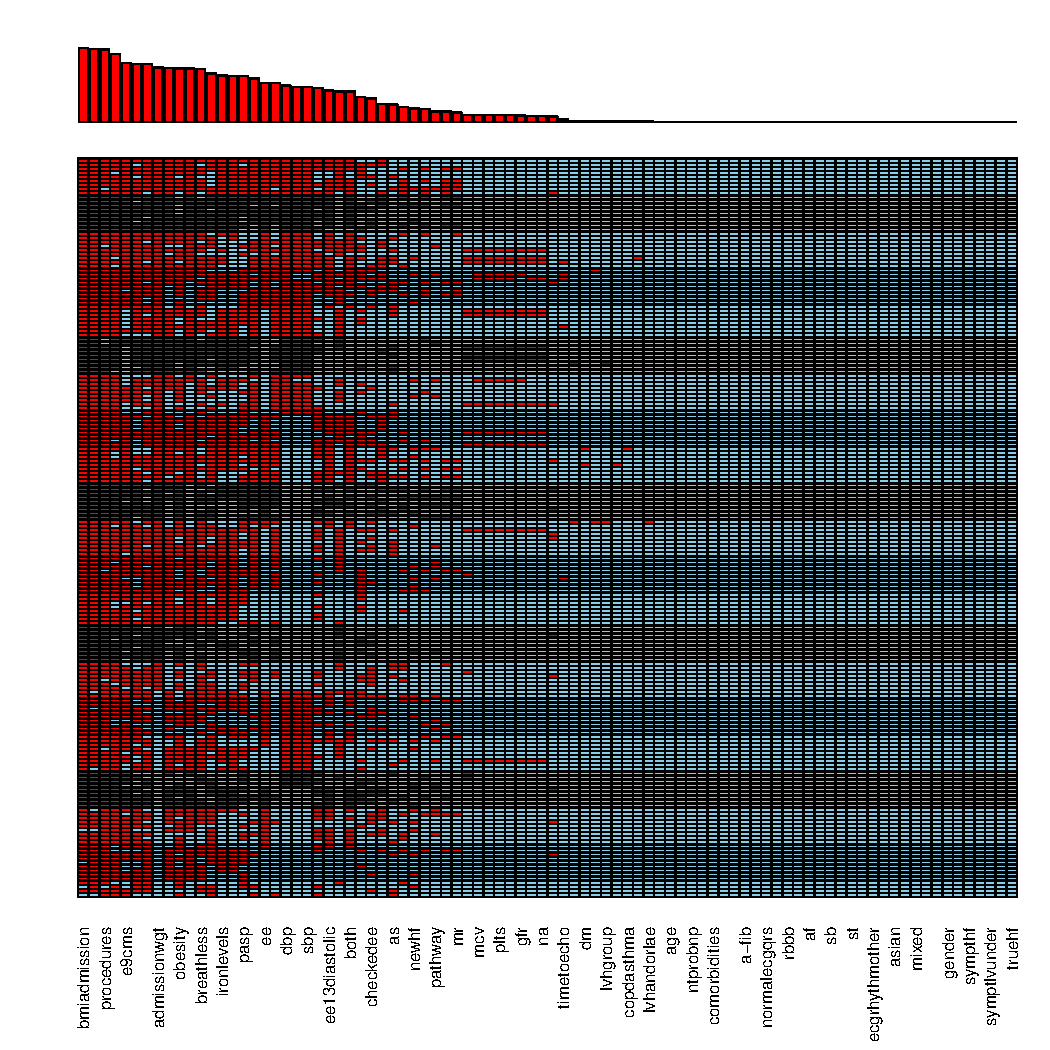
\includegraphics[width=1.1\textwidth]{doc/thesis/images/HFmrEF_miss_dist.pdf}
    \caption[Missing values in HFmrEF data set]{\textit{Missing values in HFmrEF data set. Top:  the amount of missing values in each variable sorted in ascending order. Bottom: plot of the combinations of missing (red) and non-missing (blue) values in the HFmrEF data set.}}
    \label{fig:HFmrEF_missing}
\end{figure}

\newpage

\begin{figure}[h!]
%\centering
%\hspace*{-1cm}\resizebox{1.1\textwidth}{!}{% Created by tikzDevice version 0.11 on 2018-05-09 15:09:57
% !TEX encoding = UTF-8 Unicode
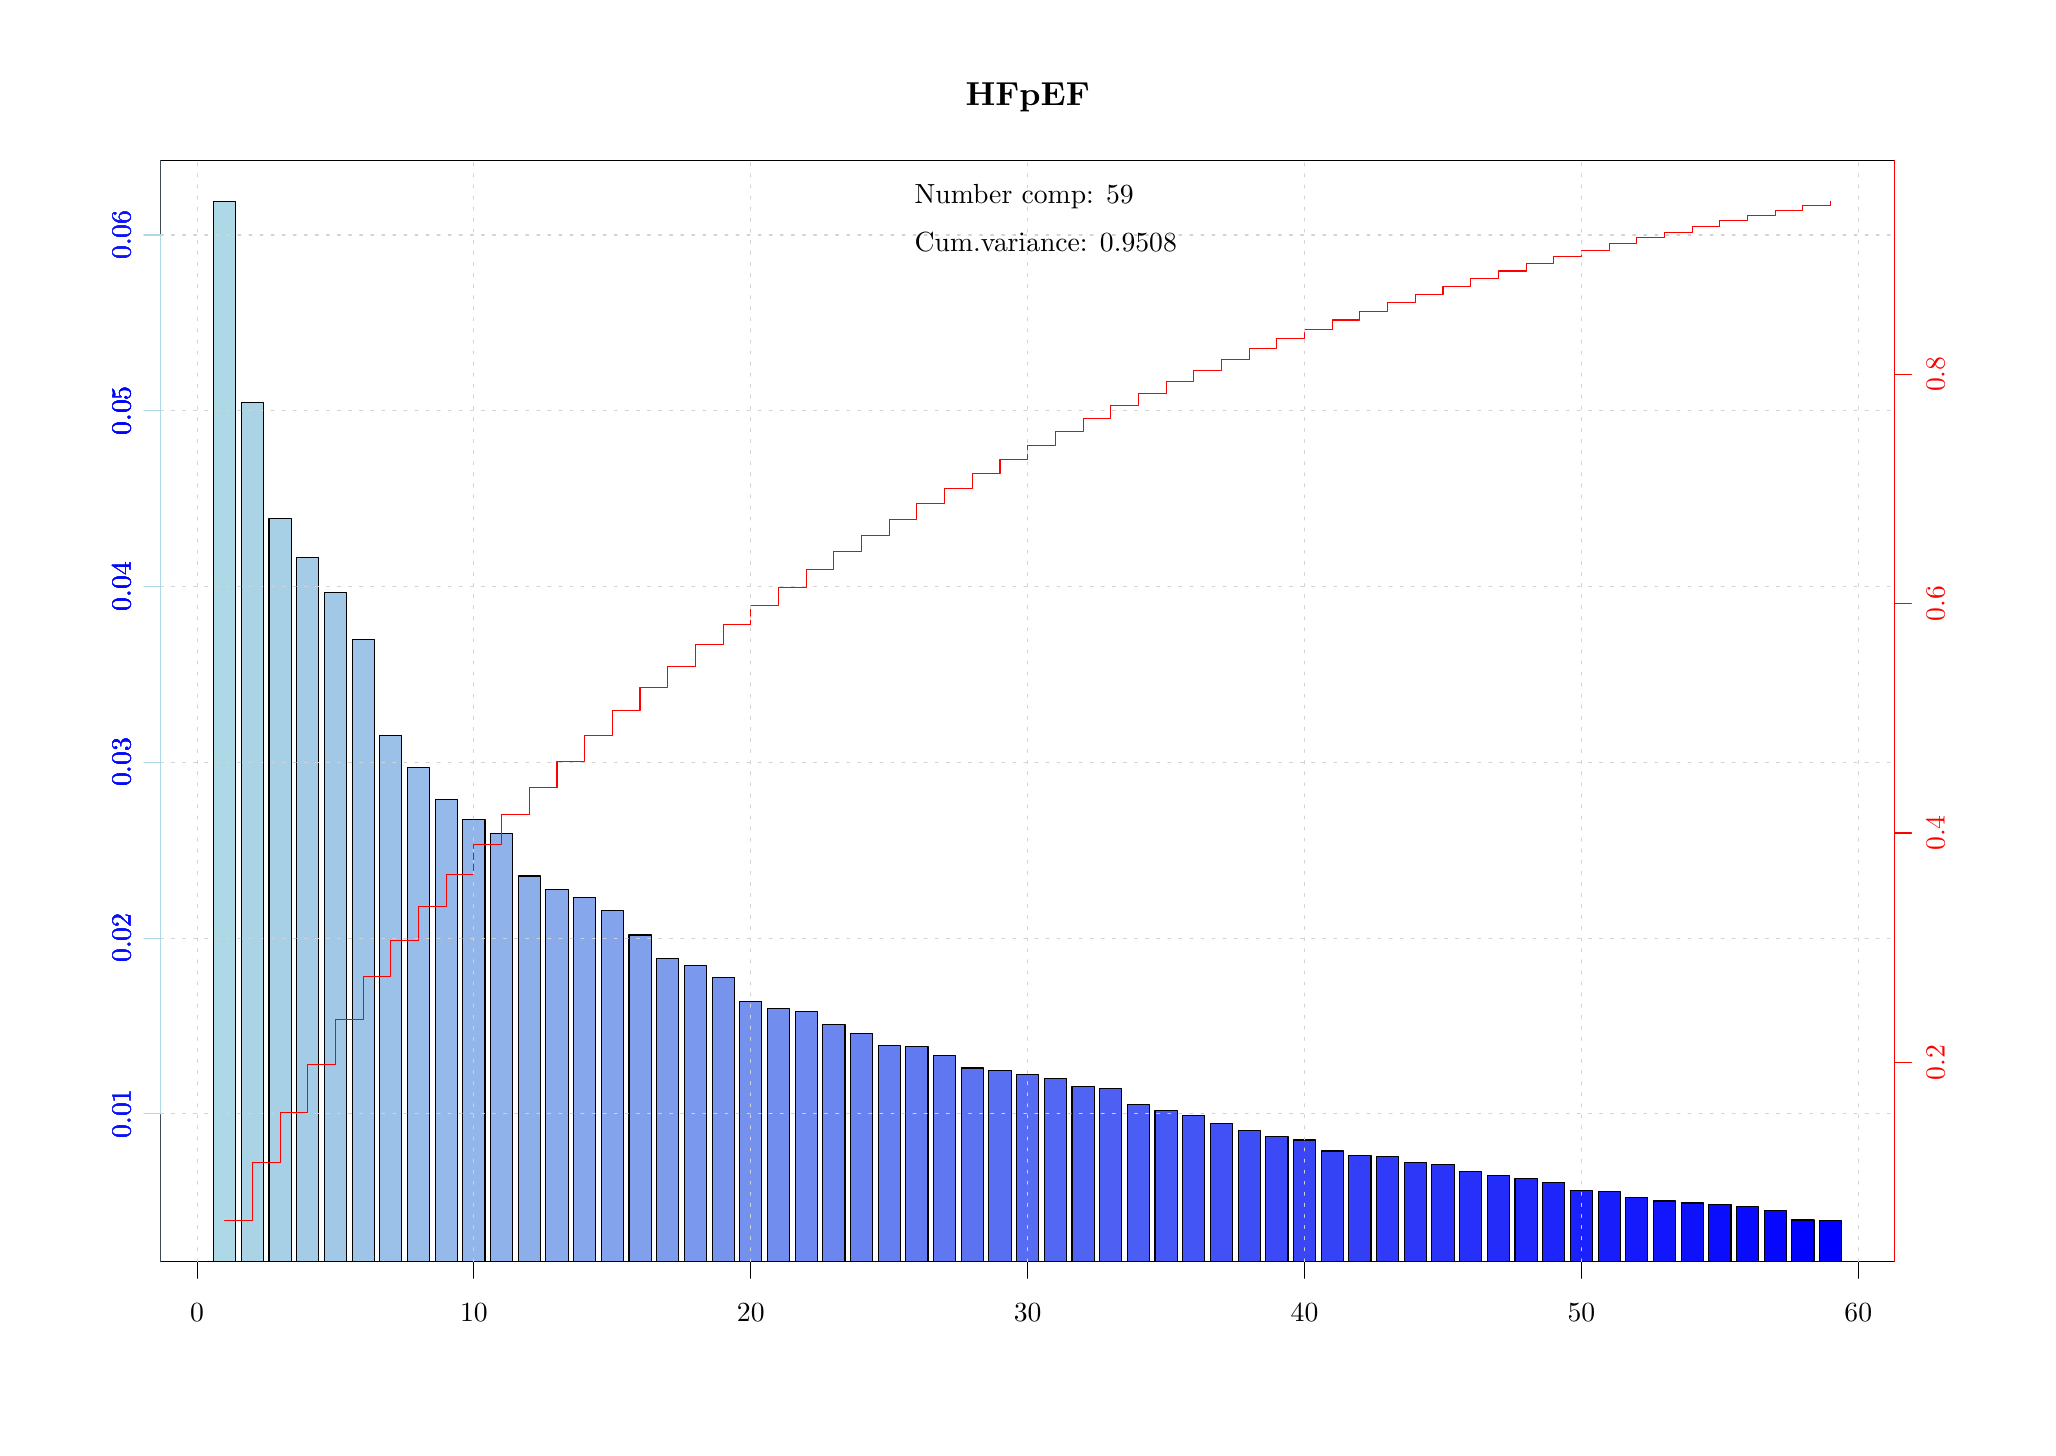
\begin{tikzpicture}[x=1pt,y=1pt]
\definecolor{fillColor}{RGB}{255,255,255}
\path[use as bounding box,fill=fillColor,fill opacity=0.00] (0,0) rectangle (722.70,505.89);
\begin{scope}
\path[clip] ( 48.00, 60.00) rectangle (674.70,457.89);
\definecolor{drawColor}{RGB}{0,0,0}
\definecolor{fillColor}{RGB}{173,216,230}

\path[draw=drawColor,line width= 0.4pt,line join=round,line cap=round,fill=fillColor] ( 67.21, 60.00) rectangle ( 75.21,443.15);
\definecolor{fillColor}{RGB}{170,212,230}

\path[draw=drawColor,line width= 0.4pt,line join=round,line cap=round,fill=fillColor] ( 77.21, 60.00) rectangle ( 85.22,370.44);
\definecolor{fillColor}{RGB}{167,208,230}

\path[draw=drawColor,line width= 0.4pt,line join=round,line cap=round,fill=fillColor] ( 87.22, 60.00) rectangle ( 95.22,328.47);
\definecolor{fillColor}{RGB}{164,204,231}

\path[draw=drawColor,line width= 0.4pt,line join=round,line cap=round,fill=fillColor] ( 97.22, 60.00) rectangle (105.23,314.38);
\definecolor{fillColor}{RGB}{161,201,231}

\path[draw=drawColor,line width= 0.4pt,line join=round,line cap=round,fill=fillColor] (107.23, 60.00) rectangle (115.23,301.74);
\definecolor{fillColor}{RGB}{158,197,232}

\path[draw=drawColor,line width= 0.4pt,line join=round,line cap=round,fill=fillColor] (117.23, 60.00) rectangle (125.24,284.82);
\definecolor{fillColor}{RGB}{155,193,232}

\path[draw=drawColor,line width= 0.4pt,line join=round,line cap=round,fill=fillColor] (127.24, 60.00) rectangle (135.24,250.18);
\definecolor{fillColor}{RGB}{152,189,233}

\path[draw=drawColor,line width= 0.4pt,line join=round,line cap=round,fill=fillColor] (137.24, 60.00) rectangle (145.25,238.52);
\definecolor{fillColor}{RGB}{149,186,233}

\path[draw=drawColor,line width= 0.4pt,line join=round,line cap=round,fill=fillColor] (147.25, 60.00) rectangle (155.25,226.92);
\definecolor{fillColor}{RGB}{146,182,233}

\path[draw=drawColor,line width= 0.4pt,line join=round,line cap=round,fill=fillColor] (157.25, 60.00) rectangle (165.26,219.61);
\definecolor{fillColor}{RGB}{143,178,234}

\path[draw=drawColor,line width= 0.4pt,line join=round,line cap=round,fill=fillColor] (167.26, 60.00) rectangle (175.26,214.78);
\definecolor{fillColor}{RGB}{140,175,234}

\path[draw=drawColor,line width= 0.4pt,line join=round,line cap=round,fill=fillColor] (177.26, 60.00) rectangle (185.27,199.34);
\definecolor{fillColor}{RGB}{137,171,235}

\path[draw=drawColor,line width= 0.4pt,line join=round,line cap=round,fill=fillColor] (187.27, 60.00) rectangle (195.27,194.32);
\definecolor{fillColor}{RGB}{134,167,235}

\path[draw=drawColor,line width= 0.4pt,line join=round,line cap=round,fill=fillColor] (197.27, 60.00) rectangle (205.28,191.69);
\definecolor{fillColor}{RGB}{131,163,236}

\path[draw=drawColor,line width= 0.4pt,line join=round,line cap=round,fill=fillColor] (207.28, 60.00) rectangle (215.28,186.94);
\definecolor{fillColor}{RGB}{128,160,236}

\path[draw=drawColor,line width= 0.4pt,line join=round,line cap=round,fill=fillColor] (217.28, 60.00) rectangle (225.28,178.03);
\definecolor{fillColor}{RGB}{125,156,236}

\path[draw=drawColor,line width= 0.4pt,line join=round,line cap=round,fill=fillColor] (227.29, 60.00) rectangle (235.29,169.60);
\definecolor{fillColor}{RGB}{122,152,237}

\path[draw=drawColor,line width= 0.4pt,line join=round,line cap=round,fill=fillColor] (237.29, 60.00) rectangle (245.29,166.92);
\definecolor{fillColor}{RGB}{119,148,237}

\path[draw=drawColor,line width= 0.4pt,line join=round,line cap=round,fill=fillColor] (247.30, 60.00) rectangle (255.30,162.63);
\definecolor{fillColor}{RGB}{116,145,238}

\path[draw=drawColor,line width= 0.4pt,line join=round,line cap=round,fill=fillColor] (257.30, 60.00) rectangle (265.30,154.09);
\definecolor{fillColor}{RGB}{113,141,238}

\path[draw=drawColor,line width= 0.4pt,line join=round,line cap=round,fill=fillColor] (267.30, 60.00) rectangle (275.31,151.41);
\definecolor{fillColor}{RGB}{110,137,239}

\path[draw=drawColor,line width= 0.4pt,line join=round,line cap=round,fill=fillColor] (277.31, 60.00) rectangle (285.31,150.50);
\definecolor{fillColor}{RGB}{107,134,239}

\path[draw=drawColor,line width= 0.4pt,line join=round,line cap=round,fill=fillColor] (287.31, 60.00) rectangle (295.32,145.67);
\definecolor{fillColor}{RGB}{104,130,239}

\path[draw=drawColor,line width= 0.4pt,line join=round,line cap=round,fill=fillColor] (297.32, 60.00) rectangle (305.32,142.52);
\definecolor{fillColor}{RGB}{101,126,240}

\path[draw=drawColor,line width= 0.4pt,line join=round,line cap=round,fill=fillColor] (307.32, 60.00) rectangle (315.33,138.07);
\definecolor{fillColor}{RGB}{98,122,240}

\path[draw=drawColor,line width= 0.4pt,line join=round,line cap=round,fill=fillColor] (317.33, 60.00) rectangle (325.33,137.58);
\definecolor{fillColor}{RGB}{95,119,241}

\path[draw=drawColor,line width= 0.4pt,line join=round,line cap=round,fill=fillColor] (327.33, 60.00) rectangle (335.34,134.45);
\definecolor{fillColor}{RGB}{92,115,241}

\path[draw=drawColor,line width= 0.4pt,line join=round,line cap=round,fill=fillColor] (337.34, 60.00) rectangle (345.34,129.97);
\definecolor{fillColor}{RGB}{89,111,242}

\path[draw=drawColor,line width= 0.4pt,line join=round,line cap=round,fill=fillColor] (347.34, 60.00) rectangle (355.35,128.91);
\definecolor{fillColor}{RGB}{86,108,242}

\path[draw=drawColor,line width= 0.4pt,line join=round,line cap=round,fill=fillColor] (357.35, 60.00) rectangle (365.35,127.68);
\definecolor{fillColor}{RGB}{83,104,242}

\path[draw=drawColor,line width= 0.4pt,line join=round,line cap=round,fill=fillColor] (367.35, 60.00) rectangle (375.36,126.21);
\definecolor{fillColor}{RGB}{80,100,243}

\path[draw=drawColor,line width= 0.4pt,line join=round,line cap=round,fill=fillColor] (377.36, 60.00) rectangle (385.36,123.34);
\definecolor{fillColor}{RGB}{77,96,243}

\path[draw=drawColor,line width= 0.4pt,line join=round,line cap=round,fill=fillColor] (387.36, 60.00) rectangle (395.37,122.47);
\definecolor{fillColor}{RGB}{74,93,244}

\path[draw=drawColor,line width= 0.4pt,line join=round,line cap=round,fill=fillColor] (397.37, 60.00) rectangle (405.37,116.77);
\definecolor{fillColor}{RGB}{71,89,244}

\path[draw=drawColor,line width= 0.4pt,line join=round,line cap=round,fill=fillColor] (407.37, 60.00) rectangle (415.38,114.47);
\definecolor{fillColor}{RGB}{68,85,245}

\path[draw=drawColor,line width= 0.4pt,line join=round,line cap=round,fill=fillColor] (417.38, 60.00) rectangle (425.38,112.87);
\definecolor{fillColor}{RGB}{65,81,245}

\path[draw=drawColor,line width= 0.4pt,line join=round,line cap=round,fill=fillColor] (427.38, 60.00) rectangle (435.39,109.91);
\definecolor{fillColor}{RGB}{62,78,245}

\path[draw=drawColor,line width= 0.4pt,line join=round,line cap=round,fill=fillColor] (437.39, 60.00) rectangle (445.39,107.53);
\definecolor{fillColor}{RGB}{59,74,246}

\path[draw=drawColor,line width= 0.4pt,line join=round,line cap=round,fill=fillColor] (447.39, 60.00) rectangle (455.40,105.12);
\definecolor{fillColor}{RGB}{56,70,246}

\path[draw=drawColor,line width= 0.4pt,line join=round,line cap=round,fill=fillColor] (457.40, 60.00) rectangle (465.40,103.94);
\definecolor{fillColor}{RGB}{53,67,247}

\path[draw=drawColor,line width= 0.4pt,line join=round,line cap=round,fill=fillColor] (467.40, 60.00) rectangle (475.40, 99.96);
\definecolor{fillColor}{RGB}{50,63,247}

\path[draw=drawColor,line width= 0.4pt,line join=round,line cap=round,fill=fillColor] (477.41, 60.00) rectangle (485.41, 98.48);
\definecolor{fillColor}{RGB}{47,59,248}

\path[draw=drawColor,line width= 0.4pt,line join=round,line cap=round,fill=fillColor] (487.41, 60.00) rectangle (495.41, 97.84);
\definecolor{fillColor}{RGB}{44,55,248}

\path[draw=drawColor,line width= 0.4pt,line join=round,line cap=round,fill=fillColor] (497.42, 60.00) rectangle (505.42, 95.79);
\definecolor{fillColor}{RGB}{41,52,248}

\path[draw=drawColor,line width= 0.4pt,line join=round,line cap=round,fill=fillColor] (507.42, 60.00) rectangle (515.42, 95.01);
\definecolor{fillColor}{RGB}{38,48,249}

\path[draw=drawColor,line width= 0.4pt,line join=round,line cap=round,fill=fillColor] (517.42, 60.00) rectangle (525.43, 92.41);
\definecolor{fillColor}{RGB}{35,44,249}

\path[draw=drawColor,line width= 0.4pt,line join=round,line cap=round,fill=fillColor] (527.43, 60.00) rectangle (535.43, 91.07);
\definecolor{fillColor}{RGB}{32,40,250}

\path[draw=drawColor,line width= 0.4pt,line join=round,line cap=round,fill=fillColor] (537.43, 60.00) rectangle (545.44, 89.97);
\definecolor{fillColor}{RGB}{29,37,250}

\path[draw=drawColor,line width= 0.4pt,line join=round,line cap=round,fill=fillColor] (547.44, 60.00) rectangle (555.44, 88.72);
\definecolor{fillColor}{RGB}{26,33,251}

\path[draw=drawColor,line width= 0.4pt,line join=round,line cap=round,fill=fillColor] (557.44, 60.00) rectangle (565.45, 85.69);
\definecolor{fillColor}{RGB}{23,29,251}

\path[draw=drawColor,line width= 0.4pt,line join=round,line cap=round,fill=fillColor] (567.45, 60.00) rectangle (575.45, 85.39);
\definecolor{fillColor}{RGB}{20,26,251}

\path[draw=drawColor,line width= 0.4pt,line join=round,line cap=round,fill=fillColor] (577.45, 60.00) rectangle (585.46, 83.21);
\definecolor{fillColor}{RGB}{17,22,252}

\path[draw=drawColor,line width= 0.4pt,line join=round,line cap=round,fill=fillColor] (587.46, 60.00) rectangle (595.46, 81.89);
\definecolor{fillColor}{RGB}{14,18,252}

\path[draw=drawColor,line width= 0.4pt,line join=round,line cap=round,fill=fillColor] (597.46, 60.00) rectangle (605.47, 81.17);
\definecolor{fillColor}{RGB}{11,14,253}

\path[draw=drawColor,line width= 0.4pt,line join=round,line cap=round,fill=fillColor] (607.47, 60.00) rectangle (615.47, 80.50);
\definecolor{fillColor}{RGB}{8,11,253}

\path[draw=drawColor,line width= 0.4pt,line join=round,line cap=round,fill=fillColor] (617.47, 60.00) rectangle (625.48, 79.78);
\definecolor{fillColor}{RGB}{5,7,254}

\path[draw=drawColor,line width= 0.4pt,line join=round,line cap=round,fill=fillColor] (627.48, 60.00) rectangle (635.48, 78.63);
\definecolor{fillColor}{RGB}{2,3,254}

\path[draw=drawColor,line width= 0.4pt,line join=round,line cap=round,fill=fillColor] (637.48, 60.00) rectangle (645.49, 75.04);
\definecolor{fillColor}{RGB}{0,0,255}

\path[draw=drawColor,line width= 0.4pt,line join=round,line cap=round,fill=fillColor] (647.49, 60.00) rectangle (655.49, 74.74);
\end{scope}
\begin{scope}
\path[clip] (  0.00,  0.00) rectangle (722.70,505.89);
\definecolor{drawColor}{RGB}{0,0,0}

\node[text=drawColor,anchor=base,inner sep=0pt, outer sep=0pt, scale=  1.20] at (361.35,477.75) {\bfseries HFpEF};
\end{scope}
\begin{scope}
\path[clip] (  0.00,  0.00) rectangle (722.70,505.89);
\definecolor{drawColor}{RGB}{0,0,0}

\path[draw=drawColor,line width= 0.4pt,line join=round,line cap=round] ( 48.00, 60.00) --
	(674.70, 60.00) --
	(674.70,457.89) --
	( 48.00,457.89) --
	( 48.00, 60.00);

\path[draw=drawColor,line width= 0.4pt,line join=round,line cap=round] ( 61.21, 60.00) -- (661.49, 60.00);

\path[draw=drawColor,line width= 0.4pt,line join=round,line cap=round] ( 61.21, 60.00) -- ( 61.21, 54.00);

\path[draw=drawColor,line width= 0.4pt,line join=round,line cap=round] (161.25, 60.00) -- (161.25, 54.00);

\path[draw=drawColor,line width= 0.4pt,line join=round,line cap=round] (261.30, 60.00) -- (261.30, 54.00);

\path[draw=drawColor,line width= 0.4pt,line join=round,line cap=round] (361.35, 60.00) -- (361.35, 54.00);

\path[draw=drawColor,line width= 0.4pt,line join=round,line cap=round] (461.40, 60.00) -- (461.40, 54.00);

\path[draw=drawColor,line width= 0.4pt,line join=round,line cap=round] (561.45, 60.00) -- (561.45, 54.00);

\path[draw=drawColor,line width= 0.4pt,line join=round,line cap=round] (661.49, 60.00) -- (661.49, 54.00);

\node[text=drawColor,anchor=base,inner sep=0pt, outer sep=0pt, scale=  1.00] at ( 61.21, 38.40) {0};

\node[text=drawColor,anchor=base,inner sep=0pt, outer sep=0pt, scale=  1.00] at (161.25, 38.40) {10};

\node[text=drawColor,anchor=base,inner sep=0pt, outer sep=0pt, scale=  1.00] at (261.30, 38.40) {20};

\node[text=drawColor,anchor=base,inner sep=0pt, outer sep=0pt, scale=  1.00] at (361.35, 38.40) {30};

\node[text=drawColor,anchor=base,inner sep=0pt, outer sep=0pt, scale=  1.00] at (461.40, 38.40) {40};

\node[text=drawColor,anchor=base,inner sep=0pt, outer sep=0pt, scale=  1.00] at (561.45, 38.40) {50};

\node[text=drawColor,anchor=base,inner sep=0pt, outer sep=0pt, scale=  1.00] at (661.49, 38.40) {60};
\definecolor{drawColor}{RGB}{173,216,230}

\path[draw=drawColor,line width= 0.4pt,line join=round,line cap=round] ( 48.00,113.39) -- ( 48.00,430.96);

\path[draw=drawColor,line width= 0.4pt,line join=round,line cap=round] ( 48.00,113.39) -- ( 42.00,113.39);

\path[draw=drawColor,line width= 0.4pt,line join=round,line cap=round] ( 48.00,176.90) -- ( 42.00,176.90);

\path[draw=drawColor,line width= 0.4pt,line join=round,line cap=round] ( 48.00,240.42) -- ( 42.00,240.42);

\path[draw=drawColor,line width= 0.4pt,line join=round,line cap=round] ( 48.00,303.93) -- ( 42.00,303.93);

\path[draw=drawColor,line width= 0.4pt,line join=round,line cap=round] ( 48.00,367.44) -- ( 42.00,367.44);

\path[draw=drawColor,line width= 0.4pt,line join=round,line cap=round] ( 48.00,430.96) -- ( 42.00,430.96);

\node[text=drawColor,rotate= 90.00,anchor=base,inner sep=0pt, outer sep=0pt, scale=  1.00] at ( 37.20,113.39) {0.01};
\definecolor{drawColor}{RGB}{170,212,230}

\node[text=drawColor,rotate= 90.00,anchor=base,inner sep=0pt, outer sep=0pt, scale=  1.00] at ( 37.20,176.90) {0.02};
\definecolor{drawColor}{RGB}{167,208,230}

\node[text=drawColor,rotate= 90.00,anchor=base,inner sep=0pt, outer sep=0pt, scale=  1.00] at ( 37.20,240.42) {0.03};
\definecolor{drawColor}{RGB}{164,204,231}

\node[text=drawColor,rotate= 90.00,anchor=base,inner sep=0pt, outer sep=0pt, scale=  1.00] at ( 37.20,303.93) {0.04};
\definecolor{drawColor}{RGB}{161,201,231}

\node[text=drawColor,rotate= 90.00,anchor=base,inner sep=0pt, outer sep=0pt, scale=  1.00] at ( 37.20,367.44) {0.05};
\definecolor{drawColor}{RGB}{158,197,232}

\node[text=drawColor,rotate= 90.00,anchor=base,inner sep=0pt, outer sep=0pt, scale=  1.00] at ( 37.20,430.96) {0.06};
\definecolor{drawColor}{RGB}{155,193,232}

\node[text=drawColor,rotate= 90.00,anchor=base,inner sep=0pt, outer sep=0pt, scale=  1.00] at ( 37.20,113.39) {0.01};
\definecolor{drawColor}{RGB}{152,189,233}

\node[text=drawColor,rotate= 90.00,anchor=base,inner sep=0pt, outer sep=0pt, scale=  1.00] at ( 37.20,176.90) {0.02};
\definecolor{drawColor}{RGB}{149,186,233}

\node[text=drawColor,rotate= 90.00,anchor=base,inner sep=0pt, outer sep=0pt, scale=  1.00] at ( 37.20,240.42) {0.03};
\definecolor{drawColor}{RGB}{146,182,233}

\node[text=drawColor,rotate= 90.00,anchor=base,inner sep=0pt, outer sep=0pt, scale=  1.00] at ( 37.20,303.93) {0.04};
\definecolor{drawColor}{RGB}{143,178,234}

\node[text=drawColor,rotate= 90.00,anchor=base,inner sep=0pt, outer sep=0pt, scale=  1.00] at ( 37.20,367.44) {0.05};
\definecolor{drawColor}{RGB}{140,175,234}

\node[text=drawColor,rotate= 90.00,anchor=base,inner sep=0pt, outer sep=0pt, scale=  1.00] at ( 37.20,430.96) {0.06};
\definecolor{drawColor}{RGB}{137,171,235}

\node[text=drawColor,rotate= 90.00,anchor=base,inner sep=0pt, outer sep=0pt, scale=  1.00] at ( 37.20,113.39) {0.01};
\definecolor{drawColor}{RGB}{134,167,235}

\node[text=drawColor,rotate= 90.00,anchor=base,inner sep=0pt, outer sep=0pt, scale=  1.00] at ( 37.20,176.90) {0.02};
\definecolor{drawColor}{RGB}{131,163,236}

\node[text=drawColor,rotate= 90.00,anchor=base,inner sep=0pt, outer sep=0pt, scale=  1.00] at ( 37.20,240.42) {0.03};
\definecolor{drawColor}{RGB}{128,160,236}

\node[text=drawColor,rotate= 90.00,anchor=base,inner sep=0pt, outer sep=0pt, scale=  1.00] at ( 37.20,303.93) {0.04};
\definecolor{drawColor}{RGB}{125,156,236}

\node[text=drawColor,rotate= 90.00,anchor=base,inner sep=0pt, outer sep=0pt, scale=  1.00] at ( 37.20,367.44) {0.05};
\definecolor{drawColor}{RGB}{122,152,237}

\node[text=drawColor,rotate= 90.00,anchor=base,inner sep=0pt, outer sep=0pt, scale=  1.00] at ( 37.20,430.96) {0.06};
\definecolor{drawColor}{RGB}{119,148,237}

\node[text=drawColor,rotate= 90.00,anchor=base,inner sep=0pt, outer sep=0pt, scale=  1.00] at ( 37.20,113.39) {0.01};
\definecolor{drawColor}{RGB}{116,145,238}

\node[text=drawColor,rotate= 90.00,anchor=base,inner sep=0pt, outer sep=0pt, scale=  1.00] at ( 37.20,176.90) {0.02};
\definecolor{drawColor}{RGB}{113,141,238}

\node[text=drawColor,rotate= 90.00,anchor=base,inner sep=0pt, outer sep=0pt, scale=  1.00] at ( 37.20,240.42) {0.03};
\definecolor{drawColor}{RGB}{110,137,239}

\node[text=drawColor,rotate= 90.00,anchor=base,inner sep=0pt, outer sep=0pt, scale=  1.00] at ( 37.20,303.93) {0.04};
\definecolor{drawColor}{RGB}{107,134,239}

\node[text=drawColor,rotate= 90.00,anchor=base,inner sep=0pt, outer sep=0pt, scale=  1.00] at ( 37.20,367.44) {0.05};
\definecolor{drawColor}{RGB}{104,130,239}

\node[text=drawColor,rotate= 90.00,anchor=base,inner sep=0pt, outer sep=0pt, scale=  1.00] at ( 37.20,430.96) {0.06};
\definecolor{drawColor}{RGB}{101,126,240}

\node[text=drawColor,rotate= 90.00,anchor=base,inner sep=0pt, outer sep=0pt, scale=  1.00] at ( 37.20,113.39) {0.01};
\definecolor{drawColor}{RGB}{98,122,240}

\node[text=drawColor,rotate= 90.00,anchor=base,inner sep=0pt, outer sep=0pt, scale=  1.00] at ( 37.20,176.90) {0.02};
\definecolor{drawColor}{RGB}{95,119,241}

\node[text=drawColor,rotate= 90.00,anchor=base,inner sep=0pt, outer sep=0pt, scale=  1.00] at ( 37.20,240.42) {0.03};
\definecolor{drawColor}{RGB}{92,115,241}

\node[text=drawColor,rotate= 90.00,anchor=base,inner sep=0pt, outer sep=0pt, scale=  1.00] at ( 37.20,303.93) {0.04};
\definecolor{drawColor}{RGB}{89,111,242}

\node[text=drawColor,rotate= 90.00,anchor=base,inner sep=0pt, outer sep=0pt, scale=  1.00] at ( 37.20,367.44) {0.05};
\definecolor{drawColor}{RGB}{86,108,242}

\node[text=drawColor,rotate= 90.00,anchor=base,inner sep=0pt, outer sep=0pt, scale=  1.00] at ( 37.20,430.96) {0.06};
\definecolor{drawColor}{RGB}{83,104,242}

\node[text=drawColor,rotate= 90.00,anchor=base,inner sep=0pt, outer sep=0pt, scale=  1.00] at ( 37.20,113.39) {0.01};
\definecolor{drawColor}{RGB}{80,100,243}

\node[text=drawColor,rotate= 90.00,anchor=base,inner sep=0pt, outer sep=0pt, scale=  1.00] at ( 37.20,176.90) {0.02};
\definecolor{drawColor}{RGB}{77,96,243}

\node[text=drawColor,rotate= 90.00,anchor=base,inner sep=0pt, outer sep=0pt, scale=  1.00] at ( 37.20,240.42) {0.03};
\definecolor{drawColor}{RGB}{74,93,244}

\node[text=drawColor,rotate= 90.00,anchor=base,inner sep=0pt, outer sep=0pt, scale=  1.00] at ( 37.20,303.93) {0.04};
\definecolor{drawColor}{RGB}{71,89,244}

\node[text=drawColor,rotate= 90.00,anchor=base,inner sep=0pt, outer sep=0pt, scale=  1.00] at ( 37.20,367.44) {0.05};
\definecolor{drawColor}{RGB}{68,85,245}

\node[text=drawColor,rotate= 90.00,anchor=base,inner sep=0pt, outer sep=0pt, scale=  1.00] at ( 37.20,430.96) {0.06};
\definecolor{drawColor}{RGB}{65,81,245}

\node[text=drawColor,rotate= 90.00,anchor=base,inner sep=0pt, outer sep=0pt, scale=  1.00] at ( 37.20,113.39) {0.01};
\definecolor{drawColor}{RGB}{62,78,245}

\node[text=drawColor,rotate= 90.00,anchor=base,inner sep=0pt, outer sep=0pt, scale=  1.00] at ( 37.20,176.90) {0.02};
\definecolor{drawColor}{RGB}{59,74,246}

\node[text=drawColor,rotate= 90.00,anchor=base,inner sep=0pt, outer sep=0pt, scale=  1.00] at ( 37.20,240.42) {0.03};
\definecolor{drawColor}{RGB}{56,70,246}

\node[text=drawColor,rotate= 90.00,anchor=base,inner sep=0pt, outer sep=0pt, scale=  1.00] at ( 37.20,303.93) {0.04};
\definecolor{drawColor}{RGB}{53,67,247}

\node[text=drawColor,rotate= 90.00,anchor=base,inner sep=0pt, outer sep=0pt, scale=  1.00] at ( 37.20,367.44) {0.05};
\definecolor{drawColor}{RGB}{50,63,247}

\node[text=drawColor,rotate= 90.00,anchor=base,inner sep=0pt, outer sep=0pt, scale=  1.00] at ( 37.20,430.96) {0.06};
\definecolor{drawColor}{RGB}{47,59,248}

\node[text=drawColor,rotate= 90.00,anchor=base,inner sep=0pt, outer sep=0pt, scale=  1.00] at ( 37.20,113.39) {0.01};
\definecolor{drawColor}{RGB}{44,55,248}

\node[text=drawColor,rotate= 90.00,anchor=base,inner sep=0pt, outer sep=0pt, scale=  1.00] at ( 37.20,176.90) {0.02};
\definecolor{drawColor}{RGB}{41,52,248}

\node[text=drawColor,rotate= 90.00,anchor=base,inner sep=0pt, outer sep=0pt, scale=  1.00] at ( 37.20,240.42) {0.03};
\definecolor{drawColor}{RGB}{38,48,249}

\node[text=drawColor,rotate= 90.00,anchor=base,inner sep=0pt, outer sep=0pt, scale=  1.00] at ( 37.20,303.93) {0.04};
\definecolor{drawColor}{RGB}{35,44,249}

\node[text=drawColor,rotate= 90.00,anchor=base,inner sep=0pt, outer sep=0pt, scale=  1.00] at ( 37.20,367.44) {0.05};
\definecolor{drawColor}{RGB}{32,40,250}

\node[text=drawColor,rotate= 90.00,anchor=base,inner sep=0pt, outer sep=0pt, scale=  1.00] at ( 37.20,430.96) {0.06};
\definecolor{drawColor}{RGB}{29,37,250}

\node[text=drawColor,rotate= 90.00,anchor=base,inner sep=0pt, outer sep=0pt, scale=  1.00] at ( 37.20,113.39) {0.01};
\definecolor{drawColor}{RGB}{26,33,251}

\node[text=drawColor,rotate= 90.00,anchor=base,inner sep=0pt, outer sep=0pt, scale=  1.00] at ( 37.20,176.90) {0.02};
\definecolor{drawColor}{RGB}{23,29,251}

\node[text=drawColor,rotate= 90.00,anchor=base,inner sep=0pt, outer sep=0pt, scale=  1.00] at ( 37.20,240.42) {0.03};
\definecolor{drawColor}{RGB}{20,26,251}

\node[text=drawColor,rotate= 90.00,anchor=base,inner sep=0pt, outer sep=0pt, scale=  1.00] at ( 37.20,303.93) {0.04};
\definecolor{drawColor}{RGB}{17,22,252}

\node[text=drawColor,rotate= 90.00,anchor=base,inner sep=0pt, outer sep=0pt, scale=  1.00] at ( 37.20,367.44) {0.05};
\definecolor{drawColor}{RGB}{14,18,252}

\node[text=drawColor,rotate= 90.00,anchor=base,inner sep=0pt, outer sep=0pt, scale=  1.00] at ( 37.20,430.96) {0.06};
\definecolor{drawColor}{RGB}{11,14,253}

\node[text=drawColor,rotate= 90.00,anchor=base,inner sep=0pt, outer sep=0pt, scale=  1.00] at ( 37.20,113.39) {0.01};
\definecolor{drawColor}{RGB}{8,11,253}

\node[text=drawColor,rotate= 90.00,anchor=base,inner sep=0pt, outer sep=0pt, scale=  1.00] at ( 37.20,176.90) {0.02};
\definecolor{drawColor}{RGB}{5,7,254}

\node[text=drawColor,rotate= 90.00,anchor=base,inner sep=0pt, outer sep=0pt, scale=  1.00] at ( 37.20,240.42) {0.03};
\definecolor{drawColor}{RGB}{2,3,254}

\node[text=drawColor,rotate= 90.00,anchor=base,inner sep=0pt, outer sep=0pt, scale=  1.00] at ( 37.20,303.93) {0.04};
\definecolor{drawColor}{RGB}{0,0,255}

\node[text=drawColor,rotate= 90.00,anchor=base,inner sep=0pt, outer sep=0pt, scale=  1.00] at ( 37.20,367.44) {0.05};
\end{scope}
\begin{scope}
\path[clip] ( 48.00, 60.00) rectangle (674.70,457.89);
\definecolor{drawColor}{RGB}{173,216,230}

\path[draw=drawColor,line width= 0.4pt,line join=round,line cap=round] ( 48.00, 60.00) -- ( 48.00,457.89);
\definecolor{drawColor}{RGB}{255,0,0}

\path[draw=drawColor,line width= 0.4pt,line join=round,line cap=round] ( 71.21, 74.74) --
	( 81.22, 74.74) --
	( 81.22, 95.66) --
	( 91.22, 95.66) --
	( 91.22,113.84) --
	(101.23,113.84) --
	(101.23,131.10) --
	(111.23,131.10) --
	(111.23,147.54) --
	(121.24,147.54) --
	(121.24,162.87) --
	(131.24,162.87) --
	(131.24,175.94) --
	(141.24,175.94) --
	(141.24,188.25) --
	(151.25,188.25) --
	(151.25,199.81) --
	(161.25,199.81) --
	(161.25,210.88) --
	(171.26,210.88) --
	(171.26,221.64) --
	(181.26,221.64) --
	(181.26,231.40) --
	(191.27,231.40) --
	(191.27,240.82) --
	(201.27,240.82) --
	(201.27,250.08) --
	(211.28,250.08) --
	(211.28,259.02) --
	(221.28,259.02) --
	(221.28,267.39) --
	(231.29,267.39) --
	(231.29,275.20) --
	(241.29,275.20) --
	(241.29,282.84) --
	(251.30,282.84) --
	(251.30,290.20) --
	(261.30,290.20) --
	(261.30,297.00) --
	(271.31,297.00) --
	(271.31,303.62) --
	(281.31,303.62) --
	(281.31,310.19) --
	(291.32,310.19) --
	(291.32,316.44) --
	(301.32,316.44) --
	(301.32,322.49) --
	(311.33,322.49) --
	(311.33,328.24) --
	(321.33,328.24) --
	(321.33,333.97) --
	(331.34,333.97) --
	(331.34,339.49) --
	(341.34,339.49) --
	(341.34,344.71) --
	(351.35,344.71) --
	(351.35,349.87) --
	(361.35,349.87) --
	(361.35,354.95) --
	(371.35,354.95) --
	(371.35,359.93) --
	(381.36,359.93) --
	(381.36,364.73) --
	(391.36,364.73) --
	(391.36,369.46) --
	(401.37,369.46) --
	(401.37,373.83) --
	(411.37,373.83) --
	(411.37,378.05) --
	(421.38,378.05) --
	(421.38,382.16) --
	(431.38,382.16) --
	(431.38,386.07) --
	(441.39,386.07) --
	(441.39,389.84) --
	(451.39,389.84) --
	(451.39,393.44) --
	(461.40,393.44) --
	(461.40,396.97) --
	(471.40,396.97) --
	(471.40,400.24) --
	(481.41,400.24) --
	(481.41,403.41) --
	(491.41,403.41) --
	(491.41,406.54) --
	(501.42,406.54) --
	(501.42,409.54) --
	(511.42,409.54) --
	(511.42,412.48) --
	(521.43,412.48) --
	(521.43,415.26) --
	(531.43,415.26) --
	(531.43,417.95) --
	(541.44,417.95) --
	(541.44,420.56) --
	(551.44,420.56) --
	(551.44,423.10) --
	(561.45,423.10) --
	(561.45,425.44) --
	(571.45,425.44) --
	(571.45,427.75) --
	(581.46,427.75) --
	(581.46,429.93) --
	(591.46,429.93) --
	(591.46,432.02) --
	(601.46,432.02) --
	(601.46,434.06) --
	(611.47,434.06) --
	(611.47,436.06) --
	(621.47,436.06) --
	(621.47,438.01) --
	(631.48,438.01) --
	(631.48,439.89) --
	(641.48,439.89) --
	(641.48,441.53) --
	(651.49,441.53) --
	(651.49,443.15);
\end{scope}
\begin{scope}
\path[clip] (  0.00,  0.00) rectangle (722.70,505.89);
\definecolor{drawColor}{RGB}{255,0,0}

\path[draw=drawColor,line width= 0.4pt,line join=round,line cap=round] (674.70,131.97) -- (674.70,380.66);

\path[draw=drawColor,line width= 0.4pt,line join=round,line cap=round] (674.70,131.97) -- (680.70,131.97);

\path[draw=drawColor,line width= 0.4pt,line join=round,line cap=round] (674.70,214.87) -- (680.70,214.87);

\path[draw=drawColor,line width= 0.4pt,line join=round,line cap=round] (674.70,297.77) -- (680.70,297.77);

\path[draw=drawColor,line width= 0.4pt,line join=round,line cap=round] (674.70,380.66) -- (680.70,380.66);

\node[text=drawColor,rotate= 90.00,anchor=base,inner sep=0pt, outer sep=0pt, scale=  1.00] at (692.70,131.97) {0.2};

\node[text=drawColor,rotate= 90.00,anchor=base,inner sep=0pt, outer sep=0pt, scale=  1.00] at (692.70,214.87) {0.4};

\node[text=drawColor,rotate= 90.00,anchor=base,inner sep=0pt, outer sep=0pt, scale=  1.00] at (692.70,297.77) {0.6};

\node[text=drawColor,rotate= 90.00,anchor=base,inner sep=0pt, outer sep=0pt, scale=  1.00] at (692.70,380.66) {0.8};
\end{scope}
\begin{scope}
\path[clip] ( 48.00, 60.00) rectangle (674.70,457.89);
\definecolor{drawColor}{RGB}{255,0,0}

\path[draw=drawColor,line width= 0.4pt,line join=round,line cap=round] (674.70, 60.00) -- (674.70,457.89);
\definecolor{drawColor}{RGB}{211,211,211}

\path[draw=drawColor,line width= 0.4pt,dash pattern=on 1pt off 3pt ,line join=round,line cap=round] ( 61.21, 60.00) -- ( 61.21,457.89);

\path[draw=drawColor,line width= 0.4pt,dash pattern=on 1pt off 3pt ,line join=round,line cap=round] (161.25, 60.00) -- (161.25,457.89);

\path[draw=drawColor,line width= 0.4pt,dash pattern=on 1pt off 3pt ,line join=round,line cap=round] (261.30, 60.00) -- (261.30,457.89);

\path[draw=drawColor,line width= 0.4pt,dash pattern=on 1pt off 3pt ,line join=round,line cap=round] (361.35, 60.00) -- (361.35,457.89);

\path[draw=drawColor,line width= 0.4pt,dash pattern=on 1pt off 3pt ,line join=round,line cap=round] (461.40, 60.00) -- (461.40,457.89);

\path[draw=drawColor,line width= 0.4pt,dash pattern=on 1pt off 3pt ,line join=round,line cap=round] (561.45, 60.00) -- (561.45,457.89);

\path[draw=drawColor,line width= 0.4pt,dash pattern=on 1pt off 3pt ,line join=round,line cap=round] (661.49, 60.00) -- (661.49,457.89);

\path[draw=drawColor,line width= 0.4pt,dash pattern=on 1pt off 3pt ,line join=round,line cap=round] ( 48.00,113.39) -- (674.70,113.39);

\path[draw=drawColor,line width= 0.4pt,dash pattern=on 1pt off 3pt ,line join=round,line cap=round] ( 48.00,176.90) -- (674.70,176.90);

\path[draw=drawColor,line width= 0.4pt,dash pattern=on 1pt off 3pt ,line join=round,line cap=round] ( 48.00,240.42) -- (674.70,240.42);

\path[draw=drawColor,line width= 0.4pt,dash pattern=on 1pt off 3pt ,line join=round,line cap=round] ( 48.00,303.93) -- (674.70,303.93);

\path[draw=drawColor,line width= 0.4pt,dash pattern=on 1pt off 3pt ,line join=round,line cap=round] ( 48.00,367.44) -- (674.70,367.44);

\path[draw=drawColor,line width= 0.4pt,dash pattern=on 1pt off 3pt ,line join=round,line cap=round] ( 48.00,430.96) -- (674.70,430.96);
\definecolor{drawColor}{RGB}{0,0,0}

\node[text=drawColor,anchor=base west,inner sep=0pt, outer sep=0pt, scale=  1.00] at (320.51,442.37) {Number comp: 59};

\node[text=drawColor,anchor=base west,inner sep=0pt, outer sep=0pt, scale=  1.00] at (320.51,425) {Cum.variance: 0.9508};
\end{scope}
\end{tikzpicture}
}
%\caption{\textit{Explained variance (blue) and cumulative explained variance (red) for $n = 59$ principal components in HFpEF data set.}}
%\resizebox{0.65\textwidth}{!}{\LARGE% Created by tikzDevice version 0.11 on 2018-05-09 14:27:11
% !TEX encoding = UTF-8 Unicode
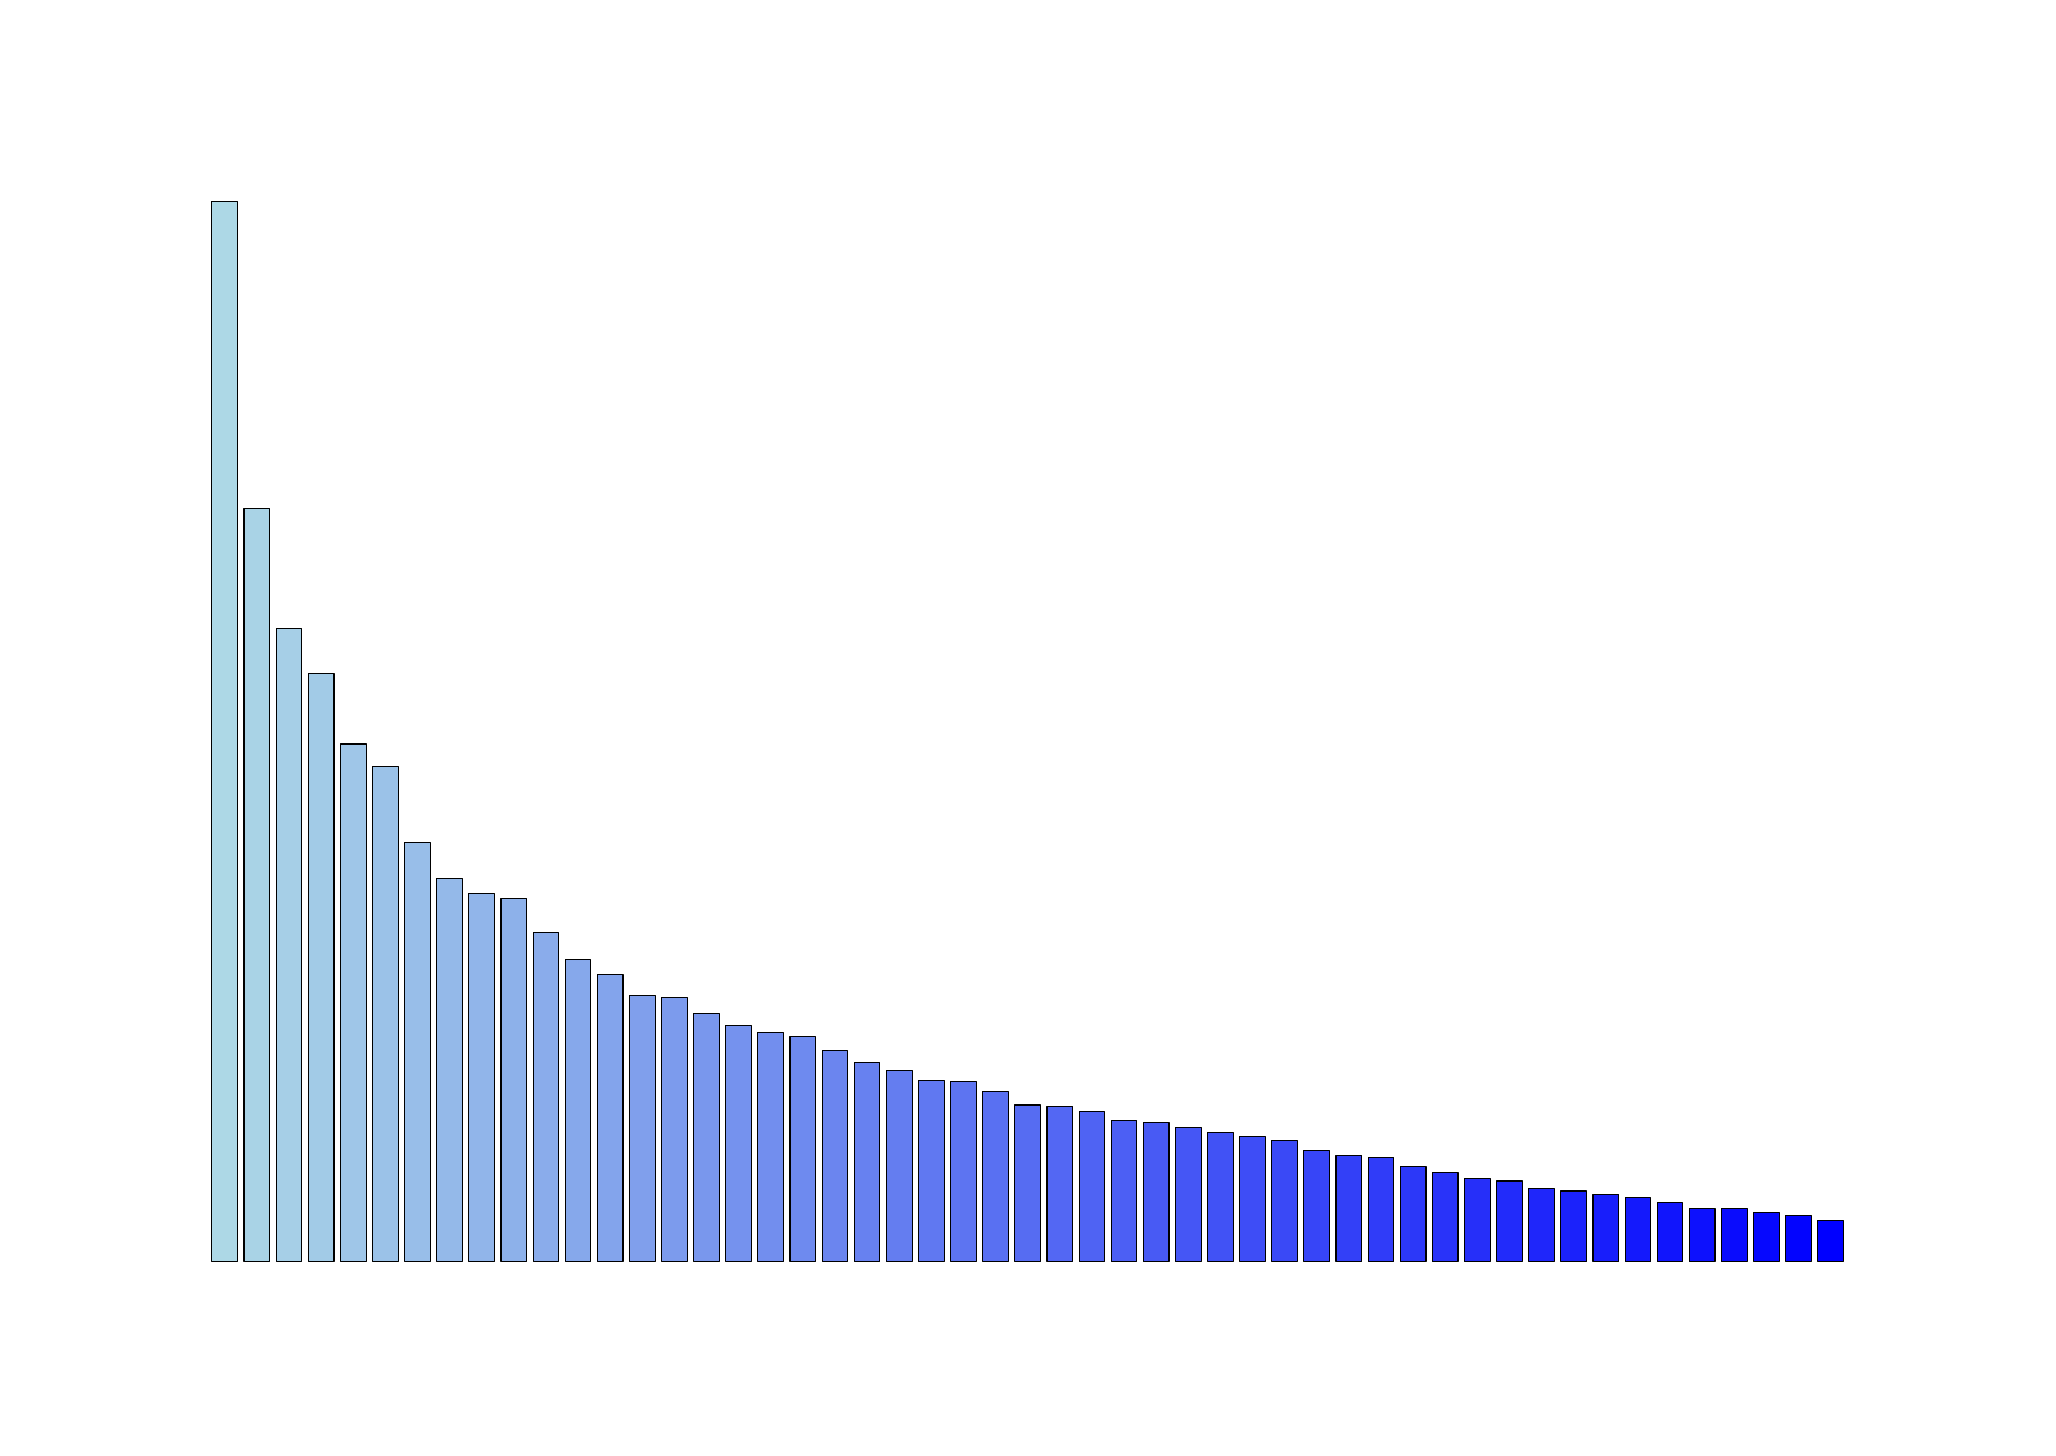
\begin{tikzpicture}[x=1pt,y=1pt]
\definecolor{fillColor}{RGB}{255,255,255}
\path[use as bounding box,fill=fillColor,fill opacity=0.00] (0,0) rectangle (722.70,505.89);
\begin{scope}
\path[clip] ( 48.00, 60.00) rectangle (674.70,457.89);
\definecolor{drawColor}{RGB}{0,0,0}
\definecolor{fillColor}{RGB}{173,216,230}

\path[draw=drawColor,line width= 0.4pt,line join=round,line cap=round,fill=fillColor] ( 66.57, 60.00) rectangle ( 75.85,443.15);
\definecolor{fillColor}{RGB}{169,211,230}

\path[draw=drawColor,line width= 0.4pt,line join=round,line cap=round,fill=fillColor] ( 78.17, 60.00) rectangle ( 87.46,332.24);
\definecolor{fillColor}{RGB}{166,207,231}

\path[draw=drawColor,line width= 0.4pt,line join=round,line cap=round,fill=fillColor] ( 89.78, 60.00) rectangle ( 99.06,288.79);
\definecolor{fillColor}{RGB}{162,203,231}

\path[draw=drawColor,line width= 0.4pt,line join=round,line cap=round,fill=fillColor] (101.39, 60.00) rectangle (110.67,272.54);
\definecolor{fillColor}{RGB}{159,198,232}

\path[draw=drawColor,line width= 0.4pt,line join=round,line cap=round,fill=fillColor] (112.99, 60.00) rectangle (122.28,247.03);
\definecolor{fillColor}{RGB}{155,194,232}

\path[draw=drawColor,line width= 0.4pt,line join=round,line cap=round,fill=fillColor] (124.60, 60.00) rectangle (133.88,238.81);
\definecolor{fillColor}{RGB}{152,190,233}

\path[draw=drawColor,line width= 0.4pt,line join=round,line cap=round,fill=fillColor] (136.20, 60.00) rectangle (145.49,211.37);
\definecolor{fillColor}{RGB}{148,185,233}

\path[draw=drawColor,line width= 0.4pt,line join=round,line cap=round,fill=fillColor] (147.81, 60.00) rectangle (157.09,198.45);
\definecolor{fillColor}{RGB}{145,181,234}

\path[draw=drawColor,line width= 0.4pt,line join=round,line cap=round,fill=fillColor] (159.41, 60.00) rectangle (168.70,193.02);
\definecolor{fillColor}{RGB}{141,177,234}

\path[draw=drawColor,line width= 0.4pt,line join=round,line cap=round,fill=fillColor] (171.02, 60.00) rectangle (180.30,191.25);
\definecolor{fillColor}{RGB}{138,172,235}

\path[draw=drawColor,line width= 0.4pt,line join=round,line cap=round,fill=fillColor] (182.62, 60.00) rectangle (191.91,178.94);
\definecolor{fillColor}{RGB}{134,168,235}

\path[draw=drawColor,line width= 0.4pt,line join=round,line cap=round,fill=fillColor] (194.23, 60.00) rectangle (203.51,169.17);
\definecolor{fillColor}{RGB}{131,164,236}

\path[draw=drawColor,line width= 0.4pt,line join=round,line cap=round,fill=fillColor] (205.84, 60.00) rectangle (215.12,163.89);
\definecolor{fillColor}{RGB}{128,159,236}

\path[draw=drawColor,line width= 0.4pt,line join=round,line cap=round,fill=fillColor] (217.44, 60.00) rectangle (226.73,156.23);
\definecolor{fillColor}{RGB}{124,155,237}

\path[draw=drawColor,line width= 0.4pt,line join=round,line cap=round,fill=fillColor] (229.05, 60.00) rectangle (238.33,155.46);
\definecolor{fillColor}{RGB}{121,151,237}

\path[draw=drawColor,line width= 0.4pt,line join=round,line cap=round,fill=fillColor] (240.65, 60.00) rectangle (249.94,149.78);
\definecolor{fillColor}{RGB}{117,146,238}

\path[draw=drawColor,line width= 0.4pt,line join=round,line cap=round,fill=fillColor] (252.26, 60.00) rectangle (261.54,145.31);
\definecolor{fillColor}{RGB}{114,142,238}

\path[draw=drawColor,line width= 0.4pt,line join=round,line cap=round,fill=fillColor] (263.86, 60.00) rectangle (273.15,142.73);
\definecolor{fillColor}{RGB}{110,138,239}

\path[draw=drawColor,line width= 0.4pt,line join=round,line cap=round,fill=fillColor] (275.47, 60.00) rectangle (284.75,141.21);
\definecolor{fillColor}{RGB}{107,133,239}

\path[draw=drawColor,line width= 0.4pt,line join=round,line cap=round,fill=fillColor] (287.07, 60.00) rectangle (296.36,136.13);
\definecolor{fillColor}{RGB}{103,129,240}

\path[draw=drawColor,line width= 0.4pt,line join=round,line cap=round,fill=fillColor] (298.68, 60.00) rectangle (307.96,131.97);
\definecolor{fillColor}{RGB}{100,125,240}

\path[draw=drawColor,line width= 0.4pt,line join=round,line cap=round,fill=fillColor] (310.29, 60.00) rectangle (319.57,129.05);
\definecolor{fillColor}{RGB}{96,120,241}

\path[draw=drawColor,line width= 0.4pt,line join=round,line cap=round,fill=fillColor] (321.89, 60.00) rectangle (331.18,125.44);
\definecolor{fillColor}{RGB}{93,116,241}

\path[draw=drawColor,line width= 0.4pt,line join=round,line cap=round,fill=fillColor] (333.50, 60.00) rectangle (342.78,124.96);
\definecolor{fillColor}{RGB}{89,112,242}

\path[draw=drawColor,line width= 0.4pt,line join=round,line cap=round,fill=fillColor] (345.10, 60.00) rectangle (354.39,121.50);
\definecolor{fillColor}{RGB}{86,108,242}

\path[draw=drawColor,line width= 0.4pt,line join=round,line cap=round,fill=fillColor] (356.71, 60.00) rectangle (365.99,116.58);
\definecolor{fillColor}{RGB}{83,103,243}

\path[draw=drawColor,line width= 0.4pt,line join=round,line cap=round,fill=fillColor] (368.31, 60.00) rectangle (377.60,116.08);
\definecolor{fillColor}{RGB}{79,99,243}

\path[draw=drawColor,line width= 0.4pt,line join=round,line cap=round,fill=fillColor] (379.92, 60.00) rectangle (389.20,114.19);
\definecolor{fillColor}{RGB}{76,95,244}

\path[draw=drawColor,line width= 0.4pt,line join=round,line cap=round,fill=fillColor] (391.52, 60.00) rectangle (400.81,111.09);
\definecolor{fillColor}{RGB}{72,90,244}

\path[draw=drawColor,line width= 0.4pt,line join=round,line cap=round,fill=fillColor] (403.13, 60.00) rectangle (412.41,110.12);
\definecolor{fillColor}{RGB}{69,86,245}

\path[draw=drawColor,line width= 0.4pt,line join=round,line cap=round,fill=fillColor] (414.74, 60.00) rectangle (424.02,108.52);
\definecolor{fillColor}{RGB}{65,82,245}

\path[draw=drawColor,line width= 0.4pt,line join=round,line cap=round,fill=fillColor] (426.34, 60.00) rectangle (435.63,106.62);
\definecolor{fillColor}{RGB}{62,77,246}

\path[draw=drawColor,line width= 0.4pt,line join=round,line cap=round,fill=fillColor] (437.95, 60.00) rectangle (447.23,105.06);
\definecolor{fillColor}{RGB}{58,73,246}

\path[draw=drawColor,line width= 0.4pt,line join=round,line cap=round,fill=fillColor] (449.55, 60.00) rectangle (458.84,103.69);
\definecolor{fillColor}{RGB}{55,69,247}

\path[draw=drawColor,line width= 0.4pt,line join=round,line cap=round,fill=fillColor] (461.16, 60.00) rectangle (470.44,100.12);
\definecolor{fillColor}{RGB}{51,64,247}

\path[draw=drawColor,line width= 0.4pt,line join=round,line cap=round,fill=fillColor] (472.76, 60.00) rectangle (482.05, 98.35);
\definecolor{fillColor}{RGB}{48,60,248}

\path[draw=drawColor,line width= 0.4pt,line join=round,line cap=round,fill=fillColor] (484.37, 60.00) rectangle (493.65, 97.66);
\definecolor{fillColor}{RGB}{44,56,248}

\path[draw=drawColor,line width= 0.4pt,line join=round,line cap=round,fill=fillColor] (495.97, 60.00) rectangle (505.26, 94.33);
\definecolor{fillColor}{RGB}{41,51,249}

\path[draw=drawColor,line width= 0.4pt,line join=round,line cap=round,fill=fillColor] (507.58, 60.00) rectangle (516.86, 92.15);
\definecolor{fillColor}{RGB}{38,47,249}

\path[draw=drawColor,line width= 0.4pt,line join=round,line cap=round,fill=fillColor] (519.19, 60.00) rectangle (528.47, 89.97);
\definecolor{fillColor}{RGB}{34,43,250}

\path[draw=drawColor,line width= 0.4pt,line join=round,line cap=round,fill=fillColor] (530.79, 60.00) rectangle (540.08, 89.15);
\definecolor{fillColor}{RGB}{31,38,250}

\path[draw=drawColor,line width= 0.4pt,line join=round,line cap=round,fill=fillColor] (542.40, 60.00) rectangle (551.68, 86.48);
\definecolor{fillColor}{RGB}{27,34,251}

\path[draw=drawColor,line width= 0.4pt,line join=round,line cap=round,fill=fillColor] (554.00, 60.00) rectangle (563.29, 85.52);
\definecolor{fillColor}{RGB}{24,30,251}

\path[draw=drawColor,line width= 0.4pt,line join=round,line cap=round,fill=fillColor] (565.61, 60.00) rectangle (574.89, 84.38);
\definecolor{fillColor}{RGB}{20,25,252}

\path[draw=drawColor,line width= 0.4pt,line join=round,line cap=round,fill=fillColor] (577.21, 60.00) rectangle (586.50, 83.02);
\definecolor{fillColor}{RGB}{17,21,252}

\path[draw=drawColor,line width= 0.4pt,line join=round,line cap=round,fill=fillColor] (588.82, 60.00) rectangle (598.10, 81.31);
\definecolor{fillColor}{RGB}{13,17,253}

\path[draw=drawColor,line width= 0.4pt,line join=round,line cap=round,fill=fillColor] (600.42, 60.00) rectangle (609.71, 79.17);
\definecolor{fillColor}{RGB}{10,12,253}

\path[draw=drawColor,line width= 0.4pt,line join=round,line cap=round,fill=fillColor] (612.03, 60.00) rectangle (621.31, 79.07);
\definecolor{fillColor}{RGB}{6,8,254}

\path[draw=drawColor,line width= 0.4pt,line join=round,line cap=round,fill=fillColor] (623.64, 60.00) rectangle (632.92, 77.63);
\definecolor{fillColor}{RGB}{3,4,254}

\path[draw=drawColor,line width= 0.4pt,line join=round,line cap=round,fill=fillColor] (635.24, 60.00) rectangle (644.53, 76.56);
\definecolor{fillColor}{RGB}{0,0,255}

\path[draw=drawColor,line width= 0.4pt,line join=round,line cap=round,fill=fillColor] (646.85, 60.00) rectangle (656.13, 74.74);
\end{scope}
\end{tikzpicture}
}
%\caption{\textit{Explained variance (blue) and cumulative explained variance (red) for $n = 51$ principal components in HFmrEF data set.}}
\end{figure}


\chapter{Source Code}
\label{chap:souce_code}

\noindent The following appendix presents all the relevant \texttt{R}-code used in this thesis. We have organized the chapter in accordance with the various steps in the machine learning procedure adopted in this thesis, see figure (\ref{fig:ML_proc_thesis}). We have tried to comment as much of the source code in order to ensure that an eventual re-examination of the results can be as easy and smooth as possible. Inquires about the code can be forwarded to the author on request.

\section{Helper Functions, \texttt{\_helper\_func.R}}
\label{sec:helper_func}

\lstinputlisting[language=R]{../../data/data_sets/source/_helper_func.R}

\section{Load Data and Labeling, \texttt{r\_data\_sets.R}}
\label{sec:load_data}

\lstinputlisting[language=R]{../../data/data_sets/raw_data/r_data_sets.R}

\section{Data Description, \texttt{desc\_data.R}}
\label{sec:app_desc_stat}

\lstinputlisting[language=R]{../../data/data_sets/source/desc_data.R}

\section{Imputation, \texttt{imputation.R}}
\label{sec:app_impu}

\lstinputlisting[language=R]{../../data/data_sets/source/imputation.R}

\section{Dimensional Reduction, \texttt{dim\_reduc.R}}
\label{sec:dim_red}


\end{document}